% Options for packages loaded elsewhere
\PassOptionsToPackage{unicode}{hyperref}
\PassOptionsToPackage{hyphens}{url}
\documentclass[
]{book}
\usepackage{xcolor}
\usepackage{amsmath,amssymb}
\setcounter{secnumdepth}{5}
\usepackage{iftex}
\ifPDFTeX
  \usepackage[T1]{fontenc}
  \usepackage[utf8]{inputenc}
  \usepackage{textcomp} % provide euro and other symbols
\else % if luatex or xetex
  \usepackage{unicode-math} % this also loads fontspec
  \defaultfontfeatures{Scale=MatchLowercase}
  \defaultfontfeatures[\rmfamily]{Ligatures=TeX,Scale=1}
\fi
\usepackage{lmodern}
\ifPDFTeX\else
  % xetex/luatex font selection
\fi
% Use upquote if available, for straight quotes in verbatim environments
\IfFileExists{upquote.sty}{\usepackage{upquote}}{}
\IfFileExists{microtype.sty}{% use microtype if available
  \usepackage[]{microtype}
  \UseMicrotypeSet[protrusion]{basicmath} % disable protrusion for tt fonts
}{}
\makeatletter
\@ifundefined{KOMAClassName}{% if non-KOMA class
  \IfFileExists{parskip.sty}{%
    \usepackage{parskip}
  }{% else
    \setlength{\parindent}{0pt}
    \setlength{\parskip}{6pt plus 2pt minus 1pt}}
}{% if KOMA class
  \KOMAoptions{parskip=half}}
\makeatother
\usepackage{color}
\usepackage{fancyvrb}
\newcommand{\VerbBar}{|}
\newcommand{\VERB}{\Verb[commandchars=\\\{\}]}
\DefineVerbatimEnvironment{Highlighting}{Verbatim}{commandchars=\\\{\}}
% Add ',fontsize=\small' for more characters per line
\usepackage{framed}
\definecolor{shadecolor}{RGB}{248,248,248}
\newenvironment{Shaded}{\begin{snugshade}}{\end{snugshade}}
\newcommand{\AlertTok}[1]{\textcolor[rgb]{0.94,0.16,0.16}{#1}}
\newcommand{\AnnotationTok}[1]{\textcolor[rgb]{0.56,0.35,0.01}{\textbf{\textit{#1}}}}
\newcommand{\AttributeTok}[1]{\textcolor[rgb]{0.13,0.29,0.53}{#1}}
\newcommand{\BaseNTok}[1]{\textcolor[rgb]{0.00,0.00,0.81}{#1}}
\newcommand{\BuiltInTok}[1]{#1}
\newcommand{\CharTok}[1]{\textcolor[rgb]{0.31,0.60,0.02}{#1}}
\newcommand{\CommentTok}[1]{\textcolor[rgb]{0.56,0.35,0.01}{\textit{#1}}}
\newcommand{\CommentVarTok}[1]{\textcolor[rgb]{0.56,0.35,0.01}{\textbf{\textit{#1}}}}
\newcommand{\ConstantTok}[1]{\textcolor[rgb]{0.56,0.35,0.01}{#1}}
\newcommand{\ControlFlowTok}[1]{\textcolor[rgb]{0.13,0.29,0.53}{\textbf{#1}}}
\newcommand{\DataTypeTok}[1]{\textcolor[rgb]{0.13,0.29,0.53}{#1}}
\newcommand{\DecValTok}[1]{\textcolor[rgb]{0.00,0.00,0.81}{#1}}
\newcommand{\DocumentationTok}[1]{\textcolor[rgb]{0.56,0.35,0.01}{\textbf{\textit{#1}}}}
\newcommand{\ErrorTok}[1]{\textcolor[rgb]{0.64,0.00,0.00}{\textbf{#1}}}
\newcommand{\ExtensionTok}[1]{#1}
\newcommand{\FloatTok}[1]{\textcolor[rgb]{0.00,0.00,0.81}{#1}}
\newcommand{\FunctionTok}[1]{\textcolor[rgb]{0.13,0.29,0.53}{\textbf{#1}}}
\newcommand{\ImportTok}[1]{#1}
\newcommand{\InformationTok}[1]{\textcolor[rgb]{0.56,0.35,0.01}{\textbf{\textit{#1}}}}
\newcommand{\KeywordTok}[1]{\textcolor[rgb]{0.13,0.29,0.53}{\textbf{#1}}}
\newcommand{\NormalTok}[1]{#1}
\newcommand{\OperatorTok}[1]{\textcolor[rgb]{0.81,0.36,0.00}{\textbf{#1}}}
\newcommand{\OtherTok}[1]{\textcolor[rgb]{0.56,0.35,0.01}{#1}}
\newcommand{\PreprocessorTok}[1]{\textcolor[rgb]{0.56,0.35,0.01}{\textit{#1}}}
\newcommand{\RegionMarkerTok}[1]{#1}
\newcommand{\SpecialCharTok}[1]{\textcolor[rgb]{0.81,0.36,0.00}{\textbf{#1}}}
\newcommand{\SpecialStringTok}[1]{\textcolor[rgb]{0.31,0.60,0.02}{#1}}
\newcommand{\StringTok}[1]{\textcolor[rgb]{0.31,0.60,0.02}{#1}}
\newcommand{\VariableTok}[1]{\textcolor[rgb]{0.00,0.00,0.00}{#1}}
\newcommand{\VerbatimStringTok}[1]{\textcolor[rgb]{0.31,0.60,0.02}{#1}}
\newcommand{\WarningTok}[1]{\textcolor[rgb]{0.56,0.35,0.01}{\textbf{\textit{#1}}}}
\usepackage{longtable,booktabs,array}
\newcounter{none} % for unnumbered tables
\usepackage{calc} % for calculating minipage widths
% Correct order of tables after \paragraph or \subparagraph
\usepackage{etoolbox}
\makeatletter
\patchcmd\longtable{\par}{\if@noskipsec\mbox{}\fi\par}{}{}
\makeatother
% Allow footnotes in longtable head/foot
\IfFileExists{footnotehyper.sty}{\usepackage{footnotehyper}}{\usepackage{footnote}}
\makesavenoteenv{longtable}
\usepackage{graphicx}
\makeatletter
\newsavebox\pandoc@box
\newcommand*\pandocbounded[1]{% scales image to fit in text height/width
  \sbox\pandoc@box{#1}%
  \Gscale@div\@tempa{\textheight}{\dimexpr\ht\pandoc@box+\dp\pandoc@box\relax}%
  \Gscale@div\@tempb{\linewidth}{\wd\pandoc@box}%
  \ifdim\@tempb\p@<\@tempa\p@\let\@tempa\@tempb\fi% select the smaller of both
  \ifdim\@tempa\p@<\p@\scalebox{\@tempa}{\usebox\pandoc@box}%
  \else\usebox{\pandoc@box}%
  \fi%
}
% Set default figure placement to htbp
\def\fps@figure{htbp}
\makeatother
\setlength{\emergencystretch}{3em} % prevent overfull lines
\providecommand{\tightlist}{%
  \setlength{\itemsep}{0pt}\setlength{\parskip}{0pt}}
\usepackage[spanish]{babel}
\usepackage{multicol}
\usepackage{titlesec}
\renewcommand{\chaptername}{Capítulo}
\usepackage{fancyhdr} \pagestyle{fancy} \fancyhf{} \fancyfoot[C]{\thepage} \fancyfoot[L]{\ifodd\value{page}\textit{\small Notas de Métodos Numéricos }\else\textit{\small Liliana Contreras-Segundo}\fi} \fancyfoot[R]{\ifodd\value{page}\textit{\small Liliana Contreras-Segundo}\else\textit{\small Notas de Métodos Numéricos}\fi}
\usepackage[left=2cm,right=2cm,top=3cm,bottom=3cm]{geometry}
\renewcommand{\chaptermark}[1]{\markboth{#1}{}}
\renewcommand{\sectionmark}[1]{\markright{#1}}
\fancyhead[LE,RO]{\nouppercase{\rightmark}}
\fancyhead[LO,RE]{\nouppercase{\leftmark}}
\usepackage{bookmark}
\IfFileExists{xurl.sty}{\usepackage{xurl}}{} % add URL line breaks if available
\urlstyle{same}
\hypersetup{
  pdftitle={Notas del curso de Métodos Numéricos},
  pdfauthor={Liliana Contreras Segundo},
  hidelinks,
  pdfcreator={LaTeX via pandoc}}

\title{Notas del curso de Métodos Numéricos}
\author{Liliana Contreras Segundo}
\date{03 December, 2025}

\begin{document}
\frontmatter
\maketitle

{
\setcounter{tocdepth}{1}
\tableofcontents
}
\mainmatter
\chapter{\texorpdfstring{\textbf{Sitemas de punto
flotante}}{Sitemas de punto flotante}}\label{sitemas-de-punto-flotante}

\section{\texorpdfstring{\emph{Ejercicio 7.1. Números de base 10 a base
2}}{Ejercicio 7.1. Números de base 10 a base 2}}\label{ejercicio-7.1.-nuxfameros-de-base-10-a-base-2}

\subsection{Ejercicio 1: 324}\label{ejercicio-1-324}

\begin{Shaded}
\begin{Highlighting}[]
\NormalTok{numero }\OtherTok{\textless{}{-}} \DecValTok{324}
\FunctionTok{cat}\NormalTok{(}\StringTok{"Convirtiendo"}\NormalTok{, numero, }\StringTok{"de base 10 a base 2:}\SpecialCharTok{\textbackslash{}n}\StringTok{"}\NormalTok{)}
\end{Highlighting}
\end{Shaded}

\begin{verbatim}
## Convirtiendo 324 de base 10 a base 2:
\end{verbatim}

\begin{Shaded}
\begin{Highlighting}[]
\NormalTok{resultado }\OtherTok{\textless{}{-}} \FunctionTok{c}\NormalTok{()}

\ControlFlowTok{while}\NormalTok{ (numero }\SpecialCharTok{\textgreater{}} \DecValTok{0}\NormalTok{) \{}
\NormalTok{  residuo }\OtherTok{\textless{}{-}}\NormalTok{ numero }\SpecialCharTok{\%\%} \DecValTok{2}
\NormalTok{  cociente }\OtherTok{\textless{}{-}}\NormalTok{ numero }\SpecialCharTok{\%/\%} \DecValTok{2}
  \FunctionTok{cat}\NormalTok{(numero, }\StringTok{"÷ 2 ="}\NormalTok{, cociente, }\StringTok{"residuo"}\NormalTok{, residuo, }\StringTok{"}\SpecialCharTok{\textbackslash{}n}\StringTok{"}\NormalTok{)}
\NormalTok{  resultado }\OtherTok{\textless{}{-}} \FunctionTok{c}\NormalTok{(residuo, resultado)}
\NormalTok{  numero }\OtherTok{\textless{}{-}}\NormalTok{ cociente}
\NormalTok{\}}
\end{Highlighting}
\end{Shaded}

\begin{verbatim}
## 324 ÷ 2 = 162 residuo 0 
## 162 ÷ 2 = 81 residuo 0 
## 81 ÷ 2 = 40 residuo 1 
## 40 ÷ 2 = 20 residuo 0 
## 20 ÷ 2 = 10 residuo 0 
## 10 ÷ 2 = 5 residuo 0 
## 5 ÷ 2 = 2 residuo 1 
## 2 ÷ 2 = 1 residuo 0 
## 1 ÷ 2 = 0 residuo 1
\end{verbatim}

\subsubsection{Resultado}\label{resultado}

\begin{Shaded}
\begin{Highlighting}[]
\NormalTok{num\_original }\OtherTok{\textless{}{-}} \DecValTok{324}

\NormalTok{binario }\OtherTok{\textless{}{-}} \FunctionTok{paste}\NormalTok{(resultado, }\AttributeTok{collapse =} \StringTok{""}\NormalTok{)}
\FunctionTok{cat}\NormalTok{(}\StringTok{"}\SpecialCharTok{\textbackslash{}n}\StringTok{Resultado:"}\NormalTok{, num\_original, }\StringTok{"en base 10 ="}\NormalTok{, binario, }\StringTok{"en base 2}\SpecialCharTok{\textbackslash{}n}\StringTok{"}\NormalTok{)}
\end{Highlighting}
\end{Shaded}

\begin{verbatim}
## 
## Resultado: 324 en base 10 = 101000100 en base 2
\end{verbatim}

\subsection{Ejercicio 2: 27}\label{ejercicio-2-27}

\begin{Shaded}
\begin{Highlighting}[]
\NormalTok{numero }\OtherTok{\textless{}{-}} \DecValTok{27}
\FunctionTok{cat}\NormalTok{(}\StringTok{"Convirtiendo"}\NormalTok{, numero, }\StringTok{"de base 10 a base 2:}\SpecialCharTok{\textbackslash{}n}\StringTok{"}\NormalTok{)}
\end{Highlighting}
\end{Shaded}

\begin{verbatim}
## Convirtiendo 27 de base 10 a base 2:
\end{verbatim}

\begin{Shaded}
\begin{Highlighting}[]
\NormalTok{resultado }\OtherTok{\textless{}{-}} \FunctionTok{c}\NormalTok{()}

\ControlFlowTok{while}\NormalTok{ (numero }\SpecialCharTok{\textgreater{}} \DecValTok{0}\NormalTok{) \{}
\NormalTok{  residuo }\OtherTok{\textless{}{-}}\NormalTok{ numero }\SpecialCharTok{\%\%} \DecValTok{2}
\NormalTok{  cociente }\OtherTok{\textless{}{-}}\NormalTok{ numero }\SpecialCharTok{\%/\%} \DecValTok{2}
  \FunctionTok{cat}\NormalTok{(numero, }\StringTok{"÷ 2 ="}\NormalTok{, cociente, }\StringTok{"residuo"}\NormalTok{, residuo, }\StringTok{"}\SpecialCharTok{\textbackslash{}n}\StringTok{"}\NormalTok{)}
\NormalTok{  resultado }\OtherTok{\textless{}{-}} \FunctionTok{c}\NormalTok{(residuo, resultado)}
\NormalTok{  numero }\OtherTok{\textless{}{-}}\NormalTok{ cociente}
\NormalTok{\}}
\end{Highlighting}
\end{Shaded}

\begin{verbatim}
## 27 ÷ 2 = 13 residuo 1 
## 13 ÷ 2 = 6 residuo 1 
## 6 ÷ 2 = 3 residuo 0 
## 3 ÷ 2 = 1 residuo 1 
## 1 ÷ 2 = 0 residuo 1
\end{verbatim}

\subsubsection{Resultado}\label{resultado-1}

\begin{Shaded}
\begin{Highlighting}[]
\NormalTok{num\_original }\OtherTok{\textless{}{-}} \DecValTok{27}

\NormalTok{binario }\OtherTok{\textless{}{-}} \FunctionTok{paste}\NormalTok{(resultado, }\AttributeTok{collapse =} \StringTok{""}\NormalTok{)}
\FunctionTok{cat}\NormalTok{(}\StringTok{"}\SpecialCharTok{\textbackslash{}n}\StringTok{Resultado:"}\NormalTok{, num\_original, }\StringTok{"en base 10 ="}\NormalTok{, binario, }\StringTok{"en base 2}\SpecialCharTok{\textbackslash{}n}\StringTok{"}\NormalTok{)}
\end{Highlighting}
\end{Shaded}

\begin{verbatim}
## 
## Resultado: 27 en base 10 = 11011 en base 2
\end{verbatim}

\subsection{Ejercicio 3: 1423}\label{ejercicio-3-1423}

\begin{Shaded}
\begin{Highlighting}[]
\NormalTok{numero }\OtherTok{\textless{}{-}} \DecValTok{1423}
\FunctionTok{cat}\NormalTok{(}\StringTok{"Convirtiendo"}\NormalTok{, numero, }\StringTok{"de base 10 a base 2:}\SpecialCharTok{\textbackslash{}n}\StringTok{"}\NormalTok{)}
\end{Highlighting}
\end{Shaded}

\begin{verbatim}
## Convirtiendo 1423 de base 10 a base 2:
\end{verbatim}

\begin{Shaded}
\begin{Highlighting}[]
\NormalTok{resultado }\OtherTok{\textless{}{-}} \FunctionTok{c}\NormalTok{()}

\ControlFlowTok{while}\NormalTok{ (numero }\SpecialCharTok{\textgreater{}} \DecValTok{0}\NormalTok{) \{}
\NormalTok{  residuo }\OtherTok{\textless{}{-}}\NormalTok{ numero }\SpecialCharTok{\%\%} \DecValTok{2}
\NormalTok{  cociente }\OtherTok{\textless{}{-}}\NormalTok{ numero }\SpecialCharTok{\%/\%} \DecValTok{2}
  \FunctionTok{cat}\NormalTok{(numero, }\StringTok{"÷ 2 ="}\NormalTok{, cociente, }\StringTok{"residuo"}\NormalTok{, residuo, }\StringTok{"}\SpecialCharTok{\textbackslash{}n}\StringTok{"}\NormalTok{)}
\NormalTok{  resultado }\OtherTok{\textless{}{-}} \FunctionTok{c}\NormalTok{(residuo, resultado)}
\NormalTok{  numero }\OtherTok{\textless{}{-}}\NormalTok{ cociente}
\NormalTok{\}}
\end{Highlighting}
\end{Shaded}

\begin{verbatim}
## 1423 ÷ 2 = 711 residuo 1 
## 711 ÷ 2 = 355 residuo 1 
## 355 ÷ 2 = 177 residuo 1 
## 177 ÷ 2 = 88 residuo 1 
## 88 ÷ 2 = 44 residuo 0 
## 44 ÷ 2 = 22 residuo 0 
## 22 ÷ 2 = 11 residuo 0 
## 11 ÷ 2 = 5 residuo 1 
## 5 ÷ 2 = 2 residuo 1 
## 2 ÷ 2 = 1 residuo 0 
## 1 ÷ 2 = 0 residuo 1
\end{verbatim}

\subsubsection{Resultado}\label{resultado-2}

\begin{Shaded}
\begin{Highlighting}[]
\NormalTok{num\_original }\OtherTok{\textless{}{-}} \DecValTok{1423}

\NormalTok{binario }\OtherTok{\textless{}{-}} \FunctionTok{paste}\NormalTok{(resultado, }\AttributeTok{collapse =} \StringTok{""}\NormalTok{)}
\FunctionTok{cat}\NormalTok{(}\StringTok{"}\SpecialCharTok{\textbackslash{}n}\StringTok{Resultado:"}\NormalTok{, num\_original, }\StringTok{"en base 10 ="}\NormalTok{, binario, }\StringTok{"en base 2}\SpecialCharTok{\textbackslash{}n}\StringTok{"}\NormalTok{)}
\end{Highlighting}
\end{Shaded}

\begin{verbatim}
## 
## Resultado: 1423 en base 10 = 10110001111 en base 2
\end{verbatim}

\subsection{Ejercicio 4: 235.25}\label{ejercicio-4-235.25}

\begin{Shaded}
\begin{Highlighting}[]
\NormalTok{numero }\OtherTok{\textless{}{-}} \FloatTok{235.25}
\FunctionTok{cat}\NormalTok{(}\StringTok{"Convirtiendo"}\NormalTok{, numero, }\StringTok{"de base 10 a base 2:}\SpecialCharTok{\textbackslash{}n}\StringTok{"}\NormalTok{)}
\end{Highlighting}
\end{Shaded}

\begin{verbatim}
## Convirtiendo 235.25 de base 10 a base 2:
\end{verbatim}

\begin{Shaded}
\begin{Highlighting}[]
\CommentTok{\# Parte ENTERA (igual que antes)}
\NormalTok{parte\_entera }\OtherTok{\textless{}{-}} \FunctionTok{floor}\NormalTok{(numero)}
\NormalTok{resultado\_entera }\OtherTok{\textless{}{-}} \FunctionTok{c}\NormalTok{()}
\NormalTok{temp }\OtherTok{\textless{}{-}}\NormalTok{ parte\_entera}

\FunctionTok{cat}\NormalTok{(}\StringTok{"{-}{-}{-} Parte entera {-}{-}{-}}\SpecialCharTok{\textbackslash{}n}\StringTok{"}\NormalTok{)}
\end{Highlighting}
\end{Shaded}

\begin{verbatim}
## --- Parte entera ---
\end{verbatim}

\begin{Shaded}
\begin{Highlighting}[]
\ControlFlowTok{while}\NormalTok{ (temp }\SpecialCharTok{\textgreater{}} \DecValTok{0}\NormalTok{) \{}
\NormalTok{  residuo }\OtherTok{\textless{}{-}}\NormalTok{ temp }\SpecialCharTok{\%\%} \DecValTok{2}
\NormalTok{  cociente }\OtherTok{\textless{}{-}}\NormalTok{ temp }\SpecialCharTok{\%/\%} \DecValTok{2}
  \FunctionTok{cat}\NormalTok{(temp, }\StringTok{"÷ 2 ="}\NormalTok{, cociente, }\StringTok{"residuo"}\NormalTok{, residuo, }\StringTok{"}\SpecialCharTok{\textbackslash{}n}\StringTok{"}\NormalTok{)}
\NormalTok{  resultado\_entera }\OtherTok{\textless{}{-}} \FunctionTok{c}\NormalTok{(residuo, resultado\_entera)}
\NormalTok{  temp }\OtherTok{\textless{}{-}}\NormalTok{ cociente}
\NormalTok{\}}
\end{Highlighting}
\end{Shaded}

\begin{verbatim}
## 235 ÷ 2 = 117 residuo 1 
## 117 ÷ 2 = 58 residuo 1 
## 58 ÷ 2 = 29 residuo 0 
## 29 ÷ 2 = 14 residuo 1 
## 14 ÷ 2 = 7 residuo 0 
## 7 ÷ 2 = 3 residuo 1 
## 3 ÷ 2 = 1 residuo 1 
## 1 ÷ 2 = 0 residuo 1
\end{verbatim}

\begin{Shaded}
\begin{Highlighting}[]
\NormalTok{binario\_entera }\OtherTok{\textless{}{-}} \FunctionTok{paste}\NormalTok{(resultado\_entera, }\AttributeTok{collapse =} \StringTok{""}\NormalTok{)}
\ControlFlowTok{if}\NormalTok{ (binario\_entera }\SpecialCharTok{==} \StringTok{""}\NormalTok{) binario\_entera }\OtherTok{\textless{}{-}} \StringTok{"0"}

\CommentTok{\# Parte DECIMAL (sin if/else)}
\NormalTok{parte\_decimal }\OtherTok{\textless{}{-}}\NormalTok{ numero }\SpecialCharTok{{-}}\NormalTok{ parte\_entera}
\NormalTok{resultado\_decimal }\OtherTok{\textless{}{-}} \FunctionTok{c}\NormalTok{()}
\NormalTok{temp }\OtherTok{\textless{}{-}}\NormalTok{ parte\_decimal}

\FunctionTok{cat}\NormalTok{(}\StringTok{"{-}{-}{-} Parte decimal {-}{-}{-}}\SpecialCharTok{\textbackslash{}n}\StringTok{"}\NormalTok{)}
\end{Highlighting}
\end{Shaded}

\begin{verbatim}
## --- Parte decimal ---
\end{verbatim}

\begin{Shaded}
\begin{Highlighting}[]
\NormalTok{contador }\OtherTok{\textless{}{-}} \DecValTok{0}
\ControlFlowTok{while}\NormalTok{ (temp }\SpecialCharTok{\textgreater{}} \DecValTok{0} \SpecialCharTok{\&\&}\NormalTok{ contador }\SpecialCharTok{\textless{}} \DecValTok{8}\NormalTok{) \{}
\NormalTok{  temp }\OtherTok{\textless{}{-}}\NormalTok{ temp }\SpecialCharTok{*} \DecValTok{2}
  
\NormalTok{  digito }\OtherTok{\textless{}{-}} \FunctionTok{floor}\NormalTok{(temp)  }
\NormalTok{  resultado\_decimal }\OtherTok{\textless{}{-}} \FunctionTok{c}\NormalTok{(resultado\_decimal, digito)}
  \FunctionTok{cat}\NormalTok{(temp, }\StringTok{"→ dígito"}\NormalTok{, digito, }\StringTok{"}\SpecialCharTok{\textbackslash{}n}\StringTok{"}\NormalTok{)}
\NormalTok{  temp }\OtherTok{\textless{}{-}}\NormalTok{ temp }\SpecialCharTok{{-}}\NormalTok{ digito }
\NormalTok{  contador }\OtherTok{\textless{}{-}}\NormalTok{ contador }\SpecialCharTok{+} \DecValTok{1}
\NormalTok{\}}
\end{Highlighting}
\end{Shaded}

\begin{verbatim}
## 0.5 → dígito 0 
## 1 → dígito 1
\end{verbatim}

\begin{Shaded}
\begin{Highlighting}[]
\NormalTok{binario\_decimal }\OtherTok{\textless{}{-}} \FunctionTok{paste}\NormalTok{(resultado\_decimal, }\AttributeTok{collapse =} \StringTok{""}\NormalTok{)}

\FunctionTok{cat}\NormalTok{(}\StringTok{"}\SpecialCharTok{\textbackslash{}n}\StringTok{Resultado:"}\NormalTok{, numero, }\StringTok{"="}\NormalTok{, binario\_entera, }\StringTok{"."}\NormalTok{, binario\_decimal, }\StringTok{"en base 2}\SpecialCharTok{\textbackslash{}n}\StringTok{"}\NormalTok{)}
\end{Highlighting}
\end{Shaded}

\begin{verbatim}
## 
## Resultado: 235.25 = 11101011 . 01 en base 2
\end{verbatim}

\subsection{Ejercicio 4: 41.596}\label{ejercicio-4-41.596}

\begin{Shaded}
\begin{Highlighting}[]
\NormalTok{numero }\OtherTok{\textless{}{-}} \FloatTok{41.596}
\FunctionTok{cat}\NormalTok{(}\StringTok{"Convirtiendo"}\NormalTok{, numero, }\StringTok{"de base 10 a base 2:}\SpecialCharTok{\textbackslash{}n}\StringTok{"}\NormalTok{)}
\end{Highlighting}
\end{Shaded}

\begin{verbatim}
## Convirtiendo 41.596 de base 10 a base 2:
\end{verbatim}

\begin{Shaded}
\begin{Highlighting}[]
\CommentTok{\# Parte ENTERA (igual que antes)}
\NormalTok{parte\_entera }\OtherTok{\textless{}{-}} \FunctionTok{floor}\NormalTok{(numero)}
\NormalTok{resultado\_entera }\OtherTok{\textless{}{-}} \FunctionTok{c}\NormalTok{()}
\NormalTok{temp }\OtherTok{\textless{}{-}}\NormalTok{ parte\_entera}

\FunctionTok{cat}\NormalTok{(}\StringTok{"{-}{-}{-} Parte entera {-}{-}{-}}\SpecialCharTok{\textbackslash{}n}\StringTok{"}\NormalTok{)}
\end{Highlighting}
\end{Shaded}

\begin{verbatim}
## --- Parte entera ---
\end{verbatim}

\begin{Shaded}
\begin{Highlighting}[]
\ControlFlowTok{while}\NormalTok{ (temp }\SpecialCharTok{\textgreater{}} \DecValTok{0}\NormalTok{) \{}
\NormalTok{  residuo }\OtherTok{\textless{}{-}}\NormalTok{ temp }\SpecialCharTok{\%\%} \DecValTok{2}
\NormalTok{  cociente }\OtherTok{\textless{}{-}}\NormalTok{ temp }\SpecialCharTok{\%/\%} \DecValTok{2}
  \FunctionTok{cat}\NormalTok{(temp, }\StringTok{"÷ 2 ="}\NormalTok{, cociente, }\StringTok{"residuo"}\NormalTok{, residuo, }\StringTok{"}\SpecialCharTok{\textbackslash{}n}\StringTok{"}\NormalTok{)}
\NormalTok{  resultado\_entera }\OtherTok{\textless{}{-}} \FunctionTok{c}\NormalTok{(residuo, resultado\_entera)}
\NormalTok{  temp }\OtherTok{\textless{}{-}}\NormalTok{ cociente}
\NormalTok{\}}
\end{Highlighting}
\end{Shaded}

\begin{verbatim}
## 41 ÷ 2 = 20 residuo 1 
## 20 ÷ 2 = 10 residuo 0 
## 10 ÷ 2 = 5 residuo 0 
## 5 ÷ 2 = 2 residuo 1 
## 2 ÷ 2 = 1 residuo 0 
## 1 ÷ 2 = 0 residuo 1
\end{verbatim}

\begin{Shaded}
\begin{Highlighting}[]
\NormalTok{binario\_entera }\OtherTok{\textless{}{-}} \FunctionTok{paste}\NormalTok{(resultado\_entera, }\AttributeTok{collapse =} \StringTok{""}\NormalTok{)}
\ControlFlowTok{if}\NormalTok{ (binario\_entera }\SpecialCharTok{==} \StringTok{""}\NormalTok{) binario\_entera }\OtherTok{\textless{}{-}} \StringTok{"0"}

\NormalTok{parte\_decimal }\OtherTok{\textless{}{-}}\NormalTok{ numero }\SpecialCharTok{{-}}\NormalTok{ parte\_entera}
\NormalTok{resultado\_decimal }\OtherTok{\textless{}{-}} \FunctionTok{c}\NormalTok{()}
\NormalTok{temp }\OtherTok{\textless{}{-}}\NormalTok{ parte\_decimal}

\FunctionTok{cat}\NormalTok{(}\StringTok{"{-}{-}{-} Parte decimal {-}{-}{-}}\SpecialCharTok{\textbackslash{}n}\StringTok{"}\NormalTok{)}
\end{Highlighting}
\end{Shaded}

\begin{verbatim}
## --- Parte decimal ---
\end{verbatim}

\begin{Shaded}
\begin{Highlighting}[]
\NormalTok{contador }\OtherTok{\textless{}{-}} \DecValTok{0}
\ControlFlowTok{while}\NormalTok{ (temp }\SpecialCharTok{\textgreater{}} \DecValTok{0} \SpecialCharTok{\&\&}\NormalTok{ contador }\SpecialCharTok{\textless{}} \DecValTok{8}\NormalTok{) \{}
\NormalTok{  temp }\OtherTok{\textless{}{-}}\NormalTok{ temp }\SpecialCharTok{*} \DecValTok{2}

\NormalTok{  digito }\OtherTok{\textless{}{-}} \FunctionTok{floor}\NormalTok{(temp)  }
\NormalTok{  resultado\_decimal }\OtherTok{\textless{}{-}} \FunctionTok{c}\NormalTok{(resultado\_decimal, digito)}
  \FunctionTok{cat}\NormalTok{(temp, }\StringTok{"→ dígito"}\NormalTok{, digito, }\StringTok{"}\SpecialCharTok{\textbackslash{}n}\StringTok{"}\NormalTok{)}
\NormalTok{  temp }\OtherTok{\textless{}{-}}\NormalTok{ temp }\SpecialCharTok{{-}}\NormalTok{ digito  }
\NormalTok{  contador }\OtherTok{\textless{}{-}}\NormalTok{ contador }\SpecialCharTok{+} \DecValTok{1}
\NormalTok{\}}
\end{Highlighting}
\end{Shaded}

\begin{verbatim}
## 1.192 → dígito 1 
## 0.384 → dígito 0 
## 0.768 → dígito 0 
## 1.536 → dígito 1 
## 1.072 → dígito 1 
## 0.144 → dígito 0 
## 0.288 → dígito 0 
## 0.576 → dígito 0
\end{verbatim}

\begin{Shaded}
\begin{Highlighting}[]
\NormalTok{binario\_decimal }\OtherTok{\textless{}{-}} \FunctionTok{paste}\NormalTok{(resultado\_decimal, }\AttributeTok{collapse =} \StringTok{""}\NormalTok{)}

\FunctionTok{cat}\NormalTok{(}\StringTok{"}\SpecialCharTok{\textbackslash{}n}\StringTok{Resultado:"}\NormalTok{, numero, }\StringTok{"="}\NormalTok{, binario\_entera, }\StringTok{"."}\NormalTok{, binario\_decimal, }\StringTok{"en base 2}\SpecialCharTok{\textbackslash{}n}\StringTok{"}\NormalTok{)}
\end{Highlighting}
\end{Shaded}

\begin{verbatim}
## 
## Resultado: 41.596 = 101001 . 10011000 en base 2
\end{verbatim}

\section{\texorpdfstring{\emph{Ejercicio
7.2:}}{Ejercicio 7.2:}}\label{ejercicio-7.2}

\subsection{1. Realizar una revisión de la historia de los métodos
numéricos, elaborar un documento de hasta dos
cuartillas:}\label{realizar-una-revisiuxf3n-de-la-historia-de-los-muxe9todos-numuxe9ricos-elaborar-un-documento-de-hasta-dos-cuartillas}

\subsection{Historia y Evolución de los Métodos
Numéricos}\label{historia-y-evoluciuxf3n-de-los-muxe9todos-numuxe9ricos}

Los métodos numéricos constituyen una herramienta fundamental en la
ciencia y la ingeniería moderna, permitiendo resolver problemas
complejos que la matemática analítica no puede abordar de forma
eficiente o exacta. Se definen como procesos matemáticos iterativos
diseñados para encontrar una aproximación a una solución específica con
un error previamente determinado (Cortés Rosas et al., 2019). La
historia de estos métodos es, en esencia, la crónica de la búsqueda
humana por cuantificar, predecir y comprender el mundo a través de la
aproximación sucesiva.

Los Orígenes: La Antigüedad y las Primeras Aproximaciones

La necesidad de emplear métodos numéricos es tan antigua como las
matemáticas mismas. Uno de los ejemplos más tempranos se remonta al 1650
a.C., con los Papiros de Rhyad, que contenían técnicas para resolver
expresiones matemáticas sin álgebra. Un hito fundamental ocurrió
alrededor del 250 a.C., cuando Euclides desarrolló el \textbf{Método
Exhaustivo}, utilizando figuras geométricas inscritas en un círculo para
aproximar el valor de π. Este método representaba un principio iterativo
rudimentario: al aumentar el número de lados del polígono, la
aproximación al área del círculo (y por ende a π) se hacía más precisa.

Posteriormente, en el Siglo IX d.C., el matemático persa Al-Juarismi
sentó las bases de los algoritmos, que son el corazón de cualquier
método numérico. Sin embargo, fue durante el Siglo XVII y XVIII cuando
se sentaron las bases teóricas más sólidas. Isaac Newton y Gottfried
Leibniz, con la creación del cálculo diferencial e integral, abrieron la
puerta a la resolución de problemas de cambio y movimiento. Figuras como
Brook Taylor, con su serie de polinomios para aproximar funciones, y
Leonhard Euler, con soluciones numéricas para ecuaciones diferenciales,
proporcionaron las herramientas analíticas que más tarde se convertirían
en algoritmos computacionales.

La Revolución de la Computación: La Materialización de los Métodos

Hasta el siglo XIX, la aplicación de estos métodos era una tarea
extenuante y propensa a errores, realizada manualmente por calculistas.
La invención de máquinas como la \textbf{Máquina Diferencial} de Charles
Babbage (1822) y las ideas de Ada Lovelace sobre programación marcaron
un punto de inflexión. La historia de los métodos numéricos se volvió, a
partir de entonces, paralela a la historia de la computación (Cortés
Rosas et al., 2019). El siglo XX aceleró esta simbiosis. Alan Turing,
con su concepto de una máquina universal en 1937, y John Von Neumann,
con la arquitectura de computadoras stored-program, crearon el hardware
necesario. Por otro lado, la necesidad de realizar cálculos balísticos y
de energía nuclear durante la Segunda Guerra Mundial impulsó el
desarrollo de métodos aplicados. Matemáticos como J. H. Wilkinson en el
Reino Unido trabajaron en algoritmos para resolver sistemas de
ecuaciones y calcular eigenvalores, problemas críticos para la
ingeniería. La creación de lenguajes de programación de alto nivel, como
FORTRAN por John Backus en 1953, democratizó el uso de estos métodos,
permitiendo a los científicos escribir instrucciones complejas de manera
más sencilla. Proyectos de software matemático como EISPACK y LINPACK
(décadas de 1970 y 1980) estandarizaron y optimizaron las rutinas
numéricas. La culminación de esta tendencia fue el desarrollo de
entornos como MATLAB por Cleve Moler en 1984, que integró poderosos
métodos numéricos en una interfaz accesible, revolucionando la enseñanza
y la práctica en ingeniería.

La Necesidad en la Ingeniería y el Manejo del Error

La ingeniería, como disciplina que aplica las ciencias básicas para
resolver problemas reales, rara vez se enfrenta a modelos lineales o con
soluciones exactas y enteras (Cortés Rosas et al., 2019). Los sistemas
del mundo real ---desde la aerodinámica de un avión hasta la resistencia
de un puente--- se modelan con ecuaciones no lineales y diferenciales
cuya solución analítica es imposible o impráctica de obtener. Es aquí
donde los métodos numéricos se vuelven indispensables. A diferencia de
los ejercicios algebraicos ideales, los métodos numéricos aceptan la
imposibilidad de una solución perfecta y la sustituyen por una
aproximación controlada. Mediante iteraciones, un valor inicial se
refina sucesivamente hasta cumplir con una tolerancia de error
predefinida. Sin embargo, esta potencia tiene una contrapartida
fundamental: la gestión del error. Cada aproximación conlleva
inherentemente errores de redondeo, truncamiento y modelado. Por lo
tanto, un aspecto crucial del análisis numérico moderno no es solo la
eficiencia del método, sino también el entendimiento y la cuantificación
de estos errores para garantizar que la solución sea suficientemente
buena para su aplicación práctica. En conclusión, la historia de los
métodos numéricos es un viaje desde la intuición geométrica de los
antiguos hasta el cálculo de alta precisión impulsado por las
supercomputadoras. Su evolución ha estado ligada al ingenio humano para
crear herramientas, primero conceptuales como el algoritmo y luego
físicas como la computadora, que permiten transformar problemas
irresolubles analíticamente en soluciones numéricas prácticas y
confiables, convirtiéndose en un pilar sin el cual la ingeniería moderna
no podría existir.

Referencia Cortés Rosas, J. J., González Cárdenas, M. E., Pinilla Morán,
V. D., Salazar Moreno, A., \& Tovar Pérez, V. H. (2019). Aproximación
numérica y errores. Facultad de Ingeniería, UNAM. Proyecto PAPIME
PE105717

\subsection{2. Realiza las siguientes conversiones de base 10 a base
2}\label{realiza-las-siguientes-conversiones-de-base-10-a-base-2}

\subsubsection{a) 246:}\label{a-246}

\begin{Shaded}
\begin{Highlighting}[]
\NormalTok{numero }\OtherTok{\textless{}{-}} \DecValTok{246}
\FunctionTok{cat}\NormalTok{(}\StringTok{"Convirtiendo"}\NormalTok{, numero, }\StringTok{"de base 10 a base 2:}\SpecialCharTok{\textbackslash{}n}\StringTok{"}\NormalTok{)}
\end{Highlighting}
\end{Shaded}

\begin{verbatim}
## Convirtiendo 246 de base 10 a base 2:
\end{verbatim}

\begin{Shaded}
\begin{Highlighting}[]
\NormalTok{resultado }\OtherTok{\textless{}{-}} \FunctionTok{c}\NormalTok{()}

\ControlFlowTok{while}\NormalTok{ (numero }\SpecialCharTok{\textgreater{}} \DecValTok{0}\NormalTok{) \{}
\NormalTok{  residuo }\OtherTok{\textless{}{-}}\NormalTok{ numero }\SpecialCharTok{\%\%} \DecValTok{2}
\NormalTok{  cociente }\OtherTok{\textless{}{-}}\NormalTok{ numero }\SpecialCharTok{\%/\%} \DecValTok{2}
  \FunctionTok{cat}\NormalTok{(numero, }\StringTok{"÷ 2 ="}\NormalTok{, cociente, }\StringTok{"residuo"}\NormalTok{, residuo, }\StringTok{"}\SpecialCharTok{\textbackslash{}n}\StringTok{"}\NormalTok{)}
\NormalTok{  resultado }\OtherTok{\textless{}{-}} \FunctionTok{c}\NormalTok{(residuo, resultado)}
\NormalTok{  numero }\OtherTok{\textless{}{-}}\NormalTok{ cociente}
\NormalTok{\}}
\end{Highlighting}
\end{Shaded}

\begin{verbatim}
## 246 ÷ 2 = 123 residuo 0 
## 123 ÷ 2 = 61 residuo 1 
## 61 ÷ 2 = 30 residuo 1 
## 30 ÷ 2 = 15 residuo 0 
## 15 ÷ 2 = 7 residuo 1 
## 7 ÷ 2 = 3 residuo 1 
## 3 ÷ 2 = 1 residuo 1 
## 1 ÷ 2 = 0 residuo 1
\end{verbatim}

\begin{Shaded}
\begin{Highlighting}[]
\NormalTok{num\_original }\OtherTok{\textless{}{-}} \DecValTok{246}
\CommentTok{\# Mostrar resultado}
\NormalTok{binario }\OtherTok{\textless{}{-}} \FunctionTok{paste}\NormalTok{(resultado, }\AttributeTok{collapse =} \StringTok{""}\NormalTok{)}
\FunctionTok{cat}\NormalTok{(}\StringTok{"}\SpecialCharTok{\textbackslash{}n}\StringTok{Resultado:"}\NormalTok{, num\_original, }\StringTok{"en base 10 ="}\NormalTok{, binario, }\StringTok{"en base 2}\SpecialCharTok{\textbackslash{}n}\StringTok{"}\NormalTok{)}
\end{Highlighting}
\end{Shaded}

\begin{verbatim}
## 
## Resultado: 246 en base 10 = 11110110 en base 2
\end{verbatim}

\subsubsection{b) 345.68:}\label{b-345.68}

\begin{Shaded}
\begin{Highlighting}[]
\NormalTok{numero }\OtherTok{\textless{}{-}} \FloatTok{345.68}
\FunctionTok{cat}\NormalTok{(}\StringTok{"Convirtiendo"}\NormalTok{, numero, }\StringTok{"de base 10 a base 2:}\SpecialCharTok{\textbackslash{}n}\StringTok{"}\NormalTok{)}
\end{Highlighting}
\end{Shaded}

\begin{verbatim}
## Convirtiendo 345.68 de base 10 a base 2:
\end{verbatim}

\begin{Shaded}
\begin{Highlighting}[]
\CommentTok{\# Parte ENTERA (igual que antes)}
\NormalTok{parte\_entera }\OtherTok{\textless{}{-}} \FunctionTok{floor}\NormalTok{(numero)}
\NormalTok{resultado\_entera }\OtherTok{\textless{}{-}} \FunctionTok{c}\NormalTok{()}
\NormalTok{temp }\OtherTok{\textless{}{-}}\NormalTok{ parte\_entera}

\FunctionTok{cat}\NormalTok{(}\StringTok{"{-}{-}{-} Parte entera {-}{-}{-}}\SpecialCharTok{\textbackslash{}n}\StringTok{"}\NormalTok{)}
\end{Highlighting}
\end{Shaded}

\begin{verbatim}
## --- Parte entera ---
\end{verbatim}

\begin{Shaded}
\begin{Highlighting}[]
\ControlFlowTok{while}\NormalTok{ (temp }\SpecialCharTok{\textgreater{}} \DecValTok{0}\NormalTok{) \{}
\NormalTok{  residuo }\OtherTok{\textless{}{-}}\NormalTok{ temp }\SpecialCharTok{\%\%} \DecValTok{2}
\NormalTok{  cociente }\OtherTok{\textless{}{-}}\NormalTok{ temp }\SpecialCharTok{\%/\%} \DecValTok{2}
  \FunctionTok{cat}\NormalTok{(temp, }\StringTok{"÷ 2 ="}\NormalTok{, cociente, }\StringTok{"residuo"}\NormalTok{, residuo, }\StringTok{"}\SpecialCharTok{\textbackslash{}n}\StringTok{"}\NormalTok{)}
\NormalTok{  resultado\_entera }\OtherTok{\textless{}{-}} \FunctionTok{c}\NormalTok{(residuo, resultado\_entera)}
\NormalTok{  temp }\OtherTok{\textless{}{-}}\NormalTok{ cociente}
\NormalTok{\}}
\end{Highlighting}
\end{Shaded}

\begin{verbatim}
## 345 ÷ 2 = 172 residuo 1 
## 172 ÷ 2 = 86 residuo 0 
## 86 ÷ 2 = 43 residuo 0 
## 43 ÷ 2 = 21 residuo 1 
## 21 ÷ 2 = 10 residuo 1 
## 10 ÷ 2 = 5 residuo 0 
## 5 ÷ 2 = 2 residuo 1 
## 2 ÷ 2 = 1 residuo 0 
## 1 ÷ 2 = 0 residuo 1
\end{verbatim}

\begin{Shaded}
\begin{Highlighting}[]
\NormalTok{binario\_entera }\OtherTok{\textless{}{-}} \FunctionTok{paste}\NormalTok{(resultado\_entera, }\AttributeTok{collapse =} \StringTok{""}\NormalTok{)}
\ControlFlowTok{if}\NormalTok{ (binario\_entera }\SpecialCharTok{==} \StringTok{""}\NormalTok{) binario\_entera }\OtherTok{\textless{}{-}} \StringTok{"0"}

\NormalTok{parte\_decimal }\OtherTok{\textless{}{-}}\NormalTok{ numero }\SpecialCharTok{{-}}\NormalTok{ parte\_entera}
\NormalTok{resultado\_decimal }\OtherTok{\textless{}{-}} \FunctionTok{c}\NormalTok{()}
\NormalTok{temp }\OtherTok{\textless{}{-}}\NormalTok{ parte\_decimal}

\FunctionTok{cat}\NormalTok{(}\StringTok{"{-}{-}{-} Parte decimal {-}{-}{-}}\SpecialCharTok{\textbackslash{}n}\StringTok{"}\NormalTok{)}
\end{Highlighting}
\end{Shaded}

\begin{verbatim}
## --- Parte decimal ---
\end{verbatim}

\begin{Shaded}
\begin{Highlighting}[]
\NormalTok{contador }\OtherTok{\textless{}{-}} \DecValTok{0}
\ControlFlowTok{while}\NormalTok{ (temp }\SpecialCharTok{\textgreater{}} \DecValTok{0} \SpecialCharTok{\&\&}\NormalTok{ contador }\SpecialCharTok{\textless{}} \DecValTok{8}\NormalTok{) \{}
\NormalTok{  temp }\OtherTok{\textless{}{-}}\NormalTok{ temp }\SpecialCharTok{*} \DecValTok{2}

\NormalTok{  digito }\OtherTok{\textless{}{-}} \FunctionTok{floor}\NormalTok{(temp)  }
\NormalTok{  resultado\_decimal }\OtherTok{\textless{}{-}} \FunctionTok{c}\NormalTok{(resultado\_decimal, digito)}
  \FunctionTok{cat}\NormalTok{(temp, }\StringTok{"→ dígito"}\NormalTok{, digito, }\StringTok{"}\SpecialCharTok{\textbackslash{}n}\StringTok{"}\NormalTok{)}
\NormalTok{  temp }\OtherTok{\textless{}{-}}\NormalTok{ temp }\SpecialCharTok{{-}}\NormalTok{ digito  }
\NormalTok{  contador }\OtherTok{\textless{}{-}}\NormalTok{ contador }\SpecialCharTok{+} \DecValTok{1}
\NormalTok{\}}
\end{Highlighting}
\end{Shaded}

\begin{verbatim}
## 1.36 → dígito 1 
## 0.72 → dígito 0 
## 1.44 → dígito 1 
## 0.88 → dígito 0 
## 1.76 → dígito 1 
## 1.52 → dígito 1 
## 1.04 → dígito 1 
## 0.08 → dígito 0
\end{verbatim}

\begin{Shaded}
\begin{Highlighting}[]
\NormalTok{binario\_decimal }\OtherTok{\textless{}{-}} \FunctionTok{paste}\NormalTok{(resultado\_decimal, }\AttributeTok{collapse =} \StringTok{""}\NormalTok{)}

\FunctionTok{cat}\NormalTok{(}\StringTok{"}\SpecialCharTok{\textbackslash{}n}\StringTok{Resultado:"}\NormalTok{, numero, }\StringTok{"="}\NormalTok{, binario\_entera, }\StringTok{"."}\NormalTok{, binario\_decimal, }\StringTok{"en base 2}\SpecialCharTok{\textbackslash{}n}\StringTok{"}\NormalTok{)}
\end{Highlighting}
\end{Shaded}

\begin{verbatim}
## 
## Resultado: 345.68 = 101011001 . 10101110 en base 2
\end{verbatim}

\subsubsection{c) 4586632.2846:}\label{c-4586632.2846}

\begin{Shaded}
\begin{Highlighting}[]
\NormalTok{numero }\OtherTok{\textless{}{-}} \FloatTok{4586632.2846}
\FunctionTok{cat}\NormalTok{(}\StringTok{"Convirtiendo"}\NormalTok{, numero, }\StringTok{"de base 10 a base 2:}\SpecialCharTok{\textbackslash{}n}\StringTok{"}\NormalTok{)}
\end{Highlighting}
\end{Shaded}

\begin{verbatim}
## Convirtiendo 4586632 de base 10 a base 2:
\end{verbatim}

\begin{Shaded}
\begin{Highlighting}[]
\CommentTok{\# Parte ENTERA (igual que antes)}
\NormalTok{parte\_entera }\OtherTok{\textless{}{-}} \FunctionTok{floor}\NormalTok{(numero)}
\NormalTok{resultado\_entera }\OtherTok{\textless{}{-}} \FunctionTok{c}\NormalTok{()}
\NormalTok{temp }\OtherTok{\textless{}{-}}\NormalTok{ parte\_entera}

\FunctionTok{cat}\NormalTok{(}\StringTok{"{-}{-}{-} Parte entera {-}{-}{-}}\SpecialCharTok{\textbackslash{}n}\StringTok{"}\NormalTok{)}
\end{Highlighting}
\end{Shaded}

\begin{verbatim}
## --- Parte entera ---
\end{verbatim}

\begin{Shaded}
\begin{Highlighting}[]
\ControlFlowTok{while}\NormalTok{ (temp }\SpecialCharTok{\textgreater{}} \DecValTok{0}\NormalTok{) \{}
\NormalTok{  residuo }\OtherTok{\textless{}{-}}\NormalTok{ temp }\SpecialCharTok{\%\%} \DecValTok{2}
\NormalTok{  cociente }\OtherTok{\textless{}{-}}\NormalTok{ temp }\SpecialCharTok{\%/\%} \DecValTok{2}
  \FunctionTok{cat}\NormalTok{(temp, }\StringTok{"÷ 2 ="}\NormalTok{, cociente, }\StringTok{"residuo"}\NormalTok{, residuo, }\StringTok{"}\SpecialCharTok{\textbackslash{}n}\StringTok{"}\NormalTok{)}
\NormalTok{  resultado\_entera }\OtherTok{\textless{}{-}} \FunctionTok{c}\NormalTok{(residuo, resultado\_entera)}
\NormalTok{  temp }\OtherTok{\textless{}{-}}\NormalTok{ cociente}
\NormalTok{\}}
\end{Highlighting}
\end{Shaded}

\begin{verbatim}
## 4586632 ÷ 2 = 2293316 residuo 0 
## 2293316 ÷ 2 = 1146658 residuo 0 
## 1146658 ÷ 2 = 573329 residuo 0 
## 573329 ÷ 2 = 286664 residuo 1 
## 286664 ÷ 2 = 143332 residuo 0 
## 143332 ÷ 2 = 71666 residuo 0 
## 71666 ÷ 2 = 35833 residuo 0 
## 35833 ÷ 2 = 17916 residuo 1 
## 17916 ÷ 2 = 8958 residuo 0 
## 8958 ÷ 2 = 4479 residuo 0 
## 4479 ÷ 2 = 2239 residuo 1 
## 2239 ÷ 2 = 1119 residuo 1 
## 1119 ÷ 2 = 559 residuo 1 
## 559 ÷ 2 = 279 residuo 1 
## 279 ÷ 2 = 139 residuo 1 
## 139 ÷ 2 = 69 residuo 1 
## 69 ÷ 2 = 34 residuo 1 
## 34 ÷ 2 = 17 residuo 0 
## 17 ÷ 2 = 8 residuo 1 
## 8 ÷ 2 = 4 residuo 0 
## 4 ÷ 2 = 2 residuo 0 
## 2 ÷ 2 = 1 residuo 0 
## 1 ÷ 2 = 0 residuo 1
\end{verbatim}

\begin{Shaded}
\begin{Highlighting}[]
\NormalTok{binario\_entera }\OtherTok{\textless{}{-}} \FunctionTok{paste}\NormalTok{(resultado\_entera, }\AttributeTok{collapse =} \StringTok{""}\NormalTok{)}
\ControlFlowTok{if}\NormalTok{ (binario\_entera }\SpecialCharTok{==} \StringTok{""}\NormalTok{) binario\_entera }\OtherTok{\textless{}{-}} \StringTok{"0"}

\NormalTok{parte\_decimal }\OtherTok{\textless{}{-}}\NormalTok{ numero }\SpecialCharTok{{-}}\NormalTok{ parte\_entera}
\NormalTok{resultado\_decimal }\OtherTok{\textless{}{-}} \FunctionTok{c}\NormalTok{()}
\NormalTok{temp }\OtherTok{\textless{}{-}}\NormalTok{ parte\_decimal}

\FunctionTok{cat}\NormalTok{(}\StringTok{"{-}{-}{-} Parte decimal {-}{-}{-}}\SpecialCharTok{\textbackslash{}n}\StringTok{"}\NormalTok{)}
\end{Highlighting}
\end{Shaded}

\begin{verbatim}
## --- Parte decimal ---
\end{verbatim}

\begin{Shaded}
\begin{Highlighting}[]
\NormalTok{contador }\OtherTok{\textless{}{-}} \DecValTok{0}
\ControlFlowTok{while}\NormalTok{ (temp }\SpecialCharTok{\textgreater{}} \DecValTok{0} \SpecialCharTok{\&\&}\NormalTok{ contador }\SpecialCharTok{\textless{}} \DecValTok{8}\NormalTok{) \{}
\NormalTok{  temp }\OtherTok{\textless{}{-}}\NormalTok{ temp }\SpecialCharTok{*} \DecValTok{2}

\NormalTok{  digito }\OtherTok{\textless{}{-}} \FunctionTok{floor}\NormalTok{(temp)  }
\NormalTok{  resultado\_decimal }\OtherTok{\textless{}{-}} \FunctionTok{c}\NormalTok{(resultado\_decimal, digito)}
  \FunctionTok{cat}\NormalTok{(temp, }\StringTok{"→ dígito"}\NormalTok{, digito, }\StringTok{"}\SpecialCharTok{\textbackslash{}n}\StringTok{"}\NormalTok{)}
\NormalTok{  temp }\OtherTok{\textless{}{-}}\NormalTok{ temp }\SpecialCharTok{{-}}\NormalTok{ digito  }
\NormalTok{  contador }\OtherTok{\textless{}{-}}\NormalTok{ contador }\SpecialCharTok{+} \DecValTok{1}
\NormalTok{\}}
\end{Highlighting}
\end{Shaded}

\begin{verbatim}
## 0.5692 → dígito 0 
## 1.1384 → dígito 1 
## 0.2768 → dígito 0 
## 0.5536 → dígito 0 
## 1.1072 → dígito 1 
## 0.2144 → dígito 0 
## 0.4288 → dígito 0 
## 0.8576 → dígito 0
\end{verbatim}

\begin{Shaded}
\begin{Highlighting}[]
\NormalTok{binario\_decimal }\OtherTok{\textless{}{-}} \FunctionTok{paste}\NormalTok{(resultado\_decimal, }\AttributeTok{collapse =} \StringTok{""}\NormalTok{)}

\FunctionTok{cat}\NormalTok{(}\StringTok{"}\SpecialCharTok{\textbackslash{}n}\StringTok{Resultado:"}\NormalTok{, numero, }\StringTok{"="}\NormalTok{, binario\_entera, }\StringTok{"."}\NormalTok{, binario\_decimal, }\StringTok{"en base 2}\SpecialCharTok{\textbackslash{}n}\StringTok{"}\NormalTok{)}
\end{Highlighting}
\end{Shaded}

\begin{verbatim}
## 
## Resultado: 4586632 = 10001011111110010001000 . 01001000 en base 2
\end{verbatim}

\subsubsection{d) 984365.27463:}\label{d-984365.27463}

\begin{Shaded}
\begin{Highlighting}[]
\NormalTok{numero }\OtherTok{\textless{}{-}} \FloatTok{984365.27463}
\FunctionTok{cat}\NormalTok{(}\StringTok{"Convirtiendo"}\NormalTok{, numero, }\StringTok{"de base 10 a base 2:}\SpecialCharTok{\textbackslash{}n}\StringTok{"}\NormalTok{)}
\end{Highlighting}
\end{Shaded}

\begin{verbatim}
## Convirtiendo 984365.3 de base 10 a base 2:
\end{verbatim}

\begin{Shaded}
\begin{Highlighting}[]
\CommentTok{\# Parte ENTERA (igual que antes)}
\NormalTok{parte\_entera }\OtherTok{\textless{}{-}} \FunctionTok{floor}\NormalTok{(numero)}
\NormalTok{resultado\_entera }\OtherTok{\textless{}{-}} \FunctionTok{c}\NormalTok{()}
\NormalTok{temp }\OtherTok{\textless{}{-}}\NormalTok{ parte\_entera}

\FunctionTok{cat}\NormalTok{(}\StringTok{"{-}{-}{-} Parte entera {-}{-}{-}}\SpecialCharTok{\textbackslash{}n}\StringTok{"}\NormalTok{)}
\end{Highlighting}
\end{Shaded}

\begin{verbatim}
## --- Parte entera ---
\end{verbatim}

\begin{Shaded}
\begin{Highlighting}[]
\ControlFlowTok{while}\NormalTok{ (temp }\SpecialCharTok{\textgreater{}} \DecValTok{0}\NormalTok{) \{}
\NormalTok{  residuo }\OtherTok{\textless{}{-}}\NormalTok{ temp }\SpecialCharTok{\%\%} \DecValTok{2}
\NormalTok{  cociente }\OtherTok{\textless{}{-}}\NormalTok{ temp }\SpecialCharTok{\%/\%} \DecValTok{2}
  \FunctionTok{cat}\NormalTok{(temp, }\StringTok{"÷ 2 ="}\NormalTok{, cociente, }\StringTok{"residuo"}\NormalTok{, residuo, }\StringTok{"}\SpecialCharTok{\textbackslash{}n}\StringTok{"}\NormalTok{)}
\NormalTok{  resultado\_entera }\OtherTok{\textless{}{-}} \FunctionTok{c}\NormalTok{(residuo, resultado\_entera)}
\NormalTok{  temp }\OtherTok{\textless{}{-}}\NormalTok{ cociente}
\NormalTok{\}}
\end{Highlighting}
\end{Shaded}

\begin{verbatim}
## 984365 ÷ 2 = 492182 residuo 1 
## 492182 ÷ 2 = 246091 residuo 0 
## 246091 ÷ 2 = 123045 residuo 1 
## 123045 ÷ 2 = 61522 residuo 1 
## 61522 ÷ 2 = 30761 residuo 0 
## 30761 ÷ 2 = 15380 residuo 1 
## 15380 ÷ 2 = 7690 residuo 0 
## 7690 ÷ 2 = 3845 residuo 0 
## 3845 ÷ 2 = 1922 residuo 1 
## 1922 ÷ 2 = 961 residuo 0 
## 961 ÷ 2 = 480 residuo 1 
## 480 ÷ 2 = 240 residuo 0 
## 240 ÷ 2 = 120 residuo 0 
## 120 ÷ 2 = 60 residuo 0 
## 60 ÷ 2 = 30 residuo 0 
## 30 ÷ 2 = 15 residuo 0 
## 15 ÷ 2 = 7 residuo 1 
## 7 ÷ 2 = 3 residuo 1 
## 3 ÷ 2 = 1 residuo 1 
## 1 ÷ 2 = 0 residuo 1
\end{verbatim}

\begin{Shaded}
\begin{Highlighting}[]
\NormalTok{binario\_entera }\OtherTok{\textless{}{-}} \FunctionTok{paste}\NormalTok{(resultado\_entera, }\AttributeTok{collapse =} \StringTok{""}\NormalTok{)}
\ControlFlowTok{if}\NormalTok{ (binario\_entera }\SpecialCharTok{==} \StringTok{""}\NormalTok{) binario\_entera }\OtherTok{\textless{}{-}} \StringTok{"0"}

\NormalTok{parte\_decimal }\OtherTok{\textless{}{-}}\NormalTok{ numero }\SpecialCharTok{{-}}\NormalTok{ parte\_entera}
\NormalTok{resultado\_decimal }\OtherTok{\textless{}{-}} \FunctionTok{c}\NormalTok{()}
\NormalTok{temp }\OtherTok{\textless{}{-}}\NormalTok{ parte\_decimal}

\FunctionTok{cat}\NormalTok{(}\StringTok{"{-}{-}{-} Parte decimal {-}{-}{-}}\SpecialCharTok{\textbackslash{}n}\StringTok{"}\NormalTok{)}
\end{Highlighting}
\end{Shaded}

\begin{verbatim}
## --- Parte decimal ---
\end{verbatim}

\begin{Shaded}
\begin{Highlighting}[]
\NormalTok{contador }\OtherTok{\textless{}{-}} \DecValTok{0}
\ControlFlowTok{while}\NormalTok{ (temp }\SpecialCharTok{\textgreater{}} \DecValTok{0} \SpecialCharTok{\&\&}\NormalTok{ contador }\SpecialCharTok{\textless{}} \DecValTok{8}\NormalTok{) \{}
\NormalTok{  temp }\OtherTok{\textless{}{-}}\NormalTok{ temp }\SpecialCharTok{*} \DecValTok{2}

\NormalTok{  digito }\OtherTok{\textless{}{-}} \FunctionTok{floor}\NormalTok{(temp)  }
\NormalTok{  resultado\_decimal }\OtherTok{\textless{}{-}} \FunctionTok{c}\NormalTok{(resultado\_decimal, digito)}
  \FunctionTok{cat}\NormalTok{(temp, }\StringTok{"→ dígito"}\NormalTok{, digito, }\StringTok{"}\SpecialCharTok{\textbackslash{}n}\StringTok{"}\NormalTok{)}
\NormalTok{  temp }\OtherTok{\textless{}{-}}\NormalTok{ temp }\SpecialCharTok{{-}}\NormalTok{ digito  }
\NormalTok{  contador }\OtherTok{\textless{}{-}}\NormalTok{ contador }\SpecialCharTok{+} \DecValTok{1}
\NormalTok{\}}
\end{Highlighting}
\end{Shaded}

\begin{verbatim}
## 0.54926 → dígito 0 
## 1.09852 → dígito 1 
## 0.19704 → dígito 0 
## 0.39408 → dígito 0 
## 0.78816 → dígito 0 
## 1.57632 → dígito 1 
## 1.15264 → dígito 1 
## 0.30528 → dígito 0
\end{verbatim}

\begin{Shaded}
\begin{Highlighting}[]
\NormalTok{binario\_decimal }\OtherTok{\textless{}{-}} \FunctionTok{paste}\NormalTok{(resultado\_decimal, }\AttributeTok{collapse =} \StringTok{""}\NormalTok{)}

\FunctionTok{cat}\NormalTok{(}\StringTok{"}\SpecialCharTok{\textbackslash{}n}\StringTok{Resultado:"}\NormalTok{, numero, }\StringTok{"="}\NormalTok{, binario\_entera, }\StringTok{"."}\NormalTok{, binario\_decimal, }\StringTok{"en base 2}\SpecialCharTok{\textbackslash{}n}\StringTok{"}\NormalTok{)}
\end{Highlighting}
\end{Shaded}

\begin{verbatim}
## 
## Resultado: 984365.3 = 11110000010100101101 . 01000110 en base 2
\end{verbatim}

\subsubsection{e) 79905523:}\label{e-79905523}

\begin{Shaded}
\begin{Highlighting}[]
\NormalTok{numero }\OtherTok{\textless{}{-}} \DecValTok{79905523}
\FunctionTok{cat}\NormalTok{(}\StringTok{"Convirtiendo"}\NormalTok{, numero, }\StringTok{"de base 10 a base 2:}\SpecialCharTok{\textbackslash{}n}\StringTok{"}\NormalTok{)}
\end{Highlighting}
\end{Shaded}

\begin{verbatim}
## Convirtiendo 79905523 de base 10 a base 2:
\end{verbatim}

\begin{Shaded}
\begin{Highlighting}[]
\NormalTok{resultado }\OtherTok{\textless{}{-}} \FunctionTok{c}\NormalTok{()}

\ControlFlowTok{while}\NormalTok{ (numero }\SpecialCharTok{\textgreater{}} \DecValTok{0}\NormalTok{) \{}
\NormalTok{  residuo }\OtherTok{\textless{}{-}}\NormalTok{ numero }\SpecialCharTok{\%\%} \DecValTok{2}
\NormalTok{  cociente }\OtherTok{\textless{}{-}}\NormalTok{ numero }\SpecialCharTok{\%/\%} \DecValTok{2}
  \FunctionTok{cat}\NormalTok{(numero, }\StringTok{"÷ 2 ="}\NormalTok{, cociente, }\StringTok{"residuo"}\NormalTok{, residuo, }\StringTok{"}\SpecialCharTok{\textbackslash{}n}\StringTok{"}\NormalTok{)}
\NormalTok{  resultado }\OtherTok{\textless{}{-}} \FunctionTok{c}\NormalTok{(residuo, resultado)}
\NormalTok{  numero }\OtherTok{\textless{}{-}}\NormalTok{ cociente}
\NormalTok{\}}
\end{Highlighting}
\end{Shaded}

\begin{verbatim}
## 79905523 ÷ 2 = 39952761 residuo 1 
## 39952761 ÷ 2 = 19976380 residuo 1 
## 19976380 ÷ 2 = 9988190 residuo 0 
## 9988190 ÷ 2 = 4994095 residuo 0 
## 4994095 ÷ 2 = 2497047 residuo 1 
## 2497047 ÷ 2 = 1248523 residuo 1 
## 1248523 ÷ 2 = 624261 residuo 1 
## 624261 ÷ 2 = 312130 residuo 1 
## 312130 ÷ 2 = 156065 residuo 0 
## 156065 ÷ 2 = 78032 residuo 1 
## 78032 ÷ 2 = 39016 residuo 0 
## 39016 ÷ 2 = 19508 residuo 0 
## 19508 ÷ 2 = 9754 residuo 0 
## 9754 ÷ 2 = 4877 residuo 0 
## 4877 ÷ 2 = 2438 residuo 1 
## 2438 ÷ 2 = 1219 residuo 0 
## 1219 ÷ 2 = 609 residuo 1 
## 609 ÷ 2 = 304 residuo 1 
## 304 ÷ 2 = 152 residuo 0 
## 152 ÷ 2 = 76 residuo 0 
## 76 ÷ 2 = 38 residuo 0 
## 38 ÷ 2 = 19 residuo 0 
## 19 ÷ 2 = 9 residuo 1 
## 9 ÷ 2 = 4 residuo 1 
## 4 ÷ 2 = 2 residuo 0 
## 2 ÷ 2 = 1 residuo 0 
## 1 ÷ 2 = 0 residuo 1
\end{verbatim}

\begin{Shaded}
\begin{Highlighting}[]
\NormalTok{num\_original }\OtherTok{\textless{}{-}} \DecValTok{79905523}
\CommentTok{\# Mostrar resultado}
\NormalTok{binario }\OtherTok{\textless{}{-}} \FunctionTok{paste}\NormalTok{(resultado, }\AttributeTok{collapse =} \StringTok{""}\NormalTok{)}
\FunctionTok{cat}\NormalTok{(}\StringTok{"}\SpecialCharTok{\textbackslash{}n}\StringTok{Resultado:"}\NormalTok{, num\_original, }\StringTok{"en base 10 ="}\NormalTok{, binario, }\StringTok{"en base 2}\SpecialCharTok{\textbackslash{}n}\StringTok{"}\NormalTok{)}
\end{Highlighting}
\end{Shaded}

\begin{verbatim}
## 
## Resultado: 79905523 en base 10 = 100110000110100001011110011 en base 2
\end{verbatim}

\subsection{4. Describe exhaustivamente los tipos de errores que
existen:}\label{describe-exhaustivamente-los-tipos-de-errores-que-existen}

\chapter{Descripción Exhaustiva de los Tipos de Errores en el Análisis
Numérico}\label{descripciuxf3n-exhaustiva-de-los-tipos-de-errores-en-el-anuxe1lisis-numuxe9rico}

En el ámbito de la ingeniería y las ciencias, trabajar con modelos
matemáticos es una práctica común. Sin embargo, estos modelos son
abstracciones que rara vez capturan la totalidad de un fenómeno físico,
y los instrumentos de cálculo tienen limitaciones inherentes. La
diferencia entre un valor considerado real y el valor obtenido a través
de mediciones o cálculos se conoce como error. Comprender, clasificar y
cuantificar estos errores es fundamental para validar cualquier
resultado numérico.

\section{Exactitud y Precisión: Conceptos
Fundamentales}\label{exactitud-y-precisiuxf3n-conceptos-fundamentales}

Antes de profundizar en los errores, es crucial distinguir entre dos
conceptos often confundidos: exactitud y precisión. Exactitud: Se
refiere a la cercanía de una medición o cálculo al valor verdadero o
aceptado como real. Un método numérico es exacto si, en promedio, sus
resultados se acercan mucho al valor real.

Precisión: Se refiere a la dispersión o reproducibilidad de las
mediciones o cálculos. Un método es preciso si, al repetirse en las
mismas condiciones, produce resultados muy similares entre sí, incluso
si todos están lejos del valor real. En el contexto de los métodos
numéricos, se busca que las iteraciones sucesivas sean precisas
(converjan a un valor estable) y que este valor sea exacto (se aproxime
lo máximo posible a la solución verdadera).

\section{Clasificación de los
Errores}\label{clasificaciuxf3n-de-los-errores}

Los errores se pueden clasificar en dos grandes grupos según su origen:
los errores inherentes y los errores del método.

\begin{enumerate}
\def\labelenumi{\arabic{enumi}.}
\tightlist
\item
  Errores Inherentes o del Modelo
\end{enumerate}

Estos errores son intrínsecos al problema mismo y existen antes de que
se realice cualquier cálculo. Son producto de las simplificaciones
necesarias para crear un modelo matemático manejable y de las
limitaciones físicas de la medición. Estos errores no se pueden eliminar
por completo, solo minimizar, y son muy difíciles de cuantificar con
precisión. Dentro de esta categoría se encuentran:

Incertidumbres: Surgen de la imposibilidad de medir dimensiones físicas
de forma exacta debido a la naturaleza de la materia y a las
imperfecciones de los instrumentos de medición. Por ejemplo, medir la
longitud de una barra con un calibrador siempre tendrá un margen de
incertidumbre.

Verdaderas Equivocaciones: Son errores humanos inadvertidos en la
lectura de instrumentos, el traslado de información o la configuración
de un experimento. Un ejemplo clásico es la ceguera de taller, donde un
operario lee mal un instrumento por familiaridad.

\begin{enumerate}
\def\labelenumi{\arabic{enumi}.}
\setcounter{enumi}{1}
\tightlist
\item
  Errores del Método
\end{enumerate}

Estos errores se introducen durante el proceso de cálculo y son
consecuencia de las limitaciones en la representación y manipulación de
cantidades numéricas en dispositivos como calculadoras y computadoras. A
diferencia de los inherentes, los errores del método sí pueden
cuantificarse y controlarse. Los dos tipos principales son:

Error por Truncamiento: Ocurre cuando un proceso matemático infinito se
corta o trunca para ser manejado de forma finita. El ejemplo más claro
es el uso de series de Taylor para aproximar una función. Si solo usamos
los primeros 5 términos de una serie infinita, estamos truncando el
resto, y la diferencia entre la suma infinita y la suma de 5 términos es
el error por truncamiento.

Error por Redondeo: Se produce porque los computadores tienen una
capacidad limitada para representar cifras (usando aritmética de punto
flotante). Cuando un número tiene más dígitos de los que la máquina
puede almacenar, debe ser redondeado. Las reglas comunes de redondeo
son:

Si el dígito siguiente al último significativo es mayor que 5, se
incrementa en uno el último dígito significativo.

Si es menor que 5, el último dígito significativo permanece igual.

Si es exactamente 5, se suele redondear al número par más cercano
(redondeo simétrico) para minimizar el sesgo estadístico.

Es importante destacar que, según estudios clásicos como el de McCracken
y Dorn (1984), la magnitud del error por truncamiento es generalmente
mayor que la del error por redondeo simétrico.

\section{Cuantificación de los
Errores}\label{cuantificaciuxf3n-de-los-errores}

Para evaluar la calidad de una aproximación, es esencial medir el error.
Se utilizan dos medidas principales:

\begin{enumerate}
\def\labelenumi{\arabic{enumi}.}
\item
  Error Absoluto (E) Es la diferencia absoluta entre un valor de
  referencia (que se considera \textbf{real}) y el valor aproximado. E =
  \textbar{} V\_real - V\_aproximado \textbar{} El error absoluto tiene
  las mismas unidades que la magnitud medida, lo que a veces dificulta
  la interpretación de su significado.
\item
  Error Relativo (e) Expresa el error absoluto en relación con el tamaño
  del valor real, típicamente como un porcentaje. Al ser adimensional,
  permite comparar la precisión de mediciones de magnitudes diferentes.
  e = ( \textbar{} V\_real - V\_aproximado \textbar{} / V\_real ) *
  100\%
\end{enumerate}

Consideración Práctica sobre el \textbf{Valor Real}

En la práctica, el verdadero valor real (V\_real) casi nunca se conoce.
Por lo tanto, en el contexto de los métodos numéricos iterativos, se usa
una aproximación pragmática:

Se toma el valor de la iteración más reciente (V\_i) como la mejor
aproximación disponible. Se calcula el error comparándolo con el valor
de la iteración anterior (V\_\{i-1\}). Así, las fórmulas prácticas se
convierten en:

Error Absoluto (entre iteraciones): E = \textbar{} V\_i - V\_\{i-1\}
\textbar{}

Error Relativo (entre iteraciones): e = ( \textbar{} V\_i - V\_\{i-1\}
\textbar{} / V\_i ) * 100\%

El proceso iterativo se detiene cuando el error absoluto o relativo cae
por debajo de una tolerancia predefinida, asegurando que la solución es
suficientemente buena para los fines deseados.

\section{Referencia}\label{referencia}

Cortés Rosas, J. J., González Cárdenas, M. E., Pinilla Morán, V. D.,
Salazar Moreno, A., \& Tovar Pérez, V. H. (2019). Aproximación numérica
y errores. Facultad de Ingeniería, UNAM. Proyecto PAPIME PE105717.

\chapter{\texorpdfstring{\textbf{Sistemas de ecuaciones
lineales}}{Sistemas de ecuaciones lineales}}\label{sistemas-de-ecuaciones-lineales}

\section{Ejercicios a mano}\label{ejercicios-a-mano}

\begin{figure}
\centering
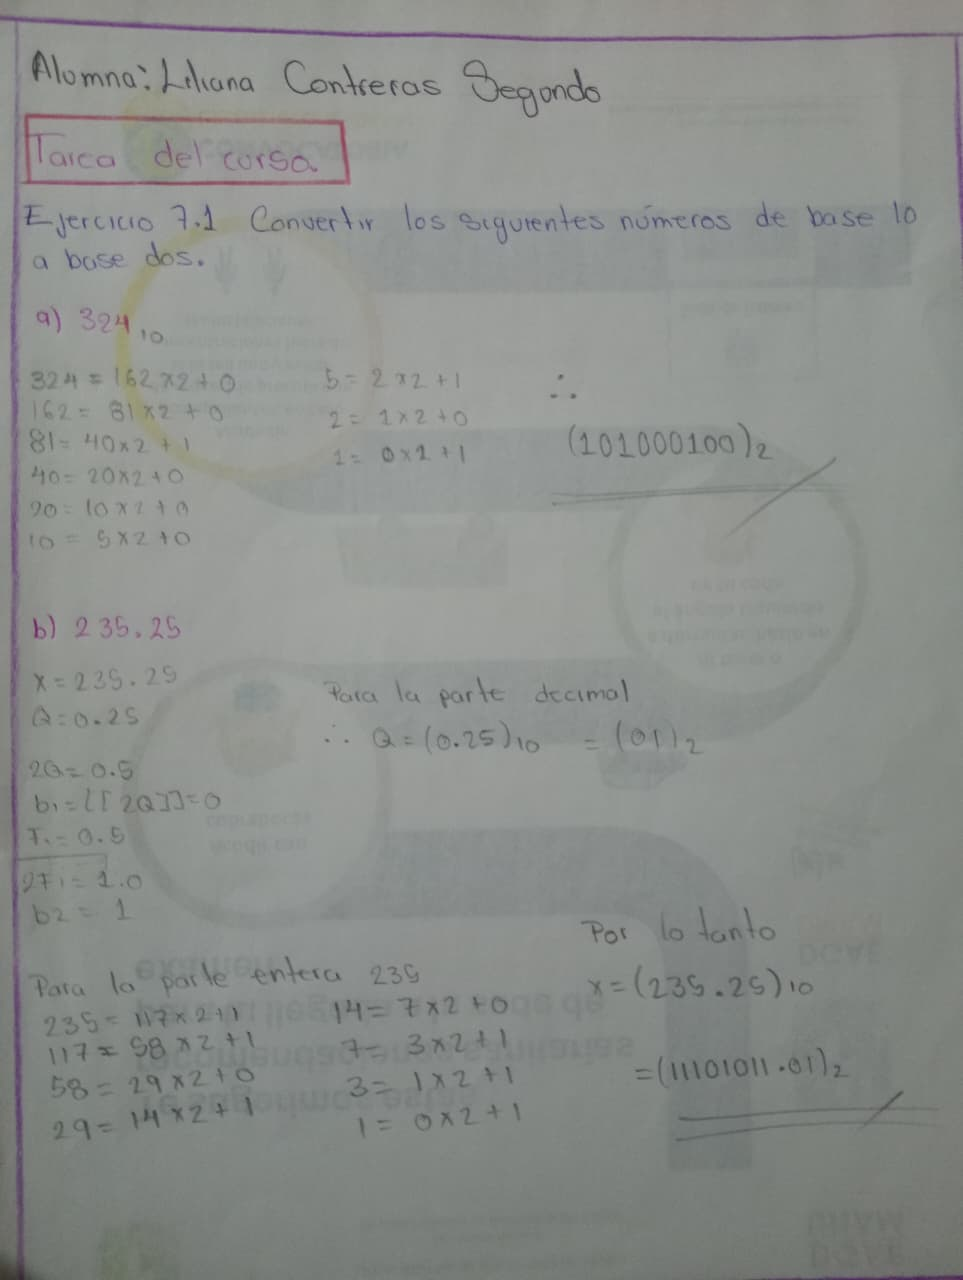
\includegraphics[width=2.60417in,height=\textheight,keepaspectratio,alt={pag.1}]{1.jpg}
\caption{pag.1}
\end{figure}

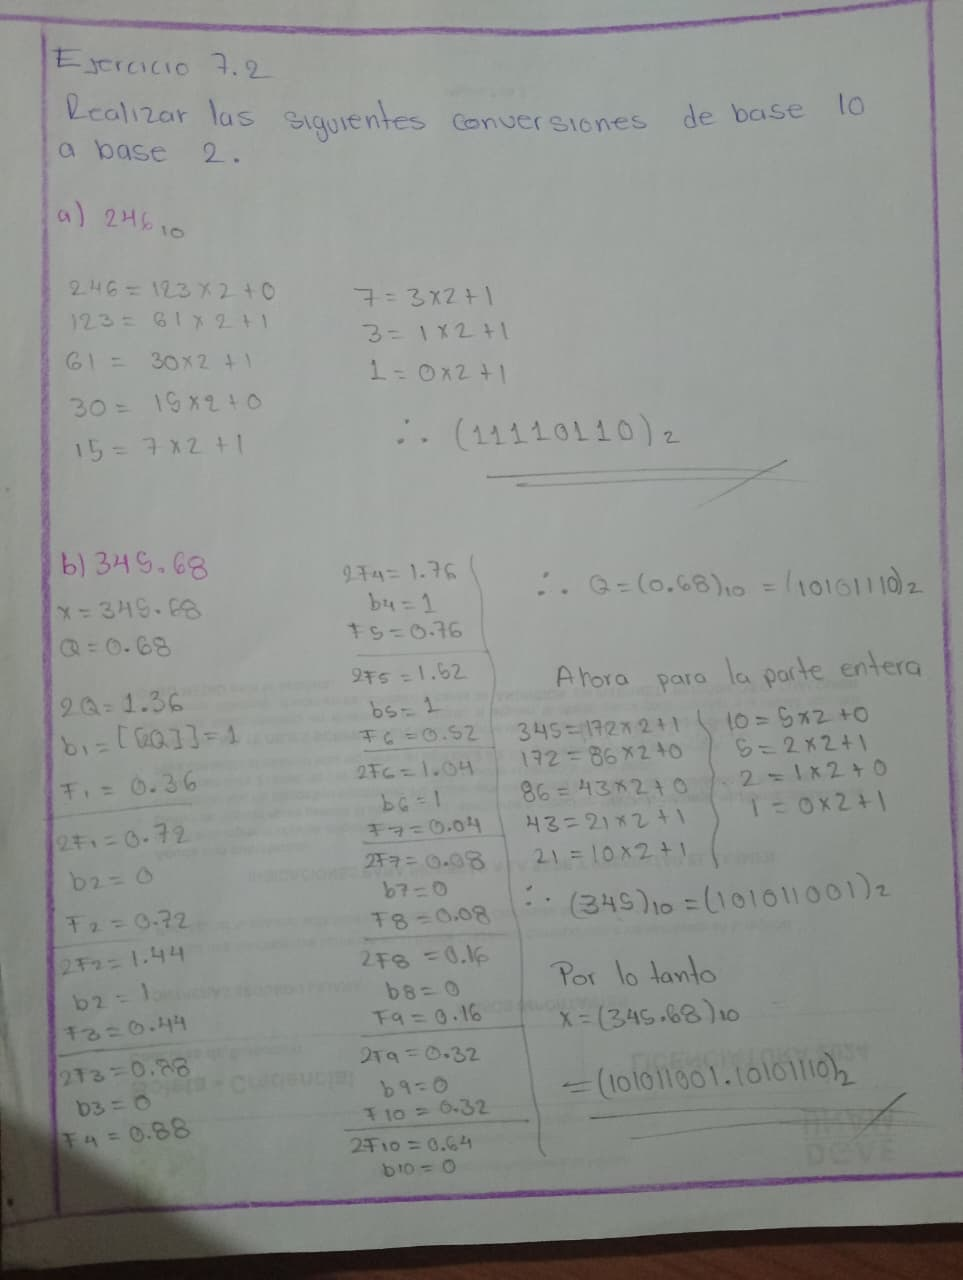
\includegraphics[width=2.60417in,height=\textheight,keepaspectratio,alt={pag.2}]{2.jpg}
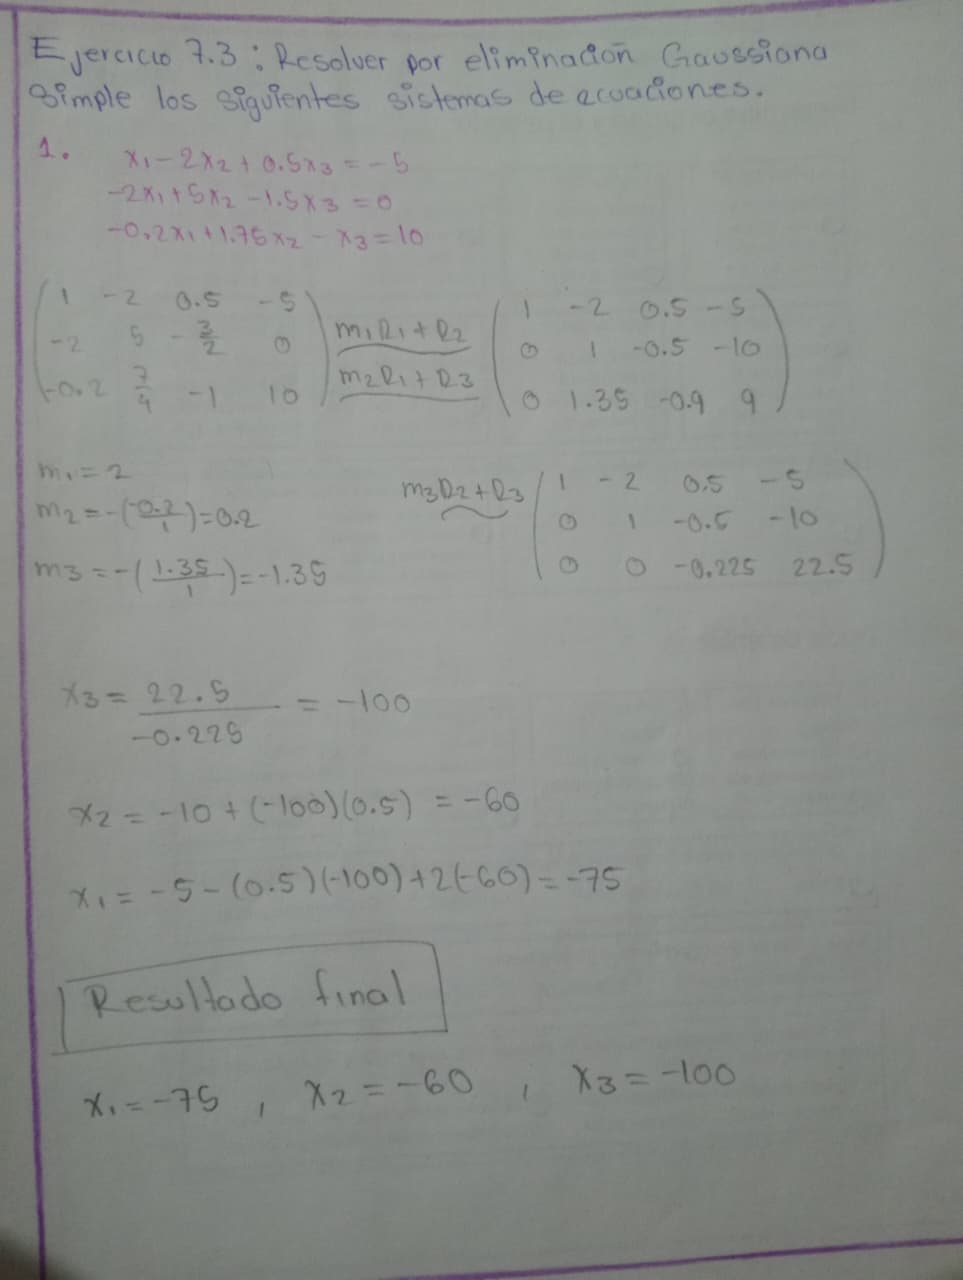
\includegraphics[width=2.60417in,height=\textheight,keepaspectratio,alt={pag.3}]{3.jpg}
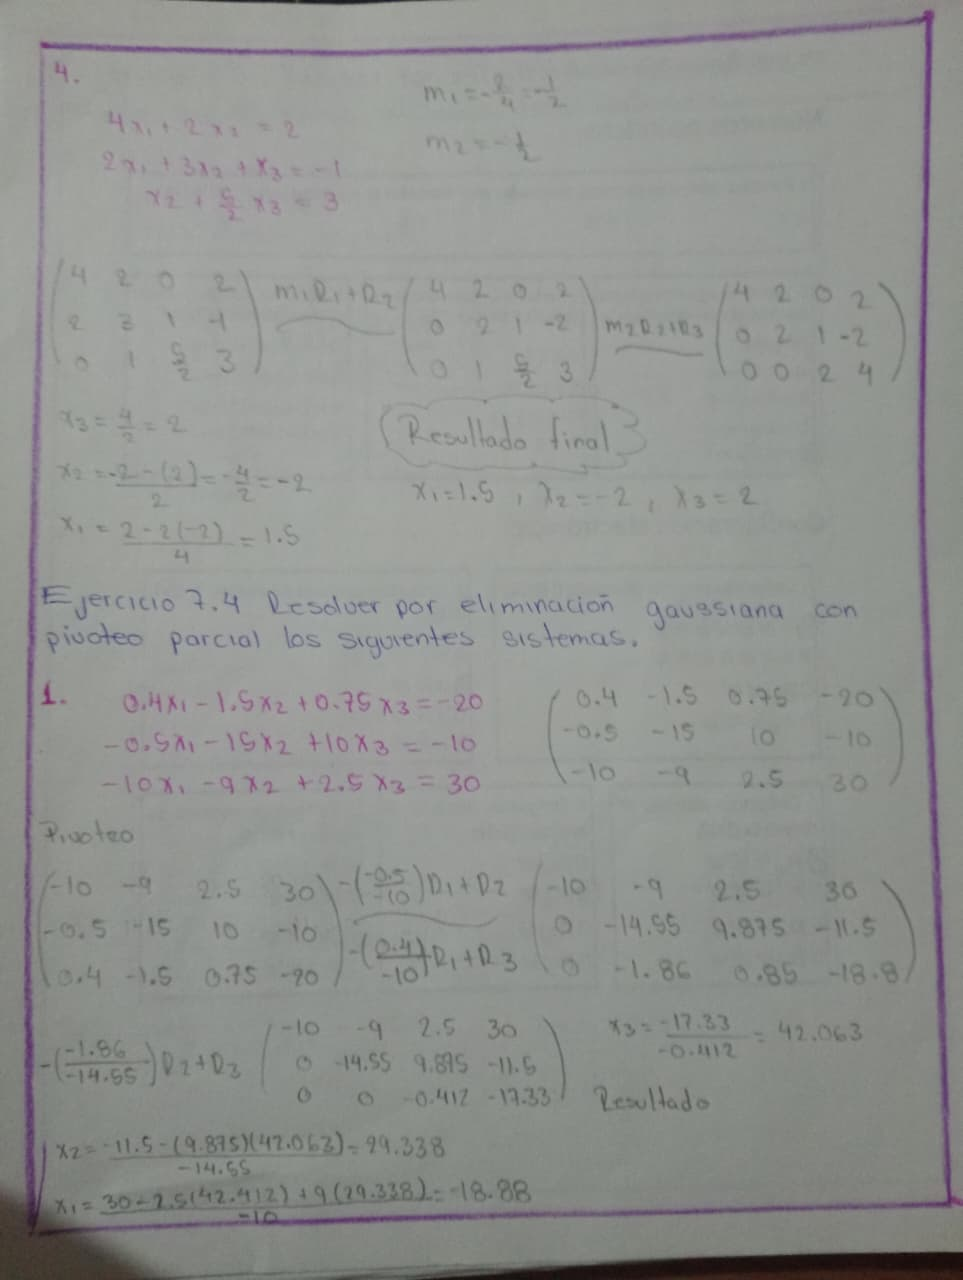
\includegraphics[width=2.60417in,height=\textheight,keepaspectratio,alt={pag.4}]{4.jpg}
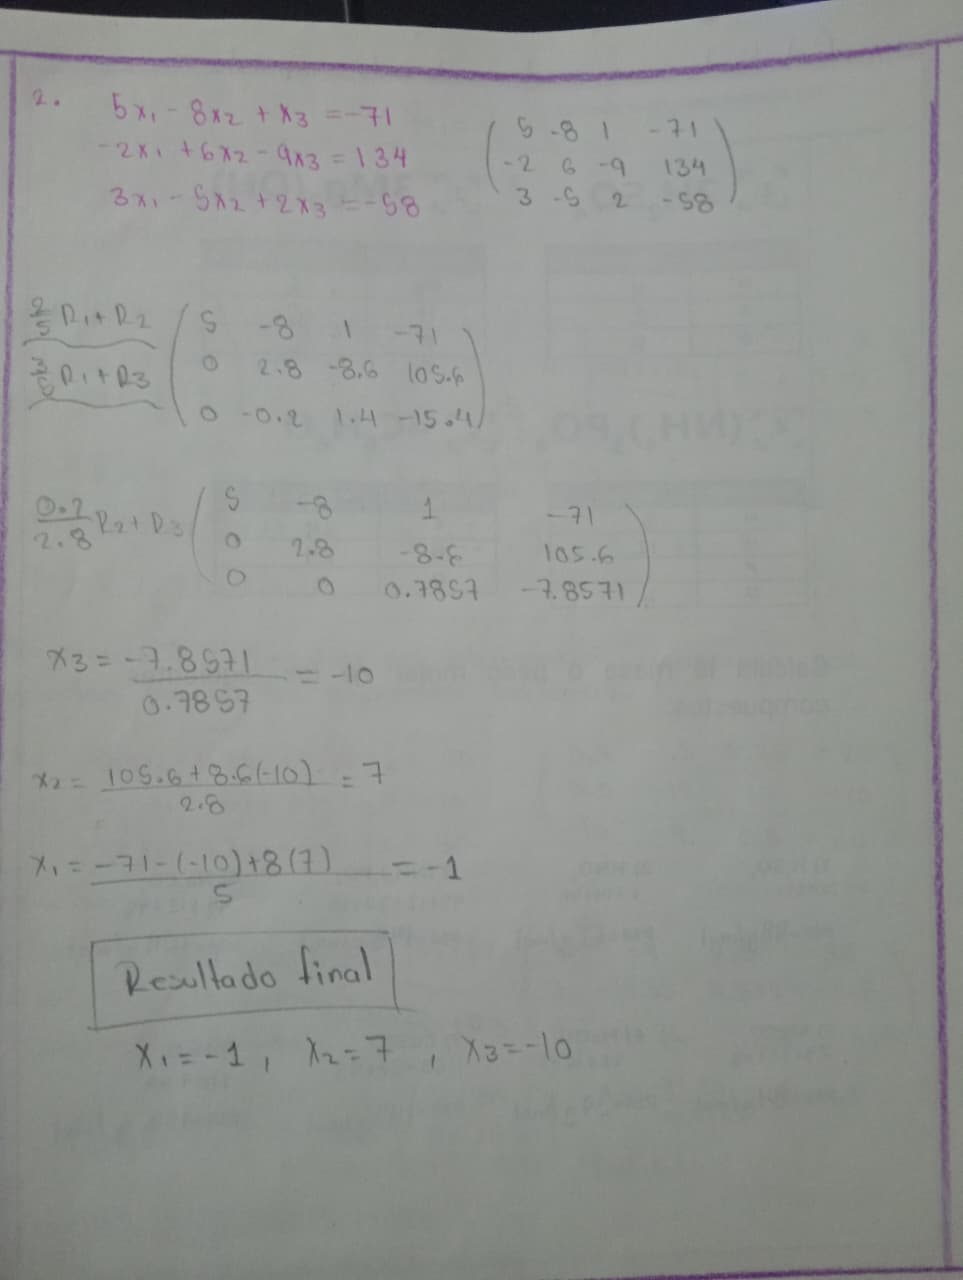
\includegraphics[width=2.60417in,height=\textheight,keepaspectratio,alt={pag.5}]{5.jpg}
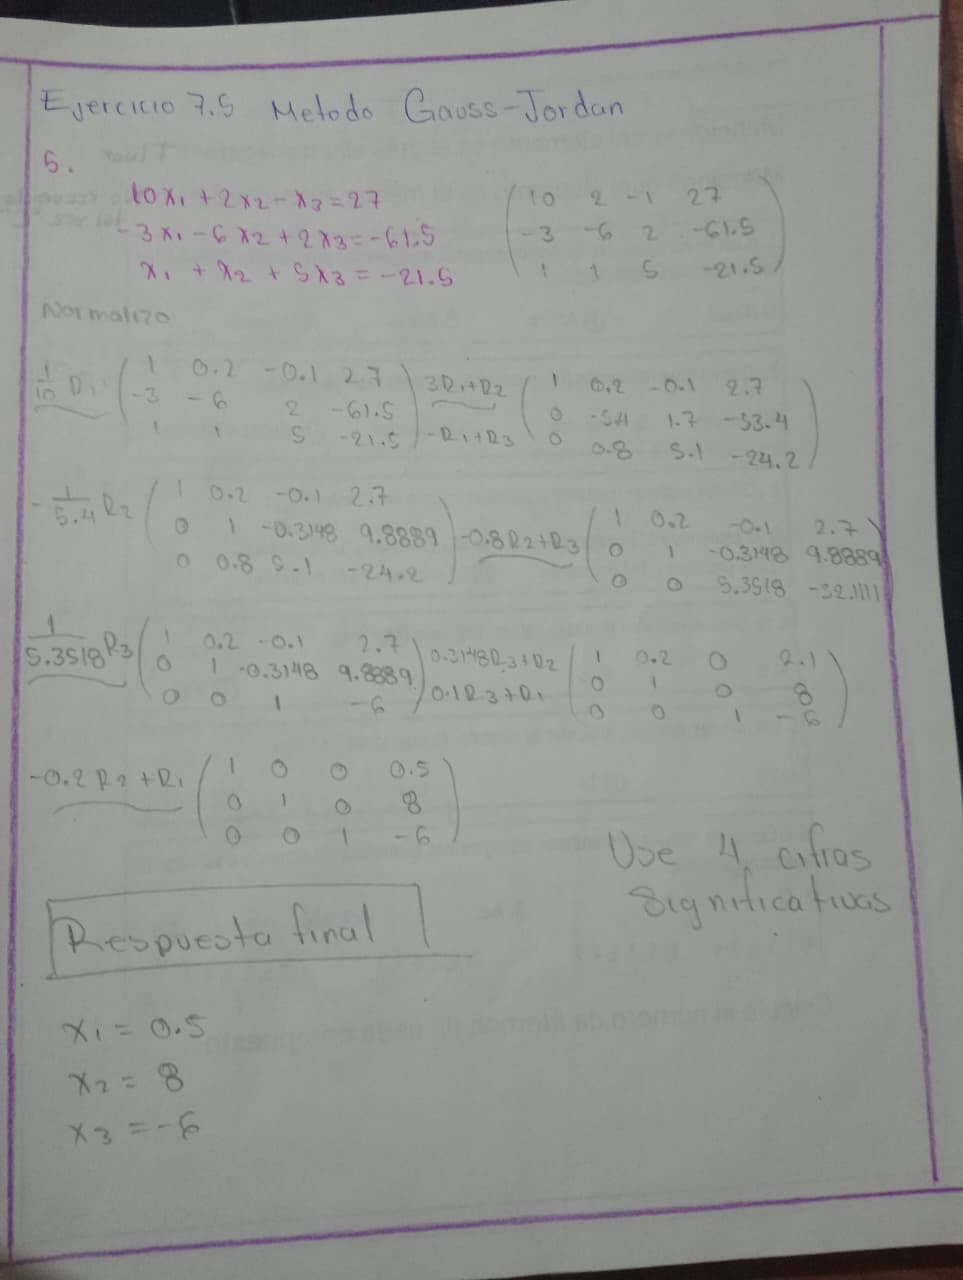
\includegraphics[width=2.60417in,height=\textheight,keepaspectratio,alt={pag.6}]{7.jpg}
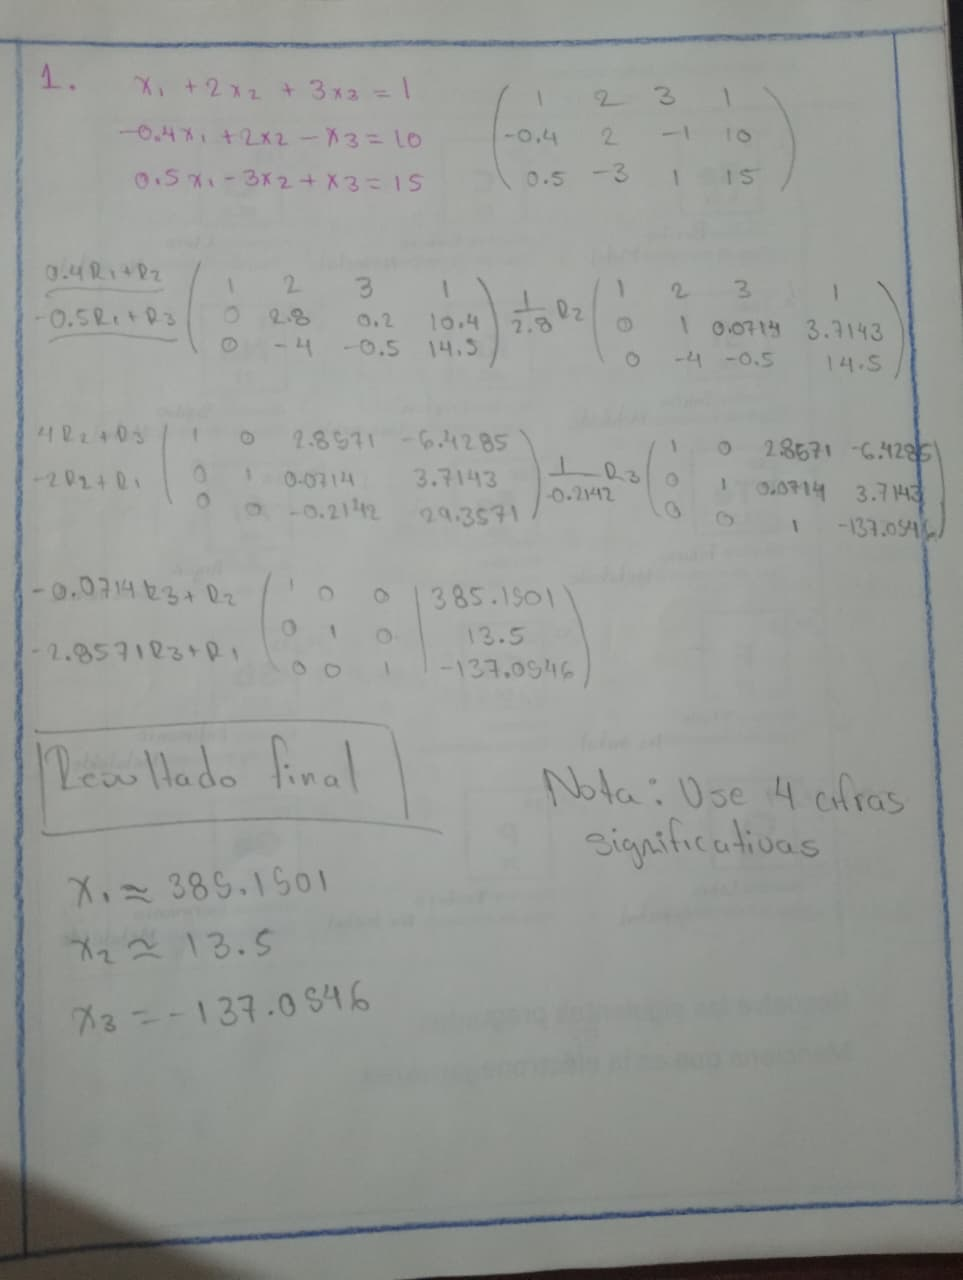
\includegraphics[width=2.60417in,height=\textheight,keepaspectratio,alt={pag.7}]{8.jpg}
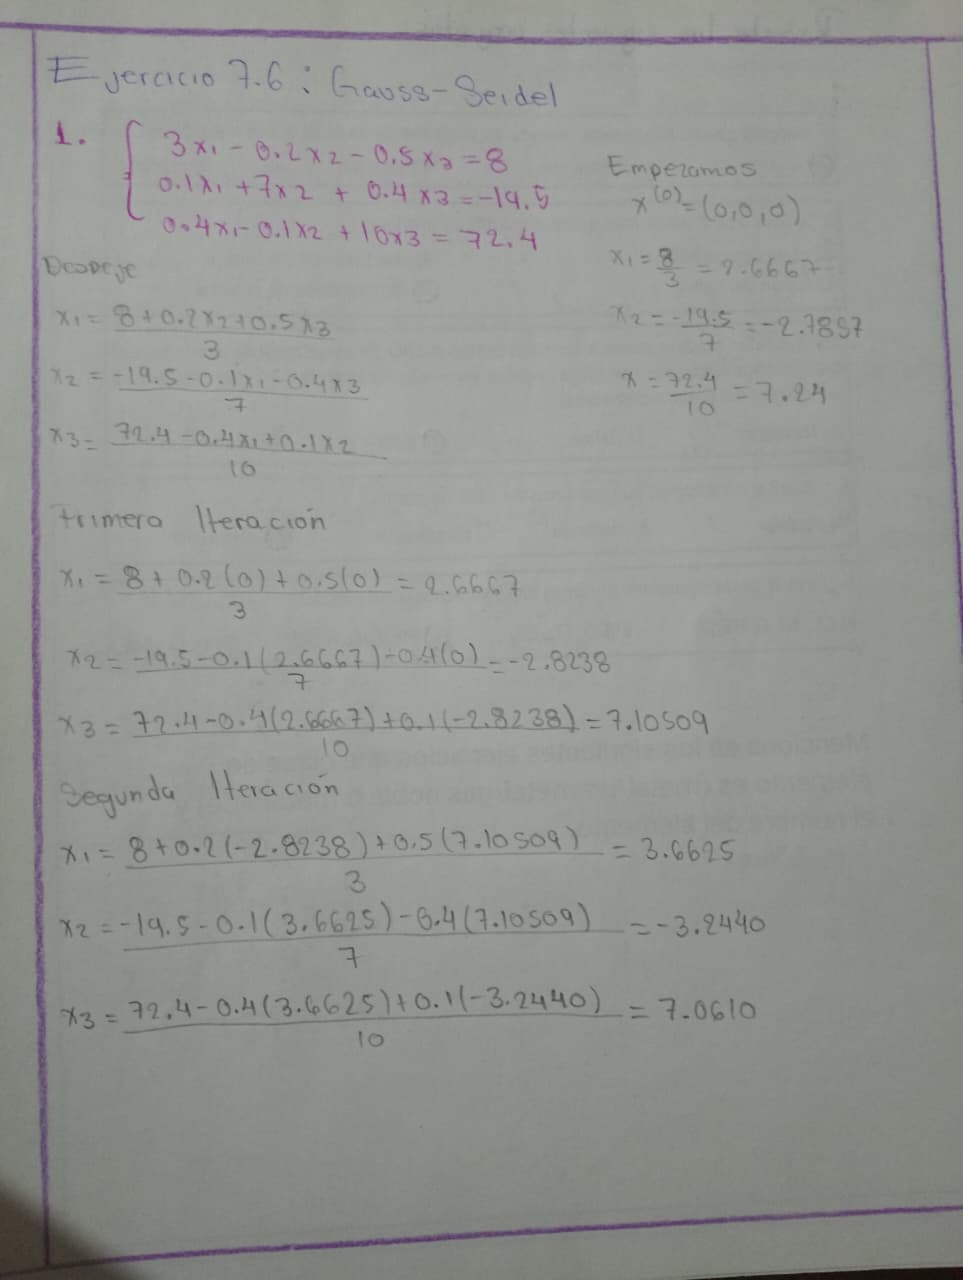
\includegraphics[width=2.60417in,height=\textheight,keepaspectratio,alt={pag.8}]{9.jpg}
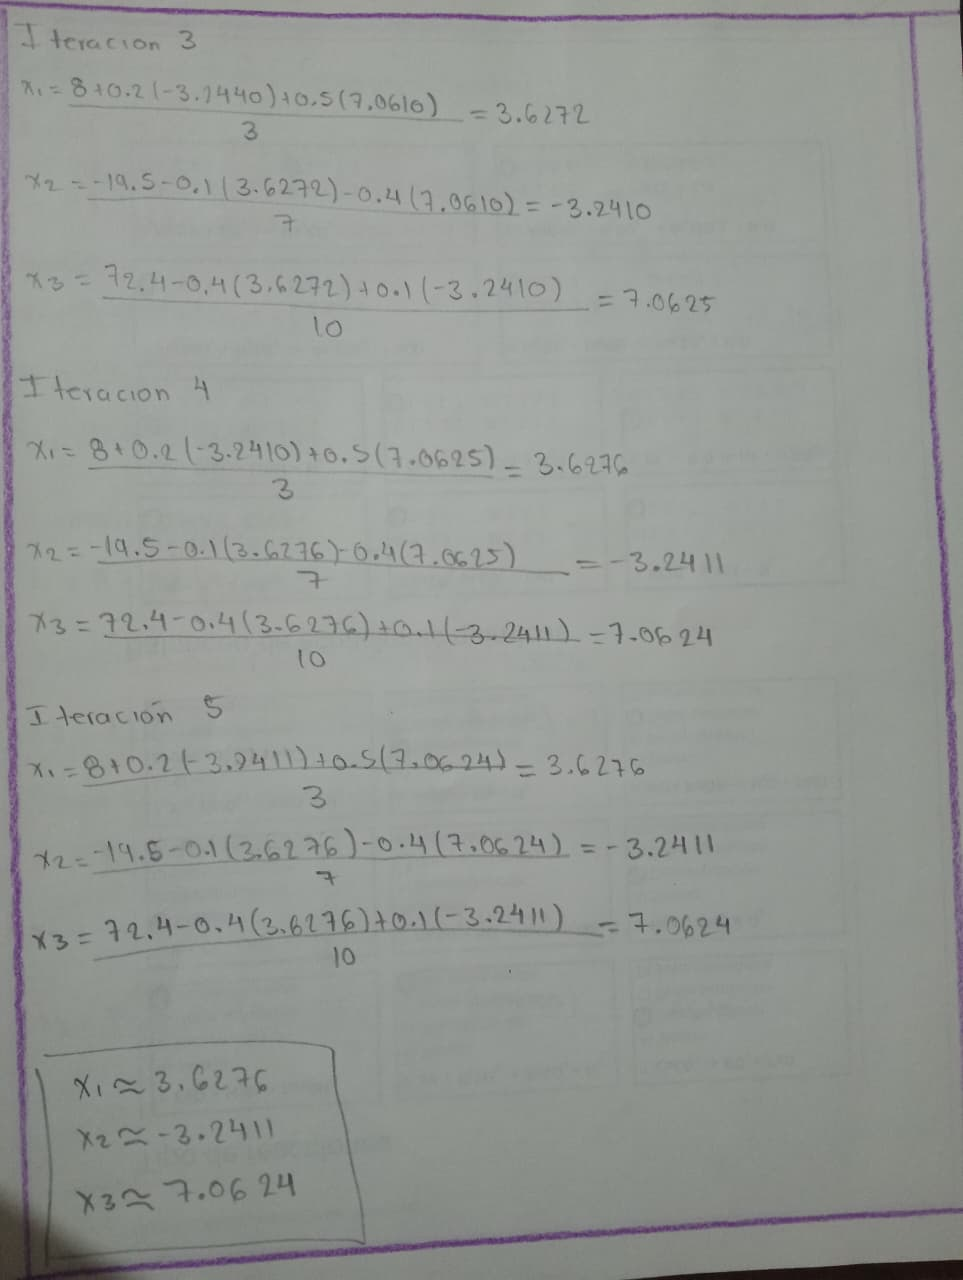
\includegraphics[width=2.60417in,height=\textheight,keepaspectratio,alt={pag.9}]{10.jpg}
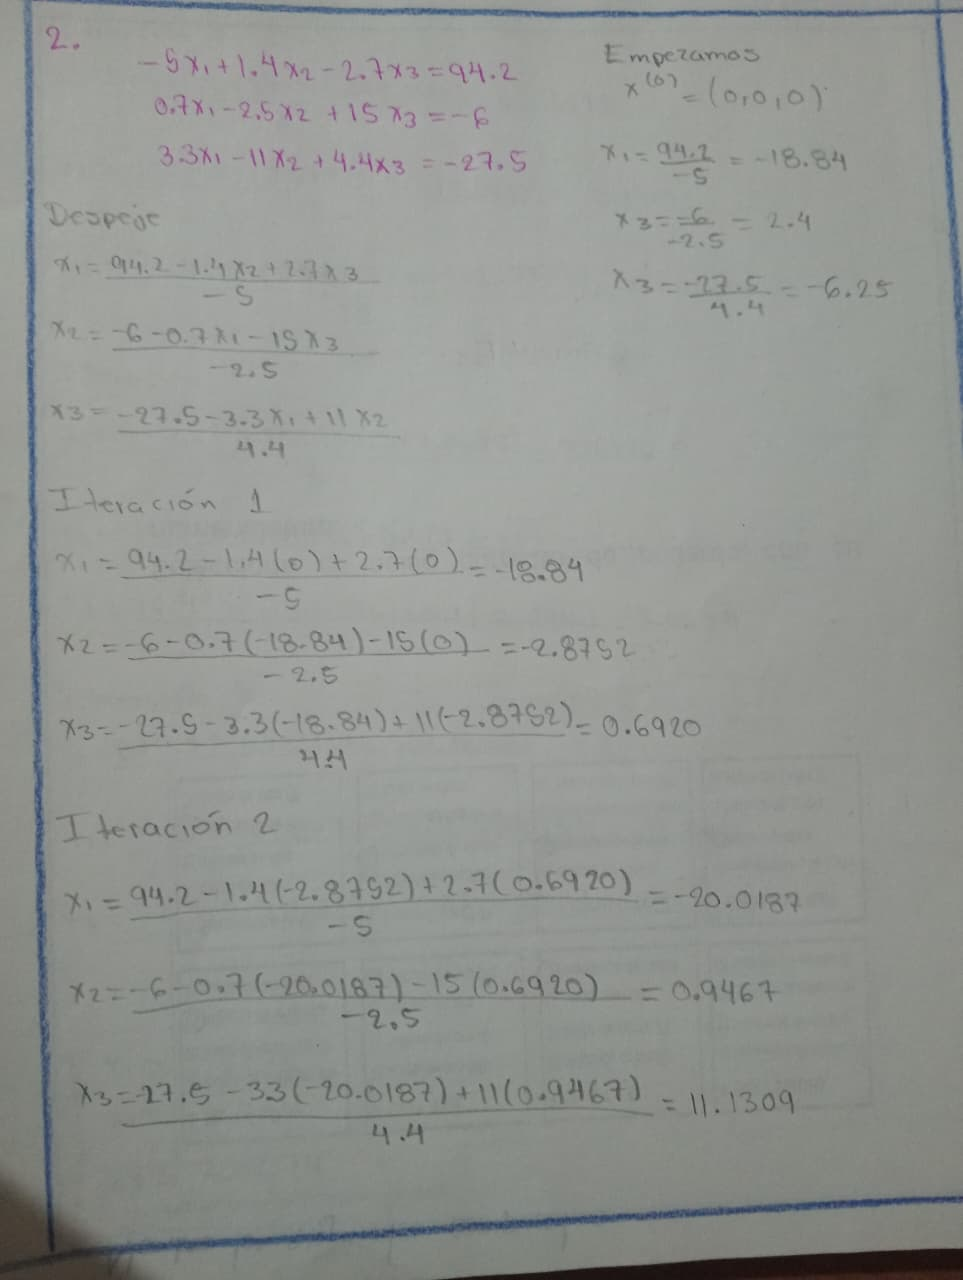
\includegraphics[width=2.60417in,height=\textheight,keepaspectratio,alt={pag.10}]{11.jpg}
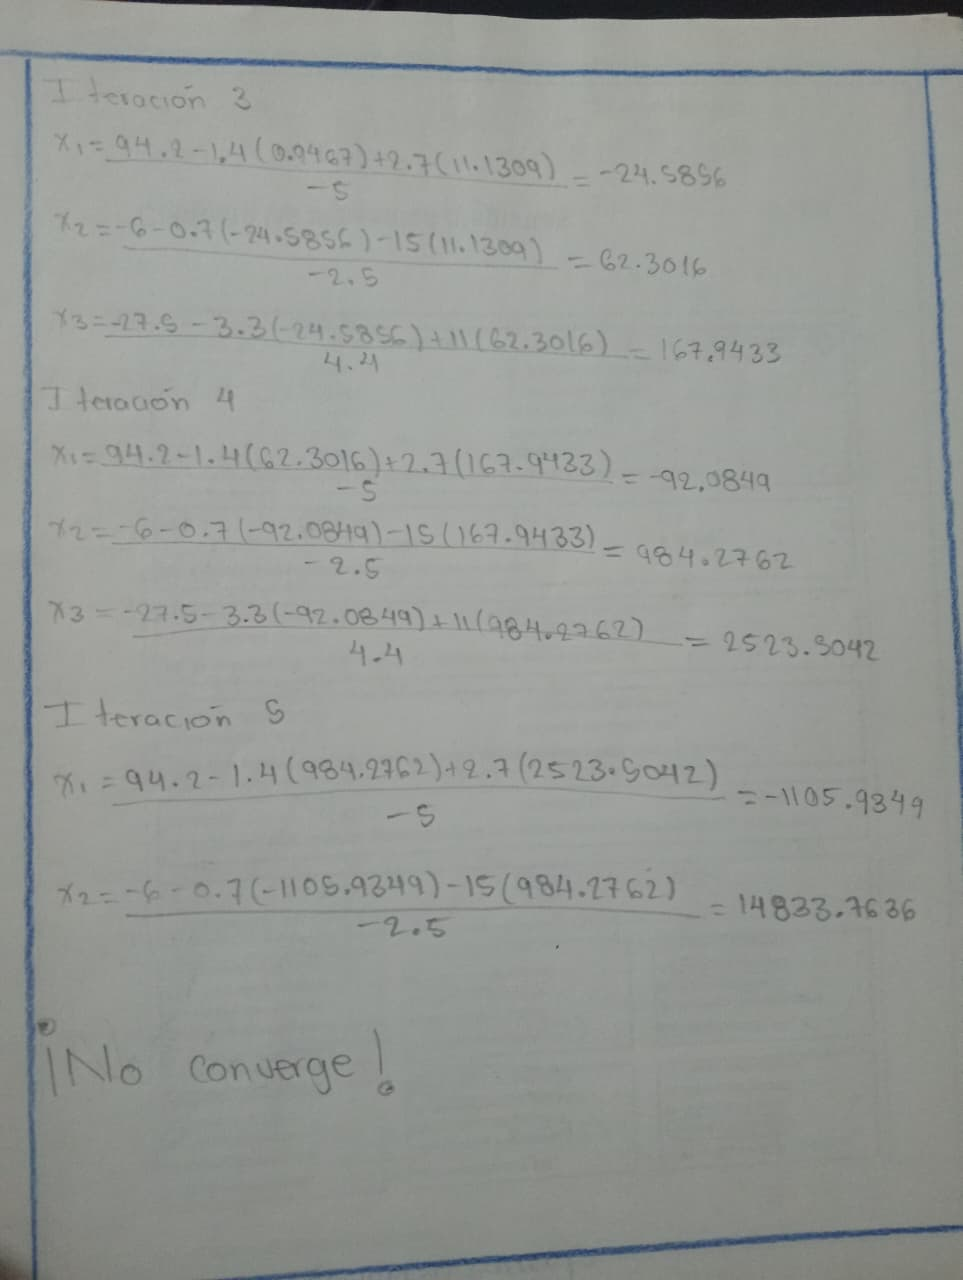
\includegraphics[width=2.60417in,height=\textheight,keepaspectratio,alt={pag.11}]{12.jpg}
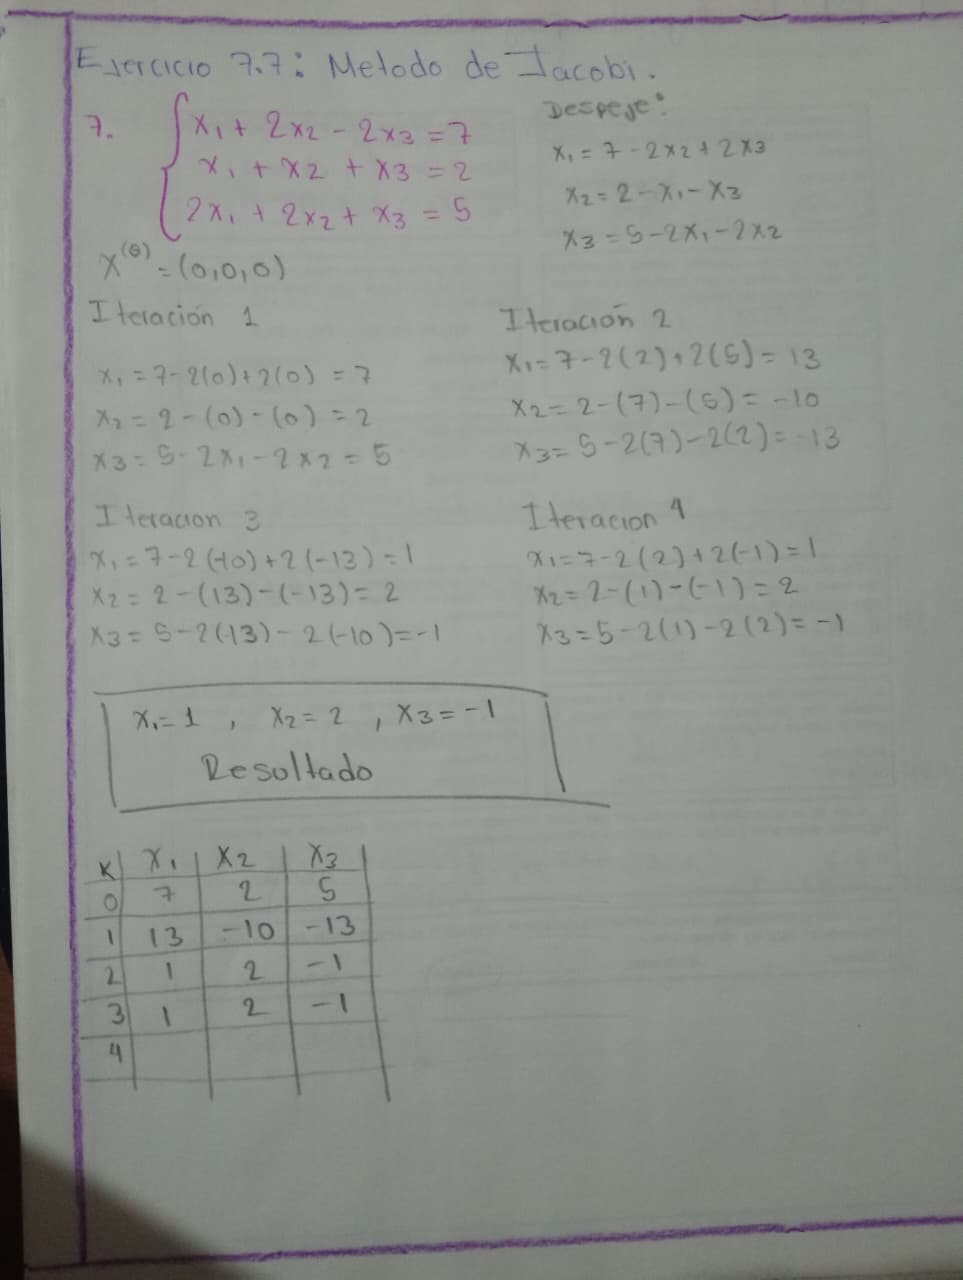
\includegraphics[width=2.60417in,height=\textheight,keepaspectratio,alt={pag.12}]{13.jpg}
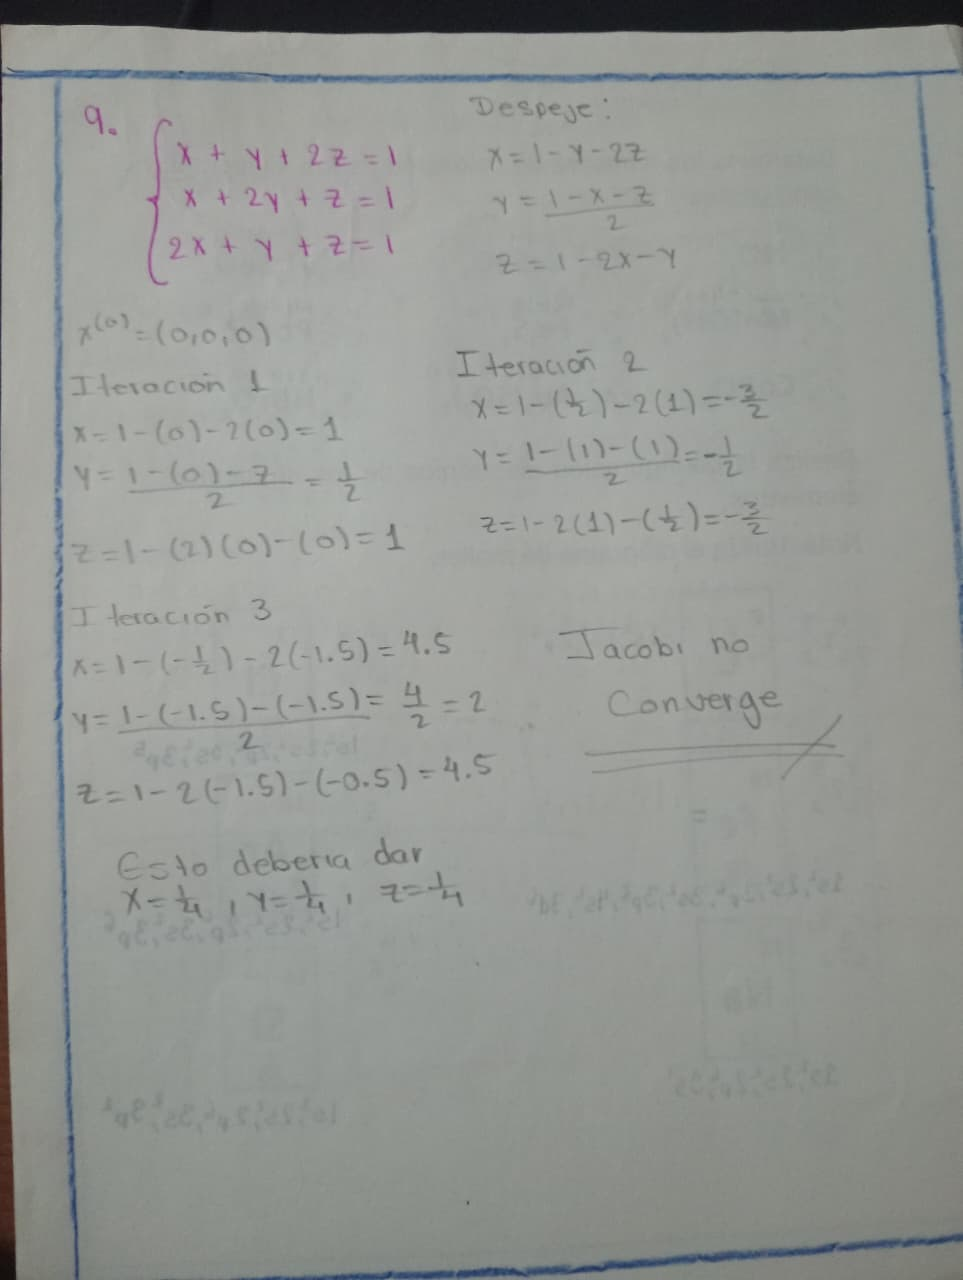
\includegraphics[width=2.60417in,height=\textheight,keepaspectratio,alt={pag.13}]{14.jpg}

\section{\texorpdfstring{\emph{Ejercicio 7.3. Eliminación Gaussiana
Simple}}{Ejercicio 7.3. Eliminación Gaussiana Simple}}\label{ejercicio-7.3.-eliminaciuxf3n-gaussiana-simple}

\subsection{7.3.1:}\label{section}

\(x_1−2x_2+0.5x_3 = −5\)

\(−2x_1+5x_2−1.5x_3 = 0\)

\(−0.2x_1+1.75x_2−x_3 = 10\)

\begin{Shaded}
\begin{Highlighting}[]
\NormalTok{ valoresc }\OtherTok{\textless{}{-}} \FunctionTok{c}\NormalTok{(}\DecValTok{1}\NormalTok{, }\SpecialCharTok{{-}}\DecValTok{2}\NormalTok{, }\SpecialCharTok{{-}}\FloatTok{0.2}\NormalTok{, }\SpecialCharTok{{-}}\DecValTok{2}\NormalTok{, }\DecValTok{5}\NormalTok{, }\FloatTok{1.75}\NormalTok{, }\FloatTok{0.5}\NormalTok{, }\SpecialCharTok{{-}}\FloatTok{1.5}\NormalTok{, }\SpecialCharTok{{-}}\DecValTok{1}\NormalTok{, }\SpecialCharTok{{-}}\DecValTok{5}\NormalTok{, }\DecValTok{0}\NormalTok{, }\DecValTok{10}\NormalTok{)}
\NormalTok{A}\OtherTok{\textless{}{-}} \FunctionTok{matrix}\NormalTok{(}\FunctionTok{t}\NormalTok{(valoresc), }\AttributeTok{nrow =} \DecValTok{3}\NormalTok{)}
\NormalTok{(A)}
\end{Highlighting}
\end{Shaded}

\begin{verbatim}
##      [,1]  [,2] [,3] [,4]
## [1,]  1.0 -2.00  0.5   -5
## [2,] -2.0  5.00 -1.5    0
## [3,] -0.2  1.75 -1.0   10
\end{verbatim}

\begin{Shaded}
\begin{Highlighting}[]
\NormalTok{m1 }\OtherTok{\textless{}{-}} \SpecialCharTok{{-}}\NormalTok{A[}\DecValTok{2}\NormalTok{,}\DecValTok{1}\NormalTok{]}\SpecialCharTok{/}\NormalTok{A[}\DecValTok{1}\NormalTok{,}\DecValTok{1}\NormalTok{]}
\NormalTok{m2 }\OtherTok{\textless{}{-}} \SpecialCharTok{{-}}\NormalTok{A[}\DecValTok{3}\NormalTok{,}\DecValTok{1}\NormalTok{]}\SpecialCharTok{/}\NormalTok{A[}\DecValTok{1}\NormalTok{,}\DecValTok{1}\NormalTok{]}
\NormalTok{R1 }\OtherTok{\textless{}{-}}\NormalTok{ A[}\DecValTok{1}\NormalTok{,]}
\NormalTok{R2}\OtherTok{\textless{}{-}}\NormalTok{ m1}\SpecialCharTok{*}\NormalTok{A[}\DecValTok{1}\NormalTok{,] }\SpecialCharTok{+}\NormalTok{ A[}\DecValTok{2}\NormalTok{,]}
\NormalTok{R3}\OtherTok{\textless{}{-}}\NormalTok{ m2}\SpecialCharTok{*}\NormalTok{A[}\DecValTok{1}\NormalTok{,] }\SpecialCharTok{+}\NormalTok{ A[}\DecValTok{3}\NormalTok{,]}
\NormalTok{A }\OtherTok{\textless{}{-}} \FunctionTok{rbind}\NormalTok{(R1, R2, R3)}
\FunctionTok{cat}\NormalTok{(}\StringTok{"Matriz después de la primera eliminación:}\SpecialCharTok{\textbackslash{}n}\StringTok{"}\NormalTok{)}
\end{Highlighting}
\end{Shaded}

\begin{verbatim}
## Matriz después de la primera eliminación:
\end{verbatim}

\begin{Shaded}
\begin{Highlighting}[]
\NormalTok{(A)}
\end{Highlighting}
\end{Shaded}

\begin{verbatim}
##    [,1]  [,2] [,3] [,4]
## R1    1 -2.00  0.5   -5
## R2    0  1.00 -0.5  -10
## R3    0  1.35 -0.9    9
\end{verbatim}

\begin{Shaded}
\begin{Highlighting}[]
\NormalTok{m3 }\OtherTok{\textless{}{-}} \SpecialCharTok{{-}}\NormalTok{A[}\DecValTok{3}\NormalTok{,}\DecValTok{2}\NormalTok{]}\SpecialCharTok{/}\NormalTok{A[}\DecValTok{2}\NormalTok{,}\DecValTok{2}\NormalTok{]}
\NormalTok{R1 }\OtherTok{\textless{}{-}}\NormalTok{ A[}\DecValTok{1}\NormalTok{,]}
\NormalTok{R2}\OtherTok{\textless{}{-}}\NormalTok{ A[}\DecValTok{2}\NormalTok{,]}
\NormalTok{R3}\OtherTok{\textless{}{-}}\NormalTok{ m3}\SpecialCharTok{*}\NormalTok{A[}\DecValTok{2}\NormalTok{,] }\SpecialCharTok{+}\NormalTok{ A[}\DecValTok{3}\NormalTok{,]}
\NormalTok{A }\OtherTok{\textless{}{-}} \FunctionTok{rbind}\NormalTok{(R1, R2, R3)}
\FunctionTok{cat}\NormalTok{(}\StringTok{"Matriz después de la segunda eliminación:}\SpecialCharTok{\textbackslash{}n}\StringTok{"}\NormalTok{)}
\end{Highlighting}
\end{Shaded}

\begin{verbatim}
## Matriz después de la segunda eliminación:
\end{verbatim}

\begin{Shaded}
\begin{Highlighting}[]
\NormalTok{(A)}
\end{Highlighting}
\end{Shaded}

\begin{verbatim}
##    [,1] [,2]   [,3]  [,4]
## R1    1   -2  0.500  -5.0
## R2    0    1 -0.500 -10.0
## R3    0    0 -0.225  22.5
\end{verbatim}

\paragraph{resultado final:}\label{resultado-final}

\begin{Shaded}
\begin{Highlighting}[]
\NormalTok{x3 }\OtherTok{\textless{}{-}}\NormalTok{ A[}\DecValTok{3}\NormalTok{,}\DecValTok{4}\NormalTok{] }\SpecialCharTok{/}\NormalTok{ A[}\DecValTok{3}\NormalTok{,}\DecValTok{3}\NormalTok{]}
\NormalTok{x2 }\OtherTok{\textless{}{-}}\NormalTok{ (A[}\DecValTok{2}\NormalTok{,}\DecValTok{4}\NormalTok{]}\SpecialCharTok{{-}}\NormalTok{ (A[}\DecValTok{2}\NormalTok{,}\DecValTok{3}\NormalTok{]}\SpecialCharTok{*}\NormalTok{x3))}\SpecialCharTok{/}\NormalTok{ A[}\DecValTok{2}\NormalTok{,}\DecValTok{2}\NormalTok{] }
\NormalTok{x1 }\OtherTok{\textless{}{-}}\NormalTok{ (A[}\DecValTok{1}\NormalTok{,}\DecValTok{4}\NormalTok{]}\SpecialCharTok{{-}}\NormalTok{(A[}\DecValTok{1}\NormalTok{,}\DecValTok{3}\NormalTok{]}\SpecialCharTok{*}\NormalTok{x3) }\SpecialCharTok{{-}}\NormalTok{ (A[}\DecValTok{1}\NormalTok{,}\DecValTok{2}\NormalTok{]}\SpecialCharTok{*}\NormalTok{x2))}\SpecialCharTok{/}\NormalTok{ A[}\DecValTok{1}\NormalTok{,}\DecValTok{1}\NormalTok{]}
\FunctionTok{cat}\NormalTok{(}\StringTok{"Soluciones del sistema:}\SpecialCharTok{\textbackslash{}n}\StringTok{"}\NormalTok{)}
\end{Highlighting}
\end{Shaded}

\begin{verbatim}
## Soluciones del sistema:
\end{verbatim}

\begin{Shaded}
\begin{Highlighting}[]
\FunctionTok{cat}\NormalTok{(}\StringTok{"x1 ="}\NormalTok{, x1, }\StringTok{"}\SpecialCharTok{\textbackslash{}n}\StringTok{"}\NormalTok{)}
\end{Highlighting}
\end{Shaded}

\begin{verbatim}
## x1 = -75
\end{verbatim}

\begin{Shaded}
\begin{Highlighting}[]
\FunctionTok{cat}\NormalTok{(}\StringTok{"x2 ="}\NormalTok{, x2, }\StringTok{"}\SpecialCharTok{\textbackslash{}n}\StringTok{"}\NormalTok{) }
\end{Highlighting}
\end{Shaded}

\begin{verbatim}
## x2 = -60
\end{verbatim}

\begin{Shaded}
\begin{Highlighting}[]
\FunctionTok{cat}\NormalTok{(}\StringTok{"x3 ="}\NormalTok{, x3, }\StringTok{"}\SpecialCharTok{\textbackslash{}n}\StringTok{"}\NormalTok{)}
\end{Highlighting}
\end{Shaded}

\begin{verbatim}
## x3 = -100
\end{verbatim}

\subsection{7.3.2:}\label{section-1}

\(3x_1−x_2+6x_4 = 2.3\)

\(4x_1+2x_2−x_3−5x_4 = 6.9\)

\(−5x_1+x_2−3x_3 = −36\)

\(10x_2−4x_3+7x_4 = −36\)

\begin{Shaded}
\begin{Highlighting}[]
\NormalTok{ valoresc }\OtherTok{\textless{}{-}} \FunctionTok{c}\NormalTok{(}\DecValTok{3}\NormalTok{, }\DecValTok{4}\NormalTok{,}\SpecialCharTok{{-}}\DecValTok{5}\NormalTok{, }\DecValTok{0}\NormalTok{, }\SpecialCharTok{{-}}\DecValTok{1}\NormalTok{, }\DecValTok{2}\NormalTok{,}\DecValTok{1}\NormalTok{, }\DecValTok{10}\NormalTok{,}\DecValTok{0}\NormalTok{, }\SpecialCharTok{{-}}\DecValTok{1}\NormalTok{,}\SpecialCharTok{{-}}\DecValTok{3}\NormalTok{, }\SpecialCharTok{{-}}\DecValTok{4}\NormalTok{, }\DecValTok{6}\NormalTok{, }\SpecialCharTok{{-}}\DecValTok{5}\NormalTok{, }\DecValTok{0}\NormalTok{, }\DecValTok{7}\NormalTok{, }\FloatTok{2.3}\NormalTok{, }\FloatTok{6.9}\NormalTok{, }\SpecialCharTok{{-}}\DecValTok{36}\NormalTok{, }\SpecialCharTok{{-}}\DecValTok{36}\NormalTok{)}
\NormalTok{A}\OtherTok{\textless{}{-}} \FunctionTok{matrix}\NormalTok{(}\FunctionTok{t}\NormalTok{(valoresc), }\AttributeTok{nrow =} \DecValTok{4}\NormalTok{)}
\NormalTok{(A)}
\end{Highlighting}
\end{Shaded}

\begin{verbatim}
##      [,1] [,2] [,3] [,4]  [,5]
## [1,]    3   -1    0    6   2.3
## [2,]    4    2   -1   -5   6.9
## [3,]   -5    1   -3    0 -36.0
## [4,]    0   10   -4    7 -36.0
\end{verbatim}

\begin{Shaded}
\begin{Highlighting}[]
\NormalTok{m1 }\OtherTok{\textless{}{-}} \SpecialCharTok{{-}}\NormalTok{A[}\DecValTok{2}\NormalTok{,}\DecValTok{1}\NormalTok{]}\SpecialCharTok{/}\NormalTok{A[}\DecValTok{1}\NormalTok{,}\DecValTok{1}\NormalTok{]}
\NormalTok{m2 }\OtherTok{\textless{}{-}} \SpecialCharTok{{-}}\NormalTok{A[}\DecValTok{3}\NormalTok{,}\DecValTok{1}\NormalTok{]}\SpecialCharTok{/}\NormalTok{A[}\DecValTok{1}\NormalTok{,}\DecValTok{1}\NormalTok{]}
\NormalTok{m3 }\OtherTok{\textless{}{-}} \SpecialCharTok{{-}}\NormalTok{A[}\DecValTok{4}\NormalTok{,}\DecValTok{1}\NormalTok{]}\SpecialCharTok{/}\NormalTok{A[}\DecValTok{1}\NormalTok{,}\DecValTok{1}\NormalTok{]}
\NormalTok{R1 }\OtherTok{\textless{}{-}}\NormalTok{ A[}\DecValTok{1}\NormalTok{,]}
\NormalTok{R2}\OtherTok{\textless{}{-}}\NormalTok{ m1}\SpecialCharTok{*}\NormalTok{A[}\DecValTok{1}\NormalTok{,] }\SpecialCharTok{+}\NormalTok{ A[}\DecValTok{2}\NormalTok{,]}
\NormalTok{R3}\OtherTok{\textless{}{-}}\NormalTok{ m2}\SpecialCharTok{*}\NormalTok{A[}\DecValTok{1}\NormalTok{,] }\SpecialCharTok{+}\NormalTok{ A[}\DecValTok{3}\NormalTok{,]}
\NormalTok{R4}\OtherTok{\textless{}{-}}\NormalTok{ m3}\SpecialCharTok{*}\NormalTok{A[}\DecValTok{1}\NormalTok{,] }\SpecialCharTok{+}\NormalTok{ A[}\DecValTok{4}\NormalTok{,]}
\NormalTok{A }\OtherTok{\textless{}{-}} \FunctionTok{rbind}\NormalTok{(R1, R2, R3,R4)}
\FunctionTok{cat}\NormalTok{(}\StringTok{"Matriz después de primera eliminación:}\SpecialCharTok{\textbackslash{}n}\StringTok{"}\NormalTok{)}
\end{Highlighting}
\end{Shaded}

\begin{verbatim}
## Matriz después de primera eliminación:
\end{verbatim}

\begin{Shaded}
\begin{Highlighting}[]
\NormalTok{(A)}
\end{Highlighting}
\end{Shaded}

\begin{verbatim}
##    [,1]       [,2] [,3] [,4]       [,5]
## R1    3 -1.0000000    0    6   2.300000
## R2    0  3.3333333   -1  -13   3.833333
## R3    0 -0.6666667   -3   10 -32.166667
## R4    0 10.0000000   -4    7 -36.000000
\end{verbatim}

\begin{Shaded}
\begin{Highlighting}[]
\NormalTok{m4 }\OtherTok{\textless{}{-}} \SpecialCharTok{{-}}\NormalTok{A[}\DecValTok{3}\NormalTok{,}\DecValTok{2}\NormalTok{]}\SpecialCharTok{/}\NormalTok{A[}\DecValTok{2}\NormalTok{,}\DecValTok{2}\NormalTok{]}
\NormalTok{m5 }\OtherTok{\textless{}{-}} \SpecialCharTok{{-}}\NormalTok{A[}\DecValTok{4}\NormalTok{,}\DecValTok{2}\NormalTok{]}\SpecialCharTok{/}\NormalTok{A[}\DecValTok{2}\NormalTok{,}\DecValTok{2}\NormalTok{]}
\NormalTok{R1 }\OtherTok{\textless{}{-}}\NormalTok{ A[}\DecValTok{1}\NormalTok{,]}
\NormalTok{R2}\OtherTok{\textless{}{-}}\NormalTok{ A[}\DecValTok{2}\NormalTok{,]}
\NormalTok{R3}\OtherTok{\textless{}{-}}\NormalTok{ m4}\SpecialCharTok{*}\NormalTok{A[}\DecValTok{2}\NormalTok{,] }\SpecialCharTok{+}\NormalTok{ A[}\DecValTok{3}\NormalTok{,]}
\NormalTok{R4}\OtherTok{\textless{}{-}}\NormalTok{ m5}\SpecialCharTok{*}\NormalTok{A[}\DecValTok{2}\NormalTok{,] }\SpecialCharTok{+}\NormalTok{ A[}\DecValTok{4}\NormalTok{,]}
\NormalTok{A }\OtherTok{\textless{}{-}} \FunctionTok{rbind}\NormalTok{(R1, R2, R3,R4)}
\FunctionTok{cat}\NormalTok{(}\StringTok{"Matriz después de la segunda eliminación:}\SpecialCharTok{\textbackslash{}n}\StringTok{"}\NormalTok{)}
\end{Highlighting}
\end{Shaded}

\begin{verbatim}
## Matriz después de la segunda eliminación:
\end{verbatim}

\begin{Shaded}
\begin{Highlighting}[]
\NormalTok{(A)}
\end{Highlighting}
\end{Shaded}

\begin{verbatim}
##    [,1]      [,2] [,3]  [,4]       [,5]
## R1    3 -1.000000  0.0   6.0   2.300000
## R2    0  3.333333 -1.0 -13.0   3.833333
## R3    0  0.000000 -3.2   7.4 -31.400000
## R4    0  0.000000 -1.0  46.0 -47.500000
\end{verbatim}

\begin{Shaded}
\begin{Highlighting}[]
\NormalTok{m6 }\OtherTok{\textless{}{-}} \SpecialCharTok{{-}}\NormalTok{A[}\DecValTok{4}\NormalTok{,}\DecValTok{3}\NormalTok{]}\SpecialCharTok{/}\NormalTok{A[}\DecValTok{3}\NormalTok{,}\DecValTok{3}\NormalTok{]}
\NormalTok{R1 }\OtherTok{\textless{}{-}}\NormalTok{ A[}\DecValTok{1}\NormalTok{,]}
\NormalTok{R2}\OtherTok{\textless{}{-}}\NormalTok{ A[}\DecValTok{2}\NormalTok{,]}
\NormalTok{R3}\OtherTok{\textless{}{-}}\NormalTok{ A[}\DecValTok{3}\NormalTok{,]}
\NormalTok{R4}\OtherTok{\textless{}{-}}\NormalTok{ m6}\SpecialCharTok{*}\NormalTok{A[}\DecValTok{3}\NormalTok{,] }\SpecialCharTok{+}\NormalTok{ A[}\DecValTok{4}\NormalTok{,]}
\NormalTok{A }\OtherTok{\textless{}{-}} \FunctionTok{rbind}\NormalTok{(R1, R2, R3,R4)}
\FunctionTok{cat}\NormalTok{(}\StringTok{"Matriz después de la eliminación:}\SpecialCharTok{\textbackslash{}n}\StringTok{"}\NormalTok{)}
\end{Highlighting}
\end{Shaded}

\begin{verbatim}
## Matriz después de la eliminación:
\end{verbatim}

\begin{Shaded}
\begin{Highlighting}[]
\NormalTok{(A)}
\end{Highlighting}
\end{Shaded}

\begin{verbatim}
##    [,1]      [,2] [,3]     [,4]       [,5]
## R1    3 -1.000000  0.0   6.0000   2.300000
## R2    0  3.333333 -1.0 -13.0000   3.833333
## R3    0  0.000000 -3.2   7.4000 -31.400000
## R4    0  0.000000  0.0  43.6875 -37.687500
\end{verbatim}

\subsubsection{resultado final:}\label{resultado-final-1}

\begin{Shaded}
\begin{Highlighting}[]
\NormalTok{x4 }\OtherTok{\textless{}{-}}\NormalTok{ A[}\DecValTok{4}\NormalTok{,}\DecValTok{5}\NormalTok{] }\SpecialCharTok{/}\NormalTok{ A[}\DecValTok{4}\NormalTok{,}\DecValTok{4}\NormalTok{]}
\NormalTok{x3 }\OtherTok{\textless{}{-}}\NormalTok{ (A[}\DecValTok{3}\NormalTok{,}\DecValTok{5}\NormalTok{]}\SpecialCharTok{{-}}\NormalTok{(A[}\DecValTok{3}\NormalTok{,}\DecValTok{4}\NormalTok{] }\SpecialCharTok{*}\NormalTok{ x4)) }\SpecialCharTok{/}\NormalTok{ A[}\DecValTok{3}\NormalTok{,}\DecValTok{3}\NormalTok{]}
\NormalTok{x2 }\OtherTok{\textless{}{-}}\NormalTok{ (A[}\DecValTok{2}\NormalTok{,}\DecValTok{5}\NormalTok{]}\SpecialCharTok{{-}}\NormalTok{ (A[}\DecValTok{2}\NormalTok{,}\DecValTok{4}\NormalTok{]}\SpecialCharTok{*}\NormalTok{x4)}\SpecialCharTok{{-}}\NormalTok{(A[}\DecValTok{2}\NormalTok{,}\DecValTok{3}\NormalTok{]}\SpecialCharTok{*}\NormalTok{x3 ))}\SpecialCharTok{/}\NormalTok{ A[}\DecValTok{2}\NormalTok{,}\DecValTok{2}\NormalTok{] }
\NormalTok{x1 }\OtherTok{\textless{}{-}}\NormalTok{ (A[}\DecValTok{1}\NormalTok{,}\DecValTok{5}\NormalTok{]}\SpecialCharTok{{-}}\NormalTok{(A[}\DecValTok{1}\NormalTok{,}\DecValTok{4}\NormalTok{]}\SpecialCharTok{*}\NormalTok{x4) }\SpecialCharTok{{-}}\NormalTok{ (A[}\DecValTok{1}\NormalTok{,}\DecValTok{3}\NormalTok{]}\SpecialCharTok{*}\NormalTok{x3)}\SpecialCharTok{{-}}\NormalTok{(A[}\DecValTok{1}\NormalTok{,}\DecValTok{2}\NormalTok{]}\SpecialCharTok{*}\NormalTok{x2))}\SpecialCharTok{/}\NormalTok{ A[}\DecValTok{1}\NormalTok{,}\DecValTok{1}\NormalTok{]}
\FunctionTok{cat}\NormalTok{(}\StringTok{"Soluciones del sistema:}\SpecialCharTok{\textbackslash{}n}\StringTok{"}\NormalTok{)}
\end{Highlighting}
\end{Shaded}

\begin{verbatim}
## Soluciones del sistema:
\end{verbatim}

\begin{Shaded}
\begin{Highlighting}[]
\FunctionTok{cat}\NormalTok{(}\StringTok{"x1 ="}\NormalTok{, x1, }\StringTok{"}\SpecialCharTok{\textbackslash{}n}\StringTok{"}\NormalTok{)}
\end{Highlighting}
\end{Shaded}

\begin{verbatim}
## x1 = 2.535622
\end{verbatim}

\begin{Shaded}
\begin{Highlighting}[]
\FunctionTok{cat}\NormalTok{(}\StringTok{"x2 ="}\NormalTok{, x2, }\StringTok{"}\SpecialCharTok{\textbackslash{}n}\StringTok{"}\NormalTok{) }
\end{Highlighting}
\end{Shaded}

\begin{verbatim}
## x2 = 0.1309013
\end{verbatim}

\begin{Shaded}
\begin{Highlighting}[]
\FunctionTok{cat}\NormalTok{(}\StringTok{"x3 ="}\NormalTok{, x3, }\StringTok{"}\SpecialCharTok{\textbackslash{}n}\StringTok{"}\NormalTok{)}
\end{Highlighting}
\end{Shaded}

\begin{verbatim}
## x3 = 7.817597
\end{verbatim}

\begin{Shaded}
\begin{Highlighting}[]
\FunctionTok{cat}\NormalTok{(}\StringTok{"x4 ="}\NormalTok{, x4, }\StringTok{"}\SpecialCharTok{\textbackslash{}n}\StringTok{"}\NormalTok{)}
\end{Highlighting}
\end{Shaded}

\begin{verbatim}
## x4 = -0.8626609
\end{verbatim}

\subsection{7.3.3:}\label{section-2}

\(0.003000x_1+59.14x_2 = 59.17\)

\(5.291x_1−6.130x_2 = 46.78\)

\begin{Shaded}
\begin{Highlighting}[]
\NormalTok{valoresc }\OtherTok{\textless{}{-}} \FunctionTok{c}\NormalTok{(}\FloatTok{0.003000}\NormalTok{, }\FloatTok{5.291}\NormalTok{, }\FloatTok{59.14}\NormalTok{,}\SpecialCharTok{{-}}\FloatTok{6.130}\NormalTok{, }\FloatTok{59.17}\NormalTok{, }\FloatTok{46.78}\NormalTok{)}
\NormalTok{A}\OtherTok{\textless{}{-}} \FunctionTok{matrix}\NormalTok{(}\FunctionTok{t}\NormalTok{(valoresc), }\AttributeTok{nrow =} \DecValTok{2}\NormalTok{)}
\NormalTok{(A)}
\end{Highlighting}
\end{Shaded}

\begin{verbatim}
##       [,1]  [,2]  [,3]
## [1,] 0.003 59.14 59.17
## [2,] 5.291 -6.13 46.78
\end{verbatim}

\begin{Shaded}
\begin{Highlighting}[]
\NormalTok{m1 }\OtherTok{\textless{}{-}} \SpecialCharTok{{-}}\NormalTok{A[}\DecValTok{2}\NormalTok{,}\DecValTok{1}\NormalTok{]}\SpecialCharTok{/}\NormalTok{A[}\DecValTok{1}\NormalTok{,}\DecValTok{1}\NormalTok{]}
\NormalTok{R1 }\OtherTok{\textless{}{-}}\NormalTok{ A[}\DecValTok{1}\NormalTok{,]}
\NormalTok{R2}\OtherTok{\textless{}{-}}\NormalTok{ m1}\SpecialCharTok{*}\NormalTok{A[}\DecValTok{1}\NormalTok{,] }\SpecialCharTok{+}\NormalTok{ A[}\DecValTok{2}\NormalTok{,]}
\NormalTok{A }\OtherTok{\textless{}{-}} \FunctionTok{rbind}\NormalTok{(R1, R2)}
\FunctionTok{cat}\NormalTok{(}\StringTok{"Matriz después de primera eliminación:}\SpecialCharTok{\textbackslash{}n}\StringTok{"}\NormalTok{)}
\end{Highlighting}
\end{Shaded}

\begin{verbatim}
## Matriz después de primera eliminación:
\end{verbatim}

\begin{Shaded}
\begin{Highlighting}[]
\NormalTok{(A)}
\end{Highlighting}
\end{Shaded}

\begin{verbatim}
##     [,1]       [,2]       [,3]
## R1 0.003      59.14      59.17
## R2 0.000 -104309.38 -104309.38
\end{verbatim}

\subsubsection{resultado final:}\label{resultado-final-2}

\begin{Shaded}
\begin{Highlighting}[]
\NormalTok{x2 }\OtherTok{\textless{}{-}}\NormalTok{ A[}\DecValTok{2}\NormalTok{,}\DecValTok{3}\NormalTok{] }\SpecialCharTok{/}\NormalTok{ A[}\DecValTok{2}\NormalTok{,}\DecValTok{2}\NormalTok{]}
\NormalTok{x1 }\OtherTok{\textless{}{-}}\NormalTok{ (A[}\DecValTok{1}\NormalTok{,}\DecValTok{3}\NormalTok{]}\SpecialCharTok{{-}}\NormalTok{ (A[}\DecValTok{1}\NormalTok{,}\DecValTok{2}\NormalTok{]}\SpecialCharTok{*}\NormalTok{x2))}\SpecialCharTok{/}\NormalTok{ A[}\DecValTok{1}\NormalTok{,}\DecValTok{1}\NormalTok{] }
\FunctionTok{cat}\NormalTok{(}\StringTok{"Soluciones del sistema:}\SpecialCharTok{\textbackslash{}n}\StringTok{"}\NormalTok{)}
\end{Highlighting}
\end{Shaded}

\begin{verbatim}
## Soluciones del sistema:
\end{verbatim}

\begin{Shaded}
\begin{Highlighting}[]
\FunctionTok{cat}\NormalTok{(}\StringTok{"x1 ="}\NormalTok{, x1, }\StringTok{"}\SpecialCharTok{\textbackslash{}n}\StringTok{"}\NormalTok{)}
\end{Highlighting}
\end{Shaded}

\begin{verbatim}
## x1 = 10
\end{verbatim}

\begin{Shaded}
\begin{Highlighting}[]
\FunctionTok{cat}\NormalTok{(}\StringTok{"x2 ="}\NormalTok{, x2, }\StringTok{"}\SpecialCharTok{\textbackslash{}n}\StringTok{"}\NormalTok{) }
\end{Highlighting}
\end{Shaded}

\begin{verbatim}
## x2 = 1
\end{verbatim}

\subsection{use redondeos}\label{use-redondeos}

\subsubsection{7.3.4:}\label{section-3}

\(4x_1+2x_2 = 2\)

\(2x_1+3x_2+x_3 = −1\)

\(x_2+2.5x_3= 3\)

\begin{Shaded}
\begin{Highlighting}[]
\NormalTok{valoresc }\OtherTok{\textless{}{-}} \FunctionTok{c}\NormalTok{(}\DecValTok{4}\NormalTok{, }\DecValTok{2}\NormalTok{, }\DecValTok{0}\NormalTok{, }\DecValTok{2}\NormalTok{, }\DecValTok{3}\NormalTok{, }\DecValTok{1}\NormalTok{, }\DecValTok{0}\NormalTok{, }\DecValTok{1}\NormalTok{, }\FloatTok{2.5}\NormalTok{, }\DecValTok{2}\NormalTok{, }\SpecialCharTok{{-}}\DecValTok{1}\NormalTok{, }\DecValTok{3}\NormalTok{)}
\NormalTok{A }\OtherTok{\textless{}{-}} \FunctionTok{matrix}\NormalTok{(valoresc, }\AttributeTok{nrow =} \DecValTok{3}\NormalTok{)}
\FunctionTok{cat}\NormalTok{(}\StringTok{"Matriz inicial:}\SpecialCharTok{\textbackslash{}n}\StringTok{"}\NormalTok{)}
\end{Highlighting}
\end{Shaded}

\begin{verbatim}
## Matriz inicial:
\end{verbatim}

\begin{Shaded}
\begin{Highlighting}[]
\FunctionTok{print}\NormalTok{(A)}
\end{Highlighting}
\end{Shaded}

\begin{verbatim}
##      [,1] [,2] [,3] [,4]
## [1,]    4    2  0.0    2
## [2,]    2    3  1.0   -1
## [3,]    0    1  2.5    3
\end{verbatim}

\begin{Shaded}
\begin{Highlighting}[]
\NormalTok{m1 }\OtherTok{\textless{}{-}} \SpecialCharTok{{-}}\NormalTok{A[}\DecValTok{2}\NormalTok{,}\DecValTok{1}\NormalTok{]}\SpecialCharTok{/}\NormalTok{A[}\DecValTok{1}\NormalTok{,}\DecValTok{1}\NormalTok{]}
\NormalTok{m2 }\OtherTok{\textless{}{-}} \SpecialCharTok{{-}}\NormalTok{A[}\DecValTok{3}\NormalTok{,}\DecValTok{1}\NormalTok{]}\SpecialCharTok{/}\NormalTok{A[}\DecValTok{1}\NormalTok{,}\DecValTok{1}\NormalTok{]}
\NormalTok{R1 }\OtherTok{\textless{}{-}}\NormalTok{ A[}\DecValTok{1}\NormalTok{,]}
\NormalTok{R2 }\OtherTok{\textless{}{-}}\NormalTok{ m1}\SpecialCharTok{*}\NormalTok{A[}\DecValTok{1}\NormalTok{,] }\SpecialCharTok{+}\NormalTok{ A[}\DecValTok{2}\NormalTok{,]}
\NormalTok{R3 }\OtherTok{\textless{}{-}}\NormalTok{ m2}\SpecialCharTok{*}\NormalTok{A[}\DecValTok{1}\NormalTok{,] }\SpecialCharTok{+}\NormalTok{ A[}\DecValTok{3}\NormalTok{,]}
\NormalTok{A }\OtherTok{\textless{}{-}} \FunctionTok{rbind}\NormalTok{(R1, R2, R3)}
\FunctionTok{cat}\NormalTok{(}\StringTok{"Matriz después de primera eliminación:}\SpecialCharTok{\textbackslash{}n}\StringTok{"}\NormalTok{)}
\end{Highlighting}
\end{Shaded}

\begin{verbatim}
## Matriz después de primera eliminación:
\end{verbatim}

\begin{Shaded}
\begin{Highlighting}[]
\FunctionTok{print}\NormalTok{(A)}
\end{Highlighting}
\end{Shaded}

\begin{verbatim}
##    [,1] [,2] [,3] [,4]
## R1    4    2  0.0    2
## R2    0    2  1.0   -2
## R3    0    1  2.5    3
\end{verbatim}

\begin{Shaded}
\begin{Highlighting}[]
\NormalTok{m3 }\OtherTok{\textless{}{-}} \SpecialCharTok{{-}}\NormalTok{A[}\DecValTok{3}\NormalTok{,}\DecValTok{2}\NormalTok{]}\SpecialCharTok{/}\NormalTok{A[}\DecValTok{2}\NormalTok{,}\DecValTok{2}\NormalTok{]}
\NormalTok{R1 }\OtherTok{\textless{}{-}}\NormalTok{ A[}\DecValTok{1}\NormalTok{,]}
\NormalTok{R2 }\OtherTok{\textless{}{-}}\NormalTok{ A[}\DecValTok{2}\NormalTok{,]}
\NormalTok{R3 }\OtherTok{\textless{}{-}}\NormalTok{ m3}\SpecialCharTok{*}\NormalTok{A[}\DecValTok{2}\NormalTok{,] }\SpecialCharTok{+}\NormalTok{ A[}\DecValTok{3}\NormalTok{,]}
\NormalTok{A }\OtherTok{\textless{}{-}} \FunctionTok{rbind}\NormalTok{(R1, R2, R3)}
\FunctionTok{cat}\NormalTok{(}\StringTok{"Matriz después de segunda eliminación:}\SpecialCharTok{\textbackslash{}n}\StringTok{"}\NormalTok{)}
\end{Highlighting}
\end{Shaded}

\begin{verbatim}
## Matriz después de segunda eliminación:
\end{verbatim}

\begin{Shaded}
\begin{Highlighting}[]
\FunctionTok{print}\NormalTok{(A)}
\end{Highlighting}
\end{Shaded}

\begin{verbatim}
##    [,1] [,2] [,3] [,4]
## R1    4    2    0    2
## R2    0    2    1   -2
## R3    0    0    2    4
\end{verbatim}

\paragraph{resultado:}\label{resultado-3}

\begin{Shaded}
\begin{Highlighting}[]
\NormalTok{x3 }\OtherTok{\textless{}{-}}\NormalTok{ A[}\DecValTok{3}\NormalTok{,}\DecValTok{4}\NormalTok{] }\SpecialCharTok{/}\NormalTok{ A[}\DecValTok{3}\NormalTok{,}\DecValTok{3}\NormalTok{]}
\NormalTok{x2 }\OtherTok{\textless{}{-}}\NormalTok{ (A[}\DecValTok{2}\NormalTok{,}\DecValTok{4}\NormalTok{] }\SpecialCharTok{{-}}\NormalTok{ (A[}\DecValTok{2}\NormalTok{,}\DecValTok{3}\NormalTok{]}\SpecialCharTok{*}\NormalTok{x3)) }\SpecialCharTok{/}\NormalTok{ A[}\DecValTok{2}\NormalTok{,}\DecValTok{2}\NormalTok{]}
\NormalTok{x1 }\OtherTok{\textless{}{-}}\NormalTok{ (A[}\DecValTok{1}\NormalTok{,}\DecValTok{4}\NormalTok{] }\SpecialCharTok{{-}}\NormalTok{ (A[}\DecValTok{1}\NormalTok{,}\DecValTok{3}\NormalTok{]}\SpecialCharTok{*}\NormalTok{x3) }\SpecialCharTok{{-}}\NormalTok{ (A[}\DecValTok{1}\NormalTok{,}\DecValTok{2}\NormalTok{]}\SpecialCharTok{*}\NormalTok{x2)) }\SpecialCharTok{/}\NormalTok{ A[}\DecValTok{1}\NormalTok{,}\DecValTok{1}\NormalTok{]}

\FunctionTok{cat}\NormalTok{(}\StringTok{"Solución del sistema:}\SpecialCharTok{\textbackslash{}n}\StringTok{"}\NormalTok{)}
\end{Highlighting}
\end{Shaded}

\begin{verbatim}
## Solución del sistema:
\end{verbatim}

\begin{Shaded}
\begin{Highlighting}[]
\FunctionTok{cat}\NormalTok{(}\StringTok{"x1 ="}\NormalTok{, x1, }\StringTok{"}\SpecialCharTok{\textbackslash{}n}\StringTok{"}\NormalTok{)}
\end{Highlighting}
\end{Shaded}

\begin{verbatim}
## x1 = 1.5
\end{verbatim}

\begin{Shaded}
\begin{Highlighting}[]
\FunctionTok{cat}\NormalTok{(}\StringTok{"x2 ="}\NormalTok{, x2, }\StringTok{"}\SpecialCharTok{\textbackslash{}n}\StringTok{"}\NormalTok{) }
\end{Highlighting}
\end{Shaded}

\begin{verbatim}
## x2 = -2
\end{verbatim}

\begin{Shaded}
\begin{Highlighting}[]
\FunctionTok{cat}\NormalTok{(}\StringTok{"x3 ="}\NormalTok{, x3, }\StringTok{"}\SpecialCharTok{\textbackslash{}n}\StringTok{"}\NormalTok{)}
\end{Highlighting}
\end{Shaded}

\begin{verbatim}
## x3 = 2
\end{verbatim}

\subsubsection{7.3.5:}\label{section-4}

\(3x_1−0.1x_2−0.2x_3 = 7.85\)

\(0.1x_1+7x_2−0.3x_3=−19.3\)

\(0.3x_1−0.2x_2+10x_3 = 71.4\)

\begin{Shaded}
\begin{Highlighting}[]
\NormalTok{valoresc }\OtherTok{\textless{}{-}} \FunctionTok{c}\NormalTok{(}\DecValTok{3}\NormalTok{, }\FloatTok{0.1}\NormalTok{, }\FloatTok{0.3}\NormalTok{, }\SpecialCharTok{{-}}\FloatTok{0.1}\NormalTok{, }\DecValTok{7}\NormalTok{, }\SpecialCharTok{{-}}\FloatTok{0.2}\NormalTok{, }\SpecialCharTok{{-}}\FloatTok{0.2}\NormalTok{, }\SpecialCharTok{{-}}\FloatTok{0.3}\NormalTok{, }\DecValTok{10}\NormalTok{, }\FloatTok{7.85}\NormalTok{, }\SpecialCharTok{{-}}\FloatTok{19.3}\NormalTok{, }\FloatTok{71.4}\NormalTok{)}
\NormalTok{A }\OtherTok{\textless{}{-}} \FunctionTok{matrix}\NormalTok{(valoresc, }\AttributeTok{nrow =} \DecValTok{3}\NormalTok{)}
\FunctionTok{cat}\NormalTok{(}\StringTok{"Matriz inicial:}\SpecialCharTok{\textbackslash{}n}\StringTok{"}\NormalTok{)}
\end{Highlighting}
\end{Shaded}

\begin{verbatim}
## Matriz inicial:
\end{verbatim}

\begin{Shaded}
\begin{Highlighting}[]
\FunctionTok{print}\NormalTok{(A)}
\end{Highlighting}
\end{Shaded}

\begin{verbatim}
##      [,1] [,2] [,3]   [,4]
## [1,]  3.0 -0.1 -0.2   7.85
## [2,]  0.1  7.0 -0.3 -19.30
## [3,]  0.3 -0.2 10.0  71.40
\end{verbatim}

\begin{Shaded}
\begin{Highlighting}[]
\NormalTok{m1 }\OtherTok{\textless{}{-}} \SpecialCharTok{{-}}\NormalTok{A[}\DecValTok{2}\NormalTok{,}\DecValTok{1}\NormalTok{]}\SpecialCharTok{/}\NormalTok{A[}\DecValTok{1}\NormalTok{,}\DecValTok{1}\NormalTok{]}
\NormalTok{m2 }\OtherTok{\textless{}{-}} \SpecialCharTok{{-}}\NormalTok{A[}\DecValTok{3}\NormalTok{,}\DecValTok{1}\NormalTok{]}\SpecialCharTok{/}\NormalTok{A[}\DecValTok{1}\NormalTok{,}\DecValTok{1}\NormalTok{]}
\NormalTok{R1 }\OtherTok{\textless{}{-}}\NormalTok{ A[}\DecValTok{1}\NormalTok{,]}
\NormalTok{R2 }\OtherTok{\textless{}{-}}\NormalTok{ m1}\SpecialCharTok{*}\NormalTok{A[}\DecValTok{1}\NormalTok{,] }\SpecialCharTok{+}\NormalTok{ A[}\DecValTok{2}\NormalTok{,]; R2 }\OtherTok{\textless{}{-}} \FunctionTok{round}\NormalTok{(R2, }\DecValTok{4}\NormalTok{)}
\NormalTok{R3 }\OtherTok{\textless{}{-}}\NormalTok{ m2}\SpecialCharTok{*}\NormalTok{A[}\DecValTok{1}\NormalTok{,] }\SpecialCharTok{+}\NormalTok{ A[}\DecValTok{3}\NormalTok{,]; R3 }\OtherTok{\textless{}{-}} \FunctionTok{round}\NormalTok{(R3, }\DecValTok{4}\NormalTok{)}
\NormalTok{A }\OtherTok{\textless{}{-}} \FunctionTok{rbind}\NormalTok{(R1, R2, R3)}
\FunctionTok{cat}\NormalTok{(}\StringTok{"Matriz después de primera eliminación:}\SpecialCharTok{\textbackslash{}n}\StringTok{"}\NormalTok{)}
\end{Highlighting}
\end{Shaded}

\begin{verbatim}
## Matriz después de primera eliminación:
\end{verbatim}

\begin{Shaded}
\begin{Highlighting}[]
\FunctionTok{print}\NormalTok{(A)}
\end{Highlighting}
\end{Shaded}

\begin{verbatim}
##    [,1]    [,2]    [,3]     [,4]
## R1    3 -0.1000 -0.2000   7.8500
## R2    0  7.0033 -0.2933 -19.5617
## R3    0 -0.1900 10.0200  70.6150
\end{verbatim}

\begin{Shaded}
\begin{Highlighting}[]
\NormalTok{m3 }\OtherTok{\textless{}{-}} \SpecialCharTok{{-}}\NormalTok{A[}\DecValTok{3}\NormalTok{,}\DecValTok{2}\NormalTok{]}\SpecialCharTok{/}\NormalTok{A[}\DecValTok{2}\NormalTok{,}\DecValTok{2}\NormalTok{]}
\NormalTok{R1 }\OtherTok{\textless{}{-}}\NormalTok{ A[}\DecValTok{1}\NormalTok{,]}
\NormalTok{R2 }\OtherTok{\textless{}{-}}\NormalTok{ A[}\DecValTok{2}\NormalTok{,]}
\NormalTok{R3 }\OtherTok{\textless{}{-}}\NormalTok{ m3}\SpecialCharTok{*}\NormalTok{A[}\DecValTok{2}\NormalTok{,] }\SpecialCharTok{+}\NormalTok{ A[}\DecValTok{3}\NormalTok{,]; R3 }\OtherTok{\textless{}{-}} \FunctionTok{round}\NormalTok{(R3, }\DecValTok{4}\NormalTok{)}
\NormalTok{A }\OtherTok{\textless{}{-}} \FunctionTok{rbind}\NormalTok{(R1, R2, R3)}
\FunctionTok{cat}\NormalTok{(}\StringTok{"Matriz después de segunda eliminación:}\SpecialCharTok{\textbackslash{}n}\StringTok{"}\NormalTok{)}
\end{Highlighting}
\end{Shaded}

\begin{verbatim}
## Matriz después de segunda eliminación:
\end{verbatim}

\begin{Shaded}
\begin{Highlighting}[]
\FunctionTok{print}\NormalTok{(A)}
\end{Highlighting}
\end{Shaded}

\begin{verbatim}
##    [,1]    [,2]    [,3]     [,4]
## R1    3 -0.1000 -0.2000   7.8500
## R2    0  7.0033 -0.2933 -19.5617
## R3    0  0.0000 10.0120  70.0843
\end{verbatim}

\paragraph{resultado:}\label{resultado-4}

\begin{Shaded}
\begin{Highlighting}[]
\NormalTok{x3 }\OtherTok{\textless{}{-}}\NormalTok{ A[}\DecValTok{3}\NormalTok{,}\DecValTok{4}\NormalTok{] }\SpecialCharTok{/}\NormalTok{ A[}\DecValTok{3}\NormalTok{,}\DecValTok{3}\NormalTok{]; x3 }\OtherTok{\textless{}{-}} \FunctionTok{round}\NormalTok{(x3, }\DecValTok{4}\NormalTok{)}
\NormalTok{x2 }\OtherTok{\textless{}{-}}\NormalTok{ (A[}\DecValTok{2}\NormalTok{,}\DecValTok{4}\NormalTok{] }\SpecialCharTok{{-}}\NormalTok{ (A[}\DecValTok{2}\NormalTok{,}\DecValTok{3}\NormalTok{]}\SpecialCharTok{*}\NormalTok{x3)) }\SpecialCharTok{/}\NormalTok{ A[}\DecValTok{2}\NormalTok{,}\DecValTok{2}\NormalTok{]; x2 }\OtherTok{\textless{}{-}} \FunctionTok{round}\NormalTok{(x2, }\DecValTok{4}\NormalTok{)}
\NormalTok{x1 }\OtherTok{\textless{}{-}}\NormalTok{ (A[}\DecValTok{1}\NormalTok{,}\DecValTok{4}\NormalTok{] }\SpecialCharTok{{-}}\NormalTok{ (A[}\DecValTok{1}\NormalTok{,}\DecValTok{3}\NormalTok{]}\SpecialCharTok{*}\NormalTok{x3) }\SpecialCharTok{{-}}\NormalTok{ (A[}\DecValTok{1}\NormalTok{,}\DecValTok{2}\NormalTok{]}\SpecialCharTok{*}\NormalTok{x2)) }\SpecialCharTok{/}\NormalTok{ A[}\DecValTok{1}\NormalTok{,}\DecValTok{1}\NormalTok{]; x1 }\OtherTok{\textless{}{-}} \FunctionTok{round}\NormalTok{(x1, }\DecValTok{4}\NormalTok{)}

\FunctionTok{cat}\NormalTok{(}\StringTok{"Solución del sistema:}\SpecialCharTok{\textbackslash{}n}\StringTok{"}\NormalTok{)}
\end{Highlighting}
\end{Shaded}

\begin{verbatim}
## Solución del sistema:
\end{verbatim}

\begin{Shaded}
\begin{Highlighting}[]
\FunctionTok{cat}\NormalTok{(}\StringTok{"x1 ="}\NormalTok{, x1, }\StringTok{"}\SpecialCharTok{\textbackslash{}n}\StringTok{"}\NormalTok{)}
\end{Highlighting}
\end{Shaded}

\begin{verbatim}
## x1 = 3
\end{verbatim}

\begin{Shaded}
\begin{Highlighting}[]
\FunctionTok{cat}\NormalTok{(}\StringTok{"x2 ="}\NormalTok{, x2, }\StringTok{"}\SpecialCharTok{\textbackslash{}n}\StringTok{"}\NormalTok{) }
\end{Highlighting}
\end{Shaded}

\begin{verbatim}
## x2 = -2.5
\end{verbatim}

\begin{Shaded}
\begin{Highlighting}[]
\FunctionTok{cat}\NormalTok{(}\StringTok{"x3 ="}\NormalTok{, x3, }\StringTok{"}\SpecialCharTok{\textbackslash{}n}\StringTok{"}\NormalTok{)}
\end{Highlighting}
\end{Shaded}

\begin{verbatim}
## x3 = 7
\end{verbatim}

\subsubsection{7.3.6:}\label{section-5}

\(8x_1+2x_2−2x_3 = −2\)

\(10x_1+2x_2+4x_3 = 4\)

\(12x_1+2x_2+2x_3 = 6\)

\begin{Shaded}
\begin{Highlighting}[]
\NormalTok{valoresc }\OtherTok{\textless{}{-}} \FunctionTok{c}\NormalTok{(}\DecValTok{8}\NormalTok{, }\DecValTok{10}\NormalTok{, }\DecValTok{12}\NormalTok{, }\DecValTok{2}\NormalTok{, }\DecValTok{2}\NormalTok{, }\DecValTok{2}\NormalTok{, }\SpecialCharTok{{-}}\DecValTok{2}\NormalTok{, }\DecValTok{4}\NormalTok{, }\DecValTok{2}\NormalTok{, }\SpecialCharTok{{-}}\DecValTok{2}\NormalTok{, }\DecValTok{4}\NormalTok{, }\DecValTok{6}\NormalTok{)}
\NormalTok{A }\OtherTok{\textless{}{-}} \FunctionTok{matrix}\NormalTok{(valoresc, }\AttributeTok{nrow =} \DecValTok{3}\NormalTok{)}
\FunctionTok{cat}\NormalTok{(}\StringTok{"Matriz inicial:}\SpecialCharTok{\textbackslash{}n}\StringTok{"}\NormalTok{)}
\end{Highlighting}
\end{Shaded}

\begin{verbatim}
## Matriz inicial:
\end{verbatim}

\begin{Shaded}
\begin{Highlighting}[]
\FunctionTok{print}\NormalTok{(A)}
\end{Highlighting}
\end{Shaded}

\begin{verbatim}
##      [,1] [,2] [,3] [,4]
## [1,]    8    2   -2   -2
## [2,]   10    2    4    4
## [3,]   12    2    2    6
\end{verbatim}

\begin{Shaded}
\begin{Highlighting}[]
\NormalTok{m1 }\OtherTok{\textless{}{-}} \SpecialCharTok{{-}}\NormalTok{A[}\DecValTok{2}\NormalTok{,}\DecValTok{1}\NormalTok{]}\SpecialCharTok{/}\NormalTok{A[}\DecValTok{1}\NormalTok{,}\DecValTok{1}\NormalTok{]}
\NormalTok{m2 }\OtherTok{\textless{}{-}} \SpecialCharTok{{-}}\NormalTok{A[}\DecValTok{3}\NormalTok{,}\DecValTok{1}\NormalTok{]}\SpecialCharTok{/}\NormalTok{A[}\DecValTok{1}\NormalTok{,}\DecValTok{1}\NormalTok{]}
\NormalTok{R1 }\OtherTok{\textless{}{-}}\NormalTok{ A[}\DecValTok{1}\NormalTok{,]}
\NormalTok{R2 }\OtherTok{\textless{}{-}}\NormalTok{ m1}\SpecialCharTok{*}\NormalTok{A[}\DecValTok{1}\NormalTok{,] }\SpecialCharTok{+}\NormalTok{ A[}\DecValTok{2}\NormalTok{,]}
\NormalTok{R3 }\OtherTok{\textless{}{-}}\NormalTok{ m2}\SpecialCharTok{*}\NormalTok{A[}\DecValTok{1}\NormalTok{,] }\SpecialCharTok{+}\NormalTok{ A[}\DecValTok{3}\NormalTok{,]}
\NormalTok{A }\OtherTok{\textless{}{-}} \FunctionTok{rbind}\NormalTok{(R1, R2, R3)}
\FunctionTok{cat}\NormalTok{(}\StringTok{"Matriz después de primera eliminación:}\SpecialCharTok{\textbackslash{}n}\StringTok{"}\NormalTok{)}
\end{Highlighting}
\end{Shaded}

\begin{verbatim}
## Matriz después de primera eliminación:
\end{verbatim}

\begin{Shaded}
\begin{Highlighting}[]
\FunctionTok{print}\NormalTok{(A)}
\end{Highlighting}
\end{Shaded}

\begin{verbatim}
##    [,1] [,2] [,3] [,4]
## R1    8  2.0 -2.0 -2.0
## R2    0 -0.5  6.5  6.5
## R3    0 -1.0  5.0  9.0
\end{verbatim}

\begin{Shaded}
\begin{Highlighting}[]
\NormalTok{m3 }\OtherTok{\textless{}{-}} \SpecialCharTok{{-}}\NormalTok{A[}\DecValTok{3}\NormalTok{,}\DecValTok{2}\NormalTok{]}\SpecialCharTok{/}\NormalTok{A[}\DecValTok{2}\NormalTok{,}\DecValTok{2}\NormalTok{]}
\NormalTok{R1 }\OtherTok{\textless{}{-}}\NormalTok{ A[}\DecValTok{1}\NormalTok{,]}
\NormalTok{R2 }\OtherTok{\textless{}{-}}\NormalTok{ A[}\DecValTok{2}\NormalTok{,]}
\NormalTok{R3 }\OtherTok{\textless{}{-}}\NormalTok{ m3}\SpecialCharTok{*}\NormalTok{A[}\DecValTok{2}\NormalTok{,] }\SpecialCharTok{+}\NormalTok{ A[}\DecValTok{3}\NormalTok{,]}
\NormalTok{A }\OtherTok{\textless{}{-}} \FunctionTok{rbind}\NormalTok{(R1, R2, R3)}
\FunctionTok{cat}\NormalTok{(}\StringTok{"Matriz después de segunda eliminación:}\SpecialCharTok{\textbackslash{}n}\StringTok{"}\NormalTok{)}
\end{Highlighting}
\end{Shaded}

\begin{verbatim}
## Matriz después de segunda eliminación:
\end{verbatim}

\begin{Shaded}
\begin{Highlighting}[]
\FunctionTok{print}\NormalTok{(A)}
\end{Highlighting}
\end{Shaded}

\begin{verbatim}
##    [,1] [,2] [,3] [,4]
## R1    8  2.0 -2.0 -2.0
## R2    0 -0.5  6.5  6.5
## R3    0  0.0 -8.0 -4.0
\end{verbatim}

\paragraph{resultado:}\label{resultado-5}

\begin{Shaded}
\begin{Highlighting}[]
\NormalTok{x3 }\OtherTok{\textless{}{-}}\NormalTok{ A[}\DecValTok{3}\NormalTok{,}\DecValTok{4}\NormalTok{] }\SpecialCharTok{/}\NormalTok{ A[}\DecValTok{3}\NormalTok{,}\DecValTok{3}\NormalTok{]}
\NormalTok{x2 }\OtherTok{\textless{}{-}}\NormalTok{ (A[}\DecValTok{2}\NormalTok{,}\DecValTok{4}\NormalTok{] }\SpecialCharTok{{-}}\NormalTok{ (A[}\DecValTok{2}\NormalTok{,}\DecValTok{3}\NormalTok{]}\SpecialCharTok{*}\NormalTok{x3)) }\SpecialCharTok{/}\NormalTok{ A[}\DecValTok{2}\NormalTok{,}\DecValTok{2}\NormalTok{]}
\NormalTok{x1 }\OtherTok{\textless{}{-}}\NormalTok{ (A[}\DecValTok{1}\NormalTok{,}\DecValTok{4}\NormalTok{] }\SpecialCharTok{{-}}\NormalTok{ (A[}\DecValTok{1}\NormalTok{,}\DecValTok{3}\NormalTok{]}\SpecialCharTok{*}\NormalTok{x3) }\SpecialCharTok{{-}}\NormalTok{ (A[}\DecValTok{1}\NormalTok{,}\DecValTok{2}\NormalTok{]}\SpecialCharTok{*}\NormalTok{x2)) }\SpecialCharTok{/}\NormalTok{ A[}\DecValTok{1}\NormalTok{,}\DecValTok{1}\NormalTok{]}

\FunctionTok{cat}\NormalTok{(}\StringTok{"Solución del sistema:}\SpecialCharTok{\textbackslash{}n}\StringTok{"}\NormalTok{)}
\end{Highlighting}
\end{Shaded}

\begin{verbatim}
## Solución del sistema:
\end{verbatim}

\begin{Shaded}
\begin{Highlighting}[]
\FunctionTok{cat}\NormalTok{(}\StringTok{"x1 ="}\NormalTok{, x1, }\StringTok{"}\SpecialCharTok{\textbackslash{}n}\StringTok{"}\NormalTok{)}
\end{Highlighting}
\end{Shaded}

\begin{verbatim}
## x1 = 1.5
\end{verbatim}

\begin{Shaded}
\begin{Highlighting}[]
\FunctionTok{cat}\NormalTok{(}\StringTok{"x2 ="}\NormalTok{, x2, }\StringTok{"}\SpecialCharTok{\textbackslash{}n}\StringTok{"}\NormalTok{) }
\end{Highlighting}
\end{Shaded}

\begin{verbatim}
## x2 = -6.5
\end{verbatim}

\begin{Shaded}
\begin{Highlighting}[]
\FunctionTok{cat}\NormalTok{(}\StringTok{"x3 ="}\NormalTok{, x3, }\StringTok{"}\SpecialCharTok{\textbackslash{}n}\StringTok{"}\NormalTok{)}
\end{Highlighting}
\end{Shaded}

\begin{verbatim}
## x3 = 0.5
\end{verbatim}

\subsubsection{7.3.7:}\label{section-6}

\(5x_1+2x_2+x_3−x_4=1\)

\(2x_1−x_2+3x_3+2x_4=12\)

\(4x_1+x_2−2x_3+3x_4=5\)

\(−2x_1+2x_2+x_3+x_4=2\)

\begin{Shaded}
\begin{Highlighting}[]
\NormalTok{valoresc }\OtherTok{\textless{}{-}} \FunctionTok{c}\NormalTok{(}\DecValTok{5}\NormalTok{, }\DecValTok{2}\NormalTok{, }\DecValTok{1}\NormalTok{, }\SpecialCharTok{{-}}\DecValTok{1}\NormalTok{, }\DecValTok{1}\NormalTok{, }
              \DecValTok{2}\NormalTok{, }\SpecialCharTok{{-}}\DecValTok{1}\NormalTok{, }\DecValTok{3}\NormalTok{, }\DecValTok{2}\NormalTok{, }\DecValTok{12}\NormalTok{,}
              \DecValTok{4}\NormalTok{, }\DecValTok{1}\NormalTok{, }\SpecialCharTok{{-}}\DecValTok{2}\NormalTok{, }\DecValTok{3}\NormalTok{, }\DecValTok{5}\NormalTok{,}
              \SpecialCharTok{{-}}\DecValTok{2}\NormalTok{, }\DecValTok{2}\NormalTok{, }\DecValTok{1}\NormalTok{, }\DecValTok{1}\NormalTok{, }\DecValTok{2}\NormalTok{)}
\NormalTok{A }\OtherTok{\textless{}{-}} \FunctionTok{matrix}\NormalTok{(valoresc, }\AttributeTok{nrow =} \DecValTok{4}\NormalTok{, }\AttributeTok{byrow =} \ConstantTok{TRUE}\NormalTok{)}
\FunctionTok{cat}\NormalTok{(}\StringTok{"Matriz inicial:}\SpecialCharTok{\textbackslash{}n}\StringTok{"}\NormalTok{)}
\end{Highlighting}
\end{Shaded}

\begin{verbatim}
## Matriz inicial:
\end{verbatim}

\begin{Shaded}
\begin{Highlighting}[]
\FunctionTok{print}\NormalTok{(A)}
\end{Highlighting}
\end{Shaded}

\begin{verbatim}
##      [,1] [,2] [,3] [,4] [,5]
## [1,]    5    2    1   -1    1
## [2,]    2   -1    3    2   12
## [3,]    4    1   -2    3    5
## [4,]   -2    2    1    1    2
\end{verbatim}

\begin{Shaded}
\begin{Highlighting}[]
\CommentTok{\# Primera eliminación}
\NormalTok{m1 }\OtherTok{\textless{}{-}} \SpecialCharTok{{-}}\NormalTok{A[}\DecValTok{2}\NormalTok{,}\DecValTok{1}\NormalTok{]}\SpecialCharTok{/}\NormalTok{A[}\DecValTok{1}\NormalTok{,}\DecValTok{1}\NormalTok{]}
\NormalTok{m2 }\OtherTok{\textless{}{-}} \SpecialCharTok{{-}}\NormalTok{A[}\DecValTok{3}\NormalTok{,}\DecValTok{1}\NormalTok{]}\SpecialCharTok{/}\NormalTok{A[}\DecValTok{1}\NormalTok{,}\DecValTok{1}\NormalTok{]}
\NormalTok{m3 }\OtherTok{\textless{}{-}} \SpecialCharTok{{-}}\NormalTok{A[}\DecValTok{4}\NormalTok{,}\DecValTok{1}\NormalTok{]}\SpecialCharTok{/}\NormalTok{A[}\DecValTok{1}\NormalTok{,}\DecValTok{1}\NormalTok{]}
\NormalTok{R1 }\OtherTok{\textless{}{-}}\NormalTok{ A[}\DecValTok{1}\NormalTok{,]}
\NormalTok{R2 }\OtherTok{\textless{}{-}}\NormalTok{ m1}\SpecialCharTok{*}\NormalTok{A[}\DecValTok{1}\NormalTok{,] }\SpecialCharTok{+}\NormalTok{ A[}\DecValTok{2}\NormalTok{,]}
\NormalTok{R3 }\OtherTok{\textless{}{-}}\NormalTok{ m2}\SpecialCharTok{*}\NormalTok{A[}\DecValTok{1}\NormalTok{,] }\SpecialCharTok{+}\NormalTok{ A[}\DecValTok{3}\NormalTok{,]}
\NormalTok{R4 }\OtherTok{\textless{}{-}}\NormalTok{ m3}\SpecialCharTok{*}\NormalTok{A[}\DecValTok{1}\NormalTok{,] }\SpecialCharTok{+}\NormalTok{ A[}\DecValTok{4}\NormalTok{,]}
\NormalTok{A }\OtherTok{\textless{}{-}} \FunctionTok{rbind}\NormalTok{(R1, R2, R3, R4)}
\FunctionTok{cat}\NormalTok{(}\StringTok{"Matriz después de primera eliminación:}\SpecialCharTok{\textbackslash{}n}\StringTok{"}\NormalTok{)}
\end{Highlighting}
\end{Shaded}

\begin{verbatim}
## Matriz después de primera eliminación:
\end{verbatim}

\begin{Shaded}
\begin{Highlighting}[]
\FunctionTok{print}\NormalTok{(A)}
\end{Highlighting}
\end{Shaded}

\begin{verbatim}
##    [,1] [,2] [,3] [,4] [,5]
## R1    5  2.0  1.0 -1.0  1.0
## R2    0 -1.8  2.6  2.4 11.6
## R3    0 -0.6 -2.8  3.8  4.2
## R4    0  2.8  1.4  0.6  2.4
\end{verbatim}

\begin{Shaded}
\begin{Highlighting}[]
\NormalTok{m4 }\OtherTok{\textless{}{-}} \SpecialCharTok{{-}}\NormalTok{A[}\DecValTok{3}\NormalTok{,}\DecValTok{2}\NormalTok{]}\SpecialCharTok{/}\NormalTok{A[}\DecValTok{2}\NormalTok{,}\DecValTok{2}\NormalTok{]}
\NormalTok{m5 }\OtherTok{\textless{}{-}} \SpecialCharTok{{-}}\NormalTok{A[}\DecValTok{4}\NormalTok{,}\DecValTok{2}\NormalTok{]}\SpecialCharTok{/}\NormalTok{A[}\DecValTok{2}\NormalTok{,}\DecValTok{2}\NormalTok{]}
\NormalTok{R1 }\OtherTok{\textless{}{-}}\NormalTok{ A[}\DecValTok{1}\NormalTok{,]}
\NormalTok{R2 }\OtherTok{\textless{}{-}}\NormalTok{ A[}\DecValTok{2}\NormalTok{,]}
\NormalTok{R3 }\OtherTok{\textless{}{-}}\NormalTok{ m4}\SpecialCharTok{*}\NormalTok{A[}\DecValTok{2}\NormalTok{,] }\SpecialCharTok{+}\NormalTok{ A[}\DecValTok{3}\NormalTok{,]}
\NormalTok{R4 }\OtherTok{\textless{}{-}}\NormalTok{ m5}\SpecialCharTok{*}\NormalTok{A[}\DecValTok{2}\NormalTok{,] }\SpecialCharTok{+}\NormalTok{ A[}\DecValTok{4}\NormalTok{,]}
\NormalTok{A }\OtherTok{\textless{}{-}} \FunctionTok{rbind}\NormalTok{(R1, R2, R3, R4)}
\FunctionTok{cat}\NormalTok{(}\StringTok{"Matriz después de segunda eliminación:}\SpecialCharTok{\textbackslash{}n}\StringTok{"}\NormalTok{)}
\end{Highlighting}
\end{Shaded}

\begin{verbatim}
## Matriz después de segunda eliminación:
\end{verbatim}

\begin{Shaded}
\begin{Highlighting}[]
\FunctionTok{print}\NormalTok{(A)}
\end{Highlighting}
\end{Shaded}

\begin{verbatim}
##    [,1] [,2]      [,3]      [,4]       [,5]
## R1    5  2.0  1.000000 -1.000000  1.0000000
## R2    0 -1.8  2.600000  2.400000 11.6000000
## R3    0  0.0 -3.666667  3.000000  0.3333333
## R4    0  0.0  5.444444  4.333333 20.4444444
\end{verbatim}

\begin{Shaded}
\begin{Highlighting}[]
\NormalTok{m6 }\OtherTok{\textless{}{-}} \SpecialCharTok{{-}}\NormalTok{A[}\DecValTok{4}\NormalTok{,}\DecValTok{3}\NormalTok{]}\SpecialCharTok{/}\NormalTok{A[}\DecValTok{3}\NormalTok{,}\DecValTok{3}\NormalTok{]}
\NormalTok{R1 }\OtherTok{\textless{}{-}}\NormalTok{ A[}\DecValTok{1}\NormalTok{,]}
\NormalTok{R2 }\OtherTok{\textless{}{-}}\NormalTok{ A[}\DecValTok{2}\NormalTok{,]}
\NormalTok{R3 }\OtherTok{\textless{}{-}}\NormalTok{ A[}\DecValTok{3}\NormalTok{,]}
\NormalTok{R4 }\OtherTok{\textless{}{-}}\NormalTok{ m6}\SpecialCharTok{*}\NormalTok{A[}\DecValTok{3}\NormalTok{,] }\SpecialCharTok{+}\NormalTok{ A[}\DecValTok{4}\NormalTok{,]}
\NormalTok{A }\OtherTok{\textless{}{-}} \FunctionTok{rbind}\NormalTok{(R1, R2, R3, R4)}
\FunctionTok{cat}\NormalTok{(}\StringTok{"Matriz después de tercera eliminación:}\SpecialCharTok{\textbackslash{}n}\StringTok{"}\NormalTok{)}
\end{Highlighting}
\end{Shaded}

\begin{verbatim}
## Matriz después de tercera eliminación:
\end{verbatim}

\begin{Shaded}
\begin{Highlighting}[]
\FunctionTok{print}\NormalTok{(A)}
\end{Highlighting}
\end{Shaded}

\begin{verbatim}
##    [,1] [,2]      [,3]      [,4]       [,5]
## R1    5  2.0  1.000000 -1.000000  1.0000000
## R2    0 -1.8  2.600000  2.400000 11.6000000
## R3    0  0.0 -3.666667  3.000000  0.3333333
## R4    0  0.0  0.000000  8.787879 20.9393939
\end{verbatim}

\paragraph{resultado:}\label{resultado-6}

\begin{Shaded}
\begin{Highlighting}[]
\NormalTok{x4 }\OtherTok{\textless{}{-}}\NormalTok{ A[}\DecValTok{4}\NormalTok{,}\DecValTok{5}\NormalTok{] }\SpecialCharTok{/}\NormalTok{ A[}\DecValTok{4}\NormalTok{,}\DecValTok{4}\NormalTok{]; x4 }\OtherTok{\textless{}{-}} \FunctionTok{round}\NormalTok{(x4, }\DecValTok{4}\NormalTok{)}
\NormalTok{x3 }\OtherTok{\textless{}{-}}\NormalTok{ (A[}\DecValTok{3}\NormalTok{,}\DecValTok{5}\NormalTok{] }\SpecialCharTok{{-}}\NormalTok{ (A[}\DecValTok{3}\NormalTok{,}\DecValTok{4}\NormalTok{]}\SpecialCharTok{*}\NormalTok{x4)) }\SpecialCharTok{/}\NormalTok{ A[}\DecValTok{3}\NormalTok{,}\DecValTok{3}\NormalTok{]; x3 }\OtherTok{\textless{}{-}} \FunctionTok{round}\NormalTok{(x3, }\DecValTok{4}\NormalTok{)}
\NormalTok{x2 }\OtherTok{\textless{}{-}}\NormalTok{ (A[}\DecValTok{2}\NormalTok{,}\DecValTok{5}\NormalTok{] }\SpecialCharTok{{-}}\NormalTok{ (A[}\DecValTok{2}\NormalTok{,}\DecValTok{4}\NormalTok{]}\SpecialCharTok{*}\NormalTok{x4) }\SpecialCharTok{{-}}\NormalTok{ (A[}\DecValTok{2}\NormalTok{,}\DecValTok{3}\NormalTok{]}\SpecialCharTok{*}\NormalTok{x3)) }\SpecialCharTok{/}\NormalTok{ A[}\DecValTok{2}\NormalTok{,}\DecValTok{2}\NormalTok{]; x2 }\OtherTok{\textless{}{-}} \FunctionTok{round}\NormalTok{(x2, }\DecValTok{4}\NormalTok{)}
\NormalTok{x1 }\OtherTok{\textless{}{-}}\NormalTok{ (A[}\DecValTok{1}\NormalTok{,}\DecValTok{5}\NormalTok{] }\SpecialCharTok{{-}}\NormalTok{ (A[}\DecValTok{1}\NormalTok{,}\DecValTok{4}\NormalTok{]}\SpecialCharTok{*}\NormalTok{x4) }\SpecialCharTok{{-}}\NormalTok{ (A[}\DecValTok{1}\NormalTok{,}\DecValTok{3}\NormalTok{]}\SpecialCharTok{*}\NormalTok{x3) }\SpecialCharTok{{-}}\NormalTok{ (A[}\DecValTok{1}\NormalTok{,}\DecValTok{2}\NormalTok{]}\SpecialCharTok{*}\NormalTok{x2)) }\SpecialCharTok{/}\NormalTok{ A[}\DecValTok{1}\NormalTok{,}\DecValTok{1}\NormalTok{]; x1 }\OtherTok{\textless{}{-}} \FunctionTok{round}\NormalTok{(x1, }\DecValTok{4}\NormalTok{)}

\FunctionTok{cat}\NormalTok{(}\StringTok{"Solución del sistema:}\SpecialCharTok{\textbackslash{}n}\StringTok{"}\NormalTok{)}
\end{Highlighting}
\end{Shaded}

\begin{verbatim}
## Solución del sistema:
\end{verbatim}

\begin{Shaded}
\begin{Highlighting}[]
\FunctionTok{cat}\NormalTok{(}\StringTok{"x1 ="}\NormalTok{, x1, }\StringTok{"}\SpecialCharTok{\textbackslash{}n}\StringTok{"}\NormalTok{)}
\end{Highlighting}
\end{Shaded}

\begin{verbatim}
## x1 = 0.5379
\end{verbatim}

\begin{Shaded}
\begin{Highlighting}[]
\FunctionTok{cat}\NormalTok{(}\StringTok{"x2 ="}\NormalTok{, x2, }\StringTok{"}\SpecialCharTok{\textbackslash{}n}\StringTok{"}\NormalTok{) }
\end{Highlighting}
\end{Shaded}

\begin{verbatim}
## x2 = -0.5826
\end{verbatim}

\begin{Shaded}
\begin{Highlighting}[]
\FunctionTok{cat}\NormalTok{(}\StringTok{"x3 ="}\NormalTok{, x3, }\StringTok{"}\SpecialCharTok{\textbackslash{}n}\StringTok{"}\NormalTok{)}
\end{Highlighting}
\end{Shaded}

\begin{verbatim}
## x3 = 1.8587
\end{verbatim}

\begin{Shaded}
\begin{Highlighting}[]
\FunctionTok{cat}\NormalTok{(}\StringTok{"x4 ="}\NormalTok{, x4, }\StringTok{"}\SpecialCharTok{\textbackslash{}n}\StringTok{"}\NormalTok{)}
\end{Highlighting}
\end{Shaded}

\begin{verbatim}
## x4 = 2.3828
\end{verbatim}

\subsubsection{7.3.8:}\label{section-7}

\(2x_1+3x_2+2x_3+4x_4 = 4\)

\(4x_1+10x_2−4x_3 = −8\)

\(−3x_1−2x_2−5x_3−2x_4 = −4\)

\(−2x_1+4x_2+4x_3−7x_4 = −1\)

\begin{Shaded}
\begin{Highlighting}[]
\NormalTok{valoresc }\OtherTok{\textless{}{-}} \FunctionTok{c}\NormalTok{(}\DecValTok{2}\NormalTok{, }\DecValTok{3}\NormalTok{, }\DecValTok{2}\NormalTok{, }\DecValTok{4}\NormalTok{, }\DecValTok{4}\NormalTok{, }
              \DecValTok{4}\NormalTok{, }\DecValTok{10}\NormalTok{, }\SpecialCharTok{{-}}\DecValTok{4}\NormalTok{, }\DecValTok{0}\NormalTok{, }\SpecialCharTok{{-}}\DecValTok{8}\NormalTok{,}
              \SpecialCharTok{{-}}\DecValTok{3}\NormalTok{, }\SpecialCharTok{{-}}\DecValTok{2}\NormalTok{, }\SpecialCharTok{{-}}\DecValTok{5}\NormalTok{, }\SpecialCharTok{{-}}\DecValTok{2}\NormalTok{, }\SpecialCharTok{{-}}\DecValTok{4}\NormalTok{,}
              \SpecialCharTok{{-}}\DecValTok{2}\NormalTok{, }\DecValTok{4}\NormalTok{, }\DecValTok{4}\NormalTok{, }\SpecialCharTok{{-}}\DecValTok{7}\NormalTok{, }\SpecialCharTok{{-}}\DecValTok{1}\NormalTok{)}
\NormalTok{A }\OtherTok{\textless{}{-}} \FunctionTok{matrix}\NormalTok{(valoresc, }\AttributeTok{nrow =} \DecValTok{4}\NormalTok{, }\AttributeTok{byrow =} \ConstantTok{TRUE}\NormalTok{)}
\FunctionTok{cat}\NormalTok{(}\StringTok{"Matriz inicial:}\SpecialCharTok{\textbackslash{}n}\StringTok{"}\NormalTok{)}
\end{Highlighting}
\end{Shaded}

\begin{verbatim}
## Matriz inicial:
\end{verbatim}

\begin{Shaded}
\begin{Highlighting}[]
\FunctionTok{print}\NormalTok{(A)}
\end{Highlighting}
\end{Shaded}

\begin{verbatim}
##      [,1] [,2] [,3] [,4] [,5]
## [1,]    2    3    2    4    4
## [2,]    4   10   -4    0   -8
## [3,]   -3   -2   -5   -2   -4
## [4,]   -2    4    4   -7   -1
\end{verbatim}

\begin{Shaded}
\begin{Highlighting}[]
\NormalTok{m1 }\OtherTok{\textless{}{-}} \SpecialCharTok{{-}}\NormalTok{A[}\DecValTok{2}\NormalTok{,}\DecValTok{1}\NormalTok{]}\SpecialCharTok{/}\NormalTok{A[}\DecValTok{1}\NormalTok{,}\DecValTok{1}\NormalTok{]}
\NormalTok{m2 }\OtherTok{\textless{}{-}} \SpecialCharTok{{-}}\NormalTok{A[}\DecValTok{3}\NormalTok{,}\DecValTok{1}\NormalTok{]}\SpecialCharTok{/}\NormalTok{A[}\DecValTok{1}\NormalTok{,}\DecValTok{1}\NormalTok{]}
\NormalTok{m3 }\OtherTok{\textless{}{-}} \SpecialCharTok{{-}}\NormalTok{A[}\DecValTok{4}\NormalTok{,}\DecValTok{1}\NormalTok{]}\SpecialCharTok{/}\NormalTok{A[}\DecValTok{1}\NormalTok{,}\DecValTok{1}\NormalTok{]}
\NormalTok{R1 }\OtherTok{\textless{}{-}}\NormalTok{ A[}\DecValTok{1}\NormalTok{,]}
\NormalTok{R2 }\OtherTok{\textless{}{-}}\NormalTok{ m1}\SpecialCharTok{*}\NormalTok{A[}\DecValTok{1}\NormalTok{,] }\SpecialCharTok{+}\NormalTok{ A[}\DecValTok{2}\NormalTok{,]}
\NormalTok{R3 }\OtherTok{\textless{}{-}}\NormalTok{ m2}\SpecialCharTok{*}\NormalTok{A[}\DecValTok{1}\NormalTok{,] }\SpecialCharTok{+}\NormalTok{ A[}\DecValTok{3}\NormalTok{,]}
\NormalTok{R4 }\OtherTok{\textless{}{-}}\NormalTok{ m3}\SpecialCharTok{*}\NormalTok{A[}\DecValTok{1}\NormalTok{,] }\SpecialCharTok{+}\NormalTok{ A[}\DecValTok{4}\NormalTok{,]}
\NormalTok{A }\OtherTok{\textless{}{-}} \FunctionTok{rbind}\NormalTok{(R1, R2, R3, R4)}
\FunctionTok{cat}\NormalTok{(}\StringTok{"Matriz después de primera eliminación:}\SpecialCharTok{\textbackslash{}n}\StringTok{"}\NormalTok{)}
\end{Highlighting}
\end{Shaded}

\begin{verbatim}
## Matriz después de primera eliminación:
\end{verbatim}

\begin{Shaded}
\begin{Highlighting}[]
\FunctionTok{print}\NormalTok{(A)}
\end{Highlighting}
\end{Shaded}

\begin{verbatim}
##    [,1] [,2] [,3] [,4] [,5]
## R1    2  3.0    2    4    4
## R2    0  4.0   -8   -8  -16
## R3    0  2.5   -2    4    2
## R4    0  7.0    6   -3    3
\end{verbatim}

\begin{Shaded}
\begin{Highlighting}[]
\NormalTok{m4 }\OtherTok{\textless{}{-}} \SpecialCharTok{{-}}\NormalTok{A[}\DecValTok{3}\NormalTok{,}\DecValTok{2}\NormalTok{]}\SpecialCharTok{/}\NormalTok{A[}\DecValTok{2}\NormalTok{,}\DecValTok{2}\NormalTok{]}
\NormalTok{m5 }\OtherTok{\textless{}{-}} \SpecialCharTok{{-}}\NormalTok{A[}\DecValTok{4}\NormalTok{,}\DecValTok{2}\NormalTok{]}\SpecialCharTok{/}\NormalTok{A[}\DecValTok{2}\NormalTok{,}\DecValTok{2}\NormalTok{]}
\NormalTok{R1 }\OtherTok{\textless{}{-}}\NormalTok{ A[}\DecValTok{1}\NormalTok{,]}
\NormalTok{R2 }\OtherTok{\textless{}{-}}\NormalTok{ A[}\DecValTok{2}\NormalTok{,]}
\NormalTok{R3 }\OtherTok{\textless{}{-}}\NormalTok{ m4}\SpecialCharTok{*}\NormalTok{A[}\DecValTok{2}\NormalTok{,] }\SpecialCharTok{+}\NormalTok{ A[}\DecValTok{3}\NormalTok{,]}
\NormalTok{R4 }\OtherTok{\textless{}{-}}\NormalTok{ m5}\SpecialCharTok{*}\NormalTok{A[}\DecValTok{2}\NormalTok{,] }\SpecialCharTok{+}\NormalTok{ A[}\DecValTok{4}\NormalTok{,]}
\NormalTok{A }\OtherTok{\textless{}{-}} \FunctionTok{rbind}\NormalTok{(R1, R2, R3, R4)}
\FunctionTok{cat}\NormalTok{(}\StringTok{"Matriz después de segunda eliminación:}\SpecialCharTok{\textbackslash{}n}\StringTok{"}\NormalTok{)}
\end{Highlighting}
\end{Shaded}

\begin{verbatim}
## Matriz después de segunda eliminación:
\end{verbatim}

\begin{Shaded}
\begin{Highlighting}[]
\FunctionTok{print}\NormalTok{(A)}
\end{Highlighting}
\end{Shaded}

\begin{verbatim}
##    [,1] [,2] [,3] [,4] [,5]
## R1    2    3    2    4    4
## R2    0    4   -8   -8  -16
## R3    0    0    3    9   12
## R4    0    0   20   11   31
\end{verbatim}

\begin{Shaded}
\begin{Highlighting}[]
\NormalTok{m6 }\OtherTok{\textless{}{-}} \SpecialCharTok{{-}}\NormalTok{A[}\DecValTok{4}\NormalTok{,}\DecValTok{3}\NormalTok{]}\SpecialCharTok{/}\NormalTok{A[}\DecValTok{3}\NormalTok{,}\DecValTok{3}\NormalTok{]}
\NormalTok{R1 }\OtherTok{\textless{}{-}}\NormalTok{ A[}\DecValTok{1}\NormalTok{,]}
\NormalTok{R2 }\OtherTok{\textless{}{-}}\NormalTok{ A[}\DecValTok{2}\NormalTok{,]}
\NormalTok{R3 }\OtherTok{\textless{}{-}}\NormalTok{ A[}\DecValTok{3}\NormalTok{,]}
\NormalTok{R4 }\OtherTok{\textless{}{-}}\NormalTok{ m6}\SpecialCharTok{*}\NormalTok{A[}\DecValTok{3}\NormalTok{,] }\SpecialCharTok{+}\NormalTok{ A[}\DecValTok{4}\NormalTok{,]}
\NormalTok{A }\OtherTok{\textless{}{-}} \FunctionTok{rbind}\NormalTok{(R1, R2, R3, R4)}
\FunctionTok{cat}\NormalTok{(}\StringTok{"Matriz después de tercera eliminación:}\SpecialCharTok{\textbackslash{}n}\StringTok{"}\NormalTok{)}
\end{Highlighting}
\end{Shaded}

\begin{verbatim}
## Matriz después de tercera eliminación:
\end{verbatim}

\begin{Shaded}
\begin{Highlighting}[]
\FunctionTok{print}\NormalTok{(A)}
\end{Highlighting}
\end{Shaded}

\begin{verbatim}
##    [,1] [,2] [,3] [,4] [,5]
## R1    2    3    2    4    4
## R2    0    4   -8   -8  -16
## R3    0    0    3    9   12
## R4    0    0    0  -49  -49
\end{verbatim}

\paragraph{Resultado:}\label{resultado-7}

\begin{Shaded}
\begin{Highlighting}[]
\NormalTok{x4 }\OtherTok{\textless{}{-}}\NormalTok{ A[}\DecValTok{4}\NormalTok{,}\DecValTok{5}\NormalTok{] }\SpecialCharTok{/}\NormalTok{ A[}\DecValTok{4}\NormalTok{,}\DecValTok{4}\NormalTok{]}
\NormalTok{x3 }\OtherTok{\textless{}{-}}\NormalTok{ (A[}\DecValTok{3}\NormalTok{,}\DecValTok{5}\NormalTok{] }\SpecialCharTok{{-}}\NormalTok{ (A[}\DecValTok{3}\NormalTok{,}\DecValTok{4}\NormalTok{]}\SpecialCharTok{*}\NormalTok{x4)) }\SpecialCharTok{/}\NormalTok{ A[}\DecValTok{3}\NormalTok{,}\DecValTok{3}\NormalTok{]}
\NormalTok{x2 }\OtherTok{\textless{}{-}}\NormalTok{ (A[}\DecValTok{2}\NormalTok{,}\DecValTok{5}\NormalTok{] }\SpecialCharTok{{-}}\NormalTok{ (A[}\DecValTok{2}\NormalTok{,}\DecValTok{4}\NormalTok{]}\SpecialCharTok{*}\NormalTok{x4) }\SpecialCharTok{{-}}\NormalTok{ (A[}\DecValTok{2}\NormalTok{,}\DecValTok{3}\NormalTok{]}\SpecialCharTok{*}\NormalTok{x3)) }\SpecialCharTok{/}\NormalTok{ A[}\DecValTok{2}\NormalTok{,}\DecValTok{2}\NormalTok{]}
\NormalTok{x1 }\OtherTok{\textless{}{-}}\NormalTok{ (A[}\DecValTok{1}\NormalTok{,}\DecValTok{5}\NormalTok{] }\SpecialCharTok{{-}}\NormalTok{ (A[}\DecValTok{1}\NormalTok{,}\DecValTok{4}\NormalTok{]}\SpecialCharTok{*}\NormalTok{x4) }\SpecialCharTok{{-}}\NormalTok{ (A[}\DecValTok{1}\NormalTok{,}\DecValTok{3}\NormalTok{]}\SpecialCharTok{*}\NormalTok{x3) }\SpecialCharTok{{-}}\NormalTok{ (A[}\DecValTok{1}\NormalTok{,}\DecValTok{2}\NormalTok{]}\SpecialCharTok{*}\NormalTok{x2)) }\SpecialCharTok{/}\NormalTok{ A[}\DecValTok{1}\NormalTok{,}\DecValTok{1}\NormalTok{]}

\FunctionTok{cat}\NormalTok{(}\StringTok{"Solución del sistema:}\SpecialCharTok{\textbackslash{}n}\StringTok{"}\NormalTok{)}
\end{Highlighting}
\end{Shaded}

\begin{verbatim}
## Solución del sistema:
\end{verbatim}

\begin{Shaded}
\begin{Highlighting}[]
\FunctionTok{cat}\NormalTok{(}\StringTok{"x1 ="}\NormalTok{, x1, }\StringTok{"}\SpecialCharTok{\textbackslash{}n}\StringTok{"}\NormalTok{)}
\end{Highlighting}
\end{Shaded}

\begin{verbatim}
## x1 = -1
\end{verbatim}

\begin{Shaded}
\begin{Highlighting}[]
\FunctionTok{cat}\NormalTok{(}\StringTok{"x2 ="}\NormalTok{, x2, }\StringTok{"}\SpecialCharTok{\textbackslash{}n}\StringTok{"}\NormalTok{) }
\end{Highlighting}
\end{Shaded}

\begin{verbatim}
## x2 = 0
\end{verbatim}

\begin{Shaded}
\begin{Highlighting}[]
\FunctionTok{cat}\NormalTok{(}\StringTok{"x3 ="}\NormalTok{, x3, }\StringTok{"}\SpecialCharTok{\textbackslash{}n}\StringTok{"}\NormalTok{)}
\end{Highlighting}
\end{Shaded}

\begin{verbatim}
## x3 = 1
\end{verbatim}

\begin{Shaded}
\begin{Highlighting}[]
\FunctionTok{cat}\NormalTok{(}\StringTok{"x4 ="}\NormalTok{, x4, }\StringTok{"}\SpecialCharTok{\textbackslash{}n}\StringTok{"}\NormalTok{)}
\end{Highlighting}
\end{Shaded}

\begin{verbatim}
## x4 = 1
\end{verbatim}

\subsubsection{7.3.9:}\label{section-8}

\(1.133x_1+5.281x_2−2.454x_3 = 6.414\)

\(24.14x_1−1.21x_2+5.281x_3 = 113.8\)

\(−10.123x_1+6.387x_2−x_3 = 1\)

\begin{Shaded}
\begin{Highlighting}[]
\NormalTok{valoresc }\OtherTok{\textless{}{-}} \FunctionTok{c}\NormalTok{(}\FloatTok{1.133}\NormalTok{, }\FloatTok{5.281}\NormalTok{, }\SpecialCharTok{{-}}\FloatTok{2.454}\NormalTok{, }\FloatTok{6.414}\NormalTok{, }
              \FloatTok{24.14}\NormalTok{, }\SpecialCharTok{{-}}\FloatTok{1.21}\NormalTok{, }\FloatTok{5.281}\NormalTok{, }\FloatTok{113.8}\NormalTok{,}
              \SpecialCharTok{{-}}\FloatTok{10.123}\NormalTok{, }\FloatTok{6.387}\NormalTok{, }\SpecialCharTok{{-}}\DecValTok{1}\NormalTok{, }\DecValTok{1}\NormalTok{)}
\NormalTok{A }\OtherTok{\textless{}{-}} \FunctionTok{matrix}\NormalTok{(valoresc, }\AttributeTok{nrow =} \DecValTok{3}\NormalTok{, }\AttributeTok{byrow =} \ConstantTok{TRUE}\NormalTok{)}
\FunctionTok{cat}\NormalTok{(}\StringTok{"Matriz inicial:}\SpecialCharTok{\textbackslash{}n}\StringTok{"}\NormalTok{)}
\end{Highlighting}
\end{Shaded}

\begin{verbatim}
## Matriz inicial:
\end{verbatim}

\begin{Shaded}
\begin{Highlighting}[]
\FunctionTok{print}\NormalTok{(A)}
\end{Highlighting}
\end{Shaded}

\begin{verbatim}
##         [,1]   [,2]   [,3]    [,4]
## [1,]   1.133  5.281 -2.454   6.414
## [2,]  24.140 -1.210  5.281 113.800
## [3,] -10.123  6.387 -1.000   1.000
\end{verbatim}

\begin{Shaded}
\begin{Highlighting}[]
\NormalTok{m1 }\OtherTok{\textless{}{-}} \SpecialCharTok{{-}}\NormalTok{A[}\DecValTok{2}\NormalTok{,}\DecValTok{1}\NormalTok{]}\SpecialCharTok{/}\NormalTok{A[}\DecValTok{1}\NormalTok{,}\DecValTok{1}\NormalTok{]; m1 }\OtherTok{\textless{}{-}} \FunctionTok{round}\NormalTok{(m1, }\DecValTok{4}\NormalTok{)}
\NormalTok{m2 }\OtherTok{\textless{}{-}} \SpecialCharTok{{-}}\NormalTok{A[}\DecValTok{3}\NormalTok{,}\DecValTok{1}\NormalTok{]}\SpecialCharTok{/}\NormalTok{A[}\DecValTok{1}\NormalTok{,}\DecValTok{1}\NormalTok{]; m2 }\OtherTok{\textless{}{-}} \FunctionTok{round}\NormalTok{(m2, }\DecValTok{4}\NormalTok{)}
\NormalTok{R1 }\OtherTok{\textless{}{-}}\NormalTok{ A[}\DecValTok{1}\NormalTok{,]}
\NormalTok{R2 }\OtherTok{\textless{}{-}}\NormalTok{ m1}\SpecialCharTok{*}\NormalTok{A[}\DecValTok{1}\NormalTok{,] }\SpecialCharTok{+}\NormalTok{ A[}\DecValTok{2}\NormalTok{,]; R2 }\OtherTok{\textless{}{-}} \FunctionTok{round}\NormalTok{(R2, }\DecValTok{4}\NormalTok{)}
\NormalTok{R3 }\OtherTok{\textless{}{-}}\NormalTok{ m2}\SpecialCharTok{*}\NormalTok{A[}\DecValTok{1}\NormalTok{,] }\SpecialCharTok{+}\NormalTok{ A[}\DecValTok{3}\NormalTok{,]; R3 }\OtherTok{\textless{}{-}} \FunctionTok{round}\NormalTok{(R3, }\DecValTok{4}\NormalTok{)}
\NormalTok{A }\OtherTok{\textless{}{-}} \FunctionTok{rbind}\NormalTok{(R1, R2, R3)}
\FunctionTok{cat}\NormalTok{(}\StringTok{"Matriz después de primera eliminación:}\SpecialCharTok{\textbackslash{}n}\StringTok{"}\NormalTok{)}
\end{Highlighting}
\end{Shaded}

\begin{verbatim}
## Matriz después de primera eliminación:
\end{verbatim}

\begin{Shaded}
\begin{Highlighting}[]
\FunctionTok{print}\NormalTok{(A)}
\end{Highlighting}
\end{Shaded}

\begin{verbatim}
##     [,1]      [,2]     [,3]     [,4]
## R1 1.133    5.2810  -2.4540   6.4140
## R2 0.000 -113.7286  57.5667 -22.8586
## R3 0.000   53.5712 -22.9258  58.3072
\end{verbatim}

\begin{Shaded}
\begin{Highlighting}[]
\NormalTok{m3 }\OtherTok{\textless{}{-}} \SpecialCharTok{{-}}\NormalTok{A[}\DecValTok{3}\NormalTok{,}\DecValTok{2}\NormalTok{]}\SpecialCharTok{/}\NormalTok{A[}\DecValTok{2}\NormalTok{,}\DecValTok{2}\NormalTok{]}
\NormalTok{R1 }\OtherTok{\textless{}{-}}\NormalTok{ A[}\DecValTok{1}\NormalTok{,]}
\NormalTok{R2 }\OtherTok{\textless{}{-}}\NormalTok{ A[}\DecValTok{2}\NormalTok{,]}
\NormalTok{R3 }\OtherTok{\textless{}{-}}\NormalTok{ m3}\SpecialCharTok{*}\NormalTok{A[}\DecValTok{2}\NormalTok{,] }\SpecialCharTok{+}\NormalTok{ A[}\DecValTok{3}\NormalTok{,]; R3 }\OtherTok{\textless{}{-}} \FunctionTok{round}\NormalTok{(R3, }\DecValTok{4}\NormalTok{)}
\NormalTok{A }\OtherTok{\textless{}{-}} \FunctionTok{rbind}\NormalTok{(R1, R2, R3)}
\FunctionTok{cat}\NormalTok{(}\StringTok{"Matriz después de segunda eliminación:}\SpecialCharTok{\textbackslash{}n}\StringTok{"}\NormalTok{)}
\end{Highlighting}
\end{Shaded}

\begin{verbatim}
## Matriz después de segunda eliminación:
\end{verbatim}

\begin{Shaded}
\begin{Highlighting}[]
\FunctionTok{print}\NormalTok{(A)}
\end{Highlighting}
\end{Shaded}

\begin{verbatim}
##     [,1]      [,2]    [,3]     [,4]
## R1 1.133    5.2810 -2.4540   6.4140
## R2 0.000 -113.7286 57.5667 -22.8586
## R3 0.000    0.0000  4.1907  47.5398
\end{verbatim}

\paragraph{Resultado:}\label{resultado-8}

\begin{Shaded}
\begin{Highlighting}[]
\NormalTok{x3 }\OtherTok{\textless{}{-}}\NormalTok{ A[}\DecValTok{3}\NormalTok{,}\DecValTok{4}\NormalTok{] }\SpecialCharTok{/}\NormalTok{ A[}\DecValTok{3}\NormalTok{,}\DecValTok{3}\NormalTok{]; x3 }\OtherTok{\textless{}{-}} \FunctionTok{round}\NormalTok{(x3, }\DecValTok{4}\NormalTok{)}
\NormalTok{x2 }\OtherTok{\textless{}{-}}\NormalTok{ (A[}\DecValTok{2}\NormalTok{,}\DecValTok{4}\NormalTok{] }\SpecialCharTok{{-}}\NormalTok{ (A[}\DecValTok{2}\NormalTok{,}\DecValTok{3}\NormalTok{]}\SpecialCharTok{*}\NormalTok{x3)) }\SpecialCharTok{/}\NormalTok{ A[}\DecValTok{2}\NormalTok{,}\DecValTok{2}\NormalTok{]; x2 }\OtherTok{\textless{}{-}} \FunctionTok{round}\NormalTok{(x2, }\DecValTok{4}\NormalTok{)}
\NormalTok{x1 }\OtherTok{\textless{}{-}}\NormalTok{ (A[}\DecValTok{1}\NormalTok{,}\DecValTok{4}\NormalTok{] }\SpecialCharTok{{-}}\NormalTok{ (A[}\DecValTok{1}\NormalTok{,}\DecValTok{3}\NormalTok{]}\SpecialCharTok{*}\NormalTok{x3) }\SpecialCharTok{{-}}\NormalTok{ (A[}\DecValTok{1}\NormalTok{,}\DecValTok{2}\NormalTok{]}\SpecialCharTok{*}\NormalTok{x2)) }\SpecialCharTok{/}\NormalTok{ A[}\DecValTok{1}\NormalTok{,}\DecValTok{1}\NormalTok{]; x1 }\OtherTok{\textless{}{-}} \FunctionTok{round}\NormalTok{(x1, }\DecValTok{4}\NormalTok{)}

\FunctionTok{cat}\NormalTok{(}\StringTok{"Solución del sistema:}\SpecialCharTok{\textbackslash{}n}\StringTok{"}\NormalTok{)}
\end{Highlighting}
\end{Shaded}

\begin{verbatim}
## Solución del sistema:
\end{verbatim}

\begin{Shaded}
\begin{Highlighting}[]
\FunctionTok{cat}\NormalTok{(}\StringTok{"x1 ="}\NormalTok{, x1, }\StringTok{"}\SpecialCharTok{\textbackslash{}n}\StringTok{"}\NormalTok{)}
\end{Highlighting}
\end{Shaded}

\begin{verbatim}
## x1 = 2.5304
\end{verbatim}

\begin{Shaded}
\begin{Highlighting}[]
\FunctionTok{cat}\NormalTok{(}\StringTok{"x2 ="}\NormalTok{, x2, }\StringTok{"}\SpecialCharTok{\textbackslash{}n}\StringTok{"}\NormalTok{) }
\end{Highlighting}
\end{Shaded}

\begin{verbatim}
## x2 = 5.9431
\end{verbatim}

\begin{Shaded}
\begin{Highlighting}[]
\FunctionTok{cat}\NormalTok{(}\StringTok{"x3 ="}\NormalTok{, x3, }\StringTok{"}\SpecialCharTok{\textbackslash{}n}\StringTok{"}\NormalTok{)}
\end{Highlighting}
\end{Shaded}

\begin{verbatim}
## x3 = 11.3441
\end{verbatim}

\subsubsection{7.3.10:}\label{section-9}

\(2x_1 + 3x_2 + 2x_3 + 4x_4 = 9\)

\(4x_1 + 10x_2 - 4x_3 = -15\)

\(-3x_1 - 2x_2 - 5x_3 - 2x_4 = 6\)

\(-2x_1 + 4x_2 + 4x_3 - 7x_4 = 2\)

\begin{Shaded}
\begin{Highlighting}[]
\NormalTok{valoresc }\OtherTok{\textless{}{-}} \FunctionTok{c}\NormalTok{(}\DecValTok{2}\NormalTok{, }\DecValTok{3}\NormalTok{, }\DecValTok{2}\NormalTok{, }\DecValTok{4}\NormalTok{, }\DecValTok{9}\NormalTok{, }
              \DecValTok{4}\NormalTok{, }\DecValTok{10}\NormalTok{, }\SpecialCharTok{{-}}\DecValTok{4}\NormalTok{, }\DecValTok{0}\NormalTok{, }\SpecialCharTok{{-}}\DecValTok{15}\NormalTok{,}
              \SpecialCharTok{{-}}\DecValTok{3}\NormalTok{, }\SpecialCharTok{{-}}\DecValTok{2}\NormalTok{, }\SpecialCharTok{{-}}\DecValTok{5}\NormalTok{, }\SpecialCharTok{{-}}\DecValTok{2}\NormalTok{, }\DecValTok{6}\NormalTok{,}
              \SpecialCharTok{{-}}\DecValTok{2}\NormalTok{, }\DecValTok{4}\NormalTok{, }\DecValTok{4}\NormalTok{, }\SpecialCharTok{{-}}\DecValTok{7}\NormalTok{, }\DecValTok{2}\NormalTok{)}
\NormalTok{A }\OtherTok{\textless{}{-}} \FunctionTok{matrix}\NormalTok{(valoresc, }\AttributeTok{nrow =} \DecValTok{4}\NormalTok{, }\AttributeTok{byrow =} \ConstantTok{TRUE}\NormalTok{)}
\FunctionTok{cat}\NormalTok{(}\StringTok{"Matriz inicial:}\SpecialCharTok{\textbackslash{}n}\StringTok{"}\NormalTok{)}
\end{Highlighting}
\end{Shaded}

\begin{verbatim}
## Matriz inicial:
\end{verbatim}

\begin{Shaded}
\begin{Highlighting}[]
\FunctionTok{print}\NormalTok{(A)}
\end{Highlighting}
\end{Shaded}

\begin{verbatim}
##      [,1] [,2] [,3] [,4] [,5]
## [1,]    2    3    2    4    9
## [2,]    4   10   -4    0  -15
## [3,]   -3   -2   -5   -2    6
## [4,]   -2    4    4   -7    2
\end{verbatim}

\begin{Shaded}
\begin{Highlighting}[]
\NormalTok{m1 }\OtherTok{\textless{}{-}} \SpecialCharTok{{-}}\NormalTok{A[}\DecValTok{2}\NormalTok{,}\DecValTok{1}\NormalTok{]}\SpecialCharTok{/}\NormalTok{A[}\DecValTok{1}\NormalTok{,}\DecValTok{1}\NormalTok{]}
\NormalTok{m2 }\OtherTok{\textless{}{-}} \SpecialCharTok{{-}}\NormalTok{A[}\DecValTok{3}\NormalTok{,}\DecValTok{1}\NormalTok{]}\SpecialCharTok{/}\NormalTok{A[}\DecValTok{1}\NormalTok{,}\DecValTok{1}\NormalTok{]}
\NormalTok{m3 }\OtherTok{\textless{}{-}} \SpecialCharTok{{-}}\NormalTok{A[}\DecValTok{4}\NormalTok{,}\DecValTok{1}\NormalTok{]}\SpecialCharTok{/}\NormalTok{A[}\DecValTok{1}\NormalTok{,}\DecValTok{1}\NormalTok{]}
\NormalTok{R1 }\OtherTok{\textless{}{-}}\NormalTok{ A[}\DecValTok{1}\NormalTok{,]}
\NormalTok{R2 }\OtherTok{\textless{}{-}}\NormalTok{ m1}\SpecialCharTok{*}\NormalTok{A[}\DecValTok{1}\NormalTok{,] }\SpecialCharTok{+}\NormalTok{ A[}\DecValTok{2}\NormalTok{,]}
\NormalTok{R3 }\OtherTok{\textless{}{-}}\NormalTok{ m2}\SpecialCharTok{*}\NormalTok{A[}\DecValTok{1}\NormalTok{,] }\SpecialCharTok{+}\NormalTok{ A[}\DecValTok{3}\NormalTok{,]}
\NormalTok{R4 }\OtherTok{\textless{}{-}}\NormalTok{ m3}\SpecialCharTok{*}\NormalTok{A[}\DecValTok{1}\NormalTok{,] }\SpecialCharTok{+}\NormalTok{ A[}\DecValTok{4}\NormalTok{,]}
\NormalTok{A }\OtherTok{\textless{}{-}} \FunctionTok{rbind}\NormalTok{(R1, R2, R3, R4)}
\FunctionTok{cat}\NormalTok{(}\StringTok{"Matriz después de primera eliminación:}\SpecialCharTok{\textbackslash{}n}\StringTok{"}\NormalTok{)}
\end{Highlighting}
\end{Shaded}

\begin{verbatim}
## Matriz después de primera eliminación:
\end{verbatim}

\begin{Shaded}
\begin{Highlighting}[]
\FunctionTok{print}\NormalTok{(A)}
\end{Highlighting}
\end{Shaded}

\begin{verbatim}
##    [,1] [,2] [,3] [,4]  [,5]
## R1    2  3.0    2    4   9.0
## R2    0  4.0   -8   -8 -33.0
## R3    0  2.5   -2    4  19.5
## R4    0  7.0    6   -3  11.0
\end{verbatim}

\begin{Shaded}
\begin{Highlighting}[]
\NormalTok{m4 }\OtherTok{\textless{}{-}} \SpecialCharTok{{-}}\NormalTok{A[}\DecValTok{3}\NormalTok{,}\DecValTok{2}\NormalTok{]}\SpecialCharTok{/}\NormalTok{A[}\DecValTok{2}\NormalTok{,}\DecValTok{2}\NormalTok{]}
\NormalTok{m5 }\OtherTok{\textless{}{-}} \SpecialCharTok{{-}}\NormalTok{A[}\DecValTok{4}\NormalTok{,}\DecValTok{2}\NormalTok{]}\SpecialCharTok{/}\NormalTok{A[}\DecValTok{2}\NormalTok{,}\DecValTok{2}\NormalTok{]}
\NormalTok{R1 }\OtherTok{\textless{}{-}}\NormalTok{ A[}\DecValTok{1}\NormalTok{,]}
\NormalTok{R2 }\OtherTok{\textless{}{-}}\NormalTok{ A[}\DecValTok{2}\NormalTok{,]}
\NormalTok{R3 }\OtherTok{\textless{}{-}}\NormalTok{ m4}\SpecialCharTok{*}\NormalTok{A[}\DecValTok{2}\NormalTok{,] }\SpecialCharTok{+}\NormalTok{ A[}\DecValTok{3}\NormalTok{,]}
\NormalTok{R4 }\OtherTok{\textless{}{-}}\NormalTok{ m5}\SpecialCharTok{*}\NormalTok{A[}\DecValTok{2}\NormalTok{,] }\SpecialCharTok{+}\NormalTok{ A[}\DecValTok{4}\NormalTok{,]}
\NormalTok{A }\OtherTok{\textless{}{-}} \FunctionTok{rbind}\NormalTok{(R1, R2, R3, R4)}
\FunctionTok{cat}\NormalTok{(}\StringTok{"Matriz después de segunda eliminación:}\SpecialCharTok{\textbackslash{}n}\StringTok{"}\NormalTok{)}
\end{Highlighting}
\end{Shaded}

\begin{verbatim}
## Matriz después de segunda eliminación:
\end{verbatim}

\begin{Shaded}
\begin{Highlighting}[]
\FunctionTok{print}\NormalTok{(A)}
\end{Highlighting}
\end{Shaded}

\begin{verbatim}
##    [,1] [,2] [,3] [,4]    [,5]
## R1    2    3    2    4   9.000
## R2    0    4   -8   -8 -33.000
## R3    0    0    3    9  40.125
## R4    0    0   20   11  68.750
\end{verbatim}

\begin{Shaded}
\begin{Highlighting}[]
\NormalTok{m6 }\OtherTok{\textless{}{-}} \SpecialCharTok{{-}}\NormalTok{A[}\DecValTok{4}\NormalTok{,}\DecValTok{3}\NormalTok{]}\SpecialCharTok{/}\NormalTok{A[}\DecValTok{3}\NormalTok{,}\DecValTok{3}\NormalTok{]}
\NormalTok{R1 }\OtherTok{\textless{}{-}}\NormalTok{ A[}\DecValTok{1}\NormalTok{,]}
\NormalTok{R2 }\OtherTok{\textless{}{-}}\NormalTok{ A[}\DecValTok{2}\NormalTok{,]}
\NormalTok{R3 }\OtherTok{\textless{}{-}}\NormalTok{ A[}\DecValTok{3}\NormalTok{,]}
\NormalTok{R4 }\OtherTok{\textless{}{-}}\NormalTok{ m6}\SpecialCharTok{*}\NormalTok{A[}\DecValTok{3}\NormalTok{,] }\SpecialCharTok{+}\NormalTok{ A[}\DecValTok{4}\NormalTok{,]}
\NormalTok{A }\OtherTok{\textless{}{-}} \FunctionTok{rbind}\NormalTok{(R1, R2, R3, R4)}
\FunctionTok{cat}\NormalTok{(}\StringTok{"Matriz después de tercera eliminación:}\SpecialCharTok{\textbackslash{}n}\StringTok{"}\NormalTok{)}
\end{Highlighting}
\end{Shaded}

\begin{verbatim}
## Matriz después de tercera eliminación:
\end{verbatim}

\begin{Shaded}
\begin{Highlighting}[]
\FunctionTok{print}\NormalTok{(A)}
\end{Highlighting}
\end{Shaded}

\begin{verbatim}
##    [,1] [,2] [,3] [,4]     [,5]
## R1    2    3    2    4    9.000
## R2    0    4   -8   -8  -33.000
## R3    0    0    3    9   40.125
## R4    0    0    0  -49 -198.750
\end{verbatim}

\paragraph{resultado:}\label{resultado-9}

\begin{Shaded}
\begin{Highlighting}[]
\NormalTok{x4 }\OtherTok{\textless{}{-}}\NormalTok{ A[}\DecValTok{4}\NormalTok{,}\DecValTok{5}\NormalTok{] }\SpecialCharTok{/}\NormalTok{ A[}\DecValTok{4}\NormalTok{,}\DecValTok{4}\NormalTok{]; x4 }\OtherTok{\textless{}{-}} \FunctionTok{round}\NormalTok{(x4, }\DecValTok{4}\NormalTok{)}
\NormalTok{x3 }\OtherTok{\textless{}{-}}\NormalTok{ (A[}\DecValTok{3}\NormalTok{,}\DecValTok{5}\NormalTok{] }\SpecialCharTok{{-}}\NormalTok{ (A[}\DecValTok{3}\NormalTok{,}\DecValTok{4}\NormalTok{]}\SpecialCharTok{*}\NormalTok{x4)) }\SpecialCharTok{/}\NormalTok{ A[}\DecValTok{3}\NormalTok{,}\DecValTok{3}\NormalTok{]; x3 }\OtherTok{\textless{}{-}} \FunctionTok{round}\NormalTok{(x3, }\DecValTok{4}\NormalTok{)}
\NormalTok{x2 }\OtherTok{\textless{}{-}}\NormalTok{ (A[}\DecValTok{2}\NormalTok{,}\DecValTok{5}\NormalTok{] }\SpecialCharTok{{-}}\NormalTok{ (A[}\DecValTok{2}\NormalTok{,}\DecValTok{4}\NormalTok{]}\SpecialCharTok{*}\NormalTok{x4) }\SpecialCharTok{{-}}\NormalTok{ (A[}\DecValTok{2}\NormalTok{,}\DecValTok{3}\NormalTok{]}\SpecialCharTok{*}\NormalTok{x3)) }\SpecialCharTok{/}\NormalTok{ A[}\DecValTok{2}\NormalTok{,}\DecValTok{2}\NormalTok{]; x2 }\OtherTok{\textless{}{-}} \FunctionTok{round}\NormalTok{(x2, }\DecValTok{4}\NormalTok{)}
\NormalTok{x1 }\OtherTok{\textless{}{-}}\NormalTok{ (A[}\DecValTok{1}\NormalTok{,}\DecValTok{5}\NormalTok{] }\SpecialCharTok{{-}}\NormalTok{ (A[}\DecValTok{1}\NormalTok{,}\DecValTok{4}\NormalTok{]}\SpecialCharTok{*}\NormalTok{x4) }\SpecialCharTok{{-}}\NormalTok{ (A[}\DecValTok{1}\NormalTok{,}\DecValTok{3}\NormalTok{]}\SpecialCharTok{*}\NormalTok{x3) }\SpecialCharTok{{-}}\NormalTok{ (A[}\DecValTok{1}\NormalTok{,}\DecValTok{2}\NormalTok{]}\SpecialCharTok{*}\NormalTok{x2)) }\SpecialCharTok{/}\NormalTok{ A[}\DecValTok{1}\NormalTok{,}\DecValTok{1}\NormalTok{]; x1 }\OtherTok{\textless{}{-}} \FunctionTok{round}\NormalTok{(x1, }\DecValTok{4}\NormalTok{)}

\FunctionTok{cat}\NormalTok{(}\StringTok{"Solución del sistema:}\SpecialCharTok{\textbackslash{}n}\StringTok{"}\NormalTok{)}
\end{Highlighting}
\end{Shaded}

\begin{verbatim}
## Solución del sistema:
\end{verbatim}

\begin{Shaded}
\begin{Highlighting}[]
\FunctionTok{cat}\NormalTok{(}\StringTok{"x1 ="}\NormalTok{, x1, }\StringTok{"}\SpecialCharTok{\textbackslash{}n}\StringTok{"}\NormalTok{)}
\end{Highlighting}
\end{Shaded}

\begin{verbatim}
## x1 = -8.2323
\end{verbatim}

\begin{Shaded}
\begin{Highlighting}[]
\FunctionTok{cat}\NormalTok{(}\StringTok{"x2 ="}\NormalTok{, x2, }\StringTok{"}\SpecialCharTok{\textbackslash{}n}\StringTok{"}\NormalTok{) }
\end{Highlighting}
\end{Shaded}

\begin{verbatim}
## x2 = 2.2756
\end{verbatim}

\begin{Shaded}
\begin{Highlighting}[]
\FunctionTok{cat}\NormalTok{(}\StringTok{"x3 ="}\NormalTok{, x3, }\StringTok{"}\SpecialCharTok{\textbackslash{}n}\StringTok{"}\NormalTok{)}
\end{Highlighting}
\end{Shaded}

\begin{verbatim}
## x3 = 1.2067
\end{verbatim}

\begin{Shaded}
\begin{Highlighting}[]
\FunctionTok{cat}\NormalTok{(}\StringTok{"x4 ="}\NormalTok{, x4, }\StringTok{"}\SpecialCharTok{\textbackslash{}n}\StringTok{"}\NormalTok{)}
\end{Highlighting}
\end{Shaded}

\begin{verbatim}
## x4 = 4.0561
\end{verbatim}

\section{\texorpdfstring{\emph{Ejercicio 7.4. Eliminación gaussiana con
pivoteo
parcial}}{Ejercicio 7.4. Eliminación gaussiana con pivoteo parcial}}\label{ejercicio-7.4.-eliminaciuxf3n-gaussiana-con-pivoteo-parcial}

\subsection{7.4.1:}\label{section-10}

\(0.4x_1−1.5x_2+0.75x_3 = −20\)

\(−0.5x_1−15x_2+10x_3 = −10\)

\(−10x_1−9x_2+2.5x_3 = 30\)

\begin{Shaded}
\begin{Highlighting}[]
\NormalTok{valores }\OtherTok{\textless{}{-}} \FunctionTok{c}\NormalTok{(}\FloatTok{0.4}\NormalTok{, }\SpecialCharTok{{-}}\FloatTok{1.5}\NormalTok{, }\FloatTok{0.75}\NormalTok{, }\SpecialCharTok{{-}}\DecValTok{20}\NormalTok{,}
             \SpecialCharTok{{-}}\FloatTok{0.5}\NormalTok{, }\SpecialCharTok{{-}}\DecValTok{15}\NormalTok{, }\DecValTok{10}\NormalTok{, }\SpecialCharTok{{-}}\DecValTok{10}\NormalTok{,}
             \SpecialCharTok{{-}}\DecValTok{10}\NormalTok{, }\SpecialCharTok{{-}}\DecValTok{9}\NormalTok{, }\FloatTok{2.5}\NormalTok{, }\DecValTok{30}\NormalTok{)}
\NormalTok{A}\OtherTok{\textless{}{-}} \FunctionTok{matrix}\NormalTok{(}\FunctionTok{t}\NormalTok{(valores), }\AttributeTok{nrow =} \DecValTok{3}\NormalTok{,  }\AttributeTok{byrow =} \ConstantTok{TRUE}\NormalTok{)}
\NormalTok{(A)}
\end{Highlighting}
\end{Shaded}

\begin{verbatim}
##       [,1]  [,2]  [,3] [,4]
## [1,]   0.4  -1.5  0.75  -20
## [2,]  -0.5 -15.0 10.00  -10
## [3,] -10.0  -9.0  2.50   30
\end{verbatim}

\begin{Shaded}
\begin{Highlighting}[]
\CommentTok{\# primer pivoteo ( cambio de columnas)}
\NormalTok{R1}\OtherTok{\textless{}{-}}\NormalTok{ A[}\DecValTok{3}\NormalTok{,]}
\NormalTok{R2}\OtherTok{\textless{}{-}}\NormalTok{ A[}\DecValTok{2}\NormalTok{,]}
\NormalTok{R3}\OtherTok{\textless{}{-}}\NormalTok{ A[}\DecValTok{1}\NormalTok{,]}
\NormalTok{A }\OtherTok{\textless{}{-}} \FunctionTok{rbind}\NormalTok{(R1,R2, R3)}
\NormalTok{(A)}
\end{Highlighting}
\end{Shaded}

\begin{verbatim}
##     [,1]  [,2]  [,3] [,4]
## R1 -10.0  -9.0  2.50   30
## R2  -0.5 -15.0 10.00  -10
## R3   0.4  -1.5  0.75  -20
\end{verbatim}

\begin{Shaded}
\begin{Highlighting}[]
\CommentTok{\# primera eliminación}
\NormalTok{m1 }\OtherTok{\textless{}{-}} \SpecialCharTok{{-}}\NormalTok{A[}\DecValTok{2}\NormalTok{,}\DecValTok{1}\NormalTok{]}\SpecialCharTok{/}\NormalTok{A[}\DecValTok{1}\NormalTok{,}\DecValTok{1}\NormalTok{]}
\NormalTok{m2}\OtherTok{\textless{}{-}} \SpecialCharTok{{-}}\NormalTok{A[}\DecValTok{3}\NormalTok{,}\DecValTok{1}\NormalTok{]}\SpecialCharTok{/}\NormalTok{A[}\DecValTok{1}\NormalTok{,}\DecValTok{1}\NormalTok{]}

\NormalTok{R2}\OtherTok{\textless{}{-}}\NormalTok{ m1}\SpecialCharTok{*}\NormalTok{A[}\DecValTok{1}\NormalTok{,]}\SpecialCharTok{+}\NormalTok{A[}\DecValTok{2}\NormalTok{,]}
\NormalTok{R3}\OtherTok{\textless{}{-}}\NormalTok{ m2}\SpecialCharTok{*}\NormalTok{A[}\DecValTok{1}\NormalTok{,]}\SpecialCharTok{+}\NormalTok{A[}\DecValTok{3}\NormalTok{,]}
\NormalTok{A }\OtherTok{\textless{}{-}} \FunctionTok{rbind}\NormalTok{(R1,R2, R3)}
\NormalTok{(A)}
\end{Highlighting}
\end{Shaded}

\begin{verbatim}
##    [,1]   [,2]  [,3]  [,4]
## R1  -10  -9.00 2.500  30.0
## R2    0 -14.55 9.875 -11.5
## R3    0  -1.86 0.850 -18.8
\end{verbatim}

\begin{Shaded}
\begin{Highlighting}[]
\CommentTok{\# Eliminación 2}
\NormalTok{m4}\OtherTok{\textless{}{-}} \SpecialCharTok{{-}}\NormalTok{A[}\DecValTok{3}\NormalTok{,}\DecValTok{2}\NormalTok{]}\SpecialCharTok{/}\NormalTok{A[}\DecValTok{2}\NormalTok{,}\DecValTok{2}\NormalTok{]}
\NormalTok{R3}\OtherTok{\textless{}{-}}\NormalTok{ m4}\SpecialCharTok{*}\NormalTok{A[}\DecValTok{2}\NormalTok{,]}\SpecialCharTok{+}\NormalTok{A[}\DecValTok{3}\NormalTok{,] }
\NormalTok{A }\OtherTok{\textless{}{-}} \FunctionTok{rbind}\NormalTok{(R1,R2, R3)}
\NormalTok{(A)}
\end{Highlighting}
\end{Shaded}

\begin{verbatim}
##    [,1]   [,2]       [,3]     [,4]
## R1  -10  -9.00  2.5000000  30.0000
## R2    0 -14.55  9.8750000 -11.5000
## R3    0   0.00 -0.4123711 -17.3299
\end{verbatim}

\subsubsection{Soluciones}\label{soluciones}

\begin{Shaded}
\begin{Highlighting}[]
\NormalTok{z }\OtherTok{\textless{}{-}}\NormalTok{ A[}\DecValTok{3}\NormalTok{,}\DecValTok{4}\NormalTok{] }\SpecialCharTok{/}\NormalTok{ A[}\DecValTok{3}\NormalTok{,}\DecValTok{3}\NormalTok{]}
\NormalTok{y }\OtherTok{\textless{}{-}}\NormalTok{ (A[}\DecValTok{2}\NormalTok{,}\DecValTok{4}\NormalTok{] }\SpecialCharTok{{-}}\NormalTok{ A[}\DecValTok{2}\NormalTok{,}\DecValTok{3}\NormalTok{]}\SpecialCharTok{*}\NormalTok{z) }\SpecialCharTok{/}\NormalTok{ A[}\DecValTok{2}\NormalTok{,}\DecValTok{2}\NormalTok{]}
\NormalTok{x }\OtherTok{\textless{}{-}}\NormalTok{ (A[}\DecValTok{1}\NormalTok{,}\DecValTok{4}\NormalTok{] }\SpecialCharTok{{-}}\NormalTok{ A[}\DecValTok{1}\NormalTok{,}\DecValTok{2}\NormalTok{]}\SpecialCharTok{*}\NormalTok{y }\SpecialCharTok{{-}}\NormalTok{ A[}\DecValTok{1}\NormalTok{,}\DecValTok{3}\NormalTok{]}\SpecialCharTok{*}\NormalTok{z) }\SpecialCharTok{/}\NormalTok{ A[}\DecValTok{1}\NormalTok{,}\DecValTok{1}\NormalTok{]}

\FunctionTok{cat}\NormalTok{(}\StringTok{"Soluciones del sistema:}\SpecialCharTok{\textbackslash{}n}\StringTok{"}\NormalTok{)}
\end{Highlighting}
\end{Shaded}

\begin{verbatim}
## Soluciones del sistema:
\end{verbatim}

\begin{Shaded}
\begin{Highlighting}[]
\FunctionTok{cat}\NormalTok{(}\StringTok{"x ="}\NormalTok{, }\FunctionTok{round}\NormalTok{(x, }\DecValTok{2}\NormalTok{), }\StringTok{"}\SpecialCharTok{\textbackslash{}n}\StringTok{"}\NormalTok{)}
\end{Highlighting}
\end{Shaded}

\begin{verbatim}
## x = -18.88
\end{verbatim}

\begin{Shaded}
\begin{Highlighting}[]
\FunctionTok{cat}\NormalTok{(}\StringTok{"y ="}\NormalTok{, }\FunctionTok{round}\NormalTok{(y, }\DecValTok{2}\NormalTok{), }\StringTok{"}\SpecialCharTok{\textbackslash{}n}\StringTok{"}\NormalTok{)}
\end{Highlighting}
\end{Shaded}

\begin{verbatim}
## y = 29.31
\end{verbatim}

\begin{Shaded}
\begin{Highlighting}[]
\FunctionTok{cat}\NormalTok{(}\StringTok{"z ="}\NormalTok{, }\FunctionTok{round}\NormalTok{(z, }\DecValTok{2}\NormalTok{), }\StringTok{"}\SpecialCharTok{\textbackslash{}n}\StringTok{"}\NormalTok{)}
\end{Highlighting}
\end{Shaded}

\begin{verbatim}
## z = 42.03
\end{verbatim}

\subsection{7.4.2:}\label{section-11}

\(5x_1−8x_2+x_3 = −71\)

\(−2x_1+6x_2−9x_3 = 134\)

\(3x_1−5x_2+2x_3 = −58\)

\begin{Shaded}
\begin{Highlighting}[]
\NormalTok{valores }\OtherTok{\textless{}{-}} \FunctionTok{c}\NormalTok{(}\DecValTok{5}\NormalTok{, }\SpecialCharTok{{-}}\DecValTok{8}\NormalTok{, }\DecValTok{1}\NormalTok{, }\SpecialCharTok{{-}}\DecValTok{71}\NormalTok{,}
             \SpecialCharTok{{-}}\DecValTok{2}\NormalTok{, }\DecValTok{6}\NormalTok{, }\SpecialCharTok{{-}}\DecValTok{9}\NormalTok{, }\DecValTok{134}\NormalTok{,}
             \DecValTok{3}\NormalTok{, }\SpecialCharTok{{-}}\DecValTok{5}\NormalTok{, }\DecValTok{2}\NormalTok{,}\SpecialCharTok{{-}}\DecValTok{58}\NormalTok{)}
\NormalTok{A}\OtherTok{\textless{}{-}} \FunctionTok{matrix}\NormalTok{(}\FunctionTok{t}\NormalTok{(valores), }\AttributeTok{nrow =} \DecValTok{3}\NormalTok{,  }\AttributeTok{byrow =} \ConstantTok{TRUE}\NormalTok{)}
\NormalTok{(A)}
\end{Highlighting}
\end{Shaded}

\begin{verbatim}
##      [,1] [,2] [,3] [,4]
## [1,]    5   -8    1  -71
## [2,]   -2    6   -9  134
## [3,]    3   -5    2  -58
\end{verbatim}

\begin{Shaded}
\begin{Highlighting}[]
\CommentTok{\# primera eliminación}
\NormalTok{m1 }\OtherTok{\textless{}{-}} \SpecialCharTok{{-}}\NormalTok{A[}\DecValTok{2}\NormalTok{,}\DecValTok{1}\NormalTok{]}\SpecialCharTok{/}\NormalTok{A[}\DecValTok{1}\NormalTok{,}\DecValTok{1}\NormalTok{]}
\NormalTok{m2}\OtherTok{\textless{}{-}} \SpecialCharTok{{-}}\NormalTok{A[}\DecValTok{3}\NormalTok{,}\DecValTok{1}\NormalTok{]}\SpecialCharTok{/}\NormalTok{A[}\DecValTok{1}\NormalTok{,}\DecValTok{1}\NormalTok{]}
\NormalTok{R1}\OtherTok{\textless{}{-}}\NormalTok{ A[}\DecValTok{1}\NormalTok{,]}
\NormalTok{R2}\OtherTok{\textless{}{-}}\NormalTok{ m1}\SpecialCharTok{*}\NormalTok{A[}\DecValTok{1}\NormalTok{,]}\SpecialCharTok{+}\NormalTok{A[}\DecValTok{2}\NormalTok{,]}
\NormalTok{R3}\OtherTok{\textless{}{-}}\NormalTok{ m2}\SpecialCharTok{*}\NormalTok{A[}\DecValTok{1}\NormalTok{,]}\SpecialCharTok{+}\NormalTok{A[}\DecValTok{3}\NormalTok{,]}
\NormalTok{A }\OtherTok{\textless{}{-}} \FunctionTok{rbind}\NormalTok{(R1,R2, R3)}
\NormalTok{(A)}
\end{Highlighting}
\end{Shaded}

\begin{verbatim}
##    [,1] [,2] [,3]  [,4]
## R1    5 -8.0  1.0 -71.0
## R2    0  2.8 -8.6 105.6
## R3    0 -0.2  1.4 -15.4
\end{verbatim}

\begin{Shaded}
\begin{Highlighting}[]
\CommentTok{\# Eliminación 2}
\NormalTok{m4}\OtherTok{\textless{}{-}} \SpecialCharTok{{-}}\NormalTok{A[}\DecValTok{3}\NormalTok{,}\DecValTok{2}\NormalTok{]}\SpecialCharTok{/}\NormalTok{A[}\DecValTok{2}\NormalTok{,}\DecValTok{2}\NormalTok{]}
\NormalTok{R3}\OtherTok{\textless{}{-}}\NormalTok{ m4}\SpecialCharTok{*}\NormalTok{A[}\DecValTok{2}\NormalTok{,]}\SpecialCharTok{+}\NormalTok{A[}\DecValTok{3}\NormalTok{,] }
\NormalTok{A }\OtherTok{\textless{}{-}} \FunctionTok{rbind}\NormalTok{(R1,R2, R3)}
\NormalTok{(A)}
\end{Highlighting}
\end{Shaded}

\begin{verbatim}
##    [,1] [,2]       [,3]       [,4]
## R1    5 -8.0  1.0000000 -71.000000
## R2    0  2.8 -8.6000000 105.600000
## R3    0  0.0  0.7857143  -7.857143
\end{verbatim}

\subsubsection{Soluciones}\label{soluciones-1}

\begin{Shaded}
\begin{Highlighting}[]
\NormalTok{z }\OtherTok{\textless{}{-}}\NormalTok{ A[}\DecValTok{3}\NormalTok{,}\DecValTok{4}\NormalTok{] }\SpecialCharTok{/}\NormalTok{ A[}\DecValTok{3}\NormalTok{,}\DecValTok{3}\NormalTok{]}
\NormalTok{y }\OtherTok{\textless{}{-}}\NormalTok{ (A[}\DecValTok{2}\NormalTok{,}\DecValTok{4}\NormalTok{] }\SpecialCharTok{{-}}\NormalTok{ A[}\DecValTok{2}\NormalTok{,}\DecValTok{3}\NormalTok{]}\SpecialCharTok{*}\NormalTok{z) }\SpecialCharTok{/}\NormalTok{ A[}\DecValTok{2}\NormalTok{,}\DecValTok{2}\NormalTok{]}
\NormalTok{x }\OtherTok{\textless{}{-}}\NormalTok{ (A[}\DecValTok{1}\NormalTok{,}\DecValTok{4}\NormalTok{] }\SpecialCharTok{{-}}\NormalTok{ A[}\DecValTok{1}\NormalTok{,}\DecValTok{2}\NormalTok{]}\SpecialCharTok{*}\NormalTok{y }\SpecialCharTok{{-}}\NormalTok{ A[}\DecValTok{1}\NormalTok{,}\DecValTok{3}\NormalTok{]}\SpecialCharTok{*}\NormalTok{z) }\SpecialCharTok{/}\NormalTok{ A[}\DecValTok{1}\NormalTok{,}\DecValTok{1}\NormalTok{]}

\FunctionTok{cat}\NormalTok{(}\StringTok{"Soluciones del sistema:}\SpecialCharTok{\textbackslash{}n}\StringTok{"}\NormalTok{)}
\end{Highlighting}
\end{Shaded}

\begin{verbatim}
## Soluciones del sistema:
\end{verbatim}

\begin{Shaded}
\begin{Highlighting}[]
\FunctionTok{cat}\NormalTok{(}\StringTok{"x ="}\NormalTok{, x, }\StringTok{"}\SpecialCharTok{\textbackslash{}n}\StringTok{"}\NormalTok{)}
\end{Highlighting}
\end{Shaded}

\begin{verbatim}
## x = -1
\end{verbatim}

\begin{Shaded}
\begin{Highlighting}[]
\FunctionTok{cat}\NormalTok{(}\StringTok{"y ="}\NormalTok{, y, }\StringTok{"}\SpecialCharTok{\textbackslash{}n}\StringTok{"}\NormalTok{)}
\end{Highlighting}
\end{Shaded}

\begin{verbatim}
## y = 7
\end{verbatim}

\begin{Shaded}
\begin{Highlighting}[]
\FunctionTok{cat}\NormalTok{(}\StringTok{"z ="}\NormalTok{, z, }\StringTok{"}\SpecialCharTok{\textbackslash{}n}\StringTok{"}\NormalTok{)}
\end{Highlighting}
\end{Shaded}

\begin{verbatim}
## z = -10
\end{verbatim}

\subsubsection{Verificación}\label{verificaciuxf3n}

\begin{Shaded}
\begin{Highlighting}[]
\FunctionTok{cat}\NormalTok{(}\StringTok{"}\SpecialCharTok{\textbackslash{}n}\StringTok{Verificación:}\SpecialCharTok{\textbackslash{}n}\StringTok{"}\NormalTok{)}
\end{Highlighting}
\end{Shaded}

\begin{verbatim}
## 
## Verificación:
\end{verbatim}

\begin{Shaded}
\begin{Highlighting}[]
\FunctionTok{cat}\NormalTok{(}\StringTok{"5*x {-}8*y + z ="}\NormalTok{, }\DecValTok{5}\SpecialCharTok{*}\NormalTok{x }\SpecialCharTok{{-}}\DecValTok{8}\SpecialCharTok{*}\NormalTok{y }\SpecialCharTok{+}\NormalTok{ z, }\StringTok{"(debe ser {-}71)}\SpecialCharTok{\textbackslash{}n}\StringTok{"}\NormalTok{)}
\end{Highlighting}
\end{Shaded}

\begin{verbatim}
## 5*x -8*y + z = -71 (debe ser -71)
\end{verbatim}

\begin{Shaded}
\begin{Highlighting}[]
\FunctionTok{cat}\NormalTok{(}\StringTok{"{-}2*x +6*y {-}9*z ="}\NormalTok{, }\SpecialCharTok{{-}}\DecValTok{2}\SpecialCharTok{*}\NormalTok{x }\SpecialCharTok{+}\DecValTok{6}\SpecialCharTok{*}\NormalTok{y }\SpecialCharTok{{-}}\DecValTok{9}\SpecialCharTok{*}\NormalTok{z, }\StringTok{"(debe ser 134)}\SpecialCharTok{\textbackslash{}n}\StringTok{"}\NormalTok{)}
\end{Highlighting}
\end{Shaded}

\begin{verbatim}
## -2*x +6*y -9*z = 134 (debe ser 134)
\end{verbatim}

\begin{Shaded}
\begin{Highlighting}[]
\FunctionTok{cat}\NormalTok{(}\StringTok{"3*x {-}5*y +2*z ="}\NormalTok{, }\DecValTok{3}\SpecialCharTok{*}\NormalTok{x }\SpecialCharTok{{-}}\DecValTok{5}\SpecialCharTok{*}\NormalTok{y }\SpecialCharTok{+}\DecValTok{2}\SpecialCharTok{*}\NormalTok{z, }\StringTok{"(debe ser {-}58)}\SpecialCharTok{\textbackslash{}n}\StringTok{"}\NormalTok{)}
\end{Highlighting}
\end{Shaded}

\begin{verbatim}
## 3*x -5*y +2*z = -58 (debe ser -58)
\end{verbatim}

\subsection{7.4.3:}\label{section-12}

\(0.003000x_1+59.14x_2 = 59.17\)

\(5.291x_1−6.130x_2 = 46.78\)

\begin{Shaded}
\begin{Highlighting}[]
\NormalTok{valores }\OtherTok{\textless{}{-}} \FunctionTok{c}\NormalTok{(}\FloatTok{0.003000}\NormalTok{, }\FloatTok{59.14}\NormalTok{, }\FloatTok{59.17}\NormalTok{,}
              \FloatTok{5.291}\NormalTok{, }\SpecialCharTok{{-}}\FloatTok{6.130}\NormalTok{, }\FloatTok{46.7}\NormalTok{)}
\NormalTok{A}\OtherTok{\textless{}{-}} \FunctionTok{matrix}\NormalTok{(}\FunctionTok{t}\NormalTok{(valores), }\AttributeTok{nrow =} \DecValTok{2}\NormalTok{,  }\AttributeTok{byrow =} \ConstantTok{TRUE}\NormalTok{)}
\NormalTok{(A)}
\end{Highlighting}
\end{Shaded}

\begin{verbatim}
##       [,1]  [,2]  [,3]
## [1,] 0.003 59.14 59.17
## [2,] 5.291 -6.13 46.70
\end{verbatim}

\begin{Shaded}
\begin{Highlighting}[]
\NormalTok{R1}\OtherTok{\textless{}{-}}\NormalTok{ A[}\DecValTok{2}\NormalTok{,]}
\NormalTok{R2}\OtherTok{\textless{}{-}}\NormalTok{ A[}\DecValTok{1}\NormalTok{,]}
\NormalTok{A }\OtherTok{\textless{}{-}} \FunctionTok{rbind}\NormalTok{(R1, R2)}
\NormalTok{(A)}
\end{Highlighting}
\end{Shaded}

\begin{verbatim}
##     [,1]  [,2]  [,3]
## R1 5.291 -6.13 46.70
## R2 0.003 59.14 59.17
\end{verbatim}

\begin{Shaded}
\begin{Highlighting}[]
\CommentTok{\# primera eliminación}
\NormalTok{m1 }\OtherTok{\textless{}{-}} \SpecialCharTok{{-}}\NormalTok{A[}\DecValTok{2}\NormalTok{,}\DecValTok{1}\NormalTok{]}\SpecialCharTok{/}\NormalTok{A[}\DecValTok{1}\NormalTok{,}\DecValTok{1}\NormalTok{]}

\NormalTok{A[}\DecValTok{2}\NormalTok{,]}\OtherTok{\textless{}{-}}\NormalTok{ m1}\SpecialCharTok{*}\NormalTok{A[}\DecValTok{1}\NormalTok{,]}\SpecialCharTok{+}\NormalTok{A[}\DecValTok{2}\NormalTok{,]}
\NormalTok{(A)}
\end{Highlighting}
\end{Shaded}

\begin{verbatim}
##     [,1]     [,2]     [,3]
## R1 5.291 -6.13000 46.70000
## R2 0.000 59.14348 59.14352
\end{verbatim}

\subsubsection{Soluciones}\label{soluciones-2}

\begin{Shaded}
\begin{Highlighting}[]
\NormalTok{y }\OtherTok{\textless{}{-}}\NormalTok{ A[}\DecValTok{2}\NormalTok{,}\DecValTok{3}\NormalTok{] }\SpecialCharTok{/}\NormalTok{ A[}\DecValTok{2}\NormalTok{,}\DecValTok{2}\NormalTok{]}
\NormalTok{x }\OtherTok{\textless{}{-}}\NormalTok{ (A[}\DecValTok{1}\NormalTok{,}\DecValTok{3}\NormalTok{] }\SpecialCharTok{{-}}\NormalTok{ A[}\DecValTok{1}\NormalTok{,}\DecValTok{2}\NormalTok{]}\SpecialCharTok{*}\NormalTok{y) }\SpecialCharTok{/}\NormalTok{ A[}\DecValTok{1}\NormalTok{,}\DecValTok{1}\NormalTok{]}

\FunctionTok{cat}\NormalTok{(}\StringTok{"Soluciones del sistema:}\SpecialCharTok{\textbackslash{}n}\StringTok{"}\NormalTok{)}
\end{Highlighting}
\end{Shaded}

\begin{verbatim}
## Soluciones del sistema:
\end{verbatim}

\begin{Shaded}
\begin{Highlighting}[]
\FunctionTok{cat}\NormalTok{(}\StringTok{"x ="}\NormalTok{, x, }\StringTok{"}\SpecialCharTok{\textbackslash{}n}\StringTok{"}\NormalTok{)}
\end{Highlighting}
\end{Shaded}

\begin{verbatim}
## x = 9.984881
\end{verbatim}

\begin{Shaded}
\begin{Highlighting}[]
\FunctionTok{cat}\NormalTok{(}\StringTok{"y ="}\NormalTok{, y, }\StringTok{"}\SpecialCharTok{\textbackslash{}n}\StringTok{"}\NormalTok{)}
\end{Highlighting}
\end{Shaded}

\begin{verbatim}
## y = 1.000001
\end{verbatim}

\begin{Shaded}
\begin{Highlighting}[]
\CommentTok{\# VERIFICACIÓN}
\FunctionTok{cat}\NormalTok{(}\StringTok{"}\SpecialCharTok{\textbackslash{}n}\StringTok{Verificación con ecuaciones originales:}\SpecialCharTok{\textbackslash{}n}\StringTok{"}\NormalTok{)}
\end{Highlighting}
\end{Shaded}

\begin{verbatim}
## 
## Verificación con ecuaciones originales:
\end{verbatim}

\begin{Shaded}
\begin{Highlighting}[]
\FunctionTok{cat}\NormalTok{(}\StringTok{"0.003*x + 59.14*y ="}\NormalTok{, }\FloatTok{0.003}\SpecialCharTok{*}\NormalTok{x }\SpecialCharTok{+} \FloatTok{59.14}\SpecialCharTok{*}\NormalTok{y, }\StringTok{"(debe ser 59.17)}\SpecialCharTok{\textbackslash{}n}\StringTok{"}\NormalTok{)}
\end{Highlighting}
\end{Shaded}

\begin{verbatim}
## 0.003*x + 59.14*y = 59.17 (debe ser 59.17)
\end{verbatim}

\begin{Shaded}
\begin{Highlighting}[]
\FunctionTok{cat}\NormalTok{(}\StringTok{"5.291*x {-} 6.130*y ="}\NormalTok{, }\FloatTok{5.291}\SpecialCharTok{*}\NormalTok{x }\SpecialCharTok{{-}} \FloatTok{6.130}\SpecialCharTok{*}\NormalTok{y, }\StringTok{"(debe ser 46.7)}\SpecialCharTok{\textbackslash{}n}\StringTok{"}\NormalTok{)}
\end{Highlighting}
\end{Shaded}

\begin{verbatim}
## 5.291*x - 6.130*y = 46.7 (debe ser 46.7)
\end{verbatim}

\subsection{redondeo a 4 cifras:}\label{redondeo-a-4-cifras}

\subsubsection{7.4.4:}\label{section-13}

\(−x_2+4x_3−x_4 = −1\)

\(−x_1+4x_2−x_3 = 2\)

\(−x_1−x_3+4x_4 = 4\)

\(4x_1−x_2 = 10\)

\begin{Shaded}
\begin{Highlighting}[]
\NormalTok{valores }\OtherTok{\textless{}{-}} \FunctionTok{c}\NormalTok{(}\DecValTok{0}\NormalTok{,}\SpecialCharTok{{-}}\DecValTok{1}\NormalTok{,}\DecValTok{4}\NormalTok{,}\SpecialCharTok{{-}}\DecValTok{1}\NormalTok{,}\SpecialCharTok{{-}}\DecValTok{1}\NormalTok{,}
             \SpecialCharTok{{-}}\DecValTok{1}\NormalTok{,}\DecValTok{4}\NormalTok{,}\SpecialCharTok{{-}}\DecValTok{1}\NormalTok{,}\DecValTok{0}\NormalTok{,}\DecValTok{2}\NormalTok{,}
             \SpecialCharTok{{-}}\DecValTok{1}\NormalTok{,}\DecValTok{0}\NormalTok{,}\SpecialCharTok{{-}}\DecValTok{1}\NormalTok{,}\DecValTok{4}\NormalTok{,}\DecValTok{4}\NormalTok{,}
             \DecValTok{4}\NormalTok{,}\SpecialCharTok{{-}}\DecValTok{1}\NormalTok{,}\DecValTok{0}\NormalTok{,}\DecValTok{0}\NormalTok{,}\DecValTok{10}\NormalTok{)}
\NormalTok{A }\OtherTok{\textless{}{-}} \FunctionTok{matrix}\NormalTok{(valores, }\AttributeTok{nrow =} \DecValTok{4}\NormalTok{, }\AttributeTok{byrow =} \ConstantTok{TRUE}\NormalTok{)}
\FunctionTok{print}\NormalTok{(A)}
\end{Highlighting}
\end{Shaded}

\begin{verbatim}
##      [,1] [,2] [,3] [,4] [,5]
## [1,]    0   -1    4   -1   -1
## [2,]   -1    4   -1    0    2
## [3,]   -1    0   -1    4    4
## [4,]    4   -1    0    0   10
\end{verbatim}

\begin{Shaded}
\begin{Highlighting}[]
\CommentTok{\# Pivoteo}
\NormalTok{R1 }\OtherTok{\textless{}{-}}\NormalTok{ A[}\DecValTok{4}\NormalTok{,]  }
\NormalTok{R2 }\OtherTok{\textless{}{-}}\NormalTok{ A[}\DecValTok{2}\NormalTok{,]}
\NormalTok{R3 }\OtherTok{\textless{}{-}}\NormalTok{ A[}\DecValTok{3}\NormalTok{,]}
\NormalTok{R4 }\OtherTok{\textless{}{-}}\NormalTok{ A[}\DecValTok{1}\NormalTok{,]}
\NormalTok{A }\OtherTok{\textless{}{-}} \FunctionTok{rbind}\NormalTok{(R1,R2,R3,R4)}
\FunctionTok{print}\NormalTok{(A)}
\end{Highlighting}
\end{Shaded}

\begin{verbatim}
##    [,1] [,2] [,3] [,4] [,5]
## R1    4   -1    0    0   10
## R2   -1    4   -1    0    2
## R3   -1    0   -1    4    4
## R4    0   -1    4   -1   -1
\end{verbatim}

\begin{Shaded}
\begin{Highlighting}[]
\CommentTok{\# Primera eliminación }
\NormalTok{m1 }\OtherTok{\textless{}{-}} \SpecialCharTok{{-}}\NormalTok{A[}\DecValTok{2}\NormalTok{,}\DecValTok{1}\NormalTok{]}\SpecialCharTok{/}\NormalTok{A[}\DecValTok{1}\NormalTok{,}\DecValTok{1}\NormalTok{]}
\NormalTok{m2 }\OtherTok{\textless{}{-}} \SpecialCharTok{{-}}\NormalTok{A[}\DecValTok{3}\NormalTok{,}\DecValTok{1}\NormalTok{]}\SpecialCharTok{/}\NormalTok{A[}\DecValTok{1}\NormalTok{,}\DecValTok{1}\NormalTok{]}
\NormalTok{m3 }\OtherTok{\textless{}{-}} \SpecialCharTok{{-}}\NormalTok{A[}\DecValTok{4}\NormalTok{,}\DecValTok{1}\NormalTok{]}\SpecialCharTok{/}\NormalTok{A[}\DecValTok{1}\NormalTok{,}\DecValTok{1}\NormalTok{]}

\NormalTok{A[}\DecValTok{2}\NormalTok{,] }\OtherTok{\textless{}{-}}\NormalTok{ m1}\SpecialCharTok{*}\NormalTok{A[}\DecValTok{1}\NormalTok{,] }\SpecialCharTok{+}\NormalTok{ A[}\DecValTok{2}\NormalTok{,]}
\NormalTok{A[}\DecValTok{3}\NormalTok{,] }\OtherTok{\textless{}{-}}\NormalTok{ m2}\SpecialCharTok{*}\NormalTok{A[}\DecValTok{1}\NormalTok{,] }\SpecialCharTok{+}\NormalTok{ A[}\DecValTok{3}\NormalTok{,]}
\NormalTok{A[}\DecValTok{4}\NormalTok{,] }\OtherTok{\textless{}{-}}\NormalTok{ m3}\SpecialCharTok{*}\NormalTok{A[}\DecValTok{1}\NormalTok{,] }\SpecialCharTok{+}\NormalTok{ A[}\DecValTok{4}\NormalTok{,]}
\FunctionTok{print}\NormalTok{(A)}
\end{Highlighting}
\end{Shaded}

\begin{verbatim}
##    [,1]  [,2] [,3] [,4] [,5]
## R1    4 -1.00    0    0 10.0
## R2    0  3.75   -1    0  4.5
## R3    0 -0.25   -1    4  6.5
## R4    0 -1.00    4   -1 -1.0
\end{verbatim}

\begin{Shaded}
\begin{Highlighting}[]
\CommentTok{\# Segunda eliminación }
\NormalTok{m4 }\OtherTok{\textless{}{-}} \SpecialCharTok{{-}}\NormalTok{A[}\DecValTok{3}\NormalTok{,}\DecValTok{2}\NormalTok{]}\SpecialCharTok{/}\NormalTok{A[}\DecValTok{2}\NormalTok{,}\DecValTok{2}\NormalTok{]}
\NormalTok{m5 }\OtherTok{\textless{}{-}} \SpecialCharTok{{-}}\NormalTok{A[}\DecValTok{4}\NormalTok{,}\DecValTok{2}\NormalTok{]}\SpecialCharTok{/}\NormalTok{A[}\DecValTok{2}\NormalTok{,}\DecValTok{2}\NormalTok{]}
\NormalTok{A[}\DecValTok{3}\NormalTok{,] }\OtherTok{\textless{}{-}}\NormalTok{ m4}\SpecialCharTok{*}\NormalTok{A[}\DecValTok{2}\NormalTok{,] }\SpecialCharTok{+}\NormalTok{ A[}\DecValTok{3}\NormalTok{,]}
\NormalTok{A[}\DecValTok{4}\NormalTok{,] }\OtherTok{\textless{}{-}}\NormalTok{ m5}\SpecialCharTok{*}\NormalTok{A[}\DecValTok{2}\NormalTok{,] }\SpecialCharTok{+}\NormalTok{ A[}\DecValTok{4}\NormalTok{,]}
\FunctionTok{print}\NormalTok{(A)}
\end{Highlighting}
\end{Shaded}

\begin{verbatim}
##    [,1]  [,2]      [,3] [,4] [,5]
## R1    4 -1.00  0.000000    0 10.0
## R2    0  3.75 -1.000000    0  4.5
## R3    0  0.00 -1.066667    4  6.8
## R4    0  0.00  3.733333   -1  0.2
\end{verbatim}

\begin{Shaded}
\begin{Highlighting}[]
\CommentTok{\# Pivoteo}
\NormalTok{R1 }\OtherTok{\textless{}{-}}\NormalTok{ A[}\DecValTok{1}\NormalTok{,]  }
\NormalTok{R2 }\OtherTok{\textless{}{-}}\NormalTok{ A[}\DecValTok{2}\NormalTok{,]}
\NormalTok{R3 }\OtherTok{\textless{}{-}}\NormalTok{ A[}\DecValTok{4}\NormalTok{,]}
\NormalTok{R4 }\OtherTok{\textless{}{-}}\NormalTok{ A[}\DecValTok{3}\NormalTok{,]}
\NormalTok{A }\OtherTok{\textless{}{-}} \FunctionTok{rbind}\NormalTok{(R1,R2,R3,R4)}
\FunctionTok{print}\NormalTok{(A)}
\end{Highlighting}
\end{Shaded}

\begin{verbatim}
##    [,1]  [,2]      [,3] [,4] [,5]
## R1    4 -1.00  0.000000    0 10.0
## R2    0  3.75 -1.000000    0  4.5
## R3    0  0.00  3.733333   -1  0.2
## R4    0  0.00 -1.066667    4  6.8
\end{verbatim}

\begin{Shaded}
\begin{Highlighting}[]
\CommentTok{\# Eliminación }
\NormalTok{m6 }\OtherTok{\textless{}{-}} \SpecialCharTok{{-}}\NormalTok{A[}\DecValTok{4}\NormalTok{,}\DecValTok{3}\NormalTok{]}\SpecialCharTok{/}\NormalTok{A[}\DecValTok{3}\NormalTok{,}\DecValTok{3}\NormalTok{]}
\NormalTok{A[}\DecValTok{4}\NormalTok{,] }\OtherTok{\textless{}{-}}\NormalTok{ m6}\SpecialCharTok{*}\NormalTok{A[}\DecValTok{3}\NormalTok{,] }\SpecialCharTok{+}\NormalTok{ A[}\DecValTok{4}\NormalTok{,]}
\FunctionTok{print}\NormalTok{(A)}
\end{Highlighting}
\end{Shaded}

\begin{verbatim}
##    [,1]  [,2]      [,3]      [,4]      [,5]
## R1    4 -1.00  0.000000  0.000000 10.000000
## R2    0  3.75 -1.000000  0.000000  4.500000
## R3    0  0.00  3.733333 -1.000000  0.200000
## R4    0  0.00  0.000000  3.714286  6.857143
\end{verbatim}

\paragraph{Soluciones}\label{soluciones-3}

\begin{Shaded}
\begin{Highlighting}[]
\NormalTok{x4 }\OtherTok{\textless{}{-}}\NormalTok{ A[}\DecValTok{4}\NormalTok{,}\DecValTok{5}\NormalTok{] }\SpecialCharTok{/}\NormalTok{ A[}\DecValTok{4}\NormalTok{,}\DecValTok{4}\NormalTok{]}
\NormalTok{x3 }\OtherTok{\textless{}{-}}\NormalTok{ (A[}\DecValTok{3}\NormalTok{,}\DecValTok{5}\NormalTok{] }\SpecialCharTok{{-}}\NormalTok{ A[}\DecValTok{3}\NormalTok{,}\DecValTok{4}\NormalTok{]}\SpecialCharTok{*}\NormalTok{x4) }\SpecialCharTok{/}\NormalTok{ A[}\DecValTok{3}\NormalTok{,}\DecValTok{3}\NormalTok{]}
\NormalTok{x2 }\OtherTok{\textless{}{-}}\NormalTok{ (A[}\DecValTok{2}\NormalTok{,}\DecValTok{5}\NormalTok{] }\SpecialCharTok{{-}}\NormalTok{ A[}\DecValTok{2}\NormalTok{,}\DecValTok{3}\NormalTok{]}\SpecialCharTok{*}\NormalTok{x3 }\SpecialCharTok{{-}}\NormalTok{ A[}\DecValTok{2}\NormalTok{,}\DecValTok{4}\NormalTok{]}\SpecialCharTok{*}\NormalTok{x4) }\SpecialCharTok{/}\NormalTok{ A[}\DecValTok{2}\NormalTok{,}\DecValTok{2}\NormalTok{]}
\NormalTok{x1 }\OtherTok{\textless{}{-}}\NormalTok{ (A[}\DecValTok{1}\NormalTok{,}\DecValTok{5}\NormalTok{] }\SpecialCharTok{{-}}\NormalTok{ A[}\DecValTok{1}\NormalTok{,}\DecValTok{2}\NormalTok{]}\SpecialCharTok{*}\NormalTok{x2 }\SpecialCharTok{{-}}\NormalTok{ A[}\DecValTok{1}\NormalTok{,}\DecValTok{3}\NormalTok{]}\SpecialCharTok{*}\NormalTok{x3 }\SpecialCharTok{{-}}\NormalTok{ A[}\DecValTok{1}\NormalTok{,}\DecValTok{4}\NormalTok{]}\SpecialCharTok{*}\NormalTok{x4) }\SpecialCharTok{/}\NormalTok{ A[}\DecValTok{1}\NormalTok{,}\DecValTok{1}\NormalTok{]}

\FunctionTok{cat}\NormalTok{(}\StringTok{"Soluciones del sistema:}\SpecialCharTok{\textbackslash{}n}\StringTok{"}\NormalTok{)}
\end{Highlighting}
\end{Shaded}

\begin{verbatim}
## Soluciones del sistema:
\end{verbatim}

\begin{Shaded}
\begin{Highlighting}[]
\FunctionTok{cat}\NormalTok{(}\StringTok{"x1 ="}\NormalTok{, }\FunctionTok{round}\NormalTok{(x1, }\DecValTok{4}\NormalTok{), }\StringTok{"}\SpecialCharTok{\textbackslash{}n}\StringTok{"}\NormalTok{)}
\end{Highlighting}
\end{Shaded}

\begin{verbatim}
## x1 = 2.8365
\end{verbatim}

\begin{Shaded}
\begin{Highlighting}[]
\FunctionTok{cat}\NormalTok{(}\StringTok{"x2 ="}\NormalTok{, }\FunctionTok{round}\NormalTok{(x2, }\DecValTok{4}\NormalTok{), }\StringTok{"}\SpecialCharTok{\textbackslash{}n}\StringTok{"}\NormalTok{) }
\end{Highlighting}
\end{Shaded}

\begin{verbatim}
## x2 = 1.3462
\end{verbatim}

\begin{Shaded}
\begin{Highlighting}[]
\FunctionTok{cat}\NormalTok{(}\StringTok{"x3 ="}\NormalTok{, }\FunctionTok{round}\NormalTok{(x3, }\DecValTok{4}\NormalTok{), }\StringTok{"}\SpecialCharTok{\textbackslash{}n}\StringTok{"}\NormalTok{)}
\end{Highlighting}
\end{Shaded}

\begin{verbatim}
## x3 = 0.5481
\end{verbatim}

\begin{Shaded}
\begin{Highlighting}[]
\FunctionTok{cat}\NormalTok{(}\StringTok{"x4 ="}\NormalTok{, }\FunctionTok{round}\NormalTok{(x4, }\DecValTok{4}\NormalTok{), }\StringTok{"}\SpecialCharTok{\textbackslash{}n}\StringTok{"}\NormalTok{)}
\end{Highlighting}
\end{Shaded}

\begin{verbatim}
## x4 = 1.8462
\end{verbatim}

\begin{Shaded}
\begin{Highlighting}[]
\CommentTok{\# VERIFICACIÓN con ecuaciones ORIGINALES}
\FunctionTok{cat}\NormalTok{(}\StringTok{"}\SpecialCharTok{\textbackslash{}n}\StringTok{Verificación con ecuaciones originales:}\SpecialCharTok{\textbackslash{}n}\StringTok{"}\NormalTok{)}
\end{Highlighting}
\end{Shaded}

\begin{verbatim}
## 
## Verificación con ecuaciones originales:
\end{verbatim}

\begin{Shaded}
\begin{Highlighting}[]
\FunctionTok{cat}\NormalTok{(}\StringTok{"Ec1: 0*x1 {-}1*x2 +4*x3 {-}1*x4 ="}\NormalTok{, }
    \SpecialCharTok{{-}}\NormalTok{x2 }\SpecialCharTok{+} \DecValTok{4}\SpecialCharTok{*}\NormalTok{x3 }\SpecialCharTok{{-}}\NormalTok{ x4, }\StringTok{"(debe ser {-}1)}\SpecialCharTok{\textbackslash{}n}\StringTok{"}\NormalTok{)}
\end{Highlighting}
\end{Shaded}

\begin{verbatim}
## Ec1: 0*x1 -1*x2 +4*x3 -1*x4 = -1 (debe ser -1)
\end{verbatim}

\begin{Shaded}
\begin{Highlighting}[]
\FunctionTok{cat}\NormalTok{(}\StringTok{"Ec2: {-}1*x1 +4*x2 {-}1*x3 +0*x4 ="}\NormalTok{, }
    \SpecialCharTok{{-}}\NormalTok{x1 }\SpecialCharTok{+} \DecValTok{4}\SpecialCharTok{*}\NormalTok{x2 }\SpecialCharTok{{-}}\NormalTok{ x3, }\StringTok{"(debe ser 2)}\SpecialCharTok{\textbackslash{}n}\StringTok{"}\NormalTok{)}
\end{Highlighting}
\end{Shaded}

\begin{verbatim}
## Ec2: -1*x1 +4*x2 -1*x3 +0*x4 = 2 (debe ser 2)
\end{verbatim}

\begin{Shaded}
\begin{Highlighting}[]
\FunctionTok{cat}\NormalTok{(}\StringTok{"Ec3: {-}1*x1 +0*x2 {-}1*x3 +4*x4 ="}\NormalTok{, }
    \SpecialCharTok{{-}}\NormalTok{x1 }\SpecialCharTok{{-}}\NormalTok{ x3 }\SpecialCharTok{+} \DecValTok{4}\SpecialCharTok{*}\NormalTok{x4, }\StringTok{"(debe ser 4)}\SpecialCharTok{\textbackslash{}n}\StringTok{"}\NormalTok{)}
\end{Highlighting}
\end{Shaded}

\begin{verbatim}
## Ec3: -1*x1 +0*x2 -1*x3 +4*x4 = 4 (debe ser 4)
\end{verbatim}

\begin{Shaded}
\begin{Highlighting}[]
\FunctionTok{cat}\NormalTok{(}\StringTok{"Ec4: 4*x1 {-}1*x2 +0*x3 +0*x4 ="}\NormalTok{, }
    \DecValTok{4}\SpecialCharTok{*}\NormalTok{x1 }\SpecialCharTok{{-}}\NormalTok{ x2, }\StringTok{"(debe ser 10)}\SpecialCharTok{\textbackslash{}n}\StringTok{"}\NormalTok{)}
\end{Highlighting}
\end{Shaded}

\begin{verbatim}
## Ec4: 4*x1 -1*x2 +0*x3 +0*x4 = 10 (debe ser 10)
\end{verbatim}

\subsubsection{7.4.5:}\label{section-14}

\(0.00031000x_1+1.000000x_2 = 3.000000\)

\(1.00045534x_1+1.00034333x_2 = 7.000\)

\begin{Shaded}
\begin{Highlighting}[]
\NormalTok{valores }\OtherTok{\textless{}{-}} \FunctionTok{c}\NormalTok{(}\FloatTok{0.00031000}\NormalTok{, }\FloatTok{1.000000}\NormalTok{, }\FloatTok{3.000000}\NormalTok{,}
             \FloatTok{1.00045534}\NormalTok{, }\FloatTok{1.00034333}\NormalTok{, }\FloatTok{7.000}\NormalTok{)}
\NormalTok{A}\OtherTok{\textless{}{-}} \FunctionTok{matrix}\NormalTok{(}\FunctionTok{t}\NormalTok{(valores), }\AttributeTok{nrow =} \DecValTok{2}\NormalTok{,  }\AttributeTok{byrow =} \ConstantTok{TRUE}\NormalTok{)}
\NormalTok{(A)}
\end{Highlighting}
\end{Shaded}

\begin{verbatim}
##          [,1]     [,2] [,3]
## [1,] 0.000310 1.000000    3
## [2,] 1.000455 1.000343    7
\end{verbatim}

\begin{Shaded}
\begin{Highlighting}[]
\CommentTok{\# pivoteo}
\NormalTok{R1}\OtherTok{\textless{}{-}}\NormalTok{ A[}\DecValTok{2}\NormalTok{,]}
\NormalTok{R2}\OtherTok{\textless{}{-}}\NormalTok{ A[}\DecValTok{1}\NormalTok{,]}
\NormalTok{A }\OtherTok{\textless{}{-}} \FunctionTok{rbind}\NormalTok{(R1,R2)}
\NormalTok{(A)}
\end{Highlighting}
\end{Shaded}

\begin{verbatim}
##        [,1]     [,2] [,3]
## R1 1.000455 1.000343    7
## R2 0.000310 1.000000    3
\end{verbatim}

\begin{Shaded}
\begin{Highlighting}[]
\CommentTok{\# eliminación}
\NormalTok{m1 }\OtherTok{\textless{}{-}} \SpecialCharTok{{-}}\NormalTok{A[}\DecValTok{2}\NormalTok{,}\DecValTok{1}\NormalTok{]}\SpecialCharTok{/}\NormalTok{A[}\DecValTok{1}\NormalTok{,}\DecValTok{1}\NormalTok{]}
\NormalTok{R2}\OtherTok{\textless{}{-}}\NormalTok{ m1}\SpecialCharTok{*}\NormalTok{A[}\DecValTok{1}\NormalTok{,]}\SpecialCharTok{+}\NormalTok{A[}\DecValTok{2}\NormalTok{,]}
\NormalTok{A }\OtherTok{\textless{}{-}} \FunctionTok{rbind}\NormalTok{(R1,R2)}
\NormalTok{(A)}
\end{Highlighting}
\end{Shaded}

\begin{verbatim}
##        [,1]     [,2]     [,3]
## R1 1.000455 1.000343 7.000000
## R2 0.000000 0.999690 2.997831
\end{verbatim}

\paragraph{Soluciones}\label{soluciones-4}

\begin{Shaded}
\begin{Highlighting}[]
\NormalTok{x2 }\OtherTok{\textless{}{-}}\NormalTok{ A[}\DecValTok{2}\NormalTok{,}\DecValTok{3}\NormalTok{] }\SpecialCharTok{/}\NormalTok{ A[}\DecValTok{2}\NormalTok{,}\DecValTok{2}\NormalTok{]}
\NormalTok{x1 }\OtherTok{\textless{}{-}}\NormalTok{ (A[}\DecValTok{1}\NormalTok{,}\DecValTok{3}\NormalTok{] }\SpecialCharTok{{-}}\NormalTok{ A[}\DecValTok{1}\NormalTok{,}\DecValTok{2}\NormalTok{]}\SpecialCharTok{*}\NormalTok{x2) }\SpecialCharTok{/}\NormalTok{ A[}\DecValTok{1}\NormalTok{,}\DecValTok{1}\NormalTok{]}

\FunctionTok{cat}\NormalTok{(}\StringTok{"Soluciones del sistema:}\SpecialCharTok{\textbackslash{}n}\StringTok{"}\NormalTok{)}
\end{Highlighting}
\end{Shaded}

\begin{verbatim}
## Soluciones del sistema:
\end{verbatim}

\begin{Shaded}
\begin{Highlighting}[]
\FunctionTok{cat}\NormalTok{(}\StringTok{"x1 ="}\NormalTok{, }\FunctionTok{round}\NormalTok{(x1, }\DecValTok{4}\NormalTok{), }\StringTok{"}\SpecialCharTok{\textbackslash{}n}\StringTok{"}\NormalTok{)}
\end{Highlighting}
\end{Shaded}

\begin{verbatim}
## x1 = 3.9984
\end{verbatim}

\begin{Shaded}
\begin{Highlighting}[]
\FunctionTok{cat}\NormalTok{(}\StringTok{"x2 ="}\NormalTok{, }\FunctionTok{round}\NormalTok{(x2, }\DecValTok{4}\NormalTok{), }\StringTok{"}\SpecialCharTok{\textbackslash{}n}\StringTok{"}\NormalTok{) }
\end{Highlighting}
\end{Shaded}

\begin{verbatim}
## x2 = 2.9988
\end{verbatim}

\begin{Shaded}
\begin{Highlighting}[]
\CommentTok{\# VERIFICACIÓN}
\FunctionTok{cat}\NormalTok{(}\StringTok{"}\SpecialCharTok{\textbackslash{}n}\StringTok{Verificación con ecuaciones originales:}\SpecialCharTok{\textbackslash{}n}\StringTok{"}\NormalTok{)}
\end{Highlighting}
\end{Shaded}

\begin{verbatim}
## 
## Verificación con ecuaciones originales:
\end{verbatim}

\begin{Shaded}
\begin{Highlighting}[]
\FunctionTok{cat}\NormalTok{(}\StringTok{"0.00031*x1 + 1.00000*x2 ="}\NormalTok{, }\FloatTok{0.00031}\SpecialCharTok{*}\NormalTok{x1 }\SpecialCharTok{+} \FloatTok{1.00000}\SpecialCharTok{*}\NormalTok{x2, }\StringTok{"(debe ser 3.000)}\SpecialCharTok{\textbackslash{}n}\StringTok{"}\NormalTok{)}
\end{Highlighting}
\end{Shaded}

\begin{verbatim}
## 0.00031*x1 + 1.00000*x2 = 3 (debe ser 3.000)
\end{verbatim}

\begin{Shaded}
\begin{Highlighting}[]
\FunctionTok{cat}\NormalTok{(}\StringTok{"1.00045534*x1 + 1.00034333*x2 ="}\NormalTok{, }\FloatTok{1.00045534}\SpecialCharTok{*}\NormalTok{x1 }\SpecialCharTok{+} \FloatTok{1.00034333}\SpecialCharTok{*}\NormalTok{x2, }\StringTok{"(debe ser 7.000)}\SpecialCharTok{\textbackslash{}n}\StringTok{"}\NormalTok{)}
\end{Highlighting}
\end{Shaded}

\begin{verbatim}
## 1.00045534*x1 + 1.00034333*x2 = 7 (debe ser 7.000)
\end{verbatim}

\subsubsection{7.4.6:}\label{section-15}

\(14x_1+14x_2-9x_3+3x_4-5x_5= -15\)

\(14x_1+52x_2-15x_3+2x_4-32x_5= -100\)

\(-9x_1-15x_2+36x_3-5x_4+16x_5= 106\)

\(3x_1+2x_2-5x_3+47x_4+49x_5= 329\)

\(-5x_1+32x_2+16x_3+49x_4+79x_5= 463\)

\begin{Shaded}
\begin{Highlighting}[]
\NormalTok{valores }\OtherTok{\textless{}{-}} \FunctionTok{c}\NormalTok{(}\DecValTok{14}\NormalTok{, }\DecValTok{14}\NormalTok{, }\SpecialCharTok{{-}}\DecValTok{9}\NormalTok{, }\DecValTok{3}\NormalTok{, }\SpecialCharTok{{-}}\DecValTok{5}\NormalTok{, }\SpecialCharTok{{-}}\DecValTok{15}\NormalTok{,}
             \DecValTok{14}\NormalTok{, }\DecValTok{52}\NormalTok{, }\SpecialCharTok{{-}}\DecValTok{15}\NormalTok{, }\DecValTok{2}\NormalTok{, }\SpecialCharTok{{-}}\DecValTok{32}\NormalTok{, }\SpecialCharTok{{-}}\DecValTok{100}\NormalTok{,}
            \SpecialCharTok{{-}}\DecValTok{9}\NormalTok{, }\SpecialCharTok{{-}}\DecValTok{15}\NormalTok{, }\DecValTok{36}\NormalTok{, }\SpecialCharTok{{-}}\DecValTok{5}\NormalTok{, }\DecValTok{16}\NormalTok{, }\DecValTok{106}\NormalTok{,}
             \DecValTok{3}\NormalTok{, }\DecValTok{2}\NormalTok{, }\SpecialCharTok{{-}}\DecValTok{5}\NormalTok{, }\DecValTok{47}\NormalTok{, }\DecValTok{49}\NormalTok{, }\DecValTok{329}\NormalTok{,}
            \SpecialCharTok{{-}}\DecValTok{5}\NormalTok{, }\DecValTok{32}\NormalTok{, }\DecValTok{16}\NormalTok{, }\DecValTok{49}\NormalTok{, }\DecValTok{79}\NormalTok{, }\DecValTok{463}\NormalTok{)}
\NormalTok{A}\OtherTok{\textless{}{-}} \FunctionTok{matrix}\NormalTok{(}\FunctionTok{t}\NormalTok{(valores), }\AttributeTok{nrow =} \DecValTok{5}\NormalTok{,  }\AttributeTok{byrow =} \ConstantTok{TRUE}\NormalTok{)}
\FunctionTok{print}\NormalTok{(A)}
\end{Highlighting}
\end{Shaded}

\begin{verbatim}
##      [,1] [,2] [,3] [,4] [,5] [,6]
## [1,]   14   14   -9    3   -5  -15
## [2,]   14   52  -15    2  -32 -100
## [3,]   -9  -15   36   -5   16  106
## [4,]    3    2   -5   47   49  329
## [5,]   -5   32   16   49   79  463
\end{verbatim}

\begin{Shaded}
\begin{Highlighting}[]
\CommentTok{\# primera eliminación}
\NormalTok{m1 }\OtherTok{\textless{}{-}} \SpecialCharTok{{-}}\NormalTok{A[}\DecValTok{2}\NormalTok{,}\DecValTok{1}\NormalTok{]}\SpecialCharTok{/}\NormalTok{A[}\DecValTok{1}\NormalTok{,}\DecValTok{1}\NormalTok{]}
\NormalTok{m2}\OtherTok{\textless{}{-}} \SpecialCharTok{{-}}\NormalTok{A[}\DecValTok{3}\NormalTok{,}\DecValTok{1}\NormalTok{]}\SpecialCharTok{/}\NormalTok{A[}\DecValTok{1}\NormalTok{,}\DecValTok{1}\NormalTok{]}
\NormalTok{m3}\OtherTok{\textless{}{-}} \SpecialCharTok{{-}}\NormalTok{A[}\DecValTok{4}\NormalTok{,}\DecValTok{1}\NormalTok{]}\SpecialCharTok{/}\NormalTok{A[}\DecValTok{1}\NormalTok{,}\DecValTok{1}\NormalTok{]}
\NormalTok{m4}\OtherTok{\textless{}{-}} \SpecialCharTok{{-}}\NormalTok{A[}\DecValTok{5}\NormalTok{,}\DecValTok{1}\NormalTok{]}\SpecialCharTok{/}\NormalTok{A[}\DecValTok{1}\NormalTok{,}\DecValTok{1}\NormalTok{]}
\NormalTok{R1}\OtherTok{\textless{}{-}}\NormalTok{ A[}\DecValTok{1}\NormalTok{,]}
\NormalTok{R2}\OtherTok{\textless{}{-}}\NormalTok{ m1}\SpecialCharTok{*}\NormalTok{A[}\DecValTok{1}\NormalTok{,]}\SpecialCharTok{+}\NormalTok{A[}\DecValTok{2}\NormalTok{,]}
\NormalTok{R3}\OtherTok{\textless{}{-}}\NormalTok{ m2}\SpecialCharTok{*}\NormalTok{A[}\DecValTok{1}\NormalTok{,]}\SpecialCharTok{+}\NormalTok{A[}\DecValTok{3}\NormalTok{,]}
\NormalTok{R4}\OtherTok{\textless{}{-}}\NormalTok{ m3}\SpecialCharTok{*}\NormalTok{A[}\DecValTok{1}\NormalTok{,]}\SpecialCharTok{+}\NormalTok{A[}\DecValTok{4}\NormalTok{,]}
\NormalTok{R5}\OtherTok{\textless{}{-}}\NormalTok{ m4}\SpecialCharTok{*}\NormalTok{A[}\DecValTok{1}\NormalTok{,]}\SpecialCharTok{+}\NormalTok{A[}\DecValTok{5}\NormalTok{,]}
\NormalTok{A }\OtherTok{\textless{}{-}} \FunctionTok{rbind}\NormalTok{(R1, R2, R3, R4, R5)}
\FunctionTok{print}\NormalTok{(A)}
\end{Highlighting}
\end{Shaded}

\begin{verbatim}
##    [,1] [,2]      [,3]      [,4]      [,5]      [,6]
## R1   14   14 -9.000000  3.000000  -5.00000 -15.00000
## R2    0   38 -6.000000 -1.000000 -27.00000 -85.00000
## R3    0   -6 30.214286 -3.071429  12.78571  96.35714
## R4    0   -1 -3.071429 46.357143  50.07143 332.21429
## R5    0   37 12.785714 50.071429  77.21429 457.64286
\end{verbatim}

\begin{Shaded}
\begin{Highlighting}[]
\CommentTok{\# Eliminación}
\NormalTok{m5}\OtherTok{\textless{}{-}} \SpecialCharTok{{-}}\NormalTok{A[}\DecValTok{3}\NormalTok{,}\DecValTok{2}\NormalTok{]}\SpecialCharTok{/}\NormalTok{A[}\DecValTok{2}\NormalTok{,}\DecValTok{2}\NormalTok{]}
\NormalTok{m6}\OtherTok{\textless{}{-}} \SpecialCharTok{{-}}\NormalTok{A[}\DecValTok{4}\NormalTok{,}\DecValTok{2}\NormalTok{]}\SpecialCharTok{/}\NormalTok{A[}\DecValTok{2}\NormalTok{,}\DecValTok{2}\NormalTok{]}
\NormalTok{m7}\OtherTok{\textless{}{-}} \SpecialCharTok{{-}}\NormalTok{A[}\DecValTok{5}\NormalTok{,}\DecValTok{2}\NormalTok{]}\SpecialCharTok{/}\NormalTok{A[}\DecValTok{2}\NormalTok{,}\DecValTok{2}\NormalTok{]}

\NormalTok{R3}\OtherTok{\textless{}{-}}\NormalTok{ m5}\SpecialCharTok{*}\NormalTok{A[}\DecValTok{2}\NormalTok{,]}\SpecialCharTok{+}\NormalTok{A[}\DecValTok{3}\NormalTok{,]}
\NormalTok{R4}\OtherTok{\textless{}{-}}\NormalTok{ m6}\SpecialCharTok{*}\NormalTok{A[}\DecValTok{2}\NormalTok{,]}\SpecialCharTok{+}\NormalTok{A[}\DecValTok{4}\NormalTok{,]}
\NormalTok{R5}\OtherTok{\textless{}{-}}\NormalTok{ m7}\SpecialCharTok{*}\NormalTok{A[}\DecValTok{2}\NormalTok{,]}\SpecialCharTok{+}\NormalTok{A[}\DecValTok{5}\NormalTok{,]}
\NormalTok{A }\OtherTok{\textless{}{-}} \FunctionTok{rbind}\NormalTok{(R1, R2, R3, R4, R5)}
\FunctionTok{print}\NormalTok{(A)}
\end{Highlighting}
\end{Shaded}

\begin{verbatim}
##    [,1] [,2]      [,3]      [,4]       [,5]      [,6]
## R1   14   14 -9.000000  3.000000  -5.000000 -15.00000
## R2    0   38 -6.000000 -1.000000 -27.000000 -85.00000
## R3    0    0 29.266917 -3.229323   8.522556  82.93609
## R4    0    0 -3.229323 46.330827  49.360902 329.97744
## R5    0    0 18.627820 51.045113 103.503759 540.40602
\end{verbatim}

\begin{Shaded}
\begin{Highlighting}[]
\CommentTok{\# Eliminación}
\NormalTok{m8}\OtherTok{\textless{}{-}} \SpecialCharTok{{-}}\NormalTok{A[}\DecValTok{4}\NormalTok{,}\DecValTok{3}\NormalTok{]}\SpecialCharTok{/}\NormalTok{A[}\DecValTok{3}\NormalTok{,}\DecValTok{3}\NormalTok{]}
\NormalTok{m9}\OtherTok{\textless{}{-}} \SpecialCharTok{{-}}\NormalTok{A[}\DecValTok{5}\NormalTok{,}\DecValTok{3}\NormalTok{]}\SpecialCharTok{/}\NormalTok{A[}\DecValTok{3}\NormalTok{,}\DecValTok{3}\NormalTok{]}

\NormalTok{R4}\OtherTok{\textless{}{-}}\NormalTok{ m8}\SpecialCharTok{*}\NormalTok{A[}\DecValTok{3}\NormalTok{,]}\SpecialCharTok{+}\NormalTok{A[}\DecValTok{4}\NormalTok{,]}
\NormalTok{R5}\OtherTok{\textless{}{-}}\NormalTok{ m9}\SpecialCharTok{*}\NormalTok{A[}\DecValTok{3}\NormalTok{,]}\SpecialCharTok{+}\NormalTok{A[}\DecValTok{5}\NormalTok{,]}
\NormalTok{A }\OtherTok{\textless{}{-}} \FunctionTok{rbind}\NormalTok{(R1, R2, R3, R4, R5)}
\FunctionTok{print}\NormalTok{(A)}
\end{Highlighting}
\end{Shaded}

\begin{verbatim}
##    [,1] [,2]     [,3]      [,4]       [,5]      [,6]
## R1   14   14 -9.00000  3.000000  -5.000000 -15.00000
## R2    0   38 -6.00000 -1.000000 -27.000000 -85.00000
## R3    0    0 29.26692 -3.229323   8.522556  82.93609
## R4    0    0  0.00000 45.974502  50.301285 339.12864
## R5    0    0  0.00000 53.100514  98.079319 487.61882
\end{verbatim}

\begin{Shaded}
\begin{Highlighting}[]
\CommentTok{\# primer pivoteo ( cambio de columnas)}
\NormalTok{R1}\OtherTok{\textless{}{-}}\NormalTok{ A[}\DecValTok{1}\NormalTok{,]}
\NormalTok{R2}\OtherTok{\textless{}{-}}\NormalTok{ A[}\DecValTok{2}\NormalTok{,]}
\NormalTok{R3}\OtherTok{\textless{}{-}}\NormalTok{ A[}\DecValTok{3}\NormalTok{,]}
\NormalTok{R4}\OtherTok{\textless{}{-}}\NormalTok{ A[}\DecValTok{5}\NormalTok{,]}
\NormalTok{R5}\OtherTok{\textless{}{-}}\NormalTok{ A[}\DecValTok{4}\NormalTok{,]}
\NormalTok{A }\OtherTok{\textless{}{-}} \FunctionTok{rbind}\NormalTok{(R1, R2, R3, R4, R5)}
\FunctionTok{print}\NormalTok{(A)}
\end{Highlighting}
\end{Shaded}

\begin{verbatim}
##    [,1] [,2]     [,3]      [,4]       [,5]      [,6]
## R1   14   14 -9.00000  3.000000  -5.000000 -15.00000
## R2    0   38 -6.00000 -1.000000 -27.000000 -85.00000
## R3    0    0 29.26692 -3.229323   8.522556  82.93609
## R4    0    0  0.00000 53.100514  98.079319 487.61882
## R5    0    0  0.00000 45.974502  50.301285 339.12864
\end{verbatim}

\begin{Shaded}
\begin{Highlighting}[]
\CommentTok{\# Eliminación}
\NormalTok{m10}\OtherTok{\textless{}{-}} \SpecialCharTok{{-}}\NormalTok{A[}\DecValTok{5}\NormalTok{,}\DecValTok{4}\NormalTok{]}\SpecialCharTok{/}\NormalTok{A[}\DecValTok{4}\NormalTok{,}\DecValTok{4}\NormalTok{]}

\NormalTok{R5}\OtherTok{\textless{}{-}}\NormalTok{ m10}\SpecialCharTok{*}\NormalTok{A[}\DecValTok{4}\NormalTok{,]}\SpecialCharTok{+}\NormalTok{A[}\DecValTok{5}\NormalTok{,]}
\NormalTok{A }\OtherTok{\textless{}{-}} \FunctionTok{rbind}\NormalTok{(R1, R2, R3, R4, R5)}
\FunctionTok{print}\NormalTok{(A)}
\end{Highlighting}
\end{Shaded}

\begin{verbatim}
##    [,1] [,2]     [,3]      [,4]       [,5]      [,6]
## R1   14   14 -9.00000  3.000000  -5.000000 -15.00000
## R2    0   38 -6.00000 -1.000000 -27.000000 -85.00000
## R3    0    0 29.26692 -3.229323   8.522556  82.93609
## R4    0    0  0.00000 53.100514  98.079319 487.61882
## R5    0    0  0.00000  0.000000 -34.615933 -83.05244
\end{verbatim}

\paragraph{Soluciones}\label{soluciones-5}

\begin{Shaded}
\begin{Highlighting}[]
\NormalTok{x5 }\OtherTok{\textless{}{-}}\NormalTok{ A[}\DecValTok{5}\NormalTok{,}\DecValTok{6}\NormalTok{] }\SpecialCharTok{/}\NormalTok{ A[}\DecValTok{5}\NormalTok{,}\DecValTok{5}\NormalTok{]}
\NormalTok{x4 }\OtherTok{\textless{}{-}}\NormalTok{ (A[}\DecValTok{4}\NormalTok{,}\DecValTok{6}\NormalTok{] }\SpecialCharTok{{-}}\NormalTok{ A[}\DecValTok{4}\NormalTok{,}\DecValTok{5}\NormalTok{]}\SpecialCharTok{*}\NormalTok{x5) }\SpecialCharTok{/}\NormalTok{ A[}\DecValTok{4}\NormalTok{,}\DecValTok{4}\NormalTok{]}
\NormalTok{x3 }\OtherTok{\textless{}{-}}\NormalTok{ (A[}\DecValTok{3}\NormalTok{,}\DecValTok{6}\NormalTok{] }\SpecialCharTok{{-}}\NormalTok{ A[}\DecValTok{3}\NormalTok{,}\DecValTok{4}\NormalTok{]}\SpecialCharTok{*}\NormalTok{x4 }\SpecialCharTok{{-}}\NormalTok{ A[}\DecValTok{3}\NormalTok{,}\DecValTok{5}\NormalTok{]}\SpecialCharTok{*}\NormalTok{x5) }\SpecialCharTok{/}\NormalTok{ A[}\DecValTok{3}\NormalTok{,}\DecValTok{3}\NormalTok{]}
\NormalTok{x2 }\OtherTok{\textless{}{-}}\NormalTok{ (A[}\DecValTok{2}\NormalTok{,}\DecValTok{6}\NormalTok{] }\SpecialCharTok{{-}}\NormalTok{ A[}\DecValTok{2}\NormalTok{,}\DecValTok{3}\NormalTok{]}\SpecialCharTok{*}\NormalTok{x3 }\SpecialCharTok{{-}}\NormalTok{ A[}\DecValTok{2}\NormalTok{,}\DecValTok{4}\NormalTok{]}\SpecialCharTok{*}\NormalTok{x4 }\SpecialCharTok{{-}}\NormalTok{ A[}\DecValTok{2}\NormalTok{,}\DecValTok{5}\NormalTok{]}\SpecialCharTok{*}\NormalTok{x5) }\SpecialCharTok{/}\NormalTok{ A[}\DecValTok{2}\NormalTok{,}\DecValTok{2}\NormalTok{]}
\NormalTok{x1 }\OtherTok{\textless{}{-}}\NormalTok{ (A[}\DecValTok{1}\NormalTok{,}\DecValTok{6}\NormalTok{] }\SpecialCharTok{{-}}\NormalTok{ A[}\DecValTok{1}\NormalTok{,}\DecValTok{2}\NormalTok{]}\SpecialCharTok{*}\NormalTok{x2 }\SpecialCharTok{{-}}\NormalTok{ A[}\DecValTok{1}\NormalTok{,}\DecValTok{3}\NormalTok{]}\SpecialCharTok{*}\NormalTok{x3 }\SpecialCharTok{{-}}\NormalTok{ A[}\DecValTok{1}\NormalTok{,}\DecValTok{4}\NormalTok{]}\SpecialCharTok{*}\NormalTok{x4 }\SpecialCharTok{{-}}\NormalTok{ A[}\DecValTok{1}\NormalTok{,}\DecValTok{5}\NormalTok{]}\SpecialCharTok{*}\NormalTok{x5) }\SpecialCharTok{/}\NormalTok{ A[}\DecValTok{1}\NormalTok{,}\DecValTok{1}\NormalTok{]}

\FunctionTok{cat}\NormalTok{(}\StringTok{"Soluciones del sistema:}\SpecialCharTok{\textbackslash{}n}\StringTok{"}\NormalTok{)}
\end{Highlighting}
\end{Shaded}

\begin{verbatim}
## Soluciones del sistema:
\end{verbatim}

\begin{Shaded}
\begin{Highlighting}[]
\FunctionTok{cat}\NormalTok{(}\StringTok{"x1 ="}\NormalTok{, }\FunctionTok{round}\NormalTok{(x1, }\DecValTok{4}\NormalTok{), }\StringTok{"}\SpecialCharTok{\textbackslash{}n}\StringTok{"}\NormalTok{)}
\end{Highlighting}
\end{Shaded}

\begin{verbatim}
## x1 = 0.4641
\end{verbatim}

\begin{Shaded}
\begin{Highlighting}[]
\FunctionTok{cat}\NormalTok{(}\StringTok{"x2 ="}\NormalTok{, }\FunctionTok{round}\NormalTok{(x2, }\DecValTok{4}\NormalTok{), }\StringTok{"}\SpecialCharTok{\textbackslash{}n}\StringTok{"}\NormalTok{) }
\end{Highlighting}
\end{Shaded}

\begin{verbatim}
## x2 = 0.0128
\end{verbatim}

\begin{Shaded}
\begin{Highlighting}[]
\FunctionTok{cat}\NormalTok{(}\StringTok{"x3 ="}\NormalTok{, }\FunctionTok{round}\NormalTok{(x3, }\DecValTok{4}\NormalTok{), }\StringTok{"}\SpecialCharTok{\textbackslash{}n}\StringTok{"}\NormalTok{)}
\end{Highlighting}
\end{Shaded}

\begin{verbatim}
## x3 = 2.6594
\end{verbatim}

\begin{Shaded}
\begin{Highlighting}[]
\FunctionTok{cat}\NormalTok{(}\StringTok{"x4 ="}\NormalTok{, }\FunctionTok{round}\NormalTok{(x4, }\DecValTok{4}\NormalTok{), }\StringTok{"}\SpecialCharTok{\textbackslash{}n}\StringTok{"}\NormalTok{)}
\end{Highlighting}
\end{Shaded}

\begin{verbatim}
## x4 = 4.7514
\end{verbatim}

\begin{Shaded}
\begin{Highlighting}[]
\FunctionTok{cat}\NormalTok{(}\StringTok{"x5 ="}\NormalTok{, }\FunctionTok{round}\NormalTok{(x5, }\DecValTok{4}\NormalTok{), }\StringTok{"}\SpecialCharTok{\textbackslash{}n}\StringTok{"}\NormalTok{)}
\end{Highlighting}
\end{Shaded}

\begin{verbatim}
## x5 = 2.3993
\end{verbatim}

\begin{Shaded}
\begin{Highlighting}[]
\FunctionTok{cat}\NormalTok{(}\StringTok{"}\SpecialCharTok{\textbackslash{}n}\StringTok{Verificación con ecuaciones originales:}\SpecialCharTok{\textbackslash{}n}\StringTok{"}\NormalTok{)}
\end{Highlighting}
\end{Shaded}

\begin{verbatim}
## 
## Verificación con ecuaciones originales:
\end{verbatim}

\begin{Shaded}
\begin{Highlighting}[]
\FunctionTok{cat}\NormalTok{(}\StringTok{"Ecuación 1: (14)*x1 + (14)*x2 + ({-}9)*x3 +(3)x4 +({-}5)x5 ="}\NormalTok{, }
\NormalTok{    (}\DecValTok{14}\NormalTok{)}\SpecialCharTok{*}\NormalTok{x1 }\SpecialCharTok{+}\NormalTok{ (}\DecValTok{14}\NormalTok{)}\SpecialCharTok{*}\NormalTok{x2 }\SpecialCharTok{+}\NormalTok{ (}\SpecialCharTok{{-}}\DecValTok{9}\NormalTok{)}\SpecialCharTok{*}\NormalTok{x3 }\SpecialCharTok{+}\NormalTok{(}\DecValTok{3}\NormalTok{)}\SpecialCharTok{*}\NormalTok{x4 }\SpecialCharTok{+}\NormalTok{(}\SpecialCharTok{{-}}\DecValTok{5}\NormalTok{)}\SpecialCharTok{*}\NormalTok{x5, }\StringTok{"(debe ser {-}15)}\SpecialCharTok{\textbackslash{}n}\StringTok{"}\NormalTok{)}
\end{Highlighting}
\end{Shaded}

\begin{verbatim}
## Ecuación 1: (14)*x1 + (14)*x2 + (-9)*x3 +(3)x4 +(-5)x5 = -15 (debe ser -15)
\end{verbatim}

\begin{Shaded}
\begin{Highlighting}[]
\FunctionTok{cat}\NormalTok{(}\StringTok{"Ecuación 2:(14)*x1 + (52)*x2 + ({-}15)*x3 + (2)x4+ ({-}32)x5 ="}\NormalTok{, }
\NormalTok{    (}\DecValTok{14}\NormalTok{)}\SpecialCharTok{*}\NormalTok{x1 }\SpecialCharTok{+}\NormalTok{ (}\DecValTok{52}\NormalTok{)}\SpecialCharTok{*}\NormalTok{x2 }\SpecialCharTok{+}\NormalTok{ (}\SpecialCharTok{{-}}\DecValTok{15}\NormalTok{)}\SpecialCharTok{*}\NormalTok{x3 }\SpecialCharTok{+}\NormalTok{ (}\DecValTok{2}\NormalTok{)}\SpecialCharTok{*}\NormalTok{x4}\SpecialCharTok{+}\NormalTok{ (}\SpecialCharTok{{-}}\DecValTok{32}\NormalTok{)}\SpecialCharTok{*}\NormalTok{x5, }\StringTok{"(debe ser {-}100)}\SpecialCharTok{\textbackslash{}n}\StringTok{"}\NormalTok{)}
\end{Highlighting}
\end{Shaded}

\begin{verbatim}
## Ecuación 2:(14)*x1 + (52)*x2 + (-15)*x3 + (2)x4+ (-32)x5 = -100 (debe ser -100)
\end{verbatim}

\begin{Shaded}
\begin{Highlighting}[]
\FunctionTok{cat}\NormalTok{(}\StringTok{"Ecuación 3:({-}9)*x1 + ({-}15)*x2 + (36)*x3 + ({-}5)x4+ (16)x5 ="}\NormalTok{, }
\NormalTok{  (}\SpecialCharTok{{-}}\DecValTok{9}\NormalTok{)}\SpecialCharTok{*}\NormalTok{x1 }\SpecialCharTok{+}\NormalTok{ (}\SpecialCharTok{{-}}\DecValTok{15}\NormalTok{)}\SpecialCharTok{*}\NormalTok{x2 }\SpecialCharTok{+}\NormalTok{ (}\DecValTok{36}\NormalTok{)}\SpecialCharTok{*}\NormalTok{x3 }\SpecialCharTok{+}\NormalTok{ (}\SpecialCharTok{{-}}\DecValTok{5}\NormalTok{)}\SpecialCharTok{*}\NormalTok{x4}\SpecialCharTok{+}\NormalTok{ (}\DecValTok{16}\NormalTok{)}\SpecialCharTok{*}\NormalTok{x5, }\StringTok{"(debe ser 106)}\SpecialCharTok{\textbackslash{}n}\StringTok{"}\NormalTok{)}
\end{Highlighting}
\end{Shaded}

\begin{verbatim}
## Ecuación 3:(-9)*x1 + (-15)*x2 + (36)*x3 + (-5)x4+ (16)x5 = 106 (debe ser 106)
\end{verbatim}

\begin{Shaded}
\begin{Highlighting}[]
\FunctionTok{cat}\NormalTok{(}\StringTok{"Ecuación 4:(3)*x1 + (2)*x2 + ({-}5)*x3 + (47)x4 + (49)x5 ="}\NormalTok{, }
    \DecValTok{3}\SpecialCharTok{*}\NormalTok{x1 }\SpecialCharTok{+} \DecValTok{2}\SpecialCharTok{*}\NormalTok{x2 }\SpecialCharTok{+}\NormalTok{ (}\SpecialCharTok{{-}}\DecValTok{5}\NormalTok{)}\SpecialCharTok{*}\NormalTok{x3}\SpecialCharTok{+}\NormalTok{ (}\DecValTok{47}\NormalTok{)}\SpecialCharTok{*}\NormalTok{x4}\SpecialCharTok{+}\NormalTok{ (}\DecValTok{49}\NormalTok{)}\SpecialCharTok{*}\NormalTok{x5, }\StringTok{"(debe ser 329)}\SpecialCharTok{\textbackslash{}n}\StringTok{"}\NormalTok{)}
\end{Highlighting}
\end{Shaded}

\begin{verbatim}
## Ecuación 4:(3)*x1 + (2)*x2 + (-5)*x3 + (47)x4 + (49)x5 = 329 (debe ser 329)
\end{verbatim}

\begin{Shaded}
\begin{Highlighting}[]
\FunctionTok{cat}\NormalTok{(}\StringTok{"Ecuación 5:({-}5)*x1 + (32)*x2 + (16)*x3+ (49)x4+ (79)x5="}\NormalTok{, }
    \SpecialCharTok{{-}}\DecValTok{5}\SpecialCharTok{*}\NormalTok{x1 }\SpecialCharTok{+} \DecValTok{32}\SpecialCharTok{*}\NormalTok{x2 }\SpecialCharTok{+} \DecValTok{16}\SpecialCharTok{*}\NormalTok{x3}\SpecialCharTok{+} \DecValTok{49}\SpecialCharTok{*}\NormalTok{x4}\SpecialCharTok{+} \DecValTok{79}\SpecialCharTok{*}\NormalTok{x5, }\StringTok{"(debe ser 463)}\SpecialCharTok{\textbackslash{}n}\StringTok{"}\NormalTok{)}
\end{Highlighting}
\end{Shaded}

\begin{verbatim}
## Ecuación 5:(-5)*x1 + (32)*x2 + (16)*x3+ (49)x4+ (79)x5= 463 (debe ser 463)
\end{verbatim}

\#\#3\# 7.4.7:

\(A=\begin{bmatrix} 1/4 & 1/5 & 1/6\\ 1/3 & 1/4 & 1/5 \\ 1/2 & 1 & 2\end{bmatrix}\)

\(b=\begin{bmatrix} 9 \\ 8 \\ 8 \end{bmatrix}\)

\begin{Shaded}
\begin{Highlighting}[]
\NormalTok{valores }\OtherTok{\textless{}{-}} \FunctionTok{c}\NormalTok{(}\DecValTok{1}\SpecialCharTok{/}\DecValTok{4}\NormalTok{, }\DecValTok{1}\SpecialCharTok{/}\DecValTok{5}\NormalTok{, }\DecValTok{1}\SpecialCharTok{/}\DecValTok{6}\NormalTok{, }\DecValTok{9}\NormalTok{,}
             \DecValTok{1}\SpecialCharTok{/}\DecValTok{3}\NormalTok{, }\DecValTok{1}\SpecialCharTok{/}\DecValTok{4}\NormalTok{, }\DecValTok{1}\SpecialCharTok{/}\DecValTok{5}\NormalTok{, }\DecValTok{8}\NormalTok{,}
             \DecValTok{1}\SpecialCharTok{/}\DecValTok{2}\NormalTok{, }\DecValTok{1}\NormalTok{, }\DecValTok{2}\NormalTok{, }\DecValTok{8}\NormalTok{)}
\NormalTok{A}\OtherTok{\textless{}{-}} \FunctionTok{matrix}\NormalTok{(}\FunctionTok{t}\NormalTok{(valores), }\AttributeTok{nrow =} \DecValTok{3}\NormalTok{,  }\AttributeTok{byrow =} \ConstantTok{TRUE}\NormalTok{)}
\NormalTok{(A)}
\end{Highlighting}
\end{Shaded}

\begin{verbatim}
##           [,1] [,2]      [,3] [,4]
## [1,] 0.2500000 0.20 0.1666667    9
## [2,] 0.3333333 0.25 0.2000000    8
## [3,] 0.5000000 1.00 2.0000000    8
\end{verbatim}

\begin{Shaded}
\begin{Highlighting}[]
\CommentTok{\# primer pivoteo}
\NormalTok{R1}\OtherTok{\textless{}{-}}\NormalTok{ A[}\DecValTok{3}\NormalTok{,]}
\NormalTok{R2}\OtherTok{\textless{}{-}}\NormalTok{ A[}\DecValTok{2}\NormalTok{,]}
\NormalTok{R3}\OtherTok{\textless{}{-}}\NormalTok{ A[}\DecValTok{1}\NormalTok{,]}
\NormalTok{NuevaA }\OtherTok{\textless{}{-}} \FunctionTok{rbind}\NormalTok{(R1,R2, R3)}
\NormalTok{(NuevaA)}
\end{Highlighting}
\end{Shaded}

\begin{verbatim}
##         [,1] [,2]      [,3] [,4]
## R1 0.5000000 1.00 2.0000000    8
## R2 0.3333333 0.25 0.2000000    8
## R3 0.2500000 0.20 0.1666667    9
\end{verbatim}

\begin{Shaded}
\begin{Highlighting}[]
\CommentTok{\# primera eliminación}
\NormalTok{m1 }\OtherTok{\textless{}{-}} \SpecialCharTok{{-}}\NormalTok{NuevaA[}\DecValTok{2}\NormalTok{,}\DecValTok{1}\NormalTok{]}\SpecialCharTok{/}\NormalTok{NuevaA[}\DecValTok{1}\NormalTok{,}\DecValTok{1}\NormalTok{]}
\NormalTok{m2}\OtherTok{\textless{}{-}} \SpecialCharTok{{-}}\NormalTok{NuevaA[}\DecValTok{3}\NormalTok{,}\DecValTok{1}\NormalTok{]}\SpecialCharTok{/}\NormalTok{NuevaA[}\DecValTok{1}\NormalTok{,}\DecValTok{1}\NormalTok{]}

\NormalTok{R2}\OtherTok{\textless{}{-}}\NormalTok{ m1}\SpecialCharTok{*}\NormalTok{NuevaA[}\DecValTok{1}\NormalTok{,]}\SpecialCharTok{+}\NormalTok{A[}\DecValTok{2}\NormalTok{,]}
\NormalTok{R3}\OtherTok{\textless{}{-}}\NormalTok{ m2}\SpecialCharTok{*}\NormalTok{NuevaA[}\DecValTok{1}\NormalTok{,]}\SpecialCharTok{+}\NormalTok{NuevaA[}\DecValTok{3}\NormalTok{,]}
\NormalTok{NuevaA }\OtherTok{\textless{}{-}} \FunctionTok{rbind}\NormalTok{(R1,R2, R3)}
\NormalTok{(NuevaA)}
\end{Highlighting}
\end{Shaded}

\begin{verbatim}
##    [,1]       [,2]       [,3]     [,4]
## R1  0.5  1.0000000  2.0000000 8.000000
## R2  0.0 -0.4166667 -1.1333333 2.666667
## R3  0.0 -0.3000000 -0.8333333 5.000000
\end{verbatim}

\begin{Shaded}
\begin{Highlighting}[]
\CommentTok{\# Eliminación 2}
\NormalTok{m4}\OtherTok{\textless{}{-}} \SpecialCharTok{{-}}\NormalTok{NuevaA[}\DecValTok{3}\NormalTok{,}\DecValTok{2}\NormalTok{]}\SpecialCharTok{/}\NormalTok{NuevaA[}\DecValTok{2}\NormalTok{,}\DecValTok{2}\NormalTok{]}
\NormalTok{R3}\OtherTok{\textless{}{-}}\NormalTok{ m4}\SpecialCharTok{*}\NormalTok{NuevaA[}\DecValTok{2}\NormalTok{,]}\SpecialCharTok{+}\NormalTok{NuevaA[}\DecValTok{3}\NormalTok{,] }
\NormalTok{NuevaA }\OtherTok{\textless{}{-}} \FunctionTok{rbind}\NormalTok{(R1,R2, R3)}
\NormalTok{(NuevaA)}
\end{Highlighting}
\end{Shaded}

\begin{verbatim}
##    [,1]       [,2]        [,3]     [,4]
## R1  0.5  1.0000000  2.00000000 8.000000
## R2  0.0 -0.4166667 -1.13333333 2.666667
## R3  0.0  0.0000000 -0.01733333 3.080000
\end{verbatim}

\paragraph{Soluciones}\label{soluciones-6}

\begin{Shaded}
\begin{Highlighting}[]
\NormalTok{x3 }\OtherTok{\textless{}{-}}\NormalTok{ NuevaA[}\DecValTok{3}\NormalTok{,}\DecValTok{4}\NormalTok{] }\SpecialCharTok{/}\NormalTok{ NuevaA[}\DecValTok{3}\NormalTok{,}\DecValTok{3}\NormalTok{]}
\NormalTok{x2 }\OtherTok{\textless{}{-}}\NormalTok{ (NuevaA[}\DecValTok{2}\NormalTok{,}\DecValTok{4}\NormalTok{] }\SpecialCharTok{{-}}\NormalTok{ NuevaA[}\DecValTok{2}\NormalTok{,}\DecValTok{3}\NormalTok{]}\SpecialCharTok{*}\NormalTok{x3) }\SpecialCharTok{/}\NormalTok{ NuevaA[}\DecValTok{2}\NormalTok{,}\DecValTok{2}\NormalTok{]}
\NormalTok{x1 }\OtherTok{\textless{}{-}}\NormalTok{ (NuevaA[}\DecValTok{1}\NormalTok{,}\DecValTok{4}\NormalTok{] }\SpecialCharTok{{-}}\NormalTok{ NuevaA[}\DecValTok{1}\NormalTok{,}\DecValTok{2}\NormalTok{]}\SpecialCharTok{*}\NormalTok{x2 }\SpecialCharTok{{-}}\NormalTok{ NuevaA[}\DecValTok{1}\NormalTok{,}\DecValTok{3}\NormalTok{]}\SpecialCharTok{*}\NormalTok{x3) }\SpecialCharTok{/}\NormalTok{ NuevaA[}\DecValTok{1}\NormalTok{,}\DecValTok{1}\NormalTok{]}

\FunctionTok{cat}\NormalTok{(}\StringTok{"Soluciones del sistema:}\SpecialCharTok{\textbackslash{}n}\StringTok{"}\NormalTok{)}
\end{Highlighting}
\end{Shaded}

\begin{verbatim}
## Soluciones del sistema:
\end{verbatim}

\begin{Shaded}
\begin{Highlighting}[]
\FunctionTok{cat}\NormalTok{(}\StringTok{"x1 ="}\NormalTok{, }\FunctionTok{round}\NormalTok{(x1, }\DecValTok{4}\NormalTok{), }\StringTok{"}\SpecialCharTok{\textbackslash{}n}\StringTok{"}\NormalTok{)}
\end{Highlighting}
\end{Shaded}

\begin{verbatim}
## x1 = -227.0769
\end{verbatim}

\begin{Shaded}
\begin{Highlighting}[]
\FunctionTok{cat}\NormalTok{(}\StringTok{"x2 ="}\NormalTok{, }\FunctionTok{round}\NormalTok{(x2, }\DecValTok{4}\NormalTok{), }\StringTok{"}\SpecialCharTok{\textbackslash{}n}\StringTok{"}\NormalTok{) }
\end{Highlighting}
\end{Shaded}

\begin{verbatim}
## x2 = 476.9231
\end{verbatim}

\begin{Shaded}
\begin{Highlighting}[]
\FunctionTok{cat}\NormalTok{(}\StringTok{"x3 ="}\NormalTok{, }\FunctionTok{round}\NormalTok{(x3, }\DecValTok{4}\NormalTok{), }\StringTok{"}\SpecialCharTok{\textbackslash{}n}\StringTok{"}\NormalTok{)}
\end{Highlighting}
\end{Shaded}

\begin{verbatim}
## x3 = -177.6923
\end{verbatim}

\begin{Shaded}
\begin{Highlighting}[]
\FunctionTok{cat}\NormalTok{(}\StringTok{"}\SpecialCharTok{\textbackslash{}n}\StringTok{Verificación con ecuaciones originales:}\SpecialCharTok{\textbackslash{}n}\StringTok{"}\NormalTok{)}
\end{Highlighting}
\end{Shaded}

\begin{verbatim}
## 
## Verificación con ecuaciones originales:
\end{verbatim}

\begin{Shaded}
\begin{Highlighting}[]
\FunctionTok{cat}\NormalTok{(}\StringTok{"Ecuación 1: (1/4)*x1 + (1/5)*x2 + (1/6)*x3 ="}\NormalTok{, }
\NormalTok{    (}\DecValTok{1}\SpecialCharTok{/}\DecValTok{4}\NormalTok{)}\SpecialCharTok{*}\NormalTok{x1 }\SpecialCharTok{+}\NormalTok{ (}\DecValTok{1}\SpecialCharTok{/}\DecValTok{5}\NormalTok{)}\SpecialCharTok{*}\NormalTok{x2 }\SpecialCharTok{+}\NormalTok{ (}\DecValTok{1}\SpecialCharTok{/}\DecValTok{6}\NormalTok{)}\SpecialCharTok{*}\NormalTok{x3, }\StringTok{"(debe ser 9)}\SpecialCharTok{\textbackslash{}n}\StringTok{"}\NormalTok{)}
\end{Highlighting}
\end{Shaded}

\begin{verbatim}
## Ecuación 1: (1/4)*x1 + (1/5)*x2 + (1/6)*x3 = 9 (debe ser 9)
\end{verbatim}

\begin{Shaded}
\begin{Highlighting}[]
\FunctionTok{cat}\NormalTok{(}\StringTok{"Ecuación 2: (1/3)*x1 + (1/4)*x2 + (1/5)*x3 ="}\NormalTok{, }
\NormalTok{    (}\DecValTok{1}\SpecialCharTok{/}\DecValTok{3}\NormalTok{)}\SpecialCharTok{*}\NormalTok{x1 }\SpecialCharTok{+}\NormalTok{ (}\DecValTok{1}\SpecialCharTok{/}\DecValTok{4}\NormalTok{)}\SpecialCharTok{*}\NormalTok{x2 }\SpecialCharTok{+}\NormalTok{ (}\DecValTok{1}\SpecialCharTok{/}\DecValTok{5}\NormalTok{)}\SpecialCharTok{*}\NormalTok{x3, }\StringTok{"(debe ser 8)}\SpecialCharTok{\textbackslash{}n}\StringTok{"}\NormalTok{)}
\end{Highlighting}
\end{Shaded}

\begin{verbatim}
## Ecuación 2: (1/3)*x1 + (1/4)*x2 + (1/5)*x3 = 8 (debe ser 8)
\end{verbatim}

\begin{Shaded}
\begin{Highlighting}[]
\FunctionTok{cat}\NormalTok{(}\StringTok{"Ecuación 3: (1/2)*x1 + 1*x2 + 2*x3 ="}\NormalTok{, }
\NormalTok{    (}\DecValTok{1}\SpecialCharTok{/}\DecValTok{2}\NormalTok{)}\SpecialCharTok{*}\NormalTok{x1 }\SpecialCharTok{+} \DecValTok{1}\SpecialCharTok{*}\NormalTok{x2 }\SpecialCharTok{+} \DecValTok{2}\SpecialCharTok{*}\NormalTok{x3, }\StringTok{"(debe ser 8)}\SpecialCharTok{\textbackslash{}n}\StringTok{"}\NormalTok{)}
\end{Highlighting}
\end{Shaded}

\begin{verbatim}
## Ecuación 3: (1/2)*x1 + 1*x2 + 2*x3 = 8 (debe ser 8)
\end{verbatim}

\subsubsection{7.4.8:}\label{section-16}

\(A=\begin{bmatrix} 1 & 1/2 & 1/3 & 1/4 \\ 1/2 & 1/3 & 1/4 & 1/5 \\ 1/3 & 1/4 & 1/5 & 1/6 \\ 1/4 & 1/5 & 1/6 & 1/7 \end{bmatrix}\)

\(b=\begin{bmatrix} 1/6 \\ 1/7 \\ 1/8 \\ 1/9\end{bmatrix}\)

\begin{Shaded}
\begin{Highlighting}[]
\NormalTok{valores }\OtherTok{\textless{}{-}} \FunctionTok{c}\NormalTok{(}\DecValTok{1}\NormalTok{, }\DecValTok{1}\SpecialCharTok{/}\DecValTok{2}\NormalTok{,}\DecValTok{1}\SpecialCharTok{/}\DecValTok{3}\NormalTok{, }\DecValTok{1}\SpecialCharTok{/}\DecValTok{4}\NormalTok{, }\DecValTok{1}\SpecialCharTok{/}\DecValTok{6}\NormalTok{,}
             \DecValTok{1}\SpecialCharTok{/}\DecValTok{2}\NormalTok{, }\DecValTok{1}\SpecialCharTok{/}\DecValTok{3}\NormalTok{, }\DecValTok{1}\SpecialCharTok{/}\DecValTok{4}\NormalTok{, }\DecValTok{1}\SpecialCharTok{/}\DecValTok{5}\NormalTok{, }\DecValTok{1}\SpecialCharTok{/}\DecValTok{7}\NormalTok{,}
             \DecValTok{1}\SpecialCharTok{/}\DecValTok{3}\NormalTok{, }\DecValTok{1}\SpecialCharTok{/}\DecValTok{4}\NormalTok{, }\DecValTok{1}\SpecialCharTok{/}\DecValTok{5}\NormalTok{, }\DecValTok{1}\SpecialCharTok{/}\DecValTok{6}\NormalTok{, }\DecValTok{1}\SpecialCharTok{/}\DecValTok{8}\NormalTok{,}
             \DecValTok{1}\SpecialCharTok{/}\DecValTok{4}\NormalTok{, }\DecValTok{1}\SpecialCharTok{/}\DecValTok{5}\NormalTok{, }\DecValTok{1}\SpecialCharTok{/}\DecValTok{6}\NormalTok{, }\DecValTok{1}\SpecialCharTok{/}\DecValTok{7}\NormalTok{, }\DecValTok{1}\SpecialCharTok{/}\DecValTok{9}\NormalTok{)}
\NormalTok{A }\OtherTok{\textless{}{-}} \FunctionTok{matrix}\NormalTok{(valores, }\AttributeTok{nrow =} \DecValTok{4}\NormalTok{, }\AttributeTok{byrow =} \ConstantTok{TRUE}\NormalTok{)}
\FunctionTok{print}\NormalTok{(A)}
\end{Highlighting}
\end{Shaded}

\begin{verbatim}
##           [,1]      [,2]      [,3]      [,4]      [,5]
## [1,] 1.0000000 0.5000000 0.3333333 0.2500000 0.1666667
## [2,] 0.5000000 0.3333333 0.2500000 0.2000000 0.1428571
## [3,] 0.3333333 0.2500000 0.2000000 0.1666667 0.1250000
## [4,] 0.2500000 0.2000000 0.1666667 0.1428571 0.1111111
\end{verbatim}

\begin{Shaded}
\begin{Highlighting}[]
\CommentTok{\# Primera eliminación }
\NormalTok{m1 }\OtherTok{\textless{}{-}} \SpecialCharTok{{-}}\NormalTok{A[}\DecValTok{2}\NormalTok{,}\DecValTok{1}\NormalTok{]}\SpecialCharTok{/}\NormalTok{A[}\DecValTok{1}\NormalTok{,}\DecValTok{1}\NormalTok{]}
\NormalTok{m2 }\OtherTok{\textless{}{-}} \SpecialCharTok{{-}}\NormalTok{A[}\DecValTok{3}\NormalTok{,}\DecValTok{1}\NormalTok{]}\SpecialCharTok{/}\NormalTok{A[}\DecValTok{1}\NormalTok{,}\DecValTok{1}\NormalTok{]}
\NormalTok{m3 }\OtherTok{\textless{}{-}} \SpecialCharTok{{-}}\NormalTok{A[}\DecValTok{4}\NormalTok{,}\DecValTok{1}\NormalTok{]}\SpecialCharTok{/}\NormalTok{A[}\DecValTok{1}\NormalTok{,}\DecValTok{1}\NormalTok{]}

\NormalTok{R1 }\OtherTok{\textless{}{-}}\NormalTok{ A[}\DecValTok{1}\NormalTok{,]}
\NormalTok{R2 }\OtherTok{\textless{}{-}}\NormalTok{ m1}\SpecialCharTok{*}\NormalTok{A[}\DecValTok{1}\NormalTok{,] }\SpecialCharTok{+}\NormalTok{ A[}\DecValTok{2}\NormalTok{,]; R2 }\OtherTok{\textless{}{-}} \FunctionTok{round}\NormalTok{(R2, }\DecValTok{4}\NormalTok{)}
\NormalTok{R3 }\OtherTok{\textless{}{-}}\NormalTok{ m2}\SpecialCharTok{*}\NormalTok{A[}\DecValTok{1}\NormalTok{,] }\SpecialCharTok{+}\NormalTok{ A[}\DecValTok{3}\NormalTok{,]; R3 }\OtherTok{\textless{}{-}} \FunctionTok{round}\NormalTok{(R3, }\DecValTok{4}\NormalTok{)}
\NormalTok{R4 }\OtherTok{\textless{}{-}}\NormalTok{ m3}\SpecialCharTok{*}\NormalTok{A[}\DecValTok{1}\NormalTok{,] }\SpecialCharTok{+}\NormalTok{ A[}\DecValTok{4}\NormalTok{,]; R4 }\OtherTok{\textless{}{-}} \FunctionTok{round}\NormalTok{(R4, }\DecValTok{4}\NormalTok{)}
\NormalTok{A }\OtherTok{\textless{}{-}} \FunctionTok{rbind}\NormalTok{(R1, R2, R3, R4)}
\FunctionTok{print}\NormalTok{(A)}
\end{Highlighting}
\end{Shaded}

\begin{verbatim}
##    [,1]   [,2]      [,3]   [,4]      [,5]
## R1    1 0.5000 0.3333333 0.2500 0.1666667
## R2    0 0.0833 0.0833000 0.0750 0.0595000
## R3    0 0.0833 0.0889000 0.0833 0.0694000
## R4    0 0.0750 0.0833000 0.0804 0.0694000
\end{verbatim}

\begin{Shaded}
\begin{Highlighting}[]
\CommentTok{\# Segunda eliminación }
\NormalTok{m4 }\OtherTok{\textless{}{-}} \SpecialCharTok{{-}}\NormalTok{A[}\DecValTok{3}\NormalTok{,}\DecValTok{2}\NormalTok{]}\SpecialCharTok{/}\NormalTok{A[}\DecValTok{2}\NormalTok{,}\DecValTok{2}\NormalTok{]}
\NormalTok{m5 }\OtherTok{\textless{}{-}} \SpecialCharTok{{-}}\NormalTok{A[}\DecValTok{4}\NormalTok{,}\DecValTok{2}\NormalTok{]}\SpecialCharTok{/}\NormalTok{A[}\DecValTok{2}\NormalTok{,}\DecValTok{2}\NormalTok{]}

\NormalTok{R1 }\OtherTok{\textless{}{-}}\NormalTok{ A[}\DecValTok{1}\NormalTok{,]}
\NormalTok{R2 }\OtherTok{\textless{}{-}}\NormalTok{ A[}\DecValTok{2}\NormalTok{,]}
\NormalTok{R3 }\OtherTok{\textless{}{-}}\NormalTok{ m4}\SpecialCharTok{*}\NormalTok{A[}\DecValTok{2}\NormalTok{,] }\SpecialCharTok{+}\NormalTok{ A[}\DecValTok{3}\NormalTok{,]; R3 }\OtherTok{\textless{}{-}} \FunctionTok{round}\NormalTok{(R3, }\DecValTok{4}\NormalTok{)}
\NormalTok{R4 }\OtherTok{\textless{}{-}}\NormalTok{ m5}\SpecialCharTok{*}\NormalTok{A[}\DecValTok{2}\NormalTok{,] }\SpecialCharTok{+}\NormalTok{ A[}\DecValTok{4}\NormalTok{,]; R4 }\OtherTok{\textless{}{-}} \FunctionTok{round}\NormalTok{(R4, }\DecValTok{4}\NormalTok{)}
\NormalTok{A }\OtherTok{\textless{}{-}} \FunctionTok{rbind}\NormalTok{(R1, R2, R3, R4)}
\FunctionTok{print}\NormalTok{(A)}
\end{Highlighting}
\end{Shaded}

\begin{verbatim}
##    [,1]   [,2]      [,3]   [,4]      [,5]
## R1    1 0.5000 0.3333333 0.2500 0.1666667
## R2    0 0.0833 0.0833000 0.0750 0.0595000
## R3    0 0.0000 0.0056000 0.0083 0.0099000
## R4    0 0.0000 0.0083000 0.0129 0.0158000
\end{verbatim}

\begin{Shaded}
\begin{Highlighting}[]
\CommentTok{\# Pivoteo}
\NormalTok{R1 }\OtherTok{\textless{}{-}}\NormalTok{ A[}\DecValTok{1}\NormalTok{,]  }
\NormalTok{R2 }\OtherTok{\textless{}{-}}\NormalTok{ A[}\DecValTok{2}\NormalTok{,]}
\NormalTok{R3 }\OtherTok{\textless{}{-}}\NormalTok{ A[}\DecValTok{4}\NormalTok{,]}
\NormalTok{R4 }\OtherTok{\textless{}{-}}\NormalTok{ A[}\DecValTok{3}\NormalTok{,]}
\NormalTok{A }\OtherTok{\textless{}{-}} \FunctionTok{rbind}\NormalTok{(R1,R2,R3,R4)}
\FunctionTok{print}\NormalTok{(A)}
\end{Highlighting}
\end{Shaded}

\begin{verbatim}
##    [,1]   [,2]      [,3]   [,4]      [,5]
## R1    1 0.5000 0.3333333 0.2500 0.1666667
## R2    0 0.0833 0.0833000 0.0750 0.0595000
## R3    0 0.0000 0.0083000 0.0129 0.0158000
## R4    0 0.0000 0.0056000 0.0083 0.0099000
\end{verbatim}

\begin{Shaded}
\begin{Highlighting}[]
\CommentTok{\# Eliminación }
\NormalTok{R1 }\OtherTok{\textless{}{-}}\NormalTok{ A[}\DecValTok{1}\NormalTok{,]  }
\NormalTok{R2 }\OtherTok{\textless{}{-}}\NormalTok{ A[}\DecValTok{2}\NormalTok{,]}
\NormalTok{R3 }\OtherTok{\textless{}{-}}\NormalTok{ A[}\DecValTok{3}\NormalTok{,]}
\NormalTok{m6 }\OtherTok{\textless{}{-}} \SpecialCharTok{{-}}\NormalTok{A[}\DecValTok{4}\NormalTok{,}\DecValTok{3}\NormalTok{]}\SpecialCharTok{/}\NormalTok{A[}\DecValTok{3}\NormalTok{,}\DecValTok{3}\NormalTok{]}
\NormalTok{R4 }\OtherTok{\textless{}{-}}\NormalTok{ m6}\SpecialCharTok{*}\NormalTok{A[}\DecValTok{3}\NormalTok{,] }\SpecialCharTok{+}\NormalTok{ A[}\DecValTok{4}\NormalTok{,]; R4 }\OtherTok{\textless{}{-}} \FunctionTok{round}\NormalTok{(R4, }\DecValTok{4}\NormalTok{)}
\NormalTok{A }\OtherTok{\textless{}{-}} \FunctionTok{rbind}\NormalTok{(R1, R2, R3, R4)}
\FunctionTok{print}\NormalTok{(A)}
\end{Highlighting}
\end{Shaded}

\begin{verbatim}
##    [,1]   [,2]      [,3]    [,4]       [,5]
## R1    1 0.5000 0.3333333  0.2500  0.1666667
## R2    0 0.0833 0.0833000  0.0750  0.0595000
## R3    0 0.0000 0.0083000  0.0129  0.0158000
## R4    0 0.0000 0.0000000 -0.0004 -0.0008000
\end{verbatim}

\paragraph{Soluciones}\label{soluciones-7}

\begin{Shaded}
\begin{Highlighting}[]
\NormalTok{x4 }\OtherTok{\textless{}{-}}\NormalTok{ A[}\DecValTok{4}\NormalTok{,}\DecValTok{5}\NormalTok{] }\SpecialCharTok{/}\NormalTok{ A[}\DecValTok{4}\NormalTok{,}\DecValTok{4}\NormalTok{]}
\NormalTok{x3 }\OtherTok{\textless{}{-}}\NormalTok{ (A[}\DecValTok{3}\NormalTok{,}\DecValTok{5}\NormalTok{] }\SpecialCharTok{{-}}\NormalTok{ A[}\DecValTok{3}\NormalTok{,}\DecValTok{4}\NormalTok{]}\SpecialCharTok{*}\NormalTok{x4) }\SpecialCharTok{/}\NormalTok{ A[}\DecValTok{3}\NormalTok{,}\DecValTok{3}\NormalTok{]}
\NormalTok{x2 }\OtherTok{\textless{}{-}}\NormalTok{ (A[}\DecValTok{2}\NormalTok{,}\DecValTok{5}\NormalTok{] }\SpecialCharTok{{-}}\NormalTok{ A[}\DecValTok{2}\NormalTok{,}\DecValTok{3}\NormalTok{]}\SpecialCharTok{*}\NormalTok{x3 }\SpecialCharTok{{-}}\NormalTok{ A[}\DecValTok{2}\NormalTok{,}\DecValTok{4}\NormalTok{]}\SpecialCharTok{*}\NormalTok{x4) }\SpecialCharTok{/}\NormalTok{ A[}\DecValTok{2}\NormalTok{,}\DecValTok{2}\NormalTok{]}
\NormalTok{x1 }\OtherTok{\textless{}{-}}\NormalTok{ (A[}\DecValTok{1}\NormalTok{,}\DecValTok{5}\NormalTok{] }\SpecialCharTok{{-}}\NormalTok{ A[}\DecValTok{1}\NormalTok{,}\DecValTok{2}\NormalTok{]}\SpecialCharTok{*}\NormalTok{x2 }\SpecialCharTok{{-}}\NormalTok{ A[}\DecValTok{1}\NormalTok{,}\DecValTok{3}\NormalTok{]}\SpecialCharTok{*}\NormalTok{x3 }\SpecialCharTok{{-}}\NormalTok{ A[}\DecValTok{1}\NormalTok{,}\DecValTok{4}\NormalTok{]}\SpecialCharTok{*}\NormalTok{x4) }\SpecialCharTok{/}\NormalTok{ A[}\DecValTok{1}\NormalTok{,}\DecValTok{1}\NormalTok{]}

\FunctionTok{cat}\NormalTok{(}\StringTok{"Soluciones del sistema:}\SpecialCharTok{\textbackslash{}n}\StringTok{"}\NormalTok{)}
\end{Highlighting}
\end{Shaded}

\begin{verbatim}
## Soluciones del sistema:
\end{verbatim}

\begin{Shaded}
\begin{Highlighting}[]
\FunctionTok{cat}\NormalTok{(}\StringTok{"x1 ="}\NormalTok{, }\FunctionTok{round}\NormalTok{(x1, }\DecValTok{4}\NormalTok{), }\StringTok{"}\SpecialCharTok{\textbackslash{}n}\StringTok{"}\NormalTok{)}
\end{Highlighting}
\end{Shaded}

\begin{verbatim}
## x1 = 0.0091
\end{verbatim}

\begin{Shaded}
\begin{Highlighting}[]
\FunctionTok{cat}\NormalTok{(}\StringTok{"x2 ="}\NormalTok{, }\FunctionTok{round}\NormalTok{(x2, }\DecValTok{4}\NormalTok{), }\StringTok{"}\SpecialCharTok{\textbackslash{}n}\StringTok{"}\NormalTok{) }
\end{Highlighting}
\end{Shaded}

\begin{verbatim}
## x2 = 0.1184
\end{verbatim}

\begin{Shaded}
\begin{Highlighting}[]
\FunctionTok{cat}\NormalTok{(}\StringTok{"x3 ="}\NormalTok{, }\FunctionTok{round}\NormalTok{(x3, }\DecValTok{4}\NormalTok{), }\StringTok{"}\SpecialCharTok{\textbackslash{}n}\StringTok{"}\NormalTok{)}
\end{Highlighting}
\end{Shaded}

\begin{verbatim}
## x3 = -1.2048
\end{verbatim}

\begin{Shaded}
\begin{Highlighting}[]
\FunctionTok{cat}\NormalTok{(}\StringTok{"x4 ="}\NormalTok{, }\FunctionTok{round}\NormalTok{(x4, }\DecValTok{4}\NormalTok{), }\StringTok{"}\SpecialCharTok{\textbackslash{}n}\StringTok{"}\NormalTok{)}
\end{Highlighting}
\end{Shaded}

\begin{verbatim}
## x4 = 2
\end{verbatim}

\begin{Shaded}
\begin{Highlighting}[]
\FunctionTok{cat}\NormalTok{(}\StringTok{"}\SpecialCharTok{\textbackslash{}n}\StringTok{Verificación con ecuaciones originales:}\SpecialCharTok{\textbackslash{}n}\StringTok{"}\NormalTok{)}
\end{Highlighting}
\end{Shaded}

\begin{verbatim}
## 
## Verificación con ecuaciones originales:
\end{verbatim}

\begin{Shaded}
\begin{Highlighting}[]
\FunctionTok{cat}\NormalTok{(}\StringTok{"Ecuación 1: 1*x1 + (1/2)*x2 + (1/3)*x3 + (1/4)*x4 ="}\NormalTok{, }
    \DecValTok{1}\SpecialCharTok{*}\NormalTok{x1 }\SpecialCharTok{+}\NormalTok{ (}\DecValTok{1}\SpecialCharTok{/}\DecValTok{2}\NormalTok{)}\SpecialCharTok{*}\NormalTok{x2 }\SpecialCharTok{+}\NormalTok{ (}\DecValTok{1}\SpecialCharTok{/}\DecValTok{3}\NormalTok{)}\SpecialCharTok{*}\NormalTok{x3 }\SpecialCharTok{+}\NormalTok{ (}\DecValTok{1}\SpecialCharTok{/}\DecValTok{4}\NormalTok{)}\SpecialCharTok{*}\NormalTok{x4, }\StringTok{"(debe ser 1/6)}\SpecialCharTok{\textbackslash{}n}\StringTok{"}\NormalTok{)}
\end{Highlighting}
\end{Shaded}

\begin{verbatim}
## Ecuación 1: 1*x1 + (1/2)*x2 + (1/3)*x3 + (1/4)*x4 = 0.1666667 (debe ser 1/6)
\end{verbatim}

\begin{Shaded}
\begin{Highlighting}[]
\FunctionTok{cat}\NormalTok{(}\StringTok{"Ecuación 2: (1/2)*x1 + (1/3)*x2 + (1/4)*x3 + (1/5)*x4 ="}\NormalTok{, }
\NormalTok{    (}\DecValTok{1}\SpecialCharTok{/}\DecValTok{2}\NormalTok{)}\SpecialCharTok{*}\NormalTok{x1 }\SpecialCharTok{+}\NormalTok{ (}\DecValTok{1}\SpecialCharTok{/}\DecValTok{3}\NormalTok{)}\SpecialCharTok{*}\NormalTok{x2 }\SpecialCharTok{+}\NormalTok{ (}\DecValTok{1}\SpecialCharTok{/}\DecValTok{4}\NormalTok{)}\SpecialCharTok{*}\NormalTok{x3 }\SpecialCharTok{+}\NormalTok{ (}\DecValTok{1}\SpecialCharTok{/}\DecValTok{5}\NormalTok{)}\SpecialCharTok{*}\NormalTok{x4, }\StringTok{"(debe ser 1/7)}\SpecialCharTok{\textbackslash{}n}\StringTok{"}\NormalTok{)}
\end{Highlighting}
\end{Shaded}

\begin{verbatim}
## Ecuación 2: (1/2)*x1 + (1/3)*x2 + (1/4)*x3 + (1/5)*x4 = 0.1427971 (debe ser 1/7)
\end{verbatim}

\begin{Shaded}
\begin{Highlighting}[]
\FunctionTok{cat}\NormalTok{(}\StringTok{"Ecuación 3: (1/3)*x1 + (1/4)*x2 + (1/5)*x3 + (1/6)*x4 ="}\NormalTok{, }
\NormalTok{    (}\DecValTok{1}\SpecialCharTok{/}\DecValTok{3}\NormalTok{)}\SpecialCharTok{*}\NormalTok{x1 }\SpecialCharTok{+}\NormalTok{ (}\DecValTok{1}\SpecialCharTok{/}\DecValTok{4}\NormalTok{)}\SpecialCharTok{*}\NormalTok{x2 }\SpecialCharTok{+}\NormalTok{ (}\DecValTok{1}\SpecialCharTok{/}\DecValTok{5}\NormalTok{)}\SpecialCharTok{*}\NormalTok{x3 }\SpecialCharTok{+}\NormalTok{ (}\DecValTok{1}\SpecialCharTok{/}\DecValTok{6}\NormalTok{)}\SpecialCharTok{*}\NormalTok{x4, }\StringTok{"(debe ser 1/8)}\SpecialCharTok{\textbackslash{}n}\StringTok{"}\NormalTok{)}
\end{Highlighting}
\end{Shaded}

\begin{verbatim}
## Ecuación 3: (1/3)*x1 + (1/4)*x2 + (1/5)*x3 + (1/6)*x4 = 0.1249926 (debe ser 1/8)
\end{verbatim}

\begin{Shaded}
\begin{Highlighting}[]
\FunctionTok{cat}\NormalTok{(}\StringTok{"Ecuación 4: (1/4)*x1 + (1/5)*x2 + (1/6)*x3 + (1/7)*x4 ="}\NormalTok{, }
\NormalTok{    (}\DecValTok{1}\SpecialCharTok{/}\DecValTok{4}\NormalTok{)}\SpecialCharTok{*}\NormalTok{x1 }\SpecialCharTok{+}\NormalTok{ (}\DecValTok{1}\SpecialCharTok{/}\DecValTok{5}\NormalTok{)}\SpecialCharTok{*}\NormalTok{x2 }\SpecialCharTok{+}\NormalTok{ (}\DecValTok{1}\SpecialCharTok{/}\DecValTok{6}\NormalTok{)}\SpecialCharTok{*}\NormalTok{x3 }\SpecialCharTok{+}\NormalTok{ (}\DecValTok{1}\SpecialCharTok{/}\DecValTok{7}\NormalTok{)}\SpecialCharTok{*}\NormalTok{x4, }\StringTok{"(debe ser 1/9)}\SpecialCharTok{\textbackslash{}n}\StringTok{"}\NormalTok{)}
\end{Highlighting}
\end{Shaded}

\begin{verbatim}
## Ecuación 4: (1/4)*x1 + (1/5)*x2 + (1/6)*x3 + (1/7)*x4 = 0.1108582 (debe ser 1/9)
\end{verbatim}

\subsubsection{7.4.9:}\label{section-17}

\(2x_1+x_2−x_3+x_4−3x_5 = 7\)

\(x_1+2x_3−x_4+x_5 = 2\)

\(−2x_2−x_3+x_4−x_5 = −5\)

\(3x_1+x_2−4x_3+5x_5 = 6\)

\(x_1−x_2−x_3−x_4+x_5 = 3\)

\begin{Shaded}
\begin{Highlighting}[]
\NormalTok{valores }\OtherTok{\textless{}{-}} \FunctionTok{c}\NormalTok{(}\DecValTok{2}\NormalTok{, }\DecValTok{1}\NormalTok{, }\SpecialCharTok{{-}}\DecValTok{1}\NormalTok{, }\DecValTok{1}\NormalTok{, }\SpecialCharTok{{-}}\DecValTok{3}\NormalTok{, }\DecValTok{7}\NormalTok{,}
             \DecValTok{1}\NormalTok{, }\DecValTok{0}\NormalTok{, }\DecValTok{2}\NormalTok{, }\SpecialCharTok{{-}}\DecValTok{1}\NormalTok{, }\DecValTok{1}\NormalTok{, }\DecValTok{2}\NormalTok{,}
            \DecValTok{0}\NormalTok{, }\SpecialCharTok{{-}}\DecValTok{2}\NormalTok{, }\SpecialCharTok{{-}}\DecValTok{1}\NormalTok{, }\DecValTok{1}\NormalTok{, }\SpecialCharTok{{-}}\DecValTok{1}\NormalTok{, }\SpecialCharTok{{-}}\DecValTok{5}\NormalTok{,}
             \DecValTok{3}\NormalTok{, }\DecValTok{1}\NormalTok{, }\SpecialCharTok{{-}}\DecValTok{4}\NormalTok{, }\DecValTok{0}\NormalTok{, }\DecValTok{5}\NormalTok{, }\DecValTok{6}\NormalTok{,}
            \DecValTok{1}\NormalTok{, }\SpecialCharTok{{-}}\DecValTok{1}\NormalTok{, }\SpecialCharTok{{-}}\DecValTok{1}\NormalTok{, }\SpecialCharTok{{-}}\DecValTok{1}\NormalTok{, }\DecValTok{1}\NormalTok{, }\DecValTok{3}\NormalTok{)}
\NormalTok{A}\OtherTok{\textless{}{-}} \FunctionTok{matrix}\NormalTok{(}\FunctionTok{t}\NormalTok{(valores), }\AttributeTok{nrow =} \DecValTok{5}\NormalTok{,  }\AttributeTok{byrow =} \ConstantTok{TRUE}\NormalTok{)}
\FunctionTok{print}\NormalTok{(A)}
\end{Highlighting}
\end{Shaded}

\begin{verbatim}
##      [,1] [,2] [,3] [,4] [,5] [,6]
## [1,]    2    1   -1    1   -3    7
## [2,]    1    0    2   -1    1    2
## [3,]    0   -2   -1    1   -1   -5
## [4,]    3    1   -4    0    5    6
## [5,]    1   -1   -1   -1    1    3
\end{verbatim}

\begin{Shaded}
\begin{Highlighting}[]
\CommentTok{\# primer pivoteo}
\NormalTok{R1 }\OtherTok{\textless{}{-}}\NormalTok{ A[}\DecValTok{4}\NormalTok{,]}
\NormalTok{R2 }\OtherTok{\textless{}{-}}\NormalTok{ A[}\DecValTok{2}\NormalTok{,]}
\NormalTok{R3 }\OtherTok{\textless{}{-}}\NormalTok{ A[}\DecValTok{3}\NormalTok{,]}
\NormalTok{R4 }\OtherTok{\textless{}{-}}\NormalTok{ A[}\DecValTok{1}\NormalTok{,]}
\NormalTok{R5 }\OtherTok{\textless{}{-}}\NormalTok{ A[}\DecValTok{5}\NormalTok{,]}
\NormalTok{A }\OtherTok{\textless{}{-}} \FunctionTok{rbind}\NormalTok{(R1, R2, R3, R4, R5)}
\FunctionTok{print}\NormalTok{(A)}
\end{Highlighting}
\end{Shaded}

\begin{verbatim}
##    [,1] [,2] [,3] [,4] [,5] [,6]
## R1    3    1   -4    0    5    6
## R2    1    0    2   -1    1    2
## R3    0   -2   -1    1   -1   -5
## R4    2    1   -1    1   -3    7
## R5    1   -1   -1   -1    1    3
\end{verbatim}

\begin{Shaded}
\begin{Highlighting}[]
\CommentTok{\# primera eliminación}
\NormalTok{m1 }\OtherTok{\textless{}{-}} \SpecialCharTok{{-}}\NormalTok{A[}\DecValTok{2}\NormalTok{,}\DecValTok{1}\NormalTok{]}\SpecialCharTok{/}\NormalTok{A[}\DecValTok{1}\NormalTok{,}\DecValTok{1}\NormalTok{]}
\NormalTok{m2 }\OtherTok{\textless{}{-}} \SpecialCharTok{{-}}\NormalTok{A[}\DecValTok{3}\NormalTok{,}\DecValTok{1}\NormalTok{]}\SpecialCharTok{/}\NormalTok{A[}\DecValTok{1}\NormalTok{,}\DecValTok{1}\NormalTok{]}
\NormalTok{m3 }\OtherTok{\textless{}{-}} \SpecialCharTok{{-}}\NormalTok{A[}\DecValTok{4}\NormalTok{,}\DecValTok{1}\NormalTok{]}\SpecialCharTok{/}\NormalTok{A[}\DecValTok{1}\NormalTok{,}\DecValTok{1}\NormalTok{]}
\NormalTok{m4 }\OtherTok{\textless{}{-}} \SpecialCharTok{{-}}\NormalTok{A[}\DecValTok{5}\NormalTok{,}\DecValTok{1}\NormalTok{]}\SpecialCharTok{/}\NormalTok{A[}\DecValTok{1}\NormalTok{,}\DecValTok{1}\NormalTok{]}

\NormalTok{R1 }\OtherTok{\textless{}{-}}\NormalTok{ A[}\DecValTok{1}\NormalTok{,]}
\NormalTok{R2 }\OtherTok{\textless{}{-}}\NormalTok{ m1}\SpecialCharTok{*}\NormalTok{A[}\DecValTok{1}\NormalTok{,] }\SpecialCharTok{+}\NormalTok{ A[}\DecValTok{2}\NormalTok{,]; R2 }\OtherTok{\textless{}{-}} \FunctionTok{round}\NormalTok{(R2, }\DecValTok{4}\NormalTok{)}
\NormalTok{R3 }\OtherTok{\textless{}{-}}\NormalTok{ m2}\SpecialCharTok{*}\NormalTok{A[}\DecValTok{1}\NormalTok{,] }\SpecialCharTok{+}\NormalTok{ A[}\DecValTok{3}\NormalTok{,]; R3 }\OtherTok{\textless{}{-}} \FunctionTok{round}\NormalTok{(R3, }\DecValTok{4}\NormalTok{)}
\NormalTok{R4 }\OtherTok{\textless{}{-}}\NormalTok{ m3}\SpecialCharTok{*}\NormalTok{A[}\DecValTok{1}\NormalTok{,] }\SpecialCharTok{+}\NormalTok{ A[}\DecValTok{4}\NormalTok{,]; R4 }\OtherTok{\textless{}{-}} \FunctionTok{round}\NormalTok{(R4, }\DecValTok{4}\NormalTok{)}
\NormalTok{R5 }\OtherTok{\textless{}{-}}\NormalTok{ m4}\SpecialCharTok{*}\NormalTok{A[}\DecValTok{1}\NormalTok{,] }\SpecialCharTok{+}\NormalTok{ A[}\DecValTok{5}\NormalTok{,]; R5 }\OtherTok{\textless{}{-}} \FunctionTok{round}\NormalTok{(R5, }\DecValTok{4}\NormalTok{)}
\NormalTok{A }\OtherTok{\textless{}{-}} \FunctionTok{rbind}\NormalTok{(R1, R2, R3, R4, R5)}
\FunctionTok{print}\NormalTok{(A)}
\end{Highlighting}
\end{Shaded}

\begin{verbatim}
##    [,1]    [,2]    [,3] [,4]    [,5] [,6]
## R1    3  1.0000 -4.0000    0  5.0000    6
## R2    0 -0.3333  3.3333   -1 -0.6667    0
## R3    0 -2.0000 -1.0000    1 -1.0000   -5
## R4    0  0.3333  1.6667    1 -6.3333    3
## R5    0 -1.3333  0.3333   -1 -0.6667    1
\end{verbatim}

\begin{Shaded}
\begin{Highlighting}[]
\CommentTok{\# segundo pivoteo}
\NormalTok{R1 }\OtherTok{\textless{}{-}}\NormalTok{ A[}\DecValTok{1}\NormalTok{,]}
\NormalTok{R2 }\OtherTok{\textless{}{-}}\NormalTok{ A[}\DecValTok{3}\NormalTok{,]}
\NormalTok{R3 }\OtherTok{\textless{}{-}}\NormalTok{ A[}\DecValTok{2}\NormalTok{,]}
\NormalTok{R4 }\OtherTok{\textless{}{-}}\NormalTok{ A[}\DecValTok{4}\NormalTok{,]}
\NormalTok{R5 }\OtherTok{\textless{}{-}}\NormalTok{ A[}\DecValTok{5}\NormalTok{,]}
\NormalTok{A }\OtherTok{\textless{}{-}} \FunctionTok{rbind}\NormalTok{(R1, R2, R3, R4, R5)}
\FunctionTok{print}\NormalTok{(A)}
\end{Highlighting}
\end{Shaded}

\begin{verbatim}
##    [,1]    [,2]    [,3] [,4]    [,5] [,6]
## R1    3  1.0000 -4.0000    0  5.0000    6
## R2    0 -2.0000 -1.0000    1 -1.0000   -5
## R3    0 -0.3333  3.3333   -1 -0.6667    0
## R4    0  0.3333  1.6667    1 -6.3333    3
## R5    0 -1.3333  0.3333   -1 -0.6667    1
\end{verbatim}

\begin{Shaded}
\begin{Highlighting}[]
\CommentTok{\# segunda eliminación}
\NormalTok{m5 }\OtherTok{\textless{}{-}} \SpecialCharTok{{-}}\NormalTok{A[}\DecValTok{3}\NormalTok{,}\DecValTok{2}\NormalTok{]}\SpecialCharTok{/}\NormalTok{A[}\DecValTok{2}\NormalTok{,}\DecValTok{2}\NormalTok{]}
\NormalTok{m6 }\OtherTok{\textless{}{-}} \SpecialCharTok{{-}}\NormalTok{A[}\DecValTok{4}\NormalTok{,}\DecValTok{2}\NormalTok{]}\SpecialCharTok{/}\NormalTok{A[}\DecValTok{2}\NormalTok{,}\DecValTok{2}\NormalTok{]}
\NormalTok{m7 }\OtherTok{\textless{}{-}} \SpecialCharTok{{-}}\NormalTok{A[}\DecValTok{5}\NormalTok{,}\DecValTok{2}\NormalTok{]}\SpecialCharTok{/}\NormalTok{A[}\DecValTok{2}\NormalTok{,}\DecValTok{2}\NormalTok{]}

\NormalTok{R1 }\OtherTok{\textless{}{-}}\NormalTok{ A[}\DecValTok{1}\NormalTok{,]}
\NormalTok{R2 }\OtherTok{\textless{}{-}}\NormalTok{ A[}\DecValTok{2}\NormalTok{,]}
\NormalTok{R3 }\OtherTok{\textless{}{-}}\NormalTok{ m5}\SpecialCharTok{*}\NormalTok{A[}\DecValTok{2}\NormalTok{,] }\SpecialCharTok{+}\NormalTok{ A[}\DecValTok{3}\NormalTok{,]; R3 }\OtherTok{\textless{}{-}} \FunctionTok{round}\NormalTok{(R3, }\DecValTok{4}\NormalTok{)}
\NormalTok{R4 }\OtherTok{\textless{}{-}}\NormalTok{ m6}\SpecialCharTok{*}\NormalTok{A[}\DecValTok{2}\NormalTok{,] }\SpecialCharTok{+}\NormalTok{ A[}\DecValTok{4}\NormalTok{,]; R4 }\OtherTok{\textless{}{-}} \FunctionTok{round}\NormalTok{(R4, }\DecValTok{4}\NormalTok{)}
\NormalTok{R5 }\OtherTok{\textless{}{-}}\NormalTok{ m7}\SpecialCharTok{*}\NormalTok{A[}\DecValTok{2}\NormalTok{,] }\SpecialCharTok{+}\NormalTok{ A[}\DecValTok{5}\NormalTok{,]; R5 }\OtherTok{\textless{}{-}} \FunctionTok{round}\NormalTok{(R5, }\DecValTok{4}\NormalTok{)}
\NormalTok{A }\OtherTok{\textless{}{-}} \FunctionTok{rbind}\NormalTok{(R1, R2, R3, R4, R5)}
\FunctionTok{print}\NormalTok{(A)}
\end{Highlighting}
\end{Shaded}

\begin{verbatim}
##    [,1] [,2]    [,3]    [,4] [,5]    [,6]
## R1    3    1 -4.0000  0.0000  5.0  6.0000
## R2    0   -2 -1.0000  1.0000 -1.0 -5.0000
## R3    0    0  3.5000 -1.1666 -0.5  0.8332
## R4    0    0  1.5001  1.1666 -6.5  2.1668
## R5    0    0  0.9999 -1.6666  0.0  4.3332
\end{verbatim}

\begin{Shaded}
\begin{Highlighting}[]
\CommentTok{\# tercera eliminación}
\NormalTok{m8}\OtherTok{\textless{}{-}} \SpecialCharTok{{-}}\NormalTok{A[}\DecValTok{4}\NormalTok{,}\DecValTok{3}\NormalTok{]}\SpecialCharTok{/}\NormalTok{A[}\DecValTok{3}\NormalTok{,}\DecValTok{3}\NormalTok{]}
\NormalTok{m9}\OtherTok{\textless{}{-}} \SpecialCharTok{{-}}\NormalTok{A[}\DecValTok{5}\NormalTok{,}\DecValTok{3}\NormalTok{]}\SpecialCharTok{/}\NormalTok{A[}\DecValTok{3}\NormalTok{,}\DecValTok{3}\NormalTok{]}

\NormalTok{R1}\OtherTok{\textless{}{-}}\NormalTok{ A[}\DecValTok{1}\NormalTok{,]  }
\NormalTok{R2}\OtherTok{\textless{}{-}}\NormalTok{ A[}\DecValTok{2}\NormalTok{,]  }
\NormalTok{R3}\OtherTok{\textless{}{-}}\NormalTok{ A[}\DecValTok{3}\NormalTok{,] }
\NormalTok{R4}\OtherTok{\textless{}{-}}\NormalTok{ m8}\SpecialCharTok{*}\NormalTok{A[}\DecValTok{3}\NormalTok{,]}\SpecialCharTok{+}\NormalTok{A[}\DecValTok{4}\NormalTok{,]; R4 }\OtherTok{\textless{}{-}} \FunctionTok{round}\NormalTok{(R4, }\DecValTok{4}\NormalTok{)}
\NormalTok{R5}\OtherTok{\textless{}{-}}\NormalTok{ m9}\SpecialCharTok{*}\NormalTok{A[}\DecValTok{3}\NormalTok{,]}\SpecialCharTok{+}\NormalTok{A[}\DecValTok{5}\NormalTok{,]; R5 }\OtherTok{\textless{}{-}} \FunctionTok{round}\NormalTok{(R5, }\DecValTok{4}\NormalTok{)}
\NormalTok{A }\OtherTok{\textless{}{-}} \FunctionTok{rbind}\NormalTok{(R1, R2, R3, R4, R5)}
\FunctionTok{print}\NormalTok{(A)}
\end{Highlighting}
\end{Shaded}

\begin{verbatim}
##    [,1] [,2] [,3]    [,4]    [,5]    [,6]
## R1    3    1 -4.0  0.0000  5.0000  6.0000
## R2    0   -2 -1.0  1.0000 -1.0000 -5.0000
## R3    0    0  3.5 -1.1666 -0.5000  0.8332
## R4    0    0  0.0  1.6666 -6.2857  1.8097
## R5    0    0  0.0 -1.3333  0.1428  4.0952
\end{verbatim}

\begin{Shaded}
\begin{Highlighting}[]
\CommentTok{\# cuarta eliminación}
\NormalTok{m10}\OtherTok{\textless{}{-}} \SpecialCharTok{{-}}\NormalTok{A[}\DecValTok{5}\NormalTok{,}\DecValTok{4}\NormalTok{]}\SpecialCharTok{/}\NormalTok{A[}\DecValTok{4}\NormalTok{,}\DecValTok{4}\NormalTok{]}

\NormalTok{R1}\OtherTok{\textless{}{-}}\NormalTok{ A[}\DecValTok{1}\NormalTok{,]  }
\NormalTok{R2}\OtherTok{\textless{}{-}}\NormalTok{ A[}\DecValTok{2}\NormalTok{,] }
\NormalTok{R3}\OtherTok{\textless{}{-}}\NormalTok{ A[}\DecValTok{3}\NormalTok{,]  }
\NormalTok{R4}\OtherTok{\textless{}{-}}\NormalTok{ A[}\DecValTok{4}\NormalTok{,]  }
\NormalTok{R5}\OtherTok{\textless{}{-}}\NormalTok{ m10}\SpecialCharTok{*}\NormalTok{A[}\DecValTok{4}\NormalTok{,]}\SpecialCharTok{+}\NormalTok{A[}\DecValTok{5}\NormalTok{,]; R5 }\OtherTok{\textless{}{-}} \FunctionTok{round}\NormalTok{(R5, }\DecValTok{4}\NormalTok{)}
\NormalTok{A }\OtherTok{\textless{}{-}} \FunctionTok{rbind}\NormalTok{(R1, R2, R3, R4, R5)}
\FunctionTok{print}\NormalTok{(A)}
\end{Highlighting}
\end{Shaded}

\begin{verbatim}
##    [,1] [,2] [,3]    [,4]    [,5]    [,6]
## R1    3    1 -4.0  0.0000  5.0000  6.0000
## R2    0   -2 -1.0  1.0000 -1.0000 -5.0000
## R3    0    0  3.5 -1.1666 -0.5000  0.8332
## R4    0    0  0.0  1.6666 -6.2857  1.8097
## R5    0    0  0.0  0.0000 -4.8858  5.5430
\end{verbatim}

\paragraph{Soluciones}\label{soluciones-8}

\begin{Shaded}
\begin{Highlighting}[]
\NormalTok{x5 }\OtherTok{\textless{}{-}}\NormalTok{ A[}\DecValTok{5}\NormalTok{,}\DecValTok{6}\NormalTok{] }\SpecialCharTok{/}\NormalTok{ A[}\DecValTok{5}\NormalTok{,}\DecValTok{5}\NormalTok{]}
\NormalTok{x4 }\OtherTok{\textless{}{-}}\NormalTok{ (A[}\DecValTok{4}\NormalTok{,}\DecValTok{6}\NormalTok{] }\SpecialCharTok{{-}}\NormalTok{ A[}\DecValTok{4}\NormalTok{,}\DecValTok{5}\NormalTok{]}\SpecialCharTok{*}\NormalTok{x5) }\SpecialCharTok{/}\NormalTok{ A[}\DecValTok{4}\NormalTok{,}\DecValTok{4}\NormalTok{]}
\NormalTok{x3 }\OtherTok{\textless{}{-}}\NormalTok{ (A[}\DecValTok{3}\NormalTok{,}\DecValTok{6}\NormalTok{] }\SpecialCharTok{{-}}\NormalTok{ A[}\DecValTok{3}\NormalTok{,}\DecValTok{4}\NormalTok{]}\SpecialCharTok{*}\NormalTok{x4 }\SpecialCharTok{{-}}\NormalTok{ A[}\DecValTok{3}\NormalTok{,}\DecValTok{5}\NormalTok{]}\SpecialCharTok{*}\NormalTok{x5) }\SpecialCharTok{/}\NormalTok{ A[}\DecValTok{3}\NormalTok{,}\DecValTok{3}\NormalTok{]}
\NormalTok{x2 }\OtherTok{\textless{}{-}}\NormalTok{ (A[}\DecValTok{2}\NormalTok{,}\DecValTok{6}\NormalTok{] }\SpecialCharTok{{-}}\NormalTok{ A[}\DecValTok{2}\NormalTok{,}\DecValTok{3}\NormalTok{]}\SpecialCharTok{*}\NormalTok{x3 }\SpecialCharTok{{-}}\NormalTok{ A[}\DecValTok{2}\NormalTok{,}\DecValTok{4}\NormalTok{]}\SpecialCharTok{*}\NormalTok{x4 }\SpecialCharTok{{-}}\NormalTok{ A[}\DecValTok{2}\NormalTok{,}\DecValTok{5}\NormalTok{]}\SpecialCharTok{*}\NormalTok{x5) }\SpecialCharTok{/}\NormalTok{ A[}\DecValTok{2}\NormalTok{,}\DecValTok{2}\NormalTok{]}
\NormalTok{x1 }\OtherTok{\textless{}{-}}\NormalTok{ (A[}\DecValTok{1}\NormalTok{,}\DecValTok{6}\NormalTok{] }\SpecialCharTok{{-}}\NormalTok{ A[}\DecValTok{1}\NormalTok{,}\DecValTok{2}\NormalTok{]}\SpecialCharTok{*}\NormalTok{x2 }\SpecialCharTok{{-}}\NormalTok{ A[}\DecValTok{1}\NormalTok{,}\DecValTok{3}\NormalTok{]}\SpecialCharTok{*}\NormalTok{x3 }\SpecialCharTok{{-}}\NormalTok{ A[}\DecValTok{1}\NormalTok{,}\DecValTok{4}\NormalTok{]}\SpecialCharTok{*}\NormalTok{x4 }\SpecialCharTok{{-}}\NormalTok{ A[}\DecValTok{1}\NormalTok{,}\DecValTok{5}\NormalTok{]}\SpecialCharTok{*}\NormalTok{x5) }\SpecialCharTok{/}\NormalTok{ A[}\DecValTok{1}\NormalTok{,}\DecValTok{1}\NormalTok{]}

\FunctionTok{cat}\NormalTok{(}\StringTok{"Soluciones del sistema:}\SpecialCharTok{\textbackslash{}n}\StringTok{"}\NormalTok{)}
\end{Highlighting}
\end{Shaded}

\begin{verbatim}
## Soluciones del sistema:
\end{verbatim}

\begin{Shaded}
\begin{Highlighting}[]
\FunctionTok{cat}\NormalTok{(}\StringTok{"x1 ="}\NormalTok{, x1, }\StringTok{"}\SpecialCharTok{\textbackslash{}n}\StringTok{"}\NormalTok{)}
\end{Highlighting}
\end{Shaded}

\begin{verbatim}
## x1 = 1.918159
\end{verbatim}

\begin{Shaded}
\begin{Highlighting}[]
\FunctionTok{cat}\NormalTok{(}\StringTok{"x2 ="}\NormalTok{, x2, }\StringTok{"}\SpecialCharTok{\textbackslash{}n}\StringTok{"}\NormalTok{) }
\end{Highlighting}
\end{Shaded}

\begin{verbatim}
## x2 = 1.96489
\end{verbatim}

\begin{Shaded}
\begin{Highlighting}[]
\FunctionTok{cat}\NormalTok{(}\StringTok{"x3 ="}\NormalTok{, x3, }\StringTok{"}\SpecialCharTok{\textbackslash{}n}\StringTok{"}\NormalTok{)}
\end{Highlighting}
\end{Shaded}

\begin{verbatim}
## x3 = -0.9882985
\end{verbatim}

\begin{Shaded}
\begin{Highlighting}[]
\FunctionTok{cat}\NormalTok{(}\StringTok{"x4 ="}\NormalTok{, x4, }\StringTok{"}\SpecialCharTok{\textbackslash{}n}\StringTok{"}\NormalTok{)}
\end{Highlighting}
\end{Shaded}

\begin{verbatim}
## x4 = -3.19303
\end{verbatim}

\begin{Shaded}
\begin{Highlighting}[]
\FunctionTok{cat}\NormalTok{(}\StringTok{"x5 ="}\NormalTok{, x5, }\StringTok{"}\SpecialCharTok{\textbackslash{}n}\StringTok{"}\NormalTok{)}
\end{Highlighting}
\end{Shaded}

\begin{verbatim}
## x5 = -1.134512
\end{verbatim}

\subsubsection{7.4.10:}\label{section-18}

\(3.333x_1+15920x_2−10.333x_3 = 15913\)

\(2.222x_1+16.71x_2+9.612x_3 = 28.544\)

\(1.5611x_1+5.1791x_2+1.6852x_3 = 8.4254\)

\begin{Shaded}
\begin{Highlighting}[]
\NormalTok{valores }\OtherTok{\textless{}{-}} \FunctionTok{c}\NormalTok{(}\FloatTok{3.333}\NormalTok{, }\DecValTok{15920}\NormalTok{, }\SpecialCharTok{{-}}\FloatTok{10.333}\NormalTok{, }\DecValTok{15913}\NormalTok{,}
             \FloatTok{2.222}\NormalTok{, }\FloatTok{16.71}\NormalTok{, }\FloatTok{9.612}\NormalTok{, }\FloatTok{28.544}\NormalTok{,}
             \FloatTok{1.5611}\NormalTok{, }\FloatTok{5.1791}\NormalTok{, }\FloatTok{1.6852}\NormalTok{, }\FloatTok{8.4254}\NormalTok{)}
\NormalTok{A }\OtherTok{\textless{}{-}} \FunctionTok{matrix}\NormalTok{(valores, }\AttributeTok{nrow =} \DecValTok{3}\NormalTok{, }\AttributeTok{byrow =} \ConstantTok{TRUE}\NormalTok{)}
\FunctionTok{print}\NormalTok{(A)}
\end{Highlighting}
\end{Shaded}

\begin{verbatim}
##        [,1]       [,2]     [,3]       [,4]
## [1,] 3.3330 15920.0000 -10.3330 15913.0000
## [2,] 2.2220    16.7100   9.6120    28.5440
## [3,] 1.5611     5.1791   1.6852     8.4254
\end{verbatim}

\begin{Shaded}
\begin{Highlighting}[]
\CommentTok{\# Primera eliminación}
\NormalTok{m1 }\OtherTok{\textless{}{-}} \SpecialCharTok{{-}}\NormalTok{A[}\DecValTok{2}\NormalTok{,}\DecValTok{1}\NormalTok{]}\SpecialCharTok{/}\NormalTok{A[}\DecValTok{1}\NormalTok{,}\DecValTok{1}\NormalTok{]}
\NormalTok{m2 }\OtherTok{\textless{}{-}} \SpecialCharTok{{-}}\NormalTok{A[}\DecValTok{3}\NormalTok{,}\DecValTok{1}\NormalTok{]}\SpecialCharTok{/}\NormalTok{A[}\DecValTok{1}\NormalTok{,}\DecValTok{1}\NormalTok{]}

\NormalTok{R1 }\OtherTok{\textless{}{-}}\NormalTok{ A[}\DecValTok{1}\NormalTok{,]}
\NormalTok{R2 }\OtherTok{\textless{}{-}}\NormalTok{ m1}\SpecialCharTok{*}\NormalTok{A[}\DecValTok{1}\NormalTok{,] }\SpecialCharTok{+}\NormalTok{ A[}\DecValTok{2}\NormalTok{,]; R2 }\OtherTok{\textless{}{-}} \FunctionTok{round}\NormalTok{(R2, }\DecValTok{4}\NormalTok{)}
\NormalTok{R3 }\OtherTok{\textless{}{-}}\NormalTok{ m2}\SpecialCharTok{*}\NormalTok{A[}\DecValTok{1}\NormalTok{,] }\SpecialCharTok{+}\NormalTok{ A[}\DecValTok{3}\NormalTok{,]; R3 }\OtherTok{\textless{}{-}} \FunctionTok{round}\NormalTok{(R3, }\DecValTok{4}\NormalTok{)}
\NormalTok{A }\OtherTok{\textless{}{-}} \FunctionTok{rbind}\NormalTok{(R1, R2, R3)}
\FunctionTok{print}\NormalTok{(A)}
\end{Highlighting}
\end{Shaded}

\begin{verbatim}
##     [,1]      [,2]     [,3]       [,4]
## R1 3.333  15920.00 -10.3330  15913.000
## R2 0.000 -10596.62  16.5007 -10580.123
## R3 0.000  -7451.38   6.5249  -7444.855
\end{verbatim}

\begin{Shaded}
\begin{Highlighting}[]
\CommentTok{\# Segunda eliminación}
\NormalTok{m3 }\OtherTok{\textless{}{-}} \SpecialCharTok{{-}}\NormalTok{A[}\DecValTok{3}\NormalTok{,}\DecValTok{2}\NormalTok{]}\SpecialCharTok{/}\NormalTok{A[}\DecValTok{2}\NormalTok{,}\DecValTok{2}\NormalTok{]}

\NormalTok{R1 }\OtherTok{\textless{}{-}}\NormalTok{ A[}\DecValTok{1}\NormalTok{,]}
\NormalTok{R2 }\OtherTok{\textless{}{-}}\NormalTok{ A[}\DecValTok{2}\NormalTok{,]}
\NormalTok{R3 }\OtherTok{\textless{}{-}}\NormalTok{ m3}\SpecialCharTok{*}\NormalTok{A[}\DecValTok{2}\NormalTok{,] }\SpecialCharTok{+}\NormalTok{ A[}\DecValTok{3}\NormalTok{,]; R3 }\OtherTok{\textless{}{-}} \FunctionTok{round}\NormalTok{(R3, }\DecValTok{4}\NormalTok{)}
\NormalTok{A }\OtherTok{\textless{}{-}} \FunctionTok{rbind}\NormalTok{(R1, R2, R3)}
\FunctionTok{print}\NormalTok{(A)}
\end{Highlighting}
\end{Shaded}

\begin{verbatim}
##     [,1]      [,2]     [,3]       [,4]
## R1 3.333  15920.00 -10.3330  15913.000
## R2 0.000 -10596.62  16.5007 -10580.123
## R3 0.000      0.00  -5.0781     -5.078
\end{verbatim}

\paragraph{Soluciones}\label{soluciones-9}

\begin{Shaded}
\begin{Highlighting}[]
\NormalTok{x3 }\OtherTok{\textless{}{-}}\NormalTok{ A[}\DecValTok{3}\NormalTok{,}\DecValTok{4}\NormalTok{] }\SpecialCharTok{/}\NormalTok{ A[}\DecValTok{3}\NormalTok{,}\DecValTok{3}\NormalTok{]}
\NormalTok{x2 }\OtherTok{\textless{}{-}}\NormalTok{ (A[}\DecValTok{2}\NormalTok{,}\DecValTok{4}\NormalTok{] }\SpecialCharTok{{-}}\NormalTok{ A[}\DecValTok{2}\NormalTok{,}\DecValTok{3}\NormalTok{]}\SpecialCharTok{*}\NormalTok{x3) }\SpecialCharTok{/}\NormalTok{ A[}\DecValTok{2}\NormalTok{,}\DecValTok{2}\NormalTok{]}
\NormalTok{x1 }\OtherTok{\textless{}{-}}\NormalTok{ (A[}\DecValTok{1}\NormalTok{,}\DecValTok{4}\NormalTok{] }\SpecialCharTok{{-}}\NormalTok{ A[}\DecValTok{1}\NormalTok{,}\DecValTok{2}\NormalTok{]}\SpecialCharTok{*}\NormalTok{x2 }\SpecialCharTok{{-}}\NormalTok{ A[}\DecValTok{1}\NormalTok{,}\DecValTok{3}\NormalTok{]}\SpecialCharTok{*}\NormalTok{x3) }\SpecialCharTok{/}\NormalTok{ A[}\DecValTok{1}\NormalTok{,}\DecValTok{1}\NormalTok{]}

\FunctionTok{cat}\NormalTok{(}\StringTok{"Soluciones del sistema:}\SpecialCharTok{\textbackslash{}n}\StringTok{"}\NormalTok{)}
\end{Highlighting}
\end{Shaded}

\begin{verbatim}
## Soluciones del sistema:
\end{verbatim}

\begin{Shaded}
\begin{Highlighting}[]
\FunctionTok{cat}\NormalTok{(}\StringTok{"x1 ="}\NormalTok{, x1, }\StringTok{"}\SpecialCharTok{\textbackslash{}n}\StringTok{"}\NormalTok{)}
\end{Highlighting}
\end{Shaded}

\begin{verbatim}
## x1 = 1.00004
\end{verbatim}

\begin{Shaded}
\begin{Highlighting}[]
\FunctionTok{cat}\NormalTok{(}\StringTok{"x2 ="}\NormalTok{, x2, }\StringTok{"}\SpecialCharTok{\textbackslash{}n}\StringTok{"}\NormalTok{)}
\end{Highlighting}
\end{Shaded}

\begin{verbatim}
## x2 = 1
\end{verbatim}

\begin{Shaded}
\begin{Highlighting}[]
\FunctionTok{cat}\NormalTok{(}\StringTok{"x3 ="}\NormalTok{, x3, }\StringTok{"}\SpecialCharTok{\textbackslash{}n}\StringTok{"}\NormalTok{)}
\end{Highlighting}
\end{Shaded}

\begin{verbatim}
## x3 = 0.9999803
\end{verbatim}

\begin{Shaded}
\begin{Highlighting}[]
\CommentTok{\# Verificación}
\FunctionTok{cat}\NormalTok{(}\StringTok{"}\SpecialCharTok{\textbackslash{}n}\StringTok{Verificación:}\SpecialCharTok{\textbackslash{}n}\StringTok{"}\NormalTok{)}
\end{Highlighting}
\end{Shaded}

\begin{verbatim}
## 
## Verificación:
\end{verbatim}

\begin{Shaded}
\begin{Highlighting}[]
\FunctionTok{cat}\NormalTok{(}\StringTok{"Ec1: 3.333*x1 + 15920*x2 {-} 10.333*x3 ="}\NormalTok{, }
    \FloatTok{3.333}\SpecialCharTok{*}\NormalTok{x1 }\SpecialCharTok{+} \DecValTok{15920}\SpecialCharTok{*}\NormalTok{x2 }\SpecialCharTok{{-}} \FloatTok{10.333}\SpecialCharTok{*}\NormalTok{x3, }\StringTok{"(debe ser 15913)}\SpecialCharTok{\textbackslash{}n}\StringTok{"}\NormalTok{)}
\end{Highlighting}
\end{Shaded}

\begin{verbatim}
## Ec1: 3.333*x1 + 15920*x2 - 10.333*x3 = 15913 (debe ser 15913)
\end{verbatim}

\begin{Shaded}
\begin{Highlighting}[]
\FunctionTok{cat}\NormalTok{(}\StringTok{"Ec2: 2.222*x1 + 16.71*x2 + 9.612*x3 ="}\NormalTok{, }
    \FloatTok{2.222}\SpecialCharTok{*}\NormalTok{x1 }\SpecialCharTok{+} \FloatTok{16.71}\SpecialCharTok{*}\NormalTok{x2 }\SpecialCharTok{+} \FloatTok{9.612}\SpecialCharTok{*}\NormalTok{x3, }\StringTok{"(debe ser 28.544)}\SpecialCharTok{\textbackslash{}n}\StringTok{"}\NormalTok{)}
\end{Highlighting}
\end{Shaded}

\begin{verbatim}
## Ec2: 2.222*x1 + 16.71*x2 + 9.612*x3 = 28.5439 (debe ser 28.544)
\end{verbatim}

\begin{Shaded}
\begin{Highlighting}[]
\FunctionTok{cat}\NormalTok{(}\StringTok{"Ec3: 1.5611*x1 + 5.1791*x2 + 1.6852*x3 ="}\NormalTok{, }
    \FloatTok{1.5611}\SpecialCharTok{*}\NormalTok{x1 }\SpecialCharTok{+} \FloatTok{5.1791}\SpecialCharTok{*}\NormalTok{x2 }\SpecialCharTok{+} \FloatTok{1.6852}\SpecialCharTok{*}\NormalTok{x3, }\StringTok{"(debe ser 8.4254)}\SpecialCharTok{\textbackslash{}n}\StringTok{"}\NormalTok{)}
\end{Highlighting}
\end{Shaded}

\begin{verbatim}
## Ec3: 1.5611*x1 + 5.1791*x2 + 1.6852*x3 = 8.42543 (debe ser 8.4254)
\end{verbatim}

\section{\texorpdfstring{\emph{7.5:
Gauss-Jordan.}}{7.5: Gauss-Jordan.}}\label{gauss-jordan.}

\subsection{7.5.2:}\label{section-19}

\(2x_1−0.9x_2+3x_3 = −3.61\)

\(−0.5x_1+0.1x_2−x_3 = 2.035\)

\(x_1−6.35x_2−0.45x_3 = 15.401\)

\begin{Shaded}
\begin{Highlighting}[]
\NormalTok{valores }\OtherTok{\textless{}{-}} \FunctionTok{c}\NormalTok{(}\DecValTok{2}\NormalTok{, }\SpecialCharTok{{-}}\FloatTok{0.9}\NormalTok{, }\DecValTok{3}\NormalTok{, }\SpecialCharTok{{-}}\FloatTok{3.61}\NormalTok{,}
             \SpecialCharTok{{-}}\FloatTok{0.5}\NormalTok{, }\FloatTok{0.1}\NormalTok{, }\SpecialCharTok{{-}}\DecValTok{1}\NormalTok{, }\FloatTok{2.035}\NormalTok{,}
             \DecValTok{1}\NormalTok{, }\SpecialCharTok{{-}}\FloatTok{6.35}\NormalTok{, }\SpecialCharTok{{-}}\FloatTok{0.45}\NormalTok{, }\FloatTok{15.401}\NormalTok{ )}
\NormalTok{A }\OtherTok{\textless{}{-}} \FunctionTok{matrix}\NormalTok{((valores), }\AttributeTok{nrow =} \DecValTok{3}\NormalTok{, }\AttributeTok{byrow =} \ConstantTok{TRUE}\NormalTok{)}
\FunctionTok{print}\NormalTok{(A)}
\end{Highlighting}
\end{Shaded}

\begin{verbatim}
##      [,1]  [,2]  [,3]   [,4]
## [1,]  2.0 -0.90  3.00 -3.610
## [2,] -0.5  0.10 -1.00  2.035
## [3,]  1.0 -6.35 -0.45 15.401
\end{verbatim}

\begin{Shaded}
\begin{Highlighting}[]
\NormalTok{R1}\OtherTok{\textless{}{-}}\NormalTok{ A[}\DecValTok{1}\NormalTok{,]}
\NormalTok{R2}\OtherTok{\textless{}{-}}\NormalTok{ A[}\DecValTok{2}\NormalTok{,]}
\NormalTok{R3}\OtherTok{\textless{}{-}}\NormalTok{ A[}\DecValTok{3}\NormalTok{,]}
\NormalTok{A }\OtherTok{\textless{}{-}} \FunctionTok{rbind}\NormalTok{(R1, R2, R3)}
\NormalTok{(A)}
\end{Highlighting}
\end{Shaded}

\begin{verbatim}
##    [,1]  [,2]  [,3]   [,4]
## R1  2.0 -0.90  3.00 -3.610
## R2 -0.5  0.10 -1.00  2.035
## R3  1.0 -6.35 -0.45 15.401
\end{verbatim}

\begin{Shaded}
\begin{Highlighting}[]
\CommentTok{\# Normalizar fila 1}
\NormalTok{R1 }\OtherTok{\textless{}{-}}\NormalTok{ A[}\DecValTok{1}\NormalTok{,] }\SpecialCharTok{/}\NormalTok{ A[}\DecValTok{1}\NormalTok{,}\DecValTok{1}\NormalTok{]}
\NormalTok{A }\OtherTok{\textless{}{-}} \FunctionTok{rbind}\NormalTok{(R1, R2, R3)}
\NormalTok{(A)}
\end{Highlighting}
\end{Shaded}

\begin{verbatim}
##    [,1]  [,2]  [,3]   [,4]
## R1  1.0 -0.45  1.50 -1.805
## R2 -0.5  0.10 -1.00  2.035
## R3  1.0 -6.35 -0.45 15.401
\end{verbatim}

\begin{Shaded}
\begin{Highlighting}[]
\CommentTok{\# primera eliminación}
\NormalTok{m1 }\OtherTok{\textless{}{-}} \SpecialCharTok{{-}}\NormalTok{A[}\DecValTok{2}\NormalTok{,}\DecValTok{1}\NormalTok{]}\SpecialCharTok{/}\NormalTok{A[}\DecValTok{1}\NormalTok{,}\DecValTok{1}\NormalTok{]}
\NormalTok{m2}\OtherTok{\textless{}{-}} \SpecialCharTok{{-}}\NormalTok{A[}\DecValTok{3}\NormalTok{,}\DecValTok{1}\NormalTok{]}\SpecialCharTok{/}\NormalTok{A[}\DecValTok{1}\NormalTok{,}\DecValTok{1}\NormalTok{]}

\NormalTok{A[}\DecValTok{2}\NormalTok{,]}\OtherTok{\textless{}{-}}\NormalTok{ m1}\SpecialCharTok{*}\NormalTok{A[}\DecValTok{1}\NormalTok{,]}\SpecialCharTok{+}\NormalTok{A[}\DecValTok{2}\NormalTok{,]}
\NormalTok{A[}\DecValTok{3}\NormalTok{,]}\OtherTok{\textless{}{-}}\NormalTok{ m2}\SpecialCharTok{*}\NormalTok{A[}\DecValTok{1}\NormalTok{,]}\SpecialCharTok{+}\NormalTok{A[}\DecValTok{3}\NormalTok{,]}
\NormalTok{(A)}
\end{Highlighting}
\end{Shaded}

\begin{verbatim}
##    [,1]   [,2]  [,3]    [,4]
## R1    1 -0.450  1.50 -1.8050
## R2    0 -0.125 -0.25  1.1325
## R3    0 -5.900 -1.95 17.2060
\end{verbatim}

\begin{Shaded}
\begin{Highlighting}[]
\CommentTok{\# pivoteo}
\NormalTok{R1}\OtherTok{\textless{}{-}}\NormalTok{ A[}\DecValTok{1}\NormalTok{,]}
\NormalTok{R2}\OtherTok{\textless{}{-}}\NormalTok{ A[}\DecValTok{3}\NormalTok{,]}
\NormalTok{R3}\OtherTok{\textless{}{-}}\NormalTok{ A[}\DecValTok{2}\NormalTok{,]}
\NormalTok{A }\OtherTok{\textless{}{-}} \FunctionTok{rbind}\NormalTok{(R1, R2, R3)}
\NormalTok{(A)}
\end{Highlighting}
\end{Shaded}

\begin{verbatim}
##    [,1]   [,2]  [,3]    [,4]
## R1    1 -0.450  1.50 -1.8050
## R2    0 -5.900 -1.95 17.2060
## R3    0 -0.125 -0.25  1.1325
\end{verbatim}

\begin{Shaded}
\begin{Highlighting}[]
\CommentTok{\# Normalizar fila 2}
\NormalTok{R2 }\OtherTok{\textless{}{-}}\NormalTok{ A[}\DecValTok{2}\NormalTok{,] }\SpecialCharTok{/}\NormalTok{ A[}\DecValTok{2}\NormalTok{,}\DecValTok{2}\NormalTok{]}
\NormalTok{A }\OtherTok{\textless{}{-}} \FunctionTok{rbind}\NormalTok{(R1, R2, R3)}
\NormalTok{(A)}
\end{Highlighting}
\end{Shaded}

\begin{verbatim}
##    [,1]   [,2]       [,3]      [,4]
## R1    1 -0.450  1.5000000 -1.805000
## R2    0  1.000  0.3305085 -2.916271
## R3    0 -0.125 -0.2500000  1.132500
\end{verbatim}

\begin{Shaded}
\begin{Highlighting}[]
\CommentTok{\# segunda eliminación}
\NormalTok{m3}\OtherTok{\textless{}{-}} \SpecialCharTok{{-}}\NormalTok{A[}\DecValTok{3}\NormalTok{,}\DecValTok{2}\NormalTok{]}\SpecialCharTok{/}\NormalTok{A[}\DecValTok{2}\NormalTok{,}\DecValTok{2}\NormalTok{]}

\NormalTok{A[}\DecValTok{3}\NormalTok{,]}\OtherTok{\textless{}{-}}\NormalTok{ m3}\SpecialCharTok{*}\NormalTok{A[}\DecValTok{2}\NormalTok{,]}\SpecialCharTok{+}\NormalTok{A[}\DecValTok{3}\NormalTok{,]}
\NormalTok{(A)}
\end{Highlighting}
\end{Shaded}

\begin{verbatim}
##    [,1]  [,2]       [,3]       [,4]
## R1    1 -0.45  1.5000000 -1.8050000
## R2    0  1.00  0.3305085 -2.9162712
## R3    0  0.00 -0.2086864  0.7679661
\end{verbatim}

\begin{Shaded}
\begin{Highlighting}[]
\CommentTok{\# Normalizar fila 3}
\NormalTok{R3 }\OtherTok{\textless{}{-}}\NormalTok{ A[}\DecValTok{3}\NormalTok{,] }\SpecialCharTok{/}\NormalTok{ A[}\DecValTok{3}\NormalTok{,}\DecValTok{3}\NormalTok{]}
\NormalTok{A }\OtherTok{\textless{}{-}} \FunctionTok{rbind}\NormalTok{(R1, R2, R3)}
\NormalTok{(A)}
\end{Highlighting}
\end{Shaded}

\begin{verbatim}
##    [,1]  [,2]      [,3]      [,4]
## R1    1 -0.45 1.5000000 -1.805000
## R2    0  1.00 0.3305085 -2.916271
## R3    0  0.00 1.0000000 -3.680000
\end{verbatim}

\begin{Shaded}
\begin{Highlighting}[]
\CommentTok{\# Eliminación}
\NormalTok{m4}\OtherTok{\textless{}{-}} \SpecialCharTok{{-}}\NormalTok{A[}\DecValTok{2}\NormalTok{,}\DecValTok{3}\NormalTok{]}\SpecialCharTok{/}\NormalTok{A[}\DecValTok{3}\NormalTok{,}\DecValTok{3}\NormalTok{]}
\NormalTok{m5}\OtherTok{\textless{}{-}} \SpecialCharTok{{-}}\NormalTok{A[}\DecValTok{1}\NormalTok{,}\DecValTok{3}\NormalTok{]}\SpecialCharTok{/}\NormalTok{A[}\DecValTok{3}\NormalTok{,}\DecValTok{3}\NormalTok{]}

\NormalTok{A[}\DecValTok{2}\NormalTok{,]}\OtherTok{\textless{}{-}}\NormalTok{ m4}\SpecialCharTok{*}\NormalTok{A[}\DecValTok{3}\NormalTok{,]}\SpecialCharTok{+}\NormalTok{A[}\DecValTok{2}\NormalTok{,]}
\NormalTok{A[}\DecValTok{1}\NormalTok{,]}\OtherTok{\textless{}{-}}\NormalTok{ m5}\SpecialCharTok{*}\NormalTok{A[}\DecValTok{3}\NormalTok{,]}\SpecialCharTok{+}\NormalTok{A[}\DecValTok{1}\NormalTok{,]}
\NormalTok{(A)}
\end{Highlighting}
\end{Shaded}

\begin{verbatim}
##    [,1]  [,2] [,3]   [,4]
## R1    1 -0.45    0  3.715
## R2    0  1.00    0 -1.700
## R3    0  0.00    1 -3.680
\end{verbatim}

\begin{Shaded}
\begin{Highlighting}[]
\CommentTok{\# Eliminación}
\NormalTok{m6}\OtherTok{\textless{}{-}} \SpecialCharTok{{-}}\NormalTok{A[}\DecValTok{1}\NormalTok{,}\DecValTok{2}\NormalTok{]}\SpecialCharTok{/}\NormalTok{A[}\DecValTok{2}\NormalTok{,}\DecValTok{2}\NormalTok{]}

\NormalTok{A[}\DecValTok{1}\NormalTok{,]}\OtherTok{\textless{}{-}}\NormalTok{ m6}\SpecialCharTok{*}\NormalTok{A[}\DecValTok{2}\NormalTok{,]}\SpecialCharTok{+}\NormalTok{A[}\DecValTok{1}\NormalTok{,]}
\NormalTok{(A)}
\end{Highlighting}
\end{Shaded}

\begin{verbatim}
##    [,1] [,2] [,3]  [,4]
## R1    1    0    0  2.95
## R2    0    1    0 -1.70
## R3    0    0    1 -3.68
\end{verbatim}

\subsubsection{Soluciones}\label{soluciones-10}

\begin{Shaded}
\begin{Highlighting}[]
\NormalTok{x1 }\OtherTok{\textless{}{-}}\NormalTok{ A[}\DecValTok{1}\NormalTok{,}\DecValTok{4}\NormalTok{]}
\NormalTok{x2 }\OtherTok{\textless{}{-}}\NormalTok{ A[}\DecValTok{2}\NormalTok{,}\DecValTok{4}\NormalTok{]}
\NormalTok{x3 }\OtherTok{\textless{}{-}}\NormalTok{ A[}\DecValTok{3}\NormalTok{,}\DecValTok{4}\NormalTok{]}

\FunctionTok{cat}\NormalTok{(}\StringTok{"Soluciones del sistema:}\SpecialCharTok{\textbackslash{}n}\StringTok{"}\NormalTok{)}
\end{Highlighting}
\end{Shaded}

\begin{verbatim}
## Soluciones del sistema:
\end{verbatim}

\begin{Shaded}
\begin{Highlighting}[]
\FunctionTok{cat}\NormalTok{(}\StringTok{"x1 ="}\NormalTok{, x1, }\StringTok{"}\SpecialCharTok{\textbackslash{}n}\StringTok{"}\NormalTok{)}
\end{Highlighting}
\end{Shaded}

\begin{verbatim}
## x1 = 2.95
\end{verbatim}

\begin{Shaded}
\begin{Highlighting}[]
\FunctionTok{cat}\NormalTok{(}\StringTok{"x2 ="}\NormalTok{, x2, }\StringTok{"}\SpecialCharTok{\textbackslash{}n}\StringTok{"}\NormalTok{) }
\end{Highlighting}
\end{Shaded}

\begin{verbatim}
## x2 = -1.7
\end{verbatim}

\begin{Shaded}
\begin{Highlighting}[]
\FunctionTok{cat}\NormalTok{(}\StringTok{"x3 ="}\NormalTok{, x3, }\StringTok{"}\SpecialCharTok{\textbackslash{}n}\StringTok{"}\NormalTok{)}
\end{Highlighting}
\end{Shaded}

\begin{verbatim}
## x3 = -3.68
\end{verbatim}

\begin{Shaded}
\begin{Highlighting}[]
\FunctionTok{cat}\NormalTok{(}\StringTok{"}\SpecialCharTok{\textbackslash{}n}\StringTok{"}\NormalTok{)}
\end{Highlighting}
\end{Shaded}

\subsection{7.5.3:}\label{section-20}

\(0.7x_1+2.7x_2−6x_3+0.7x_4=1.6487\)

\(2x_1−0.8x_2+3x_3−x_4 = −2.342\)

\(−x_1−1.5x_2+1.4x_3+3x_4 = −4.189\)

\(7x_2−1.56x_3+x_4=15.792\)

\begin{Shaded}
\begin{Highlighting}[]
\NormalTok{valores }\OtherTok{\textless{}{-}} \FunctionTok{c}\NormalTok{(}\FloatTok{0.7}\NormalTok{, }\FloatTok{2.7}\NormalTok{, }\SpecialCharTok{{-}}\DecValTok{6}\NormalTok{, }\FloatTok{0.7}\NormalTok{, }\FloatTok{1.6487}\NormalTok{,}
             \DecValTok{2}\NormalTok{, }\SpecialCharTok{{-}}\FloatTok{0.8}\NormalTok{, }\DecValTok{3}\NormalTok{, }\SpecialCharTok{{-}}\DecValTok{1}\NormalTok{, }\SpecialCharTok{{-}}\FloatTok{2.342}\NormalTok{,}
             \SpecialCharTok{{-}}\DecValTok{1}\NormalTok{, }\SpecialCharTok{{-}}\FloatTok{1.5}\NormalTok{, }\FloatTok{1.4}\NormalTok{, }\DecValTok{3}\NormalTok{, }\SpecialCharTok{{-}}\FloatTok{4.189}\NormalTok{,}
             \DecValTok{0}\NormalTok{, }\DecValTok{7}\NormalTok{, }\SpecialCharTok{{-}}\FloatTok{1.56}\NormalTok{, }\DecValTok{1}\NormalTok{, }\FloatTok{15.792}\NormalTok{)}
\NormalTok{A }\OtherTok{\textless{}{-}} \FunctionTok{matrix}\NormalTok{((valores), }\AttributeTok{nrow =} \DecValTok{4}\NormalTok{, }\AttributeTok{byrow =} \ConstantTok{TRUE}\NormalTok{)}
\FunctionTok{print}\NormalTok{(A)}
\end{Highlighting}
\end{Shaded}

\begin{verbatim}
##      [,1] [,2]  [,3] [,4]    [,5]
## [1,]  0.7  2.7 -6.00  0.7  1.6487
## [2,]  2.0 -0.8  3.00 -1.0 -2.3420
## [3,] -1.0 -1.5  1.40  3.0 -4.1890
## [4,]  0.0  7.0 -1.56  1.0 15.7920
\end{verbatim}

\begin{Shaded}
\begin{Highlighting}[]
\NormalTok{R1}\OtherTok{\textless{}{-}}\NormalTok{ A[}\DecValTok{1}\NormalTok{,]}
\NormalTok{R2}\OtherTok{\textless{}{-}}\NormalTok{ A[}\DecValTok{2}\NormalTok{,]}
\NormalTok{R3}\OtherTok{\textless{}{-}}\NormalTok{ A[}\DecValTok{3}\NormalTok{,]}
\NormalTok{R4}\OtherTok{\textless{}{-}}\NormalTok{ A[}\DecValTok{4}\NormalTok{,]}
\NormalTok{A }\OtherTok{\textless{}{-}} \FunctionTok{rbind}\NormalTok{(R1, R2, R3, R4)}
\NormalTok{(A)}
\end{Highlighting}
\end{Shaded}

\begin{verbatim}
##    [,1] [,2]  [,3] [,4]    [,5]
## R1  0.7  2.7 -6.00  0.7  1.6487
## R2  2.0 -0.8  3.00 -1.0 -2.3420
## R3 -1.0 -1.5  1.40  3.0 -4.1890
## R4  0.0  7.0 -1.56  1.0 15.7920
\end{verbatim}

\begin{Shaded}
\begin{Highlighting}[]
\CommentTok{\# Normalizar fila 1}
\NormalTok{R1 }\OtherTok{\textless{}{-}}\NormalTok{ A[}\DecValTok{1}\NormalTok{,] }\SpecialCharTok{/}\NormalTok{ A[}\DecValTok{1}\NormalTok{,}\DecValTok{1}\NormalTok{]}
\NormalTok{A }\OtherTok{\textless{}{-}} \FunctionTok{rbind}\NormalTok{(R1, R2, R3, R4)}
\NormalTok{(A)}
\end{Highlighting}
\end{Shaded}

\begin{verbatim}
##    [,1]      [,2]      [,3] [,4]      [,5]
## R1    1  3.857143 -8.571429    1  2.355286
## R2    2 -0.800000  3.000000   -1 -2.342000
## R3   -1 -1.500000  1.400000    3 -4.189000
## R4    0  7.000000 -1.560000    1 15.792000
\end{verbatim}

\begin{Shaded}
\begin{Highlighting}[]
\CommentTok{\# primera eliminación}
\NormalTok{m1 }\OtherTok{\textless{}{-}} \SpecialCharTok{{-}}\NormalTok{A[}\DecValTok{2}\NormalTok{,}\DecValTok{1}\NormalTok{]}\SpecialCharTok{/}\NormalTok{A[}\DecValTok{1}\NormalTok{,}\DecValTok{1}\NormalTok{]}
\NormalTok{m2}\OtherTok{\textless{}{-}} \SpecialCharTok{{-}}\NormalTok{A[}\DecValTok{3}\NormalTok{,}\DecValTok{1}\NormalTok{]}\SpecialCharTok{/}\NormalTok{A[}\DecValTok{1}\NormalTok{,}\DecValTok{1}\NormalTok{]}
\NormalTok{m3}\OtherTok{\textless{}{-}} \SpecialCharTok{{-}}\NormalTok{A[}\DecValTok{4}\NormalTok{,}\DecValTok{1}\NormalTok{]}\SpecialCharTok{/}\NormalTok{A[}\DecValTok{1}\NormalTok{,}\DecValTok{1}\NormalTok{]}

\NormalTok{A[}\DecValTok{2}\NormalTok{,]}\OtherTok{\textless{}{-}}\NormalTok{ m1}\SpecialCharTok{*}\NormalTok{A[}\DecValTok{1}\NormalTok{,]}\SpecialCharTok{+}\NormalTok{A[}\DecValTok{2}\NormalTok{,]}
\NormalTok{A[}\DecValTok{3}\NormalTok{,]}\OtherTok{\textless{}{-}}\NormalTok{ m2}\SpecialCharTok{*}\NormalTok{A[}\DecValTok{1}\NormalTok{,]}\SpecialCharTok{+}\NormalTok{A[}\DecValTok{3}\NormalTok{,]}
\NormalTok{A[}\DecValTok{4}\NormalTok{,]}\OtherTok{\textless{}{-}}\NormalTok{ m3}\SpecialCharTok{*}\NormalTok{A[}\DecValTok{1}\NormalTok{,]}\SpecialCharTok{+}\NormalTok{A[}\DecValTok{4}\NormalTok{,]}
\NormalTok{(A)}
\end{Highlighting}
\end{Shaded}

\begin{verbatim}
##    [,1]      [,2]      [,3] [,4]      [,5]
## R1    1  3.857143 -8.571429    1  2.355286
## R2    0 -8.514286 20.142857   -3 -7.052571
## R3    0  2.357143 -7.171429    4 -1.833714
## R4    0  7.000000 -1.560000    1 15.792000
\end{verbatim}

\begin{Shaded}
\begin{Highlighting}[]
\CommentTok{\# pivoteo}
\NormalTok{R1}\OtherTok{\textless{}{-}}\NormalTok{ A[}\DecValTok{1}\NormalTok{,]}
\NormalTok{R2}\OtherTok{\textless{}{-}}\NormalTok{ A[}\DecValTok{4}\NormalTok{,]}
\NormalTok{R3}\OtherTok{\textless{}{-}}\NormalTok{ A[}\DecValTok{3}\NormalTok{,]}
\NormalTok{R4}\OtherTok{\textless{}{-}}\NormalTok{ A[}\DecValTok{2}\NormalTok{,]}
\NormalTok{A }\OtherTok{\textless{}{-}} \FunctionTok{rbind}\NormalTok{(R1, R2, R3, R4)}
\NormalTok{(A)}
\end{Highlighting}
\end{Shaded}

\begin{verbatim}
##    [,1]      [,2]      [,3] [,4]      [,5]
## R1    1  3.857143 -8.571429    1  2.355286
## R2    0  7.000000 -1.560000    1 15.792000
## R3    0  2.357143 -7.171429    4 -1.833714
## R4    0 -8.514286 20.142857   -3 -7.052571
\end{verbatim}

\begin{Shaded}
\begin{Highlighting}[]
\CommentTok{\# Normalizar fila 2}
\NormalTok{R2 }\OtherTok{\textless{}{-}}\NormalTok{ A[}\DecValTok{2}\NormalTok{,] }\SpecialCharTok{/}\NormalTok{ A[}\DecValTok{2}\NormalTok{,}\DecValTok{2}\NormalTok{]}
\NormalTok{A }\OtherTok{\textless{}{-}} \FunctionTok{rbind}\NormalTok{(R1, R2, R3, R4)}
\NormalTok{(A)}
\end{Highlighting}
\end{Shaded}

\begin{verbatim}
##    [,1]      [,2]       [,3]       [,4]      [,5]
## R1    1  3.857143 -8.5714286  1.0000000  2.355286
## R2    0  1.000000 -0.2228571  0.1428571  2.256000
## R3    0  2.357143 -7.1714286  4.0000000 -1.833714
## R4    0 -8.514286 20.1428571 -3.0000000 -7.052571
\end{verbatim}

\begin{Shaded}
\begin{Highlighting}[]
\CommentTok{\# segunda eliminación}
\NormalTok{m4}\OtherTok{\textless{}{-}} \SpecialCharTok{{-}}\NormalTok{A[}\DecValTok{3}\NormalTok{,}\DecValTok{2}\NormalTok{]}\SpecialCharTok{/}\NormalTok{A[}\DecValTok{2}\NormalTok{,}\DecValTok{2}\NormalTok{]}
\NormalTok{m5}\OtherTok{\textless{}{-}} \SpecialCharTok{{-}}\NormalTok{A[}\DecValTok{4}\NormalTok{,}\DecValTok{2}\NormalTok{]}\SpecialCharTok{/}\NormalTok{A[}\DecValTok{2}\NormalTok{,}\DecValTok{2}\NormalTok{]}

\NormalTok{A[}\DecValTok{3}\NormalTok{,]}\OtherTok{\textless{}{-}}\NormalTok{ m4}\SpecialCharTok{*}\NormalTok{A[}\DecValTok{2}\NormalTok{,]}\SpecialCharTok{+}\NormalTok{A[}\DecValTok{3}\NormalTok{,]}
\NormalTok{A[}\DecValTok{4}\NormalTok{,]}\OtherTok{\textless{}{-}}\NormalTok{ m5}\SpecialCharTok{*}\NormalTok{A[}\DecValTok{2}\NormalTok{,]}\SpecialCharTok{+}\NormalTok{A[}\DecValTok{4}\NormalTok{,]}
\NormalTok{(A)}
\end{Highlighting}
\end{Shaded}

\begin{verbatim}
##    [,1]     [,2]       [,3]       [,4]      [,5]
## R1    1 3.857143 -8.5714286  1.0000000  2.355286
## R2    0 1.000000 -0.2228571  0.1428571  2.256000
## R3    0 0.000000 -6.6461224  3.6632653 -7.151429
## R4    0 0.000000 18.2453878 -1.7836735 12.155657
\end{verbatim}

\begin{Shaded}
\begin{Highlighting}[]
\CommentTok{\# pivoteo}
\NormalTok{R1}\OtherTok{\textless{}{-}}\NormalTok{ A[}\DecValTok{1}\NormalTok{,]}
\NormalTok{R2}\OtherTok{\textless{}{-}}\NormalTok{ A[}\DecValTok{2}\NormalTok{,]}
\NormalTok{R3}\OtherTok{\textless{}{-}}\NormalTok{ A[}\DecValTok{4}\NormalTok{,]}
\NormalTok{R4}\OtherTok{\textless{}{-}}\NormalTok{ A[}\DecValTok{3}\NormalTok{,]}
\NormalTok{A }\OtherTok{\textless{}{-}} \FunctionTok{rbind}\NormalTok{(R1, R2, R3, R4)}
\NormalTok{(A)}
\end{Highlighting}
\end{Shaded}

\begin{verbatim}
##    [,1]     [,2]       [,3]       [,4]      [,5]
## R1    1 3.857143 -8.5714286  1.0000000  2.355286
## R2    0 1.000000 -0.2228571  0.1428571  2.256000
## R3    0 0.000000 18.2453878 -1.7836735 12.155657
## R4    0 0.000000 -6.6461224  3.6632653 -7.151429
\end{verbatim}

\begin{Shaded}
\begin{Highlighting}[]
\CommentTok{\# Normalizar fila 3}
\NormalTok{R3 }\OtherTok{\textless{}{-}}\NormalTok{ A[}\DecValTok{3}\NormalTok{,] }\SpecialCharTok{/}\NormalTok{ A[}\DecValTok{3}\NormalTok{,}\DecValTok{3}\NormalTok{]}
\NormalTok{A }\OtherTok{\textless{}{-}} \FunctionTok{rbind}\NormalTok{(R1, R2, R3, R4)}
\NormalTok{(A)}
\end{Highlighting}
\end{Shaded}

\begin{verbatim}
##    [,1]     [,2]       [,3]        [,4]       [,5]
## R1    1 3.857143 -8.5714286  1.00000000  2.3552857
## R2    0 1.000000 -0.2228571  0.14285714  2.2560000
## R3    0 0.000000  1.0000000 -0.09776024  0.6662318
## R4    0 0.000000 -6.6461224  3.66326531 -7.1514286
\end{verbatim}

\begin{Shaded}
\begin{Highlighting}[]
\CommentTok{\# tercera eliminación}
\NormalTok{m6}\OtherTok{\textless{}{-}} \SpecialCharTok{{-}}\NormalTok{A[}\DecValTok{4}\NormalTok{,}\DecValTok{3}\NormalTok{]}\SpecialCharTok{/}\NormalTok{A[}\DecValTok{3}\NormalTok{,}\DecValTok{3}\NormalTok{]}

\NormalTok{A[}\DecValTok{4}\NormalTok{,]}\OtherTok{\textless{}{-}}\NormalTok{ m6}\SpecialCharTok{*}\NormalTok{A[}\DecValTok{3}\NormalTok{,]}\SpecialCharTok{+}\NormalTok{A[}\DecValTok{4}\NormalTok{,]}
\NormalTok{(A)}
\end{Highlighting}
\end{Shaded}

\begin{verbatim}
##    [,1]     [,2]       [,3]        [,4]       [,5]
## R1    1 3.857143 -8.5714286  1.00000000  2.3552857
## R2    0 1.000000 -0.2228571  0.14285714  2.2560000
## R3    0 0.000000  1.0000000 -0.09776024  0.6662318
## R4    0 0.000000  0.0000000  3.01353879 -2.7235706
\end{verbatim}

\begin{Shaded}
\begin{Highlighting}[]
\CommentTok{\# Normalizar fila 3}
\NormalTok{R4 }\OtherTok{\textless{}{-}}\NormalTok{ A[}\DecValTok{4}\NormalTok{,] }\SpecialCharTok{/}\NormalTok{ A[}\DecValTok{4}\NormalTok{,}\DecValTok{4}\NormalTok{]}
\NormalTok{A }\OtherTok{\textless{}{-}} \FunctionTok{rbind}\NormalTok{(R1, R2, R3, R4)}
\NormalTok{(A)}
\end{Highlighting}
\end{Shaded}

\begin{verbatim}
##    [,1]     [,2]       [,3]        [,4]       [,5]
## R1    1 3.857143 -8.5714286  1.00000000  2.3552857
## R2    0 1.000000 -0.2228571  0.14285714  2.2560000
## R3    0 0.000000  1.0000000 -0.09776024  0.6662318
## R4    0 0.000000  0.0000000  1.00000000 -0.9037782
\end{verbatim}

\begin{Shaded}
\begin{Highlighting}[]
\CommentTok{\# Eliminación}
\NormalTok{m7 }\OtherTok{\textless{}{-}} \SpecialCharTok{{-}}\NormalTok{A[}\DecValTok{3}\NormalTok{,}\DecValTok{4}\NormalTok{]}\SpecialCharTok{/}\NormalTok{A[}\DecValTok{4}\NormalTok{,}\DecValTok{4}\NormalTok{]}
\NormalTok{m8}\OtherTok{\textless{}{-}} \SpecialCharTok{{-}}\NormalTok{A[}\DecValTok{2}\NormalTok{,}\DecValTok{4}\NormalTok{]}\SpecialCharTok{/}\NormalTok{A[}\DecValTok{4}\NormalTok{,}\DecValTok{4}\NormalTok{]}
\NormalTok{m9}\OtherTok{\textless{}{-}} \SpecialCharTok{{-}}\NormalTok{A[}\DecValTok{1}\NormalTok{,}\DecValTok{4}\NormalTok{]}\SpecialCharTok{/}\NormalTok{A[}\DecValTok{4}\NormalTok{,}\DecValTok{4}\NormalTok{]}

\NormalTok{A[}\DecValTok{3}\NormalTok{,]}\OtherTok{\textless{}{-}}\NormalTok{ m7}\SpecialCharTok{*}\NormalTok{A[}\DecValTok{4}\NormalTok{,]}\SpecialCharTok{+}\NormalTok{A[}\DecValTok{3}\NormalTok{,]}
\NormalTok{A[}\DecValTok{2}\NormalTok{,]}\OtherTok{\textless{}{-}}\NormalTok{ m8}\SpecialCharTok{*}\NormalTok{A[}\DecValTok{4}\NormalTok{,]}\SpecialCharTok{+}\NormalTok{A[}\DecValTok{2}\NormalTok{,]}
\NormalTok{A[}\DecValTok{1}\NormalTok{,]}\OtherTok{\textless{}{-}}\NormalTok{ m9}\SpecialCharTok{*}\NormalTok{A[}\DecValTok{4}\NormalTok{,]}\SpecialCharTok{+}\NormalTok{A[}\DecValTok{1}\NormalTok{,]}
\NormalTok{(A)}
\end{Highlighting}
\end{Shaded}

\begin{verbatim}
##    [,1]     [,2]       [,3] [,4]       [,5]
## R1    1 3.857143 -8.5714286    0  3.2590639
## R2    0 1.000000 -0.2228571    0  2.3851112
## R3    0 0.000000  1.0000000    0  0.5778782
## R4    0 0.000000  0.0000000    1 -0.9037782
\end{verbatim}

\begin{Shaded}
\begin{Highlighting}[]
\CommentTok{\# Eliminación}
\NormalTok{m10 }\OtherTok{\textless{}{-}} \SpecialCharTok{{-}}\NormalTok{A[}\DecValTok{2}\NormalTok{,}\DecValTok{3}\NormalTok{]}\SpecialCharTok{/}\NormalTok{A[}\DecValTok{3}\NormalTok{,}\DecValTok{3}\NormalTok{]}
\NormalTok{m11}\OtherTok{\textless{}{-}} \SpecialCharTok{{-}}\NormalTok{A[}\DecValTok{1}\NormalTok{,}\DecValTok{3}\NormalTok{]}\SpecialCharTok{/}\NormalTok{A[}\DecValTok{3}\NormalTok{,}\DecValTok{3}\NormalTok{]}

\NormalTok{A[}\DecValTok{2}\NormalTok{,]}\OtherTok{\textless{}{-}}\NormalTok{ m10}\SpecialCharTok{*}\NormalTok{A[}\DecValTok{3}\NormalTok{,]}\SpecialCharTok{+}\NormalTok{A[}\DecValTok{2}\NormalTok{,]}
\NormalTok{A[}\DecValTok{1}\NormalTok{,]}\OtherTok{\textless{}{-}}\NormalTok{ m11}\SpecialCharTok{*}\NormalTok{A[}\DecValTok{3}\NormalTok{,]}\SpecialCharTok{+}\NormalTok{A[}\DecValTok{1}\NormalTok{,]}
\NormalTok{(A)}
\end{Highlighting}
\end{Shaded}

\begin{verbatim}
##    [,1]     [,2] [,3] [,4]       [,5]
## R1    1 3.857143    0    0  8.2123057
## R2    0 1.000000    0    0  2.5138955
## R3    0 0.000000    1    0  0.5778782
## R4    0 0.000000    0    1 -0.9037782
\end{verbatim}

\begin{Shaded}
\begin{Highlighting}[]
\CommentTok{\# Eliminación}
\NormalTok{m12}\OtherTok{\textless{}{-}} \SpecialCharTok{{-}}\NormalTok{A[}\DecValTok{1}\NormalTok{,}\DecValTok{2}\NormalTok{]}\SpecialCharTok{/}\NormalTok{A[}\DecValTok{2}\NormalTok{,}\DecValTok{2}\NormalTok{]}

\NormalTok{A[}\DecValTok{1}\NormalTok{,]}\OtherTok{\textless{}{-}}\NormalTok{ m12}\SpecialCharTok{*}\NormalTok{A[}\DecValTok{2}\NormalTok{,]}\SpecialCharTok{+}\NormalTok{A[}\DecValTok{1}\NormalTok{,]}
\NormalTok{(A)}
\end{Highlighting}
\end{Shaded}

\begin{verbatim}
##    [,1] [,2] [,3] [,4]       [,5]
## R1    1    0    0    0 -1.4841482
## R2    0    1    0    0  2.5138955
## R3    0    0    1    0  0.5778782
## R4    0    0    0    1 -0.9037782
\end{verbatim}

\subsubsection{Soluciones}\label{soluciones-11}

\begin{Shaded}
\begin{Highlighting}[]
\NormalTok{x1 }\OtherTok{\textless{}{-}}\NormalTok{ A[}\DecValTok{1}\NormalTok{,}\DecValTok{5}\NormalTok{]}
\NormalTok{x2 }\OtherTok{\textless{}{-}}\NormalTok{ A[}\DecValTok{2}\NormalTok{,}\DecValTok{5}\NormalTok{]}
\NormalTok{x3 }\OtherTok{\textless{}{-}}\NormalTok{ A[}\DecValTok{3}\NormalTok{,}\DecValTok{5}\NormalTok{]}
\NormalTok{x4 }\OtherTok{\textless{}{-}}\NormalTok{ A[}\DecValTok{4}\NormalTok{,}\DecValTok{5}\NormalTok{]}

\FunctionTok{cat}\NormalTok{(}\StringTok{"Soluciones del sistema:}\SpecialCharTok{\textbackslash{}n}\StringTok{"}\NormalTok{)}
\end{Highlighting}
\end{Shaded}

\begin{verbatim}
## Soluciones del sistema:
\end{verbatim}

\begin{Shaded}
\begin{Highlighting}[]
\FunctionTok{cat}\NormalTok{(}\StringTok{"x1 ="}\NormalTok{, x1, }\StringTok{"}\SpecialCharTok{\textbackslash{}n}\StringTok{"}\NormalTok{)}
\end{Highlighting}
\end{Shaded}

\begin{verbatim}
## x1 = -1.484148
\end{verbatim}

\begin{Shaded}
\begin{Highlighting}[]
\FunctionTok{cat}\NormalTok{(}\StringTok{"x2 ="}\NormalTok{, x2, }\StringTok{"}\SpecialCharTok{\textbackslash{}n}\StringTok{"}\NormalTok{) }
\end{Highlighting}
\end{Shaded}

\begin{verbatim}
## x2 = 2.513895
\end{verbatim}

\begin{Shaded}
\begin{Highlighting}[]
\FunctionTok{cat}\NormalTok{(}\StringTok{"x3 ="}\NormalTok{, x3, }\StringTok{"}\SpecialCharTok{\textbackslash{}n}\StringTok{"}\NormalTok{)}
\end{Highlighting}
\end{Shaded}

\begin{verbatim}
## x3 = 0.5778782
\end{verbatim}

\begin{Shaded}
\begin{Highlighting}[]
\FunctionTok{cat}\NormalTok{(}\StringTok{"x4 ="}\NormalTok{, x4, }\StringTok{"}\SpecialCharTok{\textbackslash{}n}\StringTok{"}\NormalTok{)}
\end{Highlighting}
\end{Shaded}

\begin{verbatim}
## x4 = -0.9037782
\end{verbatim}

\begin{Shaded}
\begin{Highlighting}[]
\FunctionTok{cat}\NormalTok{(}\StringTok{"}\SpecialCharTok{\textbackslash{}n}\StringTok{"}\NormalTok{)}
\end{Highlighting}
\end{Shaded}

\subsection{7.5.6:}\label{section-21}

\(A=\begin{bmatrix} 1 & 3 & -2 & 1\\ 1 & 3 & -1 & 2\\ 0 & 1 & -1 & 4 \\ 2 & 6 & 1 & 2 \end{bmatrix}\)

\(b=\begin{bmatrix} 4 \\ 1 \\ 5 \\ 2 \end{bmatrix}\)

\begin{Shaded}
\begin{Highlighting}[]
\NormalTok{valores }\OtherTok{\textless{}{-}} \FunctionTok{c}\NormalTok{(}\DecValTok{1}\NormalTok{, }\DecValTok{3}\NormalTok{, }\SpecialCharTok{{-}}\DecValTok{2}\NormalTok{, }\DecValTok{1}\NormalTok{, }\DecValTok{4}\NormalTok{,}
             \DecValTok{1}\NormalTok{, }\DecValTok{3}\NormalTok{, }\SpecialCharTok{{-}}\DecValTok{1}\NormalTok{, }\DecValTok{2}\NormalTok{, }\DecValTok{1}\NormalTok{,}
             \DecValTok{0}\NormalTok{, }\DecValTok{1}\NormalTok{, }\SpecialCharTok{{-}}\DecValTok{1}\NormalTok{, }\DecValTok{4}\NormalTok{, }\DecValTok{5}\NormalTok{,}
             \DecValTok{2}\NormalTok{, }\DecValTok{6}\NormalTok{, }\DecValTok{1}\NormalTok{, }\DecValTok{2}\NormalTok{, }\DecValTok{2}\NormalTok{)}
\NormalTok{A }\OtherTok{\textless{}{-}} \FunctionTok{matrix}\NormalTok{((valores), }\AttributeTok{nrow =} \DecValTok{4}\NormalTok{, }\AttributeTok{byrow =} \ConstantTok{TRUE}\NormalTok{)}
\FunctionTok{print}\NormalTok{(A)}
\end{Highlighting}
\end{Shaded}

\begin{verbatim}
##      [,1] [,2] [,3] [,4] [,5]
## [1,]    1    3   -2    1    4
## [2,]    1    3   -1    2    1
## [3,]    0    1   -1    4    5
## [4,]    2    6    1    2    2
\end{verbatim}

\begin{Shaded}
\begin{Highlighting}[]
\NormalTok{R1}\OtherTok{\textless{}{-}}\NormalTok{ A[}\DecValTok{1}\NormalTok{,]}
\NormalTok{R2}\OtherTok{\textless{}{-}}\NormalTok{ A[}\DecValTok{2}\NormalTok{,]}
\NormalTok{R3}\OtherTok{\textless{}{-}}\NormalTok{ A[}\DecValTok{3}\NormalTok{,]}
\NormalTok{R4}\OtherTok{\textless{}{-}}\NormalTok{ A[}\DecValTok{4}\NormalTok{,]}
\NormalTok{A }\OtherTok{\textless{}{-}} \FunctionTok{rbind}\NormalTok{(R1, R2, R3, R4)}
\NormalTok{(A)}
\end{Highlighting}
\end{Shaded}

\begin{verbatim}
##    [,1] [,2] [,3] [,4] [,5]
## R1    1    3   -2    1    4
## R2    1    3   -1    2    1
## R3    0    1   -1    4    5
## R4    2    6    1    2    2
\end{verbatim}

\begin{Shaded}
\begin{Highlighting}[]
\CommentTok{\# primera eliminación}
\NormalTok{m1 }\OtherTok{\textless{}{-}} \SpecialCharTok{{-}}\NormalTok{A[}\DecValTok{2}\NormalTok{,}\DecValTok{1}\NormalTok{]}\SpecialCharTok{/}\NormalTok{A[}\DecValTok{1}\NormalTok{,}\DecValTok{1}\NormalTok{]}
\NormalTok{m2}\OtherTok{\textless{}{-}} \SpecialCharTok{{-}}\NormalTok{A[}\DecValTok{3}\NormalTok{,}\DecValTok{1}\NormalTok{]}\SpecialCharTok{/}\NormalTok{A[}\DecValTok{1}\NormalTok{,}\DecValTok{1}\NormalTok{]}
\NormalTok{m3}\OtherTok{\textless{}{-}} \SpecialCharTok{{-}}\NormalTok{A[}\DecValTok{4}\NormalTok{,}\DecValTok{1}\NormalTok{]}\SpecialCharTok{/}\NormalTok{A[}\DecValTok{1}\NormalTok{,}\DecValTok{1}\NormalTok{]}

\NormalTok{A[}\DecValTok{2}\NormalTok{,]}\OtherTok{\textless{}{-}}\NormalTok{ m1}\SpecialCharTok{*}\NormalTok{A[}\DecValTok{1}\NormalTok{,]}\SpecialCharTok{+}\NormalTok{A[}\DecValTok{2}\NormalTok{,]}
\NormalTok{A[}\DecValTok{3}\NormalTok{,]}\OtherTok{\textless{}{-}}\NormalTok{ m2}\SpecialCharTok{*}\NormalTok{A[}\DecValTok{1}\NormalTok{,]}\SpecialCharTok{+}\NormalTok{A[}\DecValTok{3}\NormalTok{,]}
\NormalTok{A[}\DecValTok{4}\NormalTok{,]}\OtherTok{\textless{}{-}}\NormalTok{ m3}\SpecialCharTok{*}\NormalTok{A[}\DecValTok{1}\NormalTok{,]}\SpecialCharTok{+}\NormalTok{A[}\DecValTok{4}\NormalTok{,]}
\NormalTok{(A)}
\end{Highlighting}
\end{Shaded}

\begin{verbatim}
##    [,1] [,2] [,3] [,4] [,5]
## R1    1    3   -2    1    4
## R2    0    0    1    1   -3
## R3    0    1   -1    4    5
## R4    0    0    5    0   -6
\end{verbatim}

\begin{Shaded}
\begin{Highlighting}[]
\CommentTok{\# pivoteo}
\NormalTok{R1}\OtherTok{\textless{}{-}}\NormalTok{ A[}\DecValTok{1}\NormalTok{,]}
\NormalTok{R2}\OtherTok{\textless{}{-}}\NormalTok{ A[}\DecValTok{3}\NormalTok{,]}
\NormalTok{R3}\OtherTok{\textless{}{-}}\NormalTok{ A[}\DecValTok{2}\NormalTok{,]}
\NormalTok{R4}\OtherTok{\textless{}{-}}\NormalTok{ A[}\DecValTok{4}\NormalTok{,]}
\NormalTok{A }\OtherTok{\textless{}{-}} \FunctionTok{rbind}\NormalTok{(R1, R2, R3, R4)}
\NormalTok{(A)}
\end{Highlighting}
\end{Shaded}

\begin{verbatim}
##    [,1] [,2] [,3] [,4] [,5]
## R1    1    3   -2    1    4
## R2    0    1   -1    4    5
## R3    0    0    1    1   -3
## R4    0    0    5    0   -6
\end{verbatim}

\begin{Shaded}
\begin{Highlighting}[]
\CommentTok{\# pivoteo}
\NormalTok{R1}\OtherTok{\textless{}{-}}\NormalTok{ A[}\DecValTok{1}\NormalTok{,]}
\NormalTok{R2}\OtherTok{\textless{}{-}}\NormalTok{ A[}\DecValTok{2}\NormalTok{,]}
\NormalTok{R3}\OtherTok{\textless{}{-}}\NormalTok{ A[}\DecValTok{4}\NormalTok{,]}
\NormalTok{R4}\OtherTok{\textless{}{-}}\NormalTok{ A[}\DecValTok{3}\NormalTok{,]}
\NormalTok{A }\OtherTok{\textless{}{-}} \FunctionTok{rbind}\NormalTok{(R1, R2, R3, R4)}
\NormalTok{(A)}
\end{Highlighting}
\end{Shaded}

\begin{verbatim}
##    [,1] [,2] [,3] [,4] [,5]
## R1    1    3   -2    1    4
## R2    0    1   -1    4    5
## R3    0    0    5    0   -6
## R4    0    0    1    1   -3
\end{verbatim}

\begin{Shaded}
\begin{Highlighting}[]
\CommentTok{\# Normalizar fila 3}
\NormalTok{R3 }\OtherTok{\textless{}{-}}\NormalTok{ A[}\DecValTok{3}\NormalTok{,] }\SpecialCharTok{/}\NormalTok{ A[}\DecValTok{3}\NormalTok{,}\DecValTok{3}\NormalTok{]}
\NormalTok{A }\OtherTok{\textless{}{-}} \FunctionTok{rbind}\NormalTok{(R1, R2, R3, R4)}
\NormalTok{(A)}
\end{Highlighting}
\end{Shaded}

\begin{verbatim}
##    [,1] [,2] [,3] [,4] [,5]
## R1    1    3   -2    1  4.0
## R2    0    1   -1    4  5.0
## R3    0    0    1    0 -1.2
## R4    0    0    1    1 -3.0
\end{verbatim}

\begin{Shaded}
\begin{Highlighting}[]
\CommentTok{\# eliminación}
\NormalTok{m5}\OtherTok{\textless{}{-}} \SpecialCharTok{{-}}\NormalTok{A[}\DecValTok{4}\NormalTok{,}\DecValTok{3}\NormalTok{]}\SpecialCharTok{/}\NormalTok{A[}\DecValTok{3}\NormalTok{,}\DecValTok{3}\NormalTok{]}

\NormalTok{A[}\DecValTok{4}\NormalTok{,]}\OtherTok{\textless{}{-}}\NormalTok{ m5}\SpecialCharTok{*}\NormalTok{A[}\DecValTok{3}\NormalTok{,]}\SpecialCharTok{+}\NormalTok{A[}\DecValTok{4}\NormalTok{,]}
\NormalTok{(A)}
\end{Highlighting}
\end{Shaded}

\begin{verbatim}
##    [,1] [,2] [,3] [,4] [,5]
## R1    1    3   -2    1  4.0
## R2    0    1   -1    4  5.0
## R3    0    0    1    0 -1.2
## R4    0    0    0    1 -1.8
\end{verbatim}

\begin{Shaded}
\begin{Highlighting}[]
\CommentTok{\# Eliminación}
\NormalTok{m7 }\OtherTok{\textless{}{-}} \SpecialCharTok{{-}}\NormalTok{A[}\DecValTok{3}\NormalTok{,}\DecValTok{4}\NormalTok{]}\SpecialCharTok{/}\NormalTok{A[}\DecValTok{4}\NormalTok{,}\DecValTok{4}\NormalTok{]}
\NormalTok{m8}\OtherTok{\textless{}{-}} \SpecialCharTok{{-}}\NormalTok{A[}\DecValTok{2}\NormalTok{,}\DecValTok{4}\NormalTok{]}\SpecialCharTok{/}\NormalTok{A[}\DecValTok{4}\NormalTok{,}\DecValTok{4}\NormalTok{]}
\NormalTok{m9}\OtherTok{\textless{}{-}} \SpecialCharTok{{-}}\NormalTok{A[}\DecValTok{1}\NormalTok{,}\DecValTok{4}\NormalTok{]}\SpecialCharTok{/}\NormalTok{A[}\DecValTok{4}\NormalTok{,}\DecValTok{4}\NormalTok{]}

\NormalTok{A[}\DecValTok{3}\NormalTok{,]}\OtherTok{\textless{}{-}}\NormalTok{ m7}\SpecialCharTok{*}\NormalTok{A[}\DecValTok{4}\NormalTok{,]}\SpecialCharTok{+}\NormalTok{A[}\DecValTok{3}\NormalTok{,]}
\NormalTok{A[}\DecValTok{2}\NormalTok{,]}\OtherTok{\textless{}{-}}\NormalTok{ m8}\SpecialCharTok{*}\NormalTok{A[}\DecValTok{4}\NormalTok{,]}\SpecialCharTok{+}\NormalTok{A[}\DecValTok{2}\NormalTok{,]}
\NormalTok{A[}\DecValTok{1}\NormalTok{,]}\OtherTok{\textless{}{-}}\NormalTok{ m9}\SpecialCharTok{*}\NormalTok{A[}\DecValTok{4}\NormalTok{,]}\SpecialCharTok{+}\NormalTok{A[}\DecValTok{1}\NormalTok{,]}
\NormalTok{(A)}
\end{Highlighting}
\end{Shaded}

\begin{verbatim}
##    [,1] [,2] [,3] [,4] [,5]
## R1    1    3   -2    0  5.8
## R2    0    1   -1    0 12.2
## R3    0    0    1    0 -1.2
## R4    0    0    0    1 -1.8
\end{verbatim}

\begin{Shaded}
\begin{Highlighting}[]
\CommentTok{\# Eliminación}
\NormalTok{m10 }\OtherTok{\textless{}{-}} \SpecialCharTok{{-}}\NormalTok{A[}\DecValTok{2}\NormalTok{,}\DecValTok{3}\NormalTok{]}\SpecialCharTok{/}\NormalTok{A[}\DecValTok{3}\NormalTok{,}\DecValTok{3}\NormalTok{]}
\NormalTok{m11}\OtherTok{\textless{}{-}} \SpecialCharTok{{-}}\NormalTok{A[}\DecValTok{1}\NormalTok{,}\DecValTok{3}\NormalTok{]}\SpecialCharTok{/}\NormalTok{A[}\DecValTok{3}\NormalTok{,}\DecValTok{3}\NormalTok{]}

\NormalTok{A[}\DecValTok{2}\NormalTok{,]}\OtherTok{\textless{}{-}}\NormalTok{ m10}\SpecialCharTok{*}\NormalTok{A[}\DecValTok{3}\NormalTok{,]}\SpecialCharTok{+}\NormalTok{A[}\DecValTok{2}\NormalTok{,]}
\NormalTok{A[}\DecValTok{1}\NormalTok{,]}\OtherTok{\textless{}{-}}\NormalTok{ m11}\SpecialCharTok{*}\NormalTok{A[}\DecValTok{3}\NormalTok{,]}\SpecialCharTok{+}\NormalTok{A[}\DecValTok{1}\NormalTok{,]}
\NormalTok{(A)}
\end{Highlighting}
\end{Shaded}

\begin{verbatim}
##    [,1] [,2] [,3] [,4] [,5]
## R1    1    3    0    0  3.4
## R2    0    1    0    0 11.0
## R3    0    0    1    0 -1.2
## R4    0    0    0    1 -1.8
\end{verbatim}

\begin{Shaded}
\begin{Highlighting}[]
\CommentTok{\# Eliminación}
\NormalTok{m12}\OtherTok{\textless{}{-}} \SpecialCharTok{{-}}\NormalTok{A[}\DecValTok{1}\NormalTok{,}\DecValTok{2}\NormalTok{]}\SpecialCharTok{/}\NormalTok{A[}\DecValTok{2}\NormalTok{,}\DecValTok{2}\NormalTok{]}

\NormalTok{A[}\DecValTok{1}\NormalTok{,]}\OtherTok{\textless{}{-}}\NormalTok{ m12}\SpecialCharTok{*}\NormalTok{A[}\DecValTok{2}\NormalTok{,]}\SpecialCharTok{+}\NormalTok{A[}\DecValTok{1}\NormalTok{,]}
\NormalTok{(A)}
\end{Highlighting}
\end{Shaded}

\begin{verbatim}
##    [,1] [,2] [,3] [,4]  [,5]
## R1    1    0    0    0 -29.6
## R2    0    1    0    0  11.0
## R3    0    0    1    0  -1.2
## R4    0    0    0    1  -1.8
\end{verbatim}

\subsubsection{Soluciones}\label{soluciones-12}

\begin{Shaded}
\begin{Highlighting}[]
\NormalTok{x1 }\OtherTok{\textless{}{-}}\NormalTok{ A[}\DecValTok{1}\NormalTok{,}\DecValTok{5}\NormalTok{]}
\NormalTok{x2 }\OtherTok{\textless{}{-}}\NormalTok{ A[}\DecValTok{2}\NormalTok{,}\DecValTok{5}\NormalTok{]}
\NormalTok{x3 }\OtherTok{\textless{}{-}}\NormalTok{ A[}\DecValTok{3}\NormalTok{,}\DecValTok{5}\NormalTok{]}
\NormalTok{x4 }\OtherTok{\textless{}{-}}\NormalTok{ A[}\DecValTok{4}\NormalTok{,}\DecValTok{5}\NormalTok{]}

\FunctionTok{cat}\NormalTok{(}\StringTok{"Soluciones del sistema:}\SpecialCharTok{\textbackslash{}n}\StringTok{"}\NormalTok{)}
\end{Highlighting}
\end{Shaded}

\begin{verbatim}
## Soluciones del sistema:
\end{verbatim}

\begin{Shaded}
\begin{Highlighting}[]
\FunctionTok{cat}\NormalTok{(}\StringTok{"x1 ="}\NormalTok{, x1, }\StringTok{"}\SpecialCharTok{\textbackslash{}n}\StringTok{"}\NormalTok{)}
\end{Highlighting}
\end{Shaded}

\begin{verbatim}
## x1 = -29.6
\end{verbatim}

\begin{Shaded}
\begin{Highlighting}[]
\FunctionTok{cat}\NormalTok{(}\StringTok{"x2 ="}\NormalTok{, x2, }\StringTok{"}\SpecialCharTok{\textbackslash{}n}\StringTok{"}\NormalTok{) }
\end{Highlighting}
\end{Shaded}

\begin{verbatim}
## x2 = 11
\end{verbatim}

\begin{Shaded}
\begin{Highlighting}[]
\FunctionTok{cat}\NormalTok{(}\StringTok{"x3 ="}\NormalTok{, x3, }\StringTok{"}\SpecialCharTok{\textbackslash{}n}\StringTok{"}\NormalTok{)}
\end{Highlighting}
\end{Shaded}

\begin{verbatim}
## x3 = -1.2
\end{verbatim}

\begin{Shaded}
\begin{Highlighting}[]
\FunctionTok{cat}\NormalTok{(}\StringTok{"x4 ="}\NormalTok{, x4, }\StringTok{"}\SpecialCharTok{\textbackslash{}n}\StringTok{"}\NormalTok{)}
\end{Highlighting}
\end{Shaded}

\begin{verbatim}
## x4 = -1.8
\end{verbatim}

\begin{Shaded}
\begin{Highlighting}[]
\FunctionTok{cat}\NormalTok{(}\StringTok{"}\SpecialCharTok{\textbackslash{}n}\StringTok{"}\NormalTok{)}
\end{Highlighting}
\end{Shaded}

\subsection{7.5.7:}\label{section-22}

\(6x_1−x_2−x_3+4x_4 = 17\)

\(x_1−10x_2+2x_3−x_4 = −17\)

\(3x_1−2x_2+8x_3−x_4 = 19\)

\(x_1+x_2+x_3−5x_4 = −14\)

\begin{Shaded}
\begin{Highlighting}[]
\NormalTok{valores }\OtherTok{\textless{}{-}} \FunctionTok{c}\NormalTok{(}\DecValTok{6}\NormalTok{, }\SpecialCharTok{{-}}\DecValTok{1}\NormalTok{, }\SpecialCharTok{{-}}\DecValTok{1}\NormalTok{, }\DecValTok{4}\NormalTok{, }\DecValTok{17}\NormalTok{,}
             \DecValTok{1}\NormalTok{, }\SpecialCharTok{{-}}\DecValTok{10}\NormalTok{, }\DecValTok{2}\NormalTok{, }\SpecialCharTok{{-}}\DecValTok{1}\NormalTok{, }\SpecialCharTok{{-}}\DecValTok{17}\NormalTok{,}
             \DecValTok{3}\NormalTok{, }\SpecialCharTok{{-}}\DecValTok{2}\NormalTok{, }\DecValTok{8}\NormalTok{, }\SpecialCharTok{{-}}\DecValTok{1}\NormalTok{, }\DecValTok{19}\NormalTok{,}
             \DecValTok{1}\NormalTok{, }\DecValTok{1}\NormalTok{, }\DecValTok{1}\NormalTok{, }\SpecialCharTok{{-}}\DecValTok{5}\NormalTok{, }\SpecialCharTok{{-}}\DecValTok{14}\NormalTok{)}
\NormalTok{A }\OtherTok{\textless{}{-}} \FunctionTok{matrix}\NormalTok{((valores), }\AttributeTok{nrow =} \DecValTok{4}\NormalTok{, }\AttributeTok{byrow =} \ConstantTok{TRUE}\NormalTok{)}
\FunctionTok{print}\NormalTok{(A)}
\end{Highlighting}
\end{Shaded}

\begin{verbatim}
##      [,1] [,2] [,3] [,4] [,5]
## [1,]    6   -1   -1    4   17
## [2,]    1  -10    2   -1  -17
## [3,]    3   -2    8   -1   19
## [4,]    1    1    1   -5  -14
\end{verbatim}

\begin{Shaded}
\begin{Highlighting}[]
\NormalTok{R1}\OtherTok{\textless{}{-}}\NormalTok{ A[}\DecValTok{1}\NormalTok{,]}
\NormalTok{R2}\OtherTok{\textless{}{-}}\NormalTok{ A[}\DecValTok{2}\NormalTok{,]}
\NormalTok{R3}\OtherTok{\textless{}{-}}\NormalTok{ A[}\DecValTok{3}\NormalTok{,]}
\NormalTok{R4}\OtherTok{\textless{}{-}}\NormalTok{ A[}\DecValTok{4}\NormalTok{,]}
\NormalTok{A }\OtherTok{\textless{}{-}} \FunctionTok{rbind}\NormalTok{(R1, R2, R3, R4)}
\NormalTok{(A)}
\end{Highlighting}
\end{Shaded}

\begin{verbatim}
##    [,1] [,2] [,3] [,4] [,5]
## R1    6   -1   -1    4   17
## R2    1  -10    2   -1  -17
## R3    3   -2    8   -1   19
## R4    1    1    1   -5  -14
\end{verbatim}

\begin{Shaded}
\begin{Highlighting}[]
\CommentTok{\# Normalizar fila 1}
\NormalTok{R1 }\OtherTok{\textless{}{-}}\NormalTok{ A[}\DecValTok{1}\NormalTok{,] }\SpecialCharTok{/}\NormalTok{ A[}\DecValTok{1}\NormalTok{,}\DecValTok{1}\NormalTok{]}
\NormalTok{A }\OtherTok{\textless{}{-}} \FunctionTok{rbind}\NormalTok{(R1, R2, R3, R4)}
\NormalTok{(A)}
\end{Highlighting}
\end{Shaded}

\begin{verbatim}
##    [,1]        [,2]       [,3]       [,4]       [,5]
## R1    1  -0.1666667 -0.1666667  0.6666667   2.833333
## R2    1 -10.0000000  2.0000000 -1.0000000 -17.000000
## R3    3  -2.0000000  8.0000000 -1.0000000  19.000000
## R4    1   1.0000000  1.0000000 -5.0000000 -14.000000
\end{verbatim}

\begin{Shaded}
\begin{Highlighting}[]
\CommentTok{\# primera eliminación}
\NormalTok{m1 }\OtherTok{\textless{}{-}} \SpecialCharTok{{-}}\NormalTok{A[}\DecValTok{2}\NormalTok{,}\DecValTok{1}\NormalTok{]}\SpecialCharTok{/}\NormalTok{A[}\DecValTok{1}\NormalTok{,}\DecValTok{1}\NormalTok{]}
\NormalTok{m2}\OtherTok{\textless{}{-}} \SpecialCharTok{{-}}\NormalTok{A[}\DecValTok{3}\NormalTok{,}\DecValTok{1}\NormalTok{]}\SpecialCharTok{/}\NormalTok{A[}\DecValTok{1}\NormalTok{,}\DecValTok{1}\NormalTok{]}
\NormalTok{m3}\OtherTok{\textless{}{-}} \SpecialCharTok{{-}}\NormalTok{A[}\DecValTok{4}\NormalTok{,}\DecValTok{1}\NormalTok{]}\SpecialCharTok{/}\NormalTok{A[}\DecValTok{1}\NormalTok{,}\DecValTok{1}\NormalTok{]}

\NormalTok{A[}\DecValTok{2}\NormalTok{,]}\OtherTok{\textless{}{-}}\NormalTok{ m1}\SpecialCharTok{*}\NormalTok{A[}\DecValTok{1}\NormalTok{,]}\SpecialCharTok{+}\NormalTok{A[}\DecValTok{2}\NormalTok{,]}
\NormalTok{A[}\DecValTok{3}\NormalTok{,]}\OtherTok{\textless{}{-}}\NormalTok{ m2}\SpecialCharTok{*}\NormalTok{A[}\DecValTok{1}\NormalTok{,]}\SpecialCharTok{+}\NormalTok{A[}\DecValTok{3}\NormalTok{,]}
\NormalTok{A[}\DecValTok{4}\NormalTok{,]}\OtherTok{\textless{}{-}}\NormalTok{ m3}\SpecialCharTok{*}\NormalTok{A[}\DecValTok{1}\NormalTok{,]}\SpecialCharTok{+}\NormalTok{A[}\DecValTok{4}\NormalTok{,]}
\NormalTok{(A)}
\end{Highlighting}
\end{Shaded}

\begin{verbatim}
##    [,1]       [,2]       [,3]       [,4]       [,5]
## R1    1 -0.1666667 -0.1666667  0.6666667   2.833333
## R2    0 -9.8333333  2.1666667 -1.6666667 -19.833333
## R3    0 -1.5000000  8.5000000 -3.0000000  10.500000
## R4    0  1.1666667  1.1666667 -5.6666667 -16.833333
\end{verbatim}

\begin{Shaded}
\begin{Highlighting}[]
\CommentTok{\# pivoteo}
\NormalTok{R1}\OtherTok{\textless{}{-}}\NormalTok{ A[}\DecValTok{1}\NormalTok{,]}
\NormalTok{R2}\OtherTok{\textless{}{-}}\NormalTok{ A[}\DecValTok{4}\NormalTok{,]}
\NormalTok{R3}\OtherTok{\textless{}{-}}\NormalTok{ A[}\DecValTok{3}\NormalTok{,]}
\NormalTok{R4}\OtherTok{\textless{}{-}}\NormalTok{ A[}\DecValTok{2}\NormalTok{,]}
\NormalTok{A }\OtherTok{\textless{}{-}} \FunctionTok{rbind}\NormalTok{(R1, R2, R3, R4)}
\NormalTok{(A)}
\end{Highlighting}
\end{Shaded}

\begin{verbatim}
##    [,1]       [,2]       [,3]       [,4]       [,5]
## R1    1 -0.1666667 -0.1666667  0.6666667   2.833333
## R2    0  1.1666667  1.1666667 -5.6666667 -16.833333
## R3    0 -1.5000000  8.5000000 -3.0000000  10.500000
## R4    0 -9.8333333  2.1666667 -1.6666667 -19.833333
\end{verbatim}

\begin{Shaded}
\begin{Highlighting}[]
\CommentTok{\# Normalizar fila 2}
\NormalTok{R2 }\OtherTok{\textless{}{-}}\NormalTok{ A[}\DecValTok{2}\NormalTok{,] }\SpecialCharTok{/}\NormalTok{ A[}\DecValTok{2}\NormalTok{,}\DecValTok{2}\NormalTok{]}
\NormalTok{A }\OtherTok{\textless{}{-}} \FunctionTok{rbind}\NormalTok{(R1, R2, R3, R4)}
\NormalTok{(A)}
\end{Highlighting}
\end{Shaded}

\begin{verbatim}
##    [,1]       [,2]       [,3]       [,4]       [,5]
## R1    1 -0.1666667 -0.1666667  0.6666667   2.833333
## R2    0  1.0000000  1.0000000 -4.8571429 -14.428571
## R3    0 -1.5000000  8.5000000 -3.0000000  10.500000
## R4    0 -9.8333333  2.1666667 -1.6666667 -19.833333
\end{verbatim}

\begin{Shaded}
\begin{Highlighting}[]
\CommentTok{\# segunda eliminación}
\NormalTok{m4}\OtherTok{\textless{}{-}} \SpecialCharTok{{-}}\NormalTok{A[}\DecValTok{3}\NormalTok{,}\DecValTok{2}\NormalTok{]}\SpecialCharTok{/}\NormalTok{A[}\DecValTok{2}\NormalTok{,}\DecValTok{2}\NormalTok{]}
\NormalTok{m5}\OtherTok{\textless{}{-}} \SpecialCharTok{{-}}\NormalTok{A[}\DecValTok{4}\NormalTok{,}\DecValTok{2}\NormalTok{]}\SpecialCharTok{/}\NormalTok{A[}\DecValTok{2}\NormalTok{,}\DecValTok{2}\NormalTok{]}

\NormalTok{A[}\DecValTok{3}\NormalTok{,]}\OtherTok{\textless{}{-}}\NormalTok{ m4}\SpecialCharTok{*}\NormalTok{A[}\DecValTok{2}\NormalTok{,]}\SpecialCharTok{+}\NormalTok{A[}\DecValTok{3}\NormalTok{,]}
\NormalTok{A[}\DecValTok{4}\NormalTok{,]}\OtherTok{\textless{}{-}}\NormalTok{ m5}\SpecialCharTok{*}\NormalTok{A[}\DecValTok{2}\NormalTok{,]}\SpecialCharTok{+}\NormalTok{A[}\DecValTok{4}\NormalTok{,]}
\NormalTok{(A)}
\end{Highlighting}
\end{Shaded}

\begin{verbatim}
##    [,1]       [,2]       [,3]        [,4]        [,5]
## R1    1 -0.1666667 -0.1666667   0.6666667    2.833333
## R2    0  1.0000000  1.0000000  -4.8571429  -14.428571
## R3    0  0.0000000 10.0000000 -10.2857143  -11.142857
## R4    0  0.0000000 12.0000000 -49.4285714 -161.714286
\end{verbatim}

\begin{Shaded}
\begin{Highlighting}[]
\CommentTok{\# pivoteo}
\NormalTok{R1}\OtherTok{\textless{}{-}}\NormalTok{ A[}\DecValTok{1}\NormalTok{,]}
\NormalTok{R2}\OtherTok{\textless{}{-}}\NormalTok{ A[}\DecValTok{2}\NormalTok{,]}
\NormalTok{R3}\OtherTok{\textless{}{-}}\NormalTok{ A[}\DecValTok{4}\NormalTok{,]}
\NormalTok{R4}\OtherTok{\textless{}{-}}\NormalTok{ A[}\DecValTok{3}\NormalTok{,]}
\NormalTok{A }\OtherTok{\textless{}{-}} \FunctionTok{rbind}\NormalTok{(R1, R2, R3, R4)}
\NormalTok{(A)}
\end{Highlighting}
\end{Shaded}

\begin{verbatim}
##    [,1]       [,2]       [,3]        [,4]        [,5]
## R1    1 -0.1666667 -0.1666667   0.6666667    2.833333
## R2    0  1.0000000  1.0000000  -4.8571429  -14.428571
## R3    0  0.0000000 12.0000000 -49.4285714 -161.714286
## R4    0  0.0000000 10.0000000 -10.2857143  -11.142857
\end{verbatim}

\begin{Shaded}
\begin{Highlighting}[]
\CommentTok{\# Normalizar fila 3}
\NormalTok{R3 }\OtherTok{\textless{}{-}}\NormalTok{ A[}\DecValTok{3}\NormalTok{,] }\SpecialCharTok{/}\NormalTok{ A[}\DecValTok{3}\NormalTok{,}\DecValTok{3}\NormalTok{]}
\NormalTok{A }\OtherTok{\textless{}{-}} \FunctionTok{rbind}\NormalTok{(R1, R2, R3, R4)}
\NormalTok{(A)}
\end{Highlighting}
\end{Shaded}

\begin{verbatim}
##    [,1]       [,2]       [,3]        [,4]       [,5]
## R1    1 -0.1666667 -0.1666667   0.6666667   2.833333
## R2    0  1.0000000  1.0000000  -4.8571429 -14.428571
## R3    0  0.0000000  1.0000000  -4.1190476 -13.476190
## R4    0  0.0000000 10.0000000 -10.2857143 -11.142857
\end{verbatim}

\begin{Shaded}
\begin{Highlighting}[]
\CommentTok{\# tercera eliminación}
\NormalTok{m6}\OtherTok{\textless{}{-}} \SpecialCharTok{{-}}\NormalTok{A[}\DecValTok{4}\NormalTok{,}\DecValTok{3}\NormalTok{]}\SpecialCharTok{/}\NormalTok{A[}\DecValTok{3}\NormalTok{,}\DecValTok{3}\NormalTok{]}

\NormalTok{A[}\DecValTok{4}\NormalTok{,]}\OtherTok{\textless{}{-}}\NormalTok{ m6}\SpecialCharTok{*}\NormalTok{A[}\DecValTok{3}\NormalTok{,]}\SpecialCharTok{+}\NormalTok{A[}\DecValTok{4}\NormalTok{,]}
\NormalTok{(A)}
\end{Highlighting}
\end{Shaded}

\begin{verbatim}
##    [,1]       [,2]       [,3]       [,4]       [,5]
## R1    1 -0.1666667 -0.1666667  0.6666667   2.833333
## R2    0  1.0000000  1.0000000 -4.8571429 -14.428571
## R3    0  0.0000000  1.0000000 -4.1190476 -13.476190
## R4    0  0.0000000  0.0000000 30.9047619 123.619048
\end{verbatim}

\begin{Shaded}
\begin{Highlighting}[]
\CommentTok{\# Normalizar fila 3}
\NormalTok{R4 }\OtherTok{\textless{}{-}}\NormalTok{ A[}\DecValTok{4}\NormalTok{,] }\SpecialCharTok{/}\NormalTok{ A[}\DecValTok{4}\NormalTok{,}\DecValTok{4}\NormalTok{]}
\NormalTok{A }\OtherTok{\textless{}{-}} \FunctionTok{rbind}\NormalTok{(R1, R2, R3, R4)}
\NormalTok{(A)}
\end{Highlighting}
\end{Shaded}

\begin{verbatim}
##    [,1]       [,2]       [,3]       [,4]       [,5]
## R1    1 -0.1666667 -0.1666667  0.6666667   2.833333
## R2    0  1.0000000  1.0000000 -4.8571429 -14.428571
## R3    0  0.0000000  1.0000000 -4.1190476 -13.476190
## R4    0  0.0000000  0.0000000  1.0000000   4.000000
\end{verbatim}

\begin{Shaded}
\begin{Highlighting}[]
\CommentTok{\# Eliminación}
\NormalTok{m7 }\OtherTok{\textless{}{-}} \SpecialCharTok{{-}}\NormalTok{A[}\DecValTok{3}\NormalTok{,}\DecValTok{4}\NormalTok{]}\SpecialCharTok{/}\NormalTok{A[}\DecValTok{4}\NormalTok{,}\DecValTok{4}\NormalTok{]}
\NormalTok{m8}\OtherTok{\textless{}{-}} \SpecialCharTok{{-}}\NormalTok{A[}\DecValTok{2}\NormalTok{,}\DecValTok{4}\NormalTok{]}\SpecialCharTok{/}\NormalTok{A[}\DecValTok{4}\NormalTok{,}\DecValTok{4}\NormalTok{]}
\NormalTok{m9}\OtherTok{\textless{}{-}} \SpecialCharTok{{-}}\NormalTok{A[}\DecValTok{1}\NormalTok{,}\DecValTok{4}\NormalTok{]}\SpecialCharTok{/}\NormalTok{A[}\DecValTok{4}\NormalTok{,}\DecValTok{4}\NormalTok{]}

\NormalTok{A[}\DecValTok{3}\NormalTok{,]}\OtherTok{\textless{}{-}}\NormalTok{ m7}\SpecialCharTok{*}\NormalTok{A[}\DecValTok{4}\NormalTok{,]}\SpecialCharTok{+}\NormalTok{A[}\DecValTok{3}\NormalTok{,]}
\NormalTok{A[}\DecValTok{2}\NormalTok{,]}\OtherTok{\textless{}{-}}\NormalTok{ m8}\SpecialCharTok{*}\NormalTok{A[}\DecValTok{4}\NormalTok{,]}\SpecialCharTok{+}\NormalTok{A[}\DecValTok{2}\NormalTok{,]}
\NormalTok{A[}\DecValTok{1}\NormalTok{,]}\OtherTok{\textless{}{-}}\NormalTok{ m9}\SpecialCharTok{*}\NormalTok{A[}\DecValTok{4}\NormalTok{,]}\SpecialCharTok{+}\NormalTok{A[}\DecValTok{1}\NormalTok{,]}
\NormalTok{(A)}
\end{Highlighting}
\end{Shaded}

\begin{verbatim}
##    [,1]       [,2]       [,3] [,4]      [,5]
## R1    1 -0.1666667 -0.1666667    0 0.1666667
## R2    0  1.0000000  1.0000000    0 5.0000000
## R3    0  0.0000000  1.0000000    0 3.0000000
## R4    0  0.0000000  0.0000000    1 4.0000000
\end{verbatim}

\begin{Shaded}
\begin{Highlighting}[]
\CommentTok{\# Eliminación}
\NormalTok{m10 }\OtherTok{\textless{}{-}} \SpecialCharTok{{-}}\NormalTok{A[}\DecValTok{2}\NormalTok{,}\DecValTok{3}\NormalTok{]}\SpecialCharTok{/}\NormalTok{A[}\DecValTok{3}\NormalTok{,}\DecValTok{3}\NormalTok{]}
\NormalTok{m11}\OtherTok{\textless{}{-}} \SpecialCharTok{{-}}\NormalTok{A[}\DecValTok{1}\NormalTok{,}\DecValTok{3}\NormalTok{]}\SpecialCharTok{/}\NormalTok{A[}\DecValTok{3}\NormalTok{,}\DecValTok{3}\NormalTok{]}

\NormalTok{A[}\DecValTok{2}\NormalTok{,]}\OtherTok{\textless{}{-}}\NormalTok{ m10}\SpecialCharTok{*}\NormalTok{A[}\DecValTok{3}\NormalTok{,]}\SpecialCharTok{+}\NormalTok{A[}\DecValTok{2}\NormalTok{,]}
\NormalTok{A[}\DecValTok{1}\NormalTok{,]}\OtherTok{\textless{}{-}}\NormalTok{ m11}\SpecialCharTok{*}\NormalTok{A[}\DecValTok{3}\NormalTok{,]}\SpecialCharTok{+}\NormalTok{A[}\DecValTok{1}\NormalTok{,]}
\NormalTok{(A)}
\end{Highlighting}
\end{Shaded}

\begin{verbatim}
##    [,1]       [,2] [,3] [,4]      [,5]
## R1    1 -0.1666667    0    0 0.6666667
## R2    0  1.0000000    0    0 2.0000000
## R3    0  0.0000000    1    0 3.0000000
## R4    0  0.0000000    0    1 4.0000000
\end{verbatim}

\begin{Shaded}
\begin{Highlighting}[]
\CommentTok{\# Eliminación}
\NormalTok{m12}\OtherTok{\textless{}{-}} \SpecialCharTok{{-}}\NormalTok{A[}\DecValTok{1}\NormalTok{,}\DecValTok{2}\NormalTok{]}\SpecialCharTok{/}\NormalTok{A[}\DecValTok{2}\NormalTok{,}\DecValTok{2}\NormalTok{]}

\NormalTok{A[}\DecValTok{1}\NormalTok{,]}\OtherTok{\textless{}{-}}\NormalTok{ m12}\SpecialCharTok{*}\NormalTok{A[}\DecValTok{2}\NormalTok{,]}\SpecialCharTok{+}\NormalTok{A[}\DecValTok{1}\NormalTok{,]}
\NormalTok{(A)}
\end{Highlighting}
\end{Shaded}

\begin{verbatim}
##    [,1] [,2] [,3] [,4] [,5]
## R1    1    0    0    0    1
## R2    0    1    0    0    2
## R3    0    0    1    0    3
## R4    0    0    0    1    4
\end{verbatim}

\subsubsection{Soluciones}\label{soluciones-13}

\begin{Shaded}
\begin{Highlighting}[]
\NormalTok{x1 }\OtherTok{\textless{}{-}}\NormalTok{ A[}\DecValTok{1}\NormalTok{,}\DecValTok{5}\NormalTok{]}
\NormalTok{x2 }\OtherTok{\textless{}{-}}\NormalTok{ A[}\DecValTok{2}\NormalTok{,}\DecValTok{5}\NormalTok{]}
\NormalTok{x3 }\OtherTok{\textless{}{-}}\NormalTok{ A[}\DecValTok{3}\NormalTok{,}\DecValTok{5}\NormalTok{]}
\NormalTok{x4 }\OtherTok{\textless{}{-}}\NormalTok{ A[}\DecValTok{4}\NormalTok{,}\DecValTok{5}\NormalTok{]}

\FunctionTok{cat}\NormalTok{(}\StringTok{"Soluciones del sistema:}\SpecialCharTok{\textbackslash{}n}\StringTok{"}\NormalTok{)}
\end{Highlighting}
\end{Shaded}

\begin{verbatim}
## Soluciones del sistema:
\end{verbatim}

\begin{Shaded}
\begin{Highlighting}[]
\FunctionTok{cat}\NormalTok{(}\StringTok{"x1 ="}\NormalTok{, x1, }\StringTok{"}\SpecialCharTok{\textbackslash{}n}\StringTok{"}\NormalTok{)}
\end{Highlighting}
\end{Shaded}

\begin{verbatim}
## x1 = 1
\end{verbatim}

\begin{Shaded}
\begin{Highlighting}[]
\FunctionTok{cat}\NormalTok{(}\StringTok{"x2 ="}\NormalTok{, x2, }\StringTok{"}\SpecialCharTok{\textbackslash{}n}\StringTok{"}\NormalTok{) }
\end{Highlighting}
\end{Shaded}

\begin{verbatim}
## x2 = 2
\end{verbatim}

\begin{Shaded}
\begin{Highlighting}[]
\FunctionTok{cat}\NormalTok{(}\StringTok{"x3 ="}\NormalTok{, x3, }\StringTok{"}\SpecialCharTok{\textbackslash{}n}\StringTok{"}\NormalTok{)}
\end{Highlighting}
\end{Shaded}

\begin{verbatim}
## x3 = 3
\end{verbatim}

\begin{Shaded}
\begin{Highlighting}[]
\FunctionTok{cat}\NormalTok{(}\StringTok{"x4 ="}\NormalTok{, x4, }\StringTok{"}\SpecialCharTok{\textbackslash{}n}\StringTok{"}\NormalTok{)}
\end{Highlighting}
\end{Shaded}

\begin{verbatim}
## x4 = 4
\end{verbatim}

\begin{Shaded}
\begin{Highlighting}[]
\FunctionTok{cat}\NormalTok{(}\StringTok{"}\SpecialCharTok{\textbackslash{}n}\StringTok{"}\NormalTok{)}
\end{Highlighting}
\end{Shaded}

\subsection{7.5.8:}\label{section-23}

\(x+2y+3z+4w = 1\)

\(x−4y+z+11w = 2\)

\(−x+8y+7z+6w = −2\)

\(16x+8y−5z+6w = 11\)

\begin{Shaded}
\begin{Highlighting}[]
\NormalTok{valores }\OtherTok{\textless{}{-}} \FunctionTok{c}\NormalTok{(}\DecValTok{1}\NormalTok{, }\DecValTok{2}\NormalTok{, }\DecValTok{3}\NormalTok{, }\DecValTok{4}\NormalTok{, }\DecValTok{1}\NormalTok{,}
             \DecValTok{1}\NormalTok{, }\SpecialCharTok{{-}}\DecValTok{4}\NormalTok{, }\DecValTok{1}\NormalTok{, }\DecValTok{11}\NormalTok{, }\DecValTok{2}\NormalTok{,}
             \SpecialCharTok{{-}}\DecValTok{1}\NormalTok{, }\DecValTok{8}\NormalTok{, }\DecValTok{7}\NormalTok{, }\DecValTok{6}\NormalTok{, }\SpecialCharTok{{-}}\DecValTok{2}\NormalTok{,}
             \DecValTok{16}\NormalTok{, }\DecValTok{8}\NormalTok{, }\SpecialCharTok{{-}}\DecValTok{5}\NormalTok{, }\DecValTok{6}\NormalTok{, }\DecValTok{11}\NormalTok{)}
\NormalTok{A }\OtherTok{\textless{}{-}} \FunctionTok{matrix}\NormalTok{((valores), }\AttributeTok{nrow =} \DecValTok{4}\NormalTok{, }\AttributeTok{byrow =} \ConstantTok{TRUE}\NormalTok{)}
\FunctionTok{print}\NormalTok{(A)}
\end{Highlighting}
\end{Shaded}

\begin{verbatim}
##      [,1] [,2] [,3] [,4] [,5]
## [1,]    1    2    3    4    1
## [2,]    1   -4    1   11    2
## [3,]   -1    8    7    6   -2
## [4,]   16    8   -5    6   11
\end{verbatim}

\begin{Shaded}
\begin{Highlighting}[]
\NormalTok{R1}\OtherTok{\textless{}{-}}\NormalTok{ A[}\DecValTok{1}\NormalTok{,]}
\NormalTok{R2}\OtherTok{\textless{}{-}}\NormalTok{ A[}\DecValTok{2}\NormalTok{,]}
\NormalTok{R3}\OtherTok{\textless{}{-}}\NormalTok{ A[}\DecValTok{3}\NormalTok{,]}
\NormalTok{R4}\OtherTok{\textless{}{-}}\NormalTok{ A[}\DecValTok{4}\NormalTok{,]}
\NormalTok{A }\OtherTok{\textless{}{-}} \FunctionTok{rbind}\NormalTok{(R1, R2, R3, R4)}
\NormalTok{(A)}
\end{Highlighting}
\end{Shaded}

\begin{verbatim}
##    [,1] [,2] [,3] [,4] [,5]
## R1    1    2    3    4    1
## R2    1   -4    1   11    2
## R3   -1    8    7    6   -2
## R4   16    8   -5    6   11
\end{verbatim}

\begin{Shaded}
\begin{Highlighting}[]
\CommentTok{\# primera eliminación}
\NormalTok{m1 }\OtherTok{\textless{}{-}} \SpecialCharTok{{-}}\NormalTok{A[}\DecValTok{2}\NormalTok{,}\DecValTok{1}\NormalTok{]}\SpecialCharTok{/}\NormalTok{A[}\DecValTok{1}\NormalTok{,}\DecValTok{1}\NormalTok{]}
\NormalTok{m2}\OtherTok{\textless{}{-}} \SpecialCharTok{{-}}\NormalTok{A[}\DecValTok{3}\NormalTok{,}\DecValTok{1}\NormalTok{]}\SpecialCharTok{/}\NormalTok{A[}\DecValTok{1}\NormalTok{,}\DecValTok{1}\NormalTok{]}
\NormalTok{m3}\OtherTok{\textless{}{-}} \SpecialCharTok{{-}}\NormalTok{A[}\DecValTok{4}\NormalTok{,}\DecValTok{1}\NormalTok{]}\SpecialCharTok{/}\NormalTok{A[}\DecValTok{1}\NormalTok{,}\DecValTok{1}\NormalTok{]}

\NormalTok{A[}\DecValTok{2}\NormalTok{,]}\OtherTok{\textless{}{-}}\NormalTok{ m1}\SpecialCharTok{*}\NormalTok{A[}\DecValTok{1}\NormalTok{,]}\SpecialCharTok{+}\NormalTok{A[}\DecValTok{2}\NormalTok{,]}
\NormalTok{A[}\DecValTok{3}\NormalTok{,]}\OtherTok{\textless{}{-}}\NormalTok{ m2}\SpecialCharTok{*}\NormalTok{A[}\DecValTok{1}\NormalTok{,]}\SpecialCharTok{+}\NormalTok{A[}\DecValTok{3}\NormalTok{,]}
\NormalTok{A[}\DecValTok{4}\NormalTok{,]}\OtherTok{\textless{}{-}}\NormalTok{ m3}\SpecialCharTok{*}\NormalTok{A[}\DecValTok{1}\NormalTok{,]}\SpecialCharTok{+}\NormalTok{A[}\DecValTok{4}\NormalTok{,]}
\NormalTok{(A)}
\end{Highlighting}
\end{Shaded}

\begin{verbatim}
##    [,1] [,2] [,3] [,4] [,5]
## R1    1    2    3    4    1
## R2    0   -6   -2    7    1
## R3    0   10   10   10   -1
## R4    0  -24  -53  -58   -5
\end{verbatim}

\begin{Shaded}
\begin{Highlighting}[]
\CommentTok{\# pivoteo}
\NormalTok{R1}\OtherTok{\textless{}{-}}\NormalTok{ A[}\DecValTok{1}\NormalTok{,]}
\NormalTok{R2}\OtherTok{\textless{}{-}}\NormalTok{ A[}\DecValTok{3}\NormalTok{,]}
\NormalTok{R3}\OtherTok{\textless{}{-}}\NormalTok{ A[}\DecValTok{2}\NormalTok{,]}
\NormalTok{R4}\OtherTok{\textless{}{-}}\NormalTok{ A[}\DecValTok{4}\NormalTok{,]}
\NormalTok{A }\OtherTok{\textless{}{-}} \FunctionTok{rbind}\NormalTok{(R1, R2, R3, R4)}
\NormalTok{(A)}
\end{Highlighting}
\end{Shaded}

\begin{verbatim}
##    [,1] [,2] [,3] [,4] [,5]
## R1    1    2    3    4    1
## R2    0   10   10   10   -1
## R3    0   -6   -2    7    1
## R4    0  -24  -53  -58   -5
\end{verbatim}

\begin{Shaded}
\begin{Highlighting}[]
\CommentTok{\# Normalizar fila 2}
\NormalTok{R2 }\OtherTok{\textless{}{-}}\NormalTok{ A[}\DecValTok{2}\NormalTok{,] }\SpecialCharTok{/}\NormalTok{ A[}\DecValTok{2}\NormalTok{,}\DecValTok{2}\NormalTok{]}
\NormalTok{A }\OtherTok{\textless{}{-}} \FunctionTok{rbind}\NormalTok{(R1, R2, R3, R4)}
\NormalTok{(A)}
\end{Highlighting}
\end{Shaded}

\begin{verbatim}
##    [,1] [,2] [,3] [,4] [,5]
## R1    1    2    3    4  1.0
## R2    0    1    1    1 -0.1
## R3    0   -6   -2    7  1.0
## R4    0  -24  -53  -58 -5.0
\end{verbatim}

\begin{Shaded}
\begin{Highlighting}[]
\CommentTok{\# segunda eliminación}
\NormalTok{m4}\OtherTok{\textless{}{-}} \SpecialCharTok{{-}}\NormalTok{A[}\DecValTok{3}\NormalTok{,}\DecValTok{2}\NormalTok{]}\SpecialCharTok{/}\NormalTok{A[}\DecValTok{2}\NormalTok{,}\DecValTok{2}\NormalTok{]}
\NormalTok{m5}\OtherTok{\textless{}{-}} \SpecialCharTok{{-}}\NormalTok{A[}\DecValTok{4}\NormalTok{,}\DecValTok{2}\NormalTok{]}\SpecialCharTok{/}\NormalTok{A[}\DecValTok{2}\NormalTok{,}\DecValTok{2}\NormalTok{]}

\NormalTok{A[}\DecValTok{3}\NormalTok{,]}\OtherTok{\textless{}{-}}\NormalTok{ m4}\SpecialCharTok{*}\NormalTok{A[}\DecValTok{2}\NormalTok{,]}\SpecialCharTok{+}\NormalTok{A[}\DecValTok{3}\NormalTok{,]}
\NormalTok{A[}\DecValTok{4}\NormalTok{,]}\OtherTok{\textless{}{-}}\NormalTok{ m5}\SpecialCharTok{*}\NormalTok{A[}\DecValTok{2}\NormalTok{,]}\SpecialCharTok{+}\NormalTok{A[}\DecValTok{4}\NormalTok{,]}
\NormalTok{(A)}
\end{Highlighting}
\end{Shaded}

\begin{verbatim}
##    [,1] [,2] [,3] [,4] [,5]
## R1    1    2    3    4  1.0
## R2    0    1    1    1 -0.1
## R3    0    0    4   13  0.4
## R4    0    0  -29  -34 -7.4
\end{verbatim}

\begin{Shaded}
\begin{Highlighting}[]
\CommentTok{\# pivoteo}
\NormalTok{R1}\OtherTok{\textless{}{-}}\NormalTok{ A[}\DecValTok{1}\NormalTok{,]}
\NormalTok{R2}\OtherTok{\textless{}{-}}\NormalTok{ A[}\DecValTok{2}\NormalTok{,]}
\NormalTok{R3}\OtherTok{\textless{}{-}}\NormalTok{ A[}\DecValTok{4}\NormalTok{,]}
\NormalTok{R4}\OtherTok{\textless{}{-}}\NormalTok{ A[}\DecValTok{3}\NormalTok{,]}
\NormalTok{A }\OtherTok{\textless{}{-}} \FunctionTok{rbind}\NormalTok{(R1, R2, R3, R4)}
\NormalTok{(A)}
\end{Highlighting}
\end{Shaded}

\begin{verbatim}
##    [,1] [,2] [,3] [,4] [,5]
## R1    1    2    3    4  1.0
## R2    0    1    1    1 -0.1
## R3    0    0  -29  -34 -7.4
## R4    0    0    4   13  0.4
\end{verbatim}

\begin{Shaded}
\begin{Highlighting}[]
\CommentTok{\# Normalizar fila 3}
\NormalTok{R3 }\OtherTok{\textless{}{-}}\NormalTok{ A[}\DecValTok{3}\NormalTok{,] }\SpecialCharTok{/}\NormalTok{ A[}\DecValTok{3}\NormalTok{,}\DecValTok{3}\NormalTok{]}
\NormalTok{A }\OtherTok{\textless{}{-}} \FunctionTok{rbind}\NormalTok{(R1, R2, R3, R4)}
\NormalTok{(A)}
\end{Highlighting}
\end{Shaded}

\begin{verbatim}
##    [,1] [,2] [,3]      [,4]       [,5]
## R1    1    2    3  4.000000  1.0000000
## R2    0    1    1  1.000000 -0.1000000
## R3    0    0    1  1.172414  0.2551724
## R4    0    0    4 13.000000  0.4000000
\end{verbatim}

\begin{Shaded}
\begin{Highlighting}[]
\CommentTok{\# tercera eliminación}
\NormalTok{m6}\OtherTok{\textless{}{-}} \SpecialCharTok{{-}}\NormalTok{A[}\DecValTok{4}\NormalTok{,}\DecValTok{3}\NormalTok{]}\SpecialCharTok{/}\NormalTok{A[}\DecValTok{3}\NormalTok{,}\DecValTok{3}\NormalTok{]}

\NormalTok{A[}\DecValTok{4}\NormalTok{,]}\OtherTok{\textless{}{-}}\NormalTok{ m6}\SpecialCharTok{*}\NormalTok{A[}\DecValTok{3}\NormalTok{,]}\SpecialCharTok{+}\NormalTok{A[}\DecValTok{4}\NormalTok{,]}
\NormalTok{(A)}
\end{Highlighting}
\end{Shaded}

\begin{verbatim}
##    [,1] [,2] [,3]     [,4]       [,5]
## R1    1    2    3 4.000000  1.0000000
## R2    0    1    1 1.000000 -0.1000000
## R3    0    0    1 1.172414  0.2551724
## R4    0    0    0 8.310345 -0.6206897
\end{verbatim}

\begin{Shaded}
\begin{Highlighting}[]
\CommentTok{\# Normalizar fila 4}
\NormalTok{R4 }\OtherTok{\textless{}{-}}\NormalTok{ A[}\DecValTok{4}\NormalTok{,] }\SpecialCharTok{/}\NormalTok{ A[}\DecValTok{4}\NormalTok{,}\DecValTok{4}\NormalTok{]}
\NormalTok{A }\OtherTok{\textless{}{-}} \FunctionTok{rbind}\NormalTok{(R1, R2, R3, R4)}
\NormalTok{(A)}
\end{Highlighting}
\end{Shaded}

\begin{verbatim}
##    [,1] [,2] [,3]     [,4]       [,5]
## R1    1    2    3 4.000000  1.0000000
## R2    0    1    1 1.000000 -0.1000000
## R3    0    0    1 1.172414  0.2551724
## R4    0    0    0 1.000000 -0.0746888
\end{verbatim}

\begin{Shaded}
\begin{Highlighting}[]
\CommentTok{\# Eliminación}
\NormalTok{m7 }\OtherTok{\textless{}{-}} \SpecialCharTok{{-}}\NormalTok{A[}\DecValTok{3}\NormalTok{,}\DecValTok{4}\NormalTok{]}\SpecialCharTok{/}\NormalTok{A[}\DecValTok{4}\NormalTok{,}\DecValTok{4}\NormalTok{]}
\NormalTok{m8}\OtherTok{\textless{}{-}} \SpecialCharTok{{-}}\NormalTok{A[}\DecValTok{2}\NormalTok{,}\DecValTok{4}\NormalTok{]}\SpecialCharTok{/}\NormalTok{A[}\DecValTok{4}\NormalTok{,}\DecValTok{4}\NormalTok{]}
\NormalTok{m9}\OtherTok{\textless{}{-}} \SpecialCharTok{{-}}\NormalTok{A[}\DecValTok{1}\NormalTok{,}\DecValTok{4}\NormalTok{]}\SpecialCharTok{/}\NormalTok{A[}\DecValTok{4}\NormalTok{,}\DecValTok{4}\NormalTok{]}

\NormalTok{A[}\DecValTok{3}\NormalTok{,]}\OtherTok{\textless{}{-}}\NormalTok{ m7}\SpecialCharTok{*}\NormalTok{A[}\DecValTok{4}\NormalTok{,]}\SpecialCharTok{+}\NormalTok{A[}\DecValTok{3}\NormalTok{,]}
\NormalTok{A[}\DecValTok{2}\NormalTok{,]}\OtherTok{\textless{}{-}}\NormalTok{ m8}\SpecialCharTok{*}\NormalTok{A[}\DecValTok{4}\NormalTok{,]}\SpecialCharTok{+}\NormalTok{A[}\DecValTok{2}\NormalTok{,]}
\NormalTok{A[}\DecValTok{1}\NormalTok{,]}\OtherTok{\textless{}{-}}\NormalTok{ m9}\SpecialCharTok{*}\NormalTok{A[}\DecValTok{4}\NormalTok{,]}\SpecialCharTok{+}\NormalTok{A[}\DecValTok{1}\NormalTok{,]}
\NormalTok{(A)}
\end{Highlighting}
\end{Shaded}

\begin{verbatim}
##    [,1] [,2] [,3] [,4]       [,5]
## R1    1    2    3    0  1.2987552
## R2    0    1    1    0 -0.0253112
## R3    0    0    1    0  0.3427386
## R4    0    0    0    1 -0.0746888
\end{verbatim}

\begin{Shaded}
\begin{Highlighting}[]
\CommentTok{\# Eliminación}
\NormalTok{m10 }\OtherTok{\textless{}{-}} \SpecialCharTok{{-}}\NormalTok{A[}\DecValTok{2}\NormalTok{,}\DecValTok{3}\NormalTok{]}\SpecialCharTok{/}\NormalTok{A[}\DecValTok{3}\NormalTok{,}\DecValTok{3}\NormalTok{]}
\NormalTok{m11}\OtherTok{\textless{}{-}} \SpecialCharTok{{-}}\NormalTok{A[}\DecValTok{1}\NormalTok{,}\DecValTok{3}\NormalTok{]}\SpecialCharTok{/}\NormalTok{A[}\DecValTok{3}\NormalTok{,}\DecValTok{3}\NormalTok{]}

\NormalTok{A[}\DecValTok{2}\NormalTok{,]}\OtherTok{\textless{}{-}}\NormalTok{ m10}\SpecialCharTok{*}\NormalTok{A[}\DecValTok{3}\NormalTok{,]}\SpecialCharTok{+}\NormalTok{A[}\DecValTok{2}\NormalTok{,]}
\NormalTok{A[}\DecValTok{1}\NormalTok{,]}\OtherTok{\textless{}{-}}\NormalTok{ m11}\SpecialCharTok{*}\NormalTok{A[}\DecValTok{3}\NormalTok{,]}\SpecialCharTok{+}\NormalTok{A[}\DecValTok{1}\NormalTok{,]}
\NormalTok{(A)}
\end{Highlighting}
\end{Shaded}

\begin{verbatim}
##    [,1] [,2] [,3] [,4]       [,5]
## R1    1    2    0    0  0.2705394
## R2    0    1    0    0 -0.3680498
## R3    0    0    1    0  0.3427386
## R4    0    0    0    1 -0.0746888
\end{verbatim}

\begin{Shaded}
\begin{Highlighting}[]
\CommentTok{\# Eliminación}
\NormalTok{m12}\OtherTok{\textless{}{-}} \SpecialCharTok{{-}}\NormalTok{A[}\DecValTok{1}\NormalTok{,}\DecValTok{2}\NormalTok{]}\SpecialCharTok{/}\NormalTok{A[}\DecValTok{2}\NormalTok{,}\DecValTok{2}\NormalTok{]}

\NormalTok{A[}\DecValTok{1}\NormalTok{,]}\OtherTok{\textless{}{-}}\NormalTok{ m12}\SpecialCharTok{*}\NormalTok{A[}\DecValTok{2}\NormalTok{,]}\SpecialCharTok{+}\NormalTok{A[}\DecValTok{1}\NormalTok{,]}
\NormalTok{(A)}
\end{Highlighting}
\end{Shaded}

\begin{verbatim}
##    [,1] [,2] [,3] [,4]       [,5]
## R1    1    0    0    0  1.0066390
## R2    0    1    0    0 -0.3680498
## R3    0    0    1    0  0.3427386
## R4    0    0    0    1 -0.0746888
\end{verbatim}

\subsubsection{Soluciones}\label{soluciones-14}

\begin{Shaded}
\begin{Highlighting}[]
\NormalTok{x }\OtherTok{\textless{}{-}}\NormalTok{ A[}\DecValTok{1}\NormalTok{,}\DecValTok{5}\NormalTok{]}
\NormalTok{y }\OtherTok{\textless{}{-}}\NormalTok{ A[}\DecValTok{2}\NormalTok{,}\DecValTok{5}\NormalTok{]}
\NormalTok{z }\OtherTok{\textless{}{-}}\NormalTok{ A[}\DecValTok{3}\NormalTok{,}\DecValTok{5}\NormalTok{]}
\NormalTok{w }\OtherTok{\textless{}{-}}\NormalTok{ A[}\DecValTok{4}\NormalTok{,}\DecValTok{5}\NormalTok{]}

\FunctionTok{cat}\NormalTok{(}\StringTok{"Soluciones del sistema:}\SpecialCharTok{\textbackslash{}n}\StringTok{"}\NormalTok{)}
\end{Highlighting}
\end{Shaded}

\begin{verbatim}
## Soluciones del sistema:
\end{verbatim}

\begin{Shaded}
\begin{Highlighting}[]
\FunctionTok{cat}\NormalTok{(}\StringTok{"x ="}\NormalTok{, x, }\StringTok{"}\SpecialCharTok{\textbackslash{}n}\StringTok{"}\NormalTok{)}
\end{Highlighting}
\end{Shaded}

\begin{verbatim}
## x = 1.006639
\end{verbatim}

\begin{Shaded}
\begin{Highlighting}[]
\FunctionTok{cat}\NormalTok{(}\StringTok{"y ="}\NormalTok{, y, }\StringTok{"}\SpecialCharTok{\textbackslash{}n}\StringTok{"}\NormalTok{) }
\end{Highlighting}
\end{Shaded}

\begin{verbatim}
## y = -0.3680498
\end{verbatim}

\begin{Shaded}
\begin{Highlighting}[]
\FunctionTok{cat}\NormalTok{(}\StringTok{"z ="}\NormalTok{, z, }\StringTok{"}\SpecialCharTok{\textbackslash{}n}\StringTok{"}\NormalTok{)}
\end{Highlighting}
\end{Shaded}

\begin{verbatim}
## z = 0.3427386
\end{verbatim}

\begin{Shaded}
\begin{Highlighting}[]
\FunctionTok{cat}\NormalTok{(}\StringTok{"w ="}\NormalTok{, w, }\StringTok{"}\SpecialCharTok{\textbackslash{}n}\StringTok{"}\NormalTok{)}
\end{Highlighting}
\end{Shaded}

\begin{verbatim}
## w = -0.0746888
\end{verbatim}

\begin{Shaded}
\begin{Highlighting}[]
\FunctionTok{cat}\NormalTok{(}\StringTok{"}\SpecialCharTok{\textbackslash{}n}\StringTok{"}\NormalTok{)}
\end{Highlighting}
\end{Shaded}

\subsection{7.5.9:}\label{section-24}

\(x_1+x_2 = 3\)

\(x_1+2x_2+x_3 = −1\)

\(x_2+3x_3+x_4 = 2\)

\(x_3+4x_4+x_5 = 1\)

\(x_4+5x_5 = 3\)

\begin{Shaded}
\begin{Highlighting}[]
\NormalTok{valores }\OtherTok{\textless{}{-}} \FunctionTok{c}\NormalTok{(}\DecValTok{1}\NormalTok{, }\DecValTok{1}\NormalTok{, }\DecValTok{0}\NormalTok{, }\DecValTok{0}\NormalTok{, }\DecValTok{0}\NormalTok{, }\DecValTok{3}\NormalTok{,}
             \DecValTok{1}\NormalTok{, }\DecValTok{2}\NormalTok{, }\DecValTok{1}\NormalTok{, }\DecValTok{0}\NormalTok{, }\DecValTok{0}\NormalTok{, }\SpecialCharTok{{-}}\DecValTok{1}\NormalTok{,}
             \DecValTok{0}\NormalTok{, }\DecValTok{1}\NormalTok{, }\DecValTok{3}\NormalTok{, }\DecValTok{1}\NormalTok{, }\DecValTok{0}\NormalTok{, }\DecValTok{2}\NormalTok{,}
             \DecValTok{0}\NormalTok{, }\DecValTok{0}\NormalTok{, }\DecValTok{1}\NormalTok{, }\DecValTok{4}\NormalTok{, }\DecValTok{1}\NormalTok{, }\DecValTok{1}\NormalTok{,}
             \DecValTok{0}\NormalTok{, }\DecValTok{0}\NormalTok{, }\DecValTok{0}\NormalTok{, }\DecValTok{1}\NormalTok{, }\DecValTok{5}\NormalTok{, }\DecValTok{3}\NormalTok{)}
\NormalTok{A }\OtherTok{\textless{}{-}} \FunctionTok{matrix}\NormalTok{((valores), }\AttributeTok{nrow =} \DecValTok{5}\NormalTok{, }\AttributeTok{byrow =} \ConstantTok{TRUE}\NormalTok{)}
\FunctionTok{print}\NormalTok{(A)}
\end{Highlighting}
\end{Shaded}

\begin{verbatim}
##      [,1] [,2] [,3] [,4] [,5] [,6]
## [1,]    1    1    0    0    0    3
## [2,]    1    2    1    0    0   -1
## [3,]    0    1    3    1    0    2
## [4,]    0    0    1    4    1    1
## [5,]    0    0    0    1    5    3
\end{verbatim}

\begin{Shaded}
\begin{Highlighting}[]
\NormalTok{R1}\OtherTok{\textless{}{-}}\NormalTok{ A[}\DecValTok{1}\NormalTok{,]}
\NormalTok{R2}\OtherTok{\textless{}{-}}\NormalTok{ A[}\DecValTok{2}\NormalTok{,]}
\NormalTok{R3}\OtherTok{\textless{}{-}}\NormalTok{ A[}\DecValTok{3}\NormalTok{,]}
\NormalTok{R4}\OtherTok{\textless{}{-}}\NormalTok{ A[}\DecValTok{4}\NormalTok{,]}
\NormalTok{R5}\OtherTok{\textless{}{-}}\NormalTok{ A[}\DecValTok{5}\NormalTok{,]}
\NormalTok{A }\OtherTok{\textless{}{-}} \FunctionTok{rbind}\NormalTok{(R1, R2, R3, R4, R5)}
\NormalTok{(A)}
\end{Highlighting}
\end{Shaded}

\begin{verbatim}
##    [,1] [,2] [,3] [,4] [,5] [,6]
## R1    1    1    0    0    0    3
## R2    1    2    1    0    0   -1
## R3    0    1    3    1    0    2
## R4    0    0    1    4    1    1
## R5    0    0    0    1    5    3
\end{verbatim}

\begin{Shaded}
\begin{Highlighting}[]
\CommentTok{\# primera eliminación}
\NormalTok{m1 }\OtherTok{\textless{}{-}} \SpecialCharTok{{-}}\NormalTok{A[}\DecValTok{2}\NormalTok{,}\DecValTok{1}\NormalTok{]}\SpecialCharTok{/}\NormalTok{A[}\DecValTok{1}\NormalTok{,}\DecValTok{1}\NormalTok{]}
\NormalTok{m2}\OtherTok{\textless{}{-}} \SpecialCharTok{{-}}\NormalTok{A[}\DecValTok{3}\NormalTok{,}\DecValTok{1}\NormalTok{]}\SpecialCharTok{/}\NormalTok{A[}\DecValTok{1}\NormalTok{,}\DecValTok{1}\NormalTok{]}
\NormalTok{m3}\OtherTok{\textless{}{-}} \SpecialCharTok{{-}}\NormalTok{A[}\DecValTok{4}\NormalTok{,}\DecValTok{1}\NormalTok{]}\SpecialCharTok{/}\NormalTok{A[}\DecValTok{1}\NormalTok{,}\DecValTok{1}\NormalTok{]}

\NormalTok{A[}\DecValTok{2}\NormalTok{,]}\OtherTok{\textless{}{-}}\NormalTok{ m1}\SpecialCharTok{*}\NormalTok{A[}\DecValTok{1}\NormalTok{,]}\SpecialCharTok{+}\NormalTok{A[}\DecValTok{2}\NormalTok{,]}
\NormalTok{A[}\DecValTok{3}\NormalTok{,]}\OtherTok{\textless{}{-}}\NormalTok{ m2}\SpecialCharTok{*}\NormalTok{A[}\DecValTok{1}\NormalTok{,]}\SpecialCharTok{+}\NormalTok{A[}\DecValTok{3}\NormalTok{,]}
\NormalTok{A[}\DecValTok{4}\NormalTok{,]}\OtherTok{\textless{}{-}}\NormalTok{ m3}\SpecialCharTok{*}\NormalTok{A[}\DecValTok{1}\NormalTok{,]}\SpecialCharTok{+}\NormalTok{A[}\DecValTok{4}\NormalTok{,]}
\NormalTok{(A)}
\end{Highlighting}
\end{Shaded}

\begin{verbatim}
##    [,1] [,2] [,3] [,4] [,5] [,6]
## R1    1    1    0    0    0    3
## R2    0    1    1    0    0   -4
## R3    0    1    3    1    0    2
## R4    0    0    1    4    1    1
## R5    0    0    0    1    5    3
\end{verbatim}

\begin{Shaded}
\begin{Highlighting}[]
\CommentTok{\# segunda eliminación}
\NormalTok{m4}\OtherTok{\textless{}{-}} \SpecialCharTok{{-}}\NormalTok{A[}\DecValTok{3}\NormalTok{,}\DecValTok{2}\NormalTok{]}\SpecialCharTok{/}\NormalTok{A[}\DecValTok{2}\NormalTok{,}\DecValTok{2}\NormalTok{]}
\NormalTok{m5}\OtherTok{\textless{}{-}} \SpecialCharTok{{-}}\NormalTok{A[}\DecValTok{4}\NormalTok{,}\DecValTok{2}\NormalTok{]}\SpecialCharTok{/}\NormalTok{A[}\DecValTok{2}\NormalTok{,}\DecValTok{2}\NormalTok{]}

\NormalTok{A[}\DecValTok{3}\NormalTok{,]}\OtherTok{\textless{}{-}}\NormalTok{ m4}\SpecialCharTok{*}\NormalTok{A[}\DecValTok{2}\NormalTok{,]}\SpecialCharTok{+}\NormalTok{A[}\DecValTok{3}\NormalTok{,]}
\NormalTok{A[}\DecValTok{4}\NormalTok{,]}\OtherTok{\textless{}{-}}\NormalTok{ m5}\SpecialCharTok{*}\NormalTok{A[}\DecValTok{2}\NormalTok{,]}\SpecialCharTok{+}\NormalTok{A[}\DecValTok{4}\NormalTok{,]}
\NormalTok{(A)}
\end{Highlighting}
\end{Shaded}

\begin{verbatim}
##    [,1] [,2] [,3] [,4] [,5] [,6]
## R1    1    1    0    0    0    3
## R2    0    1    1    0    0   -4
## R3    0    0    2    1    0    6
## R4    0    0    1    4    1    1
## R5    0    0    0    1    5    3
\end{verbatim}

\begin{Shaded}
\begin{Highlighting}[]
\CommentTok{\# pivoteo}
\NormalTok{R1}\OtherTok{\textless{}{-}}\NormalTok{ A[}\DecValTok{1}\NormalTok{,]}
\NormalTok{R2}\OtherTok{\textless{}{-}}\NormalTok{ A[}\DecValTok{2}\NormalTok{,]}
\NormalTok{R3}\OtherTok{\textless{}{-}}\NormalTok{ A[}\DecValTok{4}\NormalTok{,]}
\NormalTok{R4}\OtherTok{\textless{}{-}}\NormalTok{ A[}\DecValTok{3}\NormalTok{,]}
\NormalTok{A }\OtherTok{\textless{}{-}} \FunctionTok{rbind}\NormalTok{(R1, R2, R3, R4, R5)}
\NormalTok{(A)}
\end{Highlighting}
\end{Shaded}

\begin{verbatim}
##    [,1] [,2] [,3] [,4] [,5] [,6]
## R1    1    1    0    0    0    3
## R2    0    1    1    0    0   -4
## R3    0    0    1    4    1    1
## R4    0    0    2    1    0    6
## R5    0    0    0    1    5    3
\end{verbatim}

\begin{Shaded}
\begin{Highlighting}[]
\CommentTok{\# Eliminación}
\NormalTok{m6}\OtherTok{\textless{}{-}} \SpecialCharTok{{-}}\NormalTok{A[}\DecValTok{4}\NormalTok{,}\DecValTok{3}\NormalTok{]}\SpecialCharTok{/}\NormalTok{A[}\DecValTok{3}\NormalTok{,}\DecValTok{3}\NormalTok{]}
\NormalTok{m7}\OtherTok{\textless{}{-}} \SpecialCharTok{{-}}\NormalTok{A[}\DecValTok{5}\NormalTok{,}\DecValTok{3}\NormalTok{]}\SpecialCharTok{/}\NormalTok{A[}\DecValTok{3}\NormalTok{,}\DecValTok{3}\NormalTok{]}

\NormalTok{A[}\DecValTok{4}\NormalTok{,]}\OtherTok{\textless{}{-}}\NormalTok{ m6}\SpecialCharTok{*}\NormalTok{A[}\DecValTok{3}\NormalTok{,]}\SpecialCharTok{+}\NormalTok{A[}\DecValTok{4}\NormalTok{,]}
\NormalTok{A[}\DecValTok{5}\NormalTok{,]}\OtherTok{\textless{}{-}}\NormalTok{ m7}\SpecialCharTok{*}\NormalTok{A[}\DecValTok{3}\NormalTok{,]}\SpecialCharTok{+}\NormalTok{A[}\DecValTok{5}\NormalTok{,]}
\NormalTok{(A)}
\end{Highlighting}
\end{Shaded}

\begin{verbatim}
##    [,1] [,2] [,3] [,4] [,5] [,6]
## R1    1    1    0    0    0    3
## R2    0    1    1    0    0   -4
## R3    0    0    1    4    1    1
## R4    0    0    0   -7   -2    4
## R5    0    0    0    1    5    3
\end{verbatim}

\begin{Shaded}
\begin{Highlighting}[]
\CommentTok{\# Normalizar fila 3}
\NormalTok{R4 }\OtherTok{\textless{}{-}}\NormalTok{ A[}\DecValTok{4}\NormalTok{,] }\SpecialCharTok{/}\NormalTok{ A[}\DecValTok{4}\NormalTok{,}\DecValTok{4}\NormalTok{]}
\NormalTok{A }\OtherTok{\textless{}{-}} \FunctionTok{rbind}\NormalTok{(R1, R2, R3, R4, R5)}
\NormalTok{(A)}
\end{Highlighting}
\end{Shaded}

\begin{verbatim}
##    [,1] [,2] [,3] [,4]      [,5]       [,6]
## R1    1    1    0    0 0.0000000  3.0000000
## R2    0    1    1    0 0.0000000 -4.0000000
## R3    0    0    1    4 1.0000000  1.0000000
## R4    0    0    0    1 0.2857143 -0.5714286
## R5    0    0    0    1 5.0000000  3.0000000
\end{verbatim}

\begin{Shaded}
\begin{Highlighting}[]
\CommentTok{\# Eliminación}
\NormalTok{m7}\OtherTok{\textless{}{-}} \SpecialCharTok{{-}}\NormalTok{A[}\DecValTok{5}\NormalTok{,}\DecValTok{4}\NormalTok{]}\SpecialCharTok{/}\NormalTok{A[}\DecValTok{4}\NormalTok{,}\DecValTok{4}\NormalTok{]}

\NormalTok{A[}\DecValTok{5}\NormalTok{,]}\OtherTok{\textless{}{-}}\NormalTok{ m7}\SpecialCharTok{*}\NormalTok{A[}\DecValTok{4}\NormalTok{,]}\SpecialCharTok{+}\NormalTok{A[}\DecValTok{5}\NormalTok{,]}
\NormalTok{(A)}
\end{Highlighting}
\end{Shaded}

\begin{verbatim}
##    [,1] [,2] [,3] [,4]      [,5]       [,6]
## R1    1    1    0    0 0.0000000  3.0000000
## R2    0    1    1    0 0.0000000 -4.0000000
## R3    0    0    1    4 1.0000000  1.0000000
## R4    0    0    0    1 0.2857143 -0.5714286
## R5    0    0    0    0 4.7142857  3.5714286
\end{verbatim}

\begin{Shaded}
\begin{Highlighting}[]
\CommentTok{\# Normalizar fila 5}
\NormalTok{R5 }\OtherTok{\textless{}{-}}\NormalTok{ A[}\DecValTok{5}\NormalTok{,] }\SpecialCharTok{/}\NormalTok{ A[}\DecValTok{5}\NormalTok{,}\DecValTok{5}\NormalTok{]}
\NormalTok{A }\OtherTok{\textless{}{-}} \FunctionTok{rbind}\NormalTok{(R1, R2, R3, R4, R5)}
\NormalTok{(A)}
\end{Highlighting}
\end{Shaded}

\begin{verbatim}
##    [,1] [,2] [,3] [,4]      [,5]       [,6]
## R1    1    1    0    0 0.0000000  3.0000000
## R2    0    1    1    0 0.0000000 -4.0000000
## R3    0    0    1    4 1.0000000  1.0000000
## R4    0    0    0    1 0.2857143 -0.5714286
## R5    0    0    0    0 1.0000000  0.7575758
\end{verbatim}

\begin{Shaded}
\begin{Highlighting}[]
\CommentTok{\# Eliminación}
\NormalTok{m8 }\OtherTok{\textless{}{-}} \SpecialCharTok{{-}}\NormalTok{A[}\DecValTok{4}\NormalTok{,}\DecValTok{5}\NormalTok{]}\SpecialCharTok{/}\NormalTok{A[}\DecValTok{5}\NormalTok{,}\DecValTok{5}\NormalTok{]}
\NormalTok{m9}\OtherTok{\textless{}{-}} \SpecialCharTok{{-}}\NormalTok{A[}\DecValTok{3}\NormalTok{,}\DecValTok{5}\NormalTok{]}\SpecialCharTok{/}\NormalTok{A[}\DecValTok{5}\NormalTok{,}\DecValTok{5}\NormalTok{]}
\NormalTok{m10}\OtherTok{\textless{}{-}} \SpecialCharTok{{-}}\NormalTok{A[}\DecValTok{2}\NormalTok{,}\DecValTok{5}\NormalTok{]}\SpecialCharTok{/}\NormalTok{A[}\DecValTok{5}\NormalTok{,}\DecValTok{5}\NormalTok{]}
\NormalTok{m11}\OtherTok{\textless{}{-}} \SpecialCharTok{{-}}\NormalTok{A[}\DecValTok{1}\NormalTok{,}\DecValTok{5}\NormalTok{]}\SpecialCharTok{/}\NormalTok{A[}\DecValTok{5}\NormalTok{,}\DecValTok{5}\NormalTok{]}

\NormalTok{A[}\DecValTok{4}\NormalTok{,]}\OtherTok{\textless{}{-}}\NormalTok{ m8}\SpecialCharTok{*}\NormalTok{A[}\DecValTok{5}\NormalTok{,]}\SpecialCharTok{+}\NormalTok{A[}\DecValTok{4}\NormalTok{,]}
\NormalTok{A[}\DecValTok{3}\NormalTok{,]}\OtherTok{\textless{}{-}}\NormalTok{ m9}\SpecialCharTok{*}\NormalTok{A[}\DecValTok{5}\NormalTok{,]}\SpecialCharTok{+}\NormalTok{A[}\DecValTok{3}\NormalTok{,]}
\NormalTok{A[}\DecValTok{2}\NormalTok{,]}\OtherTok{\textless{}{-}}\NormalTok{ m10}\SpecialCharTok{*}\NormalTok{A[}\DecValTok{5}\NormalTok{,]}\SpecialCharTok{+}\NormalTok{A[}\DecValTok{2}\NormalTok{,]}
\NormalTok{A[}\DecValTok{1}\NormalTok{,]}\OtherTok{\textless{}{-}}\NormalTok{ m11}\SpecialCharTok{*}\NormalTok{A[}\DecValTok{5}\NormalTok{,]}\SpecialCharTok{+}\NormalTok{A[}\DecValTok{1}\NormalTok{,]}
\NormalTok{(A)}
\end{Highlighting}
\end{Shaded}

\begin{verbatim}
##    [,1] [,2] [,3] [,4] [,5]       [,6]
## R1    1    1    0    0    0  3.0000000
## R2    0    1    1    0    0 -4.0000000
## R3    0    0    1    4    0  0.2424242
## R4    0    0    0    1    0 -0.7878788
## R5    0    0    0    0    1  0.7575758
\end{verbatim}

\begin{Shaded}
\begin{Highlighting}[]
\CommentTok{\# Eliminación}
\NormalTok{m12}\OtherTok{\textless{}{-}} \SpecialCharTok{{-}}\NormalTok{A[}\DecValTok{3}\NormalTok{,}\DecValTok{4}\NormalTok{]}\SpecialCharTok{/}\NormalTok{A[}\DecValTok{4}\NormalTok{,}\DecValTok{4}\NormalTok{]}
\NormalTok{m13}\OtherTok{\textless{}{-}} \SpecialCharTok{{-}}\NormalTok{A[}\DecValTok{2}\NormalTok{,}\DecValTok{4}\NormalTok{]}\SpecialCharTok{/}\NormalTok{A[}\DecValTok{4}\NormalTok{,}\DecValTok{4}\NormalTok{]}
\NormalTok{m14}\OtherTok{\textless{}{-}} \SpecialCharTok{{-}}\NormalTok{A[}\DecValTok{1}\NormalTok{,}\DecValTok{4}\NormalTok{]}\SpecialCharTok{/}\NormalTok{A[}\DecValTok{4}\NormalTok{,}\DecValTok{4}\NormalTok{]}

\NormalTok{A[}\DecValTok{3}\NormalTok{,]}\OtherTok{\textless{}{-}}\NormalTok{ m12}\SpecialCharTok{*}\NormalTok{A[}\DecValTok{4}\NormalTok{,]}\SpecialCharTok{+}\NormalTok{A[}\DecValTok{3}\NormalTok{,]}
\NormalTok{A[}\DecValTok{2}\NormalTok{,]}\OtherTok{\textless{}{-}}\NormalTok{ m13}\SpecialCharTok{*}\NormalTok{A[}\DecValTok{4}\NormalTok{,]}\SpecialCharTok{+}\NormalTok{A[}\DecValTok{2}\NormalTok{,]}
\NormalTok{A[}\DecValTok{1}\NormalTok{,]}\OtherTok{\textless{}{-}}\NormalTok{ m14}\SpecialCharTok{*}\NormalTok{A[}\DecValTok{4}\NormalTok{,]}\SpecialCharTok{+}\NormalTok{A[}\DecValTok{1}\NormalTok{,]}
\NormalTok{(A)}
\end{Highlighting}
\end{Shaded}

\begin{verbatim}
##    [,1] [,2] [,3] [,4] [,5]       [,6]
## R1    1    1    0    0    0  3.0000000
## R2    0    1    1    0    0 -4.0000000
## R3    0    0    1    0    0  3.3939394
## R4    0    0    0    1    0 -0.7878788
## R5    0    0    0    0    1  0.7575758
\end{verbatim}

\begin{Shaded}
\begin{Highlighting}[]
\CommentTok{\# Eliminación}
\NormalTok{m15 }\OtherTok{\textless{}{-}} \SpecialCharTok{{-}}\NormalTok{A[}\DecValTok{2}\NormalTok{,}\DecValTok{3}\NormalTok{]}\SpecialCharTok{/}\NormalTok{A[}\DecValTok{3}\NormalTok{,}\DecValTok{3}\NormalTok{]}
\NormalTok{m16}\OtherTok{\textless{}{-}} \SpecialCharTok{{-}}\NormalTok{A[}\DecValTok{1}\NormalTok{,}\DecValTok{3}\NormalTok{]}\SpecialCharTok{/}\NormalTok{A[}\DecValTok{3}\NormalTok{,}\DecValTok{3}\NormalTok{]}

\NormalTok{A[}\DecValTok{2}\NormalTok{,]}\OtherTok{\textless{}{-}}\NormalTok{ m15}\SpecialCharTok{*}\NormalTok{A[}\DecValTok{3}\NormalTok{,]}\SpecialCharTok{+}\NormalTok{A[}\DecValTok{2}\NormalTok{,]}
\NormalTok{A[}\DecValTok{1}\NormalTok{,]}\OtherTok{\textless{}{-}}\NormalTok{ m16}\SpecialCharTok{*}\NormalTok{A[}\DecValTok{3}\NormalTok{,]}\SpecialCharTok{+}\NormalTok{A[}\DecValTok{1}\NormalTok{,]}
\NormalTok{(A)}
\end{Highlighting}
\end{Shaded}

\begin{verbatim}
##    [,1] [,2] [,3] [,4] [,5]       [,6]
## R1    1    1    0    0    0  3.0000000
## R2    0    1    0    0    0 -7.3939394
## R3    0    0    1    0    0  3.3939394
## R4    0    0    0    1    0 -0.7878788
## R5    0    0    0    0    1  0.7575758
\end{verbatim}

\begin{Shaded}
\begin{Highlighting}[]
\CommentTok{\# Eliminación}
\NormalTok{m17}\OtherTok{\textless{}{-}} \SpecialCharTok{{-}}\NormalTok{A[}\DecValTok{1}\NormalTok{,}\DecValTok{2}\NormalTok{]}\SpecialCharTok{/}\NormalTok{A[}\DecValTok{2}\NormalTok{,}\DecValTok{2}\NormalTok{]}

\NormalTok{A[}\DecValTok{1}\NormalTok{,]}\OtherTok{\textless{}{-}}\NormalTok{ m17}\SpecialCharTok{*}\NormalTok{A[}\DecValTok{2}\NormalTok{,]}\SpecialCharTok{+}\NormalTok{A[}\DecValTok{1}\NormalTok{,]}
\NormalTok{(A)}
\end{Highlighting}
\end{Shaded}

\begin{verbatim}
##    [,1] [,2] [,3] [,4] [,5]       [,6]
## R1    1    0    0    0    0 10.3939394
## R2    0    1    0    0    0 -7.3939394
## R3    0    0    1    0    0  3.3939394
## R4    0    0    0    1    0 -0.7878788
## R5    0    0    0    0    1  0.7575758
\end{verbatim}

\subsubsection{Soluciones}\label{soluciones-15}

\begin{Shaded}
\begin{Highlighting}[]
\NormalTok{x1 }\OtherTok{\textless{}{-}}\NormalTok{ A[}\DecValTok{1}\NormalTok{,}\DecValTok{6}\NormalTok{]}
\NormalTok{x2 }\OtherTok{\textless{}{-}}\NormalTok{ A[}\DecValTok{2}\NormalTok{,}\DecValTok{6}\NormalTok{]}
\NormalTok{x3 }\OtherTok{\textless{}{-}}\NormalTok{ A[}\DecValTok{3}\NormalTok{,}\DecValTok{6}\NormalTok{]}
\NormalTok{x4 }\OtherTok{\textless{}{-}}\NormalTok{ A[}\DecValTok{4}\NormalTok{,}\DecValTok{6}\NormalTok{]}
\NormalTok{x5 }\OtherTok{\textless{}{-}}\NormalTok{ A[}\DecValTok{5}\NormalTok{,}\DecValTok{6}\NormalTok{]}

\FunctionTok{cat}\NormalTok{(}\StringTok{"Soluciones del sistema:}\SpecialCharTok{\textbackslash{}n}\StringTok{"}\NormalTok{)}
\end{Highlighting}
\end{Shaded}

\begin{verbatim}
## Soluciones del sistema:
\end{verbatim}

\begin{Shaded}
\begin{Highlighting}[]
\FunctionTok{cat}\NormalTok{(}\StringTok{"x1 ="}\NormalTok{, x1, }\StringTok{"}\SpecialCharTok{\textbackslash{}n}\StringTok{"}\NormalTok{)}
\end{Highlighting}
\end{Shaded}

\begin{verbatim}
## x1 = 10.39394
\end{verbatim}

\begin{Shaded}
\begin{Highlighting}[]
\FunctionTok{cat}\NormalTok{(}\StringTok{"x2 ="}\NormalTok{, x2, }\StringTok{"}\SpecialCharTok{\textbackslash{}n}\StringTok{"}\NormalTok{) }
\end{Highlighting}
\end{Shaded}

\begin{verbatim}
## x2 = -7.393939
\end{verbatim}

\begin{Shaded}
\begin{Highlighting}[]
\FunctionTok{cat}\NormalTok{(}\StringTok{"x3 ="}\NormalTok{, x3, }\StringTok{"}\SpecialCharTok{\textbackslash{}n}\StringTok{"}\NormalTok{)}
\end{Highlighting}
\end{Shaded}

\begin{verbatim}
## x3 = 3.393939
\end{verbatim}

\begin{Shaded}
\begin{Highlighting}[]
\FunctionTok{cat}\NormalTok{(}\StringTok{"x4 ="}\NormalTok{, x4, }\StringTok{"}\SpecialCharTok{\textbackslash{}n}\StringTok{"}\NormalTok{)}
\end{Highlighting}
\end{Shaded}

\begin{verbatim}
## x4 = -0.7878788
\end{verbatim}

\begin{Shaded}
\begin{Highlighting}[]
\FunctionTok{cat}\NormalTok{(}\StringTok{"x5 ="}\NormalTok{, x5, }\StringTok{"}\SpecialCharTok{\textbackslash{}n}\StringTok{"}\NormalTok{)}
\end{Highlighting}
\end{Shaded}

\begin{verbatim}
## x5 = 0.7575758
\end{verbatim}

\begin{Shaded}
\begin{Highlighting}[]
\FunctionTok{cat}\NormalTok{(}\StringTok{"}\SpecialCharTok{\textbackslash{}n}\StringTok{"}\NormalTok{)}
\end{Highlighting}
\end{Shaded}

\subsection{7.5.10:}\label{section-25}

\(15x_1−18x_2+15x_3−3x_4 = 11\)

\(−18x_1+24x_2−18x_3+4x_4 = 10\)

\(15x_1−18x_2+18x_3−3x_4 = 11\)

\(−3x_1+4x_2−3x_3+x_4 = 13\)

\begin{Shaded}
\begin{Highlighting}[]
\NormalTok{valores }\OtherTok{\textless{}{-}} \FunctionTok{c}\NormalTok{(}\DecValTok{15}\NormalTok{, }\SpecialCharTok{{-}}\DecValTok{18}\NormalTok{, }\DecValTok{15}\NormalTok{, }\SpecialCharTok{{-}}\DecValTok{3}\NormalTok{, }\DecValTok{11}\NormalTok{,}
             \SpecialCharTok{{-}}\DecValTok{18}\NormalTok{, }\DecValTok{24}\NormalTok{, }\SpecialCharTok{{-}}\DecValTok{18}\NormalTok{, }\DecValTok{4}\NormalTok{, }\DecValTok{10}\NormalTok{,}
             \DecValTok{15}\NormalTok{, }\SpecialCharTok{{-}}\DecValTok{18}\NormalTok{, }\DecValTok{18}\NormalTok{, }\SpecialCharTok{{-}}\DecValTok{3}\NormalTok{, }\DecValTok{11}\NormalTok{,}
             \SpecialCharTok{{-}}\DecValTok{3}\NormalTok{, }\DecValTok{4}\NormalTok{, }\SpecialCharTok{{-}}\DecValTok{3}\NormalTok{, }\DecValTok{1}\NormalTok{, }\DecValTok{13}\NormalTok{)}
\NormalTok{A }\OtherTok{\textless{}{-}} \FunctionTok{matrix}\NormalTok{((valores), }\AttributeTok{nrow =} \DecValTok{4}\NormalTok{, }\AttributeTok{byrow =} \ConstantTok{TRUE}\NormalTok{)}
\FunctionTok{print}\NormalTok{(A)}
\end{Highlighting}
\end{Shaded}

\begin{verbatim}
##      [,1] [,2] [,3] [,4] [,5]
## [1,]   15  -18   15   -3   11
## [2,]  -18   24  -18    4   10
## [3,]   15  -18   18   -3   11
## [4,]   -3    4   -3    1   13
\end{verbatim}

\begin{Shaded}
\begin{Highlighting}[]
\NormalTok{R1}\OtherTok{\textless{}{-}}\NormalTok{ A[}\DecValTok{1}\NormalTok{,]}
\NormalTok{R2}\OtherTok{\textless{}{-}}\NormalTok{ A[}\DecValTok{2}\NormalTok{,]}
\NormalTok{R3}\OtherTok{\textless{}{-}}\NormalTok{ A[}\DecValTok{3}\NormalTok{,]}
\NormalTok{R4}\OtherTok{\textless{}{-}}\NormalTok{ A[}\DecValTok{4}\NormalTok{,]}
\NormalTok{A }\OtherTok{\textless{}{-}} \FunctionTok{rbind}\NormalTok{(R1, R2, R3, R4)}
\NormalTok{(A)}
\end{Highlighting}
\end{Shaded}

\begin{verbatim}
##    [,1] [,2] [,3] [,4] [,5]
## R1   15  -18   15   -3   11
## R2  -18   24  -18    4   10
## R3   15  -18   18   -3   11
## R4   -3    4   -3    1   13
\end{verbatim}

\begin{Shaded}
\begin{Highlighting}[]
\CommentTok{\# Normalizar fila 1}
\NormalTok{R1 }\OtherTok{\textless{}{-}}\NormalTok{ A[}\DecValTok{1}\NormalTok{,] }\SpecialCharTok{/}\NormalTok{ A[}\DecValTok{1}\NormalTok{,}\DecValTok{1}\NormalTok{]}
\NormalTok{A }\OtherTok{\textless{}{-}} \FunctionTok{rbind}\NormalTok{(R1, R2, R3, R4)}
\NormalTok{(A)}
\end{Highlighting}
\end{Shaded}

\begin{verbatim}
##    [,1]  [,2] [,3] [,4]       [,5]
## R1    1  -1.2    1 -0.2  0.7333333
## R2  -18  24.0  -18  4.0 10.0000000
## R3   15 -18.0   18 -3.0 11.0000000
## R4   -3   4.0   -3  1.0 13.0000000
\end{verbatim}

\begin{Shaded}
\begin{Highlighting}[]
\CommentTok{\# primera eliminación}
\NormalTok{m1 }\OtherTok{\textless{}{-}} \SpecialCharTok{{-}}\NormalTok{A[}\DecValTok{2}\NormalTok{,}\DecValTok{1}\NormalTok{]}\SpecialCharTok{/}\NormalTok{A[}\DecValTok{1}\NormalTok{,}\DecValTok{1}\NormalTok{]}
\NormalTok{m2}\OtherTok{\textless{}{-}} \SpecialCharTok{{-}}\NormalTok{A[}\DecValTok{3}\NormalTok{,}\DecValTok{1}\NormalTok{]}\SpecialCharTok{/}\NormalTok{A[}\DecValTok{1}\NormalTok{,}\DecValTok{1}\NormalTok{]}
\NormalTok{m3}\OtherTok{\textless{}{-}} \SpecialCharTok{{-}}\NormalTok{A[}\DecValTok{4}\NormalTok{,}\DecValTok{1}\NormalTok{]}\SpecialCharTok{/}\NormalTok{A[}\DecValTok{1}\NormalTok{,}\DecValTok{1}\NormalTok{]}

\NormalTok{A[}\DecValTok{2}\NormalTok{,]}\OtherTok{\textless{}{-}}\NormalTok{ m1}\SpecialCharTok{*}\NormalTok{A[}\DecValTok{1}\NormalTok{,]}\SpecialCharTok{+}\NormalTok{A[}\DecValTok{2}\NormalTok{,]}
\NormalTok{A[}\DecValTok{3}\NormalTok{,]}\OtherTok{\textless{}{-}}\NormalTok{ m2}\SpecialCharTok{*}\NormalTok{A[}\DecValTok{1}\NormalTok{,]}\SpecialCharTok{+}\NormalTok{A[}\DecValTok{3}\NormalTok{,]}
\NormalTok{A[}\DecValTok{4}\NormalTok{,]}\OtherTok{\textless{}{-}}\NormalTok{ m3}\SpecialCharTok{*}\NormalTok{A[}\DecValTok{1}\NormalTok{,]}\SpecialCharTok{+}\NormalTok{A[}\DecValTok{4}\NormalTok{,]}
\NormalTok{(A)}
\end{Highlighting}
\end{Shaded}

\begin{verbatim}
##    [,1] [,2] [,3] [,4]       [,5]
## R1    1 -1.2    1 -0.2  0.7333333
## R2    0  2.4    0  0.4 23.2000000
## R3    0  0.0    3  0.0  0.0000000
## R4    0  0.4    0  0.4 15.2000000
\end{verbatim}

\begin{Shaded}
\begin{Highlighting}[]
\CommentTok{\# pivoteo}
\NormalTok{R1}\OtherTok{\textless{}{-}}\NormalTok{ A[}\DecValTok{1}\NormalTok{,]}
\NormalTok{R2}\OtherTok{\textless{}{-}}\NormalTok{ A[}\DecValTok{2}\NormalTok{,]}
\NormalTok{R3}\OtherTok{\textless{}{-}}\NormalTok{ A[}\DecValTok{4}\NormalTok{,]}
\NormalTok{R4}\OtherTok{\textless{}{-}}\NormalTok{ A[}\DecValTok{3}\NormalTok{,]}
\NormalTok{A }\OtherTok{\textless{}{-}} \FunctionTok{rbind}\NormalTok{(R1, R2, R3, R4)}
\NormalTok{(A)}
\end{Highlighting}
\end{Shaded}

\begin{verbatim}
##    [,1] [,2] [,3] [,4]       [,5]
## R1    1 -1.2    1 -0.2  0.7333333
## R2    0  2.4    0  0.4 23.2000000
## R3    0  0.4    0  0.4 15.2000000
## R4    0  0.0    3  0.0  0.0000000
\end{verbatim}

\begin{Shaded}
\begin{Highlighting}[]
\CommentTok{\# Normalizar fila 2}
\NormalTok{R2 }\OtherTok{\textless{}{-}}\NormalTok{ A[}\DecValTok{2}\NormalTok{,] }\SpecialCharTok{/}\NormalTok{ A[}\DecValTok{2}\NormalTok{,}\DecValTok{2}\NormalTok{]}
\NormalTok{A }\OtherTok{\textless{}{-}} \FunctionTok{rbind}\NormalTok{(R1, R2, R3, R4)}
\NormalTok{(A)}
\end{Highlighting}
\end{Shaded}

\begin{verbatim}
##    [,1] [,2] [,3]       [,4]       [,5]
## R1    1 -1.2    1 -0.2000000  0.7333333
## R2    0  1.0    0  0.1666667  9.6666667
## R3    0  0.4    0  0.4000000 15.2000000
## R4    0  0.0    3  0.0000000  0.0000000
\end{verbatim}

\begin{Shaded}
\begin{Highlighting}[]
\CommentTok{\# segunda eliminación}
\NormalTok{m4}\OtherTok{\textless{}{-}} \SpecialCharTok{{-}}\NormalTok{A[}\DecValTok{3}\NormalTok{,}\DecValTok{2}\NormalTok{]}\SpecialCharTok{/}\NormalTok{A[}\DecValTok{2}\NormalTok{,}\DecValTok{2}\NormalTok{]}
\NormalTok{m5}\OtherTok{\textless{}{-}} \SpecialCharTok{{-}}\NormalTok{A[}\DecValTok{4}\NormalTok{,}\DecValTok{2}\NormalTok{]}\SpecialCharTok{/}\NormalTok{A[}\DecValTok{2}\NormalTok{,}\DecValTok{2}\NormalTok{]}

\NormalTok{A[}\DecValTok{3}\NormalTok{,]}\OtherTok{\textless{}{-}}\NormalTok{ m4}\SpecialCharTok{*}\NormalTok{A[}\DecValTok{2}\NormalTok{,]}\SpecialCharTok{+}\NormalTok{A[}\DecValTok{3}\NormalTok{,]}
\NormalTok{A[}\DecValTok{4}\NormalTok{,]}\OtherTok{\textless{}{-}}\NormalTok{ m5}\SpecialCharTok{*}\NormalTok{A[}\DecValTok{2}\NormalTok{,]}\SpecialCharTok{+}\NormalTok{A[}\DecValTok{4}\NormalTok{,]}
\NormalTok{(A)}
\end{Highlighting}
\end{Shaded}

\begin{verbatim}
##    [,1] [,2] [,3]       [,4]       [,5]
## R1    1 -1.2    1 -0.2000000  0.7333333
## R2    0  1.0    0  0.1666667  9.6666667
## R3    0  0.0    0  0.3333333 11.3333333
## R4    0  0.0    3  0.0000000  0.0000000
\end{verbatim}

\begin{Shaded}
\begin{Highlighting}[]
\CommentTok{\# pivoteo}
\NormalTok{R1}\OtherTok{\textless{}{-}}\NormalTok{ A[}\DecValTok{1}\NormalTok{,]}
\NormalTok{R2}\OtherTok{\textless{}{-}}\NormalTok{ A[}\DecValTok{2}\NormalTok{,]}
\NormalTok{R3}\OtherTok{\textless{}{-}}\NormalTok{ A[}\DecValTok{4}\NormalTok{,]}
\NormalTok{R4}\OtherTok{\textless{}{-}}\NormalTok{ A[}\DecValTok{3}\NormalTok{,]}
\NormalTok{A }\OtherTok{\textless{}{-}} \FunctionTok{rbind}\NormalTok{(R1, R2, R3, R4)}
\NormalTok{(A)}
\end{Highlighting}
\end{Shaded}

\begin{verbatim}
##    [,1] [,2] [,3]       [,4]       [,5]
## R1    1 -1.2    1 -0.2000000  0.7333333
## R2    0  1.0    0  0.1666667  9.6666667
## R3    0  0.0    3  0.0000000  0.0000000
## R4    0  0.0    0  0.3333333 11.3333333
\end{verbatim}

\begin{Shaded}
\begin{Highlighting}[]
\CommentTok{\# Normalizar fila 3}
\NormalTok{R3 }\OtherTok{\textless{}{-}}\NormalTok{ A[}\DecValTok{3}\NormalTok{,] }\SpecialCharTok{/}\NormalTok{ A[}\DecValTok{3}\NormalTok{,}\DecValTok{3}\NormalTok{]}
\NormalTok{A }\OtherTok{\textless{}{-}} \FunctionTok{rbind}\NormalTok{(R1, R2, R3, R4)}
\NormalTok{(A)}
\end{Highlighting}
\end{Shaded}

\begin{verbatim}
##    [,1] [,2] [,3]       [,4]       [,5]
## R1    1 -1.2    1 -0.2000000  0.7333333
## R2    0  1.0    0  0.1666667  9.6666667
## R3    0  0.0    1  0.0000000  0.0000000
## R4    0  0.0    0  0.3333333 11.3333333
\end{verbatim}

\begin{Shaded}
\begin{Highlighting}[]
\CommentTok{\# Normalizar fila 4}
\NormalTok{R4 }\OtherTok{\textless{}{-}}\NormalTok{ A[}\DecValTok{4}\NormalTok{,] }\SpecialCharTok{/}\NormalTok{ A[}\DecValTok{4}\NormalTok{,}\DecValTok{4}\NormalTok{]}
\NormalTok{A }\OtherTok{\textless{}{-}} \FunctionTok{rbind}\NormalTok{(R1, R2, R3, R4)}
\NormalTok{(A)}
\end{Highlighting}
\end{Shaded}

\begin{verbatim}
##    [,1] [,2] [,3]       [,4]       [,5]
## R1    1 -1.2    1 -0.2000000  0.7333333
## R2    0  1.0    0  0.1666667  9.6666667
## R3    0  0.0    1  0.0000000  0.0000000
## R4    0  0.0    0  1.0000000 34.0000000
\end{verbatim}

\begin{Shaded}
\begin{Highlighting}[]
\CommentTok{\# Eliminación}
\NormalTok{m7 }\OtherTok{\textless{}{-}} \SpecialCharTok{{-}}\NormalTok{A[}\DecValTok{3}\NormalTok{,}\DecValTok{4}\NormalTok{]}\SpecialCharTok{/}\NormalTok{A[}\DecValTok{4}\NormalTok{,}\DecValTok{4}\NormalTok{]}
\NormalTok{m8}\OtherTok{\textless{}{-}} \SpecialCharTok{{-}}\NormalTok{A[}\DecValTok{2}\NormalTok{,}\DecValTok{4}\NormalTok{]}\SpecialCharTok{/}\NormalTok{A[}\DecValTok{4}\NormalTok{,}\DecValTok{4}\NormalTok{]}
\NormalTok{m9}\OtherTok{\textless{}{-}} \SpecialCharTok{{-}}\NormalTok{A[}\DecValTok{1}\NormalTok{,}\DecValTok{4}\NormalTok{]}\SpecialCharTok{/}\NormalTok{A[}\DecValTok{4}\NormalTok{,}\DecValTok{4}\NormalTok{]}

\NormalTok{A[}\DecValTok{3}\NormalTok{,]}\OtherTok{\textless{}{-}}\NormalTok{ m7}\SpecialCharTok{*}\NormalTok{A[}\DecValTok{4}\NormalTok{,]}\SpecialCharTok{+}\NormalTok{A[}\DecValTok{3}\NormalTok{,]}
\NormalTok{A[}\DecValTok{2}\NormalTok{,]}\OtherTok{\textless{}{-}}\NormalTok{ m8}\SpecialCharTok{*}\NormalTok{A[}\DecValTok{4}\NormalTok{,]}\SpecialCharTok{+}\NormalTok{A[}\DecValTok{2}\NormalTok{,]}
\NormalTok{A[}\DecValTok{1}\NormalTok{,]}\OtherTok{\textless{}{-}}\NormalTok{ m9}\SpecialCharTok{*}\NormalTok{A[}\DecValTok{4}\NormalTok{,]}\SpecialCharTok{+}\NormalTok{A[}\DecValTok{1}\NormalTok{,]}
\NormalTok{(A)}
\end{Highlighting}
\end{Shaded}

\begin{verbatim}
##    [,1] [,2] [,3] [,4]      [,5]
## R1    1 -1.2    1    0  7.533333
## R2    0  1.0    0    0  4.000000
## R3    0  0.0    1    0  0.000000
## R4    0  0.0    0    1 34.000000
\end{verbatim}

\begin{Shaded}
\begin{Highlighting}[]
\CommentTok{\# Eliminación}
\NormalTok{m10 }\OtherTok{\textless{}{-}} \SpecialCharTok{{-}}\NormalTok{A[}\DecValTok{2}\NormalTok{,}\DecValTok{3}\NormalTok{]}\SpecialCharTok{/}\NormalTok{A[}\DecValTok{3}\NormalTok{,}\DecValTok{3}\NormalTok{]}
\NormalTok{m11}\OtherTok{\textless{}{-}} \SpecialCharTok{{-}}\NormalTok{A[}\DecValTok{1}\NormalTok{,}\DecValTok{3}\NormalTok{]}\SpecialCharTok{/}\NormalTok{A[}\DecValTok{3}\NormalTok{,}\DecValTok{3}\NormalTok{]}

\NormalTok{A[}\DecValTok{2}\NormalTok{,]}\OtherTok{\textless{}{-}}\NormalTok{ m10}\SpecialCharTok{*}\NormalTok{A[}\DecValTok{3}\NormalTok{,]}\SpecialCharTok{+}\NormalTok{A[}\DecValTok{2}\NormalTok{,]}
\NormalTok{A[}\DecValTok{1}\NormalTok{,]}\OtherTok{\textless{}{-}}\NormalTok{ m11}\SpecialCharTok{*}\NormalTok{A[}\DecValTok{3}\NormalTok{,]}\SpecialCharTok{+}\NormalTok{A[}\DecValTok{1}\NormalTok{,]}
\NormalTok{(A)}
\end{Highlighting}
\end{Shaded}

\begin{verbatim}
##    [,1] [,2] [,3] [,4]      [,5]
## R1    1 -1.2    0    0  7.533333
## R2    0  1.0    0    0  4.000000
## R3    0  0.0    1    0  0.000000
## R4    0  0.0    0    1 34.000000
\end{verbatim}

\begin{Shaded}
\begin{Highlighting}[]
\CommentTok{\# Eliminación}
\NormalTok{m12}\OtherTok{\textless{}{-}} \SpecialCharTok{{-}}\NormalTok{A[}\DecValTok{1}\NormalTok{,}\DecValTok{2}\NormalTok{]}\SpecialCharTok{/}\NormalTok{A[}\DecValTok{2}\NormalTok{,}\DecValTok{2}\NormalTok{]}

\NormalTok{A[}\DecValTok{1}\NormalTok{,]}\OtherTok{\textless{}{-}}\NormalTok{ m12}\SpecialCharTok{*}\NormalTok{A[}\DecValTok{2}\NormalTok{,]}\SpecialCharTok{+}\NormalTok{A[}\DecValTok{1}\NormalTok{,]}
\NormalTok{(A)}
\end{Highlighting}
\end{Shaded}

\begin{verbatim}
##    [,1] [,2] [,3] [,4]     [,5]
## R1    1    0    0    0 12.33333
## R2    0    1    0    0  4.00000
## R3    0    0    1    0  0.00000
## R4    0    0    0    1 34.00000
\end{verbatim}

\subsubsection{Soluciones}\label{soluciones-16}

\begin{Shaded}
\begin{Highlighting}[]
\NormalTok{x1 }\OtherTok{\textless{}{-}}\NormalTok{ A[}\DecValTok{1}\NormalTok{,}\DecValTok{5}\NormalTok{]}
\NormalTok{x2 }\OtherTok{\textless{}{-}}\NormalTok{ A[}\DecValTok{2}\NormalTok{,}\DecValTok{5}\NormalTok{]}
\NormalTok{x3 }\OtherTok{\textless{}{-}}\NormalTok{ A[}\DecValTok{3}\NormalTok{,}\DecValTok{5}\NormalTok{]}
\NormalTok{x4 }\OtherTok{\textless{}{-}}\NormalTok{ A[}\DecValTok{4}\NormalTok{,}\DecValTok{5}\NormalTok{]}

\FunctionTok{cat}\NormalTok{(}\StringTok{"Soluciones del sistema:}\SpecialCharTok{\textbackslash{}n}\StringTok{"}\NormalTok{)}
\end{Highlighting}
\end{Shaded}

\begin{verbatim}
## Soluciones del sistema:
\end{verbatim}

\begin{Shaded}
\begin{Highlighting}[]
\FunctionTok{cat}\NormalTok{(}\StringTok{"x1 ="}\NormalTok{, x1, }\StringTok{"}\SpecialCharTok{\textbackslash{}n}\StringTok{"}\NormalTok{)}
\end{Highlighting}
\end{Shaded}

\begin{verbatim}
## x1 = 12.33333
\end{verbatim}

\begin{Shaded}
\begin{Highlighting}[]
\FunctionTok{cat}\NormalTok{(}\StringTok{"x2 ="}\NormalTok{, x2, }\StringTok{"}\SpecialCharTok{\textbackslash{}n}\StringTok{"}\NormalTok{) }
\end{Highlighting}
\end{Shaded}

\begin{verbatim}
## x2 = 4
\end{verbatim}

\begin{Shaded}
\begin{Highlighting}[]
\FunctionTok{cat}\NormalTok{(}\StringTok{"x3 ="}\NormalTok{, x3, }\StringTok{"}\SpecialCharTok{\textbackslash{}n}\StringTok{"}\NormalTok{)}
\end{Highlighting}
\end{Shaded}

\begin{verbatim}
## x3 = 0
\end{verbatim}

\begin{Shaded}
\begin{Highlighting}[]
\FunctionTok{cat}\NormalTok{(}\StringTok{"x4 ="}\NormalTok{, x4, }\StringTok{"}\SpecialCharTok{\textbackslash{}n}\StringTok{"}\NormalTok{)}
\end{Highlighting}
\end{Shaded}

\begin{verbatim}
## x4 = 34
\end{verbatim}

\begin{Shaded}
\begin{Highlighting}[]
\FunctionTok{cat}\NormalTok{(}\StringTok{"}\SpecialCharTok{\textbackslash{}n}\StringTok{"}\NormalTok{)}
\end{Highlighting}
\end{Shaded}

\chapter{\texorpdfstring{\textbf{Métodos
Iterativos}}{Métodos Iterativos}}\label{muxe9todos-iterativos}

\section{\texorpdfstring{\emph{Ejercicio 7.6:
Gauss-Seidel}}{Ejercicio 7.6: Gauss-Seidel}}\label{ejercicio-7.6-gauss-seidel}

\subsection{7.6.1:}\label{section-26}

\(3x_1−0.2x_2−0.5x_3 = 8\)

\(0.1x_1+7x_2+0.4x_3 = −19.5\)

\(0.4x_1−0.1x_2+10x_3 = 72.4\)

\begin{Shaded}
\begin{Highlighting}[]
\NormalTok{A}\OtherTok{\textless{}{-}} \FunctionTok{matrix}\NormalTok{(}\FunctionTok{c}\NormalTok{(}\DecValTok{3}\NormalTok{, }\SpecialCharTok{{-}}\FloatTok{0.2}\NormalTok{, }\SpecialCharTok{{-}}\FloatTok{0.5}\NormalTok{,}
             \FloatTok{0.1}\NormalTok{, }\DecValTok{7}\NormalTok{, }\FloatTok{0.4}\NormalTok{,}
             \FloatTok{0.4}\NormalTok{,}\SpecialCharTok{{-}}\FloatTok{0.1}\NormalTok{, }\DecValTok{10}\NormalTok{), }\AttributeTok{nrow=}\DecValTok{3}\NormalTok{,}
           \AttributeTok{byrow=}\ConstantTok{TRUE}\NormalTok{)}
\NormalTok{b}\OtherTok{\textless{}{-}} \FunctionTok{c}\NormalTok{(}\DecValTok{8}\NormalTok{, }\SpecialCharTok{{-}}\FloatTok{19.5}\NormalTok{, }\FloatTok{72.4}\NormalTok{)}
\NormalTok{(A)}
\end{Highlighting}
\end{Shaded}

\begin{verbatim}
##      [,1] [,2] [,3]
## [1,]  3.0 -0.2 -0.5
## [2,]  0.1  7.0  0.4
## [3,]  0.4 -0.1 10.0
\end{verbatim}

\begin{Shaded}
\begin{Highlighting}[]
\NormalTok{(b)}
\end{Highlighting}
\end{Shaded}

\begin{verbatim}
## [1]   8.0 -19.5  72.4
\end{verbatim}

\begin{Shaded}
\begin{Highlighting}[]
\NormalTok{x }\OtherTok{\textless{}{-}} \FunctionTok{rep}\NormalTok{(}\DecValTok{0}\NormalTok{,}\DecValTok{3}\NormalTok{) }\CommentTok{\# x\^{}(0)=(0, 0, 0)}
\FunctionTok{cat}\NormalTok{(}\StringTok{"x\^{}(0) ="}\NormalTok{, }\FunctionTok{paste}\NormalTok{(}\FunctionTok{sprintf}\NormalTok{(}\StringTok{"\%.8f"}\NormalTok{, x),}\AttributeTok{collapse=}\StringTok{", "}\NormalTok{), }\StringTok{"}\SpecialCharTok{\textbackslash{}n}\StringTok{"}\NormalTok{)}
\end{Highlighting}
\end{Shaded}

\begin{verbatim}
## x^(0) = 0.00000000, 0.00000000, 0.00000000
\end{verbatim}

\subsubsection{Iteración 1}\label{iteraciuxf3n-1}

\begin{Shaded}
\begin{Highlighting}[]
\NormalTok{x\_old }\OtherTok{\textless{}{-}}\NormalTok{ x}
\FunctionTok{cat}\NormalTok{(}\StringTok{"}\SpecialCharTok{\textbackslash{}n}\StringTok{Iteración 1}\SpecialCharTok{\textbackslash{}n}\StringTok{"}\NormalTok{)}
\end{Highlighting}
\end{Shaded}

\begin{verbatim}
## 
## Iteración 1
\end{verbatim}

\begin{Shaded}
\begin{Highlighting}[]
\NormalTok{x[}\DecValTok{1}\NormalTok{] }\OtherTok{\textless{}{-}}\NormalTok{ (b[}\DecValTok{1}\NormalTok{] }\SpecialCharTok{{-}}\NormalTok{ A[}\DecValTok{1}\NormalTok{,}\DecValTok{2}\NormalTok{]}\SpecialCharTok{*}\NormalTok{x\_old[}\DecValTok{2}\NormalTok{] }\SpecialCharTok{{-}}\NormalTok{ A[}\DecValTok{1}\NormalTok{,}\DecValTok{3}\NormalTok{]}\SpecialCharTok{*}\NormalTok{x\_old[}\DecValTok{3}\NormalTok{]) }\SpecialCharTok{/}\NormalTok{ A[}\DecValTok{1}\NormalTok{,}\DecValTok{1}\NormalTok{]}
\FunctionTok{cat}\NormalTok{(}\FunctionTok{sprintf}\NormalTok{(}\StringTok{"x1\^{}(1) = (8 {-} ({-}0.2)*(\%g) {-} ({-}0.5)*(\%g))/3 = \%.8f}\SpecialCharTok{\textbackslash{}n}\StringTok{"}\NormalTok{, x\_old[}\DecValTok{2}\NormalTok{], x\_old[}\DecValTok{3}\NormalTok{], x[}\DecValTok{1}\NormalTok{]))}
\end{Highlighting}
\end{Shaded}

\begin{verbatim}
## x1^(1) = (8 - (-0.2)*(0) - (-0.5)*(0))/3 = 2.66666667
\end{verbatim}

\begin{Shaded}
\begin{Highlighting}[]
\NormalTok{x[}\DecValTok{2}\NormalTok{] }\OtherTok{\textless{}{-}}\NormalTok{ (b[}\DecValTok{2}\NormalTok{] }\SpecialCharTok{{-}}\NormalTok{ A[}\DecValTok{2}\NormalTok{,}\DecValTok{1}\NormalTok{]}\SpecialCharTok{*}\NormalTok{x[}\DecValTok{1}\NormalTok{] }\SpecialCharTok{{-}}\NormalTok{ A[}\DecValTok{2}\NormalTok{,}\DecValTok{3}\NormalTok{]}\SpecialCharTok{*}\NormalTok{x\_old[}\DecValTok{3}\NormalTok{]) }\SpecialCharTok{/}\NormalTok{ A[}\DecValTok{2}\NormalTok{,}\DecValTok{2}\NormalTok{]}
\FunctionTok{cat}\NormalTok{(}\FunctionTok{sprintf}\NormalTok{(}\StringTok{"x2\^{}(1) = ({-}19.5 {-} (0.1)*\%.8f {-} (0.4)*(\%g))/7 = \%.8f}\SpecialCharTok{\textbackslash{}n}\StringTok{"}\NormalTok{, x[}\DecValTok{1}\NormalTok{], x\_old[}\DecValTok{3}\NormalTok{], x[}\DecValTok{2}\NormalTok{]))}
\end{Highlighting}
\end{Shaded}

\begin{verbatim}
## x2^(1) = (-19.5 - (0.1)*2.66666667 - (0.4)*(0))/7 = -2.82380952
\end{verbatim}

\begin{Shaded}
\begin{Highlighting}[]
\NormalTok{x[}\DecValTok{3}\NormalTok{] }\OtherTok{\textless{}{-}}\NormalTok{ (b[}\DecValTok{3}\NormalTok{] }\SpecialCharTok{{-}}\NormalTok{ A[}\DecValTok{3}\NormalTok{,}\DecValTok{1}\NormalTok{]}\SpecialCharTok{*}\NormalTok{x[}\DecValTok{1}\NormalTok{] }\SpecialCharTok{{-}}\NormalTok{ A[}\DecValTok{3}\NormalTok{,}\DecValTok{2}\NormalTok{]}\SpecialCharTok{*}\NormalTok{x[}\DecValTok{2}\NormalTok{]) }\SpecialCharTok{/}\NormalTok{ A[}\DecValTok{3}\NormalTok{,}\DecValTok{3}\NormalTok{]}
\FunctionTok{cat}\NormalTok{(}\FunctionTok{sprintf}\NormalTok{(}\StringTok{"x3\^{}(1) = (72.4 {-} (0.4)*\%.8f {-} ({-}0.1)*\%.8f)/10 = \%.8f}\SpecialCharTok{\textbackslash{}n}\StringTok{"}\NormalTok{, x[}\DecValTok{1}\NormalTok{], x[}\DecValTok{2}\NormalTok{], x[}\DecValTok{3}\NormalTok{]))}
\end{Highlighting}
\end{Shaded}

\begin{verbatim}
## x3^(1) = (72.4 - (0.4)*2.66666667 - (-0.1)*-2.82380952)/10 = 7.10509524
\end{verbatim}

\begin{Shaded}
\begin{Highlighting}[]
\CommentTok{\# Normas para la iteración 1}
\NormalTok{r }\OtherTok{\textless{}{-}}\NormalTok{ b }\SpecialCharTok{{-}}\NormalTok{ A }\SpecialCharTok{\%*\%}\NormalTok{ x}
\NormalTok{dx\_inf }\OtherTok{\textless{}{-}} \FunctionTok{max}\NormalTok{(}\FunctionTok{abs}\NormalTok{(x }\SpecialCharTok{{-}}\NormalTok{ x\_old))}
\FunctionTok{cat}\NormalTok{(}\FunctionTok{sprintf}\NormalTok{(}\StringTok{"x\^{}(1) = \%s}\SpecialCharTok{\textbackslash{}n}\StringTok{"}\NormalTok{, }\FunctionTok{paste}\NormalTok{(}\FunctionTok{sprintf}\NormalTok{(}\StringTok{"\%.8f"}\NormalTok{, x), }\AttributeTok{collapse=}\StringTok{", "}\NormalTok{)))}
\end{Highlighting}
\end{Shaded}

\begin{verbatim}
## x^(1) = 2.66666667, -2.82380952, 7.10509524
\end{verbatim}

\begin{Shaded}
\begin{Highlighting}[]
\FunctionTok{cat}\NormalTok{(}\FunctionTok{sprintf}\NormalTok{(}\StringTok{"||dx||\_inf = \%.8e | ||r||\_inf = \%.8e}\SpecialCharTok{\textbackslash{}n}\StringTok{"}\NormalTok{, dx\_inf, }\FunctionTok{max}\NormalTok{(}\FunctionTok{abs}\NormalTok{(r))))}
\end{Highlighting}
\end{Shaded}

\begin{verbatim}
## ||dx||_inf = 7.10509524e+00 | ||r||_inf = 2.98778571e+00
\end{verbatim}

\subsubsection{Iteración 2}\label{iteraciuxf3n-2}

\begin{Shaded}
\begin{Highlighting}[]
\NormalTok{x\_old }\OtherTok{\textless{}{-}}\NormalTok{ x}
\FunctionTok{cat}\NormalTok{(}\StringTok{"}\SpecialCharTok{\textbackslash{}n}\StringTok{Iteración 2}\SpecialCharTok{\textbackslash{}n}\StringTok{"}\NormalTok{)}
\end{Highlighting}
\end{Shaded}

\begin{verbatim}
## 
## Iteración 2
\end{verbatim}

\begin{Shaded}
\begin{Highlighting}[]
\NormalTok{x[}\DecValTok{1}\NormalTok{] }\OtherTok{\textless{}{-}}\NormalTok{ (b[}\DecValTok{1}\NormalTok{] }\SpecialCharTok{{-}}\NormalTok{ A[}\DecValTok{1}\NormalTok{,}\DecValTok{2}\NormalTok{]}\SpecialCharTok{*}\NormalTok{x\_old[}\DecValTok{2}\NormalTok{] }\SpecialCharTok{{-}}\NormalTok{ A[}\DecValTok{1}\NormalTok{,}\DecValTok{3}\NormalTok{]}\SpecialCharTok{*}\NormalTok{x\_old[}\DecValTok{3}\NormalTok{]) }\SpecialCharTok{/}\NormalTok{ A[}\DecValTok{1}\NormalTok{,}\DecValTok{1}\NormalTok{]}
\FunctionTok{cat}\NormalTok{(}\FunctionTok{sprintf}\NormalTok{(}\StringTok{"x1\^{}(2) = (8 {-} ({-}0.2)*(\%g) {-} ({-}0.5)*(\%g))/3 = \%.8f}\SpecialCharTok{\textbackslash{}n}\StringTok{"}\NormalTok{, x\_old[}\DecValTok{2}\NormalTok{], x\_old[}\DecValTok{3}\NormalTok{], x[}\DecValTok{1}\NormalTok{]))}
\end{Highlighting}
\end{Shaded}

\begin{verbatim}
## x1^(2) = (8 - (-0.2)*(-2.82381) - (-0.5)*(7.1051))/3 = 3.66259524
\end{verbatim}

\begin{Shaded}
\begin{Highlighting}[]
\NormalTok{x[}\DecValTok{2}\NormalTok{] }\OtherTok{\textless{}{-}}\NormalTok{ (b[}\DecValTok{2}\NormalTok{] }\SpecialCharTok{{-}}\NormalTok{ A[}\DecValTok{2}\NormalTok{,}\DecValTok{1}\NormalTok{]}\SpecialCharTok{*}\NormalTok{x[}\DecValTok{1}\NormalTok{] }\SpecialCharTok{{-}}\NormalTok{ A[}\DecValTok{2}\NormalTok{,}\DecValTok{3}\NormalTok{]}\SpecialCharTok{*}\NormalTok{x\_old[}\DecValTok{3}\NormalTok{]) }\SpecialCharTok{/}\NormalTok{ A[}\DecValTok{2}\NormalTok{,}\DecValTok{2}\NormalTok{]}
\FunctionTok{cat}\NormalTok{(}\FunctionTok{sprintf}\NormalTok{(}\StringTok{"x2\^{}(2) = ({-}19.5 {-} (0.1)*\%.8f {-} (0.4)*(\%g))/7 = \%.8f}\SpecialCharTok{\textbackslash{}n}\StringTok{"}\NormalTok{, x[}\DecValTok{1}\NormalTok{], x\_old[}\DecValTok{3}\NormalTok{], x[}\DecValTok{2}\NormalTok{]))}
\end{Highlighting}
\end{Shaded}

\begin{verbatim}
## x2^(2) = (-19.5 - (0.1)*3.66259524 - (0.4)*(7.1051))/7 = -3.24404252
\end{verbatim}

\begin{Shaded}
\begin{Highlighting}[]
\NormalTok{x[}\DecValTok{3}\NormalTok{] }\OtherTok{\textless{}{-}}\NormalTok{ (b[}\DecValTok{3}\NormalTok{] }\SpecialCharTok{{-}}\NormalTok{ A[}\DecValTok{3}\NormalTok{,}\DecValTok{1}\NormalTok{]}\SpecialCharTok{*}\NormalTok{x[}\DecValTok{1}\NormalTok{] }\SpecialCharTok{{-}}\NormalTok{ A[}\DecValTok{3}\NormalTok{,}\DecValTok{2}\NormalTok{]}\SpecialCharTok{*}\NormalTok{x[}\DecValTok{2}\NormalTok{]) }\SpecialCharTok{/}\NormalTok{ A[}\DecValTok{3}\NormalTok{,}\DecValTok{3}\NormalTok{]}
\FunctionTok{cat}\NormalTok{(}\FunctionTok{sprintf}\NormalTok{(}\StringTok{"x3\^{}(2) = (72.4 {-} (0.4)*\%.8f {-} ({-}0.1)*\%.8f)/10 = \%.8f}\SpecialCharTok{\textbackslash{}n}\StringTok{"}\NormalTok{, x[}\DecValTok{1}\NormalTok{], x[}\DecValTok{2}\NormalTok{], x[}\DecValTok{3}\NormalTok{]))}
\end{Highlighting}
\end{Shaded}

\begin{verbatim}
## x3^(2) = (72.4 - (0.4)*3.66259524 - (-0.1)*-3.24404252)/10 = 7.06105577
\end{verbatim}

\begin{Shaded}
\begin{Highlighting}[]
\CommentTok{\# Normas para la iteración 1}
\NormalTok{r }\OtherTok{\textless{}{-}}\NormalTok{ b }\SpecialCharTok{{-}}\NormalTok{ A }\SpecialCharTok{\%*\%}\NormalTok{ x}
\NormalTok{dx\_inf }\OtherTok{\textless{}{-}} \FunctionTok{max}\NormalTok{(}\FunctionTok{abs}\NormalTok{(x }\SpecialCharTok{{-}}\NormalTok{ x\_old))}
\FunctionTok{cat}\NormalTok{(}\FunctionTok{sprintf}\NormalTok{(}\StringTok{"x\^{}(2) = \%s}\SpecialCharTok{\textbackslash{}n}\StringTok{"}\NormalTok{, }\FunctionTok{paste}\NormalTok{(}\FunctionTok{sprintf}\NormalTok{(}\StringTok{"\%.8f"}\NormalTok{, x), }\AttributeTok{collapse=}\StringTok{", "}\NormalTok{)))}
\end{Highlighting}
\end{Shaded}

\begin{verbatim}
## x^(2) = 3.66259524, -3.24404252, 7.06105577
\end{verbatim}

\begin{Shaded}
\begin{Highlighting}[]
\FunctionTok{cat}\NormalTok{(}\FunctionTok{sprintf}\NormalTok{(}\StringTok{"||dx||\_inf = \%.8e | ||r||\_inf = \%.8e}\SpecialCharTok{\textbackslash{}n}\StringTok{"}\NormalTok{, dx\_inf, }\FunctionTok{max}\NormalTok{(}\FunctionTok{abs}\NormalTok{(r))))}
\end{Highlighting}
\end{Shaded}

\begin{verbatim}
## ||dx||_inf = 9.95928571e-01 | ||r||_inf = 1.06066335e-01
\end{verbatim}

\subsubsection{Iteración 3}\label{iteraciuxf3n-3}

\begin{Shaded}
\begin{Highlighting}[]
\NormalTok{x\_old }\OtherTok{\textless{}{-}}\NormalTok{ x}
\FunctionTok{cat}\NormalTok{(}\StringTok{"}\SpecialCharTok{\textbackslash{}n}\StringTok{Iteración \textbackslash{}3n"}\NormalTok{)}
\end{Highlighting}
\end{Shaded}

\begin{verbatim}
## 
## Iteración n
\end{verbatim}

\begin{Shaded}
\begin{Highlighting}[]
\NormalTok{x[}\DecValTok{1}\NormalTok{] }\OtherTok{\textless{}{-}}\NormalTok{ (b[}\DecValTok{1}\NormalTok{] }\SpecialCharTok{{-}}\NormalTok{ A[}\DecValTok{1}\NormalTok{,}\DecValTok{2}\NormalTok{]}\SpecialCharTok{*}\NormalTok{x\_old[}\DecValTok{2}\NormalTok{] }\SpecialCharTok{{-}}\NormalTok{ A[}\DecValTok{1}\NormalTok{,}\DecValTok{3}\NormalTok{]}\SpecialCharTok{*}\NormalTok{x\_old[}\DecValTok{3}\NormalTok{]) }\SpecialCharTok{/}\NormalTok{ A[}\DecValTok{1}\NormalTok{,}\DecValTok{1}\NormalTok{]}
\FunctionTok{cat}\NormalTok{(}\FunctionTok{sprintf}\NormalTok{(}\StringTok{"x1\^{}(3) = (8 {-} ({-}0.2)*(\%g) {-} ({-}0.5)*(\%g))/3 = \%.8f}\SpecialCharTok{\textbackslash{}n}\StringTok{"}\NormalTok{, x\_old[}\DecValTok{2}\NormalTok{], x\_old[}\DecValTok{3}\NormalTok{], x[}\DecValTok{1}\NormalTok{]))}
\end{Highlighting}
\end{Shaded}

\begin{verbatim}
## x1^(3) = (8 - (-0.2)*(-3.24404) - (-0.5)*(7.06106))/3 = 3.62723979
\end{verbatim}

\begin{Shaded}
\begin{Highlighting}[]
\NormalTok{x[}\DecValTok{2}\NormalTok{] }\OtherTok{\textless{}{-}}\NormalTok{ (b[}\DecValTok{2}\NormalTok{] }\SpecialCharTok{{-}}\NormalTok{ A[}\DecValTok{2}\NormalTok{,}\DecValTok{1}\NormalTok{]}\SpecialCharTok{*}\NormalTok{x[}\DecValTok{1}\NormalTok{] }\SpecialCharTok{{-}}\NormalTok{ A[}\DecValTok{2}\NormalTok{,}\DecValTok{3}\NormalTok{]}\SpecialCharTok{*}\NormalTok{x\_old[}\DecValTok{3}\NormalTok{]) }\SpecialCharTok{/}\NormalTok{ A[}\DecValTok{2}\NormalTok{,}\DecValTok{2}\NormalTok{]}
\FunctionTok{cat}\NormalTok{(}\FunctionTok{sprintf}\NormalTok{(}\StringTok{"x2\^{}(3) = ({-}19.5 {-} (0.1)*\%.8f {-} (0.4)*(\%g))/7 = \%.8f}\SpecialCharTok{\textbackslash{}n}\StringTok{"}\NormalTok{, x[}\DecValTok{1}\NormalTok{], x\_old[}\DecValTok{3}\NormalTok{], x[}\DecValTok{2}\NormalTok{]))}
\end{Highlighting}
\end{Shaded}

\begin{verbatim}
## x2^(3) = (-19.5 - (0.1)*3.62723979 - (0.4)*(7.06106))/7 = -3.24102090
\end{verbatim}

\begin{Shaded}
\begin{Highlighting}[]
\NormalTok{x[}\DecValTok{3}\NormalTok{] }\OtherTok{\textless{}{-}}\NormalTok{ (b[}\DecValTok{3}\NormalTok{] }\SpecialCharTok{{-}}\NormalTok{ A[}\DecValTok{3}\NormalTok{,}\DecValTok{1}\NormalTok{]}\SpecialCharTok{*}\NormalTok{x[}\DecValTok{1}\NormalTok{] }\SpecialCharTok{{-}}\NormalTok{ A[}\DecValTok{3}\NormalTok{,}\DecValTok{2}\NormalTok{]}\SpecialCharTok{*}\NormalTok{x[}\DecValTok{2}\NormalTok{]) }\SpecialCharTok{/}\NormalTok{ A[}\DecValTok{3}\NormalTok{,}\DecValTok{3}\NormalTok{]}
\FunctionTok{cat}\NormalTok{(}\FunctionTok{sprintf}\NormalTok{(}\StringTok{"x3\^{}(3) = (72.4 {-} (0.4)*\%.8f {-} ({-}0.1)*\%.8f)/10 = \%.8f}\SpecialCharTok{\textbackslash{}n}\StringTok{"}\NormalTok{, x[}\DecValTok{1}\NormalTok{], x[}\DecValTok{2}\NormalTok{], x[}\DecValTok{3}\NormalTok{]))}
\end{Highlighting}
\end{Shaded}

\begin{verbatim}
## x3^(3) = (72.4 - (0.4)*3.62723979 - (-0.1)*-3.24102090)/10 = 7.06250020
\end{verbatim}

\begin{Shaded}
\begin{Highlighting}[]
\CommentTok{\# Normas para la iteración 1}
\NormalTok{r }\OtherTok{\textless{}{-}}\NormalTok{ b }\SpecialCharTok{{-}}\NormalTok{ A }\SpecialCharTok{\%*\%}\NormalTok{ x}
\NormalTok{dx\_inf }\OtherTok{\textless{}{-}} \FunctionTok{max}\NormalTok{(}\FunctionTok{abs}\NormalTok{(x }\SpecialCharTok{{-}}\NormalTok{ x\_old))}
\FunctionTok{cat}\NormalTok{(}\FunctionTok{sprintf}\NormalTok{(}\StringTok{"x\^{}(3) = \%s}\SpecialCharTok{\textbackslash{}n}\StringTok{"}\NormalTok{, }\FunctionTok{paste}\NormalTok{(}\FunctionTok{sprintf}\NormalTok{(}\StringTok{"\%.8f"}\NormalTok{, x), }\AttributeTok{collapse=}\StringTok{", "}\NormalTok{)))}
\end{Highlighting}
\end{Shaded}

\begin{verbatim}
## x^(3) = 3.62723979, -3.24102090, 7.06250020
\end{verbatim}

\begin{Shaded}
\begin{Highlighting}[]
\FunctionTok{cat}\NormalTok{(}\FunctionTok{sprintf}\NormalTok{(}\StringTok{"||dx||\_inf = \%.8e | ||r||\_inf = \%.8e}\SpecialCharTok{\textbackslash{}n}\StringTok{"}\NormalTok{, dx\_inf, }\FunctionTok{max}\NormalTok{(}\FunctionTok{abs}\NormalTok{(r))))}
\end{Highlighting}
\end{Shaded}

\begin{verbatim}
## ||dx||_inf = 3.53554450e-02 | ||r||_inf = 1.32654081e-03
\end{verbatim}

\subsubsection{Iteración 4}\label{iteraciuxf3n-4}

\begin{Shaded}
\begin{Highlighting}[]
\NormalTok{x\_old }\OtherTok{\textless{}{-}}\NormalTok{ x}
\FunctionTok{cat}\NormalTok{(}\StringTok{"}\SpecialCharTok{\textbackslash{}n}\StringTok{Iteración \textbackslash{}4n"}\NormalTok{)}
\end{Highlighting}
\end{Shaded}

\begin{verbatim}
## 
## Iteración n
\end{verbatim}

\begin{Shaded}
\begin{Highlighting}[]
\NormalTok{x[}\DecValTok{1}\NormalTok{] }\OtherTok{\textless{}{-}}\NormalTok{ (b[}\DecValTok{1}\NormalTok{] }\SpecialCharTok{{-}}\NormalTok{ A[}\DecValTok{1}\NormalTok{,}\DecValTok{2}\NormalTok{]}\SpecialCharTok{*}\NormalTok{x\_old[}\DecValTok{2}\NormalTok{] }\SpecialCharTok{{-}}\NormalTok{ A[}\DecValTok{1}\NormalTok{,}\DecValTok{3}\NormalTok{]}\SpecialCharTok{*}\NormalTok{x\_old[}\DecValTok{3}\NormalTok{]) }\SpecialCharTok{/}\NormalTok{ A[}\DecValTok{1}\NormalTok{,}\DecValTok{1}\NormalTok{]}
\FunctionTok{cat}\NormalTok{(}\FunctionTok{sprintf}\NormalTok{(}\StringTok{"x1\^{}(4) = (8 {-} ({-}0.2)*(\%g) {-} ({-}0.5)*(\%g))/3 = \%.8f}\SpecialCharTok{\textbackslash{}n}\StringTok{"}\NormalTok{, x\_old[}\DecValTok{2}\NormalTok{], x\_old[}\DecValTok{3}\NormalTok{], x[}\DecValTok{1}\NormalTok{]))}
\end{Highlighting}
\end{Shaded}

\begin{verbatim}
## x1^(4) = (8 - (-0.2)*(-3.24102) - (-0.5)*(7.0625))/3 = 3.62768197
\end{verbatim}

\begin{Shaded}
\begin{Highlighting}[]
\NormalTok{x[}\DecValTok{2}\NormalTok{] }\OtherTok{\textless{}{-}}\NormalTok{ (b[}\DecValTok{2}\NormalTok{] }\SpecialCharTok{{-}}\NormalTok{ A[}\DecValTok{2}\NormalTok{,}\DecValTok{1}\NormalTok{]}\SpecialCharTok{*}\NormalTok{x[}\DecValTok{1}\NormalTok{] }\SpecialCharTok{{-}}\NormalTok{ A[}\DecValTok{2}\NormalTok{,}\DecValTok{3}\NormalTok{]}\SpecialCharTok{*}\NormalTok{x\_old[}\DecValTok{3}\NormalTok{]) }\SpecialCharTok{/}\NormalTok{ A[}\DecValTok{2}\NormalTok{,}\DecValTok{2}\NormalTok{]}
\FunctionTok{cat}\NormalTok{(}\FunctionTok{sprintf}\NormalTok{(}\StringTok{"x2\^{}(4) = ({-}19.5 {-} (0.1)*\%.8f {-} (0.4)*(\%g))/7 = \%.8f}\SpecialCharTok{\textbackslash{}n}\StringTok{"}\NormalTok{, x[}\DecValTok{1}\NormalTok{], x\_old[}\DecValTok{3}\NormalTok{], x[}\DecValTok{2}\NormalTok{]))}
\end{Highlighting}
\end{Shaded}

\begin{verbatim}
## x2^(4) = (-19.5 - (0.1)*3.62768197 - (0.4)*(7.0625))/7 = -3.24110975
\end{verbatim}

\begin{Shaded}
\begin{Highlighting}[]
\NormalTok{x[}\DecValTok{3}\NormalTok{] }\OtherTok{\textless{}{-}}\NormalTok{ (b[}\DecValTok{3}\NormalTok{] }\SpecialCharTok{{-}}\NormalTok{ A[}\DecValTok{3}\NormalTok{,}\DecValTok{1}\NormalTok{]}\SpecialCharTok{*}\NormalTok{x[}\DecValTok{1}\NormalTok{] }\SpecialCharTok{{-}}\NormalTok{ A[}\DecValTok{3}\NormalTok{,}\DecValTok{2}\NormalTok{]}\SpecialCharTok{*}\NormalTok{x[}\DecValTok{2}\NormalTok{]) }\SpecialCharTok{/}\NormalTok{ A[}\DecValTok{3}\NormalTok{,}\DecValTok{3}\NormalTok{]}
\FunctionTok{cat}\NormalTok{(}\FunctionTok{sprintf}\NormalTok{(}\StringTok{"x3\^{}(4) = (72.4 {-} (0.4)*\%.8f {-} ({-}0.1)*\%.8f)/10 = \%.8f}\SpecialCharTok{\textbackslash{}n}\StringTok{"}\NormalTok{, x[}\DecValTok{1}\NormalTok{], x[}\DecValTok{2}\NormalTok{], x[}\DecValTok{3}\NormalTok{]))}
\end{Highlighting}
\end{Shaded}

\begin{verbatim}
## x3^(4) = (72.4 - (0.4)*3.62768197 - (-0.1)*-3.24110975)/10 = 7.06248162
\end{verbatim}

\begin{Shaded}
\begin{Highlighting}[]
\CommentTok{\# Normas para la iteración 1}
\NormalTok{r }\OtherTok{\textless{}{-}}\NormalTok{ b }\SpecialCharTok{{-}}\NormalTok{ A }\SpecialCharTok{\%*\%}\NormalTok{ x}
\NormalTok{dx\_inf }\OtherTok{\textless{}{-}} \FunctionTok{max}\NormalTok{(}\FunctionTok{abs}\NormalTok{(x }\SpecialCharTok{{-}}\NormalTok{ x\_old))}
\FunctionTok{cat}\NormalTok{(}\FunctionTok{sprintf}\NormalTok{(}\StringTok{"x\^{}(4) = \%s}\SpecialCharTok{\textbackslash{}n}\StringTok{"}\NormalTok{, }\FunctionTok{paste}\NormalTok{(}\FunctionTok{sprintf}\NormalTok{(}\StringTok{"\%.8f"}\NormalTok{, x), }\AttributeTok{collapse=}\StringTok{", "}\NormalTok{)))}
\end{Highlighting}
\end{Shaded}

\begin{verbatim}
## x^(4) = 3.62768197, -3.24110975, 7.06248162
\end{verbatim}

\begin{Shaded}
\begin{Highlighting}[]
\FunctionTok{cat}\NormalTok{(}\FunctionTok{sprintf}\NormalTok{(}\StringTok{"||dx||\_inf = \%.8e | ||r||\_inf = \%.8e}\SpecialCharTok{\textbackslash{}n}\StringTok{"}\NormalTok{, dx\_inf, }\FunctionTok{max}\NormalTok{(}\FunctionTok{abs}\NormalTok{(r))))}
\end{Highlighting}
\end{Shaded}

\begin{verbatim}
## ||dx||_inf = 4.42180271e-04 | ||r||_inf = 2.70590744e-05
\end{verbatim}

\subsubsection{Iteración 5}\label{iteraciuxf3n-5}

\begin{Shaded}
\begin{Highlighting}[]
\NormalTok{x\_old }\OtherTok{\textless{}{-}}\NormalTok{ x}
\FunctionTok{cat}\NormalTok{(}\StringTok{"}\SpecialCharTok{\textbackslash{}n}\StringTok{Iteración 5}\SpecialCharTok{\textbackslash{}n}\StringTok{"}\NormalTok{)}
\end{Highlighting}
\end{Shaded}

\begin{verbatim}
## 
## Iteración 5
\end{verbatim}

\begin{Shaded}
\begin{Highlighting}[]
\NormalTok{x[}\DecValTok{1}\NormalTok{] }\OtherTok{\textless{}{-}}\NormalTok{ (b[}\DecValTok{1}\NormalTok{] }\SpecialCharTok{{-}}\NormalTok{ A[}\DecValTok{1}\NormalTok{,}\DecValTok{2}\NormalTok{]}\SpecialCharTok{*}\NormalTok{x\_old[}\DecValTok{2}\NormalTok{] }\SpecialCharTok{{-}}\NormalTok{ A[}\DecValTok{1}\NormalTok{,}\DecValTok{3}\NormalTok{]}\SpecialCharTok{*}\NormalTok{x\_old[}\DecValTok{3}\NormalTok{]) }\SpecialCharTok{/}\NormalTok{ A[}\DecValTok{1}\NormalTok{,}\DecValTok{1}\NormalTok{]}
\FunctionTok{cat}\NormalTok{(}\FunctionTok{sprintf}\NormalTok{(}\StringTok{"x1\^{}(5) = (8 {-} ({-}0.2)*(\%g) {-} ({-}0.5)*(\%g))/3 = \%.8f}\SpecialCharTok{\textbackslash{}n}\StringTok{"}\NormalTok{, x\_old[}\DecValTok{2}\NormalTok{], x\_old[}\DecValTok{3}\NormalTok{], x[}\DecValTok{1}\NormalTok{]))}
\end{Highlighting}
\end{Shaded}

\begin{verbatim}
## x1^(5) = (8 - (-0.2)*(-3.24111) - (-0.5)*(7.06248))/3 = 3.62767295
\end{verbatim}

\begin{Shaded}
\begin{Highlighting}[]
\NormalTok{x[}\DecValTok{2}\NormalTok{] }\OtherTok{\textless{}{-}}\NormalTok{ (b[}\DecValTok{2}\NormalTok{] }\SpecialCharTok{{-}}\NormalTok{ A[}\DecValTok{2}\NormalTok{,}\DecValTok{1}\NormalTok{]}\SpecialCharTok{*}\NormalTok{x[}\DecValTok{1}\NormalTok{] }\SpecialCharTok{{-}}\NormalTok{ A[}\DecValTok{2}\NormalTok{,}\DecValTok{3}\NormalTok{]}\SpecialCharTok{*}\NormalTok{x\_old[}\DecValTok{3}\NormalTok{]) }\SpecialCharTok{/}\NormalTok{ A[}\DecValTok{2}\NormalTok{,}\DecValTok{2}\NormalTok{]}
\FunctionTok{cat}\NormalTok{(}\FunctionTok{sprintf}\NormalTok{(}\StringTok{"x2\^{}(5) = ({-}19.5 {-} (0.1)*\%.8f {-} (0.4)*(\%g))/7 = \%.8f}\SpecialCharTok{\textbackslash{}n}\StringTok{"}\NormalTok{, x[}\DecValTok{1}\NormalTok{], x\_old[}\DecValTok{3}\NormalTok{], x[}\DecValTok{2}\NormalTok{]))}
\end{Highlighting}
\end{Shaded}

\begin{verbatim}
## x2^(5) = (-19.5 - (0.1)*3.62767295 - (0.4)*(7.06248))/7 = -3.24110856
\end{verbatim}

\begin{Shaded}
\begin{Highlighting}[]
\NormalTok{x[}\DecValTok{3}\NormalTok{] }\OtherTok{\textless{}{-}}\NormalTok{ (b[}\DecValTok{3}\NormalTok{] }\SpecialCharTok{{-}}\NormalTok{ A[}\DecValTok{3}\NormalTok{,}\DecValTok{1}\NormalTok{]}\SpecialCharTok{*}\NormalTok{x[}\DecValTok{1}\NormalTok{] }\SpecialCharTok{{-}}\NormalTok{ A[}\DecValTok{3}\NormalTok{,}\DecValTok{2}\NormalTok{]}\SpecialCharTok{*}\NormalTok{x[}\DecValTok{2}\NormalTok{]) }\SpecialCharTok{/}\NormalTok{ A[}\DecValTok{3}\NormalTok{,}\DecValTok{3}\NormalTok{]}
\FunctionTok{cat}\NormalTok{(}\FunctionTok{sprintf}\NormalTok{(}\StringTok{"x3\^{}(5) = (72.4 {-} (0.4)*\%.8f {-} ({-}0.1)*\%.8f)/10 = \%.8f}\SpecialCharTok{\textbackslash{}n}\StringTok{"}\NormalTok{, x[}\DecValTok{1}\NormalTok{], x[}\DecValTok{2}\NormalTok{], x[}\DecValTok{3}\NormalTok{]))}
\end{Highlighting}
\end{Shaded}

\begin{verbatim}
## x3^(5) = (72.4 - (0.4)*3.62767295 - (-0.1)*-3.24110856)/10 = 7.06248200
\end{verbatim}

\begin{Shaded}
\begin{Highlighting}[]
\CommentTok{\# Normas para la iteración 1}
\NormalTok{r }\OtherTok{\textless{}{-}}\NormalTok{ b }\SpecialCharTok{{-}}\NormalTok{ A }\SpecialCharTok{\%*\%}\NormalTok{ x}
\NormalTok{dx\_inf }\OtherTok{\textless{}{-}} \FunctionTok{max}\NormalTok{(}\FunctionTok{abs}\NormalTok{(x }\SpecialCharTok{{-}}\NormalTok{ x\_old))}
\FunctionTok{cat}\NormalTok{(}\FunctionTok{sprintf}\NormalTok{(}\StringTok{"x\^{}(5) = \%s}\SpecialCharTok{\textbackslash{}n}\StringTok{"}\NormalTok{, }\FunctionTok{paste}\NormalTok{(}\FunctionTok{sprintf}\NormalTok{(}\StringTok{"\%.8f"}\NormalTok{, x), }\AttributeTok{collapse=}\StringTok{", "}\NormalTok{)))}
\end{Highlighting}
\end{Shaded}

\begin{verbatim}
## x^(5) = 3.62767295, -3.24110856, 7.06248200
\end{verbatim}

\begin{Shaded}
\begin{Highlighting}[]
\FunctionTok{cat}\NormalTok{(}\FunctionTok{sprintf}\NormalTok{(}\StringTok{"||dx||\_inf = \%.8e | ||r||\_inf = \%.8e}\SpecialCharTok{\textbackslash{}n}\StringTok{"}\NormalTok{, dx\_inf, }\FunctionTok{max}\NormalTok{(}\FunctionTok{abs}\NormalTok{(r))))}
\end{Highlighting}
\end{Shaded}

\begin{verbatim}
## ||dx||_inf = 9.01969147e-06 | ||r||_inf = 4.24410521e-07
\end{verbatim}

\subsubsection{Iteración 6}\label{iteraciuxf3n-6}

\begin{Shaded}
\begin{Highlighting}[]
\NormalTok{x\_old }\OtherTok{\textless{}{-}}\NormalTok{ x}
\FunctionTok{cat}\NormalTok{(}\StringTok{"}\SpecialCharTok{\textbackslash{}n}\StringTok{Iteración 6}\SpecialCharTok{\textbackslash{}n}\StringTok{"}\NormalTok{)}
\end{Highlighting}
\end{Shaded}

\begin{verbatim}
## 
## Iteración 6
\end{verbatim}

\begin{Shaded}
\begin{Highlighting}[]
\NormalTok{x[}\DecValTok{1}\NormalTok{] }\OtherTok{\textless{}{-}}\NormalTok{ (b[}\DecValTok{1}\NormalTok{] }\SpecialCharTok{{-}}\NormalTok{ A[}\DecValTok{1}\NormalTok{,}\DecValTok{2}\NormalTok{]}\SpecialCharTok{*}\NormalTok{x\_old[}\DecValTok{2}\NormalTok{] }\SpecialCharTok{{-}}\NormalTok{ A[}\DecValTok{1}\NormalTok{,}\DecValTok{3}\NormalTok{]}\SpecialCharTok{*}\NormalTok{x\_old[}\DecValTok{3}\NormalTok{]) }\SpecialCharTok{/}\NormalTok{ A[}\DecValTok{1}\NormalTok{,}\DecValTok{1}\NormalTok{]}
\FunctionTok{cat}\NormalTok{(}\FunctionTok{sprintf}\NormalTok{(}\StringTok{"x1\^{}(6) = (8 {-} ({-}0.2)*(\%g) {-} ({-}0.5)*(\%g))/3 = \%.8f}\SpecialCharTok{\textbackslash{}n}\StringTok{"}\NormalTok{, x\_old[}\DecValTok{2}\NormalTok{], x\_old[}\DecValTok{3}\NormalTok{], x[}\DecValTok{1}\NormalTok{]))}
\end{Highlighting}
\end{Shaded}

\begin{verbatim}
## x1^(6) = (8 - (-0.2)*(-3.24111) - (-0.5)*(7.06248))/3 = 3.62767310
\end{verbatim}

\begin{Shaded}
\begin{Highlighting}[]
\NormalTok{x[}\DecValTok{2}\NormalTok{] }\OtherTok{\textless{}{-}}\NormalTok{ (b[}\DecValTok{2}\NormalTok{] }\SpecialCharTok{{-}}\NormalTok{ A[}\DecValTok{2}\NormalTok{,}\DecValTok{1}\NormalTok{]}\SpecialCharTok{*}\NormalTok{x[}\DecValTok{1}\NormalTok{] }\SpecialCharTok{{-}}\NormalTok{ A[}\DecValTok{2}\NormalTok{,}\DecValTok{3}\NormalTok{]}\SpecialCharTok{*}\NormalTok{x\_old[}\DecValTok{3}\NormalTok{]) }\SpecialCharTok{/}\NormalTok{ A[}\DecValTok{2}\NormalTok{,}\DecValTok{2}\NormalTok{]}
\FunctionTok{cat}\NormalTok{(}\FunctionTok{sprintf}\NormalTok{(}\StringTok{"x2\^{}(6) = ({-}19.5 {-} (0.1)*\%.8f {-} (0.4)*(\%g))/7 = \%.8f}\SpecialCharTok{\textbackslash{}n}\StringTok{"}\NormalTok{, x[}\DecValTok{1}\NormalTok{], x\_old[}\DecValTok{3}\NormalTok{], x[}\DecValTok{2}\NormalTok{]))}
\end{Highlighting}
\end{Shaded}

\begin{verbatim}
## x2^(6) = (-19.5 - (0.1)*3.62767310 - (0.4)*(7.06248))/7 = -3.24110859
\end{verbatim}

\begin{Shaded}
\begin{Highlighting}[]
\NormalTok{x[}\DecValTok{3}\NormalTok{] }\OtherTok{\textless{}{-}}\NormalTok{ (b[}\DecValTok{3}\NormalTok{] }\SpecialCharTok{{-}}\NormalTok{ A[}\DecValTok{3}\NormalTok{,}\DecValTok{1}\NormalTok{]}\SpecialCharTok{*}\NormalTok{x[}\DecValTok{1}\NormalTok{] }\SpecialCharTok{{-}}\NormalTok{ A[}\DecValTok{3}\NormalTok{,}\DecValTok{2}\NormalTok{]}\SpecialCharTok{*}\NormalTok{x[}\DecValTok{2}\NormalTok{]) }\SpecialCharTok{/}\NormalTok{ A[}\DecValTok{3}\NormalTok{,}\DecValTok{3}\NormalTok{]}
\FunctionTok{cat}\NormalTok{(}\FunctionTok{sprintf}\NormalTok{(}\StringTok{"x3\^{}(6) = (72.4 {-} (0.4)*\%.8f {-} ({-}0.1)*\%.8f)/10 = \%.8f}\SpecialCharTok{\textbackslash{}n}\StringTok{"}\NormalTok{, x[}\DecValTok{1}\NormalTok{], x[}\DecValTok{2}\NormalTok{], x[}\DecValTok{3}\NormalTok{]))}
\end{Highlighting}
\end{Shaded}

\begin{verbatim}
## x3^(6) = (72.4 - (0.4)*3.62767310 - (-0.1)*-3.24110859)/10 = 7.06248199
\end{verbatim}

\begin{Shaded}
\begin{Highlighting}[]
\CommentTok{\# Normas para la iteración 1}
\NormalTok{r }\OtherTok{\textless{}{-}}\NormalTok{ b }\SpecialCharTok{{-}}\NormalTok{ A }\SpecialCharTok{\%*\%}\NormalTok{ x}
\NormalTok{dx\_inf }\OtherTok{\textless{}{-}} \FunctionTok{max}\NormalTok{(}\FunctionTok{abs}\NormalTok{(x }\SpecialCharTok{{-}}\NormalTok{ x\_old))}
\FunctionTok{cat}\NormalTok{(}\FunctionTok{sprintf}\NormalTok{(}\StringTok{"x\^{}(6) = \%s}\SpecialCharTok{\textbackslash{}n}\StringTok{"}\NormalTok{, }\FunctionTok{paste}\NormalTok{(}\FunctionTok{sprintf}\NormalTok{(}\StringTok{"\%.8f"}\NormalTok{, x), }\AttributeTok{collapse=}\StringTok{", "}\NormalTok{)))}
\end{Highlighting}
\end{Shaded}

\begin{verbatim}
## x^(6) = 3.62767310, -3.24110859, 7.06248199
\end{verbatim}

\begin{Shaded}
\begin{Highlighting}[]
\FunctionTok{cat}\NormalTok{(}\FunctionTok{sprintf}\NormalTok{(}\StringTok{"||dx||\_inf = \%.8e | ||r||\_inf = \%.8e}\SpecialCharTok{\textbackslash{}n}\StringTok{"}\NormalTok{, dx\_inf, }\FunctionTok{max}\NormalTok{(}\FunctionTok{abs}\NormalTok{(r))))}
\end{Highlighting}
\end{Shaded}

\begin{verbatim}
## ||dx||_inf = 1.41470173e-07 | ||r||_inf = 7.60951657e-09
\end{verbatim}

\subsubsection{Iteración 7}\label{iteraciuxf3n-7}

\begin{Shaded}
\begin{Highlighting}[]
\NormalTok{x\_old }\OtherTok{\textless{}{-}}\NormalTok{ x}
\FunctionTok{cat}\NormalTok{(}\StringTok{"}\SpecialCharTok{\textbackslash{}n}\StringTok{Iteración 7}\SpecialCharTok{\textbackslash{}n}\StringTok{"}\NormalTok{)}
\end{Highlighting}
\end{Shaded}

\begin{verbatim}
## 
## Iteración 7
\end{verbatim}

\begin{Shaded}
\begin{Highlighting}[]
\NormalTok{x[}\DecValTok{1}\NormalTok{] }\OtherTok{\textless{}{-}}\NormalTok{ (b[}\DecValTok{1}\NormalTok{] }\SpecialCharTok{{-}}\NormalTok{ A[}\DecValTok{1}\NormalTok{,}\DecValTok{2}\NormalTok{]}\SpecialCharTok{*}\NormalTok{x\_old[}\DecValTok{2}\NormalTok{] }\SpecialCharTok{{-}}\NormalTok{ A[}\DecValTok{1}\NormalTok{,}\DecValTok{3}\NormalTok{]}\SpecialCharTok{*}\NormalTok{x\_old[}\DecValTok{3}\NormalTok{]) }\SpecialCharTok{/}\NormalTok{ A[}\DecValTok{1}\NormalTok{,}\DecValTok{1}\NormalTok{]}
\FunctionTok{cat}\NormalTok{(}\FunctionTok{sprintf}\NormalTok{(}\StringTok{"x1\^{}(7) = (8 {-} ({-}0.2)*(\%g) {-} ({-}0.5)*(\%g))/3 = \%.8f}\SpecialCharTok{\textbackslash{}n}\StringTok{"}\NormalTok{, x\_old[}\DecValTok{2}\NormalTok{], x\_old[}\DecValTok{3}\NormalTok{], x[}\DecValTok{1}\NormalTok{]))}
\end{Highlighting}
\end{Shaded}

\begin{verbatim}
## x1^(7) = (8 - (-0.2)*(-3.24111) - (-0.5)*(7.06248))/3 = 3.62767309
\end{verbatim}

\begin{Shaded}
\begin{Highlighting}[]
\NormalTok{x[}\DecValTok{2}\NormalTok{] }\OtherTok{\textless{}{-}}\NormalTok{ (b[}\DecValTok{2}\NormalTok{] }\SpecialCharTok{{-}}\NormalTok{ A[}\DecValTok{2}\NormalTok{,}\DecValTok{1}\NormalTok{]}\SpecialCharTok{*}\NormalTok{x[}\DecValTok{1}\NormalTok{] }\SpecialCharTok{{-}}\NormalTok{ A[}\DecValTok{2}\NormalTok{,}\DecValTok{3}\NormalTok{]}\SpecialCharTok{*}\NormalTok{x\_old[}\DecValTok{3}\NormalTok{]) }\SpecialCharTok{/}\NormalTok{ A[}\DecValTok{2}\NormalTok{,}\DecValTok{2}\NormalTok{]}
\FunctionTok{cat}\NormalTok{(}\FunctionTok{sprintf}\NormalTok{(}\StringTok{"x2\^{}(7) = ({-}19.5 {-} (0.1)*\%.8f {-} (0.4)*(\%g))/7 = \%.8f}\SpecialCharTok{\textbackslash{}n}\StringTok{"}\NormalTok{, x[}\DecValTok{1}\NormalTok{], x\_old[}\DecValTok{3}\NormalTok{], x[}\DecValTok{2}\NormalTok{]))}
\end{Highlighting}
\end{Shaded}

\begin{verbatim}
## x2^(7) = (-19.5 - (0.1)*3.62767309 - (0.4)*(7.06248))/7 = -3.24110859
\end{verbatim}

\begin{Shaded}
\begin{Highlighting}[]
\NormalTok{x[}\DecValTok{3}\NormalTok{] }\OtherTok{\textless{}{-}}\NormalTok{ (b[}\DecValTok{3}\NormalTok{] }\SpecialCharTok{{-}}\NormalTok{ A[}\DecValTok{3}\NormalTok{,}\DecValTok{1}\NormalTok{]}\SpecialCharTok{*}\NormalTok{x[}\DecValTok{1}\NormalTok{] }\SpecialCharTok{{-}}\NormalTok{ A[}\DecValTok{3}\NormalTok{,}\DecValTok{2}\NormalTok{]}\SpecialCharTok{*}\NormalTok{x[}\DecValTok{2}\NormalTok{]) }\SpecialCharTok{/}\NormalTok{ A[}\DecValTok{3}\NormalTok{,}\DecValTok{3}\NormalTok{]}
\FunctionTok{cat}\NormalTok{(}\FunctionTok{sprintf}\NormalTok{(}\StringTok{"x3\^{}(7) = (72.4 {-} (0.4)*\%.8f {-} ({-}0.1)*\%.8f)/10 = \%.8f}\SpecialCharTok{\textbackslash{}n}\StringTok{"}\NormalTok{, x[}\DecValTok{1}\NormalTok{], x[}\DecValTok{2}\NormalTok{], x[}\DecValTok{3}\NormalTok{]))}
\end{Highlighting}
\end{Shaded}

\begin{verbatim}
## x3^(7) = (72.4 - (0.4)*3.62767309 - (-0.1)*-3.24110859)/10 = 7.06248199
\end{verbatim}

\begin{Shaded}
\begin{Highlighting}[]
\CommentTok{\# Normas para la iteración 1}
\NormalTok{r }\OtherTok{\textless{}{-}}\NormalTok{ b }\SpecialCharTok{{-}}\NormalTok{ A }\SpecialCharTok{\%*\%}\NormalTok{ x}
\NormalTok{dx\_inf }\OtherTok{\textless{}{-}} \FunctionTok{max}\NormalTok{(}\FunctionTok{abs}\NormalTok{(x }\SpecialCharTok{{-}}\NormalTok{ x\_old))}
\FunctionTok{cat}\NormalTok{(}\FunctionTok{sprintf}\NormalTok{(}\StringTok{"x\^{}(7) = \%s}\SpecialCharTok{\textbackslash{}n}\StringTok{"}\NormalTok{, }\FunctionTok{paste}\NormalTok{(}\FunctionTok{sprintf}\NormalTok{(}\StringTok{"\%.8f"}\NormalTok{, x), }\AttributeTok{collapse=}\StringTok{", "}\NormalTok{)))}
\end{Highlighting}
\end{Shaded}

\begin{verbatim}
## x^(7) = 3.62767309, -3.24110859, 7.06248199
\end{verbatim}

\begin{Shaded}
\begin{Highlighting}[]
\FunctionTok{cat}\NormalTok{(}\FunctionTok{sprintf}\NormalTok{(}\StringTok{"||dx||\_inf = \%.8e | ||r||\_inf = \%.8e}\SpecialCharTok{\textbackslash{}n}\StringTok{"}\NormalTok{, dx\_inf, }\FunctionTok{max}\NormalTok{(}\FunctionTok{abs}\NormalTok{(r))))}
\end{Highlighting}
\end{Shaded}

\begin{verbatim}
## ||dx||_inf = 2.53650523e-09 | ||r||_inf = 1.27178268e-10
\end{verbatim}

\subsubsection{Iteración 8}\label{iteraciuxf3n-8}

\begin{Shaded}
\begin{Highlighting}[]
\NormalTok{x\_old }\OtherTok{\textless{}{-}}\NormalTok{ x}
\FunctionTok{cat}\NormalTok{(}\StringTok{"}\SpecialCharTok{\textbackslash{}n}\StringTok{Iteración 8}\SpecialCharTok{\textbackslash{}n}\StringTok{"}\NormalTok{)}
\end{Highlighting}
\end{Shaded}

\begin{verbatim}
## 
## Iteración 8
\end{verbatim}

\begin{Shaded}
\begin{Highlighting}[]
\NormalTok{x[}\DecValTok{1}\NormalTok{] }\OtherTok{\textless{}{-}}\NormalTok{ (b[}\DecValTok{1}\NormalTok{] }\SpecialCharTok{{-}}\NormalTok{ A[}\DecValTok{1}\NormalTok{,}\DecValTok{2}\NormalTok{]}\SpecialCharTok{*}\NormalTok{x\_old[}\DecValTok{2}\NormalTok{] }\SpecialCharTok{{-}}\NormalTok{ A[}\DecValTok{1}\NormalTok{,}\DecValTok{3}\NormalTok{]}\SpecialCharTok{*}\NormalTok{x\_old[}\DecValTok{3}\NormalTok{]) }\SpecialCharTok{/}\NormalTok{ A[}\DecValTok{1}\NormalTok{,}\DecValTok{1}\NormalTok{]}
\FunctionTok{cat}\NormalTok{(}\FunctionTok{sprintf}\NormalTok{(}\StringTok{"x1\^{}(8) = (8 {-} ({-}0.2)*(\%g) {-} ({-}0.5)*(\%g))/3 = \%.8f}\SpecialCharTok{\textbackslash{}n}\StringTok{"}\NormalTok{, x\_old[}\DecValTok{2}\NormalTok{], x\_old[}\DecValTok{3}\NormalTok{], x[}\DecValTok{1}\NormalTok{]))}
\end{Highlighting}
\end{Shaded}

\begin{verbatim}
## x1^(8) = (8 - (-0.2)*(-3.24111) - (-0.5)*(7.06248))/3 = 3.62767309
\end{verbatim}

\begin{Shaded}
\begin{Highlighting}[]
\NormalTok{x[}\DecValTok{2}\NormalTok{] }\OtherTok{\textless{}{-}}\NormalTok{ (b[}\DecValTok{2}\NormalTok{] }\SpecialCharTok{{-}}\NormalTok{ A[}\DecValTok{2}\NormalTok{,}\DecValTok{1}\NormalTok{]}\SpecialCharTok{*}\NormalTok{x[}\DecValTok{1}\NormalTok{] }\SpecialCharTok{{-}}\NormalTok{ A[}\DecValTok{2}\NormalTok{,}\DecValTok{3}\NormalTok{]}\SpecialCharTok{*}\NormalTok{x\_old[}\DecValTok{3}\NormalTok{]) }\SpecialCharTok{/}\NormalTok{ A[}\DecValTok{2}\NormalTok{,}\DecValTok{2}\NormalTok{]}
\FunctionTok{cat}\NormalTok{(}\FunctionTok{sprintf}\NormalTok{(}\StringTok{"x2\^{}(8) = ({-}19.5 {-} (0.1)*\%.8f {-} (0.4)*(\%g))/7 = \%.8f}\SpecialCharTok{\textbackslash{}n}\StringTok{"}\NormalTok{, x[}\DecValTok{1}\NormalTok{], x\_old[}\DecValTok{3}\NormalTok{], x[}\DecValTok{2}\NormalTok{]))}
\end{Highlighting}
\end{Shaded}

\begin{verbatim}
## x2^(8) = (-19.5 - (0.1)*3.62767309 - (0.4)*(7.06248))/7 = -3.24110859
\end{verbatim}

\begin{Shaded}
\begin{Highlighting}[]
\NormalTok{x[}\DecValTok{3}\NormalTok{] }\OtherTok{\textless{}{-}}\NormalTok{ (b[}\DecValTok{3}\NormalTok{] }\SpecialCharTok{{-}}\NormalTok{ A[}\DecValTok{3}\NormalTok{,}\DecValTok{1}\NormalTok{]}\SpecialCharTok{*}\NormalTok{x[}\DecValTok{1}\NormalTok{] }\SpecialCharTok{{-}}\NormalTok{ A[}\DecValTok{3}\NormalTok{,}\DecValTok{2}\NormalTok{]}\SpecialCharTok{*}\NormalTok{x[}\DecValTok{2}\NormalTok{]) }\SpecialCharTok{/}\NormalTok{ A[}\DecValTok{3}\NormalTok{,}\DecValTok{3}\NormalTok{]}
\FunctionTok{cat}\NormalTok{(}\FunctionTok{sprintf}\NormalTok{(}\StringTok{"x3\^{}(8) = (72.4 {-} (0.4)*\%.8f {-} ({-}0.1)*\%.8f)/10 = \%.8f}\SpecialCharTok{\textbackslash{}n}\StringTok{"}\NormalTok{, x[}\DecValTok{1}\NormalTok{], x[}\DecValTok{2}\NormalTok{], x[}\DecValTok{3}\NormalTok{]))}
\end{Highlighting}
\end{Shaded}

\begin{verbatim}
## x3^(8) = (72.4 - (0.4)*3.62767309 - (-0.1)*-3.24110859)/10 = 7.06248199
\end{verbatim}

\begin{Shaded}
\begin{Highlighting}[]
\CommentTok{\# Normas para la iteración 1}
\NormalTok{r }\OtherTok{\textless{}{-}}\NormalTok{ b }\SpecialCharTok{{-}}\NormalTok{ A }\SpecialCharTok{\%*\%}\NormalTok{ x}
\NormalTok{dx\_inf }\OtherTok{\textless{}{-}} \FunctionTok{max}\NormalTok{(}\FunctionTok{abs}\NormalTok{(x }\SpecialCharTok{{-}}\NormalTok{ x\_old))}
\FunctionTok{cat}\NormalTok{(}\FunctionTok{sprintf}\NormalTok{(}\StringTok{"x\^{}(8) = \%s}\SpecialCharTok{\textbackslash{}n}\StringTok{"}\NormalTok{, }\FunctionTok{paste}\NormalTok{(}\FunctionTok{sprintf}\NormalTok{(}\StringTok{"\%.8f"}\NormalTok{, x), }\AttributeTok{collapse=}\StringTok{", "}\NormalTok{)))}
\end{Highlighting}
\end{Shaded}

\begin{verbatim}
## x^(8) = 3.62767309, -3.24110859, 7.06248199
\end{verbatim}

\begin{Shaded}
\begin{Highlighting}[]
\FunctionTok{cat}\NormalTok{(}\FunctionTok{sprintf}\NormalTok{(}\StringTok{"||dx||\_inf = \%.8e | ||r||\_inf = \%.8e}\SpecialCharTok{\textbackslash{}n}\StringTok{"}\NormalTok{, dx\_inf, }\FunctionTok{max}\NormalTok{(}\FunctionTok{abs}\NormalTok{(r))))}
\end{Highlighting}
\end{Shaded}

\begin{verbatim}
## ||dx||_inf = 4.23927560e-11 | ||r||_inf = 2.20445884e-12
\end{verbatim}

\subsection{7.6.2 (NO Converge):}\label{no-converge}

\(−5x_1+1.4x_2−2.7x_3 = 94.2\)

\(0.7x_1−2.5x_2+15x_3 = −6\)

\(3.3x_1−11x_2+4.4x_3 = −27.5\)

\begin{Shaded}
\begin{Highlighting}[]
\NormalTok{A }\OtherTok{\textless{}{-}} \FunctionTok{matrix}\NormalTok{(}\FunctionTok{c}\NormalTok{(}\SpecialCharTok{{-}}\DecValTok{5}\NormalTok{, }\FloatTok{1.4}\NormalTok{, }\SpecialCharTok{{-}}\FloatTok{2.7}\NormalTok{,}
              \FloatTok{0.7}\NormalTok{, }\SpecialCharTok{{-}}\FloatTok{2.5}\NormalTok{, }\DecValTok{15}\NormalTok{,}
              \FloatTok{3.3}\NormalTok{, }\SpecialCharTok{{-}}\DecValTok{11}\NormalTok{, }\FloatTok{4.4}\NormalTok{), }\AttributeTok{nrow=}\DecValTok{3}\NormalTok{, }\AttributeTok{byrow=}\ConstantTok{TRUE}\NormalTok{)}
\NormalTok{b }\OtherTok{\textless{}{-}} \FunctionTok{c}\NormalTok{(}\FloatTok{94.2}\NormalTok{, }\SpecialCharTok{{-}}\DecValTok{6}\NormalTok{, }\SpecialCharTok{{-}}\FloatTok{27.5}\NormalTok{)}
\NormalTok{(A)}
\end{Highlighting}
\end{Shaded}

\begin{verbatim}
##      [,1]  [,2] [,3]
## [1,] -5.0   1.4 -2.7
## [2,]  0.7  -2.5 15.0
## [3,]  3.3 -11.0  4.4
\end{verbatim}

\begin{Shaded}
\begin{Highlighting}[]
\NormalTok{(b)}
\end{Highlighting}
\end{Shaded}

\begin{verbatim}
## [1]  94.2  -6.0 -27.5
\end{verbatim}

\begin{Shaded}
\begin{Highlighting}[]
\NormalTok{x }\OtherTok{\textless{}{-}} \FunctionTok{rep}\NormalTok{(}\DecValTok{0}\NormalTok{,}\DecValTok{3}\NormalTok{) }\CommentTok{\# x\^{}(0)=(0, 0, 0)}
\FunctionTok{cat}\NormalTok{(}\StringTok{"x\^{}(0) ="}\NormalTok{, }\FunctionTok{paste}\NormalTok{(}\FunctionTok{sprintf}\NormalTok{(}\StringTok{"\%.8f"}\NormalTok{, x),}\AttributeTok{collapse=}\StringTok{", "}\NormalTok{), }\StringTok{"}\SpecialCharTok{\textbackslash{}n}\StringTok{"}\NormalTok{)}
\end{Highlighting}
\end{Shaded}

\begin{verbatim}
## x^(0) = 0.00000000, 0.00000000, 0.00000000
\end{verbatim}

\subsubsection{Iteración 1}\label{iteraciuxf3n-1-1}

\begin{Shaded}
\begin{Highlighting}[]
\NormalTok{x\_old }\OtherTok{\textless{}{-}}\NormalTok{ x}
\FunctionTok{cat}\NormalTok{(}\StringTok{"}\SpecialCharTok{\textbackslash{}n}\StringTok{Iteración 1}\SpecialCharTok{\textbackslash{}n}\StringTok{"}\NormalTok{)}
\end{Highlighting}
\end{Shaded}

\begin{verbatim}
## 
## Iteración 1
\end{verbatim}

\begin{Shaded}
\begin{Highlighting}[]
\NormalTok{x[}\DecValTok{1}\NormalTok{] }\OtherTok{\textless{}{-}}\NormalTok{ (b[}\DecValTok{1}\NormalTok{] }\SpecialCharTok{{-}}\NormalTok{ A[}\DecValTok{1}\NormalTok{,}\DecValTok{2}\NormalTok{]}\SpecialCharTok{*}\NormalTok{x\_old[}\DecValTok{2}\NormalTok{] }\SpecialCharTok{{-}}\NormalTok{ A[}\DecValTok{1}\NormalTok{,}\DecValTok{3}\NormalTok{]}\SpecialCharTok{*}\NormalTok{x\_old[}\DecValTok{3}\NormalTok{]) }\SpecialCharTok{/}\NormalTok{ A[}\DecValTok{1}\NormalTok{,}\DecValTok{1}\NormalTok{]}
\FunctionTok{cat}\NormalTok{(}\FunctionTok{sprintf}\NormalTok{(}\StringTok{"x1\^{}(1) = (94.2 {-} (1.4)*(\%g) {-} ({-}2.7)*(\%g))/({-}5) = \%.8f}\SpecialCharTok{\textbackslash{}n}\StringTok{"}\NormalTok{, x\_old[}\DecValTok{2}\NormalTok{], x\_old[}\DecValTok{3}\NormalTok{], x[}\DecValTok{1}\NormalTok{]))}
\end{Highlighting}
\end{Shaded}

\begin{verbatim}
## x1^(1) = (94.2 - (1.4)*(0) - (-2.7)*(0))/(-5) = -18.84000000
\end{verbatim}

\begin{Shaded}
\begin{Highlighting}[]
\NormalTok{x[}\DecValTok{2}\NormalTok{] }\OtherTok{\textless{}{-}}\NormalTok{ (b[}\DecValTok{2}\NormalTok{] }\SpecialCharTok{{-}}\NormalTok{ A[}\DecValTok{2}\NormalTok{,}\DecValTok{1}\NormalTok{]}\SpecialCharTok{*}\NormalTok{x[}\DecValTok{1}\NormalTok{] }\SpecialCharTok{{-}}\NormalTok{ A[}\DecValTok{2}\NormalTok{,}\DecValTok{3}\NormalTok{]}\SpecialCharTok{*}\NormalTok{x\_old[}\DecValTok{3}\NormalTok{]) }\SpecialCharTok{/}\NormalTok{ A[}\DecValTok{2}\NormalTok{,}\DecValTok{2}\NormalTok{]}
\FunctionTok{cat}\NormalTok{(}\FunctionTok{sprintf}\NormalTok{(}\StringTok{"x2\^{}(1) = ({-}6 {-} (0.7)*\%.8f {-} (15)*(\%g))/({-}2.5) = \%.8f}\SpecialCharTok{\textbackslash{}n}\StringTok{"}\NormalTok{, x[}\DecValTok{1}\NormalTok{], x\_old[}\DecValTok{3}\NormalTok{], x[}\DecValTok{2}\NormalTok{]))}
\end{Highlighting}
\end{Shaded}

\begin{verbatim}
## x2^(1) = (-6 - (0.7)*-18.84000000 - (15)*(0))/(-2.5) = -2.87520000
\end{verbatim}

\begin{Shaded}
\begin{Highlighting}[]
\NormalTok{x[}\DecValTok{3}\NormalTok{] }\OtherTok{\textless{}{-}}\NormalTok{ (b[}\DecValTok{3}\NormalTok{] }\SpecialCharTok{{-}}\NormalTok{ A[}\DecValTok{3}\NormalTok{,}\DecValTok{1}\NormalTok{]}\SpecialCharTok{*}\NormalTok{x[}\DecValTok{1}\NormalTok{] }\SpecialCharTok{{-}}\NormalTok{ A[}\DecValTok{3}\NormalTok{,}\DecValTok{2}\NormalTok{]}\SpecialCharTok{*}\NormalTok{x[}\DecValTok{2}\NormalTok{]) }\SpecialCharTok{/}\NormalTok{ A[}\DecValTok{3}\NormalTok{,}\DecValTok{3}\NormalTok{]}
\FunctionTok{cat}\NormalTok{(}\FunctionTok{sprintf}\NormalTok{(}\StringTok{"x3\^{}(1) = ({-}27.5 {-} (3.3)*\%.8f {-} ({-}11)*\%.8f)/4.4 = \%.8f}\SpecialCharTok{\textbackslash{}n}\StringTok{"}\NormalTok{, x[}\DecValTok{1}\NormalTok{], x[}\DecValTok{2}\NormalTok{], x[}\DecValTok{3}\NormalTok{]))}
\end{Highlighting}
\end{Shaded}

\begin{verbatim}
## x3^(1) = (-27.5 - (3.3)*-18.84000000 - (-11)*-2.87520000)/4.4 = 0.69200000
\end{verbatim}

\begin{Shaded}
\begin{Highlighting}[]
\CommentTok{\# Normas para la iteración 1}
\NormalTok{r }\OtherTok{\textless{}{-}}\NormalTok{ b }\SpecialCharTok{{-}}\NormalTok{ A }\SpecialCharTok{\%*\%}\NormalTok{ x}
\NormalTok{dx\_inf }\OtherTok{\textless{}{-}} \FunctionTok{max}\NormalTok{(}\FunctionTok{abs}\NormalTok{(x }\SpecialCharTok{{-}}\NormalTok{ x\_old))}
\FunctionTok{cat}\NormalTok{(}\FunctionTok{sprintf}\NormalTok{(}\StringTok{"x\^{}(1) = \%s}\SpecialCharTok{\textbackslash{}n}\StringTok{"}\NormalTok{, }\FunctionTok{paste}\NormalTok{(}\FunctionTok{sprintf}\NormalTok{(}\StringTok{"\%.8f"}\NormalTok{, x), }\AttributeTok{collapse=}\StringTok{", "}\NormalTok{)))}
\end{Highlighting}
\end{Shaded}

\begin{verbatim}
## x^(1) = -18.84000000, -2.87520000, 0.69200000
\end{verbatim}

\begin{Shaded}
\begin{Highlighting}[]
\FunctionTok{cat}\NormalTok{(}\FunctionTok{sprintf}\NormalTok{(}\StringTok{"||dx||\_inf = \%.8e | ||r||\_inf = \%.8e}\SpecialCharTok{\textbackslash{}n}\StringTok{"}\NormalTok{, dx\_inf, }\FunctionTok{max}\NormalTok{(}\FunctionTok{abs}\NormalTok{(r))))}
\end{Highlighting}
\end{Shaded}

\begin{verbatim}
## ||dx||_inf = 1.88400000e+01 | ||r||_inf = 1.03800000e+01
\end{verbatim}

\subsubsection{Iteración 2}\label{iteraciuxf3n-2-1}

\begin{Shaded}
\begin{Highlighting}[]
\NormalTok{x\_old }\OtherTok{\textless{}{-}}\NormalTok{ x}
\FunctionTok{cat}\NormalTok{(}\StringTok{"}\SpecialCharTok{\textbackslash{}n}\StringTok{Iteración 2}\SpecialCharTok{\textbackslash{}n}\StringTok{"}\NormalTok{)}
\end{Highlighting}
\end{Shaded}

\begin{verbatim}
## 
## Iteración 2
\end{verbatim}

\begin{Shaded}
\begin{Highlighting}[]
\NormalTok{x[}\DecValTok{1}\NormalTok{] }\OtherTok{\textless{}{-}}\NormalTok{ (b[}\DecValTok{1}\NormalTok{] }\SpecialCharTok{{-}}\NormalTok{ A[}\DecValTok{1}\NormalTok{,}\DecValTok{2}\NormalTok{]}\SpecialCharTok{*}\NormalTok{x\_old[}\DecValTok{2}\NormalTok{] }\SpecialCharTok{{-}}\NormalTok{ A[}\DecValTok{1}\NormalTok{,}\DecValTok{3}\NormalTok{]}\SpecialCharTok{*}\NormalTok{x\_old[}\DecValTok{3}\NormalTok{]) }\SpecialCharTok{/}\NormalTok{ A[}\DecValTok{1}\NormalTok{,}\DecValTok{1}\NormalTok{]}
\FunctionTok{cat}\NormalTok{(}\FunctionTok{sprintf}\NormalTok{(}\StringTok{"x1\^{}(2) = (94.2 {-} (1.4)*(\%g) {-} ({-}2.7)*(\%g))/({-}5) = \%.8f}\SpecialCharTok{\textbackslash{}n}\StringTok{"}\NormalTok{, x\_old[}\DecValTok{2}\NormalTok{], x\_old[}\DecValTok{3}\NormalTok{], x[}\DecValTok{1}\NormalTok{]))}
\end{Highlighting}
\end{Shaded}

\begin{verbatim}
## x1^(2) = (94.2 - (1.4)*(-2.8752) - (-2.7)*(0.692))/(-5) = -20.01873600
\end{verbatim}

\begin{Shaded}
\begin{Highlighting}[]
\NormalTok{x[}\DecValTok{2}\NormalTok{] }\OtherTok{\textless{}{-}}\NormalTok{ (b[}\DecValTok{2}\NormalTok{] }\SpecialCharTok{{-}}\NormalTok{ A[}\DecValTok{2}\NormalTok{,}\DecValTok{1}\NormalTok{]}\SpecialCharTok{*}\NormalTok{x[}\DecValTok{1}\NormalTok{] }\SpecialCharTok{{-}}\NormalTok{ A[}\DecValTok{2}\NormalTok{,}\DecValTok{3}\NormalTok{]}\SpecialCharTok{*}\NormalTok{x\_old[}\DecValTok{3}\NormalTok{]) }\SpecialCharTok{/}\NormalTok{ A[}\DecValTok{2}\NormalTok{,}\DecValTok{2}\NormalTok{]}
\FunctionTok{cat}\NormalTok{(}\FunctionTok{sprintf}\NormalTok{(}\StringTok{"x2\^{}(2) = ({-}6 {-} (0.7)*\%.8f {-} (15)*(\%g))/({-}2.5) = \%.8f}\SpecialCharTok{\textbackslash{}n}\StringTok{"}\NormalTok{, x[}\DecValTok{1}\NormalTok{], x\_old[}\DecValTok{3}\NormalTok{], x[}\DecValTok{2}\NormalTok{]))}
\end{Highlighting}
\end{Shaded}

\begin{verbatim}
## x2^(2) = (-6 - (0.7)*-20.01873600 - (15)*(0.692))/(-2.5) = 0.94675392
\end{verbatim}

\begin{Shaded}
\begin{Highlighting}[]
\NormalTok{x[}\DecValTok{3}\NormalTok{] }\OtherTok{\textless{}{-}}\NormalTok{ (b[}\DecValTok{3}\NormalTok{] }\SpecialCharTok{{-}}\NormalTok{ A[}\DecValTok{3}\NormalTok{,}\DecValTok{1}\NormalTok{]}\SpecialCharTok{*}\NormalTok{x[}\DecValTok{1}\NormalTok{] }\SpecialCharTok{{-}}\NormalTok{ A[}\DecValTok{3}\NormalTok{,}\DecValTok{2}\NormalTok{]}\SpecialCharTok{*}\NormalTok{x[}\DecValTok{2}\NormalTok{]) }\SpecialCharTok{/}\NormalTok{ A[}\DecValTok{3}\NormalTok{,}\DecValTok{3}\NormalTok{]}
\FunctionTok{cat}\NormalTok{(}\FunctionTok{sprintf}\NormalTok{(}\StringTok{"x3\^{}(2) = ({-}27.5 {-} (3.3)*\%.8f {-} ({-}11)*\%.8f)/4.4 = \%.8f}\SpecialCharTok{\textbackslash{}n}\StringTok{"}\NormalTok{, x[}\DecValTok{1}\NormalTok{], x[}\DecValTok{2}\NormalTok{], x[}\DecValTok{3}\NormalTok{]))}
\end{Highlighting}
\end{Shaded}

\begin{verbatim}
## x3^(2) = (-27.5 - (3.3)*-20.01873600 - (-11)*0.94675392)/4.4 = 11.13093680
\end{verbatim}

\begin{Shaded}
\begin{Highlighting}[]
\CommentTok{\# Normas para la iteración 2}
\NormalTok{r }\OtherTok{\textless{}{-}}\NormalTok{ b }\SpecialCharTok{{-}}\NormalTok{ A }\SpecialCharTok{\%*\%}\NormalTok{ x}
\NormalTok{dx\_inf }\OtherTok{\textless{}{-}} \FunctionTok{max}\NormalTok{(}\FunctionTok{abs}\NormalTok{(x }\SpecialCharTok{{-}}\NormalTok{ x\_old))}
\FunctionTok{cat}\NormalTok{(}\FunctionTok{sprintf}\NormalTok{(}\StringTok{"x\^{}(2) = \%s}\SpecialCharTok{\textbackslash{}n}\StringTok{"}\NormalTok{, }\FunctionTok{paste}\NormalTok{(}\FunctionTok{sprintf}\NormalTok{(}\StringTok{"\%.8f"}\NormalTok{, x), }\AttributeTok{collapse=}\StringTok{", "}\NormalTok{)))}
\end{Highlighting}
\end{Shaded}

\begin{verbatim}
## x^(2) = -20.01873600, 0.94675392, 11.13093680
\end{verbatim}

\begin{Shaded}
\begin{Highlighting}[]
\FunctionTok{cat}\NormalTok{(}\FunctionTok{sprintf}\NormalTok{(}\StringTok{"||dx||\_inf = \%.8e | ||r||\_inf = \%.8e}\SpecialCharTok{\textbackslash{}n}\StringTok{"}\NormalTok{, dx\_inf, }\FunctionTok{max}\NormalTok{(}\FunctionTok{abs}\NormalTok{(r))))}
\end{Highlighting}
\end{Shaded}

\begin{verbatim}
## ||dx||_inf = 1.04389368e+01 | ||r||_inf = 1.56584052e+02
\end{verbatim}

\subsubsection{Iteración 3}\label{iteraciuxf3n-3-1}

\begin{Shaded}
\begin{Highlighting}[]
\NormalTok{x\_old }\OtherTok{\textless{}{-}}\NormalTok{ x}
\FunctionTok{cat}\NormalTok{(}\StringTok{"}\SpecialCharTok{\textbackslash{}n}\StringTok{Iteración 3}\SpecialCharTok{\textbackslash{}n}\StringTok{"}\NormalTok{)}
\end{Highlighting}
\end{Shaded}

\begin{verbatim}
## 
## Iteración 3
\end{verbatim}

\begin{Shaded}
\begin{Highlighting}[]
\NormalTok{x[}\DecValTok{1}\NormalTok{] }\OtherTok{\textless{}{-}}\NormalTok{ (b[}\DecValTok{1}\NormalTok{] }\SpecialCharTok{{-}}\NormalTok{ A[}\DecValTok{1}\NormalTok{,}\DecValTok{2}\NormalTok{]}\SpecialCharTok{*}\NormalTok{x\_old[}\DecValTok{2}\NormalTok{] }\SpecialCharTok{{-}}\NormalTok{ A[}\DecValTok{1}\NormalTok{,}\DecValTok{3}\NormalTok{]}\SpecialCharTok{*}\NormalTok{x\_old[}\DecValTok{3}\NormalTok{]) }\SpecialCharTok{/}\NormalTok{ A[}\DecValTok{1}\NormalTok{,}\DecValTok{1}\NormalTok{]}
\FunctionTok{cat}\NormalTok{(}\FunctionTok{sprintf}\NormalTok{(}\StringTok{"x1\^{}(3) = (94.2 {-} (1.4)*(\%g) {-} ({-}2.7)*(\%g))/({-}5) = \%.8f}\SpecialCharTok{\textbackslash{}n}\StringTok{"}\NormalTok{, x\_old[}\DecValTok{2}\NormalTok{], x\_old[}\DecValTok{3}\NormalTok{], x[}\DecValTok{1}\NormalTok{]))}
\end{Highlighting}
\end{Shaded}

\begin{verbatim}
## x1^(3) = (94.2 - (1.4)*(0.946754) - (-2.7)*(11.1309))/(-5) = -24.58561477
\end{verbatim}

\begin{Shaded}
\begin{Highlighting}[]
\NormalTok{x[}\DecValTok{2}\NormalTok{] }\OtherTok{\textless{}{-}}\NormalTok{ (b[}\DecValTok{2}\NormalTok{] }\SpecialCharTok{{-}}\NormalTok{ A[}\DecValTok{2}\NormalTok{,}\DecValTok{1}\NormalTok{]}\SpecialCharTok{*}\NormalTok{x[}\DecValTok{1}\NormalTok{] }\SpecialCharTok{{-}}\NormalTok{ A[}\DecValTok{2}\NormalTok{,}\DecValTok{3}\NormalTok{]}\SpecialCharTok{*}\NormalTok{x\_old[}\DecValTok{3}\NormalTok{]) }\SpecialCharTok{/}\NormalTok{ A[}\DecValTok{2}\NormalTok{,}\DecValTok{2}\NormalTok{]}
\FunctionTok{cat}\NormalTok{(}\FunctionTok{sprintf}\NormalTok{(}\StringTok{"x2\^{}(3) = ({-}6 {-} (0.7)*\%.8f {-} (15)*(\%g))/({-}2.5) = \%.8f}\SpecialCharTok{\textbackslash{}n}\StringTok{"}\NormalTok{, x[}\DecValTok{1}\NormalTok{], x\_old[}\DecValTok{3}\NormalTok{], x[}\DecValTok{2}\NormalTok{]))}
\end{Highlighting}
\end{Shaded}

\begin{verbatim}
## x2^(3) = (-6 - (0.7)*-24.58561477 - (15)*(11.1309))/(-2.5) = 62.30164866
\end{verbatim}

\begin{Shaded}
\begin{Highlighting}[]
\NormalTok{x[}\DecValTok{3}\NormalTok{] }\OtherTok{\textless{}{-}}\NormalTok{ (b[}\DecValTok{3}\NormalTok{] }\SpecialCharTok{{-}}\NormalTok{ A[}\DecValTok{3}\NormalTok{,}\DecValTok{1}\NormalTok{]}\SpecialCharTok{*}\NormalTok{x[}\DecValTok{1}\NormalTok{] }\SpecialCharTok{{-}}\NormalTok{ A[}\DecValTok{3}\NormalTok{,}\DecValTok{2}\NormalTok{]}\SpecialCharTok{*}\NormalTok{x[}\DecValTok{2}\NormalTok{]) }\SpecialCharTok{/}\NormalTok{ A[}\DecValTok{3}\NormalTok{,}\DecValTok{3}\NormalTok{]}
\FunctionTok{cat}\NormalTok{(}\FunctionTok{sprintf}\NormalTok{(}\StringTok{"x3\^{}(3) = ({-}27.5 {-} (3.3)*\%.8f {-} ({-}11)*\%.8f)/4.4 = \%.8f}\SpecialCharTok{\textbackslash{}n}\StringTok{"}\NormalTok{, x[}\DecValTok{1}\NormalTok{], x[}\DecValTok{2}\NormalTok{], x[}\DecValTok{3}\NormalTok{]))}
\end{Highlighting}
\end{Shaded}

\begin{verbatim}
## x3^(3) = (-27.5 - (3.3)*-24.58561477 - (-11)*62.30164866)/4.4 = 167.94333274
\end{verbatim}

\begin{Shaded}
\begin{Highlighting}[]
\CommentTok{\# Normas para la iteración 3}
\NormalTok{r }\OtherTok{\textless{}{-}}\NormalTok{ b }\SpecialCharTok{{-}}\NormalTok{ A }\SpecialCharTok{\%*\%}\NormalTok{ x}
\NormalTok{dx\_inf }\OtherTok{\textless{}{-}} \FunctionTok{max}\NormalTok{(}\FunctionTok{abs}\NormalTok{(x }\SpecialCharTok{{-}}\NormalTok{ x\_old))}
\FunctionTok{cat}\NormalTok{(}\FunctionTok{sprintf}\NormalTok{(}\StringTok{"x\^{}(3) = \%s}\SpecialCharTok{\textbackslash{}n}\StringTok{"}\NormalTok{, }\FunctionTok{paste}\NormalTok{(}\FunctionTok{sprintf}\NormalTok{(}\StringTok{"\%.8f"}\NormalTok{, x), }\AttributeTok{collapse=}\StringTok{", "}\NormalTok{)))}
\end{Highlighting}
\end{Shaded}

\begin{verbatim}
## x^(3) = -24.58561477, 62.30164866, 167.94333274
\end{verbatim}

\begin{Shaded}
\begin{Highlighting}[]
\FunctionTok{cat}\NormalTok{(}\FunctionTok{sprintf}\NormalTok{(}\StringTok{"||dx||\_inf = \%.8e | ||r||\_inf = \%.8e}\SpecialCharTok{\textbackslash{}n}\StringTok{"}\NormalTok{, dx\_inf, }\FunctionTok{max}\NormalTok{(}\FunctionTok{abs}\NormalTok{(r))))}
\end{Highlighting}
\end{Shaded}

\begin{verbatim}
## ||dx||_inf = 1.56812396e+02 | ||r||_inf = 2.35218594e+03
\end{verbatim}

\subsubsection{Iteración 4}\label{iteraciuxf3n-4-1}

\begin{Shaded}
\begin{Highlighting}[]
\NormalTok{x\_old }\OtherTok{\textless{}{-}}\NormalTok{ x}
\FunctionTok{cat}\NormalTok{(}\StringTok{"}\SpecialCharTok{\textbackslash{}n}\StringTok{Iteración 4}\SpecialCharTok{\textbackslash{}n}\StringTok{"}\NormalTok{)}
\end{Highlighting}
\end{Shaded}

\begin{verbatim}
## 
## Iteración 4
\end{verbatim}

\begin{Shaded}
\begin{Highlighting}[]
\NormalTok{x[}\DecValTok{1}\NormalTok{] }\OtherTok{\textless{}{-}}\NormalTok{ (b[}\DecValTok{1}\NormalTok{] }\SpecialCharTok{{-}}\NormalTok{ A[}\DecValTok{1}\NormalTok{,}\DecValTok{2}\NormalTok{]}\SpecialCharTok{*}\NormalTok{x\_old[}\DecValTok{2}\NormalTok{] }\SpecialCharTok{{-}}\NormalTok{ A[}\DecValTok{1}\NormalTok{,}\DecValTok{3}\NormalTok{]}\SpecialCharTok{*}\NormalTok{x\_old[}\DecValTok{3}\NormalTok{]) }\SpecialCharTok{/}\NormalTok{ A[}\DecValTok{1}\NormalTok{,}\DecValTok{1}\NormalTok{]}
\FunctionTok{cat}\NormalTok{(}\FunctionTok{sprintf}\NormalTok{(}\StringTok{"x1\^{}(4) = (94.2 {-} (1.4)*(\%g) {-} ({-}2.7)*(\%g))/({-}5) = \%.8f}\SpecialCharTok{\textbackslash{}n}\StringTok{"}\NormalTok{, x\_old[}\DecValTok{2}\NormalTok{], x\_old[}\DecValTok{3}\NormalTok{], x[}\DecValTok{1}\NormalTok{]))}
\end{Highlighting}
\end{Shaded}

\begin{verbatim}
## x1^(4) = (94.2 - (1.4)*(62.3016) - (-2.7)*(167.943))/(-5) = -92.08493805
\end{verbatim}

\begin{Shaded}
\begin{Highlighting}[]
\NormalTok{x[}\DecValTok{2}\NormalTok{] }\OtherTok{\textless{}{-}}\NormalTok{ (b[}\DecValTok{2}\NormalTok{] }\SpecialCharTok{{-}}\NormalTok{ A[}\DecValTok{2}\NormalTok{,}\DecValTok{1}\NormalTok{]}\SpecialCharTok{*}\NormalTok{x[}\DecValTok{1}\NormalTok{] }\SpecialCharTok{{-}}\NormalTok{ A[}\DecValTok{2}\NormalTok{,}\DecValTok{3}\NormalTok{]}\SpecialCharTok{*}\NormalTok{x\_old[}\DecValTok{3}\NormalTok{]) }\SpecialCharTok{/}\NormalTok{ A[}\DecValTok{2}\NormalTok{,}\DecValTok{2}\NormalTok{]}
\FunctionTok{cat}\NormalTok{(}\FunctionTok{sprintf}\NormalTok{(}\StringTok{"x2\^{}(4) = ({-}6 {-} (0.7)*\%.8f {-} (15)*(\%g))/({-}2.5) = \%.8f}\SpecialCharTok{\textbackslash{}n}\StringTok{"}\NormalTok{, x[}\DecValTok{1}\NormalTok{], x\_old[}\DecValTok{3}\NormalTok{], x[}\DecValTok{2}\NormalTok{]))}
\end{Highlighting}
\end{Shaded}

\begin{verbatim}
## x2^(4) = (-6 - (0.7)*-92.08493805 - (15)*(167.943))/(-2.5) = 984.27621378
\end{verbatim}

\begin{Shaded}
\begin{Highlighting}[]
\NormalTok{x[}\DecValTok{3}\NormalTok{] }\OtherTok{\textless{}{-}}\NormalTok{ (b[}\DecValTok{3}\NormalTok{] }\SpecialCharTok{{-}}\NormalTok{ A[}\DecValTok{3}\NormalTok{,}\DecValTok{1}\NormalTok{]}\SpecialCharTok{*}\NormalTok{x[}\DecValTok{1}\NormalTok{] }\SpecialCharTok{{-}}\NormalTok{ A[}\DecValTok{3}\NormalTok{,}\DecValTok{2}\NormalTok{]}\SpecialCharTok{*}\NormalTok{x[}\DecValTok{2}\NormalTok{]) }\SpecialCharTok{/}\NormalTok{ A[}\DecValTok{3}\NormalTok{,}\DecValTok{3}\NormalTok{]}
\FunctionTok{cat}\NormalTok{(}\FunctionTok{sprintf}\NormalTok{(}\StringTok{"x3\^{}(4) = ({-}27.5 {-} (3.3)*\%.8f {-} ({-}11)*\%.8f)/4.4 = \%.8f}\SpecialCharTok{\textbackslash{}n}\StringTok{"}\NormalTok{, x[}\DecValTok{1}\NormalTok{], x[}\DecValTok{2}\NormalTok{], x[}\DecValTok{3}\NormalTok{]))}
\end{Highlighting}
\end{Shaded}

\begin{verbatim}
## x3^(4) = (-27.5 - (3.3)*-92.08493805 - (-11)*984.27621378)/4.4 = 2523.50423798
\end{verbatim}

\begin{Shaded}
\begin{Highlighting}[]
\CommentTok{\# Normas para la iteración 4}
\NormalTok{r }\OtherTok{\textless{}{-}}\NormalTok{ b }\SpecialCharTok{{-}}\NormalTok{ A }\SpecialCharTok{\%*\%}\NormalTok{ x}
\NormalTok{dx\_inf }\OtherTok{\textless{}{-}} \FunctionTok{max}\NormalTok{(}\FunctionTok{abs}\NormalTok{(x }\SpecialCharTok{{-}}\NormalTok{ x\_old))}
\FunctionTok{cat}\NormalTok{(}\FunctionTok{sprintf}\NormalTok{(}\StringTok{"x\^{}(4) = \%s}\SpecialCharTok{\textbackslash{}n}\StringTok{"}\NormalTok{, }\FunctionTok{paste}\NormalTok{(}\FunctionTok{sprintf}\NormalTok{(}\StringTok{"\%.8f"}\NormalTok{, x), }\AttributeTok{collapse=}\StringTok{", "}\NormalTok{)))}
\end{Highlighting}
\end{Shaded}

\begin{verbatim}
## x^(4) = -92.08493805, 984.27621378, 2523.50423798
\end{verbatim}

\begin{Shaded}
\begin{Highlighting}[]
\FunctionTok{cat}\NormalTok{(}\FunctionTok{sprintf}\NormalTok{(}\StringTok{"||dx||\_inf = \%.8e | ||r||\_inf = \%.8e}\SpecialCharTok{\textbackslash{}n}\StringTok{"}\NormalTok{, dx\_inf, }\FunctionTok{max}\NormalTok{(}\FunctionTok{abs}\NormalTok{(r))))}
\end{Highlighting}
\end{Shaded}

\begin{verbatim}
## ||dx||_inf = 2.35556091e+03 | ||r||_inf = 3.53334136e+04
\end{verbatim}

\subsubsection{Iteración 5}\label{iteraciuxf3n-5-1}

\begin{Shaded}
\begin{Highlighting}[]
\NormalTok{x\_old }\OtherTok{\textless{}{-}}\NormalTok{ x}
\FunctionTok{cat}\NormalTok{(}\StringTok{"}\SpecialCharTok{\textbackslash{}n}\StringTok{Iteración 5}\SpecialCharTok{\textbackslash{}n}\StringTok{"}\NormalTok{)}
\end{Highlighting}
\end{Shaded}

\begin{verbatim}
## 
## Iteración 5
\end{verbatim}

\begin{Shaded}
\begin{Highlighting}[]
\NormalTok{x[}\DecValTok{1}\NormalTok{] }\OtherTok{\textless{}{-}}\NormalTok{ (b[}\DecValTok{1}\NormalTok{] }\SpecialCharTok{{-}}\NormalTok{ A[}\DecValTok{1}\NormalTok{,}\DecValTok{2}\NormalTok{]}\SpecialCharTok{*}\NormalTok{x\_old[}\DecValTok{2}\NormalTok{] }\SpecialCharTok{{-}}\NormalTok{ A[}\DecValTok{1}\NormalTok{,}\DecValTok{3}\NormalTok{]}\SpecialCharTok{*}\NormalTok{x\_old[}\DecValTok{3}\NormalTok{]) }\SpecialCharTok{/}\NormalTok{ A[}\DecValTok{1}\NormalTok{,}\DecValTok{1}\NormalTok{]}
\FunctionTok{cat}\NormalTok{(}\FunctionTok{sprintf}\NormalTok{(}\StringTok{"x1\^{}(5) = (94.2 {-} (1.4)*(\%g) {-} ({-}2.7)*(\%g))/({-}5) = \%.8f}\SpecialCharTok{\textbackslash{}n}\StringTok{"}\NormalTok{, x\_old[}\DecValTok{2}\NormalTok{], x\_old[}\DecValTok{3}\NormalTok{], x[}\DecValTok{1}\NormalTok{]))}
\end{Highlighting}
\end{Shaded}

\begin{verbatim}
## x1^(5) = (94.2 - (1.4)*(984.276) - (-2.7)*(2523.5))/(-5) = -1105.93494865
\end{verbatim}

\begin{Shaded}
\begin{Highlighting}[]
\NormalTok{x[}\DecValTok{2}\NormalTok{] }\OtherTok{\textless{}{-}}\NormalTok{ (b[}\DecValTok{2}\NormalTok{] }\SpecialCharTok{{-}}\NormalTok{ A[}\DecValTok{2}\NormalTok{,}\DecValTok{1}\NormalTok{]}\SpecialCharTok{*}\NormalTok{x[}\DecValTok{1}\NormalTok{] }\SpecialCharTok{{-}}\NormalTok{ A[}\DecValTok{2}\NormalTok{,}\DecValTok{3}\NormalTok{]}\SpecialCharTok{*}\NormalTok{x\_old[}\DecValTok{3}\NormalTok{]) }\SpecialCharTok{/}\NormalTok{ A[}\DecValTok{2}\NormalTok{,}\DecValTok{2}\NormalTok{]}
\FunctionTok{cat}\NormalTok{(}\FunctionTok{sprintf}\NormalTok{(}\StringTok{"x2\^{}(5) = ({-}6 {-} (0.7)*\%.8f {-} (15)*(\%g))/({-}2.5) = \%.8f}\SpecialCharTok{\textbackslash{}n}\StringTok{"}\NormalTok{, x[}\DecValTok{1}\NormalTok{], x\_old[}\DecValTok{3}\NormalTok{], x[}\DecValTok{2}\NormalTok{]))}
\end{Highlighting}
\end{Shaded}

\begin{verbatim}
## x2^(5) = (-6 - (0.7)*-1105.93494865 - (15)*(2523.5))/(-2.5) = 14833.76364228
\end{verbatim}

\begin{Shaded}
\begin{Highlighting}[]
\NormalTok{x[}\DecValTok{3}\NormalTok{] }\OtherTok{\textless{}{-}}\NormalTok{ (b[}\DecValTok{3}\NormalTok{] }\SpecialCharTok{{-}}\NormalTok{ A[}\DecValTok{3}\NormalTok{,}\DecValTok{1}\NormalTok{]}\SpecialCharTok{*}\NormalTok{x[}\DecValTok{1}\NormalTok{] }\SpecialCharTok{{-}}\NormalTok{ A[}\DecValTok{3}\NormalTok{,}\DecValTok{2}\NormalTok{]}\SpecialCharTok{*}\NormalTok{x[}\DecValTok{2}\NormalTok{]) }\SpecialCharTok{/}\NormalTok{ A[}\DecValTok{3}\NormalTok{,}\DecValTok{3}\NormalTok{]}
\FunctionTok{cat}\NormalTok{(}\FunctionTok{sprintf}\NormalTok{(}\StringTok{"x3\^{}(5) = ({-}27.5 {-} (3.3)*\%.8f {-} ({-}11)*\%.8f)/4.4 = \%.8f}\SpecialCharTok{\textbackslash{}n}\StringTok{"}\NormalTok{, x[}\DecValTok{1}\NormalTok{], x[}\DecValTok{2}\NormalTok{], x[}\DecValTok{3}\NormalTok{]))}
\end{Highlighting}
\end{Shaded}

\begin{verbatim}
## x3^(5) = (-27.5 - (3.3)*-1105.93494865 - (-11)*14833.76364228)/4.4 = 37907.61031718
\end{verbatim}

\begin{Shaded}
\begin{Highlighting}[]
\CommentTok{\# Normas para la iteración 5}
\NormalTok{r }\OtherTok{\textless{}{-}}\NormalTok{ b }\SpecialCharTok{{-}}\NormalTok{ A }\SpecialCharTok{\%*\%}\NormalTok{ x}
\NormalTok{dx\_inf }\OtherTok{\textless{}{-}} \FunctionTok{max}\NormalTok{(}\FunctionTok{abs}\NormalTok{(x }\SpecialCharTok{{-}}\NormalTok{ x\_old))}
\FunctionTok{cat}\NormalTok{(}\FunctionTok{sprintf}\NormalTok{(}\StringTok{"x\^{}(5) = \%s}\SpecialCharTok{\textbackslash{}n}\StringTok{"}\NormalTok{, }\FunctionTok{paste}\NormalTok{(}\FunctionTok{sprintf}\NormalTok{(}\StringTok{"\%.8f"}\NormalTok{, x), }\AttributeTok{collapse=}\StringTok{", "}\NormalTok{)))}
\end{Highlighting}
\end{Shaded}

\begin{verbatim}
## x^(5) = -1105.93494865, 14833.76364228, 37907.61031718
\end{verbatim}

\begin{Shaded}
\begin{Highlighting}[]
\FunctionTok{cat}\NormalTok{(}\FunctionTok{sprintf}\NormalTok{(}\StringTok{"||dx||\_inf = \%.8e | ||r||\_inf = \%.8e}\SpecialCharTok{\textbackslash{}n}\StringTok{"}\NormalTok{, dx\_inf, }\FunctionTok{max}\NormalTok{(}\FunctionTok{abs}\NormalTok{(r))))}
\end{Highlighting}
\end{Shaded}

\begin{verbatim}
## ||dx||_inf = 3.53841061e+04 | ||r||_inf = 5.30761591e+05
\end{verbatim}

\subsection{7.6.3:}\label{section-27}

\(3x_1−0.5x_2+0.6x_3 = 5.24\)

\(0.3x_1−4x_2−x_3 = −0.387\)

\(−0.7x_1+2x_2+7x_3 = 14.803\)

\begin{Shaded}
\begin{Highlighting}[]
\NormalTok{A }\OtherTok{\textless{}{-}} \FunctionTok{matrix}\NormalTok{(}\FunctionTok{c}\NormalTok{(}\DecValTok{3}\NormalTok{, }\SpecialCharTok{{-}}\FloatTok{0.5}\NormalTok{, }\FloatTok{0.6}\NormalTok{,}
              \FloatTok{0.3}\NormalTok{, }\SpecialCharTok{{-}}\DecValTok{4}\NormalTok{, }\SpecialCharTok{{-}}\DecValTok{1}\NormalTok{,}
              \SpecialCharTok{{-}}\FloatTok{0.7}\NormalTok{, }\DecValTok{2}\NormalTok{, }\DecValTok{7}\NormalTok{), }\AttributeTok{nrow=}\DecValTok{3}\NormalTok{, }\AttributeTok{byrow=}\ConstantTok{TRUE}\NormalTok{)}
\NormalTok{b }\OtherTok{\textless{}{-}} \FunctionTok{c}\NormalTok{(}\FloatTok{5.24}\NormalTok{, }\SpecialCharTok{{-}}\FloatTok{0.387}\NormalTok{, }\FloatTok{14.803}\NormalTok{)}
\NormalTok{(A)}
\end{Highlighting}
\end{Shaded}

\begin{verbatim}
##      [,1] [,2] [,3]
## [1,]  3.0 -0.5  0.6
## [2,]  0.3 -4.0 -1.0
## [3,] -0.7  2.0  7.0
\end{verbatim}

\begin{Shaded}
\begin{Highlighting}[]
\NormalTok{(b)}
\end{Highlighting}
\end{Shaded}

\begin{verbatim}
## [1]  5.240 -0.387 14.803
\end{verbatim}

\begin{Shaded}
\begin{Highlighting}[]
\NormalTok{x }\OtherTok{\textless{}{-}} \FunctionTok{rep}\NormalTok{(}\DecValTok{0}\NormalTok{,}\DecValTok{3}\NormalTok{) }\CommentTok{\# x\^{}(0)=(0, 0, 0)}
\FunctionTok{cat}\NormalTok{(}\StringTok{"x\^{}(0) ="}\NormalTok{, }\FunctionTok{paste}\NormalTok{(}\FunctionTok{sprintf}\NormalTok{(}\StringTok{"\%.8f"}\NormalTok{, x),}\AttributeTok{collapse=}\StringTok{", "}\NormalTok{), }\StringTok{"}\SpecialCharTok{\textbackslash{}n}\StringTok{"}\NormalTok{)}
\end{Highlighting}
\end{Shaded}

\begin{verbatim}
## x^(0) = 0.00000000, 0.00000000, 0.00000000
\end{verbatim}

\subsubsection{Iteración 1}\label{iteraciuxf3n-1-2}

\begin{Shaded}
\begin{Highlighting}[]
\NormalTok{x\_old }\OtherTok{\textless{}{-}}\NormalTok{ x}
\FunctionTok{cat}\NormalTok{(}\StringTok{"}\SpecialCharTok{\textbackslash{}n}\StringTok{Iteración 1}\SpecialCharTok{\textbackslash{}n}\StringTok{"}\NormalTok{)}
\end{Highlighting}
\end{Shaded}

\begin{verbatim}
## 
## Iteración 1
\end{verbatim}

\begin{Shaded}
\begin{Highlighting}[]
\NormalTok{x[}\DecValTok{1}\NormalTok{] }\OtherTok{\textless{}{-}}\NormalTok{ (b[}\DecValTok{1}\NormalTok{] }\SpecialCharTok{{-}}\NormalTok{ A[}\DecValTok{1}\NormalTok{,}\DecValTok{2}\NormalTok{]}\SpecialCharTok{*}\NormalTok{x\_old[}\DecValTok{2}\NormalTok{] }\SpecialCharTok{{-}}\NormalTok{ A[}\DecValTok{1}\NormalTok{,}\DecValTok{3}\NormalTok{]}\SpecialCharTok{*}\NormalTok{x\_old[}\DecValTok{3}\NormalTok{]) }\SpecialCharTok{/}\NormalTok{ A[}\DecValTok{1}\NormalTok{,}\DecValTok{1}\NormalTok{]}
\FunctionTok{cat}\NormalTok{(}\FunctionTok{sprintf}\NormalTok{(}\StringTok{"x1\^{}(1) = (5.24 {-} ({-}0.5)*(\%g) {-} (0.6)*(\%g))/3 = \%.8f}\SpecialCharTok{\textbackslash{}n}\StringTok{"}\NormalTok{, x\_old[}\DecValTok{2}\NormalTok{], x\_old[}\DecValTok{3}\NormalTok{], x[}\DecValTok{1}\NormalTok{]))}
\end{Highlighting}
\end{Shaded}

\begin{verbatim}
## x1^(1) = (5.24 - (-0.5)*(0) - (0.6)*(0))/3 = 1.74666667
\end{verbatim}

\begin{Shaded}
\begin{Highlighting}[]
\NormalTok{x[}\DecValTok{2}\NormalTok{] }\OtherTok{\textless{}{-}}\NormalTok{ (b[}\DecValTok{2}\NormalTok{] }\SpecialCharTok{{-}}\NormalTok{ A[}\DecValTok{2}\NormalTok{,}\DecValTok{1}\NormalTok{]}\SpecialCharTok{*}\NormalTok{x[}\DecValTok{1}\NormalTok{] }\SpecialCharTok{{-}}\NormalTok{ A[}\DecValTok{2}\NormalTok{,}\DecValTok{3}\NormalTok{]}\SpecialCharTok{*}\NormalTok{x\_old[}\DecValTok{3}\NormalTok{]) }\SpecialCharTok{/}\NormalTok{ A[}\DecValTok{2}\NormalTok{,}\DecValTok{2}\NormalTok{]}
\FunctionTok{cat}\NormalTok{(}\FunctionTok{sprintf}\NormalTok{(}\StringTok{"x2\^{}(1) = ({-}0.387 {-} (0.3)*\%.8f {-} ({-}1)*(\%g))/({-}4) = \%.8f}\SpecialCharTok{\textbackslash{}n}\StringTok{"}\NormalTok{, x[}\DecValTok{1}\NormalTok{], x\_old[}\DecValTok{3}\NormalTok{], x[}\DecValTok{2}\NormalTok{]))}
\end{Highlighting}
\end{Shaded}

\begin{verbatim}
## x2^(1) = (-0.387 - (0.3)*1.74666667 - (-1)*(0))/(-4) = 0.22775000
\end{verbatim}

\begin{Shaded}
\begin{Highlighting}[]
\NormalTok{x[}\DecValTok{3}\NormalTok{] }\OtherTok{\textless{}{-}}\NormalTok{ (b[}\DecValTok{3}\NormalTok{] }\SpecialCharTok{{-}}\NormalTok{ A[}\DecValTok{3}\NormalTok{,}\DecValTok{1}\NormalTok{]}\SpecialCharTok{*}\NormalTok{x[}\DecValTok{1}\NormalTok{] }\SpecialCharTok{{-}}\NormalTok{ A[}\DecValTok{3}\NormalTok{,}\DecValTok{2}\NormalTok{]}\SpecialCharTok{*}\NormalTok{x[}\DecValTok{2}\NormalTok{]) }\SpecialCharTok{/}\NormalTok{ A[}\DecValTok{3}\NormalTok{,}\DecValTok{3}\NormalTok{]}
\FunctionTok{cat}\NormalTok{(}\FunctionTok{sprintf}\NormalTok{(}\StringTok{"x3\^{}(1) = (14.803 {-} ({-}0.7)*\%.8f {-} (2)*\%.8f)/7 = \%.8f}\SpecialCharTok{\textbackslash{}n}\StringTok{"}\NormalTok{, x[}\DecValTok{1}\NormalTok{], x[}\DecValTok{2}\NormalTok{], x[}\DecValTok{3}\NormalTok{]))}
\end{Highlighting}
\end{Shaded}

\begin{verbatim}
## x3^(1) = (14.803 - (-0.7)*1.74666667 - (2)*0.22775000)/7 = 2.22430952
\end{verbatim}

\begin{Shaded}
\begin{Highlighting}[]
\CommentTok{\# Normas para la iteración 1}
\NormalTok{r }\OtherTok{\textless{}{-}}\NormalTok{ b }\SpecialCharTok{{-}}\NormalTok{ A }\SpecialCharTok{\%*\%}\NormalTok{ x}
\NormalTok{dx\_inf }\OtherTok{\textless{}{-}} \FunctionTok{max}\NormalTok{(}\FunctionTok{abs}\NormalTok{(x }\SpecialCharTok{{-}}\NormalTok{ x\_old))}
\FunctionTok{cat}\NormalTok{(}\FunctionTok{sprintf}\NormalTok{(}\StringTok{"x\^{}(1) = \%s}\SpecialCharTok{\textbackslash{}n}\StringTok{"}\NormalTok{, }\FunctionTok{paste}\NormalTok{(}\FunctionTok{sprintf}\NormalTok{(}\StringTok{"\%.8f"}\NormalTok{, x), }\AttributeTok{collapse=}\StringTok{", "}\NormalTok{)))}
\end{Highlighting}
\end{Shaded}

\begin{verbatim}
## x^(1) = 1.74666667, 0.22775000, 2.22430952
\end{verbatim}

\begin{Shaded}
\begin{Highlighting}[]
\FunctionTok{cat}\NormalTok{(}\FunctionTok{sprintf}\NormalTok{(}\StringTok{"||dx||\_inf = \%.8e | ||r||\_inf = \%.8e}\SpecialCharTok{\textbackslash{}n}\StringTok{"}\NormalTok{, dx\_inf, }\FunctionTok{max}\NormalTok{(}\FunctionTok{abs}\NormalTok{(r))))}
\end{Highlighting}
\end{Shaded}

\begin{verbatim}
## ||dx||_inf = 2.22430952e+00 | ||r||_inf = 2.22430952e+00
\end{verbatim}

\subsubsection{Iteración 2}\label{iteraciuxf3n-2-2}

\begin{Shaded}
\begin{Highlighting}[]
\NormalTok{x\_old }\OtherTok{\textless{}{-}}\NormalTok{ x}
\FunctionTok{cat}\NormalTok{(}\StringTok{"}\SpecialCharTok{\textbackslash{}n}\StringTok{Iteración 2}\SpecialCharTok{\textbackslash{}n}\StringTok{"}\NormalTok{)}
\end{Highlighting}
\end{Shaded}

\begin{verbatim}
## 
## Iteración 2
\end{verbatim}

\begin{Shaded}
\begin{Highlighting}[]
\NormalTok{x[}\DecValTok{1}\NormalTok{] }\OtherTok{\textless{}{-}}\NormalTok{ (b[}\DecValTok{1}\NormalTok{] }\SpecialCharTok{{-}}\NormalTok{ A[}\DecValTok{1}\NormalTok{,}\DecValTok{2}\NormalTok{]}\SpecialCharTok{*}\NormalTok{x\_old[}\DecValTok{2}\NormalTok{] }\SpecialCharTok{{-}}\NormalTok{ A[}\DecValTok{1}\NormalTok{,}\DecValTok{3}\NormalTok{]}\SpecialCharTok{*}\NormalTok{x\_old[}\DecValTok{3}\NormalTok{]) }\SpecialCharTok{/}\NormalTok{ A[}\DecValTok{1}\NormalTok{,}\DecValTok{1}\NormalTok{]}
\FunctionTok{cat}\NormalTok{(}\FunctionTok{sprintf}\NormalTok{(}\StringTok{"x1\^{}(2) = (5.24 {-} ({-}0.5)*(\%g) {-} (0.6)*(\%g))/3 = \%.8f}\SpecialCharTok{\textbackslash{}n}\StringTok{"}\NormalTok{, x\_old[}\DecValTok{2}\NormalTok{], x\_old[}\DecValTok{3}\NormalTok{], x[}\DecValTok{1}\NormalTok{]))}
\end{Highlighting}
\end{Shaded}

\begin{verbatim}
## x1^(2) = (5.24 - (-0.5)*(0.22775) - (0.6)*(2.22431))/3 = 1.33976310
\end{verbatim}

\begin{Shaded}
\begin{Highlighting}[]
\NormalTok{x[}\DecValTok{2}\NormalTok{] }\OtherTok{\textless{}{-}}\NormalTok{ (b[}\DecValTok{2}\NormalTok{] }\SpecialCharTok{{-}}\NormalTok{ A[}\DecValTok{2}\NormalTok{,}\DecValTok{1}\NormalTok{]}\SpecialCharTok{*}\NormalTok{x[}\DecValTok{1}\NormalTok{] }\SpecialCharTok{{-}}\NormalTok{ A[}\DecValTok{2}\NormalTok{,}\DecValTok{3}\NormalTok{]}\SpecialCharTok{*}\NormalTok{x\_old[}\DecValTok{3}\NormalTok{]) }\SpecialCharTok{/}\NormalTok{ A[}\DecValTok{2}\NormalTok{,}\DecValTok{2}\NormalTok{]}
\FunctionTok{cat}\NormalTok{(}\FunctionTok{sprintf}\NormalTok{(}\StringTok{"x2\^{}(2) = ({-}0.387 {-} (0.3)*\%.8f {-} ({-}1)*(\%g))/({-}4) = \%.8f}\SpecialCharTok{\textbackslash{}n}\StringTok{"}\NormalTok{, x[}\DecValTok{1}\NormalTok{], x\_old[}\DecValTok{3}\NormalTok{], x[}\DecValTok{2}\NormalTok{]))}
\end{Highlighting}
\end{Shaded}

\begin{verbatim}
## x2^(2) = (-0.387 - (0.3)*1.33976310 - (-1)*(2.22431))/(-4) = -0.35884515
\end{verbatim}

\begin{Shaded}
\begin{Highlighting}[]
\NormalTok{x[}\DecValTok{3}\NormalTok{] }\OtherTok{\textless{}{-}}\NormalTok{ (b[}\DecValTok{3}\NormalTok{] }\SpecialCharTok{{-}}\NormalTok{ A[}\DecValTok{3}\NormalTok{,}\DecValTok{1}\NormalTok{]}\SpecialCharTok{*}\NormalTok{x[}\DecValTok{1}\NormalTok{] }\SpecialCharTok{{-}}\NormalTok{ A[}\DecValTok{3}\NormalTok{,}\DecValTok{2}\NormalTok{]}\SpecialCharTok{*}\NormalTok{x[}\DecValTok{2}\NormalTok{]) }\SpecialCharTok{/}\NormalTok{ A[}\DecValTok{3}\NormalTok{,}\DecValTok{3}\NormalTok{]}
\FunctionTok{cat}\NormalTok{(}\FunctionTok{sprintf}\NormalTok{(}\StringTok{"x3\^{}(2) = (14.803 {-} ({-}0.7)*\%.8f {-} (2)*\%.8f)/7 = \%.8f}\SpecialCharTok{\textbackslash{}n}\StringTok{"}\NormalTok{, x[}\DecValTok{1}\NormalTok{], x[}\DecValTok{2}\NormalTok{], x[}\DecValTok{3}\NormalTok{]))}
\end{Highlighting}
\end{Shaded}

\begin{verbatim}
## x3^(2) = (14.803 - (-0.7)*1.33976310 - (2)*-0.35884515)/7 = 2.35121778
\end{verbatim}

\begin{Shaded}
\begin{Highlighting}[]
\CommentTok{\# Normas para la iteración 2}
\NormalTok{r }\OtherTok{\textless{}{-}}\NormalTok{ b }\SpecialCharTok{{-}}\NormalTok{ A }\SpecialCharTok{\%*\%}\NormalTok{ x}
\NormalTok{dx\_inf }\OtherTok{\textless{}{-}} \FunctionTok{max}\NormalTok{(}\FunctionTok{abs}\NormalTok{(x }\SpecialCharTok{{-}}\NormalTok{ x\_old))}
\FunctionTok{cat}\NormalTok{(}\FunctionTok{sprintf}\NormalTok{(}\StringTok{"x\^{}(2) = \%s}\SpecialCharTok{\textbackslash{}n}\StringTok{"}\NormalTok{, }\FunctionTok{paste}\NormalTok{(}\FunctionTok{sprintf}\NormalTok{(}\StringTok{"\%.8f"}\NormalTok{, x), }\AttributeTok{collapse=}\StringTok{", "}\NormalTok{)))}
\end{Highlighting}
\end{Shaded}

\begin{verbatim}
## x^(2) = 1.33976310, -0.35884515, 2.35121778
\end{verbatim}

\begin{Shaded}
\begin{Highlighting}[]
\FunctionTok{cat}\NormalTok{(}\FunctionTok{sprintf}\NormalTok{(}\StringTok{"||dx||\_inf = \%.8e | ||r||\_inf = \%.8e}\SpecialCharTok{\textbackslash{}n}\StringTok{"}\NormalTok{, dx\_inf, }\FunctionTok{max}\NormalTok{(}\FunctionTok{abs}\NormalTok{(r))))}
\end{Highlighting}
\end{Shaded}

\begin{verbatim}
## ||dx||_inf = 5.86595149e-01 | ||r||_inf = 3.69442528e-01
\end{verbatim}

\subsubsection{Iteración 3}\label{iteraciuxf3n-3-2}

\begin{Shaded}
\begin{Highlighting}[]
\NormalTok{x\_old }\OtherTok{\textless{}{-}}\NormalTok{ x}
\FunctionTok{cat}\NormalTok{(}\StringTok{"}\SpecialCharTok{\textbackslash{}n}\StringTok{Iteración 3}\SpecialCharTok{\textbackslash{}n}\StringTok{"}\NormalTok{)}
\end{Highlighting}
\end{Shaded}

\begin{verbatim}
## 
## Iteración 3
\end{verbatim}

\begin{Shaded}
\begin{Highlighting}[]
\NormalTok{x[}\DecValTok{1}\NormalTok{] }\OtherTok{\textless{}{-}}\NormalTok{ (b[}\DecValTok{1}\NormalTok{] }\SpecialCharTok{{-}}\NormalTok{ A[}\DecValTok{1}\NormalTok{,}\DecValTok{2}\NormalTok{]}\SpecialCharTok{*}\NormalTok{x\_old[}\DecValTok{2}\NormalTok{] }\SpecialCharTok{{-}}\NormalTok{ A[}\DecValTok{1}\NormalTok{,}\DecValTok{3}\NormalTok{]}\SpecialCharTok{*}\NormalTok{x\_old[}\DecValTok{3}\NormalTok{]) }\SpecialCharTok{/}\NormalTok{ A[}\DecValTok{1}\NormalTok{,}\DecValTok{1}\NormalTok{]}
\FunctionTok{cat}\NormalTok{(}\FunctionTok{sprintf}\NormalTok{(}\StringTok{"x1\^{}(3) = (5.24 {-} ({-}0.5)*(\%g) {-} (0.6)*(\%g))/3 = \%.8f}\SpecialCharTok{\textbackslash{}n}\StringTok{"}\NormalTok{, x\_old[}\DecValTok{2}\NormalTok{], x\_old[}\DecValTok{3}\NormalTok{], x[}\DecValTok{1}\NormalTok{]))}
\end{Highlighting}
\end{Shaded}

\begin{verbatim}
## x1^(3) = (5.24 - (-0.5)*(-0.358845) - (0.6)*(2.35122))/3 = 1.21661559
\end{verbatim}

\begin{Shaded}
\begin{Highlighting}[]
\NormalTok{x[}\DecValTok{2}\NormalTok{] }\OtherTok{\textless{}{-}}\NormalTok{ (b[}\DecValTok{2}\NormalTok{] }\SpecialCharTok{{-}}\NormalTok{ A[}\DecValTok{2}\NormalTok{,}\DecValTok{1}\NormalTok{]}\SpecialCharTok{*}\NormalTok{x[}\DecValTok{1}\NormalTok{] }\SpecialCharTok{{-}}\NormalTok{ A[}\DecValTok{2}\NormalTok{,}\DecValTok{3}\NormalTok{]}\SpecialCharTok{*}\NormalTok{x\_old[}\DecValTok{3}\NormalTok{]) }\SpecialCharTok{/}\NormalTok{ A[}\DecValTok{2}\NormalTok{,}\DecValTok{2}\NormalTok{]}
\FunctionTok{cat}\NormalTok{(}\FunctionTok{sprintf}\NormalTok{(}\StringTok{"x2\^{}(3) = ({-}0.387 {-} (0.3)*\%.8f {-} ({-}1)*(\%g))/({-}4) = \%.8f}\SpecialCharTok{\textbackslash{}n}\StringTok{"}\NormalTok{, x[}\DecValTok{1}\NormalTok{], x\_old[}\DecValTok{3}\NormalTok{], x[}\DecValTok{2}\NormalTok{]))}
\end{Highlighting}
\end{Shaded}

\begin{verbatim}
## x2^(3) = (-0.387 - (0.3)*1.21661559 - (-1)*(2.35122))/(-4) = -0.39980828
\end{verbatim}

\begin{Shaded}
\begin{Highlighting}[]
\NormalTok{x[}\DecValTok{3}\NormalTok{] }\OtherTok{\textless{}{-}}\NormalTok{ (b[}\DecValTok{3}\NormalTok{] }\SpecialCharTok{{-}}\NormalTok{ A[}\DecValTok{3}\NormalTok{,}\DecValTok{1}\NormalTok{]}\SpecialCharTok{*}\NormalTok{x[}\DecValTok{1}\NormalTok{] }\SpecialCharTok{{-}}\NormalTok{ A[}\DecValTok{3}\NormalTok{,}\DecValTok{2}\NormalTok{]}\SpecialCharTok{*}\NormalTok{x[}\DecValTok{2}\NormalTok{]) }\SpecialCharTok{/}\NormalTok{ A[}\DecValTok{3}\NormalTok{,}\DecValTok{3}\NormalTok{]}
\FunctionTok{cat}\NormalTok{(}\FunctionTok{sprintf}\NormalTok{(}\StringTok{"x3\^{}(3) = (14.803 {-} ({-}0.7)*\%.8f {-} (2)*\%.8f)/7 = \%.8f}\SpecialCharTok{\textbackslash{}n}\StringTok{"}\NormalTok{, x[}\DecValTok{1}\NormalTok{], x[}\DecValTok{2}\NormalTok{], x[}\DecValTok{3}\NormalTok{]))}
\end{Highlighting}
\end{Shaded}

\begin{verbatim}
## x3^(3) = (14.803 - (-0.7)*1.21661559 - (2)*-0.39980828)/7 = 2.35060678
\end{verbatim}

\begin{Shaded}
\begin{Highlighting}[]
\CommentTok{\# Normas para la iteración 3}
\NormalTok{r }\OtherTok{\textless{}{-}}\NormalTok{ b }\SpecialCharTok{{-}}\NormalTok{ A }\SpecialCharTok{\%*\%}\NormalTok{ x}
\NormalTok{dx\_inf }\OtherTok{\textless{}{-}} \FunctionTok{max}\NormalTok{(}\FunctionTok{abs}\NormalTok{(x }\SpecialCharTok{{-}}\NormalTok{ x\_old))}
\FunctionTok{cat}\NormalTok{(}\FunctionTok{sprintf}\NormalTok{(}\StringTok{"x\^{}(3) = \%s}\SpecialCharTok{\textbackslash{}n}\StringTok{"}\NormalTok{, }\FunctionTok{paste}\NormalTok{(}\FunctionTok{sprintf}\NormalTok{(}\StringTok{"\%.8f"}\NormalTok{, x), }\AttributeTok{collapse=}\StringTok{", "}\NormalTok{)))}
\end{Highlighting}
\end{Shaded}

\begin{verbatim}
## x^(3) = 1.21661559, -0.39980828, 2.35060678
\end{verbatim}

\begin{Shaded}
\begin{Highlighting}[]
\FunctionTok{cat}\NormalTok{(}\FunctionTok{sprintf}\NormalTok{(}\StringTok{"||dx||\_inf = \%.8e | ||r||\_inf = \%.8e}\SpecialCharTok{\textbackslash{}n}\StringTok{"}\NormalTok{, dx\_inf, }\FunctionTok{max}\NormalTok{(}\FunctionTok{abs}\NormalTok{(r))))}
\end{Highlighting}
\end{Shaded}

\begin{verbatim}
## ||dx||_inf = 1.23147509e-01 | ||r||_inf = 2.01149636e-02
\end{verbatim}

\subsubsection{Iteración 4}\label{iteraciuxf3n-4-2}

\begin{Shaded}
\begin{Highlighting}[]
\NormalTok{x\_old }\OtherTok{\textless{}{-}}\NormalTok{ x}
\FunctionTok{cat}\NormalTok{(}\StringTok{"}\SpecialCharTok{\textbackslash{}n}\StringTok{Iteración 4}\SpecialCharTok{\textbackslash{}n}\StringTok{"}\NormalTok{)}
\end{Highlighting}
\end{Shaded}

\begin{verbatim}
## 
## Iteración 4
\end{verbatim}

\begin{Shaded}
\begin{Highlighting}[]
\NormalTok{x[}\DecValTok{1}\NormalTok{] }\OtherTok{\textless{}{-}}\NormalTok{ (b[}\DecValTok{1}\NormalTok{] }\SpecialCharTok{{-}}\NormalTok{ A[}\DecValTok{1}\NormalTok{,}\DecValTok{2}\NormalTok{]}\SpecialCharTok{*}\NormalTok{x\_old[}\DecValTok{2}\NormalTok{] }\SpecialCharTok{{-}}\NormalTok{ A[}\DecValTok{1}\NormalTok{,}\DecValTok{3}\NormalTok{]}\SpecialCharTok{*}\NormalTok{x\_old[}\DecValTok{3}\NormalTok{]) }\SpecialCharTok{/}\NormalTok{ A[}\DecValTok{1}\NormalTok{,}\DecValTok{1}\NormalTok{]}
\FunctionTok{cat}\NormalTok{(}\FunctionTok{sprintf}\NormalTok{(}\StringTok{"x1\^{}(4) = (5.24 {-} ({-}0.5)*(\%g) {-} (0.6)*(\%g))/3 = \%.8f}\SpecialCharTok{\textbackslash{}n}\StringTok{"}\NormalTok{, x\_old[}\DecValTok{2}\NormalTok{], x\_old[}\DecValTok{3}\NormalTok{], x[}\DecValTok{1}\NormalTok{]))}
\end{Highlighting}
\end{Shaded}

\begin{verbatim}
## x1^(4) = (5.24 - (-0.5)*(-0.399808) - (0.6)*(2.35061))/3 = 1.20991060
\end{verbatim}

\begin{Shaded}
\begin{Highlighting}[]
\NormalTok{x[}\DecValTok{2}\NormalTok{] }\OtherTok{\textless{}{-}}\NormalTok{ (b[}\DecValTok{2}\NormalTok{] }\SpecialCharTok{{-}}\NormalTok{ A[}\DecValTok{2}\NormalTok{,}\DecValTok{1}\NormalTok{]}\SpecialCharTok{*}\NormalTok{x[}\DecValTok{1}\NormalTok{] }\SpecialCharTok{{-}}\NormalTok{ A[}\DecValTok{2}\NormalTok{,}\DecValTok{3}\NormalTok{]}\SpecialCharTok{*}\NormalTok{x\_old[}\DecValTok{3}\NormalTok{]) }\SpecialCharTok{/}\NormalTok{ A[}\DecValTok{2}\NormalTok{,}\DecValTok{2}\NormalTok{]}
\FunctionTok{cat}\NormalTok{(}\FunctionTok{sprintf}\NormalTok{(}\StringTok{"x2\^{}(4) = ({-}0.387 {-} (0.3)*\%.8f {-} ({-}1)*(\%g))/({-}4) = \%.8f}\SpecialCharTok{\textbackslash{}n}\StringTok{"}\NormalTok{, x[}\DecValTok{1}\NormalTok{], x\_old[}\DecValTok{3}\NormalTok{], x[}\DecValTok{2}\NormalTok{]))}
\end{Highlighting}
\end{Shaded}

\begin{verbatim}
## x2^(4) = (-0.387 - (0.3)*1.20991060 - (-1)*(2.35061))/(-4) = -0.40015840
\end{verbatim}

\begin{Shaded}
\begin{Highlighting}[]
\NormalTok{x[}\DecValTok{3}\NormalTok{] }\OtherTok{\textless{}{-}}\NormalTok{ (b[}\DecValTok{3}\NormalTok{] }\SpecialCharTok{{-}}\NormalTok{ A[}\DecValTok{3}\NormalTok{,}\DecValTok{1}\NormalTok{]}\SpecialCharTok{*}\NormalTok{x[}\DecValTok{1}\NormalTok{] }\SpecialCharTok{{-}}\NormalTok{ A[}\DecValTok{3}\NormalTok{,}\DecValTok{2}\NormalTok{]}\SpecialCharTok{*}\NormalTok{x[}\DecValTok{2}\NormalTok{]) }\SpecialCharTok{/}\NormalTok{ A[}\DecValTok{3}\NormalTok{,}\DecValTok{3}\NormalTok{]}
\FunctionTok{cat}\NormalTok{(}\FunctionTok{sprintf}\NormalTok{(}\StringTok{"x3\^{}(4) = (14.803 {-} ({-}0.7)*\%.8f {-} (2)*\%.8f)/7 = \%.8f}\SpecialCharTok{\textbackslash{}n}\StringTok{"}\NormalTok{, x[}\DecValTok{1}\NormalTok{], x[}\DecValTok{2}\NormalTok{], x[}\DecValTok{3}\NormalTok{]))}
\end{Highlighting}
\end{Shaded}

\begin{verbatim}
## x3^(4) = (14.803 - (-0.7)*1.20991060 - (2)*-0.40015840)/7 = 2.35003632
\end{verbatim}

\begin{Shaded}
\begin{Highlighting}[]
\CommentTok{\# Normas para la iteración 4}
\NormalTok{r }\OtherTok{\textless{}{-}}\NormalTok{ b }\SpecialCharTok{{-}}\NormalTok{ A }\SpecialCharTok{\%*\%}\NormalTok{ x}
\NormalTok{dx\_inf }\OtherTok{\textless{}{-}} \FunctionTok{max}\NormalTok{(}\FunctionTok{abs}\NormalTok{(x }\SpecialCharTok{{-}}\NormalTok{ x\_old))}
\FunctionTok{cat}\NormalTok{(}\FunctionTok{sprintf}\NormalTok{(}\StringTok{"x\^{}(4) = \%s}\SpecialCharTok{\textbackslash{}n}\StringTok{"}\NormalTok{, }\FunctionTok{paste}\NormalTok{(}\FunctionTok{sprintf}\NormalTok{(}\StringTok{"\%.8f"}\NormalTok{, x), }\AttributeTok{collapse=}\StringTok{", "}\NormalTok{)))}
\end{Highlighting}
\end{Shaded}

\begin{verbatim}
## x^(4) = 1.20991060, -0.40015840, 2.35003632
\end{verbatim}

\begin{Shaded}
\begin{Highlighting}[]
\FunctionTok{cat}\NormalTok{(}\FunctionTok{sprintf}\NormalTok{(}\StringTok{"||dx||\_inf = \%.8e | ||r||\_inf = \%.8e}\SpecialCharTok{\textbackslash{}n}\StringTok{"}\NormalTok{, dx\_inf, }\FunctionTok{max}\NormalTok{(}\FunctionTok{abs}\NormalTok{(r))))}
\end{Highlighting}
\end{Shaded}

\begin{verbatim}
## ||dx||_inf = 6.70498785e-03 | ||r||_inf = 5.70463350e-04
\end{verbatim}

\subsubsection{Iteración 5}\label{iteraciuxf3n-5-2}

\begin{Shaded}
\begin{Highlighting}[]
\NormalTok{x\_old }\OtherTok{\textless{}{-}}\NormalTok{ x}
\FunctionTok{cat}\NormalTok{(}\StringTok{"}\SpecialCharTok{\textbackslash{}n}\StringTok{Iteración 5}\SpecialCharTok{\textbackslash{}n}\StringTok{"}\NormalTok{)}
\end{Highlighting}
\end{Shaded}

\begin{verbatim}
## 
## Iteración 5
\end{verbatim}

\begin{Shaded}
\begin{Highlighting}[]
\NormalTok{x[}\DecValTok{1}\NormalTok{] }\OtherTok{\textless{}{-}}\NormalTok{ (b[}\DecValTok{1}\NormalTok{] }\SpecialCharTok{{-}}\NormalTok{ A[}\DecValTok{1}\NormalTok{,}\DecValTok{2}\NormalTok{]}\SpecialCharTok{*}\NormalTok{x\_old[}\DecValTok{2}\NormalTok{] }\SpecialCharTok{{-}}\NormalTok{ A[}\DecValTok{1}\NormalTok{,}\DecValTok{3}\NormalTok{]}\SpecialCharTok{*}\NormalTok{x\_old[}\DecValTok{3}\NormalTok{]) }\SpecialCharTok{/}\NormalTok{ A[}\DecValTok{1}\NormalTok{,}\DecValTok{1}\NormalTok{]}
\FunctionTok{cat}\NormalTok{(}\FunctionTok{sprintf}\NormalTok{(}\StringTok{"x1\^{}(5) = (5.24 {-} ({-}0.5)*(\%g) {-} (0.6)*(\%g))/3 = \%.8f}\SpecialCharTok{\textbackslash{}n}\StringTok{"}\NormalTok{, x\_old[}\DecValTok{2}\NormalTok{], x\_old[}\DecValTok{3}\NormalTok{], x[}\DecValTok{1}\NormalTok{]))}
\end{Highlighting}
\end{Shaded}

\begin{verbatim}
## x1^(5) = (5.24 - (-0.5)*(-0.400158) - (0.6)*(2.35004))/3 = 1.20996634
\end{verbatim}

\begin{Shaded}
\begin{Highlighting}[]
\NormalTok{x[}\DecValTok{2}\NormalTok{] }\OtherTok{\textless{}{-}}\NormalTok{ (b[}\DecValTok{2}\NormalTok{] }\SpecialCharTok{{-}}\NormalTok{ A[}\DecValTok{2}\NormalTok{,}\DecValTok{1}\NormalTok{]}\SpecialCharTok{*}\NormalTok{x[}\DecValTok{1}\NormalTok{] }\SpecialCharTok{{-}}\NormalTok{ A[}\DecValTok{2}\NormalTok{,}\DecValTok{3}\NormalTok{]}\SpecialCharTok{*}\NormalTok{x\_old[}\DecValTok{3}\NormalTok{]) }\SpecialCharTok{/}\NormalTok{ A[}\DecValTok{2}\NormalTok{,}\DecValTok{2}\NormalTok{]}
\FunctionTok{cat}\NormalTok{(}\FunctionTok{sprintf}\NormalTok{(}\StringTok{"x2\^{}(5) = ({-}0.387 {-} (0.3)*\%.8f {-} ({-}1)*(\%g))/({-}4) = \%.8f}\SpecialCharTok{\textbackslash{}n}\StringTok{"}\NormalTok{, x[}\DecValTok{1}\NormalTok{], x\_old[}\DecValTok{3}\NormalTok{], x[}\DecValTok{2}\NormalTok{]))}
\end{Highlighting}
\end{Shaded}

\begin{verbatim}
## x2^(5) = (-0.387 - (0.3)*1.20996634 - (-1)*(2.35004))/(-4) = -0.40001160
\end{verbatim}

\begin{Shaded}
\begin{Highlighting}[]
\NormalTok{x[}\DecValTok{3}\NormalTok{] }\OtherTok{\textless{}{-}}\NormalTok{ (b[}\DecValTok{3}\NormalTok{] }\SpecialCharTok{{-}}\NormalTok{ A[}\DecValTok{3}\NormalTok{,}\DecValTok{1}\NormalTok{]}\SpecialCharTok{*}\NormalTok{x[}\DecValTok{1}\NormalTok{] }\SpecialCharTok{{-}}\NormalTok{ A[}\DecValTok{3}\NormalTok{,}\DecValTok{2}\NormalTok{]}\SpecialCharTok{*}\NormalTok{x[}\DecValTok{2}\NormalTok{]) }\SpecialCharTok{/}\NormalTok{ A[}\DecValTok{3}\NormalTok{,}\DecValTok{3}\NormalTok{]}
\FunctionTok{cat}\NormalTok{(}\FunctionTok{sprintf}\NormalTok{(}\StringTok{"x3\^{}(5) = (14.803 {-} ({-}0.7)*\%.8f {-} (2)*\%.8f)/7 = \%.8f}\SpecialCharTok{\textbackslash{}n}\StringTok{"}\NormalTok{, x[}\DecValTok{1}\NormalTok{], x[}\DecValTok{2}\NormalTok{], x[}\DecValTok{3}\NormalTok{]))}
\end{Highlighting}
\end{Shaded}

\begin{verbatim}
## x3^(5) = (14.803 - (-0.7)*1.20996634 - (2)*-0.40001160)/7 = 2.34999995
\end{verbatim}

\begin{Shaded}
\begin{Highlighting}[]
\CommentTok{\# Normas para la iteración 5}
\NormalTok{r }\OtherTok{\textless{}{-}}\NormalTok{ b }\SpecialCharTok{{-}}\NormalTok{ A }\SpecialCharTok{\%*\%}\NormalTok{ x}
\NormalTok{dx\_inf }\OtherTok{\textless{}{-}} \FunctionTok{max}\NormalTok{(}\FunctionTok{abs}\NormalTok{(x }\SpecialCharTok{{-}}\NormalTok{ x\_old))}
\FunctionTok{cat}\NormalTok{(}\FunctionTok{sprintf}\NormalTok{(}\StringTok{"x\^{}(5) = \%s}\SpecialCharTok{\textbackslash{}n}\StringTok{"}\NormalTok{, }\FunctionTok{paste}\NormalTok{(}\FunctionTok{sprintf}\NormalTok{(}\StringTok{"\%.8f"}\NormalTok{, x), }\AttributeTok{collapse=}\StringTok{", "}\NormalTok{)))}
\end{Highlighting}
\end{Shaded}

\begin{verbatim}
## x^(5) = 1.20996634, -0.40001160, 2.34999995
\end{verbatim}

\begin{Shaded}
\begin{Highlighting}[]
\FunctionTok{cat}\NormalTok{(}\FunctionTok{sprintf}\NormalTok{(}\StringTok{"||dx||\_inf = \%.8e | ||r||\_inf = \%.8e}\SpecialCharTok{\textbackslash{}n}\StringTok{"}\NormalTok{, dx\_inf, }\FunctionTok{max}\NormalTok{(}\FunctionTok{abs}\NormalTok{(r))))}
\end{Highlighting}
\end{Shaded}

\begin{verbatim}
## ||dx||_inf = 1.46796237e-04 | ||r||_inf = 9.52188680e-05
\end{verbatim}

\subsubsection{Iteración 6}\label{iteraciuxf3n-6-1}

\begin{Shaded}
\begin{Highlighting}[]
\NormalTok{x\_old }\OtherTok{\textless{}{-}}\NormalTok{ x}
\FunctionTok{cat}\NormalTok{(}\StringTok{"}\SpecialCharTok{\textbackslash{}n}\StringTok{Iteración 6}\SpecialCharTok{\textbackslash{}n}\StringTok{"}\NormalTok{)}
\end{Highlighting}
\end{Shaded}

\begin{verbatim}
## 
## Iteración 6
\end{verbatim}

\begin{Shaded}
\begin{Highlighting}[]
\NormalTok{x[}\DecValTok{1}\NormalTok{] }\OtherTok{\textless{}{-}}\NormalTok{ (b[}\DecValTok{1}\NormalTok{] }\SpecialCharTok{{-}}\NormalTok{ A[}\DecValTok{1}\NormalTok{,}\DecValTok{2}\NormalTok{]}\SpecialCharTok{*}\NormalTok{x\_old[}\DecValTok{2}\NormalTok{] }\SpecialCharTok{{-}}\NormalTok{ A[}\DecValTok{1}\NormalTok{,}\DecValTok{3}\NormalTok{]}\SpecialCharTok{*}\NormalTok{x\_old[}\DecValTok{3}\NormalTok{]) }\SpecialCharTok{/}\NormalTok{ A[}\DecValTok{1}\NormalTok{,}\DecValTok{1}\NormalTok{]}
\FunctionTok{cat}\NormalTok{(}\FunctionTok{sprintf}\NormalTok{(}\StringTok{"x1\^{}(6) = (5.24 {-} ({-}0.5)*(\%g) {-} (0.6)*(\%g))/3 = \%.8f}\SpecialCharTok{\textbackslash{}n}\StringTok{"}\NormalTok{, x\_old[}\DecValTok{2}\NormalTok{], x\_old[}\DecValTok{3}\NormalTok{], x[}\DecValTok{1}\NormalTok{]))}
\end{Highlighting}
\end{Shaded}

\begin{verbatim}
## x1^(6) = (5.24 - (-0.5)*(-0.400012) - (0.6)*(2.35))/3 = 1.20999808
\end{verbatim}

\begin{Shaded}
\begin{Highlighting}[]
\NormalTok{x[}\DecValTok{2}\NormalTok{] }\OtherTok{\textless{}{-}}\NormalTok{ (b[}\DecValTok{2}\NormalTok{] }\SpecialCharTok{{-}}\NormalTok{ A[}\DecValTok{2}\NormalTok{,}\DecValTok{1}\NormalTok{]}\SpecialCharTok{*}\NormalTok{x[}\DecValTok{1}\NormalTok{] }\SpecialCharTok{{-}}\NormalTok{ A[}\DecValTok{2}\NormalTok{,}\DecValTok{3}\NormalTok{]}\SpecialCharTok{*}\NormalTok{x\_old[}\DecValTok{3}\NormalTok{]) }\SpecialCharTok{/}\NormalTok{ A[}\DecValTok{2}\NormalTok{,}\DecValTok{2}\NormalTok{]}
\FunctionTok{cat}\NormalTok{(}\FunctionTok{sprintf}\NormalTok{(}\StringTok{"x2\^{}(6) = ({-}0.387 {-} (0.3)*\%.8f {-} ({-}1)*(\%g))/({-}4) = \%.8f}\SpecialCharTok{\textbackslash{}n}\StringTok{"}\NormalTok{, x[}\DecValTok{1}\NormalTok{], x\_old[}\DecValTok{3}\NormalTok{], x[}\DecValTok{2}\NormalTok{]))}
\end{Highlighting}
\end{Shaded}

\begin{verbatim}
## x2^(6) = (-0.387 - (0.3)*1.20999808 - (-1)*(2.35))/(-4) = -0.40000013
\end{verbatim}

\begin{Shaded}
\begin{Highlighting}[]
\NormalTok{x[}\DecValTok{3}\NormalTok{] }\OtherTok{\textless{}{-}}\NormalTok{ (b[}\DecValTok{3}\NormalTok{] }\SpecialCharTok{{-}}\NormalTok{ A[}\DecValTok{3}\NormalTok{,}\DecValTok{1}\NormalTok{]}\SpecialCharTok{*}\NormalTok{x[}\DecValTok{1}\NormalTok{] }\SpecialCharTok{{-}}\NormalTok{ A[}\DecValTok{3}\NormalTok{,}\DecValTok{2}\NormalTok{]}\SpecialCharTok{*}\NormalTok{x[}\DecValTok{2}\NormalTok{]) }\SpecialCharTok{/}\NormalTok{ A[}\DecValTok{3}\NormalTok{,}\DecValTok{3}\NormalTok{]}
\FunctionTok{cat}\NormalTok{(}\FunctionTok{sprintf}\NormalTok{(}\StringTok{"x3\^{}(6) = (14.803 {-} ({-}0.7)*\%.8f {-} (2)*\%.8f)/7 = \%.8f}\SpecialCharTok{\textbackslash{}n}\StringTok{"}\NormalTok{, x[}\DecValTok{1}\NormalTok{], x[}\DecValTok{2}\NormalTok{], x[}\DecValTok{3}\NormalTok{]))}
\end{Highlighting}
\end{Shaded}

\begin{verbatim}
## x3^(6) = (14.803 - (-0.7)*1.20999808 - (2)*-0.40000013)/7 = 2.34999985
\end{verbatim}

\begin{Shaded}
\begin{Highlighting}[]
\CommentTok{\# Normas para la iteración 6}
\NormalTok{r }\OtherTok{\textless{}{-}}\NormalTok{ b }\SpecialCharTok{{-}}\NormalTok{ A }\SpecialCharTok{\%*\%}\NormalTok{ x}
\NormalTok{dx\_inf }\OtherTok{\textless{}{-}} \FunctionTok{max}\NormalTok{(}\FunctionTok{abs}\NormalTok{(x }\SpecialCharTok{{-}}\NormalTok{ x\_old))}
\FunctionTok{cat}\NormalTok{(}\FunctionTok{sprintf}\NormalTok{(}\StringTok{"x\^{}(6) = \%s}\SpecialCharTok{\textbackslash{}n}\StringTok{"}\NormalTok{, }\FunctionTok{paste}\NormalTok{(}\FunctionTok{sprintf}\NormalTok{(}\StringTok{"\%.8f"}\NormalTok{, x), }\AttributeTok{collapse=}\StringTok{", "}\NormalTok{)))}
\end{Highlighting}
\end{Shaded}

\begin{verbatim}
## x^(6) = 1.20999808, -0.40000013, 2.34999985
\end{verbatim}

\begin{Shaded}
\begin{Highlighting}[]
\FunctionTok{cat}\NormalTok{(}\FunctionTok{sprintf}\NormalTok{(}\StringTok{"||dx||\_inf = \%.8e | ||r||\_inf = \%.8e}\SpecialCharTok{\textbackslash{}n}\StringTok{"}\NormalTok{, dx\_inf, }\FunctionTok{max}\NormalTok{(}\FunctionTok{abs}\NormalTok{(r))))}
\end{Highlighting}
\end{Shaded}

\begin{verbatim}
## ||dx||_inf = 3.17396227e-05 | ||r||_inf = 5.79855374e-06
\end{verbatim}

\subsubsection{Iteración 7}\label{iteraciuxf3n-7-1}

\begin{Shaded}
\begin{Highlighting}[]
\NormalTok{x\_old }\OtherTok{\textless{}{-}}\NormalTok{ x}
\FunctionTok{cat}\NormalTok{(}\StringTok{"}\SpecialCharTok{\textbackslash{}n}\StringTok{Iteración 7}\SpecialCharTok{\textbackslash{}n}\StringTok{"}\NormalTok{)}
\end{Highlighting}
\end{Shaded}

\begin{verbatim}
## 
## Iteración 7
\end{verbatim}

\begin{Shaded}
\begin{Highlighting}[]
\NormalTok{x[}\DecValTok{1}\NormalTok{] }\OtherTok{\textless{}{-}}\NormalTok{ (b[}\DecValTok{1}\NormalTok{] }\SpecialCharTok{{-}}\NormalTok{ A[}\DecValTok{1}\NormalTok{,}\DecValTok{2}\NormalTok{]}\SpecialCharTok{*}\NormalTok{x\_old[}\DecValTok{2}\NormalTok{] }\SpecialCharTok{{-}}\NormalTok{ A[}\DecValTok{1}\NormalTok{,}\DecValTok{3}\NormalTok{]}\SpecialCharTok{*}\NormalTok{x\_old[}\DecValTok{3}\NormalTok{]) }\SpecialCharTok{/}\NormalTok{ A[}\DecValTok{1}\NormalTok{,}\DecValTok{1}\NormalTok{]}
\FunctionTok{cat}\NormalTok{(}\FunctionTok{sprintf}\NormalTok{(}\StringTok{"x1\^{}(7) = (5.24 {-} ({-}0.5)*(\%g) {-} (0.6)*(\%g))/3 = \%.8f}\SpecialCharTok{\textbackslash{}n}\StringTok{"}\NormalTok{, x\_old[}\DecValTok{2}\NormalTok{], x\_old[}\DecValTok{3}\NormalTok{], x[}\DecValTok{1}\NormalTok{]))}
\end{Highlighting}
\end{Shaded}

\begin{verbatim}
## x1^(7) = (5.24 - (-0.5)*(-0.4) - (0.6)*(2.35))/3 = 1.21000001
\end{verbatim}

\begin{Shaded}
\begin{Highlighting}[]
\NormalTok{x[}\DecValTok{2}\NormalTok{] }\OtherTok{\textless{}{-}}\NormalTok{ (b[}\DecValTok{2}\NormalTok{] }\SpecialCharTok{{-}}\NormalTok{ A[}\DecValTok{2}\NormalTok{,}\DecValTok{1}\NormalTok{]}\SpecialCharTok{*}\NormalTok{x[}\DecValTok{1}\NormalTok{] }\SpecialCharTok{{-}}\NormalTok{ A[}\DecValTok{2}\NormalTok{,}\DecValTok{3}\NormalTok{]}\SpecialCharTok{*}\NormalTok{x\_old[}\DecValTok{3}\NormalTok{]) }\SpecialCharTok{/}\NormalTok{ A[}\DecValTok{2}\NormalTok{,}\DecValTok{2}\NormalTok{]}
\FunctionTok{cat}\NormalTok{(}\FunctionTok{sprintf}\NormalTok{(}\StringTok{"x2\^{}(7) = ({-}0.387 {-} (0.3)*\%.8f {-} ({-}1)*(\%g))/({-}4) = \%.8f}\SpecialCharTok{\textbackslash{}n}\StringTok{"}\NormalTok{, x[}\DecValTok{1}\NormalTok{], x\_old[}\DecValTok{3}\NormalTok{], x[}\DecValTok{2}\NormalTok{]))}
\end{Highlighting}
\end{Shaded}

\begin{verbatim}
## x2^(7) = (-0.387 - (0.3)*1.21000001 - (-1)*(2.35))/(-4) = -0.39999996
\end{verbatim}

\begin{Shaded}
\begin{Highlighting}[]
\NormalTok{x[}\DecValTok{3}\NormalTok{] }\OtherTok{\textless{}{-}}\NormalTok{ (b[}\DecValTok{3}\NormalTok{] }\SpecialCharTok{{-}}\NormalTok{ A[}\DecValTok{3}\NormalTok{,}\DecValTok{1}\NormalTok{]}\SpecialCharTok{*}\NormalTok{x[}\DecValTok{1}\NormalTok{] }\SpecialCharTok{{-}}\NormalTok{ A[}\DecValTok{3}\NormalTok{,}\DecValTok{2}\NormalTok{]}\SpecialCharTok{*}\NormalTok{x[}\DecValTok{2}\NormalTok{]) }\SpecialCharTok{/}\NormalTok{ A[}\DecValTok{3}\NormalTok{,}\DecValTok{3}\NormalTok{]}
\FunctionTok{cat}\NormalTok{(}\FunctionTok{sprintf}\NormalTok{(}\StringTok{"x3\^{}(7) = (14.803 {-} ({-}0.7)*\%.8f {-} (2)*\%.8f)/7 = \%.8f}\SpecialCharTok{\textbackslash{}n}\StringTok{"}\NormalTok{, x[}\DecValTok{1}\NormalTok{], x[}\DecValTok{2}\NormalTok{], x[}\DecValTok{3}\NormalTok{]))}
\end{Highlighting}
\end{Shaded}

\begin{verbatim}
## x3^(7) = (14.803 - (-0.7)*1.21000001 - (2)*-0.39999996)/7 = 2.34999999
\end{verbatim}

\begin{Shaded}
\begin{Highlighting}[]
\CommentTok{\# Normas para la iteración 7}
\NormalTok{r }\OtherTok{\textless{}{-}}\NormalTok{ b }\SpecialCharTok{{-}}\NormalTok{ A }\SpecialCharTok{\%*\%}\NormalTok{ x}
\NormalTok{dx\_inf }\OtherTok{\textless{}{-}} \FunctionTok{max}\NormalTok{(}\FunctionTok{abs}\NormalTok{(x }\SpecialCharTok{{-}}\NormalTok{ x\_old))}
\FunctionTok{cat}\NormalTok{(}\FunctionTok{sprintf}\NormalTok{(}\StringTok{"x\^{}(7) = \%s}\SpecialCharTok{\textbackslash{}n}\StringTok{"}\NormalTok{, }\FunctionTok{paste}\NormalTok{(}\FunctionTok{sprintf}\NormalTok{(}\StringTok{"\%.8f"}\NormalTok{, x), }\AttributeTok{collapse=}\StringTok{", "}\NormalTok{)))}
\end{Highlighting}
\end{Shaded}

\begin{verbatim}
## x^(7) = 1.21000001, -0.39999996, 2.34999999
\end{verbatim}

\begin{Shaded}
\begin{Highlighting}[]
\FunctionTok{cat}\NormalTok{(}\FunctionTok{sprintf}\NormalTok{(}\StringTok{"||dx||\_inf = \%.8e | ||r||\_inf = \%.8e}\SpecialCharTok{\textbackslash{}n}\StringTok{"}\NormalTok{, dx\_inf, }\FunctionTok{max}\NormalTok{(}\FunctionTok{abs}\NormalTok{(r))))}
\end{Highlighting}
\end{Shaded}

\begin{verbatim}
## ||dx||_inf = 1.93285125e-06 | ||r||_inf = 1.44446830e-07
\end{verbatim}

\subsubsection{Iteración 8}\label{iteraciuxf3n-8-1}

\begin{Shaded}
\begin{Highlighting}[]
\NormalTok{x\_old }\OtherTok{\textless{}{-}}\NormalTok{ x}
\FunctionTok{cat}\NormalTok{(}\StringTok{"}\SpecialCharTok{\textbackslash{}n}\StringTok{Iteración 8}\SpecialCharTok{\textbackslash{}n}\StringTok{"}\NormalTok{)}
\end{Highlighting}
\end{Shaded}

\begin{verbatim}
## 
## Iteración 8
\end{verbatim}

\begin{Shaded}
\begin{Highlighting}[]
\NormalTok{x[}\DecValTok{1}\NormalTok{] }\OtherTok{\textless{}{-}}\NormalTok{ (b[}\DecValTok{1}\NormalTok{] }\SpecialCharTok{{-}}\NormalTok{ A[}\DecValTok{1}\NormalTok{,}\DecValTok{2}\NormalTok{]}\SpecialCharTok{*}\NormalTok{x\_old[}\DecValTok{2}\NormalTok{] }\SpecialCharTok{{-}}\NormalTok{ A[}\DecValTok{1}\NormalTok{,}\DecValTok{3}\NormalTok{]}\SpecialCharTok{*}\NormalTok{x\_old[}\DecValTok{3}\NormalTok{]) }\SpecialCharTok{/}\NormalTok{ A[}\DecValTok{1}\NormalTok{,}\DecValTok{1}\NormalTok{]}
\FunctionTok{cat}\NormalTok{(}\FunctionTok{sprintf}\NormalTok{(}\StringTok{"x1\^{}(8) = (5.24 {-} ({-}0.5)*(\%g) {-} (0.6)*(\%g))/3 = \%.8f}\SpecialCharTok{\textbackslash{}n}\StringTok{"}\NormalTok{, x\_old[}\DecValTok{2}\NormalTok{], x\_old[}\DecValTok{3}\NormalTok{], x[}\DecValTok{1}\NormalTok{]))}
\end{Highlighting}
\end{Shaded}

\begin{verbatim}
## x1^(8) = (5.24 - (-0.5)*(-0.4) - (0.6)*(2.35))/3 = 1.21000001
\end{verbatim}

\begin{Shaded}
\begin{Highlighting}[]
\NormalTok{x[}\DecValTok{2}\NormalTok{] }\OtherTok{\textless{}{-}}\NormalTok{ (b[}\DecValTok{2}\NormalTok{] }\SpecialCharTok{{-}}\NormalTok{ A[}\DecValTok{2}\NormalTok{,}\DecValTok{1}\NormalTok{]}\SpecialCharTok{*}\NormalTok{x[}\DecValTok{1}\NormalTok{] }\SpecialCharTok{{-}}\NormalTok{ A[}\DecValTok{2}\NormalTok{,}\DecValTok{3}\NormalTok{]}\SpecialCharTok{*}\NormalTok{x\_old[}\DecValTok{3}\NormalTok{]) }\SpecialCharTok{/}\NormalTok{ A[}\DecValTok{2}\NormalTok{,}\DecValTok{2}\NormalTok{]}
\FunctionTok{cat}\NormalTok{(}\FunctionTok{sprintf}\NormalTok{(}\StringTok{"x2\^{}(8) = ({-}0.387 {-} (0.3)*\%.8f {-} ({-}1)*(\%g))/({-}4) = \%.8f}\SpecialCharTok{\textbackslash{}n}\StringTok{"}\NormalTok{, x[}\DecValTok{1}\NormalTok{], x\_old[}\DecValTok{3}\NormalTok{], x[}\DecValTok{2}\NormalTok{]))}
\end{Highlighting}
\end{Shaded}

\begin{verbatim}
## x2^(8) = (-0.387 - (0.3)*1.21000001 - (-1)*(2.35))/(-4) = -0.40000000
\end{verbatim}

\begin{Shaded}
\begin{Highlighting}[]
\NormalTok{x[}\DecValTok{3}\NormalTok{] }\OtherTok{\textless{}{-}}\NormalTok{ (b[}\DecValTok{3}\NormalTok{] }\SpecialCharTok{{-}}\NormalTok{ A[}\DecValTok{3}\NormalTok{,}\DecValTok{1}\NormalTok{]}\SpecialCharTok{*}\NormalTok{x[}\DecValTok{1}\NormalTok{] }\SpecialCharTok{{-}}\NormalTok{ A[}\DecValTok{3}\NormalTok{,}\DecValTok{2}\NormalTok{]}\SpecialCharTok{*}\NormalTok{x[}\DecValTok{2}\NormalTok{]) }\SpecialCharTok{/}\NormalTok{ A[}\DecValTok{3}\NormalTok{,}\DecValTok{3}\NormalTok{]}
\FunctionTok{cat}\NormalTok{(}\FunctionTok{sprintf}\NormalTok{(}\StringTok{"x3\^{}(8) = (14.803 {-} ({-}0.7)*\%.8f {-} (2)*\%.8f)/7 = \%.8f}\SpecialCharTok{\textbackslash{}n}\StringTok{"}\NormalTok{, x[}\DecValTok{1}\NormalTok{], x[}\DecValTok{2}\NormalTok{], x[}\DecValTok{3}\NormalTok{]))}
\end{Highlighting}
\end{Shaded}

\begin{verbatim}
## x3^(8) = (14.803 - (-0.7)*1.21000001 - (2)*-0.40000000)/7 = 2.35000000
\end{verbatim}

\begin{Shaded}
\begin{Highlighting}[]
\CommentTok{\# Normas para la iteración 8}
\NormalTok{r }\OtherTok{\textless{}{-}}\NormalTok{ b }\SpecialCharTok{{-}}\NormalTok{ A }\SpecialCharTok{\%*\%}\NormalTok{ x}
\NormalTok{dx\_inf }\OtherTok{\textless{}{-}} \FunctionTok{max}\NormalTok{(}\FunctionTok{abs}\NormalTok{(x }\SpecialCharTok{{-}}\NormalTok{ x\_old))}
\FunctionTok{cat}\NormalTok{(}\FunctionTok{sprintf}\NormalTok{(}\StringTok{"x\^{}(8) = \%s}\SpecialCharTok{\textbackslash{}n}\StringTok{"}\NormalTok{, }\FunctionTok{paste}\NormalTok{(}\FunctionTok{sprintf}\NormalTok{(}\StringTok{"\%.8f"}\NormalTok{, x), }\AttributeTok{collapse=}\StringTok{", "}\NormalTok{)))}
\end{Highlighting}
\end{Shaded}

\begin{verbatim}
## x^(8) = 1.21000001, -0.40000000, 2.35000000
\end{verbatim}

\begin{Shaded}
\begin{Highlighting}[]
\FunctionTok{cat}\NormalTok{(}\FunctionTok{sprintf}\NormalTok{(}\StringTok{"||dx||\_inf = \%.8e | ||r||\_inf = \%.8e}\SpecialCharTok{\textbackslash{}n}\StringTok{"}\NormalTok{, dx\_inf, }\FunctionTok{max}\NormalTok{(}\FunctionTok{abs}\NormalTok{(r))))}
\end{Highlighting}
\end{Shaded}

\begin{verbatim}
## ||dx||_inf = 3.61417344e-08 | ||r||_inf = 2.42425715e-08
\end{verbatim}

\subsubsection{Iteración 9}\label{iteraciuxf3n-9}

\begin{Shaded}
\begin{Highlighting}[]
\NormalTok{x\_old }\OtherTok{\textless{}{-}}\NormalTok{ x}
\FunctionTok{cat}\NormalTok{(}\StringTok{"}\SpecialCharTok{\textbackslash{}n}\StringTok{Iteración 9}\SpecialCharTok{\textbackslash{}n}\StringTok{"}\NormalTok{)}
\end{Highlighting}
\end{Shaded}

\begin{verbatim}
## 
## Iteración 9
\end{verbatim}

\begin{Shaded}
\begin{Highlighting}[]
\NormalTok{x[}\DecValTok{1}\NormalTok{] }\OtherTok{\textless{}{-}}\NormalTok{ (b[}\DecValTok{1}\NormalTok{] }\SpecialCharTok{{-}}\NormalTok{ A[}\DecValTok{1}\NormalTok{,}\DecValTok{2}\NormalTok{]}\SpecialCharTok{*}\NormalTok{x\_old[}\DecValTok{2}\NormalTok{] }\SpecialCharTok{{-}}\NormalTok{ A[}\DecValTok{1}\NormalTok{,}\DecValTok{3}\NormalTok{]}\SpecialCharTok{*}\NormalTok{x\_old[}\DecValTok{3}\NormalTok{]) }\SpecialCharTok{/}\NormalTok{ A[}\DecValTok{1}\NormalTok{,}\DecValTok{1}\NormalTok{]}
\FunctionTok{cat}\NormalTok{(}\FunctionTok{sprintf}\NormalTok{(}\StringTok{"x1\^{}(9) = (5.24 {-} ({-}0.5)*(\%g) {-} (0.6)*(\%g))/3 = \%.8f}\SpecialCharTok{\textbackslash{}n}\StringTok{"}\NormalTok{, x\_old[}\DecValTok{2}\NormalTok{], x\_old[}\DecValTok{3}\NormalTok{], x[}\DecValTok{1}\NormalTok{]))}
\end{Highlighting}
\end{Shaded}

\begin{verbatim}
## x1^(9) = (5.24 - (-0.5)*(-0.4) - (0.6)*(2.35))/3 = 1.21000000
\end{verbatim}

\begin{Shaded}
\begin{Highlighting}[]
\NormalTok{x[}\DecValTok{2}\NormalTok{] }\OtherTok{\textless{}{-}}\NormalTok{ (b[}\DecValTok{2}\NormalTok{] }\SpecialCharTok{{-}}\NormalTok{ A[}\DecValTok{2}\NormalTok{,}\DecValTok{1}\NormalTok{]}\SpecialCharTok{*}\NormalTok{x[}\DecValTok{1}\NormalTok{] }\SpecialCharTok{{-}}\NormalTok{ A[}\DecValTok{2}\NormalTok{,}\DecValTok{3}\NormalTok{]}\SpecialCharTok{*}\NormalTok{x\_old[}\DecValTok{3}\NormalTok{]) }\SpecialCharTok{/}\NormalTok{ A[}\DecValTok{2}\NormalTok{,}\DecValTok{2}\NormalTok{]}
\FunctionTok{cat}\NormalTok{(}\FunctionTok{sprintf}\NormalTok{(}\StringTok{"x2\^{}(9) = ({-}0.387 {-} (0.3)*\%.8f {-} ({-}1)*(\%g))/({-}4) = \%.8f}\SpecialCharTok{\textbackslash{}n}\StringTok{"}\NormalTok{, x[}\DecValTok{1}\NormalTok{], x\_old[}\DecValTok{3}\NormalTok{], x[}\DecValTok{2}\NormalTok{]))}
\end{Highlighting}
\end{Shaded}

\begin{verbatim}
## x2^(9) = (-0.387 - (0.3)*1.21000000 - (-1)*(2.35))/(-4) = -0.40000000
\end{verbatim}

\begin{Shaded}
\begin{Highlighting}[]
\NormalTok{x[}\DecValTok{3}\NormalTok{] }\OtherTok{\textless{}{-}}\NormalTok{ (b[}\DecValTok{3}\NormalTok{] }\SpecialCharTok{{-}}\NormalTok{ A[}\DecValTok{3}\NormalTok{,}\DecValTok{1}\NormalTok{]}\SpecialCharTok{*}\NormalTok{x[}\DecValTok{1}\NormalTok{] }\SpecialCharTok{{-}}\NormalTok{ A[}\DecValTok{3}\NormalTok{,}\DecValTok{2}\NormalTok{]}\SpecialCharTok{*}\NormalTok{x[}\DecValTok{2}\NormalTok{]) }\SpecialCharTok{/}\NormalTok{ A[}\DecValTok{3}\NormalTok{,}\DecValTok{3}\NormalTok{]}
\FunctionTok{cat}\NormalTok{(}\FunctionTok{sprintf}\NormalTok{(}\StringTok{"x3\^{}(9) = (14.803 {-} ({-}0.7)*\%.8f {-} (2)*\%.8f)/7 = \%.8f}\SpecialCharTok{\textbackslash{}n}\StringTok{"}\NormalTok{, x[}\DecValTok{1}\NormalTok{], x[}\DecValTok{2}\NormalTok{], x[}\DecValTok{3}\NormalTok{]))}
\end{Highlighting}
\end{Shaded}

\begin{verbatim}
## x3^(9) = (14.803 - (-0.7)*1.21000000 - (2)*-0.40000000)/7 = 2.35000000
\end{verbatim}

\begin{Shaded}
\begin{Highlighting}[]
\CommentTok{\# Normas para la iteración 9}
\NormalTok{r }\OtherTok{\textless{}{-}}\NormalTok{ b }\SpecialCharTok{{-}}\NormalTok{ A }\SpecialCharTok{\%*\%}\NormalTok{ x}
\NormalTok{dx\_inf }\OtherTok{\textless{}{-}} \FunctionTok{max}\NormalTok{(}\FunctionTok{abs}\NormalTok{(x }\SpecialCharTok{{-}}\NormalTok{ x\_old))}
\FunctionTok{cat}\NormalTok{(}\FunctionTok{sprintf}\NormalTok{(}\StringTok{"x\^{}(9) = \%s}\SpecialCharTok{\textbackslash{}n}\StringTok{"}\NormalTok{, }\FunctionTok{paste}\NormalTok{(}\FunctionTok{sprintf}\NormalTok{(}\StringTok{"\%.8f"}\NormalTok{, x), }\AttributeTok{collapse=}\StringTok{", "}\NormalTok{)))}
\end{Highlighting}
\end{Shaded}

\begin{verbatim}
## x^(9) = 1.21000000, -0.40000000, 2.35000000
\end{verbatim}

\begin{Shaded}
\begin{Highlighting}[]
\FunctionTok{cat}\NormalTok{(}\FunctionTok{sprintf}\NormalTok{(}\StringTok{"||dx||\_inf = \%.8e | ||r||\_inf = \%.8e}\SpecialCharTok{\textbackslash{}n}\StringTok{"}\NormalTok{, dx\_inf, }\FunctionTok{max}\NormalTok{(}\FunctionTok{abs}\NormalTok{(r))))}
\end{Highlighting}
\end{Shaded}

\begin{verbatim}
## ||dx||_inf = 8.08085709e-09 | ||r||_inf = 1.64868563e-09
\end{verbatim}

\subsubsection{Iteración 10}\label{iteraciuxf3n-10}

\begin{Shaded}
\begin{Highlighting}[]
\NormalTok{x\_old }\OtherTok{\textless{}{-}}\NormalTok{ x}
\FunctionTok{cat}\NormalTok{(}\StringTok{"}\SpecialCharTok{\textbackslash{}n}\StringTok{Iteración 10}\SpecialCharTok{\textbackslash{}n}\StringTok{"}\NormalTok{)}
\end{Highlighting}
\end{Shaded}

\begin{verbatim}
## 
## Iteración 10
\end{verbatim}

\begin{Shaded}
\begin{Highlighting}[]
\NormalTok{x[}\DecValTok{1}\NormalTok{] }\OtherTok{\textless{}{-}}\NormalTok{ (b[}\DecValTok{1}\NormalTok{] }\SpecialCharTok{{-}}\NormalTok{ A[}\DecValTok{1}\NormalTok{,}\DecValTok{2}\NormalTok{]}\SpecialCharTok{*}\NormalTok{x\_old[}\DecValTok{2}\NormalTok{] }\SpecialCharTok{{-}}\NormalTok{ A[}\DecValTok{1}\NormalTok{,}\DecValTok{3}\NormalTok{]}\SpecialCharTok{*}\NormalTok{x\_old[}\DecValTok{3}\NormalTok{]) }\SpecialCharTok{/}\NormalTok{ A[}\DecValTok{1}\NormalTok{,}\DecValTok{1}\NormalTok{]}
\FunctionTok{cat}\NormalTok{(}\FunctionTok{sprintf}\NormalTok{(}\StringTok{"x1\^{}(10) = (5.24 {-} ({-}0.5)*(\%g) {-} (0.6)*(\%g))/3 = \%.8f}\SpecialCharTok{\textbackslash{}n}\StringTok{"}\NormalTok{, x\_old[}\DecValTok{2}\NormalTok{], x\_old[}\DecValTok{3}\NormalTok{], x[}\DecValTok{1}\NormalTok{]))}
\end{Highlighting}
\end{Shaded}

\begin{verbatim}
## x1^(10) = (5.24 - (-0.5)*(-0.4) - (0.6)*(2.35))/3 = 1.21000000
\end{verbatim}

\begin{Shaded}
\begin{Highlighting}[]
\NormalTok{x[}\DecValTok{2}\NormalTok{] }\OtherTok{\textless{}{-}}\NormalTok{ (b[}\DecValTok{2}\NormalTok{] }\SpecialCharTok{{-}}\NormalTok{ A[}\DecValTok{2}\NormalTok{,}\DecValTok{1}\NormalTok{]}\SpecialCharTok{*}\NormalTok{x[}\DecValTok{1}\NormalTok{] }\SpecialCharTok{{-}}\NormalTok{ A[}\DecValTok{2}\NormalTok{,}\DecValTok{3}\NormalTok{]}\SpecialCharTok{*}\NormalTok{x\_old[}\DecValTok{3}\NormalTok{]) }\SpecialCharTok{/}\NormalTok{ A[}\DecValTok{2}\NormalTok{,}\DecValTok{2}\NormalTok{]}
\FunctionTok{cat}\NormalTok{(}\FunctionTok{sprintf}\NormalTok{(}\StringTok{"x2\^{}(10) = ({-}0.387 {-} (0.3)*\%.8f {-} ({-}1)*(\%g))/({-}4) = \%.8f}\SpecialCharTok{\textbackslash{}n}\StringTok{"}\NormalTok{, x[}\DecValTok{1}\NormalTok{], x\_old[}\DecValTok{3}\NormalTok{], x[}\DecValTok{2}\NormalTok{]))}
\end{Highlighting}
\end{Shaded}

\begin{verbatim}
## x2^(10) = (-0.387 - (0.3)*1.21000000 - (-1)*(2.35))/(-4) = -0.40000000
\end{verbatim}

\begin{Shaded}
\begin{Highlighting}[]
\NormalTok{x[}\DecValTok{3}\NormalTok{] }\OtherTok{\textless{}{-}}\NormalTok{ (b[}\DecValTok{3}\NormalTok{] }\SpecialCharTok{{-}}\NormalTok{ A[}\DecValTok{3}\NormalTok{,}\DecValTok{1}\NormalTok{]}\SpecialCharTok{*}\NormalTok{x[}\DecValTok{1}\NormalTok{] }\SpecialCharTok{{-}}\NormalTok{ A[}\DecValTok{3}\NormalTok{,}\DecValTok{2}\NormalTok{]}\SpecialCharTok{*}\NormalTok{x[}\DecValTok{2}\NormalTok{]) }\SpecialCharTok{/}\NormalTok{ A[}\DecValTok{3}\NormalTok{,}\DecValTok{3}\NormalTok{]}
\FunctionTok{cat}\NormalTok{(}\FunctionTok{sprintf}\NormalTok{(}\StringTok{"x3\^{}(10) = (14.803 {-} ({-}0.7)*\%.8f {-} (2)*\%.8f)/7 = \%.8f}\SpecialCharTok{\textbackslash{}n}\StringTok{"}\NormalTok{, x[}\DecValTok{1}\NormalTok{], x[}\DecValTok{2}\NormalTok{], x[}\DecValTok{3}\NormalTok{]))}
\end{Highlighting}
\end{Shaded}

\begin{verbatim}
## x3^(10) = (14.803 - (-0.7)*1.21000000 - (2)*-0.40000000)/7 = 2.35000000
\end{verbatim}

\begin{Shaded}
\begin{Highlighting}[]
\CommentTok{\# Normas para la iteración 10}
\NormalTok{r }\OtherTok{\textless{}{-}}\NormalTok{ b }\SpecialCharTok{{-}}\NormalTok{ A }\SpecialCharTok{\%*\%}\NormalTok{ x}
\NormalTok{dx\_inf }\OtherTok{\textless{}{-}} \FunctionTok{max}\NormalTok{(}\FunctionTok{abs}\NormalTok{(x }\SpecialCharTok{{-}}\NormalTok{ x\_old))}
\FunctionTok{cat}\NormalTok{(}\FunctionTok{sprintf}\NormalTok{(}\StringTok{"x\^{}(10) = \%s}\SpecialCharTok{\textbackslash{}n}\StringTok{"}\NormalTok{, }\FunctionTok{paste}\NormalTok{(}\FunctionTok{sprintf}\NormalTok{(}\StringTok{"\%.8f"}\NormalTok{, x), }\AttributeTok{collapse=}\StringTok{", "}\NormalTok{)))}
\end{Highlighting}
\end{Shaded}

\begin{verbatim}
## x^(10) = 1.21000000, -0.40000000, 2.35000000
\end{verbatim}

\begin{Shaded}
\begin{Highlighting}[]
\FunctionTok{cat}\NormalTok{(}\FunctionTok{sprintf}\NormalTok{(}\StringTok{"||dx||\_inf = \%.8e | ||r||\_inf = \%.8e}\SpecialCharTok{\textbackslash{}n}\StringTok{"}\NormalTok{, dx\_inf, }\FunctionTok{max}\NormalTok{(}\FunctionTok{abs}\NormalTok{(r))))}
\end{Highlighting}
\end{Shaded}

\begin{verbatim}
## ||dx||_inf = 5.49561952e-10 | ||r||_inf = 3.60516061e-11
\end{verbatim}

\subsubsection{Iteración 11}\label{iteraciuxf3n-11}

\begin{Shaded}
\begin{Highlighting}[]
\NormalTok{x\_old }\OtherTok{\textless{}{-}}\NormalTok{ x}
\FunctionTok{cat}\NormalTok{(}\StringTok{"}\SpecialCharTok{\textbackslash{}n}\StringTok{Iteración 11}\SpecialCharTok{\textbackslash{}n}\StringTok{"}\NormalTok{)}
\end{Highlighting}
\end{Shaded}

\begin{verbatim}
## 
## Iteración 11
\end{verbatim}

\begin{Shaded}
\begin{Highlighting}[]
\NormalTok{x[}\DecValTok{1}\NormalTok{] }\OtherTok{\textless{}{-}}\NormalTok{ (b[}\DecValTok{1}\NormalTok{] }\SpecialCharTok{{-}}\NormalTok{ A[}\DecValTok{1}\NormalTok{,}\DecValTok{2}\NormalTok{]}\SpecialCharTok{*}\NormalTok{x\_old[}\DecValTok{2}\NormalTok{] }\SpecialCharTok{{-}}\NormalTok{ A[}\DecValTok{1}\NormalTok{,}\DecValTok{3}\NormalTok{]}\SpecialCharTok{*}\NormalTok{x\_old[}\DecValTok{3}\NormalTok{]) }\SpecialCharTok{/}\NormalTok{ A[}\DecValTok{1}\NormalTok{,}\DecValTok{1}\NormalTok{]}
\FunctionTok{cat}\NormalTok{(}\FunctionTok{sprintf}\NormalTok{(}\StringTok{"x1\^{}(11) = (5.24 {-} ({-}0.5)*(\%g) {-} (0.6)*(\%g))/3 = \%.8f}\SpecialCharTok{\textbackslash{}n}\StringTok{"}\NormalTok{, x\_old[}\DecValTok{2}\NormalTok{], x\_old[}\DecValTok{3}\NormalTok{], x[}\DecValTok{1}\NormalTok{]))}
\end{Highlighting}
\end{Shaded}

\begin{verbatim}
## x1^(11) = (5.24 - (-0.5)*(-0.4) - (0.6)*(2.35))/3 = 1.21000000
\end{verbatim}

\begin{Shaded}
\begin{Highlighting}[]
\NormalTok{x[}\DecValTok{2}\NormalTok{] }\OtherTok{\textless{}{-}}\NormalTok{ (b[}\DecValTok{2}\NormalTok{] }\SpecialCharTok{{-}}\NormalTok{ A[}\DecValTok{2}\NormalTok{,}\DecValTok{1}\NormalTok{]}\SpecialCharTok{*}\NormalTok{x[}\DecValTok{1}\NormalTok{] }\SpecialCharTok{{-}}\NormalTok{ A[}\DecValTok{2}\NormalTok{,}\DecValTok{3}\NormalTok{]}\SpecialCharTok{*}\NormalTok{x\_old[}\DecValTok{3}\NormalTok{]) }\SpecialCharTok{/}\NormalTok{ A[}\DecValTok{2}\NormalTok{,}\DecValTok{2}\NormalTok{]}
\FunctionTok{cat}\NormalTok{(}\FunctionTok{sprintf}\NormalTok{(}\StringTok{"x2\^{}(11) = ({-}0.387 {-} (0.3)*\%.8f {-} ({-}1)*(\%g))/({-}4) = \%.8f}\SpecialCharTok{\textbackslash{}n}\StringTok{"}\NormalTok{, x[}\DecValTok{1}\NormalTok{], x\_old[}\DecValTok{3}\NormalTok{], x[}\DecValTok{2}\NormalTok{]))}
\end{Highlighting}
\end{Shaded}

\begin{verbatim}
## x2^(11) = (-0.387 - (0.3)*1.21000000 - (-1)*(2.35))/(-4) = -0.40000000
\end{verbatim}

\begin{Shaded}
\begin{Highlighting}[]
\NormalTok{x[}\DecValTok{3}\NormalTok{] }\OtherTok{\textless{}{-}}\NormalTok{ (b[}\DecValTok{3}\NormalTok{] }\SpecialCharTok{{-}}\NormalTok{ A[}\DecValTok{3}\NormalTok{,}\DecValTok{1}\NormalTok{]}\SpecialCharTok{*}\NormalTok{x[}\DecValTok{1}\NormalTok{] }\SpecialCharTok{{-}}\NormalTok{ A[}\DecValTok{3}\NormalTok{,}\DecValTok{2}\NormalTok{]}\SpecialCharTok{*}\NormalTok{x[}\DecValTok{2}\NormalTok{]) }\SpecialCharTok{/}\NormalTok{ A[}\DecValTok{3}\NormalTok{,}\DecValTok{3}\NormalTok{]}
\FunctionTok{cat}\NormalTok{(}\FunctionTok{sprintf}\NormalTok{(}\StringTok{"x3\^{}(11) = (14.803 {-} ({-}0.7)*\%.8f {-} (2)*\%.8f)/7 = \%.8f}\SpecialCharTok{\textbackslash{}n}\StringTok{"}\NormalTok{, x[}\DecValTok{1}\NormalTok{], x[}\DecValTok{2}\NormalTok{], x[}\DecValTok{3}\NormalTok{]))}
\end{Highlighting}
\end{Shaded}

\begin{verbatim}
## x3^(11) = (14.803 - (-0.7)*1.21000000 - (2)*-0.40000000)/7 = 2.35000000
\end{verbatim}

\begin{Shaded}
\begin{Highlighting}[]
\CommentTok{\# Normas para la iteración 11}
\NormalTok{r }\OtherTok{\textless{}{-}}\NormalTok{ b }\SpecialCharTok{{-}}\NormalTok{ A }\SpecialCharTok{\%*\%}\NormalTok{ x}
\NormalTok{dx\_inf }\OtherTok{\textless{}{-}} \FunctionTok{max}\NormalTok{(}\FunctionTok{abs}\NormalTok{(x }\SpecialCharTok{{-}}\NormalTok{ x\_old))}
\FunctionTok{cat}\NormalTok{(}\FunctionTok{sprintf}\NormalTok{(}\StringTok{"x\^{}(11) = \%s}\SpecialCharTok{\textbackslash{}n}\StringTok{"}\NormalTok{, }\FunctionTok{paste}\NormalTok{(}\FunctionTok{sprintf}\NormalTok{(}\StringTok{"\%.8f"}\NormalTok{, x), }\AttributeTok{collapse=}\StringTok{", "}\NormalTok{)))}
\end{Highlighting}
\end{Shaded}

\begin{verbatim}
## x^(11) = 1.21000000, -0.40000000, 2.35000000
\end{verbatim}

\begin{Shaded}
\begin{Highlighting}[]
\FunctionTok{cat}\NormalTok{(}\FunctionTok{sprintf}\NormalTok{(}\StringTok{"||dx||\_inf = \%.8e | ||r||\_inf = \%.8e}\SpecialCharTok{\textbackslash{}n}\StringTok{"}\NormalTok{, dx\_inf, }\FunctionTok{max}\NormalTok{(}\FunctionTok{abs}\NormalTok{(r))))}
\end{Highlighting}
\end{Shaded}

\begin{verbatim}
## ||dx||_inf = 8.72657502e-12 | ||r||_inf = 6.08757489e-12
\end{verbatim}

\subsubsection{Iteración 12}\label{iteraciuxf3n-12}

\begin{Shaded}
\begin{Highlighting}[]
\NormalTok{x\_old }\OtherTok{\textless{}{-}}\NormalTok{ x}
\FunctionTok{cat}\NormalTok{(}\StringTok{"}\SpecialCharTok{\textbackslash{}n}\StringTok{Iteración 12}\SpecialCharTok{\textbackslash{}n}\StringTok{"}\NormalTok{)}
\end{Highlighting}
\end{Shaded}

\begin{verbatim}
## 
## Iteración 12
\end{verbatim}

\begin{Shaded}
\begin{Highlighting}[]
\NormalTok{x[}\DecValTok{1}\NormalTok{] }\OtherTok{\textless{}{-}}\NormalTok{ (b[}\DecValTok{1}\NormalTok{] }\SpecialCharTok{{-}}\NormalTok{ A[}\DecValTok{1}\NormalTok{,}\DecValTok{2}\NormalTok{]}\SpecialCharTok{*}\NormalTok{x\_old[}\DecValTok{2}\NormalTok{] }\SpecialCharTok{{-}}\NormalTok{ A[}\DecValTok{1}\NormalTok{,}\DecValTok{3}\NormalTok{]}\SpecialCharTok{*}\NormalTok{x\_old[}\DecValTok{3}\NormalTok{]) }\SpecialCharTok{/}\NormalTok{ A[}\DecValTok{1}\NormalTok{,}\DecValTok{1}\NormalTok{]}
\FunctionTok{cat}\NormalTok{(}\FunctionTok{sprintf}\NormalTok{(}\StringTok{"x1\^{}(12) = (5.24 {-} ({-}0.5)*(\%g) {-} (0.6)*(\%g))/3 = \%.8f}\SpecialCharTok{\textbackslash{}n}\StringTok{"}\NormalTok{, x\_old[}\DecValTok{2}\NormalTok{], x\_old[}\DecValTok{3}\NormalTok{], x[}\DecValTok{1}\NormalTok{]))}
\end{Highlighting}
\end{Shaded}

\begin{verbatim}
## x1^(12) = (5.24 - (-0.5)*(-0.4) - (0.6)*(2.35))/3 = 1.21000000
\end{verbatim}

\begin{Shaded}
\begin{Highlighting}[]
\NormalTok{x[}\DecValTok{2}\NormalTok{] }\OtherTok{\textless{}{-}}\NormalTok{ (b[}\DecValTok{2}\NormalTok{] }\SpecialCharTok{{-}}\NormalTok{ A[}\DecValTok{2}\NormalTok{,}\DecValTok{1}\NormalTok{]}\SpecialCharTok{*}\NormalTok{x[}\DecValTok{1}\NormalTok{] }\SpecialCharTok{{-}}\NormalTok{ A[}\DecValTok{2}\NormalTok{,}\DecValTok{3}\NormalTok{]}\SpecialCharTok{*}\NormalTok{x\_old[}\DecValTok{3}\NormalTok{]) }\SpecialCharTok{/}\NormalTok{ A[}\DecValTok{2}\NormalTok{,}\DecValTok{2}\NormalTok{]}
\FunctionTok{cat}\NormalTok{(}\FunctionTok{sprintf}\NormalTok{(}\StringTok{"x2\^{}(12) = ({-}0.387 {-} (0.3)*\%.8f {-} ({-}1)*(\%g))/({-}4) = \%.8f}\SpecialCharTok{\textbackslash{}n}\StringTok{"}\NormalTok{, x[}\DecValTok{1}\NormalTok{], x\_old[}\DecValTok{3}\NormalTok{], x[}\DecValTok{2}\NormalTok{]))}
\end{Highlighting}
\end{Shaded}

\begin{verbatim}
## x2^(12) = (-0.387 - (0.3)*1.21000000 - (-1)*(2.35))/(-4) = -0.40000000
\end{verbatim}

\begin{Shaded}
\begin{Highlighting}[]
\NormalTok{x[}\DecValTok{3}\NormalTok{] }\OtherTok{\textless{}{-}}\NormalTok{ (b[}\DecValTok{3}\NormalTok{] }\SpecialCharTok{{-}}\NormalTok{ A[}\DecValTok{3}\NormalTok{,}\DecValTok{1}\NormalTok{]}\SpecialCharTok{*}\NormalTok{x[}\DecValTok{1}\NormalTok{] }\SpecialCharTok{{-}}\NormalTok{ A[}\DecValTok{3}\NormalTok{,}\DecValTok{2}\NormalTok{]}\SpecialCharTok{*}\NormalTok{x[}\DecValTok{2}\NormalTok{]) }\SpecialCharTok{/}\NormalTok{ A[}\DecValTok{3}\NormalTok{,}\DecValTok{3}\NormalTok{]}
\FunctionTok{cat}\NormalTok{(}\FunctionTok{sprintf}\NormalTok{(}\StringTok{"x3\^{}(12) = (14.803 {-} ({-}0.7)*\%.8f {-} (2)*\%.8f)/7 = \%.8f}\SpecialCharTok{\textbackslash{}n}\StringTok{"}\NormalTok{, x[}\DecValTok{1}\NormalTok{], x[}\DecValTok{2}\NormalTok{], x[}\DecValTok{3}\NormalTok{]))}
\end{Highlighting}
\end{Shaded}

\begin{verbatim}
## x3^(12) = (14.803 - (-0.7)*1.21000000 - (2)*-0.40000000)/7 = 2.35000000
\end{verbatim}

\begin{Shaded}
\begin{Highlighting}[]
\CommentTok{\# Normas para la iteración 12}
\NormalTok{r }\OtherTok{\textless{}{-}}\NormalTok{ b }\SpecialCharTok{{-}}\NormalTok{ A }\SpecialCharTok{\%*\%}\NormalTok{ x}
\NormalTok{dx\_inf }\OtherTok{\textless{}{-}} \FunctionTok{max}\NormalTok{(}\FunctionTok{abs}\NormalTok{(x }\SpecialCharTok{{-}}\NormalTok{ x\_old))}
\FunctionTok{cat}\NormalTok{(}\FunctionTok{sprintf}\NormalTok{(}\StringTok{"x\^{}(12) = \%s}\SpecialCharTok{\textbackslash{}n}\StringTok{"}\NormalTok{, }\FunctionTok{paste}\NormalTok{(}\FunctionTok{sprintf}\NormalTok{(}\StringTok{"\%.8f"}\NormalTok{, x), }\AttributeTok{collapse=}\StringTok{", "}\NormalTok{)))}
\end{Highlighting}
\end{Shaded}

\begin{verbatim}
## x^(12) = 1.21000000, -0.40000000, 2.35000000
\end{verbatim}

\begin{Shaded}
\begin{Highlighting}[]
\FunctionTok{cat}\NormalTok{(}\FunctionTok{sprintf}\NormalTok{(}\StringTok{"||dx||\_inf = \%.8e | ||r||\_inf = \%.8e}\SpecialCharTok{\textbackslash{}n}\StringTok{"}\NormalTok{, dx\_inf, }\FunctionTok{max}\NormalTok{(}\FunctionTok{abs}\NormalTok{(r))))}
\end{Highlighting}
\end{Shaded}

\begin{verbatim}
## ||dx||_inf = 2.02904360e-12 | ||r||_inf = 4.62740957e-13
\end{verbatim}

\subsubsection{Iteración 13}\label{iteraciuxf3n-13}

\begin{Shaded}
\begin{Highlighting}[]
\NormalTok{x\_old }\OtherTok{\textless{}{-}}\NormalTok{ x}
\FunctionTok{cat}\NormalTok{(}\StringTok{"}\SpecialCharTok{\textbackslash{}n}\StringTok{Iteración 13}\SpecialCharTok{\textbackslash{}n}\StringTok{"}\NormalTok{)}
\end{Highlighting}
\end{Shaded}

\begin{verbatim}
## 
## Iteración 13
\end{verbatim}

\begin{Shaded}
\begin{Highlighting}[]
\NormalTok{x[}\DecValTok{1}\NormalTok{] }\OtherTok{\textless{}{-}}\NormalTok{ (b[}\DecValTok{1}\NormalTok{] }\SpecialCharTok{{-}}\NormalTok{ A[}\DecValTok{1}\NormalTok{,}\DecValTok{2}\NormalTok{]}\SpecialCharTok{*}\NormalTok{x\_old[}\DecValTok{2}\NormalTok{] }\SpecialCharTok{{-}}\NormalTok{ A[}\DecValTok{1}\NormalTok{,}\DecValTok{3}\NormalTok{]}\SpecialCharTok{*}\NormalTok{x\_old[}\DecValTok{3}\NormalTok{]) }\SpecialCharTok{/}\NormalTok{ A[}\DecValTok{1}\NormalTok{,}\DecValTok{1}\NormalTok{]}
\FunctionTok{cat}\NormalTok{(}\FunctionTok{sprintf}\NormalTok{(}\StringTok{"x1\^{}(13) = (5.24 {-} ({-}0.5)*(\%g) {-} (0.6)*(\%g))/3 = \%.8f}\SpecialCharTok{\textbackslash{}n}\StringTok{"}\NormalTok{, x\_old[}\DecValTok{2}\NormalTok{], x\_old[}\DecValTok{3}\NormalTok{], x[}\DecValTok{1}\NormalTok{]))}
\end{Highlighting}
\end{Shaded}

\begin{verbatim}
## x1^(13) = (5.24 - (-0.5)*(-0.4) - (0.6)*(2.35))/3 = 1.21000000
\end{verbatim}

\begin{Shaded}
\begin{Highlighting}[]
\NormalTok{x[}\DecValTok{2}\NormalTok{] }\OtherTok{\textless{}{-}}\NormalTok{ (b[}\DecValTok{2}\NormalTok{] }\SpecialCharTok{{-}}\NormalTok{ A[}\DecValTok{2}\NormalTok{,}\DecValTok{1}\NormalTok{]}\SpecialCharTok{*}\NormalTok{x[}\DecValTok{1}\NormalTok{] }\SpecialCharTok{{-}}\NormalTok{ A[}\DecValTok{2}\NormalTok{,}\DecValTok{3}\NormalTok{]}\SpecialCharTok{*}\NormalTok{x\_old[}\DecValTok{3}\NormalTok{]) }\SpecialCharTok{/}\NormalTok{ A[}\DecValTok{2}\NormalTok{,}\DecValTok{2}\NormalTok{]}
\FunctionTok{cat}\NormalTok{(}\FunctionTok{sprintf}\NormalTok{(}\StringTok{"x2\^{}(13) = ({-}0.387 {-} (0.3)*\%.8f {-} ({-}1)*(\%g))/({-}4) = \%.8f}\SpecialCharTok{\textbackslash{}n}\StringTok{"}\NormalTok{, x[}\DecValTok{1}\NormalTok{], x\_old[}\DecValTok{3}\NormalTok{], x[}\DecValTok{2}\NormalTok{]))}
\end{Highlighting}
\end{Shaded}

\begin{verbatim}
## x2^(13) = (-0.387 - (0.3)*1.21000000 - (-1)*(2.35))/(-4) = -0.40000000
\end{verbatim}

\begin{Shaded}
\begin{Highlighting}[]
\NormalTok{x[}\DecValTok{3}\NormalTok{] }\OtherTok{\textless{}{-}}\NormalTok{ (b[}\DecValTok{3}\NormalTok{] }\SpecialCharTok{{-}}\NormalTok{ A[}\DecValTok{3}\NormalTok{,}\DecValTok{1}\NormalTok{]}\SpecialCharTok{*}\NormalTok{x[}\DecValTok{1}\NormalTok{] }\SpecialCharTok{{-}}\NormalTok{ A[}\DecValTok{3}\NormalTok{,}\DecValTok{2}\NormalTok{]}\SpecialCharTok{*}\NormalTok{x[}\DecValTok{2}\NormalTok{]) }\SpecialCharTok{/}\NormalTok{ A[}\DecValTok{3}\NormalTok{,}\DecValTok{3}\NormalTok{]}
\FunctionTok{cat}\NormalTok{(}\FunctionTok{sprintf}\NormalTok{(}\StringTok{"x3\^{}(13) = (14.803 {-} ({-}0.7)*\%.8f {-} (2)*\%.8f)/7 = \%.8f}\SpecialCharTok{\textbackslash{}n}\StringTok{"}\NormalTok{, x[}\DecValTok{1}\NormalTok{], x[}\DecValTok{2}\NormalTok{], x[}\DecValTok{3}\NormalTok{]))}
\end{Highlighting}
\end{Shaded}

\begin{verbatim}
## x3^(13) = (14.803 - (-0.7)*1.21000000 - (2)*-0.40000000)/7 = 2.35000000
\end{verbatim}

\begin{Shaded}
\begin{Highlighting}[]
\CommentTok{\# Normas para la iteración 13}
\NormalTok{r }\OtherTok{\textless{}{-}}\NormalTok{ b }\SpecialCharTok{{-}}\NormalTok{ A }\SpecialCharTok{\%*\%}\NormalTok{ x}
\NormalTok{dx\_inf }\OtherTok{\textless{}{-}} \FunctionTok{max}\NormalTok{(}\FunctionTok{abs}\NormalTok{(x }\SpecialCharTok{{-}}\NormalTok{ x\_old))}
\FunctionTok{cat}\NormalTok{(}\FunctionTok{sprintf}\NormalTok{(}\StringTok{"x\^{}(13) = \%s}\SpecialCharTok{\textbackslash{}n}\StringTok{"}\NormalTok{, }\FunctionTok{paste}\NormalTok{(}\FunctionTok{sprintf}\NormalTok{(}\StringTok{"\%.8f"}\NormalTok{, x), }\AttributeTok{collapse=}\StringTok{", "}\NormalTok{)))}
\end{Highlighting}
\end{Shaded}

\begin{verbatim}
## x^(13) = 1.21000000, -0.40000000, 2.35000000
\end{verbatim}

\begin{Shaded}
\begin{Highlighting}[]
\FunctionTok{cat}\NormalTok{(}\FunctionTok{sprintf}\NormalTok{(}\StringTok{"||dx||\_inf = \%.8e | ||r||\_inf = \%.8e}\SpecialCharTok{\textbackslash{}n}\StringTok{"}\NormalTok{, dx\_inf, }\FunctionTok{max}\NormalTok{(}\FunctionTok{abs}\NormalTok{(r))))}
\end{Highlighting}
\end{Shaded}

\begin{verbatim}
## ||dx||_inf = 1.54321000e-13 | ||r||_inf = 8.43769499e-15
\end{verbatim}

\subsubsection{Iteración 14}\label{iteraciuxf3n-14}

\begin{Shaded}
\begin{Highlighting}[]
\NormalTok{x\_old }\OtherTok{\textless{}{-}}\NormalTok{ x}
\FunctionTok{cat}\NormalTok{(}\StringTok{"}\SpecialCharTok{\textbackslash{}n}\StringTok{Iteración 14}\SpecialCharTok{\textbackslash{}n}\StringTok{"}\NormalTok{)}
\end{Highlighting}
\end{Shaded}

\begin{verbatim}
## 
## Iteración 14
\end{verbatim}

\begin{Shaded}
\begin{Highlighting}[]
\NormalTok{x[}\DecValTok{1}\NormalTok{] }\OtherTok{\textless{}{-}}\NormalTok{ (b[}\DecValTok{1}\NormalTok{] }\SpecialCharTok{{-}}\NormalTok{ A[}\DecValTok{1}\NormalTok{,}\DecValTok{2}\NormalTok{]}\SpecialCharTok{*}\NormalTok{x\_old[}\DecValTok{2}\NormalTok{] }\SpecialCharTok{{-}}\NormalTok{ A[}\DecValTok{1}\NormalTok{,}\DecValTok{3}\NormalTok{]}\SpecialCharTok{*}\NormalTok{x\_old[}\DecValTok{3}\NormalTok{]) }\SpecialCharTok{/}\NormalTok{ A[}\DecValTok{1}\NormalTok{,}\DecValTok{1}\NormalTok{]}
\FunctionTok{cat}\NormalTok{(}\FunctionTok{sprintf}\NormalTok{(}\StringTok{"x1\^{}(14) = (5.24 {-} ({-}0.5)*(\%g) {-} (0.6)*(\%g))/3 = \%.8f}\SpecialCharTok{\textbackslash{}n}\StringTok{"}\NormalTok{, x\_old[}\DecValTok{2}\NormalTok{], x\_old[}\DecValTok{3}\NormalTok{], x[}\DecValTok{1}\NormalTok{]))}
\end{Highlighting}
\end{Shaded}

\begin{verbatim}
## x1^(14) = (5.24 - (-0.5)*(-0.4) - (0.6)*(2.35))/3 = 1.21000000
\end{verbatim}

\begin{Shaded}
\begin{Highlighting}[]
\NormalTok{x[}\DecValTok{2}\NormalTok{] }\OtherTok{\textless{}{-}}\NormalTok{ (b[}\DecValTok{2}\NormalTok{] }\SpecialCharTok{{-}}\NormalTok{ A[}\DecValTok{2}\NormalTok{,}\DecValTok{1}\NormalTok{]}\SpecialCharTok{*}\NormalTok{x[}\DecValTok{1}\NormalTok{] }\SpecialCharTok{{-}}\NormalTok{ A[}\DecValTok{2}\NormalTok{,}\DecValTok{3}\NormalTok{]}\SpecialCharTok{*}\NormalTok{x\_old[}\DecValTok{3}\NormalTok{]) }\SpecialCharTok{/}\NormalTok{ A[}\DecValTok{2}\NormalTok{,}\DecValTok{2}\NormalTok{]}
\FunctionTok{cat}\NormalTok{(}\FunctionTok{sprintf}\NormalTok{(}\StringTok{"x2\^{}(14) = ({-}0.387 {-} (0.3)*\%.8f {-} ({-}1)*(\%g))/({-}4) = \%.8f}\SpecialCharTok{\textbackslash{}n}\StringTok{"}\NormalTok{, x[}\DecValTok{1}\NormalTok{], x\_old[}\DecValTok{3}\NormalTok{], x[}\DecValTok{2}\NormalTok{]))}
\end{Highlighting}
\end{Shaded}

\begin{verbatim}
## x2^(14) = (-0.387 - (0.3)*1.21000000 - (-1)*(2.35))/(-4) = -0.40000000
\end{verbatim}

\begin{Shaded}
\begin{Highlighting}[]
\NormalTok{x[}\DecValTok{3}\NormalTok{] }\OtherTok{\textless{}{-}}\NormalTok{ (b[}\DecValTok{3}\NormalTok{] }\SpecialCharTok{{-}}\NormalTok{ A[}\DecValTok{3}\NormalTok{,}\DecValTok{1}\NormalTok{]}\SpecialCharTok{*}\NormalTok{x[}\DecValTok{1}\NormalTok{] }\SpecialCharTok{{-}}\NormalTok{ A[}\DecValTok{3}\NormalTok{,}\DecValTok{2}\NormalTok{]}\SpecialCharTok{*}\NormalTok{x[}\DecValTok{2}\NormalTok{]) }\SpecialCharTok{/}\NormalTok{ A[}\DecValTok{3}\NormalTok{,}\DecValTok{3}\NormalTok{]}
\FunctionTok{cat}\NormalTok{(}\FunctionTok{sprintf}\NormalTok{(}\StringTok{"x3\^{}(14) = (14.803 {-} ({-}0.7)*\%.8f {-} (2)*\%.8f)/7 = \%.8f}\SpecialCharTok{\textbackslash{}n}\StringTok{"}\NormalTok{, x[}\DecValTok{1}\NormalTok{], x[}\DecValTok{2}\NormalTok{], x[}\DecValTok{3}\NormalTok{]))}
\end{Highlighting}
\end{Shaded}

\begin{verbatim}
## x3^(14) = (14.803 - (-0.7)*1.21000000 - (2)*-0.40000000)/7 = 2.35000000
\end{verbatim}

\begin{Shaded}
\begin{Highlighting}[]
\CommentTok{\# Normas para la iteración 14}
\NormalTok{r }\OtherTok{\textless{}{-}}\NormalTok{ b }\SpecialCharTok{{-}}\NormalTok{ A }\SpecialCharTok{\%*\%}\NormalTok{ x}
\NormalTok{dx\_inf }\OtherTok{\textless{}{-}} \FunctionTok{max}\NormalTok{(}\FunctionTok{abs}\NormalTok{(x }\SpecialCharTok{{-}}\NormalTok{ x\_old))}
\FunctionTok{cat}\NormalTok{(}\FunctionTok{sprintf}\NormalTok{(}\StringTok{"x\^{}(14) = \%s}\SpecialCharTok{\textbackslash{}n}\StringTok{"}\NormalTok{, }\FunctionTok{paste}\NormalTok{(}\FunctionTok{sprintf}\NormalTok{(}\StringTok{"\%.8f"}\NormalTok{, x), }\AttributeTok{collapse=}\StringTok{", "}\NormalTok{)))}
\end{Highlighting}
\end{Shaded}

\begin{verbatim}
## x^(14) = 1.21000000, -0.40000000, 2.35000000
\end{verbatim}

\begin{Shaded}
\begin{Highlighting}[]
\FunctionTok{cat}\NormalTok{(}\FunctionTok{sprintf}\NormalTok{(}\StringTok{"||dx||\_inf = \%.8e | ||r||\_inf = \%.8e}\SpecialCharTok{\textbackslash{}n}\StringTok{"}\NormalTok{, dx\_inf, }\FunctionTok{max}\NormalTok{(}\FunctionTok{abs}\NormalTok{(r))))}
\end{Highlighting}
\end{Shaded}

\begin{verbatim}
## ||dx||_inf = 2.22044605e-15 | ||r||_inf = 3.55271368e-15
\end{verbatim}

\subsection{7.6.4:}\label{section-28}

\(5x_1−0.2x_2+x_3 = 1.5\)

\(0.1x_1+3x_2−0.5x_3 = −2.7\)

\(−0.3x_1+x_2−7x_3 = 9.5\)

\begin{Shaded}
\begin{Highlighting}[]
\NormalTok{A }\OtherTok{\textless{}{-}} \FunctionTok{matrix}\NormalTok{(}\FunctionTok{c}\NormalTok{(}\DecValTok{5}\NormalTok{, }\SpecialCharTok{{-}}\FloatTok{0.2}\NormalTok{, }\DecValTok{1}\NormalTok{,}
              \FloatTok{0.1}\NormalTok{, }\DecValTok{3}\NormalTok{, }\SpecialCharTok{{-}}\FloatTok{0.5}\NormalTok{,}
              \SpecialCharTok{{-}}\FloatTok{0.3}\NormalTok{, }\DecValTok{1}\NormalTok{, }\SpecialCharTok{{-}}\DecValTok{7}\NormalTok{), }\AttributeTok{nrow=}\DecValTok{3}\NormalTok{, }\AttributeTok{byrow=}\ConstantTok{TRUE}\NormalTok{)}
\NormalTok{b }\OtherTok{\textless{}{-}} \FunctionTok{c}\NormalTok{(}\FloatTok{1.5}\NormalTok{, }\SpecialCharTok{{-}}\FloatTok{2.7}\NormalTok{, }\FloatTok{9.5}\NormalTok{)}
\NormalTok{(A)}
\end{Highlighting}
\end{Shaded}

\begin{verbatim}
##      [,1] [,2] [,3]
## [1,]  5.0 -0.2  1.0
## [2,]  0.1  3.0 -0.5
## [3,] -0.3  1.0 -7.0
\end{verbatim}

\begin{Shaded}
\begin{Highlighting}[]
\NormalTok{(b)}
\end{Highlighting}
\end{Shaded}

\begin{verbatim}
## [1]  1.5 -2.7  9.5
\end{verbatim}

\begin{Shaded}
\begin{Highlighting}[]
\NormalTok{x }\OtherTok{\textless{}{-}} \FunctionTok{rep}\NormalTok{(}\DecValTok{0}\NormalTok{,}\DecValTok{3}\NormalTok{) }\CommentTok{\# x\^{}(0)=(0, 0, 0)}
\FunctionTok{cat}\NormalTok{(}\StringTok{"x\^{}(0) ="}\NormalTok{, }\FunctionTok{paste}\NormalTok{(}\FunctionTok{sprintf}\NormalTok{(}\StringTok{"\%.8f"}\NormalTok{, x),}\AttributeTok{collapse=}\StringTok{", "}\NormalTok{), }\StringTok{"}\SpecialCharTok{\textbackslash{}n}\StringTok{"}\NormalTok{)}
\end{Highlighting}
\end{Shaded}

\begin{verbatim}
## x^(0) = 0.00000000, 0.00000000, 0.00000000
\end{verbatim}

\subsubsection{Iteración 1}\label{iteraciuxf3n-1-3}

\begin{Shaded}
\begin{Highlighting}[]
\NormalTok{x\_old }\OtherTok{\textless{}{-}}\NormalTok{ x}
\FunctionTok{cat}\NormalTok{(}\StringTok{"}\SpecialCharTok{\textbackslash{}n}\StringTok{Iteración 1}\SpecialCharTok{\textbackslash{}n}\StringTok{"}\NormalTok{)}
\end{Highlighting}
\end{Shaded}

\begin{verbatim}
## 
## Iteración 1
\end{verbatim}

\begin{Shaded}
\begin{Highlighting}[]
\NormalTok{x[}\DecValTok{1}\NormalTok{] }\OtherTok{\textless{}{-}}\NormalTok{ (b[}\DecValTok{1}\NormalTok{] }\SpecialCharTok{{-}}\NormalTok{ A[}\DecValTok{1}\NormalTok{,}\DecValTok{2}\NormalTok{]}\SpecialCharTok{*}\NormalTok{x\_old[}\DecValTok{2}\NormalTok{] }\SpecialCharTok{{-}}\NormalTok{ A[}\DecValTok{1}\NormalTok{,}\DecValTok{3}\NormalTok{]}\SpecialCharTok{*}\NormalTok{x\_old[}\DecValTok{3}\NormalTok{]) }\SpecialCharTok{/}\NormalTok{ A[}\DecValTok{1}\NormalTok{,}\DecValTok{1}\NormalTok{]}
\FunctionTok{cat}\NormalTok{(}\FunctionTok{sprintf}\NormalTok{(}\StringTok{"x1\^{}(1) = (1.5 {-} ({-}0.2)*(\%g) {-} (1)*(\%g))/5 = \%.8f}\SpecialCharTok{\textbackslash{}n}\StringTok{"}\NormalTok{, x\_old[}\DecValTok{2}\NormalTok{], x\_old[}\DecValTok{3}\NormalTok{], x[}\DecValTok{1}\NormalTok{]))}
\end{Highlighting}
\end{Shaded}

\begin{verbatim}
## x1^(1) = (1.5 - (-0.2)*(0) - (1)*(0))/5 = 0.30000000
\end{verbatim}

\begin{Shaded}
\begin{Highlighting}[]
\NormalTok{x[}\DecValTok{2}\NormalTok{] }\OtherTok{\textless{}{-}}\NormalTok{ (b[}\DecValTok{2}\NormalTok{] }\SpecialCharTok{{-}}\NormalTok{ A[}\DecValTok{2}\NormalTok{,}\DecValTok{1}\NormalTok{]}\SpecialCharTok{*}\NormalTok{x[}\DecValTok{1}\NormalTok{] }\SpecialCharTok{{-}}\NormalTok{ A[}\DecValTok{2}\NormalTok{,}\DecValTok{3}\NormalTok{]}\SpecialCharTok{*}\NormalTok{x\_old[}\DecValTok{3}\NormalTok{]) }\SpecialCharTok{/}\NormalTok{ A[}\DecValTok{2}\NormalTok{,}\DecValTok{2}\NormalTok{]}
\FunctionTok{cat}\NormalTok{(}\FunctionTok{sprintf}\NormalTok{(}\StringTok{"x2\^{}(1) = ({-}2.7 {-} (0.1)*\%.8f {-} ({-}0.5)*(\%g))/3 = \%.8f}\SpecialCharTok{\textbackslash{}n}\StringTok{"}\NormalTok{, x[}\DecValTok{1}\NormalTok{], x\_old[}\DecValTok{3}\NormalTok{], x[}\DecValTok{2}\NormalTok{]))}
\end{Highlighting}
\end{Shaded}

\begin{verbatim}
## x2^(1) = (-2.7 - (0.1)*0.30000000 - (-0.5)*(0))/3 = -0.91000000
\end{verbatim}

\begin{Shaded}
\begin{Highlighting}[]
\NormalTok{x[}\DecValTok{3}\NormalTok{] }\OtherTok{\textless{}{-}}\NormalTok{ (b[}\DecValTok{3}\NormalTok{] }\SpecialCharTok{{-}}\NormalTok{ A[}\DecValTok{3}\NormalTok{,}\DecValTok{1}\NormalTok{]}\SpecialCharTok{*}\NormalTok{x[}\DecValTok{1}\NormalTok{] }\SpecialCharTok{{-}}\NormalTok{ A[}\DecValTok{3}\NormalTok{,}\DecValTok{2}\NormalTok{]}\SpecialCharTok{*}\NormalTok{x[}\DecValTok{2}\NormalTok{]) }\SpecialCharTok{/}\NormalTok{ A[}\DecValTok{3}\NormalTok{,}\DecValTok{3}\NormalTok{]}
\FunctionTok{cat}\NormalTok{(}\FunctionTok{sprintf}\NormalTok{(}\StringTok{"x3\^{}(1) = (9.5 {-} ({-}0.3)*\%.8f {-} (1)*\%.8f)/({-}7) = \%.8f}\SpecialCharTok{\textbackslash{}n}\StringTok{"}\NormalTok{, x[}\DecValTok{1}\NormalTok{], x[}\DecValTok{2}\NormalTok{], x[}\DecValTok{3}\NormalTok{]))}
\end{Highlighting}
\end{Shaded}

\begin{verbatim}
## x3^(1) = (9.5 - (-0.3)*0.30000000 - (1)*-0.91000000)/(-7) = -1.50000000
\end{verbatim}

\begin{Shaded}
\begin{Highlighting}[]
\CommentTok{\# Normas para la iteración 1}
\NormalTok{r }\OtherTok{\textless{}{-}}\NormalTok{ b }\SpecialCharTok{{-}}\NormalTok{ A }\SpecialCharTok{\%*\%}\NormalTok{ x}
\NormalTok{dx\_inf }\OtherTok{\textless{}{-}} \FunctionTok{max}\NormalTok{(}\FunctionTok{abs}\NormalTok{(x }\SpecialCharTok{{-}}\NormalTok{ x\_old))}
\FunctionTok{cat}\NormalTok{(}\FunctionTok{sprintf}\NormalTok{(}\StringTok{"x\^{}(1) = \%s}\SpecialCharTok{\textbackslash{}n}\StringTok{"}\NormalTok{, }\FunctionTok{paste}\NormalTok{(}\FunctionTok{sprintf}\NormalTok{(}\StringTok{"\%.8f"}\NormalTok{, x), }\AttributeTok{collapse=}\StringTok{", "}\NormalTok{)))}
\end{Highlighting}
\end{Shaded}

\begin{verbatim}
## x^(1) = 0.30000000, -0.91000000, -1.50000000
\end{verbatim}

\begin{Shaded}
\begin{Highlighting}[]
\FunctionTok{cat}\NormalTok{(}\FunctionTok{sprintf}\NormalTok{(}\StringTok{"||dx||\_inf = \%.8e | ||r||\_inf = \%.8e}\SpecialCharTok{\textbackslash{}n}\StringTok{"}\NormalTok{, dx\_inf, }\FunctionTok{max}\NormalTok{(}\FunctionTok{abs}\NormalTok{(r))))}
\end{Highlighting}
\end{Shaded}

\begin{verbatim}
## ||dx||_inf = 1.50000000e+00 | ||r||_inf = 1.31800000e+00
\end{verbatim}

\subsubsection{Iteración 2}\label{iteraciuxf3n-2-3}

\begin{Shaded}
\begin{Highlighting}[]
\NormalTok{x\_old }\OtherTok{\textless{}{-}}\NormalTok{ x}
\FunctionTok{cat}\NormalTok{(}\StringTok{"}\SpecialCharTok{\textbackslash{}n}\StringTok{Iteración 2}\SpecialCharTok{\textbackslash{}n}\StringTok{"}\NormalTok{)}
\end{Highlighting}
\end{Shaded}

\begin{verbatim}
## 
## Iteración 2
\end{verbatim}

\begin{Shaded}
\begin{Highlighting}[]
\NormalTok{x[}\DecValTok{1}\NormalTok{] }\OtherTok{\textless{}{-}}\NormalTok{ (b[}\DecValTok{1}\NormalTok{] }\SpecialCharTok{{-}}\NormalTok{ A[}\DecValTok{1}\NormalTok{,}\DecValTok{2}\NormalTok{]}\SpecialCharTok{*}\NormalTok{x\_old[}\DecValTok{2}\NormalTok{] }\SpecialCharTok{{-}}\NormalTok{ A[}\DecValTok{1}\NormalTok{,}\DecValTok{3}\NormalTok{]}\SpecialCharTok{*}\NormalTok{x\_old[}\DecValTok{3}\NormalTok{]) }\SpecialCharTok{/}\NormalTok{ A[}\DecValTok{1}\NormalTok{,}\DecValTok{1}\NormalTok{]}
\FunctionTok{cat}\NormalTok{(}\FunctionTok{sprintf}\NormalTok{(}\StringTok{"x1\^{}(2) = (1.5 {-} ({-}0.2)*(\%g) {-} (1)*(\%g))/5 = \%.8f}\SpecialCharTok{\textbackslash{}n}\StringTok{"}\NormalTok{, x\_old[}\DecValTok{2}\NormalTok{], x\_old[}\DecValTok{3}\NormalTok{], x[}\DecValTok{1}\NormalTok{]))}
\end{Highlighting}
\end{Shaded}

\begin{verbatim}
## x1^(2) = (1.5 - (-0.2)*(-0.91) - (1)*(-1.5))/5 = 0.56360000
\end{verbatim}

\begin{Shaded}
\begin{Highlighting}[]
\NormalTok{x[}\DecValTok{2}\NormalTok{] }\OtherTok{\textless{}{-}}\NormalTok{ (b[}\DecValTok{2}\NormalTok{] }\SpecialCharTok{{-}}\NormalTok{ A[}\DecValTok{2}\NormalTok{,}\DecValTok{1}\NormalTok{]}\SpecialCharTok{*}\NormalTok{x[}\DecValTok{1}\NormalTok{] }\SpecialCharTok{{-}}\NormalTok{ A[}\DecValTok{2}\NormalTok{,}\DecValTok{3}\NormalTok{]}\SpecialCharTok{*}\NormalTok{x\_old[}\DecValTok{3}\NormalTok{]) }\SpecialCharTok{/}\NormalTok{ A[}\DecValTok{2}\NormalTok{,}\DecValTok{2}\NormalTok{]}
\FunctionTok{cat}\NormalTok{(}\FunctionTok{sprintf}\NormalTok{(}\StringTok{"x2\^{}(2) = ({-}2.7 {-} (0.1)*\%.8f {-} ({-}0.5)*(\%g))/3 = \%.8f}\SpecialCharTok{\textbackslash{}n}\StringTok{"}\NormalTok{, x[}\DecValTok{1}\NormalTok{], x\_old[}\DecValTok{3}\NormalTok{], x[}\DecValTok{2}\NormalTok{]))}
\end{Highlighting}
\end{Shaded}

\begin{verbatim}
## x2^(2) = (-2.7 - (0.1)*0.56360000 - (-0.5)*(-1.5))/3 = -1.16878667
\end{verbatim}

\begin{Shaded}
\begin{Highlighting}[]
\NormalTok{x[}\DecValTok{3}\NormalTok{] }\OtherTok{\textless{}{-}}\NormalTok{ (b[}\DecValTok{3}\NormalTok{] }\SpecialCharTok{{-}}\NormalTok{ A[}\DecValTok{3}\NormalTok{,}\DecValTok{1}\NormalTok{]}\SpecialCharTok{*}\NormalTok{x[}\DecValTok{1}\NormalTok{] }\SpecialCharTok{{-}}\NormalTok{ A[}\DecValTok{3}\NormalTok{,}\DecValTok{2}\NormalTok{]}\SpecialCharTok{*}\NormalTok{x[}\DecValTok{2}\NormalTok{]) }\SpecialCharTok{/}\NormalTok{ A[}\DecValTok{3}\NormalTok{,}\DecValTok{3}\NormalTok{]}
\FunctionTok{cat}\NormalTok{(}\FunctionTok{sprintf}\NormalTok{(}\StringTok{"x3\^{}(2) = (9.5 {-} ({-}0.3)*\%.8f {-} (1)*\%.8f)/({-}7) = \%.8f}\SpecialCharTok{\textbackslash{}n}\StringTok{"}\NormalTok{, x[}\DecValTok{1}\NormalTok{], x[}\DecValTok{2}\NormalTok{], x[}\DecValTok{3}\NormalTok{]))}
\end{Highlighting}
\end{Shaded}

\begin{verbatim}
## x3^(2) = (9.5 - (-0.3)*0.56360000 - (1)*-1.16878667)/(-7) = -1.54826667
\end{verbatim}

\begin{Shaded}
\begin{Highlighting}[]
\CommentTok{\# Normas para la iteración 2}
\NormalTok{r }\OtherTok{\textless{}{-}}\NormalTok{ b }\SpecialCharTok{{-}}\NormalTok{ A }\SpecialCharTok{\%*\%}\NormalTok{ x}
\NormalTok{dx\_inf }\OtherTok{\textless{}{-}} \FunctionTok{max}\NormalTok{(}\FunctionTok{abs}\NormalTok{(x }\SpecialCharTok{{-}}\NormalTok{ x\_old))}
\FunctionTok{cat}\NormalTok{(}\FunctionTok{sprintf}\NormalTok{(}\StringTok{"x\^{}(2) = \%s}\SpecialCharTok{\textbackslash{}n}\StringTok{"}\NormalTok{, }\FunctionTok{paste}\NormalTok{(}\FunctionTok{sprintf}\NormalTok{(}\StringTok{"\%.8f"}\NormalTok{, x), }\AttributeTok{collapse=}\StringTok{", "}\NormalTok{)))}
\end{Highlighting}
\end{Shaded}

\begin{verbatim}
## x^(2) = 0.56360000, -1.16878667, -1.54826667
\end{verbatim}

\begin{Shaded}
\begin{Highlighting}[]
\FunctionTok{cat}\NormalTok{(}\FunctionTok{sprintf}\NormalTok{(}\StringTok{"||dx||\_inf = \%.8e | ||r||\_inf = \%.8e}\SpecialCharTok{\textbackslash{}n}\StringTok{"}\NormalTok{, dx\_inf, }\FunctionTok{max}\NormalTok{(}\FunctionTok{abs}\NormalTok{(r))))}
\end{Highlighting}
\end{Shaded}

\begin{verbatim}
## ||dx||_inf = 2.63600000e-01 | ||r||_inf = 2.41333333e-02
\end{verbatim}

\subsubsection{Iteración 3}\label{iteraciuxf3n-3-3}

\begin{Shaded}
\begin{Highlighting}[]
\NormalTok{x\_old }\OtherTok{\textless{}{-}}\NormalTok{ x}
\FunctionTok{cat}\NormalTok{(}\StringTok{"}\SpecialCharTok{\textbackslash{}n}\StringTok{Iteración 3}\SpecialCharTok{\textbackslash{}n}\StringTok{"}\NormalTok{)}
\end{Highlighting}
\end{Shaded}

\begin{verbatim}
## 
## Iteración 3
\end{verbatim}

\begin{Shaded}
\begin{Highlighting}[]
\NormalTok{x[}\DecValTok{1}\NormalTok{] }\OtherTok{\textless{}{-}}\NormalTok{ (b[}\DecValTok{1}\NormalTok{] }\SpecialCharTok{{-}}\NormalTok{ A[}\DecValTok{1}\NormalTok{,}\DecValTok{2}\NormalTok{]}\SpecialCharTok{*}\NormalTok{x\_old[}\DecValTok{2}\NormalTok{] }\SpecialCharTok{{-}}\NormalTok{ A[}\DecValTok{1}\NormalTok{,}\DecValTok{3}\NormalTok{]}\SpecialCharTok{*}\NormalTok{x\_old[}\DecValTok{3}\NormalTok{]) }\SpecialCharTok{/}\NormalTok{ A[}\DecValTok{1}\NormalTok{,}\DecValTok{1}\NormalTok{]}
\FunctionTok{cat}\NormalTok{(}\FunctionTok{sprintf}\NormalTok{(}\StringTok{"x1\^{}(3) = (1.5 {-} ({-}0.2)*(\%g) {-} (1)*(\%g))/5 = \%.8f}\SpecialCharTok{\textbackslash{}n}\StringTok{"}\NormalTok{, x\_old[}\DecValTok{2}\NormalTok{], x\_old[}\DecValTok{3}\NormalTok{], x[}\DecValTok{1}\NormalTok{]))}
\end{Highlighting}
\end{Shaded}

\begin{verbatim}
## x1^(3) = (1.5 - (-0.2)*(-1.16879) - (1)*(-1.54827))/5 = 0.56290187
\end{verbatim}

\begin{Shaded}
\begin{Highlighting}[]
\NormalTok{x[}\DecValTok{2}\NormalTok{] }\OtherTok{\textless{}{-}}\NormalTok{ (b[}\DecValTok{2}\NormalTok{] }\SpecialCharTok{{-}}\NormalTok{ A[}\DecValTok{2}\NormalTok{,}\DecValTok{1}\NormalTok{]}\SpecialCharTok{*}\NormalTok{x[}\DecValTok{1}\NormalTok{] }\SpecialCharTok{{-}}\NormalTok{ A[}\DecValTok{2}\NormalTok{,}\DecValTok{3}\NormalTok{]}\SpecialCharTok{*}\NormalTok{x\_old[}\DecValTok{3}\NormalTok{]) }\SpecialCharTok{/}\NormalTok{ A[}\DecValTok{2}\NormalTok{,}\DecValTok{2}\NormalTok{]}
\FunctionTok{cat}\NormalTok{(}\FunctionTok{sprintf}\NormalTok{(}\StringTok{"x2\^{}(3) = ({-}2.7 {-} (0.1)*\%.8f {-} ({-}0.5)*(\%g))/3 = \%.8f}\SpecialCharTok{\textbackslash{}n}\StringTok{"}\NormalTok{, x[}\DecValTok{1}\NormalTok{], x\_old[}\DecValTok{3}\NormalTok{], x[}\DecValTok{2}\NormalTok{]))}
\end{Highlighting}
\end{Shaded}

\begin{verbatim}
## x2^(3) = (-2.7 - (0.1)*0.56290187 - (-0.5)*(-1.54827))/3 = -1.17680784
\end{verbatim}

\begin{Shaded}
\begin{Highlighting}[]
\NormalTok{x[}\DecValTok{3}\NormalTok{] }\OtherTok{\textless{}{-}}\NormalTok{ (b[}\DecValTok{3}\NormalTok{] }\SpecialCharTok{{-}}\NormalTok{ A[}\DecValTok{3}\NormalTok{,}\DecValTok{1}\NormalTok{]}\SpecialCharTok{*}\NormalTok{x[}\DecValTok{1}\NormalTok{] }\SpecialCharTok{{-}}\NormalTok{ A[}\DecValTok{3}\NormalTok{,}\DecValTok{2}\NormalTok{]}\SpecialCharTok{*}\NormalTok{x[}\DecValTok{2}\NormalTok{]) }\SpecialCharTok{/}\NormalTok{ A[}\DecValTok{3}\NormalTok{,}\DecValTok{3}\NormalTok{]}
\FunctionTok{cat}\NormalTok{(}\FunctionTok{sprintf}\NormalTok{(}\StringTok{"x3\^{}(3) = (9.5 {-} ({-}0.3)*\%.8f {-} (1)*\%.8f)/({-}7) = \%.8f}\SpecialCharTok{\textbackslash{}n}\StringTok{"}\NormalTok{, x[}\DecValTok{1}\NormalTok{], x[}\DecValTok{2}\NormalTok{], x[}\DecValTok{3}\NormalTok{]))}
\end{Highlighting}
\end{Shaded}

\begin{verbatim}
## x3^(3) = (9.5 - (-0.3)*0.56290187 - (1)*-1.17680784)/(-7) = -1.54938263
\end{verbatim}

\begin{Shaded}
\begin{Highlighting}[]
\CommentTok{\# Normas para la iteración 3}
\NormalTok{r }\OtherTok{\textless{}{-}}\NormalTok{ b }\SpecialCharTok{{-}}\NormalTok{ A }\SpecialCharTok{\%*\%}\NormalTok{ x}
\NormalTok{dx\_inf }\OtherTok{\textless{}{-}} \FunctionTok{max}\NormalTok{(}\FunctionTok{abs}\NormalTok{(x }\SpecialCharTok{{-}}\NormalTok{ x\_old))}
\FunctionTok{cat}\NormalTok{(}\FunctionTok{sprintf}\NormalTok{(}\StringTok{"x\^{}(3) = \%s}\SpecialCharTok{\textbackslash{}n}\StringTok{"}\NormalTok{, }\FunctionTok{paste}\NormalTok{(}\FunctionTok{sprintf}\NormalTok{(}\StringTok{"\%.8f"}\NormalTok{, x), }\AttributeTok{collapse=}\StringTok{", "}\NormalTok{)))}
\end{Highlighting}
\end{Shaded}

\begin{verbatim}
## x^(3) = 0.56290187, -1.17680784, -1.54938263
\end{verbatim}

\begin{Shaded}
\begin{Highlighting}[]
\FunctionTok{cat}\NormalTok{(}\FunctionTok{sprintf}\NormalTok{(}\StringTok{"||dx||\_inf = \%.8e | ||r||\_inf = \%.8e}\SpecialCharTok{\textbackslash{}n}\StringTok{"}\NormalTok{, dx\_inf, }\FunctionTok{max}\NormalTok{(}\FunctionTok{abs}\NormalTok{(r))))}
\end{Highlighting}
\end{Shaded}

\begin{verbatim}
## ||dx||_inf = 8.02117333e-03 | ||r||_inf = 5.57980952e-04
\end{verbatim}

\subsubsection{Iteración 4}\label{iteraciuxf3n-4-3}

\begin{Shaded}
\begin{Highlighting}[]
\NormalTok{x\_old }\OtherTok{\textless{}{-}}\NormalTok{ x}
\FunctionTok{cat}\NormalTok{(}\StringTok{"}\SpecialCharTok{\textbackslash{}n}\StringTok{Iteración 4}\SpecialCharTok{\textbackslash{}n}\StringTok{"}\NormalTok{)}
\end{Highlighting}
\end{Shaded}

\begin{verbatim}
## 
## Iteración 4
\end{verbatim}

\begin{Shaded}
\begin{Highlighting}[]
\NormalTok{x[}\DecValTok{1}\NormalTok{] }\OtherTok{\textless{}{-}}\NormalTok{ (b[}\DecValTok{1}\NormalTok{] }\SpecialCharTok{{-}}\NormalTok{ A[}\DecValTok{1}\NormalTok{,}\DecValTok{2}\NormalTok{]}\SpecialCharTok{*}\NormalTok{x\_old[}\DecValTok{2}\NormalTok{] }\SpecialCharTok{{-}}\NormalTok{ A[}\DecValTok{1}\NormalTok{,}\DecValTok{3}\NormalTok{]}\SpecialCharTok{*}\NormalTok{x\_old[}\DecValTok{3}\NormalTok{]) }\SpecialCharTok{/}\NormalTok{ A[}\DecValTok{1}\NormalTok{,}\DecValTok{1}\NormalTok{]}
\FunctionTok{cat}\NormalTok{(}\FunctionTok{sprintf}\NormalTok{(}\StringTok{"x1\^{}(4) = (1.5 {-} ({-}0.2)*(\%g) {-} (1)*(\%g))/5 = \%.8f}\SpecialCharTok{\textbackslash{}n}\StringTok{"}\NormalTok{, x\_old[}\DecValTok{2}\NormalTok{], x\_old[}\DecValTok{3}\NormalTok{], x[}\DecValTok{1}\NormalTok{]))}
\end{Highlighting}
\end{Shaded}

\begin{verbatim}
## x1^(4) = (1.5 - (-0.2)*(-1.17681) - (1)*(-1.54938))/5 = 0.56280421
\end{verbatim}

\begin{Shaded}
\begin{Highlighting}[]
\NormalTok{x[}\DecValTok{2}\NormalTok{] }\OtherTok{\textless{}{-}}\NormalTok{ (b[}\DecValTok{2}\NormalTok{] }\SpecialCharTok{{-}}\NormalTok{ A[}\DecValTok{2}\NormalTok{,}\DecValTok{1}\NormalTok{]}\SpecialCharTok{*}\NormalTok{x[}\DecValTok{1}\NormalTok{] }\SpecialCharTok{{-}}\NormalTok{ A[}\DecValTok{2}\NormalTok{,}\DecValTok{3}\NormalTok{]}\SpecialCharTok{*}\NormalTok{x\_old[}\DecValTok{3}\NormalTok{]) }\SpecialCharTok{/}\NormalTok{ A[}\DecValTok{2}\NormalTok{,}\DecValTok{2}\NormalTok{]}
\FunctionTok{cat}\NormalTok{(}\FunctionTok{sprintf}\NormalTok{(}\StringTok{"x2\^{}(4) = ({-}2.7 {-} (0.1)*\%.8f {-} ({-}0.5)*(\%g))/3 = \%.8f}\SpecialCharTok{\textbackslash{}n}\StringTok{"}\NormalTok{, x[}\DecValTok{1}\NormalTok{], x\_old[}\DecValTok{3}\NormalTok{], x[}\DecValTok{2}\NormalTok{]))}
\end{Highlighting}
\end{Shaded}

\begin{verbatim}
## x2^(4) = (-2.7 - (0.1)*0.56280421 - (-0.5)*(-1.54938))/3 = -1.17699058
\end{verbatim}

\begin{Shaded}
\begin{Highlighting}[]
\NormalTok{x[}\DecValTok{3}\NormalTok{] }\OtherTok{\textless{}{-}}\NormalTok{ (b[}\DecValTok{3}\NormalTok{] }\SpecialCharTok{{-}}\NormalTok{ A[}\DecValTok{3}\NormalTok{,}\DecValTok{1}\NormalTok{]}\SpecialCharTok{*}\NormalTok{x[}\DecValTok{1}\NormalTok{] }\SpecialCharTok{{-}}\NormalTok{ A[}\DecValTok{3}\NormalTok{,}\DecValTok{2}\NormalTok{]}\SpecialCharTok{*}\NormalTok{x[}\DecValTok{2}\NormalTok{]) }\SpecialCharTok{/}\NormalTok{ A[}\DecValTok{3}\NormalTok{,}\DecValTok{3}\NormalTok{]}
\FunctionTok{cat}\NormalTok{(}\FunctionTok{sprintf}\NormalTok{(}\StringTok{"x3\^{}(4) = (9.5 {-} ({-}0.3)*\%.8f {-} (1)*\%.8f)/({-}7) = \%.8f}\SpecialCharTok{\textbackslash{}n}\StringTok{"}\NormalTok{, x[}\DecValTok{1}\NormalTok{], x[}\DecValTok{2}\NormalTok{], x[}\DecValTok{3}\NormalTok{]))}
\end{Highlighting}
\end{Shaded}

\begin{verbatim}
## x3^(4) = (9.5 - (-0.3)*0.56280421 - (1)*-1.17699058)/(-7) = -1.54940455
\end{verbatim}

\begin{Shaded}
\begin{Highlighting}[]
\CommentTok{\# Normas para la iteración 4}
\NormalTok{r }\OtherTok{\textless{}{-}}\NormalTok{ b }\SpecialCharTok{{-}}\NormalTok{ A }\SpecialCharTok{\%*\%}\NormalTok{ x}
\NormalTok{dx\_inf }\OtherTok{\textless{}{-}} \FunctionTok{max}\NormalTok{(}\FunctionTok{abs}\NormalTok{(x }\SpecialCharTok{{-}}\NormalTok{ x\_old))}
\FunctionTok{cat}\NormalTok{(}\FunctionTok{sprintf}\NormalTok{(}\StringTok{"x\^{}(4) = \%s}\SpecialCharTok{\textbackslash{}n}\StringTok{"}\NormalTok{, }\FunctionTok{paste}\NormalTok{(}\FunctionTok{sprintf}\NormalTok{(}\StringTok{"\%.8f"}\NormalTok{, x), }\AttributeTok{collapse=}\StringTok{", "}\NormalTok{)))}
\end{Highlighting}
\end{Shaded}

\begin{verbatim}
## x^(4) = 0.56280421, -1.17699058, -1.54940455
\end{verbatim}

\begin{Shaded}
\begin{Highlighting}[]
\FunctionTok{cat}\NormalTok{(}\FunctionTok{sprintf}\NormalTok{(}\StringTok{"||dx||\_inf = \%.8e | ||r||\_inf = \%.8e}\SpecialCharTok{\textbackslash{}n}\StringTok{"}\NormalTok{, dx\_inf, }\FunctionTok{max}\NormalTok{(}\FunctionTok{abs}\NormalTok{(r))))}
\end{Highlighting}
\end{Shaded}

\begin{verbatim}
## ||dx||_inf = 1.82738499e-04 | ||r||_inf = 1.46273950e-05
\end{verbatim}

\subsubsection{Iteración 5}\label{iteraciuxf3n-5-3}

\begin{Shaded}
\begin{Highlighting}[]
\NormalTok{x\_old }\OtherTok{\textless{}{-}}\NormalTok{ x}
\FunctionTok{cat}\NormalTok{(}\StringTok{"}\SpecialCharTok{\textbackslash{}n}\StringTok{Iteración 5}\SpecialCharTok{\textbackslash{}n}\StringTok{"}\NormalTok{)}
\end{Highlighting}
\end{Shaded}

\begin{verbatim}
## 
## Iteración 5
\end{verbatim}

\begin{Shaded}
\begin{Highlighting}[]
\NormalTok{x[}\DecValTok{1}\NormalTok{] }\OtherTok{\textless{}{-}}\NormalTok{ (b[}\DecValTok{1}\NormalTok{] }\SpecialCharTok{{-}}\NormalTok{ A[}\DecValTok{1}\NormalTok{,}\DecValTok{2}\NormalTok{]}\SpecialCharTok{*}\NormalTok{x\_old[}\DecValTok{2}\NormalTok{] }\SpecialCharTok{{-}}\NormalTok{ A[}\DecValTok{1}\NormalTok{,}\DecValTok{3}\NormalTok{]}\SpecialCharTok{*}\NormalTok{x\_old[}\DecValTok{3}\NormalTok{]) }\SpecialCharTok{/}\NormalTok{ A[}\DecValTok{1}\NormalTok{,}\DecValTok{1}\NormalTok{]}
\FunctionTok{cat}\NormalTok{(}\FunctionTok{sprintf}\NormalTok{(}\StringTok{"x1\^{}(5) = (1.5 {-} ({-}0.2)*(\%g) {-} (1)*(\%g))/5 = \%.8f}\SpecialCharTok{\textbackslash{}n}\StringTok{"}\NormalTok{, x\_old[}\DecValTok{2}\NormalTok{], x\_old[}\DecValTok{3}\NormalTok{], x[}\DecValTok{1}\NormalTok{]))}
\end{Highlighting}
\end{Shaded}

\begin{verbatim}
## x1^(5) = (1.5 - (-0.2)*(-1.17699) - (1)*(-1.5494))/5 = 0.56280129
\end{verbatim}

\begin{Shaded}
\begin{Highlighting}[]
\NormalTok{x[}\DecValTok{2}\NormalTok{] }\OtherTok{\textless{}{-}}\NormalTok{ (b[}\DecValTok{2}\NormalTok{] }\SpecialCharTok{{-}}\NormalTok{ A[}\DecValTok{2}\NormalTok{,}\DecValTok{1}\NormalTok{]}\SpecialCharTok{*}\NormalTok{x[}\DecValTok{1}\NormalTok{] }\SpecialCharTok{{-}}\NormalTok{ A[}\DecValTok{2}\NormalTok{,}\DecValTok{3}\NormalTok{]}\SpecialCharTok{*}\NormalTok{x\_old[}\DecValTok{3}\NormalTok{]) }\SpecialCharTok{/}\NormalTok{ A[}\DecValTok{2}\NormalTok{,}\DecValTok{2}\NormalTok{]}
\FunctionTok{cat}\NormalTok{(}\FunctionTok{sprintf}\NormalTok{(}\StringTok{"x2\^{}(5) = ({-}2.7 {-} (0.1)*\%.8f {-} ({-}0.5)*(\%g))/3 = \%.8f}\SpecialCharTok{\textbackslash{}n}\StringTok{"}\NormalTok{, x[}\DecValTok{1}\NormalTok{], x\_old[}\DecValTok{3}\NormalTok{], x[}\DecValTok{2}\NormalTok{]))}
\end{Highlighting}
\end{Shaded}

\begin{verbatim}
## x2^(5) = (-2.7 - (0.1)*0.56280129 - (-0.5)*(-1.5494))/3 = -1.17699413
\end{verbatim}

\begin{Shaded}
\begin{Highlighting}[]
\NormalTok{x[}\DecValTok{3}\NormalTok{] }\OtherTok{\textless{}{-}}\NormalTok{ (b[}\DecValTok{3}\NormalTok{] }\SpecialCharTok{{-}}\NormalTok{ A[}\DecValTok{3}\NormalTok{,}\DecValTok{1}\NormalTok{]}\SpecialCharTok{*}\NormalTok{x[}\DecValTok{1}\NormalTok{] }\SpecialCharTok{{-}}\NormalTok{ A[}\DecValTok{3}\NormalTok{,}\DecValTok{2}\NormalTok{]}\SpecialCharTok{*}\NormalTok{x[}\DecValTok{2}\NormalTok{]) }\SpecialCharTok{/}\NormalTok{ A[}\DecValTok{3}\NormalTok{,}\DecValTok{3}\NormalTok{]}
\FunctionTok{cat}\NormalTok{(}\FunctionTok{sprintf}\NormalTok{(}\StringTok{"x3\^{}(5) = (9.5 {-} ({-}0.3)*\%.8f {-} (1)*\%.8f)/({-}7) = \%.8f}\SpecialCharTok{\textbackslash{}n}\StringTok{"}\NormalTok{, x[}\DecValTok{1}\NormalTok{], x[}\DecValTok{2}\NormalTok{], x[}\DecValTok{3}\NormalTok{]))}
\end{Highlighting}
\end{Shaded}

\begin{verbatim}
## x3^(5) = (9.5 - (-0.3)*0.56280129 - (1)*-1.17699413)/(-7) = -1.54940493
\end{verbatim}

\begin{Shaded}
\begin{Highlighting}[]
\CommentTok{\# Normas para la iteración 5}
\NormalTok{r }\OtherTok{\textless{}{-}}\NormalTok{ b }\SpecialCharTok{{-}}\NormalTok{ A }\SpecialCharTok{\%*\%}\NormalTok{ x}
\NormalTok{dx\_inf }\OtherTok{\textless{}{-}} \FunctionTok{max}\NormalTok{(}\FunctionTok{abs}\NormalTok{(x }\SpecialCharTok{{-}}\NormalTok{ x\_old))}
\FunctionTok{cat}\NormalTok{(}\FunctionTok{sprintf}\NormalTok{(}\StringTok{"x\^{}(5) = \%s}\SpecialCharTok{\textbackslash{}n}\StringTok{"}\NormalTok{, }\FunctionTok{paste}\NormalTok{(}\FunctionTok{sprintf}\NormalTok{(}\StringTok{"\%.8f"}\NormalTok{, x), }\AttributeTok{collapse=}\StringTok{", "}\NormalTok{)))}
\end{Highlighting}
\end{Shaded}

\begin{verbatim}
## x^(5) = 0.56280129, -1.17699413, -1.54940493
\end{verbatim}

\begin{Shaded}
\begin{Highlighting}[]
\FunctionTok{cat}\NormalTok{(}\FunctionTok{sprintf}\NormalTok{(}\StringTok{"||dx||\_inf = \%.8e | ||r||\_inf = \%.8e}\SpecialCharTok{\textbackslash{}n}\StringTok{"}\NormalTok{, dx\_inf, }\FunctionTok{max}\NormalTok{(}\FunctionTok{abs}\NormalTok{(r))))}
\end{Highlighting}
\end{Shaded}

\begin{verbatim}
## ||dx||_inf = 3.55586816e-06 | ||r||_inf = 3.28570138e-07
\end{verbatim}

\subsubsection{Iteración 6}\label{iteraciuxf3n-6-2}

\begin{Shaded}
\begin{Highlighting}[]
\NormalTok{x\_old }\OtherTok{\textless{}{-}}\NormalTok{ x}
\FunctionTok{cat}\NormalTok{(}\StringTok{"}\SpecialCharTok{\textbackslash{}n}\StringTok{Iteración 6}\SpecialCharTok{\textbackslash{}n}\StringTok{"}\NormalTok{)}
\end{Highlighting}
\end{Shaded}

\begin{verbatim}
## 
## Iteración 6
\end{verbatim}

\begin{Shaded}
\begin{Highlighting}[]
\NormalTok{x[}\DecValTok{1}\NormalTok{] }\OtherTok{\textless{}{-}}\NormalTok{ (b[}\DecValTok{1}\NormalTok{] }\SpecialCharTok{{-}}\NormalTok{ A[}\DecValTok{1}\NormalTok{,}\DecValTok{2}\NormalTok{]}\SpecialCharTok{*}\NormalTok{x\_old[}\DecValTok{2}\NormalTok{] }\SpecialCharTok{{-}}\NormalTok{ A[}\DecValTok{1}\NormalTok{,}\DecValTok{3}\NormalTok{]}\SpecialCharTok{*}\NormalTok{x\_old[}\DecValTok{3}\NormalTok{]) }\SpecialCharTok{/}\NormalTok{ A[}\DecValTok{1}\NormalTok{,}\DecValTok{1}\NormalTok{]}
\FunctionTok{cat}\NormalTok{(}\FunctionTok{sprintf}\NormalTok{(}\StringTok{"x1\^{}(6) = (1.5 {-} ({-}0.2)*(\%g) {-} (1)*(\%g))/5 = \%.8f}\SpecialCharTok{\textbackslash{}n}\StringTok{"}\NormalTok{, x\_old[}\DecValTok{2}\NormalTok{], x\_old[}\DecValTok{3}\NormalTok{], x[}\DecValTok{1}\NormalTok{]))}
\end{Highlighting}
\end{Shaded}

\begin{verbatim}
## x1^(6) = (1.5 - (-0.2)*(-1.17699) - (1)*(-1.5494))/5 = 0.56280122
\end{verbatim}

\begin{Shaded}
\begin{Highlighting}[]
\NormalTok{x[}\DecValTok{2}\NormalTok{] }\OtherTok{\textless{}{-}}\NormalTok{ (b[}\DecValTok{2}\NormalTok{] }\SpecialCharTok{{-}}\NormalTok{ A[}\DecValTok{2}\NormalTok{,}\DecValTok{1}\NormalTok{]}\SpecialCharTok{*}\NormalTok{x[}\DecValTok{1}\NormalTok{] }\SpecialCharTok{{-}}\NormalTok{ A[}\DecValTok{2}\NormalTok{,}\DecValTok{3}\NormalTok{]}\SpecialCharTok{*}\NormalTok{x\_old[}\DecValTok{3}\NormalTok{]) }\SpecialCharTok{/}\NormalTok{ A[}\DecValTok{2}\NormalTok{,}\DecValTok{2}\NormalTok{]}
\FunctionTok{cat}\NormalTok{(}\FunctionTok{sprintf}\NormalTok{(}\StringTok{"x2\^{}(6) = ({-}2.7 {-} (0.1)*\%.8f {-} ({-}0.5)*(\%g))/3 = \%.8f}\SpecialCharTok{\textbackslash{}n}\StringTok{"}\NormalTok{, x[}\DecValTok{1}\NormalTok{], x\_old[}\DecValTok{3}\NormalTok{], x[}\DecValTok{2}\NormalTok{]))}
\end{Highlighting}
\end{Shaded}

\begin{verbatim}
## x2^(6) = (-2.7 - (0.1)*0.56280122 - (-0.5)*(-1.5494))/3 = -1.17699420
\end{verbatim}

\begin{Shaded}
\begin{Highlighting}[]
\NormalTok{x[}\DecValTok{3}\NormalTok{] }\OtherTok{\textless{}{-}}\NormalTok{ (b[}\DecValTok{3}\NormalTok{] }\SpecialCharTok{{-}}\NormalTok{ A[}\DecValTok{3}\NormalTok{,}\DecValTok{1}\NormalTok{]}\SpecialCharTok{*}\NormalTok{x[}\DecValTok{1}\NormalTok{] }\SpecialCharTok{{-}}\NormalTok{ A[}\DecValTok{3}\NormalTok{,}\DecValTok{2}\NormalTok{]}\SpecialCharTok{*}\NormalTok{x[}\DecValTok{2}\NormalTok{]) }\SpecialCharTok{/}\NormalTok{ A[}\DecValTok{3}\NormalTok{,}\DecValTok{3}\NormalTok{]}
\FunctionTok{cat}\NormalTok{(}\FunctionTok{sprintf}\NormalTok{(}\StringTok{"x3\^{}(6) = (9.5 {-} ({-}0.3)*\%.8f {-} (1)*\%.8f)/({-}7) = \%.8f}\SpecialCharTok{\textbackslash{}n}\StringTok{"}\NormalTok{, x[}\DecValTok{1}\NormalTok{], x[}\DecValTok{2}\NormalTok{], x[}\DecValTok{3}\NormalTok{]))}
\end{Highlighting}
\end{Shaded}

\begin{verbatim}
## x3^(6) = (9.5 - (-0.3)*0.56280122 - (1)*-1.17699420)/(-7) = -1.54940494
\end{verbatim}

\begin{Shaded}
\begin{Highlighting}[]
\CommentTok{\# Normas para la iteración 6}
\NormalTok{r }\OtherTok{\textless{}{-}}\NormalTok{ b }\SpecialCharTok{{-}}\NormalTok{ A }\SpecialCharTok{\%*\%}\NormalTok{ x}
\NormalTok{dx\_inf }\OtherTok{\textless{}{-}} \FunctionTok{max}\NormalTok{(}\FunctionTok{abs}\NormalTok{(x }\SpecialCharTok{{-}}\NormalTok{ x\_old))}
\FunctionTok{cat}\NormalTok{(}\FunctionTok{sprintf}\NormalTok{(}\StringTok{"x\^{}(6) = \%s}\SpecialCharTok{\textbackslash{}n}\StringTok{"}\NormalTok{, }\FunctionTok{paste}\NormalTok{(}\FunctionTok{sprintf}\NormalTok{(}\StringTok{"\%.8f"}\NormalTok{, x), }\AttributeTok{collapse=}\StringTok{", "}\NormalTok{)))}
\end{Highlighting}
\end{Shaded}

\begin{verbatim}
## x^(6) = 0.56280122, -1.17699420, -1.54940494
\end{verbatim}

\begin{Shaded}
\begin{Highlighting}[]
\FunctionTok{cat}\NormalTok{(}\FunctionTok{sprintf}\NormalTok{(}\StringTok{"||dx||\_inf = \%.8e | ||r||\_inf = \%.8e}\SpecialCharTok{\textbackslash{}n}\StringTok{"}\NormalTok{, dx\_inf, }\FunctionTok{max}\NormalTok{(}\FunctionTok{abs}\NormalTok{(r))))}
\end{Highlighting}
\end{Shaded}

\begin{verbatim}
## ||dx||_inf = 6.57140277e-08 | ||r||_inf = 6.33498898e-09
\end{verbatim}

\subsubsection{Iteración 7}\label{iteraciuxf3n-7-2}

\begin{Shaded}
\begin{Highlighting}[]
\NormalTok{x\_old }\OtherTok{\textless{}{-}}\NormalTok{ x}
\FunctionTok{cat}\NormalTok{(}\StringTok{"}\SpecialCharTok{\textbackslash{}n}\StringTok{Iteración 7}\SpecialCharTok{\textbackslash{}n}\StringTok{"}\NormalTok{)}
\end{Highlighting}
\end{Shaded}

\begin{verbatim}
## 
## Iteración 7
\end{verbatim}

\begin{Shaded}
\begin{Highlighting}[]
\NormalTok{x[}\DecValTok{1}\NormalTok{] }\OtherTok{\textless{}{-}}\NormalTok{ (b[}\DecValTok{1}\NormalTok{] }\SpecialCharTok{{-}}\NormalTok{ A[}\DecValTok{1}\NormalTok{,}\DecValTok{2}\NormalTok{]}\SpecialCharTok{*}\NormalTok{x\_old[}\DecValTok{2}\NormalTok{] }\SpecialCharTok{{-}}\NormalTok{ A[}\DecValTok{1}\NormalTok{,}\DecValTok{3}\NormalTok{]}\SpecialCharTok{*}\NormalTok{x\_old[}\DecValTok{3}\NormalTok{]) }\SpecialCharTok{/}\NormalTok{ A[}\DecValTok{1}\NormalTok{,}\DecValTok{1}\NormalTok{]}
\FunctionTok{cat}\NormalTok{(}\FunctionTok{sprintf}\NormalTok{(}\StringTok{"x1\^{}(7) = (1.5 {-} ({-}0.2)*(\%g) {-} (1)*(\%g))/5 = \%.8f}\SpecialCharTok{\textbackslash{}n}\StringTok{"}\NormalTok{, x\_old[}\DecValTok{2}\NormalTok{], x\_old[}\DecValTok{3}\NormalTok{], x[}\DecValTok{1}\NormalTok{]))}
\end{Highlighting}
\end{Shaded}

\begin{verbatim}
## x1^(7) = (1.5 - (-0.2)*(-1.17699) - (1)*(-1.5494))/5 = 0.56280122
\end{verbatim}

\begin{Shaded}
\begin{Highlighting}[]
\NormalTok{x[}\DecValTok{2}\NormalTok{] }\OtherTok{\textless{}{-}}\NormalTok{ (b[}\DecValTok{2}\NormalTok{] }\SpecialCharTok{{-}}\NormalTok{ A[}\DecValTok{2}\NormalTok{,}\DecValTok{1}\NormalTok{]}\SpecialCharTok{*}\NormalTok{x[}\DecValTok{1}\NormalTok{] }\SpecialCharTok{{-}}\NormalTok{ A[}\DecValTok{2}\NormalTok{,}\DecValTok{3}\NormalTok{]}\SpecialCharTok{*}\NormalTok{x\_old[}\DecValTok{3}\NormalTok{]) }\SpecialCharTok{/}\NormalTok{ A[}\DecValTok{2}\NormalTok{,}\DecValTok{2}\NormalTok{]}
\FunctionTok{cat}\NormalTok{(}\FunctionTok{sprintf}\NormalTok{(}\StringTok{"x2\^{}(7) = ({-}2.7 {-} (0.1)*\%.8f {-} ({-}0.5)*(\%g))/3 = \%.8f}\SpecialCharTok{\textbackslash{}n}\StringTok{"}\NormalTok{, x[}\DecValTok{1}\NormalTok{], x\_old[}\DecValTok{3}\NormalTok{], x[}\DecValTok{2}\NormalTok{]))}
\end{Highlighting}
\end{Shaded}

\begin{verbatim}
## x2^(7) = (-2.7 - (0.1)*0.56280122 - (-0.5)*(-1.5494))/3 = -1.17699420
\end{verbatim}

\begin{Shaded}
\begin{Highlighting}[]
\NormalTok{x[}\DecValTok{3}\NormalTok{] }\OtherTok{\textless{}{-}}\NormalTok{ (b[}\DecValTok{3}\NormalTok{] }\SpecialCharTok{{-}}\NormalTok{ A[}\DecValTok{3}\NormalTok{,}\DecValTok{1}\NormalTok{]}\SpecialCharTok{*}\NormalTok{x[}\DecValTok{1}\NormalTok{] }\SpecialCharTok{{-}}\NormalTok{ A[}\DecValTok{3}\NormalTok{,}\DecValTok{2}\NormalTok{]}\SpecialCharTok{*}\NormalTok{x[}\DecValTok{2}\NormalTok{]) }\SpecialCharTok{/}\NormalTok{ A[}\DecValTok{3}\NormalTok{,}\DecValTok{3}\NormalTok{]}
\FunctionTok{cat}\NormalTok{(}\FunctionTok{sprintf}\NormalTok{(}\StringTok{"x3\^{}(7) = (9.5 {-} ({-}0.3)*\%.8f {-} (1)*\%.8f)/({-}7) = \%.8f}\SpecialCharTok{\textbackslash{}n}\StringTok{"}\NormalTok{, x[}\DecValTok{1}\NormalTok{], x[}\DecValTok{2}\NormalTok{], x[}\DecValTok{3}\NormalTok{]))}
\end{Highlighting}
\end{Shaded}

\begin{verbatim}
## x3^(7) = (9.5 - (-0.3)*0.56280122 - (1)*-1.17699420)/(-7) = -1.54940494
\end{verbatim}

\begin{Shaded}
\begin{Highlighting}[]
\CommentTok{\# Normas para la iteración 7}
\NormalTok{r }\OtherTok{\textless{}{-}}\NormalTok{ b }\SpecialCharTok{{-}}\NormalTok{ A }\SpecialCharTok{\%*\%}\NormalTok{ x}
\NormalTok{dx\_inf }\OtherTok{\textless{}{-}} \FunctionTok{max}\NormalTok{(}\FunctionTok{abs}\NormalTok{(x }\SpecialCharTok{{-}}\NormalTok{ x\_old))}
\FunctionTok{cat}\NormalTok{(}\FunctionTok{sprintf}\NormalTok{(}\StringTok{"x\^{}(7) = \%s}\SpecialCharTok{\textbackslash{}n}\StringTok{"}\NormalTok{, }\FunctionTok{paste}\NormalTok{(}\FunctionTok{sprintf}\NormalTok{(}\StringTok{"\%.8f"}\NormalTok{, x), }\AttributeTok{collapse=}\StringTok{", "}\NormalTok{)))}
\end{Highlighting}
\end{Shaded}

\begin{verbatim}
## x^(7) = 0.56280122, -1.17699420, -1.54940494
\end{verbatim}

\begin{Shaded}
\begin{Highlighting}[]
\FunctionTok{cat}\NormalTok{(}\FunctionTok{sprintf}\NormalTok{(}\StringTok{"||dx||\_inf = \%.8e | ||r||\_inf = \%.8e}\SpecialCharTok{\textbackslash{}n}\StringTok{"}\NormalTok{, dx\_inf, }\FunctionTok{max}\NormalTok{(}\FunctionTok{abs}\NormalTok{(r))))}
\end{Highlighting}
\end{Shaded}

\begin{verbatim}
## ||dx||_inf = 1.26699762e-09 | ||r||_inf = 1.08842713e-10
\end{verbatim}

\subsubsection{Iteración 8}\label{iteraciuxf3n-8-2}

\begin{Shaded}
\begin{Highlighting}[]
\NormalTok{x\_old }\OtherTok{\textless{}{-}}\NormalTok{ x}
\FunctionTok{cat}\NormalTok{(}\StringTok{"}\SpecialCharTok{\textbackslash{}n}\StringTok{Iteración 8}\SpecialCharTok{\textbackslash{}n}\StringTok{"}\NormalTok{)}
\end{Highlighting}
\end{Shaded}

\begin{verbatim}
## 
## Iteración 8
\end{verbatim}

\begin{Shaded}
\begin{Highlighting}[]
\NormalTok{x[}\DecValTok{1}\NormalTok{] }\OtherTok{\textless{}{-}}\NormalTok{ (b[}\DecValTok{1}\NormalTok{] }\SpecialCharTok{{-}}\NormalTok{ A[}\DecValTok{1}\NormalTok{,}\DecValTok{2}\NormalTok{]}\SpecialCharTok{*}\NormalTok{x\_old[}\DecValTok{2}\NormalTok{] }\SpecialCharTok{{-}}\NormalTok{ A[}\DecValTok{1}\NormalTok{,}\DecValTok{3}\NormalTok{]}\SpecialCharTok{*}\NormalTok{x\_old[}\DecValTok{3}\NormalTok{]) }\SpecialCharTok{/}\NormalTok{ A[}\DecValTok{1}\NormalTok{,}\DecValTok{1}\NormalTok{]}
\FunctionTok{cat}\NormalTok{(}\FunctionTok{sprintf}\NormalTok{(}\StringTok{"x1\^{}(8) = (1.5 {-} ({-}0.2)*(\%g) {-} (1)*(\%g))/5 = \%.8f}\SpecialCharTok{\textbackslash{}n}\StringTok{"}\NormalTok{, x\_old[}\DecValTok{2}\NormalTok{], x\_old[}\DecValTok{3}\NormalTok{], x[}\DecValTok{1}\NormalTok{]))}
\end{Highlighting}
\end{Shaded}

\begin{verbatim}
## x1^(8) = (1.5 - (-0.2)*(-1.17699) - (1)*(-1.5494))/5 = 0.56280122
\end{verbatim}

\begin{Shaded}
\begin{Highlighting}[]
\NormalTok{x[}\DecValTok{2}\NormalTok{] }\OtherTok{\textless{}{-}}\NormalTok{ (b[}\DecValTok{2}\NormalTok{] }\SpecialCharTok{{-}}\NormalTok{ A[}\DecValTok{2}\NormalTok{,}\DecValTok{1}\NormalTok{]}\SpecialCharTok{*}\NormalTok{x[}\DecValTok{1}\NormalTok{] }\SpecialCharTok{{-}}\NormalTok{ A[}\DecValTok{2}\NormalTok{,}\DecValTok{3}\NormalTok{]}\SpecialCharTok{*}\NormalTok{x\_old[}\DecValTok{3}\NormalTok{]) }\SpecialCharTok{/}\NormalTok{ A[}\DecValTok{2}\NormalTok{,}\DecValTok{2}\NormalTok{]}
\FunctionTok{cat}\NormalTok{(}\FunctionTok{sprintf}\NormalTok{(}\StringTok{"x2\^{}(8) = ({-}2.7 {-} (0.1)*\%.8f {-} ({-}0.5)*(\%g))/3 = \%.8f}\SpecialCharTok{\textbackslash{}n}\StringTok{"}\NormalTok{, x[}\DecValTok{1}\NormalTok{], x\_old[}\DecValTok{3}\NormalTok{], x[}\DecValTok{2}\NormalTok{]))}
\end{Highlighting}
\end{Shaded}

\begin{verbatim}
## x2^(8) = (-2.7 - (0.1)*0.56280122 - (-0.5)*(-1.5494))/3 = -1.17699420
\end{verbatim}

\begin{Shaded}
\begin{Highlighting}[]
\NormalTok{x[}\DecValTok{3}\NormalTok{] }\OtherTok{\textless{}{-}}\NormalTok{ (b[}\DecValTok{3}\NormalTok{] }\SpecialCharTok{{-}}\NormalTok{ A[}\DecValTok{3}\NormalTok{,}\DecValTok{1}\NormalTok{]}\SpecialCharTok{*}\NormalTok{x[}\DecValTok{1}\NormalTok{] }\SpecialCharTok{{-}}\NormalTok{ A[}\DecValTok{3}\NormalTok{,}\DecValTok{2}\NormalTok{]}\SpecialCharTok{*}\NormalTok{x[}\DecValTok{2}\NormalTok{]) }\SpecialCharTok{/}\NormalTok{ A[}\DecValTok{3}\NormalTok{,}\DecValTok{3}\NormalTok{]}
\FunctionTok{cat}\NormalTok{(}\FunctionTok{sprintf}\NormalTok{(}\StringTok{"x3\^{}(8) = (9.5 {-} ({-}0.3)*\%.8f {-} (1)*\%.8f)/({-}7) = \%.8f}\SpecialCharTok{\textbackslash{}n}\StringTok{"}\NormalTok{, x[}\DecValTok{1}\NormalTok{], x[}\DecValTok{2}\NormalTok{], x[}\DecValTok{3}\NormalTok{]))}
\end{Highlighting}
\end{Shaded}

\begin{verbatim}
## x3^(8) = (9.5 - (-0.3)*0.56280122 - (1)*-1.17699420)/(-7) = -1.54940494
\end{verbatim}

\begin{Shaded}
\begin{Highlighting}[]
\CommentTok{\# Normas para la iteración 8}
\NormalTok{r }\OtherTok{\textless{}{-}}\NormalTok{ b }\SpecialCharTok{{-}}\NormalTok{ A }\SpecialCharTok{\%*\%}\NormalTok{ x}
\NormalTok{dx\_inf }\OtherTok{\textless{}{-}} \FunctionTok{max}\NormalTok{(}\FunctionTok{abs}\NormalTok{(x }\SpecialCharTok{{-}}\NormalTok{ x\_old))}
\FunctionTok{cat}\NormalTok{(}\FunctionTok{sprintf}\NormalTok{(}\StringTok{"x\^{}(8) = \%s}\SpecialCharTok{\textbackslash{}n}\StringTok{"}\NormalTok{, }\FunctionTok{paste}\NormalTok{(}\FunctionTok{sprintf}\NormalTok{(}\StringTok{"\%.8f"}\NormalTok{, x), }\AttributeTok{collapse=}\StringTok{", "}\NormalTok{)))}
\end{Highlighting}
\end{Shaded}

\begin{verbatim}
## x^(8) = 0.56280122, -1.17699420, -1.54940494
\end{verbatim}

\begin{Shaded}
\begin{Highlighting}[]
\FunctionTok{cat}\NormalTok{(}\FunctionTok{sprintf}\NormalTok{(}\StringTok{"||dx||\_inf = \%.8e | ||r||\_inf = \%.8e}\SpecialCharTok{\textbackslash{}n}\StringTok{"}\NormalTok{, dx\_inf, }\FunctionTok{max}\NormalTok{(}\FunctionTok{abs}\NormalTok{(r))))}
\end{Highlighting}
\end{Shaded}

\begin{verbatim}
## ||dx||_inf = 2.17685869e-11 | ||r||_inf = 1.67288405e-12
\end{verbatim}

\subsubsection{Iteración 9}\label{iteraciuxf3n-9-1}

\begin{Shaded}
\begin{Highlighting}[]
\NormalTok{x\_old }\OtherTok{\textless{}{-}}\NormalTok{ x}
\FunctionTok{cat}\NormalTok{(}\StringTok{"}\SpecialCharTok{\textbackslash{}n}\StringTok{Iteración 9}\SpecialCharTok{\textbackslash{}n}\StringTok{"}\NormalTok{)}
\end{Highlighting}
\end{Shaded}

\begin{verbatim}
## 
## Iteración 9
\end{verbatim}

\begin{Shaded}
\begin{Highlighting}[]
\NormalTok{x[}\DecValTok{1}\NormalTok{] }\OtherTok{\textless{}{-}}\NormalTok{ (b[}\DecValTok{1}\NormalTok{] }\SpecialCharTok{{-}}\NormalTok{ A[}\DecValTok{1}\NormalTok{,}\DecValTok{2}\NormalTok{]}\SpecialCharTok{*}\NormalTok{x\_old[}\DecValTok{2}\NormalTok{] }\SpecialCharTok{{-}}\NormalTok{ A[}\DecValTok{1}\NormalTok{,}\DecValTok{3}\NormalTok{]}\SpecialCharTok{*}\NormalTok{x\_old[}\DecValTok{3}\NormalTok{]) }\SpecialCharTok{/}\NormalTok{ A[}\DecValTok{1}\NormalTok{,}\DecValTok{1}\NormalTok{]}
\FunctionTok{cat}\NormalTok{(}\FunctionTok{sprintf}\NormalTok{(}\StringTok{"x1\^{}(9) = (1.5 {-} ({-}0.2)*(\%g) {-} (1)*(\%g))/5 = \%.8f}\SpecialCharTok{\textbackslash{}n}\StringTok{"}\NormalTok{, x\_old[}\DecValTok{2}\NormalTok{], x\_old[}\DecValTok{3}\NormalTok{], x[}\DecValTok{1}\NormalTok{]))}
\end{Highlighting}
\end{Shaded}

\begin{verbatim}
## x1^(9) = (1.5 - (-0.2)*(-1.17699) - (1)*(-1.5494))/5 = 0.56280122
\end{verbatim}

\begin{Shaded}
\begin{Highlighting}[]
\NormalTok{x[}\DecValTok{2}\NormalTok{] }\OtherTok{\textless{}{-}}\NormalTok{ (b[}\DecValTok{2}\NormalTok{] }\SpecialCharTok{{-}}\NormalTok{ A[}\DecValTok{2}\NormalTok{,}\DecValTok{1}\NormalTok{]}\SpecialCharTok{*}\NormalTok{x[}\DecValTok{1}\NormalTok{] }\SpecialCharTok{{-}}\NormalTok{ A[}\DecValTok{2}\NormalTok{,}\DecValTok{3}\NormalTok{]}\SpecialCharTok{*}\NormalTok{x\_old[}\DecValTok{3}\NormalTok{]) }\SpecialCharTok{/}\NormalTok{ A[}\DecValTok{2}\NormalTok{,}\DecValTok{2}\NormalTok{]}
\FunctionTok{cat}\NormalTok{(}\FunctionTok{sprintf}\NormalTok{(}\StringTok{"x2\^{}(9) = ({-}2.7 {-} (0.1)*\%.8f {-} ({-}0.5)*(\%g))/3 = \%.8f}\SpecialCharTok{\textbackslash{}n}\StringTok{"}\NormalTok{, x[}\DecValTok{1}\NormalTok{], x\_old[}\DecValTok{3}\NormalTok{], x[}\DecValTok{2}\NormalTok{]))}
\end{Highlighting}
\end{Shaded}

\begin{verbatim}
## x2^(9) = (-2.7 - (0.1)*0.56280122 - (-0.5)*(-1.5494))/3 = -1.17699420
\end{verbatim}

\begin{Shaded}
\begin{Highlighting}[]
\NormalTok{x[}\DecValTok{3}\NormalTok{] }\OtherTok{\textless{}{-}}\NormalTok{ (b[}\DecValTok{3}\NormalTok{] }\SpecialCharTok{{-}}\NormalTok{ A[}\DecValTok{3}\NormalTok{,}\DecValTok{1}\NormalTok{]}\SpecialCharTok{*}\NormalTok{x[}\DecValTok{1}\NormalTok{] }\SpecialCharTok{{-}}\NormalTok{ A[}\DecValTok{3}\NormalTok{,}\DecValTok{2}\NormalTok{]}\SpecialCharTok{*}\NormalTok{x[}\DecValTok{2}\NormalTok{]) }\SpecialCharTok{/}\NormalTok{ A[}\DecValTok{3}\NormalTok{,}\DecValTok{3}\NormalTok{]}
\FunctionTok{cat}\NormalTok{(}\FunctionTok{sprintf}\NormalTok{(}\StringTok{"x3\^{}(9) = (9.5 {-} ({-}0.3)*\%.8f {-} (1)*\%.8f)/({-}7) = \%.8f}\SpecialCharTok{\textbackslash{}n}\StringTok{"}\NormalTok{, x[}\DecValTok{1}\NormalTok{], x[}\DecValTok{2}\NormalTok{], x[}\DecValTok{3}\NormalTok{]))}
\end{Highlighting}
\end{Shaded}

\begin{verbatim}
## x3^(9) = (9.5 - (-0.3)*0.56280122 - (1)*-1.17699420)/(-7) = -1.54940494
\end{verbatim}

\begin{Shaded}
\begin{Highlighting}[]
\CommentTok{\# Normas para la iteración 9}
\NormalTok{r }\OtherTok{\textless{}{-}}\NormalTok{ b }\SpecialCharTok{{-}}\NormalTok{ A }\SpecialCharTok{\%*\%}\NormalTok{ x}
\NormalTok{dx\_inf }\OtherTok{\textless{}{-}} \FunctionTok{max}\NormalTok{(}\FunctionTok{abs}\NormalTok{(x }\SpecialCharTok{{-}}\NormalTok{ x\_old))}
\FunctionTok{cat}\NormalTok{(}\FunctionTok{sprintf}\NormalTok{(}\StringTok{"x\^{}(9) = \%s}\SpecialCharTok{\textbackslash{}n}\StringTok{"}\NormalTok{, }\FunctionTok{paste}\NormalTok{(}\FunctionTok{sprintf}\NormalTok{(}\StringTok{"\%.8f"}\NormalTok{, x), }\AttributeTok{collapse=}\StringTok{", "}\NormalTok{)))}
\end{Highlighting}
\end{Shaded}

\begin{verbatim}
## x^(9) = 0.56280122, -1.17699420, -1.54940494
\end{verbatim}

\begin{Shaded}
\begin{Highlighting}[]
\FunctionTok{cat}\NormalTok{(}\FunctionTok{sprintf}\NormalTok{(}\StringTok{"||dx||\_inf = \%.8e | ||r||\_inf = \%.8e}\SpecialCharTok{\textbackslash{}n}\StringTok{"}\NormalTok{, dx\_inf, }\FunctionTok{max}\NormalTok{(}\FunctionTok{abs}\NormalTok{(r))))}
\end{Highlighting}
\end{Shaded}

\begin{verbatim}
## ||dx||_inf = 3.34621220e-13 | ||r||_inf = 2.19824159e-14
\end{verbatim}

\subsection{7.6.5:}\label{section-29}

\(−3x_2+7x_3 = 2\)

\(x_1+2x_2−x_3 = 3\)

\(12x_1+2x_2+2x_3 = 6\)

\begin{Shaded}
\begin{Highlighting}[]
\CommentTok{\# para que este ejercicio me diera hice un cambio en mi sistema, pero en la original no converge}
\NormalTok{A }\OtherTok{\textless{}{-}} \FunctionTok{matrix}\NormalTok{(}\FunctionTok{c}\NormalTok{(}\DecValTok{0}\NormalTok{, }\SpecialCharTok{{-}}\DecValTok{3}\NormalTok{, }\DecValTok{7}\NormalTok{,}
              \DecValTok{1}\NormalTok{, }\DecValTok{2}\NormalTok{, }\SpecialCharTok{{-}}\DecValTok{1}\NormalTok{,}
              \DecValTok{12}\NormalTok{, }\DecValTok{2}\NormalTok{, }\DecValTok{2}\NormalTok{), }\AttributeTok{nrow=}\DecValTok{3}\NormalTok{, }\AttributeTok{byrow=}\ConstantTok{TRUE}\NormalTok{)}
\NormalTok{b }\OtherTok{\textless{}{-}} \FunctionTok{c}\NormalTok{(}\DecValTok{2}\NormalTok{, }\DecValTok{3}\NormalTok{, }\DecValTok{6}\NormalTok{)}
\NormalTok{(A)}
\end{Highlighting}
\end{Shaded}

\begin{verbatim}
##      [,1] [,2] [,3]
## [1,]    0   -3    7
## [2,]    1    2   -1
## [3,]   12    2    2
\end{verbatim}

\begin{Shaded}
\begin{Highlighting}[]
\NormalTok{(b)}
\end{Highlighting}
\end{Shaded}

\begin{verbatim}
## [1] 2 3 6
\end{verbatim}

\begin{Shaded}
\begin{Highlighting}[]
\CommentTok{\# Se acomodo la ecuacion de diferente manera para poder resolverlo}
\NormalTok{A }\OtherTok{\textless{}{-}} \FunctionTok{matrix}\NormalTok{(}\FunctionTok{c}\NormalTok{(}\DecValTok{12}\NormalTok{, }\DecValTok{2}\NormalTok{, }\DecValTok{2}\NormalTok{,}
              \DecValTok{1}\NormalTok{, }\DecValTok{2}\NormalTok{, }\SpecialCharTok{{-}}\DecValTok{1}\NormalTok{,}
              \DecValTok{0}\NormalTok{, }\SpecialCharTok{{-}}\DecValTok{3}\NormalTok{, }\DecValTok{7}\NormalTok{), }\AttributeTok{nrow=}\DecValTok{3}\NormalTok{, }\AttributeTok{byrow=}\ConstantTok{TRUE}\NormalTok{)}
\NormalTok{b }\OtherTok{\textless{}{-}} \FunctionTok{c}\NormalTok{(}\DecValTok{6}\NormalTok{, }\DecValTok{3}\NormalTok{, }\DecValTok{2}\NormalTok{)}
\NormalTok{(A)}
\end{Highlighting}
\end{Shaded}

\begin{verbatim}
##      [,1] [,2] [,3]
## [1,]   12    2    2
## [2,]    1    2   -1
## [3,]    0   -3    7
\end{verbatim}

\begin{Shaded}
\begin{Highlighting}[]
\NormalTok{(b)}
\end{Highlighting}
\end{Shaded}

\begin{verbatim}
## [1] 6 3 2
\end{verbatim}

\begin{Shaded}
\begin{Highlighting}[]
\NormalTok{x }\OtherTok{\textless{}{-}} \FunctionTok{rep}\NormalTok{(}\DecValTok{0}\NormalTok{,}\DecValTok{3}\NormalTok{) }\CommentTok{\# x\^{}(0)=(0, 0, 0)}
\FunctionTok{cat}\NormalTok{(}\StringTok{"x\^{}(0) ="}\NormalTok{, }\FunctionTok{paste}\NormalTok{(}\FunctionTok{sprintf}\NormalTok{(}\StringTok{"\%.8f"}\NormalTok{, x),}\AttributeTok{collapse=}\StringTok{", "}\NormalTok{), }\StringTok{"}\SpecialCharTok{\textbackslash{}n}\StringTok{"}\NormalTok{)}
\end{Highlighting}
\end{Shaded}

\begin{verbatim}
## x^(0) = 0.00000000, 0.00000000, 0.00000000
\end{verbatim}

\subsubsection{Iteración 1}\label{iteraciuxf3n-1-4}

\begin{Shaded}
\begin{Highlighting}[]
\NormalTok{x\_old }\OtherTok{\textless{}{-}}\NormalTok{ x}
\FunctionTok{cat}\NormalTok{(}\StringTok{"}\SpecialCharTok{\textbackslash{}n}\StringTok{Iteración 1}\SpecialCharTok{\textbackslash{}n}\StringTok{"}\NormalTok{)}
\end{Highlighting}
\end{Shaded}

\begin{verbatim}
## 
## Iteración 1
\end{verbatim}

\begin{Shaded}
\begin{Highlighting}[]
\NormalTok{x[}\DecValTok{1}\NormalTok{] }\OtherTok{\textless{}{-}}\NormalTok{ (b[}\DecValTok{1}\NormalTok{] }\SpecialCharTok{{-}}\NormalTok{ A[}\DecValTok{1}\NormalTok{,}\DecValTok{2}\NormalTok{]}\SpecialCharTok{*}\NormalTok{x\_old[}\DecValTok{2}\NormalTok{] }\SpecialCharTok{{-}}\NormalTok{ A[}\DecValTok{1}\NormalTok{,}\DecValTok{3}\NormalTok{]}\SpecialCharTok{*}\NormalTok{x\_old[}\DecValTok{3}\NormalTok{]) }\SpecialCharTok{/}\NormalTok{ A[}\DecValTok{1}\NormalTok{,}\DecValTok{1}\NormalTok{]}
\FunctionTok{cat}\NormalTok{(}\FunctionTok{sprintf}\NormalTok{(}\StringTok{"x1\^{}(1) = (6 {-} (2)*(\%g) {-} (2)*(\%g))/12 = \%.8f}\SpecialCharTok{\textbackslash{}n}\StringTok{"}\NormalTok{, x\_old[}\DecValTok{2}\NormalTok{], x\_old[}\DecValTok{3}\NormalTok{], x[}\DecValTok{1}\NormalTok{]))}
\end{Highlighting}
\end{Shaded}

\begin{verbatim}
## x1^(1) = (6 - (2)*(0) - (2)*(0))/12 = 0.50000000
\end{verbatim}

\begin{Shaded}
\begin{Highlighting}[]
\NormalTok{x[}\DecValTok{2}\NormalTok{] }\OtherTok{\textless{}{-}}\NormalTok{ (b[}\DecValTok{2}\NormalTok{] }\SpecialCharTok{{-}}\NormalTok{ A[}\DecValTok{2}\NormalTok{,}\DecValTok{1}\NormalTok{]}\SpecialCharTok{*}\NormalTok{x[}\DecValTok{1}\NormalTok{] }\SpecialCharTok{{-}}\NormalTok{ A[}\DecValTok{2}\NormalTok{,}\DecValTok{3}\NormalTok{]}\SpecialCharTok{*}\NormalTok{x\_old[}\DecValTok{3}\NormalTok{]) }\SpecialCharTok{/}\NormalTok{ A[}\DecValTok{2}\NormalTok{,}\DecValTok{2}\NormalTok{]}
\FunctionTok{cat}\NormalTok{(}\FunctionTok{sprintf}\NormalTok{(}\StringTok{"x2\^{}(1) = (3 {-} (1)*\%.8f {-} ({-}1)*(\%g))/2 = \%.8f}\SpecialCharTok{\textbackslash{}n}\StringTok{"}\NormalTok{, x[}\DecValTok{1}\NormalTok{], x\_old[}\DecValTok{3}\NormalTok{], x[}\DecValTok{2}\NormalTok{]))}
\end{Highlighting}
\end{Shaded}

\begin{verbatim}
## x2^(1) = (3 - (1)*0.50000000 - (-1)*(0))/2 = 1.25000000
\end{verbatim}

\begin{Shaded}
\begin{Highlighting}[]
\NormalTok{x[}\DecValTok{3}\NormalTok{] }\OtherTok{\textless{}{-}}\NormalTok{ (b[}\DecValTok{3}\NormalTok{] }\SpecialCharTok{{-}}\NormalTok{ A[}\DecValTok{3}\NormalTok{,}\DecValTok{1}\NormalTok{]}\SpecialCharTok{*}\NormalTok{x[}\DecValTok{1}\NormalTok{] }\SpecialCharTok{{-}}\NormalTok{ A[}\DecValTok{3}\NormalTok{,}\DecValTok{2}\NormalTok{]}\SpecialCharTok{*}\NormalTok{x[}\DecValTok{2}\NormalTok{]) }\SpecialCharTok{/}\NormalTok{ A[}\DecValTok{3}\NormalTok{,}\DecValTok{3}\NormalTok{]}
\FunctionTok{cat}\NormalTok{(}\FunctionTok{sprintf}\NormalTok{(}\StringTok{"x3\^{}(1) = (2 {-} (0)*\%.8f {-} ({-}3)*\%.8f)/7 = \%.8f}\SpecialCharTok{\textbackslash{}n}\StringTok{"}\NormalTok{, x[}\DecValTok{1}\NormalTok{], x[}\DecValTok{2}\NormalTok{], x[}\DecValTok{3}\NormalTok{]))}
\end{Highlighting}
\end{Shaded}

\begin{verbatim}
## x3^(1) = (2 - (0)*0.50000000 - (-3)*1.25000000)/7 = 0.82142857
\end{verbatim}

\begin{Shaded}
\begin{Highlighting}[]
\CommentTok{\# Normas para la iteración 1}
\NormalTok{r }\OtherTok{\textless{}{-}}\NormalTok{ b }\SpecialCharTok{{-}}\NormalTok{ A }\SpecialCharTok{\%*\%}\NormalTok{ x}
\NormalTok{dx\_inf }\OtherTok{\textless{}{-}} \FunctionTok{max}\NormalTok{(}\FunctionTok{abs}\NormalTok{(x }\SpecialCharTok{{-}}\NormalTok{ x\_old))}
\FunctionTok{cat}\NormalTok{(}\FunctionTok{sprintf}\NormalTok{(}\StringTok{"x\^{}(1) = \%s}\SpecialCharTok{\textbackslash{}n}\StringTok{"}\NormalTok{, }\FunctionTok{paste}\NormalTok{(}\FunctionTok{sprintf}\NormalTok{(}\StringTok{"\%.8f"}\NormalTok{, x), }\AttributeTok{collapse=}\StringTok{", "}\NormalTok{)))}
\end{Highlighting}
\end{Shaded}

\begin{verbatim}
## x^(1) = 0.50000000, 1.25000000, 0.82142857
\end{verbatim}

\begin{Shaded}
\begin{Highlighting}[]
\FunctionTok{cat}\NormalTok{(}\FunctionTok{sprintf}\NormalTok{(}\StringTok{"||dx||\_inf = \%.8e | ||r||\_inf = \%.8e}\SpecialCharTok{\textbackslash{}n}\StringTok{"}\NormalTok{, dx\_inf, }\FunctionTok{max}\NormalTok{(}\FunctionTok{abs}\NormalTok{(r))))}
\end{Highlighting}
\end{Shaded}

\begin{verbatim}
## ||dx||_inf = 1.25000000e+00 | ||r||_inf = 4.14285714e+00
\end{verbatim}

\subsubsection{Iteración 2}\label{iteraciuxf3n-2-4}

\begin{Shaded}
\begin{Highlighting}[]
\NormalTok{x\_old }\OtherTok{\textless{}{-}}\NormalTok{ x}
\FunctionTok{cat}\NormalTok{(}\StringTok{"}\SpecialCharTok{\textbackslash{}n}\StringTok{Iteración 2}\SpecialCharTok{\textbackslash{}n}\StringTok{"}\NormalTok{)}
\end{Highlighting}
\end{Shaded}

\begin{verbatim}
## 
## Iteración 2
\end{verbatim}

\begin{Shaded}
\begin{Highlighting}[]
\NormalTok{x[}\DecValTok{1}\NormalTok{] }\OtherTok{\textless{}{-}}\NormalTok{ (b[}\DecValTok{1}\NormalTok{] }\SpecialCharTok{{-}}\NormalTok{ A[}\DecValTok{1}\NormalTok{,}\DecValTok{2}\NormalTok{]}\SpecialCharTok{*}\NormalTok{x\_old[}\DecValTok{2}\NormalTok{] }\SpecialCharTok{{-}}\NormalTok{ A[}\DecValTok{1}\NormalTok{,}\DecValTok{3}\NormalTok{]}\SpecialCharTok{*}\NormalTok{x\_old[}\DecValTok{3}\NormalTok{]) }\SpecialCharTok{/}\NormalTok{ A[}\DecValTok{1}\NormalTok{,}\DecValTok{1}\NormalTok{]}
\FunctionTok{cat}\NormalTok{(}\FunctionTok{sprintf}\NormalTok{(}\StringTok{"x1\^{}(2) = (6 {-} (2)*(\%g) {-} (2)*(\%g))/12 = \%.8f}\SpecialCharTok{\textbackslash{}n}\StringTok{"}\NormalTok{, x\_old[}\DecValTok{2}\NormalTok{], x\_old[}\DecValTok{3}\NormalTok{], x[}\DecValTok{1}\NormalTok{]))}
\end{Highlighting}
\end{Shaded}

\begin{verbatim}
## x1^(2) = (6 - (2)*(1.25) - (2)*(0.821429))/12 = 0.15476190
\end{verbatim}

\begin{Shaded}
\begin{Highlighting}[]
\NormalTok{x[}\DecValTok{2}\NormalTok{] }\OtherTok{\textless{}{-}}\NormalTok{ (b[}\DecValTok{2}\NormalTok{] }\SpecialCharTok{{-}}\NormalTok{ A[}\DecValTok{2}\NormalTok{,}\DecValTok{1}\NormalTok{]}\SpecialCharTok{*}\NormalTok{x[}\DecValTok{1}\NormalTok{] }\SpecialCharTok{{-}}\NormalTok{ A[}\DecValTok{2}\NormalTok{,}\DecValTok{3}\NormalTok{]}\SpecialCharTok{*}\NormalTok{x\_old[}\DecValTok{3}\NormalTok{]) }\SpecialCharTok{/}\NormalTok{ A[}\DecValTok{2}\NormalTok{,}\DecValTok{2}\NormalTok{]}
\FunctionTok{cat}\NormalTok{(}\FunctionTok{sprintf}\NormalTok{(}\StringTok{"x2\^{}(2) = (3 {-} (1)*\%.8f {-} ({-}1)*(\%g))/2 = \%.8f}\SpecialCharTok{\textbackslash{}n}\StringTok{"}\NormalTok{, x[}\DecValTok{1}\NormalTok{], x\_old[}\DecValTok{3}\NormalTok{], x[}\DecValTok{2}\NormalTok{]))}
\end{Highlighting}
\end{Shaded}

\begin{verbatim}
## x2^(2) = (3 - (1)*0.15476190 - (-1)*(0.821429))/2 = 1.83333333
\end{verbatim}

\begin{Shaded}
\begin{Highlighting}[]
\NormalTok{x[}\DecValTok{3}\NormalTok{] }\OtherTok{\textless{}{-}}\NormalTok{ (b[}\DecValTok{3}\NormalTok{] }\SpecialCharTok{{-}}\NormalTok{ A[}\DecValTok{3}\NormalTok{,}\DecValTok{1}\NormalTok{]}\SpecialCharTok{*}\NormalTok{x[}\DecValTok{1}\NormalTok{] }\SpecialCharTok{{-}}\NormalTok{ A[}\DecValTok{3}\NormalTok{,}\DecValTok{2}\NormalTok{]}\SpecialCharTok{*}\NormalTok{x[}\DecValTok{2}\NormalTok{]) }\SpecialCharTok{/}\NormalTok{ A[}\DecValTok{3}\NormalTok{,}\DecValTok{3}\NormalTok{]}
\FunctionTok{cat}\NormalTok{(}\FunctionTok{sprintf}\NormalTok{(}\StringTok{"x3\^{}(2) = (2 {-} (0)*\%.8f {-} ({-}3)*\%.8f)/7 = \%.8f}\SpecialCharTok{\textbackslash{}n}\StringTok{"}\NormalTok{, x[}\DecValTok{1}\NormalTok{], x[}\DecValTok{2}\NormalTok{], x[}\DecValTok{3}\NormalTok{]))}
\end{Highlighting}
\end{Shaded}

\begin{verbatim}
## x3^(2) = (2 - (0)*0.15476190 - (-3)*1.83333333)/7 = 1.07142857
\end{verbatim}

\begin{Shaded}
\begin{Highlighting}[]
\CommentTok{\# Normas para la iteración 2}
\NormalTok{r }\OtherTok{\textless{}{-}}\NormalTok{ b }\SpecialCharTok{{-}}\NormalTok{ A }\SpecialCharTok{\%*\%}\NormalTok{ x}
\NormalTok{dx\_inf }\OtherTok{\textless{}{-}} \FunctionTok{max}\NormalTok{(}\FunctionTok{abs}\NormalTok{(x }\SpecialCharTok{{-}}\NormalTok{ x\_old))}
\FunctionTok{cat}\NormalTok{(}\FunctionTok{sprintf}\NormalTok{(}\StringTok{"x\^{}(2) = \%s}\SpecialCharTok{\textbackslash{}n}\StringTok{"}\NormalTok{, }\FunctionTok{paste}\NormalTok{(}\FunctionTok{sprintf}\NormalTok{(}\StringTok{"\%.8f"}\NormalTok{, x), }\AttributeTok{collapse=}\StringTok{", "}\NormalTok{)))}
\end{Highlighting}
\end{Shaded}

\begin{verbatim}
## x^(2) = 0.15476190, 1.83333333, 1.07142857
\end{verbatim}

\begin{Shaded}
\begin{Highlighting}[]
\FunctionTok{cat}\NormalTok{(}\FunctionTok{sprintf}\NormalTok{(}\StringTok{"||dx||\_inf = \%.8e | ||r||\_inf = \%.8e}\SpecialCharTok{\textbackslash{}n}\StringTok{"}\NormalTok{, dx\_inf, }\FunctionTok{max}\NormalTok{(}\FunctionTok{abs}\NormalTok{(r))))}
\end{Highlighting}
\end{Shaded}

\begin{verbatim}
## ||dx||_inf = 5.83333333e-01 | ||r||_inf = 1.66666667e+00
\end{verbatim}

\subsubsection{Iteración 3}\label{iteraciuxf3n-3-4}

\begin{Shaded}
\begin{Highlighting}[]
\NormalTok{x\_old }\OtherTok{\textless{}{-}}\NormalTok{ x}
\FunctionTok{cat}\NormalTok{(}\StringTok{"}\SpecialCharTok{\textbackslash{}n}\StringTok{Iteración 3}\SpecialCharTok{\textbackslash{}n}\StringTok{"}\NormalTok{)}
\end{Highlighting}
\end{Shaded}

\begin{verbatim}
## 
## Iteración 3
\end{verbatim}

\begin{Shaded}
\begin{Highlighting}[]
\NormalTok{x[}\DecValTok{1}\NormalTok{] }\OtherTok{\textless{}{-}}\NormalTok{ (b[}\DecValTok{1}\NormalTok{] }\SpecialCharTok{{-}}\NormalTok{ A[}\DecValTok{1}\NormalTok{,}\DecValTok{2}\NormalTok{]}\SpecialCharTok{*}\NormalTok{x\_old[}\DecValTok{2}\NormalTok{] }\SpecialCharTok{{-}}\NormalTok{ A[}\DecValTok{1}\NormalTok{,}\DecValTok{3}\NormalTok{]}\SpecialCharTok{*}\NormalTok{x\_old[}\DecValTok{3}\NormalTok{]) }\SpecialCharTok{/}\NormalTok{ A[}\DecValTok{1}\NormalTok{,}\DecValTok{1}\NormalTok{]}
\FunctionTok{cat}\NormalTok{(}\FunctionTok{sprintf}\NormalTok{(}\StringTok{"x1\^{}(3) = (6 {-} (2)*(\%g) {-} (2)*(\%g))/12 = \%.8f}\SpecialCharTok{\textbackslash{}n}\StringTok{"}\NormalTok{, x\_old[}\DecValTok{2}\NormalTok{], x\_old[}\DecValTok{3}\NormalTok{], x[}\DecValTok{1}\NormalTok{]))}
\end{Highlighting}
\end{Shaded}

\begin{verbatim}
## x1^(3) = (6 - (2)*(1.83333) - (2)*(1.07143))/12 = 0.01587302
\end{verbatim}

\begin{Shaded}
\begin{Highlighting}[]
\NormalTok{x[}\DecValTok{2}\NormalTok{] }\OtherTok{\textless{}{-}}\NormalTok{ (b[}\DecValTok{2}\NormalTok{] }\SpecialCharTok{{-}}\NormalTok{ A[}\DecValTok{2}\NormalTok{,}\DecValTok{1}\NormalTok{]}\SpecialCharTok{*}\NormalTok{x[}\DecValTok{1}\NormalTok{] }\SpecialCharTok{{-}}\NormalTok{ A[}\DecValTok{2}\NormalTok{,}\DecValTok{3}\NormalTok{]}\SpecialCharTok{*}\NormalTok{x\_old[}\DecValTok{3}\NormalTok{]) }\SpecialCharTok{/}\NormalTok{ A[}\DecValTok{2}\NormalTok{,}\DecValTok{2}\NormalTok{]}
\FunctionTok{cat}\NormalTok{(}\FunctionTok{sprintf}\NormalTok{(}\StringTok{"x2\^{}(3) = (3 {-} (1)*\%.8f {-} ({-}1)*(\%g))/2 = \%.8f}\SpecialCharTok{\textbackslash{}n}\StringTok{"}\NormalTok{, x[}\DecValTok{1}\NormalTok{], x\_old[}\DecValTok{3}\NormalTok{], x[}\DecValTok{2}\NormalTok{]))}
\end{Highlighting}
\end{Shaded}

\begin{verbatim}
## x2^(3) = (3 - (1)*0.01587302 - (-1)*(1.07143))/2 = 2.02777778
\end{verbatim}

\begin{Shaded}
\begin{Highlighting}[]
\NormalTok{x[}\DecValTok{3}\NormalTok{] }\OtherTok{\textless{}{-}}\NormalTok{ (b[}\DecValTok{3}\NormalTok{] }\SpecialCharTok{{-}}\NormalTok{ A[}\DecValTok{3}\NormalTok{,}\DecValTok{1}\NormalTok{]}\SpecialCharTok{*}\NormalTok{x[}\DecValTok{1}\NormalTok{] }\SpecialCharTok{{-}}\NormalTok{ A[}\DecValTok{3}\NormalTok{,}\DecValTok{2}\NormalTok{]}\SpecialCharTok{*}\NormalTok{x[}\DecValTok{2}\NormalTok{]) }\SpecialCharTok{/}\NormalTok{ A[}\DecValTok{3}\NormalTok{,}\DecValTok{3}\NormalTok{]}
\FunctionTok{cat}\NormalTok{(}\FunctionTok{sprintf}\NormalTok{(}\StringTok{"x3\^{}(3) = (2 {-} (0)*\%.8f {-} ({-}3)*\%.8f)/7 = \%.8f}\SpecialCharTok{\textbackslash{}n}\StringTok{"}\NormalTok{, x[}\DecValTok{1}\NormalTok{], x[}\DecValTok{2}\NormalTok{], x[}\DecValTok{3}\NormalTok{]))}
\end{Highlighting}
\end{Shaded}

\begin{verbatim}
## x3^(3) = (2 - (0)*0.01587302 - (-3)*2.02777778)/7 = 1.15476190
\end{verbatim}

\begin{Shaded}
\begin{Highlighting}[]
\CommentTok{\# Normas para la iteración 3}
\NormalTok{r }\OtherTok{\textless{}{-}}\NormalTok{ b }\SpecialCharTok{{-}}\NormalTok{ A }\SpecialCharTok{\%*\%}\NormalTok{ x}
\NormalTok{dx\_inf }\OtherTok{\textless{}{-}} \FunctionTok{max}\NormalTok{(}\FunctionTok{abs}\NormalTok{(x }\SpecialCharTok{{-}}\NormalTok{ x\_old))}
\FunctionTok{cat}\NormalTok{(}\FunctionTok{sprintf}\NormalTok{(}\StringTok{"x\^{}(3) = \%s}\SpecialCharTok{\textbackslash{}n}\StringTok{"}\NormalTok{, }\FunctionTok{paste}\NormalTok{(}\FunctionTok{sprintf}\NormalTok{(}\StringTok{"\%.8f"}\NormalTok{, x), }\AttributeTok{collapse=}\StringTok{", "}\NormalTok{)))}
\end{Highlighting}
\end{Shaded}

\begin{verbatim}
## x^(3) = 0.01587302, 2.02777778, 1.15476190
\end{verbatim}

\begin{Shaded}
\begin{Highlighting}[]
\FunctionTok{cat}\NormalTok{(}\FunctionTok{sprintf}\NormalTok{(}\StringTok{"||dx||\_inf = \%.8e | ||r||\_inf = \%.8e}\SpecialCharTok{\textbackslash{}n}\StringTok{"}\NormalTok{, dx\_inf, }\FunctionTok{max}\NormalTok{(}\FunctionTok{abs}\NormalTok{(r))))}
\end{Highlighting}
\end{Shaded}

\begin{verbatim}
## ||dx||_inf = 1.94444444e-01 | ||r||_inf = 5.55555556e-01
\end{verbatim}

\subsubsection{Iteración 4}\label{iteraciuxf3n-4-4}

\begin{Shaded}
\begin{Highlighting}[]
\NormalTok{x\_old }\OtherTok{\textless{}{-}}\NormalTok{ x}
\FunctionTok{cat}\NormalTok{(}\StringTok{"}\SpecialCharTok{\textbackslash{}n}\StringTok{Iteración 4}\SpecialCharTok{\textbackslash{}n}\StringTok{"}\NormalTok{)}
\end{Highlighting}
\end{Shaded}

\begin{verbatim}
## 
## Iteración 4
\end{verbatim}

\begin{Shaded}
\begin{Highlighting}[]
\NormalTok{x[}\DecValTok{1}\NormalTok{] }\OtherTok{\textless{}{-}}\NormalTok{ (b[}\DecValTok{1}\NormalTok{] }\SpecialCharTok{{-}}\NormalTok{ A[}\DecValTok{1}\NormalTok{,}\DecValTok{2}\NormalTok{]}\SpecialCharTok{*}\NormalTok{x\_old[}\DecValTok{2}\NormalTok{] }\SpecialCharTok{{-}}\NormalTok{ A[}\DecValTok{1}\NormalTok{,}\DecValTok{3}\NormalTok{]}\SpecialCharTok{*}\NormalTok{x\_old[}\DecValTok{3}\NormalTok{]) }\SpecialCharTok{/}\NormalTok{ A[}\DecValTok{1}\NormalTok{,}\DecValTok{1}\NormalTok{]}
\FunctionTok{cat}\NormalTok{(}\FunctionTok{sprintf}\NormalTok{(}\StringTok{"x1\^{}(4) = (6 {-} (2)*(\%g) {-} (2)*(\%g))/12 = \%.8f}\SpecialCharTok{\textbackslash{}n}\StringTok{"}\NormalTok{, x\_old[}\DecValTok{2}\NormalTok{], x\_old[}\DecValTok{3}\NormalTok{], x[}\DecValTok{1}\NormalTok{]))}
\end{Highlighting}
\end{Shaded}

\begin{verbatim}
## x1^(4) = (6 - (2)*(2.02778) - (2)*(1.15476))/12 = -0.03042328
\end{verbatim}

\begin{Shaded}
\begin{Highlighting}[]
\NormalTok{x[}\DecValTok{2}\NormalTok{] }\OtherTok{\textless{}{-}}\NormalTok{ (b[}\DecValTok{2}\NormalTok{] }\SpecialCharTok{{-}}\NormalTok{ A[}\DecValTok{2}\NormalTok{,}\DecValTok{1}\NormalTok{]}\SpecialCharTok{*}\NormalTok{x[}\DecValTok{1}\NormalTok{] }\SpecialCharTok{{-}}\NormalTok{ A[}\DecValTok{2}\NormalTok{,}\DecValTok{3}\NormalTok{]}\SpecialCharTok{*}\NormalTok{x\_old[}\DecValTok{3}\NormalTok{]) }\SpecialCharTok{/}\NormalTok{ A[}\DecValTok{2}\NormalTok{,}\DecValTok{2}\NormalTok{]}
\FunctionTok{cat}\NormalTok{(}\FunctionTok{sprintf}\NormalTok{(}\StringTok{"x2\^{}(4) = (3 {-} (1)*\%.8f {-} ({-}1)*(\%g))/2 = \%.8f}\SpecialCharTok{\textbackslash{}n}\StringTok{"}\NormalTok{, x[}\DecValTok{1}\NormalTok{], x\_old[}\DecValTok{3}\NormalTok{], x[}\DecValTok{2}\NormalTok{]))}
\end{Highlighting}
\end{Shaded}

\begin{verbatim}
## x2^(4) = (3 - (1)*-0.03042328 - (-1)*(1.15476))/2 = 2.09259259
\end{verbatim}

\begin{Shaded}
\begin{Highlighting}[]
\NormalTok{x[}\DecValTok{3}\NormalTok{] }\OtherTok{\textless{}{-}}\NormalTok{ (b[}\DecValTok{3}\NormalTok{] }\SpecialCharTok{{-}}\NormalTok{ A[}\DecValTok{3}\NormalTok{,}\DecValTok{1}\NormalTok{]}\SpecialCharTok{*}\NormalTok{x[}\DecValTok{1}\NormalTok{] }\SpecialCharTok{{-}}\NormalTok{ A[}\DecValTok{3}\NormalTok{,}\DecValTok{2}\NormalTok{]}\SpecialCharTok{*}\NormalTok{x[}\DecValTok{2}\NormalTok{]) }\SpecialCharTok{/}\NormalTok{ A[}\DecValTok{3}\NormalTok{,}\DecValTok{3}\NormalTok{]}
\FunctionTok{cat}\NormalTok{(}\FunctionTok{sprintf}\NormalTok{(}\StringTok{"x3\^{}(4) = (2 {-} (0)*\%.8f {-} ({-}3)*\%.8f)/7 = \%.8f}\SpecialCharTok{\textbackslash{}n}\StringTok{"}\NormalTok{, x[}\DecValTok{1}\NormalTok{], x[}\DecValTok{2}\NormalTok{], x[}\DecValTok{3}\NormalTok{]))}
\end{Highlighting}
\end{Shaded}

\begin{verbatim}
## x3^(4) = (2 - (0)*-0.03042328 - (-3)*2.09259259)/7 = 1.18253968
\end{verbatim}

\begin{Shaded}
\begin{Highlighting}[]
\CommentTok{\# Normas para la iteración 4}
\NormalTok{r }\OtherTok{\textless{}{-}}\NormalTok{ b }\SpecialCharTok{{-}}\NormalTok{ A }\SpecialCharTok{\%*\%}\NormalTok{ x}
\NormalTok{dx\_inf }\OtherTok{\textless{}{-}} \FunctionTok{max}\NormalTok{(}\FunctionTok{abs}\NormalTok{(x }\SpecialCharTok{{-}}\NormalTok{ x\_old))}
\FunctionTok{cat}\NormalTok{(}\FunctionTok{sprintf}\NormalTok{(}\StringTok{"x\^{}(4) = \%s}\SpecialCharTok{\textbackslash{}n}\StringTok{"}\NormalTok{, }\FunctionTok{paste}\NormalTok{(}\FunctionTok{sprintf}\NormalTok{(}\StringTok{"\%.8f"}\NormalTok{, x), }\AttributeTok{collapse=}\StringTok{", "}\NormalTok{)))}
\end{Highlighting}
\end{Shaded}

\begin{verbatim}
## x^(4) = -0.03042328, 2.09259259, 1.18253968
\end{verbatim}

\begin{Shaded}
\begin{Highlighting}[]
\FunctionTok{cat}\NormalTok{(}\FunctionTok{sprintf}\NormalTok{(}\StringTok{"||dx||\_inf = \%.8e | ||r||\_inf = \%.8e}\SpecialCharTok{\textbackslash{}n}\StringTok{"}\NormalTok{, dx\_inf, }\FunctionTok{max}\NormalTok{(}\FunctionTok{abs}\NormalTok{(r))))}
\end{Highlighting}
\end{Shaded}

\begin{verbatim}
## ||dx||_inf = 6.48148148e-02 | ||r||_inf = 1.85185185e-01
\end{verbatim}

\subsubsection{Iteración 5}\label{iteraciuxf3n-5-4}

\begin{Shaded}
\begin{Highlighting}[]
\NormalTok{x\_old }\OtherTok{\textless{}{-}}\NormalTok{ x}
\FunctionTok{cat}\NormalTok{(}\StringTok{"}\SpecialCharTok{\textbackslash{}n}\StringTok{Iteración 5}\SpecialCharTok{\textbackslash{}n}\StringTok{"}\NormalTok{)}
\end{Highlighting}
\end{Shaded}

\begin{verbatim}
## 
## Iteración 5
\end{verbatim}

\begin{Shaded}
\begin{Highlighting}[]
\NormalTok{x[}\DecValTok{1}\NormalTok{] }\OtherTok{\textless{}{-}}\NormalTok{ (b[}\DecValTok{1}\NormalTok{] }\SpecialCharTok{{-}}\NormalTok{ A[}\DecValTok{1}\NormalTok{,}\DecValTok{2}\NormalTok{]}\SpecialCharTok{*}\NormalTok{x\_old[}\DecValTok{2}\NormalTok{] }\SpecialCharTok{{-}}\NormalTok{ A[}\DecValTok{1}\NormalTok{,}\DecValTok{3}\NormalTok{]}\SpecialCharTok{*}\NormalTok{x\_old[}\DecValTok{3}\NormalTok{]) }\SpecialCharTok{/}\NormalTok{ A[}\DecValTok{1}\NormalTok{,}\DecValTok{1}\NormalTok{]}
\FunctionTok{cat}\NormalTok{(}\FunctionTok{sprintf}\NormalTok{(}\StringTok{"x1\^{}(5) = (6 {-} (2)*(\%g) {-} (2)*(\%g))/12 = \%.8f}\SpecialCharTok{\textbackslash{}n}\StringTok{"}\NormalTok{, x\_old[}\DecValTok{2}\NormalTok{], x\_old[}\DecValTok{3}\NormalTok{], x[}\DecValTok{1}\NormalTok{]))}
\end{Highlighting}
\end{Shaded}

\begin{verbatim}
## x1^(5) = (6 - (2)*(2.09259) - (2)*(1.18254))/12 = -0.04585538
\end{verbatim}

\begin{Shaded}
\begin{Highlighting}[]
\NormalTok{x[}\DecValTok{2}\NormalTok{] }\OtherTok{\textless{}{-}}\NormalTok{ (b[}\DecValTok{2}\NormalTok{] }\SpecialCharTok{{-}}\NormalTok{ A[}\DecValTok{2}\NormalTok{,}\DecValTok{1}\NormalTok{]}\SpecialCharTok{*}\NormalTok{x[}\DecValTok{1}\NormalTok{] }\SpecialCharTok{{-}}\NormalTok{ A[}\DecValTok{2}\NormalTok{,}\DecValTok{3}\NormalTok{]}\SpecialCharTok{*}\NormalTok{x\_old[}\DecValTok{3}\NormalTok{]) }\SpecialCharTok{/}\NormalTok{ A[}\DecValTok{2}\NormalTok{,}\DecValTok{2}\NormalTok{]}
\FunctionTok{cat}\NormalTok{(}\FunctionTok{sprintf}\NormalTok{(}\StringTok{"x2\^{}(5) = (3 {-} (1)*\%.8f {-} ({-}1)*(\%g))/2 = \%.8f}\SpecialCharTok{\textbackslash{}n}\StringTok{"}\NormalTok{, x[}\DecValTok{1}\NormalTok{], x\_old[}\DecValTok{3}\NormalTok{], x[}\DecValTok{2}\NormalTok{]))}
\end{Highlighting}
\end{Shaded}

\begin{verbatim}
## x2^(5) = (3 - (1)*-0.04585538 - (-1)*(1.18254))/2 = 2.11419753
\end{verbatim}

\begin{Shaded}
\begin{Highlighting}[]
\NormalTok{x[}\DecValTok{3}\NormalTok{] }\OtherTok{\textless{}{-}}\NormalTok{ (b[}\DecValTok{3}\NormalTok{] }\SpecialCharTok{{-}}\NormalTok{ A[}\DecValTok{3}\NormalTok{,}\DecValTok{1}\NormalTok{]}\SpecialCharTok{*}\NormalTok{x[}\DecValTok{1}\NormalTok{] }\SpecialCharTok{{-}}\NormalTok{ A[}\DecValTok{3}\NormalTok{,}\DecValTok{2}\NormalTok{]}\SpecialCharTok{*}\NormalTok{x[}\DecValTok{2}\NormalTok{]) }\SpecialCharTok{/}\NormalTok{ A[}\DecValTok{3}\NormalTok{,}\DecValTok{3}\NormalTok{]}
\FunctionTok{cat}\NormalTok{(}\FunctionTok{sprintf}\NormalTok{(}\StringTok{"x3\^{}(5) = (2 {-} (0)*\%.8f {-} ({-}3)*\%.8f)/7 = \%.8f}\SpecialCharTok{\textbackslash{}n}\StringTok{"}\NormalTok{, x[}\DecValTok{1}\NormalTok{], x[}\DecValTok{2}\NormalTok{], x[}\DecValTok{3}\NormalTok{]))}
\end{Highlighting}
\end{Shaded}

\begin{verbatim}
## x3^(5) = (2 - (0)*-0.04585538 - (-3)*2.11419753)/7 = 1.19179894
\end{verbatim}

\begin{Shaded}
\begin{Highlighting}[]
\CommentTok{\# Normas para la iteración 5}
\NormalTok{r }\OtherTok{\textless{}{-}}\NormalTok{ b }\SpecialCharTok{{-}}\NormalTok{ A }\SpecialCharTok{\%*\%}\NormalTok{ x}
\NormalTok{dx\_inf }\OtherTok{\textless{}{-}} \FunctionTok{max}\NormalTok{(}\FunctionTok{abs}\NormalTok{(x }\SpecialCharTok{{-}}\NormalTok{ x\_old))}
\FunctionTok{cat}\NormalTok{(}\FunctionTok{sprintf}\NormalTok{(}\StringTok{"x\^{}(5) = \%s}\SpecialCharTok{\textbackslash{}n}\StringTok{"}\NormalTok{, }\FunctionTok{paste}\NormalTok{(}\FunctionTok{sprintf}\NormalTok{(}\StringTok{"\%.8f"}\NormalTok{, x), }\AttributeTok{collapse=}\StringTok{", "}\NormalTok{)))}
\end{Highlighting}
\end{Shaded}

\begin{verbatim}
## x^(5) = -0.04585538, 2.11419753, 1.19179894
\end{verbatim}

\begin{Shaded}
\begin{Highlighting}[]
\FunctionTok{cat}\NormalTok{(}\FunctionTok{sprintf}\NormalTok{(}\StringTok{"||dx||\_inf = \%.8e | ||r||\_inf = \%.8e}\SpecialCharTok{\textbackslash{}n}\StringTok{"}\NormalTok{, dx\_inf, }\FunctionTok{max}\NormalTok{(}\FunctionTok{abs}\NormalTok{(r))))}
\end{Highlighting}
\end{Shaded}

\begin{verbatim}
## ||dx||_inf = 2.16049383e-02 | ||r||_inf = 6.17283951e-02
\end{verbatim}

\subsubsection{Iteración 6}\label{iteraciuxf3n-6-3}

\begin{Shaded}
\begin{Highlighting}[]
\NormalTok{x\_old }\OtherTok{\textless{}{-}}\NormalTok{ x}
\FunctionTok{cat}\NormalTok{(}\StringTok{"}\SpecialCharTok{\textbackslash{}n}\StringTok{Iteración 6}\SpecialCharTok{\textbackslash{}n}\StringTok{"}\NormalTok{)}
\end{Highlighting}
\end{Shaded}

\begin{verbatim}
## 
## Iteración 6
\end{verbatim}

\begin{Shaded}
\begin{Highlighting}[]
\NormalTok{x[}\DecValTok{1}\NormalTok{] }\OtherTok{\textless{}{-}}\NormalTok{ (b[}\DecValTok{1}\NormalTok{] }\SpecialCharTok{{-}}\NormalTok{ A[}\DecValTok{1}\NormalTok{,}\DecValTok{2}\NormalTok{]}\SpecialCharTok{*}\NormalTok{x\_old[}\DecValTok{2}\NormalTok{] }\SpecialCharTok{{-}}\NormalTok{ A[}\DecValTok{1}\NormalTok{,}\DecValTok{3}\NormalTok{]}\SpecialCharTok{*}\NormalTok{x\_old[}\DecValTok{3}\NormalTok{]) }\SpecialCharTok{/}\NormalTok{ A[}\DecValTok{1}\NormalTok{,}\DecValTok{1}\NormalTok{]}
\FunctionTok{cat}\NormalTok{(}\FunctionTok{sprintf}\NormalTok{(}\StringTok{"x1\^{}(6) = (6 {-} (2)*(\%g) {-} (2)*(\%g))/12 = \%.8f}\SpecialCharTok{\textbackslash{}n}\StringTok{"}\NormalTok{, x\_old[}\DecValTok{2}\NormalTok{], x\_old[}\DecValTok{3}\NormalTok{], x[}\DecValTok{1}\NormalTok{]))}
\end{Highlighting}
\end{Shaded}

\begin{verbatim}
## x1^(6) = (6 - (2)*(2.1142) - (2)*(1.1918))/12 = -0.05099941
\end{verbatim}

\begin{Shaded}
\begin{Highlighting}[]
\NormalTok{x[}\DecValTok{2}\NormalTok{] }\OtherTok{\textless{}{-}}\NormalTok{ (b[}\DecValTok{2}\NormalTok{] }\SpecialCharTok{{-}}\NormalTok{ A[}\DecValTok{2}\NormalTok{,}\DecValTok{1}\NormalTok{]}\SpecialCharTok{*}\NormalTok{x[}\DecValTok{1}\NormalTok{] }\SpecialCharTok{{-}}\NormalTok{ A[}\DecValTok{2}\NormalTok{,}\DecValTok{3}\NormalTok{]}\SpecialCharTok{*}\NormalTok{x\_old[}\DecValTok{3}\NormalTok{]) }\SpecialCharTok{/}\NormalTok{ A[}\DecValTok{2}\NormalTok{,}\DecValTok{2}\NormalTok{]}
\FunctionTok{cat}\NormalTok{(}\FunctionTok{sprintf}\NormalTok{(}\StringTok{"x2\^{}(6) = (3 {-} (1)*\%.8f {-} ({-}1)*(\%g))/2 = \%.8f}\SpecialCharTok{\textbackslash{}n}\StringTok{"}\NormalTok{, x[}\DecValTok{1}\NormalTok{], x\_old[}\DecValTok{3}\NormalTok{], x[}\DecValTok{2}\NormalTok{]))}
\end{Highlighting}
\end{Shaded}

\begin{verbatim}
## x2^(6) = (3 - (1)*-0.05099941 - (-1)*(1.1918))/2 = 2.12139918
\end{verbatim}

\begin{Shaded}
\begin{Highlighting}[]
\NormalTok{x[}\DecValTok{3}\NormalTok{] }\OtherTok{\textless{}{-}}\NormalTok{ (b[}\DecValTok{3}\NormalTok{] }\SpecialCharTok{{-}}\NormalTok{ A[}\DecValTok{3}\NormalTok{,}\DecValTok{1}\NormalTok{]}\SpecialCharTok{*}\NormalTok{x[}\DecValTok{1}\NormalTok{] }\SpecialCharTok{{-}}\NormalTok{ A[}\DecValTok{3}\NormalTok{,}\DecValTok{2}\NormalTok{]}\SpecialCharTok{*}\NormalTok{x[}\DecValTok{2}\NormalTok{]) }\SpecialCharTok{/}\NormalTok{ A[}\DecValTok{3}\NormalTok{,}\DecValTok{3}\NormalTok{]}
\FunctionTok{cat}\NormalTok{(}\FunctionTok{sprintf}\NormalTok{(}\StringTok{"x3\^{}(6) = (2 {-} (0)*\%.8f {-} ({-}3)*\%.8f)/7 = \%.8f}\SpecialCharTok{\textbackslash{}n}\StringTok{"}\NormalTok{, x[}\DecValTok{1}\NormalTok{], x[}\DecValTok{2}\NormalTok{], x[}\DecValTok{3}\NormalTok{]))}
\end{Highlighting}
\end{Shaded}

\begin{verbatim}
## x3^(6) = (2 - (0)*-0.05099941 - (-3)*2.12139918)/7 = 1.19488536
\end{verbatim}

\begin{Shaded}
\begin{Highlighting}[]
\CommentTok{\# Normas para la iteración 6}
\NormalTok{r }\OtherTok{\textless{}{-}}\NormalTok{ b }\SpecialCharTok{{-}}\NormalTok{ A }\SpecialCharTok{\%*\%}\NormalTok{ x}
\NormalTok{dx\_inf }\OtherTok{\textless{}{-}} \FunctionTok{max}\NormalTok{(}\FunctionTok{abs}\NormalTok{(x }\SpecialCharTok{{-}}\NormalTok{ x\_old))}
\FunctionTok{cat}\NormalTok{(}\FunctionTok{sprintf}\NormalTok{(}\StringTok{"x\^{}(6) = \%s}\SpecialCharTok{\textbackslash{}n}\StringTok{"}\NormalTok{, }\FunctionTok{paste}\NormalTok{(}\FunctionTok{sprintf}\NormalTok{(}\StringTok{"\%.8f"}\NormalTok{, x), }\AttributeTok{collapse=}\StringTok{", "}\NormalTok{)))}
\end{Highlighting}
\end{Shaded}

\begin{verbatim}
## x^(6) = -0.05099941, 2.12139918, 1.19488536
\end{verbatim}

\begin{Shaded}
\begin{Highlighting}[]
\FunctionTok{cat}\NormalTok{(}\FunctionTok{sprintf}\NormalTok{(}\StringTok{"||dx||\_inf = \%.8e | ||r||\_inf = \%.8e}\SpecialCharTok{\textbackslash{}n}\StringTok{"}\NormalTok{, dx\_inf, }\FunctionTok{max}\NormalTok{(}\FunctionTok{abs}\NormalTok{(r))))}
\end{Highlighting}
\end{Shaded}

\begin{verbatim}
## ||dx||_inf = 7.20164609e-03 | ||r||_inf = 2.05761317e-02
\end{verbatim}

\subsubsection{Iteración 7}\label{iteraciuxf3n-7-3}

\begin{Shaded}
\begin{Highlighting}[]
\NormalTok{x\_old }\OtherTok{\textless{}{-}}\NormalTok{ x}
\FunctionTok{cat}\NormalTok{(}\StringTok{"}\SpecialCharTok{\textbackslash{}n}\StringTok{Iteración 7}\SpecialCharTok{\textbackslash{}n}\StringTok{"}\NormalTok{)}
\end{Highlighting}
\end{Shaded}

\begin{verbatim}
## 
## Iteración 7
\end{verbatim}

\begin{Shaded}
\begin{Highlighting}[]
\NormalTok{x[}\DecValTok{1}\NormalTok{] }\OtherTok{\textless{}{-}}\NormalTok{ (b[}\DecValTok{1}\NormalTok{] }\SpecialCharTok{{-}}\NormalTok{ A[}\DecValTok{1}\NormalTok{,}\DecValTok{2}\NormalTok{]}\SpecialCharTok{*}\NormalTok{x\_old[}\DecValTok{2}\NormalTok{] }\SpecialCharTok{{-}}\NormalTok{ A[}\DecValTok{1}\NormalTok{,}\DecValTok{3}\NormalTok{]}\SpecialCharTok{*}\NormalTok{x\_old[}\DecValTok{3}\NormalTok{]) }\SpecialCharTok{/}\NormalTok{ A[}\DecValTok{1}\NormalTok{,}\DecValTok{1}\NormalTok{]}
\FunctionTok{cat}\NormalTok{(}\FunctionTok{sprintf}\NormalTok{(}\StringTok{"x1\^{}(7) = (6 {-} (2)*(\%g) {-} (2)*(\%g))/12 = \%.8f}\SpecialCharTok{\textbackslash{}n}\StringTok{"}\NormalTok{, x\_old[}\DecValTok{2}\NormalTok{], x\_old[}\DecValTok{3}\NormalTok{], x[}\DecValTok{1}\NormalTok{]))}
\end{Highlighting}
\end{Shaded}

\begin{verbatim}
## x1^(7) = (6 - (2)*(2.1214) - (2)*(1.19489))/12 = -0.05271409
\end{verbatim}

\begin{Shaded}
\begin{Highlighting}[]
\NormalTok{x[}\DecValTok{2}\NormalTok{] }\OtherTok{\textless{}{-}}\NormalTok{ (b[}\DecValTok{2}\NormalTok{] }\SpecialCharTok{{-}}\NormalTok{ A[}\DecValTok{2}\NormalTok{,}\DecValTok{1}\NormalTok{]}\SpecialCharTok{*}\NormalTok{x[}\DecValTok{1}\NormalTok{] }\SpecialCharTok{{-}}\NormalTok{ A[}\DecValTok{2}\NormalTok{,}\DecValTok{3}\NormalTok{]}\SpecialCharTok{*}\NormalTok{x\_old[}\DecValTok{3}\NormalTok{]) }\SpecialCharTok{/}\NormalTok{ A[}\DecValTok{2}\NormalTok{,}\DecValTok{2}\NormalTok{]}
\FunctionTok{cat}\NormalTok{(}\FunctionTok{sprintf}\NormalTok{(}\StringTok{"x2\^{}(7) = (3 {-} (1)*\%.8f {-} ({-}1)*(\%g))/2 = \%.8f}\SpecialCharTok{\textbackslash{}n}\StringTok{"}\NormalTok{, x[}\DecValTok{1}\NormalTok{], x\_old[}\DecValTok{3}\NormalTok{], x[}\DecValTok{2}\NormalTok{]))}
\end{Highlighting}
\end{Shaded}

\begin{verbatim}
## x2^(7) = (3 - (1)*-0.05271409 - (-1)*(1.19489))/2 = 2.12379973
\end{verbatim}

\begin{Shaded}
\begin{Highlighting}[]
\NormalTok{x[}\DecValTok{3}\NormalTok{] }\OtherTok{\textless{}{-}}\NormalTok{ (b[}\DecValTok{3}\NormalTok{] }\SpecialCharTok{{-}}\NormalTok{ A[}\DecValTok{3}\NormalTok{,}\DecValTok{1}\NormalTok{]}\SpecialCharTok{*}\NormalTok{x[}\DecValTok{1}\NormalTok{] }\SpecialCharTok{{-}}\NormalTok{ A[}\DecValTok{3}\NormalTok{,}\DecValTok{2}\NormalTok{]}\SpecialCharTok{*}\NormalTok{x[}\DecValTok{2}\NormalTok{]) }\SpecialCharTok{/}\NormalTok{ A[}\DecValTok{3}\NormalTok{,}\DecValTok{3}\NormalTok{]}
\FunctionTok{cat}\NormalTok{(}\FunctionTok{sprintf}\NormalTok{(}\StringTok{"x3\^{}(7) = (2 {-} (0)*\%.8f {-} ({-}3)*\%.8f)/7 = \%.8f}\SpecialCharTok{\textbackslash{}n}\StringTok{"}\NormalTok{, x[}\DecValTok{1}\NormalTok{], x[}\DecValTok{2}\NormalTok{], x[}\DecValTok{3}\NormalTok{]))}
\end{Highlighting}
\end{Shaded}

\begin{verbatim}
## x3^(7) = (2 - (0)*-0.05271409 - (-3)*2.12379973)/7 = 1.19591417
\end{verbatim}

\begin{Shaded}
\begin{Highlighting}[]
\CommentTok{\# Normas para la iteración 7}
\NormalTok{r }\OtherTok{\textless{}{-}}\NormalTok{ b }\SpecialCharTok{{-}}\NormalTok{ A }\SpecialCharTok{\%*\%}\NormalTok{ x}
\NormalTok{dx\_inf }\OtherTok{\textless{}{-}} \FunctionTok{max}\NormalTok{(}\FunctionTok{abs}\NormalTok{(x }\SpecialCharTok{{-}}\NormalTok{ x\_old))}
\FunctionTok{cat}\NormalTok{(}\FunctionTok{sprintf}\NormalTok{(}\StringTok{"x\^{}(7) = \%s}\SpecialCharTok{\textbackslash{}n}\StringTok{"}\NormalTok{, }\FunctionTok{paste}\NormalTok{(}\FunctionTok{sprintf}\NormalTok{(}\StringTok{"\%.8f"}\NormalTok{, x), }\AttributeTok{collapse=}\StringTok{", "}\NormalTok{)))}
\end{Highlighting}
\end{Shaded}

\begin{verbatim}
## x^(7) = -0.05271409, 2.12379973, 1.19591417
\end{verbatim}

\begin{Shaded}
\begin{Highlighting}[]
\FunctionTok{cat}\NormalTok{(}\FunctionTok{sprintf}\NormalTok{(}\StringTok{"||dx||\_inf = \%.8e | ||r||\_inf = \%.8e}\SpecialCharTok{\textbackslash{}n}\StringTok{"}\NormalTok{, dx\_inf, }\FunctionTok{max}\NormalTok{(}\FunctionTok{abs}\NormalTok{(r))))}
\end{Highlighting}
\end{Shaded}

\begin{verbatim}
## ||dx||_inf = 2.40054870e-03 | ||r||_inf = 6.85871056e-03
\end{verbatim}

\subsubsection{Iteración 8}\label{iteraciuxf3n-8-3}

\begin{Shaded}
\begin{Highlighting}[]
\NormalTok{x\_old }\OtherTok{\textless{}{-}}\NormalTok{ x}
\FunctionTok{cat}\NormalTok{(}\StringTok{"}\SpecialCharTok{\textbackslash{}n}\StringTok{Iteración 8}\SpecialCharTok{\textbackslash{}n}\StringTok{"}\NormalTok{)}
\end{Highlighting}
\end{Shaded}

\begin{verbatim}
## 
## Iteración 8
\end{verbatim}

\begin{Shaded}
\begin{Highlighting}[]
\NormalTok{x[}\DecValTok{1}\NormalTok{] }\OtherTok{\textless{}{-}}\NormalTok{ (b[}\DecValTok{1}\NormalTok{] }\SpecialCharTok{{-}}\NormalTok{ A[}\DecValTok{1}\NormalTok{,}\DecValTok{2}\NormalTok{]}\SpecialCharTok{*}\NormalTok{x\_old[}\DecValTok{2}\NormalTok{] }\SpecialCharTok{{-}}\NormalTok{ A[}\DecValTok{1}\NormalTok{,}\DecValTok{3}\NormalTok{]}\SpecialCharTok{*}\NormalTok{x\_old[}\DecValTok{3}\NormalTok{]) }\SpecialCharTok{/}\NormalTok{ A[}\DecValTok{1}\NormalTok{,}\DecValTok{1}\NormalTok{]}
\FunctionTok{cat}\NormalTok{(}\FunctionTok{sprintf}\NormalTok{(}\StringTok{"x1\^{}(8) = (6 {-} (2)*(\%g) {-} (2)*(\%g))/12 = \%.8f}\SpecialCharTok{\textbackslash{}n}\StringTok{"}\NormalTok{, x\_old[}\DecValTok{2}\NormalTok{], x\_old[}\DecValTok{3}\NormalTok{], x[}\DecValTok{1}\NormalTok{]))}
\end{Highlighting}
\end{Shaded}

\begin{verbatim}
## x1^(8) = (6 - (2)*(2.1238) - (2)*(1.19591))/12 = -0.05328565
\end{verbatim}

\begin{Shaded}
\begin{Highlighting}[]
\NormalTok{x[}\DecValTok{2}\NormalTok{] }\OtherTok{\textless{}{-}}\NormalTok{ (b[}\DecValTok{2}\NormalTok{] }\SpecialCharTok{{-}}\NormalTok{ A[}\DecValTok{2}\NormalTok{,}\DecValTok{1}\NormalTok{]}\SpecialCharTok{*}\NormalTok{x[}\DecValTok{1}\NormalTok{] }\SpecialCharTok{{-}}\NormalTok{ A[}\DecValTok{2}\NormalTok{,}\DecValTok{3}\NormalTok{]}\SpecialCharTok{*}\NormalTok{x\_old[}\DecValTok{3}\NormalTok{]) }\SpecialCharTok{/}\NormalTok{ A[}\DecValTok{2}\NormalTok{,}\DecValTok{2}\NormalTok{]}
\FunctionTok{cat}\NormalTok{(}\FunctionTok{sprintf}\NormalTok{(}\StringTok{"x2\^{}(8) = (3 {-} (1)*\%.8f {-} ({-}1)*(\%g))/2 = \%.8f}\SpecialCharTok{\textbackslash{}n}\StringTok{"}\NormalTok{, x[}\DecValTok{1}\NormalTok{], x\_old[}\DecValTok{3}\NormalTok{], x[}\DecValTok{2}\NormalTok{]))}
\end{Highlighting}
\end{Shaded}

\begin{verbatim}
## x2^(8) = (3 - (1)*-0.05328565 - (-1)*(1.19591))/2 = 2.12459991
\end{verbatim}

\begin{Shaded}
\begin{Highlighting}[]
\NormalTok{x[}\DecValTok{3}\NormalTok{] }\OtherTok{\textless{}{-}}\NormalTok{ (b[}\DecValTok{3}\NormalTok{] }\SpecialCharTok{{-}}\NormalTok{ A[}\DecValTok{3}\NormalTok{,}\DecValTok{1}\NormalTok{]}\SpecialCharTok{*}\NormalTok{x[}\DecValTok{1}\NormalTok{] }\SpecialCharTok{{-}}\NormalTok{ A[}\DecValTok{3}\NormalTok{,}\DecValTok{2}\NormalTok{]}\SpecialCharTok{*}\NormalTok{x[}\DecValTok{2}\NormalTok{]) }\SpecialCharTok{/}\NormalTok{ A[}\DecValTok{3}\NormalTok{,}\DecValTok{3}\NormalTok{]}
\FunctionTok{cat}\NormalTok{(}\FunctionTok{sprintf}\NormalTok{(}\StringTok{"x3\^{}(8) = (2 {-} (0)*\%.8f {-} ({-}3)*\%.8f)/7 = \%.8f}\SpecialCharTok{\textbackslash{}n}\StringTok{"}\NormalTok{, x[}\DecValTok{1}\NormalTok{], x[}\DecValTok{2}\NormalTok{], x[}\DecValTok{3}\NormalTok{]))}
\end{Highlighting}
\end{Shaded}

\begin{verbatim}
## x3^(8) = (2 - (0)*-0.05328565 - (-3)*2.12459991)/7 = 1.19625710
\end{verbatim}

\begin{Shaded}
\begin{Highlighting}[]
\CommentTok{\# Normas para la iteración 8}
\NormalTok{r }\OtherTok{\textless{}{-}}\NormalTok{ b }\SpecialCharTok{{-}}\NormalTok{ A }\SpecialCharTok{\%*\%}\NormalTok{ x}
\NormalTok{dx\_inf }\OtherTok{\textless{}{-}} \FunctionTok{max}\NormalTok{(}\FunctionTok{abs}\NormalTok{(x }\SpecialCharTok{{-}}\NormalTok{ x\_old))}
\FunctionTok{cat}\NormalTok{(}\FunctionTok{sprintf}\NormalTok{(}\StringTok{"x\^{}(8) = \%s}\SpecialCharTok{\textbackslash{}n}\StringTok{"}\NormalTok{, }\FunctionTok{paste}\NormalTok{(}\FunctionTok{sprintf}\NormalTok{(}\StringTok{"\%.8f"}\NormalTok{, x), }\AttributeTok{collapse=}\StringTok{", "}\NormalTok{)))}
\end{Highlighting}
\end{Shaded}

\begin{verbatim}
## x^(8) = -0.05328565, 2.12459991, 1.19625710
\end{verbatim}

\begin{Shaded}
\begin{Highlighting}[]
\FunctionTok{cat}\NormalTok{(}\FunctionTok{sprintf}\NormalTok{(}\StringTok{"||dx||\_inf = \%.8e | ||r||\_inf = \%.8e}\SpecialCharTok{\textbackslash{}n}\StringTok{"}\NormalTok{, dx\_inf, }\FunctionTok{max}\NormalTok{(}\FunctionTok{abs}\NormalTok{(r))))}
\end{Highlighting}
\end{Shaded}

\begin{verbatim}
## ||dx||_inf = 8.00182899e-04 | ||r||_inf = 2.28623685e-03
\end{verbatim}

\subsubsection{Iteración 9}\label{iteraciuxf3n-9-2}

\begin{Shaded}
\begin{Highlighting}[]
\NormalTok{x\_old }\OtherTok{\textless{}{-}}\NormalTok{ x}
\FunctionTok{cat}\NormalTok{(}\StringTok{"}\SpecialCharTok{\textbackslash{}n}\StringTok{Iteración 9}\SpecialCharTok{\textbackslash{}n}\StringTok{"}\NormalTok{)}
\end{Highlighting}
\end{Shaded}

\begin{verbatim}
## 
## Iteración 9
\end{verbatim}

\begin{Shaded}
\begin{Highlighting}[]
\NormalTok{x[}\DecValTok{1}\NormalTok{] }\OtherTok{\textless{}{-}}\NormalTok{ (b[}\DecValTok{1}\NormalTok{] }\SpecialCharTok{{-}}\NormalTok{ A[}\DecValTok{1}\NormalTok{,}\DecValTok{2}\NormalTok{]}\SpecialCharTok{*}\NormalTok{x\_old[}\DecValTok{2}\NormalTok{] }\SpecialCharTok{{-}}\NormalTok{ A[}\DecValTok{1}\NormalTok{,}\DecValTok{3}\NormalTok{]}\SpecialCharTok{*}\NormalTok{x\_old[}\DecValTok{3}\NormalTok{]) }\SpecialCharTok{/}\NormalTok{ A[}\DecValTok{1}\NormalTok{,}\DecValTok{1}\NormalTok{]}
\FunctionTok{cat}\NormalTok{(}\FunctionTok{sprintf}\NormalTok{(}\StringTok{"x1\^{}(9) = (6 {-} (2)*(\%g) {-} (2)*(\%g))/12 = \%.8f}\SpecialCharTok{\textbackslash{}n}\StringTok{"}\NormalTok{, x\_old[}\DecValTok{2}\NormalTok{], x\_old[}\DecValTok{3}\NormalTok{], x[}\DecValTok{1}\NormalTok{]))}
\end{Highlighting}
\end{Shaded}

\begin{verbatim}
## x1^(9) = (6 - (2)*(2.1246) - (2)*(1.19626))/12 = -0.05347617
\end{verbatim}

\begin{Shaded}
\begin{Highlighting}[]
\NormalTok{x[}\DecValTok{2}\NormalTok{] }\OtherTok{\textless{}{-}}\NormalTok{ (b[}\DecValTok{2}\NormalTok{] }\SpecialCharTok{{-}}\NormalTok{ A[}\DecValTok{2}\NormalTok{,}\DecValTok{1}\NormalTok{]}\SpecialCharTok{*}\NormalTok{x[}\DecValTok{1}\NormalTok{] }\SpecialCharTok{{-}}\NormalTok{ A[}\DecValTok{2}\NormalTok{,}\DecValTok{3}\NormalTok{]}\SpecialCharTok{*}\NormalTok{x\_old[}\DecValTok{3}\NormalTok{]) }\SpecialCharTok{/}\NormalTok{ A[}\DecValTok{2}\NormalTok{,}\DecValTok{2}\NormalTok{]}
\FunctionTok{cat}\NormalTok{(}\FunctionTok{sprintf}\NormalTok{(}\StringTok{"x2\^{}(9) = (3 {-} (1)*\%.8f {-} ({-}1)*(\%g))/2 = \%.8f}\SpecialCharTok{\textbackslash{}n}\StringTok{"}\NormalTok{, x[}\DecValTok{1}\NormalTok{], x\_old[}\DecValTok{3}\NormalTok{], x[}\DecValTok{2}\NormalTok{]))}
\end{Highlighting}
\end{Shaded}

\begin{verbatim}
## x2^(9) = (3 - (1)*-0.05347617 - (-1)*(1.19626))/2 = 2.12486664
\end{verbatim}

\begin{Shaded}
\begin{Highlighting}[]
\NormalTok{x[}\DecValTok{3}\NormalTok{] }\OtherTok{\textless{}{-}}\NormalTok{ (b[}\DecValTok{3}\NormalTok{] }\SpecialCharTok{{-}}\NormalTok{ A[}\DecValTok{3}\NormalTok{,}\DecValTok{1}\NormalTok{]}\SpecialCharTok{*}\NormalTok{x[}\DecValTok{1}\NormalTok{] }\SpecialCharTok{{-}}\NormalTok{ A[}\DecValTok{3}\NormalTok{,}\DecValTok{2}\NormalTok{]}\SpecialCharTok{*}\NormalTok{x[}\DecValTok{2}\NormalTok{]) }\SpecialCharTok{/}\NormalTok{ A[}\DecValTok{3}\NormalTok{,}\DecValTok{3}\NormalTok{]}
\FunctionTok{cat}\NormalTok{(}\FunctionTok{sprintf}\NormalTok{(}\StringTok{"x3\^{}(9) = (2 {-} (0)*\%.8f {-} ({-}3)*\%.8f)/7 = \%.8f}\SpecialCharTok{\textbackslash{}n}\StringTok{"}\NormalTok{, x[}\DecValTok{1}\NormalTok{], x[}\DecValTok{2}\NormalTok{], x[}\DecValTok{3}\NormalTok{]))}
\end{Highlighting}
\end{Shaded}

\begin{verbatim}
## x3^(9) = (2 - (0)*-0.05347617 - (-3)*2.12486664)/7 = 1.19637142
\end{verbatim}

\begin{Shaded}
\begin{Highlighting}[]
\CommentTok{\# Normas para la iteración 9}
\NormalTok{r }\OtherTok{\textless{}{-}}\NormalTok{ b }\SpecialCharTok{{-}}\NormalTok{ A }\SpecialCharTok{\%*\%}\NormalTok{ x}
\NormalTok{dx\_inf }\OtherTok{\textless{}{-}} \FunctionTok{max}\NormalTok{(}\FunctionTok{abs}\NormalTok{(x }\SpecialCharTok{{-}}\NormalTok{ x\_old))}
\FunctionTok{cat}\NormalTok{(}\FunctionTok{sprintf}\NormalTok{(}\StringTok{"x\^{}(9) = \%s}\SpecialCharTok{\textbackslash{}n}\StringTok{"}\NormalTok{, }\FunctionTok{paste}\NormalTok{(}\FunctionTok{sprintf}\NormalTok{(}\StringTok{"\%.8f"}\NormalTok{, x), }\AttributeTok{collapse=}\StringTok{", "}\NormalTok{)))}
\end{Highlighting}
\end{Shaded}

\begin{verbatim}
## x^(9) = -0.05347617, 2.12486664, 1.19637142
\end{verbatim}

\begin{Shaded}
\begin{Highlighting}[]
\FunctionTok{cat}\NormalTok{(}\FunctionTok{sprintf}\NormalTok{(}\StringTok{"||dx||\_inf = \%.8e | ||r||\_inf = \%.8e}\SpecialCharTok{\textbackslash{}n}\StringTok{"}\NormalTok{, dx\_inf, }\FunctionTok{max}\NormalTok{(}\FunctionTok{abs}\NormalTok{(r))))}
\end{Highlighting}
\end{Shaded}

\begin{verbatim}
## ||dx||_inf = 2.66727633e-04 | ||r||_inf = 7.62078951e-04
\end{verbatim}

\subsubsection{Iteración 10}\label{iteraciuxf3n-10-1}

\begin{Shaded}
\begin{Highlighting}[]
\NormalTok{x\_old }\OtherTok{\textless{}{-}}\NormalTok{ x}
\FunctionTok{cat}\NormalTok{(}\StringTok{"}\SpecialCharTok{\textbackslash{}n}\StringTok{Iteración 10}\SpecialCharTok{\textbackslash{}n}\StringTok{"}\NormalTok{)}
\end{Highlighting}
\end{Shaded}

\begin{verbatim}
## 
## Iteración 10
\end{verbatim}

\begin{Shaded}
\begin{Highlighting}[]
\NormalTok{x[}\DecValTok{1}\NormalTok{] }\OtherTok{\textless{}{-}}\NormalTok{ (b[}\DecValTok{1}\NormalTok{] }\SpecialCharTok{{-}}\NormalTok{ A[}\DecValTok{1}\NormalTok{,}\DecValTok{2}\NormalTok{]}\SpecialCharTok{*}\NormalTok{x\_old[}\DecValTok{2}\NormalTok{] }\SpecialCharTok{{-}}\NormalTok{ A[}\DecValTok{1}\NormalTok{,}\DecValTok{3}\NormalTok{]}\SpecialCharTok{*}\NormalTok{x\_old[}\DecValTok{3}\NormalTok{]) }\SpecialCharTok{/}\NormalTok{ A[}\DecValTok{1}\NormalTok{,}\DecValTok{1}\NormalTok{]}
\FunctionTok{cat}\NormalTok{(}\FunctionTok{sprintf}\NormalTok{(}\StringTok{"x1\^{}(10) = (6 {-} (2)*(\%g) {-} (2)*(\%g))/12 = \%.8f}\SpecialCharTok{\textbackslash{}n}\StringTok{"}\NormalTok{, x\_old[}\DecValTok{2}\NormalTok{], x\_old[}\DecValTok{3}\NormalTok{], x[}\DecValTok{1}\NormalTok{]))}
\end{Highlighting}
\end{Shaded}

\begin{verbatim}
## x1^(10) = (6 - (2)*(2.12487) - (2)*(1.19637))/12 = -0.05353968
\end{verbatim}

\begin{Shaded}
\begin{Highlighting}[]
\NormalTok{x[}\DecValTok{2}\NormalTok{] }\OtherTok{\textless{}{-}}\NormalTok{ (b[}\DecValTok{2}\NormalTok{] }\SpecialCharTok{{-}}\NormalTok{ A[}\DecValTok{2}\NormalTok{,}\DecValTok{1}\NormalTok{]}\SpecialCharTok{*}\NormalTok{x[}\DecValTok{1}\NormalTok{] }\SpecialCharTok{{-}}\NormalTok{ A[}\DecValTok{2}\NormalTok{,}\DecValTok{3}\NormalTok{]}\SpecialCharTok{*}\NormalTok{x\_old[}\DecValTok{3}\NormalTok{]) }\SpecialCharTok{/}\NormalTok{ A[}\DecValTok{2}\NormalTok{,}\DecValTok{2}\NormalTok{]}
\FunctionTok{cat}\NormalTok{(}\FunctionTok{sprintf}\NormalTok{(}\StringTok{"x2\^{}(10) = (3 {-} (1)*\%.8f {-} ({-}1)*(\%g))/2 = \%.8f}\SpecialCharTok{\textbackslash{}n}\StringTok{"}\NormalTok{, x[}\DecValTok{1}\NormalTok{], x\_old[}\DecValTok{3}\NormalTok{], x[}\DecValTok{2}\NormalTok{]))}
\end{Highlighting}
\end{Shaded}

\begin{verbatim}
## x2^(10) = (3 - (1)*-0.05353968 - (-1)*(1.19637))/2 = 2.12495555
\end{verbatim}

\begin{Shaded}
\begin{Highlighting}[]
\NormalTok{x[}\DecValTok{3}\NormalTok{] }\OtherTok{\textless{}{-}}\NormalTok{ (b[}\DecValTok{3}\NormalTok{] }\SpecialCharTok{{-}}\NormalTok{ A[}\DecValTok{3}\NormalTok{,}\DecValTok{1}\NormalTok{]}\SpecialCharTok{*}\NormalTok{x[}\DecValTok{1}\NormalTok{] }\SpecialCharTok{{-}}\NormalTok{ A[}\DecValTok{3}\NormalTok{,}\DecValTok{2}\NormalTok{]}\SpecialCharTok{*}\NormalTok{x[}\DecValTok{2}\NormalTok{]) }\SpecialCharTok{/}\NormalTok{ A[}\DecValTok{3}\NormalTok{,}\DecValTok{3}\NormalTok{]}
\FunctionTok{cat}\NormalTok{(}\FunctionTok{sprintf}\NormalTok{(}\StringTok{"x3\^{}(10) = (2 {-} (0)*\%.8f {-} ({-}3)*\%.8f)/7 = \%.8f}\SpecialCharTok{\textbackslash{}n}\StringTok{"}\NormalTok{, x[}\DecValTok{1}\NormalTok{], x[}\DecValTok{2}\NormalTok{], x[}\DecValTok{3}\NormalTok{]))}
\end{Highlighting}
\end{Shaded}

\begin{verbatim}
## x3^(10) = (2 - (0)*-0.05353968 - (-3)*2.12495555)/7 = 1.19640952
\end{verbatim}

\begin{Shaded}
\begin{Highlighting}[]
\CommentTok{\# Normas para la iteración 10}
\NormalTok{r }\OtherTok{\textless{}{-}}\NormalTok{ b }\SpecialCharTok{{-}}\NormalTok{ A }\SpecialCharTok{\%*\%}\NormalTok{ x}
\NormalTok{dx\_inf }\OtherTok{\textless{}{-}} \FunctionTok{max}\NormalTok{(}\FunctionTok{abs}\NormalTok{(x }\SpecialCharTok{{-}}\NormalTok{ x\_old))}
\FunctionTok{cat}\NormalTok{(}\FunctionTok{sprintf}\NormalTok{(}\StringTok{"x\^{}(10) = \%s}\SpecialCharTok{\textbackslash{}n}\StringTok{"}\NormalTok{, }\FunctionTok{paste}\NormalTok{(}\FunctionTok{sprintf}\NormalTok{(}\StringTok{"\%.8f"}\NormalTok{, x), }\AttributeTok{collapse=}\StringTok{", "}\NormalTok{)))}
\end{Highlighting}
\end{Shaded}

\begin{verbatim}
## x^(10) = -0.05353968, 2.12495555, 1.19640952
\end{verbatim}

\begin{Shaded}
\begin{Highlighting}[]
\FunctionTok{cat}\NormalTok{(}\FunctionTok{sprintf}\NormalTok{(}\StringTok{"||dx||\_inf = \%.8e | ||r||\_inf = \%.8e}\SpecialCharTok{\textbackslash{}n}\StringTok{"}\NormalTok{, dx\_inf, }\FunctionTok{max}\NormalTok{(}\FunctionTok{abs}\NormalTok{(r))))}
\end{Highlighting}
\end{Shaded}

\begin{verbatim}
## ||dx||_inf = 8.89092110e-05 | ||r||_inf = 2.54026317e-04
\end{verbatim}

\subsection{7.6.6: (No converge)}\label{no-converge-1}

\(0.15x_1+2.11x_2+30.75x_3 = −26.38\)

\(0.64x_1+1.21x_2+2.05x_3 = 1.01\)

\(3.21x_1+1.53x_2+1.04x_3 = 5.23\)

\begin{Shaded}
\begin{Highlighting}[]
\NormalTok{A }\OtherTok{\textless{}{-}} \FunctionTok{matrix}\NormalTok{(}\FunctionTok{c}\NormalTok{(}\FloatTok{0.15}\NormalTok{, }\FloatTok{2.11}\NormalTok{, }\FloatTok{30.75}\NormalTok{,}
              \FloatTok{0.64}\NormalTok{, }\FloatTok{1.21}\NormalTok{, }\FloatTok{2.05}\NormalTok{,}
              \FloatTok{3.21}\NormalTok{, }\FloatTok{1.53}\NormalTok{, }\FloatTok{1.04}\NormalTok{), }\AttributeTok{nrow=}\DecValTok{3}\NormalTok{, }\AttributeTok{byrow=}\ConstantTok{TRUE}\NormalTok{)}
\NormalTok{b }\OtherTok{\textless{}{-}} \FunctionTok{c}\NormalTok{(}\SpecialCharTok{{-}}\FloatTok{26.38}\NormalTok{, }\FloatTok{1.01}\NormalTok{, }\FloatTok{5.23}\NormalTok{)}
\NormalTok{(A)}
\end{Highlighting}
\end{Shaded}

\begin{verbatim}
##      [,1] [,2]  [,3]
## [1,] 0.15 2.11 30.75
## [2,] 0.64 1.21  2.05
## [3,] 3.21 1.53  1.04
\end{verbatim}

\begin{Shaded}
\begin{Highlighting}[]
\NormalTok{(b)}
\end{Highlighting}
\end{Shaded}

\begin{verbatim}
## [1] -26.38   1.01   5.23
\end{verbatim}

\begin{Shaded}
\begin{Highlighting}[]
\NormalTok{x }\OtherTok{\textless{}{-}} \FunctionTok{rep}\NormalTok{(}\DecValTok{0}\NormalTok{,}\DecValTok{3}\NormalTok{) }\CommentTok{\# x\^{}(0)=(0, 0, 0)}
\FunctionTok{cat}\NormalTok{(}\StringTok{"x\^{}(0) ="}\NormalTok{, }\FunctionTok{paste}\NormalTok{(}\FunctionTok{sprintf}\NormalTok{(}\StringTok{"\%.8f"}\NormalTok{, x),}\AttributeTok{collapse=}\StringTok{", "}\NormalTok{), }\StringTok{"}\SpecialCharTok{\textbackslash{}n}\StringTok{"}\NormalTok{)}
\end{Highlighting}
\end{Shaded}

\begin{verbatim}
## x^(0) = 0.00000000, 0.00000000, 0.00000000
\end{verbatim}

\subsubsection{Iteración 1}\label{iteraciuxf3n-1-5}

\begin{Shaded}
\begin{Highlighting}[]
\NormalTok{x\_old }\OtherTok{\textless{}{-}}\NormalTok{ x}
\FunctionTok{cat}\NormalTok{(}\StringTok{"}\SpecialCharTok{\textbackslash{}n}\StringTok{Iteración 1}\SpecialCharTok{\textbackslash{}n}\StringTok{"}\NormalTok{)}
\end{Highlighting}
\end{Shaded}

\begin{verbatim}
## 
## Iteración 1
\end{verbatim}

\begin{Shaded}
\begin{Highlighting}[]
\NormalTok{x[}\DecValTok{1}\NormalTok{] }\OtherTok{\textless{}{-}}\NormalTok{ (b[}\DecValTok{1}\NormalTok{] }\SpecialCharTok{{-}}\NormalTok{ A[}\DecValTok{1}\NormalTok{,}\DecValTok{2}\NormalTok{]}\SpecialCharTok{*}\NormalTok{x\_old[}\DecValTok{2}\NormalTok{] }\SpecialCharTok{{-}}\NormalTok{ A[}\DecValTok{1}\NormalTok{,}\DecValTok{3}\NormalTok{]}\SpecialCharTok{*}\NormalTok{x\_old[}\DecValTok{3}\NormalTok{]) }\SpecialCharTok{/}\NormalTok{ A[}\DecValTok{1}\NormalTok{,}\DecValTok{1}\NormalTok{]}
\FunctionTok{cat}\NormalTok{(}\FunctionTok{sprintf}\NormalTok{(}\StringTok{"x1\^{}(1) = ({-}26.38 {-} (2.11)*(\%g) {-} (30.75)*(\%g))/0.15 = \%.8f}\SpecialCharTok{\textbackslash{}n}\StringTok{"}\NormalTok{, x\_old[}\DecValTok{2}\NormalTok{], x\_old[}\DecValTok{3}\NormalTok{], x[}\DecValTok{1}\NormalTok{]))}
\end{Highlighting}
\end{Shaded}

\begin{verbatim}
## x1^(1) = (-26.38 - (2.11)*(0) - (30.75)*(0))/0.15 = -175.86666667
\end{verbatim}

\begin{Shaded}
\begin{Highlighting}[]
\NormalTok{x[}\DecValTok{2}\NormalTok{] }\OtherTok{\textless{}{-}}\NormalTok{ (b[}\DecValTok{2}\NormalTok{] }\SpecialCharTok{{-}}\NormalTok{ A[}\DecValTok{2}\NormalTok{,}\DecValTok{1}\NormalTok{]}\SpecialCharTok{*}\NormalTok{x[}\DecValTok{1}\NormalTok{] }\SpecialCharTok{{-}}\NormalTok{ A[}\DecValTok{2}\NormalTok{,}\DecValTok{3}\NormalTok{]}\SpecialCharTok{*}\NormalTok{x\_old[}\DecValTok{3}\NormalTok{]) }\SpecialCharTok{/}\NormalTok{ A[}\DecValTok{2}\NormalTok{,}\DecValTok{2}\NormalTok{]}
\FunctionTok{cat}\NormalTok{(}\FunctionTok{sprintf}\NormalTok{(}\StringTok{"x2\^{}(1) = (1.01 {-} (0.64)*\%.8f {-} (2.05)*(\%g))/1.21 = \%.8f}\SpecialCharTok{\textbackslash{}n}\StringTok{"}\NormalTok{, x[}\DecValTok{1}\NormalTok{], x\_old[}\DecValTok{3}\NormalTok{], x[}\DecValTok{2}\NormalTok{]))}
\end{Highlighting}
\end{Shaded}

\begin{verbatim}
## x2^(1) = (1.01 - (0.64)*-175.86666667 - (2.05)*(0))/1.21 = 93.85509642
\end{verbatim}

\begin{Shaded}
\begin{Highlighting}[]
\NormalTok{x[}\DecValTok{3}\NormalTok{] }\OtherTok{\textless{}{-}}\NormalTok{ (b[}\DecValTok{3}\NormalTok{] }\SpecialCharTok{{-}}\NormalTok{ A[}\DecValTok{3}\NormalTok{,}\DecValTok{1}\NormalTok{]}\SpecialCharTok{*}\NormalTok{x[}\DecValTok{1}\NormalTok{] }\SpecialCharTok{{-}}\NormalTok{ A[}\DecValTok{3}\NormalTok{,}\DecValTok{2}\NormalTok{]}\SpecialCharTok{*}\NormalTok{x[}\DecValTok{2}\NormalTok{]) }\SpecialCharTok{/}\NormalTok{ A[}\DecValTok{3}\NormalTok{,}\DecValTok{3}\NormalTok{]}
\FunctionTok{cat}\NormalTok{(}\FunctionTok{sprintf}\NormalTok{(}\StringTok{"x3\^{}(1) = (5.23 {-} (3.21)*\%.8f {-} (1.53)*\%.8f)/1.04 = \%.8f}\SpecialCharTok{\textbackslash{}n}\StringTok{"}\NormalTok{, x[}\DecValTok{1}\NormalTok{], x[}\DecValTok{2}\NormalTok{], x[}\DecValTok{3}\NormalTok{]))}
\end{Highlighting}
\end{Shaded}

\begin{verbatim}
## x3^(1) = (5.23 - (3.21)*-175.86666667 - (1.53)*93.85509642)/1.04 = 409.77279085
\end{verbatim}

\begin{Shaded}
\begin{Highlighting}[]
\CommentTok{\# Normas para la iteración 1}
\NormalTok{r }\OtherTok{\textless{}{-}}\NormalTok{ b }\SpecialCharTok{{-}}\NormalTok{ A }\SpecialCharTok{\%*\%}\NormalTok{ x}
\NormalTok{dx\_inf }\OtherTok{\textless{}{-}} \FunctionTok{max}\NormalTok{(}\FunctionTok{abs}\NormalTok{(x }\SpecialCharTok{{-}}\NormalTok{ x\_old))}
\FunctionTok{cat}\NormalTok{(}\FunctionTok{sprintf}\NormalTok{(}\StringTok{"x\^{}(1) = \%s}\SpecialCharTok{\textbackslash{}n}\StringTok{"}\NormalTok{, }\FunctionTok{paste}\NormalTok{(}\FunctionTok{sprintf}\NormalTok{(}\StringTok{"\%.8f"}\NormalTok{, x), }\AttributeTok{collapse=}\StringTok{", "}\NormalTok{)))}
\end{Highlighting}
\end{Shaded}

\begin{verbatim}
## x^(1) = -175.86666667, 93.85509642, 409.77279085
\end{verbatim}

\begin{Shaded}
\begin{Highlighting}[]
\FunctionTok{cat}\NormalTok{(}\FunctionTok{sprintf}\NormalTok{(}\StringTok{"||dx||\_inf = \%.8e | ||r||\_inf = \%.8e}\SpecialCharTok{\textbackslash{}n}\StringTok{"}\NormalTok{, dx\_inf, }\FunctionTok{max}\NormalTok{(}\FunctionTok{abs}\NormalTok{(r))))}
\end{Highlighting}
\end{Shaded}

\begin{verbatim}
## ||dx||_inf = 4.09772791e+02 | ||r||_inf = 1.27985476e+04
\end{verbatim}

\subsubsection{Iteración 2}\label{iteraciuxf3n-2-5}

\begin{Shaded}
\begin{Highlighting}[]
\NormalTok{x\_old }\OtherTok{\textless{}{-}}\NormalTok{ x}
\FunctionTok{cat}\NormalTok{(}\StringTok{"}\SpecialCharTok{\textbackslash{}n}\StringTok{Iteración 2}\SpecialCharTok{\textbackslash{}n}\StringTok{"}\NormalTok{)}
\end{Highlighting}
\end{Shaded}

\begin{verbatim}
## 
## Iteración 2
\end{verbatim}

\begin{Shaded}
\begin{Highlighting}[]
\NormalTok{x[}\DecValTok{1}\NormalTok{] }\OtherTok{\textless{}{-}}\NormalTok{ (b[}\DecValTok{1}\NormalTok{] }\SpecialCharTok{{-}}\NormalTok{ A[}\DecValTok{1}\NormalTok{,}\DecValTok{2}\NormalTok{]}\SpecialCharTok{*}\NormalTok{x\_old[}\DecValTok{2}\NormalTok{] }\SpecialCharTok{{-}}\NormalTok{ A[}\DecValTok{1}\NormalTok{,}\DecValTok{3}\NormalTok{]}\SpecialCharTok{*}\NormalTok{x\_old[}\DecValTok{3}\NormalTok{]) }\SpecialCharTok{/}\NormalTok{ A[}\DecValTok{1}\NormalTok{,}\DecValTok{1}\NormalTok{]}
\FunctionTok{cat}\NormalTok{(}\FunctionTok{sprintf}\NormalTok{(}\StringTok{"x1\^{}(2) = ({-}26.38 {-} (2.11)*(\%g) {-} (30.75)*(\%g))/0.15 = \%.8f}\SpecialCharTok{\textbackslash{}n}\StringTok{"}\NormalTok{, x\_old[}\DecValTok{2}\NormalTok{], x\_old[}\DecValTok{3}\NormalTok{], x[}\DecValTok{1}\NormalTok{]))}
\end{Highlighting}
\end{Shaded}

\begin{verbatim}
## x1^(2) = (-26.38 - (2.11)*(93.8551) - (30.75)*(409.773))/0.15 = -85499.51714629
\end{verbatim}

\begin{Shaded}
\begin{Highlighting}[]
\NormalTok{x[}\DecValTok{2}\NormalTok{] }\OtherTok{\textless{}{-}}\NormalTok{ (b[}\DecValTok{2}\NormalTok{] }\SpecialCharTok{{-}}\NormalTok{ A[}\DecValTok{2}\NormalTok{,}\DecValTok{1}\NormalTok{]}\SpecialCharTok{*}\NormalTok{x[}\DecValTok{1}\NormalTok{] }\SpecialCharTok{{-}}\NormalTok{ A[}\DecValTok{2}\NormalTok{,}\DecValTok{3}\NormalTok{]}\SpecialCharTok{*}\NormalTok{x\_old[}\DecValTok{3}\NormalTok{]) }\SpecialCharTok{/}\NormalTok{ A[}\DecValTok{2}\NormalTok{,}\DecValTok{2}\NormalTok{]}
\FunctionTok{cat}\NormalTok{(}\FunctionTok{sprintf}\NormalTok{(}\StringTok{"x2\^{}(2) = (1.01 {-} (0.64)*\%.8f {-} (2.05)*(\%g))/1.21 = \%.8f}\SpecialCharTok{\textbackslash{}n}\StringTok{"}\NormalTok{, x[}\DecValTok{1}\NormalTok{], x\_old[}\DecValTok{3}\NormalTok{], x[}\DecValTok{2}\NormalTok{]))}
\end{Highlighting}
\end{Shaded}

\begin{verbatim}
## x2^(2) = (1.01 - (0.64)*-85499.51714629 - (2.05)*(409.773))/1.21 = 44529.47665487
\end{verbatim}

\begin{Shaded}
\begin{Highlighting}[]
\NormalTok{x[}\DecValTok{3}\NormalTok{] }\OtherTok{\textless{}{-}}\NormalTok{ (b[}\DecValTok{3}\NormalTok{] }\SpecialCharTok{{-}}\NormalTok{ A[}\DecValTok{3}\NormalTok{,}\DecValTok{1}\NormalTok{]}\SpecialCharTok{*}\NormalTok{x[}\DecValTok{1}\NormalTok{] }\SpecialCharTok{{-}}\NormalTok{ A[}\DecValTok{3}\NormalTok{,}\DecValTok{2}\NormalTok{]}\SpecialCharTok{*}\NormalTok{x[}\DecValTok{2}\NormalTok{]) }\SpecialCharTok{/}\NormalTok{ A[}\DecValTok{3}\NormalTok{,}\DecValTok{3}\NormalTok{]}
\FunctionTok{cat}\NormalTok{(}\FunctionTok{sprintf}\NormalTok{(}\StringTok{"x3\^{}(2) = (5.23 {-} (3.21)*\%.8f {-} (1.53)*\%.8f)/1.04 = \%.8f}\SpecialCharTok{\textbackslash{}n}\StringTok{"}\NormalTok{, x[}\DecValTok{1}\NormalTok{], x[}\DecValTok{2}\NormalTok{], x[}\DecValTok{3}\NormalTok{]))}
\end{Highlighting}
\end{Shaded}

\begin{verbatim}
## x3^(2) = (5.23 - (3.21)*-85499.51714629 - (1.53)*44529.47665487)/1.04 = 198392.86611311
\end{verbatim}

\begin{Shaded}
\begin{Highlighting}[]
\CommentTok{\# Normas para la iteración 2}
\NormalTok{r }\OtherTok{\textless{}{-}}\NormalTok{ b }\SpecialCharTok{{-}}\NormalTok{ A }\SpecialCharTok{\%*\%}\NormalTok{ x}
\NormalTok{dx\_inf }\OtherTok{\textless{}{-}} \FunctionTok{max}\NormalTok{(}\FunctionTok{abs}\NormalTok{(x }\SpecialCharTok{{-}}\NormalTok{ x\_old))}
\FunctionTok{cat}\NormalTok{(}\FunctionTok{sprintf}\NormalTok{(}\StringTok{"x\^{}(2) = \%s}\SpecialCharTok{\textbackslash{}n}\StringTok{"}\NormalTok{, }\FunctionTok{paste}\NormalTok{(}\FunctionTok{sprintf}\NormalTok{(}\StringTok{"\%.8f"}\NormalTok{, x), }\AttributeTok{collapse=}\StringTok{", "}\NormalTok{)))}
\end{Highlighting}
\end{Shaded}

\begin{verbatim}
## x^(2) = -85499.51714629, 44529.47665487, 198392.86611311
\end{verbatim}

\begin{Shaded}
\begin{Highlighting}[]
\FunctionTok{cat}\NormalTok{(}\FunctionTok{sprintf}\NormalTok{(}\StringTok{"||dx||\_inf = \%.8e | ||r||\_inf = \%.8e}\SpecialCharTok{\textbackslash{}n}\StringTok{"}\NormalTok{, dx\_inf, }\FunctionTok{max}\NormalTok{(}\FunctionTok{abs}\NormalTok{(r))))}
\end{Highlighting}
\end{Shaded}

\begin{verbatim}
## ||dx||_inf = 1.97983093e+05 | ||r||_inf = 6.18173928e+06
\end{verbatim}

\subsubsection{Iteración 3}\label{iteraciuxf3n-3-5}

\begin{Shaded}
\begin{Highlighting}[]
\NormalTok{x\_old }\OtherTok{\textless{}{-}}\NormalTok{ x}
\FunctionTok{cat}\NormalTok{(}\StringTok{"}\SpecialCharTok{\textbackslash{}n}\StringTok{Iteración 3}\SpecialCharTok{\textbackslash{}n}\StringTok{"}\NormalTok{)}
\end{Highlighting}
\end{Shaded}

\begin{verbatim}
## 
## Iteración 3
\end{verbatim}

\begin{Shaded}
\begin{Highlighting}[]
\NormalTok{x[}\DecValTok{1}\NormalTok{] }\OtherTok{\textless{}{-}}\NormalTok{ (b[}\DecValTok{1}\NormalTok{] }\SpecialCharTok{{-}}\NormalTok{ A[}\DecValTok{1}\NormalTok{,}\DecValTok{2}\NormalTok{]}\SpecialCharTok{*}\NormalTok{x\_old[}\DecValTok{2}\NormalTok{] }\SpecialCharTok{{-}}\NormalTok{ A[}\DecValTok{1}\NormalTok{,}\DecValTok{3}\NormalTok{]}\SpecialCharTok{*}\NormalTok{x\_old[}\DecValTok{3}\NormalTok{]) }\SpecialCharTok{/}\NormalTok{ A[}\DecValTok{1}\NormalTok{,}\DecValTok{1}\NormalTok{]}
\FunctionTok{cat}\NormalTok{(}\FunctionTok{sprintf}\NormalTok{(}\StringTok{"x1\^{}(3) = ({-}26.38 {-} (2.11)*(\%g) {-} (30.75)*(\%g))/0.15 = \%.8f}\SpecialCharTok{\textbackslash{}n}\StringTok{"}\NormalTok{, x\_old[}\DecValTok{2}\NormalTok{], x\_old[}\DecValTok{3}\NormalTok{], x[}\DecValTok{1}\NormalTok{]))}
\end{Highlighting}
\end{Shaded}

\begin{verbatim}
## x1^(3) = (-26.38 - (2.11)*(44529.5) - (30.75)*(198393))/0.15 = -41297094.72479962
\end{verbatim}

\begin{Shaded}
\begin{Highlighting}[]
\NormalTok{x[}\DecValTok{2}\NormalTok{] }\OtherTok{\textless{}{-}}\NormalTok{ (b[}\DecValTok{2}\NormalTok{] }\SpecialCharTok{{-}}\NormalTok{ A[}\DecValTok{2}\NormalTok{,}\DecValTok{1}\NormalTok{]}\SpecialCharTok{*}\NormalTok{x[}\DecValTok{1}\NormalTok{] }\SpecialCharTok{{-}}\NormalTok{ A[}\DecValTok{2}\NormalTok{,}\DecValTok{3}\NormalTok{]}\SpecialCharTok{*}\NormalTok{x\_old[}\DecValTok{3}\NormalTok{]) }\SpecialCharTok{/}\NormalTok{ A[}\DecValTok{2}\NormalTok{,}\DecValTok{2}\NormalTok{]}
\FunctionTok{cat}\NormalTok{(}\FunctionTok{sprintf}\NormalTok{(}\StringTok{"x2\^{}(3) = (1.01 {-} (0.64)*\%.8f {-} (2.05)*(\%g))/1.21 = \%.8f}\SpecialCharTok{\textbackslash{}n}\StringTok{"}\NormalTok{, x[}\DecValTok{1}\NormalTok{], x\_old[}\DecValTok{3}\NormalTok{], x[}\DecValTok{2}\NormalTok{]))}
\end{Highlighting}
\end{Shaded}

\begin{verbatim}
## x2^(3) = (1.01 - (0.64)*-41297094.72479962 - (2.05)*(198393))/1.21 = 21506972.11433048
\end{verbatim}

\begin{Shaded}
\begin{Highlighting}[]
\NormalTok{x[}\DecValTok{3}\NormalTok{] }\OtherTok{\textless{}{-}}\NormalTok{ (b[}\DecValTok{3}\NormalTok{] }\SpecialCharTok{{-}}\NormalTok{ A[}\DecValTok{3}\NormalTok{,}\DecValTok{1}\NormalTok{]}\SpecialCharTok{*}\NormalTok{x[}\DecValTok{1}\NormalTok{] }\SpecialCharTok{{-}}\NormalTok{ A[}\DecValTok{3}\NormalTok{,}\DecValTok{2}\NormalTok{]}\SpecialCharTok{*}\NormalTok{x[}\DecValTok{2}\NormalTok{]) }\SpecialCharTok{/}\NormalTok{ A[}\DecValTok{3}\NormalTok{,}\DecValTok{3}\NormalTok{]}
\FunctionTok{cat}\NormalTok{(}\FunctionTok{sprintf}\NormalTok{(}\StringTok{"x3\^{}(3) = (5.23 {-} (3.21)*\%.8f {-} (1.53)*\%.8f)/1.04 = \%.8f}\SpecialCharTok{\textbackslash{}n}\StringTok{"}\NormalTok{, x[}\DecValTok{1}\NormalTok{], x[}\DecValTok{2}\NormalTok{], x[}\DecValTok{3}\NormalTok{]))}
\end{Highlighting}
\end{Shaded}

\begin{verbatim}
## x3^(3) = (5.23 - (3.21)*-41297094.72479962 - (1.53)*21506972.11433048)/1.04 = 95825011.50161648
\end{verbatim}

\begin{Shaded}
\begin{Highlighting}[]
\CommentTok{\# Normas para la iteración 3}
\NormalTok{r }\OtherTok{\textless{}{-}}\NormalTok{ b }\SpecialCharTok{{-}}\NormalTok{ A }\SpecialCharTok{\%*\%}\NormalTok{ x}
\NormalTok{dx\_inf }\OtherTok{\textless{}{-}} \FunctionTok{max}\NormalTok{(}\FunctionTok{abs}\NormalTok{(x }\SpecialCharTok{{-}}\NormalTok{ x\_old))}
\FunctionTok{cat}\NormalTok{(}\FunctionTok{sprintf}\NormalTok{(}\StringTok{"x\^{}(3) = \%s}\SpecialCharTok{\textbackslash{}n}\StringTok{"}\NormalTok{, }\FunctionTok{paste}\NormalTok{(}\FunctionTok{sprintf}\NormalTok{(}\StringTok{"\%.8f"}\NormalTok{, x), }\AttributeTok{collapse=}\StringTok{", "}\NormalTok{)))}
\end{Highlighting}
\end{Shaded}

\begin{verbatim}
## x^(3) = -41297094.72479962, 21506972.11433048, 95825011.50161648
\end{verbatim}

\begin{Shaded}
\begin{Highlighting}[]
\FunctionTok{cat}\NormalTok{(}\FunctionTok{sprintf}\NormalTok{(}\StringTok{"||dx||\_inf = \%.8e | ||r||\_inf = \%.8e}\SpecialCharTok{\textbackslash{}n}\StringTok{"}\NormalTok{, dx\_inf, }\FunctionTok{max}\NormalTok{(}\FunctionTok{abs}\NormalTok{(r))))}
\end{Highlighting}
\end{Shaded}

\begin{verbatim}
## ||dx||_inf = 9.56266186e+07 | ||r||_inf = 2.98580428e+09
\end{verbatim}

\subsubsection{Iteración 4}\label{iteraciuxf3n-4-5}

\begin{Shaded}
\begin{Highlighting}[]
\NormalTok{x\_old }\OtherTok{\textless{}{-}}\NormalTok{ x}
\FunctionTok{cat}\NormalTok{(}\StringTok{"}\SpecialCharTok{\textbackslash{}n}\StringTok{Iteración 4}\SpecialCharTok{\textbackslash{}n}\StringTok{"}\NormalTok{)}
\end{Highlighting}
\end{Shaded}

\begin{verbatim}
## 
## Iteración 4
\end{verbatim}

\begin{Shaded}
\begin{Highlighting}[]
\NormalTok{x[}\DecValTok{1}\NormalTok{] }\OtherTok{\textless{}{-}}\NormalTok{ (b[}\DecValTok{1}\NormalTok{] }\SpecialCharTok{{-}}\NormalTok{ A[}\DecValTok{1}\NormalTok{,}\DecValTok{2}\NormalTok{]}\SpecialCharTok{*}\NormalTok{x\_old[}\DecValTok{2}\NormalTok{] }\SpecialCharTok{{-}}\NormalTok{ A[}\DecValTok{1}\NormalTok{,}\DecValTok{3}\NormalTok{]}\SpecialCharTok{*}\NormalTok{x\_old[}\DecValTok{3}\NormalTok{]) }\SpecialCharTok{/}\NormalTok{ A[}\DecValTok{1}\NormalTok{,}\DecValTok{1}\NormalTok{]}
\FunctionTok{cat}\NormalTok{(}\FunctionTok{sprintf}\NormalTok{(}\StringTok{"x1\^{}(4) = ({-}26.38 {-} (2.11)*(\%g) {-} (30.75)*(\%g))/0.15 = \%.8f}\SpecialCharTok{\textbackslash{}n}\StringTok{"}\NormalTok{, x\_old[}\DecValTok{2}\NormalTok{], x\_old[}\DecValTok{3}\NormalTok{], x[}\DecValTok{1}\NormalTok{]))}
\end{Highlighting}
\end{Shaded}

\begin{verbatim}
## x1^(4) = (-26.38 - (2.11)*(2.1507e+07) - (30.75)*(9.5825e+07))/0.15 = -19946658941.43962479
\end{verbatim}

\begin{Shaded}
\begin{Highlighting}[]
\NormalTok{x[}\DecValTok{2}\NormalTok{] }\OtherTok{\textless{}{-}}\NormalTok{ (b[}\DecValTok{2}\NormalTok{] }\SpecialCharTok{{-}}\NormalTok{ A[}\DecValTok{2}\NormalTok{,}\DecValTok{1}\NormalTok{]}\SpecialCharTok{*}\NormalTok{x[}\DecValTok{1}\NormalTok{] }\SpecialCharTok{{-}}\NormalTok{ A[}\DecValTok{2}\NormalTok{,}\DecValTok{3}\NormalTok{]}\SpecialCharTok{*}\NormalTok{x\_old[}\DecValTok{3}\NormalTok{]) }\SpecialCharTok{/}\NormalTok{ A[}\DecValTok{2}\NormalTok{,}\DecValTok{2}\NormalTok{]}
\FunctionTok{cat}\NormalTok{(}\FunctionTok{sprintf}\NormalTok{(}\StringTok{"x2\^{}(4) = (1.01 {-} (0.64)*\%.8f {-} (2.05)*(\%g))/1.21 = \%.8f}\SpecialCharTok{\textbackslash{}n}\StringTok{"}\NormalTok{, x[}\DecValTok{1}\NormalTok{], x\_old[}\DecValTok{3}\NormalTok{], x[}\DecValTok{2}\NormalTok{]))}
\end{Highlighting}
\end{Shaded}

\begin{verbatim}
## x2^(4) = (1.01 - (0.64)*-19946658941.43962479 - (2.05)*(9.5825e+07))/1.21 = 10387950785.08516312
\end{verbatim}

\begin{Shaded}
\begin{Highlighting}[]
\NormalTok{x[}\DecValTok{3}\NormalTok{] }\OtherTok{\textless{}{-}}\NormalTok{ (b[}\DecValTok{3}\NormalTok{] }\SpecialCharTok{{-}}\NormalTok{ A[}\DecValTok{3}\NormalTok{,}\DecValTok{1}\NormalTok{]}\SpecialCharTok{*}\NormalTok{x[}\DecValTok{1}\NormalTok{] }\SpecialCharTok{{-}}\NormalTok{ A[}\DecValTok{3}\NormalTok{,}\DecValTok{2}\NormalTok{]}\SpecialCharTok{*}\NormalTok{x[}\DecValTok{2}\NormalTok{]) }\SpecialCharTok{/}\NormalTok{ A[}\DecValTok{3}\NormalTok{,}\DecValTok{3}\NormalTok{]}
\FunctionTok{cat}\NormalTok{(}\FunctionTok{sprintf}\NormalTok{(}\StringTok{"x3\^{}(4) = (5.23 {-} (3.21)*\%.8f {-} (1.53)*\%.8f)/1.04 = \%.8f}\SpecialCharTok{\textbackslash{}n}\StringTok{"}\NormalTok{, x[}\DecValTok{1}\NormalTok{], x[}\DecValTok{2}\NormalTok{], x[}\DecValTok{3}\NormalTok{]))}
\end{Highlighting}
\end{Shaded}

\begin{verbatim}
## x3^(4) = (5.23 - (3.21)*-19946658941.43962479 - (1.53)*10387950785.08516312)/1.04 = 46283856255.83740234
\end{verbatim}

\begin{Shaded}
\begin{Highlighting}[]
\CommentTok{\# Normas para la iteración 4}
\NormalTok{r }\OtherTok{\textless{}{-}}\NormalTok{ b }\SpecialCharTok{{-}}\NormalTok{ A }\SpecialCharTok{\%*\%}\NormalTok{ x}
\NormalTok{dx\_inf }\OtherTok{\textless{}{-}} \FunctionTok{max}\NormalTok{(}\FunctionTok{abs}\NormalTok{(x }\SpecialCharTok{{-}}\NormalTok{ x\_old))}
\FunctionTok{cat}\NormalTok{(}\FunctionTok{sprintf}\NormalTok{(}\StringTok{"x\^{}(4) = \%s}\SpecialCharTok{\textbackslash{}n}\StringTok{"}\NormalTok{, }\FunctionTok{paste}\NormalTok{(}\FunctionTok{sprintf}\NormalTok{(}\StringTok{"\%.8f"}\NormalTok{, x), }\AttributeTok{collapse=}\StringTok{", "}\NormalTok{)))}
\end{Highlighting}
\end{Shaded}

\begin{verbatim}
## x^(4) = -19946658941.43962479, 10387950785.08516312, 46283856255.83740234
\end{verbatim}

\begin{Shaded}
\begin{Highlighting}[]
\FunctionTok{cat}\NormalTok{(}\FunctionTok{sprintf}\NormalTok{(}\StringTok{"||dx||\_inf = \%.8e | ||r||\_inf = \%.8e}\SpecialCharTok{\textbackslash{}n}\StringTok{"}\NormalTok{, dx\_inf, }\FunctionTok{max}\NormalTok{(}\FunctionTok{abs}\NormalTok{(r))))}
\end{Highlighting}
\end{Shaded}

\begin{verbatim}
## ||dx||_inf = 4.61880312e+10 | ||r||_inf = 1.44215516e+12
\end{verbatim}

\subsubsection{Iteración 5}\label{iteraciuxf3n-5-5}

\begin{Shaded}
\begin{Highlighting}[]
\NormalTok{x\_old }\OtherTok{\textless{}{-}}\NormalTok{ x}
\FunctionTok{cat}\NormalTok{(}\StringTok{"}\SpecialCharTok{\textbackslash{}n}\StringTok{Iteración 5}\SpecialCharTok{\textbackslash{}n}\StringTok{"}\NormalTok{)}
\end{Highlighting}
\end{Shaded}

\begin{verbatim}
## 
## Iteración 5
\end{verbatim}

\begin{Shaded}
\begin{Highlighting}[]
\NormalTok{x[}\DecValTok{1}\NormalTok{] }\OtherTok{\textless{}{-}}\NormalTok{ (b[}\DecValTok{1}\NormalTok{] }\SpecialCharTok{{-}}\NormalTok{ A[}\DecValTok{1}\NormalTok{,}\DecValTok{2}\NormalTok{]}\SpecialCharTok{*}\NormalTok{x\_old[}\DecValTok{2}\NormalTok{] }\SpecialCharTok{{-}}\NormalTok{ A[}\DecValTok{1}\NormalTok{,}\DecValTok{3}\NormalTok{]}\SpecialCharTok{*}\NormalTok{x\_old[}\DecValTok{3}\NormalTok{]) }\SpecialCharTok{/}\NormalTok{ A[}\DecValTok{1}\NormalTok{,}\DecValTok{1}\NormalTok{]}
\FunctionTok{cat}\NormalTok{(}\FunctionTok{sprintf}\NormalTok{(}\StringTok{"x1\^{}(5) = ({-}26.38 {-} (2.11)*(\%g) {-} (30.75)*(\%g))/0.15 = \%.8f}\SpecialCharTok{\textbackslash{}n}\StringTok{"}\NormalTok{, x\_old[}\DecValTok{2}\NormalTok{], x\_old[}\DecValTok{3}\NormalTok{], x[}\DecValTok{1}\NormalTok{]))}
\end{Highlighting}
\end{Shaded}

\begin{verbatim}
## x1^(5) = (-26.38 - (2.11)*(1.0388e+10) - (30.75)*(4.62839e+10))/0.15 = -9634314373666.06445312
\end{verbatim}

\begin{Shaded}
\begin{Highlighting}[]
\NormalTok{x[}\DecValTok{2}\NormalTok{] }\OtherTok{\textless{}{-}}\NormalTok{ (b[}\DecValTok{2}\NormalTok{] }\SpecialCharTok{{-}}\NormalTok{ A[}\DecValTok{2}\NormalTok{,}\DecValTok{1}\NormalTok{]}\SpecialCharTok{*}\NormalTok{x[}\DecValTok{1}\NormalTok{] }\SpecialCharTok{{-}}\NormalTok{ A[}\DecValTok{2}\NormalTok{,}\DecValTok{3}\NormalTok{]}\SpecialCharTok{*}\NormalTok{x\_old[}\DecValTok{3}\NormalTok{]) }\SpecialCharTok{/}\NormalTok{ A[}\DecValTok{2}\NormalTok{,}\DecValTok{2}\NormalTok{]}
\FunctionTok{cat}\NormalTok{(}\FunctionTok{sprintf}\NormalTok{(}\StringTok{"x2\^{}(5) = (1.01 {-} (0.64)*\%.8f {-} (2.05)*(\%g))/1.21 = \%.8f}\SpecialCharTok{\textbackslash{}n}\StringTok{"}\NormalTok{, x[}\DecValTok{1}\NormalTok{], x\_old[}\DecValTok{3}\NormalTok{], x[}\DecValTok{2}\NormalTok{]))}
\end{Highlighting}
\end{Shaded}

\begin{verbatim}
## x2^(5) = (1.01 - (0.64)*-9634314373666.06445312 - (2.05)*(4.62839e+10))/1.21 = 5017420903985.80566406
\end{verbatim}

\begin{Shaded}
\begin{Highlighting}[]
\NormalTok{x[}\DecValTok{3}\NormalTok{] }\OtherTok{\textless{}{-}}\NormalTok{ (b[}\DecValTok{3}\NormalTok{] }\SpecialCharTok{{-}}\NormalTok{ A[}\DecValTok{3}\NormalTok{,}\DecValTok{1}\NormalTok{]}\SpecialCharTok{*}\NormalTok{x[}\DecValTok{1}\NormalTok{] }\SpecialCharTok{{-}}\NormalTok{ A[}\DecValTok{3}\NormalTok{,}\DecValTok{2}\NormalTok{]}\SpecialCharTok{*}\NormalTok{x[}\DecValTok{2}\NormalTok{]) }\SpecialCharTok{/}\NormalTok{ A[}\DecValTok{3}\NormalTok{,}\DecValTok{3}\NormalTok{]}
\FunctionTok{cat}\NormalTok{(}\FunctionTok{sprintf}\NormalTok{(}\StringTok{"x3\^{}(5) = (5.23 {-} (3.21)*\%.8f {-} (1.53)*\%.8f)/1.04 = \%.8f}\SpecialCharTok{\textbackslash{}n}\StringTok{"}\NormalTok{, x[}\DecValTok{1}\NormalTok{], x[}\DecValTok{2}\NormalTok{], x[}\DecValTok{3}\NormalTok{]))}
\end{Highlighting}
\end{Shaded}

\begin{verbatim}
## x3^(5) = (5.23 - (3.21)*-9634314373666.06445312 - (1.53)*5017420903985.80566406)/1.04 = 22355283804206.74609375
\end{verbatim}

\begin{Shaded}
\begin{Highlighting}[]
\CommentTok{\# Normas para la iteración 5}
\NormalTok{r }\OtherTok{\textless{}{-}}\NormalTok{ b }\SpecialCharTok{{-}}\NormalTok{ A }\SpecialCharTok{\%*\%}\NormalTok{ x}
\NormalTok{dx\_inf }\OtherTok{\textless{}{-}} \FunctionTok{max}\NormalTok{(}\FunctionTok{abs}\NormalTok{(x }\SpecialCharTok{{-}}\NormalTok{ x\_old))}
\FunctionTok{cat}\NormalTok{(}\FunctionTok{sprintf}\NormalTok{(}\StringTok{"x\^{}(5) = \%s}\SpecialCharTok{\textbackslash{}n}\StringTok{"}\NormalTok{, }\FunctionTok{paste}\NormalTok{(}\FunctionTok{sprintf}\NormalTok{(}\StringTok{"\%.8f"}\NormalTok{, x), }\AttributeTok{collapse=}\StringTok{", "}\NormalTok{)))}
\end{Highlighting}
\end{Shaded}

\begin{verbatim}
## x^(5) = -9634314373666.06445312, 5017420903985.80566406, 22355283804206.74609375
\end{verbatim}

\begin{Shaded}
\begin{Highlighting}[]
\FunctionTok{cat}\NormalTok{(}\FunctionTok{sprintf}\NormalTok{(}\StringTok{"||dx||\_inf = \%.8e | ||r||\_inf = \%.8e}\SpecialCharTok{\textbackslash{}n}\StringTok{"}\NormalTok{, dx\_inf, }\FunctionTok{max}\NormalTok{(}\FunctionTok{abs}\NormalTok{(r))))}
\end{Highlighting}
\end{Shaded}

\begin{verbatim}
## ||dx||_inf = 2.23089999e+13 | ||r||_inf = 6.96566588e+14
\end{verbatim}

\subsection{7.6.7: (No converge)}\label{no-converge-2}

\(x_1+x_2−x_3 = −3\)

\(6x_1+2x_2+2x_3 = 2\)

\(−3x_1+4x_2+x_3 = 1\)

\begin{Shaded}
\begin{Highlighting}[]
\NormalTok{A }\OtherTok{\textless{}{-}} \FunctionTok{matrix}\NormalTok{(}\FunctionTok{c}\NormalTok{(}\DecValTok{1}\NormalTok{, }\DecValTok{1}\NormalTok{, }\SpecialCharTok{{-}}\DecValTok{1}\NormalTok{,}
              \DecValTok{6}\NormalTok{, }\DecValTok{2}\NormalTok{, }\DecValTok{2}\NormalTok{,}
              \SpecialCharTok{{-}}\DecValTok{3}\NormalTok{, }\DecValTok{4}\NormalTok{, }\DecValTok{1}\NormalTok{), }\AttributeTok{nrow=}\DecValTok{3}\NormalTok{, }\AttributeTok{byrow=}\ConstantTok{TRUE}\NormalTok{)}
\NormalTok{b }\OtherTok{\textless{}{-}} \FunctionTok{c}\NormalTok{(}\SpecialCharTok{{-}}\DecValTok{3}\NormalTok{, }\DecValTok{2}\NormalTok{, }\DecValTok{1}\NormalTok{)}
\NormalTok{(A)}
\end{Highlighting}
\end{Shaded}

\begin{verbatim}
##      [,1] [,2] [,3]
## [1,]    1    1   -1
## [2,]    6    2    2
## [3,]   -3    4    1
\end{verbatim}

\begin{Shaded}
\begin{Highlighting}[]
\NormalTok{(b)}
\end{Highlighting}
\end{Shaded}

\begin{verbatim}
## [1] -3  2  1
\end{verbatim}

\begin{Shaded}
\begin{Highlighting}[]
\NormalTok{x }\OtherTok{\textless{}{-}} \FunctionTok{rep}\NormalTok{(}\DecValTok{0}\NormalTok{,}\DecValTok{3}\NormalTok{) }\CommentTok{\# x\^{}(0)=(0, 0, 0)}
\FunctionTok{cat}\NormalTok{(}\StringTok{"x\^{}(0) ="}\NormalTok{, }\FunctionTok{paste}\NormalTok{(}\FunctionTok{sprintf}\NormalTok{(}\StringTok{"\%.8f"}\NormalTok{, x),}\AttributeTok{collapse=}\StringTok{", "}\NormalTok{), }\StringTok{"}\SpecialCharTok{\textbackslash{}n}\StringTok{"}\NormalTok{)}
\end{Highlighting}
\end{Shaded}

\begin{verbatim}
## x^(0) = 0.00000000, 0.00000000, 0.00000000
\end{verbatim}

\subsubsection{Iteración 1}\label{iteraciuxf3n-1-6}

\begin{Shaded}
\begin{Highlighting}[]
\NormalTok{x\_old }\OtherTok{\textless{}{-}}\NormalTok{ x}
\FunctionTok{cat}\NormalTok{(}\StringTok{"}\SpecialCharTok{\textbackslash{}n}\StringTok{Iteración 1}\SpecialCharTok{\textbackslash{}n}\StringTok{"}\NormalTok{)}
\end{Highlighting}
\end{Shaded}

\begin{verbatim}
## 
## Iteración 1
\end{verbatim}

\begin{Shaded}
\begin{Highlighting}[]
\NormalTok{x[}\DecValTok{1}\NormalTok{] }\OtherTok{\textless{}{-}}\NormalTok{ (b[}\DecValTok{1}\NormalTok{] }\SpecialCharTok{{-}}\NormalTok{ A[}\DecValTok{1}\NormalTok{,}\DecValTok{2}\NormalTok{]}\SpecialCharTok{*}\NormalTok{x\_old[}\DecValTok{2}\NormalTok{] }\SpecialCharTok{{-}}\NormalTok{ A[}\DecValTok{1}\NormalTok{,}\DecValTok{3}\NormalTok{]}\SpecialCharTok{*}\NormalTok{x\_old[}\DecValTok{3}\NormalTok{]) }\SpecialCharTok{/}\NormalTok{ A[}\DecValTok{1}\NormalTok{,}\DecValTok{1}\NormalTok{]}
\FunctionTok{cat}\NormalTok{(}\FunctionTok{sprintf}\NormalTok{(}\StringTok{"x1\^{}(1) = ({-}3 {-} (1)*(\%g) {-} ({-}1)*(\%g))/1 = \%.8f}\SpecialCharTok{\textbackslash{}n}\StringTok{"}\NormalTok{, x\_old[}\DecValTok{2}\NormalTok{], x\_old[}\DecValTok{3}\NormalTok{], x[}\DecValTok{1}\NormalTok{]))}
\end{Highlighting}
\end{Shaded}

\begin{verbatim}
## x1^(1) = (-3 - (1)*(0) - (-1)*(0))/1 = -3.00000000
\end{verbatim}

\begin{Shaded}
\begin{Highlighting}[]
\NormalTok{x[}\DecValTok{2}\NormalTok{] }\OtherTok{\textless{}{-}}\NormalTok{ (b[}\DecValTok{2}\NormalTok{] }\SpecialCharTok{{-}}\NormalTok{ A[}\DecValTok{2}\NormalTok{,}\DecValTok{1}\NormalTok{]}\SpecialCharTok{*}\NormalTok{x[}\DecValTok{1}\NormalTok{] }\SpecialCharTok{{-}}\NormalTok{ A[}\DecValTok{2}\NormalTok{,}\DecValTok{3}\NormalTok{]}\SpecialCharTok{*}\NormalTok{x\_old[}\DecValTok{3}\NormalTok{]) }\SpecialCharTok{/}\NormalTok{ A[}\DecValTok{2}\NormalTok{,}\DecValTok{2}\NormalTok{]}
\FunctionTok{cat}\NormalTok{(}\FunctionTok{sprintf}\NormalTok{(}\StringTok{"x2\^{}(1) = (2 {-} (6)*\%.8f {-} (2)*(\%g))/2 = \%.8f}\SpecialCharTok{\textbackslash{}n}\StringTok{"}\NormalTok{, x[}\DecValTok{1}\NormalTok{], x\_old[}\DecValTok{3}\NormalTok{], x[}\DecValTok{2}\NormalTok{]))}
\end{Highlighting}
\end{Shaded}

\begin{verbatim}
## x2^(1) = (2 - (6)*-3.00000000 - (2)*(0))/2 = 10.00000000
\end{verbatim}

\begin{Shaded}
\begin{Highlighting}[]
\NormalTok{x[}\DecValTok{3}\NormalTok{] }\OtherTok{\textless{}{-}}\NormalTok{ (b[}\DecValTok{3}\NormalTok{] }\SpecialCharTok{{-}}\NormalTok{ A[}\DecValTok{3}\NormalTok{,}\DecValTok{1}\NormalTok{]}\SpecialCharTok{*}\NormalTok{x[}\DecValTok{1}\NormalTok{] }\SpecialCharTok{{-}}\NormalTok{ A[}\DecValTok{3}\NormalTok{,}\DecValTok{2}\NormalTok{]}\SpecialCharTok{*}\NormalTok{x[}\DecValTok{2}\NormalTok{]) }\SpecialCharTok{/}\NormalTok{ A[}\DecValTok{3}\NormalTok{,}\DecValTok{3}\NormalTok{]}
\FunctionTok{cat}\NormalTok{(}\FunctionTok{sprintf}\NormalTok{(}\StringTok{"x3\^{}(1) = (1 {-} ({-}3)*\%.8f {-} (4)*\%.8f)/1 = \%.8f}\SpecialCharTok{\textbackslash{}n}\StringTok{"}\NormalTok{, x[}\DecValTok{1}\NormalTok{], x[}\DecValTok{2}\NormalTok{], x[}\DecValTok{3}\NormalTok{]))}
\end{Highlighting}
\end{Shaded}

\begin{verbatim}
## x3^(1) = (1 - (-3)*-3.00000000 - (4)*10.00000000)/1 = -48.00000000
\end{verbatim}

\begin{Shaded}
\begin{Highlighting}[]
\CommentTok{\# Normas para la iteración 1}
\NormalTok{r }\OtherTok{\textless{}{-}}\NormalTok{ b }\SpecialCharTok{{-}}\NormalTok{ A }\SpecialCharTok{\%*\%}\NormalTok{ x}
\NormalTok{dx\_inf }\OtherTok{\textless{}{-}} \FunctionTok{max}\NormalTok{(}\FunctionTok{abs}\NormalTok{(x }\SpecialCharTok{{-}}\NormalTok{ x\_old))}
\FunctionTok{cat}\NormalTok{(}\FunctionTok{sprintf}\NormalTok{(}\StringTok{"x\^{}(1) = \%s}\SpecialCharTok{\textbackslash{}n}\StringTok{"}\NormalTok{, }\FunctionTok{paste}\NormalTok{(}\FunctionTok{sprintf}\NormalTok{(}\StringTok{"\%.8f"}\NormalTok{, x), }\AttributeTok{collapse=}\StringTok{", "}\NormalTok{)))}
\end{Highlighting}
\end{Shaded}

\begin{verbatim}
## x^(1) = -3.00000000, 10.00000000, -48.00000000
\end{verbatim}

\begin{Shaded}
\begin{Highlighting}[]
\FunctionTok{cat}\NormalTok{(}\FunctionTok{sprintf}\NormalTok{(}\StringTok{"||dx||\_inf = \%.8e | ||r||\_inf = \%.8e}\SpecialCharTok{\textbackslash{}n}\StringTok{"}\NormalTok{, dx\_inf, }\FunctionTok{max}\NormalTok{(}\FunctionTok{abs}\NormalTok{(r))))}
\end{Highlighting}
\end{Shaded}

\begin{verbatim}
## ||dx||_inf = 4.80000000e+01 | ||r||_inf = 9.60000000e+01
\end{verbatim}

\subsubsection{Iteración 2}\label{iteraciuxf3n-2-6}

\begin{Shaded}
\begin{Highlighting}[]
\NormalTok{x\_old }\OtherTok{\textless{}{-}}\NormalTok{ x}
\FunctionTok{cat}\NormalTok{(}\StringTok{"}\SpecialCharTok{\textbackslash{}n}\StringTok{Iteración 2}\SpecialCharTok{\textbackslash{}n}\StringTok{"}\NormalTok{)}
\end{Highlighting}
\end{Shaded}

\begin{verbatim}
## 
## Iteración 2
\end{verbatim}

\begin{Shaded}
\begin{Highlighting}[]
\NormalTok{x[}\DecValTok{1}\NormalTok{] }\OtherTok{\textless{}{-}}\NormalTok{ (b[}\DecValTok{1}\NormalTok{] }\SpecialCharTok{{-}}\NormalTok{ A[}\DecValTok{1}\NormalTok{,}\DecValTok{2}\NormalTok{]}\SpecialCharTok{*}\NormalTok{x\_old[}\DecValTok{2}\NormalTok{] }\SpecialCharTok{{-}}\NormalTok{ A[}\DecValTok{1}\NormalTok{,}\DecValTok{3}\NormalTok{]}\SpecialCharTok{*}\NormalTok{x\_old[}\DecValTok{3}\NormalTok{]) }\SpecialCharTok{/}\NormalTok{ A[}\DecValTok{1}\NormalTok{,}\DecValTok{1}\NormalTok{]}
\FunctionTok{cat}\NormalTok{(}\FunctionTok{sprintf}\NormalTok{(}\StringTok{"x1\^{}(2) = ({-}3 {-} (1)*(\%g) {-} ({-}1)*(\%g))/1 = \%.8f}\SpecialCharTok{\textbackslash{}n}\StringTok{"}\NormalTok{, x\_old[}\DecValTok{2}\NormalTok{], x\_old[}\DecValTok{3}\NormalTok{], x[}\DecValTok{1}\NormalTok{]))}
\end{Highlighting}
\end{Shaded}

\begin{verbatim}
## x1^(2) = (-3 - (1)*(10) - (-1)*(-48))/1 = -61.00000000
\end{verbatim}

\begin{Shaded}
\begin{Highlighting}[]
\NormalTok{x[}\DecValTok{2}\NormalTok{] }\OtherTok{\textless{}{-}}\NormalTok{ (b[}\DecValTok{2}\NormalTok{] }\SpecialCharTok{{-}}\NormalTok{ A[}\DecValTok{2}\NormalTok{,}\DecValTok{1}\NormalTok{]}\SpecialCharTok{*}\NormalTok{x[}\DecValTok{1}\NormalTok{] }\SpecialCharTok{{-}}\NormalTok{ A[}\DecValTok{2}\NormalTok{,}\DecValTok{3}\NormalTok{]}\SpecialCharTok{*}\NormalTok{x\_old[}\DecValTok{3}\NormalTok{]) }\SpecialCharTok{/}\NormalTok{ A[}\DecValTok{2}\NormalTok{,}\DecValTok{2}\NormalTok{]}
\FunctionTok{cat}\NormalTok{(}\FunctionTok{sprintf}\NormalTok{(}\StringTok{"x2\^{}(2) = (2 {-} (6)*\%.8f {-} (2)*(\%g))/2 = \%.8f}\SpecialCharTok{\textbackslash{}n}\StringTok{"}\NormalTok{, x[}\DecValTok{1}\NormalTok{], x\_old[}\DecValTok{3}\NormalTok{], x[}\DecValTok{2}\NormalTok{]))}
\end{Highlighting}
\end{Shaded}

\begin{verbatim}
## x2^(2) = (2 - (6)*-61.00000000 - (2)*(-48))/2 = 232.00000000
\end{verbatim}

\begin{Shaded}
\begin{Highlighting}[]
\NormalTok{x[}\DecValTok{3}\NormalTok{] }\OtherTok{\textless{}{-}}\NormalTok{ (b[}\DecValTok{3}\NormalTok{] }\SpecialCharTok{{-}}\NormalTok{ A[}\DecValTok{3}\NormalTok{,}\DecValTok{1}\NormalTok{]}\SpecialCharTok{*}\NormalTok{x[}\DecValTok{1}\NormalTok{] }\SpecialCharTok{{-}}\NormalTok{ A[}\DecValTok{3}\NormalTok{,}\DecValTok{2}\NormalTok{]}\SpecialCharTok{*}\NormalTok{x[}\DecValTok{2}\NormalTok{]) }\SpecialCharTok{/}\NormalTok{ A[}\DecValTok{3}\NormalTok{,}\DecValTok{3}\NormalTok{]}
\FunctionTok{cat}\NormalTok{(}\FunctionTok{sprintf}\NormalTok{(}\StringTok{"x3\^{}(2) = (1 {-} ({-}3)*\%.8f {-} (4)*\%.8f)/1 = \%.8f}\SpecialCharTok{\textbackslash{}n}\StringTok{"}\NormalTok{, x[}\DecValTok{1}\NormalTok{], x[}\DecValTok{2}\NormalTok{], x[}\DecValTok{3}\NormalTok{]))}
\end{Highlighting}
\end{Shaded}

\begin{verbatim}
## x3^(2) = (1 - (-3)*-61.00000000 - (4)*232.00000000)/1 = -1110.00000000
\end{verbatim}

\begin{Shaded}
\begin{Highlighting}[]
\CommentTok{\# Normas para la iteración 2}
\NormalTok{r }\OtherTok{\textless{}{-}}\NormalTok{ b }\SpecialCharTok{{-}}\NormalTok{ A }\SpecialCharTok{\%*\%}\NormalTok{ x}
\NormalTok{dx\_inf }\OtherTok{\textless{}{-}} \FunctionTok{max}\NormalTok{(}\FunctionTok{abs}\NormalTok{(x }\SpecialCharTok{{-}}\NormalTok{ x\_old))}
\FunctionTok{cat}\NormalTok{(}\FunctionTok{sprintf}\NormalTok{(}\StringTok{"x\^{}(2) = \%s}\SpecialCharTok{\textbackslash{}n}\StringTok{"}\NormalTok{, }\FunctionTok{paste}\NormalTok{(}\FunctionTok{sprintf}\NormalTok{(}\StringTok{"\%.8f"}\NormalTok{, x), }\AttributeTok{collapse=}\StringTok{", "}\NormalTok{)))}
\end{Highlighting}
\end{Shaded}

\begin{verbatim}
## x^(2) = -61.00000000, 232.00000000, -1110.00000000
\end{verbatim}

\begin{Shaded}
\begin{Highlighting}[]
\FunctionTok{cat}\NormalTok{(}\FunctionTok{sprintf}\NormalTok{(}\StringTok{"||dx||\_inf = \%.8e | ||r||\_inf = \%.8e}\SpecialCharTok{\textbackslash{}n}\StringTok{"}\NormalTok{, dx\_inf, }\FunctionTok{max}\NormalTok{(}\FunctionTok{abs}\NormalTok{(r))))}
\end{Highlighting}
\end{Shaded}

\begin{verbatim}
## ||dx||_inf = 1.06200000e+03 | ||r||_inf = 2.12400000e+03
\end{verbatim}

\subsubsection{Iteración 3}\label{iteraciuxf3n-3-6}

\begin{Shaded}
\begin{Highlighting}[]
\NormalTok{x\_old }\OtherTok{\textless{}{-}}\NormalTok{ x}
\FunctionTok{cat}\NormalTok{(}\StringTok{"}\SpecialCharTok{\textbackslash{}n}\StringTok{Iteración 3}\SpecialCharTok{\textbackslash{}n}\StringTok{"}\NormalTok{)}
\end{Highlighting}
\end{Shaded}

\begin{verbatim}
## 
## Iteración 3
\end{verbatim}

\begin{Shaded}
\begin{Highlighting}[]
\NormalTok{x[}\DecValTok{1}\NormalTok{] }\OtherTok{\textless{}{-}}\NormalTok{ (b[}\DecValTok{1}\NormalTok{] }\SpecialCharTok{{-}}\NormalTok{ A[}\DecValTok{1}\NormalTok{,}\DecValTok{2}\NormalTok{]}\SpecialCharTok{*}\NormalTok{x\_old[}\DecValTok{2}\NormalTok{] }\SpecialCharTok{{-}}\NormalTok{ A[}\DecValTok{1}\NormalTok{,}\DecValTok{3}\NormalTok{]}\SpecialCharTok{*}\NormalTok{x\_old[}\DecValTok{3}\NormalTok{]) }\SpecialCharTok{/}\NormalTok{ A[}\DecValTok{1}\NormalTok{,}\DecValTok{1}\NormalTok{]}
\FunctionTok{cat}\NormalTok{(}\FunctionTok{sprintf}\NormalTok{(}\StringTok{"x1\^{}(3) = ({-}3 {-} (1)*(\%g) {-} ({-}1)*(\%g))/1 = \%.8f}\SpecialCharTok{\textbackslash{}n}\StringTok{"}\NormalTok{, x\_old[}\DecValTok{2}\NormalTok{], x\_old[}\DecValTok{3}\NormalTok{], x[}\DecValTok{1}\NormalTok{]))}
\end{Highlighting}
\end{Shaded}

\begin{verbatim}
## x1^(3) = (-3 - (1)*(232) - (-1)*(-1110))/1 = -1345.00000000
\end{verbatim}

\begin{Shaded}
\begin{Highlighting}[]
\NormalTok{x[}\DecValTok{2}\NormalTok{] }\OtherTok{\textless{}{-}}\NormalTok{ (b[}\DecValTok{2}\NormalTok{] }\SpecialCharTok{{-}}\NormalTok{ A[}\DecValTok{2}\NormalTok{,}\DecValTok{1}\NormalTok{]}\SpecialCharTok{*}\NormalTok{x[}\DecValTok{1}\NormalTok{] }\SpecialCharTok{{-}}\NormalTok{ A[}\DecValTok{2}\NormalTok{,}\DecValTok{3}\NormalTok{]}\SpecialCharTok{*}\NormalTok{x\_old[}\DecValTok{3}\NormalTok{]) }\SpecialCharTok{/}\NormalTok{ A[}\DecValTok{2}\NormalTok{,}\DecValTok{2}\NormalTok{]}
\FunctionTok{cat}\NormalTok{(}\FunctionTok{sprintf}\NormalTok{(}\StringTok{"x2\^{}(3) = (2 {-} (6)*\%.8f {-} (2)*(\%g))/2 = \%.8f}\SpecialCharTok{\textbackslash{}n}\StringTok{"}\NormalTok{, x[}\DecValTok{1}\NormalTok{], x\_old[}\DecValTok{3}\NormalTok{], x[}\DecValTok{2}\NormalTok{]))}
\end{Highlighting}
\end{Shaded}

\begin{verbatim}
## x2^(3) = (2 - (6)*-1345.00000000 - (2)*(-1110))/2 = 5146.00000000
\end{verbatim}

\begin{Shaded}
\begin{Highlighting}[]
\NormalTok{x[}\DecValTok{3}\NormalTok{] }\OtherTok{\textless{}{-}}\NormalTok{ (b[}\DecValTok{3}\NormalTok{] }\SpecialCharTok{{-}}\NormalTok{ A[}\DecValTok{3}\NormalTok{,}\DecValTok{1}\NormalTok{]}\SpecialCharTok{*}\NormalTok{x[}\DecValTok{1}\NormalTok{] }\SpecialCharTok{{-}}\NormalTok{ A[}\DecValTok{3}\NormalTok{,}\DecValTok{2}\NormalTok{]}\SpecialCharTok{*}\NormalTok{x[}\DecValTok{2}\NormalTok{]) }\SpecialCharTok{/}\NormalTok{ A[}\DecValTok{3}\NormalTok{,}\DecValTok{3}\NormalTok{]}
\FunctionTok{cat}\NormalTok{(}\FunctionTok{sprintf}\NormalTok{(}\StringTok{"x3\^{}(3) = (1 {-} ({-}3)*\%.8f {-} (4)*\%.8f)/1 = \%.8f}\SpecialCharTok{\textbackslash{}n}\StringTok{"}\NormalTok{, x[}\DecValTok{1}\NormalTok{], x[}\DecValTok{2}\NormalTok{], x[}\DecValTok{3}\NormalTok{]))}
\end{Highlighting}
\end{Shaded}

\begin{verbatim}
## x3^(3) = (1 - (-3)*-1345.00000000 - (4)*5146.00000000)/1 = -24618.00000000
\end{verbatim}

\begin{Shaded}
\begin{Highlighting}[]
\CommentTok{\# Normas para la iteración 3}
\NormalTok{r }\OtherTok{\textless{}{-}}\NormalTok{ b }\SpecialCharTok{{-}}\NormalTok{ A }\SpecialCharTok{\%*\%}\NormalTok{ x}
\NormalTok{dx\_inf }\OtherTok{\textless{}{-}} \FunctionTok{max}\NormalTok{(}\FunctionTok{abs}\NormalTok{(x }\SpecialCharTok{{-}}\NormalTok{ x\_old))}
\FunctionTok{cat}\NormalTok{(}\FunctionTok{sprintf}\NormalTok{(}\StringTok{"x\^{}(3) = \%s}\SpecialCharTok{\textbackslash{}n}\StringTok{"}\NormalTok{, }\FunctionTok{paste}\NormalTok{(}\FunctionTok{sprintf}\NormalTok{(}\StringTok{"\%.8f"}\NormalTok{, x), }\AttributeTok{collapse=}\StringTok{", "}\NormalTok{)))}
\end{Highlighting}
\end{Shaded}

\begin{verbatim}
## x^(3) = -1345.00000000, 5146.00000000, -24618.00000000
\end{verbatim}

\begin{Shaded}
\begin{Highlighting}[]
\FunctionTok{cat}\NormalTok{(}\FunctionTok{sprintf}\NormalTok{(}\StringTok{"||dx||\_inf = \%.8e | ||r||\_inf = \%.8e}\SpecialCharTok{\textbackslash{}n}\StringTok{"}\NormalTok{, dx\_inf, }\FunctionTok{max}\NormalTok{(}\FunctionTok{abs}\NormalTok{(r))))}
\end{Highlighting}
\end{Shaded}

\begin{verbatim}
## ||dx||_inf = 2.35080000e+04 | ||r||_inf = 4.70160000e+04
\end{verbatim}

\subsubsection{Iteración 4}\label{iteraciuxf3n-4-6}

\begin{Shaded}
\begin{Highlighting}[]
\NormalTok{x\_old }\OtherTok{\textless{}{-}}\NormalTok{ x}
\FunctionTok{cat}\NormalTok{(}\StringTok{"}\SpecialCharTok{\textbackslash{}n}\StringTok{Iteración 4}\SpecialCharTok{\textbackslash{}n}\StringTok{"}\NormalTok{)}
\end{Highlighting}
\end{Shaded}

\begin{verbatim}
## 
## Iteración 4
\end{verbatim}

\begin{Shaded}
\begin{Highlighting}[]
\NormalTok{x[}\DecValTok{1}\NormalTok{] }\OtherTok{\textless{}{-}}\NormalTok{ (b[}\DecValTok{1}\NormalTok{] }\SpecialCharTok{{-}}\NormalTok{ A[}\DecValTok{1}\NormalTok{,}\DecValTok{2}\NormalTok{]}\SpecialCharTok{*}\NormalTok{x\_old[}\DecValTok{2}\NormalTok{] }\SpecialCharTok{{-}}\NormalTok{ A[}\DecValTok{1}\NormalTok{,}\DecValTok{3}\NormalTok{]}\SpecialCharTok{*}\NormalTok{x\_old[}\DecValTok{3}\NormalTok{]) }\SpecialCharTok{/}\NormalTok{ A[}\DecValTok{1}\NormalTok{,}\DecValTok{1}\NormalTok{]}
\FunctionTok{cat}\NormalTok{(}\FunctionTok{sprintf}\NormalTok{(}\StringTok{"x1\^{}(4) = ({-}3 {-} (1)*(\%g) {-} ({-}1)*(\%g))/1 = \%.8f}\SpecialCharTok{\textbackslash{}n}\StringTok{"}\NormalTok{, x\_old[}\DecValTok{2}\NormalTok{], x\_old[}\DecValTok{3}\NormalTok{], x[}\DecValTok{1}\NormalTok{]))}
\end{Highlighting}
\end{Shaded}

\begin{verbatim}
## x1^(4) = (-3 - (1)*(5146) - (-1)*(-24618))/1 = -29767.00000000
\end{verbatim}

\begin{Shaded}
\begin{Highlighting}[]
\NormalTok{x[}\DecValTok{2}\NormalTok{] }\OtherTok{\textless{}{-}}\NormalTok{ (b[}\DecValTok{2}\NormalTok{] }\SpecialCharTok{{-}}\NormalTok{ A[}\DecValTok{2}\NormalTok{,}\DecValTok{1}\NormalTok{]}\SpecialCharTok{*}\NormalTok{x[}\DecValTok{1}\NormalTok{] }\SpecialCharTok{{-}}\NormalTok{ A[}\DecValTok{2}\NormalTok{,}\DecValTok{3}\NormalTok{]}\SpecialCharTok{*}\NormalTok{x\_old[}\DecValTok{3}\NormalTok{]) }\SpecialCharTok{/}\NormalTok{ A[}\DecValTok{2}\NormalTok{,}\DecValTok{2}\NormalTok{]}
\FunctionTok{cat}\NormalTok{(}\FunctionTok{sprintf}\NormalTok{(}\StringTok{"x2\^{}(4) = (2 {-} (6)*\%.8f {-} (2)*(\%g))/2 = \%.8f}\SpecialCharTok{\textbackslash{}n}\StringTok{"}\NormalTok{, x[}\DecValTok{1}\NormalTok{], x\_old[}\DecValTok{3}\NormalTok{], x[}\DecValTok{2}\NormalTok{]))}
\end{Highlighting}
\end{Shaded}

\begin{verbatim}
## x2^(4) = (2 - (6)*-29767.00000000 - (2)*(-24618))/2 = 113920.00000000
\end{verbatim}

\begin{Shaded}
\begin{Highlighting}[]
\NormalTok{x[}\DecValTok{3}\NormalTok{] }\OtherTok{\textless{}{-}}\NormalTok{ (b[}\DecValTok{3}\NormalTok{] }\SpecialCharTok{{-}}\NormalTok{ A[}\DecValTok{3}\NormalTok{,}\DecValTok{1}\NormalTok{]}\SpecialCharTok{*}\NormalTok{x[}\DecValTok{1}\NormalTok{] }\SpecialCharTok{{-}}\NormalTok{ A[}\DecValTok{3}\NormalTok{,}\DecValTok{2}\NormalTok{]}\SpecialCharTok{*}\NormalTok{x[}\DecValTok{2}\NormalTok{]) }\SpecialCharTok{/}\NormalTok{ A[}\DecValTok{3}\NormalTok{,}\DecValTok{3}\NormalTok{]}
\FunctionTok{cat}\NormalTok{(}\FunctionTok{sprintf}\NormalTok{(}\StringTok{"x3\^{}(4) = (1 {-} ({-}3)*\%.8f {-} (4)*\%.8f)/1 = \%.8f}\SpecialCharTok{\textbackslash{}n}\StringTok{"}\NormalTok{, x[}\DecValTok{1}\NormalTok{], x[}\DecValTok{2}\NormalTok{], x[}\DecValTok{3}\NormalTok{]))}
\end{Highlighting}
\end{Shaded}

\begin{verbatim}
## x3^(4) = (1 - (-3)*-29767.00000000 - (4)*113920.00000000)/1 = -544980.00000000
\end{verbatim}

\begin{Shaded}
\begin{Highlighting}[]
\CommentTok{\# Normas para la iteración 4}
\NormalTok{r }\OtherTok{\textless{}{-}}\NormalTok{ b }\SpecialCharTok{{-}}\NormalTok{ A }\SpecialCharTok{\%*\%}\NormalTok{ x}
\NormalTok{dx\_inf }\OtherTok{\textless{}{-}} \FunctionTok{max}\NormalTok{(}\FunctionTok{abs}\NormalTok{(x }\SpecialCharTok{{-}}\NormalTok{ x\_old))}
\FunctionTok{cat}\NormalTok{(}\FunctionTok{sprintf}\NormalTok{(}\StringTok{"x\^{}(4) = \%s}\SpecialCharTok{\textbackslash{}n}\StringTok{"}\NormalTok{, }\FunctionTok{paste}\NormalTok{(}\FunctionTok{sprintf}\NormalTok{(}\StringTok{"\%.8f"}\NormalTok{, x), }\AttributeTok{collapse=}\StringTok{", "}\NormalTok{)))}
\end{Highlighting}
\end{Shaded}

\begin{verbatim}
## x^(4) = -29767.00000000, 113920.00000000, -544980.00000000
\end{verbatim}

\begin{Shaded}
\begin{Highlighting}[]
\FunctionTok{cat}\NormalTok{(}\FunctionTok{sprintf}\NormalTok{(}\StringTok{"||dx||\_inf = \%.8e | ||r||\_inf = \%.8e}\SpecialCharTok{\textbackslash{}n}\StringTok{"}\NormalTok{, dx\_inf, }\FunctionTok{max}\NormalTok{(}\FunctionTok{abs}\NormalTok{(r))))}
\end{Highlighting}
\end{Shaded}

\begin{verbatim}
## ||dx||_inf = 5.20362000e+05 | ||r||_inf = 1.04072400e+06
\end{verbatim}

\subsection{7.6.8:}\label{section-30}

\(2x_1+x_2−x_3 = 1\)

\(5x_1+2x_2+2x_3 = −4\)

\(3x_1+x_2+x_3 = 5\)

\begin{Shaded}
\begin{Highlighting}[]
\NormalTok{A }\OtherTok{\textless{}{-}} \FunctionTok{matrix}\NormalTok{(}\FunctionTok{c}\NormalTok{(}\DecValTok{2}\NormalTok{, }\DecValTok{1}\NormalTok{, }\SpecialCharTok{{-}}\DecValTok{1}\NormalTok{,}
              \DecValTok{5}\NormalTok{, }\DecValTok{2}\NormalTok{, }\DecValTok{2}\NormalTok{,}
              \DecValTok{3}\NormalTok{, }\DecValTok{1}\NormalTok{, }\DecValTok{1}\NormalTok{), }\AttributeTok{nrow=}\DecValTok{3}\NormalTok{, }\AttributeTok{byrow=}\ConstantTok{TRUE}\NormalTok{)}
\NormalTok{b }\OtherTok{\textless{}{-}} \FunctionTok{c}\NormalTok{(}\DecValTok{1}\NormalTok{, }\SpecialCharTok{{-}}\DecValTok{4}\NormalTok{, }\DecValTok{5}\NormalTok{)}
\NormalTok{(A)}
\end{Highlighting}
\end{Shaded}

\begin{verbatim}
##      [,1] [,2] [,3]
## [1,]    2    1   -1
## [2,]    5    2    2
## [3,]    3    1    1
\end{verbatim}

\begin{Shaded}
\begin{Highlighting}[]
\NormalTok{(b)}
\end{Highlighting}
\end{Shaded}

\begin{verbatim}
## [1]  1 -4  5
\end{verbatim}

\begin{Shaded}
\begin{Highlighting}[]
\NormalTok{x }\OtherTok{\textless{}{-}} \FunctionTok{rep}\NormalTok{(}\DecValTok{0}\NormalTok{,}\DecValTok{3}\NormalTok{) }\CommentTok{\# x\^{}(0)=(0, 0, 0)}
\FunctionTok{cat}\NormalTok{(}\StringTok{"x\^{}(0) ="}\NormalTok{, }\FunctionTok{paste}\NormalTok{(}\FunctionTok{sprintf}\NormalTok{(}\StringTok{"\%.8f"}\NormalTok{, x),}\AttributeTok{collapse=}\StringTok{", "}\NormalTok{), }\StringTok{"}\SpecialCharTok{\textbackslash{}n}\StringTok{"}\NormalTok{)}
\end{Highlighting}
\end{Shaded}

\begin{verbatim}
## x^(0) = 0.00000000, 0.00000000, 0.00000000
\end{verbatim}

\subsubsection{Iteración 1}\label{iteraciuxf3n-1-7}

\begin{Shaded}
\begin{Highlighting}[]
\NormalTok{x\_old }\OtherTok{\textless{}{-}}\NormalTok{ x}
\FunctionTok{cat}\NormalTok{(}\StringTok{"}\SpecialCharTok{\textbackslash{}n}\StringTok{Iteración 1}\SpecialCharTok{\textbackslash{}n}\StringTok{"}\NormalTok{)}
\end{Highlighting}
\end{Shaded}

\begin{verbatim}
## 
## Iteración 1
\end{verbatim}

\begin{Shaded}
\begin{Highlighting}[]
\NormalTok{x[}\DecValTok{1}\NormalTok{] }\OtherTok{\textless{}{-}}\NormalTok{ (b[}\DecValTok{1}\NormalTok{] }\SpecialCharTok{{-}}\NormalTok{ A[}\DecValTok{1}\NormalTok{,}\DecValTok{2}\NormalTok{]}\SpecialCharTok{*}\NormalTok{x\_old[}\DecValTok{2}\NormalTok{] }\SpecialCharTok{{-}}\NormalTok{ A[}\DecValTok{1}\NormalTok{,}\DecValTok{3}\NormalTok{]}\SpecialCharTok{*}\NormalTok{x\_old[}\DecValTok{3}\NormalTok{]) }\SpecialCharTok{/}\NormalTok{ A[}\DecValTok{1}\NormalTok{,}\DecValTok{1}\NormalTok{]}
\FunctionTok{cat}\NormalTok{(}\FunctionTok{sprintf}\NormalTok{(}\StringTok{"x1\^{}(1) = (1 {-} (1)*(\%g) {-} ({-}1)*(\%g))/2 = \%.8f}\SpecialCharTok{\textbackslash{}n}\StringTok{"}\NormalTok{, x\_old[}\DecValTok{2}\NormalTok{], x\_old[}\DecValTok{3}\NormalTok{], x[}\DecValTok{1}\NormalTok{]))}
\end{Highlighting}
\end{Shaded}

\begin{verbatim}
## x1^(1) = (1 - (1)*(0) - (-1)*(0))/2 = 0.50000000
\end{verbatim}

\begin{Shaded}
\begin{Highlighting}[]
\NormalTok{x[}\DecValTok{2}\NormalTok{] }\OtherTok{\textless{}{-}}\NormalTok{ (b[}\DecValTok{2}\NormalTok{] }\SpecialCharTok{{-}}\NormalTok{ A[}\DecValTok{2}\NormalTok{,}\DecValTok{1}\NormalTok{]}\SpecialCharTok{*}\NormalTok{x[}\DecValTok{1}\NormalTok{] }\SpecialCharTok{{-}}\NormalTok{ A[}\DecValTok{2}\NormalTok{,}\DecValTok{3}\NormalTok{]}\SpecialCharTok{*}\NormalTok{x\_old[}\DecValTok{3}\NormalTok{]) }\SpecialCharTok{/}\NormalTok{ A[}\DecValTok{2}\NormalTok{,}\DecValTok{2}\NormalTok{]}
\FunctionTok{cat}\NormalTok{(}\FunctionTok{sprintf}\NormalTok{(}\StringTok{"x2\^{}(1) = ({-}4 {-} (5)*\%.8f {-} (2)*(\%g))/2 = \%.8f}\SpecialCharTok{\textbackslash{}n}\StringTok{"}\NormalTok{, x[}\DecValTok{1}\NormalTok{], x\_old[}\DecValTok{3}\NormalTok{], x[}\DecValTok{2}\NormalTok{]))}
\end{Highlighting}
\end{Shaded}

\begin{verbatim}
## x2^(1) = (-4 - (5)*0.50000000 - (2)*(0))/2 = -3.25000000
\end{verbatim}

\begin{Shaded}
\begin{Highlighting}[]
\NormalTok{x[}\DecValTok{3}\NormalTok{] }\OtherTok{\textless{}{-}}\NormalTok{ (b[}\DecValTok{3}\NormalTok{] }\SpecialCharTok{{-}}\NormalTok{ A[}\DecValTok{3}\NormalTok{,}\DecValTok{1}\NormalTok{]}\SpecialCharTok{*}\NormalTok{x[}\DecValTok{1}\NormalTok{] }\SpecialCharTok{{-}}\NormalTok{ A[}\DecValTok{3}\NormalTok{,}\DecValTok{2}\NormalTok{]}\SpecialCharTok{*}\NormalTok{x[}\DecValTok{2}\NormalTok{]) }\SpecialCharTok{/}\NormalTok{ A[}\DecValTok{3}\NormalTok{,}\DecValTok{3}\NormalTok{]}
\FunctionTok{cat}\NormalTok{(}\FunctionTok{sprintf}\NormalTok{(}\StringTok{"x3\^{}(1) = (5 {-} (3)*\%.8f {-} (1)*\%.8f)/1 = \%.8f}\SpecialCharTok{\textbackslash{}n}\StringTok{"}\NormalTok{, x[}\DecValTok{1}\NormalTok{], x[}\DecValTok{2}\NormalTok{], x[}\DecValTok{3}\NormalTok{]))}
\end{Highlighting}
\end{Shaded}

\begin{verbatim}
## x3^(1) = (5 - (3)*0.50000000 - (1)*-3.25000000)/1 = 6.75000000
\end{verbatim}

\begin{Shaded}
\begin{Highlighting}[]
\CommentTok{\# Normas para la iteración 1}
\NormalTok{r }\OtherTok{\textless{}{-}}\NormalTok{ b }\SpecialCharTok{{-}}\NormalTok{ A }\SpecialCharTok{\%*\%}\NormalTok{ x}
\NormalTok{dx\_inf }\OtherTok{\textless{}{-}} \FunctionTok{max}\NormalTok{(}\FunctionTok{abs}\NormalTok{(x }\SpecialCharTok{{-}}\NormalTok{ x\_old))}
\FunctionTok{cat}\NormalTok{(}\FunctionTok{sprintf}\NormalTok{(}\StringTok{"x\^{}(1) = \%s}\SpecialCharTok{\textbackslash{}n}\StringTok{"}\NormalTok{, }\FunctionTok{paste}\NormalTok{(}\FunctionTok{sprintf}\NormalTok{(}\StringTok{"\%.8f"}\NormalTok{, x), }\AttributeTok{collapse=}\StringTok{", "}\NormalTok{)))}
\end{Highlighting}
\end{Shaded}

\begin{verbatim}
## x^(1) = 0.50000000, -3.25000000, 6.75000000
\end{verbatim}

\begin{Shaded}
\begin{Highlighting}[]
\FunctionTok{cat}\NormalTok{(}\FunctionTok{sprintf}\NormalTok{(}\StringTok{"||dx||\_inf = \%.8e | ||r||\_inf = \%.8e}\SpecialCharTok{\textbackslash{}n}\StringTok{"}\NormalTok{, dx\_inf, }\FunctionTok{max}\NormalTok{(}\FunctionTok{abs}\NormalTok{(r))))}
\end{Highlighting}
\end{Shaded}

\begin{verbatim}
## ||dx||_inf = 6.75000000e+00 | ||r||_inf = 1.35000000e+01
\end{verbatim}

\subsubsection{Iteración 2}\label{iteraciuxf3n-2-7}

\begin{Shaded}
\begin{Highlighting}[]
\NormalTok{x\_old }\OtherTok{\textless{}{-}}\NormalTok{ x}
\FunctionTok{cat}\NormalTok{(}\StringTok{"}\SpecialCharTok{\textbackslash{}n}\StringTok{Iteración 2}\SpecialCharTok{\textbackslash{}n}\StringTok{"}\NormalTok{)}
\end{Highlighting}
\end{Shaded}

\begin{verbatim}
## 
## Iteración 2
\end{verbatim}

\begin{Shaded}
\begin{Highlighting}[]
\NormalTok{x[}\DecValTok{1}\NormalTok{] }\OtherTok{\textless{}{-}}\NormalTok{ (b[}\DecValTok{1}\NormalTok{] }\SpecialCharTok{{-}}\NormalTok{ A[}\DecValTok{1}\NormalTok{,}\DecValTok{2}\NormalTok{]}\SpecialCharTok{*}\NormalTok{x\_old[}\DecValTok{2}\NormalTok{] }\SpecialCharTok{{-}}\NormalTok{ A[}\DecValTok{1}\NormalTok{,}\DecValTok{3}\NormalTok{]}\SpecialCharTok{*}\NormalTok{x\_old[}\DecValTok{3}\NormalTok{]) }\SpecialCharTok{/}\NormalTok{ A[}\DecValTok{1}\NormalTok{,}\DecValTok{1}\NormalTok{]}
\FunctionTok{cat}\NormalTok{(}\FunctionTok{sprintf}\NormalTok{(}\StringTok{"x1\^{}(2) = (1 {-} (1)*(\%g) {-} ({-}1)*(\%g))/2 = \%.8f}\SpecialCharTok{\textbackslash{}n}\StringTok{"}\NormalTok{, x\_old[}\DecValTok{2}\NormalTok{], x\_old[}\DecValTok{3}\NormalTok{], x[}\DecValTok{1}\NormalTok{]))}
\end{Highlighting}
\end{Shaded}

\begin{verbatim}
## x1^(2) = (1 - (1)*(-3.25) - (-1)*(6.75))/2 = 5.50000000
\end{verbatim}

\begin{Shaded}
\begin{Highlighting}[]
\NormalTok{x[}\DecValTok{2}\NormalTok{] }\OtherTok{\textless{}{-}}\NormalTok{ (b[}\DecValTok{2}\NormalTok{] }\SpecialCharTok{{-}}\NormalTok{ A[}\DecValTok{2}\NormalTok{,}\DecValTok{1}\NormalTok{]}\SpecialCharTok{*}\NormalTok{x[}\DecValTok{1}\NormalTok{] }\SpecialCharTok{{-}}\NormalTok{ A[}\DecValTok{2}\NormalTok{,}\DecValTok{3}\NormalTok{]}\SpecialCharTok{*}\NormalTok{x\_old[}\DecValTok{3}\NormalTok{]) }\SpecialCharTok{/}\NormalTok{ A[}\DecValTok{2}\NormalTok{,}\DecValTok{2}\NormalTok{]}
\FunctionTok{cat}\NormalTok{(}\FunctionTok{sprintf}\NormalTok{(}\StringTok{"x2\^{}(2) = ({-}4 {-} (5)*\%.8f {-} (2)*(\%g))/2 = \%.8f}\SpecialCharTok{\textbackslash{}n}\StringTok{"}\NormalTok{, x[}\DecValTok{1}\NormalTok{], x\_old[}\DecValTok{3}\NormalTok{], x[}\DecValTok{2}\NormalTok{]))}
\end{Highlighting}
\end{Shaded}

\begin{verbatim}
## x2^(2) = (-4 - (5)*5.50000000 - (2)*(6.75))/2 = -22.50000000
\end{verbatim}

\begin{Shaded}
\begin{Highlighting}[]
\NormalTok{x[}\DecValTok{3}\NormalTok{] }\OtherTok{\textless{}{-}}\NormalTok{ (b[}\DecValTok{3}\NormalTok{] }\SpecialCharTok{{-}}\NormalTok{ A[}\DecValTok{3}\NormalTok{,}\DecValTok{1}\NormalTok{]}\SpecialCharTok{*}\NormalTok{x[}\DecValTok{1}\NormalTok{] }\SpecialCharTok{{-}}\NormalTok{ A[}\DecValTok{3}\NormalTok{,}\DecValTok{2}\NormalTok{]}\SpecialCharTok{*}\NormalTok{x[}\DecValTok{2}\NormalTok{]) }\SpecialCharTok{/}\NormalTok{ A[}\DecValTok{3}\NormalTok{,}\DecValTok{3}\NormalTok{]}
\FunctionTok{cat}\NormalTok{(}\FunctionTok{sprintf}\NormalTok{(}\StringTok{"x3\^{}(2) = (5 {-} (3)*\%.8f {-} (1)*\%.8f)/1 = \%.8f}\SpecialCharTok{\textbackslash{}n}\StringTok{"}\NormalTok{, x[}\DecValTok{1}\NormalTok{], x[}\DecValTok{2}\NormalTok{], x[}\DecValTok{3}\NormalTok{]))}
\end{Highlighting}
\end{Shaded}

\begin{verbatim}
## x3^(2) = (5 - (3)*5.50000000 - (1)*-22.50000000)/1 = 11.00000000
\end{verbatim}

\begin{Shaded}
\begin{Highlighting}[]
\CommentTok{\# Normas para la iteración 2}
\NormalTok{r }\OtherTok{\textless{}{-}}\NormalTok{ b }\SpecialCharTok{{-}}\NormalTok{ A }\SpecialCharTok{\%*\%}\NormalTok{ x}
\NormalTok{dx\_inf }\OtherTok{\textless{}{-}} \FunctionTok{max}\NormalTok{(}\FunctionTok{abs}\NormalTok{(x }\SpecialCharTok{{-}}\NormalTok{ x\_old))}
\FunctionTok{cat}\NormalTok{(}\FunctionTok{sprintf}\NormalTok{(}\StringTok{"x\^{}(2) = \%s}\SpecialCharTok{\textbackslash{}n}\StringTok{"}\NormalTok{, }\FunctionTok{paste}\NormalTok{(}\FunctionTok{sprintf}\NormalTok{(}\StringTok{"\%.8f"}\NormalTok{, x), }\AttributeTok{collapse=}\StringTok{", "}\NormalTok{)))}
\end{Highlighting}
\end{Shaded}

\begin{verbatim}
## x^(2) = 5.50000000, -22.50000000, 11.00000000
\end{verbatim}

\begin{Shaded}
\begin{Highlighting}[]
\FunctionTok{cat}\NormalTok{(}\FunctionTok{sprintf}\NormalTok{(}\StringTok{"||dx||\_inf = \%.8e | ||r||\_inf = \%.8e}\SpecialCharTok{\textbackslash{}n}\StringTok{"}\NormalTok{, dx\_inf, }\FunctionTok{max}\NormalTok{(}\FunctionTok{abs}\NormalTok{(r))))}
\end{Highlighting}
\end{Shaded}

\begin{verbatim}
## ||dx||_inf = 1.92500000e+01 | ||r||_inf = 2.35000000e+01
\end{verbatim}

\subsubsection{Iteración 3}\label{iteraciuxf3n-3-7}

\begin{Shaded}
\begin{Highlighting}[]
\NormalTok{x\_old }\OtherTok{\textless{}{-}}\NormalTok{ x}
\FunctionTok{cat}\NormalTok{(}\StringTok{"}\SpecialCharTok{\textbackslash{}n}\StringTok{Iteración 3}\SpecialCharTok{\textbackslash{}n}\StringTok{"}\NormalTok{)}
\end{Highlighting}
\end{Shaded}

\begin{verbatim}
## 
## Iteración 3
\end{verbatim}

\begin{Shaded}
\begin{Highlighting}[]
\NormalTok{x[}\DecValTok{1}\NormalTok{] }\OtherTok{\textless{}{-}}\NormalTok{ (b[}\DecValTok{1}\NormalTok{] }\SpecialCharTok{{-}}\NormalTok{ A[}\DecValTok{1}\NormalTok{,}\DecValTok{2}\NormalTok{]}\SpecialCharTok{*}\NormalTok{x\_old[}\DecValTok{2}\NormalTok{] }\SpecialCharTok{{-}}\NormalTok{ A[}\DecValTok{1}\NormalTok{,}\DecValTok{3}\NormalTok{]}\SpecialCharTok{*}\NormalTok{x\_old[}\DecValTok{3}\NormalTok{]) }\SpecialCharTok{/}\NormalTok{ A[}\DecValTok{1}\NormalTok{,}\DecValTok{1}\NormalTok{]}
\FunctionTok{cat}\NormalTok{(}\FunctionTok{sprintf}\NormalTok{(}\StringTok{"x1\^{}(3) = (1 {-} (1)*(\%g) {-} ({-}1)*(\%g))/2 = \%.8f}\SpecialCharTok{\textbackslash{}n}\StringTok{"}\NormalTok{, x\_old[}\DecValTok{2}\NormalTok{], x\_old[}\DecValTok{3}\NormalTok{], x[}\DecValTok{1}\NormalTok{]))}
\end{Highlighting}
\end{Shaded}

\begin{verbatim}
## x1^(3) = (1 - (1)*(-22.5) - (-1)*(11))/2 = 17.25000000
\end{verbatim}

\begin{Shaded}
\begin{Highlighting}[]
\NormalTok{x[}\DecValTok{2}\NormalTok{] }\OtherTok{\textless{}{-}}\NormalTok{ (b[}\DecValTok{2}\NormalTok{] }\SpecialCharTok{{-}}\NormalTok{ A[}\DecValTok{2}\NormalTok{,}\DecValTok{1}\NormalTok{]}\SpecialCharTok{*}\NormalTok{x[}\DecValTok{1}\NormalTok{] }\SpecialCharTok{{-}}\NormalTok{ A[}\DecValTok{2}\NormalTok{,}\DecValTok{3}\NormalTok{]}\SpecialCharTok{*}\NormalTok{x\_old[}\DecValTok{3}\NormalTok{]) }\SpecialCharTok{/}\NormalTok{ A[}\DecValTok{2}\NormalTok{,}\DecValTok{2}\NormalTok{]}
\FunctionTok{cat}\NormalTok{(}\FunctionTok{sprintf}\NormalTok{(}\StringTok{"x2\^{}(3) = ({-}4 {-} (5)*\%.8f {-} (2)*(\%g))/2 = \%.8f}\SpecialCharTok{\textbackslash{}n}\StringTok{"}\NormalTok{, x[}\DecValTok{1}\NormalTok{], x\_old[}\DecValTok{3}\NormalTok{], x[}\DecValTok{2}\NormalTok{]))}
\end{Highlighting}
\end{Shaded}

\begin{verbatim}
## x2^(3) = (-4 - (5)*17.25000000 - (2)*(11))/2 = -56.12500000
\end{verbatim}

\begin{Shaded}
\begin{Highlighting}[]
\NormalTok{x[}\DecValTok{3}\NormalTok{] }\OtherTok{\textless{}{-}}\NormalTok{ (b[}\DecValTok{3}\NormalTok{] }\SpecialCharTok{{-}}\NormalTok{ A[}\DecValTok{3}\NormalTok{,}\DecValTok{1}\NormalTok{]}\SpecialCharTok{*}\NormalTok{x[}\DecValTok{1}\NormalTok{] }\SpecialCharTok{{-}}\NormalTok{ A[}\DecValTok{3}\NormalTok{,}\DecValTok{2}\NormalTok{]}\SpecialCharTok{*}\NormalTok{x[}\DecValTok{2}\NormalTok{]) }\SpecialCharTok{/}\NormalTok{ A[}\DecValTok{3}\NormalTok{,}\DecValTok{3}\NormalTok{]}
\FunctionTok{cat}\NormalTok{(}\FunctionTok{sprintf}\NormalTok{(}\StringTok{"x3\^{}(3) = (5 {-} (3)*\%.8f {-} (1)*\%.8f)/1 = \%.8f}\SpecialCharTok{\textbackslash{}n}\StringTok{"}\NormalTok{, x[}\DecValTok{1}\NormalTok{], x[}\DecValTok{2}\NormalTok{], x[}\DecValTok{3}\NormalTok{]))}
\end{Highlighting}
\end{Shaded}

\begin{verbatim}
## x3^(3) = (5 - (3)*17.25000000 - (1)*-56.12500000)/1 = 9.37500000
\end{verbatim}

\begin{Shaded}
\begin{Highlighting}[]
\CommentTok{\# Normas para la iteración 3}
\NormalTok{r }\OtherTok{\textless{}{-}}\NormalTok{ b }\SpecialCharTok{{-}}\NormalTok{ A }\SpecialCharTok{\%*\%}\NormalTok{ x}
\NormalTok{dx\_inf }\OtherTok{\textless{}{-}} \FunctionTok{max}\NormalTok{(}\FunctionTok{abs}\NormalTok{(x }\SpecialCharTok{{-}}\NormalTok{ x\_old))}
\FunctionTok{cat}\NormalTok{(}\FunctionTok{sprintf}\NormalTok{(}\StringTok{"x\^{}(3) = \%s}\SpecialCharTok{\textbackslash{}n}\StringTok{"}\NormalTok{, }\FunctionTok{paste}\NormalTok{(}\FunctionTok{sprintf}\NormalTok{(}\StringTok{"\%.8f"}\NormalTok{, x), }\AttributeTok{collapse=}\StringTok{", "}\NormalTok{)))}
\end{Highlighting}
\end{Shaded}

\begin{verbatim}
## x^(3) = 17.25000000, -56.12500000, 9.37500000
\end{verbatim}

\begin{Shaded}
\begin{Highlighting}[]
\FunctionTok{cat}\NormalTok{(}\FunctionTok{sprintf}\NormalTok{(}\StringTok{"||dx||\_inf = \%.8e | ||r||\_inf = \%.8e}\SpecialCharTok{\textbackslash{}n}\StringTok{"}\NormalTok{, dx\_inf, }\FunctionTok{max}\NormalTok{(}\FunctionTok{abs}\NormalTok{(r))))}
\end{Highlighting}
\end{Shaded}

\begin{verbatim}
## ||dx||_inf = 3.36250000e+01 | ||r||_inf = 3.20000000e+01
\end{verbatim}

\subsubsection{Iteración 4}\label{iteraciuxf3n-4-7}

\begin{Shaded}
\begin{Highlighting}[]
\NormalTok{x\_old }\OtherTok{\textless{}{-}}\NormalTok{ x}
\FunctionTok{cat}\NormalTok{(}\StringTok{"}\SpecialCharTok{\textbackslash{}n}\StringTok{Iteración 4}\SpecialCharTok{\textbackslash{}n}\StringTok{"}\NormalTok{)}
\end{Highlighting}
\end{Shaded}

\begin{verbatim}
## 
## Iteración 4
\end{verbatim}

\begin{Shaded}
\begin{Highlighting}[]
\NormalTok{x[}\DecValTok{1}\NormalTok{] }\OtherTok{\textless{}{-}}\NormalTok{ (b[}\DecValTok{1}\NormalTok{] }\SpecialCharTok{{-}}\NormalTok{ A[}\DecValTok{1}\NormalTok{,}\DecValTok{2}\NormalTok{]}\SpecialCharTok{*}\NormalTok{x\_old[}\DecValTok{2}\NormalTok{] }\SpecialCharTok{{-}}\NormalTok{ A[}\DecValTok{1}\NormalTok{,}\DecValTok{3}\NormalTok{]}\SpecialCharTok{*}\NormalTok{x\_old[}\DecValTok{3}\NormalTok{]) }\SpecialCharTok{/}\NormalTok{ A[}\DecValTok{1}\NormalTok{,}\DecValTok{1}\NormalTok{]}
\FunctionTok{cat}\NormalTok{(}\FunctionTok{sprintf}\NormalTok{(}\StringTok{"x1\^{}(4) = (1 {-} (1)*(\%g) {-} ({-}1)*(\%g))/2 = \%.8f}\SpecialCharTok{\textbackslash{}n}\StringTok{"}\NormalTok{, x\_old[}\DecValTok{2}\NormalTok{], x\_old[}\DecValTok{3}\NormalTok{], x[}\DecValTok{1}\NormalTok{]))}
\end{Highlighting}
\end{Shaded}

\begin{verbatim}
## x1^(4) = (1 - (1)*(-56.125) - (-1)*(9.375))/2 = 33.25000000
\end{verbatim}

\begin{Shaded}
\begin{Highlighting}[]
\NormalTok{x[}\DecValTok{2}\NormalTok{] }\OtherTok{\textless{}{-}}\NormalTok{ (b[}\DecValTok{2}\NormalTok{] }\SpecialCharTok{{-}}\NormalTok{ A[}\DecValTok{2}\NormalTok{,}\DecValTok{1}\NormalTok{]}\SpecialCharTok{*}\NormalTok{x[}\DecValTok{1}\NormalTok{] }\SpecialCharTok{{-}}\NormalTok{ A[}\DecValTok{2}\NormalTok{,}\DecValTok{3}\NormalTok{]}\SpecialCharTok{*}\NormalTok{x\_old[}\DecValTok{3}\NormalTok{]) }\SpecialCharTok{/}\NormalTok{ A[}\DecValTok{2}\NormalTok{,}\DecValTok{2}\NormalTok{]}
\FunctionTok{cat}\NormalTok{(}\FunctionTok{sprintf}\NormalTok{(}\StringTok{"x2\^{}(4) = ({-}4 {-} (5)*\%.8f {-} (2)*(\%g))/2 = \%.8f}\SpecialCharTok{\textbackslash{}n}\StringTok{"}\NormalTok{, x[}\DecValTok{1}\NormalTok{], x\_old[}\DecValTok{3}\NormalTok{], x[}\DecValTok{2}\NormalTok{]))}
\end{Highlighting}
\end{Shaded}

\begin{verbatim}
## x2^(4) = (-4 - (5)*33.25000000 - (2)*(9.375))/2 = -94.50000000
\end{verbatim}

\begin{Shaded}
\begin{Highlighting}[]
\NormalTok{x[}\DecValTok{3}\NormalTok{] }\OtherTok{\textless{}{-}}\NormalTok{ (b[}\DecValTok{3}\NormalTok{] }\SpecialCharTok{{-}}\NormalTok{ A[}\DecValTok{3}\NormalTok{,}\DecValTok{1}\NormalTok{]}\SpecialCharTok{*}\NormalTok{x[}\DecValTok{1}\NormalTok{] }\SpecialCharTok{{-}}\NormalTok{ A[}\DecValTok{3}\NormalTok{,}\DecValTok{2}\NormalTok{]}\SpecialCharTok{*}\NormalTok{x[}\DecValTok{2}\NormalTok{]) }\SpecialCharTok{/}\NormalTok{ A[}\DecValTok{3}\NormalTok{,}\DecValTok{3}\NormalTok{]}
\FunctionTok{cat}\NormalTok{(}\FunctionTok{sprintf}\NormalTok{(}\StringTok{"x3\^{}(4) = (5 {-} (3)*\%.8f {-} (1)*\%.8f)/1 = \%.8f}\SpecialCharTok{\textbackslash{}n}\StringTok{"}\NormalTok{, x[}\DecValTok{1}\NormalTok{], x[}\DecValTok{2}\NormalTok{], x[}\DecValTok{3}\NormalTok{]))}
\end{Highlighting}
\end{Shaded}

\begin{verbatim}
## x3^(4) = (5 - (3)*33.25000000 - (1)*-94.50000000)/1 = -0.25000000
\end{verbatim}

\begin{Shaded}
\begin{Highlighting}[]
\CommentTok{\# Normas para la iteración 4}
\NormalTok{r }\OtherTok{\textless{}{-}}\NormalTok{ b }\SpecialCharTok{{-}}\NormalTok{ A }\SpecialCharTok{\%*\%}\NormalTok{ x}
\NormalTok{dx\_inf }\OtherTok{\textless{}{-}} \FunctionTok{max}\NormalTok{(}\FunctionTok{abs}\NormalTok{(x }\SpecialCharTok{{-}}\NormalTok{ x\_old))}
\FunctionTok{cat}\NormalTok{(}\FunctionTok{sprintf}\NormalTok{(}\StringTok{"x\^{}(4) = \%s}\SpecialCharTok{\textbackslash{}n}\StringTok{"}\NormalTok{, }\FunctionTok{paste}\NormalTok{(}\FunctionTok{sprintf}\NormalTok{(}\StringTok{"\%.8f"}\NormalTok{, x), }\AttributeTok{collapse=}\StringTok{", "}\NormalTok{)))}
\end{Highlighting}
\end{Shaded}

\begin{verbatim}
## x^(4) = 33.25000000, -94.50000000, -0.25000000
\end{verbatim}

\begin{Shaded}
\begin{Highlighting}[]
\FunctionTok{cat}\NormalTok{(}\FunctionTok{sprintf}\NormalTok{(}\StringTok{"||dx||\_inf = \%.8e | ||r||\_inf = \%.8e}\SpecialCharTok{\textbackslash{}n}\StringTok{"}\NormalTok{, dx\_inf, }\FunctionTok{max}\NormalTok{(}\FunctionTok{abs}\NormalTok{(r))))}
\end{Highlighting}
\end{Shaded}

\begin{verbatim}
## ||dx||_inf = 3.83750000e+01 | ||r||_inf = 2.87500000e+01
\end{verbatim}

\subsubsection{Iteración 5}\label{iteraciuxf3n-5-6}

\begin{Shaded}
\begin{Highlighting}[]
\NormalTok{x\_old }\OtherTok{\textless{}{-}}\NormalTok{ x}
\FunctionTok{cat}\NormalTok{(}\StringTok{"}\SpecialCharTok{\textbackslash{}n}\StringTok{Iteración 5}\SpecialCharTok{\textbackslash{}n}\StringTok{"}\NormalTok{)}
\end{Highlighting}
\end{Shaded}

\begin{verbatim}
## 
## Iteración 5
\end{verbatim}

\begin{Shaded}
\begin{Highlighting}[]
\NormalTok{x[}\DecValTok{1}\NormalTok{] }\OtherTok{\textless{}{-}}\NormalTok{ (b[}\DecValTok{1}\NormalTok{] }\SpecialCharTok{{-}}\NormalTok{ A[}\DecValTok{1}\NormalTok{,}\DecValTok{2}\NormalTok{]}\SpecialCharTok{*}\NormalTok{x\_old[}\DecValTok{2}\NormalTok{] }\SpecialCharTok{{-}}\NormalTok{ A[}\DecValTok{1}\NormalTok{,}\DecValTok{3}\NormalTok{]}\SpecialCharTok{*}\NormalTok{x\_old[}\DecValTok{3}\NormalTok{]) }\SpecialCharTok{/}\NormalTok{ A[}\DecValTok{1}\NormalTok{,}\DecValTok{1}\NormalTok{]}
\FunctionTok{cat}\NormalTok{(}\FunctionTok{sprintf}\NormalTok{(}\StringTok{"x1\^{}(5) = (1 {-} (1)*(\%g) {-} ({-}1)*(\%g))/2 = \%.8f}\SpecialCharTok{\textbackslash{}n}\StringTok{"}\NormalTok{, x\_old[}\DecValTok{2}\NormalTok{], x\_old[}\DecValTok{3}\NormalTok{], x[}\DecValTok{1}\NormalTok{]))}
\end{Highlighting}
\end{Shaded}

\begin{verbatim}
## x1^(5) = (1 - (1)*(-94.5) - (-1)*(-0.25))/2 = 47.62500000
\end{verbatim}

\begin{Shaded}
\begin{Highlighting}[]
\NormalTok{x[}\DecValTok{2}\NormalTok{] }\OtherTok{\textless{}{-}}\NormalTok{ (b[}\DecValTok{2}\NormalTok{] }\SpecialCharTok{{-}}\NormalTok{ A[}\DecValTok{2}\NormalTok{,}\DecValTok{1}\NormalTok{]}\SpecialCharTok{*}\NormalTok{x[}\DecValTok{1}\NormalTok{] }\SpecialCharTok{{-}}\NormalTok{ A[}\DecValTok{2}\NormalTok{,}\DecValTok{3}\NormalTok{]}\SpecialCharTok{*}\NormalTok{x\_old[}\DecValTok{3}\NormalTok{]) }\SpecialCharTok{/}\NormalTok{ A[}\DecValTok{2}\NormalTok{,}\DecValTok{2}\NormalTok{]}
\FunctionTok{cat}\NormalTok{(}\FunctionTok{sprintf}\NormalTok{(}\StringTok{"x2\^{}(5) = ({-}4 {-} (5)*\%.8f {-} (2)*(\%g))/2 = \%.8f}\SpecialCharTok{\textbackslash{}n}\StringTok{"}\NormalTok{, x[}\DecValTok{1}\NormalTok{], x\_old[}\DecValTok{3}\NormalTok{], x[}\DecValTok{2}\NormalTok{]))}
\end{Highlighting}
\end{Shaded}

\begin{verbatim}
## x2^(5) = (-4 - (5)*47.62500000 - (2)*(-0.25))/2 = -120.81250000
\end{verbatim}

\begin{Shaded}
\begin{Highlighting}[]
\NormalTok{x[}\DecValTok{3}\NormalTok{] }\OtherTok{\textless{}{-}}\NormalTok{ (b[}\DecValTok{3}\NormalTok{] }\SpecialCharTok{{-}}\NormalTok{ A[}\DecValTok{3}\NormalTok{,}\DecValTok{1}\NormalTok{]}\SpecialCharTok{*}\NormalTok{x[}\DecValTok{1}\NormalTok{] }\SpecialCharTok{{-}}\NormalTok{ A[}\DecValTok{3}\NormalTok{,}\DecValTok{2}\NormalTok{]}\SpecialCharTok{*}\NormalTok{x[}\DecValTok{2}\NormalTok{]) }\SpecialCharTok{/}\NormalTok{ A[}\DecValTok{3}\NormalTok{,}\DecValTok{3}\NormalTok{]}
\FunctionTok{cat}\NormalTok{(}\FunctionTok{sprintf}\NormalTok{(}\StringTok{"x3\^{}(5) = (5 {-} (3)*\%.8f {-} (1)*\%.8f)/1 = \%.8f}\SpecialCharTok{\textbackslash{}n}\StringTok{"}\NormalTok{, x[}\DecValTok{1}\NormalTok{], x[}\DecValTok{2}\NormalTok{], x[}\DecValTok{3}\NormalTok{]))}
\end{Highlighting}
\end{Shaded}

\begin{verbatim}
## x3^(5) = (5 - (3)*47.62500000 - (1)*-120.81250000)/1 = -17.06250000
\end{verbatim}

\begin{Shaded}
\begin{Highlighting}[]
\CommentTok{\# Normas para la iteración 5}
\NormalTok{r }\OtherTok{\textless{}{-}}\NormalTok{ b }\SpecialCharTok{{-}}\NormalTok{ A }\SpecialCharTok{\%*\%}\NormalTok{ x}
\NormalTok{dx\_inf }\OtherTok{\textless{}{-}} \FunctionTok{max}\NormalTok{(}\FunctionTok{abs}\NormalTok{(x }\SpecialCharTok{{-}}\NormalTok{ x\_old))}
\FunctionTok{cat}\NormalTok{(}\FunctionTok{sprintf}\NormalTok{(}\StringTok{"x\^{}(5) = \%s}\SpecialCharTok{\textbackslash{}n}\StringTok{"}\NormalTok{, }\FunctionTok{paste}\NormalTok{(}\FunctionTok{sprintf}\NormalTok{(}\StringTok{"\%.8f"}\NormalTok{, x), }\AttributeTok{collapse=}\StringTok{", "}\NormalTok{)))}
\end{Highlighting}
\end{Shaded}

\begin{verbatim}
## x^(5) = 47.62500000, -120.81250000, -17.06250000
\end{verbatim}

\begin{Shaded}
\begin{Highlighting}[]
\FunctionTok{cat}\NormalTok{(}\FunctionTok{sprintf}\NormalTok{(}\StringTok{"||dx||\_inf = \%.8e | ||r||\_inf = \%.8e}\SpecialCharTok{\textbackslash{}n}\StringTok{"}\NormalTok{, dx\_inf, }\FunctionTok{max}\NormalTok{(}\FunctionTok{abs}\NormalTok{(r))))}
\end{Highlighting}
\end{Shaded}

\begin{verbatim}
## ||dx||_inf = 2.63125000e+01 | ||r||_inf = 3.36250000e+01
\end{verbatim}

\subsubsection{Iteración 6}\label{iteraciuxf3n-6-4}

\begin{Shaded}
\begin{Highlighting}[]
\NormalTok{x\_old }\OtherTok{\textless{}{-}}\NormalTok{ x}
\FunctionTok{cat}\NormalTok{(}\StringTok{"}\SpecialCharTok{\textbackslash{}n}\StringTok{Iteración 6}\SpecialCharTok{\textbackslash{}n}\StringTok{"}\NormalTok{)}
\end{Highlighting}
\end{Shaded}

\begin{verbatim}
## 
## Iteración 6
\end{verbatim}

\begin{Shaded}
\begin{Highlighting}[]
\NormalTok{x[}\DecValTok{1}\NormalTok{] }\OtherTok{\textless{}{-}}\NormalTok{ (b[}\DecValTok{1}\NormalTok{] }\SpecialCharTok{{-}}\NormalTok{ A[}\DecValTok{1}\NormalTok{,}\DecValTok{2}\NormalTok{]}\SpecialCharTok{*}\NormalTok{x\_old[}\DecValTok{2}\NormalTok{] }\SpecialCharTok{{-}}\NormalTok{ A[}\DecValTok{1}\NormalTok{,}\DecValTok{3}\NormalTok{]}\SpecialCharTok{*}\NormalTok{x\_old[}\DecValTok{3}\NormalTok{]) }\SpecialCharTok{/}\NormalTok{ A[}\DecValTok{1}\NormalTok{,}\DecValTok{1}\NormalTok{]}
\FunctionTok{cat}\NormalTok{(}\FunctionTok{sprintf}\NormalTok{(}\StringTok{"x1\^{}(6) = (1 {-} (1)*(\%g) {-} ({-}1)*(\%g))/2 = \%.8f}\SpecialCharTok{\textbackslash{}n}\StringTok{"}\NormalTok{, x\_old[}\DecValTok{2}\NormalTok{], x\_old[}\DecValTok{3}\NormalTok{], x[}\DecValTok{1}\NormalTok{]))}
\end{Highlighting}
\end{Shaded}

\begin{verbatim}
## x1^(6) = (1 - (1)*(-120.812) - (-1)*(-17.0625))/2 = 52.37500000
\end{verbatim}

\begin{Shaded}
\begin{Highlighting}[]
\NormalTok{x[}\DecValTok{2}\NormalTok{] }\OtherTok{\textless{}{-}}\NormalTok{ (b[}\DecValTok{2}\NormalTok{] }\SpecialCharTok{{-}}\NormalTok{ A[}\DecValTok{2}\NormalTok{,}\DecValTok{1}\NormalTok{]}\SpecialCharTok{*}\NormalTok{x[}\DecValTok{1}\NormalTok{] }\SpecialCharTok{{-}}\NormalTok{ A[}\DecValTok{2}\NormalTok{,}\DecValTok{3}\NormalTok{]}\SpecialCharTok{*}\NormalTok{x\_old[}\DecValTok{3}\NormalTok{]) }\SpecialCharTok{/}\NormalTok{ A[}\DecValTok{2}\NormalTok{,}\DecValTok{2}\NormalTok{]}
\FunctionTok{cat}\NormalTok{(}\FunctionTok{sprintf}\NormalTok{(}\StringTok{"x2\^{}(6) = ({-}4 {-} (5)*\%.8f {-} (2)*(\%g))/2 = \%.8f}\SpecialCharTok{\textbackslash{}n}\StringTok{"}\NormalTok{, x[}\DecValTok{1}\NormalTok{], x\_old[}\DecValTok{3}\NormalTok{], x[}\DecValTok{2}\NormalTok{]))}
\end{Highlighting}
\end{Shaded}

\begin{verbatim}
## x2^(6) = (-4 - (5)*52.37500000 - (2)*(-17.0625))/2 = -115.87500000
\end{verbatim}

\begin{Shaded}
\begin{Highlighting}[]
\NormalTok{x[}\DecValTok{3}\NormalTok{] }\OtherTok{\textless{}{-}}\NormalTok{ (b[}\DecValTok{3}\NormalTok{] }\SpecialCharTok{{-}}\NormalTok{ A[}\DecValTok{3}\NormalTok{,}\DecValTok{1}\NormalTok{]}\SpecialCharTok{*}\NormalTok{x[}\DecValTok{1}\NormalTok{] }\SpecialCharTok{{-}}\NormalTok{ A[}\DecValTok{3}\NormalTok{,}\DecValTok{2}\NormalTok{]}\SpecialCharTok{*}\NormalTok{x[}\DecValTok{2}\NormalTok{]) }\SpecialCharTok{/}\NormalTok{ A[}\DecValTok{3}\NormalTok{,}\DecValTok{3}\NormalTok{]}
\FunctionTok{cat}\NormalTok{(}\FunctionTok{sprintf}\NormalTok{(}\StringTok{"x3\^{}(6) = (5 {-} (3)*\%.8f {-} (1)*\%.8f)/1 = \%.8f}\SpecialCharTok{\textbackslash{}n}\StringTok{"}\NormalTok{, x[}\DecValTok{1}\NormalTok{], x[}\DecValTok{2}\NormalTok{], x[}\DecValTok{3}\NormalTok{]))}
\end{Highlighting}
\end{Shaded}

\begin{verbatim}
## x3^(6) = (5 - (3)*52.37500000 - (1)*-115.87500000)/1 = -36.25000000
\end{verbatim}

\begin{Shaded}
\begin{Highlighting}[]
\CommentTok{\# Normas para la iteración 6}
\NormalTok{r }\OtherTok{\textless{}{-}}\NormalTok{ b }\SpecialCharTok{{-}}\NormalTok{ A }\SpecialCharTok{\%*\%}\NormalTok{ x}
\NormalTok{dx\_inf }\OtherTok{\textless{}{-}} \FunctionTok{max}\NormalTok{(}\FunctionTok{abs}\NormalTok{(x }\SpecialCharTok{{-}}\NormalTok{ x\_old))}
\FunctionTok{cat}\NormalTok{(}\FunctionTok{sprintf}\NormalTok{(}\StringTok{"x\^{}(6) = \%s}\SpecialCharTok{\textbackslash{}n}\StringTok{"}\NormalTok{, }\FunctionTok{paste}\NormalTok{(}\FunctionTok{sprintf}\NormalTok{(}\StringTok{"\%.8f"}\NormalTok{, x), }\AttributeTok{collapse=}\StringTok{", "}\NormalTok{)))}
\end{Highlighting}
\end{Shaded}

\begin{verbatim}
## x^(6) = 52.37500000, -115.87500000, -36.25000000
\end{verbatim}

\begin{Shaded}
\begin{Highlighting}[]
\FunctionTok{cat}\NormalTok{(}\FunctionTok{sprintf}\NormalTok{(}\StringTok{"||dx||\_inf = \%.8e | ||r||\_inf = \%.8e}\SpecialCharTok{\textbackslash{}n}\StringTok{"}\NormalTok{, dx\_inf, }\FunctionTok{max}\NormalTok{(}\FunctionTok{abs}\NormalTok{(r))))}
\end{Highlighting}
\end{Shaded}

\begin{verbatim}
## ||dx||_inf = 1.91875000e+01 | ||r||_inf = 3.83750000e+01
\end{verbatim}

\subsubsection{Iteración 7}\label{iteraciuxf3n-7-4}

\begin{Shaded}
\begin{Highlighting}[]
\NormalTok{x\_old }\OtherTok{\textless{}{-}}\NormalTok{ x}
\FunctionTok{cat}\NormalTok{(}\StringTok{"}\SpecialCharTok{\textbackslash{}n}\StringTok{Iteración 7}\SpecialCharTok{\textbackslash{}n}\StringTok{"}\NormalTok{)}
\end{Highlighting}
\end{Shaded}

\begin{verbatim}
## 
## Iteración 7
\end{verbatim}

\begin{Shaded}
\begin{Highlighting}[]
\NormalTok{x[}\DecValTok{1}\NormalTok{] }\OtherTok{\textless{}{-}}\NormalTok{ (b[}\DecValTok{1}\NormalTok{] }\SpecialCharTok{{-}}\NormalTok{ A[}\DecValTok{1}\NormalTok{,}\DecValTok{2}\NormalTok{]}\SpecialCharTok{*}\NormalTok{x\_old[}\DecValTok{2}\NormalTok{] }\SpecialCharTok{{-}}\NormalTok{ A[}\DecValTok{1}\NormalTok{,}\DecValTok{3}\NormalTok{]}\SpecialCharTok{*}\NormalTok{x\_old[}\DecValTok{3}\NormalTok{]) }\SpecialCharTok{/}\NormalTok{ A[}\DecValTok{1}\NormalTok{,}\DecValTok{1}\NormalTok{]}
\FunctionTok{cat}\NormalTok{(}\FunctionTok{sprintf}\NormalTok{(}\StringTok{"x1\^{}(7) = (1 {-} (1)*(\%g) {-} ({-}1)*(\%g))/2 = \%.8f}\SpecialCharTok{\textbackslash{}n}\StringTok{"}\NormalTok{, x\_old[}\DecValTok{2}\NormalTok{], x\_old[}\DecValTok{3}\NormalTok{], x[}\DecValTok{1}\NormalTok{]))}
\end{Highlighting}
\end{Shaded}

\begin{verbatim}
## x1^(7) = (1 - (1)*(-115.875) - (-1)*(-36.25))/2 = 40.31250000
\end{verbatim}

\begin{Shaded}
\begin{Highlighting}[]
\NormalTok{x[}\DecValTok{2}\NormalTok{] }\OtherTok{\textless{}{-}}\NormalTok{ (b[}\DecValTok{2}\NormalTok{] }\SpecialCharTok{{-}}\NormalTok{ A[}\DecValTok{2}\NormalTok{,}\DecValTok{1}\NormalTok{]}\SpecialCharTok{*}\NormalTok{x[}\DecValTok{1}\NormalTok{] }\SpecialCharTok{{-}}\NormalTok{ A[}\DecValTok{2}\NormalTok{,}\DecValTok{3}\NormalTok{]}\SpecialCharTok{*}\NormalTok{x\_old[}\DecValTok{3}\NormalTok{]) }\SpecialCharTok{/}\NormalTok{ A[}\DecValTok{2}\NormalTok{,}\DecValTok{2}\NormalTok{]}
\FunctionTok{cat}\NormalTok{(}\FunctionTok{sprintf}\NormalTok{(}\StringTok{"x2\^{}(7) = ({-}4 {-} (5)*\%.8f {-} (2)*(\%g))/2 = \%.8f}\SpecialCharTok{\textbackslash{}n}\StringTok{"}\NormalTok{, x[}\DecValTok{1}\NormalTok{], x\_old[}\DecValTok{3}\NormalTok{], x[}\DecValTok{2}\NormalTok{]))}
\end{Highlighting}
\end{Shaded}

\begin{verbatim}
## x2^(7) = (-4 - (5)*40.31250000 - (2)*(-36.25))/2 = -66.53125000
\end{verbatim}

\begin{Shaded}
\begin{Highlighting}[]
\NormalTok{x[}\DecValTok{3}\NormalTok{] }\OtherTok{\textless{}{-}}\NormalTok{ (b[}\DecValTok{3}\NormalTok{] }\SpecialCharTok{{-}}\NormalTok{ A[}\DecValTok{3}\NormalTok{,}\DecValTok{1}\NormalTok{]}\SpecialCharTok{*}\NormalTok{x[}\DecValTok{1}\NormalTok{] }\SpecialCharTok{{-}}\NormalTok{ A[}\DecValTok{3}\NormalTok{,}\DecValTok{2}\NormalTok{]}\SpecialCharTok{*}\NormalTok{x[}\DecValTok{2}\NormalTok{]) }\SpecialCharTok{/}\NormalTok{ A[}\DecValTok{3}\NormalTok{,}\DecValTok{3}\NormalTok{]}
\FunctionTok{cat}\NormalTok{(}\FunctionTok{sprintf}\NormalTok{(}\StringTok{"x3\^{}(7) = (5 {-} (3)*\%.8f {-} (1)*\%.8f)/1 = \%.8f}\SpecialCharTok{\textbackslash{}n}\StringTok{"}\NormalTok{, x[}\DecValTok{1}\NormalTok{], x[}\DecValTok{2}\NormalTok{], x[}\DecValTok{3}\NormalTok{]))}
\end{Highlighting}
\end{Shaded}

\begin{verbatim}
## x3^(7) = (5 - (3)*40.31250000 - (1)*-66.53125000)/1 = -49.40625000
\end{verbatim}

\begin{Shaded}
\begin{Highlighting}[]
\CommentTok{\# Normas para la iteración 7}
\NormalTok{r }\OtherTok{\textless{}{-}}\NormalTok{ b }\SpecialCharTok{{-}}\NormalTok{ A }\SpecialCharTok{\%*\%}\NormalTok{ x}
\NormalTok{dx\_inf }\OtherTok{\textless{}{-}} \FunctionTok{max}\NormalTok{(}\FunctionTok{abs}\NormalTok{(x }\SpecialCharTok{{-}}\NormalTok{ x\_old))}
\FunctionTok{cat}\NormalTok{(}\FunctionTok{sprintf}\NormalTok{(}\StringTok{"x\^{}(7) = \%s}\SpecialCharTok{\textbackslash{}n}\StringTok{"}\NormalTok{, }\FunctionTok{paste}\NormalTok{(}\FunctionTok{sprintf}\NormalTok{(}\StringTok{"\%.8f"}\NormalTok{, x), }\AttributeTok{collapse=}\StringTok{", "}\NormalTok{)))}
\end{Highlighting}
\end{Shaded}

\begin{verbatim}
## x^(7) = 40.31250000, -66.53125000, -49.40625000
\end{verbatim}

\begin{Shaded}
\begin{Highlighting}[]
\FunctionTok{cat}\NormalTok{(}\FunctionTok{sprintf}\NormalTok{(}\StringTok{"||dx||\_inf = \%.8e | ||r||\_inf = \%.8e}\SpecialCharTok{\textbackslash{}n}\StringTok{"}\NormalTok{, dx\_inf, }\FunctionTok{max}\NormalTok{(}\FunctionTok{abs}\NormalTok{(r))))}
\end{Highlighting}
\end{Shaded}

\begin{verbatim}
## ||dx||_inf = 4.93437500e+01 | ||r||_inf = 6.25000000e+01
\end{verbatim}

\subsubsection{Iteración 8}\label{iteraciuxf3n-8-4}

\begin{Shaded}
\begin{Highlighting}[]
\NormalTok{x\_old }\OtherTok{\textless{}{-}}\NormalTok{ x}
\FunctionTok{cat}\NormalTok{(}\StringTok{"}\SpecialCharTok{\textbackslash{}n}\StringTok{Iteración 8}\SpecialCharTok{\textbackslash{}n}\StringTok{"}\NormalTok{)}
\end{Highlighting}
\end{Shaded}

\begin{verbatim}
## 
## Iteración 8
\end{verbatim}

\begin{Shaded}
\begin{Highlighting}[]
\NormalTok{x[}\DecValTok{1}\NormalTok{] }\OtherTok{\textless{}{-}}\NormalTok{ (b[}\DecValTok{1}\NormalTok{] }\SpecialCharTok{{-}}\NormalTok{ A[}\DecValTok{1}\NormalTok{,}\DecValTok{2}\NormalTok{]}\SpecialCharTok{*}\NormalTok{x\_old[}\DecValTok{2}\NormalTok{] }\SpecialCharTok{{-}}\NormalTok{ A[}\DecValTok{1}\NormalTok{,}\DecValTok{3}\NormalTok{]}\SpecialCharTok{*}\NormalTok{x\_old[}\DecValTok{3}\NormalTok{]) }\SpecialCharTok{/}\NormalTok{ A[}\DecValTok{1}\NormalTok{,}\DecValTok{1}\NormalTok{]}
\FunctionTok{cat}\NormalTok{(}\FunctionTok{sprintf}\NormalTok{(}\StringTok{"x1\^{}(8) = (1 {-} (1)*(\%g) {-} ({-}1)*(\%g))/2 = \%.8f}\SpecialCharTok{\textbackslash{}n}\StringTok{"}\NormalTok{, x\_old[}\DecValTok{2}\NormalTok{], x\_old[}\DecValTok{3}\NormalTok{], x[}\DecValTok{1}\NormalTok{]))}
\end{Highlighting}
\end{Shaded}

\begin{verbatim}
## x1^(8) = (1 - (1)*(-66.5312) - (-1)*(-49.4062))/2 = 9.06250000
\end{verbatim}

\begin{Shaded}
\begin{Highlighting}[]
\NormalTok{x[}\DecValTok{2}\NormalTok{] }\OtherTok{\textless{}{-}}\NormalTok{ (b[}\DecValTok{2}\NormalTok{] }\SpecialCharTok{{-}}\NormalTok{ A[}\DecValTok{2}\NormalTok{,}\DecValTok{1}\NormalTok{]}\SpecialCharTok{*}\NormalTok{x[}\DecValTok{1}\NormalTok{] }\SpecialCharTok{{-}}\NormalTok{ A[}\DecValTok{2}\NormalTok{,}\DecValTok{3}\NormalTok{]}\SpecialCharTok{*}\NormalTok{x\_old[}\DecValTok{3}\NormalTok{]) }\SpecialCharTok{/}\NormalTok{ A[}\DecValTok{2}\NormalTok{,}\DecValTok{2}\NormalTok{]}
\FunctionTok{cat}\NormalTok{(}\FunctionTok{sprintf}\NormalTok{(}\StringTok{"x2\^{}(8) = ({-}4 {-} (5)*\%.8f {-} (2)*(\%g))/2 = \%.8f}\SpecialCharTok{\textbackslash{}n}\StringTok{"}\NormalTok{, x[}\DecValTok{1}\NormalTok{], x\_old[}\DecValTok{3}\NormalTok{], x[}\DecValTok{2}\NormalTok{]))}
\end{Highlighting}
\end{Shaded}

\begin{verbatim}
## x2^(8) = (-4 - (5)*9.06250000 - (2)*(-49.4062))/2 = 24.75000000
\end{verbatim}

\begin{Shaded}
\begin{Highlighting}[]
\NormalTok{x[}\DecValTok{3}\NormalTok{] }\OtherTok{\textless{}{-}}\NormalTok{ (b[}\DecValTok{3}\NormalTok{] }\SpecialCharTok{{-}}\NormalTok{ A[}\DecValTok{3}\NormalTok{,}\DecValTok{1}\NormalTok{]}\SpecialCharTok{*}\NormalTok{x[}\DecValTok{1}\NormalTok{] }\SpecialCharTok{{-}}\NormalTok{ A[}\DecValTok{3}\NormalTok{,}\DecValTok{2}\NormalTok{]}\SpecialCharTok{*}\NormalTok{x[}\DecValTok{2}\NormalTok{]) }\SpecialCharTok{/}\NormalTok{ A[}\DecValTok{3}\NormalTok{,}\DecValTok{3}\NormalTok{]}
\FunctionTok{cat}\NormalTok{(}\FunctionTok{sprintf}\NormalTok{(}\StringTok{"x3\^{}(8) = (5 {-} (3)*\%.8f {-} (1)*\%.8f)/1 = \%.8f}\SpecialCharTok{\textbackslash{}n}\StringTok{"}\NormalTok{, x[}\DecValTok{1}\NormalTok{], x[}\DecValTok{2}\NormalTok{], x[}\DecValTok{3}\NormalTok{]))}
\end{Highlighting}
\end{Shaded}

\begin{verbatim}
## x3^(8) = (5 - (3)*9.06250000 - (1)*24.75000000)/1 = -46.93750000
\end{verbatim}

\begin{Shaded}
\begin{Highlighting}[]
\CommentTok{\# Normas para la iteración 8}
\NormalTok{r }\OtherTok{\textless{}{-}}\NormalTok{ b }\SpecialCharTok{{-}}\NormalTok{ A }\SpecialCharTok{\%*\%}\NormalTok{ x}
\NormalTok{dx\_inf }\OtherTok{\textless{}{-}} \FunctionTok{max}\NormalTok{(}\FunctionTok{abs}\NormalTok{(x }\SpecialCharTok{{-}}\NormalTok{ x\_old))}
\FunctionTok{cat}\NormalTok{(}\FunctionTok{sprintf}\NormalTok{(}\StringTok{"x\^{}(8) = \%s}\SpecialCharTok{\textbackslash{}n}\StringTok{"}\NormalTok{, }\FunctionTok{paste}\NormalTok{(}\FunctionTok{sprintf}\NormalTok{(}\StringTok{"\%.8f"}\NormalTok{, x), }\AttributeTok{collapse=}\StringTok{", "}\NormalTok{)))}
\end{Highlighting}
\end{Shaded}

\begin{verbatim}
## x^(8) = 9.06250000, 24.75000000, -46.93750000
\end{verbatim}

\begin{Shaded}
\begin{Highlighting}[]
\FunctionTok{cat}\NormalTok{(}\FunctionTok{sprintf}\NormalTok{(}\StringTok{"||dx||\_inf = \%.8e | ||r||\_inf = \%.8e}\SpecialCharTok{\textbackslash{}n}\StringTok{"}\NormalTok{, dx\_inf, }\FunctionTok{max}\NormalTok{(}\FunctionTok{abs}\NormalTok{(r))))}
\end{Highlighting}
\end{Shaded}

\begin{verbatim}
## ||dx||_inf = 9.12812500e+01 | ||r||_inf = 8.88125000e+01
\end{verbatim}

\subsubsection{Iteración 9}\label{iteraciuxf3n-9-3}

\begin{Shaded}
\begin{Highlighting}[]
\NormalTok{x\_old }\OtherTok{\textless{}{-}}\NormalTok{ x}
\FunctionTok{cat}\NormalTok{(}\StringTok{"}\SpecialCharTok{\textbackslash{}n}\StringTok{Iteración 9}\SpecialCharTok{\textbackslash{}n}\StringTok{"}\NormalTok{)}
\end{Highlighting}
\end{Shaded}

\begin{verbatim}
## 
## Iteración 9
\end{verbatim}

\begin{Shaded}
\begin{Highlighting}[]
\NormalTok{x[}\DecValTok{1}\NormalTok{] }\OtherTok{\textless{}{-}}\NormalTok{ (b[}\DecValTok{1}\NormalTok{] }\SpecialCharTok{{-}}\NormalTok{ A[}\DecValTok{1}\NormalTok{,}\DecValTok{2}\NormalTok{]}\SpecialCharTok{*}\NormalTok{x\_old[}\DecValTok{2}\NormalTok{] }\SpecialCharTok{{-}}\NormalTok{ A[}\DecValTok{1}\NormalTok{,}\DecValTok{3}\NormalTok{]}\SpecialCharTok{*}\NormalTok{x\_old[}\DecValTok{3}\NormalTok{]) }\SpecialCharTok{/}\NormalTok{ A[}\DecValTok{1}\NormalTok{,}\DecValTok{1}\NormalTok{]}
\FunctionTok{cat}\NormalTok{(}\FunctionTok{sprintf}\NormalTok{(}\StringTok{"x1\^{}(9) = (1 {-} (1)*(\%g) {-} ({-}1)*(\%g))/2 = \%.8f}\SpecialCharTok{\textbackslash{}n}\StringTok{"}\NormalTok{, x\_old[}\DecValTok{2}\NormalTok{], x\_old[}\DecValTok{3}\NormalTok{], x[}\DecValTok{1}\NormalTok{]))}
\end{Highlighting}
\end{Shaded}

\begin{verbatim}
## x1^(9) = (1 - (1)*(24.75) - (-1)*(-46.9375))/2 = -35.34375000
\end{verbatim}

\begin{Shaded}
\begin{Highlighting}[]
\NormalTok{x[}\DecValTok{2}\NormalTok{] }\OtherTok{\textless{}{-}}\NormalTok{ (b[}\DecValTok{2}\NormalTok{] }\SpecialCharTok{{-}}\NormalTok{ A[}\DecValTok{2}\NormalTok{,}\DecValTok{1}\NormalTok{]}\SpecialCharTok{*}\NormalTok{x[}\DecValTok{1}\NormalTok{] }\SpecialCharTok{{-}}\NormalTok{ A[}\DecValTok{2}\NormalTok{,}\DecValTok{3}\NormalTok{]}\SpecialCharTok{*}\NormalTok{x\_old[}\DecValTok{3}\NormalTok{]) }\SpecialCharTok{/}\NormalTok{ A[}\DecValTok{2}\NormalTok{,}\DecValTok{2}\NormalTok{]}
\FunctionTok{cat}\NormalTok{(}\FunctionTok{sprintf}\NormalTok{(}\StringTok{"x2\^{}(9) = ({-}4 {-} (5)*\%.8f {-} (2)*(\%g))/2 = \%.8f}\SpecialCharTok{\textbackslash{}n}\StringTok{"}\NormalTok{, x[}\DecValTok{1}\NormalTok{], x\_old[}\DecValTok{3}\NormalTok{], x[}\DecValTok{2}\NormalTok{]))}
\end{Highlighting}
\end{Shaded}

\begin{verbatim}
## x2^(9) = (-4 - (5)*-35.34375000 - (2)*(-46.9375))/2 = 133.29687500
\end{verbatim}

\begin{Shaded}
\begin{Highlighting}[]
\NormalTok{x[}\DecValTok{3}\NormalTok{] }\OtherTok{\textless{}{-}}\NormalTok{ (b[}\DecValTok{3}\NormalTok{] }\SpecialCharTok{{-}}\NormalTok{ A[}\DecValTok{3}\NormalTok{,}\DecValTok{1}\NormalTok{]}\SpecialCharTok{*}\NormalTok{x[}\DecValTok{1}\NormalTok{] }\SpecialCharTok{{-}}\NormalTok{ A[}\DecValTok{3}\NormalTok{,}\DecValTok{2}\NormalTok{]}\SpecialCharTok{*}\NormalTok{x[}\DecValTok{2}\NormalTok{]) }\SpecialCharTok{/}\NormalTok{ A[}\DecValTok{3}\NormalTok{,}\DecValTok{3}\NormalTok{]}
\FunctionTok{cat}\NormalTok{(}\FunctionTok{sprintf}\NormalTok{(}\StringTok{"x3\^{}(9) = (5 {-} (3)*\%.8f {-} (1)*\%.8f)/1 = \%.8f}\SpecialCharTok{\textbackslash{}n}\StringTok{"}\NormalTok{, x[}\DecValTok{1}\NormalTok{], x[}\DecValTok{2}\NormalTok{], x[}\DecValTok{3}\NormalTok{]))}
\end{Highlighting}
\end{Shaded}

\begin{verbatim}
## x3^(9) = (5 - (3)*-35.34375000 - (1)*133.29687500)/1 = -22.26562500
\end{verbatim}

\begin{Shaded}
\begin{Highlighting}[]
\CommentTok{\# Normas para la iteración 9}
\NormalTok{r }\OtherTok{\textless{}{-}}\NormalTok{ b }\SpecialCharTok{{-}}\NormalTok{ A }\SpecialCharTok{\%*\%}\NormalTok{ x}
\NormalTok{dx\_inf }\OtherTok{\textless{}{-}} \FunctionTok{max}\NormalTok{(}\FunctionTok{abs}\NormalTok{(x }\SpecialCharTok{{-}}\NormalTok{ x\_old))}
\FunctionTok{cat}\NormalTok{(}\FunctionTok{sprintf}\NormalTok{(}\StringTok{"x\^{}(9) = \%s}\SpecialCharTok{\textbackslash{}n}\StringTok{"}\NormalTok{, }\FunctionTok{paste}\NormalTok{(}\FunctionTok{sprintf}\NormalTok{(}\StringTok{"\%.8f"}\NormalTok{, x), }\AttributeTok{collapse=}\StringTok{", "}\NormalTok{)))}
\end{Highlighting}
\end{Shaded}

\begin{verbatim}
## x^(9) = -35.34375000, 133.29687500, -22.26562500
\end{verbatim}

\begin{Shaded}
\begin{Highlighting}[]
\FunctionTok{cat}\NormalTok{(}\FunctionTok{sprintf}\NormalTok{(}\StringTok{"||dx||\_inf = \%.8e | ||r||\_inf = \%.8e}\SpecialCharTok{\textbackslash{}n}\StringTok{"}\NormalTok{, dx\_inf, }\FunctionTok{max}\NormalTok{(}\FunctionTok{abs}\NormalTok{(r))))}
\end{Highlighting}
\end{Shaded}

\begin{verbatim}
## ||dx||_inf = 1.08546875e+02 | ||r||_inf = 8.38750000e+01
\end{verbatim}

\subsubsection{Iteración 10}\label{iteraciuxf3n-10-2}

\begin{Shaded}
\begin{Highlighting}[]
\NormalTok{x\_old }\OtherTok{\textless{}{-}}\NormalTok{ x}
\FunctionTok{cat}\NormalTok{(}\StringTok{"}\SpecialCharTok{\textbackslash{}n}\StringTok{Iteración 10}\SpecialCharTok{\textbackslash{}n}\StringTok{"}\NormalTok{)}
\end{Highlighting}
\end{Shaded}

\begin{verbatim}
## 
## Iteración 10
\end{verbatim}

\begin{Shaded}
\begin{Highlighting}[]
\NormalTok{x[}\DecValTok{1}\NormalTok{] }\OtherTok{\textless{}{-}}\NormalTok{ (b[}\DecValTok{1}\NormalTok{] }\SpecialCharTok{{-}}\NormalTok{ A[}\DecValTok{1}\NormalTok{,}\DecValTok{2}\NormalTok{]}\SpecialCharTok{*}\NormalTok{x\_old[}\DecValTok{2}\NormalTok{] }\SpecialCharTok{{-}}\NormalTok{ A[}\DecValTok{1}\NormalTok{,}\DecValTok{3}\NormalTok{]}\SpecialCharTok{*}\NormalTok{x\_old[}\DecValTok{3}\NormalTok{]) }\SpecialCharTok{/}\NormalTok{ A[}\DecValTok{1}\NormalTok{,}\DecValTok{1}\NormalTok{]}
\FunctionTok{cat}\NormalTok{(}\FunctionTok{sprintf}\NormalTok{(}\StringTok{"x1\^{}(10) = (1 {-} (1)*(\%g) {-} ({-}1)*(\%g))/2 = \%.8f}\SpecialCharTok{\textbackslash{}n}\StringTok{"}\NormalTok{, x\_old[}\DecValTok{2}\NormalTok{], x\_old[}\DecValTok{3}\NormalTok{], x[}\DecValTok{1}\NormalTok{]))}
\end{Highlighting}
\end{Shaded}

\begin{verbatim}
## x1^(10) = (1 - (1)*(133.297) - (-1)*(-22.2656))/2 = -77.28125000
\end{verbatim}

\begin{Shaded}
\begin{Highlighting}[]
\NormalTok{x[}\DecValTok{2}\NormalTok{] }\OtherTok{\textless{}{-}}\NormalTok{ (b[}\DecValTok{2}\NormalTok{] }\SpecialCharTok{{-}}\NormalTok{ A[}\DecValTok{2}\NormalTok{,}\DecValTok{1}\NormalTok{]}\SpecialCharTok{*}\NormalTok{x[}\DecValTok{1}\NormalTok{] }\SpecialCharTok{{-}}\NormalTok{ A[}\DecValTok{2}\NormalTok{,}\DecValTok{3}\NormalTok{]}\SpecialCharTok{*}\NormalTok{x\_old[}\DecValTok{3}\NormalTok{]) }\SpecialCharTok{/}\NormalTok{ A[}\DecValTok{2}\NormalTok{,}\DecValTok{2}\NormalTok{]}
\FunctionTok{cat}\NormalTok{(}\FunctionTok{sprintf}\NormalTok{(}\StringTok{"x2\^{}(10) = ({-}4 {-} (5)*\%.8f {-} (2)*(\%g))/2 = \%.8f}\SpecialCharTok{\textbackslash{}n}\StringTok{"}\NormalTok{, x[}\DecValTok{1}\NormalTok{], x\_old[}\DecValTok{3}\NormalTok{], x[}\DecValTok{2}\NormalTok{]))}
\end{Highlighting}
\end{Shaded}

\begin{verbatim}
## x2^(10) = (-4 - (5)*-77.28125000 - (2)*(-22.2656))/2 = 213.46875000
\end{verbatim}

\begin{Shaded}
\begin{Highlighting}[]
\NormalTok{x[}\DecValTok{3}\NormalTok{] }\OtherTok{\textless{}{-}}\NormalTok{ (b[}\DecValTok{3}\NormalTok{] }\SpecialCharTok{{-}}\NormalTok{ A[}\DecValTok{3}\NormalTok{,}\DecValTok{1}\NormalTok{]}\SpecialCharTok{*}\NormalTok{x[}\DecValTok{1}\NormalTok{] }\SpecialCharTok{{-}}\NormalTok{ A[}\DecValTok{3}\NormalTok{,}\DecValTok{2}\NormalTok{]}\SpecialCharTok{*}\NormalTok{x[}\DecValTok{2}\NormalTok{]) }\SpecialCharTok{/}\NormalTok{ A[}\DecValTok{3}\NormalTok{,}\DecValTok{3}\NormalTok{]}
\FunctionTok{cat}\NormalTok{(}\FunctionTok{sprintf}\NormalTok{(}\StringTok{"x3\^{}(10) = (5 {-} (3)*\%.8f {-} (1)*\%.8f)/1 = \%.8f}\SpecialCharTok{\textbackslash{}n}\StringTok{"}\NormalTok{, x[}\DecValTok{1}\NormalTok{], x[}\DecValTok{2}\NormalTok{], x[}\DecValTok{3}\NormalTok{]))}
\end{Highlighting}
\end{Shaded}

\begin{verbatim}
## x3^(10) = (5 - (3)*-77.28125000 - (1)*213.46875000)/1 = 23.37500000
\end{verbatim}

\begin{Shaded}
\begin{Highlighting}[]
\CommentTok{\# Normas para la iteración 10}
\NormalTok{r }\OtherTok{\textless{}{-}}\NormalTok{ b }\SpecialCharTok{{-}}\NormalTok{ A }\SpecialCharTok{\%*\%}\NormalTok{ x}
\NormalTok{dx\_inf }\OtherTok{\textless{}{-}} \FunctionTok{max}\NormalTok{(}\FunctionTok{abs}\NormalTok{(x }\SpecialCharTok{{-}}\NormalTok{ x\_old))}
\FunctionTok{cat}\NormalTok{(}\FunctionTok{sprintf}\NormalTok{(}\StringTok{"x\^{}(10) = \%s}\SpecialCharTok{\textbackslash{}n}\StringTok{"}\NormalTok{, }\FunctionTok{paste}\NormalTok{(}\FunctionTok{sprintf}\NormalTok{(}\StringTok{"\%.8f"}\NormalTok{, x), }\AttributeTok{collapse=}\StringTok{", "}\NormalTok{)))}
\end{Highlighting}
\end{Shaded}

\begin{verbatim}
## x^(10) = -77.28125000, 213.46875000, 23.37500000
\end{verbatim}

\begin{Shaded}
\begin{Highlighting}[]
\FunctionTok{cat}\NormalTok{(}\FunctionTok{sprintf}\NormalTok{(}\StringTok{"||dx||\_inf = \%.8e | ||r||\_inf = \%.8e}\SpecialCharTok{\textbackslash{}n}\StringTok{"}\NormalTok{, dx\_inf, }\FunctionTok{max}\NormalTok{(}\FunctionTok{abs}\NormalTok{(r))))}
\end{Highlighting}
\end{Shaded}

\begin{verbatim}
## ||dx||_inf = 8.01718750e+01 | ||r||_inf = 9.12812500e+01
\end{verbatim}

\subsection{7.6.9:}\label{section-31}

\(3x−0.1y−0.2z = 7.85\)

\(0.1x+7y−0.3z = −19.3\)

\(0.3x_1−0.2x_2+10x_3=71.4\)

\begin{Shaded}
\begin{Highlighting}[]
\NormalTok{A }\OtherTok{\textless{}{-}} \FunctionTok{matrix}\NormalTok{(}\FunctionTok{c}\NormalTok{(}\DecValTok{3}\NormalTok{, }\SpecialCharTok{{-}}\FloatTok{0.1}\NormalTok{, }\SpecialCharTok{{-}}\FloatTok{0.2}\NormalTok{,}
              \FloatTok{0.1}\NormalTok{, }\DecValTok{7}\NormalTok{, }\SpecialCharTok{{-}}\FloatTok{0.3}\NormalTok{,}
              \FloatTok{0.3}\NormalTok{, }\SpecialCharTok{{-}}\FloatTok{0.2}\NormalTok{, }\DecValTok{10}\NormalTok{), }\AttributeTok{nrow=}\DecValTok{3}\NormalTok{, }\AttributeTok{byrow=}\ConstantTok{TRUE}\NormalTok{)}
\NormalTok{b }\OtherTok{\textless{}{-}} \FunctionTok{c}\NormalTok{(}\FloatTok{7.85}\NormalTok{, }\SpecialCharTok{{-}}\FloatTok{19.3}\NormalTok{, }\FloatTok{71.4}\NormalTok{)}
\NormalTok{(A)}
\end{Highlighting}
\end{Shaded}

\begin{verbatim}
##      [,1] [,2] [,3]
## [1,]  3.0 -0.1 -0.2
## [2,]  0.1  7.0 -0.3
## [3,]  0.3 -0.2 10.0
\end{verbatim}

\begin{Shaded}
\begin{Highlighting}[]
\NormalTok{(b)}
\end{Highlighting}
\end{Shaded}

\begin{verbatim}
## [1]   7.85 -19.30  71.40
\end{verbatim}

\begin{Shaded}
\begin{Highlighting}[]
\NormalTok{x }\OtherTok{\textless{}{-}} \FunctionTok{rep}\NormalTok{(}\DecValTok{0}\NormalTok{,}\DecValTok{3}\NormalTok{) }\CommentTok{\# x\^{}(0)=(0, 0, 0)}
\FunctionTok{cat}\NormalTok{(}\StringTok{"x\^{}(0) ="}\NormalTok{, }\FunctionTok{paste}\NormalTok{(}\FunctionTok{sprintf}\NormalTok{(}\StringTok{"\%.8f"}\NormalTok{, x),}\AttributeTok{collapse=}\StringTok{", "}\NormalTok{), }\StringTok{"}\SpecialCharTok{\textbackslash{}n}\StringTok{"}\NormalTok{)}
\end{Highlighting}
\end{Shaded}

\begin{verbatim}
## x^(0) = 0.00000000, 0.00000000, 0.00000000
\end{verbatim}

\subsubsection{Iteración 1}\label{iteraciuxf3n-1-8}

\begin{Shaded}
\begin{Highlighting}[]
\NormalTok{x\_old }\OtherTok{\textless{}{-}}\NormalTok{ x}
\FunctionTok{cat}\NormalTok{(}\StringTok{"}\SpecialCharTok{\textbackslash{}n}\StringTok{Iteración 1}\SpecialCharTok{\textbackslash{}n}\StringTok{"}\NormalTok{)}
\end{Highlighting}
\end{Shaded}

\begin{verbatim}
## 
## Iteración 1
\end{verbatim}

\begin{Shaded}
\begin{Highlighting}[]
\NormalTok{x[}\DecValTok{1}\NormalTok{] }\OtherTok{\textless{}{-}}\NormalTok{ (b[}\DecValTok{1}\NormalTok{] }\SpecialCharTok{{-}}\NormalTok{ A[}\DecValTok{1}\NormalTok{,}\DecValTok{2}\NormalTok{]}\SpecialCharTok{*}\NormalTok{x\_old[}\DecValTok{2}\NormalTok{] }\SpecialCharTok{{-}}\NormalTok{ A[}\DecValTok{1}\NormalTok{,}\DecValTok{3}\NormalTok{]}\SpecialCharTok{*}\NormalTok{x\_old[}\DecValTok{3}\NormalTok{]) }\SpecialCharTok{/}\NormalTok{ A[}\DecValTok{1}\NormalTok{,}\DecValTok{1}\NormalTok{]}
\FunctionTok{cat}\NormalTok{(}\FunctionTok{sprintf}\NormalTok{(}\StringTok{"x1\^{}(1) = (7.85 {-} ({-}0.1)*(\%g) {-} ({-}0.2)*(\%g))/3 = \%.8f}\SpecialCharTok{\textbackslash{}n}\StringTok{"}\NormalTok{, x\_old[}\DecValTok{2}\NormalTok{], x\_old[}\DecValTok{3}\NormalTok{], x[}\DecValTok{1}\NormalTok{]))}
\end{Highlighting}
\end{Shaded}

\begin{verbatim}
## x1^(1) = (7.85 - (-0.1)*(0) - (-0.2)*(0))/3 = 2.61666667
\end{verbatim}

\begin{Shaded}
\begin{Highlighting}[]
\NormalTok{x[}\DecValTok{2}\NormalTok{] }\OtherTok{\textless{}{-}}\NormalTok{ (b[}\DecValTok{2}\NormalTok{] }\SpecialCharTok{{-}}\NormalTok{ A[}\DecValTok{2}\NormalTok{,}\DecValTok{1}\NormalTok{]}\SpecialCharTok{*}\NormalTok{x[}\DecValTok{1}\NormalTok{] }\SpecialCharTok{{-}}\NormalTok{ A[}\DecValTok{2}\NormalTok{,}\DecValTok{3}\NormalTok{]}\SpecialCharTok{*}\NormalTok{x\_old[}\DecValTok{3}\NormalTok{]) }\SpecialCharTok{/}\NormalTok{ A[}\DecValTok{2}\NormalTok{,}\DecValTok{2}\NormalTok{]}
\FunctionTok{cat}\NormalTok{(}\FunctionTok{sprintf}\NormalTok{(}\StringTok{"x2\^{}(1) = ({-}19.3 {-} (0.1)*\%.8f {-} ({-}0.3)*(\%g))/7 = \%.8f}\SpecialCharTok{\textbackslash{}n}\StringTok{"}\NormalTok{, x[}\DecValTok{1}\NormalTok{], x\_old[}\DecValTok{3}\NormalTok{], x[}\DecValTok{2}\NormalTok{]))}
\end{Highlighting}
\end{Shaded}

\begin{verbatim}
## x2^(1) = (-19.3 - (0.1)*2.61666667 - (-0.3)*(0))/7 = -2.79452381
\end{verbatim}

\begin{Shaded}
\begin{Highlighting}[]
\NormalTok{x[}\DecValTok{3}\NormalTok{] }\OtherTok{\textless{}{-}}\NormalTok{ (b[}\DecValTok{3}\NormalTok{] }\SpecialCharTok{{-}}\NormalTok{ A[}\DecValTok{3}\NormalTok{,}\DecValTok{1}\NormalTok{]}\SpecialCharTok{*}\NormalTok{x[}\DecValTok{1}\NormalTok{] }\SpecialCharTok{{-}}\NormalTok{ A[}\DecValTok{3}\NormalTok{,}\DecValTok{2}\NormalTok{]}\SpecialCharTok{*}\NormalTok{x[}\DecValTok{2}\NormalTok{]) }\SpecialCharTok{/}\NormalTok{ A[}\DecValTok{3}\NormalTok{,}\DecValTok{3}\NormalTok{]}
\FunctionTok{cat}\NormalTok{(}\FunctionTok{sprintf}\NormalTok{(}\StringTok{"x3\^{}(1) = (71.4 {-} (0.3)*\%.8f {-} ({-}0.2)*\%.8f)/10 = \%.8f}\SpecialCharTok{\textbackslash{}n}\StringTok{"}\NormalTok{, x[}\DecValTok{1}\NormalTok{], x[}\DecValTok{2}\NormalTok{], x[}\DecValTok{3}\NormalTok{]))}
\end{Highlighting}
\end{Shaded}

\begin{verbatim}
## x3^(1) = (71.4 - (0.3)*2.61666667 - (-0.2)*-2.79452381)/10 = 7.00560952
\end{verbatim}

\begin{Shaded}
\begin{Highlighting}[]
\CommentTok{\# Normas para la iteración 1}
\NormalTok{r }\OtherTok{\textless{}{-}}\NormalTok{ b }\SpecialCharTok{{-}}\NormalTok{ A }\SpecialCharTok{\%*\%}\NormalTok{ x}
\NormalTok{dx\_inf }\OtherTok{\textless{}{-}} \FunctionTok{max}\NormalTok{(}\FunctionTok{abs}\NormalTok{(x }\SpecialCharTok{{-}}\NormalTok{ x\_old))}
\FunctionTok{cat}\NormalTok{(}\FunctionTok{sprintf}\NormalTok{(}\StringTok{"x\^{}(1) = \%s}\SpecialCharTok{\textbackslash{}n}\StringTok{"}\NormalTok{, }\FunctionTok{paste}\NormalTok{(}\FunctionTok{sprintf}\NormalTok{(}\StringTok{"\%.8f"}\NormalTok{, x), }\AttributeTok{collapse=}\StringTok{", "}\NormalTok{)))}
\end{Highlighting}
\end{Shaded}

\begin{verbatim}
## x^(1) = 2.61666667, -2.79452381, 7.00560952
\end{verbatim}

\begin{Shaded}
\begin{Highlighting}[]
\FunctionTok{cat}\NormalTok{(}\FunctionTok{sprintf}\NormalTok{(}\StringTok{"||dx||\_inf = \%.8e | ||r||\_inf = \%.8e}\SpecialCharTok{\textbackslash{}n}\StringTok{"}\NormalTok{, dx\_inf, }\FunctionTok{max}\NormalTok{(}\FunctionTok{abs}\NormalTok{(r))))}
\end{Highlighting}
\end{Shaded}

\begin{verbatim}
## ||dx||_inf = 7.00560952e+00 | ||r||_inf = 2.10168286e+00
\end{verbatim}

\subsubsection{Iteración 2}\label{iteraciuxf3n-2-8}

\begin{Shaded}
\begin{Highlighting}[]
\NormalTok{x\_old }\OtherTok{\textless{}{-}}\NormalTok{ x}
\FunctionTok{cat}\NormalTok{(}\StringTok{"}\SpecialCharTok{\textbackslash{}n}\StringTok{Iteración 2}\SpecialCharTok{\textbackslash{}n}\StringTok{"}\NormalTok{)}
\end{Highlighting}
\end{Shaded}

\begin{verbatim}
## 
## Iteración 2
\end{verbatim}

\begin{Shaded}
\begin{Highlighting}[]
\NormalTok{x[}\DecValTok{1}\NormalTok{] }\OtherTok{\textless{}{-}}\NormalTok{ (b[}\DecValTok{1}\NormalTok{] }\SpecialCharTok{{-}}\NormalTok{ A[}\DecValTok{1}\NormalTok{,}\DecValTok{2}\NormalTok{]}\SpecialCharTok{*}\NormalTok{x\_old[}\DecValTok{2}\NormalTok{] }\SpecialCharTok{{-}}\NormalTok{ A[}\DecValTok{1}\NormalTok{,}\DecValTok{3}\NormalTok{]}\SpecialCharTok{*}\NormalTok{x\_old[}\DecValTok{3}\NormalTok{]) }\SpecialCharTok{/}\NormalTok{ A[}\DecValTok{1}\NormalTok{,}\DecValTok{1}\NormalTok{]}
\FunctionTok{cat}\NormalTok{(}\FunctionTok{sprintf}\NormalTok{(}\StringTok{"x1\^{}(2) = (7.85 {-} ({-}0.1)*(\%g) {-} ({-}0.2)*(\%g))/3 = \%.8f}\SpecialCharTok{\textbackslash{}n}\StringTok{"}\NormalTok{, x\_old[}\DecValTok{2}\NormalTok{], x\_old[}\DecValTok{3}\NormalTok{], x[}\DecValTok{1}\NormalTok{]))}
\end{Highlighting}
\end{Shaded}

\begin{verbatim}
## x1^(2) = (7.85 - (-0.1)*(-2.79452) - (-0.2)*(7.00561))/3 = 2.99055651
\end{verbatim}

\begin{Shaded}
\begin{Highlighting}[]
\NormalTok{x[}\DecValTok{2}\NormalTok{] }\OtherTok{\textless{}{-}}\NormalTok{ (b[}\DecValTok{2}\NormalTok{] }\SpecialCharTok{{-}}\NormalTok{ A[}\DecValTok{2}\NormalTok{,}\DecValTok{1}\NormalTok{]}\SpecialCharTok{*}\NormalTok{x[}\DecValTok{1}\NormalTok{] }\SpecialCharTok{{-}}\NormalTok{ A[}\DecValTok{2}\NormalTok{,}\DecValTok{3}\NormalTok{]}\SpecialCharTok{*}\NormalTok{x\_old[}\DecValTok{3}\NormalTok{]) }\SpecialCharTok{/}\NormalTok{ A[}\DecValTok{2}\NormalTok{,}\DecValTok{2}\NormalTok{]}
\FunctionTok{cat}\NormalTok{(}\FunctionTok{sprintf}\NormalTok{(}\StringTok{"x2\^{}(2) = ({-}19.3 {-} (0.1)*\%.8f {-} ({-}0.3)*(\%g))/7 = \%.8f}\SpecialCharTok{\textbackslash{}n}\StringTok{"}\NormalTok{, x[}\DecValTok{1}\NormalTok{], x\_old[}\DecValTok{3}\NormalTok{], x[}\DecValTok{2}\NormalTok{]))}
\end{Highlighting}
\end{Shaded}

\begin{verbatim}
## x2^(2) = (-19.3 - (0.1)*2.99055651 - (-0.3)*(7.00561))/7 = -2.49962468
\end{verbatim}

\begin{Shaded}
\begin{Highlighting}[]
\NormalTok{x[}\DecValTok{3}\NormalTok{] }\OtherTok{\textless{}{-}}\NormalTok{ (b[}\DecValTok{3}\NormalTok{] }\SpecialCharTok{{-}}\NormalTok{ A[}\DecValTok{3}\NormalTok{,}\DecValTok{1}\NormalTok{]}\SpecialCharTok{*}\NormalTok{x[}\DecValTok{1}\NormalTok{] }\SpecialCharTok{{-}}\NormalTok{ A[}\DecValTok{3}\NormalTok{,}\DecValTok{2}\NormalTok{]}\SpecialCharTok{*}\NormalTok{x[}\DecValTok{2}\NormalTok{]) }\SpecialCharTok{/}\NormalTok{ A[}\DecValTok{3}\NormalTok{,}\DecValTok{3}\NormalTok{]}
\FunctionTok{cat}\NormalTok{(}\FunctionTok{sprintf}\NormalTok{(}\StringTok{"x3\^{}(2) = (71.4 {-} (0.3)*\%.8f {-} ({-}0.2)*\%.8f)/10 = \%.8f}\SpecialCharTok{\textbackslash{}n}\StringTok{"}\NormalTok{, x[}\DecValTok{1}\NormalTok{], x[}\DecValTok{2}\NormalTok{], x[}\DecValTok{3}\NormalTok{]))}
\end{Highlighting}
\end{Shaded}

\begin{verbatim}
## x3^(2) = (71.4 - (0.3)*2.99055651 - (-0.2)*-2.49962468)/10 = 7.00029081
\end{verbatim}

\begin{Shaded}
\begin{Highlighting}[]
\CommentTok{\# Normas para la iteración 2}
\NormalTok{r }\OtherTok{\textless{}{-}}\NormalTok{ b }\SpecialCharTok{{-}}\NormalTok{ A }\SpecialCharTok{\%*\%}\NormalTok{ x}
\NormalTok{dx\_inf }\OtherTok{\textless{}{-}} \FunctionTok{max}\NormalTok{(}\FunctionTok{abs}\NormalTok{(x }\SpecialCharTok{{-}}\NormalTok{ x\_old))}
\FunctionTok{cat}\NormalTok{(}\FunctionTok{sprintf}\NormalTok{(}\StringTok{"x\^{}(2) = \%s}\SpecialCharTok{\textbackslash{}n}\StringTok{"}\NormalTok{, }\FunctionTok{paste}\NormalTok{(}\FunctionTok{sprintf}\NormalTok{(}\StringTok{"\%.8f"}\NormalTok{, x), }\AttributeTok{collapse=}\StringTok{", "}\NormalTok{)))}
\end{Highlighting}
\end{Shaded}

\begin{verbatim}
## x^(2) = 2.99055651, -2.49962468, 7.00029081
\end{verbatim}

\begin{Shaded}
\begin{Highlighting}[]
\FunctionTok{cat}\NormalTok{(}\FunctionTok{sprintf}\NormalTok{(}\StringTok{"||dx||\_inf = \%.8e | ||r||\_inf = \%.8e}\SpecialCharTok{\textbackslash{}n}\StringTok{"}\NormalTok{, dx\_inf, }\FunctionTok{max}\NormalTok{(}\FunctionTok{abs}\NormalTok{(r))))}
\end{Highlighting}
\end{Shaded}

\begin{verbatim}
## ||dx||_inf = 3.73889841e-01 | ||r||_inf = 2.84261699e-02
\end{verbatim}

\subsubsection{Iteración 3}\label{iteraciuxf3n-3-8}

\begin{Shaded}
\begin{Highlighting}[]
\NormalTok{x\_old }\OtherTok{\textless{}{-}}\NormalTok{ x}
\FunctionTok{cat}\NormalTok{(}\StringTok{"}\SpecialCharTok{\textbackslash{}n}\StringTok{Iteración 3}\SpecialCharTok{\textbackslash{}n}\StringTok{"}\NormalTok{)}
\end{Highlighting}
\end{Shaded}

\begin{verbatim}
## 
## Iteración 3
\end{verbatim}

\begin{Shaded}
\begin{Highlighting}[]
\NormalTok{x[}\DecValTok{1}\NormalTok{] }\OtherTok{\textless{}{-}}\NormalTok{ (b[}\DecValTok{1}\NormalTok{] }\SpecialCharTok{{-}}\NormalTok{ A[}\DecValTok{1}\NormalTok{,}\DecValTok{2}\NormalTok{]}\SpecialCharTok{*}\NormalTok{x\_old[}\DecValTok{2}\NormalTok{] }\SpecialCharTok{{-}}\NormalTok{ A[}\DecValTok{1}\NormalTok{,}\DecValTok{3}\NormalTok{]}\SpecialCharTok{*}\NormalTok{x\_old[}\DecValTok{3}\NormalTok{]) }\SpecialCharTok{/}\NormalTok{ A[}\DecValTok{1}\NormalTok{,}\DecValTok{1}\NormalTok{]}
\FunctionTok{cat}\NormalTok{(}\FunctionTok{sprintf}\NormalTok{(}\StringTok{"x1\^{}(3) = (7.85 {-} ({-}0.1)*(\%g) {-} ({-}0.2)*(\%g))/3 = \%.8f}\SpecialCharTok{\textbackslash{}n}\StringTok{"}\NormalTok{, x\_old[}\DecValTok{2}\NormalTok{], x\_old[}\DecValTok{3}\NormalTok{], x[}\DecValTok{1}\NormalTok{]))}
\end{Highlighting}
\end{Shaded}

\begin{verbatim}
## x1^(3) = (7.85 - (-0.1)*(-2.49962) - (-0.2)*(7.00029))/3 = 3.00003190
\end{verbatim}

\begin{Shaded}
\begin{Highlighting}[]
\NormalTok{x[}\DecValTok{2}\NormalTok{] }\OtherTok{\textless{}{-}}\NormalTok{ (b[}\DecValTok{2}\NormalTok{] }\SpecialCharTok{{-}}\NormalTok{ A[}\DecValTok{2}\NormalTok{,}\DecValTok{1}\NormalTok{]}\SpecialCharTok{*}\NormalTok{x[}\DecValTok{1}\NormalTok{] }\SpecialCharTok{{-}}\NormalTok{ A[}\DecValTok{2}\NormalTok{,}\DecValTok{3}\NormalTok{]}\SpecialCharTok{*}\NormalTok{x\_old[}\DecValTok{3}\NormalTok{]) }\SpecialCharTok{/}\NormalTok{ A[}\DecValTok{2}\NormalTok{,}\DecValTok{2}\NormalTok{]}
\FunctionTok{cat}\NormalTok{(}\FunctionTok{sprintf}\NormalTok{(}\StringTok{"x2\^{}(3) = ({-}19.3 {-} (0.1)*\%.8f {-} ({-}0.3)*(\%g))/7 = \%.8f}\SpecialCharTok{\textbackslash{}n}\StringTok{"}\NormalTok{, x[}\DecValTok{1}\NormalTok{], x\_old[}\DecValTok{3}\NormalTok{], x[}\DecValTok{2}\NormalTok{]))}
\end{Highlighting}
\end{Shaded}

\begin{verbatim}
## x2^(3) = (-19.3 - (0.1)*3.00003190 - (-0.3)*(7.00029))/7 = -2.49998799
\end{verbatim}

\begin{Shaded}
\begin{Highlighting}[]
\NormalTok{x[}\DecValTok{3}\NormalTok{] }\OtherTok{\textless{}{-}}\NormalTok{ (b[}\DecValTok{3}\NormalTok{] }\SpecialCharTok{{-}}\NormalTok{ A[}\DecValTok{3}\NormalTok{,}\DecValTok{1}\NormalTok{]}\SpecialCharTok{*}\NormalTok{x[}\DecValTok{1}\NormalTok{] }\SpecialCharTok{{-}}\NormalTok{ A[}\DecValTok{3}\NormalTok{,}\DecValTok{2}\NormalTok{]}\SpecialCharTok{*}\NormalTok{x[}\DecValTok{2}\NormalTok{]) }\SpecialCharTok{/}\NormalTok{ A[}\DecValTok{3}\NormalTok{,}\DecValTok{3}\NormalTok{]}
\FunctionTok{cat}\NormalTok{(}\FunctionTok{sprintf}\NormalTok{(}\StringTok{"x3\^{}(3) = (71.4 {-} (0.3)*\%.8f {-} ({-}0.2)*\%.8f)/10 = \%.8f}\SpecialCharTok{\textbackslash{}n}\StringTok{"}\NormalTok{, x[}\DecValTok{1}\NormalTok{], x[}\DecValTok{2}\NormalTok{], x[}\DecValTok{3}\NormalTok{]))}
\end{Highlighting}
\end{Shaded}

\begin{verbatim}
## x3^(3) = (71.4 - (0.3)*3.00003190 - (-0.2)*-2.49998799)/10 = 6.99999928
\end{verbatim}

\begin{Shaded}
\begin{Highlighting}[]
\CommentTok{\# Normas para la iteración 3}
\NormalTok{r }\OtherTok{\textless{}{-}}\NormalTok{ b }\SpecialCharTok{{-}}\NormalTok{ A }\SpecialCharTok{\%*\%}\NormalTok{ x}
\NormalTok{dx\_inf }\OtherTok{\textless{}{-}} \FunctionTok{max}\NormalTok{(}\FunctionTok{abs}\NormalTok{(x }\SpecialCharTok{{-}}\NormalTok{ x\_old))}
\FunctionTok{cat}\NormalTok{(}\FunctionTok{sprintf}\NormalTok{(}\StringTok{"x\^{}(3) = \%s}\SpecialCharTok{\textbackslash{}n}\StringTok{"}\NormalTok{, }\FunctionTok{paste}\NormalTok{(}\FunctionTok{sprintf}\NormalTok{(}\StringTok{"\%.8f"}\NormalTok{, x), }\AttributeTok{collapse=}\StringTok{", "}\NormalTok{)))}
\end{Highlighting}
\end{Shaded}

\begin{verbatim}
## x^(3) = 3.00003190, -2.49998799, 6.99999928
\end{verbatim}

\begin{Shaded}
\begin{Highlighting}[]
\FunctionTok{cat}\NormalTok{(}\FunctionTok{sprintf}\NormalTok{(}\StringTok{"||dx||\_inf = \%.8e | ||r||\_inf = \%.8e}\SpecialCharTok{\textbackslash{}n}\StringTok{"}\NormalTok{, dx\_inf, }\FunctionTok{max}\NormalTok{(}\FunctionTok{abs}\NormalTok{(r))))}
\end{Highlighting}
\end{Shaded}

\begin{verbatim}
## ||dx||_inf = 9.47538997e-03 | ||r||_inf = 9.46363246e-05
\end{verbatim}

\subsubsection{Iteración 4}\label{iteraciuxf3n-4-8}

\begin{Shaded}
\begin{Highlighting}[]
\NormalTok{x\_old }\OtherTok{\textless{}{-}}\NormalTok{ x}
\FunctionTok{cat}\NormalTok{(}\StringTok{"}\SpecialCharTok{\textbackslash{}n}\StringTok{Iteración 4}\SpecialCharTok{\textbackslash{}n}\StringTok{"}\NormalTok{)}
\end{Highlighting}
\end{Shaded}

\begin{verbatim}
## 
## Iteración 4
\end{verbatim}

\begin{Shaded}
\begin{Highlighting}[]
\NormalTok{x[}\DecValTok{1}\NormalTok{] }\OtherTok{\textless{}{-}}\NormalTok{ (b[}\DecValTok{1}\NormalTok{] }\SpecialCharTok{{-}}\NormalTok{ A[}\DecValTok{1}\NormalTok{,}\DecValTok{2}\NormalTok{]}\SpecialCharTok{*}\NormalTok{x\_old[}\DecValTok{2}\NormalTok{] }\SpecialCharTok{{-}}\NormalTok{ A[}\DecValTok{1}\NormalTok{,}\DecValTok{3}\NormalTok{]}\SpecialCharTok{*}\NormalTok{x\_old[}\DecValTok{3}\NormalTok{]) }\SpecialCharTok{/}\NormalTok{ A[}\DecValTok{1}\NormalTok{,}\DecValTok{1}\NormalTok{]}
\FunctionTok{cat}\NormalTok{(}\FunctionTok{sprintf}\NormalTok{(}\StringTok{"x1\^{}(4) = (7.85 {-} ({-}0.1)*(\%g) {-} ({-}0.2)*(\%g))/3 = \%.8f}\SpecialCharTok{\textbackslash{}n}\StringTok{"}\NormalTok{, x\_old[}\DecValTok{2}\NormalTok{], x\_old[}\DecValTok{3}\NormalTok{], x[}\DecValTok{1}\NormalTok{]))}
\end{Highlighting}
\end{Shaded}

\begin{verbatim}
## x1^(4) = (7.85 - (-0.1)*(-2.49999) - (-0.2)*(7))/3 = 3.00000035
\end{verbatim}

\begin{Shaded}
\begin{Highlighting}[]
\NormalTok{x[}\DecValTok{2}\NormalTok{] }\OtherTok{\textless{}{-}}\NormalTok{ (b[}\DecValTok{2}\NormalTok{] }\SpecialCharTok{{-}}\NormalTok{ A[}\DecValTok{2}\NormalTok{,}\DecValTok{1}\NormalTok{]}\SpecialCharTok{*}\NormalTok{x[}\DecValTok{1}\NormalTok{] }\SpecialCharTok{{-}}\NormalTok{ A[}\DecValTok{2}\NormalTok{,}\DecValTok{3}\NormalTok{]}\SpecialCharTok{*}\NormalTok{x\_old[}\DecValTok{3}\NormalTok{]) }\SpecialCharTok{/}\NormalTok{ A[}\DecValTok{2}\NormalTok{,}\DecValTok{2}\NormalTok{]}
\FunctionTok{cat}\NormalTok{(}\FunctionTok{sprintf}\NormalTok{(}\StringTok{"x2\^{}(4) = ({-}19.3 {-} (0.1)*\%.8f {-} ({-}0.3)*(\%g))/7 = \%.8f}\SpecialCharTok{\textbackslash{}n}\StringTok{"}\NormalTok{, x[}\DecValTok{1}\NormalTok{], x\_old[}\DecValTok{3}\NormalTok{], x[}\DecValTok{2}\NormalTok{]))}
\end{Highlighting}
\end{Shaded}

\begin{verbatim}
## x2^(4) = (-19.3 - (0.1)*3.00000035 - (-0.3)*(7))/7 = -2.50000004
\end{verbatim}

\begin{Shaded}
\begin{Highlighting}[]
\NormalTok{x[}\DecValTok{3}\NormalTok{] }\OtherTok{\textless{}{-}}\NormalTok{ (b[}\DecValTok{3}\NormalTok{] }\SpecialCharTok{{-}}\NormalTok{ A[}\DecValTok{3}\NormalTok{,}\DecValTok{1}\NormalTok{]}\SpecialCharTok{*}\NormalTok{x[}\DecValTok{1}\NormalTok{] }\SpecialCharTok{{-}}\NormalTok{ A[}\DecValTok{3}\NormalTok{,}\DecValTok{2}\NormalTok{]}\SpecialCharTok{*}\NormalTok{x[}\DecValTok{2}\NormalTok{]) }\SpecialCharTok{/}\NormalTok{ A[}\DecValTok{3}\NormalTok{,}\DecValTok{3}\NormalTok{]}
\FunctionTok{cat}\NormalTok{(}\FunctionTok{sprintf}\NormalTok{(}\StringTok{"x3\^{}(4) = (71.4 {-} (0.3)*\%.8f {-} ({-}0.2)*\%.8f)/10 = \%.8f}\SpecialCharTok{\textbackslash{}n}\StringTok{"}\NormalTok{, x[}\DecValTok{1}\NormalTok{], x[}\DecValTok{2}\NormalTok{], x[}\DecValTok{3}\NormalTok{]))}
\end{Highlighting}
\end{Shaded}

\begin{verbatim}
## x3^(4) = (71.4 - (0.3)*3.00000035 - (-0.2)*-2.50000004)/10 = 6.99999999
\end{verbatim}

\begin{Shaded}
\begin{Highlighting}[]
\CommentTok{\# Normas para la iteración 4}
\NormalTok{r }\OtherTok{\textless{}{-}}\NormalTok{ b }\SpecialCharTok{{-}}\NormalTok{ A }\SpecialCharTok{\%*\%}\NormalTok{ x}
\NormalTok{dx\_inf }\OtherTok{\textless{}{-}} \FunctionTok{max}\NormalTok{(}\FunctionTok{abs}\NormalTok{(x }\SpecialCharTok{{-}}\NormalTok{ x\_old))}
\FunctionTok{cat}\NormalTok{(}\FunctionTok{sprintf}\NormalTok{(}\StringTok{"x\^{}(4) = \%s}\SpecialCharTok{\textbackslash{}n}\StringTok{"}\NormalTok{, }\FunctionTok{paste}\NormalTok{(}\FunctionTok{sprintf}\NormalTok{(}\StringTok{"\%.8f"}\NormalTok{, x), }\AttributeTok{collapse=}\StringTok{", "}\NormalTok{)))}
\end{Highlighting}
\end{Shaded}

\begin{verbatim}
## x^(4) = 3.00000035, -2.50000004, 6.99999999
\end{verbatim}

\begin{Shaded}
\begin{Highlighting}[]
\FunctionTok{cat}\NormalTok{(}\FunctionTok{sprintf}\NormalTok{(}\StringTok{"||dx||\_inf = \%.8e | ||r||\_inf = \%.8e}\SpecialCharTok{\textbackslash{}n}\StringTok{"}\NormalTok{, dx\_inf, }\FunctionTok{max}\NormalTok{(}\FunctionTok{abs}\NormalTok{(r))))}
\end{Highlighting}
\end{Shaded}

\begin{verbatim}
## ||dx||_inf = 3.15454415e-05 | ||r||_inf = 1.06324111e-06
\end{verbatim}

\subsubsection{Iteración 5}\label{iteraciuxf3n-5-7}

\begin{Shaded}
\begin{Highlighting}[]
\NormalTok{x\_old }\OtherTok{\textless{}{-}}\NormalTok{ x}
\FunctionTok{cat}\NormalTok{(}\StringTok{"}\SpecialCharTok{\textbackslash{}n}\StringTok{Iteración 5}\SpecialCharTok{\textbackslash{}n}\StringTok{"}\NormalTok{)}
\end{Highlighting}
\end{Shaded}

\begin{verbatim}
## 
## Iteración 5
\end{verbatim}

\begin{Shaded}
\begin{Highlighting}[]
\NormalTok{x[}\DecValTok{1}\NormalTok{] }\OtherTok{\textless{}{-}}\NormalTok{ (b[}\DecValTok{1}\NormalTok{] }\SpecialCharTok{{-}}\NormalTok{ A[}\DecValTok{1}\NormalTok{,}\DecValTok{2}\NormalTok{]}\SpecialCharTok{*}\NormalTok{x\_old[}\DecValTok{2}\NormalTok{] }\SpecialCharTok{{-}}\NormalTok{ A[}\DecValTok{1}\NormalTok{,}\DecValTok{3}\NormalTok{]}\SpecialCharTok{*}\NormalTok{x\_old[}\DecValTok{3}\NormalTok{]) }\SpecialCharTok{/}\NormalTok{ A[}\DecValTok{1}\NormalTok{,}\DecValTok{1}\NormalTok{]}
\FunctionTok{cat}\NormalTok{(}\FunctionTok{sprintf}\NormalTok{(}\StringTok{"x1\^{}(5) = (7.85 {-} ({-}0.1)*(\%g) {-} ({-}0.2)*(\%g))/3 = \%.8f}\SpecialCharTok{\textbackslash{}n}\StringTok{"}\NormalTok{, x\_old[}\DecValTok{2}\NormalTok{], x\_old[}\DecValTok{3}\NormalTok{], x[}\DecValTok{1}\NormalTok{]))}
\end{Highlighting}
\end{Shaded}

\begin{verbatim}
## x1^(5) = (7.85 - (-0.1)*(-2.5) - (-0.2)*(7))/3 = 3.00000000
\end{verbatim}

\begin{Shaded}
\begin{Highlighting}[]
\NormalTok{x[}\DecValTok{2}\NormalTok{] }\OtherTok{\textless{}{-}}\NormalTok{ (b[}\DecValTok{2}\NormalTok{] }\SpecialCharTok{{-}}\NormalTok{ A[}\DecValTok{2}\NormalTok{,}\DecValTok{1}\NormalTok{]}\SpecialCharTok{*}\NormalTok{x[}\DecValTok{1}\NormalTok{] }\SpecialCharTok{{-}}\NormalTok{ A[}\DecValTok{2}\NormalTok{,}\DecValTok{3}\NormalTok{]}\SpecialCharTok{*}\NormalTok{x\_old[}\DecValTok{3}\NormalTok{]) }\SpecialCharTok{/}\NormalTok{ A[}\DecValTok{2}\NormalTok{,}\DecValTok{2}\NormalTok{]}
\FunctionTok{cat}\NormalTok{(}\FunctionTok{sprintf}\NormalTok{(}\StringTok{"x2\^{}(5) = ({-}19.3 {-} (0.1)*\%.8f {-} ({-}0.3)*(\%g))/7 = \%.8f}\SpecialCharTok{\textbackslash{}n}\StringTok{"}\NormalTok{, x[}\DecValTok{1}\NormalTok{], x\_old[}\DecValTok{3}\NormalTok{], x[}\DecValTok{2}\NormalTok{]))}
\end{Highlighting}
\end{Shaded}

\begin{verbatim}
## x2^(5) = (-19.3 - (0.1)*3.00000000 - (-0.3)*(7))/7 = -2.50000000
\end{verbatim}

\begin{Shaded}
\begin{Highlighting}[]
\NormalTok{x[}\DecValTok{3}\NormalTok{] }\OtherTok{\textless{}{-}}\NormalTok{ (b[}\DecValTok{3}\NormalTok{] }\SpecialCharTok{{-}}\NormalTok{ A[}\DecValTok{3}\NormalTok{,}\DecValTok{1}\NormalTok{]}\SpecialCharTok{*}\NormalTok{x[}\DecValTok{1}\NormalTok{] }\SpecialCharTok{{-}}\NormalTok{ A[}\DecValTok{3}\NormalTok{,}\DecValTok{2}\NormalTok{]}\SpecialCharTok{*}\NormalTok{x[}\DecValTok{2}\NormalTok{]) }\SpecialCharTok{/}\NormalTok{ A[}\DecValTok{3}\NormalTok{,}\DecValTok{3}\NormalTok{]}
\FunctionTok{cat}\NormalTok{(}\FunctionTok{sprintf}\NormalTok{(}\StringTok{"x3\^{}(5) = (71.4 {-} (0.3)*\%.8f {-} ({-}0.2)*\%.8f)/10 = \%.8f}\SpecialCharTok{\textbackslash{}n}\StringTok{"}\NormalTok{, x[}\DecValTok{1}\NormalTok{], x[}\DecValTok{2}\NormalTok{], x[}\DecValTok{3}\NormalTok{]))}
\end{Highlighting}
\end{Shaded}

\begin{verbatim}
## x3^(5) = (71.4 - (0.3)*3.00000000 - (-0.2)*-2.50000000)/10 = 7.00000000
\end{verbatim}

\begin{Shaded}
\begin{Highlighting}[]
\CommentTok{\# Normas para la iteración 5}
\NormalTok{r }\OtherTok{\textless{}{-}}\NormalTok{ b }\SpecialCharTok{{-}}\NormalTok{ A }\SpecialCharTok{\%*\%}\NormalTok{ x}
\NormalTok{dx\_inf }\OtherTok{\textless{}{-}} \FunctionTok{max}\NormalTok{(}\FunctionTok{abs}\NormalTok{(x }\SpecialCharTok{{-}}\NormalTok{ x\_old))}
\FunctionTok{cat}\NormalTok{(}\FunctionTok{sprintf}\NormalTok{(}\StringTok{"x\^{}(5) = \%s}\SpecialCharTok{\textbackslash{}n}\StringTok{"}\NormalTok{, }\FunctionTok{paste}\NormalTok{(}\FunctionTok{sprintf}\NormalTok{(}\StringTok{"\%.8f"}\NormalTok{, x), }\AttributeTok{collapse=}\StringTok{", "}\NormalTok{)))}
\end{Highlighting}
\end{Shaded}

\begin{verbatim}
## x^(5) = 3.00000000, -2.50000000, 7.00000000
\end{verbatim}

\begin{Shaded}
\begin{Highlighting}[]
\FunctionTok{cat}\NormalTok{(}\FunctionTok{sprintf}\NormalTok{(}\StringTok{"||dx||\_inf = \%.8e | ||r||\_inf = \%.8e}\SpecialCharTok{\textbackslash{}n}\StringTok{"}\NormalTok{, dx\_inf, }\FunctionTok{max}\NormalTok{(}\FunctionTok{abs}\NormalTok{(r))))}
\end{Highlighting}
\end{Shaded}

\begin{verbatim}
## ||dx||_inf = 3.54413705e-07 | ||r||_inf = 5.79753312e-09
\end{verbatim}

\subsubsection{Iteración 6}\label{iteraciuxf3n-6-5}

\begin{Shaded}
\begin{Highlighting}[]
\NormalTok{x\_old }\OtherTok{\textless{}{-}}\NormalTok{ x}
\FunctionTok{cat}\NormalTok{(}\StringTok{"}\SpecialCharTok{\textbackslash{}n}\StringTok{Iteración 6}\SpecialCharTok{\textbackslash{}n}\StringTok{"}\NormalTok{)}
\end{Highlighting}
\end{Shaded}

\begin{verbatim}
## 
## Iteración 6
\end{verbatim}

\begin{Shaded}
\begin{Highlighting}[]
\NormalTok{x[}\DecValTok{1}\NormalTok{] }\OtherTok{\textless{}{-}}\NormalTok{ (b[}\DecValTok{1}\NormalTok{] }\SpecialCharTok{{-}}\NormalTok{ A[}\DecValTok{1}\NormalTok{,}\DecValTok{2}\NormalTok{]}\SpecialCharTok{*}\NormalTok{x\_old[}\DecValTok{2}\NormalTok{] }\SpecialCharTok{{-}}\NormalTok{ A[}\DecValTok{1}\NormalTok{,}\DecValTok{3}\NormalTok{]}\SpecialCharTok{*}\NormalTok{x\_old[}\DecValTok{3}\NormalTok{]) }\SpecialCharTok{/}\NormalTok{ A[}\DecValTok{1}\NormalTok{,}\DecValTok{1}\NormalTok{]}
\FunctionTok{cat}\NormalTok{(}\FunctionTok{sprintf}\NormalTok{(}\StringTok{"x1\^{}(6) = (7.85 {-} ({-}0.1)*(\%g) {-} ({-}0.2)*(\%g))/3 = \%.8f}\SpecialCharTok{\textbackslash{}n}\StringTok{"}\NormalTok{, x\_old[}\DecValTok{2}\NormalTok{], x\_old[}\DecValTok{3}\NormalTok{], x[}\DecValTok{1}\NormalTok{]))}
\end{Highlighting}
\end{Shaded}

\begin{verbatim}
## x1^(6) = (7.85 - (-0.1)*(-2.5) - (-0.2)*(7))/3 = 3.00000000
\end{verbatim}

\begin{Shaded}
\begin{Highlighting}[]
\NormalTok{x[}\DecValTok{2}\NormalTok{] }\OtherTok{\textless{}{-}}\NormalTok{ (b[}\DecValTok{2}\NormalTok{] }\SpecialCharTok{{-}}\NormalTok{ A[}\DecValTok{2}\NormalTok{,}\DecValTok{1}\NormalTok{]}\SpecialCharTok{*}\NormalTok{x[}\DecValTok{1}\NormalTok{] }\SpecialCharTok{{-}}\NormalTok{ A[}\DecValTok{2}\NormalTok{,}\DecValTok{3}\NormalTok{]}\SpecialCharTok{*}\NormalTok{x\_old[}\DecValTok{3}\NormalTok{]) }\SpecialCharTok{/}\NormalTok{ A[}\DecValTok{2}\NormalTok{,}\DecValTok{2}\NormalTok{]}
\FunctionTok{cat}\NormalTok{(}\FunctionTok{sprintf}\NormalTok{(}\StringTok{"x2\^{}(6) = ({-}19.3 {-} (0.1)*\%.8f {-} ({-}0.3)*(\%g))/7 = \%.8f}\SpecialCharTok{\textbackslash{}n}\StringTok{"}\NormalTok{, x[}\DecValTok{1}\NormalTok{], x\_old[}\DecValTok{3}\NormalTok{], x[}\DecValTok{2}\NormalTok{]))}
\end{Highlighting}
\end{Shaded}

\begin{verbatim}
## x2^(6) = (-19.3 - (0.1)*3.00000000 - (-0.3)*(7))/7 = -2.50000000
\end{verbatim}

\begin{Shaded}
\begin{Highlighting}[]
\NormalTok{x[}\DecValTok{3}\NormalTok{] }\OtherTok{\textless{}{-}}\NormalTok{ (b[}\DecValTok{3}\NormalTok{] }\SpecialCharTok{{-}}\NormalTok{ A[}\DecValTok{3}\NormalTok{,}\DecValTok{1}\NormalTok{]}\SpecialCharTok{*}\NormalTok{x[}\DecValTok{1}\NormalTok{] }\SpecialCharTok{{-}}\NormalTok{ A[}\DecValTok{3}\NormalTok{,}\DecValTok{2}\NormalTok{]}\SpecialCharTok{*}\NormalTok{x[}\DecValTok{2}\NormalTok{]) }\SpecialCharTok{/}\NormalTok{ A[}\DecValTok{3}\NormalTok{,}\DecValTok{3}\NormalTok{]}
\FunctionTok{cat}\NormalTok{(}\FunctionTok{sprintf}\NormalTok{(}\StringTok{"x3\^{}(6) = (71.4 {-} (0.3)*\%.8f {-} ({-}0.2)*\%.8f)/10 = \%.8f}\SpecialCharTok{\textbackslash{}n}\StringTok{"}\NormalTok{, x[}\DecValTok{1}\NormalTok{], x[}\DecValTok{2}\NormalTok{], x[}\DecValTok{3}\NormalTok{]))}
\end{Highlighting}
\end{Shaded}

\begin{verbatim}
## x3^(6) = (71.4 - (0.3)*3.00000000 - (-0.2)*-2.50000000)/10 = 7.00000000
\end{verbatim}

\begin{Shaded}
\begin{Highlighting}[]
\CommentTok{\# Normas para la iteración 6}
\NormalTok{r }\OtherTok{\textless{}{-}}\NormalTok{ b }\SpecialCharTok{{-}}\NormalTok{ A }\SpecialCharTok{\%*\%}\NormalTok{ x}
\NormalTok{dx\_inf }\OtherTok{\textless{}{-}} \FunctionTok{max}\NormalTok{(}\FunctionTok{abs}\NormalTok{(x }\SpecialCharTok{{-}}\NormalTok{ x\_old))}
\FunctionTok{cat}\NormalTok{(}\FunctionTok{sprintf}\NormalTok{(}\StringTok{"x\^{}(6) = \%s}\SpecialCharTok{\textbackslash{}n}\StringTok{"}\NormalTok{, }\FunctionTok{paste}\NormalTok{(}\FunctionTok{sprintf}\NormalTok{(}\StringTok{"\%.8f"}\NormalTok{, x), }\AttributeTok{collapse=}\StringTok{", "}\NormalTok{)))}
\end{Highlighting}
\end{Shaded}

\begin{verbatim}
## x^(6) = 3.00000000, -2.50000000, 7.00000000
\end{verbatim}

\begin{Shaded}
\begin{Highlighting}[]
\FunctionTok{cat}\NormalTok{(}\FunctionTok{sprintf}\NormalTok{(}\StringTok{"||dx||\_inf = \%.8e | ||r||\_inf = \%.8e}\SpecialCharTok{\textbackslash{}n}\StringTok{"}\NormalTok{, dx\_inf, }\FunctionTok{max}\NormalTok{(}\FunctionTok{abs}\NormalTok{(r))))}
\end{Highlighting}
\end{Shaded}

\begin{verbatim}
## ||dx||_inf = 1.93251104e-09 | ||r||_inf = 3.60689256e-11
\end{verbatim}

\subsubsection{Iteración 7}\label{iteraciuxf3n-7-5}

\begin{Shaded}
\begin{Highlighting}[]
\NormalTok{x\_old }\OtherTok{\textless{}{-}}\NormalTok{ x}
\FunctionTok{cat}\NormalTok{(}\StringTok{"}\SpecialCharTok{\textbackslash{}n}\StringTok{Iteración 7}\SpecialCharTok{\textbackslash{}n}\StringTok{"}\NormalTok{)}
\end{Highlighting}
\end{Shaded}

\begin{verbatim}
## 
## Iteración 7
\end{verbatim}

\begin{Shaded}
\begin{Highlighting}[]
\NormalTok{x[}\DecValTok{1}\NormalTok{] }\OtherTok{\textless{}{-}}\NormalTok{ (b[}\DecValTok{1}\NormalTok{] }\SpecialCharTok{{-}}\NormalTok{ A[}\DecValTok{1}\NormalTok{,}\DecValTok{2}\NormalTok{]}\SpecialCharTok{*}\NormalTok{x\_old[}\DecValTok{2}\NormalTok{] }\SpecialCharTok{{-}}\NormalTok{ A[}\DecValTok{1}\NormalTok{,}\DecValTok{3}\NormalTok{]}\SpecialCharTok{*}\NormalTok{x\_old[}\DecValTok{3}\NormalTok{]) }\SpecialCharTok{/}\NormalTok{ A[}\DecValTok{1}\NormalTok{,}\DecValTok{1}\NormalTok{]}
\FunctionTok{cat}\NormalTok{(}\FunctionTok{sprintf}\NormalTok{(}\StringTok{"x1\^{}(7) = (7.85 {-} ({-}0.1)*(\%g) {-} ({-}0.2)*(\%g))/3 = \%.8f}\SpecialCharTok{\textbackslash{}n}\StringTok{"}\NormalTok{, x\_old[}\DecValTok{2}\NormalTok{], x\_old[}\DecValTok{3}\NormalTok{], x[}\DecValTok{1}\NormalTok{]))}
\end{Highlighting}
\end{Shaded}

\begin{verbatim}
## x1^(7) = (7.85 - (-0.1)*(-2.5) - (-0.2)*(7))/3 = 3.00000000
\end{verbatim}

\begin{Shaded}
\begin{Highlighting}[]
\NormalTok{x[}\DecValTok{2}\NormalTok{] }\OtherTok{\textless{}{-}}\NormalTok{ (b[}\DecValTok{2}\NormalTok{] }\SpecialCharTok{{-}}\NormalTok{ A[}\DecValTok{2}\NormalTok{,}\DecValTok{1}\NormalTok{]}\SpecialCharTok{*}\NormalTok{x[}\DecValTok{1}\NormalTok{] }\SpecialCharTok{{-}}\NormalTok{ A[}\DecValTok{2}\NormalTok{,}\DecValTok{3}\NormalTok{]}\SpecialCharTok{*}\NormalTok{x\_old[}\DecValTok{3}\NormalTok{]) }\SpecialCharTok{/}\NormalTok{ A[}\DecValTok{2}\NormalTok{,}\DecValTok{2}\NormalTok{]}
\FunctionTok{cat}\NormalTok{(}\FunctionTok{sprintf}\NormalTok{(}\StringTok{"x2\^{}(7) = ({-}19.3 {-} (0.1)*\%.8f {-} ({-}0.3)*(\%g))/7 = \%.8f}\SpecialCharTok{\textbackslash{}n}\StringTok{"}\NormalTok{, x[}\DecValTok{1}\NormalTok{], x\_old[}\DecValTok{3}\NormalTok{], x[}\DecValTok{2}\NormalTok{]))}
\end{Highlighting}
\end{Shaded}

\begin{verbatim}
## x2^(7) = (-19.3 - (0.1)*3.00000000 - (-0.3)*(7))/7 = -2.50000000
\end{verbatim}

\begin{Shaded}
\begin{Highlighting}[]
\NormalTok{x[}\DecValTok{3}\NormalTok{] }\OtherTok{\textless{}{-}}\NormalTok{ (b[}\DecValTok{3}\NormalTok{] }\SpecialCharTok{{-}}\NormalTok{ A[}\DecValTok{3}\NormalTok{,}\DecValTok{1}\NormalTok{]}\SpecialCharTok{*}\NormalTok{x[}\DecValTok{1}\NormalTok{] }\SpecialCharTok{{-}}\NormalTok{ A[}\DecValTok{3}\NormalTok{,}\DecValTok{2}\NormalTok{]}\SpecialCharTok{*}\NormalTok{x[}\DecValTok{2}\NormalTok{]) }\SpecialCharTok{/}\NormalTok{ A[}\DecValTok{3}\NormalTok{,}\DecValTok{3}\NormalTok{]}
\FunctionTok{cat}\NormalTok{(}\FunctionTok{sprintf}\NormalTok{(}\StringTok{"x3\^{}(7) = (71.4 {-} (0.3)*\%.8f {-} ({-}0.2)*\%.8f)/10 = \%.8f}\SpecialCharTok{\textbackslash{}n}\StringTok{"}\NormalTok{, x[}\DecValTok{1}\NormalTok{], x[}\DecValTok{2}\NormalTok{], x[}\DecValTok{3}\NormalTok{]))}
\end{Highlighting}
\end{Shaded}

\begin{verbatim}
## x3^(7) = (71.4 - (0.3)*3.00000000 - (-0.2)*-2.50000000)/10 = 7.00000000
\end{verbatim}

\begin{Shaded}
\begin{Highlighting}[]
\CommentTok{\# Normas para la iteración 7}
\NormalTok{r }\OtherTok{\textless{}{-}}\NormalTok{ b }\SpecialCharTok{{-}}\NormalTok{ A }\SpecialCharTok{\%*\%}\NormalTok{ x}
\NormalTok{dx\_inf }\OtherTok{\textless{}{-}} \FunctionTok{max}\NormalTok{(}\FunctionTok{abs}\NormalTok{(x }\SpecialCharTok{{-}}\NormalTok{ x\_old))}
\FunctionTok{cat}\NormalTok{(}\FunctionTok{sprintf}\NormalTok{(}\StringTok{"x\^{}(7) = \%s}\SpecialCharTok{\textbackslash{}n}\StringTok{"}\NormalTok{, }\FunctionTok{paste}\NormalTok{(}\FunctionTok{sprintf}\NormalTok{(}\StringTok{"\%.8f"}\NormalTok{, x), }\AttributeTok{collapse=}\StringTok{", "}\NormalTok{)))}
\end{Highlighting}
\end{Shaded}

\begin{verbatim}
## x^(7) = 3.00000000, -2.50000000, 7.00000000
\end{verbatim}

\begin{Shaded}
\begin{Highlighting}[]
\FunctionTok{cat}\NormalTok{(}\FunctionTok{sprintf}\NormalTok{(}\StringTok{"||dx||\_inf = \%.8e | ||r||\_inf = \%.8e}\SpecialCharTok{\textbackslash{}n}\StringTok{"}\NormalTok{, dx\_inf, }\FunctionTok{max}\NormalTok{(}\FunctionTok{abs}\NormalTok{(r))))}
\end{Highlighting}
\end{Shaded}

\begin{verbatim}
## ||dx||_inf = 1.20237154e-11 | ||r||_inf = 3.08197912e-13
\end{verbatim}

\subsection{7.6.10:}\label{section-32}

\(17x_1−2x_2−3x_3=500\)

\(−5x_1+21x_2−2x_3 = 200\)

\(−5x_1−5x_2+22x_3 = 30\)

\begin{Shaded}
\begin{Highlighting}[]
\NormalTok{A }\OtherTok{\textless{}{-}} \FunctionTok{matrix}\NormalTok{(}\FunctionTok{c}\NormalTok{(}\DecValTok{17}\NormalTok{, }\SpecialCharTok{{-}}\DecValTok{2}\NormalTok{, }\SpecialCharTok{{-}}\DecValTok{3}\NormalTok{,}
              \SpecialCharTok{{-}}\DecValTok{5}\NormalTok{, }\DecValTok{21}\NormalTok{, }\SpecialCharTok{{-}}\DecValTok{2}\NormalTok{,}
              \SpecialCharTok{{-}}\DecValTok{5}\NormalTok{, }\SpecialCharTok{{-}}\DecValTok{5}\NormalTok{, }\DecValTok{22}\NormalTok{), }\AttributeTok{nrow=}\DecValTok{3}\NormalTok{, }\AttributeTok{byrow=}\ConstantTok{TRUE}\NormalTok{)}
\NormalTok{b }\OtherTok{\textless{}{-}} \FunctionTok{c}\NormalTok{(}\DecValTok{500}\NormalTok{, }\DecValTok{200}\NormalTok{, }\DecValTok{30}\NormalTok{)}
\NormalTok{(A)}
\end{Highlighting}
\end{Shaded}

\begin{verbatim}
##      [,1] [,2] [,3]
## [1,]   17   -2   -3
## [2,]   -5   21   -2
## [3,]   -5   -5   22
\end{verbatim}

\begin{Shaded}
\begin{Highlighting}[]
\NormalTok{(b)}
\end{Highlighting}
\end{Shaded}

\begin{verbatim}
## [1] 500 200  30
\end{verbatim}

\begin{Shaded}
\begin{Highlighting}[]
\NormalTok{x }\OtherTok{\textless{}{-}} \FunctionTok{rep}\NormalTok{(}\DecValTok{0}\NormalTok{,}\DecValTok{3}\NormalTok{) }\CommentTok{\# x\^{}(0)=(0, 0, 0)}
\FunctionTok{cat}\NormalTok{(}\StringTok{"x\^{}(0) ="}\NormalTok{, }\FunctionTok{paste}\NormalTok{(}\FunctionTok{sprintf}\NormalTok{(}\StringTok{"\%.8f"}\NormalTok{, x),}\AttributeTok{collapse=}\StringTok{", "}\NormalTok{), }\StringTok{"}\SpecialCharTok{\textbackslash{}n}\StringTok{"}\NormalTok{)}
\end{Highlighting}
\end{Shaded}

\begin{verbatim}
## x^(0) = 0.00000000, 0.00000000, 0.00000000
\end{verbatim}

\subsubsection{Iteración 1}\label{iteraciuxf3n-1-9}

\begin{Shaded}
\begin{Highlighting}[]
\NormalTok{x\_old }\OtherTok{\textless{}{-}}\NormalTok{ x}
\FunctionTok{cat}\NormalTok{(}\StringTok{"}\SpecialCharTok{\textbackslash{}n}\StringTok{Iteración 1}\SpecialCharTok{\textbackslash{}n}\StringTok{"}\NormalTok{)}
\end{Highlighting}
\end{Shaded}

\begin{verbatim}
## 
## Iteración 1
\end{verbatim}

\begin{Shaded}
\begin{Highlighting}[]
\NormalTok{x[}\DecValTok{1}\NormalTok{] }\OtherTok{\textless{}{-}}\NormalTok{ (b[}\DecValTok{1}\NormalTok{] }\SpecialCharTok{{-}}\NormalTok{ A[}\DecValTok{1}\NormalTok{,}\DecValTok{2}\NormalTok{]}\SpecialCharTok{*}\NormalTok{x\_old[}\DecValTok{2}\NormalTok{] }\SpecialCharTok{{-}}\NormalTok{ A[}\DecValTok{1}\NormalTok{,}\DecValTok{3}\NormalTok{]}\SpecialCharTok{*}\NormalTok{x\_old[}\DecValTok{3}\NormalTok{]) }\SpecialCharTok{/}\NormalTok{ A[}\DecValTok{1}\NormalTok{,}\DecValTok{1}\NormalTok{]}
\FunctionTok{cat}\NormalTok{(}\FunctionTok{sprintf}\NormalTok{(}\StringTok{"x1\^{}(1) = (500 {-} ({-}2)*(\%g) {-} ({-}3)*(\%g))/17 = \%.8f}\SpecialCharTok{\textbackslash{}n}\StringTok{"}\NormalTok{, x\_old[}\DecValTok{2}\NormalTok{], x\_old[}\DecValTok{3}\NormalTok{], x[}\DecValTok{1}\NormalTok{]))}
\end{Highlighting}
\end{Shaded}

\begin{verbatim}
## x1^(1) = (500 - (-2)*(0) - (-3)*(0))/17 = 29.41176471
\end{verbatim}

\begin{Shaded}
\begin{Highlighting}[]
\NormalTok{x[}\DecValTok{2}\NormalTok{] }\OtherTok{\textless{}{-}}\NormalTok{ (b[}\DecValTok{2}\NormalTok{] }\SpecialCharTok{{-}}\NormalTok{ A[}\DecValTok{2}\NormalTok{,}\DecValTok{1}\NormalTok{]}\SpecialCharTok{*}\NormalTok{x[}\DecValTok{1}\NormalTok{] }\SpecialCharTok{{-}}\NormalTok{ A[}\DecValTok{2}\NormalTok{,}\DecValTok{3}\NormalTok{]}\SpecialCharTok{*}\NormalTok{x\_old[}\DecValTok{3}\NormalTok{]) }\SpecialCharTok{/}\NormalTok{ A[}\DecValTok{2}\NormalTok{,}\DecValTok{2}\NormalTok{]}
\FunctionTok{cat}\NormalTok{(}\FunctionTok{sprintf}\NormalTok{(}\StringTok{"x2\^{}(1) = (200 {-} ({-}5)*\%.8f {-} ({-}2)*(\%g))/21 = \%.8f}\SpecialCharTok{\textbackslash{}n}\StringTok{"}\NormalTok{, x[}\DecValTok{1}\NormalTok{], x\_old[}\DecValTok{3}\NormalTok{], x[}\DecValTok{2}\NormalTok{]))}
\end{Highlighting}
\end{Shaded}

\begin{verbatim}
## x2^(1) = (200 - (-5)*29.41176471 - (-2)*(0))/21 = 16.52661064
\end{verbatim}

\begin{Shaded}
\begin{Highlighting}[]
\NormalTok{x[}\DecValTok{3}\NormalTok{] }\OtherTok{\textless{}{-}}\NormalTok{ (b[}\DecValTok{3}\NormalTok{] }\SpecialCharTok{{-}}\NormalTok{ A[}\DecValTok{3}\NormalTok{,}\DecValTok{1}\NormalTok{]}\SpecialCharTok{*}\NormalTok{x[}\DecValTok{1}\NormalTok{] }\SpecialCharTok{{-}}\NormalTok{ A[}\DecValTok{3}\NormalTok{,}\DecValTok{2}\NormalTok{]}\SpecialCharTok{*}\NormalTok{x[}\DecValTok{2}\NormalTok{]) }\SpecialCharTok{/}\NormalTok{ A[}\DecValTok{3}\NormalTok{,}\DecValTok{3}\NormalTok{]}
\FunctionTok{cat}\NormalTok{(}\FunctionTok{sprintf}\NormalTok{(}\StringTok{"x3\^{}(1) = (30 {-} ({-}5)*\%.8f {-} ({-}5)*\%.8f)/22 = \%.8f}\SpecialCharTok{\textbackslash{}n}\StringTok{"}\NormalTok{, x[}\DecValTok{1}\NormalTok{], x[}\DecValTok{2}\NormalTok{], x[}\DecValTok{3}\NormalTok{]))}
\end{Highlighting}
\end{Shaded}

\begin{verbatim}
## x3^(1) = (30 - (-5)*29.41176471 - (-5)*16.52661064)/22 = 11.80417622
\end{verbatim}

\begin{Shaded}
\begin{Highlighting}[]
\CommentTok{\# Normas para la iteración 1}
\NormalTok{r }\OtherTok{\textless{}{-}}\NormalTok{ b }\SpecialCharTok{{-}}\NormalTok{ A }\SpecialCharTok{\%*\%}\NormalTok{ x}
\NormalTok{dx\_inf }\OtherTok{\textless{}{-}} \FunctionTok{max}\NormalTok{(}\FunctionTok{abs}\NormalTok{(x }\SpecialCharTok{{-}}\NormalTok{ x\_old))}
\FunctionTok{cat}\NormalTok{(}\FunctionTok{sprintf}\NormalTok{(}\StringTok{"x\^{}(1) = \%s}\SpecialCharTok{\textbackslash{}n}\StringTok{"}\NormalTok{, }\FunctionTok{paste}\NormalTok{(}\FunctionTok{sprintf}\NormalTok{(}\StringTok{"\%.8f"}\NormalTok{, x), }\AttributeTok{collapse=}\StringTok{", "}\NormalTok{)))}
\end{Highlighting}
\end{Shaded}

\begin{verbatim}
## x^(1) = 29.41176471, 16.52661064, 11.80417622
\end{verbatim}

\begin{Shaded}
\begin{Highlighting}[]
\FunctionTok{cat}\NormalTok{(}\FunctionTok{sprintf}\NormalTok{(}\StringTok{"||dx||\_inf = \%.8e | ||r||\_inf = \%.8e}\SpecialCharTok{\textbackslash{}n}\StringTok{"}\NormalTok{, dx\_inf, }\FunctionTok{max}\NormalTok{(}\FunctionTok{abs}\NormalTok{(r))))}
\end{Highlighting}
\end{Shaded}

\begin{verbatim}
## ||dx||_inf = 2.94117647e+01 | ||r||_inf = 6.84657499e+01
\end{verbatim}

\subsubsection{Iteración 2}\label{iteraciuxf3n-2-9}

\begin{Shaded}
\begin{Highlighting}[]
\NormalTok{x\_old }\OtherTok{\textless{}{-}}\NormalTok{ x}
\FunctionTok{cat}\NormalTok{(}\StringTok{"}\SpecialCharTok{\textbackslash{}n}\StringTok{Iteración 2}\SpecialCharTok{\textbackslash{}n}\StringTok{"}\NormalTok{)}
\end{Highlighting}
\end{Shaded}

\begin{verbatim}
## 
## Iteración 2
\end{verbatim}

\begin{Shaded}
\begin{Highlighting}[]
\NormalTok{x[}\DecValTok{1}\NormalTok{] }\OtherTok{\textless{}{-}}\NormalTok{ (b[}\DecValTok{1}\NormalTok{] }\SpecialCharTok{{-}}\NormalTok{ A[}\DecValTok{1}\NormalTok{,}\DecValTok{2}\NormalTok{]}\SpecialCharTok{*}\NormalTok{x\_old[}\DecValTok{2}\NormalTok{] }\SpecialCharTok{{-}}\NormalTok{ A[}\DecValTok{1}\NormalTok{,}\DecValTok{3}\NormalTok{]}\SpecialCharTok{*}\NormalTok{x\_old[}\DecValTok{3}\NormalTok{]) }\SpecialCharTok{/}\NormalTok{ A[}\DecValTok{1}\NormalTok{,}\DecValTok{1}\NormalTok{]}
\FunctionTok{cat}\NormalTok{(}\FunctionTok{sprintf}\NormalTok{(}\StringTok{"x1\^{}(2) = (500 {-} ({-}2)*(\%g) {-} ({-}3)*(\%g))/17 = \%.8f}\SpecialCharTok{\textbackslash{}n}\StringTok{"}\NormalTok{, x\_old[}\DecValTok{2}\NormalTok{], x\_old[}\DecValTok{3}\NormalTok{], x[}\DecValTok{1}\NormalTok{]))}
\end{Highlighting}
\end{Shaded}

\begin{verbatim}
## x1^(2) = (500 - (-2)*(16.5266) - (-3)*(11.8042))/17 = 33.43916176
\end{verbatim}

\begin{Shaded}
\begin{Highlighting}[]
\NormalTok{x[}\DecValTok{2}\NormalTok{] }\OtherTok{\textless{}{-}}\NormalTok{ (b[}\DecValTok{2}\NormalTok{] }\SpecialCharTok{{-}}\NormalTok{ A[}\DecValTok{2}\NormalTok{,}\DecValTok{1}\NormalTok{]}\SpecialCharTok{*}\NormalTok{x[}\DecValTok{1}\NormalTok{] }\SpecialCharTok{{-}}\NormalTok{ A[}\DecValTok{2}\NormalTok{,}\DecValTok{3}\NormalTok{]}\SpecialCharTok{*}\NormalTok{x\_old[}\DecValTok{3}\NormalTok{]) }\SpecialCharTok{/}\NormalTok{ A[}\DecValTok{2}\NormalTok{,}\DecValTok{2}\NormalTok{]}
\FunctionTok{cat}\NormalTok{(}\FunctionTok{sprintf}\NormalTok{(}\StringTok{"x2\^{}(2) = (200 {-} ({-}5)*\%.8f {-} ({-}2)*(\%g))/21 = \%.8f}\SpecialCharTok{\textbackslash{}n}\StringTok{"}\NormalTok{, x[}\DecValTok{1}\NormalTok{], x\_old[}\DecValTok{3}\NormalTok{], x[}\DecValTok{2}\NormalTok{]))}
\end{Highlighting}
\end{Shaded}

\begin{verbatim}
## x2^(2) = (200 - (-5)*33.43916176 - (-2)*(11.8042))/21 = 18.60972196
\end{verbatim}

\begin{Shaded}
\begin{Highlighting}[]
\NormalTok{x[}\DecValTok{3}\NormalTok{] }\OtherTok{\textless{}{-}}\NormalTok{ (b[}\DecValTok{3}\NormalTok{] }\SpecialCharTok{{-}}\NormalTok{ A[}\DecValTok{3}\NormalTok{,}\DecValTok{1}\NormalTok{]}\SpecialCharTok{*}\NormalTok{x[}\DecValTok{1}\NormalTok{] }\SpecialCharTok{{-}}\NormalTok{ A[}\DecValTok{3}\NormalTok{,}\DecValTok{2}\NormalTok{]}\SpecialCharTok{*}\NormalTok{x[}\DecValTok{2}\NormalTok{]) }\SpecialCharTok{/}\NormalTok{ A[}\DecValTok{3}\NormalTok{,}\DecValTok{3}\NormalTok{]}
\FunctionTok{cat}\NormalTok{(}\FunctionTok{sprintf}\NormalTok{(}\StringTok{"x3\^{}(2) = (30 {-} ({-}5)*\%.8f {-} ({-}5)*\%.8f)/22 = \%.8f}\SpecialCharTok{\textbackslash{}n}\StringTok{"}\NormalTok{, x[}\DecValTok{1}\NormalTok{], x[}\DecValTok{2}\NormalTok{], x[}\DecValTok{3}\NormalTok{]))}
\end{Highlighting}
\end{Shaded}

\begin{verbatim}
## x3^(2) = (30 - (-5)*33.43916176 - (-5)*18.60972196)/22 = 13.19292812
\end{verbatim}

\begin{Shaded}
\begin{Highlighting}[]
\CommentTok{\# Normas para la iteración 2}
\NormalTok{r }\OtherTok{\textless{}{-}}\NormalTok{ b }\SpecialCharTok{{-}}\NormalTok{ A }\SpecialCharTok{\%*\%}\NormalTok{ x}
\NormalTok{dx\_inf }\OtherTok{\textless{}{-}} \FunctionTok{max}\NormalTok{(}\FunctionTok{abs}\NormalTok{(x }\SpecialCharTok{{-}}\NormalTok{ x\_old))}
\FunctionTok{cat}\NormalTok{(}\FunctionTok{sprintf}\NormalTok{(}\StringTok{"x\^{}(2) = \%s}\SpecialCharTok{\textbackslash{}n}\StringTok{"}\NormalTok{, }\FunctionTok{paste}\NormalTok{(}\FunctionTok{sprintf}\NormalTok{(}\StringTok{"\%.8f"}\NormalTok{, x), }\AttributeTok{collapse=}\StringTok{", "}\NormalTok{)))}
\end{Highlighting}
\end{Shaded}

\begin{verbatim}
## x^(2) = 33.43916176, 18.60972196, 13.19292812
\end{verbatim}

\begin{Shaded}
\begin{Highlighting}[]
\FunctionTok{cat}\NormalTok{(}\FunctionTok{sprintf}\NormalTok{(}\StringTok{"||dx||\_inf = \%.8e | ||r||\_inf = \%.8e}\SpecialCharTok{\textbackslash{}n}\StringTok{"}\NormalTok{, dx\_inf, }\FunctionTok{max}\NormalTok{(}\FunctionTok{abs}\NormalTok{(r))))}
\end{Highlighting}
\end{Shaded}

\begin{verbatim}
## ||dx||_inf = 4.02739706e+00 | ||r||_inf = 8.33247835e+00
\end{verbatim}

\subsubsection{Iteración 3}\label{iteraciuxf3n-3-9}

\begin{Shaded}
\begin{Highlighting}[]
\NormalTok{x\_old }\OtherTok{\textless{}{-}}\NormalTok{ x}
\FunctionTok{cat}\NormalTok{(}\StringTok{"}\SpecialCharTok{\textbackslash{}n}\StringTok{Iteración 3}\SpecialCharTok{\textbackslash{}n}\StringTok{"}\NormalTok{)}
\end{Highlighting}
\end{Shaded}

\begin{verbatim}
## 
## Iteración 3
\end{verbatim}

\begin{Shaded}
\begin{Highlighting}[]
\NormalTok{x[}\DecValTok{1}\NormalTok{] }\OtherTok{\textless{}{-}}\NormalTok{ (b[}\DecValTok{1}\NormalTok{] }\SpecialCharTok{{-}}\NormalTok{ A[}\DecValTok{1}\NormalTok{,}\DecValTok{2}\NormalTok{]}\SpecialCharTok{*}\NormalTok{x\_old[}\DecValTok{2}\NormalTok{] }\SpecialCharTok{{-}}\NormalTok{ A[}\DecValTok{1}\NormalTok{,}\DecValTok{3}\NormalTok{]}\SpecialCharTok{*}\NormalTok{x\_old[}\DecValTok{3}\NormalTok{]) }\SpecialCharTok{/}\NormalTok{ A[}\DecValTok{1}\NormalTok{,}\DecValTok{1}\NormalTok{]}
\FunctionTok{cat}\NormalTok{(}\FunctionTok{sprintf}\NormalTok{(}\StringTok{"x1\^{}(3) = (500 {-} ({-}2)*(\%g) {-} ({-}3)*(\%g))/17 = \%.8f}\SpecialCharTok{\textbackslash{}n}\StringTok{"}\NormalTok{, x\_old[}\DecValTok{2}\NormalTok{], x\_old[}\DecValTok{3}\NormalTok{], x[}\DecValTok{1}\NormalTok{]))}
\end{Highlighting}
\end{Shaded}

\begin{verbatim}
## x1^(3) = (500 - (-2)*(18.6097) - (-3)*(13.1929))/17 = 33.92930755
\end{verbatim}

\begin{Shaded}
\begin{Highlighting}[]
\NormalTok{x[}\DecValTok{2}\NormalTok{] }\OtherTok{\textless{}{-}}\NormalTok{ (b[}\DecValTok{2}\NormalTok{] }\SpecialCharTok{{-}}\NormalTok{ A[}\DecValTok{2}\NormalTok{,}\DecValTok{1}\NormalTok{]}\SpecialCharTok{*}\NormalTok{x[}\DecValTok{1}\NormalTok{] }\SpecialCharTok{{-}}\NormalTok{ A[}\DecValTok{2}\NormalTok{,}\DecValTok{3}\NormalTok{]}\SpecialCharTok{*}\NormalTok{x\_old[}\DecValTok{3}\NormalTok{]) }\SpecialCharTok{/}\NormalTok{ A[}\DecValTok{2}\NormalTok{,}\DecValTok{2}\NormalTok{]}
\FunctionTok{cat}\NormalTok{(}\FunctionTok{sprintf}\NormalTok{(}\StringTok{"x2\^{}(3) = (200 {-} ({-}5)*\%.8f {-} ({-}2)*(\%g))/21 = \%.8f}\SpecialCharTok{\textbackslash{}n}\StringTok{"}\NormalTok{, x[}\DecValTok{1}\NormalTok{], x\_old[}\DecValTok{3}\NormalTok{], x[}\DecValTok{2}\NormalTok{]))}
\end{Highlighting}
\end{Shaded}

\begin{verbatim}
## x2^(3) = (200 - (-5)*33.92930755 - (-2)*(13.1929))/21 = 18.85868543
\end{verbatim}

\begin{Shaded}
\begin{Highlighting}[]
\NormalTok{x[}\DecValTok{3}\NormalTok{] }\OtherTok{\textless{}{-}}\NormalTok{ (b[}\DecValTok{3}\NormalTok{] }\SpecialCharTok{{-}}\NormalTok{ A[}\DecValTok{3}\NormalTok{,}\DecValTok{1}\NormalTok{]}\SpecialCharTok{*}\NormalTok{x[}\DecValTok{1}\NormalTok{] }\SpecialCharTok{{-}}\NormalTok{ A[}\DecValTok{3}\NormalTok{,}\DecValTok{2}\NormalTok{]}\SpecialCharTok{*}\NormalTok{x[}\DecValTok{2}\NormalTok{]) }\SpecialCharTok{/}\NormalTok{ A[}\DecValTok{3}\NormalTok{,}\DecValTok{3}\NormalTok{]}
\FunctionTok{cat}\NormalTok{(}\FunctionTok{sprintf}\NormalTok{(}\StringTok{"x3\^{}(3) = (30 {-} ({-}5)*\%.8f {-} ({-}5)*\%.8f)/22 = \%.8f}\SpecialCharTok{\textbackslash{}n}\StringTok{"}\NormalTok{, x[}\DecValTok{1}\NormalTok{], x[}\DecValTok{2}\NormalTok{], x[}\DecValTok{3}\NormalTok{]))}
\end{Highlighting}
\end{Shaded}

\begin{verbatim}
## x3^(3) = (30 - (-5)*33.92930755 - (-5)*18.85868543)/22 = 13.36090749
\end{verbatim}

\begin{Shaded}
\begin{Highlighting}[]
\CommentTok{\# Normas para la iteración 3}
\NormalTok{r }\OtherTok{\textless{}{-}}\NormalTok{ b }\SpecialCharTok{{-}}\NormalTok{ A }\SpecialCharTok{\%*\%}\NormalTok{ x}
\NormalTok{dx\_inf }\OtherTok{\textless{}{-}} \FunctionTok{max}\NormalTok{(}\FunctionTok{abs}\NormalTok{(x }\SpecialCharTok{{-}}\NormalTok{ x\_old))}
\FunctionTok{cat}\NormalTok{(}\FunctionTok{sprintf}\NormalTok{(}\StringTok{"x\^{}(3) = \%s}\SpecialCharTok{\textbackslash{}n}\StringTok{"}\NormalTok{, }\FunctionTok{paste}\NormalTok{(}\FunctionTok{sprintf}\NormalTok{(}\StringTok{"\%.8f"}\NormalTok{, x), }\AttributeTok{collapse=}\StringTok{", "}\NormalTok{)))}
\end{Highlighting}
\end{Shaded}

\begin{verbatim}
## x^(3) = 33.92930755, 18.85868543, 13.36090749
\end{verbatim}

\begin{Shaded}
\begin{Highlighting}[]
\FunctionTok{cat}\NormalTok{(}\FunctionTok{sprintf}\NormalTok{(}\StringTok{"||dx||\_inf = \%.8e | ||r||\_inf = \%.8e}\SpecialCharTok{\textbackslash{}n}\StringTok{"}\NormalTok{, dx\_inf, }\FunctionTok{max}\NormalTok{(}\FunctionTok{abs}\NormalTok{(r))))}
\end{Highlighting}
\end{Shaded}

\begin{verbatim}
## ||dx||_inf = 4.90145785e-01 | ||r||_inf = 1.00186505e+00
\end{verbatim}

\subsubsection{Iteración 4}\label{iteraciuxf3n-4-9}

\begin{Shaded}
\begin{Highlighting}[]
\NormalTok{x\_old }\OtherTok{\textless{}{-}}\NormalTok{ x}
\FunctionTok{cat}\NormalTok{(}\StringTok{"}\SpecialCharTok{\textbackslash{}n}\StringTok{Iteración 4}\SpecialCharTok{\textbackslash{}n}\StringTok{"}\NormalTok{)}
\end{Highlighting}
\end{Shaded}

\begin{verbatim}
## 
## Iteración 4
\end{verbatim}

\begin{Shaded}
\begin{Highlighting}[]
\NormalTok{x[}\DecValTok{1}\NormalTok{] }\OtherTok{\textless{}{-}}\NormalTok{ (b[}\DecValTok{1}\NormalTok{] }\SpecialCharTok{{-}}\NormalTok{ A[}\DecValTok{1}\NormalTok{,}\DecValTok{2}\NormalTok{]}\SpecialCharTok{*}\NormalTok{x\_old[}\DecValTok{2}\NormalTok{] }\SpecialCharTok{{-}}\NormalTok{ A[}\DecValTok{1}\NormalTok{,}\DecValTok{3}\NormalTok{]}\SpecialCharTok{*}\NormalTok{x\_old[}\DecValTok{3}\NormalTok{]) }\SpecialCharTok{/}\NormalTok{ A[}\DecValTok{1}\NormalTok{,}\DecValTok{1}\NormalTok{]}
\FunctionTok{cat}\NormalTok{(}\FunctionTok{sprintf}\NormalTok{(}\StringTok{"x1\^{}(4) = (500 {-} ({-}2)*(\%g) {-} ({-}3)*(\%g))/17 = \%.8f}\SpecialCharTok{\textbackslash{}n}\StringTok{"}\NormalTok{, x\_old[}\DecValTok{2}\NormalTok{], x\_old[}\DecValTok{3}\NormalTok{], x[}\DecValTok{1}\NormalTok{]))}
\end{Highlighting}
\end{Shaded}

\begin{verbatim}
## x1^(4) = (500 - (-2)*(18.8587) - (-3)*(13.3609))/17 = 33.98824078
\end{verbatim}

\begin{Shaded}
\begin{Highlighting}[]
\NormalTok{x[}\DecValTok{2}\NormalTok{] }\OtherTok{\textless{}{-}}\NormalTok{ (b[}\DecValTok{2}\NormalTok{] }\SpecialCharTok{{-}}\NormalTok{ A[}\DecValTok{2}\NormalTok{,}\DecValTok{1}\NormalTok{]}\SpecialCharTok{*}\NormalTok{x[}\DecValTok{1}\NormalTok{] }\SpecialCharTok{{-}}\NormalTok{ A[}\DecValTok{2}\NormalTok{,}\DecValTok{3}\NormalTok{]}\SpecialCharTok{*}\NormalTok{x\_old[}\DecValTok{3}\NormalTok{]) }\SpecialCharTok{/}\NormalTok{ A[}\DecValTok{2}\NormalTok{,}\DecValTok{2}\NormalTok{]}
\FunctionTok{cat}\NormalTok{(}\FunctionTok{sprintf}\NormalTok{(}\StringTok{"x2\^{}(4) = (200 {-} ({-}5)*\%.8f {-} ({-}2)*(\%g))/21 = \%.8f}\SpecialCharTok{\textbackslash{}n}\StringTok{"}\NormalTok{, x[}\DecValTok{1}\NormalTok{], x\_old[}\DecValTok{3}\NormalTok{], x[}\DecValTok{2}\NormalTok{]))}
\end{Highlighting}
\end{Shaded}

\begin{verbatim}
## x2^(4) = (200 - (-5)*33.98824078 - (-2)*(13.3609))/21 = 18.88871519
\end{verbatim}

\begin{Shaded}
\begin{Highlighting}[]
\NormalTok{x[}\DecValTok{3}\NormalTok{] }\OtherTok{\textless{}{-}}\NormalTok{ (b[}\DecValTok{3}\NormalTok{] }\SpecialCharTok{{-}}\NormalTok{ A[}\DecValTok{3}\NormalTok{,}\DecValTok{1}\NormalTok{]}\SpecialCharTok{*}\NormalTok{x[}\DecValTok{1}\NormalTok{] }\SpecialCharTok{{-}}\NormalTok{ A[}\DecValTok{3}\NormalTok{,}\DecValTok{2}\NormalTok{]}\SpecialCharTok{*}\NormalTok{x[}\DecValTok{2}\NormalTok{]) }\SpecialCharTok{/}\NormalTok{ A[}\DecValTok{3}\NormalTok{,}\DecValTok{3}\NormalTok{]}
\FunctionTok{cat}\NormalTok{(}\FunctionTok{sprintf}\NormalTok{(}\StringTok{"x3\^{}(4) = (30 {-} ({-}5)*\%.8f {-} ({-}5)*\%.8f)/22 = \%.8f}\SpecialCharTok{\textbackslash{}n}\StringTok{"}\NormalTok{, x[}\DecValTok{1}\NormalTok{], x[}\DecValTok{2}\NormalTok{], x[}\DecValTok{3}\NormalTok{]))}
\end{Highlighting}
\end{Shaded}

\begin{verbatim}
## x3^(4) = (30 - (-5)*33.98824078 - (-5)*18.88871519)/22 = 13.38112636
\end{verbatim}

\begin{Shaded}
\begin{Highlighting}[]
\CommentTok{\# Normas para la iteración 4}
\NormalTok{r }\OtherTok{\textless{}{-}}\NormalTok{ b }\SpecialCharTok{{-}}\NormalTok{ A }\SpecialCharTok{\%*\%}\NormalTok{ x}
\NormalTok{dx\_inf }\OtherTok{\textless{}{-}} \FunctionTok{max}\NormalTok{(}\FunctionTok{abs}\NormalTok{(x }\SpecialCharTok{{-}}\NormalTok{ x\_old))}
\FunctionTok{cat}\NormalTok{(}\FunctionTok{sprintf}\NormalTok{(}\StringTok{"x\^{}(4) = \%s}\SpecialCharTok{\textbackslash{}n}\StringTok{"}\NormalTok{, }\FunctionTok{paste}\NormalTok{(}\FunctionTok{sprintf}\NormalTok{(}\StringTok{"\%.8f"}\NormalTok{, x), }\AttributeTok{collapse=}\StringTok{", "}\NormalTok{)))}
\end{Highlighting}
\end{Shaded}

\begin{verbatim}
## x^(4) = 33.98824078, 18.88871519, 13.38112636
\end{verbatim}

\begin{Shaded}
\begin{Highlighting}[]
\FunctionTok{cat}\NormalTok{(}\FunctionTok{sprintf}\NormalTok{(}\StringTok{"||dx||\_inf = \%.8e | ||r||\_inf = \%.8e}\SpecialCharTok{\textbackslash{}n}\StringTok{"}\NormalTok{, dx\_inf, }\FunctionTok{max}\NormalTok{(}\FunctionTok{abs}\NormalTok{(r))))}
\end{Highlighting}
\end{Shaded}

\begin{verbatim}
## ||dx||_inf = 5.89332383e-02 | ||r||_inf = 1.20716107e-01
\end{verbatim}

\subsubsection{Iteración 5}\label{iteraciuxf3n-5-8}

\begin{Shaded}
\begin{Highlighting}[]
\NormalTok{x\_old }\OtherTok{\textless{}{-}}\NormalTok{ x}
\FunctionTok{cat}\NormalTok{(}\StringTok{"}\SpecialCharTok{\textbackslash{}n}\StringTok{Iteración 5}\SpecialCharTok{\textbackslash{}n}\StringTok{"}\NormalTok{)}
\end{Highlighting}
\end{Shaded}

\begin{verbatim}
## 
## Iteración 5
\end{verbatim}

\begin{Shaded}
\begin{Highlighting}[]
\NormalTok{x[}\DecValTok{1}\NormalTok{] }\OtherTok{\textless{}{-}}\NormalTok{ (b[}\DecValTok{1}\NormalTok{] }\SpecialCharTok{{-}}\NormalTok{ A[}\DecValTok{1}\NormalTok{,}\DecValTok{2}\NormalTok{]}\SpecialCharTok{*}\NormalTok{x\_old[}\DecValTok{2}\NormalTok{] }\SpecialCharTok{{-}}\NormalTok{ A[}\DecValTok{1}\NormalTok{,}\DecValTok{3}\NormalTok{]}\SpecialCharTok{*}\NormalTok{x\_old[}\DecValTok{3}\NormalTok{]) }\SpecialCharTok{/}\NormalTok{ A[}\DecValTok{1}\NormalTok{,}\DecValTok{1}\NormalTok{]}
\FunctionTok{cat}\NormalTok{(}\FunctionTok{sprintf}\NormalTok{(}\StringTok{"x1\^{}(5) = (500 {-} ({-}2)*(\%g) {-} ({-}3)*(\%g))/17 = \%.8f}\SpecialCharTok{\textbackslash{}n}\StringTok{"}\NormalTok{, x\_old[}\DecValTok{2}\NormalTok{], x\_old[}\DecValTok{3}\NormalTok{], x[}\DecValTok{1}\NormalTok{]))}
\end{Highlighting}
\end{Shaded}

\begin{verbatim}
## x1^(5) = (500 - (-2)*(18.8887) - (-3)*(13.3811))/17 = 33.99534173
\end{verbatim}

\begin{Shaded}
\begin{Highlighting}[]
\NormalTok{x[}\DecValTok{2}\NormalTok{] }\OtherTok{\textless{}{-}}\NormalTok{ (b[}\DecValTok{2}\NormalTok{] }\SpecialCharTok{{-}}\NormalTok{ A[}\DecValTok{2}\NormalTok{,}\DecValTok{1}\NormalTok{]}\SpecialCharTok{*}\NormalTok{x[}\DecValTok{1}\NormalTok{] }\SpecialCharTok{{-}}\NormalTok{ A[}\DecValTok{2}\NormalTok{,}\DecValTok{3}\NormalTok{]}\SpecialCharTok{*}\NormalTok{x\_old[}\DecValTok{3}\NormalTok{]) }\SpecialCharTok{/}\NormalTok{ A[}\DecValTok{2}\NormalTok{,}\DecValTok{2}\NormalTok{]}
\FunctionTok{cat}\NormalTok{(}\FunctionTok{sprintf}\NormalTok{(}\StringTok{"x2\^{}(5) = (200 {-} ({-}5)*\%.8f {-} ({-}2)*(\%g))/21 = \%.8f}\SpecialCharTok{\textbackslash{}n}\StringTok{"}\NormalTok{, x[}\DecValTok{1}\NormalTok{], x\_old[}\DecValTok{3}\NormalTok{], x[}\DecValTok{2}\NormalTok{]))}
\end{Highlighting}
\end{Shaded}

\begin{verbatim}
## x2^(5) = (200 - (-5)*33.99534173 - (-2)*(13.3811))/21 = 18.89233149
\end{verbatim}

\begin{Shaded}
\begin{Highlighting}[]
\NormalTok{x[}\DecValTok{3}\NormalTok{] }\OtherTok{\textless{}{-}}\NormalTok{ (b[}\DecValTok{3}\NormalTok{] }\SpecialCharTok{{-}}\NormalTok{ A[}\DecValTok{3}\NormalTok{,}\DecValTok{1}\NormalTok{]}\SpecialCharTok{*}\NormalTok{x[}\DecValTok{1}\NormalTok{] }\SpecialCharTok{{-}}\NormalTok{ A[}\DecValTok{3}\NormalTok{,}\DecValTok{2}\NormalTok{]}\SpecialCharTok{*}\NormalTok{x[}\DecValTok{2}\NormalTok{]) }\SpecialCharTok{/}\NormalTok{ A[}\DecValTok{3}\NormalTok{,}\DecValTok{3}\NormalTok{]}
\FunctionTok{cat}\NormalTok{(}\FunctionTok{sprintf}\NormalTok{(}\StringTok{"x3\^{}(5) = (30 {-} ({-}5)*\%.8f {-} ({-}5)*\%.8f)/22 = \%.8f}\SpecialCharTok{\textbackslash{}n}\StringTok{"}\NormalTok{, x[}\DecValTok{1}\NormalTok{], x[}\DecValTok{2}\NormalTok{], x[}\DecValTok{3}\NormalTok{]))}
\end{Highlighting}
\end{Shaded}

\begin{verbatim}
## x3^(5) = (30 - (-5)*33.99534173 - (-5)*18.89233149)/22 = 13.38356210
\end{verbatim}

\begin{Shaded}
\begin{Highlighting}[]
\CommentTok{\# Normas para la iteración 5}
\NormalTok{r }\OtherTok{\textless{}{-}}\NormalTok{ b }\SpecialCharTok{{-}}\NormalTok{ A }\SpecialCharTok{\%*\%}\NormalTok{ x}
\NormalTok{dx\_inf }\OtherTok{\textless{}{-}} \FunctionTok{max}\NormalTok{(}\FunctionTok{abs}\NormalTok{(x }\SpecialCharTok{{-}}\NormalTok{ x\_old))}
\FunctionTok{cat}\NormalTok{(}\FunctionTok{sprintf}\NormalTok{(}\StringTok{"x\^{}(5) = \%s}\SpecialCharTok{\textbackslash{}n}\StringTok{"}\NormalTok{, }\FunctionTok{paste}\NormalTok{(}\FunctionTok{sprintf}\NormalTok{(}\StringTok{"\%.8f"}\NormalTok{, x), }\AttributeTok{collapse=}\StringTok{", "}\NormalTok{)))}
\end{Highlighting}
\end{Shaded}

\begin{verbatim}
## x^(5) = 33.99534173, 18.89233149, 13.38356210
\end{verbatim}

\begin{Shaded}
\begin{Highlighting}[]
\FunctionTok{cat}\NormalTok{(}\FunctionTok{sprintf}\NormalTok{(}\StringTok{"||dx||\_inf = \%.8e | ||r||\_inf = \%.8e}\SpecialCharTok{\textbackslash{}n}\StringTok{"}\NormalTok{, dx\_inf, }\FunctionTok{max}\NormalTok{(}\FunctionTok{abs}\NormalTok{(r))))}
\end{Highlighting}
\end{Shaded}

\begin{verbatim}
## ||dx||_inf = 7.10094749e-03 | ||r||_inf = 1.45398351e-02
\end{verbatim}

\subsubsection{Iteración 6}\label{iteraciuxf3n-6-6}

\begin{Shaded}
\begin{Highlighting}[]
\NormalTok{x\_old }\OtherTok{\textless{}{-}}\NormalTok{ x}
\FunctionTok{cat}\NormalTok{(}\StringTok{"}\SpecialCharTok{\textbackslash{}n}\StringTok{Iteración 6}\SpecialCharTok{\textbackslash{}n}\StringTok{"}\NormalTok{)}
\end{Highlighting}
\end{Shaded}

\begin{verbatim}
## 
## Iteración 6
\end{verbatim}

\begin{Shaded}
\begin{Highlighting}[]
\NormalTok{x[}\DecValTok{1}\NormalTok{] }\OtherTok{\textless{}{-}}\NormalTok{ (b[}\DecValTok{1}\NormalTok{] }\SpecialCharTok{{-}}\NormalTok{ A[}\DecValTok{1}\NormalTok{,}\DecValTok{2}\NormalTok{]}\SpecialCharTok{*}\NormalTok{x\_old[}\DecValTok{2}\NormalTok{] }\SpecialCharTok{{-}}\NormalTok{ A[}\DecValTok{1}\NormalTok{,}\DecValTok{3}\NormalTok{]}\SpecialCharTok{*}\NormalTok{x\_old[}\DecValTok{3}\NormalTok{]) }\SpecialCharTok{/}\NormalTok{ A[}\DecValTok{1}\NormalTok{,}\DecValTok{1}\NormalTok{]}
\FunctionTok{cat}\NormalTok{(}\FunctionTok{sprintf}\NormalTok{(}\StringTok{"x1\^{}(6) = (500 {-} ({-}2)*(\%g) {-} ({-}3)*(\%g))/17 = \%.8f}\SpecialCharTok{\textbackslash{}n}\StringTok{"}\NormalTok{, x\_old[}\DecValTok{2}\NormalTok{], x\_old[}\DecValTok{3}\NormalTok{], x[}\DecValTok{1}\NormalTok{]))}
\end{Highlighting}
\end{Shaded}

\begin{verbatim}
## x1^(6) = (500 - (-2)*(18.8923) - (-3)*(13.3836))/17 = 33.99619702
\end{verbatim}

\begin{Shaded}
\begin{Highlighting}[]
\NormalTok{x[}\DecValTok{2}\NormalTok{] }\OtherTok{\textless{}{-}}\NormalTok{ (b[}\DecValTok{2}\NormalTok{] }\SpecialCharTok{{-}}\NormalTok{ A[}\DecValTok{2}\NormalTok{,}\DecValTok{1}\NormalTok{]}\SpecialCharTok{*}\NormalTok{x[}\DecValTok{1}\NormalTok{] }\SpecialCharTok{{-}}\NormalTok{ A[}\DecValTok{2}\NormalTok{,}\DecValTok{3}\NormalTok{]}\SpecialCharTok{*}\NormalTok{x\_old[}\DecValTok{3}\NormalTok{]) }\SpecialCharTok{/}\NormalTok{ A[}\DecValTok{2}\NormalTok{,}\DecValTok{2}\NormalTok{]}
\FunctionTok{cat}\NormalTok{(}\FunctionTok{sprintf}\NormalTok{(}\StringTok{"x2\^{}(6) = (200 {-} ({-}5)*\%.8f {-} ({-}2)*(\%g))/21 = \%.8f}\SpecialCharTok{\textbackslash{}n}\StringTok{"}\NormalTok{, x[}\DecValTok{1}\NormalTok{], x\_old[}\DecValTok{3}\NormalTok{], x[}\DecValTok{2}\NormalTok{]))}
\end{Highlighting}
\end{Shaded}

\begin{verbatim}
## x2^(6) = (200 - (-5)*33.99619702 - (-2)*(13.3836))/21 = 18.89276711
\end{verbatim}

\begin{Shaded}
\begin{Highlighting}[]
\NormalTok{x[}\DecValTok{3}\NormalTok{] }\OtherTok{\textless{}{-}}\NormalTok{ (b[}\DecValTok{3}\NormalTok{] }\SpecialCharTok{{-}}\NormalTok{ A[}\DecValTok{3}\NormalTok{,}\DecValTok{1}\NormalTok{]}\SpecialCharTok{*}\NormalTok{x[}\DecValTok{1}\NormalTok{] }\SpecialCharTok{{-}}\NormalTok{ A[}\DecValTok{3}\NormalTok{,}\DecValTok{2}\NormalTok{]}\SpecialCharTok{*}\NormalTok{x[}\DecValTok{2}\NormalTok{]) }\SpecialCharTok{/}\NormalTok{ A[}\DecValTok{3}\NormalTok{,}\DecValTok{3}\NormalTok{]}
\FunctionTok{cat}\NormalTok{(}\FunctionTok{sprintf}\NormalTok{(}\StringTok{"x3\^{}(6) = (30 {-} ({-}5)*\%.8f {-} ({-}5)*\%.8f)/22 = \%.8f}\SpecialCharTok{\textbackslash{}n}\StringTok{"}\NormalTok{, x[}\DecValTok{1}\NormalTok{], x[}\DecValTok{2}\NormalTok{], x[}\DecValTok{3}\NormalTok{]))}
\end{Highlighting}
\end{Shaded}

\begin{verbatim}
## x3^(6) = (30 - (-5)*33.99619702 - (-5)*18.89276711)/22 = 13.38385548
\end{verbatim}

\begin{Shaded}
\begin{Highlighting}[]
\CommentTok{\# Normas para la iteración 6}
\NormalTok{r }\OtherTok{\textless{}{-}}\NormalTok{ b }\SpecialCharTok{{-}}\NormalTok{ A }\SpecialCharTok{\%*\%}\NormalTok{ x}
\NormalTok{dx\_inf }\OtherTok{\textless{}{-}} \FunctionTok{max}\NormalTok{(}\FunctionTok{abs}\NormalTok{(x }\SpecialCharTok{{-}}\NormalTok{ x\_old))}
\FunctionTok{cat}\NormalTok{(}\FunctionTok{sprintf}\NormalTok{(}\StringTok{"x\^{}(6) = \%s}\SpecialCharTok{\textbackslash{}n}\StringTok{"}\NormalTok{, }\FunctionTok{paste}\NormalTok{(}\FunctionTok{sprintf}\NormalTok{(}\StringTok{"\%.8f"}\NormalTok{, x), }\AttributeTok{collapse=}\StringTok{", "}\NormalTok{)))}
\end{Highlighting}
\end{Shaded}

\begin{verbatim}
## x^(6) = 33.99619702, 18.89276711, 13.38385548
\end{verbatim}

\begin{Shaded}
\begin{Highlighting}[]
\FunctionTok{cat}\NormalTok{(}\FunctionTok{sprintf}\NormalTok{(}\StringTok{"||dx||\_inf = \%.8e | ||r||\_inf = \%.8e}\SpecialCharTok{\textbackslash{}n}\StringTok{"}\NormalTok{, dx\_inf, }\FunctionTok{max}\NormalTok{(}\FunctionTok{abs}\NormalTok{(r))))}
\end{Highlighting}
\end{Shaded}

\begin{verbatim}
## ||dx||_inf = 8.55284416e-04 | ||r||_inf = 1.75138700e-03
\end{verbatim}

\subsubsection{Iteración 7}\label{iteraciuxf3n-7-6}

\begin{Shaded}
\begin{Highlighting}[]
\NormalTok{x\_old }\OtherTok{\textless{}{-}}\NormalTok{ x}
\FunctionTok{cat}\NormalTok{(}\StringTok{"}\SpecialCharTok{\textbackslash{}n}\StringTok{Iteración 7}\SpecialCharTok{\textbackslash{}n}\StringTok{"}\NormalTok{)}
\end{Highlighting}
\end{Shaded}

\begin{verbatim}
## 
## Iteración 7
\end{verbatim}

\begin{Shaded}
\begin{Highlighting}[]
\NormalTok{x[}\DecValTok{1}\NormalTok{] }\OtherTok{\textless{}{-}}\NormalTok{ (b[}\DecValTok{1}\NormalTok{] }\SpecialCharTok{{-}}\NormalTok{ A[}\DecValTok{1}\NormalTok{,}\DecValTok{2}\NormalTok{]}\SpecialCharTok{*}\NormalTok{x\_old[}\DecValTok{2}\NormalTok{] }\SpecialCharTok{{-}}\NormalTok{ A[}\DecValTok{1}\NormalTok{,}\DecValTok{3}\NormalTok{]}\SpecialCharTok{*}\NormalTok{x\_old[}\DecValTok{3}\NormalTok{]) }\SpecialCharTok{/}\NormalTok{ A[}\DecValTok{1}\NormalTok{,}\DecValTok{1}\NormalTok{]}
\FunctionTok{cat}\NormalTok{(}\FunctionTok{sprintf}\NormalTok{(}\StringTok{"x1\^{}(7) = (7.85 {-} ({-}0.1)*(\%g) {-} ({-}0.2)*(\%g))/3 = \%.8f}\SpecialCharTok{\textbackslash{}n}\StringTok{"}\NormalTok{, x\_old[}\DecValTok{2}\NormalTok{], x\_old[}\DecValTok{3}\NormalTok{], x[}\DecValTok{1}\NormalTok{]))}
\end{Highlighting}
\end{Shaded}

\begin{verbatim}
## x1^(7) = (7.85 - (-0.1)*(18.8928) - (-0.2)*(13.3839))/3 = 33.99630004
\end{verbatim}

\begin{Shaded}
\begin{Highlighting}[]
\NormalTok{x[}\DecValTok{2}\NormalTok{] }\OtherTok{\textless{}{-}}\NormalTok{ (b[}\DecValTok{2}\NormalTok{] }\SpecialCharTok{{-}}\NormalTok{ A[}\DecValTok{2}\NormalTok{,}\DecValTok{1}\NormalTok{]}\SpecialCharTok{*}\NormalTok{x[}\DecValTok{1}\NormalTok{] }\SpecialCharTok{{-}}\NormalTok{ A[}\DecValTok{2}\NormalTok{,}\DecValTok{3}\NormalTok{]}\SpecialCharTok{*}\NormalTok{x\_old[}\DecValTok{3}\NormalTok{]) }\SpecialCharTok{/}\NormalTok{ A[}\DecValTok{2}\NormalTok{,}\DecValTok{2}\NormalTok{]}
\FunctionTok{cat}\NormalTok{(}\FunctionTok{sprintf}\NormalTok{(}\StringTok{"x2\^{}(7) = ({-}19.3 {-} (0.1)*\%.8f {-} ({-}0.3)*(\%g))/7 = \%.8f}\SpecialCharTok{\textbackslash{}n}\StringTok{"}\NormalTok{, x[}\DecValTok{1}\NormalTok{], x\_old[}\DecValTok{3}\NormalTok{], x[}\DecValTok{2}\NormalTok{]))}
\end{Highlighting}
\end{Shaded}

\begin{verbatim}
## x2^(7) = (-19.3 - (0.1)*33.99630004 - (-0.3)*(13.3839))/7 = 18.89281958
\end{verbatim}

\begin{Shaded}
\begin{Highlighting}[]
\NormalTok{x[}\DecValTok{3}\NormalTok{] }\OtherTok{\textless{}{-}}\NormalTok{ (b[}\DecValTok{3}\NormalTok{] }\SpecialCharTok{{-}}\NormalTok{ A[}\DecValTok{3}\NormalTok{,}\DecValTok{1}\NormalTok{]}\SpecialCharTok{*}\NormalTok{x[}\DecValTok{1}\NormalTok{] }\SpecialCharTok{{-}}\NormalTok{ A[}\DecValTok{3}\NormalTok{,}\DecValTok{2}\NormalTok{]}\SpecialCharTok{*}\NormalTok{x[}\DecValTok{2}\NormalTok{]) }\SpecialCharTok{/}\NormalTok{ A[}\DecValTok{3}\NormalTok{,}\DecValTok{3}\NormalTok{]}
\FunctionTok{cat}\NormalTok{(}\FunctionTok{sprintf}\NormalTok{(}\StringTok{"x3\^{}(7) = (71.4 {-} (0.3)*\%.8f {-} ({-}0.2)*\%.8f)/10 = \%.8f}\SpecialCharTok{\textbackslash{}n}\StringTok{"}\NormalTok{, x[}\DecValTok{1}\NormalTok{], x[}\DecValTok{2}\NormalTok{], x[}\DecValTok{3}\NormalTok{]))}
\end{Highlighting}
\end{Shaded}

\begin{verbatim}
## x3^(7) = (71.4 - (0.3)*33.99630004 - (-0.2)*18.89281958)/10 = 13.38389082
\end{verbatim}

\begin{Shaded}
\begin{Highlighting}[]
\CommentTok{\# Normas para la iteración 7}
\NormalTok{r }\OtherTok{\textless{}{-}}\NormalTok{ b }\SpecialCharTok{{-}}\NormalTok{ A }\SpecialCharTok{\%*\%}\NormalTok{ x}
\NormalTok{dx\_inf }\OtherTok{\textless{}{-}} \FunctionTok{max}\NormalTok{(}\FunctionTok{abs}\NormalTok{(x }\SpecialCharTok{{-}}\NormalTok{ x\_old))}
\FunctionTok{cat}\NormalTok{(}\FunctionTok{sprintf}\NormalTok{(}\StringTok{"x\^{}(7) = \%s}\SpecialCharTok{\textbackslash{}n}\StringTok{"}\NormalTok{, }\FunctionTok{paste}\NormalTok{(}\FunctionTok{sprintf}\NormalTok{(}\StringTok{"\%.8f"}\NormalTok{, x), }\AttributeTok{collapse=}\StringTok{", "}\NormalTok{)))}
\end{Highlighting}
\end{Shaded}

\begin{verbatim}
## x^(7) = 33.99630004, 18.89281958, 13.38389082
\end{verbatim}

\begin{Shaded}
\begin{Highlighting}[]
\FunctionTok{cat}\NormalTok{(}\FunctionTok{sprintf}\NormalTok{(}\StringTok{"||dx||\_inf = \%.8e | ||r||\_inf = \%.8e}\SpecialCharTok{\textbackslash{}n}\StringTok{"}\NormalTok{, dx\_inf, }\FunctionTok{max}\NormalTok{(}\FunctionTok{abs}\NormalTok{(r))))}
\end{Highlighting}
\end{Shaded}

\begin{verbatim}
## ||dx||_inf = 1.03022765e-04 | ||r||_inf = 2.10959837e-04
\end{verbatim}

\subsubsection{Iteración 8}\label{iteraciuxf3n-8-5}

\begin{Shaded}
\begin{Highlighting}[]
\NormalTok{x\_old }\OtherTok{\textless{}{-}}\NormalTok{ x}
\FunctionTok{cat}\NormalTok{(}\StringTok{"}\SpecialCharTok{\textbackslash{}n}\StringTok{Iteración 8}\SpecialCharTok{\textbackslash{}n}\StringTok{"}\NormalTok{)}
\end{Highlighting}
\end{Shaded}

\begin{verbatim}
## 
## Iteración 8
\end{verbatim}

\begin{Shaded}
\begin{Highlighting}[]
\NormalTok{x[}\DecValTok{1}\NormalTok{] }\OtherTok{\textless{}{-}}\NormalTok{ (b[}\DecValTok{1}\NormalTok{] }\SpecialCharTok{{-}}\NormalTok{ A[}\DecValTok{1}\NormalTok{,}\DecValTok{2}\NormalTok{]}\SpecialCharTok{*}\NormalTok{x\_old[}\DecValTok{2}\NormalTok{] }\SpecialCharTok{{-}}\NormalTok{ A[}\DecValTok{1}\NormalTok{,}\DecValTok{3}\NormalTok{]}\SpecialCharTok{*}\NormalTok{x\_old[}\DecValTok{3}\NormalTok{]) }\SpecialCharTok{/}\NormalTok{ A[}\DecValTok{1}\NormalTok{,}\DecValTok{1}\NormalTok{]}
\FunctionTok{cat}\NormalTok{(}\FunctionTok{sprintf}\NormalTok{(}\StringTok{"x1\^{}(8) = (500 {-} ({-}2)*(\%g) {-} ({-}3)*(\%g))/17 = \%.8f}\SpecialCharTok{\textbackslash{}n}\StringTok{"}\NormalTok{, x\_old[}\DecValTok{2}\NormalTok{], x\_old[}\DecValTok{3}\NormalTok{], x[}\DecValTok{1}\NormalTok{]))}
\end{Highlighting}
\end{Shaded}

\begin{verbatim}
## x1^(8) = (500 - (-2)*(18.8928) - (-3)*(13.3839))/17 = 33.99631245
\end{verbatim}

\begin{Shaded}
\begin{Highlighting}[]
\NormalTok{x[}\DecValTok{2}\NormalTok{] }\OtherTok{\textless{}{-}}\NormalTok{ (b[}\DecValTok{2}\NormalTok{] }\SpecialCharTok{{-}}\NormalTok{ A[}\DecValTok{2}\NormalTok{,}\DecValTok{1}\NormalTok{]}\SpecialCharTok{*}\NormalTok{x[}\DecValTok{1}\NormalTok{] }\SpecialCharTok{{-}}\NormalTok{ A[}\DecValTok{2}\NormalTok{,}\DecValTok{3}\NormalTok{]}\SpecialCharTok{*}\NormalTok{x\_old[}\DecValTok{3}\NormalTok{]) }\SpecialCharTok{/}\NormalTok{ A[}\DecValTok{2}\NormalTok{,}\DecValTok{2}\NormalTok{]}
\FunctionTok{cat}\NormalTok{(}\FunctionTok{sprintf}\NormalTok{(}\StringTok{"x2\^{}(8) = (200 {-} ({-}5)*\%.8f {-} ({-}2)*(\%g))/21 = \%.8f}\SpecialCharTok{\textbackslash{}n}\StringTok{"}\NormalTok{, x[}\DecValTok{1}\NormalTok{], x\_old[}\DecValTok{3}\NormalTok{], x[}\DecValTok{2}\NormalTok{]))}
\end{Highlighting}
\end{Shaded}

\begin{verbatim}
## x2^(8) = (200 - (-5)*33.99631245 - (-2)*(13.3839))/21 = 18.89282590
\end{verbatim}

\begin{Shaded}
\begin{Highlighting}[]
\NormalTok{x[}\DecValTok{3}\NormalTok{] }\OtherTok{\textless{}{-}}\NormalTok{ (b[}\DecValTok{3}\NormalTok{] }\SpecialCharTok{{-}}\NormalTok{ A[}\DecValTok{3}\NormalTok{,}\DecValTok{1}\NormalTok{]}\SpecialCharTok{*}\NormalTok{x[}\DecValTok{1}\NormalTok{] }\SpecialCharTok{{-}}\NormalTok{ A[}\DecValTok{3}\NormalTok{,}\DecValTok{2}\NormalTok{]}\SpecialCharTok{*}\NormalTok{x[}\DecValTok{2}\NormalTok{]) }\SpecialCharTok{/}\NormalTok{ A[}\DecValTok{3}\NormalTok{,}\DecValTok{3}\NormalTok{]}
\FunctionTok{cat}\NormalTok{(}\FunctionTok{sprintf}\NormalTok{(}\StringTok{"x3\^{}(8) = (30 {-} ({-}5)*\%.8f {-} ({-}5)*\%.8f)/22 = \%.8f}\SpecialCharTok{\textbackslash{}n}\StringTok{"}\NormalTok{, x[}\DecValTok{1}\NormalTok{], x[}\DecValTok{2}\NormalTok{], x[}\DecValTok{3}\NormalTok{]))}
\end{Highlighting}
\end{Shaded}

\begin{verbatim}
## x3^(8) = (30 - (-5)*33.99631245 - (-5)*18.89282590)/22 = 13.38389508
\end{verbatim}

\begin{Shaded}
\begin{Highlighting}[]
\CommentTok{\# Normas para la iteración 8}
\NormalTok{r }\OtherTok{\textless{}{-}}\NormalTok{ b }\SpecialCharTok{{-}}\NormalTok{ A }\SpecialCharTok{\%*\%}\NormalTok{ x}
\NormalTok{dx\_inf }\OtherTok{\textless{}{-}} \FunctionTok{max}\NormalTok{(}\FunctionTok{abs}\NormalTok{(x }\SpecialCharTok{{-}}\NormalTok{ x\_old))}
\FunctionTok{cat}\NormalTok{(}\FunctionTok{sprintf}\NormalTok{(}\StringTok{"x\^{}(8) = \%s}\SpecialCharTok{\textbackslash{}n}\StringTok{"}\NormalTok{, }\FunctionTok{paste}\NormalTok{(}\FunctionTok{sprintf}\NormalTok{(}\StringTok{"\%.8f"}\NormalTok{, x), }\AttributeTok{collapse=}\StringTok{", "}\NormalTok{)))}
\end{Highlighting}
\end{Shaded}

\begin{verbatim}
## x^(8) = 33.99631245, 18.89282590, 13.38389508
\end{verbatim}

\begin{Shaded}
\begin{Highlighting}[]
\FunctionTok{cat}\NormalTok{(}\FunctionTok{sprintf}\NormalTok{(}\StringTok{"||dx||\_inf = \%.8e | ||r||\_inf = \%.8e}\SpecialCharTok{\textbackslash{}n}\StringTok{"}\NormalTok{, dx\_inf, }\FunctionTok{max}\NormalTok{(}\FunctionTok{abs}\NormalTok{(r))))}
\end{Highlighting}
\end{Shaded}

\begin{verbatim}
## ||dx||_inf = 1.24094022e-05 | ||r||_inf = 2.54107987e-05
\end{verbatim}

\subsubsection{Iteración 9}\label{iteraciuxf3n-9-4}

\begin{Shaded}
\begin{Highlighting}[]
\NormalTok{x\_old }\OtherTok{\textless{}{-}}\NormalTok{ x}
\FunctionTok{cat}\NormalTok{(}\StringTok{"}\SpecialCharTok{\textbackslash{}n}\StringTok{Iteración 9}\SpecialCharTok{\textbackslash{}n}\StringTok{"}\NormalTok{)}
\end{Highlighting}
\end{Shaded}

\begin{verbatim}
## 
## Iteración 9
\end{verbatim}

\begin{Shaded}
\begin{Highlighting}[]
\NormalTok{x[}\DecValTok{1}\NormalTok{] }\OtherTok{\textless{}{-}}\NormalTok{ (b[}\DecValTok{1}\NormalTok{] }\SpecialCharTok{{-}}\NormalTok{ A[}\DecValTok{1}\NormalTok{,}\DecValTok{2}\NormalTok{]}\SpecialCharTok{*}\NormalTok{x\_old[}\DecValTok{2}\NormalTok{] }\SpecialCharTok{{-}}\NormalTok{ A[}\DecValTok{1}\NormalTok{,}\DecValTok{3}\NormalTok{]}\SpecialCharTok{*}\NormalTok{x\_old[}\DecValTok{3}\NormalTok{]) }\SpecialCharTok{/}\NormalTok{ A[}\DecValTok{1}\NormalTok{,}\DecValTok{1}\NormalTok{]}
\FunctionTok{cat}\NormalTok{(}\FunctionTok{sprintf}\NormalTok{(}\StringTok{"x1\^{}(9) = (500 {-} ({-}2)*(\%g) {-} ({-}3)*(\%g))/17 = \%.8f}\SpecialCharTok{\textbackslash{}n}\StringTok{"}\NormalTok{, x\_old[}\DecValTok{2}\NormalTok{], x\_old[}\DecValTok{3}\NormalTok{], x[}\DecValTok{1}\NormalTok{]))}
\end{Highlighting}
\end{Shaded}

\begin{verbatim}
## x1^(9) = (500 - (-2)*(18.8928) - (-3)*(13.3839))/17 = 33.99631394
\end{verbatim}

\begin{Shaded}
\begin{Highlighting}[]
\NormalTok{x[}\DecValTok{2}\NormalTok{] }\OtherTok{\textless{}{-}}\NormalTok{ (b[}\DecValTok{2}\NormalTok{] }\SpecialCharTok{{-}}\NormalTok{ A[}\DecValTok{2}\NormalTok{,}\DecValTok{1}\NormalTok{]}\SpecialCharTok{*}\NormalTok{x[}\DecValTok{1}\NormalTok{] }\SpecialCharTok{{-}}\NormalTok{ A[}\DecValTok{2}\NormalTok{,}\DecValTok{3}\NormalTok{]}\SpecialCharTok{*}\NormalTok{x\_old[}\DecValTok{3}\NormalTok{]) }\SpecialCharTok{/}\NormalTok{ A[}\DecValTok{2}\NormalTok{,}\DecValTok{2}\NormalTok{]}
\FunctionTok{cat}\NormalTok{(}\FunctionTok{sprintf}\NormalTok{(}\StringTok{"x2\^{}(9) = (200 {-} ({-}5)*\%.8f {-} ({-}2)*(\%g))/21 = \%.8f}\SpecialCharTok{\textbackslash{}n}\StringTok{"}\NormalTok{, x[}\DecValTok{1}\NormalTok{], x\_old[}\DecValTok{3}\NormalTok{], x[}\DecValTok{2}\NormalTok{]))}
\end{Highlighting}
\end{Shaded}

\begin{verbatim}
## x2^(9) = (200 - (-5)*33.99631394 - (-2)*(13.3839))/21 = 18.89282666
\end{verbatim}

\begin{Shaded}
\begin{Highlighting}[]
\NormalTok{x[}\DecValTok{3}\NormalTok{] }\OtherTok{\textless{}{-}}\NormalTok{ (b[}\DecValTok{3}\NormalTok{] }\SpecialCharTok{{-}}\NormalTok{ A[}\DecValTok{3}\NormalTok{,}\DecValTok{1}\NormalTok{]}\SpecialCharTok{*}\NormalTok{x[}\DecValTok{1}\NormalTok{] }\SpecialCharTok{{-}}\NormalTok{ A[}\DecValTok{3}\NormalTok{,}\DecValTok{2}\NormalTok{]}\SpecialCharTok{*}\NormalTok{x[}\DecValTok{2}\NormalTok{]) }\SpecialCharTok{/}\NormalTok{ A[}\DecValTok{3}\NormalTok{,}\DecValTok{3}\NormalTok{]}
\FunctionTok{cat}\NormalTok{(}\FunctionTok{sprintf}\NormalTok{(}\StringTok{"x3\^{}(9) = (30 {-} ({-}5)*\%.8f {-} ({-}5)*\%.8f)/22 = \%.8f}\SpecialCharTok{\textbackslash{}n}\StringTok{"}\NormalTok{, x[}\DecValTok{1}\NormalTok{], x[}\DecValTok{2}\NormalTok{], x[}\DecValTok{3}\NormalTok{]))}
\end{Highlighting}
\end{Shaded}

\begin{verbatim}
## x3^(9) = (30 - (-5)*33.99631394 - (-5)*18.89282666)/22 = 13.38389559
\end{verbatim}

\begin{Shaded}
\begin{Highlighting}[]
\CommentTok{\# Normas para la iteración 9}
\NormalTok{r }\OtherTok{\textless{}{-}}\NormalTok{ b }\SpecialCharTok{{-}}\NormalTok{ A }\SpecialCharTok{\%*\%}\NormalTok{ x}
\NormalTok{dx\_inf }\OtherTok{\textless{}{-}} \FunctionTok{max}\NormalTok{(}\FunctionTok{abs}\NormalTok{(x }\SpecialCharTok{{-}}\NormalTok{ x\_old))}
\FunctionTok{cat}\NormalTok{(}\FunctionTok{sprintf}\NormalTok{(}\StringTok{"x\^{}(9) = \%s}\SpecialCharTok{\textbackslash{}n}\StringTok{"}\NormalTok{, }\FunctionTok{paste}\NormalTok{(}\FunctionTok{sprintf}\NormalTok{(}\StringTok{"\%.8f"}\NormalTok{, x), }\AttributeTok{collapse=}\StringTok{", "}\NormalTok{)))}
\end{Highlighting}
\end{Shaded}

\begin{verbatim}
## x^(9) = 33.99631394, 18.89282666, 13.38389559
\end{verbatim}

\begin{Shaded}
\begin{Highlighting}[]
\FunctionTok{cat}\NormalTok{(}\FunctionTok{sprintf}\NormalTok{(}\StringTok{"||dx||\_inf = \%.8e | ||r||\_inf = \%.8e}\SpecialCharTok{\textbackslash{}n}\StringTok{"}\NormalTok{, dx\_inf, }\FunctionTok{max}\NormalTok{(}\FunctionTok{abs}\NormalTok{(r))))}
\end{Highlighting}
\end{Shaded}

\begin{verbatim}
## ||dx||_inf = 1.49475287e-06 | ||r||_inf = 3.06081233e-06
\end{verbatim}

\subsubsection{Iteración 10}\label{iteraciuxf3n-10-3}

\begin{Shaded}
\begin{Highlighting}[]
\NormalTok{x\_old }\OtherTok{\textless{}{-}}\NormalTok{ x}
\FunctionTok{cat}\NormalTok{(}\StringTok{"}\SpecialCharTok{\textbackslash{}n}\StringTok{Iteración 10}\SpecialCharTok{\textbackslash{}n}\StringTok{"}\NormalTok{)}
\end{Highlighting}
\end{Shaded}

\begin{verbatim}
## 
## Iteración 10
\end{verbatim}

\begin{Shaded}
\begin{Highlighting}[]
\NormalTok{x[}\DecValTok{1}\NormalTok{] }\OtherTok{\textless{}{-}}\NormalTok{ (b[}\DecValTok{1}\NormalTok{] }\SpecialCharTok{{-}}\NormalTok{ A[}\DecValTok{1}\NormalTok{,}\DecValTok{2}\NormalTok{]}\SpecialCharTok{*}\NormalTok{x\_old[}\DecValTok{2}\NormalTok{] }\SpecialCharTok{{-}}\NormalTok{ A[}\DecValTok{1}\NormalTok{,}\DecValTok{3}\NormalTok{]}\SpecialCharTok{*}\NormalTok{x\_old[}\DecValTok{3}\NormalTok{]) }\SpecialCharTok{/}\NormalTok{ A[}\DecValTok{1}\NormalTok{,}\DecValTok{1}\NormalTok{]}
\FunctionTok{cat}\NormalTok{(}\FunctionTok{sprintf}\NormalTok{(}\StringTok{"x1\^{}(10) = (500 {-} ({-}2)*(\%g) {-} ({-}3)*(\%g))/17 = \%.8f}\SpecialCharTok{\textbackslash{}n}\StringTok{"}\NormalTok{, x\_old[}\DecValTok{2}\NormalTok{], x\_old[}\DecValTok{3}\NormalTok{], x[}\DecValTok{1}\NormalTok{]))}
\end{Highlighting}
\end{Shaded}

\begin{verbatim}
## x1^(10) = (500 - (-2)*(18.8928) - (-3)*(13.3839))/17 = 33.99631412
\end{verbatim}

\begin{Shaded}
\begin{Highlighting}[]
\NormalTok{x[}\DecValTok{2}\NormalTok{] }\OtherTok{\textless{}{-}}\NormalTok{ (b[}\DecValTok{2}\NormalTok{] }\SpecialCharTok{{-}}\NormalTok{ A[}\DecValTok{2}\NormalTok{,}\DecValTok{1}\NormalTok{]}\SpecialCharTok{*}\NormalTok{x[}\DecValTok{1}\NormalTok{] }\SpecialCharTok{{-}}\NormalTok{ A[}\DecValTok{2}\NormalTok{,}\DecValTok{3}\NormalTok{]}\SpecialCharTok{*}\NormalTok{x\_old[}\DecValTok{3}\NormalTok{]) }\SpecialCharTok{/}\NormalTok{ A[}\DecValTok{2}\NormalTok{,}\DecValTok{2}\NormalTok{]}
\FunctionTok{cat}\NormalTok{(}\FunctionTok{sprintf}\NormalTok{(}\StringTok{"x2\^{}(10) = (200 {-} ({-}5)*\%.8f {-} ({-}2)*(\%g))/21 = \%.8f}\SpecialCharTok{\textbackslash{}n}\StringTok{"}\NormalTok{, x[}\DecValTok{1}\NormalTok{], x\_old[}\DecValTok{3}\NormalTok{], x[}\DecValTok{2}\NormalTok{]))}
\end{Highlighting}
\end{Shaded}

\begin{verbatim}
## x2^(10) = (200 - (-5)*33.99631412 - (-2)*(13.3839))/21 = 18.89282675
\end{verbatim}

\begin{Shaded}
\begin{Highlighting}[]
\NormalTok{x[}\DecValTok{3}\NormalTok{] }\OtherTok{\textless{}{-}}\NormalTok{ (b[}\DecValTok{3}\NormalTok{] }\SpecialCharTok{{-}}\NormalTok{ A[}\DecValTok{3}\NormalTok{,}\DecValTok{1}\NormalTok{]}\SpecialCharTok{*}\NormalTok{x[}\DecValTok{1}\NormalTok{] }\SpecialCharTok{{-}}\NormalTok{ A[}\DecValTok{3}\NormalTok{,}\DecValTok{2}\NormalTok{]}\SpecialCharTok{*}\NormalTok{x[}\DecValTok{2}\NormalTok{]) }\SpecialCharTok{/}\NormalTok{ A[}\DecValTok{3}\NormalTok{,}\DecValTok{3}\NormalTok{]}
\FunctionTok{cat}\NormalTok{(}\FunctionTok{sprintf}\NormalTok{(}\StringTok{"x3\^{}(10) = (30 {-} ({-}5)*\%.8f {-} ({-}5)*\%.8f)/22 = \%.8f}\SpecialCharTok{\textbackslash{}n}\StringTok{"}\NormalTok{, x[}\DecValTok{1}\NormalTok{], x[}\DecValTok{2}\NormalTok{], x[}\DecValTok{3}\NormalTok{]))}
\end{Highlighting}
\end{Shaded}

\begin{verbatim}
## x3^(10) = (30 - (-5)*33.99631412 - (-5)*18.89282675)/22 = 13.38389565
\end{verbatim}

\begin{Shaded}
\begin{Highlighting}[]
\CommentTok{\# Normas para la iteración 10}
\NormalTok{r }\OtherTok{\textless{}{-}}\NormalTok{ b }\SpecialCharTok{{-}}\NormalTok{ A }\SpecialCharTok{\%*\%}\NormalTok{ x}
\NormalTok{dx\_inf }\OtherTok{\textless{}{-}} \FunctionTok{max}\NormalTok{(}\FunctionTok{abs}\NormalTok{(x }\SpecialCharTok{{-}}\NormalTok{ x\_old))}
\FunctionTok{cat}\NormalTok{(}\FunctionTok{sprintf}\NormalTok{(}\StringTok{"x\^{}(10) = \%s}\SpecialCharTok{\textbackslash{}n}\StringTok{"}\NormalTok{, }\FunctionTok{paste}\NormalTok{(}\FunctionTok{sprintf}\NormalTok{(}\StringTok{"\%.8f"}\NormalTok{, x), }\AttributeTok{collapse=}\StringTok{", "}\NormalTok{)))}
\end{Highlighting}
\end{Shaded}

\begin{verbatim}
## x^(10) = 33.99631412, 18.89282675, 13.38389565
\end{verbatim}

\begin{Shaded}
\begin{Highlighting}[]
\FunctionTok{cat}\NormalTok{(}\FunctionTok{sprintf}\NormalTok{(}\StringTok{"||dx||\_inf = \%.8e | ||r||\_inf = \%.8e}\SpecialCharTok{\textbackslash{}n}\StringTok{"}\NormalTok{, dx\_inf, }\FunctionTok{max}\NormalTok{(}\FunctionTok{abs}\NormalTok{(r))))}
\end{Highlighting}
\end{Shaded}

\begin{verbatim}
## ||dx||_inf = 1.80047785e-07 | ||r||_inf = 3.68684653e-07
\end{verbatim}

\subsubsection{Iteración 11}\label{iteraciuxf3n-11-1}

\begin{Shaded}
\begin{Highlighting}[]
\NormalTok{x\_old }\OtherTok{\textless{}{-}}\NormalTok{ x}
\FunctionTok{cat}\NormalTok{(}\StringTok{"}\SpecialCharTok{\textbackslash{}n}\StringTok{Iteración 11}\SpecialCharTok{\textbackslash{}n}\StringTok{"}\NormalTok{)}
\end{Highlighting}
\end{Shaded}

\begin{verbatim}
## 
## Iteración 11
\end{verbatim}

\begin{Shaded}
\begin{Highlighting}[]
\NormalTok{x[}\DecValTok{1}\NormalTok{] }\OtherTok{\textless{}{-}}\NormalTok{ (b[}\DecValTok{1}\NormalTok{] }\SpecialCharTok{{-}}\NormalTok{ A[}\DecValTok{1}\NormalTok{,}\DecValTok{2}\NormalTok{]}\SpecialCharTok{*}\NormalTok{x\_old[}\DecValTok{2}\NormalTok{] }\SpecialCharTok{{-}}\NormalTok{ A[}\DecValTok{1}\NormalTok{,}\DecValTok{3}\NormalTok{]}\SpecialCharTok{*}\NormalTok{x\_old[}\DecValTok{3}\NormalTok{]) }\SpecialCharTok{/}\NormalTok{ A[}\DecValTok{1}\NormalTok{,}\DecValTok{1}\NormalTok{]}
\FunctionTok{cat}\NormalTok{(}\FunctionTok{sprintf}\NormalTok{(}\StringTok{"x1\^{}(11) = (500 {-} ({-}2)*(\%g) {-} ({-}3)*(\%g))/17 = \%.8f}\SpecialCharTok{\textbackslash{}n}\StringTok{"}\NormalTok{, x\_old[}\DecValTok{2}\NormalTok{], x\_old[}\DecValTok{3}\NormalTok{], x[}\DecValTok{1}\NormalTok{]))}
\end{Highlighting}
\end{Shaded}

\begin{verbatim}
## x1^(11) = (500 - (-2)*(18.8928) - (-3)*(13.3839))/17 = 33.99631415
\end{verbatim}

\begin{Shaded}
\begin{Highlighting}[]
\NormalTok{x[}\DecValTok{2}\NormalTok{] }\OtherTok{\textless{}{-}}\NormalTok{ (b[}\DecValTok{2}\NormalTok{] }\SpecialCharTok{{-}}\NormalTok{ A[}\DecValTok{2}\NormalTok{,}\DecValTok{1}\NormalTok{]}\SpecialCharTok{*}\NormalTok{x[}\DecValTok{1}\NormalTok{] }\SpecialCharTok{{-}}\NormalTok{ A[}\DecValTok{2}\NormalTok{,}\DecValTok{3}\NormalTok{]}\SpecialCharTok{*}\NormalTok{x\_old[}\DecValTok{3}\NormalTok{]) }\SpecialCharTok{/}\NormalTok{ A[}\DecValTok{2}\NormalTok{,}\DecValTok{2}\NormalTok{]}
\FunctionTok{cat}\NormalTok{(}\FunctionTok{sprintf}\NormalTok{(}\StringTok{"x2\^{}(11) = (200 {-} ({-}5)*\%.8f {-} ({-}2)*(\%g))/21 = \%.8f}\SpecialCharTok{\textbackslash{}n}\StringTok{"}\NormalTok{, x[}\DecValTok{1}\NormalTok{], x\_old[}\DecValTok{3}\NormalTok{], x[}\DecValTok{2}\NormalTok{]))}
\end{Highlighting}
\end{Shaded}

\begin{verbatim}
## x2^(11) = (200 - (-5)*33.99631415 - (-2)*(13.3839))/21 = 18.89282676
\end{verbatim}

\begin{Shaded}
\begin{Highlighting}[]
\NormalTok{x[}\DecValTok{3}\NormalTok{] }\OtherTok{\textless{}{-}}\NormalTok{ (b[}\DecValTok{3}\NormalTok{] }\SpecialCharTok{{-}}\NormalTok{ A[}\DecValTok{3}\NormalTok{,}\DecValTok{1}\NormalTok{]}\SpecialCharTok{*}\NormalTok{x[}\DecValTok{1}\NormalTok{] }\SpecialCharTok{{-}}\NormalTok{ A[}\DecValTok{3}\NormalTok{,}\DecValTok{2}\NormalTok{]}\SpecialCharTok{*}\NormalTok{x[}\DecValTok{2}\NormalTok{]) }\SpecialCharTok{/}\NormalTok{ A[}\DecValTok{3}\NormalTok{,}\DecValTok{3}\NormalTok{]}
\FunctionTok{cat}\NormalTok{(}\FunctionTok{sprintf}\NormalTok{(}\StringTok{"x3\^{}(11) = (30 {-} ({-}5)*\%.8f {-} ({-}5)*\%.8f)/22 = \%.8f}\SpecialCharTok{\textbackslash{}n}\StringTok{"}\NormalTok{, x[}\DecValTok{1}\NormalTok{], x[}\DecValTok{2}\NormalTok{], x[}\DecValTok{3}\NormalTok{]))}
\end{Highlighting}
\end{Shaded}

\begin{verbatim}
## x3^(11) = (30 - (-5)*33.99631415 - (-5)*18.89282676)/22 = 13.38389566
\end{verbatim}

\begin{Shaded}
\begin{Highlighting}[]
\CommentTok{\# Normas para la iteración 11}
\NormalTok{r }\OtherTok{\textless{}{-}}\NormalTok{ b }\SpecialCharTok{{-}}\NormalTok{ A }\SpecialCharTok{\%*\%}\NormalTok{ x}
\NormalTok{dx\_inf }\OtherTok{\textless{}{-}} \FunctionTok{max}\NormalTok{(}\FunctionTok{abs}\NormalTok{(x }\SpecialCharTok{{-}}\NormalTok{ x\_old))}
\FunctionTok{cat}\NormalTok{(}\FunctionTok{sprintf}\NormalTok{(}\StringTok{"x\^{}(11) = \%s}\SpecialCharTok{\textbackslash{}n}\StringTok{"}\NormalTok{, }\FunctionTok{paste}\NormalTok{(}\FunctionTok{sprintf}\NormalTok{(}\StringTok{"\%.8f"}\NormalTok{, x), }\AttributeTok{collapse=}\StringTok{", "}\NormalTok{)))}
\end{Highlighting}
\end{Shaded}

\begin{verbatim}
## x^(11) = 33.99631415, 18.89282676, 13.38389566
\end{verbatim}

\begin{Shaded}
\begin{Highlighting}[]
\FunctionTok{cat}\NormalTok{(}\FunctionTok{sprintf}\NormalTok{(}\StringTok{"||dx||\_inf = \%.8e | ||r||\_inf = \%.8e}\SpecialCharTok{\textbackslash{}n}\StringTok{"}\NormalTok{, dx\_inf, }\FunctionTok{max}\NormalTok{(}\FunctionTok{abs}\NormalTok{(r))))}
\end{Highlighting}
\end{Shaded}

\begin{verbatim}
## ||dx||_inf = 2.16873346e-08 | ||r||_inf = 4.44092052e-08
\end{verbatim}

\subsubsection{Iteración 12}\label{iteraciuxf3n-12-1}

\begin{Shaded}
\begin{Highlighting}[]
\NormalTok{x\_old }\OtherTok{\textless{}{-}}\NormalTok{ x}
\FunctionTok{cat}\NormalTok{(}\StringTok{"}\SpecialCharTok{\textbackslash{}n}\StringTok{Iteración 12}\SpecialCharTok{\textbackslash{}n}\StringTok{"}\NormalTok{)}
\end{Highlighting}
\end{Shaded}

\begin{verbatim}
## 
## Iteración 12
\end{verbatim}

\begin{Shaded}
\begin{Highlighting}[]
\NormalTok{x[}\DecValTok{1}\NormalTok{] }\OtherTok{\textless{}{-}}\NormalTok{ (b[}\DecValTok{1}\NormalTok{] }\SpecialCharTok{{-}}\NormalTok{ A[}\DecValTok{1}\NormalTok{,}\DecValTok{2}\NormalTok{]}\SpecialCharTok{*}\NormalTok{x\_old[}\DecValTok{2}\NormalTok{] }\SpecialCharTok{{-}}\NormalTok{ A[}\DecValTok{1}\NormalTok{,}\DecValTok{3}\NormalTok{]}\SpecialCharTok{*}\NormalTok{x\_old[}\DecValTok{3}\NormalTok{]) }\SpecialCharTok{/}\NormalTok{ A[}\DecValTok{1}\NormalTok{,}\DecValTok{1}\NormalTok{]}
\FunctionTok{cat}\NormalTok{(}\FunctionTok{sprintf}\NormalTok{(}\StringTok{"x1\^{}(12) = (500 {-} ({-}2)*(\%g) {-} ({-}3)*(\%g))/17 = \%.8f}\SpecialCharTok{\textbackslash{}n}\StringTok{"}\NormalTok{, x\_old[}\DecValTok{2}\NormalTok{], x\_old[}\DecValTok{3}\NormalTok{], x[}\DecValTok{1}\NormalTok{]))}
\end{Highlighting}
\end{Shaded}

\begin{verbatim}
## x1^(12) = (500 - (-2)*(18.8928) - (-3)*(13.3839))/17 = 33.99631415
\end{verbatim}

\begin{Shaded}
\begin{Highlighting}[]
\NormalTok{x[}\DecValTok{2}\NormalTok{] }\OtherTok{\textless{}{-}}\NormalTok{ (b[}\DecValTok{2}\NormalTok{] }\SpecialCharTok{{-}}\NormalTok{ A[}\DecValTok{2}\NormalTok{,}\DecValTok{1}\NormalTok{]}\SpecialCharTok{*}\NormalTok{x[}\DecValTok{1}\NormalTok{] }\SpecialCharTok{{-}}\NormalTok{ A[}\DecValTok{2}\NormalTok{,}\DecValTok{3}\NormalTok{]}\SpecialCharTok{*}\NormalTok{x\_old[}\DecValTok{3}\NormalTok{]) }\SpecialCharTok{/}\NormalTok{ A[}\DecValTok{2}\NormalTok{,}\DecValTok{2}\NormalTok{]}
\FunctionTok{cat}\NormalTok{(}\FunctionTok{sprintf}\NormalTok{(}\StringTok{"x2\^{}(12) = (200 {-} ({-}5)*\%.8f {-} ({-}2)*(\%g))/21 = \%.8f}\SpecialCharTok{\textbackslash{}n}\StringTok{"}\NormalTok{, x[}\DecValTok{1}\NormalTok{], x\_old[}\DecValTok{3}\NormalTok{], x[}\DecValTok{2}\NormalTok{]))}
\end{Highlighting}
\end{Shaded}

\begin{verbatim}
## x2^(12) = (200 - (-5)*33.99631415 - (-2)*(13.3839))/21 = 18.89282676
\end{verbatim}

\begin{Shaded}
\begin{Highlighting}[]
\NormalTok{x[}\DecValTok{3}\NormalTok{] }\OtherTok{\textless{}{-}}\NormalTok{ (b[}\DecValTok{3}\NormalTok{] }\SpecialCharTok{{-}}\NormalTok{ A[}\DecValTok{3}\NormalTok{,}\DecValTok{1}\NormalTok{]}\SpecialCharTok{*}\NormalTok{x[}\DecValTok{1}\NormalTok{] }\SpecialCharTok{{-}}\NormalTok{ A[}\DecValTok{3}\NormalTok{,}\DecValTok{2}\NormalTok{]}\SpecialCharTok{*}\NormalTok{x[}\DecValTok{2}\NormalTok{]) }\SpecialCharTok{/}\NormalTok{ A[}\DecValTok{3}\NormalTok{,}\DecValTok{3}\NormalTok{]}
\FunctionTok{cat}\NormalTok{(}\FunctionTok{sprintf}\NormalTok{(}\StringTok{"x3\^{}(12) = (30 {-} ({-}5)*\%.8f {-} ({-}5)*\%.8f)/22 = \%.8f}\SpecialCharTok{\textbackslash{}n}\StringTok{"}\NormalTok{, x[}\DecValTok{1}\NormalTok{], x[}\DecValTok{2}\NormalTok{], x[}\DecValTok{3}\NormalTok{]))}
\end{Highlighting}
\end{Shaded}

\begin{verbatim}
## x3^(12) = (30 - (-5)*33.99631415 - (-5)*18.89282676)/22 = 13.38389566
\end{verbatim}

\begin{Shaded}
\begin{Highlighting}[]
\CommentTok{\# Normas para la iteración 12}
\NormalTok{r }\OtherTok{\textless{}{-}}\NormalTok{ b }\SpecialCharTok{{-}}\NormalTok{ A }\SpecialCharTok{\%*\%}\NormalTok{ x}
\NormalTok{dx\_inf }\OtherTok{\textless{}{-}} \FunctionTok{max}\NormalTok{(}\FunctionTok{abs}\NormalTok{(x }\SpecialCharTok{{-}}\NormalTok{ x\_old))}
\FunctionTok{cat}\NormalTok{(}\FunctionTok{sprintf}\NormalTok{(}\StringTok{"x\^{}(12) = \%s}\SpecialCharTok{\textbackslash{}n}\StringTok{"}\NormalTok{, }\FunctionTok{paste}\NormalTok{(}\FunctionTok{sprintf}\NormalTok{(}\StringTok{"\%.8f"}\NormalTok{, x), }\AttributeTok{collapse=}\StringTok{", "}\NormalTok{)))}
\end{Highlighting}
\end{Shaded}

\begin{verbatim}
## x^(12) = 33.99631415, 18.89282676, 13.38389566
\end{verbatim}

\begin{Shaded}
\begin{Highlighting}[]
\FunctionTok{cat}\NormalTok{(}\FunctionTok{sprintf}\NormalTok{(}\StringTok{"||dx||\_inf = \%.8e | ||r||\_inf = \%.8e}\SpecialCharTok{\textbackslash{}n}\StringTok{"}\NormalTok{, dx\_inf, }\FunctionTok{max}\NormalTok{(}\FunctionTok{abs}\NormalTok{(r))))}
\end{Highlighting}
\end{Shaded}

\begin{verbatim}
## ||dx||_inf = 2.61231037e-09 | ||r||_inf = 5.34924993e-09
\end{verbatim}

\subsubsection{Iteración 13}\label{iteraciuxf3n-13-1}

\begin{Shaded}
\begin{Highlighting}[]
\NormalTok{x\_old }\OtherTok{\textless{}{-}}\NormalTok{ x}
\FunctionTok{cat}\NormalTok{(}\StringTok{"}\SpecialCharTok{\textbackslash{}n}\StringTok{Iteración 13}\SpecialCharTok{\textbackslash{}n}\StringTok{"}\NormalTok{)}
\end{Highlighting}
\end{Shaded}

\begin{verbatim}
## 
## Iteración 13
\end{verbatim}

\begin{Shaded}
\begin{Highlighting}[]
\NormalTok{x[}\DecValTok{1}\NormalTok{] }\OtherTok{\textless{}{-}}\NormalTok{ (b[}\DecValTok{1}\NormalTok{] }\SpecialCharTok{{-}}\NormalTok{ A[}\DecValTok{1}\NormalTok{,}\DecValTok{2}\NormalTok{]}\SpecialCharTok{*}\NormalTok{x\_old[}\DecValTok{2}\NormalTok{] }\SpecialCharTok{{-}}\NormalTok{ A[}\DecValTok{1}\NormalTok{,}\DecValTok{3}\NormalTok{]}\SpecialCharTok{*}\NormalTok{x\_old[}\DecValTok{3}\NormalTok{]) }\SpecialCharTok{/}\NormalTok{ A[}\DecValTok{1}\NormalTok{,}\DecValTok{1}\NormalTok{]}
\FunctionTok{cat}\NormalTok{(}\FunctionTok{sprintf}\NormalTok{(}\StringTok{"x1\^{}(13) = (500 {-} ({-}2)*(\%g) {-} ({-}3)*(\%g))/17 = \%.8f}\SpecialCharTok{\textbackslash{}n}\StringTok{"}\NormalTok{, x\_old[}\DecValTok{2}\NormalTok{], x\_old[}\DecValTok{3}\NormalTok{], x[}\DecValTok{1}\NormalTok{]))}
\end{Highlighting}
\end{Shaded}

\begin{verbatim}
## x1^(13) = (500 - (-2)*(18.8928) - (-3)*(13.3839))/17 = 33.99631415
\end{verbatim}

\begin{Shaded}
\begin{Highlighting}[]
\NormalTok{x[}\DecValTok{2}\NormalTok{] }\OtherTok{\textless{}{-}}\NormalTok{ (b[}\DecValTok{2}\NormalTok{] }\SpecialCharTok{{-}}\NormalTok{ A[}\DecValTok{2}\NormalTok{,}\DecValTok{1}\NormalTok{]}\SpecialCharTok{*}\NormalTok{x[}\DecValTok{1}\NormalTok{] }\SpecialCharTok{{-}}\NormalTok{ A[}\DecValTok{2}\NormalTok{,}\DecValTok{3}\NormalTok{]}\SpecialCharTok{*}\NormalTok{x\_old[}\DecValTok{3}\NormalTok{]) }\SpecialCharTok{/}\NormalTok{ A[}\DecValTok{2}\NormalTok{,}\DecValTok{2}\NormalTok{]}
\FunctionTok{cat}\NormalTok{(}\FunctionTok{sprintf}\NormalTok{(}\StringTok{"x2\^{}(13) = (200 {-} ({-}5)*\%.8f {-} ({-}2)*(\%g))/21 = \%.8f}\SpecialCharTok{\textbackslash{}n}\StringTok{"}\NormalTok{, x[}\DecValTok{1}\NormalTok{], x\_old[}\DecValTok{3}\NormalTok{], x[}\DecValTok{2}\NormalTok{]))}
\end{Highlighting}
\end{Shaded}

\begin{verbatim}
## x2^(13) = (200 - (-5)*33.99631415 - (-2)*(13.3839))/21 = 18.89282676
\end{verbatim}

\begin{Shaded}
\begin{Highlighting}[]
\NormalTok{x[}\DecValTok{3}\NormalTok{] }\OtherTok{\textless{}{-}}\NormalTok{ (b[}\DecValTok{3}\NormalTok{] }\SpecialCharTok{{-}}\NormalTok{ A[}\DecValTok{3}\NormalTok{,}\DecValTok{1}\NormalTok{]}\SpecialCharTok{*}\NormalTok{x[}\DecValTok{1}\NormalTok{] }\SpecialCharTok{{-}}\NormalTok{ A[}\DecValTok{3}\NormalTok{,}\DecValTok{2}\NormalTok{]}\SpecialCharTok{*}\NormalTok{x[}\DecValTok{2}\NormalTok{]) }\SpecialCharTok{/}\NormalTok{ A[}\DecValTok{3}\NormalTok{,}\DecValTok{3}\NormalTok{]}
\FunctionTok{cat}\NormalTok{(}\FunctionTok{sprintf}\NormalTok{(}\StringTok{"x3\^{}(13) = (30 {-} ({-}5)*\%.8f {-} ({-}5)*\%.8f)/22 = \%.8f}\SpecialCharTok{\textbackslash{}n}\StringTok{"}\NormalTok{, x[}\DecValTok{1}\NormalTok{], x[}\DecValTok{2}\NormalTok{], x[}\DecValTok{3}\NormalTok{]))}
\end{Highlighting}
\end{Shaded}

\begin{verbatim}
## x3^(13) = (30 - (-5)*33.99631415 - (-5)*18.89282676)/22 = 13.38389566
\end{verbatim}

\begin{Shaded}
\begin{Highlighting}[]
\CommentTok{\# Normas para la iteración 13}
\NormalTok{r }\OtherTok{\textless{}{-}}\NormalTok{ b }\SpecialCharTok{{-}}\NormalTok{ A }\SpecialCharTok{\%*\%}\NormalTok{ x}
\NormalTok{dx\_inf }\OtherTok{\textless{}{-}} \FunctionTok{max}\NormalTok{(}\FunctionTok{abs}\NormalTok{(x }\SpecialCharTok{{-}}\NormalTok{ x\_old))}
\FunctionTok{cat}\NormalTok{(}\FunctionTok{sprintf}\NormalTok{(}\StringTok{"x\^{}(13) = \%s}\SpecialCharTok{\textbackslash{}n}\StringTok{"}\NormalTok{, }\FunctionTok{paste}\NormalTok{(}\FunctionTok{sprintf}\NormalTok{(}\StringTok{"\%.8f"}\NormalTok{, x), }\AttributeTok{collapse=}\StringTok{", "}\NormalTok{)))}
\end{Highlighting}
\end{Shaded}

\begin{verbatim}
## x^(13) = 33.99631415, 18.89282676, 13.38389566
\end{verbatim}

\begin{Shaded}
\begin{Highlighting}[]
\FunctionTok{cat}\NormalTok{(}\FunctionTok{sprintf}\NormalTok{(}\StringTok{"||dx||\_inf = \%.8e | ||r||\_inf = \%.8e}\SpecialCharTok{\textbackslash{}n}\StringTok{"}\NormalTok{, dx\_inf, }\FunctionTok{max}\NormalTok{(}\FunctionTok{abs}\NormalTok{(r))))}
\end{Highlighting}
\end{Shaded}

\begin{verbatim}
## ||dx||_inf = 3.14663851e-10 | ||r||_inf = 6.44263309e-10
\end{verbatim}

\section{\texorpdfstring{\emph{Ejercicio 7.7: Método de
Jacobi}}{Ejercicio 7.7: Método de Jacobi}}\label{ejercicio-7.7-muxe9todo-de-jacobi}

\subsection{7.7.1:}\label{section-33}

\(A=\begin{bmatrix} 10 & 2 & -1 & 0 \\ 1 & 20 & -2 & 3\\ -2 & 1 & 30 & 0 \\ 1 & 2 & 3 & 20 \end{bmatrix}\)

\(b=\begin{bmatrix} 26 \\ -15 \\ 53 \\ 47 \end{bmatrix}\)

\begin{Shaded}
\begin{Highlighting}[]
\NormalTok{A }\OtherTok{\textless{}{-}} \FunctionTok{matrix}\NormalTok{(}\FunctionTok{c}\NormalTok{(}\DecValTok{10}\NormalTok{, }\DecValTok{2}\NormalTok{, }\SpecialCharTok{{-}}\DecValTok{1}\NormalTok{, }\DecValTok{0}\NormalTok{,}
              \DecValTok{1}\NormalTok{, }\DecValTok{20}\NormalTok{, }\SpecialCharTok{{-}}\DecValTok{2}\NormalTok{, }\DecValTok{3}\NormalTok{,}
              \SpecialCharTok{{-}}\DecValTok{2}\NormalTok{, }\DecValTok{1}\NormalTok{, }\DecValTok{30}\NormalTok{, }\DecValTok{0}\NormalTok{,}
              \DecValTok{1}\NormalTok{, }\DecValTok{2}\NormalTok{, }\DecValTok{3}\NormalTok{, }\DecValTok{20}\NormalTok{), }\AttributeTok{nrow=}\DecValTok{4}\NormalTok{, }\AttributeTok{byrow=}\ConstantTok{TRUE}\NormalTok{)}
\NormalTok{b }\OtherTok{\textless{}{-}} \FunctionTok{c}\NormalTok{(}\DecValTok{26}\NormalTok{, }\SpecialCharTok{{-}}\DecValTok{15}\NormalTok{, }\DecValTok{53}\NormalTok{, }\DecValTok{47}\NormalTok{)}
\FunctionTok{cat}\NormalTok{(}\StringTok{"Matriz A:}\SpecialCharTok{\textbackslash{}n}\StringTok{"}\NormalTok{)}
\end{Highlighting}
\end{Shaded}

\begin{verbatim}
## Matriz A:
\end{verbatim}

\begin{Shaded}
\begin{Highlighting}[]
\FunctionTok{print}\NormalTok{(A)}
\end{Highlighting}
\end{Shaded}

\begin{verbatim}
##      [,1] [,2] [,3] [,4]
## [1,]   10    2   -1    0
## [2,]    1   20   -2    3
## [3,]   -2    1   30    0
## [4,]    1    2    3   20
\end{verbatim}

\begin{Shaded}
\begin{Highlighting}[]
\FunctionTok{cat}\NormalTok{(}\StringTok{"Vector b:"}\NormalTok{, b, }\StringTok{"}\SpecialCharTok{\textbackslash{}n\textbackslash{}n}\StringTok{"}\NormalTok{)}
\end{Highlighting}
\end{Shaded}

\begin{verbatim}
## Vector b: 26 -15 53 47
\end{verbatim}

\begin{Shaded}
\begin{Highlighting}[]
\CommentTok{\# Inicialización}
\NormalTok{x }\OtherTok{\textless{}{-}} \FunctionTok{rep}\NormalTok{(}\DecValTok{0}\NormalTok{, }\DecValTok{4}\NormalTok{)  }\CommentTok{\# x\^{}(0) = (0, 0, 0, 0)}
\FunctionTok{cat}\NormalTok{(}\StringTok{"x\^{}(0) ="}\NormalTok{, }\FunctionTok{paste}\NormalTok{(}\FunctionTok{sprintf}\NormalTok{(}\StringTok{"\%.8f"}\NormalTok{, x), }\AttributeTok{collapse=}\StringTok{", "}\NormalTok{), }\StringTok{"}\SpecialCharTok{\textbackslash{}n}\StringTok{"}\NormalTok{)}
\end{Highlighting}
\end{Shaded}

\begin{verbatim}
## x^(0) = 0.00000000, 0.00000000, 0.00000000, 0.00000000
\end{verbatim}

\subsubsection{Iteración 1}\label{iteraciuxf3n-1-10}

\begin{Shaded}
\begin{Highlighting}[]
\NormalTok{x\_old }\OtherTok{\textless{}{-}}\NormalTok{ x}
\FunctionTok{cat}\NormalTok{(}\StringTok{"}\SpecialCharTok{\textbackslash{}n}\StringTok{=== Iteración 1 ===}\SpecialCharTok{\textbackslash{}n}\StringTok{"}\NormalTok{)}
\end{Highlighting}
\end{Shaded}

\begin{verbatim}
## 
## === Iteración 1 ===
\end{verbatim}

\begin{Shaded}
\begin{Highlighting}[]
\CommentTok{\# En Jacobi: TODOS los cálculos usan x\_old}
\NormalTok{x[}\DecValTok{1}\NormalTok{] }\OtherTok{\textless{}{-}}\NormalTok{ (b[}\DecValTok{1}\NormalTok{] }\SpecialCharTok{{-}}\NormalTok{ A[}\DecValTok{1}\NormalTok{,}\DecValTok{2}\NormalTok{]}\SpecialCharTok{*}\NormalTok{x\_old[}\DecValTok{2}\NormalTok{] }\SpecialCharTok{{-}}\NormalTok{ A[}\DecValTok{1}\NormalTok{,}\DecValTok{3}\NormalTok{]}\SpecialCharTok{*}\NormalTok{x\_old[}\DecValTok{3}\NormalTok{] }\SpecialCharTok{{-}}\NormalTok{ A[}\DecValTok{1}\NormalTok{,}\DecValTok{4}\NormalTok{]}\SpecialCharTok{*}\NormalTok{x\_old[}\DecValTok{4}\NormalTok{]) }\SpecialCharTok{/}\NormalTok{ A[}\DecValTok{1}\NormalTok{,}\DecValTok{1}\NormalTok{]}
\FunctionTok{cat}\NormalTok{(}\FunctionTok{sprintf}\NormalTok{(}\StringTok{"x1\^{}(1) = (26 {-} (2)*\%.8f {-} ({-}1)*\%.8f {-} (0)*\%.8f)/10 = \%.8f}\SpecialCharTok{\textbackslash{}n}\StringTok{"}\NormalTok{, x\_old[}\DecValTok{2}\NormalTok{], x\_old[}\DecValTok{3}\NormalTok{], x\_old[}\DecValTok{4}\NormalTok{], x[}\DecValTok{1}\NormalTok{]))}
\end{Highlighting}
\end{Shaded}

\begin{verbatim}
## x1^(1) = (26 - (2)*0.00000000 - (-1)*0.00000000 - (0)*0.00000000)/10 = 2.60000000
\end{verbatim}

\begin{Shaded}
\begin{Highlighting}[]
\NormalTok{x[}\DecValTok{2}\NormalTok{] }\OtherTok{\textless{}{-}}\NormalTok{ (b[}\DecValTok{2}\NormalTok{] }\SpecialCharTok{{-}}\NormalTok{ A[}\DecValTok{2}\NormalTok{,}\DecValTok{1}\NormalTok{]}\SpecialCharTok{*}\NormalTok{x\_old[}\DecValTok{1}\NormalTok{] }\SpecialCharTok{{-}}\NormalTok{ A[}\DecValTok{2}\NormalTok{,}\DecValTok{3}\NormalTok{]}\SpecialCharTok{*}\NormalTok{x\_old[}\DecValTok{3}\NormalTok{] }\SpecialCharTok{{-}}\NormalTok{ A[}\DecValTok{2}\NormalTok{,}\DecValTok{4}\NormalTok{]}\SpecialCharTok{*}\NormalTok{x\_old[}\DecValTok{4}\NormalTok{]) }\SpecialCharTok{/}\NormalTok{ A[}\DecValTok{2}\NormalTok{,}\DecValTok{2}\NormalTok{]}
\FunctionTok{cat}\NormalTok{(}\FunctionTok{sprintf}\NormalTok{(}\StringTok{"x2\^{}(1) = ({-}15 {-} (1)*\%.8f {-} ({-}2)*\%.8f {-} (3)*\%.8f)/20 = \%.8f}\SpecialCharTok{\textbackslash{}n}\StringTok{"}\NormalTok{, x\_old[}\DecValTok{1}\NormalTok{], x\_old[}\DecValTok{3}\NormalTok{], x\_old[}\DecValTok{4}\NormalTok{], x[}\DecValTok{2}\NormalTok{]))}
\end{Highlighting}
\end{Shaded}

\begin{verbatim}
## x2^(1) = (-15 - (1)*0.00000000 - (-2)*0.00000000 - (3)*0.00000000)/20 = -0.75000000
\end{verbatim}

\begin{Shaded}
\begin{Highlighting}[]
\NormalTok{x[}\DecValTok{3}\NormalTok{] }\OtherTok{\textless{}{-}}\NormalTok{ (b[}\DecValTok{3}\NormalTok{] }\SpecialCharTok{{-}}\NormalTok{ A[}\DecValTok{3}\NormalTok{,}\DecValTok{1}\NormalTok{]}\SpecialCharTok{*}\NormalTok{x\_old[}\DecValTok{1}\NormalTok{] }\SpecialCharTok{{-}}\NormalTok{ A[}\DecValTok{3}\NormalTok{,}\DecValTok{2}\NormalTok{]}\SpecialCharTok{*}\NormalTok{x\_old[}\DecValTok{2}\NormalTok{] }\SpecialCharTok{{-}}\NormalTok{ A[}\DecValTok{3}\NormalTok{,}\DecValTok{4}\NormalTok{]}\SpecialCharTok{*}\NormalTok{x\_old[}\DecValTok{4}\NormalTok{]) }\SpecialCharTok{/}\NormalTok{ A[}\DecValTok{3}\NormalTok{,}\DecValTok{3}\NormalTok{]}
\FunctionTok{cat}\NormalTok{(}\FunctionTok{sprintf}\NormalTok{(}\StringTok{"x3\^{}(1) = (53 {-} ({-}2)*\%.8f {-} (1)*\%.8f {-} (0)*\%.8f)/30 = \%.8f}\SpecialCharTok{\textbackslash{}n}\StringTok{"}\NormalTok{, x\_old[}\DecValTok{1}\NormalTok{], x\_old[}\DecValTok{2}\NormalTok{], x\_old[}\DecValTok{4}\NormalTok{], x[}\DecValTok{3}\NormalTok{]))}
\end{Highlighting}
\end{Shaded}

\begin{verbatim}
## x3^(1) = (53 - (-2)*0.00000000 - (1)*0.00000000 - (0)*0.00000000)/30 = 1.76666667
\end{verbatim}

\begin{Shaded}
\begin{Highlighting}[]
\NormalTok{x[}\DecValTok{4}\NormalTok{] }\OtherTok{\textless{}{-}}\NormalTok{ (b[}\DecValTok{4}\NormalTok{] }\SpecialCharTok{{-}}\NormalTok{ A[}\DecValTok{4}\NormalTok{,}\DecValTok{1}\NormalTok{]}\SpecialCharTok{*}\NormalTok{x\_old[}\DecValTok{1}\NormalTok{] }\SpecialCharTok{{-}}\NormalTok{ A[}\DecValTok{4}\NormalTok{,}\DecValTok{2}\NormalTok{]}\SpecialCharTok{*}\NormalTok{x\_old[}\DecValTok{2}\NormalTok{] }\SpecialCharTok{{-}}\NormalTok{ A[}\DecValTok{4}\NormalTok{,}\DecValTok{3}\NormalTok{]}\SpecialCharTok{*}\NormalTok{x\_old[}\DecValTok{3}\NormalTok{]) }\SpecialCharTok{/}\NormalTok{ A[}\DecValTok{4}\NormalTok{,}\DecValTok{4}\NormalTok{]}
\FunctionTok{cat}\NormalTok{(}\FunctionTok{sprintf}\NormalTok{(}\StringTok{"x4\^{}(1) = (47 {-} (1)*\%.8f {-} (2)*\%.8f {-} (3)*\%.8f)/20 = \%.8f}\SpecialCharTok{\textbackslash{}n}\StringTok{"}\NormalTok{, x\_old[}\DecValTok{1}\NormalTok{], x\_old[}\DecValTok{2}\NormalTok{], x\_old[}\DecValTok{3}\NormalTok{], x[}\DecValTok{4}\NormalTok{]))}
\end{Highlighting}
\end{Shaded}

\begin{verbatim}
## x4^(1) = (47 - (1)*0.00000000 - (2)*0.00000000 - (3)*0.00000000)/20 = 2.35000000
\end{verbatim}

\begin{Shaded}
\begin{Highlighting}[]
\CommentTok{\# Normas}
\NormalTok{r }\OtherTok{\textless{}{-}}\NormalTok{ b }\SpecialCharTok{{-}}\NormalTok{ A }\SpecialCharTok{\%*\%}\NormalTok{ x}
\NormalTok{dx\_inf }\OtherTok{\textless{}{-}} \FunctionTok{max}\NormalTok{(}\FunctionTok{abs}\NormalTok{(x }\SpecialCharTok{{-}}\NormalTok{ x\_old))}
\FunctionTok{cat}\NormalTok{(}\FunctionTok{sprintf}\NormalTok{(}\StringTok{"x\^{}(1) = \%s}\SpecialCharTok{\textbackslash{}n}\StringTok{"}\NormalTok{, }\FunctionTok{paste}\NormalTok{(}\FunctionTok{sprintf}\NormalTok{(}\StringTok{"\%.8f"}\NormalTok{, x), }\AttributeTok{collapse=}\StringTok{", "}\NormalTok{)))}
\end{Highlighting}
\end{Shaded}

\begin{verbatim}
## x^(1) = 2.60000000, -0.75000000, 1.76666667, 2.35000000
\end{verbatim}

\begin{Shaded}
\begin{Highlighting}[]
\FunctionTok{cat}\NormalTok{(}\FunctionTok{sprintf}\NormalTok{(}\StringTok{"||dx||\_inf = \%.8e | ||r||\_inf = \%.8e}\SpecialCharTok{\textbackslash{}n}\StringTok{"}\NormalTok{, dx\_inf, }\FunctionTok{max}\NormalTok{(}\FunctionTok{abs}\NormalTok{(r))))}
\end{Highlighting}
\end{Shaded}

\begin{verbatim}
## ||dx||_inf = 2.60000000e+00 | ||r||_inf = 6.40000000e+00
\end{verbatim}

\subsubsection{Iteración 2}\label{iteraciuxf3n-2-10}

\begin{Shaded}
\begin{Highlighting}[]
\NormalTok{x\_old }\OtherTok{\textless{}{-}}\NormalTok{ x}
\FunctionTok{cat}\NormalTok{(}\StringTok{"}\SpecialCharTok{\textbackslash{}n}\StringTok{=== Iteración 2 ===}\SpecialCharTok{\textbackslash{}n}\StringTok{"}\NormalTok{)}
\end{Highlighting}
\end{Shaded}

\begin{verbatim}
## 
## === Iteración 2 ===
\end{verbatim}

\begin{Shaded}
\begin{Highlighting}[]
\NormalTok{x[}\DecValTok{1}\NormalTok{] }\OtherTok{\textless{}{-}}\NormalTok{ (b[}\DecValTok{1}\NormalTok{] }\SpecialCharTok{{-}}\NormalTok{ A[}\DecValTok{1}\NormalTok{,}\DecValTok{2}\NormalTok{]}\SpecialCharTok{*}\NormalTok{x\_old[}\DecValTok{2}\NormalTok{] }\SpecialCharTok{{-}}\NormalTok{ A[}\DecValTok{1}\NormalTok{,}\DecValTok{3}\NormalTok{]}\SpecialCharTok{*}\NormalTok{x\_old[}\DecValTok{3}\NormalTok{] }\SpecialCharTok{{-}}\NormalTok{ A[}\DecValTok{1}\NormalTok{,}\DecValTok{4}\NormalTok{]}\SpecialCharTok{*}\NormalTok{x\_old[}\DecValTok{4}\NormalTok{]) }\SpecialCharTok{/}\NormalTok{ A[}\DecValTok{1}\NormalTok{,}\DecValTok{1}\NormalTok{]}
\FunctionTok{cat}\NormalTok{(}\FunctionTok{sprintf}\NormalTok{(}\StringTok{"x1\^{}(2) = (26 {-} (2)*\%.8f {-} ({-}1)*\%.8f {-} (0)*\%.8f)/10 = \%.8f}\SpecialCharTok{\textbackslash{}n}\StringTok{"}\NormalTok{, x\_old[}\DecValTok{2}\NormalTok{], x\_old[}\DecValTok{3}\NormalTok{], x\_old[}\DecValTok{4}\NormalTok{], x[}\DecValTok{1}\NormalTok{]))}
\end{Highlighting}
\end{Shaded}

\begin{verbatim}
## x1^(2) = (26 - (2)*-0.75000000 - (-1)*1.76666667 - (0)*2.35000000)/10 = 2.92666667
\end{verbatim}

\begin{Shaded}
\begin{Highlighting}[]
\NormalTok{x[}\DecValTok{2}\NormalTok{] }\OtherTok{\textless{}{-}}\NormalTok{ (b[}\DecValTok{2}\NormalTok{] }\SpecialCharTok{{-}}\NormalTok{ A[}\DecValTok{2}\NormalTok{,}\DecValTok{1}\NormalTok{]}\SpecialCharTok{*}\NormalTok{x\_old[}\DecValTok{1}\NormalTok{] }\SpecialCharTok{{-}}\NormalTok{ A[}\DecValTok{2}\NormalTok{,}\DecValTok{3}\NormalTok{]}\SpecialCharTok{*}\NormalTok{x\_old[}\DecValTok{3}\NormalTok{] }\SpecialCharTok{{-}}\NormalTok{ A[}\DecValTok{2}\NormalTok{,}\DecValTok{4}\NormalTok{]}\SpecialCharTok{*}\NormalTok{x\_old[}\DecValTok{4}\NormalTok{]) }\SpecialCharTok{/}\NormalTok{ A[}\DecValTok{2}\NormalTok{,}\DecValTok{2}\NormalTok{]}
\FunctionTok{cat}\NormalTok{(}\FunctionTok{sprintf}\NormalTok{(}\StringTok{"x2\^{}(2) = ({-}15 {-} (1)*\%.8f {-} ({-}2)*\%.8f {-} (3)*\%.8f)/20 = \%.8f}\SpecialCharTok{\textbackslash{}n}\StringTok{"}\NormalTok{, x\_old[}\DecValTok{1}\NormalTok{], x\_old[}\DecValTok{3}\NormalTok{], x\_old[}\DecValTok{4}\NormalTok{], x[}\DecValTok{2}\NormalTok{]))}
\end{Highlighting}
\end{Shaded}

\begin{verbatim}
## x2^(2) = (-15 - (1)*2.60000000 - (-2)*1.76666667 - (3)*2.35000000)/20 = -1.05583333
\end{verbatim}

\begin{Shaded}
\begin{Highlighting}[]
\NormalTok{x[}\DecValTok{3}\NormalTok{] }\OtherTok{\textless{}{-}}\NormalTok{ (b[}\DecValTok{3}\NormalTok{] }\SpecialCharTok{{-}}\NormalTok{ A[}\DecValTok{3}\NormalTok{,}\DecValTok{1}\NormalTok{]}\SpecialCharTok{*}\NormalTok{x\_old[}\DecValTok{1}\NormalTok{] }\SpecialCharTok{{-}}\NormalTok{ A[}\DecValTok{3}\NormalTok{,}\DecValTok{2}\NormalTok{]}\SpecialCharTok{*}\NormalTok{x\_old[}\DecValTok{2}\NormalTok{] }\SpecialCharTok{{-}}\NormalTok{ A[}\DecValTok{3}\NormalTok{,}\DecValTok{4}\NormalTok{]}\SpecialCharTok{*}\NormalTok{x\_old[}\DecValTok{4}\NormalTok{]) }\SpecialCharTok{/}\NormalTok{ A[}\DecValTok{3}\NormalTok{,}\DecValTok{3}\NormalTok{]}
\FunctionTok{cat}\NormalTok{(}\FunctionTok{sprintf}\NormalTok{(}\StringTok{"x3\^{}(2) = (53 {-} ({-}2)*\%.8f {-} (1)*\%.8f {-} (0)*\%.8f)/30 = \%.8f}\SpecialCharTok{\textbackslash{}n}\StringTok{"}\NormalTok{, x\_old[}\DecValTok{1}\NormalTok{], x\_old[}\DecValTok{2}\NormalTok{], x\_old[}\DecValTok{4}\NormalTok{], x[}\DecValTok{3}\NormalTok{]))}
\end{Highlighting}
\end{Shaded}

\begin{verbatim}
## x3^(2) = (53 - (-2)*2.60000000 - (1)*-0.75000000 - (0)*2.35000000)/30 = 1.96500000
\end{verbatim}

\begin{Shaded}
\begin{Highlighting}[]
\NormalTok{x[}\DecValTok{4}\NormalTok{] }\OtherTok{\textless{}{-}}\NormalTok{ (b[}\DecValTok{4}\NormalTok{] }\SpecialCharTok{{-}}\NormalTok{ A[}\DecValTok{4}\NormalTok{,}\DecValTok{1}\NormalTok{]}\SpecialCharTok{*}\NormalTok{x\_old[}\DecValTok{1}\NormalTok{] }\SpecialCharTok{{-}}\NormalTok{ A[}\DecValTok{4}\NormalTok{,}\DecValTok{2}\NormalTok{]}\SpecialCharTok{*}\NormalTok{x\_old[}\DecValTok{2}\NormalTok{] }\SpecialCharTok{{-}}\NormalTok{ A[}\DecValTok{4}\NormalTok{,}\DecValTok{3}\NormalTok{]}\SpecialCharTok{*}\NormalTok{x\_old[}\DecValTok{3}\NormalTok{]) }\SpecialCharTok{/}\NormalTok{ A[}\DecValTok{4}\NormalTok{,}\DecValTok{4}\NormalTok{]}
\FunctionTok{cat}\NormalTok{(}\FunctionTok{sprintf}\NormalTok{(}\StringTok{"x4\^{}(2) = (47 {-} (1)*\%.8f {-} (2)*\%.8f {-} (3)*\%.8f)/20 = \%.8f}\SpecialCharTok{\textbackslash{}n}\StringTok{"}\NormalTok{, x\_old[}\DecValTok{1}\NormalTok{], x\_old[}\DecValTok{2}\NormalTok{], x\_old[}\DecValTok{3}\NormalTok{], x[}\DecValTok{4}\NormalTok{]))}
\end{Highlighting}
\end{Shaded}

\begin{verbatim}
## x4^(2) = (47 - (1)*2.60000000 - (2)*-0.75000000 - (3)*1.76666667)/20 = 2.03000000
\end{verbatim}

\begin{Shaded}
\begin{Highlighting}[]
\CommentTok{\# Normas}
\NormalTok{r }\OtherTok{\textless{}{-}}\NormalTok{ b }\SpecialCharTok{{-}}\NormalTok{ A }\SpecialCharTok{\%*\%}\NormalTok{ x}
\NormalTok{dx\_inf }\OtherTok{\textless{}{-}} \FunctionTok{max}\NormalTok{(}\FunctionTok{abs}\NormalTok{(x }\SpecialCharTok{{-}}\NormalTok{ x\_old))}
\FunctionTok{cat}\NormalTok{(}\FunctionTok{sprintf}\NormalTok{(}\StringTok{"x\^{}(2) = \%s}\SpecialCharTok{\textbackslash{}n}\StringTok{"}\NormalTok{, }\FunctionTok{paste}\NormalTok{(}\FunctionTok{sprintf}\NormalTok{(}\StringTok{"\%.8f"}\NormalTok{, x), }\AttributeTok{collapse=}\StringTok{", "}\NormalTok{)))}
\end{Highlighting}
\end{Shaded}

\begin{verbatim}
## x^(2) = 2.92666667, -1.05583333, 1.96500000, 2.03000000
\end{verbatim}

\begin{Shaded}
\begin{Highlighting}[]
\FunctionTok{cat}\NormalTok{(}\FunctionTok{sprintf}\NormalTok{(}\StringTok{"||dx||\_inf = \%.8e | ||r||\_inf = \%.8e}\SpecialCharTok{\textbackslash{}n}\StringTok{"}\NormalTok{, dx\_inf, }\FunctionTok{max}\NormalTok{(}\FunctionTok{abs}\NormalTok{(r))))}
\end{Highlighting}
\end{Shaded}

\begin{verbatim}
## ||dx||_inf = 3.26666667e-01 | ||r||_inf = 1.03000000e+00
\end{verbatim}

\subsubsection{Iteración 3}\label{iteraciuxf3n-3-10}

\begin{Shaded}
\begin{Highlighting}[]
\NormalTok{x\_old }\OtherTok{\textless{}{-}}\NormalTok{ x}
\FunctionTok{cat}\NormalTok{(}\StringTok{"}\SpecialCharTok{\textbackslash{}n}\StringTok{=== Iteración 3 ===}\SpecialCharTok{\textbackslash{}n}\StringTok{"}\NormalTok{)}
\end{Highlighting}
\end{Shaded}

\begin{verbatim}
## 
## === Iteración 3 ===
\end{verbatim}

\begin{Shaded}
\begin{Highlighting}[]
\NormalTok{x[}\DecValTok{1}\NormalTok{] }\OtherTok{\textless{}{-}}\NormalTok{ (b[}\DecValTok{1}\NormalTok{] }\SpecialCharTok{{-}}\NormalTok{ A[}\DecValTok{1}\NormalTok{,}\DecValTok{2}\NormalTok{]}\SpecialCharTok{*}\NormalTok{x\_old[}\DecValTok{2}\NormalTok{] }\SpecialCharTok{{-}}\NormalTok{ A[}\DecValTok{1}\NormalTok{,}\DecValTok{3}\NormalTok{]}\SpecialCharTok{*}\NormalTok{x\_old[}\DecValTok{3}\NormalTok{] }\SpecialCharTok{{-}}\NormalTok{ A[}\DecValTok{1}\NormalTok{,}\DecValTok{4}\NormalTok{]}\SpecialCharTok{*}\NormalTok{x\_old[}\DecValTok{4}\NormalTok{]) }\SpecialCharTok{/}\NormalTok{ A[}\DecValTok{1}\NormalTok{,}\DecValTok{1}\NormalTok{]}
\FunctionTok{cat}\NormalTok{(}\FunctionTok{sprintf}\NormalTok{(}\StringTok{"x1\^{}(3) = (26 {-} (2)*\%.8f {-} ({-}1)*\%.8f {-} (0)*\%.8f)/10 = \%.8f}\SpecialCharTok{\textbackslash{}n}\StringTok{"}\NormalTok{, x\_old[}\DecValTok{2}\NormalTok{], x\_old[}\DecValTok{3}\NormalTok{], x\_old[}\DecValTok{4}\NormalTok{], x[}\DecValTok{1}\NormalTok{]))}
\end{Highlighting}
\end{Shaded}

\begin{verbatim}
## x1^(3) = (26 - (2)*-1.05583333 - (-1)*1.96500000 - (0)*2.03000000)/10 = 3.00766667
\end{verbatim}

\begin{Shaded}
\begin{Highlighting}[]
\NormalTok{x[}\DecValTok{2}\NormalTok{] }\OtherTok{\textless{}{-}}\NormalTok{ (b[}\DecValTok{2}\NormalTok{] }\SpecialCharTok{{-}}\NormalTok{ A[}\DecValTok{2}\NormalTok{,}\DecValTok{1}\NormalTok{]}\SpecialCharTok{*}\NormalTok{x\_old[}\DecValTok{1}\NormalTok{] }\SpecialCharTok{{-}}\NormalTok{ A[}\DecValTok{2}\NormalTok{,}\DecValTok{3}\NormalTok{]}\SpecialCharTok{*}\NormalTok{x\_old[}\DecValTok{3}\NormalTok{] }\SpecialCharTok{{-}}\NormalTok{ A[}\DecValTok{2}\NormalTok{,}\DecValTok{4}\NormalTok{]}\SpecialCharTok{*}\NormalTok{x\_old[}\DecValTok{4}\NormalTok{]) }\SpecialCharTok{/}\NormalTok{ A[}\DecValTok{2}\NormalTok{,}\DecValTok{2}\NormalTok{]}
\FunctionTok{cat}\NormalTok{(}\FunctionTok{sprintf}\NormalTok{(}\StringTok{"x2\^{}(3) = ({-}15 {-} (1)*\%.8f {-} ({-}2)*\%.8f {-} (3)*\%.8f)/20 = \%.8f}\SpecialCharTok{\textbackslash{}n}\StringTok{"}\NormalTok{, x\_old[}\DecValTok{1}\NormalTok{], x\_old[}\DecValTok{3}\NormalTok{], x\_old[}\DecValTok{4}\NormalTok{], x[}\DecValTok{2}\NormalTok{]))}
\end{Highlighting}
\end{Shaded}

\begin{verbatim}
## x2^(3) = (-15 - (1)*2.92666667 - (-2)*1.96500000 - (3)*2.03000000)/20 = -1.00433333
\end{verbatim}

\begin{Shaded}
\begin{Highlighting}[]
\NormalTok{x[}\DecValTok{3}\NormalTok{] }\OtherTok{\textless{}{-}}\NormalTok{ (b[}\DecValTok{3}\NormalTok{] }\SpecialCharTok{{-}}\NormalTok{ A[}\DecValTok{3}\NormalTok{,}\DecValTok{1}\NormalTok{]}\SpecialCharTok{*}\NormalTok{x\_old[}\DecValTok{1}\NormalTok{] }\SpecialCharTok{{-}}\NormalTok{ A[}\DecValTok{3}\NormalTok{,}\DecValTok{2}\NormalTok{]}\SpecialCharTok{*}\NormalTok{x\_old[}\DecValTok{2}\NormalTok{] }\SpecialCharTok{{-}}\NormalTok{ A[}\DecValTok{3}\NormalTok{,}\DecValTok{4}\NormalTok{]}\SpecialCharTok{*}\NormalTok{x\_old[}\DecValTok{4}\NormalTok{]) }\SpecialCharTok{/}\NormalTok{ A[}\DecValTok{3}\NormalTok{,}\DecValTok{3}\NormalTok{]}
\FunctionTok{cat}\NormalTok{(}\FunctionTok{sprintf}\NormalTok{(}\StringTok{"x3\^{}(3) = (53 {-} ({-}2)*\%.8f {-} (1)*\%.8f {-} (0)*\%.8f)/30 = \%.8f}\SpecialCharTok{\textbackslash{}n}\StringTok{"}\NormalTok{, x\_old[}\DecValTok{1}\NormalTok{], x\_old[}\DecValTok{2}\NormalTok{], x\_old[}\DecValTok{4}\NormalTok{], x[}\DecValTok{3}\NormalTok{]))}
\end{Highlighting}
\end{Shaded}

\begin{verbatim}
## x3^(3) = (53 - (-2)*2.92666667 - (1)*-1.05583333 - (0)*2.03000000)/30 = 1.99697222
\end{verbatim}

\begin{Shaded}
\begin{Highlighting}[]
\NormalTok{x[}\DecValTok{4}\NormalTok{] }\OtherTok{\textless{}{-}}\NormalTok{ (b[}\DecValTok{4}\NormalTok{] }\SpecialCharTok{{-}}\NormalTok{ A[}\DecValTok{4}\NormalTok{,}\DecValTok{1}\NormalTok{]}\SpecialCharTok{*}\NormalTok{x\_old[}\DecValTok{1}\NormalTok{] }\SpecialCharTok{{-}}\NormalTok{ A[}\DecValTok{4}\NormalTok{,}\DecValTok{2}\NormalTok{]}\SpecialCharTok{*}\NormalTok{x\_old[}\DecValTok{2}\NormalTok{] }\SpecialCharTok{{-}}\NormalTok{ A[}\DecValTok{4}\NormalTok{,}\DecValTok{3}\NormalTok{]}\SpecialCharTok{*}\NormalTok{x\_old[}\DecValTok{3}\NormalTok{]) }\SpecialCharTok{/}\NormalTok{ A[}\DecValTok{4}\NormalTok{,}\DecValTok{4}\NormalTok{]}
\FunctionTok{cat}\NormalTok{(}\FunctionTok{sprintf}\NormalTok{(}\StringTok{"x4\^{}(3) = (47 {-} (1)*\%.8f {-} (2)*\%.8f {-} (3)*\%.8f)/20 = \%.8f}\SpecialCharTok{\textbackslash{}n}\StringTok{"}\NormalTok{, x\_old[}\DecValTok{1}\NormalTok{], x\_old[}\DecValTok{2}\NormalTok{], x\_old[}\DecValTok{3}\NormalTok{], x[}\DecValTok{4}\NormalTok{]))}
\end{Highlighting}
\end{Shaded}

\begin{verbatim}
## x4^(3) = (47 - (1)*2.92666667 - (2)*-1.05583333 - (3)*1.96500000)/20 = 2.01450000
\end{verbatim}

\begin{Shaded}
\begin{Highlighting}[]
\CommentTok{\# Normas}
\NormalTok{r }\OtherTok{\textless{}{-}}\NormalTok{ b }\SpecialCharTok{{-}}\NormalTok{ A }\SpecialCharTok{\%*\%}\NormalTok{ x}
\NormalTok{dx\_inf }\OtherTok{\textless{}{-}} \FunctionTok{max}\NormalTok{(}\FunctionTok{abs}\NormalTok{(x }\SpecialCharTok{{-}}\NormalTok{ x\_old))}
\FunctionTok{cat}\NormalTok{(}\FunctionTok{sprintf}\NormalTok{(}\StringTok{"x\^{}(3) = \%s}\SpecialCharTok{\textbackslash{}n}\StringTok{"}\NormalTok{, }\FunctionTok{paste}\NormalTok{(}\FunctionTok{sprintf}\NormalTok{(}\StringTok{"\%.8f"}\NormalTok{, x), }\AttributeTok{collapse=}\StringTok{", "}\NormalTok{)))}
\end{Highlighting}
\end{Shaded}

\begin{verbatim}
## x^(3) = 3.00766667, -1.00433333, 1.99697222, 2.01450000
\end{verbatim}

\begin{Shaded}
\begin{Highlighting}[]
\FunctionTok{cat}\NormalTok{(}\FunctionTok{sprintf}\NormalTok{(}\StringTok{"||dx||\_inf = \%.8e | ||r||\_inf = \%.8e}\SpecialCharTok{\textbackslash{}n}\StringTok{"}\NormalTok{, dx\_inf, }\FunctionTok{max}\NormalTok{(}\FunctionTok{abs}\NormalTok{(r))))}
\end{Highlighting}
\end{Shaded}

\begin{verbatim}
## ||dx||_inf = 8.10000000e-02 | ||r||_inf = 2.79916667e-01
\end{verbatim}

\subsubsection{Iteración 4}\label{iteraciuxf3n-4-10}

\begin{Shaded}
\begin{Highlighting}[]
\NormalTok{x\_old }\OtherTok{\textless{}{-}}\NormalTok{ x}
\FunctionTok{cat}\NormalTok{(}\StringTok{"}\SpecialCharTok{\textbackslash{}n}\StringTok{=== Iteración 4 ===}\SpecialCharTok{\textbackslash{}n}\StringTok{"}\NormalTok{)}
\end{Highlighting}
\end{Shaded}

\begin{verbatim}
## 
## === Iteración 4 ===
\end{verbatim}

\begin{Shaded}
\begin{Highlighting}[]
\NormalTok{x[}\DecValTok{1}\NormalTok{] }\OtherTok{\textless{}{-}}\NormalTok{ (b[}\DecValTok{1}\NormalTok{] }\SpecialCharTok{{-}}\NormalTok{ A[}\DecValTok{1}\NormalTok{,}\DecValTok{2}\NormalTok{]}\SpecialCharTok{*}\NormalTok{x\_old[}\DecValTok{2}\NormalTok{] }\SpecialCharTok{{-}}\NormalTok{ A[}\DecValTok{1}\NormalTok{,}\DecValTok{3}\NormalTok{]}\SpecialCharTok{*}\NormalTok{x\_old[}\DecValTok{3}\NormalTok{] }\SpecialCharTok{{-}}\NormalTok{ A[}\DecValTok{1}\NormalTok{,}\DecValTok{4}\NormalTok{]}\SpecialCharTok{*}\NormalTok{x\_old[}\DecValTok{4}\NormalTok{]) }\SpecialCharTok{/}\NormalTok{ A[}\DecValTok{1}\NormalTok{,}\DecValTok{1}\NormalTok{]}
\FunctionTok{cat}\NormalTok{(}\FunctionTok{sprintf}\NormalTok{(}\StringTok{"x1\^{}(4) = (26 {-} (2)*\%.8f {-} ({-}1)*\%.8f {-} (0)*\%.8f)/10 = \%.8f}\SpecialCharTok{\textbackslash{}n}\StringTok{"}\NormalTok{, x\_old[}\DecValTok{2}\NormalTok{], x\_old[}\DecValTok{3}\NormalTok{], x\_old[}\DecValTok{4}\NormalTok{], x[}\DecValTok{1}\NormalTok{]))}
\end{Highlighting}
\end{Shaded}

\begin{verbatim}
## x1^(4) = (26 - (2)*-1.00433333 - (-1)*1.99697222 - (0)*2.01450000)/10 = 3.00056389
\end{verbatim}

\begin{Shaded}
\begin{Highlighting}[]
\NormalTok{x[}\DecValTok{2}\NormalTok{] }\OtherTok{\textless{}{-}}\NormalTok{ (b[}\DecValTok{2}\NormalTok{] }\SpecialCharTok{{-}}\NormalTok{ A[}\DecValTok{2}\NormalTok{,}\DecValTok{1}\NormalTok{]}\SpecialCharTok{*}\NormalTok{x\_old[}\DecValTok{1}\NormalTok{] }\SpecialCharTok{{-}}\NormalTok{ A[}\DecValTok{2}\NormalTok{,}\DecValTok{3}\NormalTok{]}\SpecialCharTok{*}\NormalTok{x\_old[}\DecValTok{3}\NormalTok{] }\SpecialCharTok{{-}}\NormalTok{ A[}\DecValTok{2}\NormalTok{,}\DecValTok{4}\NormalTok{]}\SpecialCharTok{*}\NormalTok{x\_old[}\DecValTok{4}\NormalTok{]) }\SpecialCharTok{/}\NormalTok{ A[}\DecValTok{2}\NormalTok{,}\DecValTok{2}\NormalTok{]}
\FunctionTok{cat}\NormalTok{(}\FunctionTok{sprintf}\NormalTok{(}\StringTok{"x2\^{}(4) = ({-}15 {-} (1)*\%.8f {-} ({-}2)*\%.8f {-} (3)*\%.8f)/20 = \%.8f}\SpecialCharTok{\textbackslash{}n}\StringTok{"}\NormalTok{, x\_old[}\DecValTok{1}\NormalTok{], x\_old[}\DecValTok{3}\NormalTok{], x\_old[}\DecValTok{4}\NormalTok{], x[}\DecValTok{2}\NormalTok{]))}
\end{Highlighting}
\end{Shaded}

\begin{verbatim}
## x2^(4) = (-15 - (1)*3.00766667 - (-2)*1.99697222 - (3)*2.01450000)/20 = -1.00286111
\end{verbatim}

\begin{Shaded}
\begin{Highlighting}[]
\NormalTok{x[}\DecValTok{3}\NormalTok{] }\OtherTok{\textless{}{-}}\NormalTok{ (b[}\DecValTok{3}\NormalTok{] }\SpecialCharTok{{-}}\NormalTok{ A[}\DecValTok{3}\NormalTok{,}\DecValTok{1}\NormalTok{]}\SpecialCharTok{*}\NormalTok{x\_old[}\DecValTok{1}\NormalTok{] }\SpecialCharTok{{-}}\NormalTok{ A[}\DecValTok{3}\NormalTok{,}\DecValTok{2}\NormalTok{]}\SpecialCharTok{*}\NormalTok{x\_old[}\DecValTok{2}\NormalTok{] }\SpecialCharTok{{-}}\NormalTok{ A[}\DecValTok{3}\NormalTok{,}\DecValTok{4}\NormalTok{]}\SpecialCharTok{*}\NormalTok{x\_old[}\DecValTok{4}\NormalTok{]) }\SpecialCharTok{/}\NormalTok{ A[}\DecValTok{3}\NormalTok{,}\DecValTok{3}\NormalTok{]}
\FunctionTok{cat}\NormalTok{(}\FunctionTok{sprintf}\NormalTok{(}\StringTok{"x3\^{}(4) = (53 {-} ({-}2)*\%.8f {-} (1)*\%.8f {-} (0)*\%.8f)/30 = \%.8f}\SpecialCharTok{\textbackslash{}n}\StringTok{"}\NormalTok{, x\_old[}\DecValTok{1}\NormalTok{], x\_old[}\DecValTok{2}\NormalTok{], x\_old[}\DecValTok{4}\NormalTok{], x[}\DecValTok{3}\NormalTok{]))}
\end{Highlighting}
\end{Shaded}

\begin{verbatim}
## x3^(4) = (53 - (-2)*3.00766667 - (1)*-1.00433333 - (0)*2.01450000)/30 = 2.00065556
\end{verbatim}

\begin{Shaded}
\begin{Highlighting}[]
\NormalTok{x[}\DecValTok{4}\NormalTok{] }\OtherTok{\textless{}{-}}\NormalTok{ (b[}\DecValTok{4}\NormalTok{] }\SpecialCharTok{{-}}\NormalTok{ A[}\DecValTok{4}\NormalTok{,}\DecValTok{1}\NormalTok{]}\SpecialCharTok{*}\NormalTok{x\_old[}\DecValTok{1}\NormalTok{] }\SpecialCharTok{{-}}\NormalTok{ A[}\DecValTok{4}\NormalTok{,}\DecValTok{2}\NormalTok{]}\SpecialCharTok{*}\NormalTok{x\_old[}\DecValTok{2}\NormalTok{] }\SpecialCharTok{{-}}\NormalTok{ A[}\DecValTok{4}\NormalTok{,}\DecValTok{3}\NormalTok{]}\SpecialCharTok{*}\NormalTok{x\_old[}\DecValTok{3}\NormalTok{]) }\SpecialCharTok{/}\NormalTok{ A[}\DecValTok{4}\NormalTok{,}\DecValTok{4}\NormalTok{]}
\FunctionTok{cat}\NormalTok{(}\FunctionTok{sprintf}\NormalTok{(}\StringTok{"x4\^{}(4) = (47 {-} (1)*\%.8f {-} (2)*\%.8f {-} (3)*\%.8f)/20 = \%.8f}\SpecialCharTok{\textbackslash{}n}\StringTok{"}\NormalTok{, x\_old[}\DecValTok{1}\NormalTok{], x\_old[}\DecValTok{2}\NormalTok{], x\_old[}\DecValTok{3}\NormalTok{], x[}\DecValTok{4}\NormalTok{]))}
\end{Highlighting}
\end{Shaded}

\begin{verbatim}
## x4^(4) = (47 - (1)*3.00766667 - (2)*-1.00433333 - (3)*1.99697222)/20 = 2.00050417
\end{verbatim}

\begin{Shaded}
\begin{Highlighting}[]
\CommentTok{\# Normas}
\NormalTok{r }\OtherTok{\textless{}{-}}\NormalTok{ b }\SpecialCharTok{{-}}\NormalTok{ A }\SpecialCharTok{\%*\%}\NormalTok{ x}
\NormalTok{dx\_inf }\OtherTok{\textless{}{-}} \FunctionTok{max}\NormalTok{(}\FunctionTok{abs}\NormalTok{(x }\SpecialCharTok{{-}}\NormalTok{ x\_old))}
\FunctionTok{cat}\NormalTok{(}\FunctionTok{sprintf}\NormalTok{(}\StringTok{"x\^{}(4) = \%s}\SpecialCharTok{\textbackslash{}n}\StringTok{"}\NormalTok{, }\FunctionTok{paste}\NormalTok{(}\FunctionTok{sprintf}\NormalTok{(}\StringTok{"\%.8f"}\NormalTok{, x), }\AttributeTok{collapse=}\StringTok{", "}\NormalTok{)))}
\end{Highlighting}
\end{Shaded}

\begin{verbatim}
## x^(4) = 3.00056389, -1.00286111, 2.00065556, 2.00050417
\end{verbatim}

\begin{Shaded}
\begin{Highlighting}[]
\FunctionTok{cat}\NormalTok{(}\FunctionTok{sprintf}\NormalTok{(}\StringTok{"||dx||\_inf = \%.8e | ||r||\_inf = \%.8e}\SpecialCharTok{\textbackslash{}n}\StringTok{"}\NormalTok{, dx\_inf, }\FunctionTok{max}\NormalTok{(}\FunctionTok{abs}\NormalTok{(r))))}
\end{Highlighting}
\end{Shaded}

\begin{verbatim}
## ||dx||_inf = 1.39958333e-02 | ||r||_inf = 5.64569444e-02
\end{verbatim}

\subsubsection{Iteración 5}\label{iteraciuxf3n-5-9}

\begin{Shaded}
\begin{Highlighting}[]
\NormalTok{x\_old }\OtherTok{\textless{}{-}}\NormalTok{ x}
\FunctionTok{cat}\NormalTok{(}\StringTok{"}\SpecialCharTok{\textbackslash{}n}\StringTok{=== Iteración 5 ===}\SpecialCharTok{\textbackslash{}n}\StringTok{"}\NormalTok{)}
\end{Highlighting}
\end{Shaded}

\begin{verbatim}
## 
## === Iteración 5 ===
\end{verbatim}

\begin{Shaded}
\begin{Highlighting}[]
\NormalTok{x[}\DecValTok{1}\NormalTok{] }\OtherTok{\textless{}{-}}\NormalTok{ (b[}\DecValTok{1}\NormalTok{] }\SpecialCharTok{{-}}\NormalTok{ A[}\DecValTok{1}\NormalTok{,}\DecValTok{2}\NormalTok{]}\SpecialCharTok{*}\NormalTok{x\_old[}\DecValTok{2}\NormalTok{] }\SpecialCharTok{{-}}\NormalTok{ A[}\DecValTok{1}\NormalTok{,}\DecValTok{3}\NormalTok{]}\SpecialCharTok{*}\NormalTok{x\_old[}\DecValTok{3}\NormalTok{] }\SpecialCharTok{{-}}\NormalTok{ A[}\DecValTok{1}\NormalTok{,}\DecValTok{4}\NormalTok{]}\SpecialCharTok{*}\NormalTok{x\_old[}\DecValTok{4}\NormalTok{]) }\SpecialCharTok{/}\NormalTok{ A[}\DecValTok{1}\NormalTok{,}\DecValTok{1}\NormalTok{]}
\FunctionTok{cat}\NormalTok{(}\FunctionTok{sprintf}\NormalTok{(}\StringTok{"x1\^{}(5) = (26 {-} (2)*\%.8f {-} ({-}1)*\%.8f {-} (0)*\%.8f)/10 = \%.8f}\SpecialCharTok{\textbackslash{}n}\StringTok{"}\NormalTok{, x\_old[}\DecValTok{2}\NormalTok{], x\_old[}\DecValTok{3}\NormalTok{], x\_old[}\DecValTok{4}\NormalTok{], x[}\DecValTok{1}\NormalTok{]))}
\end{Highlighting}
\end{Shaded}

\begin{verbatim}
## x1^(5) = (26 - (2)*-1.00286111 - (-1)*2.00065556 - (0)*2.00050417)/10 = 3.00063778
\end{verbatim}

\begin{Shaded}
\begin{Highlighting}[]
\NormalTok{x[}\DecValTok{2}\NormalTok{] }\OtherTok{\textless{}{-}}\NormalTok{ (b[}\DecValTok{2}\NormalTok{] }\SpecialCharTok{{-}}\NormalTok{ A[}\DecValTok{2}\NormalTok{,}\DecValTok{1}\NormalTok{]}\SpecialCharTok{*}\NormalTok{x\_old[}\DecValTok{1}\NormalTok{] }\SpecialCharTok{{-}}\NormalTok{ A[}\DecValTok{2}\NormalTok{,}\DecValTok{3}\NormalTok{]}\SpecialCharTok{*}\NormalTok{x\_old[}\DecValTok{3}\NormalTok{] }\SpecialCharTok{{-}}\NormalTok{ A[}\DecValTok{2}\NormalTok{,}\DecValTok{4}\NormalTok{]}\SpecialCharTok{*}\NormalTok{x\_old[}\DecValTok{4}\NormalTok{]) }\SpecialCharTok{/}\NormalTok{ A[}\DecValTok{2}\NormalTok{,}\DecValTok{2}\NormalTok{]}
\FunctionTok{cat}\NormalTok{(}\FunctionTok{sprintf}\NormalTok{(}\StringTok{"x2\^{}(5) = ({-}15 {-} (1)*\%.8f {-} ({-}2)*\%.8f {-} (3)*\%.8f)/20 = \%.8f}\SpecialCharTok{\textbackslash{}n}\StringTok{"}\NormalTok{, x\_old[}\DecValTok{1}\NormalTok{], x\_old[}\DecValTok{3}\NormalTok{], x\_old[}\DecValTok{4}\NormalTok{], x[}\DecValTok{2}\NormalTok{]))}
\end{Highlighting}
\end{Shaded}

\begin{verbatim}
## x2^(5) = (-15 - (1)*3.00056389 - (-2)*2.00065556 - (3)*2.00050417)/20 = -1.00003826
\end{verbatim}

\begin{Shaded}
\begin{Highlighting}[]
\NormalTok{x[}\DecValTok{3}\NormalTok{] }\OtherTok{\textless{}{-}}\NormalTok{ (b[}\DecValTok{3}\NormalTok{] }\SpecialCharTok{{-}}\NormalTok{ A[}\DecValTok{3}\NormalTok{,}\DecValTok{1}\NormalTok{]}\SpecialCharTok{*}\NormalTok{x\_old[}\DecValTok{1}\NormalTok{] }\SpecialCharTok{{-}}\NormalTok{ A[}\DecValTok{3}\NormalTok{,}\DecValTok{2}\NormalTok{]}\SpecialCharTok{*}\NormalTok{x\_old[}\DecValTok{2}\NormalTok{] }\SpecialCharTok{{-}}\NormalTok{ A[}\DecValTok{3}\NormalTok{,}\DecValTok{4}\NormalTok{]}\SpecialCharTok{*}\NormalTok{x\_old[}\DecValTok{4}\NormalTok{]) }\SpecialCharTok{/}\NormalTok{ A[}\DecValTok{3}\NormalTok{,}\DecValTok{3}\NormalTok{]}
\FunctionTok{cat}\NormalTok{(}\FunctionTok{sprintf}\NormalTok{(}\StringTok{"x3\^{}(5) = (53 {-} ({-}2)*\%.8f {-} (1)*\%.8f {-} (0)*\%.8f)/30 = \%.8f}\SpecialCharTok{\textbackslash{}n}\StringTok{"}\NormalTok{, x\_old[}\DecValTok{1}\NormalTok{], x\_old[}\DecValTok{2}\NormalTok{], x\_old[}\DecValTok{4}\NormalTok{], x[}\DecValTok{3}\NormalTok{]))}
\end{Highlighting}
\end{Shaded}

\begin{verbatim}
## x3^(5) = (53 - (-2)*3.00056389 - (1)*-1.00286111 - (0)*2.00050417)/30 = 2.00013296
\end{verbatim}

\begin{Shaded}
\begin{Highlighting}[]
\NormalTok{x[}\DecValTok{4}\NormalTok{] }\OtherTok{\textless{}{-}}\NormalTok{ (b[}\DecValTok{4}\NormalTok{] }\SpecialCharTok{{-}}\NormalTok{ A[}\DecValTok{4}\NormalTok{,}\DecValTok{1}\NormalTok{]}\SpecialCharTok{*}\NormalTok{x\_old[}\DecValTok{1}\NormalTok{] }\SpecialCharTok{{-}}\NormalTok{ A[}\DecValTok{4}\NormalTok{,}\DecValTok{2}\NormalTok{]}\SpecialCharTok{*}\NormalTok{x\_old[}\DecValTok{2}\NormalTok{] }\SpecialCharTok{{-}}\NormalTok{ A[}\DecValTok{4}\NormalTok{,}\DecValTok{3}\NormalTok{]}\SpecialCharTok{*}\NormalTok{x\_old[}\DecValTok{3}\NormalTok{]) }\SpecialCharTok{/}\NormalTok{ A[}\DecValTok{4}\NormalTok{,}\DecValTok{4}\NormalTok{]}
\FunctionTok{cat}\NormalTok{(}\FunctionTok{sprintf}\NormalTok{(}\StringTok{"x4\^{}(5) = (47 {-} (1)*\%.8f {-} (2)*\%.8f {-} (3)*\%.8f)/20 = \%.8f}\SpecialCharTok{\textbackslash{}n}\StringTok{"}\NormalTok{, x\_old[}\DecValTok{1}\NormalTok{], x\_old[}\DecValTok{2}\NormalTok{], x\_old[}\DecValTok{3}\NormalTok{], x[}\DecValTok{4}\NormalTok{]))}
\end{Highlighting}
\end{Shaded}

\begin{verbatim}
## x4^(5) = (47 - (1)*3.00056389 - (2)*-1.00286111 - (3)*2.00065556)/20 = 2.00015958
\end{verbatim}

\begin{Shaded}
\begin{Highlighting}[]
\CommentTok{\# Normas}
\NormalTok{r }\OtherTok{\textless{}{-}}\NormalTok{ b }\SpecialCharTok{{-}}\NormalTok{ A }\SpecialCharTok{\%*\%}\NormalTok{ x}
\NormalTok{dx\_inf }\OtherTok{\textless{}{-}} \FunctionTok{max}\NormalTok{(}\FunctionTok{abs}\NormalTok{(x }\SpecialCharTok{{-}}\NormalTok{ x\_old))}
\FunctionTok{cat}\NormalTok{(}\FunctionTok{sprintf}\NormalTok{(}\StringTok{"x\^{}(5) = \%s}\SpecialCharTok{\textbackslash{}n}\StringTok{"}\NormalTok{, }\FunctionTok{paste}\NormalTok{(}\FunctionTok{sprintf}\NormalTok{(}\StringTok{"\%.8f"}\NormalTok{, x), }\AttributeTok{collapse=}\StringTok{", "}\NormalTok{)))}
\end{Highlighting}
\end{Shaded}

\begin{verbatim}
## x^(5) = 3.00063778, -1.00003826, 2.00013296, 2.00015958
\end{verbatim}

\begin{Shaded}
\begin{Highlighting}[]
\FunctionTok{cat}\NormalTok{(}\FunctionTok{sprintf}\NormalTok{(}\StringTok{"||dx||\_inf = \%.8e | ||r||\_inf = \%.8e}\SpecialCharTok{\textbackslash{}n}\StringTok{"}\NormalTok{, dx\_inf, }\FunctionTok{max}\NormalTok{(}\FunctionTok{abs}\NormalTok{(r))))}
\end{Highlighting}
\end{Shaded}

\begin{verbatim}
## ||dx||_inf = 2.82284722e-03 | ||r||_inf = 6.16828704e-03
\end{verbatim}

\subsubsection{Iteración 6}\label{iteraciuxf3n-6-7}

\begin{Shaded}
\begin{Highlighting}[]
\NormalTok{x\_old }\OtherTok{\textless{}{-}}\NormalTok{ x}
\FunctionTok{cat}\NormalTok{(}\StringTok{"}\SpecialCharTok{\textbackslash{}n}\StringTok{=== Iteración 6 ===}\SpecialCharTok{\textbackslash{}n}\StringTok{"}\NormalTok{)}
\end{Highlighting}
\end{Shaded}

\begin{verbatim}
## 
## === Iteración 6 ===
\end{verbatim}

\begin{Shaded}
\begin{Highlighting}[]
\NormalTok{x[}\DecValTok{1}\NormalTok{] }\OtherTok{\textless{}{-}}\NormalTok{ (b[}\DecValTok{1}\NormalTok{] }\SpecialCharTok{{-}}\NormalTok{ A[}\DecValTok{1}\NormalTok{,}\DecValTok{2}\NormalTok{]}\SpecialCharTok{*}\NormalTok{x\_old[}\DecValTok{2}\NormalTok{] }\SpecialCharTok{{-}}\NormalTok{ A[}\DecValTok{1}\NormalTok{,}\DecValTok{3}\NormalTok{]}\SpecialCharTok{*}\NormalTok{x\_old[}\DecValTok{3}\NormalTok{] }\SpecialCharTok{{-}}\NormalTok{ A[}\DecValTok{1}\NormalTok{,}\DecValTok{4}\NormalTok{]}\SpecialCharTok{*}\NormalTok{x\_old[}\DecValTok{4}\NormalTok{]) }\SpecialCharTok{/}\NormalTok{ A[}\DecValTok{1}\NormalTok{,}\DecValTok{1}\NormalTok{]}
\FunctionTok{cat}\NormalTok{(}\FunctionTok{sprintf}\NormalTok{(}\StringTok{"x1\^{}(6) = (26 {-} (2)*\%.8f {-} ({-}1)*\%.8f {-} (0)*\%.8f)/10 = \%.8f}\SpecialCharTok{\textbackslash{}n}\StringTok{"}\NormalTok{, x\_old[}\DecValTok{2}\NormalTok{], x\_old[}\DecValTok{3}\NormalTok{], x\_old[}\DecValTok{4}\NormalTok{], x[}\DecValTok{1}\NormalTok{]))}
\end{Highlighting}
\end{Shaded}

\begin{verbatim}
## x1^(6) = (26 - (2)*-1.00003826 - (-1)*2.00013296 - (0)*2.00015958)/10 = 3.00002095
\end{verbatim}

\begin{Shaded}
\begin{Highlighting}[]
\NormalTok{x[}\DecValTok{2}\NormalTok{] }\OtherTok{\textless{}{-}}\NormalTok{ (b[}\DecValTok{2}\NormalTok{] }\SpecialCharTok{{-}}\NormalTok{ A[}\DecValTok{2}\NormalTok{,}\DecValTok{1}\NormalTok{]}\SpecialCharTok{*}\NormalTok{x\_old[}\DecValTok{1}\NormalTok{] }\SpecialCharTok{{-}}\NormalTok{ A[}\DecValTok{2}\NormalTok{,}\DecValTok{3}\NormalTok{]}\SpecialCharTok{*}\NormalTok{x\_old[}\DecValTok{3}\NormalTok{] }\SpecialCharTok{{-}}\NormalTok{ A[}\DecValTok{2}\NormalTok{,}\DecValTok{4}\NormalTok{]}\SpecialCharTok{*}\NormalTok{x\_old[}\DecValTok{4}\NormalTok{]) }\SpecialCharTok{/}\NormalTok{ A[}\DecValTok{2}\NormalTok{,}\DecValTok{2}\NormalTok{]}
\FunctionTok{cat}\NormalTok{(}\FunctionTok{sprintf}\NormalTok{(}\StringTok{"x2\^{}(6) = ({-}15 {-} (1)*\%.8f {-} ({-}2)*\%.8f {-} (3)*\%.8f)/20 = \%.8f}\SpecialCharTok{\textbackslash{}n}\StringTok{"}\NormalTok{, x\_old[}\DecValTok{1}\NormalTok{], x\_old[}\DecValTok{3}\NormalTok{], x\_old[}\DecValTok{4}\NormalTok{], x[}\DecValTok{2}\NormalTok{]))}
\end{Highlighting}
\end{Shaded}

\begin{verbatim}
## x2^(6) = (-15 - (1)*3.00063778 - (-2)*2.00013296 - (3)*2.00015958)/20 = -1.00004253
\end{verbatim}

\begin{Shaded}
\begin{Highlighting}[]
\NormalTok{x[}\DecValTok{3}\NormalTok{] }\OtherTok{\textless{}{-}}\NormalTok{ (b[}\DecValTok{3}\NormalTok{] }\SpecialCharTok{{-}}\NormalTok{ A[}\DecValTok{3}\NormalTok{,}\DecValTok{1}\NormalTok{]}\SpecialCharTok{*}\NormalTok{x\_old[}\DecValTok{1}\NormalTok{] }\SpecialCharTok{{-}}\NormalTok{ A[}\DecValTok{3}\NormalTok{,}\DecValTok{2}\NormalTok{]}\SpecialCharTok{*}\NormalTok{x\_old[}\DecValTok{2}\NormalTok{] }\SpecialCharTok{{-}}\NormalTok{ A[}\DecValTok{3}\NormalTok{,}\DecValTok{4}\NormalTok{]}\SpecialCharTok{*}\NormalTok{x\_old[}\DecValTok{4}\NormalTok{]) }\SpecialCharTok{/}\NormalTok{ A[}\DecValTok{3}\NormalTok{,}\DecValTok{3}\NormalTok{]}
\FunctionTok{cat}\NormalTok{(}\FunctionTok{sprintf}\NormalTok{(}\StringTok{"x3\^{}(6) = (53 {-} ({-}2)*\%.8f {-} (1)*\%.8f {-} (0)*\%.8f)/30 = \%.8f}\SpecialCharTok{\textbackslash{}n}\StringTok{"}\NormalTok{, x\_old[}\DecValTok{1}\NormalTok{], x\_old[}\DecValTok{2}\NormalTok{], x\_old[}\DecValTok{4}\NormalTok{], x[}\DecValTok{3}\NormalTok{]))}
\end{Highlighting}
\end{Shaded}

\begin{verbatim}
## x3^(6) = (53 - (-2)*3.00063778 - (1)*-1.00003826 - (0)*2.00015958)/30 = 2.00004379
\end{verbatim}

\begin{Shaded}
\begin{Highlighting}[]
\NormalTok{x[}\DecValTok{4}\NormalTok{] }\OtherTok{\textless{}{-}}\NormalTok{ (b[}\DecValTok{4}\NormalTok{] }\SpecialCharTok{{-}}\NormalTok{ A[}\DecValTok{4}\NormalTok{,}\DecValTok{1}\NormalTok{]}\SpecialCharTok{*}\NormalTok{x\_old[}\DecValTok{1}\NormalTok{] }\SpecialCharTok{{-}}\NormalTok{ A[}\DecValTok{4}\NormalTok{,}\DecValTok{2}\NormalTok{]}\SpecialCharTok{*}\NormalTok{x\_old[}\DecValTok{2}\NormalTok{] }\SpecialCharTok{{-}}\NormalTok{ A[}\DecValTok{4}\NormalTok{,}\DecValTok{3}\NormalTok{]}\SpecialCharTok{*}\NormalTok{x\_old[}\DecValTok{3}\NormalTok{]) }\SpecialCharTok{/}\NormalTok{ A[}\DecValTok{4}\NormalTok{,}\DecValTok{4}\NormalTok{]}
\FunctionTok{cat}\NormalTok{(}\FunctionTok{sprintf}\NormalTok{(}\StringTok{"x4\^{}(6) = (47 {-} (1)*\%.8f {-} (2)*\%.8f {-} (3)*\%.8f)/20 = \%.8f}\SpecialCharTok{\textbackslash{}n}\StringTok{"}\NormalTok{, x\_old[}\DecValTok{1}\NormalTok{], x\_old[}\DecValTok{2}\NormalTok{], x\_old[}\DecValTok{3}\NormalTok{], x[}\DecValTok{4}\NormalTok{]))}
\end{Highlighting}
\end{Shaded}

\begin{verbatim}
## x4^(6) = (47 - (1)*3.00063778 - (2)*-1.00003826 - (3)*2.00013296)/20 = 1.99995199
\end{verbatim}

\begin{Shaded}
\begin{Highlighting}[]
\CommentTok{\# Normas}
\NormalTok{r }\OtherTok{\textless{}{-}}\NormalTok{ b }\SpecialCharTok{{-}}\NormalTok{ A }\SpecialCharTok{\%*\%}\NormalTok{ x}
\NormalTok{dx\_inf }\OtherTok{\textless{}{-}} \FunctionTok{max}\NormalTok{(}\FunctionTok{abs}\NormalTok{(x }\SpecialCharTok{{-}}\NormalTok{ x\_old))}
\FunctionTok{cat}\NormalTok{(}\FunctionTok{sprintf}\NormalTok{(}\StringTok{"x\^{}(6) = \%s}\SpecialCharTok{\textbackslash{}n}\StringTok{"}\NormalTok{, }\FunctionTok{paste}\NormalTok{(}\FunctionTok{sprintf}\NormalTok{(}\StringTok{"\%.8f"}\NormalTok{, x), }\AttributeTok{collapse=}\StringTok{", "}\NormalTok{)))}
\end{Highlighting}
\end{Shaded}

\begin{verbatim}
## x^(6) = 3.00002095, -1.00004253, 2.00004379, 1.99995199
\end{verbatim}

\begin{Shaded}
\begin{Highlighting}[]
\FunctionTok{cat}\NormalTok{(}\FunctionTok{sprintf}\NormalTok{(}\StringTok{"||dx||\_inf = \%.8e | ||r||\_inf = \%.8e}\SpecialCharTok{\textbackslash{}n}\StringTok{"}\NormalTok{, dx\_inf, }\FunctionTok{max}\NormalTok{(}\FunctionTok{abs}\NormalTok{(r))))}
\end{Highlighting}
\end{Shaded}

\begin{verbatim}
## ||dx||_inf = 6.16828704e-04 | ||r||_inf = 1.22939120e-03
\end{verbatim}

\subsubsection{Iteración 7}\label{iteraciuxf3n-7-7}

\begin{Shaded}
\begin{Highlighting}[]
\NormalTok{x\_old }\OtherTok{\textless{}{-}}\NormalTok{ x}
\FunctionTok{cat}\NormalTok{(}\StringTok{"}\SpecialCharTok{\textbackslash{}n}\StringTok{=== Iteración 7 ===}\SpecialCharTok{\textbackslash{}n}\StringTok{"}\NormalTok{)}
\end{Highlighting}
\end{Shaded}

\begin{verbatim}
## 
## === Iteración 7 ===
\end{verbatim}

\begin{Shaded}
\begin{Highlighting}[]
\NormalTok{x[}\DecValTok{1}\NormalTok{] }\OtherTok{\textless{}{-}}\NormalTok{ (b[}\DecValTok{1}\NormalTok{] }\SpecialCharTok{{-}}\NormalTok{ A[}\DecValTok{1}\NormalTok{,}\DecValTok{2}\NormalTok{]}\SpecialCharTok{*}\NormalTok{x\_old[}\DecValTok{2}\NormalTok{] }\SpecialCharTok{{-}}\NormalTok{ A[}\DecValTok{1}\NormalTok{,}\DecValTok{3}\NormalTok{]}\SpecialCharTok{*}\NormalTok{x\_old[}\DecValTok{3}\NormalTok{] }\SpecialCharTok{{-}}\NormalTok{ A[}\DecValTok{1}\NormalTok{,}\DecValTok{4}\NormalTok{]}\SpecialCharTok{*}\NormalTok{x\_old[}\DecValTok{4}\NormalTok{]) }\SpecialCharTok{/}\NormalTok{ A[}\DecValTok{1}\NormalTok{,}\DecValTok{1}\NormalTok{]}
\FunctionTok{cat}\NormalTok{(}\FunctionTok{sprintf}\NormalTok{(}\StringTok{"x1\^{}(7) = (26 {-} (2)*\%.8f {-} ({-}1)*\%.8f {-} (0)*\%.8f)/10 = \%.8f}\SpecialCharTok{\textbackslash{}n}\StringTok{"}\NormalTok{, x\_old[}\DecValTok{2}\NormalTok{], x\_old[}\DecValTok{3}\NormalTok{], x\_old[}\DecValTok{4}\NormalTok{], x[}\DecValTok{1}\NormalTok{]))}
\end{Highlighting}
\end{Shaded}

\begin{verbatim}
## x1^(7) = (26 - (2)*-1.00004253 - (-1)*2.00004379 - (0)*1.99995199)/10 = 3.00001289
\end{verbatim}

\begin{Shaded}
\begin{Highlighting}[]
\NormalTok{x[}\DecValTok{2}\NormalTok{] }\OtherTok{\textless{}{-}}\NormalTok{ (b[}\DecValTok{2}\NormalTok{] }\SpecialCharTok{{-}}\NormalTok{ A[}\DecValTok{2}\NormalTok{,}\DecValTok{1}\NormalTok{]}\SpecialCharTok{*}\NormalTok{x\_old[}\DecValTok{1}\NormalTok{] }\SpecialCharTok{{-}}\NormalTok{ A[}\DecValTok{2}\NormalTok{,}\DecValTok{3}\NormalTok{]}\SpecialCharTok{*}\NormalTok{x\_old[}\DecValTok{3}\NormalTok{] }\SpecialCharTok{{-}}\NormalTok{ A[}\DecValTok{2}\NormalTok{,}\DecValTok{4}\NormalTok{]}\SpecialCharTok{*}\NormalTok{x\_old[}\DecValTok{4}\NormalTok{]) }\SpecialCharTok{/}\NormalTok{ A[}\DecValTok{2}\NormalTok{,}\DecValTok{2}\NormalTok{]}
\FunctionTok{cat}\NormalTok{(}\FunctionTok{sprintf}\NormalTok{(}\StringTok{"x2\^{}(7) = ({-}15 {-} (1)*\%.8f {-} ({-}2)*\%.8f {-} (3)*\%.8f)/20 = \%.8f}\SpecialCharTok{\textbackslash{}n}\StringTok{"}\NormalTok{, x\_old[}\DecValTok{1}\NormalTok{], x\_old[}\DecValTok{3}\NormalTok{], x\_old[}\DecValTok{4}\NormalTok{], x[}\DecValTok{2}\NormalTok{]))}
\end{Highlighting}
\end{Shaded}

\begin{verbatim}
## x2^(7) = (-15 - (1)*3.00002095 - (-2)*2.00004379 - (3)*1.99995199)/20 = -0.99998947
\end{verbatim}

\begin{Shaded}
\begin{Highlighting}[]
\NormalTok{x[}\DecValTok{3}\NormalTok{] }\OtherTok{\textless{}{-}}\NormalTok{ (b[}\DecValTok{3}\NormalTok{] }\SpecialCharTok{{-}}\NormalTok{ A[}\DecValTok{3}\NormalTok{,}\DecValTok{1}\NormalTok{]}\SpecialCharTok{*}\NormalTok{x\_old[}\DecValTok{1}\NormalTok{] }\SpecialCharTok{{-}}\NormalTok{ A[}\DecValTok{3}\NormalTok{,}\DecValTok{2}\NormalTok{]}\SpecialCharTok{*}\NormalTok{x\_old[}\DecValTok{2}\NormalTok{] }\SpecialCharTok{{-}}\NormalTok{ A[}\DecValTok{3}\NormalTok{,}\DecValTok{4}\NormalTok{]}\SpecialCharTok{*}\NormalTok{x\_old[}\DecValTok{4}\NormalTok{]) }\SpecialCharTok{/}\NormalTok{ A[}\DecValTok{3}\NormalTok{,}\DecValTok{3}\NormalTok{]}
\FunctionTok{cat}\NormalTok{(}\FunctionTok{sprintf}\NormalTok{(}\StringTok{"x3\^{}(7) = (53 {-} ({-}2)*\%.8f {-} (1)*\%.8f {-} (0)*\%.8f)/30 = \%.8f}\SpecialCharTok{\textbackslash{}n}\StringTok{"}\NormalTok{, x\_old[}\DecValTok{1}\NormalTok{], x\_old[}\DecValTok{2}\NormalTok{], x\_old[}\DecValTok{4}\NormalTok{], x[}\DecValTok{3}\NormalTok{]))}
\end{Highlighting}
\end{Shaded}

\begin{verbatim}
## x3^(7) = (53 - (-2)*3.00002095 - (1)*-1.00004253 - (0)*1.99995199)/30 = 2.00000281
\end{verbatim}

\begin{Shaded}
\begin{Highlighting}[]
\NormalTok{x[}\DecValTok{4}\NormalTok{] }\OtherTok{\textless{}{-}}\NormalTok{ (b[}\DecValTok{4}\NormalTok{] }\SpecialCharTok{{-}}\NormalTok{ A[}\DecValTok{4}\NormalTok{,}\DecValTok{1}\NormalTok{]}\SpecialCharTok{*}\NormalTok{x\_old[}\DecValTok{1}\NormalTok{] }\SpecialCharTok{{-}}\NormalTok{ A[}\DecValTok{4}\NormalTok{,}\DecValTok{2}\NormalTok{]}\SpecialCharTok{*}\NormalTok{x\_old[}\DecValTok{2}\NormalTok{] }\SpecialCharTok{{-}}\NormalTok{ A[}\DecValTok{4}\NormalTok{,}\DecValTok{3}\NormalTok{]}\SpecialCharTok{*}\NormalTok{x\_old[}\DecValTok{3}\NormalTok{]) }\SpecialCharTok{/}\NormalTok{ A[}\DecValTok{4}\NormalTok{,}\DecValTok{4}\NormalTok{]}
\FunctionTok{cat}\NormalTok{(}\FunctionTok{sprintf}\NormalTok{(}\StringTok{"x4\^{}(7) = (47 {-} (1)*\%.8f {-} (2)*\%.8f {-} (3)*\%.8f)/20 = \%.8f}\SpecialCharTok{\textbackslash{}n}\StringTok{"}\NormalTok{, x\_old[}\DecValTok{1}\NormalTok{], x\_old[}\DecValTok{2}\NormalTok{], x\_old[}\DecValTok{3}\NormalTok{], x[}\DecValTok{4}\NormalTok{]))}
\end{Highlighting}
\end{Shaded}

\begin{verbatim}
## x4^(7) = (47 - (1)*3.00002095 - (2)*-1.00004253 - (3)*2.00004379)/20 = 1.99999664
\end{verbatim}

\begin{Shaded}
\begin{Highlighting}[]
\CommentTok{\# Normas}
\NormalTok{r }\OtherTok{\textless{}{-}}\NormalTok{ b }\SpecialCharTok{{-}}\NormalTok{ A }\SpecialCharTok{\%*\%}\NormalTok{ x}
\NormalTok{dx\_inf }\OtherTok{\textless{}{-}} \FunctionTok{max}\NormalTok{(}\FunctionTok{abs}\NormalTok{(x }\SpecialCharTok{{-}}\NormalTok{ x\_old))}
\FunctionTok{cat}\NormalTok{(}\FunctionTok{sprintf}\NormalTok{(}\StringTok{"x\^{}(7) = \%s}\SpecialCharTok{\textbackslash{}n}\StringTok{"}\NormalTok{, }\FunctionTok{paste}\NormalTok{(}\FunctionTok{sprintf}\NormalTok{(}\StringTok{"\%.8f"}\NormalTok{, x), }\AttributeTok{collapse=}\StringTok{", "}\NormalTok{)))}
\end{Highlighting}
\end{Shaded}

\begin{verbatim}
## x^(7) = 3.00001289, -0.99998947, 2.00000281, 1.99999664
\end{verbatim}

\begin{Shaded}
\begin{Highlighting}[]
\FunctionTok{cat}\NormalTok{(}\FunctionTok{sprintf}\NormalTok{(}\StringTok{"||dx||\_inf = \%.8e | ||r||\_inf = \%.8e}\SpecialCharTok{\textbackslash{}n}\StringTok{"}\NormalTok{, dx\_inf, }\FunctionTok{max}\NormalTok{(}\FunctionTok{abs}\NormalTok{(r))))}
\end{Highlighting}
\end{Shaded}

\begin{verbatim}
## ||dx||_inf = 5.30630787e-05 | ||r||_inf = 2.07825965e-04
\end{verbatim}

\subsubsection{Iteración 8}\label{iteraciuxf3n-8-6}

\begin{Shaded}
\begin{Highlighting}[]
\NormalTok{x\_old }\OtherTok{\textless{}{-}}\NormalTok{ x}
\FunctionTok{cat}\NormalTok{(}\StringTok{"}\SpecialCharTok{\textbackslash{}n}\StringTok{=== Iteración 8 ===}\SpecialCharTok{\textbackslash{}n}\StringTok{"}\NormalTok{)}
\end{Highlighting}
\end{Shaded}

\begin{verbatim}
## 
## === Iteración 8 ===
\end{verbatim}

\begin{Shaded}
\begin{Highlighting}[]
\NormalTok{x[}\DecValTok{1}\NormalTok{] }\OtherTok{\textless{}{-}}\NormalTok{ (b[}\DecValTok{1}\NormalTok{] }\SpecialCharTok{{-}}\NormalTok{ A[}\DecValTok{1}\NormalTok{,}\DecValTok{2}\NormalTok{]}\SpecialCharTok{*}\NormalTok{x\_old[}\DecValTok{2}\NormalTok{] }\SpecialCharTok{{-}}\NormalTok{ A[}\DecValTok{1}\NormalTok{,}\DecValTok{3}\NormalTok{]}\SpecialCharTok{*}\NormalTok{x\_old[}\DecValTok{3}\NormalTok{] }\SpecialCharTok{{-}}\NormalTok{ A[}\DecValTok{1}\NormalTok{,}\DecValTok{4}\NormalTok{]}\SpecialCharTok{*}\NormalTok{x\_old[}\DecValTok{4}\NormalTok{]) }\SpecialCharTok{/}\NormalTok{ A[}\DecValTok{1}\NormalTok{,}\DecValTok{1}\NormalTok{]}
\FunctionTok{cat}\NormalTok{(}\FunctionTok{sprintf}\NormalTok{(}\StringTok{"x1\^{}(8) = (26 {-} (2)*\%.8f {-} ({-}1)*\%.8f {-} (0)*\%.8f)/10 = \%.8f}\SpecialCharTok{\textbackslash{}n}\StringTok{"}\NormalTok{, x\_old[}\DecValTok{2}\NormalTok{], x\_old[}\DecValTok{3}\NormalTok{], x\_old[}\DecValTok{4}\NormalTok{], x[}\DecValTok{1}\NormalTok{]))}
\end{Highlighting}
\end{Shaded}

\begin{verbatim}
## x1^(8) = (26 - (2)*-0.99998947 - (-1)*2.00000281 - (0)*1.99999664)/10 = 2.99999817
\end{verbatim}

\begin{Shaded}
\begin{Highlighting}[]
\NormalTok{x[}\DecValTok{2}\NormalTok{] }\OtherTok{\textless{}{-}}\NormalTok{ (b[}\DecValTok{2}\NormalTok{] }\SpecialCharTok{{-}}\NormalTok{ A[}\DecValTok{2}\NormalTok{,}\DecValTok{1}\NormalTok{]}\SpecialCharTok{*}\NormalTok{x\_old[}\DecValTok{1}\NormalTok{] }\SpecialCharTok{{-}}\NormalTok{ A[}\DecValTok{2}\NormalTok{,}\DecValTok{3}\NormalTok{]}\SpecialCharTok{*}\NormalTok{x\_old[}\DecValTok{3}\NormalTok{] }\SpecialCharTok{{-}}\NormalTok{ A[}\DecValTok{2}\NormalTok{,}\DecValTok{4}\NormalTok{]}\SpecialCharTok{*}\NormalTok{x\_old[}\DecValTok{4}\NormalTok{]) }\SpecialCharTok{/}\NormalTok{ A[}\DecValTok{2}\NormalTok{,}\DecValTok{2}\NormalTok{]}
\FunctionTok{cat}\NormalTok{(}\FunctionTok{sprintf}\NormalTok{(}\StringTok{"x2\^{}(8) = ({-}15 {-} (1)*\%.8f {-} ({-}2)*\%.8f {-} (3)*\%.8f)/20 = \%.8f}\SpecialCharTok{\textbackslash{}n}\StringTok{"}\NormalTok{, x\_old[}\DecValTok{1}\NormalTok{], x\_old[}\DecValTok{3}\NormalTok{], x\_old[}\DecValTok{4}\NormalTok{], x[}\DecValTok{2}\NormalTok{]))}
\end{Highlighting}
\end{Shaded}

\begin{verbatim}
## x2^(8) = (-15 - (1)*3.00001289 - (-2)*2.00000281 - (3)*1.99999664)/20 = -0.99999986
\end{verbatim}

\begin{Shaded}
\begin{Highlighting}[]
\NormalTok{x[}\DecValTok{3}\NormalTok{] }\OtherTok{\textless{}{-}}\NormalTok{ (b[}\DecValTok{3}\NormalTok{] }\SpecialCharTok{{-}}\NormalTok{ A[}\DecValTok{3}\NormalTok{,}\DecValTok{1}\NormalTok{]}\SpecialCharTok{*}\NormalTok{x\_old[}\DecValTok{1}\NormalTok{] }\SpecialCharTok{{-}}\NormalTok{ A[}\DecValTok{3}\NormalTok{,}\DecValTok{2}\NormalTok{]}\SpecialCharTok{*}\NormalTok{x\_old[}\DecValTok{2}\NormalTok{] }\SpecialCharTok{{-}}\NormalTok{ A[}\DecValTok{3}\NormalTok{,}\DecValTok{4}\NormalTok{]}\SpecialCharTok{*}\NormalTok{x\_old[}\DecValTok{4}\NormalTok{]) }\SpecialCharTok{/}\NormalTok{ A[}\DecValTok{3}\NormalTok{,}\DecValTok{3}\NormalTok{]}
\FunctionTok{cat}\NormalTok{(}\FunctionTok{sprintf}\NormalTok{(}\StringTok{"x3\^{}(8) = (53 {-} ({-}2)*\%.8f {-} (1)*\%.8f {-} (0)*\%.8f)/30 = \%.8f}\SpecialCharTok{\textbackslash{}n}\StringTok{"}\NormalTok{, x\_old[}\DecValTok{1}\NormalTok{], x\_old[}\DecValTok{2}\NormalTok{], x\_old[}\DecValTok{4}\NormalTok{], x[}\DecValTok{3}\NormalTok{]))}
\end{Highlighting}
\end{Shaded}

\begin{verbatim}
## x3^(8) = (53 - (-2)*3.00001289 - (1)*-0.99998947 - (0)*1.99999664)/30 = 2.00000051
\end{verbatim}

\begin{Shaded}
\begin{Highlighting}[]
\NormalTok{x[}\DecValTok{4}\NormalTok{] }\OtherTok{\textless{}{-}}\NormalTok{ (b[}\DecValTok{4}\NormalTok{] }\SpecialCharTok{{-}}\NormalTok{ A[}\DecValTok{4}\NormalTok{,}\DecValTok{1}\NormalTok{]}\SpecialCharTok{*}\NormalTok{x\_old[}\DecValTok{1}\NormalTok{] }\SpecialCharTok{{-}}\NormalTok{ A[}\DecValTok{4}\NormalTok{,}\DecValTok{2}\NormalTok{]}\SpecialCharTok{*}\NormalTok{x\_old[}\DecValTok{2}\NormalTok{] }\SpecialCharTok{{-}}\NormalTok{ A[}\DecValTok{4}\NormalTok{,}\DecValTok{3}\NormalTok{]}\SpecialCharTok{*}\NormalTok{x\_old[}\DecValTok{3}\NormalTok{]) }\SpecialCharTok{/}\NormalTok{ A[}\DecValTok{4}\NormalTok{,}\DecValTok{4}\NormalTok{]}
\FunctionTok{cat}\NormalTok{(}\FunctionTok{sprintf}\NormalTok{(}\StringTok{"x4\^{}(8) = (47 {-} (1)*\%.8f {-} (2)*\%.8f {-} (3)*\%.8f)/20 = \%.8f}\SpecialCharTok{\textbackslash{}n}\StringTok{"}\NormalTok{, x\_old[}\DecValTok{1}\NormalTok{], x\_old[}\DecValTok{2}\NormalTok{], x\_old[}\DecValTok{3}\NormalTok{], x[}\DecValTok{4}\NormalTok{]))}
\end{Highlighting}
\end{Shaded}

\begin{verbatim}
## x4^(8) = (47 - (1)*3.00001289 - (2)*-0.99998947 - (3)*2.00000281)/20 = 1.99999788
\end{verbatim}

\begin{Shaded}
\begin{Highlighting}[]
\CommentTok{\# Normas}
\NormalTok{r }\OtherTok{\textless{}{-}}\NormalTok{ b }\SpecialCharTok{{-}}\NormalTok{ A }\SpecialCharTok{\%*\%}\NormalTok{ x}
\NormalTok{dx\_inf }\OtherTok{\textless{}{-}} \FunctionTok{max}\NormalTok{(}\FunctionTok{abs}\NormalTok{(x }\SpecialCharTok{{-}}\NormalTok{ x\_old))}
\FunctionTok{cat}\NormalTok{(}\FunctionTok{sprintf}\NormalTok{(}\StringTok{"x\^{}(8) = \%s}\SpecialCharTok{\textbackslash{}n}\StringTok{"}\NormalTok{, }\FunctionTok{paste}\NormalTok{(}\FunctionTok{sprintf}\NormalTok{(}\StringTok{"\%.8f"}\NormalTok{, x), }\AttributeTok{collapse=}\StringTok{", "}\NormalTok{)))}
\end{Highlighting}
\end{Shaded}

\begin{verbatim}
## x^(8) = 2.99999817, -0.99999986, 2.00000051, 1.99999788
\end{verbatim}

\begin{Shaded}
\begin{Highlighting}[]
\FunctionTok{cat}\NormalTok{(}\FunctionTok{sprintf}\NormalTok{(}\StringTok{"||dx||\_inf = \%.8e | ||r||\_inf = \%.8e}\SpecialCharTok{\textbackslash{}n}\StringTok{"}\NormalTok{, dx\_inf, }\FunctionTok{max}\NormalTok{(}\FunctionTok{abs}\NormalTok{(r))))}
\end{Highlighting}
\end{Shaded}

\begin{verbatim}
## ||dx||_inf = 1.47105864e-05 | ||r||_inf = 4.24122222e-05
\end{verbatim}

\subsubsection{Iteración 9}\label{iteraciuxf3n-9-5}

\begin{Shaded}
\begin{Highlighting}[]
\NormalTok{x\_old }\OtherTok{\textless{}{-}}\NormalTok{ x}
\FunctionTok{cat}\NormalTok{(}\StringTok{"}\SpecialCharTok{\textbackslash{}n}\StringTok{=== Iteración 9 ===}\SpecialCharTok{\textbackslash{}n}\StringTok{"}\NormalTok{)}
\end{Highlighting}
\end{Shaded}

\begin{verbatim}
## 
## === Iteración 9 ===
\end{verbatim}

\begin{Shaded}
\begin{Highlighting}[]
\NormalTok{x[}\DecValTok{1}\NormalTok{] }\OtherTok{\textless{}{-}}\NormalTok{ (b[}\DecValTok{1}\NormalTok{] }\SpecialCharTok{{-}}\NormalTok{ A[}\DecValTok{1}\NormalTok{,}\DecValTok{2}\NormalTok{]}\SpecialCharTok{*}\NormalTok{x\_old[}\DecValTok{2}\NormalTok{] }\SpecialCharTok{{-}}\NormalTok{ A[}\DecValTok{1}\NormalTok{,}\DecValTok{3}\NormalTok{]}\SpecialCharTok{*}\NormalTok{x\_old[}\DecValTok{3}\NormalTok{] }\SpecialCharTok{{-}}\NormalTok{ A[}\DecValTok{1}\NormalTok{,}\DecValTok{4}\NormalTok{]}\SpecialCharTok{*}\NormalTok{x\_old[}\DecValTok{4}\NormalTok{]) }\SpecialCharTok{/}\NormalTok{ A[}\DecValTok{1}\NormalTok{,}\DecValTok{1}\NormalTok{]}
\FunctionTok{cat}\NormalTok{(}\FunctionTok{sprintf}\NormalTok{(}\StringTok{"x1\^{}(9) = (26 {-} (2)*\%.8f {-} ({-}1)*\%.8f {-} (0)*\%.8f)/10 = \%.8f}\SpecialCharTok{\textbackslash{}n}\StringTok{"}\NormalTok{, x\_old[}\DecValTok{2}\NormalTok{], x\_old[}\DecValTok{3}\NormalTok{], x\_old[}\DecValTok{4}\NormalTok{], x[}\DecValTok{1}\NormalTok{]))}
\end{Highlighting}
\end{Shaded}

\begin{verbatim}
## x1^(9) = (26 - (2)*-0.99999986 - (-1)*2.00000051 - (0)*1.99999788)/10 = 3.00000002
\end{verbatim}

\begin{Shaded}
\begin{Highlighting}[]
\NormalTok{x[}\DecValTok{2}\NormalTok{] }\OtherTok{\textless{}{-}}\NormalTok{ (b[}\DecValTok{2}\NormalTok{] }\SpecialCharTok{{-}}\NormalTok{ A[}\DecValTok{2}\NormalTok{,}\DecValTok{1}\NormalTok{]}\SpecialCharTok{*}\NormalTok{x\_old[}\DecValTok{1}\NormalTok{] }\SpecialCharTok{{-}}\NormalTok{ A[}\DecValTok{2}\NormalTok{,}\DecValTok{3}\NormalTok{]}\SpecialCharTok{*}\NormalTok{x\_old[}\DecValTok{3}\NormalTok{] }\SpecialCharTok{{-}}\NormalTok{ A[}\DecValTok{2}\NormalTok{,}\DecValTok{4}\NormalTok{]}\SpecialCharTok{*}\NormalTok{x\_old[}\DecValTok{4}\NormalTok{]) }\SpecialCharTok{/}\NormalTok{ A[}\DecValTok{2}\NormalTok{,}\DecValTok{2}\NormalTok{]}
\FunctionTok{cat}\NormalTok{(}\FunctionTok{sprintf}\NormalTok{(}\StringTok{"x2\^{}(9) = ({-}15 {-} (1)*\%.8f {-} ({-}2)*\%.8f {-} (3)*\%.8f)/20 = \%.8f}\SpecialCharTok{\textbackslash{}n}\StringTok{"}\NormalTok{, x\_old[}\DecValTok{1}\NormalTok{], x\_old[}\DecValTok{3}\NormalTok{], x\_old[}\DecValTok{4}\NormalTok{], x[}\DecValTok{2}\NormalTok{]))}
\end{Highlighting}
\end{Shaded}

\begin{verbatim}
## x2^(9) = (-15 - (1)*2.99999817 - (-2)*2.00000051 - (3)*1.99999788)/20 = -0.99999954
\end{verbatim}

\begin{Shaded}
\begin{Highlighting}[]
\NormalTok{x[}\DecValTok{3}\NormalTok{] }\OtherTok{\textless{}{-}}\NormalTok{ (b[}\DecValTok{3}\NormalTok{] }\SpecialCharTok{{-}}\NormalTok{ A[}\DecValTok{3}\NormalTok{,}\DecValTok{1}\NormalTok{]}\SpecialCharTok{*}\NormalTok{x\_old[}\DecValTok{1}\NormalTok{] }\SpecialCharTok{{-}}\NormalTok{ A[}\DecValTok{3}\NormalTok{,}\DecValTok{2}\NormalTok{]}\SpecialCharTok{*}\NormalTok{x\_old[}\DecValTok{2}\NormalTok{] }\SpecialCharTok{{-}}\NormalTok{ A[}\DecValTok{3}\NormalTok{,}\DecValTok{4}\NormalTok{]}\SpecialCharTok{*}\NormalTok{x\_old[}\DecValTok{4}\NormalTok{]) }\SpecialCharTok{/}\NormalTok{ A[}\DecValTok{3}\NormalTok{,}\DecValTok{3}\NormalTok{]}
\FunctionTok{cat}\NormalTok{(}\FunctionTok{sprintf}\NormalTok{(}\StringTok{"x3\^{}(9) = (53 {-} ({-}2)*\%.8f {-} (1)*\%.8f {-} (0)*\%.8f)/30 = \%.8f}\SpecialCharTok{\textbackslash{}n}\StringTok{"}\NormalTok{, x\_old[}\DecValTok{1}\NormalTok{], x\_old[}\DecValTok{2}\NormalTok{], x\_old[}\DecValTok{4}\NormalTok{], x[}\DecValTok{3}\NormalTok{]))}
\end{Highlighting}
\end{Shaded}

\begin{verbatim}
## x3^(9) = (53 - (-2)*2.99999817 - (1)*-0.99999986 - (0)*1.99999788)/30 = 1.99999987
\end{verbatim}

\begin{Shaded}
\begin{Highlighting}[]
\NormalTok{x[}\DecValTok{4}\NormalTok{] }\OtherTok{\textless{}{-}}\NormalTok{ (b[}\DecValTok{4}\NormalTok{] }\SpecialCharTok{{-}}\NormalTok{ A[}\DecValTok{4}\NormalTok{,}\DecValTok{1}\NormalTok{]}\SpecialCharTok{*}\NormalTok{x\_old[}\DecValTok{1}\NormalTok{] }\SpecialCharTok{{-}}\NormalTok{ A[}\DecValTok{4}\NormalTok{,}\DecValTok{2}\NormalTok{]}\SpecialCharTok{*}\NormalTok{x\_old[}\DecValTok{2}\NormalTok{] }\SpecialCharTok{{-}}\NormalTok{ A[}\DecValTok{4}\NormalTok{,}\DecValTok{3}\NormalTok{]}\SpecialCharTok{*}\NormalTok{x\_old[}\DecValTok{3}\NormalTok{]) }\SpecialCharTok{/}\NormalTok{ A[}\DecValTok{4}\NormalTok{,}\DecValTok{4}\NormalTok{]}
\FunctionTok{cat}\NormalTok{(}\FunctionTok{sprintf}\NormalTok{(}\StringTok{"x4\^{}(9) = (47 {-} (1)*\%.8f {-} (2)*\%.8f {-} (3)*\%.8f)/20 = \%.8f}\SpecialCharTok{\textbackslash{}n}\StringTok{"}\NormalTok{, x\_old[}\DecValTok{1}\NormalTok{], x\_old[}\DecValTok{2}\NormalTok{], x\_old[}\DecValTok{3}\NormalTok{], x[}\DecValTok{4}\NormalTok{]))}
\end{Highlighting}
\end{Shaded}

\begin{verbatim}
## x4^(9) = (47 - (1)*2.99999817 - (2)*-0.99999986 - (3)*2.00000051)/20 = 2.00000000
\end{verbatim}

\begin{Shaded}
\begin{Highlighting}[]
\CommentTok{\# Normas}
\NormalTok{r }\OtherTok{\textless{}{-}}\NormalTok{ b }\SpecialCharTok{{-}}\NormalTok{ A }\SpecialCharTok{\%*\%}\NormalTok{ x}
\NormalTok{dx\_inf }\OtherTok{\textless{}{-}} \FunctionTok{max}\NormalTok{(}\FunctionTok{abs}\NormalTok{(x }\SpecialCharTok{{-}}\NormalTok{ x\_old))}
\FunctionTok{cat}\NormalTok{(}\FunctionTok{sprintf}\NormalTok{(}\StringTok{"x\^{}(9) = \%s}\SpecialCharTok{\textbackslash{}n}\StringTok{"}\NormalTok{, }\FunctionTok{paste}\NormalTok{(}\FunctionTok{sprintf}\NormalTok{(}\StringTok{"\%.8f"}\NormalTok{, x), }\AttributeTok{collapse=}\StringTok{", "}\NormalTok{)))}
\end{Highlighting}
\end{Shaded}

\begin{verbatim}
## x^(9) = 3.00000002, -0.99999954, 1.99999987, 2.00000000
\end{verbatim}

\begin{Shaded}
\begin{Highlighting}[]
\FunctionTok{cat}\NormalTok{(}\FunctionTok{sprintf}\NormalTok{(}\StringTok{"||dx||\_inf = \%.8e | ||r||\_inf = \%.8e}\SpecialCharTok{\textbackslash{}n}\StringTok{"}\NormalTok{, dx\_inf, }\FunctionTok{max}\NormalTok{(}\FunctionTok{abs}\NormalTok{(r))))}
\end{Highlighting}
\end{Shaded}

\begin{verbatim}
## ||dx||_inf = 2.12061111e-06 | ||r||_inf = 9.47811664e-06
\end{verbatim}

\subsubsection{Iteración 10}\label{iteraciuxf3n-10-4}

\begin{Shaded}
\begin{Highlighting}[]
\NormalTok{x\_old }\OtherTok{\textless{}{-}}\NormalTok{ x}
\FunctionTok{cat}\NormalTok{(}\StringTok{"}\SpecialCharTok{\textbackslash{}n}\StringTok{=== Iteración 10 ===}\SpecialCharTok{\textbackslash{}n}\StringTok{"}\NormalTok{)}
\end{Highlighting}
\end{Shaded}

\begin{verbatim}
## 
## === Iteración 10 ===
\end{verbatim}

\begin{Shaded}
\begin{Highlighting}[]
\NormalTok{x[}\DecValTok{1}\NormalTok{] }\OtherTok{\textless{}{-}}\NormalTok{ (b[}\DecValTok{1}\NormalTok{] }\SpecialCharTok{{-}}\NormalTok{ A[}\DecValTok{1}\NormalTok{,}\DecValTok{2}\NormalTok{]}\SpecialCharTok{*}\NormalTok{x\_old[}\DecValTok{2}\NormalTok{] }\SpecialCharTok{{-}}\NormalTok{ A[}\DecValTok{1}\NormalTok{,}\DecValTok{3}\NormalTok{]}\SpecialCharTok{*}\NormalTok{x\_old[}\DecValTok{3}\NormalTok{] }\SpecialCharTok{{-}}\NormalTok{ A[}\DecValTok{1}\NormalTok{,}\DecValTok{4}\NormalTok{]}\SpecialCharTok{*}\NormalTok{x\_old[}\DecValTok{4}\NormalTok{]) }\SpecialCharTok{/}\NormalTok{ A[}\DecValTok{1}\NormalTok{,}\DecValTok{1}\NormalTok{]}
\FunctionTok{cat}\NormalTok{(}\FunctionTok{sprintf}\NormalTok{(}\StringTok{"x1\^{}(10) = (26 {-} (2)*\%.8f {-} ({-}1)*\%.8f {-} (0)*\%.8f)/10 = \%.8f}\SpecialCharTok{\textbackslash{}n}\StringTok{"}\NormalTok{, x\_old[}\DecValTok{2}\NormalTok{], x\_old[}\DecValTok{3}\NormalTok{], x\_old[}\DecValTok{4}\NormalTok{], x[}\DecValTok{1}\NormalTok{]))}
\end{Highlighting}
\end{Shaded}

\begin{verbatim}
## x1^(10) = (26 - (2)*-0.99999954 - (-1)*1.99999987 - (0)*2.00000000)/10 = 2.99999990
\end{verbatim}

\begin{Shaded}
\begin{Highlighting}[]
\NormalTok{x[}\DecValTok{2}\NormalTok{] }\OtherTok{\textless{}{-}}\NormalTok{ (b[}\DecValTok{2}\NormalTok{] }\SpecialCharTok{{-}}\NormalTok{ A[}\DecValTok{2}\NormalTok{,}\DecValTok{1}\NormalTok{]}\SpecialCharTok{*}\NormalTok{x\_old[}\DecValTok{1}\NormalTok{] }\SpecialCharTok{{-}}\NormalTok{ A[}\DecValTok{2}\NormalTok{,}\DecValTok{3}\NormalTok{]}\SpecialCharTok{*}\NormalTok{x\_old[}\DecValTok{3}\NormalTok{] }\SpecialCharTok{{-}}\NormalTok{ A[}\DecValTok{2}\NormalTok{,}\DecValTok{4}\NormalTok{]}\SpecialCharTok{*}\NormalTok{x\_old[}\DecValTok{4}\NormalTok{]) }\SpecialCharTok{/}\NormalTok{ A[}\DecValTok{2}\NormalTok{,}\DecValTok{2}\NormalTok{]}
\FunctionTok{cat}\NormalTok{(}\FunctionTok{sprintf}\NormalTok{(}\StringTok{"x2\^{}(10) = ({-}15 {-} (1)*\%.8f {-} ({-}2)*\%.8f {-} (3)*\%.8f)/20 = \%.8f}\SpecialCharTok{\textbackslash{}n}\StringTok{"}\NormalTok{, x\_old[}\DecValTok{1}\NormalTok{], x\_old[}\DecValTok{3}\NormalTok{], x\_old[}\DecValTok{4}\NormalTok{], x[}\DecValTok{2}\NormalTok{]))}
\end{Highlighting}
\end{Shaded}

\begin{verbatim}
## x2^(10) = (-15 - (1)*3.00000002 - (-2)*1.99999987 - (3)*2.00000000)/20 = -1.00000001
\end{verbatim}

\begin{Shaded}
\begin{Highlighting}[]
\NormalTok{x[}\DecValTok{3}\NormalTok{] }\OtherTok{\textless{}{-}}\NormalTok{ (b[}\DecValTok{3}\NormalTok{] }\SpecialCharTok{{-}}\NormalTok{ A[}\DecValTok{3}\NormalTok{,}\DecValTok{1}\NormalTok{]}\SpecialCharTok{*}\NormalTok{x\_old[}\DecValTok{1}\NormalTok{] }\SpecialCharTok{{-}}\NormalTok{ A[}\DecValTok{3}\NormalTok{,}\DecValTok{2}\NormalTok{]}\SpecialCharTok{*}\NormalTok{x\_old[}\DecValTok{2}\NormalTok{] }\SpecialCharTok{{-}}\NormalTok{ A[}\DecValTok{3}\NormalTok{,}\DecValTok{4}\NormalTok{]}\SpecialCharTok{*}\NormalTok{x\_old[}\DecValTok{4}\NormalTok{]) }\SpecialCharTok{/}\NormalTok{ A[}\DecValTok{3}\NormalTok{,}\DecValTok{3}\NormalTok{]}
\FunctionTok{cat}\NormalTok{(}\FunctionTok{sprintf}\NormalTok{(}\StringTok{"x3\^{}(10) = (53 {-} ({-}2)*\%.8f {-} (1)*\%.8f {-} (0)*\%.8f)/30 = \%.8f}\SpecialCharTok{\textbackslash{}n}\StringTok{"}\NormalTok{, x\_old[}\DecValTok{1}\NormalTok{], x\_old[}\DecValTok{2}\NormalTok{], x\_old[}\DecValTok{4}\NormalTok{], x[}\DecValTok{3}\NormalTok{]))}
\end{Highlighting}
\end{Shaded}

\begin{verbatim}
## x3^(10) = (53 - (-2)*3.00000002 - (1)*-0.99999954 - (0)*2.00000000)/30 = 1.99999999
\end{verbatim}

\begin{Shaded}
\begin{Highlighting}[]
\NormalTok{x[}\DecValTok{4}\NormalTok{] }\OtherTok{\textless{}{-}}\NormalTok{ (b[}\DecValTok{4}\NormalTok{] }\SpecialCharTok{{-}}\NormalTok{ A[}\DecValTok{4}\NormalTok{,}\DecValTok{1}\NormalTok{]}\SpecialCharTok{*}\NormalTok{x\_old[}\DecValTok{1}\NormalTok{] }\SpecialCharTok{{-}}\NormalTok{ A[}\DecValTok{4}\NormalTok{,}\DecValTok{2}\NormalTok{]}\SpecialCharTok{*}\NormalTok{x\_old[}\DecValTok{2}\NormalTok{] }\SpecialCharTok{{-}}\NormalTok{ A[}\DecValTok{4}\NormalTok{,}\DecValTok{3}\NormalTok{]}\SpecialCharTok{*}\NormalTok{x\_old[}\DecValTok{3}\NormalTok{]) }\SpecialCharTok{/}\NormalTok{ A[}\DecValTok{4}\NormalTok{,}\DecValTok{4}\NormalTok{]}
\FunctionTok{cat}\NormalTok{(}\FunctionTok{sprintf}\NormalTok{(}\StringTok{"x4\^{}(10) = (47 {-} (1)*\%.8f {-} (2)*\%.8f {-} (3)*\%.8f)/20 = \%.8f}\SpecialCharTok{\textbackslash{}n}\StringTok{"}\NormalTok{, x\_old[}\DecValTok{1}\NormalTok{], x\_old[}\DecValTok{2}\NormalTok{], x\_old[}\DecValTok{3}\NormalTok{], x[}\DecValTok{4}\NormalTok{]))}
\end{Highlighting}
\end{Shaded}

\begin{verbatim}
## x4^(10) = (47 - (1)*3.00000002 - (2)*-0.99999954 - (3)*1.99999987)/20 = 1.99999997
\end{verbatim}

\begin{Shaded}
\begin{Highlighting}[]
\CommentTok{\# Normas}
\NormalTok{r }\OtherTok{\textless{}{-}}\NormalTok{ b }\SpecialCharTok{{-}}\NormalTok{ A }\SpecialCharTok{\%*\%}\NormalTok{ x}
\NormalTok{dx\_inf }\OtherTok{\textless{}{-}} \FunctionTok{max}\NormalTok{(}\FunctionTok{abs}\NormalTok{(x }\SpecialCharTok{{-}}\NormalTok{ x\_old))}
\FunctionTok{cat}\NormalTok{(}\FunctionTok{sprintf}\NormalTok{(}\StringTok{"x\^{}(10) = \%s}\SpecialCharTok{\textbackslash{}n}\StringTok{"}\NormalTok{, }\FunctionTok{paste}\NormalTok{(}\FunctionTok{sprintf}\NormalTok{(}\StringTok{"\%.8f"}\NormalTok{, x), }\AttributeTok{collapse=}\StringTok{", "}\NormalTok{)))}
\end{Highlighting}
\end{Shaded}

\begin{verbatim}
## x^(10) = 2.99999990, -1.00000001, 1.99999999, 1.99999997
\end{verbatim}

\begin{Shaded}
\begin{Highlighting}[]
\FunctionTok{cat}\NormalTok{(}\FunctionTok{sprintf}\NormalTok{(}\StringTok{"||dx||\_inf = \%.8e | ||r||\_inf = \%.8e}\SpecialCharTok{\textbackslash{}n}\StringTok{"}\NormalTok{, dx\_inf, }\FunctionTok{max}\NormalTok{(}\FunctionTok{abs}\NormalTok{(r))))}
\end{Highlighting}
\end{Shaded}

\begin{verbatim}
## ||dx||_inf = 4.73905832e-07 | ||r||_inf = 1.06037600e-06
\end{verbatim}

\subsubsection{Iteración 11}\label{iteraciuxf3n-11-2}

\begin{Shaded}
\begin{Highlighting}[]
\NormalTok{x\_old }\OtherTok{\textless{}{-}}\NormalTok{ x}
\FunctionTok{cat}\NormalTok{(}\StringTok{"}\SpecialCharTok{\textbackslash{}n}\StringTok{=== Iteración 11 ===}\SpecialCharTok{\textbackslash{}n}\StringTok{"}\NormalTok{)}
\end{Highlighting}
\end{Shaded}

\begin{verbatim}
## 
## === Iteración 11 ===
\end{verbatim}

\begin{Shaded}
\begin{Highlighting}[]
\NormalTok{x[}\DecValTok{1}\NormalTok{] }\OtherTok{\textless{}{-}}\NormalTok{ (b[}\DecValTok{1}\NormalTok{] }\SpecialCharTok{{-}}\NormalTok{ A[}\DecValTok{1}\NormalTok{,}\DecValTok{2}\NormalTok{]}\SpecialCharTok{*}\NormalTok{x\_old[}\DecValTok{2}\NormalTok{] }\SpecialCharTok{{-}}\NormalTok{ A[}\DecValTok{1}\NormalTok{,}\DecValTok{3}\NormalTok{]}\SpecialCharTok{*}\NormalTok{x\_old[}\DecValTok{3}\NormalTok{] }\SpecialCharTok{{-}}\NormalTok{ A[}\DecValTok{1}\NormalTok{,}\DecValTok{4}\NormalTok{]}\SpecialCharTok{*}\NormalTok{x\_old[}\DecValTok{4}\NormalTok{]) }\SpecialCharTok{/}\NormalTok{ A[}\DecValTok{1}\NormalTok{,}\DecValTok{1}\NormalTok{]}
\FunctionTok{cat}\NormalTok{(}\FunctionTok{sprintf}\NormalTok{(}\StringTok{"x1\^{}(11) = (26 {-} (2)*\%.8f {-} ({-}1)*\%.8f {-} (0)*\%.8f)/10 = \%.8f}\SpecialCharTok{\textbackslash{}n}\StringTok{"}\NormalTok{, x\_old[}\DecValTok{2}\NormalTok{], x\_old[}\DecValTok{3}\NormalTok{], x\_old[}\DecValTok{4}\NormalTok{], x[}\DecValTok{1}\NormalTok{]))}
\end{Highlighting}
\end{Shaded}

\begin{verbatim}
## x1^(11) = (26 - (2)*-1.00000001 - (-1)*1.99999999 - (0)*1.99999997)/10 = 3.00000000
\end{verbatim}

\begin{Shaded}
\begin{Highlighting}[]
\NormalTok{x[}\DecValTok{2}\NormalTok{] }\OtherTok{\textless{}{-}}\NormalTok{ (b[}\DecValTok{2}\NormalTok{] }\SpecialCharTok{{-}}\NormalTok{ A[}\DecValTok{2}\NormalTok{,}\DecValTok{1}\NormalTok{]}\SpecialCharTok{*}\NormalTok{x\_old[}\DecValTok{1}\NormalTok{] }\SpecialCharTok{{-}}\NormalTok{ A[}\DecValTok{2}\NormalTok{,}\DecValTok{3}\NormalTok{]}\SpecialCharTok{*}\NormalTok{x\_old[}\DecValTok{3}\NormalTok{] }\SpecialCharTok{{-}}\NormalTok{ A[}\DecValTok{2}\NormalTok{,}\DecValTok{4}\NormalTok{]}\SpecialCharTok{*}\NormalTok{x\_old[}\DecValTok{4}\NormalTok{]) }\SpecialCharTok{/}\NormalTok{ A[}\DecValTok{2}\NormalTok{,}\DecValTok{2}\NormalTok{]}
\FunctionTok{cat}\NormalTok{(}\FunctionTok{sprintf}\NormalTok{(}\StringTok{"x2\^{}(11) = ({-}15 {-} (1)*\%.8f {-} ({-}2)*\%.8f {-} (3)*\%.8f)/20 = \%.8f}\SpecialCharTok{\textbackslash{}n}\StringTok{"}\NormalTok{, x\_old[}\DecValTok{1}\NormalTok{], x\_old[}\DecValTok{3}\NormalTok{], x\_old[}\DecValTok{4}\NormalTok{], x[}\DecValTok{2}\NormalTok{]))}
\end{Highlighting}
\end{Shaded}

\begin{verbatim}
## x2^(11) = (-15 - (1)*2.99999990 - (-2)*1.99999999 - (3)*1.99999997)/20 = -0.99999999
\end{verbatim}

\begin{Shaded}
\begin{Highlighting}[]
\NormalTok{x[}\DecValTok{3}\NormalTok{] }\OtherTok{\textless{}{-}}\NormalTok{ (b[}\DecValTok{3}\NormalTok{] }\SpecialCharTok{{-}}\NormalTok{ A[}\DecValTok{3}\NormalTok{,}\DecValTok{1}\NormalTok{]}\SpecialCharTok{*}\NormalTok{x\_old[}\DecValTok{1}\NormalTok{] }\SpecialCharTok{{-}}\NormalTok{ A[}\DecValTok{3}\NormalTok{,}\DecValTok{2}\NormalTok{]}\SpecialCharTok{*}\NormalTok{x\_old[}\DecValTok{2}\NormalTok{] }\SpecialCharTok{{-}}\NormalTok{ A[}\DecValTok{3}\NormalTok{,}\DecValTok{4}\NormalTok{]}\SpecialCharTok{*}\NormalTok{x\_old[}\DecValTok{4}\NormalTok{]) }\SpecialCharTok{/}\NormalTok{ A[}\DecValTok{3}\NormalTok{,}\DecValTok{3}\NormalTok{]}
\FunctionTok{cat}\NormalTok{(}\FunctionTok{sprintf}\NormalTok{(}\StringTok{"x3\^{}(11) = (53 {-} ({-}2)*\%.8f {-} (1)*\%.8f {-} (0)*\%.8f)/30 = \%.8f}\SpecialCharTok{\textbackslash{}n}\StringTok{"}\NormalTok{, x\_old[}\DecValTok{1}\NormalTok{], x\_old[}\DecValTok{2}\NormalTok{], x\_old[}\DecValTok{4}\NormalTok{], x[}\DecValTok{3}\NormalTok{]))}
\end{Highlighting}
\end{Shaded}

\begin{verbatim}
## x3^(11) = (53 - (-2)*2.99999990 - (1)*-1.00000001 - (0)*1.99999997)/30 = 1.99999999
\end{verbatim}

\begin{Shaded}
\begin{Highlighting}[]
\NormalTok{x[}\DecValTok{4}\NormalTok{] }\OtherTok{\textless{}{-}}\NormalTok{ (b[}\DecValTok{4}\NormalTok{] }\SpecialCharTok{{-}}\NormalTok{ A[}\DecValTok{4}\NormalTok{,}\DecValTok{1}\NormalTok{]}\SpecialCharTok{*}\NormalTok{x\_old[}\DecValTok{1}\NormalTok{] }\SpecialCharTok{{-}}\NormalTok{ A[}\DecValTok{4}\NormalTok{,}\DecValTok{2}\NormalTok{]}\SpecialCharTok{*}\NormalTok{x\_old[}\DecValTok{2}\NormalTok{] }\SpecialCharTok{{-}}\NormalTok{ A[}\DecValTok{4}\NormalTok{,}\DecValTok{3}\NormalTok{]}\SpecialCharTok{*}\NormalTok{x\_old[}\DecValTok{3}\NormalTok{]) }\SpecialCharTok{/}\NormalTok{ A[}\DecValTok{4}\NormalTok{,}\DecValTok{4}\NormalTok{]}
\FunctionTok{cat}\NormalTok{(}\FunctionTok{sprintf}\NormalTok{(}\StringTok{"x4\^{}(11) = (47 {-} (1)*\%.8f {-} (2)*\%.8f {-} (3)*\%.8f)/20 = \%.8f}\SpecialCharTok{\textbackslash{}n}\StringTok{"}\NormalTok{, x\_old[}\DecValTok{1}\NormalTok{], x\_old[}\DecValTok{2}\NormalTok{], x\_old[}\DecValTok{3}\NormalTok{], x[}\DecValTok{4}\NormalTok{]))}
\end{Highlighting}
\end{Shaded}

\begin{verbatim}
## x4^(11) = (47 - (1)*2.99999990 - (2)*-1.00000001 - (3)*1.99999999)/20 = 2.00000001
\end{verbatim}

\begin{Shaded}
\begin{Highlighting}[]
\CommentTok{\# Normas}
\NormalTok{r }\OtherTok{\textless{}{-}}\NormalTok{ b }\SpecialCharTok{{-}}\NormalTok{ A }\SpecialCharTok{\%*\%}\NormalTok{ x}
\NormalTok{dx\_inf }\OtherTok{\textless{}{-}} \FunctionTok{max}\NormalTok{(}\FunctionTok{abs}\NormalTok{(x }\SpecialCharTok{{-}}\NormalTok{ x\_old))}
\FunctionTok{cat}\NormalTok{(}\FunctionTok{sprintf}\NormalTok{(}\StringTok{"x\^{}(11) = \%s}\SpecialCharTok{\textbackslash{}n}\StringTok{"}\NormalTok{, }\FunctionTok{paste}\NormalTok{(}\FunctionTok{sprintf}\NormalTok{(}\StringTok{"\%.8f"}\NormalTok{, x), }\AttributeTok{collapse=}\StringTok{", "}\NormalTok{)))}
\end{Highlighting}
\end{Shaded}

\begin{verbatim}
## x^(11) = 3.00000000, -0.99999999, 1.99999999, 2.00000001
\end{verbatim}

\begin{Shaded}
\begin{Highlighting}[]
\FunctionTok{cat}\NormalTok{(}\FunctionTok{sprintf}\NormalTok{(}\StringTok{"||dx||\_inf = \%.8e | ||r||\_inf = \%.8e}\SpecialCharTok{\textbackslash{}n}\StringTok{"}\NormalTok{, dx\_inf, }\FunctionTok{max}\NormalTok{(}\FunctionTok{abs}\NormalTok{(r))))}
\end{Highlighting}
\end{Shaded}

\begin{verbatim}
## ||dx||_inf = 1.06037600e-07 | ||r||_inf = 2.01972467e-07
\end{verbatim}

\subsubsection{Iteración 12}\label{iteraciuxf3n-12-2}

\begin{Shaded}
\begin{Highlighting}[]
\NormalTok{x\_old }\OtherTok{\textless{}{-}}\NormalTok{ x}
\FunctionTok{cat}\NormalTok{(}\StringTok{"}\SpecialCharTok{\textbackslash{}n}\StringTok{=== Iteración 12 ===}\SpecialCharTok{\textbackslash{}n}\StringTok{"}\NormalTok{)}
\end{Highlighting}
\end{Shaded}

\begin{verbatim}
## 
## === Iteración 12 ===
\end{verbatim}

\begin{Shaded}
\begin{Highlighting}[]
\NormalTok{x[}\DecValTok{1}\NormalTok{] }\OtherTok{\textless{}{-}}\NormalTok{ (b[}\DecValTok{1}\NormalTok{] }\SpecialCharTok{{-}}\NormalTok{ A[}\DecValTok{1}\NormalTok{,}\DecValTok{2}\NormalTok{]}\SpecialCharTok{*}\NormalTok{x\_old[}\DecValTok{2}\NormalTok{] }\SpecialCharTok{{-}}\NormalTok{ A[}\DecValTok{1}\NormalTok{,}\DecValTok{3}\NormalTok{]}\SpecialCharTok{*}\NormalTok{x\_old[}\DecValTok{3}\NormalTok{] }\SpecialCharTok{{-}}\NormalTok{ A[}\DecValTok{1}\NormalTok{,}\DecValTok{4}\NormalTok{]}\SpecialCharTok{*}\NormalTok{x\_old[}\DecValTok{4}\NormalTok{]) }\SpecialCharTok{/}\NormalTok{ A[}\DecValTok{1}\NormalTok{,}\DecValTok{1}\NormalTok{]}
\FunctionTok{cat}\NormalTok{(}\FunctionTok{sprintf}\NormalTok{(}\StringTok{"x1\^{}(12) = (26 {-} (2)*\%.8f {-} ({-}1)*\%.8f {-} (0)*\%.8f)/10 = \%.8f}\SpecialCharTok{\textbackslash{}n}\StringTok{"}\NormalTok{, x\_old[}\DecValTok{2}\NormalTok{], x\_old[}\DecValTok{3}\NormalTok{], x\_old[}\DecValTok{4}\NormalTok{], x[}\DecValTok{1}\NormalTok{]))}
\end{Highlighting}
\end{Shaded}

\begin{verbatim}
## x1^(12) = (26 - (2)*-0.99999999 - (-1)*1.99999999 - (0)*2.00000001)/10 = 3.00000000
\end{verbatim}

\begin{Shaded}
\begin{Highlighting}[]
\NormalTok{x[}\DecValTok{2}\NormalTok{] }\OtherTok{\textless{}{-}}\NormalTok{ (b[}\DecValTok{2}\NormalTok{] }\SpecialCharTok{{-}}\NormalTok{ A[}\DecValTok{2}\NormalTok{,}\DecValTok{1}\NormalTok{]}\SpecialCharTok{*}\NormalTok{x\_old[}\DecValTok{1}\NormalTok{] }\SpecialCharTok{{-}}\NormalTok{ A[}\DecValTok{2}\NormalTok{,}\DecValTok{3}\NormalTok{]}\SpecialCharTok{*}\NormalTok{x\_old[}\DecValTok{3}\NormalTok{] }\SpecialCharTok{{-}}\NormalTok{ A[}\DecValTok{2}\NormalTok{,}\DecValTok{4}\NormalTok{]}\SpecialCharTok{*}\NormalTok{x\_old[}\DecValTok{4}\NormalTok{]) }\SpecialCharTok{/}\NormalTok{ A[}\DecValTok{2}\NormalTok{,}\DecValTok{2}\NormalTok{]}
\FunctionTok{cat}\NormalTok{(}\FunctionTok{sprintf}\NormalTok{(}\StringTok{"x2\^{}(12) = ({-}15 {-} (1)*\%.8f {-} ({-}2)*\%.8f {-} (3)*\%.8f)/20 = \%.8f}\SpecialCharTok{\textbackslash{}n}\StringTok{"}\NormalTok{, x\_old[}\DecValTok{1}\NormalTok{], x\_old[}\DecValTok{3}\NormalTok{], x\_old[}\DecValTok{4}\NormalTok{], x[}\DecValTok{2}\NormalTok{]))}
\end{Highlighting}
\end{Shaded}

\begin{verbatim}
## x2^(12) = (-15 - (1)*3.00000000 - (-2)*1.99999999 - (3)*2.00000001)/20 = -1.00000000
\end{verbatim}

\begin{Shaded}
\begin{Highlighting}[]
\NormalTok{x[}\DecValTok{3}\NormalTok{] }\OtherTok{\textless{}{-}}\NormalTok{ (b[}\DecValTok{3}\NormalTok{] }\SpecialCharTok{{-}}\NormalTok{ A[}\DecValTok{3}\NormalTok{,}\DecValTok{1}\NormalTok{]}\SpecialCharTok{*}\NormalTok{x\_old[}\DecValTok{1}\NormalTok{] }\SpecialCharTok{{-}}\NormalTok{ A[}\DecValTok{3}\NormalTok{,}\DecValTok{2}\NormalTok{]}\SpecialCharTok{*}\NormalTok{x\_old[}\DecValTok{2}\NormalTok{] }\SpecialCharTok{{-}}\NormalTok{ A[}\DecValTok{3}\NormalTok{,}\DecValTok{4}\NormalTok{]}\SpecialCharTok{*}\NormalTok{x\_old[}\DecValTok{4}\NormalTok{]) }\SpecialCharTok{/}\NormalTok{ A[}\DecValTok{3}\NormalTok{,}\DecValTok{3}\NormalTok{]}
\FunctionTok{cat}\NormalTok{(}\FunctionTok{sprintf}\NormalTok{(}\StringTok{"x3\^{}(12) = (53 {-} ({-}2)*\%.8f {-} (1)*\%.8f {-} (0)*\%.8f)/30 = \%.8f}\SpecialCharTok{\textbackslash{}n}\StringTok{"}\NormalTok{, x\_old[}\DecValTok{1}\NormalTok{], x\_old[}\DecValTok{2}\NormalTok{], x\_old[}\DecValTok{4}\NormalTok{], x[}\DecValTok{3}\NormalTok{]))}
\end{Highlighting}
\end{Shaded}

\begin{verbatim}
## x3^(12) = (53 - (-2)*3.00000000 - (1)*-0.99999999 - (0)*2.00000001)/30 = 2.00000000
\end{verbatim}

\begin{Shaded}
\begin{Highlighting}[]
\NormalTok{x[}\DecValTok{4}\NormalTok{] }\OtherTok{\textless{}{-}}\NormalTok{ (b[}\DecValTok{4}\NormalTok{] }\SpecialCharTok{{-}}\NormalTok{ A[}\DecValTok{4}\NormalTok{,}\DecValTok{1}\NormalTok{]}\SpecialCharTok{*}\NormalTok{x\_old[}\DecValTok{1}\NormalTok{] }\SpecialCharTok{{-}}\NormalTok{ A[}\DecValTok{4}\NormalTok{,}\DecValTok{2}\NormalTok{]}\SpecialCharTok{*}\NormalTok{x\_old[}\DecValTok{2}\NormalTok{] }\SpecialCharTok{{-}}\NormalTok{ A[}\DecValTok{4}\NormalTok{,}\DecValTok{3}\NormalTok{]}\SpecialCharTok{*}\NormalTok{x\_old[}\DecValTok{3}\NormalTok{]) }\SpecialCharTok{/}\NormalTok{ A[}\DecValTok{4}\NormalTok{,}\DecValTok{4}\NormalTok{]}
\FunctionTok{cat}\NormalTok{(}\FunctionTok{sprintf}\NormalTok{(}\StringTok{"x4\^{}(12) = (47 {-} (1)*\%.8f {-} (2)*\%.8f {-} (3)*\%.8f)/20 = \%.8f}\SpecialCharTok{\textbackslash{}n}\StringTok{"}\NormalTok{, x\_old[}\DecValTok{1}\NormalTok{], x\_old[}\DecValTok{2}\NormalTok{], x\_old[}\DecValTok{3}\NormalTok{], x[}\DecValTok{4}\NormalTok{]))}
\end{Highlighting}
\end{Shaded}

\begin{verbatim}
## x4^(12) = (47 - (1)*3.00000000 - (2)*-0.99999999 - (3)*1.99999999)/20 = 2.00000000
\end{verbatim}

\begin{Shaded}
\begin{Highlighting}[]
\CommentTok{\# Normas}
\NormalTok{r }\OtherTok{\textless{}{-}}\NormalTok{ b }\SpecialCharTok{{-}}\NormalTok{ A }\SpecialCharTok{\%*\%}\NormalTok{ x}
\NormalTok{dx\_inf }\OtherTok{\textless{}{-}} \FunctionTok{max}\NormalTok{(}\FunctionTok{abs}\NormalTok{(x }\SpecialCharTok{{-}}\NormalTok{ x\_old))}
\FunctionTok{cat}\NormalTok{(}\FunctionTok{sprintf}\NormalTok{(}\StringTok{"x\^{}(12) = \%s}\SpecialCharTok{\textbackslash{}n}\StringTok{"}\NormalTok{, }\FunctionTok{paste}\NormalTok{(}\FunctionTok{sprintf}\NormalTok{(}\StringTok{"\%.8f"}\NormalTok{, x), }\AttributeTok{collapse=}\StringTok{", "}\NormalTok{)))}
\end{Highlighting}
\end{Shaded}

\begin{verbatim}
## x^(12) = 3.00000000, -1.00000000, 2.00000000, 2.00000000
\end{verbatim}

\begin{Shaded}
\begin{Highlighting}[]
\FunctionTok{cat}\NormalTok{(}\FunctionTok{sprintf}\NormalTok{(}\StringTok{"||dx||\_inf = \%.8e | ||r||\_inf = \%.8e}\SpecialCharTok{\textbackslash{}n}\StringTok{"}\NormalTok{, dx\_inf, }\FunctionTok{max}\NormalTok{(}\FunctionTok{abs}\NormalTok{(r))))}
\end{Highlighting}
\end{Shaded}

\begin{verbatim}
## ||dx||_inf = 1.00986235e-08 | ||r||_inf = 4.21280006e-08
\end{verbatim}

\subsubsection{Iteración 13}\label{iteraciuxf3n-13-2}

\begin{Shaded}
\begin{Highlighting}[]
\NormalTok{x\_old }\OtherTok{\textless{}{-}}\NormalTok{ x}
\FunctionTok{cat}\NormalTok{(}\StringTok{"}\SpecialCharTok{\textbackslash{}n}\StringTok{=== Iteración 13 ===}\SpecialCharTok{\textbackslash{}n}\StringTok{"}\NormalTok{)}
\end{Highlighting}
\end{Shaded}

\begin{verbatim}
## 
## === Iteración 13 ===
\end{verbatim}

\begin{Shaded}
\begin{Highlighting}[]
\NormalTok{x[}\DecValTok{1}\NormalTok{] }\OtherTok{\textless{}{-}}\NormalTok{ (b[}\DecValTok{1}\NormalTok{] }\SpecialCharTok{{-}}\NormalTok{ A[}\DecValTok{1}\NormalTok{,}\DecValTok{2}\NormalTok{]}\SpecialCharTok{*}\NormalTok{x\_old[}\DecValTok{2}\NormalTok{] }\SpecialCharTok{{-}}\NormalTok{ A[}\DecValTok{1}\NormalTok{,}\DecValTok{3}\NormalTok{]}\SpecialCharTok{*}\NormalTok{x\_old[}\DecValTok{3}\NormalTok{] }\SpecialCharTok{{-}}\NormalTok{ A[}\DecValTok{1}\NormalTok{,}\DecValTok{4}\NormalTok{]}\SpecialCharTok{*}\NormalTok{x\_old[}\DecValTok{4}\NormalTok{]) }\SpecialCharTok{/}\NormalTok{ A[}\DecValTok{1}\NormalTok{,}\DecValTok{1}\NormalTok{]}
\FunctionTok{cat}\NormalTok{(}\FunctionTok{sprintf}\NormalTok{(}\StringTok{"x1\^{}(13) = (26 {-} (2)*\%.8f {-} ({-}1)*\%.8f {-} (0)*\%.8f)/10 = \%.8f}\SpecialCharTok{\textbackslash{}n}\StringTok{"}\NormalTok{, x\_old[}\DecValTok{2}\NormalTok{], x\_old[}\DecValTok{3}\NormalTok{], x\_old[}\DecValTok{4}\NormalTok{], x[}\DecValTok{1}\NormalTok{]))}
\end{Highlighting}
\end{Shaded}

\begin{verbatim}
## x1^(13) = (26 - (2)*-1.00000000 - (-1)*2.00000000 - (0)*2.00000000)/10 = 3.00000000
\end{verbatim}

\begin{Shaded}
\begin{Highlighting}[]
\NormalTok{x[}\DecValTok{2}\NormalTok{] }\OtherTok{\textless{}{-}}\NormalTok{ (b[}\DecValTok{2}\NormalTok{] }\SpecialCharTok{{-}}\NormalTok{ A[}\DecValTok{2}\NormalTok{,}\DecValTok{1}\NormalTok{]}\SpecialCharTok{*}\NormalTok{x\_old[}\DecValTok{1}\NormalTok{] }\SpecialCharTok{{-}}\NormalTok{ A[}\DecValTok{2}\NormalTok{,}\DecValTok{3}\NormalTok{]}\SpecialCharTok{*}\NormalTok{x\_old[}\DecValTok{3}\NormalTok{] }\SpecialCharTok{{-}}\NormalTok{ A[}\DecValTok{2}\NormalTok{,}\DecValTok{4}\NormalTok{]}\SpecialCharTok{*}\NormalTok{x\_old[}\DecValTok{4}\NormalTok{]) }\SpecialCharTok{/}\NormalTok{ A[}\DecValTok{2}\NormalTok{,}\DecValTok{2}\NormalTok{]}
\FunctionTok{cat}\NormalTok{(}\FunctionTok{sprintf}\NormalTok{(}\StringTok{"x2\^{}(13) = ({-}15 {-} (1)*\%.8f {-} ({-}2)*\%.8f {-} (3)*\%.8f)/20 = \%.8f}\SpecialCharTok{\textbackslash{}n}\StringTok{"}\NormalTok{, x\_old[}\DecValTok{1}\NormalTok{], x\_old[}\DecValTok{3}\NormalTok{], x\_old[}\DecValTok{4}\NormalTok{], x[}\DecValTok{2}\NormalTok{]))}
\end{Highlighting}
\end{Shaded}

\begin{verbatim}
## x2^(13) = (-15 - (1)*3.00000000 - (-2)*2.00000000 - (3)*2.00000000)/20 = -1.00000000
\end{verbatim}

\begin{Shaded}
\begin{Highlighting}[]
\NormalTok{x[}\DecValTok{3}\NormalTok{] }\OtherTok{\textless{}{-}}\NormalTok{ (b[}\DecValTok{3}\NormalTok{] }\SpecialCharTok{{-}}\NormalTok{ A[}\DecValTok{3}\NormalTok{,}\DecValTok{1}\NormalTok{]}\SpecialCharTok{*}\NormalTok{x\_old[}\DecValTok{1}\NormalTok{] }\SpecialCharTok{{-}}\NormalTok{ A[}\DecValTok{3}\NormalTok{,}\DecValTok{2}\NormalTok{]}\SpecialCharTok{*}\NormalTok{x\_old[}\DecValTok{2}\NormalTok{] }\SpecialCharTok{{-}}\NormalTok{ A[}\DecValTok{3}\NormalTok{,}\DecValTok{4}\NormalTok{]}\SpecialCharTok{*}\NormalTok{x\_old[}\DecValTok{4}\NormalTok{]) }\SpecialCharTok{/}\NormalTok{ A[}\DecValTok{3}\NormalTok{,}\DecValTok{3}\NormalTok{]}
\FunctionTok{cat}\NormalTok{(}\FunctionTok{sprintf}\NormalTok{(}\StringTok{"x3\^{}(13) = (53 {-} ({-}2)*\%.8f {-} (1)*\%.8f {-} (0)*\%.8f)/30 = \%.8f}\SpecialCharTok{\textbackslash{}n}\StringTok{"}\NormalTok{, x\_old[}\DecValTok{1}\NormalTok{], x\_old[}\DecValTok{2}\NormalTok{], x\_old[}\DecValTok{4}\NormalTok{], x[}\DecValTok{3}\NormalTok{]))}
\end{Highlighting}
\end{Shaded}

\begin{verbatim}
## x3^(13) = (53 - (-2)*3.00000000 - (1)*-1.00000000 - (0)*2.00000000)/30 = 2.00000000
\end{verbatim}

\begin{Shaded}
\begin{Highlighting}[]
\NormalTok{x[}\DecValTok{4}\NormalTok{] }\OtherTok{\textless{}{-}}\NormalTok{ (b[}\DecValTok{4}\NormalTok{] }\SpecialCharTok{{-}}\NormalTok{ A[}\DecValTok{4}\NormalTok{,}\DecValTok{1}\NormalTok{]}\SpecialCharTok{*}\NormalTok{x\_old[}\DecValTok{1}\NormalTok{] }\SpecialCharTok{{-}}\NormalTok{ A[}\DecValTok{4}\NormalTok{,}\DecValTok{2}\NormalTok{]}\SpecialCharTok{*}\NormalTok{x\_old[}\DecValTok{2}\NormalTok{] }\SpecialCharTok{{-}}\NormalTok{ A[}\DecValTok{4}\NormalTok{,}\DecValTok{3}\NormalTok{]}\SpecialCharTok{*}\NormalTok{x\_old[}\DecValTok{3}\NormalTok{]) }\SpecialCharTok{/}\NormalTok{ A[}\DecValTok{4}\NormalTok{,}\DecValTok{4}\NormalTok{]}
\FunctionTok{cat}\NormalTok{(}\FunctionTok{sprintf}\NormalTok{(}\StringTok{"x4\^{}(13) = (47 {-} (1)*\%.8f {-} (2)*\%.8f {-} (3)*\%.8f)/20 = \%.8f}\SpecialCharTok{\textbackslash{}n}\StringTok{"}\NormalTok{, x\_old[}\DecValTok{1}\NormalTok{], x\_old[}\DecValTok{2}\NormalTok{], x\_old[}\DecValTok{3}\NormalTok{], x[}\DecValTok{4}\NormalTok{]))}
\end{Highlighting}
\end{Shaded}

\begin{verbatim}
## x4^(13) = (47 - (1)*3.00000000 - (2)*-1.00000000 - (3)*2.00000000)/20 = 2.00000000
\end{verbatim}

\begin{Shaded}
\begin{Highlighting}[]
\CommentTok{\# Normas}
\NormalTok{r }\OtherTok{\textless{}{-}}\NormalTok{ b }\SpecialCharTok{{-}}\NormalTok{ A }\SpecialCharTok{\%*\%}\NormalTok{ x}
\NormalTok{dx\_inf }\OtherTok{\textless{}{-}} \FunctionTok{max}\NormalTok{(}\FunctionTok{abs}\NormalTok{(x }\SpecialCharTok{{-}}\NormalTok{ x\_old))}
\FunctionTok{cat}\NormalTok{(}\FunctionTok{sprintf}\NormalTok{(}\StringTok{"x\^{}(13) = \%s}\SpecialCharTok{\textbackslash{}n}\StringTok{"}\NormalTok{, }\FunctionTok{paste}\NormalTok{(}\FunctionTok{sprintf}\NormalTok{(}\StringTok{"\%.8f"}\NormalTok{, x), }\AttributeTok{collapse=}\StringTok{", "}\NormalTok{)))}
\end{Highlighting}
\end{Shaded}

\begin{verbatim}
## x^(13) = 3.00000000, -1.00000000, 2.00000000, 2.00000000
\end{verbatim}

\begin{Shaded}
\begin{Highlighting}[]
\FunctionTok{cat}\NormalTok{(}\FunctionTok{sprintf}\NormalTok{(}\StringTok{"||dx||\_inf = \%.8e | ||r||\_inf = \%.8e}\SpecialCharTok{\textbackslash{}n}\StringTok{"}\NormalTok{, dx\_inf, }\FunctionTok{max}\NormalTok{(}\FunctionTok{abs}\NormalTok{(r))))}
\end{Highlighting}
\end{Shaded}

\begin{verbatim}
## ||dx||_inf = 2.65340594e-09 | ||r||_inf = 7.14371140e-09
\end{verbatim}

\subsubsection{Iteración 14}\label{iteraciuxf3n-14-1}

\begin{Shaded}
\begin{Highlighting}[]
\NormalTok{x\_old }\OtherTok{\textless{}{-}}\NormalTok{ x}
\FunctionTok{cat}\NormalTok{(}\StringTok{"}\SpecialCharTok{\textbackslash{}n}\StringTok{=== Iteración 14 ===}\SpecialCharTok{\textbackslash{}n}\StringTok{"}\NormalTok{)}
\end{Highlighting}
\end{Shaded}

\begin{verbatim}
## 
## === Iteración 14 ===
\end{verbatim}

\begin{Shaded}
\begin{Highlighting}[]
\NormalTok{x[}\DecValTok{1}\NormalTok{] }\OtherTok{\textless{}{-}}\NormalTok{ (b[}\DecValTok{1}\NormalTok{] }\SpecialCharTok{{-}}\NormalTok{ A[}\DecValTok{1}\NormalTok{,}\DecValTok{2}\NormalTok{]}\SpecialCharTok{*}\NormalTok{x\_old[}\DecValTok{2}\NormalTok{] }\SpecialCharTok{{-}}\NormalTok{ A[}\DecValTok{1}\NormalTok{,}\DecValTok{3}\NormalTok{]}\SpecialCharTok{*}\NormalTok{x\_old[}\DecValTok{3}\NormalTok{] }\SpecialCharTok{{-}}\NormalTok{ A[}\DecValTok{1}\NormalTok{,}\DecValTok{4}\NormalTok{]}\SpecialCharTok{*}\NormalTok{x\_old[}\DecValTok{4}\NormalTok{]) }\SpecialCharTok{/}\NormalTok{ A[}\DecValTok{1}\NormalTok{,}\DecValTok{1}\NormalTok{]}
\FunctionTok{cat}\NormalTok{(}\FunctionTok{sprintf}\NormalTok{(}\StringTok{"x1\^{}(14) = (26 {-} (2)*\%.8f {-} ({-}1)*\%.8f {-} (0)*\%.8f)/10 = \%.8f}\SpecialCharTok{\textbackslash{}n}\StringTok{"}\NormalTok{, x\_old[}\DecValTok{2}\NormalTok{], x\_old[}\DecValTok{3}\NormalTok{], x\_old[}\DecValTok{4}\NormalTok{], x[}\DecValTok{1}\NormalTok{]))}
\end{Highlighting}
\end{Shaded}

\begin{verbatim}
## x1^(14) = (26 - (2)*-1.00000000 - (-1)*2.00000000 - (0)*2.00000000)/10 = 3.00000000
\end{verbatim}

\begin{Shaded}
\begin{Highlighting}[]
\NormalTok{x[}\DecValTok{2}\NormalTok{] }\OtherTok{\textless{}{-}}\NormalTok{ (b[}\DecValTok{2}\NormalTok{] }\SpecialCharTok{{-}}\NormalTok{ A[}\DecValTok{2}\NormalTok{,}\DecValTok{1}\NormalTok{]}\SpecialCharTok{*}\NormalTok{x\_old[}\DecValTok{1}\NormalTok{] }\SpecialCharTok{{-}}\NormalTok{ A[}\DecValTok{2}\NormalTok{,}\DecValTok{3}\NormalTok{]}\SpecialCharTok{*}\NormalTok{x\_old[}\DecValTok{3}\NormalTok{] }\SpecialCharTok{{-}}\NormalTok{ A[}\DecValTok{2}\NormalTok{,}\DecValTok{4}\NormalTok{]}\SpecialCharTok{*}\NormalTok{x\_old[}\DecValTok{4}\NormalTok{]) }\SpecialCharTok{/}\NormalTok{ A[}\DecValTok{2}\NormalTok{,}\DecValTok{2}\NormalTok{]}
\FunctionTok{cat}\NormalTok{(}\FunctionTok{sprintf}\NormalTok{(}\StringTok{"x2\^{}(14) = ({-}15 {-} (1)*\%.8f {-} ({-}2)*\%.8f {-} (3)*\%.8f)/20 = \%.8f}\SpecialCharTok{\textbackslash{}n}\StringTok{"}\NormalTok{, x\_old[}\DecValTok{1}\NormalTok{], x\_old[}\DecValTok{3}\NormalTok{], x\_old[}\DecValTok{4}\NormalTok{], x[}\DecValTok{2}\NormalTok{]))}
\end{Highlighting}
\end{Shaded}

\begin{verbatim}
## x2^(14) = (-15 - (1)*3.00000000 - (-2)*2.00000000 - (3)*2.00000000)/20 = -1.00000000
\end{verbatim}

\begin{Shaded}
\begin{Highlighting}[]
\NormalTok{x[}\DecValTok{3}\NormalTok{] }\OtherTok{\textless{}{-}}\NormalTok{ (b[}\DecValTok{3}\NormalTok{] }\SpecialCharTok{{-}}\NormalTok{ A[}\DecValTok{3}\NormalTok{,}\DecValTok{1}\NormalTok{]}\SpecialCharTok{*}\NormalTok{x\_old[}\DecValTok{1}\NormalTok{] }\SpecialCharTok{{-}}\NormalTok{ A[}\DecValTok{3}\NormalTok{,}\DecValTok{2}\NormalTok{]}\SpecialCharTok{*}\NormalTok{x\_old[}\DecValTok{2}\NormalTok{] }\SpecialCharTok{{-}}\NormalTok{ A[}\DecValTok{3}\NormalTok{,}\DecValTok{4}\NormalTok{]}\SpecialCharTok{*}\NormalTok{x\_old[}\DecValTok{4}\NormalTok{]) }\SpecialCharTok{/}\NormalTok{ A[}\DecValTok{3}\NormalTok{,}\DecValTok{3}\NormalTok{]}
\FunctionTok{cat}\NormalTok{(}\FunctionTok{sprintf}\NormalTok{(}\StringTok{"x3\^{}(14) = (53 {-} ({-}2)*\%.8f {-} (1)*\%.8f {-} (0)*\%.8f)/30 = \%.8f}\SpecialCharTok{\textbackslash{}n}\StringTok{"}\NormalTok{, x\_old[}\DecValTok{1}\NormalTok{], x\_old[}\DecValTok{2}\NormalTok{], x\_old[}\DecValTok{4}\NormalTok{], x[}\DecValTok{3}\NormalTok{]))}
\end{Highlighting}
\end{Shaded}

\begin{verbatim}
## x3^(14) = (53 - (-2)*3.00000000 - (1)*-1.00000000 - (0)*2.00000000)/30 = 2.00000000
\end{verbatim}

\begin{Shaded}
\begin{Highlighting}[]
\NormalTok{x[}\DecValTok{4}\NormalTok{] }\OtherTok{\textless{}{-}}\NormalTok{ (b[}\DecValTok{4}\NormalTok{] }\SpecialCharTok{{-}}\NormalTok{ A[}\DecValTok{4}\NormalTok{,}\DecValTok{1}\NormalTok{]}\SpecialCharTok{*}\NormalTok{x\_old[}\DecValTok{1}\NormalTok{] }\SpecialCharTok{{-}}\NormalTok{ A[}\DecValTok{4}\NormalTok{,}\DecValTok{2}\NormalTok{]}\SpecialCharTok{*}\NormalTok{x\_old[}\DecValTok{2}\NormalTok{] }\SpecialCharTok{{-}}\NormalTok{ A[}\DecValTok{4}\NormalTok{,}\DecValTok{3}\NormalTok{]}\SpecialCharTok{*}\NormalTok{x\_old[}\DecValTok{3}\NormalTok{]) }\SpecialCharTok{/}\NormalTok{ A[}\DecValTok{4}\NormalTok{,}\DecValTok{4}\NormalTok{]}
\FunctionTok{cat}\NormalTok{(}\FunctionTok{sprintf}\NormalTok{(}\StringTok{"x4\^{}(14) = (47 {-} (1)*\%.8f {-} (2)*\%.8f {-} (3)*\%.8f)/20 = \%.8f}\SpecialCharTok{\textbackslash{}n}\StringTok{"}\NormalTok{, x\_old[}\DecValTok{1}\NormalTok{], x\_old[}\DecValTok{2}\NormalTok{], x\_old[}\DecValTok{3}\NormalTok{], x[}\DecValTok{4}\NormalTok{]))}
\end{Highlighting}
\end{Shaded}

\begin{verbatim}
## x4^(14) = (47 - (1)*3.00000000 - (2)*-1.00000000 - (3)*2.00000000)/20 = 2.00000000
\end{verbatim}

\begin{Shaded}
\begin{Highlighting}[]
\CommentTok{\# Normas}
\NormalTok{r }\OtherTok{\textless{}{-}}\NormalTok{ b }\SpecialCharTok{{-}}\NormalTok{ A }\SpecialCharTok{\%*\%}\NormalTok{ x}
\NormalTok{dx\_inf }\OtherTok{\textless{}{-}} \FunctionTok{max}\NormalTok{(}\FunctionTok{abs}\NormalTok{(x }\SpecialCharTok{{-}}\NormalTok{ x\_old))}
\FunctionTok{cat}\NormalTok{(}\FunctionTok{sprintf}\NormalTok{(}\StringTok{"x\^{}(14) = \%s}\SpecialCharTok{\textbackslash{}n}\StringTok{"}\NormalTok{, }\FunctionTok{paste}\NormalTok{(}\FunctionTok{sprintf}\NormalTok{(}\StringTok{"\%.8f"}\NormalTok{, x), }\AttributeTok{collapse=}\StringTok{", "}\NormalTok{)))}
\end{Highlighting}
\end{Shaded}

\begin{verbatim}
## x^(14) = 3.00000000, -1.00000000, 2.00000000, 2.00000000
\end{verbatim}

\begin{Shaded}
\begin{Highlighting}[]
\FunctionTok{cat}\NormalTok{(}\FunctionTok{sprintf}\NormalTok{(}\StringTok{"||dx||\_inf = \%.8e | ||r||\_inf = \%.8e}\SpecialCharTok{\textbackslash{}n}\StringTok{"}\NormalTok{, dx\_inf, }\FunctionTok{max}\NormalTok{(}\FunctionTok{abs}\NormalTok{(r))))}
\end{Highlighting}
\end{Shaded}

\begin{verbatim}
## ||dx||_inf = 4.12029966e-10 | ||r||_inf = 1.69694125e-09
\end{verbatim}

\subsubsection{Iteración 15}\label{iteraciuxf3n-15}

\begin{Shaded}
\begin{Highlighting}[]
\NormalTok{x\_old }\OtherTok{\textless{}{-}}\NormalTok{ x}
\FunctionTok{cat}\NormalTok{(}\StringTok{"}\SpecialCharTok{\textbackslash{}n}\StringTok{=== Iteración 15 ===}\SpecialCharTok{\textbackslash{}n}\StringTok{"}\NormalTok{)}
\end{Highlighting}
\end{Shaded}

\begin{verbatim}
## 
## === Iteración 15 ===
\end{verbatim}

\begin{Shaded}
\begin{Highlighting}[]
\NormalTok{x[}\DecValTok{1}\NormalTok{] }\OtherTok{\textless{}{-}}\NormalTok{ (b[}\DecValTok{1}\NormalTok{] }\SpecialCharTok{{-}}\NormalTok{ A[}\DecValTok{1}\NormalTok{,}\DecValTok{2}\NormalTok{]}\SpecialCharTok{*}\NormalTok{x\_old[}\DecValTok{2}\NormalTok{] }\SpecialCharTok{{-}}\NormalTok{ A[}\DecValTok{1}\NormalTok{,}\DecValTok{3}\NormalTok{]}\SpecialCharTok{*}\NormalTok{x\_old[}\DecValTok{3}\NormalTok{] }\SpecialCharTok{{-}}\NormalTok{ A[}\DecValTok{1}\NormalTok{,}\DecValTok{4}\NormalTok{]}\SpecialCharTok{*}\NormalTok{x\_old[}\DecValTok{4}\NormalTok{]) }\SpecialCharTok{/}\NormalTok{ A[}\DecValTok{1}\NormalTok{,}\DecValTok{1}\NormalTok{]}
\FunctionTok{cat}\NormalTok{(}\FunctionTok{sprintf}\NormalTok{(}\StringTok{"x1\^{}(15) = (26 {-} (2)*\%.8f {-} ({-}1)*\%.8f {-} (0)*\%.8f)/10 = \%.8f}\SpecialCharTok{\textbackslash{}n}\StringTok{"}\NormalTok{, x\_old[}\DecValTok{2}\NormalTok{], x\_old[}\DecValTok{3}\NormalTok{], x\_old[}\DecValTok{4}\NormalTok{], x[}\DecValTok{1}\NormalTok{]))}
\end{Highlighting}
\end{Shaded}

\begin{verbatim}
## x1^(15) = (26 - (2)*-1.00000000 - (-1)*2.00000000 - (0)*2.00000000)/10 = 3.00000000
\end{verbatim}

\begin{Shaded}
\begin{Highlighting}[]
\NormalTok{x[}\DecValTok{2}\NormalTok{] }\OtherTok{\textless{}{-}}\NormalTok{ (b[}\DecValTok{2}\NormalTok{] }\SpecialCharTok{{-}}\NormalTok{ A[}\DecValTok{2}\NormalTok{,}\DecValTok{1}\NormalTok{]}\SpecialCharTok{*}\NormalTok{x\_old[}\DecValTok{1}\NormalTok{] }\SpecialCharTok{{-}}\NormalTok{ A[}\DecValTok{2}\NormalTok{,}\DecValTok{3}\NormalTok{]}\SpecialCharTok{*}\NormalTok{x\_old[}\DecValTok{3}\NormalTok{] }\SpecialCharTok{{-}}\NormalTok{ A[}\DecValTok{2}\NormalTok{,}\DecValTok{4}\NormalTok{]}\SpecialCharTok{*}\NormalTok{x\_old[}\DecValTok{4}\NormalTok{]) }\SpecialCharTok{/}\NormalTok{ A[}\DecValTok{2}\NormalTok{,}\DecValTok{2}\NormalTok{]}
\FunctionTok{cat}\NormalTok{(}\FunctionTok{sprintf}\NormalTok{(}\StringTok{"x2\^{}(15) = ({-}15 {-} (1)*\%.8f {-} ({-}2)*\%.8f {-} (3)*\%.8f)/20 = \%.8f}\SpecialCharTok{\textbackslash{}n}\StringTok{"}\NormalTok{, x\_old[}\DecValTok{1}\NormalTok{], x\_old[}\DecValTok{3}\NormalTok{], x\_old[}\DecValTok{4}\NormalTok{], x[}\DecValTok{2}\NormalTok{]))}
\end{Highlighting}
\end{Shaded}

\begin{verbatim}
## x2^(15) = (-15 - (1)*3.00000000 - (-2)*2.00000000 - (3)*2.00000000)/20 = -1.00000000
\end{verbatim}

\begin{Shaded}
\begin{Highlighting}[]
\NormalTok{x[}\DecValTok{3}\NormalTok{] }\OtherTok{\textless{}{-}}\NormalTok{ (b[}\DecValTok{3}\NormalTok{] }\SpecialCharTok{{-}}\NormalTok{ A[}\DecValTok{3}\NormalTok{,}\DecValTok{1}\NormalTok{]}\SpecialCharTok{*}\NormalTok{x\_old[}\DecValTok{1}\NormalTok{] }\SpecialCharTok{{-}}\NormalTok{ A[}\DecValTok{3}\NormalTok{,}\DecValTok{2}\NormalTok{]}\SpecialCharTok{*}\NormalTok{x\_old[}\DecValTok{2}\NormalTok{] }\SpecialCharTok{{-}}\NormalTok{ A[}\DecValTok{3}\NormalTok{,}\DecValTok{4}\NormalTok{]}\SpecialCharTok{*}\NormalTok{x\_old[}\DecValTok{4}\NormalTok{]) }\SpecialCharTok{/}\NormalTok{ A[}\DecValTok{3}\NormalTok{,}\DecValTok{3}\NormalTok{]}
\FunctionTok{cat}\NormalTok{(}\FunctionTok{sprintf}\NormalTok{(}\StringTok{"x3\^{}(15) = (53 {-} ({-}2)*\%.8f {-} (1)*\%.8f {-} (0)*\%.8f)/30 = \%.8f}\SpecialCharTok{\textbackslash{}n}\StringTok{"}\NormalTok{, x\_old[}\DecValTok{1}\NormalTok{], x\_old[}\DecValTok{2}\NormalTok{], x\_old[}\DecValTok{4}\NormalTok{], x[}\DecValTok{3}\NormalTok{]))}
\end{Highlighting}
\end{Shaded}

\begin{verbatim}
## x3^(15) = (53 - (-2)*3.00000000 - (1)*-1.00000000 - (0)*2.00000000)/30 = 2.00000000
\end{verbatim}

\begin{Shaded}
\begin{Highlighting}[]
\NormalTok{x[}\DecValTok{4}\NormalTok{] }\OtherTok{\textless{}{-}}\NormalTok{ (b[}\DecValTok{4}\NormalTok{] }\SpecialCharTok{{-}}\NormalTok{ A[}\DecValTok{4}\NormalTok{,}\DecValTok{1}\NormalTok{]}\SpecialCharTok{*}\NormalTok{x\_old[}\DecValTok{1}\NormalTok{] }\SpecialCharTok{{-}}\NormalTok{ A[}\DecValTok{4}\NormalTok{,}\DecValTok{2}\NormalTok{]}\SpecialCharTok{*}\NormalTok{x\_old[}\DecValTok{2}\NormalTok{] }\SpecialCharTok{{-}}\NormalTok{ A[}\DecValTok{4}\NormalTok{,}\DecValTok{3}\NormalTok{]}\SpecialCharTok{*}\NormalTok{x\_old[}\DecValTok{3}\NormalTok{]) }\SpecialCharTok{/}\NormalTok{ A[}\DecValTok{4}\NormalTok{,}\DecValTok{4}\NormalTok{]}
\FunctionTok{cat}\NormalTok{(}\FunctionTok{sprintf}\NormalTok{(}\StringTok{"x4\^{}(15) = (47 {-} (1)*\%.8f {-} (2)*\%.8f {-} (3)*\%.8f)/20 = \%.8f}\SpecialCharTok{\textbackslash{}n}\StringTok{"}\NormalTok{, x\_old[}\DecValTok{1}\NormalTok{], x\_old[}\DecValTok{2}\NormalTok{], x\_old[}\DecValTok{3}\NormalTok{], x[}\DecValTok{4}\NormalTok{]))}
\end{Highlighting}
\end{Shaded}

\begin{verbatim}
## x4^(15) = (47 - (1)*3.00000000 - (2)*-1.00000000 - (3)*2.00000000)/20 = 2.00000000
\end{verbatim}

\begin{Shaded}
\begin{Highlighting}[]
\CommentTok{\# Normas}
\NormalTok{r }\OtherTok{\textless{}{-}}\NormalTok{ b }\SpecialCharTok{{-}}\NormalTok{ A }\SpecialCharTok{\%*\%}\NormalTok{ x}
\NormalTok{dx\_inf }\OtherTok{\textless{}{-}} \FunctionTok{max}\NormalTok{(}\FunctionTok{abs}\NormalTok{(x }\SpecialCharTok{{-}}\NormalTok{ x\_old))}
\FunctionTok{cat}\NormalTok{(}\FunctionTok{sprintf}\NormalTok{(}\StringTok{"x\^{}(15) = \%s}\SpecialCharTok{\textbackslash{}n}\StringTok{"}\NormalTok{, }\FunctionTok{paste}\NormalTok{(}\FunctionTok{sprintf}\NormalTok{(}\StringTok{"\%.8f"}\NormalTok{, x), }\AttributeTok{collapse=}\StringTok{", "}\NormalTok{)))}
\end{Highlighting}
\end{Shaded}

\begin{verbatim}
## x^(15) = 3.00000000, -1.00000000, 2.00000000, 2.00000000
\end{verbatim}

\begin{Shaded}
\begin{Highlighting}[]
\FunctionTok{cat}\NormalTok{(}\FunctionTok{sprintf}\NormalTok{(}\StringTok{"||dx||\_inf = \%.8e | ||r||\_inf = \%.8e}\SpecialCharTok{\textbackslash{}n}\StringTok{"}\NormalTok{, dx\_inf, }\FunctionTok{max}\NormalTok{(}\FunctionTok{abs}\NormalTok{(r))))}
\end{Highlighting}
\end{Shaded}

\begin{verbatim}
## ||dx||_inf = 8.48472403e-11 | ||r||_inf = 1.91839433e-10
\end{verbatim}

\subsection{7.7.2: (No converge)}\label{no-converge-3}

\(A=\begin{bmatrix} 1 & 2 & 10  \\ 11 & -1 & 2 \\ 1 & 5 & 2 \end{bmatrix}\)

\(b=\begin{bmatrix} 11 \\ 12 \\ 8 \end{bmatrix}\)

\begin{Shaded}
\begin{Highlighting}[]
\NormalTok{A }\OtherTok{\textless{}{-}} \FunctionTok{matrix}\NormalTok{(}\FunctionTok{c}\NormalTok{(}\DecValTok{1}\NormalTok{, }\DecValTok{2}\NormalTok{, }\DecValTok{10}\NormalTok{,}
              \DecValTok{11}\NormalTok{, }\SpecialCharTok{{-}}\DecValTok{1}\NormalTok{, }\DecValTok{2}\NormalTok{,}
              \DecValTok{1}\NormalTok{, }\DecValTok{5}\NormalTok{, }\DecValTok{2}\NormalTok{), }\AttributeTok{nrow=}\DecValTok{3}\NormalTok{, }\AttributeTok{byrow=}\ConstantTok{TRUE}\NormalTok{)}
\NormalTok{b }\OtherTok{\textless{}{-}} \FunctionTok{c}\NormalTok{(}\DecValTok{11}\NormalTok{, }\DecValTok{12}\NormalTok{, }\DecValTok{8}\NormalTok{)}

\FunctionTok{cat}\NormalTok{(}\StringTok{"Matriz A:}\SpecialCharTok{\textbackslash{}n}\StringTok{"}\NormalTok{)}
\end{Highlighting}
\end{Shaded}

\begin{verbatim}
## Matriz A:
\end{verbatim}

\begin{Shaded}
\begin{Highlighting}[]
\FunctionTok{print}\NormalTok{(A)}
\end{Highlighting}
\end{Shaded}

\begin{verbatim}
##      [,1] [,2] [,3]
## [1,]    1    2   10
## [2,]   11   -1    2
## [3,]    1    5    2
\end{verbatim}

\begin{Shaded}
\begin{Highlighting}[]
\FunctionTok{cat}\NormalTok{(}\StringTok{"Vector b:"}\NormalTok{, b, }\StringTok{"}\SpecialCharTok{\textbackslash{}n\textbackslash{}n}\StringTok{"}\NormalTok{)}
\end{Highlighting}
\end{Shaded}

\begin{verbatim}
## Vector b: 11 12 8
\end{verbatim}

\begin{Shaded}
\begin{Highlighting}[]
\CommentTok{\# Inicialización}
\NormalTok{x }\OtherTok{\textless{}{-}} \FunctionTok{rep}\NormalTok{(}\DecValTok{0}\NormalTok{, }\DecValTok{3}\NormalTok{)  }\CommentTok{\# x\^{}(0) = (0, 0, 0)}
\FunctionTok{cat}\NormalTok{(}\StringTok{"x\^{}(0) ="}\NormalTok{, }\FunctionTok{paste}\NormalTok{(}\FunctionTok{sprintf}\NormalTok{(}\StringTok{"\%.8f"}\NormalTok{, x), }\AttributeTok{collapse=}\StringTok{", "}\NormalTok{), }\StringTok{"}\SpecialCharTok{\textbackslash{}n}\StringTok{"}\NormalTok{)}
\end{Highlighting}
\end{Shaded}

\begin{verbatim}
## x^(0) = 0.00000000, 0.00000000, 0.00000000
\end{verbatim}

\subsubsection{Iteración 1}\label{iteraciuxf3n-1-11}

\begin{Shaded}
\begin{Highlighting}[]
\NormalTok{x\_old }\OtherTok{\textless{}{-}}\NormalTok{ x}
\FunctionTok{cat}\NormalTok{(}\StringTok{"}\SpecialCharTok{\textbackslash{}n}\StringTok{=== Iteración 1 ===}\SpecialCharTok{\textbackslash{}n}\StringTok{"}\NormalTok{)}
\end{Highlighting}
\end{Shaded}

\begin{verbatim}
## 
## === Iteración 1 ===
\end{verbatim}

\begin{Shaded}
\begin{Highlighting}[]
\CommentTok{\# En Jacobi: TODOS los cálculos usan x\_old}
\NormalTok{x[}\DecValTok{1}\NormalTok{] }\OtherTok{\textless{}{-}}\NormalTok{ (b[}\DecValTok{1}\NormalTok{] }\SpecialCharTok{{-}}\NormalTok{ A[}\DecValTok{1}\NormalTok{,}\DecValTok{2}\NormalTok{]}\SpecialCharTok{*}\NormalTok{x\_old[}\DecValTok{2}\NormalTok{] }\SpecialCharTok{{-}}\NormalTok{ A[}\DecValTok{1}\NormalTok{,}\DecValTok{3}\NormalTok{]}\SpecialCharTok{*}\NormalTok{x\_old[}\DecValTok{3}\NormalTok{]) }\SpecialCharTok{/}\NormalTok{ A[}\DecValTok{1}\NormalTok{,}\DecValTok{1}\NormalTok{]}
\FunctionTok{cat}\NormalTok{(}\FunctionTok{sprintf}\NormalTok{(}\StringTok{"x1\^{}(1) = (11 {-} (2)*\%.8f {-} (10)*\%.8f)/1 = \%.8f}\SpecialCharTok{\textbackslash{}n}\StringTok{"}\NormalTok{, x\_old[}\DecValTok{2}\NormalTok{], x\_old[}\DecValTok{3}\NormalTok{], x[}\DecValTok{1}\NormalTok{]))}
\end{Highlighting}
\end{Shaded}

\begin{verbatim}
## x1^(1) = (11 - (2)*0.00000000 - (10)*0.00000000)/1 = 11.00000000
\end{verbatim}

\begin{Shaded}
\begin{Highlighting}[]
\NormalTok{x[}\DecValTok{2}\NormalTok{] }\OtherTok{\textless{}{-}}\NormalTok{ (b[}\DecValTok{2}\NormalTok{] }\SpecialCharTok{{-}}\NormalTok{ A[}\DecValTok{2}\NormalTok{,}\DecValTok{1}\NormalTok{]}\SpecialCharTok{*}\NormalTok{x\_old[}\DecValTok{1}\NormalTok{] }\SpecialCharTok{{-}}\NormalTok{ A[}\DecValTok{2}\NormalTok{,}\DecValTok{3}\NormalTok{]}\SpecialCharTok{*}\NormalTok{x\_old[}\DecValTok{3}\NormalTok{]) }\SpecialCharTok{/}\NormalTok{ A[}\DecValTok{2}\NormalTok{,}\DecValTok{2}\NormalTok{]}
\FunctionTok{cat}\NormalTok{(}\FunctionTok{sprintf}\NormalTok{(}\StringTok{"x2\^{}(1) = (12 {-} (11)*\%.8f {-} (2)*\%.8f)/({-}1) = \%.8f}\SpecialCharTok{\textbackslash{}n}\StringTok{"}\NormalTok{, x\_old[}\DecValTok{1}\NormalTok{], x\_old[}\DecValTok{3}\NormalTok{], x[}\DecValTok{2}\NormalTok{]))}
\end{Highlighting}
\end{Shaded}

\begin{verbatim}
## x2^(1) = (12 - (11)*0.00000000 - (2)*0.00000000)/(-1) = -12.00000000
\end{verbatim}

\begin{Shaded}
\begin{Highlighting}[]
\NormalTok{x[}\DecValTok{3}\NormalTok{] }\OtherTok{\textless{}{-}}\NormalTok{ (b[}\DecValTok{3}\NormalTok{] }\SpecialCharTok{{-}}\NormalTok{ A[}\DecValTok{3}\NormalTok{,}\DecValTok{1}\NormalTok{]}\SpecialCharTok{*}\NormalTok{x\_old[}\DecValTok{1}\NormalTok{] }\SpecialCharTok{{-}}\NormalTok{ A[}\DecValTok{3}\NormalTok{,}\DecValTok{2}\NormalTok{]}\SpecialCharTok{*}\NormalTok{x\_old[}\DecValTok{2}\NormalTok{]) }\SpecialCharTok{/}\NormalTok{ A[}\DecValTok{3}\NormalTok{,}\DecValTok{3}\NormalTok{]}
\FunctionTok{cat}\NormalTok{(}\FunctionTok{sprintf}\NormalTok{(}\StringTok{"x3\^{}(1) = (8 {-} (1)*\%.8f {-} (5)*\%.8f)/2 = \%.8f}\SpecialCharTok{\textbackslash{}n}\StringTok{"}\NormalTok{, x\_old[}\DecValTok{1}\NormalTok{], x\_old[}\DecValTok{2}\NormalTok{], x[}\DecValTok{3}\NormalTok{]))}
\end{Highlighting}
\end{Shaded}

\begin{verbatim}
## x3^(1) = (8 - (1)*0.00000000 - (5)*0.00000000)/2 = 4.00000000
\end{verbatim}

\begin{Shaded}
\begin{Highlighting}[]
\CommentTok{\# Normas}
\NormalTok{r }\OtherTok{\textless{}{-}}\NormalTok{ b }\SpecialCharTok{{-}}\NormalTok{ A }\SpecialCharTok{\%*\%}\NormalTok{ x}
\NormalTok{dx\_inf }\OtherTok{\textless{}{-}} \FunctionTok{max}\NormalTok{(}\FunctionTok{abs}\NormalTok{(x }\SpecialCharTok{{-}}\NormalTok{ x\_old))}
\FunctionTok{cat}\NormalTok{(}\FunctionTok{sprintf}\NormalTok{(}\StringTok{"x\^{}(1) = \%s}\SpecialCharTok{\textbackslash{}n}\StringTok{"}\NormalTok{, }\FunctionTok{paste}\NormalTok{(}\FunctionTok{sprintf}\NormalTok{(}\StringTok{"\%.8f"}\NormalTok{, x), }\AttributeTok{collapse=}\StringTok{", "}\NormalTok{)))}
\end{Highlighting}
\end{Shaded}

\begin{verbatim}
## x^(1) = 11.00000000, -12.00000000, 4.00000000
\end{verbatim}

\begin{Shaded}
\begin{Highlighting}[]
\FunctionTok{cat}\NormalTok{(}\FunctionTok{sprintf}\NormalTok{(}\StringTok{"||dx||\_inf = \%.8e | ||r||\_inf = \%.8e}\SpecialCharTok{\textbackslash{}n}\StringTok{"}\NormalTok{, dx\_inf, }\FunctionTok{max}\NormalTok{(}\FunctionTok{abs}\NormalTok{(r))))}
\end{Highlighting}
\end{Shaded}

\begin{verbatim}
## ||dx||_inf = 1.20000000e+01 | ||r||_inf = 1.29000000e+02
\end{verbatim}

\subsubsection{Iteración 2}\label{iteraciuxf3n-2-11}

\begin{Shaded}
\begin{Highlighting}[]
\NormalTok{x\_old }\OtherTok{\textless{}{-}}\NormalTok{ x}
\FunctionTok{cat}\NormalTok{(}\StringTok{"}\SpecialCharTok{\textbackslash{}n}\StringTok{=== Iteración 2 ===}\SpecialCharTok{\textbackslash{}n}\StringTok{"}\NormalTok{)}
\end{Highlighting}
\end{Shaded}

\begin{verbatim}
## 
## === Iteración 2 ===
\end{verbatim}

\begin{Shaded}
\begin{Highlighting}[]
\NormalTok{x[}\DecValTok{1}\NormalTok{] }\OtherTok{\textless{}{-}}\NormalTok{ (b[}\DecValTok{1}\NormalTok{] }\SpecialCharTok{{-}}\NormalTok{ A[}\DecValTok{1}\NormalTok{,}\DecValTok{2}\NormalTok{]}\SpecialCharTok{*}\NormalTok{x\_old[}\DecValTok{2}\NormalTok{] }\SpecialCharTok{{-}}\NormalTok{ A[}\DecValTok{1}\NormalTok{,}\DecValTok{3}\NormalTok{]}\SpecialCharTok{*}\NormalTok{x\_old[}\DecValTok{3}\NormalTok{]) }\SpecialCharTok{/}\NormalTok{ A[}\DecValTok{1}\NormalTok{,}\DecValTok{1}\NormalTok{]}
\FunctionTok{cat}\NormalTok{(}\FunctionTok{sprintf}\NormalTok{(}\StringTok{"x1\^{}(2) = (11 {-} (2)*\%.8f {-} (10)*\%.8f)/1 = \%.8f}\SpecialCharTok{\textbackslash{}n}\StringTok{"}\NormalTok{, x\_old[}\DecValTok{2}\NormalTok{], x\_old[}\DecValTok{3}\NormalTok{], x[}\DecValTok{1}\NormalTok{]))}
\end{Highlighting}
\end{Shaded}

\begin{verbatim}
## x1^(2) = (11 - (2)*-12.00000000 - (10)*4.00000000)/1 = -5.00000000
\end{verbatim}

\begin{Shaded}
\begin{Highlighting}[]
\NormalTok{x[}\DecValTok{2}\NormalTok{] }\OtherTok{\textless{}{-}}\NormalTok{ (b[}\DecValTok{2}\NormalTok{] }\SpecialCharTok{{-}}\NormalTok{ A[}\DecValTok{2}\NormalTok{,}\DecValTok{1}\NormalTok{]}\SpecialCharTok{*}\NormalTok{x\_old[}\DecValTok{1}\NormalTok{] }\SpecialCharTok{{-}}\NormalTok{ A[}\DecValTok{2}\NormalTok{,}\DecValTok{3}\NormalTok{]}\SpecialCharTok{*}\NormalTok{x\_old[}\DecValTok{3}\NormalTok{]) }\SpecialCharTok{/}\NormalTok{ A[}\DecValTok{2}\NormalTok{,}\DecValTok{2}\NormalTok{]}
\FunctionTok{cat}\NormalTok{(}\FunctionTok{sprintf}\NormalTok{(}\StringTok{"x2\^{}(2) = (12 {-} (11)*\%.8f {-} (2)*\%.8f)/({-}1) = \%.8f}\SpecialCharTok{\textbackslash{}n}\StringTok{"}\NormalTok{, x\_old[}\DecValTok{1}\NormalTok{], x\_old[}\DecValTok{3}\NormalTok{], x[}\DecValTok{2}\NormalTok{]))}
\end{Highlighting}
\end{Shaded}

\begin{verbatim}
## x2^(2) = (12 - (11)*11.00000000 - (2)*4.00000000)/(-1) = 117.00000000
\end{verbatim}

\begin{Shaded}
\begin{Highlighting}[]
\NormalTok{x[}\DecValTok{3}\NormalTok{] }\OtherTok{\textless{}{-}}\NormalTok{ (b[}\DecValTok{3}\NormalTok{] }\SpecialCharTok{{-}}\NormalTok{ A[}\DecValTok{3}\NormalTok{,}\DecValTok{1}\NormalTok{]}\SpecialCharTok{*}\NormalTok{x\_old[}\DecValTok{1}\NormalTok{] }\SpecialCharTok{{-}}\NormalTok{ A[}\DecValTok{3}\NormalTok{,}\DecValTok{2}\NormalTok{]}\SpecialCharTok{*}\NormalTok{x\_old[}\DecValTok{2}\NormalTok{]) }\SpecialCharTok{/}\NormalTok{ A[}\DecValTok{3}\NormalTok{,}\DecValTok{3}\NormalTok{]}
\FunctionTok{cat}\NormalTok{(}\FunctionTok{sprintf}\NormalTok{(}\StringTok{"x3\^{}(2) = (8 {-} (1)*\%.8f {-} (5)*\%.8f)/2 = \%.8f}\SpecialCharTok{\textbackslash{}n}\StringTok{"}\NormalTok{, x\_old[}\DecValTok{1}\NormalTok{], x\_old[}\DecValTok{2}\NormalTok{], x[}\DecValTok{3}\NormalTok{]))}
\end{Highlighting}
\end{Shaded}

\begin{verbatim}
## x3^(2) = (8 - (1)*11.00000000 - (5)*-12.00000000)/2 = 28.50000000
\end{verbatim}

\begin{Shaded}
\begin{Highlighting}[]
\CommentTok{\# Normas}
\NormalTok{r }\OtherTok{\textless{}{-}}\NormalTok{ b }\SpecialCharTok{{-}}\NormalTok{ A }\SpecialCharTok{\%*\%}\NormalTok{ x}
\NormalTok{dx\_inf }\OtherTok{\textless{}{-}} \FunctionTok{max}\NormalTok{(}\FunctionTok{abs}\NormalTok{(x }\SpecialCharTok{{-}}\NormalTok{ x\_old))}
\FunctionTok{cat}\NormalTok{(}\FunctionTok{sprintf}\NormalTok{(}\StringTok{"x\^{}(2) = \%s}\SpecialCharTok{\textbackslash{}n}\StringTok{"}\NormalTok{, }\FunctionTok{paste}\NormalTok{(}\FunctionTok{sprintf}\NormalTok{(}\StringTok{"\%.8f"}\NormalTok{, x), }\AttributeTok{collapse=}\StringTok{", "}\NormalTok{)))}
\end{Highlighting}
\end{Shaded}

\begin{verbatim}
## x^(2) = -5.00000000, 117.00000000, 28.50000000
\end{verbatim}

\begin{Shaded}
\begin{Highlighting}[]
\FunctionTok{cat}\NormalTok{(}\FunctionTok{sprintf}\NormalTok{(}\StringTok{"||dx||\_inf = \%.8e | ||r||\_inf = \%.8e}\SpecialCharTok{\textbackslash{}n}\StringTok{"}\NormalTok{, dx\_inf, }\FunctionTok{max}\NormalTok{(}\FunctionTok{abs}\NormalTok{(r))))}
\end{Highlighting}
\end{Shaded}

\begin{verbatim}
## ||dx||_inf = 1.29000000e+02 | ||r||_inf = 6.29000000e+02
\end{verbatim}

\subsubsection{Iteración 3}\label{iteraciuxf3n-3-11}

\begin{Shaded}
\begin{Highlighting}[]
\NormalTok{x\_old }\OtherTok{\textless{}{-}}\NormalTok{ x}
\FunctionTok{cat}\NormalTok{(}\StringTok{"}\SpecialCharTok{\textbackslash{}n}\StringTok{=== Iteración 3 ===}\SpecialCharTok{\textbackslash{}n}\StringTok{"}\NormalTok{)}
\end{Highlighting}
\end{Shaded}

\begin{verbatim}
## 
## === Iteración 3 ===
\end{verbatim}

\begin{Shaded}
\begin{Highlighting}[]
\NormalTok{x[}\DecValTok{1}\NormalTok{] }\OtherTok{\textless{}{-}}\NormalTok{ (b[}\DecValTok{1}\NormalTok{] }\SpecialCharTok{{-}}\NormalTok{ A[}\DecValTok{1}\NormalTok{,}\DecValTok{2}\NormalTok{]}\SpecialCharTok{*}\NormalTok{x\_old[}\DecValTok{2}\NormalTok{] }\SpecialCharTok{{-}}\NormalTok{ A[}\DecValTok{1}\NormalTok{,}\DecValTok{3}\NormalTok{]}\SpecialCharTok{*}\NormalTok{x\_old[}\DecValTok{3}\NormalTok{]) }\SpecialCharTok{/}\NormalTok{ A[}\DecValTok{1}\NormalTok{,}\DecValTok{1}\NormalTok{]}
\FunctionTok{cat}\NormalTok{(}\FunctionTok{sprintf}\NormalTok{(}\StringTok{"x1\^{}(3) = (11 {-} (2)*\%.8f {-} (10)*\%.8f)/1 = \%.8f}\SpecialCharTok{\textbackslash{}n}\StringTok{"}\NormalTok{, x\_old[}\DecValTok{2}\NormalTok{], x\_old[}\DecValTok{3}\NormalTok{], x[}\DecValTok{1}\NormalTok{]))}
\end{Highlighting}
\end{Shaded}

\begin{verbatim}
## x1^(3) = (11 - (2)*117.00000000 - (10)*28.50000000)/1 = -508.00000000
\end{verbatim}

\begin{Shaded}
\begin{Highlighting}[]
\NormalTok{x[}\DecValTok{2}\NormalTok{] }\OtherTok{\textless{}{-}}\NormalTok{ (b[}\DecValTok{2}\NormalTok{] }\SpecialCharTok{{-}}\NormalTok{ A[}\DecValTok{2}\NormalTok{,}\DecValTok{1}\NormalTok{]}\SpecialCharTok{*}\NormalTok{x\_old[}\DecValTok{1}\NormalTok{] }\SpecialCharTok{{-}}\NormalTok{ A[}\DecValTok{2}\NormalTok{,}\DecValTok{3}\NormalTok{]}\SpecialCharTok{*}\NormalTok{x\_old[}\DecValTok{3}\NormalTok{]) }\SpecialCharTok{/}\NormalTok{ A[}\DecValTok{2}\NormalTok{,}\DecValTok{2}\NormalTok{]}
\FunctionTok{cat}\NormalTok{(}\FunctionTok{sprintf}\NormalTok{(}\StringTok{"x2\^{}(3) = (12 {-} (11)*\%.8f {-} (2)*\%.8f)/({-}1) = \%.8f}\SpecialCharTok{\textbackslash{}n}\StringTok{"}\NormalTok{, x\_old[}\DecValTok{1}\NormalTok{], x\_old[}\DecValTok{3}\NormalTok{], x[}\DecValTok{2}\NormalTok{]))}
\end{Highlighting}
\end{Shaded}

\begin{verbatim}
## x2^(3) = (12 - (11)*-5.00000000 - (2)*28.50000000)/(-1) = -10.00000000
\end{verbatim}

\begin{Shaded}
\begin{Highlighting}[]
\NormalTok{x[}\DecValTok{3}\NormalTok{] }\OtherTok{\textless{}{-}}\NormalTok{ (b[}\DecValTok{3}\NormalTok{] }\SpecialCharTok{{-}}\NormalTok{ A[}\DecValTok{3}\NormalTok{,}\DecValTok{1}\NormalTok{]}\SpecialCharTok{*}\NormalTok{x\_old[}\DecValTok{1}\NormalTok{] }\SpecialCharTok{{-}}\NormalTok{ A[}\DecValTok{3}\NormalTok{,}\DecValTok{2}\NormalTok{]}\SpecialCharTok{*}\NormalTok{x\_old[}\DecValTok{2}\NormalTok{]) }\SpecialCharTok{/}\NormalTok{ A[}\DecValTok{3}\NormalTok{,}\DecValTok{3}\NormalTok{]}
\FunctionTok{cat}\NormalTok{(}\FunctionTok{sprintf}\NormalTok{(}\StringTok{"x3\^{}(3) = (8 {-} (1)*\%.8f {-} (5)*\%.8f)/2 = \%.8f}\SpecialCharTok{\textbackslash{}n}\StringTok{"}\NormalTok{, x\_old[}\DecValTok{1}\NormalTok{], x\_old[}\DecValTok{2}\NormalTok{], x[}\DecValTok{3}\NormalTok{]))}
\end{Highlighting}
\end{Shaded}

\begin{verbatim}
## x3^(3) = (8 - (1)*-5.00000000 - (5)*117.00000000)/2 = -286.00000000
\end{verbatim}

\begin{Shaded}
\begin{Highlighting}[]
\CommentTok{\# Normas}
\NormalTok{r }\OtherTok{\textless{}{-}}\NormalTok{ b }\SpecialCharTok{{-}}\NormalTok{ A }\SpecialCharTok{\%*\%}\NormalTok{ x}
\NormalTok{dx\_inf }\OtherTok{\textless{}{-}} \FunctionTok{max}\NormalTok{(}\FunctionTok{abs}\NormalTok{(x }\SpecialCharTok{{-}}\NormalTok{ x\_old))}
\FunctionTok{cat}\NormalTok{(}\FunctionTok{sprintf}\NormalTok{(}\StringTok{"x\^{}(3) = \%s}\SpecialCharTok{\textbackslash{}n}\StringTok{"}\NormalTok{, }\FunctionTok{paste}\NormalTok{(}\FunctionTok{sprintf}\NormalTok{(}\StringTok{"\%.8f"}\NormalTok{, x), }\AttributeTok{collapse=}\StringTok{", "}\NormalTok{)))}
\end{Highlighting}
\end{Shaded}

\begin{verbatim}
## x^(3) = -508.00000000, -10.00000000, -286.00000000
\end{verbatim}

\begin{Shaded}
\begin{Highlighting}[]
\FunctionTok{cat}\NormalTok{(}\FunctionTok{sprintf}\NormalTok{(}\StringTok{"||dx||\_inf = \%.8e | ||r||\_inf = \%.8e}\SpecialCharTok{\textbackslash{}n}\StringTok{"}\NormalTok{, dx\_inf, }\FunctionTok{max}\NormalTok{(}\FunctionTok{abs}\NormalTok{(r))))}
\end{Highlighting}
\end{Shaded}

\begin{verbatim}
## ||dx||_inf = 5.03000000e+02 | ||r||_inf = 6.16200000e+03
\end{verbatim}

\subsubsection{Iteración 4}\label{iteraciuxf3n-4-11}

\begin{Shaded}
\begin{Highlighting}[]
\NormalTok{x\_old }\OtherTok{\textless{}{-}}\NormalTok{ x}
\FunctionTok{cat}\NormalTok{(}\StringTok{"}\SpecialCharTok{\textbackslash{}n}\StringTok{=== Iteración 4 ===}\SpecialCharTok{\textbackslash{}n}\StringTok{"}\NormalTok{)}
\end{Highlighting}
\end{Shaded}

\begin{verbatim}
## 
## === Iteración 4 ===
\end{verbatim}

\begin{Shaded}
\begin{Highlighting}[]
\NormalTok{x[}\DecValTok{1}\NormalTok{] }\OtherTok{\textless{}{-}}\NormalTok{ (b[}\DecValTok{1}\NormalTok{] }\SpecialCharTok{{-}}\NormalTok{ A[}\DecValTok{1}\NormalTok{,}\DecValTok{2}\NormalTok{]}\SpecialCharTok{*}\NormalTok{x\_old[}\DecValTok{2}\NormalTok{] }\SpecialCharTok{{-}}\NormalTok{ A[}\DecValTok{1}\NormalTok{,}\DecValTok{3}\NormalTok{]}\SpecialCharTok{*}\NormalTok{x\_old[}\DecValTok{3}\NormalTok{]) }\SpecialCharTok{/}\NormalTok{ A[}\DecValTok{1}\NormalTok{,}\DecValTok{1}\NormalTok{]}
\FunctionTok{cat}\NormalTok{(}\FunctionTok{sprintf}\NormalTok{(}\StringTok{"x1\^{}(4) = (11 {-} (2)*\%.8f {-} (10)*\%.8f)/1 = \%.8f}\SpecialCharTok{\textbackslash{}n}\StringTok{"}\NormalTok{, x\_old[}\DecValTok{2}\NormalTok{], x\_old[}\DecValTok{3}\NormalTok{], x[}\DecValTok{1}\NormalTok{]))}
\end{Highlighting}
\end{Shaded}

\begin{verbatim}
## x1^(4) = (11 - (2)*-10.00000000 - (10)*-286.00000000)/1 = 2891.00000000
\end{verbatim}

\begin{Shaded}
\begin{Highlighting}[]
\NormalTok{x[}\DecValTok{2}\NormalTok{] }\OtherTok{\textless{}{-}}\NormalTok{ (b[}\DecValTok{2}\NormalTok{] }\SpecialCharTok{{-}}\NormalTok{ A[}\DecValTok{2}\NormalTok{,}\DecValTok{1}\NormalTok{]}\SpecialCharTok{*}\NormalTok{x\_old[}\DecValTok{1}\NormalTok{] }\SpecialCharTok{{-}}\NormalTok{ A[}\DecValTok{2}\NormalTok{,}\DecValTok{3}\NormalTok{]}\SpecialCharTok{*}\NormalTok{x\_old[}\DecValTok{3}\NormalTok{]) }\SpecialCharTok{/}\NormalTok{ A[}\DecValTok{2}\NormalTok{,}\DecValTok{2}\NormalTok{]}
\FunctionTok{cat}\NormalTok{(}\FunctionTok{sprintf}\NormalTok{(}\StringTok{"x2\^{}(4) = (12 {-} (11)*\%.8f {-} (2)*\%.8f)/({-}1) = \%.8f}\SpecialCharTok{\textbackslash{}n}\StringTok{"}\NormalTok{, x\_old[}\DecValTok{1}\NormalTok{], x\_old[}\DecValTok{3}\NormalTok{], x[}\DecValTok{2}\NormalTok{]))}
\end{Highlighting}
\end{Shaded}

\begin{verbatim}
## x2^(4) = (12 - (11)*-508.00000000 - (2)*-286.00000000)/(-1) = -6172.00000000
\end{verbatim}

\begin{Shaded}
\begin{Highlighting}[]
\NormalTok{x[}\DecValTok{3}\NormalTok{] }\OtherTok{\textless{}{-}}\NormalTok{ (b[}\DecValTok{3}\NormalTok{] }\SpecialCharTok{{-}}\NormalTok{ A[}\DecValTok{3}\NormalTok{,}\DecValTok{1}\NormalTok{]}\SpecialCharTok{*}\NormalTok{x\_old[}\DecValTok{1}\NormalTok{] }\SpecialCharTok{{-}}\NormalTok{ A[}\DecValTok{3}\NormalTok{,}\DecValTok{2}\NormalTok{]}\SpecialCharTok{*}\NormalTok{x\_old[}\DecValTok{2}\NormalTok{]) }\SpecialCharTok{/}\NormalTok{ A[}\DecValTok{3}\NormalTok{,}\DecValTok{3}\NormalTok{]}
\FunctionTok{cat}\NormalTok{(}\FunctionTok{sprintf}\NormalTok{(}\StringTok{"x3\^{}(4) = (8 {-} (1)*\%.8f {-} (5)*\%.8f)/2 = \%.8f}\SpecialCharTok{\textbackslash{}n}\StringTok{"}\NormalTok{, x\_old[}\DecValTok{1}\NormalTok{], x\_old[}\DecValTok{2}\NormalTok{], x[}\DecValTok{3}\NormalTok{]))}
\end{Highlighting}
\end{Shaded}

\begin{verbatim}
## x3^(4) = (8 - (1)*-508.00000000 - (5)*-10.00000000)/2 = 283.00000000
\end{verbatim}

\begin{Shaded}
\begin{Highlighting}[]
\CommentTok{\# Normas}
\NormalTok{r }\OtherTok{\textless{}{-}}\NormalTok{ b }\SpecialCharTok{{-}}\NormalTok{ A }\SpecialCharTok{\%*\%}\NormalTok{ x}
\NormalTok{dx\_inf }\OtherTok{\textless{}{-}} \FunctionTok{max}\NormalTok{(}\FunctionTok{abs}\NormalTok{(x }\SpecialCharTok{{-}}\NormalTok{ x\_old))}
\FunctionTok{cat}\NormalTok{(}\FunctionTok{sprintf}\NormalTok{(}\StringTok{"x\^{}(4) = \%s}\SpecialCharTok{\textbackslash{}n}\StringTok{"}\NormalTok{, }\FunctionTok{paste}\NormalTok{(}\FunctionTok{sprintf}\NormalTok{(}\StringTok{"\%.8f"}\NormalTok{, x), }\AttributeTok{collapse=}\StringTok{", "}\NormalTok{)))}
\end{Highlighting}
\end{Shaded}

\begin{verbatim}
## x^(4) = 2891.00000000, -6172.00000000, 283.00000000
\end{verbatim}

\begin{Shaded}
\begin{Highlighting}[]
\FunctionTok{cat}\NormalTok{(}\FunctionTok{sprintf}\NormalTok{(}\StringTok{"||dx||\_inf = \%.8e | ||r||\_inf = \%.8e}\SpecialCharTok{\textbackslash{}n}\StringTok{"}\NormalTok{, dx\_inf, }\FunctionTok{max}\NormalTok{(}\FunctionTok{abs}\NormalTok{(r))))}
\end{Highlighting}
\end{Shaded}

\begin{verbatim}
## ||dx||_inf = 6.16200000e+03 | ||r||_inf = 3.85270000e+04
\end{verbatim}

\subsubsection{Iteración 5}\label{iteraciuxf3n-5-10}

\begin{Shaded}
\begin{Highlighting}[]
\NormalTok{x\_old }\OtherTok{\textless{}{-}}\NormalTok{ x}
\FunctionTok{cat}\NormalTok{(}\StringTok{"}\SpecialCharTok{\textbackslash{}n}\StringTok{=== Iteración 5 ===}\SpecialCharTok{\textbackslash{}n}\StringTok{"}\NormalTok{)}
\end{Highlighting}
\end{Shaded}

\begin{verbatim}
## 
## === Iteración 5 ===
\end{verbatim}

\begin{Shaded}
\begin{Highlighting}[]
\NormalTok{x[}\DecValTok{1}\NormalTok{] }\OtherTok{\textless{}{-}}\NormalTok{ (b[}\DecValTok{1}\NormalTok{] }\SpecialCharTok{{-}}\NormalTok{ A[}\DecValTok{1}\NormalTok{,}\DecValTok{2}\NormalTok{]}\SpecialCharTok{*}\NormalTok{x\_old[}\DecValTok{2}\NormalTok{] }\SpecialCharTok{{-}}\NormalTok{ A[}\DecValTok{1}\NormalTok{,}\DecValTok{3}\NormalTok{]}\SpecialCharTok{*}\NormalTok{x\_old[}\DecValTok{3}\NormalTok{]) }\SpecialCharTok{/}\NormalTok{ A[}\DecValTok{1}\NormalTok{,}\DecValTok{1}\NormalTok{]}
\FunctionTok{cat}\NormalTok{(}\FunctionTok{sprintf}\NormalTok{(}\StringTok{"x1\^{}(5) = (11 {-} (2)*\%.8f {-} (10)*\%.8f)/1 = \%.8f}\SpecialCharTok{\textbackslash{}n}\StringTok{"}\NormalTok{, x\_old[}\DecValTok{2}\NormalTok{], x\_old[}\DecValTok{3}\NormalTok{], x[}\DecValTok{1}\NormalTok{]))}
\end{Highlighting}
\end{Shaded}

\begin{verbatim}
## x1^(5) = (11 - (2)*-6172.00000000 - (10)*283.00000000)/1 = 9525.00000000
\end{verbatim}

\begin{Shaded}
\begin{Highlighting}[]
\NormalTok{x[}\DecValTok{2}\NormalTok{] }\OtherTok{\textless{}{-}}\NormalTok{ (b[}\DecValTok{2}\NormalTok{] }\SpecialCharTok{{-}}\NormalTok{ A[}\DecValTok{2}\NormalTok{,}\DecValTok{1}\NormalTok{]}\SpecialCharTok{*}\NormalTok{x\_old[}\DecValTok{1}\NormalTok{] }\SpecialCharTok{{-}}\NormalTok{ A[}\DecValTok{2}\NormalTok{,}\DecValTok{3}\NormalTok{]}\SpecialCharTok{*}\NormalTok{x\_old[}\DecValTok{3}\NormalTok{]) }\SpecialCharTok{/}\NormalTok{ A[}\DecValTok{2}\NormalTok{,}\DecValTok{2}\NormalTok{]}
\FunctionTok{cat}\NormalTok{(}\FunctionTok{sprintf}\NormalTok{(}\StringTok{"x2\^{}(5) = (12 {-} (11)*\%.8f {-} (2)*\%.8f)/({-}1) = \%.8f}\SpecialCharTok{\textbackslash{}n}\StringTok{"}\NormalTok{, x\_old[}\DecValTok{1}\NormalTok{], x\_old[}\DecValTok{3}\NormalTok{], x[}\DecValTok{2}\NormalTok{]))}
\end{Highlighting}
\end{Shaded}

\begin{verbatim}
## x2^(5) = (12 - (11)*2891.00000000 - (2)*283.00000000)/(-1) = 32355.00000000
\end{verbatim}

\begin{Shaded}
\begin{Highlighting}[]
\NormalTok{x[}\DecValTok{3}\NormalTok{] }\OtherTok{\textless{}{-}}\NormalTok{ (b[}\DecValTok{3}\NormalTok{] }\SpecialCharTok{{-}}\NormalTok{ A[}\DecValTok{3}\NormalTok{,}\DecValTok{1}\NormalTok{]}\SpecialCharTok{*}\NormalTok{x\_old[}\DecValTok{1}\NormalTok{] }\SpecialCharTok{{-}}\NormalTok{ A[}\DecValTok{3}\NormalTok{,}\DecValTok{2}\NormalTok{]}\SpecialCharTok{*}\NormalTok{x\_old[}\DecValTok{2}\NormalTok{]) }\SpecialCharTok{/}\NormalTok{ A[}\DecValTok{3}\NormalTok{,}\DecValTok{3}\NormalTok{]}
\FunctionTok{cat}\NormalTok{(}\FunctionTok{sprintf}\NormalTok{(}\StringTok{"x3\^{}(5) = (8 {-} (1)*\%.8f {-} (5)*\%.8f)/2 = \%.8f}\SpecialCharTok{\textbackslash{}n}\StringTok{"}\NormalTok{, x\_old[}\DecValTok{1}\NormalTok{], x\_old[}\DecValTok{2}\NormalTok{], x[}\DecValTok{3}\NormalTok{]))}
\end{Highlighting}
\end{Shaded}

\begin{verbatim}
## x3^(5) = (8 - (1)*2891.00000000 - (5)*-6172.00000000)/2 = 13988.50000000
\end{verbatim}

\begin{Shaded}
\begin{Highlighting}[]
\CommentTok{\# Normas}
\NormalTok{r }\OtherTok{\textless{}{-}}\NormalTok{ b }\SpecialCharTok{{-}}\NormalTok{ A }\SpecialCharTok{\%*\%}\NormalTok{ x}
\NormalTok{dx\_inf }\OtherTok{\textless{}{-}} \FunctionTok{max}\NormalTok{(}\FunctionTok{abs}\NormalTok{(x }\SpecialCharTok{{-}}\NormalTok{ x\_old))}
\FunctionTok{cat}\NormalTok{(}\FunctionTok{sprintf}\NormalTok{(}\StringTok{"x\^{}(5) = \%s}\SpecialCharTok{\textbackslash{}n}\StringTok{"}\NormalTok{, }\FunctionTok{paste}\NormalTok{(}\FunctionTok{sprintf}\NormalTok{(}\StringTok{"\%.8f"}\NormalTok{, x), }\AttributeTok{collapse=}\StringTok{", "}\NormalTok{)))}
\end{Highlighting}
\end{Shaded}

\begin{verbatim}
## x^(5) = 9525.00000000, 32355.00000000, 13988.50000000
\end{verbatim}

\begin{Shaded}
\begin{Highlighting}[]
\FunctionTok{cat}\NormalTok{(}\FunctionTok{sprintf}\NormalTok{(}\StringTok{"||dx||\_inf = \%.8e | ||r||\_inf = \%.8e}\SpecialCharTok{\textbackslash{}n}\StringTok{"}\NormalTok{, dx\_inf, }\FunctionTok{max}\NormalTok{(}\FunctionTok{abs}\NormalTok{(r))))}
\end{Highlighting}
\end{Shaded}

\begin{verbatim}
## ||dx||_inf = 3.85270000e+04 | ||r||_inf = 2.14109000e+05
\end{verbatim}

\subsubsection{Iteración 6}\label{iteraciuxf3n-6-8}

\begin{Shaded}
\begin{Highlighting}[]
\NormalTok{x\_old }\OtherTok{\textless{}{-}}\NormalTok{ x}
\FunctionTok{cat}\NormalTok{(}\StringTok{"}\SpecialCharTok{\textbackslash{}n}\StringTok{=== Iteración 6 ===}\SpecialCharTok{\textbackslash{}n}\StringTok{"}\NormalTok{)}
\end{Highlighting}
\end{Shaded}

\begin{verbatim}
## 
## === Iteración 6 ===
\end{verbatim}

\begin{Shaded}
\begin{Highlighting}[]
\NormalTok{x[}\DecValTok{1}\NormalTok{] }\OtherTok{\textless{}{-}}\NormalTok{ (b[}\DecValTok{1}\NormalTok{] }\SpecialCharTok{{-}}\NormalTok{ A[}\DecValTok{1}\NormalTok{,}\DecValTok{2}\NormalTok{]}\SpecialCharTok{*}\NormalTok{x\_old[}\DecValTok{2}\NormalTok{] }\SpecialCharTok{{-}}\NormalTok{ A[}\DecValTok{1}\NormalTok{,}\DecValTok{3}\NormalTok{]}\SpecialCharTok{*}\NormalTok{x\_old[}\DecValTok{3}\NormalTok{]) }\SpecialCharTok{/}\NormalTok{ A[}\DecValTok{1}\NormalTok{,}\DecValTok{1}\NormalTok{]}
\FunctionTok{cat}\NormalTok{(}\FunctionTok{sprintf}\NormalTok{(}\StringTok{"x1\^{}(6) = (11 {-} (2)*\%.8f {-} (10)*\%.8f)/1 = \%.8f}\SpecialCharTok{\textbackslash{}n}\StringTok{"}\NormalTok{, x\_old[}\DecValTok{2}\NormalTok{], x\_old[}\DecValTok{3}\NormalTok{], x[}\DecValTok{1}\NormalTok{]))}
\end{Highlighting}
\end{Shaded}

\begin{verbatim}
## x1^(6) = (11 - (2)*32355.00000000 - (10)*13988.50000000)/1 = -204584.00000000
\end{verbatim}

\begin{Shaded}
\begin{Highlighting}[]
\NormalTok{x[}\DecValTok{2}\NormalTok{] }\OtherTok{\textless{}{-}}\NormalTok{ (b[}\DecValTok{2}\NormalTok{] }\SpecialCharTok{{-}}\NormalTok{ A[}\DecValTok{2}\NormalTok{,}\DecValTok{1}\NormalTok{]}\SpecialCharTok{*}\NormalTok{x\_old[}\DecValTok{1}\NormalTok{] }\SpecialCharTok{{-}}\NormalTok{ A[}\DecValTok{2}\NormalTok{,}\DecValTok{3}\NormalTok{]}\SpecialCharTok{*}\NormalTok{x\_old[}\DecValTok{3}\NormalTok{]) }\SpecialCharTok{/}\NormalTok{ A[}\DecValTok{2}\NormalTok{,}\DecValTok{2}\NormalTok{]}
\FunctionTok{cat}\NormalTok{(}\FunctionTok{sprintf}\NormalTok{(}\StringTok{"x2\^{}(6) = (12 {-} (11)*\%.8f {-} (2)*\%.8f)/({-}1) = \%.8f}\SpecialCharTok{\textbackslash{}n}\StringTok{"}\NormalTok{, x\_old[}\DecValTok{1}\NormalTok{], x\_old[}\DecValTok{3}\NormalTok{], x[}\DecValTok{2}\NormalTok{]))}
\end{Highlighting}
\end{Shaded}

\begin{verbatim}
## x2^(6) = (12 - (11)*9525.00000000 - (2)*13988.50000000)/(-1) = 132740.00000000
\end{verbatim}

\begin{Shaded}
\begin{Highlighting}[]
\NormalTok{x[}\DecValTok{3}\NormalTok{] }\OtherTok{\textless{}{-}}\NormalTok{ (b[}\DecValTok{3}\NormalTok{] }\SpecialCharTok{{-}}\NormalTok{ A[}\DecValTok{3}\NormalTok{,}\DecValTok{1}\NormalTok{]}\SpecialCharTok{*}\NormalTok{x\_old[}\DecValTok{1}\NormalTok{] }\SpecialCharTok{{-}}\NormalTok{ A[}\DecValTok{3}\NormalTok{,}\DecValTok{2}\NormalTok{]}\SpecialCharTok{*}\NormalTok{x\_old[}\DecValTok{2}\NormalTok{]) }\SpecialCharTok{/}\NormalTok{ A[}\DecValTok{3}\NormalTok{,}\DecValTok{3}\NormalTok{]}
\FunctionTok{cat}\NormalTok{(}\FunctionTok{sprintf}\NormalTok{(}\StringTok{"x3\^{}(6) = (8 {-} (1)*\%.8f {-} (5)*\%.8f)/2 = \%.8f}\SpecialCharTok{\textbackslash{}n}\StringTok{"}\NormalTok{, x\_old[}\DecValTok{1}\NormalTok{], x\_old[}\DecValTok{2}\NormalTok{], x[}\DecValTok{3}\NormalTok{]))}
\end{Highlighting}
\end{Shaded}

\begin{verbatim}
## x3^(6) = (8 - (1)*9525.00000000 - (5)*32355.00000000)/2 = -85646.00000000
\end{verbatim}

\begin{Shaded}
\begin{Highlighting}[]
\CommentTok{\# Normas}
\NormalTok{r }\OtherTok{\textless{}{-}}\NormalTok{ b }\SpecialCharTok{{-}}\NormalTok{ A }\SpecialCharTok{\%*\%}\NormalTok{ x}
\NormalTok{dx\_inf }\OtherTok{\textless{}{-}} \FunctionTok{max}\NormalTok{(}\FunctionTok{abs}\NormalTok{(x }\SpecialCharTok{{-}}\NormalTok{ x\_old))}
\FunctionTok{cat}\NormalTok{(}\FunctionTok{sprintf}\NormalTok{(}\StringTok{"x\^{}(6) = \%s}\SpecialCharTok{\textbackslash{}n}\StringTok{"}\NormalTok{, }\FunctionTok{paste}\NormalTok{(}\FunctionTok{sprintf}\NormalTok{(}\StringTok{"\%.8f"}\NormalTok{, x), }\AttributeTok{collapse=}\StringTok{", "}\NormalTok{)))}
\end{Highlighting}
\end{Shaded}

\begin{verbatim}
## x^(6) = -204584.00000000, 132740.00000000, -85646.00000000
\end{verbatim}

\begin{Shaded}
\begin{Highlighting}[]
\FunctionTok{cat}\NormalTok{(}\FunctionTok{sprintf}\NormalTok{(}\StringTok{"||dx||\_inf = \%.8e | ||r||\_inf = \%.8e}\SpecialCharTok{\textbackslash{}n}\StringTok{"}\NormalTok{, dx\_inf, }\FunctionTok{max}\NormalTok{(}\FunctionTok{abs}\NormalTok{(r))))}
\end{Highlighting}
\end{Shaded}

\begin{verbatim}
## ||dx||_inf = 2.14109000e+05 | ||r||_inf = 2.55446800e+06
\end{verbatim}

\subsubsection{Iteración 7}\label{iteraciuxf3n-7-8}

\begin{Shaded}
\begin{Highlighting}[]
\NormalTok{x\_old }\OtherTok{\textless{}{-}}\NormalTok{ x}
\FunctionTok{cat}\NormalTok{(}\StringTok{"}\SpecialCharTok{\textbackslash{}n}\StringTok{=== Iteración 7 ===}\SpecialCharTok{\textbackslash{}n}\StringTok{"}\NormalTok{)}
\end{Highlighting}
\end{Shaded}

\begin{verbatim}
## 
## === Iteración 7 ===
\end{verbatim}

\begin{Shaded}
\begin{Highlighting}[]
\NormalTok{x[}\DecValTok{1}\NormalTok{] }\OtherTok{\textless{}{-}}\NormalTok{ (b[}\DecValTok{1}\NormalTok{] }\SpecialCharTok{{-}}\NormalTok{ A[}\DecValTok{1}\NormalTok{,}\DecValTok{2}\NormalTok{]}\SpecialCharTok{*}\NormalTok{x\_old[}\DecValTok{2}\NormalTok{] }\SpecialCharTok{{-}}\NormalTok{ A[}\DecValTok{1}\NormalTok{,}\DecValTok{3}\NormalTok{]}\SpecialCharTok{*}\NormalTok{x\_old[}\DecValTok{3}\NormalTok{]) }\SpecialCharTok{/}\NormalTok{ A[}\DecValTok{1}\NormalTok{,}\DecValTok{1}\NormalTok{]}
\FunctionTok{cat}\NormalTok{(}\FunctionTok{sprintf}\NormalTok{(}\StringTok{"x1\^{}(7) = (11 {-} (2)*\%.8f {-} (10)*\%.8f)/1 = \%.8f}\SpecialCharTok{\textbackslash{}n}\StringTok{"}\NormalTok{, x\_old[}\DecValTok{2}\NormalTok{], x\_old[}\DecValTok{3}\NormalTok{], x[}\DecValTok{1}\NormalTok{]))}
\end{Highlighting}
\end{Shaded}

\begin{verbatim}
## x1^(7) = (11 - (2)*132740.00000000 - (10)*-85646.00000000)/1 = 590991.00000000
\end{verbatim}

\begin{Shaded}
\begin{Highlighting}[]
\NormalTok{x[}\DecValTok{2}\NormalTok{] }\OtherTok{\textless{}{-}}\NormalTok{ (b[}\DecValTok{2}\NormalTok{] }\SpecialCharTok{{-}}\NormalTok{ A[}\DecValTok{2}\NormalTok{,}\DecValTok{1}\NormalTok{]}\SpecialCharTok{*}\NormalTok{x\_old[}\DecValTok{1}\NormalTok{] }\SpecialCharTok{{-}}\NormalTok{ A[}\DecValTok{2}\NormalTok{,}\DecValTok{3}\NormalTok{]}\SpecialCharTok{*}\NormalTok{x\_old[}\DecValTok{3}\NormalTok{]) }\SpecialCharTok{/}\NormalTok{ A[}\DecValTok{2}\NormalTok{,}\DecValTok{2}\NormalTok{]}
\FunctionTok{cat}\NormalTok{(}\FunctionTok{sprintf}\NormalTok{(}\StringTok{"x2\^{}(7) = (12 {-} (11)*\%.8f {-} (2)*\%.8f)/({-}1) = \%.8f}\SpecialCharTok{\textbackslash{}n}\StringTok{"}\NormalTok{, x\_old[}\DecValTok{1}\NormalTok{], x\_old[}\DecValTok{3}\NormalTok{], x[}\DecValTok{2}\NormalTok{]))}
\end{Highlighting}
\end{Shaded}

\begin{verbatim}
## x2^(7) = (12 - (11)*-204584.00000000 - (2)*-85646.00000000)/(-1) = -2421728.00000000
\end{verbatim}

\begin{Shaded}
\begin{Highlighting}[]
\NormalTok{x[}\DecValTok{3}\NormalTok{] }\OtherTok{\textless{}{-}}\NormalTok{ (b[}\DecValTok{3}\NormalTok{] }\SpecialCharTok{{-}}\NormalTok{ A[}\DecValTok{3}\NormalTok{,}\DecValTok{1}\NormalTok{]}\SpecialCharTok{*}\NormalTok{x\_old[}\DecValTok{1}\NormalTok{] }\SpecialCharTok{{-}}\NormalTok{ A[}\DecValTok{3}\NormalTok{,}\DecValTok{2}\NormalTok{]}\SpecialCharTok{*}\NormalTok{x\_old[}\DecValTok{2}\NormalTok{]) }\SpecialCharTok{/}\NormalTok{ A[}\DecValTok{3}\NormalTok{,}\DecValTok{3}\NormalTok{]}
\FunctionTok{cat}\NormalTok{(}\FunctionTok{sprintf}\NormalTok{(}\StringTok{"x3\^{}(7) = (8 {-} (1)*\%.8f {-} (5)*\%.8f)/2 = \%.8f}\SpecialCharTok{\textbackslash{}n}\StringTok{"}\NormalTok{, x\_old[}\DecValTok{1}\NormalTok{], x\_old[}\DecValTok{2}\NormalTok{], x[}\DecValTok{3}\NormalTok{]))}
\end{Highlighting}
\end{Shaded}

\begin{verbatim}
## x3^(7) = (8 - (1)*-204584.00000000 - (5)*132740.00000000)/2 = -229554.00000000
\end{verbatim}

\begin{Shaded}
\begin{Highlighting}[]
\CommentTok{\# Normas}
\NormalTok{r }\OtherTok{\textless{}{-}}\NormalTok{ b }\SpecialCharTok{{-}}\NormalTok{ A }\SpecialCharTok{\%*\%}\NormalTok{ x}
\NormalTok{dx\_inf }\OtherTok{\textless{}{-}} \FunctionTok{max}\NormalTok{(}\FunctionTok{abs}\NormalTok{(x }\SpecialCharTok{{-}}\NormalTok{ x\_old))}
\FunctionTok{cat}\NormalTok{(}\FunctionTok{sprintf}\NormalTok{(}\StringTok{"x\^{}(7) = \%s}\SpecialCharTok{\textbackslash{}n}\StringTok{"}\NormalTok{, }\FunctionTok{paste}\NormalTok{(}\FunctionTok{sprintf}\NormalTok{(}\StringTok{"\%.8f"}\NormalTok{, x), }\AttributeTok{collapse=}\StringTok{", "}\NormalTok{)))}
\end{Highlighting}
\end{Shaded}

\begin{verbatim}
## x^(7) = 590991.00000000, -2421728.00000000, -229554.00000000
\end{verbatim}

\begin{Shaded}
\begin{Highlighting}[]
\FunctionTok{cat}\NormalTok{(}\FunctionTok{sprintf}\NormalTok{(}\StringTok{"||dx||\_inf = \%.8e | ||r||\_inf = \%.8e}\SpecialCharTok{\textbackslash{}n}\StringTok{"}\NormalTok{, dx\_inf, }\FunctionTok{max}\NormalTok{(}\FunctionTok{abs}\NormalTok{(r))))}
\end{Highlighting}
\end{Shaded}

\begin{verbatim}
## ||dx||_inf = 2.55446800e+06 | ||r||_inf = 1.19767650e+07
\end{verbatim}

\subsubsection{Iteración 8}\label{iteraciuxf3n-8-7}

\begin{Shaded}
\begin{Highlighting}[]
\NormalTok{x\_old }\OtherTok{\textless{}{-}}\NormalTok{ x}
\FunctionTok{cat}\NormalTok{(}\StringTok{"}\SpecialCharTok{\textbackslash{}n}\StringTok{=== Iteración 8 ===}\SpecialCharTok{\textbackslash{}n}\StringTok{"}\NormalTok{)}
\end{Highlighting}
\end{Shaded}

\begin{verbatim}
## 
## === Iteración 8 ===
\end{verbatim}

\begin{Shaded}
\begin{Highlighting}[]
\NormalTok{x[}\DecValTok{1}\NormalTok{] }\OtherTok{\textless{}{-}}\NormalTok{ (b[}\DecValTok{1}\NormalTok{] }\SpecialCharTok{{-}}\NormalTok{ A[}\DecValTok{1}\NormalTok{,}\DecValTok{2}\NormalTok{]}\SpecialCharTok{*}\NormalTok{x\_old[}\DecValTok{2}\NormalTok{] }\SpecialCharTok{{-}}\NormalTok{ A[}\DecValTok{1}\NormalTok{,}\DecValTok{3}\NormalTok{]}\SpecialCharTok{*}\NormalTok{x\_old[}\DecValTok{3}\NormalTok{]) }\SpecialCharTok{/}\NormalTok{ A[}\DecValTok{1}\NormalTok{,}\DecValTok{1}\NormalTok{]}
\FunctionTok{cat}\NormalTok{(}\FunctionTok{sprintf}\NormalTok{(}\StringTok{"x1\^{}(8) = (11 {-} (2)*\%.8f {-} (10)*\%.8f)/1 = \%.8f}\SpecialCharTok{\textbackslash{}n}\StringTok{"}\NormalTok{, x\_old[}\DecValTok{2}\NormalTok{], x\_old[}\DecValTok{3}\NormalTok{], x[}\DecValTok{1}\NormalTok{]))}
\end{Highlighting}
\end{Shaded}

\begin{verbatim}
## x1^(8) = (11 - (2)*-2421728.00000000 - (10)*-229554.00000000)/1 = 7139007.00000000
\end{verbatim}

\begin{Shaded}
\begin{Highlighting}[]
\NormalTok{x[}\DecValTok{2}\NormalTok{] }\OtherTok{\textless{}{-}}\NormalTok{ (b[}\DecValTok{2}\NormalTok{] }\SpecialCharTok{{-}}\NormalTok{ A[}\DecValTok{2}\NormalTok{,}\DecValTok{1}\NormalTok{]}\SpecialCharTok{*}\NormalTok{x\_old[}\DecValTok{1}\NormalTok{] }\SpecialCharTok{{-}}\NormalTok{ A[}\DecValTok{2}\NormalTok{,}\DecValTok{3}\NormalTok{]}\SpecialCharTok{*}\NormalTok{x\_old[}\DecValTok{3}\NormalTok{]) }\SpecialCharTok{/}\NormalTok{ A[}\DecValTok{2}\NormalTok{,}\DecValTok{2}\NormalTok{]}
\FunctionTok{cat}\NormalTok{(}\FunctionTok{sprintf}\NormalTok{(}\StringTok{"x2\^{}(8) = (12 {-} (11)*\%.8f {-} (2)*\%.8f)/({-}1) = \%.8f}\SpecialCharTok{\textbackslash{}n}\StringTok{"}\NormalTok{, x\_old[}\DecValTok{1}\NormalTok{], x\_old[}\DecValTok{3}\NormalTok{], x[}\DecValTok{2}\NormalTok{]))}
\end{Highlighting}
\end{Shaded}

\begin{verbatim}
## x2^(8) = (12 - (11)*590991.00000000 - (2)*-229554.00000000)/(-1) = 6041781.00000000
\end{verbatim}

\begin{Shaded}
\begin{Highlighting}[]
\NormalTok{x[}\DecValTok{3}\NormalTok{] }\OtherTok{\textless{}{-}}\NormalTok{ (b[}\DecValTok{3}\NormalTok{] }\SpecialCharTok{{-}}\NormalTok{ A[}\DecValTok{3}\NormalTok{,}\DecValTok{1}\NormalTok{]}\SpecialCharTok{*}\NormalTok{x\_old[}\DecValTok{1}\NormalTok{] }\SpecialCharTok{{-}}\NormalTok{ A[}\DecValTok{3}\NormalTok{,}\DecValTok{2}\NormalTok{]}\SpecialCharTok{*}\NormalTok{x\_old[}\DecValTok{2}\NormalTok{]) }\SpecialCharTok{/}\NormalTok{ A[}\DecValTok{3}\NormalTok{,}\DecValTok{3}\NormalTok{]}
\FunctionTok{cat}\NormalTok{(}\FunctionTok{sprintf}\NormalTok{(}\StringTok{"x3\^{}(8) = (8 {-} (1)*\%.8f {-} (5)*\%.8f)/2 = \%.8f}\SpecialCharTok{\textbackslash{}n}\StringTok{"}\NormalTok{, x\_old[}\DecValTok{1}\NormalTok{], x\_old[}\DecValTok{2}\NormalTok{], x[}\DecValTok{3}\NormalTok{]))}
\end{Highlighting}
\end{Shaded}

\begin{verbatim}
## x3^(8) = (8 - (1)*590991.00000000 - (5)*-2421728.00000000)/2 = 5758828.50000000
\end{verbatim}

\begin{Shaded}
\begin{Highlighting}[]
\CommentTok{\# Normas}
\NormalTok{r }\OtherTok{\textless{}{-}}\NormalTok{ b }\SpecialCharTok{{-}}\NormalTok{ A }\SpecialCharTok{\%*\%}\NormalTok{ x}
\NormalTok{dx\_inf }\OtherTok{\textless{}{-}} \FunctionTok{max}\NormalTok{(}\FunctionTok{abs}\NormalTok{(x }\SpecialCharTok{{-}}\NormalTok{ x\_old))}
\FunctionTok{cat}\NormalTok{(}\FunctionTok{sprintf}\NormalTok{(}\StringTok{"x\^{}(8) = \%s}\SpecialCharTok{\textbackslash{}n}\StringTok{"}\NormalTok{, }\FunctionTok{paste}\NormalTok{(}\FunctionTok{sprintf}\NormalTok{(}\StringTok{"\%.8f"}\NormalTok{, x), }\AttributeTok{collapse=}\StringTok{", "}\NormalTok{)))}
\end{Highlighting}
\end{Shaded}

\begin{verbatim}
## x^(8) = 7139007.00000000, 6041781.00000000, 5758828.50000000
\end{verbatim}

\begin{Shaded}
\begin{Highlighting}[]
\FunctionTok{cat}\NormalTok{(}\FunctionTok{sprintf}\NormalTok{(}\StringTok{"||dx||\_inf = \%.8e | ||r||\_inf = \%.8e}\SpecialCharTok{\textbackslash{}n}\StringTok{"}\NormalTok{, dx\_inf, }\FunctionTok{max}\NormalTok{(}\FunctionTok{abs}\NormalTok{(r))))}
\end{Highlighting}
\end{Shaded}

\begin{verbatim}
## ||dx||_inf = 8.46350900e+06 | ||r||_inf = 8.40049410e+07
\end{verbatim}

\subsubsection{Iteración 9}\label{iteraciuxf3n-9-6}

\begin{Shaded}
\begin{Highlighting}[]
\NormalTok{x\_old }\OtherTok{\textless{}{-}}\NormalTok{ x}
\FunctionTok{cat}\NormalTok{(}\StringTok{"}\SpecialCharTok{\textbackslash{}n}\StringTok{=== Iteración 9 ===}\SpecialCharTok{\textbackslash{}n}\StringTok{"}\NormalTok{)}
\end{Highlighting}
\end{Shaded}

\begin{verbatim}
## 
## === Iteración 9 ===
\end{verbatim}

\begin{Shaded}
\begin{Highlighting}[]
\NormalTok{x[}\DecValTok{1}\NormalTok{] }\OtherTok{\textless{}{-}}\NormalTok{ (b[}\DecValTok{1}\NormalTok{] }\SpecialCharTok{{-}}\NormalTok{ A[}\DecValTok{1}\NormalTok{,}\DecValTok{2}\NormalTok{]}\SpecialCharTok{*}\NormalTok{x\_old[}\DecValTok{2}\NormalTok{] }\SpecialCharTok{{-}}\NormalTok{ A[}\DecValTok{1}\NormalTok{,}\DecValTok{3}\NormalTok{]}\SpecialCharTok{*}\NormalTok{x\_old[}\DecValTok{3}\NormalTok{]) }\SpecialCharTok{/}\NormalTok{ A[}\DecValTok{1}\NormalTok{,}\DecValTok{1}\NormalTok{]}
\FunctionTok{cat}\NormalTok{(}\FunctionTok{sprintf}\NormalTok{(}\StringTok{"x1\^{}(9) = (11 {-} (2)*\%.8f {-} (10)*\%.8f)/1 = \%.8f}\SpecialCharTok{\textbackslash{}n}\StringTok{"}\NormalTok{, x\_old[}\DecValTok{2}\NormalTok{], x\_old[}\DecValTok{3}\NormalTok{], x[}\DecValTok{1}\NormalTok{]))}
\end{Highlighting}
\end{Shaded}

\begin{verbatim}
## x1^(9) = (11 - (2)*6041781.00000000 - (10)*5758828.50000000)/1 = -69671836.00000000
\end{verbatim}

\begin{Shaded}
\begin{Highlighting}[]
\NormalTok{x[}\DecValTok{2}\NormalTok{] }\OtherTok{\textless{}{-}}\NormalTok{ (b[}\DecValTok{2}\NormalTok{] }\SpecialCharTok{{-}}\NormalTok{ A[}\DecValTok{2}\NormalTok{,}\DecValTok{1}\NormalTok{]}\SpecialCharTok{*}\NormalTok{x\_old[}\DecValTok{1}\NormalTok{] }\SpecialCharTok{{-}}\NormalTok{ A[}\DecValTok{2}\NormalTok{,}\DecValTok{3}\NormalTok{]}\SpecialCharTok{*}\NormalTok{x\_old[}\DecValTok{3}\NormalTok{]) }\SpecialCharTok{/}\NormalTok{ A[}\DecValTok{2}\NormalTok{,}\DecValTok{2}\NormalTok{]}
\FunctionTok{cat}\NormalTok{(}\FunctionTok{sprintf}\NormalTok{(}\StringTok{"x2\^{}(9) = (12 {-} (11)*\%.8f {-} (2)*\%.8f)/({-}1) = \%.8f}\SpecialCharTok{\textbackslash{}n}\StringTok{"}\NormalTok{, x\_old[}\DecValTok{1}\NormalTok{], x\_old[}\DecValTok{3}\NormalTok{], x[}\DecValTok{2}\NormalTok{]))}
\end{Highlighting}
\end{Shaded}

\begin{verbatim}
## x2^(9) = (12 - (11)*7139007.00000000 - (2)*5758828.50000000)/(-1) = 90046722.00000000
\end{verbatim}

\begin{Shaded}
\begin{Highlighting}[]
\NormalTok{x[}\DecValTok{3}\NormalTok{] }\OtherTok{\textless{}{-}}\NormalTok{ (b[}\DecValTok{3}\NormalTok{] }\SpecialCharTok{{-}}\NormalTok{ A[}\DecValTok{3}\NormalTok{,}\DecValTok{1}\NormalTok{]}\SpecialCharTok{*}\NormalTok{x\_old[}\DecValTok{1}\NormalTok{] }\SpecialCharTok{{-}}\NormalTok{ A[}\DecValTok{3}\NormalTok{,}\DecValTok{2}\NormalTok{]}\SpecialCharTok{*}\NormalTok{x\_old[}\DecValTok{2}\NormalTok{]) }\SpecialCharTok{/}\NormalTok{ A[}\DecValTok{3}\NormalTok{,}\DecValTok{3}\NormalTok{]}
\FunctionTok{cat}\NormalTok{(}\FunctionTok{sprintf}\NormalTok{(}\StringTok{"x3\^{}(9) = (8 {-} (1)*\%.8f {-} (5)*\%.8f)/2 = \%.8f}\SpecialCharTok{\textbackslash{}n}\StringTok{"}\NormalTok{, x\_old[}\DecValTok{1}\NormalTok{], x\_old[}\DecValTok{2}\NormalTok{], x[}\DecValTok{3}\NormalTok{]))}
\end{Highlighting}
\end{Shaded}

\begin{verbatim}
## x3^(9) = (8 - (1)*7139007.00000000 - (5)*6041781.00000000)/2 = -18673952.00000000
\end{verbatim}

\begin{Shaded}
\begin{Highlighting}[]
\CommentTok{\# Normas}
\NormalTok{r }\OtherTok{\textless{}{-}}\NormalTok{ b }\SpecialCharTok{{-}}\NormalTok{ A }\SpecialCharTok{\%*\%}\NormalTok{ x}
\NormalTok{dx\_inf }\OtherTok{\textless{}{-}} \FunctionTok{max}\NormalTok{(}\FunctionTok{abs}\NormalTok{(x }\SpecialCharTok{{-}}\NormalTok{ x\_old))}
\FunctionTok{cat}\NormalTok{(}\FunctionTok{sprintf}\NormalTok{(}\StringTok{"x\^{}(9) = \%s}\SpecialCharTok{\textbackslash{}n}\StringTok{"}\NormalTok{, }\FunctionTok{paste}\NormalTok{(}\FunctionTok{sprintf}\NormalTok{(}\StringTok{"\%.8f"}\NormalTok{, x), }\AttributeTok{collapse=}\StringTok{", "}\NormalTok{)))}
\end{Highlighting}
\end{Shaded}

\begin{verbatim}
## x^(9) = -69671836.00000000, 90046722.00000000, -18673952.00000000
\end{verbatim}

\begin{Shaded}
\begin{Highlighting}[]
\FunctionTok{cat}\NormalTok{(}\FunctionTok{sprintf}\NormalTok{(}\StringTok{"||dx||\_inf = \%.8e | ||r||\_inf = \%.8e}\SpecialCharTok{\textbackslash{}n}\StringTok{"}\NormalTok{, dx\_inf, }\FunctionTok{max}\NormalTok{(}\FunctionTok{abs}\NormalTok{(r))))}
\end{Highlighting}
\end{Shaded}

\begin{verbatim}
## ||dx||_inf = 8.40049410e+07 | ||r||_inf = 8.93784834e+08
\end{verbatim}

\subsubsection{Iteración 10}\label{iteraciuxf3n-10-5}

\begin{Shaded}
\begin{Highlighting}[]
\NormalTok{x\_old }\OtherTok{\textless{}{-}}\NormalTok{ x}
\FunctionTok{cat}\NormalTok{(}\StringTok{"}\SpecialCharTok{\textbackslash{}n}\StringTok{=== Iteración 10 ===}\SpecialCharTok{\textbackslash{}n}\StringTok{"}\NormalTok{)}
\end{Highlighting}
\end{Shaded}

\begin{verbatim}
## 
## === Iteración 10 ===
\end{verbatim}

\begin{Shaded}
\begin{Highlighting}[]
\NormalTok{x[}\DecValTok{1}\NormalTok{] }\OtherTok{\textless{}{-}}\NormalTok{ (b[}\DecValTok{1}\NormalTok{] }\SpecialCharTok{{-}}\NormalTok{ A[}\DecValTok{1}\NormalTok{,}\DecValTok{2}\NormalTok{]}\SpecialCharTok{*}\NormalTok{x\_old[}\DecValTok{2}\NormalTok{] }\SpecialCharTok{{-}}\NormalTok{ A[}\DecValTok{1}\NormalTok{,}\DecValTok{3}\NormalTok{]}\SpecialCharTok{*}\NormalTok{x\_old[}\DecValTok{3}\NormalTok{]) }\SpecialCharTok{/}\NormalTok{ A[}\DecValTok{1}\NormalTok{,}\DecValTok{1}\NormalTok{]}
\FunctionTok{cat}\NormalTok{(}\FunctionTok{sprintf}\NormalTok{(}\StringTok{"x1\^{}(10) = (11 {-} (2)*\%.8f {-} (10)*\%.8f)/1 = \%.8f}\SpecialCharTok{\textbackslash{}n}\StringTok{"}\NormalTok{, x\_old[}\DecValTok{2}\NormalTok{], x\_old[}\DecValTok{3}\NormalTok{], x[}\DecValTok{1}\NormalTok{]))}
\end{Highlighting}
\end{Shaded}

\begin{verbatim}
## x1^(10) = (11 - (2)*90046722.00000000 - (10)*-18673952.00000000)/1 = 6646087.00000000
\end{verbatim}

\begin{Shaded}
\begin{Highlighting}[]
\NormalTok{x[}\DecValTok{2}\NormalTok{] }\OtherTok{\textless{}{-}}\NormalTok{ (b[}\DecValTok{2}\NormalTok{] }\SpecialCharTok{{-}}\NormalTok{ A[}\DecValTok{2}\NormalTok{,}\DecValTok{1}\NormalTok{]}\SpecialCharTok{*}\NormalTok{x\_old[}\DecValTok{1}\NormalTok{] }\SpecialCharTok{{-}}\NormalTok{ A[}\DecValTok{2}\NormalTok{,}\DecValTok{3}\NormalTok{]}\SpecialCharTok{*}\NormalTok{x\_old[}\DecValTok{3}\NormalTok{]) }\SpecialCharTok{/}\NormalTok{ A[}\DecValTok{2}\NormalTok{,}\DecValTok{2}\NormalTok{]}
\FunctionTok{cat}\NormalTok{(}\FunctionTok{sprintf}\NormalTok{(}\StringTok{"x2\^{}(10) = (12 {-} (11)*\%.8f {-} (2)*\%.8f)/({-}1) = \%.8f}\SpecialCharTok{\textbackslash{}n}\StringTok{"}\NormalTok{, x\_old[}\DecValTok{1}\NormalTok{], x\_old[}\DecValTok{3}\NormalTok{], x[}\DecValTok{2}\NormalTok{]))}
\end{Highlighting}
\end{Shaded}

\begin{verbatim}
## x2^(10) = (12 - (11)*-69671836.00000000 - (2)*-18673952.00000000)/(-1) = -803738112.00000000
\end{verbatim}

\begin{Shaded}
\begin{Highlighting}[]
\NormalTok{x[}\DecValTok{3}\NormalTok{] }\OtherTok{\textless{}{-}}\NormalTok{ (b[}\DecValTok{3}\NormalTok{] }\SpecialCharTok{{-}}\NormalTok{ A[}\DecValTok{3}\NormalTok{,}\DecValTok{1}\NormalTok{]}\SpecialCharTok{*}\NormalTok{x\_old[}\DecValTok{1}\NormalTok{] }\SpecialCharTok{{-}}\NormalTok{ A[}\DecValTok{3}\NormalTok{,}\DecValTok{2}\NormalTok{]}\SpecialCharTok{*}\NormalTok{x\_old[}\DecValTok{2}\NormalTok{]) }\SpecialCharTok{/}\NormalTok{ A[}\DecValTok{3}\NormalTok{,}\DecValTok{3}\NormalTok{]}
\FunctionTok{cat}\NormalTok{(}\FunctionTok{sprintf}\NormalTok{(}\StringTok{"x3\^{}(10) = (8 {-} (1)*\%.8f {-} (5)*\%.8f)/2 = \%.8f}\SpecialCharTok{\textbackslash{}n}\StringTok{"}\NormalTok{, x\_old[}\DecValTok{1}\NormalTok{], x\_old[}\DecValTok{2}\NormalTok{], x[}\DecValTok{3}\NormalTok{]))}
\end{Highlighting}
\end{Shaded}

\begin{verbatim}
## x3^(10) = (8 - (1)*-69671836.00000000 - (5)*90046722.00000000)/2 = -190280883.00000000
\end{verbatim}

\begin{Shaded}
\begin{Highlighting}[]
\CommentTok{\# Normas}
\NormalTok{r }\OtherTok{\textless{}{-}}\NormalTok{ b }\SpecialCharTok{{-}}\NormalTok{ A }\SpecialCharTok{\%*\%}\NormalTok{ x}
\NormalTok{dx\_inf }\OtherTok{\textless{}{-}} \FunctionTok{max}\NormalTok{(}\FunctionTok{abs}\NormalTok{(x }\SpecialCharTok{{-}}\NormalTok{ x\_old))}
\FunctionTok{cat}\NormalTok{(}\FunctionTok{sprintf}\NormalTok{(}\StringTok{"x\^{}(10) = \%s}\SpecialCharTok{\textbackslash{}n}\StringTok{"}\NormalTok{, }\FunctionTok{paste}\NormalTok{(}\FunctionTok{sprintf}\NormalTok{(}\StringTok{"\%.8f"}\NormalTok{, x), }\AttributeTok{collapse=}\StringTok{", "}\NormalTok{)))}
\end{Highlighting}
\end{Shaded}

\begin{verbatim}
## x^(10) = 6646087.00000000, -803738112.00000000, -190280883.00000000
\end{verbatim}

\begin{Shaded}
\begin{Highlighting}[]
\FunctionTok{cat}\NormalTok{(}\FunctionTok{sprintf}\NormalTok{(}\StringTok{"||dx||\_inf = \%.8e | ||r||\_inf = \%.8e}\SpecialCharTok{\textbackslash{}n}\StringTok{"}\NormalTok{, dx\_inf, }\FunctionTok{max}\NormalTok{(}\FunctionTok{abs}\NormalTok{(r))))}
\end{Highlighting}
\end{Shaded}

\begin{verbatim}
## ||dx||_inf = 8.93784834e+08 | ||r||_inf = 4.39260625e+09
\end{verbatim}

\subsection{7.7.3:}\label{section-34}

\(A=\begin{bmatrix} 8 & 2 & 3  \\ 2 & 5 & 1 \\ -3 & 1 & 6 \end{bmatrix}\)

\(b=\begin{bmatrix} 51 \\ 23 \\ 20 \end{bmatrix}\)

\begin{Shaded}
\begin{Highlighting}[]
\NormalTok{A }\OtherTok{\textless{}{-}} \FunctionTok{matrix}\NormalTok{(}\FunctionTok{c}\NormalTok{(}\DecValTok{8}\NormalTok{, }\DecValTok{2}\NormalTok{, }\DecValTok{3}\NormalTok{,}
              \DecValTok{2}\NormalTok{, }\DecValTok{5}\NormalTok{, }\DecValTok{1}\NormalTok{,}
              \SpecialCharTok{{-}}\DecValTok{3}\NormalTok{, }\DecValTok{1}\NormalTok{, }\DecValTok{6}\NormalTok{), }\AttributeTok{nrow=}\DecValTok{3}\NormalTok{, }\AttributeTok{byrow=}\ConstantTok{TRUE}\NormalTok{)}
\NormalTok{b }\OtherTok{\textless{}{-}} \FunctionTok{c}\NormalTok{(}\DecValTok{51}\NormalTok{, }\DecValTok{23}\NormalTok{, }\DecValTok{20}\NormalTok{)}

\FunctionTok{cat}\NormalTok{(}\StringTok{"Matriz A:}\SpecialCharTok{\textbackslash{}n}\StringTok{"}\NormalTok{)}
\end{Highlighting}
\end{Shaded}

\begin{verbatim}
## Matriz A:
\end{verbatim}

\begin{Shaded}
\begin{Highlighting}[]
\FunctionTok{print}\NormalTok{(A)}
\end{Highlighting}
\end{Shaded}

\begin{verbatim}
##      [,1] [,2] [,3]
## [1,]    8    2    3
## [2,]    2    5    1
## [3,]   -3    1    6
\end{verbatim}

\begin{Shaded}
\begin{Highlighting}[]
\FunctionTok{cat}\NormalTok{(}\StringTok{"Vector b:"}\NormalTok{, b, }\StringTok{"}\SpecialCharTok{\textbackslash{}n\textbackslash{}n}\StringTok{"}\NormalTok{)}
\end{Highlighting}
\end{Shaded}

\begin{verbatim}
## Vector b: 51 23 20
\end{verbatim}

\begin{Shaded}
\begin{Highlighting}[]
\CommentTok{\# Inicialización}
\NormalTok{x }\OtherTok{\textless{}{-}} \FunctionTok{rep}\NormalTok{(}\DecValTok{0}\NormalTok{, }\DecValTok{3}\NormalTok{)  }\CommentTok{\# x\^{}(0) = (0, 0, 0)}
\FunctionTok{cat}\NormalTok{(}\StringTok{"x\^{}(0) ="}\NormalTok{, }\FunctionTok{paste}\NormalTok{(}\FunctionTok{sprintf}\NormalTok{(}\StringTok{"\%.8f"}\NormalTok{, x), }\AttributeTok{collapse=}\StringTok{", "}\NormalTok{), }\StringTok{"}\SpecialCharTok{\textbackslash{}n}\StringTok{"}\NormalTok{)}
\end{Highlighting}
\end{Shaded}

\begin{verbatim}
## x^(0) = 0.00000000, 0.00000000, 0.00000000
\end{verbatim}

\subsubsection{Iteración 1}\label{iteraciuxf3n-1-12}

\begin{Shaded}
\begin{Highlighting}[]
\NormalTok{x\_old }\OtherTok{\textless{}{-}}\NormalTok{ x}
\FunctionTok{cat}\NormalTok{(}\StringTok{"}\SpecialCharTok{\textbackslash{}n}\StringTok{=== Iteración 1 ===}\SpecialCharTok{\textbackslash{}n}\StringTok{"}\NormalTok{)}
\end{Highlighting}
\end{Shaded}

\begin{verbatim}
## 
## === Iteración 1 ===
\end{verbatim}

\begin{Shaded}
\begin{Highlighting}[]
\NormalTok{x[}\DecValTok{1}\NormalTok{] }\OtherTok{\textless{}{-}}\NormalTok{ (b[}\DecValTok{1}\NormalTok{] }\SpecialCharTok{{-}}\NormalTok{ A[}\DecValTok{1}\NormalTok{,}\DecValTok{2}\NormalTok{]}\SpecialCharTok{*}\NormalTok{x\_old[}\DecValTok{2}\NormalTok{] }\SpecialCharTok{{-}}\NormalTok{ A[}\DecValTok{1}\NormalTok{,}\DecValTok{3}\NormalTok{]}\SpecialCharTok{*}\NormalTok{x\_old[}\DecValTok{3}\NormalTok{]) }\SpecialCharTok{/}\NormalTok{ A[}\DecValTok{1}\NormalTok{,}\DecValTok{1}\NormalTok{]}
\FunctionTok{cat}\NormalTok{(}\FunctionTok{sprintf}\NormalTok{(}\StringTok{"x1\^{}(1) = (51 {-} (2)*\%.8f {-} (3)*\%.8f)/8 = \%.8f}\SpecialCharTok{\textbackslash{}n}\StringTok{"}\NormalTok{, x\_old[}\DecValTok{2}\NormalTok{], x\_old[}\DecValTok{3}\NormalTok{], x[}\DecValTok{1}\NormalTok{]))}
\end{Highlighting}
\end{Shaded}

\begin{verbatim}
## x1^(1) = (51 - (2)*0.00000000 - (3)*0.00000000)/8 = 6.37500000
\end{verbatim}

\begin{Shaded}
\begin{Highlighting}[]
\NormalTok{x[}\DecValTok{2}\NormalTok{] }\OtherTok{\textless{}{-}}\NormalTok{ (b[}\DecValTok{2}\NormalTok{] }\SpecialCharTok{{-}}\NormalTok{ A[}\DecValTok{2}\NormalTok{,}\DecValTok{1}\NormalTok{]}\SpecialCharTok{*}\NormalTok{x\_old[}\DecValTok{1}\NormalTok{] }\SpecialCharTok{{-}}\NormalTok{ A[}\DecValTok{2}\NormalTok{,}\DecValTok{3}\NormalTok{]}\SpecialCharTok{*}\NormalTok{x\_old[}\DecValTok{3}\NormalTok{]) }\SpecialCharTok{/}\NormalTok{ A[}\DecValTok{2}\NormalTok{,}\DecValTok{2}\NormalTok{]}
\FunctionTok{cat}\NormalTok{(}\FunctionTok{sprintf}\NormalTok{(}\StringTok{"x2\^{}(1) = (23 {-} (2)*\%.8f {-} (1)*\%.8f)/5 = \%.8f}\SpecialCharTok{\textbackslash{}n}\StringTok{"}\NormalTok{, x\_old[}\DecValTok{1}\NormalTok{], x\_old[}\DecValTok{3}\NormalTok{], x[}\DecValTok{2}\NormalTok{]))}
\end{Highlighting}
\end{Shaded}

\begin{verbatim}
## x2^(1) = (23 - (2)*0.00000000 - (1)*0.00000000)/5 = 4.60000000
\end{verbatim}

\begin{Shaded}
\begin{Highlighting}[]
\NormalTok{x[}\DecValTok{3}\NormalTok{] }\OtherTok{\textless{}{-}}\NormalTok{ (b[}\DecValTok{3}\NormalTok{] }\SpecialCharTok{{-}}\NormalTok{ A[}\DecValTok{3}\NormalTok{,}\DecValTok{1}\NormalTok{]}\SpecialCharTok{*}\NormalTok{x\_old[}\DecValTok{1}\NormalTok{] }\SpecialCharTok{{-}}\NormalTok{ A[}\DecValTok{3}\NormalTok{,}\DecValTok{2}\NormalTok{]}\SpecialCharTok{*}\NormalTok{x\_old[}\DecValTok{2}\NormalTok{]) }\SpecialCharTok{/}\NormalTok{ A[}\DecValTok{3}\NormalTok{,}\DecValTok{3}\NormalTok{]}
\FunctionTok{cat}\NormalTok{(}\FunctionTok{sprintf}\NormalTok{(}\StringTok{"x3\^{}(1) = (20 {-} ({-}3)*\%.8f {-} (1)*\%.8f)/6 = \%.8f}\SpecialCharTok{\textbackslash{}n}\StringTok{"}\NormalTok{, x\_old[}\DecValTok{1}\NormalTok{], x\_old[}\DecValTok{2}\NormalTok{], x[}\DecValTok{3}\NormalTok{]))}
\end{Highlighting}
\end{Shaded}

\begin{verbatim}
## x3^(1) = (20 - (-3)*0.00000000 - (1)*0.00000000)/6 = 3.33333333
\end{verbatim}

\begin{Shaded}
\begin{Highlighting}[]
\CommentTok{\# Normas}
\NormalTok{r }\OtherTok{\textless{}{-}}\NormalTok{ b }\SpecialCharTok{{-}}\NormalTok{ A }\SpecialCharTok{\%*\%}\NormalTok{ x}
\NormalTok{dx\_inf }\OtherTok{\textless{}{-}} \FunctionTok{max}\NormalTok{(}\FunctionTok{abs}\NormalTok{(x }\SpecialCharTok{{-}}\NormalTok{ x\_old))}
\FunctionTok{cat}\NormalTok{(}\FunctionTok{sprintf}\NormalTok{(}\StringTok{"x\^{}(1) = \%s}\SpecialCharTok{\textbackslash{}n}\StringTok{"}\NormalTok{, }\FunctionTok{paste}\NormalTok{(}\FunctionTok{sprintf}\NormalTok{(}\StringTok{"\%.8f"}\NormalTok{, x), }\AttributeTok{collapse=}\StringTok{", "}\NormalTok{)))}
\end{Highlighting}
\end{Shaded}

\begin{verbatim}
## x^(1) = 6.37500000, 4.60000000, 3.33333333
\end{verbatim}

\begin{Shaded}
\begin{Highlighting}[]
\FunctionTok{cat}\NormalTok{(}\FunctionTok{sprintf}\NormalTok{(}\StringTok{"||dx||\_inf = \%.8e | ||r||\_inf = \%.8e}\SpecialCharTok{\textbackslash{}n}\StringTok{"}\NormalTok{, dx\_inf, }\FunctionTok{max}\NormalTok{(}\FunctionTok{abs}\NormalTok{(r))))}
\end{Highlighting}
\end{Shaded}

\begin{verbatim}
## ||dx||_inf = 6.37500000e+00 | ||r||_inf = 1.92000000e+01
\end{verbatim}

\subsubsection{Iteración 2}\label{iteraciuxf3n-2-12}

\begin{Shaded}
\begin{Highlighting}[]
\NormalTok{x\_old }\OtherTok{\textless{}{-}}\NormalTok{ x}
\FunctionTok{cat}\NormalTok{(}\StringTok{"}\SpecialCharTok{\textbackslash{}n}\StringTok{=== Iteración 2 ===}\SpecialCharTok{\textbackslash{}n}\StringTok{"}\NormalTok{)}
\end{Highlighting}
\end{Shaded}

\begin{verbatim}
## 
## === Iteración 2 ===
\end{verbatim}

\begin{Shaded}
\begin{Highlighting}[]
\NormalTok{x[}\DecValTok{1}\NormalTok{] }\OtherTok{\textless{}{-}}\NormalTok{ (b[}\DecValTok{1}\NormalTok{] }\SpecialCharTok{{-}}\NormalTok{ A[}\DecValTok{1}\NormalTok{,}\DecValTok{2}\NormalTok{]}\SpecialCharTok{*}\NormalTok{x\_old[}\DecValTok{2}\NormalTok{] }\SpecialCharTok{{-}}\NormalTok{ A[}\DecValTok{1}\NormalTok{,}\DecValTok{3}\NormalTok{]}\SpecialCharTok{*}\NormalTok{x\_old[}\DecValTok{3}\NormalTok{]) }\SpecialCharTok{/}\NormalTok{ A[}\DecValTok{1}\NormalTok{,}\DecValTok{1}\NormalTok{]}
\FunctionTok{cat}\NormalTok{(}\FunctionTok{sprintf}\NormalTok{(}\StringTok{"x1\^{}(2) = (51 {-} (2)*\%.8f {-} (3)*\%.8f)/8 = \%.8f}\SpecialCharTok{\textbackslash{}n}\StringTok{"}\NormalTok{, x\_old[}\DecValTok{2}\NormalTok{], x\_old[}\DecValTok{3}\NormalTok{], x[}\DecValTok{1}\NormalTok{]))}
\end{Highlighting}
\end{Shaded}

\begin{verbatim}
## x1^(2) = (51 - (2)*4.60000000 - (3)*3.33333333)/8 = 3.97500000
\end{verbatim}

\begin{Shaded}
\begin{Highlighting}[]
\NormalTok{x[}\DecValTok{2}\NormalTok{] }\OtherTok{\textless{}{-}}\NormalTok{ (b[}\DecValTok{2}\NormalTok{] }\SpecialCharTok{{-}}\NormalTok{ A[}\DecValTok{2}\NormalTok{,}\DecValTok{1}\NormalTok{]}\SpecialCharTok{*}\NormalTok{x\_old[}\DecValTok{1}\NormalTok{] }\SpecialCharTok{{-}}\NormalTok{ A[}\DecValTok{2}\NormalTok{,}\DecValTok{3}\NormalTok{]}\SpecialCharTok{*}\NormalTok{x\_old[}\DecValTok{3}\NormalTok{]) }\SpecialCharTok{/}\NormalTok{ A[}\DecValTok{2}\NormalTok{,}\DecValTok{2}\NormalTok{]}
\FunctionTok{cat}\NormalTok{(}\FunctionTok{sprintf}\NormalTok{(}\StringTok{"x2\^{}(2) = (23 {-} (2)*\%.8f {-} (1)*\%.8f)/5 = \%.8f}\SpecialCharTok{\textbackslash{}n}\StringTok{"}\NormalTok{, x\_old[}\DecValTok{1}\NormalTok{], x\_old[}\DecValTok{3}\NormalTok{], x[}\DecValTok{2}\NormalTok{]))}
\end{Highlighting}
\end{Shaded}

\begin{verbatim}
## x2^(2) = (23 - (2)*6.37500000 - (1)*3.33333333)/5 = 1.38333333
\end{verbatim}

\begin{Shaded}
\begin{Highlighting}[]
\NormalTok{x[}\DecValTok{3}\NormalTok{] }\OtherTok{\textless{}{-}}\NormalTok{ (b[}\DecValTok{3}\NormalTok{] }\SpecialCharTok{{-}}\NormalTok{ A[}\DecValTok{3}\NormalTok{,}\DecValTok{1}\NormalTok{]}\SpecialCharTok{*}\NormalTok{x\_old[}\DecValTok{1}\NormalTok{] }\SpecialCharTok{{-}}\NormalTok{ A[}\DecValTok{3}\NormalTok{,}\DecValTok{2}\NormalTok{]}\SpecialCharTok{*}\NormalTok{x\_old[}\DecValTok{2}\NormalTok{]) }\SpecialCharTok{/}\NormalTok{ A[}\DecValTok{3}\NormalTok{,}\DecValTok{3}\NormalTok{]}
\FunctionTok{cat}\NormalTok{(}\FunctionTok{sprintf}\NormalTok{(}\StringTok{"x3\^{}(2) = (20 {-} ({-}3)*\%.8f {-} (1)*\%.8f)/6 = \%.8f}\SpecialCharTok{\textbackslash{}n}\StringTok{"}\NormalTok{, x\_old[}\DecValTok{1}\NormalTok{], x\_old[}\DecValTok{2}\NormalTok{], x[}\DecValTok{3}\NormalTok{]))}
\end{Highlighting}
\end{Shaded}

\begin{verbatim}
## x3^(2) = (20 - (-3)*6.37500000 - (1)*4.60000000)/6 = 5.75416667
\end{verbatim}

\begin{Shaded}
\begin{Highlighting}[]
\CommentTok{\# Normas}
\NormalTok{r }\OtherTok{\textless{}{-}}\NormalTok{ b }\SpecialCharTok{{-}}\NormalTok{ A }\SpecialCharTok{\%*\%}\NormalTok{ x}
\NormalTok{dx\_inf }\OtherTok{\textless{}{-}} \FunctionTok{max}\NormalTok{(}\FunctionTok{abs}\NormalTok{(x }\SpecialCharTok{{-}}\NormalTok{ x\_old))}
\FunctionTok{cat}\NormalTok{(}\FunctionTok{sprintf}\NormalTok{(}\StringTok{"x\^{}(2) = \%s}\SpecialCharTok{\textbackslash{}n}\StringTok{"}\NormalTok{, }\FunctionTok{paste}\NormalTok{(}\FunctionTok{sprintf}\NormalTok{(}\StringTok{"\%.8f"}\NormalTok{, x), }\AttributeTok{collapse=}\StringTok{", "}\NormalTok{)))}
\end{Highlighting}
\end{Shaded}

\begin{verbatim}
## x^(2) = 3.97500000, 1.38333333, 5.75416667
\end{verbatim}

\begin{Shaded}
\begin{Highlighting}[]
\FunctionTok{cat}\NormalTok{(}\FunctionTok{sprintf}\NormalTok{(}\StringTok{"||dx||\_inf = \%.8e | ||r||\_inf = \%.8e}\SpecialCharTok{\textbackslash{}n}\StringTok{"}\NormalTok{, dx\_inf, }\FunctionTok{max}\NormalTok{(}\FunctionTok{abs}\NormalTok{(r))))}
\end{Highlighting}
\end{Shaded}

\begin{verbatim}
## ||dx||_inf = 3.21666667e+00 | ||r||_inf = 3.98333333e+00
\end{verbatim}

\subsubsection{iteración 3}\label{iteraciuxf3n-3-12}

\begin{Shaded}
\begin{Highlighting}[]
\NormalTok{x\_old }\OtherTok{\textless{}{-}}\NormalTok{ x}
\FunctionTok{cat}\NormalTok{(}\StringTok{"}\SpecialCharTok{\textbackslash{}n}\StringTok{=== Iteración 3 ===}\SpecialCharTok{\textbackslash{}n}\StringTok{"}\NormalTok{)}
\end{Highlighting}
\end{Shaded}

\begin{verbatim}
## 
## === Iteración 3 ===
\end{verbatim}

\begin{Shaded}
\begin{Highlighting}[]
\NormalTok{x[}\DecValTok{1}\NormalTok{] }\OtherTok{\textless{}{-}}\NormalTok{ (b[}\DecValTok{1}\NormalTok{] }\SpecialCharTok{{-}}\NormalTok{ A[}\DecValTok{1}\NormalTok{,}\DecValTok{2}\NormalTok{]}\SpecialCharTok{*}\NormalTok{x\_old[}\DecValTok{2}\NormalTok{] }\SpecialCharTok{{-}}\NormalTok{ A[}\DecValTok{1}\NormalTok{,}\DecValTok{3}\NormalTok{]}\SpecialCharTok{*}\NormalTok{x\_old[}\DecValTok{3}\NormalTok{]) }\SpecialCharTok{/}\NormalTok{ A[}\DecValTok{1}\NormalTok{,}\DecValTok{1}\NormalTok{]}
\FunctionTok{cat}\NormalTok{(}\FunctionTok{sprintf}\NormalTok{(}\StringTok{"x1\^{}(3) = (51 {-} (2)*\%.8f {-} (3)*\%.8f)/8 = \%.8f}\SpecialCharTok{\textbackslash{}n}\StringTok{"}\NormalTok{, x\_old[}\DecValTok{2}\NormalTok{], x\_old[}\DecValTok{3}\NormalTok{], x[}\DecValTok{1}\NormalTok{]))}
\end{Highlighting}
\end{Shaded}

\begin{verbatim}
## x1^(3) = (51 - (2)*1.38333333 - (3)*5.75416667)/8 = 3.87135417
\end{verbatim}

\begin{Shaded}
\begin{Highlighting}[]
\NormalTok{x[}\DecValTok{2}\NormalTok{] }\OtherTok{\textless{}{-}}\NormalTok{ (b[}\DecValTok{2}\NormalTok{] }\SpecialCharTok{{-}}\NormalTok{ A[}\DecValTok{2}\NormalTok{,}\DecValTok{1}\NormalTok{]}\SpecialCharTok{*}\NormalTok{x\_old[}\DecValTok{1}\NormalTok{] }\SpecialCharTok{{-}}\NormalTok{ A[}\DecValTok{2}\NormalTok{,}\DecValTok{3}\NormalTok{]}\SpecialCharTok{*}\NormalTok{x\_old[}\DecValTok{3}\NormalTok{]) }\SpecialCharTok{/}\NormalTok{ A[}\DecValTok{2}\NormalTok{,}\DecValTok{2}\NormalTok{]}
\FunctionTok{cat}\NormalTok{(}\FunctionTok{sprintf}\NormalTok{(}\StringTok{"x2\^{}(3) = (23 {-} (2)*\%.8f {-} (1)*\%.8f)/5 = \%.8f}\SpecialCharTok{\textbackslash{}n}\StringTok{"}\NormalTok{, x\_old[}\DecValTok{1}\NormalTok{], x\_old[}\DecValTok{3}\NormalTok{], x[}\DecValTok{2}\NormalTok{]))}
\end{Highlighting}
\end{Shaded}

\begin{verbatim}
## x2^(3) = (23 - (2)*3.97500000 - (1)*5.75416667)/5 = 1.85916667
\end{verbatim}

\begin{Shaded}
\begin{Highlighting}[]
\NormalTok{x[}\DecValTok{3}\NormalTok{] }\OtherTok{\textless{}{-}}\NormalTok{ (b[}\DecValTok{3}\NormalTok{] }\SpecialCharTok{{-}}\NormalTok{ A[}\DecValTok{3}\NormalTok{,}\DecValTok{1}\NormalTok{]}\SpecialCharTok{*}\NormalTok{x\_old[}\DecValTok{1}\NormalTok{] }\SpecialCharTok{{-}}\NormalTok{ A[}\DecValTok{3}\NormalTok{,}\DecValTok{2}\NormalTok{]}\SpecialCharTok{*}\NormalTok{x\_old[}\DecValTok{2}\NormalTok{]) }\SpecialCharTok{/}\NormalTok{ A[}\DecValTok{3}\NormalTok{,}\DecValTok{3}\NormalTok{]}
\FunctionTok{cat}\NormalTok{(}\FunctionTok{sprintf}\NormalTok{(}\StringTok{"x3\^{}(3) = (20 {-} ({-}3)*\%.8f {-} (1)*\%.8f)/6 = \%.8f}\SpecialCharTok{\textbackslash{}n}\StringTok{"}\NormalTok{, x\_old[}\DecValTok{1}\NormalTok{], x\_old[}\DecValTok{2}\NormalTok{], x[}\DecValTok{3}\NormalTok{]))}
\end{Highlighting}
\end{Shaded}

\begin{verbatim}
## x3^(3) = (20 - (-3)*3.97500000 - (1)*1.38333333)/6 = 5.09027778
\end{verbatim}

\begin{Shaded}
\begin{Highlighting}[]
\CommentTok{\# Normas}
\NormalTok{r }\OtherTok{\textless{}{-}}\NormalTok{ b }\SpecialCharTok{{-}}\NormalTok{ A }\SpecialCharTok{\%*\%}\NormalTok{ x}
\NormalTok{dx\_inf }\OtherTok{\textless{}{-}} \FunctionTok{max}\NormalTok{(}\FunctionTok{abs}\NormalTok{(x }\SpecialCharTok{{-}}\NormalTok{ x\_old))}
\FunctionTok{cat}\NormalTok{(}\FunctionTok{sprintf}\NormalTok{(}\StringTok{"x\^{}(3) = \%s}\SpecialCharTok{\textbackslash{}n}\StringTok{"}\NormalTok{, }\FunctionTok{paste}\NormalTok{(}\FunctionTok{sprintf}\NormalTok{(}\StringTok{"\%.8f"}\NormalTok{, x), }\AttributeTok{collapse=}\StringTok{", "}\NormalTok{)))}
\end{Highlighting}
\end{Shaded}

\begin{verbatim}
## x^(3) = 3.87135417, 1.85916667, 5.09027778
\end{verbatim}

\begin{Shaded}
\begin{Highlighting}[]
\FunctionTok{cat}\NormalTok{(}\FunctionTok{sprintf}\NormalTok{(}\StringTok{"||dx||\_inf = \%.8e | ||r||\_inf = \%.8e}\SpecialCharTok{\textbackslash{}n}\StringTok{"}\NormalTok{, dx\_inf, }\FunctionTok{max}\NormalTok{(}\FunctionTok{abs}\NormalTok{(r))))}
\end{Highlighting}
\end{Shaded}

\begin{verbatim}
## ||dx||_inf = 6.63888889e-01 | ||r||_inf = 1.04000000e+00
\end{verbatim}

\subsubsection{Iteración 4}\label{iteraciuxf3n-4-12}

\begin{Shaded}
\begin{Highlighting}[]
\NormalTok{x\_old }\OtherTok{\textless{}{-}}\NormalTok{ x}
\FunctionTok{cat}\NormalTok{(}\StringTok{"}\SpecialCharTok{\textbackslash{}n}\StringTok{=== Iteración 4 ===}\SpecialCharTok{\textbackslash{}n}\StringTok{"}\NormalTok{)}
\end{Highlighting}
\end{Shaded}

\begin{verbatim}
## 
## === Iteración 4 ===
\end{verbatim}

\begin{Shaded}
\begin{Highlighting}[]
\NormalTok{x[}\DecValTok{1}\NormalTok{] }\OtherTok{\textless{}{-}}\NormalTok{ (b[}\DecValTok{1}\NormalTok{] }\SpecialCharTok{{-}}\NormalTok{ A[}\DecValTok{1}\NormalTok{,}\DecValTok{2}\NormalTok{]}\SpecialCharTok{*}\NormalTok{x\_old[}\DecValTok{2}\NormalTok{] }\SpecialCharTok{{-}}\NormalTok{ A[}\DecValTok{1}\NormalTok{,}\DecValTok{3}\NormalTok{]}\SpecialCharTok{*}\NormalTok{x\_old[}\DecValTok{3}\NormalTok{]) }\SpecialCharTok{/}\NormalTok{ A[}\DecValTok{1}\NormalTok{,}\DecValTok{1}\NormalTok{]}
\FunctionTok{cat}\NormalTok{(}\FunctionTok{sprintf}\NormalTok{(}\StringTok{"x1\^{}(4) = (51 {-} (2)*\%.8f {-} (3)*\%.8f)/8 = \%.8f}\SpecialCharTok{\textbackslash{}n}\StringTok{"}\NormalTok{, x\_old[}\DecValTok{2}\NormalTok{], x\_old[}\DecValTok{3}\NormalTok{], x[}\DecValTok{1}\NormalTok{]))}
\end{Highlighting}
\end{Shaded}

\begin{verbatim}
## x1^(4) = (51 - (2)*1.85916667 - (3)*5.09027778)/8 = 4.00135417
\end{verbatim}

\begin{Shaded}
\begin{Highlighting}[]
\NormalTok{x[}\DecValTok{2}\NormalTok{] }\OtherTok{\textless{}{-}}\NormalTok{ (b[}\DecValTok{2}\NormalTok{] }\SpecialCharTok{{-}}\NormalTok{ A[}\DecValTok{2}\NormalTok{,}\DecValTok{1}\NormalTok{]}\SpecialCharTok{*}\NormalTok{x\_old[}\DecValTok{1}\NormalTok{] }\SpecialCharTok{{-}}\NormalTok{ A[}\DecValTok{2}\NormalTok{,}\DecValTok{3}\NormalTok{]}\SpecialCharTok{*}\NormalTok{x\_old[}\DecValTok{3}\NormalTok{]) }\SpecialCharTok{/}\NormalTok{ A[}\DecValTok{2}\NormalTok{,}\DecValTok{2}\NormalTok{]}
\FunctionTok{cat}\NormalTok{(}\FunctionTok{sprintf}\NormalTok{(}\StringTok{"x2\^{}(4) = (23 {-} (2)*\%.8f {-} (1)*\%.8f)/5 = \%.8f}\SpecialCharTok{\textbackslash{}n}\StringTok{"}\NormalTok{, x\_old[}\DecValTok{1}\NormalTok{], x\_old[}\DecValTok{3}\NormalTok{], x[}\DecValTok{2}\NormalTok{]))}
\end{Highlighting}
\end{Shaded}

\begin{verbatim}
## x2^(4) = (23 - (2)*3.87135417 - (1)*5.09027778)/5 = 2.03340278
\end{verbatim}

\begin{Shaded}
\begin{Highlighting}[]
\NormalTok{x[}\DecValTok{3}\NormalTok{] }\OtherTok{\textless{}{-}}\NormalTok{ (b[}\DecValTok{3}\NormalTok{] }\SpecialCharTok{{-}}\NormalTok{ A[}\DecValTok{3}\NormalTok{,}\DecValTok{1}\NormalTok{]}\SpecialCharTok{*}\NormalTok{x\_old[}\DecValTok{1}\NormalTok{] }\SpecialCharTok{{-}}\NormalTok{ A[}\DecValTok{3}\NormalTok{,}\DecValTok{2}\NormalTok{]}\SpecialCharTok{*}\NormalTok{x\_old[}\DecValTok{2}\NormalTok{]) }\SpecialCharTok{/}\NormalTok{ A[}\DecValTok{3}\NormalTok{,}\DecValTok{3}\NormalTok{]}
\FunctionTok{cat}\NormalTok{(}\FunctionTok{sprintf}\NormalTok{(}\StringTok{"x3\^{}(4) = (20 {-} ({-}3)*\%.8f {-} (1)*\%.8f)/6 = \%.8f}\SpecialCharTok{\textbackslash{}n}\StringTok{"}\NormalTok{, x\_old[}\DecValTok{1}\NormalTok{], x\_old[}\DecValTok{2}\NormalTok{], x[}\DecValTok{3}\NormalTok{]))}
\end{Highlighting}
\end{Shaded}

\begin{verbatim}
## x3^(4) = (20 - (-3)*3.87135417 - (1)*1.85916667)/6 = 4.95914931
\end{verbatim}

\begin{Shaded}
\begin{Highlighting}[]
\CommentTok{\# Normas}
\NormalTok{r }\OtherTok{\textless{}{-}}\NormalTok{ b }\SpecialCharTok{{-}}\NormalTok{ A }\SpecialCharTok{\%*\%}\NormalTok{ x}
\NormalTok{dx\_inf }\OtherTok{\textless{}{-}} \FunctionTok{max}\NormalTok{(}\FunctionTok{abs}\NormalTok{(x }\SpecialCharTok{{-}}\NormalTok{ x\_old))}
\FunctionTok{cat}\NormalTok{(}\FunctionTok{sprintf}\NormalTok{(}\StringTok{"x\^{}(4) = \%s}\SpecialCharTok{\textbackslash{}n}\StringTok{"}\NormalTok{, }\FunctionTok{paste}\NormalTok{(}\FunctionTok{sprintf}\NormalTok{(}\StringTok{"\%.8f"}\NormalTok{, x), }\AttributeTok{collapse=}\StringTok{", "}\NormalTok{)))}
\end{Highlighting}
\end{Shaded}

\begin{verbatim}
## x^(4) = 4.00135417, 2.03340278, 4.95914931
\end{verbatim}

\begin{Shaded}
\begin{Highlighting}[]
\FunctionTok{cat}\NormalTok{(}\FunctionTok{sprintf}\NormalTok{(}\StringTok{"||dx||\_inf = \%.8e | ||r||\_inf = \%.8e}\SpecialCharTok{\textbackslash{}n}\StringTok{"}\NormalTok{, dx\_inf, }\FunctionTok{max}\NormalTok{(}\FunctionTok{abs}\NormalTok{(r))))}
\end{Highlighting}
\end{Shaded}

\begin{verbatim}
## ||dx||_inf = 1.74236111e-01 | ||r||_inf = 2.15763889e-01
\end{verbatim}

\subsubsection{Iteración 5}\label{iteraciuxf3n-5-11}

\begin{Shaded}
\begin{Highlighting}[]
\NormalTok{x\_old }\OtherTok{\textless{}{-}}\NormalTok{ x}
\FunctionTok{cat}\NormalTok{(}\StringTok{"}\SpecialCharTok{\textbackslash{}n}\StringTok{=== Iteración 5 ===}\SpecialCharTok{\textbackslash{}n}\StringTok{"}\NormalTok{)}
\end{Highlighting}
\end{Shaded}

\begin{verbatim}
## 
## === Iteración 5 ===
\end{verbatim}

\begin{Shaded}
\begin{Highlighting}[]
\NormalTok{x[}\DecValTok{1}\NormalTok{] }\OtherTok{\textless{}{-}}\NormalTok{ (b[}\DecValTok{1}\NormalTok{] }\SpecialCharTok{{-}}\NormalTok{ A[}\DecValTok{1}\NormalTok{,}\DecValTok{2}\NormalTok{]}\SpecialCharTok{*}\NormalTok{x\_old[}\DecValTok{2}\NormalTok{] }\SpecialCharTok{{-}}\NormalTok{ A[}\DecValTok{1}\NormalTok{,}\DecValTok{3}\NormalTok{]}\SpecialCharTok{*}\NormalTok{x\_old[}\DecValTok{3}\NormalTok{]) }\SpecialCharTok{/}\NormalTok{ A[}\DecValTok{1}\NormalTok{,}\DecValTok{1}\NormalTok{]}
\FunctionTok{cat}\NormalTok{(}\FunctionTok{sprintf}\NormalTok{(}\StringTok{"x1\^{}(5) = (51 {-} (2)*\%.8f {-} (3)*\%.8f)/8 = \%.8f}\SpecialCharTok{\textbackslash{}n}\StringTok{"}\NormalTok{, x\_old[}\DecValTok{2}\NormalTok{], x\_old[}\DecValTok{3}\NormalTok{], x[}\DecValTok{1}\NormalTok{]))}
\end{Highlighting}
\end{Shaded}

\begin{verbatim}
## x1^(5) = (51 - (2)*2.03340278 - (3)*4.95914931)/8 = 4.00696832
\end{verbatim}

\begin{Shaded}
\begin{Highlighting}[]
\NormalTok{x[}\DecValTok{2}\NormalTok{] }\OtherTok{\textless{}{-}}\NormalTok{ (b[}\DecValTok{2}\NormalTok{] }\SpecialCharTok{{-}}\NormalTok{ A[}\DecValTok{2}\NormalTok{,}\DecValTok{1}\NormalTok{]}\SpecialCharTok{*}\NormalTok{x\_old[}\DecValTok{1}\NormalTok{] }\SpecialCharTok{{-}}\NormalTok{ A[}\DecValTok{2}\NormalTok{,}\DecValTok{3}\NormalTok{]}\SpecialCharTok{*}\NormalTok{x\_old[}\DecValTok{3}\NormalTok{]) }\SpecialCharTok{/}\NormalTok{ A[}\DecValTok{2}\NormalTok{,}\DecValTok{2}\NormalTok{]}
\FunctionTok{cat}\NormalTok{(}\FunctionTok{sprintf}\NormalTok{(}\StringTok{"x2\^{}(5) = (23 {-} (2)*\%.8f {-} (1)*\%.8f)/5 = \%.8f}\SpecialCharTok{\textbackslash{}n}\StringTok{"}\NormalTok{, x\_old[}\DecValTok{1}\NormalTok{], x\_old[}\DecValTok{3}\NormalTok{], x[}\DecValTok{2}\NormalTok{]))}
\end{Highlighting}
\end{Shaded}

\begin{verbatim}
## x2^(5) = (23 - (2)*4.00135417 - (1)*4.95914931)/5 = 2.00762847
\end{verbatim}

\begin{Shaded}
\begin{Highlighting}[]
\NormalTok{x[}\DecValTok{3}\NormalTok{] }\OtherTok{\textless{}{-}}\NormalTok{ (b[}\DecValTok{3}\NormalTok{] }\SpecialCharTok{{-}}\NormalTok{ A[}\DecValTok{3}\NormalTok{,}\DecValTok{1}\NormalTok{]}\SpecialCharTok{*}\NormalTok{x\_old[}\DecValTok{1}\NormalTok{] }\SpecialCharTok{{-}}\NormalTok{ A[}\DecValTok{3}\NormalTok{,}\DecValTok{2}\NormalTok{]}\SpecialCharTok{*}\NormalTok{x\_old[}\DecValTok{2}\NormalTok{]) }\SpecialCharTok{/}\NormalTok{ A[}\DecValTok{3}\NormalTok{,}\DecValTok{3}\NormalTok{]}
\FunctionTok{cat}\NormalTok{(}\FunctionTok{sprintf}\NormalTok{(}\StringTok{"x3\^{}(5) = (20 {-} ({-}3)*\%.8f {-} (1)*\%.8f)/6 = \%.8f}\SpecialCharTok{\textbackslash{}n}\StringTok{"}\NormalTok{, x\_old[}\DecValTok{1}\NormalTok{], x\_old[}\DecValTok{2}\NormalTok{], x[}\DecValTok{3}\NormalTok{]))}
\end{Highlighting}
\end{Shaded}

\begin{verbatim}
## x3^(5) = (20 - (-3)*4.00135417 - (1)*2.03340278)/6 = 4.99510995
\end{verbatim}

\begin{Shaded}
\begin{Highlighting}[]
\CommentTok{\# Normas}
\NormalTok{r }\OtherTok{\textless{}{-}}\NormalTok{ b }\SpecialCharTok{{-}}\NormalTok{ A }\SpecialCharTok{\%*\%}\NormalTok{ x}
\NormalTok{dx\_inf }\OtherTok{\textless{}{-}} \FunctionTok{max}\NormalTok{(}\FunctionTok{abs}\NormalTok{(x }\SpecialCharTok{{-}}\NormalTok{ x\_old))}
\FunctionTok{cat}\NormalTok{(}\FunctionTok{sprintf}\NormalTok{(}\StringTok{"x\^{}(5) = \%s}\SpecialCharTok{\textbackslash{}n}\StringTok{"}\NormalTok{, }\FunctionTok{paste}\NormalTok{(}\FunctionTok{sprintf}\NormalTok{(}\StringTok{"\%.8f"}\NormalTok{, x), }\AttributeTok{collapse=}\StringTok{", "}\NormalTok{)))}
\end{Highlighting}
\end{Shaded}

\begin{verbatim}
## x^(5) = 4.00696832, 2.00762847, 4.99510995
\end{verbatim}

\begin{Shaded}
\begin{Highlighting}[]
\FunctionTok{cat}\NormalTok{(}\FunctionTok{sprintf}\NormalTok{(}\StringTok{"||dx||\_inf = \%.8e | ||r||\_inf = \%.8e}\SpecialCharTok{\textbackslash{}n}\StringTok{"}\NormalTok{, dx\_inf, }\FunctionTok{max}\NormalTok{(}\FunctionTok{abs}\NormalTok{(r))))}
\end{Highlighting}
\end{Shaded}

\begin{verbatim}
## ||dx||_inf = 3.59606481e-02 | ||r||_inf = 5.63333333e-02
\end{verbatim}

\subsubsection{Iteración 6}\label{iteraciuxf3n-6-9}

\begin{Shaded}
\begin{Highlighting}[]
\NormalTok{x\_old }\OtherTok{\textless{}{-}}\NormalTok{ x}
\FunctionTok{cat}\NormalTok{(}\StringTok{"}\SpecialCharTok{\textbackslash{}n}\StringTok{=== Iteración 6 ===}\SpecialCharTok{\textbackslash{}n}\StringTok{"}\NormalTok{)}
\end{Highlighting}
\end{Shaded}

\begin{verbatim}
## 
## === Iteración 6 ===
\end{verbatim}

\begin{Shaded}
\begin{Highlighting}[]
\NormalTok{x[}\DecValTok{1}\NormalTok{] }\OtherTok{\textless{}{-}}\NormalTok{ (b[}\DecValTok{1}\NormalTok{] }\SpecialCharTok{{-}}\NormalTok{ A[}\DecValTok{1}\NormalTok{,}\DecValTok{2}\NormalTok{]}\SpecialCharTok{*}\NormalTok{x\_old[}\DecValTok{2}\NormalTok{] }\SpecialCharTok{{-}}\NormalTok{ A[}\DecValTok{1}\NormalTok{,}\DecValTok{3}\NormalTok{]}\SpecialCharTok{*}\NormalTok{x\_old[}\DecValTok{3}\NormalTok{]) }\SpecialCharTok{/}\NormalTok{ A[}\DecValTok{1}\NormalTok{,}\DecValTok{1}\NormalTok{]}
\FunctionTok{cat}\NormalTok{(}\FunctionTok{sprintf}\NormalTok{(}\StringTok{"x1\^{}(6) = (51 {-} (2)*\%.8f {-} (3)*\%.8f)/8 = \%.8f}\SpecialCharTok{\textbackslash{}n}\StringTok{"}\NormalTok{, x\_old[}\DecValTok{2}\NormalTok{], x\_old[}\DecValTok{3}\NormalTok{], x[}\DecValTok{1}\NormalTok{]))}
\end{Highlighting}
\end{Shaded}

\begin{verbatim}
## x1^(6) = (51 - (2)*2.00762847 - (3)*4.99510995)/8 = 3.99992665
\end{verbatim}

\begin{Shaded}
\begin{Highlighting}[]
\NormalTok{x[}\DecValTok{2}\NormalTok{] }\OtherTok{\textless{}{-}}\NormalTok{ (b[}\DecValTok{2}\NormalTok{] }\SpecialCharTok{{-}}\NormalTok{ A[}\DecValTok{2}\NormalTok{,}\DecValTok{1}\NormalTok{]}\SpecialCharTok{*}\NormalTok{x\_old[}\DecValTok{1}\NormalTok{] }\SpecialCharTok{{-}}\NormalTok{ A[}\DecValTok{2}\NormalTok{,}\DecValTok{3}\NormalTok{]}\SpecialCharTok{*}\NormalTok{x\_old[}\DecValTok{3}\NormalTok{]) }\SpecialCharTok{/}\NormalTok{ A[}\DecValTok{2}\NormalTok{,}\DecValTok{2}\NormalTok{]}
\FunctionTok{cat}\NormalTok{(}\FunctionTok{sprintf}\NormalTok{(}\StringTok{"x2\^{}(6) = (23 {-} (2)*\%.8f {-} (1)*\%.8f)/5 = \%.8f}\SpecialCharTok{\textbackslash{}n}\StringTok{"}\NormalTok{, x\_old[}\DecValTok{1}\NormalTok{], x\_old[}\DecValTok{3}\NormalTok{], x[}\DecValTok{2}\NormalTok{]))}
\end{Highlighting}
\end{Shaded}

\begin{verbatim}
## x2^(6) = (23 - (2)*4.00696832 - (1)*4.99510995)/5 = 1.99819068
\end{verbatim}

\begin{Shaded}
\begin{Highlighting}[]
\NormalTok{x[}\DecValTok{3}\NormalTok{] }\OtherTok{\textless{}{-}}\NormalTok{ (b[}\DecValTok{3}\NormalTok{] }\SpecialCharTok{{-}}\NormalTok{ A[}\DecValTok{3}\NormalTok{,}\DecValTok{1}\NormalTok{]}\SpecialCharTok{*}\NormalTok{x\_old[}\DecValTok{1}\NormalTok{] }\SpecialCharTok{{-}}\NormalTok{ A[}\DecValTok{3}\NormalTok{,}\DecValTok{2}\NormalTok{]}\SpecialCharTok{*}\NormalTok{x\_old[}\DecValTok{2}\NormalTok{]) }\SpecialCharTok{/}\NormalTok{ A[}\DecValTok{3}\NormalTok{,}\DecValTok{3}\NormalTok{]}
\FunctionTok{cat}\NormalTok{(}\FunctionTok{sprintf}\NormalTok{(}\StringTok{"x3\^{}(6) = (20 {-} ({-}3)*\%.8f {-} (1)*\%.8f)/6 = \%.8f}\SpecialCharTok{\textbackslash{}n}\StringTok{"}\NormalTok{, x\_old[}\DecValTok{1}\NormalTok{], x\_old[}\DecValTok{2}\NormalTok{], x[}\DecValTok{3}\NormalTok{]))}
\end{Highlighting}
\end{Shaded}

\begin{verbatim}
## x3^(6) = (20 - (-3)*4.00696832 - (1)*2.00762847)/6 = 5.00221275
\end{verbatim}

\begin{Shaded}
\begin{Highlighting}[]
\CommentTok{\# Normas}
\NormalTok{r }\OtherTok{\textless{}{-}}\NormalTok{ b }\SpecialCharTok{{-}}\NormalTok{ A }\SpecialCharTok{\%*\%}\NormalTok{ x}
\NormalTok{dx\_inf }\OtherTok{\textless{}{-}} \FunctionTok{max}\NormalTok{(}\FunctionTok{abs}\NormalTok{(x }\SpecialCharTok{{-}}\NormalTok{ x\_old))}
\FunctionTok{cat}\NormalTok{(}\FunctionTok{sprintf}\NormalTok{(}\StringTok{"x\^{}(6) = \%s}\SpecialCharTok{\textbackslash{}n}\StringTok{"}\NormalTok{, }\FunctionTok{paste}\NormalTok{(}\FunctionTok{sprintf}\NormalTok{(}\StringTok{"\%.8f"}\NormalTok{, x), }\AttributeTok{collapse=}\StringTok{", "}\NormalTok{)))}
\end{Highlighting}
\end{Shaded}

\begin{verbatim}
## x^(6) = 3.99992665, 1.99819068, 5.00221275
\end{verbatim}

\begin{Shaded}
\begin{Highlighting}[]
\FunctionTok{cat}\NormalTok{(}\FunctionTok{sprintf}\NormalTok{(}\StringTok{"||dx||\_inf = \%.8e | ||r||\_inf = \%.8e}\SpecialCharTok{\textbackslash{}n}\StringTok{"}\NormalTok{, dx\_inf, }\FunctionTok{max}\NormalTok{(}\FunctionTok{abs}\NormalTok{(r))))}
\end{Highlighting}
\end{Shaded}

\begin{verbatim}
## ||dx||_inf = 9.43778935e-03 | ||r||_inf = 1.16872106e-02
\end{verbatim}

\subsubsection{Iteración 7}\label{iteraciuxf3n-7-9}

\begin{Shaded}
\begin{Highlighting}[]
\NormalTok{x\_old }\OtherTok{\textless{}{-}}\NormalTok{ x}
\FunctionTok{cat}\NormalTok{(}\StringTok{"}\SpecialCharTok{\textbackslash{}n}\StringTok{=== Iteración 7 ===}\SpecialCharTok{\textbackslash{}n}\StringTok{"}\NormalTok{)}
\end{Highlighting}
\end{Shaded}

\begin{verbatim}
## 
## === Iteración 7 ===
\end{verbatim}

\begin{Shaded}
\begin{Highlighting}[]
\NormalTok{x[}\DecValTok{1}\NormalTok{] }\OtherTok{\textless{}{-}}\NormalTok{ (b[}\DecValTok{1}\NormalTok{] }\SpecialCharTok{{-}}\NormalTok{ A[}\DecValTok{1}\NormalTok{,}\DecValTok{2}\NormalTok{]}\SpecialCharTok{*}\NormalTok{x\_old[}\DecValTok{2}\NormalTok{] }\SpecialCharTok{{-}}\NormalTok{ A[}\DecValTok{1}\NormalTok{,}\DecValTok{3}\NormalTok{]}\SpecialCharTok{*}\NormalTok{x\_old[}\DecValTok{3}\NormalTok{]) }\SpecialCharTok{/}\NormalTok{ A[}\DecValTok{1}\NormalTok{,}\DecValTok{1}\NormalTok{]}
\FunctionTok{cat}\NormalTok{(}\FunctionTok{sprintf}\NormalTok{(}\StringTok{"x1\^{}(7) = (51 {-} (2)*\%.8f {-} (3)*\%.8f)/8 = \%.8f}\SpecialCharTok{\textbackslash{}n}\StringTok{"}\NormalTok{, x\_old[}\DecValTok{2}\NormalTok{], x\_old[}\DecValTok{3}\NormalTok{], x[}\DecValTok{1}\NormalTok{]))}
\end{Highlighting}
\end{Shaded}

\begin{verbatim}
## x1^(7) = (51 - (2)*1.99819068 - (3)*5.00221275)/8 = 3.99962255
\end{verbatim}

\begin{Shaded}
\begin{Highlighting}[]
\NormalTok{x[}\DecValTok{2}\NormalTok{] }\OtherTok{\textless{}{-}}\NormalTok{ (b[}\DecValTok{2}\NormalTok{] }\SpecialCharTok{{-}}\NormalTok{ A[}\DecValTok{2}\NormalTok{,}\DecValTok{1}\NormalTok{]}\SpecialCharTok{*}\NormalTok{x\_old[}\DecValTok{1}\NormalTok{] }\SpecialCharTok{{-}}\NormalTok{ A[}\DecValTok{2}\NormalTok{,}\DecValTok{3}\NormalTok{]}\SpecialCharTok{*}\NormalTok{x\_old[}\DecValTok{3}\NormalTok{]) }\SpecialCharTok{/}\NormalTok{ A[}\DecValTok{2}\NormalTok{,}\DecValTok{2}\NormalTok{]}
\FunctionTok{cat}\NormalTok{(}\FunctionTok{sprintf}\NormalTok{(}\StringTok{"x2\^{}(7) = (23 {-} (2)*\%.8f {-} (1)*\%.8f)/5 = \%.8f}\SpecialCharTok{\textbackslash{}n}\StringTok{"}\NormalTok{, x\_old[}\DecValTok{1}\NormalTok{], x\_old[}\DecValTok{3}\NormalTok{], x[}\DecValTok{2}\NormalTok{]))}
\end{Highlighting}
\end{Shaded}

\begin{verbatim}
## x2^(7) = (23 - (2)*3.99992665 - (1)*5.00221275)/5 = 1.99958679
\end{verbatim}

\begin{Shaded}
\begin{Highlighting}[]
\NormalTok{x[}\DecValTok{3}\NormalTok{] }\OtherTok{\textless{}{-}}\NormalTok{ (b[}\DecValTok{3}\NormalTok{] }\SpecialCharTok{{-}}\NormalTok{ A[}\DecValTok{3}\NormalTok{,}\DecValTok{1}\NormalTok{]}\SpecialCharTok{*}\NormalTok{x\_old[}\DecValTok{1}\NormalTok{] }\SpecialCharTok{{-}}\NormalTok{ A[}\DecValTok{3}\NormalTok{,}\DecValTok{2}\NormalTok{]}\SpecialCharTok{*}\NormalTok{x\_old[}\DecValTok{2}\NormalTok{]) }\SpecialCharTok{/}\NormalTok{ A[}\DecValTok{3}\NormalTok{,}\DecValTok{3}\NormalTok{]}
\FunctionTok{cat}\NormalTok{(}\FunctionTok{sprintf}\NormalTok{(}\StringTok{"x3\^{}(7) = (20 {-} ({-}3)*\%.8f {-} (1)*\%.8f)/6 = \%.8f}\SpecialCharTok{\textbackslash{}n}\StringTok{"}\NormalTok{, x\_old[}\DecValTok{1}\NormalTok{], x\_old[}\DecValTok{2}\NormalTok{], x[}\DecValTok{3}\NormalTok{]))}
\end{Highlighting}
\end{Shaded}

\begin{verbatim}
## x3^(7) = (20 - (-3)*3.99992665 - (1)*1.99819068)/6 = 5.00026488
\end{verbatim}

\begin{Shaded}
\begin{Highlighting}[]
\CommentTok{\# Normas}
\NormalTok{r }\OtherTok{\textless{}{-}}\NormalTok{ b }\SpecialCharTok{{-}}\NormalTok{ A }\SpecialCharTok{\%*\%}\NormalTok{ x}
\NormalTok{dx\_inf }\OtherTok{\textless{}{-}} \FunctionTok{max}\NormalTok{(}\FunctionTok{abs}\NormalTok{(x }\SpecialCharTok{{-}}\NormalTok{ x\_old))}
\FunctionTok{cat}\NormalTok{(}\FunctionTok{sprintf}\NormalTok{(}\StringTok{"x\^{}(7) = \%s}\SpecialCharTok{\textbackslash{}n}\StringTok{"}\NormalTok{, }\FunctionTok{paste}\NormalTok{(}\FunctionTok{sprintf}\NormalTok{(}\StringTok{"\%.8f"}\NormalTok{, x), }\AttributeTok{collapse=}\StringTok{", "}\NormalTok{)))}
\end{Highlighting}
\end{Shaded}

\begin{verbatim}
## x^(7) = 3.99962255, 1.99958679, 5.00026488
\end{verbatim}

\begin{Shaded}
\begin{Highlighting}[]
\FunctionTok{cat}\NormalTok{(}\FunctionTok{sprintf}\NormalTok{(}\StringTok{"||dx||\_inf = \%.8e | ||r||\_inf = \%.8e}\SpecialCharTok{\textbackslash{}n}\StringTok{"}\NormalTok{, dx\_inf, }\FunctionTok{max}\NormalTok{(}\FunctionTok{abs}\NormalTok{(r))))}
\end{Highlighting}
\end{Shaded}

\begin{verbatim}
## ||dx||_inf = 1.94786844e-03 | ||r||_inf = 3.05138889e-03
\end{verbatim}

\subsubsection{Iteración 8}\label{iteraciuxf3n-8-8}

\begin{Shaded}
\begin{Highlighting}[]
\NormalTok{x\_old }\OtherTok{\textless{}{-}}\NormalTok{ x}
\FunctionTok{cat}\NormalTok{(}\StringTok{"}\SpecialCharTok{\textbackslash{}n}\StringTok{=== Iteración 8 ===}\SpecialCharTok{\textbackslash{}n}\StringTok{"}\NormalTok{)}
\end{Highlighting}
\end{Shaded}

\begin{verbatim}
## 
## === Iteración 8 ===
\end{verbatim}

\begin{Shaded}
\begin{Highlighting}[]
\NormalTok{x[}\DecValTok{1}\NormalTok{] }\OtherTok{\textless{}{-}}\NormalTok{ (b[}\DecValTok{1}\NormalTok{] }\SpecialCharTok{{-}}\NormalTok{ A[}\DecValTok{1}\NormalTok{,}\DecValTok{2}\NormalTok{]}\SpecialCharTok{*}\NormalTok{x\_old[}\DecValTok{2}\NormalTok{] }\SpecialCharTok{{-}}\NormalTok{ A[}\DecValTok{1}\NormalTok{,}\DecValTok{3}\NormalTok{]}\SpecialCharTok{*}\NormalTok{x\_old[}\DecValTok{3}\NormalTok{]) }\SpecialCharTok{/}\NormalTok{ A[}\DecValTok{1}\NormalTok{,}\DecValTok{1}\NormalTok{]}
\FunctionTok{cat}\NormalTok{(}\FunctionTok{sprintf}\NormalTok{(}\StringTok{"x1\^{}(8) = (51 {-} (2)*\%.8f {-} (3)*\%.8f)/8 = \%.8f}\SpecialCharTok{\textbackslash{}n}\StringTok{"}\NormalTok{, x\_old[}\DecValTok{2}\NormalTok{], x\_old[}\DecValTok{3}\NormalTok{], x[}\DecValTok{1}\NormalTok{]))}
\end{Highlighting}
\end{Shaded}

\begin{verbatim}
## x1^(8) = (51 - (2)*1.99958679 - (3)*5.00026488)/8 = 4.00000397
\end{verbatim}

\begin{Shaded}
\begin{Highlighting}[]
\NormalTok{x[}\DecValTok{2}\NormalTok{] }\OtherTok{\textless{}{-}}\NormalTok{ (b[}\DecValTok{2}\NormalTok{] }\SpecialCharTok{{-}}\NormalTok{ A[}\DecValTok{2}\NormalTok{,}\DecValTok{1}\NormalTok{]}\SpecialCharTok{*}\NormalTok{x\_old[}\DecValTok{1}\NormalTok{] }\SpecialCharTok{{-}}\NormalTok{ A[}\DecValTok{2}\NormalTok{,}\DecValTok{3}\NormalTok{]}\SpecialCharTok{*}\NormalTok{x\_old[}\DecValTok{3}\NormalTok{]) }\SpecialCharTok{/}\NormalTok{ A[}\DecValTok{2}\NormalTok{,}\DecValTok{2}\NormalTok{]}
\FunctionTok{cat}\NormalTok{(}\FunctionTok{sprintf}\NormalTok{(}\StringTok{"x2\^{}(8) = (23 {-} (2)*\%.8f {-} (1)*\%.8f)/5 = \%.8f}\SpecialCharTok{\textbackslash{}n}\StringTok{"}\NormalTok{, x\_old[}\DecValTok{1}\NormalTok{], x\_old[}\DecValTok{3}\NormalTok{], x[}\DecValTok{2}\NormalTok{]))}
\end{Highlighting}
\end{Shaded}

\begin{verbatim}
## x2^(8) = (23 - (2)*3.99962255 - (1)*5.00026488)/5 = 2.00009800
\end{verbatim}

\begin{Shaded}
\begin{Highlighting}[]
\NormalTok{x[}\DecValTok{3}\NormalTok{] }\OtherTok{\textless{}{-}}\NormalTok{ (b[}\DecValTok{3}\NormalTok{] }\SpecialCharTok{{-}}\NormalTok{ A[}\DecValTok{3}\NormalTok{,}\DecValTok{1}\NormalTok{]}\SpecialCharTok{*}\NormalTok{x\_old[}\DecValTok{1}\NormalTok{] }\SpecialCharTok{{-}}\NormalTok{ A[}\DecValTok{3}\NormalTok{,}\DecValTok{2}\NormalTok{]}\SpecialCharTok{*}\NormalTok{x\_old[}\DecValTok{2}\NormalTok{]) }\SpecialCharTok{/}\NormalTok{ A[}\DecValTok{3}\NormalTok{,}\DecValTok{3}\NormalTok{]}
\FunctionTok{cat}\NormalTok{(}\FunctionTok{sprintf}\NormalTok{(}\StringTok{"x3\^{}(8) = (20 {-} ({-}3)*\%.8f {-} (1)*\%.8f)/6 = \%.8f}\SpecialCharTok{\textbackslash{}n}\StringTok{"}\NormalTok{, x\_old[}\DecValTok{1}\NormalTok{], x\_old[}\DecValTok{2}\NormalTok{], x[}\DecValTok{3}\NormalTok{]))}
\end{Highlighting}
\end{Shaded}

\begin{verbatim}
## x3^(8) = (20 - (-3)*3.99962255 - (1)*1.99958679)/6 = 4.99988014
\end{verbatim}

\begin{Shaded}
\begin{Highlighting}[]
\CommentTok{\# Normas}
\NormalTok{r }\OtherTok{\textless{}{-}}\NormalTok{ b }\SpecialCharTok{{-}}\NormalTok{ A }\SpecialCharTok{\%*\%}\NormalTok{ x}
\NormalTok{dx\_inf }\OtherTok{\textless{}{-}} \FunctionTok{max}\NormalTok{(}\FunctionTok{abs}\NormalTok{(x }\SpecialCharTok{{-}}\NormalTok{ x\_old))}
\FunctionTok{cat}\NormalTok{(}\FunctionTok{sprintf}\NormalTok{(}\StringTok{"x\^{}(8) = \%s}\SpecialCharTok{\textbackslash{}n}\StringTok{"}\NormalTok{, }\FunctionTok{paste}\NormalTok{(}\FunctionTok{sprintf}\NormalTok{(}\StringTok{"\%.8f"}\NormalTok{, x), }\AttributeTok{collapse=}\StringTok{", "}\NormalTok{)))}
\end{Highlighting}
\end{Shaded}

\begin{verbatim}
## x^(8) = 4.00000397, 2.00009800, 4.99988014
\end{verbatim}

\begin{Shaded}
\begin{Highlighting}[]
\FunctionTok{cat}\NormalTok{(}\FunctionTok{sprintf}\NormalTok{(}\StringTok{"||dx||\_inf = \%.8e | ||r||\_inf = \%.8e}\SpecialCharTok{\textbackslash{}n}\StringTok{"}\NormalTok{, dx\_inf, }\FunctionTok{max}\NormalTok{(}\FunctionTok{abs}\NormalTok{(r))))}
\end{Highlighting}
\end{Shaded}

\begin{verbatim}
## ||dx||_inf = 5.11213590e-04 | ||r||_inf = 6.33057243e-04
\end{verbatim}

\subsubsection{Iteración 9}\label{iteraciuxf3n-9-7}

\begin{Shaded}
\begin{Highlighting}[]
\NormalTok{x\_old }\OtherTok{\textless{}{-}}\NormalTok{ x}
\FunctionTok{cat}\NormalTok{(}\StringTok{"}\SpecialCharTok{\textbackslash{}n}\StringTok{=== Iteración 9 ===}\SpecialCharTok{\textbackslash{}n}\StringTok{"}\NormalTok{)}
\end{Highlighting}
\end{Shaded}

\begin{verbatim}
## 
## === Iteración 9 ===
\end{verbatim}

\begin{Shaded}
\begin{Highlighting}[]
\NormalTok{x[}\DecValTok{1}\NormalTok{] }\OtherTok{\textless{}{-}}\NormalTok{ (b[}\DecValTok{1}\NormalTok{] }\SpecialCharTok{{-}}\NormalTok{ A[}\DecValTok{1}\NormalTok{,}\DecValTok{2}\NormalTok{]}\SpecialCharTok{*}\NormalTok{x\_old[}\DecValTok{2}\NormalTok{] }\SpecialCharTok{{-}}\NormalTok{ A[}\DecValTok{1}\NormalTok{,}\DecValTok{3}\NormalTok{]}\SpecialCharTok{*}\NormalTok{x\_old[}\DecValTok{3}\NormalTok{]) }\SpecialCharTok{/}\NormalTok{ A[}\DecValTok{1}\NormalTok{,}\DecValTok{1}\NormalTok{]}
\FunctionTok{cat}\NormalTok{(}\FunctionTok{sprintf}\NormalTok{(}\StringTok{"x1\^{}(9) = (51 {-} (2)*\%.8f {-} (3)*\%.8f)/8 = \%.8f}\SpecialCharTok{\textbackslash{}n}\StringTok{"}\NormalTok{, x\_old[}\DecValTok{2}\NormalTok{], x\_old[}\DecValTok{3}\NormalTok{], x[}\DecValTok{1}\NormalTok{]))}
\end{Highlighting}
\end{Shaded}

\begin{verbatim}
## x1^(9) = (51 - (2)*2.00009800 - (3)*4.99988014)/8 = 4.00002045
\end{verbatim}

\begin{Shaded}
\begin{Highlighting}[]
\NormalTok{x[}\DecValTok{2}\NormalTok{] }\OtherTok{\textless{}{-}}\NormalTok{ (b[}\DecValTok{2}\NormalTok{] }\SpecialCharTok{{-}}\NormalTok{ A[}\DecValTok{2}\NormalTok{,}\DecValTok{1}\NormalTok{]}\SpecialCharTok{*}\NormalTok{x\_old[}\DecValTok{1}\NormalTok{] }\SpecialCharTok{{-}}\NormalTok{ A[}\DecValTok{2}\NormalTok{,}\DecValTok{3}\NormalTok{]}\SpecialCharTok{*}\NormalTok{x\_old[}\DecValTok{3}\NormalTok{]) }\SpecialCharTok{/}\NormalTok{ A[}\DecValTok{2}\NormalTok{,}\DecValTok{2}\NormalTok{]}
\FunctionTok{cat}\NormalTok{(}\FunctionTok{sprintf}\NormalTok{(}\StringTok{"x2\^{}(9) = (23 {-} (2)*\%.8f {-} (1)*\%.8f)/5 = \%.8f}\SpecialCharTok{\textbackslash{}n}\StringTok{"}\NormalTok{, x\_old[}\DecValTok{1}\NormalTok{], x\_old[}\DecValTok{3}\NormalTok{], x[}\DecValTok{2}\NormalTok{]))}
\end{Highlighting}
\end{Shaded}

\begin{verbatim}
## x2^(9) = (23 - (2)*4.00000397 - (1)*4.99988014)/5 = 2.00002238
\end{verbatim}

\begin{Shaded}
\begin{Highlighting}[]
\NormalTok{x[}\DecValTok{3}\NormalTok{] }\OtherTok{\textless{}{-}}\NormalTok{ (b[}\DecValTok{3}\NormalTok{] }\SpecialCharTok{{-}}\NormalTok{ A[}\DecValTok{3}\NormalTok{,}\DecValTok{1}\NormalTok{]}\SpecialCharTok{*}\NormalTok{x\_old[}\DecValTok{1}\NormalTok{] }\SpecialCharTok{{-}}\NormalTok{ A[}\DecValTok{3}\NormalTok{,}\DecValTok{2}\NormalTok{]}\SpecialCharTok{*}\NormalTok{x\_old[}\DecValTok{2}\NormalTok{]) }\SpecialCharTok{/}\NormalTok{ A[}\DecValTok{3}\NormalTok{,}\DecValTok{3}\NormalTok{]}
\FunctionTok{cat}\NormalTok{(}\FunctionTok{sprintf}\NormalTok{(}\StringTok{"x3\^{}(9) = (20 {-} ({-}3)*\%.8f {-} (1)*\%.8f)/6 = \%.8f}\SpecialCharTok{\textbackslash{}n}\StringTok{"}\NormalTok{, x\_old[}\DecValTok{1}\NormalTok{], x\_old[}\DecValTok{2}\NormalTok{], x[}\DecValTok{3}\NormalTok{]))}
\end{Highlighting}
\end{Shaded}

\begin{verbatim}
## x3^(9) = (20 - (-3)*4.00000397 - (1)*2.00009800)/6 = 4.99998565
\end{verbatim}

\begin{Shaded}
\begin{Highlighting}[]
\CommentTok{\# Normas}
\NormalTok{r }\OtherTok{\textless{}{-}}\NormalTok{ b }\SpecialCharTok{{-}}\NormalTok{ A }\SpecialCharTok{\%*\%}\NormalTok{ x}
\NormalTok{dx\_inf }\OtherTok{\textless{}{-}} \FunctionTok{max}\NormalTok{(}\FunctionTok{abs}\NormalTok{(x }\SpecialCharTok{{-}}\NormalTok{ x\_old))}
\FunctionTok{cat}\NormalTok{(}\FunctionTok{sprintf}\NormalTok{(}\StringTok{"x\^{}(9) = \%s}\SpecialCharTok{\textbackslash{}n}\StringTok{"}\NormalTok{, }\FunctionTok{paste}\NormalTok{(}\FunctionTok{sprintf}\NormalTok{(}\StringTok{"\%.8f"}\NormalTok{, x), }\AttributeTok{collapse=}\StringTok{", "}\NormalTok{)))}
\end{Highlighting}
\end{Shaded}

\begin{verbatim}
## x^(9) = 4.00002045, 2.00002238, 4.99998565
\end{verbatim}

\begin{Shaded}
\begin{Highlighting}[]
\FunctionTok{cat}\NormalTok{(}\FunctionTok{sprintf}\NormalTok{(}\StringTok{"||dx||\_inf = \%.8e | ||r||\_inf = \%.8e}\SpecialCharTok{\textbackslash{}n}\StringTok{"}\NormalTok{, dx\_inf, }\FunctionTok{max}\NormalTok{(}\FunctionTok{abs}\NormalTok{(r))))}
\end{Highlighting}
\end{Shaded}

\begin{verbatim}
## ||dx||_inf = 1.05509541e-04 | ||r||_inf = 1.65283565e-04
\end{verbatim}

\subsubsection{Iteración 10}\label{iteraciuxf3n-10-6}

\begin{Shaded}
\begin{Highlighting}[]
\NormalTok{x\_old }\OtherTok{\textless{}{-}}\NormalTok{ x}
\FunctionTok{cat}\NormalTok{(}\StringTok{"}\SpecialCharTok{\textbackslash{}n}\StringTok{=== Iteración 10 ===}\SpecialCharTok{\textbackslash{}n}\StringTok{"}\NormalTok{)}
\end{Highlighting}
\end{Shaded}

\begin{verbatim}
## 
## === Iteración 10 ===
\end{verbatim}

\begin{Shaded}
\begin{Highlighting}[]
\NormalTok{x[}\DecValTok{1}\NormalTok{] }\OtherTok{\textless{}{-}}\NormalTok{ (b[}\DecValTok{1}\NormalTok{] }\SpecialCharTok{{-}}\NormalTok{ A[}\DecValTok{1}\NormalTok{,}\DecValTok{2}\NormalTok{]}\SpecialCharTok{*}\NormalTok{x\_old[}\DecValTok{2}\NormalTok{] }\SpecialCharTok{{-}}\NormalTok{ A[}\DecValTok{1}\NormalTok{,}\DecValTok{3}\NormalTok{]}\SpecialCharTok{*}\NormalTok{x\_old[}\DecValTok{3}\NormalTok{]) }\SpecialCharTok{/}\NormalTok{ A[}\DecValTok{1}\NormalTok{,}\DecValTok{1}\NormalTok{]}
\FunctionTok{cat}\NormalTok{(}\FunctionTok{sprintf}\NormalTok{(}\StringTok{"x1\^{}(10) = (51 {-} (2)*\%.8f {-} (3)*\%.8f)/8 = \%.8f}\SpecialCharTok{\textbackslash{}n}\StringTok{"}\NormalTok{, x\_old[}\DecValTok{2}\NormalTok{], x\_old[}\DecValTok{3}\NormalTok{], x[}\DecValTok{1}\NormalTok{]))}
\end{Highlighting}
\end{Shaded}

\begin{verbatim}
## x1^(10) = (51 - (2)*2.00002238 - (3)*4.99998565)/8 = 3.99999978
\end{verbatim}

\begin{Shaded}
\begin{Highlighting}[]
\NormalTok{x[}\DecValTok{2}\NormalTok{] }\OtherTok{\textless{}{-}}\NormalTok{ (b[}\DecValTok{2}\NormalTok{] }\SpecialCharTok{{-}}\NormalTok{ A[}\DecValTok{2}\NormalTok{,}\DecValTok{1}\NormalTok{]}\SpecialCharTok{*}\NormalTok{x\_old[}\DecValTok{1}\NormalTok{] }\SpecialCharTok{{-}}\NormalTok{ A[}\DecValTok{2}\NormalTok{,}\DecValTok{3}\NormalTok{]}\SpecialCharTok{*}\NormalTok{x\_old[}\DecValTok{3}\NormalTok{]) }\SpecialCharTok{/}\NormalTok{ A[}\DecValTok{2}\NormalTok{,}\DecValTok{2}\NormalTok{]}
\FunctionTok{cat}\NormalTok{(}\FunctionTok{sprintf}\NormalTok{(}\StringTok{"x2\^{}(10) = (23 {-} (2)*\%.8f {-} (1)*\%.8f)/5 = \%.8f}\SpecialCharTok{\textbackslash{}n}\StringTok{"}\NormalTok{, x\_old[}\DecValTok{1}\NormalTok{], x\_old[}\DecValTok{3}\NormalTok{], x[}\DecValTok{2}\NormalTok{]))}
\end{Highlighting}
\end{Shaded}

\begin{verbatim}
## x2^(10) = (23 - (2)*4.00002045 - (1)*4.99998565)/5 = 1.99999469
\end{verbatim}

\begin{Shaded}
\begin{Highlighting}[]
\NormalTok{x[}\DecValTok{3}\NormalTok{] }\OtherTok{\textless{}{-}}\NormalTok{ (b[}\DecValTok{3}\NormalTok{] }\SpecialCharTok{{-}}\NormalTok{ A[}\DecValTok{3}\NormalTok{,}\DecValTok{1}\NormalTok{]}\SpecialCharTok{*}\NormalTok{x\_old[}\DecValTok{1}\NormalTok{] }\SpecialCharTok{{-}}\NormalTok{ A[}\DecValTok{3}\NormalTok{,}\DecValTok{2}\NormalTok{]}\SpecialCharTok{*}\NormalTok{x\_old[}\DecValTok{2}\NormalTok{]) }\SpecialCharTok{/}\NormalTok{ A[}\DecValTok{3}\NormalTok{,}\DecValTok{3}\NormalTok{]}
\FunctionTok{cat}\NormalTok{(}\FunctionTok{sprintf}\NormalTok{(}\StringTok{"x3\^{}(10) = (20 {-} ({-}3)*\%.8f {-} (1)*\%.8f)/6 = \%.8f}\SpecialCharTok{\textbackslash{}n}\StringTok{"}\NormalTok{, x\_old[}\DecValTok{1}\NormalTok{], x\_old[}\DecValTok{2}\NormalTok{], x[}\DecValTok{3}\NormalTok{]))}
\end{Highlighting}
\end{Shaded}

\begin{verbatim}
## x3^(10) = (20 - (-3)*4.00002045 - (1)*2.00002238)/6 = 5.00000649
\end{verbatim}

\begin{Shaded}
\begin{Highlighting}[]
\CommentTok{\# Normas}
\NormalTok{r }\OtherTok{\textless{}{-}}\NormalTok{ b }\SpecialCharTok{{-}}\NormalTok{ A }\SpecialCharTok{\%*\%}\NormalTok{ x}
\NormalTok{dx\_inf }\OtherTok{\textless{}{-}} \FunctionTok{max}\NormalTok{(}\FunctionTok{abs}\NormalTok{(x }\SpecialCharTok{{-}}\NormalTok{ x\_old))}
\FunctionTok{cat}\NormalTok{(}\FunctionTok{sprintf}\NormalTok{(}\StringTok{"x\^{}(10) = \%s}\SpecialCharTok{\textbackslash{}n}\StringTok{"}\NormalTok{, }\FunctionTok{paste}\NormalTok{(}\FunctionTok{sprintf}\NormalTok{(}\StringTok{"\%.8f"}\NormalTok{, x), }\AttributeTok{collapse=}\StringTok{", "}\NormalTok{)))}
\end{Highlighting}
\end{Shaded}

\begin{verbatim}
## x^(10) = 3.99999978, 1.99999469, 5.00000649
\end{verbatim}

\begin{Shaded}
\begin{Highlighting}[]
\FunctionTok{cat}\NormalTok{(}\FunctionTok{sprintf}\NormalTok{(}\StringTok{"||dx||\_inf = \%.8e | ||r||\_inf = \%.8e}\SpecialCharTok{\textbackslash{}n}\StringTok{"}\NormalTok{, dx\_inf, }\FunctionTok{max}\NormalTok{(}\FunctionTok{abs}\NormalTok{(r))))}
\end{Highlighting}
\end{Shaded}

\begin{verbatim}
## ||dx||_inf = 2.76907361e-05 | ||r||_inf = 3.42906007e-05
\end{verbatim}

\subsubsection{Iteración 11}\label{iteraciuxf3n-11-3}

\begin{Shaded}
\begin{Highlighting}[]
\NormalTok{x\_old }\OtherTok{\textless{}{-}}\NormalTok{ x}
\FunctionTok{cat}\NormalTok{(}\StringTok{"}\SpecialCharTok{\textbackslash{}n}\StringTok{=== Iteración 11 ===}\SpecialCharTok{\textbackslash{}n}\StringTok{"}\NormalTok{)}
\end{Highlighting}
\end{Shaded}

\begin{verbatim}
## 
## === Iteración 11 ===
\end{verbatim}

\begin{Shaded}
\begin{Highlighting}[]
\NormalTok{x[}\DecValTok{1}\NormalTok{] }\OtherTok{\textless{}{-}}\NormalTok{ (b[}\DecValTok{1}\NormalTok{] }\SpecialCharTok{{-}}\NormalTok{ A[}\DecValTok{1}\NormalTok{,}\DecValTok{2}\NormalTok{]}\SpecialCharTok{*}\NormalTok{x\_old[}\DecValTok{2}\NormalTok{] }\SpecialCharTok{{-}}\NormalTok{ A[}\DecValTok{1}\NormalTok{,}\DecValTok{3}\NormalTok{]}\SpecialCharTok{*}\NormalTok{x\_old[}\DecValTok{3}\NormalTok{]) }\SpecialCharTok{/}\NormalTok{ A[}\DecValTok{1}\NormalTok{,}\DecValTok{1}\NormalTok{]}
\FunctionTok{cat}\NormalTok{(}\FunctionTok{sprintf}\NormalTok{(}\StringTok{"x1\^{}(11) = (51 {-} (2)*\%.8f {-} (3)*\%.8f)/8 = \%.8f}\SpecialCharTok{\textbackslash{}n}\StringTok{"}\NormalTok{, x\_old[}\DecValTok{2}\NormalTok{], x\_old[}\DecValTok{3}\NormalTok{], x[}\DecValTok{1}\NormalTok{]))}
\end{Highlighting}
\end{Shaded}

\begin{verbatim}
## x1^(11) = (51 - (2)*1.99999469 - (3)*5.00000649)/8 = 3.99999889
\end{verbatim}

\begin{Shaded}
\begin{Highlighting}[]
\NormalTok{x[}\DecValTok{2}\NormalTok{] }\OtherTok{\textless{}{-}}\NormalTok{ (b[}\DecValTok{2}\NormalTok{] }\SpecialCharTok{{-}}\NormalTok{ A[}\DecValTok{2}\NormalTok{,}\DecValTok{1}\NormalTok{]}\SpecialCharTok{*}\NormalTok{x\_old[}\DecValTok{1}\NormalTok{] }\SpecialCharTok{{-}}\NormalTok{ A[}\DecValTok{2}\NormalTok{,}\DecValTok{3}\NormalTok{]}\SpecialCharTok{*}\NormalTok{x\_old[}\DecValTok{3}\NormalTok{]) }\SpecialCharTok{/}\NormalTok{ A[}\DecValTok{2}\NormalTok{,}\DecValTok{2}\NormalTok{]}
\FunctionTok{cat}\NormalTok{(}\FunctionTok{sprintf}\NormalTok{(}\StringTok{"x2\^{}(11) = (23 {-} (2)*\%.8f {-} (1)*\%.8f)/5 = \%.8f}\SpecialCharTok{\textbackslash{}n}\StringTok{"}\NormalTok{, x\_old[}\DecValTok{1}\NormalTok{], x\_old[}\DecValTok{3}\NormalTok{], x[}\DecValTok{2}\NormalTok{]))}
\end{Highlighting}
\end{Shaded}

\begin{verbatim}
## x2^(11) = (23 - (2)*3.99999978 - (1)*5.00000649)/5 = 1.99999879
\end{verbatim}

\begin{Shaded}
\begin{Highlighting}[]
\NormalTok{x[}\DecValTok{3}\NormalTok{] }\OtherTok{\textless{}{-}}\NormalTok{ (b[}\DecValTok{3}\NormalTok{] }\SpecialCharTok{{-}}\NormalTok{ A[}\DecValTok{3}\NormalTok{,}\DecValTok{1}\NormalTok{]}\SpecialCharTok{*}\NormalTok{x\_old[}\DecValTok{1}\NormalTok{] }\SpecialCharTok{{-}}\NormalTok{ A[}\DecValTok{3}\NormalTok{,}\DecValTok{2}\NormalTok{]}\SpecialCharTok{*}\NormalTok{x\_old[}\DecValTok{2}\NormalTok{]) }\SpecialCharTok{/}\NormalTok{ A[}\DecValTok{3}\NormalTok{,}\DecValTok{3}\NormalTok{]}
\FunctionTok{cat}\NormalTok{(}\FunctionTok{sprintf}\NormalTok{(}\StringTok{"x3\^{}(11) = (20 {-} ({-}3)*\%.8f {-} (1)*\%.8f)/6 = \%.8f}\SpecialCharTok{\textbackslash{}n}\StringTok{"}\NormalTok{, x\_old[}\DecValTok{1}\NormalTok{], x\_old[}\DecValTok{2}\NormalTok{], x[}\DecValTok{3}\NormalTok{]))}
\end{Highlighting}
\end{Shaded}

\begin{verbatim}
## x3^(11) = (20 - (-3)*3.99999978 - (1)*1.99999469)/6 = 5.00000078
\end{verbatim}

\begin{Shaded}
\begin{Highlighting}[]
\CommentTok{\# Normas}
\NormalTok{r }\OtherTok{\textless{}{-}}\NormalTok{ b }\SpecialCharTok{{-}}\NormalTok{ A }\SpecialCharTok{\%*\%}\NormalTok{ x}
\NormalTok{dx\_inf }\OtherTok{\textless{}{-}} \FunctionTok{max}\NormalTok{(}\FunctionTok{abs}\NormalTok{(x }\SpecialCharTok{{-}}\NormalTok{ x\_old))}
\FunctionTok{cat}\NormalTok{(}\FunctionTok{sprintf}\NormalTok{(}\StringTok{"x\^{}(11) = \%s}\SpecialCharTok{\textbackslash{}n}\StringTok{"}\NormalTok{, }\FunctionTok{paste}\NormalTok{(}\FunctionTok{sprintf}\NormalTok{(}\StringTok{"\%.8f"}\NormalTok{, x), }\AttributeTok{collapse=}\StringTok{", "}\NormalTok{)))}
\end{Highlighting}
\end{Shaded}

\begin{verbatim}
## x^(11) = 3.99999889, 1.99999879, 5.00000078
\end{verbatim}

\begin{Shaded}
\begin{Highlighting}[]
\FunctionTok{cat}\NormalTok{(}\FunctionTok{sprintf}\NormalTok{(}\StringTok{"||dx||\_inf = \%.8e | ||r||\_inf = \%.8e}\SpecialCharTok{\textbackslash{}n}\StringTok{"}\NormalTok{, dx\_inf, }\FunctionTok{max}\NormalTok{(}\FunctionTok{abs}\NormalTok{(r))))}
\end{Highlighting}
\end{Shaded}

\begin{verbatim}
## ||dx||_inf = 5.71510011e-06 | ||r||_inf = 8.95285976e-06
\end{verbatim}

\subsubsection{Iteración 12}\label{iteraciuxf3n-12-3}

\begin{Shaded}
\begin{Highlighting}[]
\NormalTok{x\_old }\OtherTok{\textless{}{-}}\NormalTok{ x}
\FunctionTok{cat}\NormalTok{(}\StringTok{"}\SpecialCharTok{\textbackslash{}n}\StringTok{=== Iteración 12 ===}\SpecialCharTok{\textbackslash{}n}\StringTok{"}\NormalTok{)}
\end{Highlighting}
\end{Shaded}

\begin{verbatim}
## 
## === Iteración 12 ===
\end{verbatim}

\begin{Shaded}
\begin{Highlighting}[]
\NormalTok{x[}\DecValTok{1}\NormalTok{] }\OtherTok{\textless{}{-}}\NormalTok{ (b[}\DecValTok{1}\NormalTok{] }\SpecialCharTok{{-}}\NormalTok{ A[}\DecValTok{1}\NormalTok{,}\DecValTok{2}\NormalTok{]}\SpecialCharTok{*}\NormalTok{x\_old[}\DecValTok{2}\NormalTok{] }\SpecialCharTok{{-}}\NormalTok{ A[}\DecValTok{1}\NormalTok{,}\DecValTok{3}\NormalTok{]}\SpecialCharTok{*}\NormalTok{x\_old[}\DecValTok{3}\NormalTok{]) }\SpecialCharTok{/}\NormalTok{ A[}\DecValTok{1}\NormalTok{,}\DecValTok{1}\NormalTok{]}
\FunctionTok{cat}\NormalTok{(}\FunctionTok{sprintf}\NormalTok{(}\StringTok{"x1\^{}(12) = (51 {-} (2)*\%.8f {-} (3)*\%.8f)/8 = \%.8f}\SpecialCharTok{\textbackslash{}n}\StringTok{"}\NormalTok{, x\_old[}\DecValTok{2}\NormalTok{], x\_old[}\DecValTok{3}\NormalTok{], x[}\DecValTok{1}\NormalTok{]))}
\end{Highlighting}
\end{Shaded}

\begin{verbatim}
## x1^(12) = (51 - (2)*1.99999879 - (3)*5.00000078)/8 = 4.00000001
\end{verbatim}

\begin{Shaded}
\begin{Highlighting}[]
\NormalTok{x[}\DecValTok{2}\NormalTok{] }\OtherTok{\textless{}{-}}\NormalTok{ (b[}\DecValTok{2}\NormalTok{] }\SpecialCharTok{{-}}\NormalTok{ A[}\DecValTok{2}\NormalTok{,}\DecValTok{1}\NormalTok{]}\SpecialCharTok{*}\NormalTok{x\_old[}\DecValTok{1}\NormalTok{] }\SpecialCharTok{{-}}\NormalTok{ A[}\DecValTok{2}\NormalTok{,}\DecValTok{3}\NormalTok{]}\SpecialCharTok{*}\NormalTok{x\_old[}\DecValTok{3}\NormalTok{]) }\SpecialCharTok{/}\NormalTok{ A[}\DecValTok{2}\NormalTok{,}\DecValTok{2}\NormalTok{]}
\FunctionTok{cat}\NormalTok{(}\FunctionTok{sprintf}\NormalTok{(}\StringTok{"x2\^{}(12) = (23 {-} (2)*\%.8f {-} (1)*\%.8f)/5 = \%.8f}\SpecialCharTok{\textbackslash{}n}\StringTok{"}\NormalTok{, x\_old[}\DecValTok{1}\NormalTok{], x\_old[}\DecValTok{3}\NormalTok{], x[}\DecValTok{2}\NormalTok{]))}
\end{Highlighting}
\end{Shaded}

\begin{verbatim}
## x2^(12) = (23 - (2)*3.99999889 - (1)*5.00000078)/5 = 2.00000029
\end{verbatim}

\begin{Shaded}
\begin{Highlighting}[]
\NormalTok{x[}\DecValTok{3}\NormalTok{] }\OtherTok{\textless{}{-}}\NormalTok{ (b[}\DecValTok{3}\NormalTok{] }\SpecialCharTok{{-}}\NormalTok{ A[}\DecValTok{3}\NormalTok{,}\DecValTok{1}\NormalTok{]}\SpecialCharTok{*}\NormalTok{x\_old[}\DecValTok{1}\NormalTok{] }\SpecialCharTok{{-}}\NormalTok{ A[}\DecValTok{3}\NormalTok{,}\DecValTok{2}\NormalTok{]}\SpecialCharTok{*}\NormalTok{x\_old[}\DecValTok{2}\NormalTok{]) }\SpecialCharTok{/}\NormalTok{ A[}\DecValTok{3}\NormalTok{,}\DecValTok{3}\NormalTok{]}
\FunctionTok{cat}\NormalTok{(}\FunctionTok{sprintf}\NormalTok{(}\StringTok{"x3\^{}(12) = (20 {-} ({-}3)*\%.8f {-} (1)*\%.8f)/6 = \%.8f}\SpecialCharTok{\textbackslash{}n}\StringTok{"}\NormalTok{, x\_old[}\DecValTok{1}\NormalTok{], x\_old[}\DecValTok{2}\NormalTok{], x[}\DecValTok{3}\NormalTok{]))}
\end{Highlighting}
\end{Shaded}

\begin{verbatim}
## x3^(12) = (20 - (-3)*3.99999889 - (1)*1.99999879)/6 = 4.99999965
\end{verbatim}

\begin{Shaded}
\begin{Highlighting}[]
\CommentTok{\# Normas}
\NormalTok{r }\OtherTok{\textless{}{-}}\NormalTok{ b }\SpecialCharTok{{-}}\NormalTok{ A }\SpecialCharTok{\%*\%}\NormalTok{ x}
\NormalTok{dx\_inf }\OtherTok{\textless{}{-}} \FunctionTok{max}\NormalTok{(}\FunctionTok{abs}\NormalTok{(x }\SpecialCharTok{{-}}\NormalTok{ x\_old))}
\FunctionTok{cat}\NormalTok{(}\FunctionTok{sprintf}\NormalTok{(}\StringTok{"x\^{}(12) = \%s}\SpecialCharTok{\textbackslash{}n}\StringTok{"}\NormalTok{, }\FunctionTok{paste}\NormalTok{(}\FunctionTok{sprintf}\NormalTok{(}\StringTok{"\%.8f"}\NormalTok{, x), }\AttributeTok{collapse=}\StringTok{", "}\NormalTok{)))}
\end{Highlighting}
\end{Shaded}

\begin{verbatim}
## x^(12) = 4.00000001, 2.00000029, 4.99999965
\end{verbatim}

\begin{Shaded}
\begin{Highlighting}[]
\FunctionTok{cat}\NormalTok{(}\FunctionTok{sprintf}\NormalTok{(}\StringTok{"||dx||\_inf = \%.8e | ||r||\_inf = \%.8e}\SpecialCharTok{\textbackslash{}n}\StringTok{"}\NormalTok{, dx\_inf, }\FunctionTok{max}\NormalTok{(}\FunctionTok{abs}\NormalTok{(r))))}
\end{Highlighting}
\end{Shaded}

\begin{verbatim}
## ||dx||_inf = 1.49991487e-06 | ||r||_inf = 1.85740754e-06
\end{verbatim}

\#\#3\# Iteración 13

\begin{Shaded}
\begin{Highlighting}[]
\NormalTok{x\_old }\OtherTok{\textless{}{-}}\NormalTok{ x}
\FunctionTok{cat}\NormalTok{(}\StringTok{"}\SpecialCharTok{\textbackslash{}n}\StringTok{=== Iteración 13 ===}\SpecialCharTok{\textbackslash{}n}\StringTok{"}\NormalTok{)}
\end{Highlighting}
\end{Shaded}

\begin{verbatim}
## 
## === Iteración 13 ===
\end{verbatim}

\begin{Shaded}
\begin{Highlighting}[]
\NormalTok{x[}\DecValTok{1}\NormalTok{] }\OtherTok{\textless{}{-}}\NormalTok{ (b[}\DecValTok{1}\NormalTok{] }\SpecialCharTok{{-}}\NormalTok{ A[}\DecValTok{1}\NormalTok{,}\DecValTok{2}\NormalTok{]}\SpecialCharTok{*}\NormalTok{x\_old[}\DecValTok{2}\NormalTok{] }\SpecialCharTok{{-}}\NormalTok{ A[}\DecValTok{1}\NormalTok{,}\DecValTok{3}\NormalTok{]}\SpecialCharTok{*}\NormalTok{x\_old[}\DecValTok{3}\NormalTok{]) }\SpecialCharTok{/}\NormalTok{ A[}\DecValTok{1}\NormalTok{,}\DecValTok{1}\NormalTok{]}
\FunctionTok{cat}\NormalTok{(}\FunctionTok{sprintf}\NormalTok{(}\StringTok{"x1\^{}(13) = (51 {-} (2)*\%.8f {-} (3)*\%.8f)/8 = \%.8f}\SpecialCharTok{\textbackslash{}n}\StringTok{"}\NormalTok{, x\_old[}\DecValTok{2}\NormalTok{], x\_old[}\DecValTok{3}\NormalTok{], x[}\DecValTok{1}\NormalTok{]))}
\end{Highlighting}
\end{Shaded}

\begin{verbatim}
## x1^(13) = (51 - (2)*2.00000029 - (3)*4.99999965)/8 = 4.00000006
\end{verbatim}

\begin{Shaded}
\begin{Highlighting}[]
\NormalTok{x[}\DecValTok{2}\NormalTok{] }\OtherTok{\textless{}{-}}\NormalTok{ (b[}\DecValTok{2}\NormalTok{] }\SpecialCharTok{{-}}\NormalTok{ A[}\DecValTok{2}\NormalTok{,}\DecValTok{1}\NormalTok{]}\SpecialCharTok{*}\NormalTok{x\_old[}\DecValTok{1}\NormalTok{] }\SpecialCharTok{{-}}\NormalTok{ A[}\DecValTok{2}\NormalTok{,}\DecValTok{3}\NormalTok{]}\SpecialCharTok{*}\NormalTok{x\_old[}\DecValTok{3}\NormalTok{]) }\SpecialCharTok{/}\NormalTok{ A[}\DecValTok{2}\NormalTok{,}\DecValTok{2}\NormalTok{]}
\FunctionTok{cat}\NormalTok{(}\FunctionTok{sprintf}\NormalTok{(}\StringTok{"x2\^{}(13) = (23 {-} (2)*\%.8f {-} (1)*\%.8f)/5 = \%.8f}\SpecialCharTok{\textbackslash{}n}\StringTok{"}\NormalTok{, x\_old[}\DecValTok{1}\NormalTok{], x\_old[}\DecValTok{3}\NormalTok{], x[}\DecValTok{2}\NormalTok{]))}
\end{Highlighting}
\end{Shaded}

\begin{verbatim}
## x2^(13) = (23 - (2)*4.00000001 - (1)*4.99999965)/5 = 2.00000007
\end{verbatim}

\begin{Shaded}
\begin{Highlighting}[]
\NormalTok{x[}\DecValTok{3}\NormalTok{] }\OtherTok{\textless{}{-}}\NormalTok{ (b[}\DecValTok{3}\NormalTok{] }\SpecialCharTok{{-}}\NormalTok{ A[}\DecValTok{3}\NormalTok{,}\DecValTok{1}\NormalTok{]}\SpecialCharTok{*}\NormalTok{x\_old[}\DecValTok{1}\NormalTok{] }\SpecialCharTok{{-}}\NormalTok{ A[}\DecValTok{3}\NormalTok{,}\DecValTok{2}\NormalTok{]}\SpecialCharTok{*}\NormalTok{x\_old[}\DecValTok{2}\NormalTok{]) }\SpecialCharTok{/}\NormalTok{ A[}\DecValTok{3}\NormalTok{,}\DecValTok{3}\NormalTok{]}
\FunctionTok{cat}\NormalTok{(}\FunctionTok{sprintf}\NormalTok{(}\StringTok{"x3\^{}(13) = (20 {-} ({-}3)*\%.8f {-} (1)*\%.8f)/6 = \%.8f}\SpecialCharTok{\textbackslash{}n}\StringTok{"}\NormalTok{, x\_old[}\DecValTok{1}\NormalTok{], x\_old[}\DecValTok{2}\NormalTok{], x[}\DecValTok{3}\NormalTok{]))}
\end{Highlighting}
\end{Shaded}

\begin{verbatim}
## x3^(13) = (20 - (-3)*4.00000001 - (1)*2.00000029)/6 = 4.99999996
\end{verbatim}

\begin{Shaded}
\begin{Highlighting}[]
\CommentTok{\# Normas}
\NormalTok{r }\OtherTok{\textless{}{-}}\NormalTok{ b }\SpecialCharTok{{-}}\NormalTok{ A }\SpecialCharTok{\%*\%}\NormalTok{ x}
\NormalTok{dx\_inf }\OtherTok{\textless{}{-}} \FunctionTok{max}\NormalTok{(}\FunctionTok{abs}\NormalTok{(x }\SpecialCharTok{{-}}\NormalTok{ x\_old))}
\FunctionTok{cat}\NormalTok{(}\FunctionTok{sprintf}\NormalTok{(}\StringTok{"x\^{}(13) = \%s}\SpecialCharTok{\textbackslash{}n}\StringTok{"}\NormalTok{, }\FunctionTok{paste}\NormalTok{(}\FunctionTok{sprintf}\NormalTok{(}\StringTok{"\%.8f"}\NormalTok{, x), }\AttributeTok{collapse=}\StringTok{", "}\NormalTok{)))}
\end{Highlighting}
\end{Shaded}

\begin{verbatim}
## x^(13) = 4.00000006, 2.00000007, 4.99999996
\end{verbatim}

\begin{Shaded}
\begin{Highlighting}[]
\FunctionTok{cat}\NormalTok{(}\FunctionTok{sprintf}\NormalTok{(}\StringTok{"||dx||\_inf = \%.8e | ||r||\_inf = \%.8e}\SpecialCharTok{\textbackslash{}n}\StringTok{"}\NormalTok{, dx\_inf, }\FunctionTok{max}\NormalTok{(}\FunctionTok{abs}\NormalTok{(r))))}
\end{Highlighting}
\end{Shaded}

\begin{verbatim}
## ||dx||_inf = 3.09567923e-07 | ||r||_inf = 4.84946582e-07
\end{verbatim}

\subsubsection{Iteración 14}\label{iteraciuxf3n-14-2}

\begin{Shaded}
\begin{Highlighting}[]
\NormalTok{x\_old }\OtherTok{\textless{}{-}}\NormalTok{ x}
\FunctionTok{cat}\NormalTok{(}\StringTok{"}\SpecialCharTok{\textbackslash{}n}\StringTok{=== Iteración 14 ===}\SpecialCharTok{\textbackslash{}n}\StringTok{"}\NormalTok{)}
\end{Highlighting}
\end{Shaded}

\begin{verbatim}
## 
## === Iteración 14 ===
\end{verbatim}

\begin{Shaded}
\begin{Highlighting}[]
\NormalTok{x[}\DecValTok{1}\NormalTok{] }\OtherTok{\textless{}{-}}\NormalTok{ (b[}\DecValTok{1}\NormalTok{] }\SpecialCharTok{{-}}\NormalTok{ A[}\DecValTok{1}\NormalTok{,}\DecValTok{2}\NormalTok{]}\SpecialCharTok{*}\NormalTok{x\_old[}\DecValTok{2}\NormalTok{] }\SpecialCharTok{{-}}\NormalTok{ A[}\DecValTok{1}\NormalTok{,}\DecValTok{3}\NormalTok{]}\SpecialCharTok{*}\NormalTok{x\_old[}\DecValTok{3}\NormalTok{]) }\SpecialCharTok{/}\NormalTok{ A[}\DecValTok{1}\NormalTok{,}\DecValTok{1}\NormalTok{]}
\FunctionTok{cat}\NormalTok{(}\FunctionTok{sprintf}\NormalTok{(}\StringTok{"x1\^{}(14) = (51 {-} (2)*\%.8f {-} (3)*\%.8f)/8 = \%.8f}\SpecialCharTok{\textbackslash{}n}\StringTok{"}\NormalTok{, x\_old[}\DecValTok{2}\NormalTok{], x\_old[}\DecValTok{3}\NormalTok{], x[}\DecValTok{1}\NormalTok{]))}
\end{Highlighting}
\end{Shaded}

\begin{verbatim}
## x1^(14) = (51 - (2)*2.00000007 - (3)*4.99999996)/8 = 4.00000000
\end{verbatim}

\begin{Shaded}
\begin{Highlighting}[]
\NormalTok{x[}\DecValTok{2}\NormalTok{] }\OtherTok{\textless{}{-}}\NormalTok{ (b[}\DecValTok{2}\NormalTok{] }\SpecialCharTok{{-}}\NormalTok{ A[}\DecValTok{2}\NormalTok{,}\DecValTok{1}\NormalTok{]}\SpecialCharTok{*}\NormalTok{x\_old[}\DecValTok{1}\NormalTok{] }\SpecialCharTok{{-}}\NormalTok{ A[}\DecValTok{2}\NormalTok{,}\DecValTok{3}\NormalTok{]}\SpecialCharTok{*}\NormalTok{x\_old[}\DecValTok{3}\NormalTok{]) }\SpecialCharTok{/}\NormalTok{ A[}\DecValTok{2}\NormalTok{,}\DecValTok{2}\NormalTok{]}
\FunctionTok{cat}\NormalTok{(}\FunctionTok{sprintf}\NormalTok{(}\StringTok{"x2\^{}(14) = (23 {-} (2)*\%.8f {-} (1)*\%.8f)/5 = \%.8f}\SpecialCharTok{\textbackslash{}n}\StringTok{"}\NormalTok{, x\_old[}\DecValTok{1}\NormalTok{], x\_old[}\DecValTok{3}\NormalTok{], x[}\DecValTok{2}\NormalTok{]))}
\end{Highlighting}
\end{Shaded}

\begin{verbatim}
## x2^(14) = (23 - (2)*4.00000006 - (1)*4.99999996)/5 = 1.99999998
\end{verbatim}

\begin{Shaded}
\begin{Highlighting}[]
\NormalTok{x[}\DecValTok{3}\NormalTok{] }\OtherTok{\textless{}{-}}\NormalTok{ (b[}\DecValTok{3}\NormalTok{] }\SpecialCharTok{{-}}\NormalTok{ A[}\DecValTok{3}\NormalTok{,}\DecValTok{1}\NormalTok{]}\SpecialCharTok{*}\NormalTok{x\_old[}\DecValTok{1}\NormalTok{] }\SpecialCharTok{{-}}\NormalTok{ A[}\DecValTok{3}\NormalTok{,}\DecValTok{2}\NormalTok{]}\SpecialCharTok{*}\NormalTok{x\_old[}\DecValTok{2}\NormalTok{]) }\SpecialCharTok{/}\NormalTok{ A[}\DecValTok{3}\NormalTok{,}\DecValTok{3}\NormalTok{]}
\FunctionTok{cat}\NormalTok{(}\FunctionTok{sprintf}\NormalTok{(}\StringTok{"x3\^{}(14) = (20 {-} ({-}3)*\%.8f {-} (1)*\%.8f)/6 = \%.8f}\SpecialCharTok{\textbackslash{}n}\StringTok{"}\NormalTok{, x\_old[}\DecValTok{1}\NormalTok{], x\_old[}\DecValTok{2}\NormalTok{], x[}\DecValTok{3}\NormalTok{]))}
\end{Highlighting}
\end{Shaded}

\begin{verbatim}
## x3^(14) = (20 - (-3)*4.00000006 - (1)*2.00000007)/6 = 5.00000002
\end{verbatim}

\begin{Shaded}
\begin{Highlighting}[]
\CommentTok{\# Normas}
\NormalTok{r }\OtherTok{\textless{}{-}}\NormalTok{ b }\SpecialCharTok{{-}}\NormalTok{ A }\SpecialCharTok{\%*\%}\NormalTok{ x}
\NormalTok{dx\_inf }\OtherTok{\textless{}{-}} \FunctionTok{max}\NormalTok{(}\FunctionTok{abs}\NormalTok{(x }\SpecialCharTok{{-}}\NormalTok{ x\_old))}
\FunctionTok{cat}\NormalTok{(}\FunctionTok{sprintf}\NormalTok{(}\StringTok{"x\^{}(14) = \%s}\SpecialCharTok{\textbackslash{}n}\StringTok{"}\NormalTok{, }\FunctionTok{paste}\NormalTok{(}\FunctionTok{sprintf}\NormalTok{(}\StringTok{"\%.8f"}\NormalTok{, x), }\AttributeTok{collapse=}\StringTok{", "}\NormalTok{)))}
\end{Highlighting}
\end{Shaded}

\begin{verbatim}
## x^(14) = 4.00000000, 1.99999998, 5.00000002
\end{verbatim}

\begin{Shaded}
\begin{Highlighting}[]
\FunctionTok{cat}\NormalTok{(}\FunctionTok{sprintf}\NormalTok{(}\StringTok{"||dx||\_inf = \%.8e | ||r||\_inf = \%.8e}\SpecialCharTok{\textbackslash{}n}\StringTok{"}\NormalTok{, dx\_inf, }\FunctionTok{max}\NormalTok{(}\FunctionTok{abs}\NormalTok{(r))))}
\end{Highlighting}
\end{Shaded}

\begin{verbatim}
## ||dx||_inf = 8.12453889e-08 | ||r||_inf = 1.00609576e-07
\end{verbatim}

\subsubsection{Iteración 15}\label{iteraciuxf3n-15-1}

\begin{Shaded}
\begin{Highlighting}[]
\NormalTok{x\_old }\OtherTok{\textless{}{-}}\NormalTok{ x}
\FunctionTok{cat}\NormalTok{(}\StringTok{"}\SpecialCharTok{\textbackslash{}n}\StringTok{=== Iteración 15 ===}\SpecialCharTok{\textbackslash{}n}\StringTok{"}\NormalTok{)}
\end{Highlighting}
\end{Shaded}

\begin{verbatim}
## 
## === Iteración 15 ===
\end{verbatim}

\begin{Shaded}
\begin{Highlighting}[]
\NormalTok{x[}\DecValTok{1}\NormalTok{] }\OtherTok{\textless{}{-}}\NormalTok{ (b[}\DecValTok{1}\NormalTok{] }\SpecialCharTok{{-}}\NormalTok{ A[}\DecValTok{1}\NormalTok{,}\DecValTok{2}\NormalTok{]}\SpecialCharTok{*}\NormalTok{x\_old[}\DecValTok{2}\NormalTok{] }\SpecialCharTok{{-}}\NormalTok{ A[}\DecValTok{1}\NormalTok{,}\DecValTok{3}\NormalTok{]}\SpecialCharTok{*}\NormalTok{x\_old[}\DecValTok{3}\NormalTok{]) }\SpecialCharTok{/}\NormalTok{ A[}\DecValTok{1}\NormalTok{,}\DecValTok{1}\NormalTok{]}
\FunctionTok{cat}\NormalTok{(}\FunctionTok{sprintf}\NormalTok{(}\StringTok{"x1\^{}(15) = (51 {-} (2)*\%.8f {-} (3)*\%.8f)/8 = \%.8f}\SpecialCharTok{\textbackslash{}n}\StringTok{"}\NormalTok{, x\_old[}\DecValTok{2}\NormalTok{], x\_old[}\DecValTok{3}\NormalTok{], x[}\DecValTok{1}\NormalTok{]))}
\end{Highlighting}
\end{Shaded}

\begin{verbatim}
## x1^(15) = (51 - (2)*1.99999998 - (3)*5.00000002)/8 = 4.00000000
\end{verbatim}

\begin{Shaded}
\begin{Highlighting}[]
\NormalTok{x[}\DecValTok{2}\NormalTok{] }\OtherTok{\textless{}{-}}\NormalTok{ (b[}\DecValTok{2}\NormalTok{] }\SpecialCharTok{{-}}\NormalTok{ A[}\DecValTok{2}\NormalTok{,}\DecValTok{1}\NormalTok{]}\SpecialCharTok{*}\NormalTok{x\_old[}\DecValTok{1}\NormalTok{] }\SpecialCharTok{{-}}\NormalTok{ A[}\DecValTok{2}\NormalTok{,}\DecValTok{3}\NormalTok{]}\SpecialCharTok{*}\NormalTok{x\_old[}\DecValTok{3}\NormalTok{]) }\SpecialCharTok{/}\NormalTok{ A[}\DecValTok{2}\NormalTok{,}\DecValTok{2}\NormalTok{]}
\FunctionTok{cat}\NormalTok{(}\FunctionTok{sprintf}\NormalTok{(}\StringTok{"x2\^{}(15) = (23 {-} (2)*\%.8f {-} (1)*\%.8f)/5 = \%.8f}\SpecialCharTok{\textbackslash{}n}\StringTok{"}\NormalTok{, x\_old[}\DecValTok{1}\NormalTok{], x\_old[}\DecValTok{3}\NormalTok{], x[}\DecValTok{2}\NormalTok{]))}
\end{Highlighting}
\end{Shaded}

\begin{verbatim}
## x2^(15) = (23 - (2)*4.00000000 - (1)*5.00000002)/5 = 2.00000000
\end{verbatim}

\begin{Shaded}
\begin{Highlighting}[]
\NormalTok{x[}\DecValTok{3}\NormalTok{] }\OtherTok{\textless{}{-}}\NormalTok{ (b[}\DecValTok{3}\NormalTok{] }\SpecialCharTok{{-}}\NormalTok{ A[}\DecValTok{3}\NormalTok{,}\DecValTok{1}\NormalTok{]}\SpecialCharTok{*}\NormalTok{x\_old[}\DecValTok{1}\NormalTok{] }\SpecialCharTok{{-}}\NormalTok{ A[}\DecValTok{3}\NormalTok{,}\DecValTok{2}\NormalTok{]}\SpecialCharTok{*}\NormalTok{x\_old[}\DecValTok{2}\NormalTok{]) }\SpecialCharTok{/}\NormalTok{ A[}\DecValTok{3}\NormalTok{,}\DecValTok{3}\NormalTok{]}
\FunctionTok{cat}\NormalTok{(}\FunctionTok{sprintf}\NormalTok{(}\StringTok{"x3\^{}(15) = (20 {-} ({-}3)*\%.8f {-} (1)*\%.8f)/6 = \%.8f}\SpecialCharTok{\textbackslash{}n}\StringTok{"}\NormalTok{, x\_old[}\DecValTok{1}\NormalTok{], x\_old[}\DecValTok{2}\NormalTok{], x[}\DecValTok{3}\NormalTok{]))}
\end{Highlighting}
\end{Shaded}

\begin{verbatim}
## x3^(15) = (20 - (-3)*4.00000000 - (1)*1.99999998)/6 = 5.00000000
\end{verbatim}

\begin{Shaded}
\begin{Highlighting}[]
\CommentTok{\# Normas}
\NormalTok{r }\OtherTok{\textless{}{-}}\NormalTok{ b }\SpecialCharTok{{-}}\NormalTok{ A }\SpecialCharTok{\%*\%}\NormalTok{ x}
\NormalTok{dx\_inf }\OtherTok{\textless{}{-}} \FunctionTok{max}\NormalTok{(}\FunctionTok{abs}\NormalTok{(x }\SpecialCharTok{{-}}\NormalTok{ x\_old))}
\FunctionTok{cat}\NormalTok{(}\FunctionTok{sprintf}\NormalTok{(}\StringTok{"x\^{}(15) = \%s}\SpecialCharTok{\textbackslash{}n}\StringTok{"}\NormalTok{, }\FunctionTok{paste}\NormalTok{(}\FunctionTok{sprintf}\NormalTok{(}\StringTok{"\%.8f"}\NormalTok{, x), }\AttributeTok{collapse=}\StringTok{", "}\NormalTok{)))}
\end{Highlighting}
\end{Shaded}

\begin{verbatim}
## x^(15) = 4.00000000, 2.00000000, 5.00000000
\end{verbatim}

\begin{Shaded}
\begin{Highlighting}[]
\FunctionTok{cat}\NormalTok{(}\FunctionTok{sprintf}\NormalTok{(}\StringTok{"||dx||\_inf = \%.8e | ||r||\_inf = \%.8e}\SpecialCharTok{\textbackslash{}n}\StringTok{"}\NormalTok{, dx\_inf, }\FunctionTok{max}\NormalTok{(}\FunctionTok{abs}\NormalTok{(r))))}
\end{Highlighting}
\end{Shaded}

\begin{verbatim}
## ||dx||_inf = 1.67682623e-08 | ||r||_inf = 2.62679407e-08
\end{verbatim}

\subsection{7.7.4: (No converge)}\label{no-converge-4}

Muy inestable
\(A=\begin{bmatrix} 2 & -1 & 1 & 3  \\ 2 & 2 & 2 & 2\\ -1 & -1 & 2 & 2 \\ 3 & 1 & -1 & 4\end{bmatrix}\)

\(b=\begin{bmatrix} 10 \\ 1 \\ -5 \\ 6 \end{bmatrix}\)

\begin{Shaded}
\begin{Highlighting}[]
\CommentTok{\# Matriz A y vector b}
\NormalTok{A }\OtherTok{\textless{}{-}} \FunctionTok{matrix}\NormalTok{(}\FunctionTok{c}\NormalTok{(}\DecValTok{2}\NormalTok{, }\SpecialCharTok{{-}}\DecValTok{1}\NormalTok{,  }\DecValTok{1}\NormalTok{,  }\DecValTok{3}\NormalTok{,}
              \DecValTok{2}\NormalTok{,  }\DecValTok{2}\NormalTok{,  }\DecValTok{2}\NormalTok{,  }\DecValTok{2}\NormalTok{,}
             \SpecialCharTok{{-}}\DecValTok{1}\NormalTok{, }\SpecialCharTok{{-}}\DecValTok{1}\NormalTok{,  }\DecValTok{2}\NormalTok{,  }\DecValTok{2}\NormalTok{,}
              \DecValTok{3}\NormalTok{,  }\DecValTok{1}\NormalTok{, }\SpecialCharTok{{-}}\DecValTok{1}\NormalTok{,  }\DecValTok{4}
\NormalTok{      ), }\AttributeTok{nrow=}\DecValTok{4}\NormalTok{, }\AttributeTok{byrow=}\ConstantTok{TRUE}\NormalTok{)}
\NormalTok{      b }\OtherTok{\textless{}{-}} \FunctionTok{c}\NormalTok{(}\DecValTok{10}\NormalTok{, }\DecValTok{1}\NormalTok{, }\SpecialCharTok{{-}}\DecValTok{5}\NormalTok{, }\DecValTok{6}\NormalTok{)}

\FunctionTok{cat}\NormalTok{(}\StringTok{"Matriz A:}\SpecialCharTok{\textbackslash{}n}\StringTok{"}\NormalTok{)}
\end{Highlighting}
\end{Shaded}

\begin{verbatim}
## Matriz A:
\end{verbatim}

\begin{Shaded}
\begin{Highlighting}[]
\FunctionTok{print}\NormalTok{(A)}
\end{Highlighting}
\end{Shaded}

\begin{verbatim}
##      [,1] [,2] [,3] [,4]
## [1,]    2   -1    1    3
## [2,]    2    2    2    2
## [3,]   -1   -1    2    2
## [4,]    3    1   -1    4
\end{verbatim}

\begin{Shaded}
\begin{Highlighting}[]
\FunctionTok{cat}\NormalTok{(}\StringTok{"Vector b:"}\NormalTok{, b, }\StringTok{"}\SpecialCharTok{\textbackslash{}n\textbackslash{}n}\StringTok{"}\NormalTok{)}
\end{Highlighting}
\end{Shaded}

\begin{verbatim}
## Vector b: 10 1 -5 6
\end{verbatim}

\begin{Shaded}
\begin{Highlighting}[]
\CommentTok{\# Inicialización}
\NormalTok{x }\OtherTok{\textless{}{-}} \FunctionTok{rep}\NormalTok{(}\DecValTok{0}\NormalTok{, }\DecValTok{4}\NormalTok{)  }\CommentTok{\# x\^{}(0) = (0, 0, 0, 0)}
\FunctionTok{cat}\NormalTok{(}\StringTok{"x\^{}(0) ="}\NormalTok{, }\FunctionTok{paste}\NormalTok{(}\FunctionTok{sprintf}\NormalTok{(}\StringTok{"\%.8f"}\NormalTok{, x), }\AttributeTok{collapse=}\StringTok{", "}\NormalTok{), }\StringTok{"}\SpecialCharTok{\textbackslash{}n}\StringTok{"}\NormalTok{)}
\end{Highlighting}
\end{Shaded}

\begin{verbatim}
## x^(0) = 0.00000000, 0.00000000, 0.00000000, 0.00000000
\end{verbatim}

\subsubsection{Iteración 1}\label{iteraciuxf3n-1-13}

\begin{Shaded}
\begin{Highlighting}[]
\CommentTok{\# Iteración 1}
\NormalTok{x\_old }\OtherTok{\textless{}{-}}\NormalTok{ x}
\FunctionTok{cat}\NormalTok{(}\StringTok{"}\SpecialCharTok{\textbackslash{}n}\StringTok{=== Iteración 1 ===}\SpecialCharTok{\textbackslash{}n}\StringTok{"}\NormalTok{)}
\end{Highlighting}
\end{Shaded}

\begin{verbatim}
## 
## === Iteración 1 ===
\end{verbatim}

\begin{Shaded}
\begin{Highlighting}[]
\NormalTok{x[}\DecValTok{1}\NormalTok{] }\OtherTok{\textless{}{-}}\NormalTok{ (b[}\DecValTok{1}\NormalTok{] }\SpecialCharTok{{-}}\NormalTok{ A[}\DecValTok{1}\NormalTok{,}\DecValTok{2}\NormalTok{]}\SpecialCharTok{*}\NormalTok{x\_old[}\DecValTok{2}\NormalTok{] }\SpecialCharTok{{-}}\NormalTok{ A[}\DecValTok{1}\NormalTok{,}\DecValTok{3}\NormalTok{]}\SpecialCharTok{*}\NormalTok{x\_old[}\DecValTok{3}\NormalTok{] }\SpecialCharTok{{-}}\NormalTok{ A[}\DecValTok{1}\NormalTok{,}\DecValTok{4}\NormalTok{]}\SpecialCharTok{*}\NormalTok{x\_old[}\DecValTok{4}\NormalTok{]) }\SpecialCharTok{/}\NormalTok{ A[}\DecValTok{1}\NormalTok{,}\DecValTok{1}\NormalTok{]}
\FunctionTok{cat}\NormalTok{(}\FunctionTok{sprintf}\NormalTok{(}\StringTok{"x1\^{}(1) = (10 {-} ({-}1)*(\%.8f) {-} (1)*(\%.8f) {-} (3)*(\%.8f))/2 = \%.8f}\SpecialCharTok{\textbackslash{}n}\StringTok{"}\NormalTok{, x\_old[}\DecValTok{2}\NormalTok{], x\_old[}\DecValTok{3}\NormalTok{], x\_old[}\DecValTok{4}\NormalTok{], x[}\DecValTok{1}\NormalTok{]))}
\end{Highlighting}
\end{Shaded}

\begin{verbatim}
## x1^(1) = (10 - (-1)*(0.00000000) - (1)*(0.00000000) - (3)*(0.00000000))/2 = 5.00000000
\end{verbatim}

\begin{Shaded}
\begin{Highlighting}[]
\NormalTok{x[}\DecValTok{2}\NormalTok{] }\OtherTok{\textless{}{-}}\NormalTok{ (b[}\DecValTok{2}\NormalTok{] }\SpecialCharTok{{-}}\NormalTok{ A[}\DecValTok{2}\NormalTok{,}\DecValTok{1}\NormalTok{]}\SpecialCharTok{*}\NormalTok{x\_old[}\DecValTok{1}\NormalTok{] }\SpecialCharTok{{-}}\NormalTok{ A[}\DecValTok{2}\NormalTok{,}\DecValTok{3}\NormalTok{]}\SpecialCharTok{*}\NormalTok{x\_old[}\DecValTok{3}\NormalTok{] }\SpecialCharTok{{-}}\NormalTok{ A[}\DecValTok{2}\NormalTok{,}\DecValTok{4}\NormalTok{]}\SpecialCharTok{*}\NormalTok{x\_old[}\DecValTok{4}\NormalTok{]) }\SpecialCharTok{/}\NormalTok{ A[}\DecValTok{2}\NormalTok{,}\DecValTok{2}\NormalTok{]}
\FunctionTok{cat}\NormalTok{(}\FunctionTok{sprintf}\NormalTok{(}\StringTok{"x2\^{}(1) = (1 {-} (2)*(\%.8f) {-} (2)*(\%.8f) {-} (2)*(\%.8f))/2 = \%.8f}\SpecialCharTok{\textbackslash{}n}\StringTok{"}\NormalTok{, x\_old[}\DecValTok{1}\NormalTok{], x\_old[}\DecValTok{3}\NormalTok{], x\_old[}\DecValTok{4}\NormalTok{], x[}\DecValTok{2}\NormalTok{]))}
\end{Highlighting}
\end{Shaded}

\begin{verbatim}
## x2^(1) = (1 - (2)*(0.00000000) - (2)*(0.00000000) - (2)*(0.00000000))/2 = 0.50000000
\end{verbatim}

\begin{Shaded}
\begin{Highlighting}[]
\NormalTok{x[}\DecValTok{3}\NormalTok{] }\OtherTok{\textless{}{-}}\NormalTok{ (b[}\DecValTok{3}\NormalTok{] }\SpecialCharTok{{-}}\NormalTok{ A[}\DecValTok{3}\NormalTok{,}\DecValTok{1}\NormalTok{]}\SpecialCharTok{*}\NormalTok{x\_old[}\DecValTok{1}\NormalTok{] }\SpecialCharTok{{-}}\NormalTok{ A[}\DecValTok{3}\NormalTok{,}\DecValTok{2}\NormalTok{]}\SpecialCharTok{*}\NormalTok{x\_old[}\DecValTok{2}\NormalTok{] }\SpecialCharTok{{-}}\NormalTok{ A[}\DecValTok{3}\NormalTok{,}\DecValTok{4}\NormalTok{]}\SpecialCharTok{*}\NormalTok{x\_old[}\DecValTok{4}\NormalTok{]) }\SpecialCharTok{/}\NormalTok{ A[}\DecValTok{3}\NormalTok{,}\DecValTok{3}\NormalTok{]}
\FunctionTok{cat}\NormalTok{(}\FunctionTok{sprintf}\NormalTok{(}\StringTok{"x3\^{}(1) = ({-}5 {-} ({-}1)*(\%.8f) {-} ({-}1)*(\%.8f) {-} (2)*(\%.8f))/2 = \%.8f}\SpecialCharTok{\textbackslash{}n}\StringTok{"}\NormalTok{, x\_old[}\DecValTok{1}\NormalTok{], x\_old[}\DecValTok{2}\NormalTok{], x\_old[}\DecValTok{4}\NormalTok{], x[}\DecValTok{3}\NormalTok{]))}
\end{Highlighting}
\end{Shaded}

\begin{verbatim}
## x3^(1) = (-5 - (-1)*(0.00000000) - (-1)*(0.00000000) - (2)*(0.00000000))/2 = -2.50000000
\end{verbatim}

\begin{Shaded}
\begin{Highlighting}[]
\NormalTok{x[}\DecValTok{4}\NormalTok{] }\OtherTok{\textless{}{-}}\NormalTok{ (b[}\DecValTok{4}\NormalTok{] }\SpecialCharTok{{-}}\NormalTok{ A[}\DecValTok{4}\NormalTok{,}\DecValTok{1}\NormalTok{]}\SpecialCharTok{*}\NormalTok{x\_old[}\DecValTok{1}\NormalTok{] }\SpecialCharTok{{-}}\NormalTok{ A[}\DecValTok{4}\NormalTok{,}\DecValTok{2}\NormalTok{]}\SpecialCharTok{*}\NormalTok{x\_old[}\DecValTok{2}\NormalTok{] }\SpecialCharTok{{-}}\NormalTok{ A[}\DecValTok{4}\NormalTok{,}\DecValTok{3}\NormalTok{]}\SpecialCharTok{*}\NormalTok{x\_old[}\DecValTok{3}\NormalTok{]) }\SpecialCharTok{/}\NormalTok{ A[}\DecValTok{4}\NormalTok{,}\DecValTok{4}\NormalTok{]}
\FunctionTok{cat}\NormalTok{(}\FunctionTok{sprintf}\NormalTok{(}\StringTok{"x4\^{}(1) = (6 {-} (3)*(\%.8f) {-} (1)*(\%.8f) {-} ({-}1)*(\%.8f))/4 = \%.8f}\SpecialCharTok{\textbackslash{}n}\StringTok{"}\NormalTok{, x\_old[}\DecValTok{1}\NormalTok{], x\_old[}\DecValTok{2}\NormalTok{], x\_old[}\DecValTok{3}\NormalTok{], x[}\DecValTok{4}\NormalTok{]))}
\end{Highlighting}
\end{Shaded}

\begin{verbatim}
## x4^(1) = (6 - (3)*(0.00000000) - (1)*(0.00000000) - (-1)*(0.00000000))/4 = 1.50000000
\end{verbatim}

\begin{Shaded}
\begin{Highlighting}[]
\CommentTok{\# Normas}
\NormalTok{r }\OtherTok{\textless{}{-}}\NormalTok{ b }\SpecialCharTok{{-}}\NormalTok{ A }\SpecialCharTok{\%*\%}\NormalTok{ x}
\NormalTok{dx\_inf }\OtherTok{\textless{}{-}} \FunctionTok{max}\NormalTok{(}\FunctionTok{abs}\NormalTok{(x }\SpecialCharTok{{-}}\NormalTok{ x\_old))}
\FunctionTok{cat}\NormalTok{(}\FunctionTok{sprintf}\NormalTok{(}\StringTok{"x\^{}(1) = \%s}\SpecialCharTok{\textbackslash{}n}\StringTok{"}\NormalTok{, }\FunctionTok{paste}\NormalTok{(}\FunctionTok{sprintf}\NormalTok{(}\StringTok{"\%.8f"}\NormalTok{, x), }\AttributeTok{collapse=}\StringTok{", "}\NormalTok{)))}
\end{Highlighting}
\end{Shaded}

\begin{verbatim}
## x^(1) = 5.00000000, 0.50000000, -2.50000000, 1.50000000
\end{verbatim}

\begin{Shaded}
\begin{Highlighting}[]
\FunctionTok{cat}\NormalTok{(}\FunctionTok{sprintf}\NormalTok{(}\StringTok{"||dx||\_inf = \%.8e | ||r||\_inf = \%.8e}\SpecialCharTok{\textbackslash{}n}\StringTok{"}\NormalTok{, dx\_inf, }\FunctionTok{max}\NormalTok{(}\FunctionTok{abs}\NormalTok{(r))))}
\end{Highlighting}
\end{Shaded}

\begin{verbatim}
## ||dx||_inf = 5.00000000e+00 | ||r||_inf = 1.80000000e+01
\end{verbatim}

\subsubsection{Iteración 2}\label{iteraciuxf3n-2-13}

\begin{Shaded}
\begin{Highlighting}[]
\CommentTok{\# Iteración 2}
\NormalTok{x\_old }\OtherTok{\textless{}{-}}\NormalTok{ x}
\FunctionTok{cat}\NormalTok{(}\StringTok{"}\SpecialCharTok{\textbackslash{}n}\StringTok{=== Iteración 2 ===}\SpecialCharTok{\textbackslash{}n}\StringTok{"}\NormalTok{)}
\end{Highlighting}
\end{Shaded}

\begin{verbatim}
## 
## === Iteración 2 ===
\end{verbatim}

\begin{Shaded}
\begin{Highlighting}[]
\NormalTok{x[}\DecValTok{1}\NormalTok{] }\OtherTok{\textless{}{-}}\NormalTok{ (b[}\DecValTok{1}\NormalTok{] }\SpecialCharTok{{-}}\NormalTok{ A[}\DecValTok{1}\NormalTok{,}\DecValTok{2}\NormalTok{]}\SpecialCharTok{*}\NormalTok{x\_old[}\DecValTok{2}\NormalTok{] }\SpecialCharTok{{-}}\NormalTok{ A[}\DecValTok{1}\NormalTok{,}\DecValTok{3}\NormalTok{]}\SpecialCharTok{*}\NormalTok{x\_old[}\DecValTok{3}\NormalTok{] }\SpecialCharTok{{-}}\NormalTok{ A[}\DecValTok{1}\NormalTok{,}\DecValTok{4}\NormalTok{]}\SpecialCharTok{*}\NormalTok{x\_old[}\DecValTok{4}\NormalTok{]) }\SpecialCharTok{/}\NormalTok{ A[}\DecValTok{1}\NormalTok{,}\DecValTok{1}\NormalTok{]}
\FunctionTok{cat}\NormalTok{(}\FunctionTok{sprintf}\NormalTok{(}\StringTok{"x1\^{}(2) = (10 {-} ({-}1)*(\%.8f) {-} (1)*(\%.8f) {-} (3)*(\%.8f))/2 = \%.8f}\SpecialCharTok{\textbackslash{}n}\StringTok{"}\NormalTok{, x\_old[}\DecValTok{2}\NormalTok{], x\_old[}\DecValTok{3}\NormalTok{], x\_old[}\DecValTok{4}\NormalTok{], x[}\DecValTok{1}\NormalTok{]))}
\end{Highlighting}
\end{Shaded}

\begin{verbatim}
## x1^(2) = (10 - (-1)*(0.50000000) - (1)*(-2.50000000) - (3)*(1.50000000))/2 = 4.25000000
\end{verbatim}

\begin{Shaded}
\begin{Highlighting}[]
\NormalTok{x[}\DecValTok{2}\NormalTok{] }\OtherTok{\textless{}{-}}\NormalTok{ (b[}\DecValTok{2}\NormalTok{] }\SpecialCharTok{{-}}\NormalTok{ A[}\DecValTok{2}\NormalTok{,}\DecValTok{1}\NormalTok{]}\SpecialCharTok{*}\NormalTok{x\_old[}\DecValTok{1}\NormalTok{] }\SpecialCharTok{{-}}\NormalTok{ A[}\DecValTok{2}\NormalTok{,}\DecValTok{3}\NormalTok{]}\SpecialCharTok{*}\NormalTok{x\_old[}\DecValTok{3}\NormalTok{] }\SpecialCharTok{{-}}\NormalTok{ A[}\DecValTok{2}\NormalTok{,}\DecValTok{4}\NormalTok{]}\SpecialCharTok{*}\NormalTok{x\_old[}\DecValTok{4}\NormalTok{]) }\SpecialCharTok{/}\NormalTok{ A[}\DecValTok{2}\NormalTok{,}\DecValTok{2}\NormalTok{]}
\FunctionTok{cat}\NormalTok{(}\FunctionTok{sprintf}\NormalTok{(}\StringTok{"x2\^{}(2) = (1 {-} (2)*(\%.8f) {-} (2)*(\%.8f) {-} (2)*(\%.8f))/2 = \%.8f}\SpecialCharTok{\textbackslash{}n}\StringTok{"}\NormalTok{, x\_old[}\DecValTok{1}\NormalTok{], x\_old[}\DecValTok{3}\NormalTok{], x\_old[}\DecValTok{4}\NormalTok{], x[}\DecValTok{2}\NormalTok{]))}
\end{Highlighting}
\end{Shaded}

\begin{verbatim}
## x2^(2) = (1 - (2)*(5.00000000) - (2)*(-2.50000000) - (2)*(1.50000000))/2 = -3.50000000
\end{verbatim}

\begin{Shaded}
\begin{Highlighting}[]
\NormalTok{x[}\DecValTok{3}\NormalTok{] }\OtherTok{\textless{}{-}}\NormalTok{ (b[}\DecValTok{3}\NormalTok{] }\SpecialCharTok{{-}}\NormalTok{ A[}\DecValTok{3}\NormalTok{,}\DecValTok{1}\NormalTok{]}\SpecialCharTok{*}\NormalTok{x\_old[}\DecValTok{1}\NormalTok{] }\SpecialCharTok{{-}}\NormalTok{ A[}\DecValTok{3}\NormalTok{,}\DecValTok{2}\NormalTok{]}\SpecialCharTok{*}\NormalTok{x\_old[}\DecValTok{2}\NormalTok{] }\SpecialCharTok{{-}}\NormalTok{ A[}\DecValTok{3}\NormalTok{,}\DecValTok{4}\NormalTok{]}\SpecialCharTok{*}\NormalTok{x\_old[}\DecValTok{4}\NormalTok{]) }\SpecialCharTok{/}\NormalTok{ A[}\DecValTok{3}\NormalTok{,}\DecValTok{3}\NormalTok{]}
\FunctionTok{cat}\NormalTok{(}\FunctionTok{sprintf}\NormalTok{(}\StringTok{"x3\^{}(2) = ({-}5 {-} ({-}1)*(\%.8f) {-} ({-}1)*(\%.8f) {-} (2)*(\%.8f))/2 = \%.8f}\SpecialCharTok{\textbackslash{}n}\StringTok{"}\NormalTok{, x\_old[}\DecValTok{1}\NormalTok{], x\_old[}\DecValTok{2}\NormalTok{], x\_old[}\DecValTok{4}\NormalTok{], x[}\DecValTok{3}\NormalTok{]))}
\end{Highlighting}
\end{Shaded}

\begin{verbatim}
## x3^(2) = (-5 - (-1)*(5.00000000) - (-1)*(0.50000000) - (2)*(1.50000000))/2 = -1.25000000
\end{verbatim}

\begin{Shaded}
\begin{Highlighting}[]
\NormalTok{x[}\DecValTok{4}\NormalTok{] }\OtherTok{\textless{}{-}}\NormalTok{ (b[}\DecValTok{4}\NormalTok{] }\SpecialCharTok{{-}}\NormalTok{ A[}\DecValTok{4}\NormalTok{,}\DecValTok{1}\NormalTok{]}\SpecialCharTok{*}\NormalTok{x\_old[}\DecValTok{1}\NormalTok{] }\SpecialCharTok{{-}}\NormalTok{ A[}\DecValTok{4}\NormalTok{,}\DecValTok{2}\NormalTok{]}\SpecialCharTok{*}\NormalTok{x\_old[}\DecValTok{2}\NormalTok{] }\SpecialCharTok{{-}}\NormalTok{ A[}\DecValTok{4}\NormalTok{,}\DecValTok{3}\NormalTok{]}\SpecialCharTok{*}\NormalTok{x\_old[}\DecValTok{3}\NormalTok{]) }\SpecialCharTok{/}\NormalTok{ A[}\DecValTok{4}\NormalTok{,}\DecValTok{4}\NormalTok{]}
\FunctionTok{cat}\NormalTok{(}\FunctionTok{sprintf}\NormalTok{(}\StringTok{"x4\^{}(2) = (6 {-} (3)*(\%.8f) {-} (1)*(\%.8f) {-} ({-}1)*(\%.8f))/4 = \%.8f}\SpecialCharTok{\textbackslash{}n}\StringTok{"}\NormalTok{, x\_old[}\DecValTok{1}\NormalTok{], x\_old[}\DecValTok{2}\NormalTok{], x\_old[}\DecValTok{3}\NormalTok{], x[}\DecValTok{4}\NormalTok{]))}
\end{Highlighting}
\end{Shaded}

\begin{verbatim}
## x4^(2) = (6 - (3)*(5.00000000) - (1)*(0.50000000) - (-1)*(-2.50000000))/4 = -3.00000000
\end{verbatim}

\begin{Shaded}
\begin{Highlighting}[]
\CommentTok{\# Normas}
\NormalTok{r }\OtherTok{\textless{}{-}}\NormalTok{ b }\SpecialCharTok{{-}}\NormalTok{ A }\SpecialCharTok{\%*\%}\NormalTok{ x}
\NormalTok{dx\_inf }\OtherTok{\textless{}{-}} \FunctionTok{max}\NormalTok{(}\FunctionTok{abs}\NormalTok{(x }\SpecialCharTok{{-}}\NormalTok{ x\_old))}
\FunctionTok{cat}\NormalTok{(}\FunctionTok{sprintf}\NormalTok{(}\StringTok{"x\^{}(2) = \%s}\SpecialCharTok{\textbackslash{}n}\StringTok{"}\NormalTok{, }\FunctionTok{paste}\NormalTok{(}\FunctionTok{sprintf}\NormalTok{(}\StringTok{"\%.8f"}\NormalTok{, x), }\AttributeTok{collapse=}\StringTok{", "}\NormalTok{)))}
\end{Highlighting}
\end{Shaded}

\begin{verbatim}
## x^(2) = 4.25000000, -3.50000000, -1.25000000, -3.00000000
\end{verbatim}

\begin{Shaded}
\begin{Highlighting}[]
\FunctionTok{cat}\NormalTok{(}\FunctionTok{sprintf}\NormalTok{(}\StringTok{"||dx||\_inf = \%.8e | ||r||\_inf = \%.8e}\SpecialCharTok{\textbackslash{}n}\StringTok{"}\NormalTok{, dx\_inf, }\FunctionTok{max}\NormalTok{(}\FunctionTok{abs}\NormalTok{(r))))}
\end{Highlighting}
\end{Shaded}

\begin{verbatim}
## ||dx||_inf = 4.50000000e+00 | ||r||_inf = 8.25000000e+00
\end{verbatim}

\subsubsection{Iteración 3}\label{iteraciuxf3n-3-13}

\begin{Shaded}
\begin{Highlighting}[]
\CommentTok{\# Iteración 3}
\NormalTok{x\_old }\OtherTok{\textless{}{-}}\NormalTok{ x}
\FunctionTok{cat}\NormalTok{(}\StringTok{"}\SpecialCharTok{\textbackslash{}n}\StringTok{=== Iteración 3 ===}\SpecialCharTok{\textbackslash{}n}\StringTok{"}\NormalTok{)}
\end{Highlighting}
\end{Shaded}

\begin{verbatim}
## 
## === Iteración 3 ===
\end{verbatim}

\begin{Shaded}
\begin{Highlighting}[]
\NormalTok{x[}\DecValTok{1}\NormalTok{] }\OtherTok{\textless{}{-}}\NormalTok{ (b[}\DecValTok{1}\NormalTok{] }\SpecialCharTok{{-}}\NormalTok{ A[}\DecValTok{1}\NormalTok{,}\DecValTok{2}\NormalTok{]}\SpecialCharTok{*}\NormalTok{x\_old[}\DecValTok{2}\NormalTok{] }\SpecialCharTok{{-}}\NormalTok{ A[}\DecValTok{1}\NormalTok{,}\DecValTok{3}\NormalTok{]}\SpecialCharTok{*}\NormalTok{x\_old[}\DecValTok{3}\NormalTok{] }\SpecialCharTok{{-}}\NormalTok{ A[}\DecValTok{1}\NormalTok{,}\DecValTok{4}\NormalTok{]}\SpecialCharTok{*}\NormalTok{x\_old[}\DecValTok{4}\NormalTok{]) }\SpecialCharTok{/}\NormalTok{ A[}\DecValTok{1}\NormalTok{,}\DecValTok{1}\NormalTok{]}
\FunctionTok{cat}\NormalTok{(}\FunctionTok{sprintf}\NormalTok{(}\StringTok{"x1\^{}(3) = (10 {-} ({-}1)*(\%.8f) {-} (1)*(\%.8f) {-} (3)*(\%.8f))/2 = \%.8f}\SpecialCharTok{\textbackslash{}n}\StringTok{"}\NormalTok{, x\_old[}\DecValTok{2}\NormalTok{], x\_old[}\DecValTok{3}\NormalTok{], x\_old[}\DecValTok{4}\NormalTok{], x[}\DecValTok{1}\NormalTok{]))}
\end{Highlighting}
\end{Shaded}

\begin{verbatim}
## x1^(3) = (10 - (-1)*(-3.50000000) - (1)*(-1.25000000) - (3)*(-3.00000000))/2 = 8.37500000
\end{verbatim}

\begin{Shaded}
\begin{Highlighting}[]
\NormalTok{x[}\DecValTok{2}\NormalTok{] }\OtherTok{\textless{}{-}}\NormalTok{ (b[}\DecValTok{2}\NormalTok{] }\SpecialCharTok{{-}}\NormalTok{ A[}\DecValTok{2}\NormalTok{,}\DecValTok{1}\NormalTok{]}\SpecialCharTok{*}\NormalTok{x\_old[}\DecValTok{1}\NormalTok{] }\SpecialCharTok{{-}}\NormalTok{ A[}\DecValTok{2}\NormalTok{,}\DecValTok{3}\NormalTok{]}\SpecialCharTok{*}\NormalTok{x\_old[}\DecValTok{3}\NormalTok{] }\SpecialCharTok{{-}}\NormalTok{ A[}\DecValTok{2}\NormalTok{,}\DecValTok{4}\NormalTok{]}\SpecialCharTok{*}\NormalTok{x\_old[}\DecValTok{4}\NormalTok{]) }\SpecialCharTok{/}\NormalTok{ A[}\DecValTok{2}\NormalTok{,}\DecValTok{2}\NormalTok{]}
\FunctionTok{cat}\NormalTok{(}\FunctionTok{sprintf}\NormalTok{(}\StringTok{"x2\^{}(3) = (1 {-} (2)*(\%.8f) {-} (2)*(\%.8f) {-} (2)*(\%.8f))/2 = \%.8f}\SpecialCharTok{\textbackslash{}n}\StringTok{"}\NormalTok{, x\_old[}\DecValTok{1}\NormalTok{], x\_old[}\DecValTok{3}\NormalTok{], x\_old[}\DecValTok{4}\NormalTok{], x[}\DecValTok{2}\NormalTok{]))}
\end{Highlighting}
\end{Shaded}

\begin{verbatim}
## x2^(3) = (1 - (2)*(4.25000000) - (2)*(-1.25000000) - (2)*(-3.00000000))/2 = 0.50000000
\end{verbatim}

\begin{Shaded}
\begin{Highlighting}[]
\NormalTok{x[}\DecValTok{3}\NormalTok{] }\OtherTok{\textless{}{-}}\NormalTok{ (b[}\DecValTok{3}\NormalTok{] }\SpecialCharTok{{-}}\NormalTok{ A[}\DecValTok{3}\NormalTok{,}\DecValTok{1}\NormalTok{]}\SpecialCharTok{*}\NormalTok{x\_old[}\DecValTok{1}\NormalTok{] }\SpecialCharTok{{-}}\NormalTok{ A[}\DecValTok{3}\NormalTok{,}\DecValTok{2}\NormalTok{]}\SpecialCharTok{*}\NormalTok{x\_old[}\DecValTok{2}\NormalTok{] }\SpecialCharTok{{-}}\NormalTok{ A[}\DecValTok{3}\NormalTok{,}\DecValTok{4}\NormalTok{]}\SpecialCharTok{*}\NormalTok{x\_old[}\DecValTok{4}\NormalTok{]) }\SpecialCharTok{/}\NormalTok{ A[}\DecValTok{3}\NormalTok{,}\DecValTok{3}\NormalTok{]}
\FunctionTok{cat}\NormalTok{(}\FunctionTok{sprintf}\NormalTok{(}\StringTok{"x3\^{}(3) = ({-}5 {-} ({-}1)*(\%.8f) {-} ({-}1)*(\%.8f) {-} (2)*(\%.8f))/2 = \%.8f}\SpecialCharTok{\textbackslash{}n}\StringTok{"}\NormalTok{, x\_old[}\DecValTok{1}\NormalTok{], x\_old[}\DecValTok{2}\NormalTok{], x\_old[}\DecValTok{4}\NormalTok{], x[}\DecValTok{3}\NormalTok{]))}
\end{Highlighting}
\end{Shaded}

\begin{verbatim}
## x3^(3) = (-5 - (-1)*(4.25000000) - (-1)*(-3.50000000) - (2)*(-3.00000000))/2 = 0.87500000
\end{verbatim}

\begin{Shaded}
\begin{Highlighting}[]
\NormalTok{x[}\DecValTok{4}\NormalTok{] }\OtherTok{\textless{}{-}}\NormalTok{ (b[}\DecValTok{4}\NormalTok{] }\SpecialCharTok{{-}}\NormalTok{ A[}\DecValTok{4}\NormalTok{,}\DecValTok{1}\NormalTok{]}\SpecialCharTok{*}\NormalTok{x\_old[}\DecValTok{1}\NormalTok{] }\SpecialCharTok{{-}}\NormalTok{ A[}\DecValTok{4}\NormalTok{,}\DecValTok{2}\NormalTok{]}\SpecialCharTok{*}\NormalTok{x\_old[}\DecValTok{2}\NormalTok{] }\SpecialCharTok{{-}}\NormalTok{ A[}\DecValTok{4}\NormalTok{,}\DecValTok{3}\NormalTok{]}\SpecialCharTok{*}\NormalTok{x\_old[}\DecValTok{3}\NormalTok{]) }\SpecialCharTok{/}\NormalTok{ A[}\DecValTok{4}\NormalTok{,}\DecValTok{4}\NormalTok{]}
\FunctionTok{cat}\NormalTok{(}\FunctionTok{sprintf}\NormalTok{(}\StringTok{"x4\^{}(3) = (6 {-} (3)*(\%.8f) {-} (1)*(\%.8f) {-} ({-}1)*(\%.8f))/4 = \%.8f}\SpecialCharTok{\textbackslash{}n}\StringTok{"}\NormalTok{, x\_old[}\DecValTok{1}\NormalTok{], x\_old[}\DecValTok{2}\NormalTok{], x\_old[}\DecValTok{3}\NormalTok{], x[}\DecValTok{4}\NormalTok{]))}
\end{Highlighting}
\end{Shaded}

\begin{verbatim}
## x4^(3) = (6 - (3)*(4.25000000) - (1)*(-3.50000000) - (-1)*(-1.25000000))/4 = -1.12500000
\end{verbatim}

\begin{Shaded}
\begin{Highlighting}[]
\CommentTok{\# Normas}
\NormalTok{r }\OtherTok{\textless{}{-}}\NormalTok{ b }\SpecialCharTok{{-}}\NormalTok{ A }\SpecialCharTok{\%*\%}\NormalTok{ x}
\NormalTok{dx\_inf }\OtherTok{\textless{}{-}} \FunctionTok{max}\NormalTok{(}\FunctionTok{abs}\NormalTok{(x }\SpecialCharTok{{-}}\NormalTok{ x\_old))}
\FunctionTok{cat}\NormalTok{(}\FunctionTok{sprintf}\NormalTok{(}\StringTok{"x\^{}(3) = \%s}\SpecialCharTok{\textbackslash{}n}\StringTok{"}\NormalTok{, }\FunctionTok{paste}\NormalTok{(}\FunctionTok{sprintf}\NormalTok{(}\StringTok{"\%.8f"}\NormalTok{, x), }\AttributeTok{collapse=}\StringTok{", "}\NormalTok{)))}
\end{Highlighting}
\end{Shaded}

\begin{verbatim}
## x^(3) = 8.37500000, 0.50000000, 0.87500000, -1.12500000
\end{verbatim}

\begin{Shaded}
\begin{Highlighting}[]
\FunctionTok{cat}\NormalTok{(}\FunctionTok{sprintf}\NormalTok{(}\StringTok{"||dx||\_inf = \%.8e | ||r||\_inf = \%.8e}\SpecialCharTok{\textbackslash{}n}\StringTok{"}\NormalTok{, dx\_inf, }\FunctionTok{max}\NormalTok{(}\FunctionTok{abs}\NormalTok{(r))))}
\end{Highlighting}
\end{Shaded}

\begin{verbatim}
## ||dx||_inf = 4.12500000e+00 | ||r||_inf = 1.62500000e+01
\end{verbatim}

\subsubsection{Iteración 4}\label{iteraciuxf3n-4-13}

\begin{Shaded}
\begin{Highlighting}[]
\CommentTok{\# Iteración 4}
\NormalTok{x\_old }\OtherTok{\textless{}{-}}\NormalTok{ x}
\FunctionTok{cat}\NormalTok{(}\StringTok{"}\SpecialCharTok{\textbackslash{}n}\StringTok{=== Iteración 4 ===}\SpecialCharTok{\textbackslash{}n}\StringTok{"}\NormalTok{)}
\end{Highlighting}
\end{Shaded}

\begin{verbatim}
## 
## === Iteración 4 ===
\end{verbatim}

\begin{Shaded}
\begin{Highlighting}[]
\NormalTok{x[}\DecValTok{1}\NormalTok{] }\OtherTok{\textless{}{-}}\NormalTok{ (b[}\DecValTok{1}\NormalTok{] }\SpecialCharTok{{-}}\NormalTok{ A[}\DecValTok{1}\NormalTok{,}\DecValTok{2}\NormalTok{]}\SpecialCharTok{*}\NormalTok{x\_old[}\DecValTok{2}\NormalTok{] }\SpecialCharTok{{-}}\NormalTok{ A[}\DecValTok{1}\NormalTok{,}\DecValTok{3}\NormalTok{]}\SpecialCharTok{*}\NormalTok{x\_old[}\DecValTok{3}\NormalTok{] }\SpecialCharTok{{-}}\NormalTok{ A[}\DecValTok{1}\NormalTok{,}\DecValTok{4}\NormalTok{]}\SpecialCharTok{*}\NormalTok{x\_old[}\DecValTok{4}\NormalTok{]) }\SpecialCharTok{/}\NormalTok{ A[}\DecValTok{1}\NormalTok{,}\DecValTok{1}\NormalTok{]}
\FunctionTok{cat}\NormalTok{(}\FunctionTok{sprintf}\NormalTok{(}\StringTok{"x1\^{}(4) = (10 {-} ({-}1)*(\%.8f) {-} (1)*(\%.8f) {-} (3)*(\%.8f))/2 = \%.8f}\SpecialCharTok{\textbackslash{}n}\StringTok{"}\NormalTok{, x\_old[}\DecValTok{2}\NormalTok{], x\_old[}\DecValTok{3}\NormalTok{], x\_old[}\DecValTok{4}\NormalTok{], x[}\DecValTok{1}\NormalTok{]))}
\end{Highlighting}
\end{Shaded}

\begin{verbatim}
## x1^(4) = (10 - (-1)*(0.50000000) - (1)*(0.87500000) - (3)*(-1.12500000))/2 = 6.50000000
\end{verbatim}

\begin{Shaded}
\begin{Highlighting}[]
\NormalTok{x[}\DecValTok{2}\NormalTok{] }\OtherTok{\textless{}{-}}\NormalTok{ (b[}\DecValTok{2}\NormalTok{] }\SpecialCharTok{{-}}\NormalTok{ A[}\DecValTok{2}\NormalTok{,}\DecValTok{1}\NormalTok{]}\SpecialCharTok{*}\NormalTok{x\_old[}\DecValTok{1}\NormalTok{] }\SpecialCharTok{{-}}\NormalTok{ A[}\DecValTok{2}\NormalTok{,}\DecValTok{3}\NormalTok{]}\SpecialCharTok{*}\NormalTok{x\_old[}\DecValTok{3}\NormalTok{] }\SpecialCharTok{{-}}\NormalTok{ A[}\DecValTok{2}\NormalTok{,}\DecValTok{4}\NormalTok{]}\SpecialCharTok{*}\NormalTok{x\_old[}\DecValTok{4}\NormalTok{]) }\SpecialCharTok{/}\NormalTok{ A[}\DecValTok{2}\NormalTok{,}\DecValTok{2}\NormalTok{]}
\FunctionTok{cat}\NormalTok{(}\FunctionTok{sprintf}\NormalTok{(}\StringTok{"x2\^{}(4) = (1 {-} (2)*(\%.8f) {-} (2)*(\%.8f) {-} (2)*(\%.8f))/2 = \%.8f}\SpecialCharTok{\textbackslash{}n}\StringTok{"}\NormalTok{, x\_old[}\DecValTok{1}\NormalTok{], x\_old[}\DecValTok{3}\NormalTok{], x\_old[}\DecValTok{4}\NormalTok{], x[}\DecValTok{2}\NormalTok{]))}
\end{Highlighting}
\end{Shaded}

\begin{verbatim}
## x2^(4) = (1 - (2)*(8.37500000) - (2)*(0.87500000) - (2)*(-1.12500000))/2 = -7.62500000
\end{verbatim}

\begin{Shaded}
\begin{Highlighting}[]
\NormalTok{x[}\DecValTok{3}\NormalTok{] }\OtherTok{\textless{}{-}}\NormalTok{ (b[}\DecValTok{3}\NormalTok{] }\SpecialCharTok{{-}}\NormalTok{ A[}\DecValTok{3}\NormalTok{,}\DecValTok{1}\NormalTok{]}\SpecialCharTok{*}\NormalTok{x\_old[}\DecValTok{1}\NormalTok{] }\SpecialCharTok{{-}}\NormalTok{ A[}\DecValTok{3}\NormalTok{,}\DecValTok{2}\NormalTok{]}\SpecialCharTok{*}\NormalTok{x\_old[}\DecValTok{2}\NormalTok{] }\SpecialCharTok{{-}}\NormalTok{ A[}\DecValTok{3}\NormalTok{,}\DecValTok{4}\NormalTok{]}\SpecialCharTok{*}\NormalTok{x\_old[}\DecValTok{4}\NormalTok{]) }\SpecialCharTok{/}\NormalTok{ A[}\DecValTok{3}\NormalTok{,}\DecValTok{3}\NormalTok{]}
\FunctionTok{cat}\NormalTok{(}\FunctionTok{sprintf}\NormalTok{(}\StringTok{"x3\^{}(4) = ({-}5 {-} ({-}1)*(\%.8f) {-} ({-}1)*(\%.8f) {-} (2)*(\%.8f))/2 = \%.8f}\SpecialCharTok{\textbackslash{}n}\StringTok{"}\NormalTok{, x\_old[}\DecValTok{1}\NormalTok{], x\_old[}\DecValTok{2}\NormalTok{], x\_old[}\DecValTok{4}\NormalTok{], x[}\DecValTok{3}\NormalTok{]))}
\end{Highlighting}
\end{Shaded}

\begin{verbatim}
## x3^(4) = (-5 - (-1)*(8.37500000) - (-1)*(0.50000000) - (2)*(-1.12500000))/2 = 3.06250000
\end{verbatim}

\begin{Shaded}
\begin{Highlighting}[]
\NormalTok{x[}\DecValTok{4}\NormalTok{] }\OtherTok{\textless{}{-}}\NormalTok{ (b[}\DecValTok{4}\NormalTok{] }\SpecialCharTok{{-}}\NormalTok{ A[}\DecValTok{4}\NormalTok{,}\DecValTok{1}\NormalTok{]}\SpecialCharTok{*}\NormalTok{x\_old[}\DecValTok{1}\NormalTok{] }\SpecialCharTok{{-}}\NormalTok{ A[}\DecValTok{4}\NormalTok{,}\DecValTok{2}\NormalTok{]}\SpecialCharTok{*}\NormalTok{x\_old[}\DecValTok{2}\NormalTok{] }\SpecialCharTok{{-}}\NormalTok{ A[}\DecValTok{4}\NormalTok{,}\DecValTok{3}\NormalTok{]}\SpecialCharTok{*}\NormalTok{x\_old[}\DecValTok{3}\NormalTok{]) }\SpecialCharTok{/}\NormalTok{ A[}\DecValTok{4}\NormalTok{,}\DecValTok{4}\NormalTok{]}
\FunctionTok{cat}\NormalTok{(}\FunctionTok{sprintf}\NormalTok{(}\StringTok{"x4\^{}(4) = (6 {-} (3)*(\%.8f) {-} (1)*(\%.8f) {-} ({-}1)*(\%.8f))/4 = \%.8f}\SpecialCharTok{\textbackslash{}n}\StringTok{"}\NormalTok{, x\_old[}\DecValTok{1}\NormalTok{], x\_old[}\DecValTok{2}\NormalTok{], x\_old[}\DecValTok{3}\NormalTok{], x[}\DecValTok{4}\NormalTok{]))}
\end{Highlighting}
\end{Shaded}

\begin{verbatim}
## x4^(4) = (6 - (3)*(8.37500000) - (1)*(0.50000000) - (-1)*(0.87500000))/4 = -4.68750000
\end{verbatim}

\begin{Shaded}
\begin{Highlighting}[]
\CommentTok{\# Normas}
\NormalTok{r }\OtherTok{\textless{}{-}}\NormalTok{ b }\SpecialCharTok{{-}}\NormalTok{ A }\SpecialCharTok{\%*\%}\NormalTok{ x}
\NormalTok{dx\_inf }\OtherTok{\textless{}{-}} \FunctionTok{max}\NormalTok{(}\FunctionTok{abs}\NormalTok{(x }\SpecialCharTok{{-}}\NormalTok{ x\_old))}
\FunctionTok{cat}\NormalTok{(}\FunctionTok{sprintf}\NormalTok{(}\StringTok{"x\^{}(4) = \%s}\SpecialCharTok{\textbackslash{}n}\StringTok{"}\NormalTok{, }\FunctionTok{paste}\NormalTok{(}\FunctionTok{sprintf}\NormalTok{(}\StringTok{"\%.8f"}\NormalTok{, x), }\AttributeTok{collapse=}\StringTok{", "}\NormalTok{)))}
\end{Highlighting}
\end{Shaded}

\begin{verbatim}
## x^(4) = 6.50000000, -7.62500000, 3.06250000, -4.68750000
\end{verbatim}

\begin{Shaded}
\begin{Highlighting}[]
\FunctionTok{cat}\NormalTok{(}\FunctionTok{sprintf}\NormalTok{(}\StringTok{"||dx||\_inf = \%.8e | ||r||\_inf = \%.8e}\SpecialCharTok{\textbackslash{}n}\StringTok{"}\NormalTok{, dx\_inf, }\FunctionTok{max}\NormalTok{(}\FunctionTok{abs}\NormalTok{(r))))}
\end{Highlighting}
\end{Shaded}

\begin{verbatim}
## ||dx||_inf = 8.12500000e+00 | ||r||_inf = 1.59375000e+01
\end{verbatim}

\subsubsection{Iteración 5}\label{iteraciuxf3n-5-12}

\begin{Shaded}
\begin{Highlighting}[]
\CommentTok{\# Iteración 5}
\NormalTok{x\_old }\OtherTok{\textless{}{-}}\NormalTok{ x}
\FunctionTok{cat}\NormalTok{(}\StringTok{"}\SpecialCharTok{\textbackslash{}n}\StringTok{=== Iteración 5 ===}\SpecialCharTok{\textbackslash{}n}\StringTok{"}\NormalTok{)}
\end{Highlighting}
\end{Shaded}

\begin{verbatim}
## 
## === Iteración 5 ===
\end{verbatim}

\begin{Shaded}
\begin{Highlighting}[]
\NormalTok{x[}\DecValTok{1}\NormalTok{] }\OtherTok{\textless{}{-}}\NormalTok{ (b[}\DecValTok{1}\NormalTok{] }\SpecialCharTok{{-}}\NormalTok{ A[}\DecValTok{1}\NormalTok{,}\DecValTok{2}\NormalTok{]}\SpecialCharTok{*}\NormalTok{x\_old[}\DecValTok{2}\NormalTok{] }\SpecialCharTok{{-}}\NormalTok{ A[}\DecValTok{1}\NormalTok{,}\DecValTok{3}\NormalTok{]}\SpecialCharTok{*}\NormalTok{x\_old[}\DecValTok{3}\NormalTok{] }\SpecialCharTok{{-}}\NormalTok{ A[}\DecValTok{1}\NormalTok{,}\DecValTok{4}\NormalTok{]}\SpecialCharTok{*}\NormalTok{x\_old[}\DecValTok{4}\NormalTok{]) }\SpecialCharTok{/}\NormalTok{ A[}\DecValTok{1}\NormalTok{,}\DecValTok{1}\NormalTok{]}
\FunctionTok{cat}\NormalTok{(}\FunctionTok{sprintf}\NormalTok{(}\StringTok{"x1\^{}(5) = (10 {-} ({-}1)*(\%.8f) {-} (1)*(\%.8f) {-} (3)*(\%.8f))/2 = \%.8f}\SpecialCharTok{\textbackslash{}n}\StringTok{"}\NormalTok{, x\_old[}\DecValTok{2}\NormalTok{], x\_old[}\DecValTok{3}\NormalTok{], x\_old[}\DecValTok{4}\NormalTok{], x[}\DecValTok{1}\NormalTok{]))}
\end{Highlighting}
\end{Shaded}

\begin{verbatim}
## x1^(5) = (10 - (-1)*(-7.62500000) - (1)*(3.06250000) - (3)*(-4.68750000))/2 = 6.68750000
\end{verbatim}

\begin{Shaded}
\begin{Highlighting}[]
\NormalTok{x[}\DecValTok{2}\NormalTok{] }\OtherTok{\textless{}{-}}\NormalTok{ (b[}\DecValTok{2}\NormalTok{] }\SpecialCharTok{{-}}\NormalTok{ A[}\DecValTok{2}\NormalTok{,}\DecValTok{1}\NormalTok{]}\SpecialCharTok{*}\NormalTok{x\_old[}\DecValTok{1}\NormalTok{] }\SpecialCharTok{{-}}\NormalTok{ A[}\DecValTok{2}\NormalTok{,}\DecValTok{3}\NormalTok{]}\SpecialCharTok{*}\NormalTok{x\_old[}\DecValTok{3}\NormalTok{] }\SpecialCharTok{{-}}\NormalTok{ A[}\DecValTok{2}\NormalTok{,}\DecValTok{4}\NormalTok{]}\SpecialCharTok{*}\NormalTok{x\_old[}\DecValTok{4}\NormalTok{]) }\SpecialCharTok{/}\NormalTok{ A[}\DecValTok{2}\NormalTok{,}\DecValTok{2}\NormalTok{]}
\FunctionTok{cat}\NormalTok{(}\FunctionTok{sprintf}\NormalTok{(}\StringTok{"x2\^{}(5) = (1 {-} (2)*(\%.8f) {-} (2)*(\%.8f) {-} (2)*(\%.8f))/2 = \%.8f}\SpecialCharTok{\textbackslash{}n}\StringTok{"}\NormalTok{, x\_old[}\DecValTok{1}\NormalTok{], x\_old[}\DecValTok{3}\NormalTok{], x\_old[}\DecValTok{4}\NormalTok{], x[}\DecValTok{2}\NormalTok{]))}
\end{Highlighting}
\end{Shaded}

\begin{verbatim}
## x2^(5) = (1 - (2)*(6.50000000) - (2)*(3.06250000) - (2)*(-4.68750000))/2 = -4.37500000
\end{verbatim}

\begin{Shaded}
\begin{Highlighting}[]
\NormalTok{x[}\DecValTok{3}\NormalTok{] }\OtherTok{\textless{}{-}}\NormalTok{ (b[}\DecValTok{3}\NormalTok{] }\SpecialCharTok{{-}}\NormalTok{ A[}\DecValTok{3}\NormalTok{,}\DecValTok{1}\NormalTok{]}\SpecialCharTok{*}\NormalTok{x\_old[}\DecValTok{1}\NormalTok{] }\SpecialCharTok{{-}}\NormalTok{ A[}\DecValTok{3}\NormalTok{,}\DecValTok{2}\NormalTok{]}\SpecialCharTok{*}\NormalTok{x\_old[}\DecValTok{2}\NormalTok{] }\SpecialCharTok{{-}}\NormalTok{ A[}\DecValTok{3}\NormalTok{,}\DecValTok{4}\NormalTok{]}\SpecialCharTok{*}\NormalTok{x\_old[}\DecValTok{4}\NormalTok{]) }\SpecialCharTok{/}\NormalTok{ A[}\DecValTok{3}\NormalTok{,}\DecValTok{3}\NormalTok{]}
\FunctionTok{cat}\NormalTok{(}\FunctionTok{sprintf}\NormalTok{(}\StringTok{"x3\^{}(5) = ({-}5 {-} ({-}1)*(\%.8f) {-} ({-}1)*(\%.8f) {-} (2)*(\%.8f))/2 = \%.8f}\SpecialCharTok{\textbackslash{}n}\StringTok{"}\NormalTok{, x\_old[}\DecValTok{1}\NormalTok{], x\_old[}\DecValTok{2}\NormalTok{], x\_old[}\DecValTok{4}\NormalTok{], x[}\DecValTok{3}\NormalTok{]))}
\end{Highlighting}
\end{Shaded}

\begin{verbatim}
## x3^(5) = (-5 - (-1)*(6.50000000) - (-1)*(-7.62500000) - (2)*(-4.68750000))/2 = 1.62500000
\end{verbatim}

\begin{Shaded}
\begin{Highlighting}[]
\NormalTok{x[}\DecValTok{4}\NormalTok{] }\OtherTok{\textless{}{-}}\NormalTok{ (b[}\DecValTok{4}\NormalTok{] }\SpecialCharTok{{-}}\NormalTok{ A[}\DecValTok{4}\NormalTok{,}\DecValTok{1}\NormalTok{]}\SpecialCharTok{*}\NormalTok{x\_old[}\DecValTok{1}\NormalTok{] }\SpecialCharTok{{-}}\NormalTok{ A[}\DecValTok{4}\NormalTok{,}\DecValTok{2}\NormalTok{]}\SpecialCharTok{*}\NormalTok{x\_old[}\DecValTok{2}\NormalTok{] }\SpecialCharTok{{-}}\NormalTok{ A[}\DecValTok{4}\NormalTok{,}\DecValTok{3}\NormalTok{]}\SpecialCharTok{*}\NormalTok{x\_old[}\DecValTok{3}\NormalTok{]) }\SpecialCharTok{/}\NormalTok{ A[}\DecValTok{4}\NormalTok{,}\DecValTok{4}\NormalTok{]}
\FunctionTok{cat}\NormalTok{(}\FunctionTok{sprintf}\NormalTok{(}\StringTok{"x4\^{}(5) = (6 {-} (3)*(\%.8f) {-} (1)*(\%.8f) {-} ({-}1)*(\%.8f))/4 = \%.8f}\SpecialCharTok{\textbackslash{}n}\StringTok{"}\NormalTok{, x\_old[}\DecValTok{1}\NormalTok{], x\_old[}\DecValTok{2}\NormalTok{], x\_old[}\DecValTok{3}\NormalTok{], x[}\DecValTok{4}\NormalTok{]))}
\end{Highlighting}
\end{Shaded}

\begin{verbatim}
## x4^(5) = (6 - (3)*(6.50000000) - (1)*(-7.62500000) - (-1)*(3.06250000))/4 = -0.70312500
\end{verbatim}

\begin{Shaded}
\begin{Highlighting}[]
\CommentTok{\# Normas}
\NormalTok{r }\OtherTok{\textless{}{-}}\NormalTok{ b }\SpecialCharTok{{-}}\NormalTok{ A }\SpecialCharTok{\%*\%}\NormalTok{ x}
\NormalTok{dx\_inf }\OtherTok{\textless{}{-}} \FunctionTok{max}\NormalTok{(}\FunctionTok{abs}\NormalTok{(x }\SpecialCharTok{{-}}\NormalTok{ x\_old))}
\FunctionTok{cat}\NormalTok{(}\FunctionTok{sprintf}\NormalTok{(}\StringTok{"x\^{}(5) = \%s}\SpecialCharTok{\textbackslash{}n}\StringTok{"}\NormalTok{, }\FunctionTok{paste}\NormalTok{(}\FunctionTok{sprintf}\NormalTok{(}\StringTok{"\%.8f"}\NormalTok{, x), }\AttributeTok{collapse=}\StringTok{", "}\NormalTok{)))}
\end{Highlighting}
\end{Shaded}

\begin{verbatim}
## x^(5) = 6.68750000, -4.37500000, 1.62500000, -0.70312500
\end{verbatim}

\begin{Shaded}
\begin{Highlighting}[]
\FunctionTok{cat}\NormalTok{(}\FunctionTok{sprintf}\NormalTok{(}\StringTok{"||dx||\_inf = \%.8e | ||r||\_inf = \%.8e}\SpecialCharTok{\textbackslash{}n}\StringTok{"}\NormalTok{, dx\_inf, }\FunctionTok{max}\NormalTok{(}\FunctionTok{abs}\NormalTok{(r))))}
\end{Highlighting}
\end{Shaded}

\begin{verbatim}
## ||dx||_inf = 3.98437500e+00 | ||r||_inf = 7.26562500e+00
\end{verbatim}

\subsubsection{Iteración 6}\label{iteraciuxf3n-6-10}

\begin{Shaded}
\begin{Highlighting}[]
\NormalTok{x\_old }\OtherTok{\textless{}{-}}\NormalTok{ x}
\FunctionTok{cat}\NormalTok{(}\StringTok{"}\SpecialCharTok{\textbackslash{}n}\StringTok{=== Iteración 6 ===}\SpecialCharTok{\textbackslash{}n}\StringTok{"}\NormalTok{)}
\end{Highlighting}
\end{Shaded}

\begin{verbatim}
## 
## === Iteración 6 ===
\end{verbatim}

\begin{Shaded}
\begin{Highlighting}[]
\NormalTok{x[}\DecValTok{1}\NormalTok{] }\OtherTok{\textless{}{-}}\NormalTok{ (b[}\DecValTok{1}\NormalTok{] }\SpecialCharTok{{-}}\NormalTok{ A[}\DecValTok{1}\NormalTok{,}\DecValTok{2}\NormalTok{]}\SpecialCharTok{*}\NormalTok{x\_old[}\DecValTok{2}\NormalTok{] }\SpecialCharTok{{-}}\NormalTok{ A[}\DecValTok{1}\NormalTok{,}\DecValTok{3}\NormalTok{]}\SpecialCharTok{*}\NormalTok{x\_old[}\DecValTok{3}\NormalTok{] }\SpecialCharTok{{-}}\NormalTok{ A[}\DecValTok{1}\NormalTok{,}\DecValTok{4}\NormalTok{]}\SpecialCharTok{*}\NormalTok{x\_old[}\DecValTok{4}\NormalTok{]) }\SpecialCharTok{/}\NormalTok{ A[}\DecValTok{1}\NormalTok{,}\DecValTok{1}\NormalTok{]}
\FunctionTok{cat}\NormalTok{(}\FunctionTok{sprintf}\NormalTok{(}\StringTok{"x1\^{}(6) = (10 {-} ({-}1)*(\%.8f) {-} (1)*(\%.8f) {-} (3)*(\%.8f))/2 = \%.8f}\SpecialCharTok{\textbackslash{}n}\StringTok{"}\NormalTok{, x\_old[}\DecValTok{2}\NormalTok{], x\_old[}\DecValTok{3}\NormalTok{], x\_old[}\DecValTok{4}\NormalTok{], x[}\DecValTok{1}\NormalTok{]))}
\end{Highlighting}
\end{Shaded}

\begin{verbatim}
## x1^(6) = (10 - (-1)*(-4.37500000) - (1)*(1.62500000) - (3)*(-0.70312500))/2 = 3.05468750
\end{verbatim}

\begin{Shaded}
\begin{Highlighting}[]
\NormalTok{x[}\DecValTok{2}\NormalTok{] }\OtherTok{\textless{}{-}}\NormalTok{ (b[}\DecValTok{2}\NormalTok{] }\SpecialCharTok{{-}}\NormalTok{ A[}\DecValTok{2}\NormalTok{,}\DecValTok{1}\NormalTok{]}\SpecialCharTok{*}\NormalTok{x\_old[}\DecValTok{1}\NormalTok{] }\SpecialCharTok{{-}}\NormalTok{ A[}\DecValTok{2}\NormalTok{,}\DecValTok{3}\NormalTok{]}\SpecialCharTok{*}\NormalTok{x\_old[}\DecValTok{3}\NormalTok{] }\SpecialCharTok{{-}}\NormalTok{ A[}\DecValTok{2}\NormalTok{,}\DecValTok{4}\NormalTok{]}\SpecialCharTok{*}\NormalTok{x\_old[}\DecValTok{4}\NormalTok{]) }\SpecialCharTok{/}\NormalTok{ A[}\DecValTok{2}\NormalTok{,}\DecValTok{2}\NormalTok{]}
\FunctionTok{cat}\NormalTok{(}\FunctionTok{sprintf}\NormalTok{(}\StringTok{"x2\^{}(6) = (1 {-} (2)*(\%.8f) {-} (2)*(\%.8f) {-} (2)*(\%.8f))/2 = \%.8f}\SpecialCharTok{\textbackslash{}n}\StringTok{"}\NormalTok{, x\_old[}\DecValTok{1}\NormalTok{], x\_old[}\DecValTok{3}\NormalTok{], x\_old[}\DecValTok{4}\NormalTok{], x[}\DecValTok{2}\NormalTok{]))}
\end{Highlighting}
\end{Shaded}

\begin{verbatim}
## x2^(6) = (1 - (2)*(6.68750000) - (2)*(1.62500000) - (2)*(-0.70312500))/2 = -7.10937500
\end{verbatim}

\begin{Shaded}
\begin{Highlighting}[]
\NormalTok{x[}\DecValTok{3}\NormalTok{] }\OtherTok{\textless{}{-}}\NormalTok{ (b[}\DecValTok{3}\NormalTok{] }\SpecialCharTok{{-}}\NormalTok{ A[}\DecValTok{3}\NormalTok{,}\DecValTok{1}\NormalTok{]}\SpecialCharTok{*}\NormalTok{x\_old[}\DecValTok{1}\NormalTok{] }\SpecialCharTok{{-}}\NormalTok{ A[}\DecValTok{3}\NormalTok{,}\DecValTok{2}\NormalTok{]}\SpecialCharTok{*}\NormalTok{x\_old[}\DecValTok{2}\NormalTok{] }\SpecialCharTok{{-}}\NormalTok{ A[}\DecValTok{3}\NormalTok{,}\DecValTok{4}\NormalTok{]}\SpecialCharTok{*}\NormalTok{x\_old[}\DecValTok{4}\NormalTok{]) }\SpecialCharTok{/}\NormalTok{ A[}\DecValTok{3}\NormalTok{,}\DecValTok{3}\NormalTok{]}
\FunctionTok{cat}\NormalTok{(}\FunctionTok{sprintf}\NormalTok{(}\StringTok{"x3\^{}(6) = ({-}5 {-} ({-}1)*(\%.8f) {-} ({-}1)*(\%.8f) {-} (2)*(\%.8f))/2 = \%.8f}\SpecialCharTok{\textbackslash{}n}\StringTok{"}\NormalTok{, x\_old[}\DecValTok{1}\NormalTok{], x\_old[}\DecValTok{2}\NormalTok{], x\_old[}\DecValTok{4}\NormalTok{], x[}\DecValTok{3}\NormalTok{]))}
\end{Highlighting}
\end{Shaded}

\begin{verbatim}
## x3^(6) = (-5 - (-1)*(6.68750000) - (-1)*(-4.37500000) - (2)*(-0.70312500))/2 = -0.64062500
\end{verbatim}

\begin{Shaded}
\begin{Highlighting}[]
\NormalTok{x[}\DecValTok{4}\NormalTok{] }\OtherTok{\textless{}{-}}\NormalTok{ (b[}\DecValTok{4}\NormalTok{] }\SpecialCharTok{{-}}\NormalTok{ A[}\DecValTok{4}\NormalTok{,}\DecValTok{1}\NormalTok{]}\SpecialCharTok{*}\NormalTok{x\_old[}\DecValTok{1}\NormalTok{] }\SpecialCharTok{{-}}\NormalTok{ A[}\DecValTok{4}\NormalTok{,}\DecValTok{2}\NormalTok{]}\SpecialCharTok{*}\NormalTok{x\_old[}\DecValTok{2}\NormalTok{] }\SpecialCharTok{{-}}\NormalTok{ A[}\DecValTok{4}\NormalTok{,}\DecValTok{3}\NormalTok{]}\SpecialCharTok{*}\NormalTok{x\_old[}\DecValTok{3}\NormalTok{]) }\SpecialCharTok{/}\NormalTok{ A[}\DecValTok{4}\NormalTok{,}\DecValTok{4}\NormalTok{]}
\FunctionTok{cat}\NormalTok{(}\FunctionTok{sprintf}\NormalTok{(}\StringTok{"x4\^{}(6) = (6 {-} (3)*(\%.8f) {-} (1)*(\%.8f) {-} ({-}1)*(\%.8f))/4 = \%.8f}\SpecialCharTok{\textbackslash{}n}\StringTok{"}\NormalTok{, x\_old[}\DecValTok{1}\NormalTok{], x\_old[}\DecValTok{2}\NormalTok{], x\_old[}\DecValTok{3}\NormalTok{], x[}\DecValTok{4}\NormalTok{]))}
\end{Highlighting}
\end{Shaded}

\begin{verbatim}
## x4^(6) = (6 - (3)*(6.68750000) - (1)*(-4.37500000) - (-1)*(1.62500000))/4 = -2.01562500
\end{verbatim}

\begin{Shaded}
\begin{Highlighting}[]
\CommentTok{\# Normas}
\NormalTok{r }\OtherTok{\textless{}{-}}\NormalTok{ b }\SpecialCharTok{{-}}\NormalTok{ A }\SpecialCharTok{\%*\%}\NormalTok{ x}
\NormalTok{dx\_inf }\OtherTok{\textless{}{-}} \FunctionTok{max}\NormalTok{(}\FunctionTok{abs}\NormalTok{(x }\SpecialCharTok{{-}}\NormalTok{ x\_old))}
\FunctionTok{cat}\NormalTok{(}\FunctionTok{sprintf}\NormalTok{(}\StringTok{"x\^{}(6) = \%s}\SpecialCharTok{\textbackslash{}n}\StringTok{"}\NormalTok{, }\FunctionTok{paste}\NormalTok{(}\FunctionTok{sprintf}\NormalTok{(}\StringTok{"\%.8f"}\NormalTok{, x), }\AttributeTok{collapse=}\StringTok{", "}\NormalTok{)))}
\end{Highlighting}
\end{Shaded}

\begin{verbatim}
## x^(6) = 3.05468750, -7.10937500, -0.64062500, -2.01562500
\end{verbatim}

\begin{Shaded}
\begin{Highlighting}[]
\FunctionTok{cat}\NormalTok{(}\FunctionTok{sprintf}\NormalTok{(}\StringTok{"||dx||\_inf = \%.8e | ||r||\_inf = \%.8e}\SpecialCharTok{\textbackslash{}n}\StringTok{"}\NormalTok{, dx\_inf, }\FunctionTok{max}\NormalTok{(}\FunctionTok{abs}\NormalTok{(r))))}
\end{Highlighting}
\end{Shaded}

\begin{verbatim}
## ||dx||_inf = 3.63281250e+00 | ||r||_inf = 1.44218750e+01
\end{verbatim}

\#3\#\# Iteración 7

\begin{Shaded}
\begin{Highlighting}[]
\NormalTok{x\_old }\OtherTok{\textless{}{-}}\NormalTok{ x}
\FunctionTok{cat}\NormalTok{(}\StringTok{"}\SpecialCharTok{\textbackslash{}n}\StringTok{=== Iteración 7 ===}\SpecialCharTok{\textbackslash{}n}\StringTok{"}\NormalTok{)}
\end{Highlighting}
\end{Shaded}

\begin{verbatim}
## 
## === Iteración 7 ===
\end{verbatim}

\begin{Shaded}
\begin{Highlighting}[]
\NormalTok{x[}\DecValTok{1}\NormalTok{] }\OtherTok{\textless{}{-}}\NormalTok{ (b[}\DecValTok{1}\NormalTok{] }\SpecialCharTok{{-}}\NormalTok{ A[}\DecValTok{1}\NormalTok{,}\DecValTok{2}\NormalTok{]}\SpecialCharTok{*}\NormalTok{x\_old[}\DecValTok{2}\NormalTok{] }\SpecialCharTok{{-}}\NormalTok{ A[}\DecValTok{1}\NormalTok{,}\DecValTok{3}\NormalTok{]}\SpecialCharTok{*}\NormalTok{x\_old[}\DecValTok{3}\NormalTok{] }\SpecialCharTok{{-}}\NormalTok{ A[}\DecValTok{1}\NormalTok{,}\DecValTok{4}\NormalTok{]}\SpecialCharTok{*}\NormalTok{x\_old[}\DecValTok{4}\NormalTok{]) }\SpecialCharTok{/}\NormalTok{ A[}\DecValTok{1}\NormalTok{,}\DecValTok{1}\NormalTok{]}
\FunctionTok{cat}\NormalTok{(}\FunctionTok{sprintf}\NormalTok{(}\StringTok{"x1\^{}(7) = (10 {-} ({-}1)*(\%.8f) {-} (1)*(\%.8f) {-} (3)*(\%.8f))/2 = \%.8f}\SpecialCharTok{\textbackslash{}n}\StringTok{"}\NormalTok{, x\_old[}\DecValTok{2}\NormalTok{], x\_old[}\DecValTok{3}\NormalTok{], x\_old[}\DecValTok{4}\NormalTok{], x[}\DecValTok{1}\NormalTok{]))}
\end{Highlighting}
\end{Shaded}

\begin{verbatim}
## x1^(7) = (10 - (-1)*(-7.10937500) - (1)*(-0.64062500) - (3)*(-2.01562500))/2 = 4.78906250
\end{verbatim}

\begin{Shaded}
\begin{Highlighting}[]
\NormalTok{x[}\DecValTok{2}\NormalTok{] }\OtherTok{\textless{}{-}}\NormalTok{ (b[}\DecValTok{2}\NormalTok{] }\SpecialCharTok{{-}}\NormalTok{ A[}\DecValTok{2}\NormalTok{,}\DecValTok{1}\NormalTok{]}\SpecialCharTok{*}\NormalTok{x\_old[}\DecValTok{1}\NormalTok{] }\SpecialCharTok{{-}}\NormalTok{ A[}\DecValTok{2}\NormalTok{,}\DecValTok{3}\NormalTok{]}\SpecialCharTok{*}\NormalTok{x\_old[}\DecValTok{3}\NormalTok{] }\SpecialCharTok{{-}}\NormalTok{ A[}\DecValTok{2}\NormalTok{,}\DecValTok{4}\NormalTok{]}\SpecialCharTok{*}\NormalTok{x\_old[}\DecValTok{4}\NormalTok{]) }\SpecialCharTok{/}\NormalTok{ A[}\DecValTok{2}\NormalTok{,}\DecValTok{2}\NormalTok{]}
\FunctionTok{cat}\NormalTok{(}\FunctionTok{sprintf}\NormalTok{(}\StringTok{"x2\^{}(7) = (1 {-} (2)*(\%.8f) {-} (2)*(\%.8f) {-} (2)*(\%.8f))/2 = \%.8f}\SpecialCharTok{\textbackslash{}n}\StringTok{"}\NormalTok{, x\_old[}\DecValTok{1}\NormalTok{], x\_old[}\DecValTok{3}\NormalTok{], x\_old[}\DecValTok{4}\NormalTok{], x[}\DecValTok{2}\NormalTok{]))}
\end{Highlighting}
\end{Shaded}

\begin{verbatim}
## x2^(7) = (1 - (2)*(3.05468750) - (2)*(-0.64062500) - (2)*(-2.01562500))/2 = 0.10156250
\end{verbatim}

\begin{Shaded}
\begin{Highlighting}[]
\NormalTok{x[}\DecValTok{3}\NormalTok{] }\OtherTok{\textless{}{-}}\NormalTok{ (b[}\DecValTok{3}\NormalTok{] }\SpecialCharTok{{-}}\NormalTok{ A[}\DecValTok{3}\NormalTok{,}\DecValTok{1}\NormalTok{]}\SpecialCharTok{*}\NormalTok{x\_old[}\DecValTok{1}\NormalTok{] }\SpecialCharTok{{-}}\NormalTok{ A[}\DecValTok{3}\NormalTok{,}\DecValTok{2}\NormalTok{]}\SpecialCharTok{*}\NormalTok{x\_old[}\DecValTok{2}\NormalTok{] }\SpecialCharTok{{-}}\NormalTok{ A[}\DecValTok{3}\NormalTok{,}\DecValTok{4}\NormalTok{]}\SpecialCharTok{*}\NormalTok{x\_old[}\DecValTok{4}\NormalTok{]) }\SpecialCharTok{/}\NormalTok{ A[}\DecValTok{3}\NormalTok{,}\DecValTok{3}\NormalTok{]}
\FunctionTok{cat}\NormalTok{(}\FunctionTok{sprintf}\NormalTok{(}\StringTok{"x3\^{}(7) = ({-}5 {-} ({-}1)*(\%.8f) {-} ({-}1)*(\%.8f) {-} (2)*(\%.8f))/2 = \%.8f}\SpecialCharTok{\textbackslash{}n}\StringTok{"}\NormalTok{, x\_old[}\DecValTok{1}\NormalTok{], x\_old[}\DecValTok{2}\NormalTok{], x\_old[}\DecValTok{4}\NormalTok{], x[}\DecValTok{3}\NormalTok{]))}
\end{Highlighting}
\end{Shaded}

\begin{verbatim}
## x3^(7) = (-5 - (-1)*(3.05468750) - (-1)*(-7.10937500) - (2)*(-2.01562500))/2 = -2.51171875
\end{verbatim}

\begin{Shaded}
\begin{Highlighting}[]
\NormalTok{x[}\DecValTok{4}\NormalTok{] }\OtherTok{\textless{}{-}}\NormalTok{ (b[}\DecValTok{4}\NormalTok{] }\SpecialCharTok{{-}}\NormalTok{ A[}\DecValTok{4}\NormalTok{,}\DecValTok{1}\NormalTok{]}\SpecialCharTok{*}\NormalTok{x\_old[}\DecValTok{1}\NormalTok{] }\SpecialCharTok{{-}}\NormalTok{ A[}\DecValTok{4}\NormalTok{,}\DecValTok{2}\NormalTok{]}\SpecialCharTok{*}\NormalTok{x\_old[}\DecValTok{2}\NormalTok{] }\SpecialCharTok{{-}}\NormalTok{ A[}\DecValTok{4}\NormalTok{,}\DecValTok{3}\NormalTok{]}\SpecialCharTok{*}\NormalTok{x\_old[}\DecValTok{3}\NormalTok{]) }\SpecialCharTok{/}\NormalTok{ A[}\DecValTok{4}\NormalTok{,}\DecValTok{4}\NormalTok{]}
\FunctionTok{cat}\NormalTok{(}\FunctionTok{sprintf}\NormalTok{(}\StringTok{"x4\^{}(7) = (6 {-} (3)*(\%.8f) {-} (1)*(\%.8f) {-} ({-}1)*(\%.8f))/4 = \%.8f}\SpecialCharTok{\textbackslash{}n}\StringTok{"}\NormalTok{, x\_old[}\DecValTok{1}\NormalTok{], x\_old[}\DecValTok{2}\NormalTok{], x\_old[}\DecValTok{3}\NormalTok{], x[}\DecValTok{4}\NormalTok{]))}
\end{Highlighting}
\end{Shaded}

\begin{verbatim}
## x4^(7) = (6 - (3)*(3.05468750) - (1)*(-7.10937500) - (-1)*(-0.64062500))/4 = 0.82617188
\end{verbatim}

\begin{Shaded}
\begin{Highlighting}[]
\CommentTok{\# Normas}
\NormalTok{r }\OtherTok{\textless{}{-}}\NormalTok{ b }\SpecialCharTok{{-}}\NormalTok{ A }\SpecialCharTok{\%*\%}\NormalTok{ x}
\NormalTok{dx\_inf }\OtherTok{\textless{}{-}} \FunctionTok{max}\NormalTok{(}\FunctionTok{abs}\NormalTok{(x }\SpecialCharTok{{-}}\NormalTok{ x\_old))}
\FunctionTok{cat}\NormalTok{(}\FunctionTok{sprintf}\NormalTok{(}\StringTok{"x\^{}(7) = \%s}\SpecialCharTok{\textbackslash{}n}\StringTok{"}\NormalTok{, }\FunctionTok{paste}\NormalTok{(}\FunctionTok{sprintf}\NormalTok{(}\StringTok{"\%.8f"}\NormalTok{, x), }\AttributeTok{collapse=}\StringTok{", "}\NormalTok{)))}
\end{Highlighting}
\end{Shaded}

\begin{verbatim}
## x^(7) = 4.78906250, 0.10156250, -2.51171875, 0.82617188
\end{verbatim}

\begin{Shaded}
\begin{Highlighting}[]
\FunctionTok{cat}\NormalTok{(}\FunctionTok{sprintf}\NormalTok{(}\StringTok{"||dx||\_inf = \%.8e | ||r||\_inf = \%.8e}\SpecialCharTok{\textbackslash{}n}\StringTok{"}\NormalTok{, dx\_inf, }\FunctionTok{max}\NormalTok{(}\FunctionTok{abs}\NormalTok{(r))))}
\end{Highlighting}
\end{Shaded}

\begin{verbatim}
## ||dx||_inf = 7.21093750e+00 | ||r||_inf = 1.42851562e+01
\end{verbatim}

\subsubsection{Iteración 8}\label{iteraciuxf3n-8-9}

\begin{Shaded}
\begin{Highlighting}[]
\NormalTok{x\_old }\OtherTok{\textless{}{-}}\NormalTok{ x}
\FunctionTok{cat}\NormalTok{(}\StringTok{"}\SpecialCharTok{\textbackslash{}n}\StringTok{=== Iteración 8 ===}\SpecialCharTok{\textbackslash{}n}\StringTok{"}\NormalTok{)}
\end{Highlighting}
\end{Shaded}

\begin{verbatim}
## 
## === Iteración 8 ===
\end{verbatim}

\begin{Shaded}
\begin{Highlighting}[]
\NormalTok{x[}\DecValTok{1}\NormalTok{] }\OtherTok{\textless{}{-}}\NormalTok{ (b[}\DecValTok{1}\NormalTok{] }\SpecialCharTok{{-}}\NormalTok{ A[}\DecValTok{1}\NormalTok{,}\DecValTok{2}\NormalTok{]}\SpecialCharTok{*}\NormalTok{x\_old[}\DecValTok{2}\NormalTok{] }\SpecialCharTok{{-}}\NormalTok{ A[}\DecValTok{1}\NormalTok{,}\DecValTok{3}\NormalTok{]}\SpecialCharTok{*}\NormalTok{x\_old[}\DecValTok{3}\NormalTok{] }\SpecialCharTok{{-}}\NormalTok{ A[}\DecValTok{1}\NormalTok{,}\DecValTok{4}\NormalTok{]}\SpecialCharTok{*}\NormalTok{x\_old[}\DecValTok{4}\NormalTok{]) }\SpecialCharTok{/}\NormalTok{ A[}\DecValTok{1}\NormalTok{,}\DecValTok{1}\NormalTok{]}
\FunctionTok{cat}\NormalTok{(}\FunctionTok{sprintf}\NormalTok{(}\StringTok{"x1\^{}(8) = (10 {-} ({-}1)*(\%.8f) {-} (1)*(\%.8f) {-} (3)*(\%.8f))/2 = \%.8f}\SpecialCharTok{\textbackslash{}n}\StringTok{"}\NormalTok{, x\_old[}\DecValTok{2}\NormalTok{], x\_old[}\DecValTok{3}\NormalTok{], x\_old[}\DecValTok{4}\NormalTok{], x[}\DecValTok{1}\NormalTok{]))}
\end{Highlighting}
\end{Shaded}

\begin{verbatim}
## x1^(8) = (10 - (-1)*(0.10156250) - (1)*(-2.51171875) - (3)*(0.82617188))/2 = 5.06738281
\end{verbatim}

\begin{Shaded}
\begin{Highlighting}[]
\NormalTok{x[}\DecValTok{2}\NormalTok{] }\OtherTok{\textless{}{-}}\NormalTok{ (b[}\DecValTok{2}\NormalTok{] }\SpecialCharTok{{-}}\NormalTok{ A[}\DecValTok{2}\NormalTok{,}\DecValTok{1}\NormalTok{]}\SpecialCharTok{*}\NormalTok{x\_old[}\DecValTok{1}\NormalTok{] }\SpecialCharTok{{-}}\NormalTok{ A[}\DecValTok{2}\NormalTok{,}\DecValTok{3}\NormalTok{]}\SpecialCharTok{*}\NormalTok{x\_old[}\DecValTok{3}\NormalTok{] }\SpecialCharTok{{-}}\NormalTok{ A[}\DecValTok{2}\NormalTok{,}\DecValTok{4}\NormalTok{]}\SpecialCharTok{*}\NormalTok{x\_old[}\DecValTok{4}\NormalTok{]) }\SpecialCharTok{/}\NormalTok{ A[}\DecValTok{2}\NormalTok{,}\DecValTok{2}\NormalTok{]}
\FunctionTok{cat}\NormalTok{(}\FunctionTok{sprintf}\NormalTok{(}\StringTok{"x2\^{}(8) = (1 {-} (2)*(\%.8f) {-} (2)*(\%.8f) {-} (2)*(\%.8f))/2 = \%.8f}\SpecialCharTok{\textbackslash{}n}\StringTok{"}\NormalTok{, x\_old[}\DecValTok{1}\NormalTok{], x\_old[}\DecValTok{3}\NormalTok{], x\_old[}\DecValTok{4}\NormalTok{], x[}\DecValTok{2}\NormalTok{]))}
\end{Highlighting}
\end{Shaded}

\begin{verbatim}
## x2^(8) = (1 - (2)*(4.78906250) - (2)*(-2.51171875) - (2)*(0.82617188))/2 = -2.60351562
\end{verbatim}

\begin{Shaded}
\begin{Highlighting}[]
\NormalTok{x[}\DecValTok{3}\NormalTok{] }\OtherTok{\textless{}{-}}\NormalTok{ (b[}\DecValTok{3}\NormalTok{] }\SpecialCharTok{{-}}\NormalTok{ A[}\DecValTok{3}\NormalTok{,}\DecValTok{1}\NormalTok{]}\SpecialCharTok{*}\NormalTok{x\_old[}\DecValTok{1}\NormalTok{] }\SpecialCharTok{{-}}\NormalTok{ A[}\DecValTok{3}\NormalTok{,}\DecValTok{2}\NormalTok{]}\SpecialCharTok{*}\NormalTok{x\_old[}\DecValTok{2}\NormalTok{] }\SpecialCharTok{{-}}\NormalTok{ A[}\DecValTok{3}\NormalTok{,}\DecValTok{4}\NormalTok{]}\SpecialCharTok{*}\NormalTok{x\_old[}\DecValTok{4}\NormalTok{]) }\SpecialCharTok{/}\NormalTok{ A[}\DecValTok{3}\NormalTok{,}\DecValTok{3}\NormalTok{]}
\FunctionTok{cat}\NormalTok{(}\FunctionTok{sprintf}\NormalTok{(}\StringTok{"x3\^{}(8) = ({-}5 {-} ({-}1)*(\%.8f) {-} ({-}1)*(\%.8f) {-} (2)*(\%.8f))/2 = \%.8f}\SpecialCharTok{\textbackslash{}n}\StringTok{"}\NormalTok{, x\_old[}\DecValTok{1}\NormalTok{], x\_old[}\DecValTok{2}\NormalTok{], x\_old[}\DecValTok{4}\NormalTok{], x[}\DecValTok{3}\NormalTok{]))}
\end{Highlighting}
\end{Shaded}

\begin{verbatim}
## x3^(8) = (-5 - (-1)*(4.78906250) - (-1)*(0.10156250) - (2)*(0.82617188))/2 = -0.88085938
\end{verbatim}

\begin{Shaded}
\begin{Highlighting}[]
\NormalTok{x[}\DecValTok{4}\NormalTok{] }\OtherTok{\textless{}{-}}\NormalTok{ (b[}\DecValTok{4}\NormalTok{] }\SpecialCharTok{{-}}\NormalTok{ A[}\DecValTok{4}\NormalTok{,}\DecValTok{1}\NormalTok{]}\SpecialCharTok{*}\NormalTok{x\_old[}\DecValTok{1}\NormalTok{] }\SpecialCharTok{{-}}\NormalTok{ A[}\DecValTok{4}\NormalTok{,}\DecValTok{2}\NormalTok{]}\SpecialCharTok{*}\NormalTok{x\_old[}\DecValTok{2}\NormalTok{] }\SpecialCharTok{{-}}\NormalTok{ A[}\DecValTok{4}\NormalTok{,}\DecValTok{3}\NormalTok{]}\SpecialCharTok{*}\NormalTok{x\_old[}\DecValTok{3}\NormalTok{]) }\SpecialCharTok{/}\NormalTok{ A[}\DecValTok{4}\NormalTok{,}\DecValTok{4}\NormalTok{]}
\FunctionTok{cat}\NormalTok{(}\FunctionTok{sprintf}\NormalTok{(}\StringTok{"x4\^{}(8) = (6 {-} (3)*(\%.8f) {-} (1)*(\%.8f) {-} ({-}1)*(\%.8f))/4 = \%.8f}\SpecialCharTok{\textbackslash{}n}\StringTok{"}\NormalTok{, x\_old[}\DecValTok{1}\NormalTok{], x\_old[}\DecValTok{2}\NormalTok{], x\_old[}\DecValTok{3}\NormalTok{], x[}\DecValTok{4}\NormalTok{]))}
\end{Highlighting}
\end{Shaded}

\begin{verbatim}
## x4^(8) = (6 - (3)*(4.78906250) - (1)*(0.10156250) - (-1)*(-2.51171875))/4 = -2.74511719
\end{verbatim}

\begin{Shaded}
\begin{Highlighting}[]
\CommentTok{\#Normas}
\NormalTok{r }\OtherTok{\textless{}{-}}\NormalTok{ b }\SpecialCharTok{{-}}\NormalTok{ A }\SpecialCharTok{\%*\%}\NormalTok{ x}
\NormalTok{dx\_inf }\OtherTok{\textless{}{-}} \FunctionTok{max}\NormalTok{(}\FunctionTok{abs}\NormalTok{(x }\SpecialCharTok{{-}}\NormalTok{ x\_old))}
\FunctionTok{cat}\NormalTok{(}\FunctionTok{sprintf}\NormalTok{(}\StringTok{"x\^{}(8) = \%s}\SpecialCharTok{\textbackslash{}n}\StringTok{"}\NormalTok{, }\FunctionTok{paste}\NormalTok{(}\FunctionTok{sprintf}\NormalTok{(}\StringTok{"\%.8f"}\NormalTok{, x), }\AttributeTok{collapse=}\StringTok{", "}\NormalTok{)))}
\end{Highlighting}
\end{Shaded}

\begin{verbatim}
## x^(8) = 5.06738281, -2.60351562, -0.88085938, -2.74511719
\end{verbatim}

\begin{Shaded}
\begin{Highlighting}[]
\FunctionTok{cat}\NormalTok{(}\FunctionTok{sprintf}\NormalTok{(}\StringTok{"||dx||\_inf = \%.8e | ||r||\_inf = \%.8e}\SpecialCharTok{\textbackslash{}n}\StringTok{"}\NormalTok{, dx\_inf, }\FunctionTok{max}\NormalTok{(}\FunctionTok{abs}\NormalTok{(r))))}
\end{Highlighting}
\end{Shaded}

\begin{verbatim}
## ||dx||_inf = 3.57128906e+00 | ||r||_inf = 6.37792969e+00
\end{verbatim}

\subsubsection{Iteración 9}\label{iteraciuxf3n-9-8}

\begin{Shaded}
\begin{Highlighting}[]
\NormalTok{x\_old }\OtherTok{\textless{}{-}}\NormalTok{ x}
\FunctionTok{cat}\NormalTok{(}\StringTok{"}\SpecialCharTok{\textbackslash{}n}\StringTok{=== Iteración 9 ===}\SpecialCharTok{\textbackslash{}n}\StringTok{"}\NormalTok{)}
\end{Highlighting}
\end{Shaded}

\begin{verbatim}
## 
## === Iteración 9 ===
\end{verbatim}

\begin{Shaded}
\begin{Highlighting}[]
\NormalTok{x[}\DecValTok{1}\NormalTok{] }\OtherTok{\textless{}{-}}\NormalTok{ (b[}\DecValTok{1}\NormalTok{] }\SpecialCharTok{{-}}\NormalTok{ A[}\DecValTok{1}\NormalTok{,}\DecValTok{2}\NormalTok{]}\SpecialCharTok{*}\NormalTok{x\_old[}\DecValTok{2}\NormalTok{] }\SpecialCharTok{{-}}\NormalTok{ A[}\DecValTok{1}\NormalTok{,}\DecValTok{3}\NormalTok{]}\SpecialCharTok{*}\NormalTok{x\_old[}\DecValTok{3}\NormalTok{] }\SpecialCharTok{{-}}\NormalTok{ A[}\DecValTok{1}\NormalTok{,}\DecValTok{4}\NormalTok{]}\SpecialCharTok{*}\NormalTok{x\_old[}\DecValTok{4}\NormalTok{]) }\SpecialCharTok{/}\NormalTok{ A[}\DecValTok{1}\NormalTok{,}\DecValTok{1}\NormalTok{]}
\FunctionTok{cat}\NormalTok{(}\FunctionTok{sprintf}\NormalTok{(}\StringTok{"x1\^{}(9) = (10 {-} ({-}1)*(\%.8f) {-} (1)*(\%.8f) {-} (3)*(\%.8f))/2 = \%.8f}\SpecialCharTok{\textbackslash{}n}\StringTok{"}\NormalTok{, x\_old[}\DecValTok{2}\NormalTok{], x\_old[}\DecValTok{3}\NormalTok{], x\_old[}\DecValTok{4}\NormalTok{], x[}\DecValTok{1}\NormalTok{]))}
\end{Highlighting}
\end{Shaded}

\begin{verbatim}
## x1^(9) = (10 - (-1)*(-2.60351562) - (1)*(-0.88085938) - (3)*(-2.74511719))/2 = 8.25634766
\end{verbatim}

\begin{Shaded}
\begin{Highlighting}[]
\NormalTok{x[}\DecValTok{2}\NormalTok{] }\OtherTok{\textless{}{-}}\NormalTok{ (b[}\DecValTok{2}\NormalTok{] }\SpecialCharTok{{-}}\NormalTok{ A[}\DecValTok{2}\NormalTok{,}\DecValTok{1}\NormalTok{]}\SpecialCharTok{*}\NormalTok{x\_old[}\DecValTok{1}\NormalTok{] }\SpecialCharTok{{-}}\NormalTok{ A[}\DecValTok{2}\NormalTok{,}\DecValTok{3}\NormalTok{]}\SpecialCharTok{*}\NormalTok{x\_old[}\DecValTok{3}\NormalTok{] }\SpecialCharTok{{-}}\NormalTok{ A[}\DecValTok{2}\NormalTok{,}\DecValTok{4}\NormalTok{]}\SpecialCharTok{*}\NormalTok{x\_old[}\DecValTok{4}\NormalTok{]) }\SpecialCharTok{/}\NormalTok{ A[}\DecValTok{2}\NormalTok{,}\DecValTok{2}\NormalTok{]}
\FunctionTok{cat}\NormalTok{(}\FunctionTok{sprintf}\NormalTok{(}\StringTok{"x2\^{}(9) = (1 {-} (2)*(\%.8f) {-} (2)*(\%.8f) {-} (2)*(\%.8f))/2 = \%.8f}\SpecialCharTok{\textbackslash{}n}\StringTok{"}\NormalTok{, x\_old[}\DecValTok{1}\NormalTok{], x\_old[}\DecValTok{3}\NormalTok{], x\_old[}\DecValTok{4}\NormalTok{], x[}\DecValTok{2}\NormalTok{]))}
\end{Highlighting}
\end{Shaded}

\begin{verbatim}
## x2^(9) = (1 - (2)*(5.06738281) - (2)*(-0.88085938) - (2)*(-2.74511719))/2 = -0.94140625
\end{verbatim}

\begin{Shaded}
\begin{Highlighting}[]
\NormalTok{x[}\DecValTok{3}\NormalTok{] }\OtherTok{\textless{}{-}}\NormalTok{ (b[}\DecValTok{3}\NormalTok{] }\SpecialCharTok{{-}}\NormalTok{ A[}\DecValTok{3}\NormalTok{,}\DecValTok{1}\NormalTok{]}\SpecialCharTok{*}\NormalTok{x\_old[}\DecValTok{1}\NormalTok{] }\SpecialCharTok{{-}}\NormalTok{ A[}\DecValTok{3}\NormalTok{,}\DecValTok{2}\NormalTok{]}\SpecialCharTok{*}\NormalTok{x\_old[}\DecValTok{2}\NormalTok{] }\SpecialCharTok{{-}}\NormalTok{ A[}\DecValTok{3}\NormalTok{,}\DecValTok{4}\NormalTok{]}\SpecialCharTok{*}\NormalTok{x\_old[}\DecValTok{4}\NormalTok{]) }\SpecialCharTok{/}\NormalTok{ A[}\DecValTok{3}\NormalTok{,}\DecValTok{3}\NormalTok{]}
\FunctionTok{cat}\NormalTok{(}\FunctionTok{sprintf}\NormalTok{(}\StringTok{"x3\^{}(9) = ({-}5 {-} ({-}1)*(\%.8f) {-} ({-}1)*(\%.8f) {-} (2)*(\%.8f))/2 = \%.8f}\SpecialCharTok{\textbackslash{}n}\StringTok{"}\NormalTok{, x\_old[}\DecValTok{1}\NormalTok{], x\_old[}\DecValTok{2}\NormalTok{], x\_old[}\DecValTok{4}\NormalTok{], x[}\DecValTok{3}\NormalTok{]))}
\end{Highlighting}
\end{Shaded}

\begin{verbatim}
## x3^(9) = (-5 - (-1)*(5.06738281) - (-1)*(-2.60351562) - (2)*(-2.74511719))/2 = 1.47705078
\end{verbatim}

\begin{Shaded}
\begin{Highlighting}[]
\NormalTok{x[}\DecValTok{4}\NormalTok{] }\OtherTok{\textless{}{-}}\NormalTok{ (b[}\DecValTok{4}\NormalTok{] }\SpecialCharTok{{-}}\NormalTok{ A[}\DecValTok{4}\NormalTok{,}\DecValTok{1}\NormalTok{]}\SpecialCharTok{*}\NormalTok{x\_old[}\DecValTok{1}\NormalTok{] }\SpecialCharTok{{-}}\NormalTok{ A[}\DecValTok{4}\NormalTok{,}\DecValTok{2}\NormalTok{]}\SpecialCharTok{*}\NormalTok{x\_old[}\DecValTok{2}\NormalTok{] }\SpecialCharTok{{-}}\NormalTok{ A[}\DecValTok{4}\NormalTok{,}\DecValTok{3}\NormalTok{]}\SpecialCharTok{*}\NormalTok{x\_old[}\DecValTok{3}\NormalTok{]) }\SpecialCharTok{/}\NormalTok{ A[}\DecValTok{4}\NormalTok{,}\DecValTok{4}\NormalTok{]}
\FunctionTok{cat}\NormalTok{(}\FunctionTok{sprintf}\NormalTok{(}\StringTok{"x4\^{}(9) = (6 {-} (3)*(\%.8f) {-} (1)*(\%.8f) {-} ({-}1)*(\%.8f))/4 = \%.8f}\SpecialCharTok{\textbackslash{}n}\StringTok{"}\NormalTok{, x\_old[}\DecValTok{1}\NormalTok{], x\_old[}\DecValTok{2}\NormalTok{], x\_old[}\DecValTok{3}\NormalTok{], x[}\DecValTok{4}\NormalTok{]))}
\end{Highlighting}
\end{Shaded}

\begin{verbatim}
## x4^(9) = (6 - (3)*(5.06738281) - (1)*(-2.60351562) - (-1)*(-0.88085938))/4 = -1.86987305
\end{verbatim}

\begin{Shaded}
\begin{Highlighting}[]
\CommentTok{\# Normas}
\NormalTok{r }\OtherTok{\textless{}{-}}\NormalTok{ b }\SpecialCharTok{{-}}\NormalTok{ A }\SpecialCharTok{\%*\%}\NormalTok{ x}
\NormalTok{dx\_inf }\OtherTok{\textless{}{-}} \FunctionTok{max}\NormalTok{(}\FunctionTok{abs}\NormalTok{(x }\SpecialCharTok{{-}}\NormalTok{ x\_old))}
\FunctionTok{cat}\NormalTok{(}\FunctionTok{sprintf}\NormalTok{(}\StringTok{"x\^{}(9) = \%s}\SpecialCharTok{\textbackslash{}n}\StringTok{"}\NormalTok{, }\FunctionTok{paste}\NormalTok{(}\FunctionTok{sprintf}\NormalTok{(}\StringTok{"\%.8f"}\NormalTok{, x), }\AttributeTok{collapse=}\StringTok{", "}\NormalTok{)))}
\end{Highlighting}
\end{Shaded}

\begin{verbatim}
## x^(9) = 8.25634766, -0.94140625, 1.47705078, -1.86987305
\end{verbatim}

\begin{Shaded}
\begin{Highlighting}[]
\FunctionTok{cat}\NormalTok{(}\FunctionTok{sprintf}\NormalTok{(}\StringTok{"||dx||\_inf = \%.8e | ||r||\_inf = \%.8e}\SpecialCharTok{\textbackslash{}n}\StringTok{"}\NormalTok{, dx\_inf, }\FunctionTok{max}\NormalTok{(}\FunctionTok{abs}\NormalTok{(r))))}
\end{Highlighting}
\end{Shaded}

\begin{verbatim}
## ||dx||_inf = 3.18896484e+00 | ||r||_inf = 1.28442383e+01
\end{verbatim}

\subsubsection{Iteración 10}\label{iteraciuxf3n-10-7}

\begin{Shaded}
\begin{Highlighting}[]
\NormalTok{x\_old }\OtherTok{\textless{}{-}}\NormalTok{ x}
\FunctionTok{cat}\NormalTok{(}\StringTok{"}\SpecialCharTok{\textbackslash{}n}\StringTok{=== Iteración 10 ===}\SpecialCharTok{\textbackslash{}n}\StringTok{"}\NormalTok{)}
\end{Highlighting}
\end{Shaded}

\begin{verbatim}
## 
## === Iteración 10 ===
\end{verbatim}

\begin{Shaded}
\begin{Highlighting}[]
\NormalTok{x[}\DecValTok{1}\NormalTok{] }\OtherTok{\textless{}{-}}\NormalTok{ (b[}\DecValTok{1}\NormalTok{] }\SpecialCharTok{{-}}\NormalTok{ A[}\DecValTok{1}\NormalTok{,}\DecValTok{2}\NormalTok{]}\SpecialCharTok{*}\NormalTok{x\_old[}\DecValTok{2}\NormalTok{] }\SpecialCharTok{{-}}\NormalTok{ A[}\DecValTok{1}\NormalTok{,}\DecValTok{3}\NormalTok{]}\SpecialCharTok{*}\NormalTok{x\_old[}\DecValTok{3}\NormalTok{] }\SpecialCharTok{{-}}\NormalTok{ A[}\DecValTok{1}\NormalTok{,}\DecValTok{4}\NormalTok{]}\SpecialCharTok{*}\NormalTok{x\_old[}\DecValTok{4}\NormalTok{]) }\SpecialCharTok{/}\NormalTok{ A[}\DecValTok{1}\NormalTok{,}\DecValTok{1}\NormalTok{]}
\FunctionTok{cat}\NormalTok{(}\FunctionTok{sprintf}\NormalTok{(}\StringTok{"x1\^{}(10) = (10 {-} ({-}1)*(\%.8f) {-} (1)*(\%.8f) {-} (3)*(\%.8f))/2 = \%.8f}\SpecialCharTok{\textbackslash{}n}\StringTok{"}\NormalTok{, x\_old[}\DecValTok{2}\NormalTok{], x\_old[}\DecValTok{3}\NormalTok{], x\_old[}\DecValTok{4}\NormalTok{], x[}\DecValTok{1}\NormalTok{]))}
\end{Highlighting}
\end{Shaded}

\begin{verbatim}
## x1^(10) = (10 - (-1)*(-0.94140625) - (1)*(1.47705078) - (3)*(-1.86987305))/2 = 6.59558105
\end{verbatim}

\begin{Shaded}
\begin{Highlighting}[]
\NormalTok{x[}\DecValTok{2}\NormalTok{] }\OtherTok{\textless{}{-}}\NormalTok{ (b[}\DecValTok{2}\NormalTok{] }\SpecialCharTok{{-}}\NormalTok{ A[}\DecValTok{2}\NormalTok{,}\DecValTok{1}\NormalTok{]}\SpecialCharTok{*}\NormalTok{x\_old[}\DecValTok{1}\NormalTok{] }\SpecialCharTok{{-}}\NormalTok{ A[}\DecValTok{2}\NormalTok{,}\DecValTok{3}\NormalTok{]}\SpecialCharTok{*}\NormalTok{x\_old[}\DecValTok{3}\NormalTok{] }\SpecialCharTok{{-}}\NormalTok{ A[}\DecValTok{2}\NormalTok{,}\DecValTok{4}\NormalTok{]}\SpecialCharTok{*}\NormalTok{x\_old[}\DecValTok{4}\NormalTok{]) }\SpecialCharTok{/}\NormalTok{ A[}\DecValTok{2}\NormalTok{,}\DecValTok{2}\NormalTok{]}
\FunctionTok{cat}\NormalTok{(}\FunctionTok{sprintf}\NormalTok{(}\StringTok{"x2\^{}(10) = (1 {-} (2)*(\%.8f) {-} (2)*(\%.8f) {-} (2)*(\%.8f))/2 = \%.8f}\SpecialCharTok{\textbackslash{}n}\StringTok{"}\NormalTok{, x\_old[}\DecValTok{1}\NormalTok{], x\_old[}\DecValTok{3}\NormalTok{], x\_old[}\DecValTok{4}\NormalTok{], x[}\DecValTok{2}\NormalTok{]))}
\end{Highlighting}
\end{Shaded}

\begin{verbatim}
## x2^(10) = (1 - (2)*(8.25634766) - (2)*(1.47705078) - (2)*(-1.86987305))/2 = -7.36352539
\end{verbatim}

\begin{Shaded}
\begin{Highlighting}[]
\NormalTok{x[}\DecValTok{3}\NormalTok{] }\OtherTok{\textless{}{-}}\NormalTok{ (b[}\DecValTok{3}\NormalTok{] }\SpecialCharTok{{-}}\NormalTok{ A[}\DecValTok{3}\NormalTok{,}\DecValTok{1}\NormalTok{]}\SpecialCharTok{*}\NormalTok{x\_old[}\DecValTok{1}\NormalTok{] }\SpecialCharTok{{-}}\NormalTok{ A[}\DecValTok{3}\NormalTok{,}\DecValTok{2}\NormalTok{]}\SpecialCharTok{*}\NormalTok{x\_old[}\DecValTok{2}\NormalTok{] }\SpecialCharTok{{-}}\NormalTok{ A[}\DecValTok{3}\NormalTok{,}\DecValTok{4}\NormalTok{]}\SpecialCharTok{*}\NormalTok{x\_old[}\DecValTok{4}\NormalTok{]) }\SpecialCharTok{/}\NormalTok{ A[}\DecValTok{3}\NormalTok{,}\DecValTok{3}\NormalTok{]}
\FunctionTok{cat}\NormalTok{(}\FunctionTok{sprintf}\NormalTok{(}\StringTok{"x3\^{}(10) = ({-}5 {-} ({-}1)*(\%.8f) {-} ({-}1)*(\%.8f) {-} (2)*(\%.8f))/2 = \%.8f}\SpecialCharTok{\textbackslash{}n}\StringTok{"}\NormalTok{, x\_old[}\DecValTok{1}\NormalTok{], x\_old[}\DecValTok{2}\NormalTok{], x\_old[}\DecValTok{4}\NormalTok{], x[}\DecValTok{3}\NormalTok{]))}
\end{Highlighting}
\end{Shaded}

\begin{verbatim}
## x3^(10) = (-5 - (-1)*(8.25634766) - (-1)*(-0.94140625) - (2)*(-1.86987305))/2 = 3.02734375
\end{verbatim}

\begin{Shaded}
\begin{Highlighting}[]
\NormalTok{x[}\DecValTok{4}\NormalTok{] }\OtherTok{\textless{}{-}}\NormalTok{ (b[}\DecValTok{4}\NormalTok{] }\SpecialCharTok{{-}}\NormalTok{ A[}\DecValTok{4}\NormalTok{,}\DecValTok{1}\NormalTok{]}\SpecialCharTok{*}\NormalTok{x\_old[}\DecValTok{1}\NormalTok{] }\SpecialCharTok{{-}}\NormalTok{ A[}\DecValTok{4}\NormalTok{,}\DecValTok{2}\NormalTok{]}\SpecialCharTok{*}\NormalTok{x\_old[}\DecValTok{2}\NormalTok{] }\SpecialCharTok{{-}}\NormalTok{ A[}\DecValTok{4}\NormalTok{,}\DecValTok{3}\NormalTok{]}\SpecialCharTok{*}\NormalTok{x\_old[}\DecValTok{3}\NormalTok{]) }\SpecialCharTok{/}\NormalTok{ A[}\DecValTok{4}\NormalTok{,}\DecValTok{4}\NormalTok{]}
\FunctionTok{cat}\NormalTok{(}\FunctionTok{sprintf}\NormalTok{(}\StringTok{"x4\^{}(10) = (6 {-} (3)*(\%.8f) {-} (1)*(\%.8f) {-} ({-}1)*(\%.8f))/4 = \%.8f}\SpecialCharTok{\textbackslash{}n}\StringTok{"}\NormalTok{, x\_old[}\DecValTok{1}\NormalTok{], x\_old[}\DecValTok{2}\NormalTok{], x\_old[}\DecValTok{3}\NormalTok{], x[}\DecValTok{4}\NormalTok{]))}
\end{Highlighting}
\end{Shaded}

\begin{verbatim}
## x4^(10) = (6 - (3)*(8.25634766) - (1)*(-0.94140625) - (-1)*(1.47705078))/4 = -4.08764648
\end{verbatim}

\begin{Shaded}
\begin{Highlighting}[]
\CommentTok{\# Normas}
\NormalTok{r }\OtherTok{\textless{}{-}}\NormalTok{ b }\SpecialCharTok{{-}}\NormalTok{ A }\SpecialCharTok{\%*\%}\NormalTok{ x}
\NormalTok{dx\_inf }\OtherTok{\textless{}{-}} \FunctionTok{max}\NormalTok{(}\FunctionTok{abs}\NormalTok{(x }\SpecialCharTok{{-}}\NormalTok{ x\_old))}
\FunctionTok{cat}\NormalTok{(}\FunctionTok{sprintf}\NormalTok{(}\StringTok{"x\^{}(10) = \%s}\SpecialCharTok{\textbackslash{}n}\StringTok{"}\NormalTok{, }\FunctionTok{paste}\NormalTok{(}\FunctionTok{sprintf}\NormalTok{(}\StringTok{"\%.8f"}\NormalTok{, x), }\AttributeTok{collapse=}\StringTok{", "}\NormalTok{)))}
\end{Highlighting}
\end{Shaded}

\begin{verbatim}
## x^(10) = 6.59558105, -7.36352539, 3.02734375, -4.08764648
\end{verbatim}

\begin{Shaded}
\begin{Highlighting}[]
\FunctionTok{cat}\NormalTok{(}\FunctionTok{sprintf}\NormalTok{(}\StringTok{"||dx||\_inf = \%.8e | ||r||\_inf = \%.8e}\SpecialCharTok{\textbackslash{}n}\StringTok{"}\NormalTok{, dx\_inf, }\FunctionTok{max}\NormalTok{(}\FunctionTok{abs}\NormalTok{(r))))}
\end{Highlighting}
\end{Shaded}

\begin{verbatim}
## ||dx||_inf = 6.42211914e+00 | ||r||_inf = 1.29547119e+01
\end{verbatim}

\subsubsection{Iteración 11}\label{iteraciuxf3n-11-4}

\begin{Shaded}
\begin{Highlighting}[]
\NormalTok{x\_old }\OtherTok{\textless{}{-}}\NormalTok{ x}
\FunctionTok{cat}\NormalTok{(}\StringTok{"}\SpecialCharTok{\textbackslash{}n}\StringTok{=== Iteración 11 ===}\SpecialCharTok{\textbackslash{}n}\StringTok{"}\NormalTok{)}
\end{Highlighting}
\end{Shaded}

\begin{verbatim}
## 
## === Iteración 11 ===
\end{verbatim}

\begin{Shaded}
\begin{Highlighting}[]
\NormalTok{x[}\DecValTok{1}\NormalTok{] }\OtherTok{\textless{}{-}}\NormalTok{ (b[}\DecValTok{1}\NormalTok{] }\SpecialCharTok{{-}}\NormalTok{ A[}\DecValTok{1}\NormalTok{,}\DecValTok{2}\NormalTok{]}\SpecialCharTok{*}\NormalTok{x\_old[}\DecValTok{2}\NormalTok{] }\SpecialCharTok{{-}}\NormalTok{ A[}\DecValTok{1}\NormalTok{,}\DecValTok{3}\NormalTok{]}\SpecialCharTok{*}\NormalTok{x\_old[}\DecValTok{3}\NormalTok{] }\SpecialCharTok{{-}}\NormalTok{ A[}\DecValTok{1}\NormalTok{,}\DecValTok{4}\NormalTok{]}\SpecialCharTok{*}\NormalTok{x\_old[}\DecValTok{4}\NormalTok{]) }\SpecialCharTok{/}\NormalTok{ A[}\DecValTok{1}\NormalTok{,}\DecValTok{1}\NormalTok{]}
\FunctionTok{cat}\NormalTok{(}\FunctionTok{sprintf}\NormalTok{(}\StringTok{"x1\^{}(11) = (10 {-} ({-}1)*(\%.8f) {-} (1)*(\%.8f) {-} (3)*(\%.8f))/2 = \%.8f}\SpecialCharTok{\textbackslash{}n}\StringTok{"}\NormalTok{, x\_old[}\DecValTok{2}\NormalTok{], x\_old[}\DecValTok{3}\NormalTok{], x\_old[}\DecValTok{4}\NormalTok{], x[}\DecValTok{1}\NormalTok{]))}
\end{Highlighting}
\end{Shaded}

\begin{verbatim}
## x1^(11) = (10 - (-1)*(-7.36352539) - (1)*(3.02734375) - (3)*(-4.08764648))/2 = 5.93603516
\end{verbatim}

\begin{Shaded}
\begin{Highlighting}[]
\NormalTok{x[}\DecValTok{2}\NormalTok{] }\OtherTok{\textless{}{-}}\NormalTok{ (b[}\DecValTok{2}\NormalTok{] }\SpecialCharTok{{-}}\NormalTok{ A[}\DecValTok{2}\NormalTok{,}\DecValTok{1}\NormalTok{]}\SpecialCharTok{*}\NormalTok{x\_old[}\DecValTok{1}\NormalTok{] }\SpecialCharTok{{-}}\NormalTok{ A[}\DecValTok{2}\NormalTok{,}\DecValTok{3}\NormalTok{]}\SpecialCharTok{*}\NormalTok{x\_old[}\DecValTok{3}\NormalTok{] }\SpecialCharTok{{-}}\NormalTok{ A[}\DecValTok{2}\NormalTok{,}\DecValTok{4}\NormalTok{]}\SpecialCharTok{*}\NormalTok{x\_old[}\DecValTok{4}\NormalTok{]) }\SpecialCharTok{/}\NormalTok{ A[}\DecValTok{2}\NormalTok{,}\DecValTok{2}\NormalTok{]}
\FunctionTok{cat}\NormalTok{(}\FunctionTok{sprintf}\NormalTok{(}\StringTok{"x2\^{}(11) = (1 {-} (2)*(\%.8f) {-} (2)*(\%.8f) {-} (2)*(\%.8f))/2 = \%.8f}\SpecialCharTok{\textbackslash{}n}\StringTok{"}\NormalTok{, x\_old[}\DecValTok{1}\NormalTok{], x\_old[}\DecValTok{3}\NormalTok{], x\_old[}\DecValTok{4}\NormalTok{], x[}\DecValTok{2}\NormalTok{]))}
\end{Highlighting}
\end{Shaded}

\begin{verbatim}
## x2^(11) = (1 - (2)*(6.59558105) - (2)*(3.02734375) - (2)*(-4.08764648))/2 = -5.03527832
\end{verbatim}

\begin{Shaded}
\begin{Highlighting}[]
\NormalTok{x[}\DecValTok{3}\NormalTok{] }\OtherTok{\textless{}{-}}\NormalTok{ (b[}\DecValTok{3}\NormalTok{] }\SpecialCharTok{{-}}\NormalTok{ A[}\DecValTok{3}\NormalTok{,}\DecValTok{1}\NormalTok{]}\SpecialCharTok{*}\NormalTok{x\_old[}\DecValTok{1}\NormalTok{] }\SpecialCharTok{{-}}\NormalTok{ A[}\DecValTok{3}\NormalTok{,}\DecValTok{2}\NormalTok{]}\SpecialCharTok{*}\NormalTok{x\_old[}\DecValTok{2}\NormalTok{] }\SpecialCharTok{{-}}\NormalTok{ A[}\DecValTok{3}\NormalTok{,}\DecValTok{4}\NormalTok{]}\SpecialCharTok{*}\NormalTok{x\_old[}\DecValTok{4}\NormalTok{]) }\SpecialCharTok{/}\NormalTok{ A[}\DecValTok{3}\NormalTok{,}\DecValTok{3}\NormalTok{]}
\FunctionTok{cat}\NormalTok{(}\FunctionTok{sprintf}\NormalTok{(}\StringTok{"x3\^{}(11) = ({-}5 {-} ({-}1)*(\%.8f) {-} ({-}1)*(\%.8f) {-} (2)*(\%.8f))/2 = \%.8f}\SpecialCharTok{\textbackslash{}n}\StringTok{"}\NormalTok{, x\_old[}\DecValTok{1}\NormalTok{], x\_old[}\DecValTok{2}\NormalTok{], x\_old[}\DecValTok{4}\NormalTok{], x[}\DecValTok{3}\NormalTok{]))}
\end{Highlighting}
\end{Shaded}

\begin{verbatim}
## x3^(11) = (-5 - (-1)*(6.59558105) - (-1)*(-7.36352539) - (2)*(-4.08764648))/2 = 1.20367432
\end{verbatim}

\begin{Shaded}
\begin{Highlighting}[]
\NormalTok{x[}\DecValTok{4}\NormalTok{] }\OtherTok{\textless{}{-}}\NormalTok{ (b[}\DecValTok{4}\NormalTok{] }\SpecialCharTok{{-}}\NormalTok{ A[}\DecValTok{4}\NormalTok{,}\DecValTok{1}\NormalTok{]}\SpecialCharTok{*}\NormalTok{x\_old[}\DecValTok{1}\NormalTok{] }\SpecialCharTok{{-}}\NormalTok{ A[}\DecValTok{4}\NormalTok{,}\DecValTok{2}\NormalTok{]}\SpecialCharTok{*}\NormalTok{x\_old[}\DecValTok{2}\NormalTok{] }\SpecialCharTok{{-}}\NormalTok{ A[}\DecValTok{4}\NormalTok{,}\DecValTok{3}\NormalTok{]}\SpecialCharTok{*}\NormalTok{x\_old[}\DecValTok{3}\NormalTok{]) }\SpecialCharTok{/}\NormalTok{ A[}\DecValTok{4}\NormalTok{,}\DecValTok{4}\NormalTok{]}
\FunctionTok{cat}\NormalTok{(}\FunctionTok{sprintf}\NormalTok{(}\StringTok{"x4\^{}(11) = (6 {-} (3)*(\%.8f) {-} (1)*(\%.8f) {-} ({-}1)*(\%.8f))/4 = \%.8f}\SpecialCharTok{\textbackslash{}n}\StringTok{"}\NormalTok{, x\_old[}\DecValTok{1}\NormalTok{], x\_old[}\DecValTok{2}\NormalTok{], x\_old[}\DecValTok{3}\NormalTok{], x[}\DecValTok{4}\NormalTok{]))}
\end{Highlighting}
\end{Shaded}

\begin{verbatim}
## x4^(11) = (6 - (3)*(6.59558105) - (1)*(-7.36352539) - (-1)*(3.02734375))/4 = -0.84896851
\end{verbatim}

\begin{Shaded}
\begin{Highlighting}[]
\CommentTok{\# Normas}
\NormalTok{r }\OtherTok{\textless{}{-}}\NormalTok{ b }\SpecialCharTok{{-}}\NormalTok{ A }\SpecialCharTok{\%*\%}\NormalTok{ x}
\NormalTok{dx\_inf }\OtherTok{\textless{}{-}} \FunctionTok{max}\NormalTok{(}\FunctionTok{abs}\NormalTok{(x }\SpecialCharTok{{-}}\NormalTok{ x\_old))}
\FunctionTok{cat}\NormalTok{(}\FunctionTok{sprintf}\NormalTok{(}\StringTok{"x\^{}(11) = \%s}\SpecialCharTok{\textbackslash{}n}\StringTok{"}\NormalTok{, }\FunctionTok{paste}\NormalTok{(}\FunctionTok{sprintf}\NormalTok{(}\StringTok{"\%.8f"}\NormalTok{, x), }\AttributeTok{collapse=}\StringTok{", "}\NormalTok{)))}
\end{Highlighting}
\end{Shaded}

\begin{verbatim}
## x^(11) = 5.93603516, -5.03527832, 1.20367432, -0.84896851
\end{verbatim}

\begin{Shaded}
\begin{Highlighting}[]
\FunctionTok{cat}\NormalTok{(}\FunctionTok{sprintf}\NormalTok{(}\StringTok{"||dx||\_inf = \%.8e | ||r||\_inf = \%.8e}\SpecialCharTok{\textbackslash{}n}\StringTok{"}\NormalTok{, dx\_inf, }\FunctionTok{max}\NormalTok{(}\FunctionTok{abs}\NormalTok{(r))))}
\end{Highlighting}
\end{Shaded}

\begin{verbatim}
## ||dx||_inf = 3.23867798e+00 | ||r||_inf = 5.56411743e+00
\end{verbatim}

\subsubsection{Iteración 12}\label{iteraciuxf3n-12-4}

\begin{Shaded}
\begin{Highlighting}[]
\NormalTok{x\_old }\OtherTok{\textless{}{-}}\NormalTok{ x}
\FunctionTok{cat}\NormalTok{(}\StringTok{"}\SpecialCharTok{\textbackslash{}n}\StringTok{=== Iteración 12 ===}\SpecialCharTok{\textbackslash{}n}\StringTok{"}\NormalTok{)}
\end{Highlighting}
\end{Shaded}

\begin{verbatim}
## 
## === Iteración 12 ===
\end{verbatim}

\begin{Shaded}
\begin{Highlighting}[]
\NormalTok{x[}\DecValTok{1}\NormalTok{] }\OtherTok{\textless{}{-}}\NormalTok{ (b[}\DecValTok{1}\NormalTok{] }\SpecialCharTok{{-}}\NormalTok{ A[}\DecValTok{1}\NormalTok{,}\DecValTok{2}\NormalTok{]}\SpecialCharTok{*}\NormalTok{x\_old[}\DecValTok{2}\NormalTok{] }\SpecialCharTok{{-}}\NormalTok{ A[}\DecValTok{1}\NormalTok{,}\DecValTok{3}\NormalTok{]}\SpecialCharTok{*}\NormalTok{x\_old[}\DecValTok{3}\NormalTok{] }\SpecialCharTok{{-}}\NormalTok{ A[}\DecValTok{1}\NormalTok{,}\DecValTok{4}\NormalTok{]}\SpecialCharTok{*}\NormalTok{x\_old[}\DecValTok{4}\NormalTok{]) }\SpecialCharTok{/}\NormalTok{ A[}\DecValTok{1}\NormalTok{,}\DecValTok{1}\NormalTok{]}
\FunctionTok{cat}\NormalTok{(}\FunctionTok{sprintf}\NormalTok{(}\StringTok{"x1\^{}(12) = (10 {-} ({-}1)*(\%.8f) {-} (1)*(\%.8f) {-} (3)*(\%.8f))/2 = \%.8f}\SpecialCharTok{\textbackslash{}n}\StringTok{"}\NormalTok{, x\_old[}\DecValTok{2}\NormalTok{], x\_old[}\DecValTok{3}\NormalTok{], x\_old[}\DecValTok{4}\NormalTok{], x[}\DecValTok{1}\NormalTok{]))}
\end{Highlighting}
\end{Shaded}

\begin{verbatim}
## x1^(12) = (10 - (-1)*(-5.03527832) - (1)*(1.20367432) - (3)*(-0.84896851))/2 = 3.15397644
\end{verbatim}

\begin{Shaded}
\begin{Highlighting}[]
\NormalTok{x[}\DecValTok{2}\NormalTok{] }\OtherTok{\textless{}{-}}\NormalTok{ (b[}\DecValTok{2}\NormalTok{] }\SpecialCharTok{{-}}\NormalTok{ A[}\DecValTok{2}\NormalTok{,}\DecValTok{1}\NormalTok{]}\SpecialCharTok{*}\NormalTok{x\_old[}\DecValTok{1}\NormalTok{] }\SpecialCharTok{{-}}\NormalTok{ A[}\DecValTok{2}\NormalTok{,}\DecValTok{3}\NormalTok{]}\SpecialCharTok{*}\NormalTok{x\_old[}\DecValTok{3}\NormalTok{] }\SpecialCharTok{{-}}\NormalTok{ A[}\DecValTok{2}\NormalTok{,}\DecValTok{4}\NormalTok{]}\SpecialCharTok{*}\NormalTok{x\_old[}\DecValTok{4}\NormalTok{]) }\SpecialCharTok{/}\NormalTok{ A[}\DecValTok{2}\NormalTok{,}\DecValTok{2}\NormalTok{]}
\FunctionTok{cat}\NormalTok{(}\FunctionTok{sprintf}\NormalTok{(}\StringTok{"x2\^{}(12) = (1 {-} (2)*(\%.8f) {-} (2)*(\%.8f) {-} (2)*(\%.8f))/2 = \%.8f}\SpecialCharTok{\textbackslash{}n}\StringTok{"}\NormalTok{, x\_old[}\DecValTok{1}\NormalTok{], x\_old[}\DecValTok{3}\NormalTok{], x\_old[}\DecValTok{4}\NormalTok{], x[}\DecValTok{2}\NormalTok{]))}
\end{Highlighting}
\end{Shaded}

\begin{verbatim}
## x2^(12) = (1 - (2)*(5.93603516) - (2)*(1.20367432) - (2)*(-0.84896851))/2 = -5.79074097
\end{verbatim}

\begin{Shaded}
\begin{Highlighting}[]
\NormalTok{x[}\DecValTok{3}\NormalTok{] }\OtherTok{\textless{}{-}}\NormalTok{ (b[}\DecValTok{3}\NormalTok{] }\SpecialCharTok{{-}}\NormalTok{ A[}\DecValTok{3}\NormalTok{,}\DecValTok{1}\NormalTok{]}\SpecialCharTok{*}\NormalTok{x\_old[}\DecValTok{1}\NormalTok{] }\SpecialCharTok{{-}}\NormalTok{ A[}\DecValTok{3}\NormalTok{,}\DecValTok{2}\NormalTok{]}\SpecialCharTok{*}\NormalTok{x\_old[}\DecValTok{2}\NormalTok{] }\SpecialCharTok{{-}}\NormalTok{ A[}\DecValTok{3}\NormalTok{,}\DecValTok{4}\NormalTok{]}\SpecialCharTok{*}\NormalTok{x\_old[}\DecValTok{4}\NormalTok{]) }\SpecialCharTok{/}\NormalTok{ A[}\DecValTok{3}\NormalTok{,}\DecValTok{3}\NormalTok{]}
\FunctionTok{cat}\NormalTok{(}\FunctionTok{sprintf}\NormalTok{(}\StringTok{"x3\^{}(12) = ({-}5 {-} ({-}1)*(\%.8f) {-} ({-}1)*(\%.8f) {-} (2)*(\%.8f))/2 = \%.8f}\SpecialCharTok{\textbackslash{}n}\StringTok{"}\NormalTok{, x\_old[}\DecValTok{1}\NormalTok{], x\_old[}\DecValTok{2}\NormalTok{], x\_old[}\DecValTok{4}\NormalTok{], x[}\DecValTok{3}\NormalTok{]))}
\end{Highlighting}
\end{Shaded}

\begin{verbatim}
## x3^(12) = (-5 - (-1)*(5.93603516) - (-1)*(-5.03527832) - (2)*(-0.84896851))/2 = -1.20065308
\end{verbatim}

\begin{Shaded}
\begin{Highlighting}[]
\NormalTok{x[}\DecValTok{4}\NormalTok{] }\OtherTok{\textless{}{-}}\NormalTok{ (b[}\DecValTok{4}\NormalTok{] }\SpecialCharTok{{-}}\NormalTok{ A[}\DecValTok{4}\NormalTok{,}\DecValTok{1}\NormalTok{]}\SpecialCharTok{*}\NormalTok{x\_old[}\DecValTok{1}\NormalTok{] }\SpecialCharTok{{-}}\NormalTok{ A[}\DecValTok{4}\NormalTok{,}\DecValTok{2}\NormalTok{]}\SpecialCharTok{*}\NormalTok{x\_old[}\DecValTok{2}\NormalTok{] }\SpecialCharTok{{-}}\NormalTok{ A[}\DecValTok{4}\NormalTok{,}\DecValTok{3}\NormalTok{]}\SpecialCharTok{*}\NormalTok{x\_old[}\DecValTok{3}\NormalTok{]) }\SpecialCharTok{/}\NormalTok{ A[}\DecValTok{4}\NormalTok{,}\DecValTok{4}\NormalTok{]}
\FunctionTok{cat}\NormalTok{(}\FunctionTok{sprintf}\NormalTok{(}\StringTok{"x4\^{}(12) = (6 {-} (3)*(\%.8f) {-} (1)*(\%.8f) {-} ({-}1)*(\%.8f))/4 = \%.8f}\SpecialCharTok{\textbackslash{}n}\StringTok{"}\NormalTok{, x\_old[}\DecValTok{1}\NormalTok{], x\_old[}\DecValTok{2}\NormalTok{], x\_old[}\DecValTok{3}\NormalTok{], x[}\DecValTok{4}\NormalTok{]))}
\end{Highlighting}
\end{Shaded}

\begin{verbatim}
## x4^(12) = (6 - (3)*(5.93603516) - (1)*(-5.03527832) - (-1)*(1.20367432))/4 = -1.39228821
\end{verbatim}

\begin{Shaded}
\begin{Highlighting}[]
\CommentTok{\# Normas}
\NormalTok{r }\OtherTok{\textless{}{-}}\NormalTok{ b }\SpecialCharTok{{-}}\NormalTok{ A }\SpecialCharTok{\%*\%}\NormalTok{ x}
\NormalTok{dx\_inf }\OtherTok{\textless{}{-}} \FunctionTok{max}\NormalTok{(}\FunctionTok{abs}\NormalTok{(x }\SpecialCharTok{{-}}\NormalTok{ x\_old))}
\FunctionTok{cat}\NormalTok{(}\FunctionTok{sprintf}\NormalTok{(}\StringTok{"x\^{}(12) = \%s}\SpecialCharTok{\textbackslash{}n}\StringTok{"}\NormalTok{, }\FunctionTok{paste}\NormalTok{(}\FunctionTok{sprintf}\NormalTok{(}\StringTok{"\%.8f"}\NormalTok{, x), }\AttributeTok{collapse=}\StringTok{", "}\NormalTok{)))}
\end{Highlighting}
\end{Shaded}

\begin{verbatim}
## x^(12) = 3.15397644, -5.79074097, -1.20065308, -1.39228821
\end{verbatim}

\begin{Shaded}
\begin{Highlighting}[]
\FunctionTok{cat}\NormalTok{(}\FunctionTok{sprintf}\NormalTok{(}\StringTok{"||dx||\_inf = \%.8e | ||r||\_inf = \%.8e}\SpecialCharTok{\textbackslash{}n}\StringTok{"}\NormalTok{, dx\_inf, }\FunctionTok{max}\NormalTok{(}\FunctionTok{abs}\NormalTok{(r))))}
\end{Highlighting}
\end{Shaded}

\begin{verbatim}
## ||dx||_inf = 2.78205872e+00 | ||r||_inf = 1.14594116e+01
\end{verbatim}

\subsubsection{Iteración 13}\label{iteraciuxf3n-13-3}

\begin{Shaded}
\begin{Highlighting}[]
\NormalTok{x\_old }\OtherTok{\textless{}{-}}\NormalTok{ x}
\FunctionTok{cat}\NormalTok{(}\StringTok{"}\SpecialCharTok{\textbackslash{}n}\StringTok{=== Iteración 13 ===}\SpecialCharTok{\textbackslash{}n}\StringTok{"}\NormalTok{)}
\end{Highlighting}
\end{Shaded}

\begin{verbatim}
## 
## === Iteración 13 ===
\end{verbatim}

\begin{Shaded}
\begin{Highlighting}[]
\NormalTok{x[}\DecValTok{1}\NormalTok{] }\OtherTok{\textless{}{-}}\NormalTok{ (b[}\DecValTok{1}\NormalTok{] }\SpecialCharTok{{-}}\NormalTok{ A[}\DecValTok{1}\NormalTok{,}\DecValTok{2}\NormalTok{]}\SpecialCharTok{*}\NormalTok{x\_old[}\DecValTok{2}\NormalTok{] }\SpecialCharTok{{-}}\NormalTok{ A[}\DecValTok{1}\NormalTok{,}\DecValTok{3}\NormalTok{]}\SpecialCharTok{*}\NormalTok{x\_old[}\DecValTok{3}\NormalTok{] }\SpecialCharTok{{-}}\NormalTok{ A[}\DecValTok{1}\NormalTok{,}\DecValTok{4}\NormalTok{]}\SpecialCharTok{*}\NormalTok{x\_old[}\DecValTok{4}\NormalTok{]) }\SpecialCharTok{/}\NormalTok{ A[}\DecValTok{1}\NormalTok{,}\DecValTok{1}\NormalTok{]}
\FunctionTok{cat}\NormalTok{(}\FunctionTok{sprintf}\NormalTok{(}\StringTok{"x1\^{}(13) = (10 {-} ({-}1)*(\%.8f) {-} (1)*(\%.8f) {-} (3)*(\%.8f))/2 = \%.8f}\SpecialCharTok{\textbackslash{}n}\StringTok{"}\NormalTok{, x\_old[}\DecValTok{2}\NormalTok{], x\_old[}\DecValTok{3}\NormalTok{], x\_old[}\DecValTok{4}\NormalTok{], x[}\DecValTok{1}\NormalTok{]))}
\end{Highlighting}
\end{Shaded}

\begin{verbatim}
## x1^(13) = (10 - (-1)*(-5.79074097) - (1)*(-1.20065308) - (3)*(-1.39228821))/2 = 4.79338837
\end{verbatim}

\begin{Shaded}
\begin{Highlighting}[]
\NormalTok{x[}\DecValTok{2}\NormalTok{] }\OtherTok{\textless{}{-}}\NormalTok{ (b[}\DecValTok{2}\NormalTok{] }\SpecialCharTok{{-}}\NormalTok{ A[}\DecValTok{2}\NormalTok{,}\DecValTok{1}\NormalTok{]}\SpecialCharTok{*}\NormalTok{x\_old[}\DecValTok{1}\NormalTok{] }\SpecialCharTok{{-}}\NormalTok{ A[}\DecValTok{2}\NormalTok{,}\DecValTok{3}\NormalTok{]}\SpecialCharTok{*}\NormalTok{x\_old[}\DecValTok{3}\NormalTok{] }\SpecialCharTok{{-}}\NormalTok{ A[}\DecValTok{2}\NormalTok{,}\DecValTok{4}\NormalTok{]}\SpecialCharTok{*}\NormalTok{x\_old[}\DecValTok{4}\NormalTok{]) }\SpecialCharTok{/}\NormalTok{ A[}\DecValTok{2}\NormalTok{,}\DecValTok{2}\NormalTok{]}
\FunctionTok{cat}\NormalTok{(}\FunctionTok{sprintf}\NormalTok{(}\StringTok{"x2\^{}(13) = (1 {-} (2)*(\%.8f) {-} (2)*(\%.8f) {-} (2)*(\%.8f))/2 = \%.8f}\SpecialCharTok{\textbackslash{}n}\StringTok{"}\NormalTok{, x\_old[}\DecValTok{1}\NormalTok{], x\_old[}\DecValTok{3}\NormalTok{], x\_old[}\DecValTok{4}\NormalTok{], x[}\DecValTok{2}\NormalTok{]))}
\end{Highlighting}
\end{Shaded}

\begin{verbatim}
## x2^(13) = (1 - (2)*(3.15397644) - (2)*(-1.20065308) - (2)*(-1.39228821))/2 = -0.06103516
\end{verbatim}

\begin{Shaded}
\begin{Highlighting}[]
\NormalTok{x[}\DecValTok{3}\NormalTok{] }\OtherTok{\textless{}{-}}\NormalTok{ (b[}\DecValTok{3}\NormalTok{] }\SpecialCharTok{{-}}\NormalTok{ A[}\DecValTok{3}\NormalTok{,}\DecValTok{1}\NormalTok{]}\SpecialCharTok{*}\NormalTok{x\_old[}\DecValTok{1}\NormalTok{] }\SpecialCharTok{{-}}\NormalTok{ A[}\DecValTok{3}\NormalTok{,}\DecValTok{2}\NormalTok{]}\SpecialCharTok{*}\NormalTok{x\_old[}\DecValTok{2}\NormalTok{] }\SpecialCharTok{{-}}\NormalTok{ A[}\DecValTok{3}\NormalTok{,}\DecValTok{4}\NormalTok{]}\SpecialCharTok{*}\NormalTok{x\_old[}\DecValTok{4}\NormalTok{]) }\SpecialCharTok{/}\NormalTok{ A[}\DecValTok{3}\NormalTok{,}\DecValTok{3}\NormalTok{]}
\FunctionTok{cat}\NormalTok{(}\FunctionTok{sprintf}\NormalTok{(}\StringTok{"x3\^{}(13) = ({-}5 {-} ({-}1)*(\%.8f) {-} ({-}1)*(\%.8f) {-} (2)*(\%.8f))/2 = \%.8f}\SpecialCharTok{\textbackslash{}n}\StringTok{"}\NormalTok{, x\_old[}\DecValTok{1}\NormalTok{], x\_old[}\DecValTok{2}\NormalTok{], x\_old[}\DecValTok{4}\NormalTok{], x[}\DecValTok{3}\NormalTok{]))}
\end{Highlighting}
\end{Shaded}

\begin{verbatim}
## x3^(13) = (-5 - (-1)*(3.15397644) - (-1)*(-5.79074097) - (2)*(-1.39228821))/2 = -2.42609406
\end{verbatim}

\begin{Shaded}
\begin{Highlighting}[]
\NormalTok{x[}\DecValTok{4}\NormalTok{] }\OtherTok{\textless{}{-}}\NormalTok{ (b[}\DecValTok{4}\NormalTok{] }\SpecialCharTok{{-}}\NormalTok{ A[}\DecValTok{4}\NormalTok{,}\DecValTok{1}\NormalTok{]}\SpecialCharTok{*}\NormalTok{x\_old[}\DecValTok{1}\NormalTok{] }\SpecialCharTok{{-}}\NormalTok{ A[}\DecValTok{4}\NormalTok{,}\DecValTok{2}\NormalTok{]}\SpecialCharTok{*}\NormalTok{x\_old[}\DecValTok{2}\NormalTok{] }\SpecialCharTok{{-}}\NormalTok{ A[}\DecValTok{4}\NormalTok{,}\DecValTok{3}\NormalTok{]}\SpecialCharTok{*}\NormalTok{x\_old[}\DecValTok{3}\NormalTok{]) }\SpecialCharTok{/}\NormalTok{ A[}\DecValTok{4}\NormalTok{,}\DecValTok{4}\NormalTok{]}
\FunctionTok{cat}\NormalTok{(}\FunctionTok{sprintf}\NormalTok{(}\StringTok{"x4\^{}(13) = (6 {-} (3)*(\%.8f) {-} (1)*(\%.8f) {-} ({-}1)*(\%.8f))/4 = \%.8f}\SpecialCharTok{\textbackslash{}n}\StringTok{"}\NormalTok{, x\_old[}\DecValTok{1}\NormalTok{], x\_old[}\DecValTok{2}\NormalTok{], x\_old[}\DecValTok{3}\NormalTok{], x[}\DecValTok{4}\NormalTok{]))}
\end{Highlighting}
\end{Shaded}

\begin{verbatim}
## x4^(13) = (6 - (3)*(3.15397644) - (1)*(-5.79074097) - (-1)*(-1.20065308))/4 = 0.28203964
\end{verbatim}

\begin{Shaded}
\begin{Highlighting}[]
\CommentTok{\# Normas}
\NormalTok{r }\OtherTok{\textless{}{-}}\NormalTok{ b }\SpecialCharTok{{-}}\NormalTok{ A }\SpecialCharTok{\%*\%}\NormalTok{ x}
\NormalTok{dx\_inf }\OtherTok{\textless{}{-}} \FunctionTok{max}\NormalTok{(}\FunctionTok{abs}\NormalTok{(x }\SpecialCharTok{{-}}\NormalTok{ x\_old))}
\FunctionTok{cat}\NormalTok{(}\FunctionTok{sprintf}\NormalTok{(}\StringTok{"x\^{}(13) = \%s}\SpecialCharTok{\textbackslash{}n}\StringTok{"}\NormalTok{, }\FunctionTok{paste}\NormalTok{(}\FunctionTok{sprintf}\NormalTok{(}\StringTok{"\%.8f"}\NormalTok{, x), }\AttributeTok{collapse=}\StringTok{", "}\NormalTok{)))}
\end{Highlighting}
\end{Shaded}

\begin{verbatim}
## x^(13) = 4.79338837, -0.06103516, -2.42609406, 0.28203964
\end{verbatim}

\begin{Shaded}
\begin{Highlighting}[]
\FunctionTok{cat}\NormalTok{(}\FunctionTok{sprintf}\NormalTok{(}\StringTok{"||dx||\_inf = \%.8e | ||r||\_inf = \%.8e}\SpecialCharTok{\textbackslash{}n}\StringTok{"}\NormalTok{, dx\_inf, }\FunctionTok{max}\NormalTok{(}\FunctionTok{abs}\NormalTok{(r))))}
\end{Highlighting}
\end{Shaded}

\begin{verbatim}
## ||dx||_inf = 5.72970581e+00 | ||r||_inf = 1.18733826e+01
\end{verbatim}

\subsubsection{Iteración 14}\label{iteraciuxf3n-14-3}

\begin{Shaded}
\begin{Highlighting}[]
\NormalTok{x\_old }\OtherTok{\textless{}{-}}\NormalTok{ x}
\FunctionTok{cat}\NormalTok{(}\StringTok{"}\SpecialCharTok{\textbackslash{}n}\StringTok{=== Iteración 14 ===}\SpecialCharTok{\textbackslash{}n}\StringTok{"}\NormalTok{)}
\end{Highlighting}
\end{Shaded}

\begin{verbatim}
## 
## === Iteración 14 ===
\end{verbatim}

\begin{Shaded}
\begin{Highlighting}[]
\NormalTok{x[}\DecValTok{1}\NormalTok{] }\OtherTok{\textless{}{-}}\NormalTok{ (b[}\DecValTok{1}\NormalTok{] }\SpecialCharTok{{-}}\NormalTok{ A[}\DecValTok{1}\NormalTok{,}\DecValTok{2}\NormalTok{]}\SpecialCharTok{*}\NormalTok{x\_old[}\DecValTok{2}\NormalTok{] }\SpecialCharTok{{-}}\NormalTok{ A[}\DecValTok{1}\NormalTok{,}\DecValTok{3}\NormalTok{]}\SpecialCharTok{*}\NormalTok{x\_old[}\DecValTok{3}\NormalTok{] }\SpecialCharTok{{-}}\NormalTok{ A[}\DecValTok{1}\NormalTok{,}\DecValTok{4}\NormalTok{]}\SpecialCharTok{*}\NormalTok{x\_old[}\DecValTok{4}\NormalTok{]) }\SpecialCharTok{/}\NormalTok{ A[}\DecValTok{1}\NormalTok{,}\DecValTok{1}\NormalTok{]}
\FunctionTok{cat}\NormalTok{(}\FunctionTok{sprintf}\NormalTok{(}\StringTok{"x1\^{}(14) = (10 {-} ({-}1)*(\%.8f) {-} (1)*(\%.8f) {-} (3)*(\%.8f))/2 = \%.8f}\SpecialCharTok{\textbackslash{}n}\StringTok{"}\NormalTok{, x\_old[}\DecValTok{2}\NormalTok{], x\_old[}\DecValTok{3}\NormalTok{], x\_old[}\DecValTok{4}\NormalTok{], x[}\DecValTok{1}\NormalTok{]))}
\end{Highlighting}
\end{Shaded}

\begin{verbatim}
## x1^(14) = (10 - (-1)*(-0.06103516) - (1)*(-2.42609406) - (3)*(0.28203964))/2 = 5.75946999
\end{verbatim}

\begin{Shaded}
\begin{Highlighting}[]
\NormalTok{x[}\DecValTok{2}\NormalTok{] }\OtherTok{\textless{}{-}}\NormalTok{ (b[}\DecValTok{2}\NormalTok{] }\SpecialCharTok{{-}}\NormalTok{ A[}\DecValTok{2}\NormalTok{,}\DecValTok{1}\NormalTok{]}\SpecialCharTok{*}\NormalTok{x\_old[}\DecValTok{1}\NormalTok{] }\SpecialCharTok{{-}}\NormalTok{ A[}\DecValTok{2}\NormalTok{,}\DecValTok{3}\NormalTok{]}\SpecialCharTok{*}\NormalTok{x\_old[}\DecValTok{3}\NormalTok{] }\SpecialCharTok{{-}}\NormalTok{ A[}\DecValTok{2}\NormalTok{,}\DecValTok{4}\NormalTok{]}\SpecialCharTok{*}\NormalTok{x\_old[}\DecValTok{4}\NormalTok{]) }\SpecialCharTok{/}\NormalTok{ A[}\DecValTok{2}\NormalTok{,}\DecValTok{2}\NormalTok{]}
\FunctionTok{cat}\NormalTok{(}\FunctionTok{sprintf}\NormalTok{(}\StringTok{"x2\^{}(14) = (1 {-} (2)*(\%.8f) {-} (2)*(\%.8f) {-} (2)*(\%.8f))/2 = \%.8f}\SpecialCharTok{\textbackslash{}n}\StringTok{"}\NormalTok{, x\_old[}\DecValTok{1}\NormalTok{], x\_old[}\DecValTok{3}\NormalTok{], x\_old[}\DecValTok{4}\NormalTok{], x[}\DecValTok{2}\NormalTok{]))}
\end{Highlighting}
\end{Shaded}

\begin{verbatim}
## x2^(14) = (1 - (2)*(4.79338837) - (2)*(-2.42609406) - (2)*(0.28203964))/2 = -2.14933395
\end{verbatim}

\begin{Shaded}
\begin{Highlighting}[]
\NormalTok{x[}\DecValTok{3}\NormalTok{] }\OtherTok{\textless{}{-}}\NormalTok{ (b[}\DecValTok{3}\NormalTok{] }\SpecialCharTok{{-}}\NormalTok{ A[}\DecValTok{3}\NormalTok{,}\DecValTok{1}\NormalTok{]}\SpecialCharTok{*}\NormalTok{x\_old[}\DecValTok{1}\NormalTok{] }\SpecialCharTok{{-}}\NormalTok{ A[}\DecValTok{3}\NormalTok{,}\DecValTok{2}\NormalTok{]}\SpecialCharTok{*}\NormalTok{x\_old[}\DecValTok{2}\NormalTok{] }\SpecialCharTok{{-}}\NormalTok{ A[}\DecValTok{3}\NormalTok{,}\DecValTok{4}\NormalTok{]}\SpecialCharTok{*}\NormalTok{x\_old[}\DecValTok{4}\NormalTok{]) }\SpecialCharTok{/}\NormalTok{ A[}\DecValTok{3}\NormalTok{,}\DecValTok{3}\NormalTok{]}
\FunctionTok{cat}\NormalTok{(}\FunctionTok{sprintf}\NormalTok{(}\StringTok{"x3\^{}(14) = ({-}5 {-} ({-}1)*(\%.8f) {-} ({-}1)*(\%.8f) {-} (2)*(\%.8f))/2 = \%.8f}\SpecialCharTok{\textbackslash{}n}\StringTok{"}\NormalTok{, x\_old[}\DecValTok{1}\NormalTok{], x\_old[}\DecValTok{2}\NormalTok{], x\_old[}\DecValTok{4}\NormalTok{], x[}\DecValTok{3}\NormalTok{]))}
\end{Highlighting}
\end{Shaded}

\begin{verbatim}
## x3^(14) = (-5 - (-1)*(4.79338837) - (-1)*(-0.06103516) - (2)*(0.28203964))/2 = -0.41586304
\end{verbatim}

\begin{Shaded}
\begin{Highlighting}[]
\NormalTok{x[}\DecValTok{4}\NormalTok{] }\OtherTok{\textless{}{-}}\NormalTok{ (b[}\DecValTok{4}\NormalTok{] }\SpecialCharTok{{-}}\NormalTok{ A[}\DecValTok{4}\NormalTok{,}\DecValTok{1}\NormalTok{]}\SpecialCharTok{*}\NormalTok{x\_old[}\DecValTok{1}\NormalTok{] }\SpecialCharTok{{-}}\NormalTok{ A[}\DecValTok{4}\NormalTok{,}\DecValTok{2}\NormalTok{]}\SpecialCharTok{*}\NormalTok{x\_old[}\DecValTok{2}\NormalTok{] }\SpecialCharTok{{-}}\NormalTok{ A[}\DecValTok{4}\NormalTok{,}\DecValTok{3}\NormalTok{]}\SpecialCharTok{*}\NormalTok{x\_old[}\DecValTok{3}\NormalTok{]) }\SpecialCharTok{/}\NormalTok{ A[}\DecValTok{4}\NormalTok{,}\DecValTok{4}\NormalTok{]}
\FunctionTok{cat}\NormalTok{(}\FunctionTok{sprintf}\NormalTok{(}\StringTok{"x4\^{}(14) = (6 {-} (3)*(\%.8f) {-} (1)*(\%.8f) {-} ({-}1)*(\%.8f))/4 = \%.8f}\SpecialCharTok{\textbackslash{}n}\StringTok{"}\NormalTok{, x\_old[}\DecValTok{1}\NormalTok{], x\_old[}\DecValTok{2}\NormalTok{], x\_old[}\DecValTok{3}\NormalTok{], x[}\DecValTok{4}\NormalTok{]))}
\end{Highlighting}
\end{Shaded}

\begin{verbatim}
## x4^(14) = (6 - (3)*(4.79338837) - (1)*(-0.06103516) - (-1)*(-2.42609406))/4 = -2.68630600
\end{verbatim}

\begin{Shaded}
\begin{Highlighting}[]
\CommentTok{\# Normas}
\NormalTok{r }\OtherTok{\textless{}{-}}\NormalTok{ b }\SpecialCharTok{{-}}\NormalTok{ A }\SpecialCharTok{\%*\%}\NormalTok{ x}
\NormalTok{dx\_inf }\OtherTok{\textless{}{-}} \FunctionTok{max}\NormalTok{(}\FunctionTok{abs}\NormalTok{(x }\SpecialCharTok{{-}}\NormalTok{ x\_old))}
\FunctionTok{cat}\NormalTok{(}\FunctionTok{sprintf}\NormalTok{(}\StringTok{"x\^{}(14) = \%s}\SpecialCharTok{\textbackslash{}n}\StringTok{"}\NormalTok{, }\FunctionTok{paste}\NormalTok{(}\FunctionTok{sprintf}\NormalTok{(}\StringTok{"\%.8f"}\NormalTok{, x), }\AttributeTok{collapse=}\StringTok{", "}\NormalTok{)))}
\end{Highlighting}
\end{Shaded}

\begin{verbatim}
## x^(14) = 5.75946999, -2.14933395, -0.41586304, -2.68630600
\end{verbatim}

\begin{Shaded}
\begin{Highlighting}[]
\FunctionTok{cat}\NormalTok{(}\FunctionTok{sprintf}\NormalTok{(}\StringTok{"||dx||\_inf = \%.8e | ||r||\_inf = \%.8e}\SpecialCharTok{\textbackslash{}n}\StringTok{"}\NormalTok{, dx\_inf, }\FunctionTok{max}\NormalTok{(}\FunctionTok{abs}\NormalTok{(r))))}
\end{Highlighting}
\end{Shaded}

\begin{verbatim}
## ||dx||_inf = 2.96834564e+00 | ||r||_inf = 4.81447411e+00
\end{verbatim}

\subsubsection{Iteración 15}\label{iteraciuxf3n-15-2}

\begin{Shaded}
\begin{Highlighting}[]
\NormalTok{x\_old }\OtherTok{\textless{}{-}}\NormalTok{ x}
\FunctionTok{cat}\NormalTok{(}\StringTok{"}\SpecialCharTok{\textbackslash{}n}\StringTok{=== Iteración 15 ===}\SpecialCharTok{\textbackslash{}n}\StringTok{"}\NormalTok{)}
\end{Highlighting}
\end{Shaded}

\begin{verbatim}
## 
## === Iteración 15 ===
\end{verbatim}

\begin{Shaded}
\begin{Highlighting}[]
\NormalTok{x[}\DecValTok{1}\NormalTok{] }\OtherTok{\textless{}{-}}\NormalTok{ (b[}\DecValTok{1}\NormalTok{] }\SpecialCharTok{{-}}\NormalTok{ A[}\DecValTok{1}\NormalTok{,}\DecValTok{2}\NormalTok{]}\SpecialCharTok{*}\NormalTok{x\_old[}\DecValTok{2}\NormalTok{] }\SpecialCharTok{{-}}\NormalTok{ A[}\DecValTok{1}\NormalTok{,}\DecValTok{3}\NormalTok{]}\SpecialCharTok{*}\NormalTok{x\_old[}\DecValTok{3}\NormalTok{] }\SpecialCharTok{{-}}\NormalTok{ A[}\DecValTok{1}\NormalTok{,}\DecValTok{4}\NormalTok{]}\SpecialCharTok{*}\NormalTok{x\_old[}\DecValTok{4}\NormalTok{]) }\SpecialCharTok{/}\NormalTok{ A[}\DecValTok{1}\NormalTok{,}\DecValTok{1}\NormalTok{]}
\FunctionTok{cat}\NormalTok{(}\FunctionTok{sprintf}\NormalTok{(}\StringTok{"x1\^{}(15) = (10 {-} ({-}1)*(\%.8f) {-} (1)*(\%.8f) {-} (3)*(\%.8f))/2 = \%.8f}\SpecialCharTok{\textbackslash{}n}\StringTok{"}\NormalTok{, x\_old[}\DecValTok{2}\NormalTok{], x\_old[}\DecValTok{3}\NormalTok{], x\_old[}\DecValTok{4}\NormalTok{], x[}\DecValTok{1}\NormalTok{]))}
\end{Highlighting}
\end{Shaded}

\begin{verbatim}
## x1^(15) = (10 - (-1)*(-2.14933395) - (1)*(-0.41586304) - (3)*(-2.68630600))/2 = 8.16272354
\end{verbatim}

\begin{Shaded}
\begin{Highlighting}[]
\NormalTok{x[}\DecValTok{2}\NormalTok{] }\OtherTok{\textless{}{-}}\NormalTok{ (b[}\DecValTok{2}\NormalTok{] }\SpecialCharTok{{-}}\NormalTok{ A[}\DecValTok{2}\NormalTok{,}\DecValTok{1}\NormalTok{]}\SpecialCharTok{*}\NormalTok{x\_old[}\DecValTok{1}\NormalTok{] }\SpecialCharTok{{-}}\NormalTok{ A[}\DecValTok{2}\NormalTok{,}\DecValTok{3}\NormalTok{]}\SpecialCharTok{*}\NormalTok{x\_old[}\DecValTok{3}\NormalTok{] }\SpecialCharTok{{-}}\NormalTok{ A[}\DecValTok{2}\NormalTok{,}\DecValTok{4}\NormalTok{]}\SpecialCharTok{*}\NormalTok{x\_old[}\DecValTok{4}\NormalTok{]) }\SpecialCharTok{/}\NormalTok{ A[}\DecValTok{2}\NormalTok{,}\DecValTok{2}\NormalTok{]}
\FunctionTok{cat}\NormalTok{(}\FunctionTok{sprintf}\NormalTok{(}\StringTok{"x2\^{}(15) = (1 {-} (2)*(\%.8f) {-} (2)*(\%.8f) {-} (2)*(\%.8f))/2 = \%.8f}\SpecialCharTok{\textbackslash{}n}\StringTok{"}\NormalTok{, x\_old[}\DecValTok{1}\NormalTok{], x\_old[}\DecValTok{3}\NormalTok{], x\_old[}\DecValTok{4}\NormalTok{], x[}\DecValTok{2}\NormalTok{]))}
\end{Highlighting}
\end{Shaded}

\begin{verbatim}
## x2^(15) = (1 - (2)*(5.75946999) - (2)*(-0.41586304) - (2)*(-2.68630600))/2 = -2.15730095
\end{verbatim}

\begin{Shaded}
\begin{Highlighting}[]
\NormalTok{x[}\DecValTok{3}\NormalTok{] }\OtherTok{\textless{}{-}}\NormalTok{ (b[}\DecValTok{3}\NormalTok{] }\SpecialCharTok{{-}}\NormalTok{ A[}\DecValTok{3}\NormalTok{,}\DecValTok{1}\NormalTok{]}\SpecialCharTok{*}\NormalTok{x\_old[}\DecValTok{1}\NormalTok{] }\SpecialCharTok{{-}}\NormalTok{ A[}\DecValTok{3}\NormalTok{,}\DecValTok{2}\NormalTok{]}\SpecialCharTok{*}\NormalTok{x\_old[}\DecValTok{2}\NormalTok{] }\SpecialCharTok{{-}}\NormalTok{ A[}\DecValTok{3}\NormalTok{,}\DecValTok{4}\NormalTok{]}\SpecialCharTok{*}\NormalTok{x\_old[}\DecValTok{4}\NormalTok{]) }\SpecialCharTok{/}\NormalTok{ A[}\DecValTok{3}\NormalTok{,}\DecValTok{3}\NormalTok{]}
\FunctionTok{cat}\NormalTok{(}\FunctionTok{sprintf}\NormalTok{(}\StringTok{"x3\^{}(15) = ({-}5 {-} ({-}1)*(\%.8f) {-} ({-}1)*(\%.8f) {-} (2)*(\%.8f))/2 = \%.8f}\SpecialCharTok{\textbackslash{}n}\StringTok{"}\NormalTok{, x\_old[}\DecValTok{1}\NormalTok{], x\_old[}\DecValTok{2}\NormalTok{], x\_old[}\DecValTok{4}\NormalTok{], x[}\DecValTok{3}\NormalTok{]))}
\end{Highlighting}
\end{Shaded}

\begin{verbatim}
## x3^(15) = (-5 - (-1)*(5.75946999) - (-1)*(-2.14933395) - (2)*(-2.68630600))/2 = 1.99137402
\end{verbatim}

\begin{Shaded}
\begin{Highlighting}[]
\NormalTok{x[}\DecValTok{4}\NormalTok{] }\OtherTok{\textless{}{-}}\NormalTok{ (b[}\DecValTok{4}\NormalTok{] }\SpecialCharTok{{-}}\NormalTok{ A[}\DecValTok{4}\NormalTok{,}\DecValTok{1}\NormalTok{]}\SpecialCharTok{*}\NormalTok{x\_old[}\DecValTok{1}\NormalTok{] }\SpecialCharTok{{-}}\NormalTok{ A[}\DecValTok{4}\NormalTok{,}\DecValTok{2}\NormalTok{]}\SpecialCharTok{*}\NormalTok{x\_old[}\DecValTok{2}\NormalTok{] }\SpecialCharTok{{-}}\NormalTok{ A[}\DecValTok{4}\NormalTok{,}\DecValTok{3}\NormalTok{]}\SpecialCharTok{*}\NormalTok{x\_old[}\DecValTok{3}\NormalTok{]) }\SpecialCharTok{/}\NormalTok{ A[}\DecValTok{4}\NormalTok{,}\DecValTok{4}\NormalTok{]}
\FunctionTok{cat}\NormalTok{(}\FunctionTok{sprintf}\NormalTok{(}\StringTok{"x4\^{}(15) = (6 {-} (3)*(\%.8f) {-} (1)*(\%.8f) {-} ({-}1)*(\%.8f))/4 = \%.8f}\SpecialCharTok{\textbackslash{}n}\StringTok{"}\NormalTok{, x\_old[}\DecValTok{1}\NormalTok{], x\_old[}\DecValTok{2}\NormalTok{], x\_old[}\DecValTok{3}\NormalTok{], x[}\DecValTok{4}\NormalTok{]))}
\end{Highlighting}
\end{Shaded}

\begin{verbatim}
## x4^(15) = (6 - (3)*(5.75946999) - (1)*(-2.14933395) - (-1)*(-0.41586304))/4 = -2.38623476
\end{verbatim}

\begin{Shaded}
\begin{Highlighting}[]
\CommentTok{\# Normas}
\NormalTok{r }\OtherTok{\textless{}{-}}\NormalTok{ b }\SpecialCharTok{{-}}\NormalTok{ A }\SpecialCharTok{\%*\%}\NormalTok{ x}
\NormalTok{dx\_inf }\OtherTok{\textless{}{-}} \FunctionTok{max}\NormalTok{(}\FunctionTok{abs}\NormalTok{(x }\SpecialCharTok{{-}}\NormalTok{ x\_old))}
\FunctionTok{cat}\NormalTok{(}\FunctionTok{sprintf}\NormalTok{(}\StringTok{"x\^{}(15) = \%s}\SpecialCharTok{\textbackslash{}n}\StringTok{"}\NormalTok{, }\FunctionTok{paste}\NormalTok{(}\FunctionTok{sprintf}\NormalTok{(}\StringTok{"\%.8f"}\NormalTok{, x), }\AttributeTok{collapse=}\StringTok{", "}\NormalTok{)))}
\end{Highlighting}
\end{Shaded}

\begin{verbatim}
## x^(15) = 8.16272354, -2.15730095, 1.99137402, -2.38623476
\end{verbatim}

\begin{Shaded}
\begin{Highlighting}[]
\FunctionTok{cat}\NormalTok{(}\FunctionTok{sprintf}\NormalTok{(}\StringTok{"||dx||\_inf = \%.8e | ||r||\_inf = \%.8e}\SpecialCharTok{\textbackslash{}n}\StringTok{"}\NormalTok{, dx\_inf, }\FunctionTok{max}\NormalTok{(}\FunctionTok{abs}\NormalTok{(r))))}
\end{Highlighting}
\end{Shaded}

\begin{verbatim}
## ||dx||_inf = 2.40723705e+00 | ||r||_inf = 1.02211237e+01
\end{verbatim}

\subsubsection{Iteración 16 a 17}\label{iteraciuxf3n-16-a-17}

\begin{Shaded}
\begin{Highlighting}[]
\CommentTok{\# Iteraciones 16 a 25}
\ControlFlowTok{for}\NormalTok{ (iter }\ControlFlowTok{in} \DecValTok{16}\SpecialCharTok{:}\DecValTok{100}\NormalTok{) \{}
\NormalTok{  x\_old }\OtherTok{\textless{}{-}}\NormalTok{ x}
  \FunctionTok{cat}\NormalTok{(}\StringTok{"}\SpecialCharTok{\textbackslash{}n}\StringTok{=== Iteración"}\NormalTok{, iter, }\StringTok{"===}\SpecialCharTok{\textbackslash{}n}\StringTok{"}\NormalTok{)}
  
\NormalTok{  x[}\DecValTok{1}\NormalTok{] }\OtherTok{\textless{}{-}}\NormalTok{ (b[}\DecValTok{1}\NormalTok{] }\SpecialCharTok{{-}}\NormalTok{ A[}\DecValTok{1}\NormalTok{,}\DecValTok{2}\NormalTok{]}\SpecialCharTok{*}\NormalTok{x\_old[}\DecValTok{2}\NormalTok{] }\SpecialCharTok{{-}}\NormalTok{ A[}\DecValTok{1}\NormalTok{,}\DecValTok{3}\NormalTok{]}\SpecialCharTok{*}\NormalTok{x\_old[}\DecValTok{3}\NormalTok{] }\SpecialCharTok{{-}}\NormalTok{ A[}\DecValTok{1}\NormalTok{,}\DecValTok{4}\NormalTok{]}\SpecialCharTok{*}\NormalTok{x\_old[}\DecValTok{4}\NormalTok{]) }\SpecialCharTok{/}\NormalTok{ A[}\DecValTok{1}\NormalTok{,}\DecValTok{1}\NormalTok{]}
  \FunctionTok{cat}\NormalTok{(}\FunctionTok{sprintf}\NormalTok{(}\StringTok{"x1\^{}(\%d) = (10 {-} ({-}1)*(\%.8f) {-} (1)*(\%.8f) {-} (3)*(\%.8f))/2 = \%.8f}\SpecialCharTok{\textbackslash{}n}\StringTok{"}\NormalTok{, iter, x\_old[}\DecValTok{2}\NormalTok{], x\_old[}\DecValTok{3}\NormalTok{], x\_old[}\DecValTok{4}\NormalTok{], x[}\DecValTok{1}\NormalTok{]))}
  
\NormalTok{  x[}\DecValTok{2}\NormalTok{] }\OtherTok{\textless{}{-}}\NormalTok{ (b[}\DecValTok{2}\NormalTok{] }\SpecialCharTok{{-}}\NormalTok{ A[}\DecValTok{2}\NormalTok{,}\DecValTok{1}\NormalTok{]}\SpecialCharTok{*}\NormalTok{x\_old[}\DecValTok{1}\NormalTok{] }\SpecialCharTok{{-}}\NormalTok{ A[}\DecValTok{2}\NormalTok{,}\DecValTok{3}\NormalTok{]}\SpecialCharTok{*}\NormalTok{x\_old[}\DecValTok{3}\NormalTok{] }\SpecialCharTok{{-}}\NormalTok{ A[}\DecValTok{2}\NormalTok{,}\DecValTok{4}\NormalTok{]}\SpecialCharTok{*}\NormalTok{x\_old[}\DecValTok{4}\NormalTok{]) }\SpecialCharTok{/}\NormalTok{ A[}\DecValTok{2}\NormalTok{,}\DecValTok{2}\NormalTok{]}
  \FunctionTok{cat}\NormalTok{(}\FunctionTok{sprintf}\NormalTok{(}\StringTok{"x2\^{}(\%d) = (1 {-} (2)*(\%.8f) {-} (2)*(\%.8f) {-} (2)*(\%.8f))/2 = \%.8f}\SpecialCharTok{\textbackslash{}n}\StringTok{"}\NormalTok{, iter, x\_old[}\DecValTok{1}\NormalTok{], x\_old[}\DecValTok{3}\NormalTok{], x\_old[}\DecValTok{4}\NormalTok{], x[}\DecValTok{2}\NormalTok{]))}
  
\NormalTok{  x[}\DecValTok{3}\NormalTok{] }\OtherTok{\textless{}{-}}\NormalTok{ (b[}\DecValTok{3}\NormalTok{] }\SpecialCharTok{{-}}\NormalTok{ A[}\DecValTok{3}\NormalTok{,}\DecValTok{1}\NormalTok{]}\SpecialCharTok{*}\NormalTok{x\_old[}\DecValTok{1}\NormalTok{] }\SpecialCharTok{{-}}\NormalTok{ A[}\DecValTok{3}\NormalTok{,}\DecValTok{2}\NormalTok{]}\SpecialCharTok{*}\NormalTok{x\_old[}\DecValTok{2}\NormalTok{] }\SpecialCharTok{{-}}\NormalTok{ A[}\DecValTok{3}\NormalTok{,}\DecValTok{4}\NormalTok{]}\SpecialCharTok{*}\NormalTok{x\_old[}\DecValTok{4}\NormalTok{]) }\SpecialCharTok{/}\NormalTok{ A[}\DecValTok{3}\NormalTok{,}\DecValTok{3}\NormalTok{]}
  \FunctionTok{cat}\NormalTok{(}\FunctionTok{sprintf}\NormalTok{(}\StringTok{"x3\^{}(\%d) = ({-}5 {-} ({-}1)*(\%.8f) {-} ({-}1)*(\%.8f) {-} (2)*(\%.8f))/2 = \%.8f}\SpecialCharTok{\textbackslash{}n}\StringTok{"}\NormalTok{, iter, x\_old[}\DecValTok{1}\NormalTok{], x\_old[}\DecValTok{2}\NormalTok{], x\_old[}\DecValTok{4}\NormalTok{], x[}\DecValTok{3}\NormalTok{]))}
  
\NormalTok{  x[}\DecValTok{4}\NormalTok{] }\OtherTok{\textless{}{-}}\NormalTok{ (b[}\DecValTok{4}\NormalTok{] }\SpecialCharTok{{-}}\NormalTok{ A[}\DecValTok{4}\NormalTok{,}\DecValTok{1}\NormalTok{]}\SpecialCharTok{*}\NormalTok{x\_old[}\DecValTok{1}\NormalTok{] }\SpecialCharTok{{-}}\NormalTok{ A[}\DecValTok{4}\NormalTok{,}\DecValTok{2}\NormalTok{]}\SpecialCharTok{*}\NormalTok{x\_old[}\DecValTok{2}\NormalTok{] }\SpecialCharTok{{-}}\NormalTok{ A[}\DecValTok{4}\NormalTok{,}\DecValTok{3}\NormalTok{]}\SpecialCharTok{*}\NormalTok{x\_old[}\DecValTok{3}\NormalTok{]) }\SpecialCharTok{/}\NormalTok{ A[}\DecValTok{4}\NormalTok{,}\DecValTok{4}\NormalTok{]}
  \FunctionTok{cat}\NormalTok{(}\FunctionTok{sprintf}\NormalTok{(}\StringTok{"x4\^{}(\%d) = (6 {-} (3)*(\%.8f) {-} (1)*(\%.8f) {-} ({-}1)*(\%.8f))/4 = \%.8f}\SpecialCharTok{\textbackslash{}n}\StringTok{"}\NormalTok{, iter, x\_old[}\DecValTok{1}\NormalTok{], x\_old[}\DecValTok{2}\NormalTok{], x\_old[}\DecValTok{3}\NormalTok{], x[}\DecValTok{4}\NormalTok{]))}
  
  \CommentTok{\# Normas}
\NormalTok{  r }\OtherTok{\textless{}{-}}\NormalTok{ b }\SpecialCharTok{{-}}\NormalTok{ A }\SpecialCharTok{\%*\%}\NormalTok{ x}
\NormalTok{  dx\_inf }\OtherTok{\textless{}{-}} \FunctionTok{max}\NormalTok{(}\FunctionTok{abs}\NormalTok{(x }\SpecialCharTok{{-}}\NormalTok{ x\_old))}
  \FunctionTok{cat}\NormalTok{(}\FunctionTok{sprintf}\NormalTok{(}\StringTok{"x\^{}(\%d) = \%s}\SpecialCharTok{\textbackslash{}n}\StringTok{"}\NormalTok{, iter, }\FunctionTok{paste}\NormalTok{(}\FunctionTok{sprintf}\NormalTok{(}\StringTok{"\%.8f"}\NormalTok{, x), }\AttributeTok{collapse=}\StringTok{", "}\NormalTok{)))}
  \FunctionTok{cat}\NormalTok{(}\FunctionTok{sprintf}\NormalTok{(}\StringTok{"||dx||\_inf = \%.8e | ||r||\_inf = \%.8e}\SpecialCharTok{\textbackslash{}n}\StringTok{"}\NormalTok{, dx\_inf, }\FunctionTok{max}\NormalTok{(}\FunctionTok{abs}\NormalTok{(r))))}
\NormalTok{\}}
\end{Highlighting}
\end{Shaded}

\begin{verbatim}
## 
## === Iteración 16 ===
## x1^(16) = (10 - (-1)*(-2.15730095) - (1)*(1.99137402) - (3)*(-2.38623476))/2 = 6.50501466
## x2^(16) = (1 - (2)*(8.16272354) - (2)*(1.99137402) - (2)*(-2.38623476))/2 = -7.26786280
## x3^(16) = (-5 - (-1)*(8.16272354) - (-1)*(-2.15730095) - (2)*(-2.38623476))/2 = 2.88894606
## x4^(16) = (6 - (3)*(8.16272354) - (1)*(-2.15730095) - (-1)*(1.99137402))/4 = -3.58487391
## x^(16) = 6.50501466, -7.26786280, 2.88894606, -3.58487391
## ||dx||_inf = 5.11056185e+00 | ||r||_inf = 1.09812605e+01
## 
## === Iteración 17 ===
## x1^(17) = (10 - (-1)*(-7.26786280) - (1)*(2.88894606) - (3)*(-3.58487391))/2 = 5.29890645
## x2^(17) = (1 - (2)*(6.50501466) - (2)*(2.88894606) - (2)*(-3.58487391))/2 = -5.30908680
## x3^(17) = (-5 - (-1)*(6.50501466) - (-1)*(-7.26786280) - (2)*(-3.58487391))/2 = 0.70344985
## x4^(17) = (6 - (3)*(6.50501466) - (1)*(-7.26786280) - (-1)*(2.88894606))/4 = -0.83955878
## x^(17) = 5.29890645, -5.30908680, 0.70344985, -0.83955878
## ||dx||_inf = 2.74531513e+00 | ||r||_inf = 4.73796248e+00
## 
## === Iteración 18 ===
## x1^(18) = (10 - (-1)*(-5.30908680) - (1)*(0.70344985) - (3)*(-0.83955878))/2 = 3.25306985
## x2^(18) = (1 - (2)*(5.29890645) - (2)*(0.70344985) - (2)*(-0.83955878))/2 = -4.66279751
## x3^(18) = (-5 - (-1)*(5.29890645) - (-1)*(-5.30908680) - (2)*(-0.83955878))/2 = -1.66553140
## x4^(18) = (6 - (3)*(5.29890645) - (1)*(-5.30908680) - (-1)*(0.70344985))/4 = -0.97104567
## x^(18) = 3.25306985, -4.66279751, -1.66553140, -0.97104567
## ||dx||_inf = 2.36898124e+00 | ||r||_inf = 9.09260947e+00
## 
## === Iteración 19 ===
## x1^(19) = (10 - (-1)*(-4.66279751) - (1)*(-1.66553140) - (3)*(-0.97104567))/2 = 4.95793545
## x2^(19) = (1 - (2)*(3.25306985) - (2)*(-1.66553140) - (2)*(-0.97104567))/2 = -0.11649278
## x3^(19) = (-5 - (-1)*(3.25306985) - (-1)*(-4.66279751) - (2)*(-0.97104567))/2 = -2.23381816
## x4^(19) = (6 - (3)*(3.25306985) - (1)*(-4.66279751) - (-1)*(-1.66553140))/4 = -0.19048586
## x^(19) = 4.95793545, -0.11649278, -2.23381816, -0.19048586
## ||dx||_inf = 4.54630473e+00 | ||r||_inf = 1.02291883e+01
## 
## === Iteración 20 ===
## x1^(20) = (10 - (-1)*(-0.11649278) - (1)*(-2.23381816) - (3)*(-0.19048586))/2 = 6.34439148
## x2^(20) = (1 - (2)*(4.95793545) - (2)*(-2.23381816) - (2)*(-0.19048586))/2 = -2.03363144
## x3^(20) = (-5 - (-1)*(4.95793545) - (-1)*(-0.11649278) - (2)*(-0.19048586))/2 = 0.11120719
## x4^(20) = (6 - (3)*(4.95793545) - (1)*(-0.11649278) - (-1)*(-2.23381816))/4 = -2.74778293
## x^(20) = 6.34439148, -2.03363144, 0.11120719, -2.74778293
## ||dx||_inf = 2.55729708e+00 | ||r||_inf = 4.58391152e+00
## 
## === Iteración 21 ===
## x1^(21) = (10 - (-1)*(-2.03363144) - (1)*(0.11120719) - (3)*(-2.74778293))/2 = 8.04925509
## x2^(21) = (1 - (2)*(6.34439148) - (2)*(0.11120719) - (2)*(-2.74778293))/2 = -3.20781574
## x3^(21) = (-5 - (-1)*(6.34439148) - (-1)*(-2.03363144) - (2)*(-2.74778293))/2 = 2.40316295
## x4^(21) = (6 - (3)*(6.34439148) - (1)*(-2.03363144) - (-1)*(0.11120719))/4 = -2.72208395
## x^(21) = 8.04925509, -3.20781574, 2.40316295, -2.72208395
## ||dx||_inf = 2.29195576e+00 | ||r||_inf = 8.04503671e+00
## 
## === Iteración 22 ===
## x1^(22) = (10 - (-1)*(-3.20781574) - (1)*(2.40316295) - (3)*(-2.72208395))/2 = 6.27763658
## x2^(22) = (1 - (2)*(8.04925509) - (2)*(2.40316295) - (2)*(-2.72208395))/2 = -7.23033409
## x3^(22) = (-5 - (-1)*(8.04925509) - (-1)*(-3.20781574) - (2)*(-2.72208395))/2 = 2.64280362
## x4^(22) = (6 - (3)*(8.04925509) - (1)*(-3.20781574) - (-1)*(2.40316295))/4 = -3.13419664
## x^(22) = 6.27763658, -7.23033409, 2.64280362, -3.13419664
## ||dx||_inf = 4.02251835e+00 | ||r||_inf = 9.57701455e+00
## 
## === Iteración 23 ===
## x1^(23) = (10 - (-1)*(-7.23033409) - (1)*(2.64280362) - (3)*(-3.13419664))/2 = 4.76472611
## x2^(23) = (1 - (2)*(6.27763658) - (2)*(2.64280362) - (2)*(-3.13419664))/2 = -5.28624356
## x3^(23) = (-5 - (-1)*(6.27763658) - (-1)*(-7.23033409) - (2)*(-3.13419664))/2 = 0.15784789
## x4^(23) = (6 - (3)*(6.27763658) - (1)*(-7.23033409) - (-1)*(2.64280362))/4 = -0.73994301
## x^(23) = 4.76472611, -5.28624356, 0.15784789, -0.73994301
## ||dx||_inf = 2.48495574e+00 | ||r||_inf = 4.35732722e+00
## 
## === Iteración 24 ===
## x1^(24) = (10 - (-1)*(-5.28624356) - (1)*(0.15784789) - (3)*(-0.73994301))/2 = 3.38786878
## x2^(24) = (1 - (2)*(4.76472611) - (2)*(0.15784789) - (2)*(-0.73994301))/2 = -3.68263099
## x3^(24) = (-5 - (-1)*(4.76472611) - (-1)*(-5.28624356) - (2)*(-0.73994301))/2 = -2.02081572
## x4^(24) = (6 - (3)*(4.76472611) - (1)*(-5.28624356) - (-1)*(0.15784789))/4 = -0.71252172
## x^(24) = 3.38786878, -3.68263099, -2.02081572, -0.71252172
## ||dx||_inf = 2.17866361e+00 | ||r||_inf = 7.05619928e+00
## 
## === Iteración 25 ===
## x1^(25) = (10 - (-1)*(-3.68263099) - (1)*(-2.02081572) - (3)*(-0.71252172))/2 = 5.23787494
## x2^(25) = (1 - (2)*(3.38786878) - (2)*(-2.02081572) - (2)*(-0.71252172))/2 = -0.15453134
## x3^(25) = (-5 - (-1)*(3.38786878) - (-1)*(-3.68263099) - (2)*(-0.71252172))/2 = -1.93485938
## x4^(25) = (6 - (3)*(3.38786878) - (1)*(-3.68263099) - (-1)*(-2.02081572))/4 = -0.62544777
## x^(25) = 5.23787494, -0.15453134, -1.93485938, -0.62544777
## ||dx||_inf = 3.52809964e+00 | ||r||_inf = 8.99216178e+00
## 
## === Iteración 26 ===
## x1^(26) = (10 - (-1)*(-0.15453134) - (1)*(-1.93485938) - (3)*(-0.62544777))/2 = 6.82833568
## x2^(26) = (1 - (2)*(5.23787494) - (2)*(-1.93485938) - (2)*(-0.62544777))/2 = -2.17756779
## x3^(26) = (-5 - (-1)*(5.23787494) - (-1)*(-0.15453134) - (2)*(-0.62544777))/2 = 0.66711957
## x4^(26) = (6 - (3)*(5.23787494) - (1)*(-0.15453134) - (-1)*(-1.93485938))/4 = -2.87348822
## x^(26) = 6.82833568, -2.17756779, 0.66711957, -2.87348822
## ||dx||_inf = 2.60197896e+00 | ||r||_inf = 4.06350518e+00
## 
## === Iteración 27 ===
## x1^(27) = (10 - (-1)*(-2.17756779) - (1)*(0.66711957) - (3)*(-2.87348822))/2 = 7.88788865
## x2^(27) = (1 - (2)*(6.82833568) - (2)*(0.66711957) - (2)*(-2.87348822))/2 = -4.12196703
## x3^(27) = (-5 - (-1)*(6.82833568) - (-1)*(-2.17756779) - (2)*(-2.87348822))/2 = 2.69887216
## x4^(27) = (6 - (3)*(6.82833568) - (1)*(-2.17756779) - (-1)*(0.66711957))/4 = -2.91007992
## x^(27) = 7.88788865, -4.12196703, 2.69887216, -2.91007992
## ||dx||_inf = 2.03175259e+00 | ||r||_inf = 6.10942772e+00
## 
## === Iteración 28 ===
## x1^(28) = (10 - (-1)*(-4.12196703) - (1)*(2.69887216) - (3)*(-2.91007992))/2 = 5.95470028
## x2^(28) = (1 - (2)*(7.88788865) - (2)*(2.69887216) - (2)*(-2.91007992))/2 = -7.17668089
## x3^(28) = (-5 - (-1)*(7.88788865) - (-1)*(-4.12196703) - (2)*(-2.91007992))/2 = 2.29304073
## x4^(28) = (6 - (3)*(7.88788865) - (1)*(-4.12196703) - (-1)*(2.69887216))/4 = -2.71070669
## x^(28) = 5.95470028, -7.17668089, 2.29304073, -2.71070669
## ||dx||_inf = 3.05471386e+00 | ||r||_inf = 8.44844752e+00
## 
## === Iteración 29 ===
## x1^(29) = (10 - (-1)*(-7.17668089) - (1)*(2.29304073) - (3)*(-2.71070669))/2 = 4.33119922
## x2^(29) = (1 - (2)*(5.95470028) - (2)*(2.29304073) - (2)*(-2.71070669))/2 = -5.03703432
## x3^(29) = (-5 - (-1)*(5.95470028) - (-1)*(-7.17668089) - (2)*(-2.71070669))/2 = -0.40028362
## x4^(29) = (6 - (3)*(5.95470028) - (1)*(-7.17668089) - (-1)*(2.29304073))/4 = -0.59859481
## x^(29) = 4.33119922, -5.03703432, -0.40028362, -0.59859481
## ||dx||_inf = 2.69332435e+00 | ||r||_inf = 4.40942705e+00
## 
## === Iteración 30 ===
## x1^(30) = (10 - (-1)*(-5.03703432) - (1)*(-0.40028362) - (3)*(-0.59859481))/2 = 3.57951686
## x2^(30) = (1 - (2)*(4.33119922) - (2)*(-0.40028362) - (2)*(-0.59859481))/2 = -2.83232080
## x3^(30) = (-5 - (-1)*(4.33119922) - (-1)*(-5.03703432) - (2)*(-0.59859481))/2 = -2.25432274
## x4^(30) = (6 - (3)*(4.33119922) - (1)*(-5.03703432) - (-1)*(-0.40028362))/4 = -0.58921174
## x^(30) = 3.57951686, -2.83232080, -2.25432274, -0.58921174
## ||dx||_inf = 2.20471352e+00 | ||r||_inf = 5.19267684e+00
## 
## === Iteración 31 ===
## x1^(31) = (10 - (-1)*(-2.83232080) - (1)*(-2.25432274) - (3)*(-0.58921174))/2 = 5.59481858
## x2^(31) = (1 - (2)*(3.57951686) - (2)*(-2.25432274) - (2)*(-0.58921174))/2 = -0.23598237
## x3^(31) = (-5 - (-1)*(3.57951686) - (-1)*(-2.83232080) - (2)*(-0.58921174))/2 = -1.53719023
## x4^(31) = (6 - (3)*(3.57951686) - (1)*(-2.83232080) - (-1)*(-2.25432274))/4 = -1.04013813
## x^(31) = 5.59481858, -0.23598237, -1.53719023, -1.04013813
## ||dx||_inf = 2.59633842e+00 | ||r||_inf = 7.92511108e+00
## 
## === Iteración 32 ===
## x1^(32) = (10 - (-1)*(-0.23598237) - (1)*(-1.53719023) - (3)*(-1.04013813))/2 = 7.21081112
## x2^(32) = (1 - (2)*(5.59481858) - (2)*(-1.53719023) - (2)*(-1.04013813))/2 = -2.51749023
## x3^(32) = (-5 - (-1)*(5.59481858) - (-1)*(-0.23598237) - (2)*(-1.04013813))/2 = 1.21955624
## x4^(32) = (6 - (3)*(5.59481858) - (1)*(-0.23598237) - (-1)*(-1.53719023))/4 = -3.02141590
## x^(32) = 7.21081112, -2.51749023, 1.21955624, -3.02141590
## ||dx||_inf = 2.75674646e+00 | ||r||_inf = 4.78292246e+00
## 
## === Iteración 33 ===
## x1^(33) = (10 - (-1)*(-2.51749023) - (1)*(1.21955624) - (3)*(-3.02141590))/2 = 7.66360062
## x2^(33) = (1 - (2)*(7.21081112) - (2)*(1.21955624) - (2)*(-3.02141590))/2 = -4.90895146
## x3^(33) = (-5 - (-1)*(7.21081112) - (-1)*(-2.51749023) - (2)*(-3.02141590))/2 = 2.86807635
## x4^(33) = (6 - (3)*(7.21081112) - (1)*(-2.51749023) - (-1)*(1.21955624))/4 = -2.97384673
## x^(33) = 7.66360062, -4.90895146, 2.86807635, -2.97384673
## ||dx||_inf = 2.39146123e+00 | ||r||_inf = 4.29775758e+00
## 
## === Iteración 34 ===
## x1^(34) = (10 - (-1)*(-4.90895146) - (1)*(2.86807635) - (3)*(-2.97384673))/2 = 5.57225619
## x2^(34) = (1 - (2)*(7.66360062) - (2)*(2.86807635) - (2)*(-2.97384673))/2 = -7.05783025
## x3^(34) = (-5 - (-1)*(7.66360062) - (-1)*(-4.90895146) - (2)*(-2.97384673))/2 = 1.85117131
## x4^(34) = (6 - (3)*(7.66360062) - (1)*(-4.90895146) - (-1)*(2.86807635))/4 = -2.30344351
## x^(34) = 5.57225619, -7.05783025, 1.85117131, -2.30344351
## ||dx||_inf = 2.14887879e+00 | ||r||_inf = 7.40600705e+00
## 
## === Iteración 35 ===
## x1^(35) = (10 - (-1)*(-7.05783025) - (1)*(1.85117131) - (3)*(-2.30344351))/2 = 4.00066449
## x2^(35) = (1 - (2)*(5.57225619) - (2)*(1.85117131) - (2)*(-2.30344351))/2 = -4.61998398
## x3^(35) = (-5 - (-1)*(5.57225619) - (-1)*(-7.05783025) - (2)*(-2.30344351))/2 = -0.93934352
## x4^(35) = (6 - (3)*(5.57225619) - (1)*(-7.05783025) - (-1)*(1.85117131))/4 = -0.45194175
## x^(35) = 4.00066449, -4.61998398, -0.93934352, -0.45194175
## ||dx||_inf = 2.79051482e+00 | ||r||_inf = 5.02120951e+00
## 
## === Iteración 36 ===
## x1^(36) = (10 - (-1)*(-4.61998398) - (1)*(-0.93934352) - (3)*(-0.45194175))/2 = 3.83759239
## x2^(36) = (1 - (2)*(4.00066449) - (2)*(-0.93934352) - (2)*(-0.45194175))/2 = -2.10937923
## x3^(36) = (-5 - (-1)*(4.00066449) - (-1)*(-4.61998398) - (2)*(-0.45194175))/2 = -2.35771799
## x4^(36) = (6 - (3)*(4.00066449) - (1)*(-4.61998398) - (-1)*(-0.93934352))/4 = -0.58033825
## x^(36) = 3.83759239, -2.10937923, -2.35771799, -0.58033825
## ||dx||_inf = 2.51060475e+00 | ||r||_inf = 4.31416874e+00
## 
## === Iteración 37 ===
## x1^(37) = (10 - (-1)*(-2.10937923) - (1)*(-2.35771799) - (3)*(-0.58033825))/2 = 5.99467676
## x2^(37) = (1 - (2)*(3.83759239) - (2)*(-2.35771799) - (2)*(-0.58033825))/2 = -0.39953615
## x3^(37) = (-5 - (-1)*(3.83759239) - (-1)*(-2.10937923) - (2)*(-0.58033825))/2 = -1.05555516
## x4^(37) = (6 - (3)*(3.83759239) - (1)*(-2.10937923) - (-1)*(-2.35771799))/4 = -1.44027899
## x^(37) = 5.99467676, -0.39953615, -1.05555516, -1.44027899
## ||dx||_inf = 2.15708437e+00 | ||r||_inf = 6.87893336e+00
## 
## === Iteración 38 ===
## x1^(38) = (10 - (-1)*(-0.39953615) - (1)*(-1.05555516) - (3)*(-1.44027899))/2 = 7.48842799
## x2^(38) = (1 - (2)*(5.99467676) - (2)*(-1.05555516) - (2)*(-1.44027899))/2 = -2.99884261
## x3^(38) = (-5 - (-1)*(5.99467676) - (-1)*(-0.39953615) - (2)*(-1.44027899))/2 = 1.73784929
## x4^(38) = (6 - (3)*(5.99467676) - (1)*(-0.39953615) - (-1)*(-1.05555516))/4 = -3.16001233
## x^(38) = 7.48842799, -2.99884261, 1.73784929, -3.16001233
## ||dx||_inf = 2.79340446e+00 | ||r||_inf = 5.13484468e+00
## 
## === Iteración 39 ===
## x1^(39) = (10 - (-1)*(-2.99884261) - (1)*(1.73784929) - (3)*(-3.16001233))/2 = 7.37167254
## x2^(39) = (1 - (2)*(7.48842799) - (2)*(1.73784929) - (2)*(-3.16001233))/2 = -5.56626496
## x3^(39) = (-5 - (-1)*(7.48842799) - (-1)*(-2.99884261) - (2)*(-3.16001233))/2 = 2.90480501
## x4^(39) = (6 - (3)*(7.48842799) - (1)*(-2.99884261) - (-1)*(1.73784929))/4 = -2.93214801
## x^(39) = 7.37167254, -5.56626496, 2.90480501, -2.93214801
## ||dx||_inf = 2.56742234e+00 | ||r||_inf = 4.41797100e+00
## 
## === Iteración 40 ===
## x1^(40) = (10 - (-1)*(-5.56626496) - (1)*(2.90480501) - (3)*(-2.93214801))/2 = 5.16268704
## x2^(40) = (1 - (2)*(7.37167254) - (2)*(2.90480501) - (2)*(-2.93214801))/2 = -6.84432954
## x3^(40) = (-5 - (-1)*(7.37167254) - (-1)*(-5.56626496) - (2)*(-2.93214801))/2 = 1.33485180
## x4^(40) = (6 - (3)*(7.37167254) - (1)*(-5.56626496) - (-1)*(2.90480501))/4 = -1.91098691
## x^(40) = 5.16268704, -6.84432954, 1.33485180, -1.91098691
## ||dx||_inf = 2.20898550e+00 | ||r||_inf = 6.33506787e+00
## 
## === Iteración 41 ===
## x1^(41) = (10 - (-1)*(-6.84432954) - (1)*(1.33485180) - (3)*(-1.91098691))/2 = 3.77688969
## x2^(41) = (1 - (2)*(5.16268704) - (2)*(1.33485180) - (2)*(-1.91098691))/2 = -4.08655193
## x3^(41) = (-5 - (-1)*(5.16268704) - (-1)*(-6.84432954) - (2)*(-1.91098691))/2 = -1.42983434
## x4^(41) = (6 - (3)*(5.16268704) - (1)*(-6.84432954) - (-1)*(1.33485180))/4 = -0.32721994
## x^(41) = 3.77688969, -4.08655193, -1.42983434, -0.32721994
## ||dx||_inf = 2.76468614e+00 | ||r||_inf = 5.13343303e+00
## 
## === Iteración 42 ===
## x1^(42) = (10 - (-1)*(-4.08655193) - (1)*(-1.42983434) - (3)*(-0.32721994))/2 = 4.16247112
## x2^(42) = (1 - (2)*(3.77688969) - (2)*(-1.42983434) - (2)*(-0.32721994))/2 = -1.51983541
## x3^(42) = (-5 - (-1)*(3.77688969) - (-1)*(-4.08655193) - (2)*(-0.32721994))/2 = -2.32761118
## x4^(42) = (6 - (3)*(3.77688969) - (1)*(-4.08655193) - (-1)*(-1.42983434))/4 = -0.66848787
## x^(42) = 4.16247112, -1.51983541, -2.32761118, -0.66848787
## ||dx||_inf = 2.56671652e+00 | ||r||_inf = 4.62123762e+00
## 
## === Iteración 43 ===
## x1^(43) = (10 - (-1)*(-1.51983541) - (1)*(-2.32761118) - (3)*(-0.66848787))/2 = 6.40661969
## x2^(43) = (1 - (2)*(4.16247112) - (2)*(-2.32761118) - (2)*(-0.66848787))/2 = -0.66637207
## x3^(43) = (-5 - (-1)*(4.16247112) - (-1)*(-1.51983541) - (2)*(-0.66848787))/2 = -0.51019427
## x4^(43) = (6 - (3)*(4.16247112) - (1)*(-1.51983541) - (-1)*(-2.32761118))/4 = -1.82379728
## x^(43) = 6.40661969, -0.66637207, -0.51019427, -1.82379728
## ||dx||_inf = 2.24414857e+00 | ||r||_inf = 5.81251214e+00
## 
## === Iteración 44 ===
## x1^(44) = (10 - (-1)*(-0.66637207) - (1)*(-0.51019427) - (3)*(-1.82379728))/2 = 7.65760702
## x2^(44) = (1 - (2)*(6.40661969) - (2)*(-0.51019427) - (2)*(-1.82379728))/2 = -3.57262814
## x3^(44) = (-5 - (-1)*(6.40661969) - (-1)*(-0.66637207) - (2)*(-1.82379728))/2 = 2.19392109
## x4^(44) = (6 - (3)*(6.40661969) - (1)*(-0.66637207) - (-1)*(-0.51019427))/4 = -3.26592032
## x^(44) = 7.65760702, -3.57262814, 2.19392109, -3.26592032
## ||dx||_inf = 2.90625607e+00 | ||r||_inf = 5.02595931e+00
## 
## === Iteración 45 ===
## x1^(45) = (10 - (-1)*(-3.57262814) - (1)*(2.19392109) - (3)*(-3.26592032))/2 = 7.01560586
## x2^(45) = (1 - (2)*(7.65760702) - (2)*(2.19392109) - (2)*(-3.26592032))/2 = -6.08560779
## x3^(45) = (-5 - (-1)*(7.65760702) - (-1)*(-3.57262814) - (2)*(-3.26592032))/2 = 2.80840976
## x4^(45) = (6 - (3)*(7.65760702) - (1)*(-3.57262814) - (-1)*(2.19392109))/4 = -2.80156796
## x^(45) = 7.01560586, -6.08560779, 2.80840976, -2.80156796
## ||dx||_inf = 2.51297965e+00 | ||r||_inf = 5.05347179e+00
## 
## === Iteración 46 ===
## x1^(46) = (10 - (-1)*(-6.08560779) - (1)*(2.80840976) - (3)*(-2.80156796))/2 = 4.75534316
## x2^(46) = (1 - (2)*(7.01560586) - (2)*(2.80840976) - (2)*(-2.80156796))/2 = -6.52244767
## x3^(46) = (-5 - (-1)*(7.01560586) - (-1)*(-6.08560779) - (2)*(-2.80156796))/2 = 0.76656699
## x4^(46) = (6 - (3)*(7.01560586) - (1)*(-6.08560779) - (-1)*(2.80840976))/4 = -1.53820001
## x^(46) = 4.75534316, -6.52244767, 0.76656699, -1.53820001
## ||dx||_inf = 2.26026270e+00 | ||r||_inf = 6.07747504e+00
## 
## === Iteración 47 ===
## x1^(47) = (10 - (-1)*(-6.52244767) - (1)*(0.76656699) - (3)*(-1.53820001))/2 = 3.66279268
## x2^(47) = (1 - (2)*(4.75534316) - (2)*(0.76656699) - (2)*(-1.53820001))/2 = -3.48371015
## x3^(47) = (-5 - (-1)*(4.75534316) - (-1)*(-6.52244767) - (2)*(-1.53820001))/2 = -1.84535224
## x4^(47) = (6 - (3)*(4.75534316) - (1)*(-6.52244767) - (-1)*(0.76656699))/4 = -0.24425371
## x^(47) = 3.66279268, -3.48371015, -1.84535224, -0.24425371
## ||dx||_inf = 3.03873752e+00 | ||r||_inf = 4.82104682e+00
## 
## === Iteración 48 ===
## x1^(48) = (10 - (-1)*(-3.48371015) - (1)*(-1.84535224) - (3)*(-0.24425371))/2 = 4.54720161
## x2^(48) = (1 - (2)*(3.66279268) - (2)*(-1.84535224) - (2)*(-0.24425371))/2 = -1.07318674
## x3^(48) = (-5 - (-1)*(3.66279268) - (-1)*(-3.48371015) - (2)*(-0.24425371))/2 = -2.16620503
## x4^(48) = (6 - (3)*(3.66279268) - (1)*(-3.48371015) - (-1)*(-1.84535224))/4 = -0.83750504
## x^(48) = 4.54720161, -1.07318674, -2.16620503, -0.83750504
## ||dx||_inf = 2.41052341e+00 | ||r||_inf = 5.38460296e+00
## 
## === Iteración 49 ===
## x1^(49) = (10 - (-1)*(-1.07318674) - (1)*(-2.16620503) - (3)*(-0.83750504))/2 = 6.80276670
## x2^(49) = (1 - (2)*(4.54720161) - (2)*(-2.16620503) - (2)*(-0.83750504))/2 = -1.04349154
## x3^(49) = (-5 - (-1)*(4.54720161) - (-1)*(-1.07318674) - (2)*(-0.83750504))/2 = 0.07451247
## x4^(49) = (6 - (3)*(4.54720161) - (1)*(-1.07318674) - (-1)*(-2.16620503))/4 = -2.18365578
## x^(49) = 6.80276670, -1.04349154, 0.07451247, -2.18365578
## ||dx||_inf = 2.25556509e+00 | ||r||_inf = 6.30026371e+00
## 
## === Iteración 50 ===
## x1^(50) = (10 - (-1)*(-1.04349154) - (1)*(0.07451247) - (3)*(-2.18365578))/2 = 7.71648166
## x2^(50) = (1 - (2)*(6.80276670) - (2)*(0.07451247) - (2)*(-2.18365578))/2 = -4.19362340
## x3^(50) = (-5 - (-1)*(6.80276670) - (-1)*(-1.04349154) - (2)*(-2.18365578))/2 = 2.56329336
## x4^(50) = (6 - (3)*(6.80276670) - (1)*(-1.04349154) - (-1)*(0.07451247))/4 = -3.32257402
## x^(50) = 7.71648166, -4.19362340, 2.56329336, -3.32257402
## ||dx||_inf = 3.15013185e+00 | ||r||_inf = 4.52715519e+00
## 
## === Iteración 51 ===
## x1^(51) = (10 - (-1)*(-4.19362340) - (1)*(2.56329336) - (3)*(-3.32257402))/2 = 6.60540266
## x2^(51) = (1 - (2)*(7.71648166) - (2)*(2.56329336) - (2)*(-3.32257402))/2 = -6.45720099
## x3^(51) = (-5 - (-1)*(7.71648166) - (-1)*(-4.19362340) - (2)*(-3.32257402))/2 = 2.58400315
## x4^(51) = (6 - (3)*(7.71648166) - (1)*(-4.19362340) - (-1)*(2.56329336))/4 = -2.59813205
## x^(51) = 6.60540266, -6.45720099, 2.58400315, -2.59813205
## ||dx||_inf = 2.26357759e+00 | ||r||_inf = 5.61752439e+00
## 
## === Iteración 52 ===
## x1^(52) = (10 - (-1)*(-6.45720099) - (1)*(2.58400315) - (3)*(-2.59813205))/2 = 4.37659601
## x2^(52) = (1 - (2)*(6.60540266) - (2)*(2.58400315) - (2)*(-2.59813205))/2 = -6.09127375
## x3^(52) = (-5 - (-1)*(6.60540266) - (-1)*(-6.45720099) - (2)*(-2.59813205))/2 = 0.17223289
## x4^(52) = (6 - (3)*(6.60540266) - (1)*(-6.45720099) - (-1)*(2.58400315))/4 = -1.19375096
## x^(52) = 4.37659601, -6.09127375, 0.17223289, -1.19375096
## ||dx||_inf = 2.41177026e+00 | ||r||_inf = 6.47239162e+00
## 
## === Iteración 53 ===
## x1^(53) = (10 - (-1)*(-6.09127375) - (1)*(0.17223289) - (3)*(-1.19375096))/2 = 3.65887311
## x2^(53) = (1 - (2)*(4.37659601) - (2)*(0.17223289) - (2)*(-1.19375096))/2 = -2.85507794
## x3^(53) = (-5 - (-1)*(4.37659601) - (-1)*(-6.09127375) - (2)*(-1.19375096))/2 = -2.16358792
## x4^(53) = (6 - (3)*(4.37659601) - (1)*(-6.09127375) - (-1)*(0.17223289))/4 = -0.21657035
## x^(53) = 3.65887311, -2.85507794, -2.16358792, -0.21657035
## ||dx||_inf = 3.23619581e+00 | ||r||_inf = 4.15272618e+00
## 
## === Iteración 54 ===
## x1^(54) = (10 - (-1)*(-2.85507794) - (1)*(-2.16358792) - (3)*(-0.21657035))/2 = 4.97911051
## x2^(54) = (1 - (2)*(3.65887311) - (2)*(-2.16358792) - (2)*(-0.21657035))/2 = -0.77871485
## x3^(54) = (-5 - (-1)*(3.65887311) - (-1)*(-2.85507794) - (2)*(-0.21657035))/2 = -1.88153207
## x4^(54) = (6 - (3)*(3.65887311) - (1)*(-2.85507794) - (-1)*(-2.16358792))/4 = -1.07128233
## x^(54) = 4.97911051, -0.77871485, -1.88153207, -1.07128233
## ||dx||_inf = 2.07636309e+00 | ||r||_inf = 5.75501942e+00
## 
## === Iteración 55 ===
## x1^(55) = (10 - (-1)*(-0.77871485) - (1)*(-1.88153207) - (3)*(-1.07128233))/2 = 7.15833210
## x2^(55) = (1 - (2)*(4.97911051) - (2)*(-1.88153207) - (2)*(-1.07128233))/2 = -1.52629611
## x3^(55) = (-5 - (-1)*(4.97911051) - (-1)*(-0.77871485) - (2)*(-1.07128233))/2 = 0.67148016
## x4^(55) = (6 - (3)*(4.97911051) - (1)*(-0.77871485) - (-1)*(-1.88153207))/4 = -2.51003719
## x^(55) = 7.15833210, -1.52629611, 0.67148016, -2.51003719
## ||dx||_inf = 2.55301222e+00 | ||r||_inf = 6.58695792e+00
## 
## === Iteración 56 ===
## x1^(56) = (10 - (-1)*(-1.52629611) - (1)*(0.67148016) - (3)*(-2.51003719))/2 = 7.66616764
## x2^(56) = (1 - (2)*(7.15833210) - (2)*(0.67148016) - (2)*(-2.51003719))/2 = -4.81977507
## x3^(56) = (-5 - (-1)*(7.15833210) - (-1)*(-1.52629611) - (2)*(-2.51003719))/2 = 2.82605518
## x4^(56) = (6 - (3)*(7.15833210) - (1)*(-1.52629611) - (-1)*(0.67148016))/4 = -3.31930501
## x^(56) = 7.66616764, -4.81977507, 2.82605518, -3.31930501
## ||dx||_inf = 3.29347896e+00 | ||r||_inf = 3.92454736e+00
## 
## === Iteración 57 ===
## x1^(57) = (10 - (-1)*(-4.81977507) - (1)*(2.82605518) - (3)*(-3.31930501))/2 = 6.15604239
## x2^(57) = (1 - (2)*(7.66616764) - (2)*(2.82605518) - (2)*(-3.31930501))/2 = -6.67291781
## x3^(57) = (-5 - (-1)*(7.66616764) - (-1)*(-4.81977507) - (2)*(-3.31930501))/2 = 2.24250129
## x4^(57) = (6 - (3)*(7.66616764) - (1)*(-4.81977507) - (-1)*(2.82605518))/4 = -2.33816817
## x^(57) = 6.15604239, -6.67291781, 2.24250129, -2.33816817
## ||dx||_inf = 1.85314274e+00 | ||r||_inf = 5.79996462e+00
## 
## === Iteración 58 ===
## x1^(58) = (10 - (-1)*(-6.67291781) - (1)*(2.24250129) - (3)*(-2.33816817))/2 = 4.04954270
## x2^(58) = (1 - (2)*(6.15604239) - (2)*(2.24250129) - (2)*(-2.33816817))/2 = -5.56037551
## x3^(58) = (-5 - (-1)*(6.15604239) - (-1)*(-6.67291781) - (2)*(-2.33816817))/2 = -0.42026955
## x4^(58) = (6 - (3)*(6.15604239) - (1)*(-6.67291781) - (-1)*(2.24250129))/4 = -0.88817701
## x^(58) = 4.04954270, -5.56037551, -0.42026955, -0.88817701
## ||dx||_inf = 2.66277084e+00 | ||r||_inf = 6.63855873e+00
## 
## === Iteración 59 ===
## x1^(59) = (10 - (-1)*(-5.56037551) - (1)*(-0.42026955) - (3)*(-0.88817701))/2 = 3.76221254
## x2^(59) = (1 - (2)*(4.04954270) - (2)*(-0.42026955) - (2)*(-0.88817701))/2 = -2.24109614
## x3^(59) = (-5 - (-1)*(4.04954270) - (-1)*(-5.56037551) - (2)*(-0.88817701))/2 = -2.36723939
## x4^(59) = (6 - (3)*(4.04954270) - (1)*(-5.56037551) - (-1)*(-0.42026955))/4 = -0.25213053
## x^(59) = 3.76221254, -2.24109614, -2.36723939, -0.25213053
## ||dx||_inf = 3.31927937e+00 | ||r||_inf = 4.40425873e+00
## 
## === Iteración 60 ===
## x1^(60) = (10 - (-1)*(-2.24109614) - (1)*(-2.36723939) - (3)*(-0.25213053))/2 = 5.44126743
## x2^(60) = (1 - (2)*(3.76221254) - (2)*(-2.36723939) - (2)*(-0.25213053))/2 = -0.64284261
## x3^(60) = (-5 - (-1)*(3.76221254) - (-1)*(-2.24109614) - (2)*(-0.25213053))/2 = -1.48731127
## x4^(60) = (6 - (3)*(3.76221254) - (1)*(-2.24109614) - (-1)*(-2.36723939))/4 = -1.35319522
## x^(60) = 5.44126743, -0.64284261, -1.48731127, -1.35319522
## ||dx||_inf = 1.67905489e+00 | ||r||_inf = 5.75549007e+00
## 
## === Iteración 61 ===
## x1^(61) = (10 - (-1)*(-0.64284261) - (1)*(-1.48731127) - (3)*(-1.35319522))/2 = 7.45202715
## x2^(61) = (1 - (2)*(5.44126743) - (2)*(-1.48731127) - (2)*(-1.35319522))/2 = -2.10076094
## x3^(61) = (-5 - (-1)*(5.44126743) - (-1)*(-0.64284261) - (2)*(-1.35319522))/2 = 1.25240762
## x4^(61) = (6 - (3)*(5.44126743) - (1)*(-0.64284261) - (-1)*(-1.48731127))/4 = -2.79206773
## x^(61) = 7.45202715, -2.10076094, 1.25240762, -2.79206773
## ||dx||_inf = 2.73971889e+00 | ||r||_inf = 6.62321220e+00
## 
## === Iteración 62 ===
## x1^(62) = (10 - (-1)*(-2.10076094) - (1)*(1.25240762) - (3)*(-2.79206773))/2 = 7.51151732
## x2^(62) = (1 - (2)*(7.45202715) - (2)*(1.25240762) - (2)*(-2.79206773))/2 = -5.41236704
## x3^(62) = (-5 - (-1)*(7.45202715) - (-1)*(-2.10076094) - (2)*(-2.79206773))/2 = 2.96770084
## x4^(62) = (6 - (3)*(7.45202715) - (1)*(-2.10076094) - (-1)*(1.25240762))/4 = -3.25072822
## x^(62) = 7.51151732, -5.41236704, 2.96770084, -3.25072822
## ||dx||_inf = 3.31160610e+00 | ||r||_inf = 4.84842881e+00
## 
## === Iteración 63 ===
## x1^(63) = (10 - (-1)*(-5.41236704) - (1)*(2.96770084) - (3)*(-3.25072822))/2 = 5.68605839
## x2^(63) = (1 - (2)*(7.51151732) - (2)*(2.96770084) - (2)*(-3.25072822))/2 = -6.72848993
## x3^(63) = (-5 - (-1)*(7.51151732) - (-1)*(-5.41236704) - (2)*(-3.25072822))/2 = 1.80030336
## x4^(63) = (6 - (3)*(7.51151732) - (1)*(-5.41236704) - (-1)*(2.96770084))/4 = -2.03862102
## x^(63) = 5.68605839, -6.72848993, 1.80030336, -2.03862102
## ||dx||_inf = 1.82545892e+00 | ||r||_inf = 5.62510219e+00
## 
## === Iteración 64 ===
## x1^(64) = (10 - (-1)*(-6.72848993) - (1)*(1.80030336) - (3)*(-2.03862102))/2 = 3.79353488
## x2^(64) = (1 - (2)*(5.68605839) - (2)*(1.80030336) - (2)*(-2.03862102))/2 = -4.94774074
## x3^(64) = (-5 - (-1)*(5.68605839) - (-1)*(-6.72848993) - (2)*(-2.03862102))/2 = -0.98259475
## x4^(64) = (6 - (3)*(5.68605839) - (1)*(-6.72848993) - (-1)*(1.80030336))/4 = -0.63234547
## x^(64) = 3.79353488, -4.94774074, -0.98259475, -0.63234547
## ||dx||_inf = 2.78289811e+00 | ||r||_inf = 6.53829216e+00
## 
## === Iteración 65 ===
## x1^(65) = (10 - (-1)*(-4.94774074) - (1)*(-0.98259475) - (3)*(-0.63234547))/2 = 3.96594522
## x2^(65) = (1 - (2)*(3.79353488) - (2)*(-0.98259475) - (2)*(-0.63234547))/2 = -1.67859466
## x3^(65) = (-5 - (-1)*(3.79353488) - (-1)*(-4.94774074) - (2)*(-0.63234547))/2 = -2.44475746
## x4^(65) = (6 - (3)*(3.79353488) - (1)*(-4.94774074) - (-1)*(-0.98259475))/4 = -0.35386466
## x^(65) = 3.96594522, -1.67859466, -2.44475746, -0.35386466
## ||dx||_inf = 3.26914608e+00 | ||r||_inf = 5.24853979e+00
## 
## === Iteración 66 ===
## x1^(66) = (10 - (-1)*(-1.67859466) - (1)*(-2.44475746) - (3)*(-0.35386466))/2 = 5.91387840
## x2^(66) = (1 - (2)*(3.96594522) - (2)*(-2.44475746) - (2)*(-0.35386466))/2 = -0.66732310
## x3^(66) = (-5 - (-1)*(3.96594522) - (-1)*(-1.67859466) - (2)*(-0.35386466))/2 = -1.00246006
## x4^(66) = (6 - (3)*(3.96594522) - (1)*(-1.67859466) - (-1)*(-2.44475746))/4 = -1.66599961
## x^(66) = 5.91387840, -0.66732310, -1.00246006, -1.66599961
## ||dx||_inf = 1.94793318e+00 | ||r||_inf = 5.58347464e+00
## 
## === Iteración 67 ===
## x1^(67) = (10 - (-1)*(-0.66732310) - (1)*(-1.00246006) - (3)*(-1.66599961))/2 = 7.66656790
## x2^(67) = (1 - (2)*(5.91387840) - (2)*(-1.00246006) - (2)*(-1.66599961))/2 = -2.74541873
## x3^(67) = (-5 - (-1)*(5.91387840) - (-1)*(-0.66732310) - (2)*(-1.66599961))/2 = 1.78927726
## x4^(67) = (6 - (3)*(5.91387840) - (1)*(-0.66732310) - (-1)*(-1.00246006))/4 = -3.01919304
## x^(67) = 7.66656790, -2.74541873, 1.78927726, -3.01919304
## ||dx||_inf = 2.79173732e+00 | ||r||_inf = 6.38246679e+00
## 
## === Iteración 68 ===
## x1^(68) = (10 - (-1)*(-2.74541873) - (1)*(1.78927726) - (3)*(-3.01919304))/2 = 7.26144156
## x2^(68) = (1 - (2)*(7.66656790) - (2)*(1.78927726) - (2)*(-3.01919304))/2 = -5.93665212
## x3^(68) = (-5 - (-1)*(7.66656790) - (-1)*(-2.74541873) - (2)*(-3.01919304))/2 = 2.97976762
## x4^(68) = (6 - (3)*(7.66656790) - (1)*(-2.74541873) - (-1)*(1.78927726))/4 = -3.11625193
## x^(68) = 7.26144156, -5.93665212, 2.97976762, -3.11625193
## ||dx||_inf = 3.19123339e+00 | ||r||_inf = 5.59710276e+00
## 
## === Iteración 69 ===
## x1^(69) = (10 - (-1)*(-5.93665212) - (1)*(2.97976762) - (3)*(-3.11625193))/2 = 5.21616802
## x2^(69) = (1 - (2)*(7.26144156) - (2)*(2.97976762) - (2)*(-3.11625193))/2 = -6.62495726
## x3^(69) = (-5 - (-1)*(7.26144156) - (-1)*(-5.93665212) - (2)*(-3.11625193))/2 = 1.27864665
## x4^(69) = (6 - (3)*(7.26144156) - (1)*(-5.93665212) - (-1)*(2.97976762))/4 = -1.71697624
## x^(69) = 5.21616802, -6.62495726, 1.27864665, -1.71697624
## ||dx||_inf = 2.04527354e+00 | ||r||_inf = 5.53213006e+00
## 
## === Iteración 70 ===
## x1^(70) = (10 - (-1)*(-6.62495726) - (1)*(1.27864665) - (3)*(-1.71697624))/2 = 3.62366240
## x2^(70) = (1 - (2)*(5.21616802) - (2)*(1.27864665) - (2)*(-1.71697624))/2 = -4.27783843
## x3^(70) = (-5 - (-1)*(5.21616802) - (-1)*(-6.62495726) - (2)*(-1.71697624))/2 = -1.48741838
## x4^(70) = (6 - (3)*(5.21616802) - (1)*(-6.62495726) - (-1)*(1.27864665))/4 = -0.43622504
## x^(70) = 3.62366240, -4.27783843, -1.48741838, -0.43622504
## ||dx||_inf = 2.76606503e+00 | ||r||_inf = 6.15563890e+00
## 
## === Iteración 71 ===
## x1^(71) = (10 - (-1)*(-4.27783843) - (1)*(-1.48741838) - (3)*(-0.43622504))/2 = 4.25912753
## x2^(71) = (1 - (2)*(3.62366240) - (2)*(-1.48741838) - (2)*(-0.43622504))/2 = -1.20001898
## x3^(71) = (-5 - (-1)*(3.62366240) - (-1)*(-4.27783843) - (2)*(-0.43622504))/2 = -2.39086298
## x4^(71) = (6 - (3)*(3.62366240) - (1)*(-4.27783843) - (-1)*(-1.48741838))/4 = -0.52014179
## x^(71) = 4.25912753, -1.20001898, -2.39086298, -0.52014179
## ||dx||_inf = 3.07781945e+00 | ||r||_inf = 5.88765944e+00
## 
## === Iteración 72 ===
## x1^(72) = (10 - (-1)*(-1.20001898) - (1)*(-2.39086298) - (3)*(-0.52014179))/2 = 6.37563468
## x2^(72) = (1 - (2)*(4.25912753) - (2)*(-2.39086298) - (2)*(-0.52014179))/2 = -0.84812277
## x3^(72) = (-5 - (-1)*(4.25912753) - (-1)*(-1.20001898) - (2)*(-0.52014179))/2 = -0.45030393
## x4^(72) = (6 - (3)*(4.25912753) - (1)*(-1.20001898) - (-1)*(-2.39086298))/4 = -1.99205665
## x^(72) = 6.37563468, -0.84812277, -0.45030393, -1.99205665
## ||dx||_inf = 2.11650715e+00 | ||r||_inf = 5.41223308e+00
## 
## === Iteración 73 ===
## x1^(73) = (10 - (-1)*(-0.84812277) - (1)*(-0.45030393) - (3)*(-1.99205665))/2 = 7.78917556
## x2^(73) = (1 - (2)*(6.37563468) - (2)*(-0.45030393) - (2)*(-1.99205665))/2 = -3.43327410
## x3^(73) = (-5 - (-1)*(6.37563468) - (-1)*(-0.84812277) - (2)*(-1.99205665))/2 = 2.25581261
## x4^(73) = (6 - (3)*(6.37563468) - (1)*(-0.84812277) - (-1)*(-0.45030393))/4 = -3.18227130
## x^(73) = 7.78917556, -3.43327410, 2.25581261, -3.18227130
## ||dx||_inf = 2.70611654e+00 | ||r||_inf = 5.85888552e+00
## 
## === Iteración 74 ===
## x1^(74) = (10 - (-1)*(-3.43327410) - (1)*(2.25581261) - (3)*(-3.18227130))/2 = 6.92886360
## x2^(74) = (1 - (2)*(7.78917556) - (2)*(2.25581261) - (2)*(-3.18227130))/2 = -6.36271686
## x3^(74) = (-5 - (-1)*(7.78917556) - (-1)*(-3.43327410) - (2)*(-3.18227130))/2 = 2.86022203
## x4^(74) = (6 - (3)*(7.78917556) - (1)*(-3.43327410) - (-1)*(2.25581261))/4 = -2.91960999
## x^(74) = 6.92886360, -6.36271686, 2.86022203, -2.91960999
## ||dx||_inf = 2.92944276e+00 | ||r||_inf = 6.11478805e+00
## 
## === Iteración 75 ===
## x1^(75) = (10 - (-1)*(-6.36271686) - (1)*(2.86022203) - (3)*(-2.91960999))/2 = 4.76794554
## x2^(75) = (1 - (2)*(6.92886360) - (2)*(2.86022203) - (2)*(-2.91960999))/2 = -6.36947564
## x3^(75) = (-5 - (-1)*(6.92886360) - (-1)*(-6.36271686) - (2)*(-2.91960999))/2 = 0.70268336
## x4^(75) = (6 - (3)*(6.92886360) - (1)*(-6.36271686) - (-1)*(2.86022203))/4 = -1.39091298
## x^(75) = 4.76794554, -6.36947564, 0.70268336, -1.39091298
## ||dx||_inf = 2.16091806e+00 | ||r||_inf = 5.57951944e+00
## 
## === Iteración 76 ===
## x1^(76) = (10 - (-1)*(-6.36947564) - (1)*(0.70268336) - (3)*(-1.39091298))/2 = 3.55028997
## x2^(76) = (1 - (2)*(4.76794554) - (2)*(0.70268336) - (2)*(-1.39091298))/2 = -3.57971592
## x3^(76) = (-5 - (-1)*(4.76794554) - (-1)*(-6.36947564) - (2)*(-1.39091298))/2 = -1.90985207
## x4^(76) = (6 - (3)*(4.76794554) - (1)*(-6.36947564) - (-1)*(0.70268336))/4 = -0.30791940
## x^(76) = 3.55028997, -3.57971592, -1.90985207, -0.30791940
## ||dx||_inf = 2.78975972e+00 | ||r||_inf = 5.49439487e+00
## 
## === Iteración 77 ===
## x1^(77) = (10 - (-1)*(-3.57971592) - (1)*(-1.90985207) - (3)*(-0.30791940))/2 = 4.62694718
## x2^(77) = (1 - (2)*(3.55028997) - (2)*(-1.90985207) - (2)*(-0.30791940))/2 = -0.83251849
## x3^(77) = (-5 - (-1)*(3.55028997) - (-1)*(-3.57971592) - (2)*(-0.30791940))/2 = -2.20679357
## x4^(77) = (6 - (3)*(3.55028997) - (1)*(-3.57971592) - (-1)*(-1.90985207))/4 = -0.74525151
## x^(77) = 4.62694718, -0.83251849, -2.20679357, -0.74525151
## ||dx||_inf = 2.74719743e+00 | ||r||_inf = 6.27411058e+00
## 
## === Iteración 78 ===
## x1^(78) = (10 - (-1)*(-0.83251849) - (1)*(-2.20679357) - (3)*(-0.74525151))/2 = 6.80501481
## x2^(78) = (1 - (2)*(4.62694718) - (2)*(-2.20679357) - (2)*(-0.74525151))/2 = -1.17490209
## x3^(78) = (-5 - (-1)*(4.62694718) - (-1)*(-0.83251849) - (2)*(-0.74525151))/2 = 0.14246586
## x4^(78) = (6 - (3)*(4.62694718) - (1)*(-0.83251849) - (-1)*(-2.20679357))/4 = -2.31377916
## x^(78) = 6.80501481, -1.17490209, 0.14246586, -2.31377916
## ||dx||_inf = 2.34925943e+00 | ||r||_inf = 5.91759883e+00
## 
## === Iteración 79 ===
## x1^(79) = (10 - (-1)*(-1.17490209) - (1)*(0.14246586) - (3)*(-2.31377916))/2 = 7.81198476
## x2^(79) = (1 - (2)*(6.80501481) - (2)*(0.14246586) - (2)*(-2.31377916))/2 = -4.13370151
## x3^(79) = (-5 - (-1)*(6.80501481) - (-1)*(-1.17490209) - (2)*(-2.31377916))/2 = 2.62883552
## x4^(79) = (6 - (3)*(6.80501481) - (1)*(-1.17490209) - (-1)*(0.14246586))/4 = -3.27441912
## x^(79) = 7.81198476, -4.13370151, 2.62883552, -3.27441912
## ||dx||_inf = 2.95879942e+00 | ||r||_inf = 5.06539929e+00
## 
## === Iteración 80 ===
## x1^(80) = (10 - (-1)*(-4.13370151) - (1)*(2.62883552) - (3)*(-3.27441912))/2 = 6.53036017
## x2^(80) = (1 - (2)*(7.81198476) - (2)*(2.62883552) - (2)*(-3.27441912))/2 = -6.66640116
## x3^(80) = (-5 - (-1)*(7.81198476) - (-1)*(-4.13370151) - (2)*(-3.27441912))/2 = 2.61356074
## x4^(80) = (6 - (3)*(7.81198476) - (1)*(-4.13370151) - (-1)*(2.62883552))/4 = -2.66835431
## x^(80) = 6.53036017, -6.66640116, 2.61356074, -2.66835431
## ||dx||_inf = 2.53269964e+00 | ||r||_inf = 6.36229865e+00
## 
## === Iteración 81 ===
## x1^(81) = (10 - (-1)*(-6.66640116) - (1)*(2.61356074) - (3)*(-2.66835431))/2 = 4.36255052
## x2^(81) = (1 - (2)*(6.53036017) - (2)*(2.61356074) - (2)*(-2.66835431))/2 = -5.97556660
## x3^(81) = (-5 - (-1)*(6.53036017) - (-1)*(-6.66640116) - (2)*(-2.66835431))/2 = 0.10033382
## x4^(81) = (6 - (3)*(6.53036017) - (1)*(-6.66640116) - (-1)*(2.61356074))/4 = -1.07777965
## x^(81) = 4.36255052, -5.97556660, 0.10033382, -1.07777965
## ||dx||_inf = 2.51322693e+00 | ||r||_inf = 6.18092382e+00
## 
## === Iteración 82 ===
## x1^(82) = (10 - (-1)*(-5.97556660) - (1)*(0.10033382) - (3)*(-1.07777965))/2 = 3.57871927
## x2^(82) = (1 - (2)*(4.36255052) - (2)*(0.10033382) - (2)*(-1.07777965))/2 = -2.88510469
## x3^(82) = (-5 - (-1)*(4.36255052) - (-1)*(-5.97556660) - (2)*(-1.07777965))/2 = -2.22872839
## x4^(82) = (6 - (3)*(4.36255052) - (1)*(-5.97556660) - (-1)*(0.10033382))/4 = -0.25293779
## x^(82) = 3.57871927, -2.88510469, -2.22872839, -0.25293779
## ||dx||_inf = 3.09046191e+00 | ||r||_inf = 4.57610319e+00
## 
## === Iteración 83 ===
## x1^(83) = (10 - (-1)*(-2.88510469) - (1)*(-2.22872839) - (3)*(-0.25293779))/2 = 5.05121853
## x2^(83) = (1 - (2)*(3.57871927) - (2)*(-2.22872839) - (2)*(-0.25293779))/2 = -0.59705309
## x3^(83) = (-5 - (-1)*(3.57871927) - (-1)*(-2.88510469) - (2)*(-0.25293779))/2 = -1.90025492
## x4^(83) = (6 - (3)*(3.57871927) - (1)*(-2.88510469) - (-1)*(-2.22872839))/4 = -1.01994538
## x^(83) = 5.05121853, -0.59705309, -1.90025492, -1.01994538
## ||dx||_inf = 2.28805160e+00 | ||r||_inf = 6.37707592e+00
## 
## === Iteración 84 ===
## x1^(84) = (10 - (-1)*(-0.59705309) - (1)*(-1.90025492) - (3)*(-1.01994538))/2 = 7.18151898
## x2^(84) = (1 - (2)*(5.05121853) - (2)*(-1.90025492) - (2)*(-1.01994538))/2 = -1.63101823
## x3^(84) = (-5 - (-1)*(5.05121853) - (-1)*(-0.59705309) - (2)*(-1.01994538))/2 = 0.74702809
## x4^(84) = (6 - (3)*(5.05121853) - (1)*(-0.59705309) - (-1)*(-1.90025492))/4 = -2.61421436
## x^(84) = 7.18151898, -1.63101823, 0.74702809, -2.61421436
## ||dx||_inf = 2.64728302e+00 | ||r||_inf = 6.36662898e+00
## 
## === Iteración 85 ===
## x1^(85) = (10 - (-1)*(-1.63101823) - (1)*(0.74702809) - (3)*(-2.61421436))/2 = 7.73229837
## x2^(85) = (1 - (2)*(7.18151898) - (2)*(0.74702809) - (2)*(-2.61421436))/2 = -4.81433272
## x3^(85) = (-5 - (-1)*(7.18151898) - (-1)*(-1.63101823) - (2)*(-2.61421436))/2 = 2.88946473
## x4^(85) = (6 - (3)*(7.18151898) - (1)*(-1.63101823) - (-1)*(0.74702809))/4 = -3.29162765
## x^(85) = 7.73229837, -4.81433272, 2.88946473, -3.29162765
## ||dx||_inf = 3.18331449e+00 | ||r||_inf = 4.03160546e+00
## 
## === Iteración 86 ===
## x1^(86) = (10 - (-1)*(-4.81433272) - (1)*(2.88946473) - (3)*(-3.29162765))/2 = 6.08554276
## x2^(86) = (1 - (2)*(7.73229837) - (2)*(2.88946473) - (2)*(-3.29162765))/2 = -6.83013545
## x3^(86) = (-5 - (-1)*(7.73229837) - (-1)*(-4.81433272) - (2)*(-3.29162765))/2 = 2.25061048
## x4^(86) = (6 - (3)*(7.73229837) - (1)*(-4.81433272) - (-1)*(2.88946473))/4 = -2.37327442
## x^(86) = 6.08554276, -6.83013545, 2.25061048, -2.37327442
## ||dx||_inf = 2.01580273e+00 | ||r||_inf = 6.31721532e+00
## 
## === Iteración 87 ===
## x1^(87) = (10 - (-1)*(-6.83013545) - (1)*(2.25061048) - (3)*(-2.37327442))/2 = 4.01953866
## x2^(87) = (1 - (2)*(6.08554276) - (2)*(2.25061048) - (2)*(-2.37327442))/2 = -5.46287882
## x3^(87) = (-5 - (-1)*(6.08554276) - (-1)*(-6.83013545) - (2)*(-2.37327442))/2 = -0.49902193
## x4^(87) = (6 - (3)*(6.08554276) - (1)*(-6.83013545) - (-1)*(2.25061048))/4 = -0.79397059
## x^(87) = 4.01953866, -5.46287882, -0.49902193, -0.79397059
## ||dx||_inf = 2.74963241e+00 | ||r||_inf = 6.47266535e+00
## 
## === Iteración 88 ===
## x1^(88) = (10 - (-1)*(-5.46287882) - (1)*(-0.49902193) - (3)*(-0.79397059))/2 = 3.70902743
## x2^(88) = (1 - (2)*(4.01953866) - (2)*(-0.49902193) - (2)*(-0.79397059))/2 = -2.22654615
## x3^(88) = (-5 - (-1)*(4.01953866) - (-1)*(-5.46287882) - (2)*(-0.79397059))/2 = -2.42769949
## x4^(88) = (6 - (3)*(4.01953866) - (1)*(-5.46287882) - (-1)*(-0.49902193))/4 = -0.27368977
## x^(88) = 3.70902743, -2.22654615, -2.42769949, -0.27368977
## ||dx||_inf = 3.23633267e+00 | ||r||_inf = 4.23347656e+00
## 
## === Iteración 89 ===
## x1^(89) = (10 - (-1)*(-2.22654615) - (1)*(-2.42769949) - (3)*(-0.27368977))/2 = 5.51111133
## x2^(89) = (1 - (2)*(3.70902743) - (2)*(-2.42769949) - (2)*(-0.27368977))/2 = -0.50763816
## x3^(89) = (-5 - (-1)*(3.70902743) - (-1)*(-2.22654615) - (2)*(-0.27368977))/2 = -1.48506958
## x4^(89) = (6 - (3)*(3.70902743) - (1)*(-2.22654615) - (-1)*(-2.42769949))/4 = -1.33205891
## x^(89) = 5.51111133, -0.50763816, -1.48506958, -1.33205891
## ||dx||_inf = 1.80208390e+00 | ||r||_inf = 6.18252977e+00
## 
## === Iteración 90 ===
## x1^(90) = (10 - (-1)*(-0.50763816) - (1)*(-1.48506958) - (3)*(-1.33205891))/2 = 7.48680408
## x2^(90) = (1 - (2)*(5.51111133) - (2)*(-1.48506958) - (2)*(-1.33205891))/2 = -2.19398284
## x3^(90) = (-5 - (-1)*(5.51111133) - (-1)*(-0.50763816) - (2)*(-1.33205891))/2 = 1.33379550
## x4^(90) = (6 - (3)*(5.51111133) - (1)*(-0.50763816) - (-1)*(-1.48506958))/4 = -2.87769135
## x^(90) = 7.48680408, -2.19398284, 1.33379550, -2.87769135
## ||dx||_inf = 2.81886508e+00 | ||r||_inf = 6.49785076e+00
## 
## === Iteración 91 ===
## x1^(91) = (10 - (-1)*(-2.19398284) - (1)*(1.33379550) - (3)*(-2.87769135))/2 = 7.55264787
## x2^(91) = (1 - (2)*(7.48680408) - (2)*(1.33379550) - (2)*(-2.87769135))/2 = -5.44290822
## x3^(91) = (-5 - (-1)*(7.48680408) - (-1)*(-2.19398284) - (2)*(-2.87769135))/2 = 3.02410197
## x4^(91) = (6 - (3)*(7.48680408) - (1)*(-2.19398284) - (-1)*(1.33379550))/4 = -3.23315847
## x^(91) = 7.55264787, -5.44290822, 3.02410197, -3.23315847
## ||dx||_inf = 3.24892538e+00 | ||r||_inf = 4.74170049e+00
## 
## === Iteración 92 ===
## x1^(92) = (10 - (-1)*(-5.44290822) - (1)*(3.02410197) - (3)*(-3.23315847))/2 = 5.61623262
## x2^(92) = (1 - (2)*(7.55264787) - (2)*(3.02410197) - (2)*(-3.23315847))/2 = -6.84359137
## x3^(92) = (-5 - (-1)*(7.55264787) - (-1)*(-5.44290822) - (2)*(-3.23315847))/2 = 1.78802830
## x4^(92) = (6 - (3)*(7.55264787) - (1)*(-5.44290822) - (-1)*(3.02410197))/4 = -2.04773335
## x^(92) = 5.61623262, -6.84359137, 1.78802830, -2.04773335
## ||dx||_inf = 1.93641525e+00 | ||r||_inf = 5.97385522e+00
## 
## === Iteración 93 ===
## x1^(93) = (10 - (-1)*(-6.84359137) - (1)*(1.78802830) - (3)*(-2.04773335))/2 = 3.75579019
## x2^(93) = (1 - (2)*(5.61623262) - (2)*(1.78802830) - (2)*(-2.04773335))/2 = -4.85652756
## x3^(93) = (-5 - (-1)*(5.61623262) - (-1)*(-6.84359137) - (2)*(-2.04773335))/2 = -1.06594602
## x4^(93) = (6 - (3)*(5.61623262) - (1)*(-6.84359137) - (-1)*(1.78802830))/4 = -0.55426955
## x^(93) = 3.75579019, -4.85652756, -1.06594602, -0.55426955
## ||dx||_inf = 2.85397432e+00 | ||r||_inf = 6.44190587e+00
## 
## === Iteración 94 ===
## x1^(94) = (10 - (-1)*(-4.85652756) - (1)*(-1.06594602) - (3)*(-0.55426955))/2 = 3.93611355
## x2^(94) = (1 - (2)*(3.75579019) - (2)*(-1.06594602) - (2)*(-0.55426955))/2 = -1.63557462
## x3^(94) = (-5 - (-1)*(3.75579019) - (-1)*(-4.85652756) - (2)*(-0.55426955))/2 = -2.49609914
## x4^(94) = (6 - (3)*(3.75579019) - (1)*(-4.85652756) - (-1)*(-1.06594602))/4 = -0.36919726
## x^(94) = 3.93611355, -1.63557462, -2.49609914, -0.36919726
## ||dx||_inf = 3.22095294e+00 | ||r||_inf = 5.19207612e+00
## 
## === Iteración 95 ===
## x1^(95) = (10 - (-1)*(-1.63557462) - (1)*(-2.49609914) - (3)*(-0.36919726))/2 = 5.98405815
## x2^(95) = (1 - (2)*(3.93611355) - (2)*(-2.49609914) - (2)*(-0.36919726))/2 = -0.57081715
## x3^(95) = (-5 - (-1)*(3.93611355) - (-1)*(-1.63557462) - (2)*(-0.36919726))/2 = -0.98053328
## x4^(95) = (6 - (3)*(3.93611355) - (1)*(-1.63557462) - (-1)*(-2.49609914))/4 = -1.66721629
## x^(95) = 5.98405815, -0.57081715, -0.98053328, -1.66721629
## ||dx||_inf = 2.04794460e+00 | ||r||_inf = 5.70874013e+00
## 
## === Iteración 96 ===
## x1^(96) = (10 - (-1)*(-0.57081715) - (1)*(-0.98053328) - (3)*(-1.66721629))/2 = 7.70568250
## x2^(96) = (1 - (2)*(5.98405815) - (2)*(-0.98053328) - (2)*(-1.66721629))/2 = -2.83630858
## x3^(96) = (-5 - (-1)*(5.98405815) - (-1)*(-0.57081715) - (2)*(-1.66721629))/2 = 1.87383679
## x4^(96) = (6 - (3)*(5.98405815) - (1)*(-0.57081715) - (-1)*(-0.98053328))/4 = -3.09047264
## x^(96) = 7.70568250, -2.83630858, 1.87383679, -3.09047264
## ||dx||_inf = 2.85437007e+00 | ||r||_inf = 6.30547613e+00
## 
## === Iteración 97 ===
## x1^(97) = (10 - (-1)*(-2.83630858) - (1)*(1.87383679) - (3)*(-3.09047264))/2 = 7.28063628
## x2^(97) = (1 - (2)*(7.70568250) - (2)*(1.87383679) - (2)*(-3.09047264))/2 = -5.98904665
## x3^(97) = (-5 - (-1)*(7.70568250) - (-1)*(-2.83630858) - (2)*(-3.09047264))/2 = 3.02515960
## x4^(97) = (6 - (3)*(7.70568250) - (1)*(-2.83630858) - (-1)*(1.87383679))/4 = -3.10172553
## x^(97) = 7.28063628, -5.98904665, 3.02515960, -3.10172553
## ||dx||_inf = 3.15273806e+00 | ||r||_inf = 5.57919953e+00
## 
## === Iteración 98 ===
## x1^(98) = (10 - (-1)*(-5.98904665) - (1)*(3.02515960) - (3)*(-3.10172553))/2 = 5.14548517
## x2^(98) = (1 - (2)*(7.28063628) - (2)*(3.02515960) - (2)*(-3.10172553))/2 = -6.70407035
## x3^(98) = (-5 - (-1)*(7.28063628) - (-1)*(-5.98904665) - (2)*(-3.10172553))/2 = 1.24752035
## x4^(98) = (6 - (3)*(7.28063628) - (1)*(-5.98904665) - (-1)*(3.02515960))/4 = -1.70692565
## x^(98) = 5.14548517, -6.70407035, 1.24752035, -1.70692565
## ||dx||_inf = 2.13515111e+00 | ||r||_inf = 5.63977458e+00
## 
## === Iteración 99 ===
## x1^(99) = (10 - (-1)*(-6.70407035) - (1)*(1.24752035) - (3)*(-1.70692565))/2 = 3.58459312
## x2^(99) = (1 - (2)*(5.14548517) - (2)*(1.24752035) - (2)*(-1.70692565))/2 = -4.18607987
## x3^(99) = (-5 - (-1)*(5.14548517) - (-1)*(-6.70407035) - (2)*(-1.70692565))/2 = -1.57236694
## x4^(99) = (6 - (3)*(5.14548517) - (1)*(-6.70407035) - (-1)*(1.24752035))/4 = -0.37121621
## x^(99) = 3.58459312, -4.18607987, -1.57236694, -0.37121621
## ||dx||_inf = 2.81988729e+00 | ||r||_inf = 6.09013979e+00
## 
## === Iteración 100 ===
## x1^(100) = (10 - (-1)*(-4.18607987) - (1)*(-1.57236694) - (3)*(-0.37121621))/2 = 4.24996784
## x2^(100) = (1 - (2)*(3.58459312) - (2)*(-1.57236694) - (2)*(-0.37121621))/2 = -1.14100998
## x3^(100) = (-5 - (-1)*(3.58459312) - (-1)*(-4.18607987) - (2)*(-0.37121621))/2 = -2.42952717
## x4^(100) = (6 - (3)*(3.58459312) - (1)*(-4.18607987) - (-1)*(-1.57236694))/4 = -0.53501661
## x^(100) = 4.24996784, -1.14100998, -2.42952717, -0.53501661
## ||dx||_inf = 3.04506990e+00 | ||r||_inf = 5.89835428e+00
\end{verbatim}

\subsection{7.7.5: (No converge)}\label{no-converge-5}

\(A=\begin{bmatrix} 3 & 1 & 1 & -1  \\ 0 & 2 & 1 & 4\\ 1 & 1 & -1 & 9 \\ 2 & 4 & 6 & 3\end{bmatrix}\)

\(b=\begin{bmatrix} 5 \\ 0 \\ 1 \\ 0 \end{bmatrix}\)

\begin{Shaded}
\begin{Highlighting}[]
\CommentTok{\# Matriz A y vector b}
\NormalTok{A }\OtherTok{\textless{}{-}} \FunctionTok{matrix}\NormalTok{(}\FunctionTok{c}\NormalTok{(}
  \DecValTok{3}\NormalTok{, }\DecValTok{1}\NormalTok{, }\DecValTok{1}\NormalTok{, }\SpecialCharTok{{-}}\DecValTok{1}\NormalTok{,}
  \DecValTok{0}\NormalTok{, }\DecValTok{2}\NormalTok{, }\DecValTok{1}\NormalTok{, }\DecValTok{4}\NormalTok{,}
  \DecValTok{1}\NormalTok{, }\DecValTok{1}\NormalTok{, }\SpecialCharTok{{-}}\DecValTok{1}\NormalTok{, }\DecValTok{9}\NormalTok{,}
  \DecValTok{2}\NormalTok{, }\DecValTok{4}\NormalTok{, }\DecValTok{6}\NormalTok{, }\DecValTok{3}
\NormalTok{), }\AttributeTok{nrow=}\DecValTok{4}\NormalTok{, }\AttributeTok{byrow=}\ConstantTok{TRUE}\NormalTok{)}
\NormalTok{b }\OtherTok{\textless{}{-}} \FunctionTok{c}\NormalTok{(}\DecValTok{5}\NormalTok{, }\DecValTok{0}\NormalTok{, }\DecValTok{1}\NormalTok{, }\DecValTok{0}\NormalTok{)}

\FunctionTok{cat}\NormalTok{(}\StringTok{"Matriz A:}\SpecialCharTok{\textbackslash{}n}\StringTok{"}\NormalTok{)}
\end{Highlighting}
\end{Shaded}

\begin{verbatim}
## Matriz A:
\end{verbatim}

\begin{Shaded}
\begin{Highlighting}[]
\FunctionTok{print}\NormalTok{(A)}
\end{Highlighting}
\end{Shaded}

\begin{verbatim}
##      [,1] [,2] [,3] [,4]
## [1,]    3    1    1   -1
## [2,]    0    2    1    4
## [3,]    1    1   -1    9
## [4,]    2    4    6    3
\end{verbatim}

\begin{Shaded}
\begin{Highlighting}[]
\FunctionTok{cat}\NormalTok{(}\StringTok{"Vector b:"}\NormalTok{, b, }\StringTok{"}\SpecialCharTok{\textbackslash{}n\textbackslash{}n}\StringTok{"}\NormalTok{)}
\end{Highlighting}
\end{Shaded}

\begin{verbatim}
## Vector b: 5 0 1 0
\end{verbatim}

\begin{Shaded}
\begin{Highlighting}[]
\NormalTok{x }\OtherTok{\textless{}{-}} \FunctionTok{rep}\NormalTok{(}\DecValTok{0}\NormalTok{, }\DecValTok{4}\NormalTok{)  }\CommentTok{\# x\^{}(0) = (0, 0, 0, 0)}
\FunctionTok{cat}\NormalTok{(}\StringTok{"x\^{}(0) ="}\NormalTok{, }\FunctionTok{paste}\NormalTok{(}\FunctionTok{sprintf}\NormalTok{(}\StringTok{"\%.8f"}\NormalTok{, x), }\AttributeTok{collapse=}\StringTok{", "}\NormalTok{), }\StringTok{"}\SpecialCharTok{\textbackslash{}n}\StringTok{"}\NormalTok{)}
\end{Highlighting}
\end{Shaded}

\begin{verbatim}
## x^(0) = 0.00000000, 0.00000000, 0.00000000, 0.00000000
\end{verbatim}

\subsubsection{Iteración 1}\label{iteraciuxf3n-1-14}

\begin{Shaded}
\begin{Highlighting}[]
\NormalTok{x\_old }\OtherTok{\textless{}{-}}\NormalTok{ x}
\FunctionTok{cat}\NormalTok{(}\StringTok{"}\SpecialCharTok{\textbackslash{}n}\StringTok{=== Iteración 1 ===}\SpecialCharTok{\textbackslash{}n}\StringTok{"}\NormalTok{)}
\end{Highlighting}
\end{Shaded}

\begin{verbatim}
## 
## === Iteración 1 ===
\end{verbatim}

\begin{Shaded}
\begin{Highlighting}[]
\NormalTok{x[}\DecValTok{1}\NormalTok{] }\OtherTok{\textless{}{-}}\NormalTok{ (b[}\DecValTok{1}\NormalTok{] }\SpecialCharTok{{-}}\NormalTok{ A[}\DecValTok{1}\NormalTok{,}\DecValTok{2}\NormalTok{]}\SpecialCharTok{*}\NormalTok{x\_old[}\DecValTok{2}\NormalTok{] }\SpecialCharTok{{-}}\NormalTok{ A[}\DecValTok{1}\NormalTok{,}\DecValTok{3}\NormalTok{]}\SpecialCharTok{*}\NormalTok{x\_old[}\DecValTok{3}\NormalTok{] }\SpecialCharTok{{-}}\NormalTok{ A[}\DecValTok{1}\NormalTok{,}\DecValTok{4}\NormalTok{]}\SpecialCharTok{*}\NormalTok{x\_old[}\DecValTok{4}\NormalTok{]) }\SpecialCharTok{/}\NormalTok{ A[}\DecValTok{1}\NormalTok{,}\DecValTok{1}\NormalTok{]}
\FunctionTok{cat}\NormalTok{(}\FunctionTok{sprintf}\NormalTok{(}\StringTok{"x1\^{}(1) = (5 {-} (1)*(\%.8f) {-} (1)*(\%.8f) {-} ({-}1)*(\%.8f))/3 = \%.8f}\SpecialCharTok{\textbackslash{}n}\StringTok{"}\NormalTok{, x\_old[}\DecValTok{2}\NormalTok{], x\_old[}\DecValTok{3}\NormalTok{], x\_old[}\DecValTok{4}\NormalTok{], x[}\DecValTok{1}\NormalTok{]))}
\end{Highlighting}
\end{Shaded}

\begin{verbatim}
## x1^(1) = (5 - (1)*(0.00000000) - (1)*(0.00000000) - (-1)*(0.00000000))/3 = 1.66666667
\end{verbatim}

\begin{Shaded}
\begin{Highlighting}[]
\NormalTok{x[}\DecValTok{2}\NormalTok{] }\OtherTok{\textless{}{-}}\NormalTok{ (b[}\DecValTok{2}\NormalTok{] }\SpecialCharTok{{-}}\NormalTok{ A[}\DecValTok{2}\NormalTok{,}\DecValTok{1}\NormalTok{]}\SpecialCharTok{*}\NormalTok{x\_old[}\DecValTok{1}\NormalTok{] }\SpecialCharTok{{-}}\NormalTok{ A[}\DecValTok{2}\NormalTok{,}\DecValTok{3}\NormalTok{]}\SpecialCharTok{*}\NormalTok{x\_old[}\DecValTok{3}\NormalTok{] }\SpecialCharTok{{-}}\NormalTok{ A[}\DecValTok{2}\NormalTok{,}\DecValTok{4}\NormalTok{]}\SpecialCharTok{*}\NormalTok{x\_old[}\DecValTok{4}\NormalTok{]) }\SpecialCharTok{/}\NormalTok{ A[}\DecValTok{2}\NormalTok{,}\DecValTok{2}\NormalTok{]}
\FunctionTok{cat}\NormalTok{(}\FunctionTok{sprintf}\NormalTok{(}\StringTok{"x2\^{}(1) = (0 {-} (0)*(\%.8f) {-} (1)*(\%.8f) {-} (4)*(\%.8f))/2 = \%.8f}\SpecialCharTok{\textbackslash{}n}\StringTok{"}\NormalTok{, x\_old[}\DecValTok{1}\NormalTok{], x\_old[}\DecValTok{3}\NormalTok{], x\_old[}\DecValTok{4}\NormalTok{], x[}\DecValTok{2}\NormalTok{]))}
\end{Highlighting}
\end{Shaded}

\begin{verbatim}
## x2^(1) = (0 - (0)*(0.00000000) - (1)*(0.00000000) - (4)*(0.00000000))/2 = 0.00000000
\end{verbatim}

\begin{Shaded}
\begin{Highlighting}[]
\NormalTok{x[}\DecValTok{3}\NormalTok{] }\OtherTok{\textless{}{-}}\NormalTok{ (b[}\DecValTok{3}\NormalTok{] }\SpecialCharTok{{-}}\NormalTok{ A[}\DecValTok{3}\NormalTok{,}\DecValTok{1}\NormalTok{]}\SpecialCharTok{*}\NormalTok{x\_old[}\DecValTok{1}\NormalTok{] }\SpecialCharTok{{-}}\NormalTok{ A[}\DecValTok{3}\NormalTok{,}\DecValTok{2}\NormalTok{]}\SpecialCharTok{*}\NormalTok{x\_old[}\DecValTok{2}\NormalTok{] }\SpecialCharTok{{-}}\NormalTok{ A[}\DecValTok{3}\NormalTok{,}\DecValTok{4}\NormalTok{]}\SpecialCharTok{*}\NormalTok{x\_old[}\DecValTok{4}\NormalTok{]) }\SpecialCharTok{/}\NormalTok{ A[}\DecValTok{3}\NormalTok{,}\DecValTok{3}\NormalTok{]}
\FunctionTok{cat}\NormalTok{(}\FunctionTok{sprintf}\NormalTok{(}\StringTok{"x3\^{}(1) = (1 {-} (1)*(\%.8f) {-} (1)*(\%.8f) {-} (9)*(\%.8f))/({-}1) = \%.8f}\SpecialCharTok{\textbackslash{}n}\StringTok{"}\NormalTok{, x\_old[}\DecValTok{1}\NormalTok{], x\_old[}\DecValTok{2}\NormalTok{], x\_old[}\DecValTok{4}\NormalTok{], x[}\DecValTok{3}\NormalTok{]))}
\end{Highlighting}
\end{Shaded}

\begin{verbatim}
## x3^(1) = (1 - (1)*(0.00000000) - (1)*(0.00000000) - (9)*(0.00000000))/(-1) = -1.00000000
\end{verbatim}

\begin{Shaded}
\begin{Highlighting}[]
\NormalTok{x[}\DecValTok{4}\NormalTok{] }\OtherTok{\textless{}{-}}\NormalTok{ (b[}\DecValTok{4}\NormalTok{] }\SpecialCharTok{{-}}\NormalTok{ A[}\DecValTok{4}\NormalTok{,}\DecValTok{1}\NormalTok{]}\SpecialCharTok{*}\NormalTok{x\_old[}\DecValTok{1}\NormalTok{] }\SpecialCharTok{{-}}\NormalTok{ A[}\DecValTok{4}\NormalTok{,}\DecValTok{2}\NormalTok{]}\SpecialCharTok{*}\NormalTok{x\_old[}\DecValTok{2}\NormalTok{] }\SpecialCharTok{{-}}\NormalTok{ A[}\DecValTok{4}\NormalTok{,}\DecValTok{3}\NormalTok{]}\SpecialCharTok{*}\NormalTok{x\_old[}\DecValTok{3}\NormalTok{]) }\SpecialCharTok{/}\NormalTok{ A[}\DecValTok{4}\NormalTok{,}\DecValTok{4}\NormalTok{]}
\FunctionTok{cat}\NormalTok{(}\FunctionTok{sprintf}\NormalTok{(}\StringTok{"x4\^{}(1) = (0 {-} (2)*(\%.8f) {-} (4)*(\%.8f) {-} (6)*(\%.8f))/3 = \%.8f}\SpecialCharTok{\textbackslash{}n}\StringTok{"}\NormalTok{, x\_old[}\DecValTok{1}\NormalTok{], x\_old[}\DecValTok{2}\NormalTok{], x\_old[}\DecValTok{3}\NormalTok{], x[}\DecValTok{4}\NormalTok{]))}
\end{Highlighting}
\end{Shaded}

\begin{verbatim}
## x4^(1) = (0 - (2)*(0.00000000) - (4)*(0.00000000) - (6)*(0.00000000))/3 = 0.00000000
\end{verbatim}

\begin{Shaded}
\begin{Highlighting}[]
\CommentTok{\# Normas}
\NormalTok{r }\OtherTok{\textless{}{-}}\NormalTok{ b }\SpecialCharTok{{-}}\NormalTok{ A }\SpecialCharTok{\%*\%}\NormalTok{ x}
\NormalTok{dx\_inf }\OtherTok{\textless{}{-}} \FunctionTok{max}\NormalTok{(}\FunctionTok{abs}\NormalTok{(x }\SpecialCharTok{{-}}\NormalTok{ x\_old))}
\FunctionTok{cat}\NormalTok{(}\FunctionTok{sprintf}\NormalTok{(}\StringTok{"x\^{}(1) = \%s}\SpecialCharTok{\textbackslash{}n}\StringTok{"}\NormalTok{, }\FunctionTok{paste}\NormalTok{(}\FunctionTok{sprintf}\NormalTok{(}\StringTok{"\%.8f"}\NormalTok{, x), }\AttributeTok{collapse=}\StringTok{", "}\NormalTok{)))}
\end{Highlighting}
\end{Shaded}

\begin{verbatim}
## x^(1) = 1.66666667, 0.00000000, -1.00000000, 0.00000000
\end{verbatim}

\begin{Shaded}
\begin{Highlighting}[]
\FunctionTok{cat}\NormalTok{(}\FunctionTok{sprintf}\NormalTok{(}\StringTok{"||dx||\_inf = \%.8e | ||r||\_inf = \%.8e}\SpecialCharTok{\textbackslash{}n}\StringTok{"}\NormalTok{, dx\_inf, }\FunctionTok{max}\NormalTok{(}\FunctionTok{abs}\NormalTok{(r))))}
\end{Highlighting}
\end{Shaded}

\begin{verbatim}
## ||dx||_inf = 1.66666667e+00 | ||r||_inf = 2.66666667e+00
\end{verbatim}

\subsubsection{Iteración 2}\label{iteraciuxf3n-2-14}

\begin{Shaded}
\begin{Highlighting}[]
\NormalTok{x\_old }\OtherTok{\textless{}{-}}\NormalTok{ x}
\FunctionTok{cat}\NormalTok{(}\StringTok{"}\SpecialCharTok{\textbackslash{}n}\StringTok{=== Iteración 2 ===}\SpecialCharTok{\textbackslash{}n}\StringTok{"}\NormalTok{)}
\end{Highlighting}
\end{Shaded}

\begin{verbatim}
## 
## === Iteración 2 ===
\end{verbatim}

\begin{Shaded}
\begin{Highlighting}[]
\NormalTok{x[}\DecValTok{1}\NormalTok{] }\OtherTok{\textless{}{-}}\NormalTok{ (b[}\DecValTok{1}\NormalTok{] }\SpecialCharTok{{-}}\NormalTok{ A[}\DecValTok{1}\NormalTok{,}\DecValTok{2}\NormalTok{]}\SpecialCharTok{*}\NormalTok{x\_old[}\DecValTok{2}\NormalTok{] }\SpecialCharTok{{-}}\NormalTok{ A[}\DecValTok{1}\NormalTok{,}\DecValTok{3}\NormalTok{]}\SpecialCharTok{*}\NormalTok{x\_old[}\DecValTok{3}\NormalTok{] }\SpecialCharTok{{-}}\NormalTok{ A[}\DecValTok{1}\NormalTok{,}\DecValTok{4}\NormalTok{]}\SpecialCharTok{*}\NormalTok{x\_old[}\DecValTok{4}\NormalTok{]) }\SpecialCharTok{/}\NormalTok{ A[}\DecValTok{1}\NormalTok{,}\DecValTok{1}\NormalTok{]}
\FunctionTok{cat}\NormalTok{(}\FunctionTok{sprintf}\NormalTok{(}\StringTok{"x1\^{}(2) = (5 {-} (1)*(\%.8f) {-} (1)*(\%.8f) {-} ({-}1)*(\%.8f))/3 = \%.8f}\SpecialCharTok{\textbackslash{}n}\StringTok{"}\NormalTok{, x\_old[}\DecValTok{2}\NormalTok{], x\_old[}\DecValTok{3}\NormalTok{], x\_old[}\DecValTok{4}\NormalTok{], x[}\DecValTok{1}\NormalTok{]))}
\end{Highlighting}
\end{Shaded}

\begin{verbatim}
## x1^(2) = (5 - (1)*(0.00000000) - (1)*(-1.00000000) - (-1)*(0.00000000))/3 = 2.00000000
\end{verbatim}

\begin{Shaded}
\begin{Highlighting}[]
\NormalTok{x[}\DecValTok{2}\NormalTok{] }\OtherTok{\textless{}{-}}\NormalTok{ (b[}\DecValTok{2}\NormalTok{] }\SpecialCharTok{{-}}\NormalTok{ A[}\DecValTok{2}\NormalTok{,}\DecValTok{1}\NormalTok{]}\SpecialCharTok{*}\NormalTok{x\_old[}\DecValTok{1}\NormalTok{] }\SpecialCharTok{{-}}\NormalTok{ A[}\DecValTok{2}\NormalTok{,}\DecValTok{3}\NormalTok{]}\SpecialCharTok{*}\NormalTok{x\_old[}\DecValTok{3}\NormalTok{] }\SpecialCharTok{{-}}\NormalTok{ A[}\DecValTok{2}\NormalTok{,}\DecValTok{4}\NormalTok{]}\SpecialCharTok{*}\NormalTok{x\_old[}\DecValTok{4}\NormalTok{]) }\SpecialCharTok{/}\NormalTok{ A[}\DecValTok{2}\NormalTok{,}\DecValTok{2}\NormalTok{]}
\FunctionTok{cat}\NormalTok{(}\FunctionTok{sprintf}\NormalTok{(}\StringTok{"x2\^{}(2) = (0 {-} (0)*(\%.8f) {-} (1)*(\%.8f) {-} (4)*(\%.8f))/2 = \%.8f}\SpecialCharTok{\textbackslash{}n}\StringTok{"}\NormalTok{, x\_old[}\DecValTok{1}\NormalTok{], x\_old[}\DecValTok{3}\NormalTok{], x\_old[}\DecValTok{4}\NormalTok{], x[}\DecValTok{2}\NormalTok{]))}
\end{Highlighting}
\end{Shaded}

\begin{verbatim}
## x2^(2) = (0 - (0)*(1.66666667) - (1)*(-1.00000000) - (4)*(0.00000000))/2 = 0.50000000
\end{verbatim}

\begin{Shaded}
\begin{Highlighting}[]
\NormalTok{x[}\DecValTok{3}\NormalTok{] }\OtherTok{\textless{}{-}}\NormalTok{ (b[}\DecValTok{3}\NormalTok{] }\SpecialCharTok{{-}}\NormalTok{ A[}\DecValTok{3}\NormalTok{,}\DecValTok{1}\NormalTok{]}\SpecialCharTok{*}\NormalTok{x\_old[}\DecValTok{1}\NormalTok{] }\SpecialCharTok{{-}}\NormalTok{ A[}\DecValTok{3}\NormalTok{,}\DecValTok{2}\NormalTok{]}\SpecialCharTok{*}\NormalTok{x\_old[}\DecValTok{2}\NormalTok{] }\SpecialCharTok{{-}}\NormalTok{ A[}\DecValTok{3}\NormalTok{,}\DecValTok{4}\NormalTok{]}\SpecialCharTok{*}\NormalTok{x\_old[}\DecValTok{4}\NormalTok{]) }\SpecialCharTok{/}\NormalTok{ A[}\DecValTok{3}\NormalTok{,}\DecValTok{3}\NormalTok{]}
\FunctionTok{cat}\NormalTok{(}\FunctionTok{sprintf}\NormalTok{(}\StringTok{"x3\^{}(2) = (1 {-} (1)*(\%.8f) {-} (1)*(\%.8f) {-} (9)*(\%.8f))/({-}1) = \%.8f}\SpecialCharTok{\textbackslash{}n}\StringTok{"}\NormalTok{, x\_old[}\DecValTok{1}\NormalTok{], x\_old[}\DecValTok{2}\NormalTok{], x\_old[}\DecValTok{4}\NormalTok{], x[}\DecValTok{3}\NormalTok{]))}
\end{Highlighting}
\end{Shaded}

\begin{verbatim}
## x3^(2) = (1 - (1)*(1.66666667) - (1)*(0.00000000) - (9)*(0.00000000))/(-1) = 0.66666667
\end{verbatim}

\begin{Shaded}
\begin{Highlighting}[]
\NormalTok{x[}\DecValTok{4}\NormalTok{] }\OtherTok{\textless{}{-}}\NormalTok{ (b[}\DecValTok{4}\NormalTok{] }\SpecialCharTok{{-}}\NormalTok{ A[}\DecValTok{4}\NormalTok{,}\DecValTok{1}\NormalTok{]}\SpecialCharTok{*}\NormalTok{x\_old[}\DecValTok{1}\NormalTok{] }\SpecialCharTok{{-}}\NormalTok{ A[}\DecValTok{4}\NormalTok{,}\DecValTok{2}\NormalTok{]}\SpecialCharTok{*}\NormalTok{x\_old[}\DecValTok{2}\NormalTok{] }\SpecialCharTok{{-}}\NormalTok{ A[}\DecValTok{4}\NormalTok{,}\DecValTok{3}\NormalTok{]}\SpecialCharTok{*}\NormalTok{x\_old[}\DecValTok{3}\NormalTok{]) }\SpecialCharTok{/}\NormalTok{ A[}\DecValTok{4}\NormalTok{,}\DecValTok{4}\NormalTok{]}
\FunctionTok{cat}\NormalTok{(}\FunctionTok{sprintf}\NormalTok{(}\StringTok{"x4\^{}(2) = (0 {-} (2)*(\%.8f) {-} (4)*(\%.8f) {-} (6)*(\%.8f))/3 = \%.8f}\SpecialCharTok{\textbackslash{}n}\StringTok{"}\NormalTok{, x\_old[}\DecValTok{1}\NormalTok{], x\_old[}\DecValTok{2}\NormalTok{], x\_old[}\DecValTok{3}\NormalTok{], x[}\DecValTok{4}\NormalTok{]))}
\end{Highlighting}
\end{Shaded}

\begin{verbatim}
## x4^(2) = (0 - (2)*(1.66666667) - (4)*(0.00000000) - (6)*(-1.00000000))/3 = 0.88888889
\end{verbatim}

\begin{Shaded}
\begin{Highlighting}[]
\CommentTok{\# Normas}
\NormalTok{r }\OtherTok{\textless{}{-}}\NormalTok{ b }\SpecialCharTok{{-}}\NormalTok{ A }\SpecialCharTok{\%*\%}\NormalTok{ x}
\NormalTok{dx\_inf }\OtherTok{\textless{}{-}} \FunctionTok{max}\NormalTok{(}\FunctionTok{abs}\NormalTok{(x }\SpecialCharTok{{-}}\NormalTok{ x\_old))}
\FunctionTok{cat}\NormalTok{(}\FunctionTok{sprintf}\NormalTok{(}\StringTok{"x\^{}(2) = \%s}\SpecialCharTok{\textbackslash{}n}\StringTok{"}\NormalTok{, }\FunctionTok{paste}\NormalTok{(}\FunctionTok{sprintf}\NormalTok{(}\StringTok{"\%.8f"}\NormalTok{, x), }\AttributeTok{collapse=}\StringTok{", "}\NormalTok{)))}
\end{Highlighting}
\end{Shaded}

\begin{verbatim}
## x^(2) = 2.00000000, 0.50000000, 0.66666667, 0.88888889
\end{verbatim}

\begin{Shaded}
\begin{Highlighting}[]
\FunctionTok{cat}\NormalTok{(}\FunctionTok{sprintf}\NormalTok{(}\StringTok{"||dx||\_inf = \%.8e | ||r||\_inf = \%.8e}\SpecialCharTok{\textbackslash{}n}\StringTok{"}\NormalTok{, dx\_inf, }\FunctionTok{max}\NormalTok{(}\FunctionTok{abs}\NormalTok{(r))))}
\end{Highlighting}
\end{Shaded}

\begin{verbatim}
## ||dx||_inf = 1.66666667e+00 | ||r||_inf = 1.26666667e+01
\end{verbatim}

\subsubsection{Iteracion 3}\label{iteracion-3}

\begin{Shaded}
\begin{Highlighting}[]
\NormalTok{x\_old }\OtherTok{\textless{}{-}}\NormalTok{ x}
\FunctionTok{cat}\NormalTok{(}\StringTok{"}\SpecialCharTok{\textbackslash{}n}\StringTok{=== Iteración 3 ===}\SpecialCharTok{\textbackslash{}n}\StringTok{"}\NormalTok{)}
\end{Highlighting}
\end{Shaded}

\begin{verbatim}
## 
## === Iteración 3 ===
\end{verbatim}

\begin{Shaded}
\begin{Highlighting}[]
\NormalTok{x[}\DecValTok{1}\NormalTok{] }\OtherTok{\textless{}{-}}\NormalTok{ (b[}\DecValTok{1}\NormalTok{] }\SpecialCharTok{{-}}\NormalTok{ A[}\DecValTok{1}\NormalTok{,}\DecValTok{2}\NormalTok{]}\SpecialCharTok{*}\NormalTok{x\_old[}\DecValTok{2}\NormalTok{] }\SpecialCharTok{{-}}\NormalTok{ A[}\DecValTok{1}\NormalTok{,}\DecValTok{3}\NormalTok{]}\SpecialCharTok{*}\NormalTok{x\_old[}\DecValTok{3}\NormalTok{] }\SpecialCharTok{{-}}\NormalTok{ A[}\DecValTok{1}\NormalTok{,}\DecValTok{4}\NormalTok{]}\SpecialCharTok{*}\NormalTok{x\_old[}\DecValTok{4}\NormalTok{]) }\SpecialCharTok{/}\NormalTok{ A[}\DecValTok{1}\NormalTok{,}\DecValTok{1}\NormalTok{]}
\FunctionTok{cat}\NormalTok{(}\FunctionTok{sprintf}\NormalTok{(}\StringTok{"x1\^{}(3) = (5 {-} (1)*(\%.8f) {-} (1)*(\%.8f) {-} ({-}1)*(\%.8f))/3 = \%.8f}\SpecialCharTok{\textbackslash{}n}\StringTok{"}\NormalTok{, x\_old[}\DecValTok{2}\NormalTok{], x\_old[}\DecValTok{3}\NormalTok{], x\_old[}\DecValTok{4}\NormalTok{], x[}\DecValTok{1}\NormalTok{]))}
\end{Highlighting}
\end{Shaded}

\begin{verbatim}
## x1^(3) = (5 - (1)*(0.50000000) - (1)*(0.66666667) - (-1)*(0.88888889))/3 = 1.57407407
\end{verbatim}

\begin{Shaded}
\begin{Highlighting}[]
\NormalTok{x[}\DecValTok{2}\NormalTok{] }\OtherTok{\textless{}{-}}\NormalTok{ (b[}\DecValTok{2}\NormalTok{] }\SpecialCharTok{{-}}\NormalTok{ A[}\DecValTok{2}\NormalTok{,}\DecValTok{1}\NormalTok{]}\SpecialCharTok{*}\NormalTok{x\_old[}\DecValTok{1}\NormalTok{] }\SpecialCharTok{{-}}\NormalTok{ A[}\DecValTok{2}\NormalTok{,}\DecValTok{3}\NormalTok{]}\SpecialCharTok{*}\NormalTok{x\_old[}\DecValTok{3}\NormalTok{] }\SpecialCharTok{{-}}\NormalTok{ A[}\DecValTok{2}\NormalTok{,}\DecValTok{4}\NormalTok{]}\SpecialCharTok{*}\NormalTok{x\_old[}\DecValTok{4}\NormalTok{]) }\SpecialCharTok{/}\NormalTok{ A[}\DecValTok{2}\NormalTok{,}\DecValTok{2}\NormalTok{]}
\FunctionTok{cat}\NormalTok{(}\FunctionTok{sprintf}\NormalTok{(}\StringTok{"x2\^{}(3) = (0 {-} (0)*(\%.8f) {-} (1)*(\%.8f) {-} (4)*(\%.8f))/2 = \%.8f}\SpecialCharTok{\textbackslash{}n}\StringTok{"}\NormalTok{, x\_old[}\DecValTok{1}\NormalTok{], x\_old[}\DecValTok{3}\NormalTok{], x\_old[}\DecValTok{4}\NormalTok{], x[}\DecValTok{2}\NormalTok{]))}
\end{Highlighting}
\end{Shaded}

\begin{verbatim}
## x2^(3) = (0 - (0)*(2.00000000) - (1)*(0.66666667) - (4)*(0.88888889))/2 = -2.11111111
\end{verbatim}

\begin{Shaded}
\begin{Highlighting}[]
\NormalTok{x[}\DecValTok{3}\NormalTok{] }\OtherTok{\textless{}{-}}\NormalTok{ (b[}\DecValTok{3}\NormalTok{] }\SpecialCharTok{{-}}\NormalTok{ A[}\DecValTok{3}\NormalTok{,}\DecValTok{1}\NormalTok{]}\SpecialCharTok{*}\NormalTok{x\_old[}\DecValTok{1}\NormalTok{] }\SpecialCharTok{{-}}\NormalTok{ A[}\DecValTok{3}\NormalTok{,}\DecValTok{2}\NormalTok{]}\SpecialCharTok{*}\NormalTok{x\_old[}\DecValTok{2}\NormalTok{] }\SpecialCharTok{{-}}\NormalTok{ A[}\DecValTok{3}\NormalTok{,}\DecValTok{4}\NormalTok{]}\SpecialCharTok{*}\NormalTok{x\_old[}\DecValTok{4}\NormalTok{]) }\SpecialCharTok{/}\NormalTok{ A[}\DecValTok{3}\NormalTok{,}\DecValTok{3}\NormalTok{]}
\FunctionTok{cat}\NormalTok{(}\FunctionTok{sprintf}\NormalTok{(}\StringTok{"x3\^{}(3) = (1 {-} (1)*(\%.8f) {-} (1)*(\%.8f) {-} (9)*(\%.8f))/({-}1) = \%.8f}\SpecialCharTok{\textbackslash{}n}\StringTok{"}\NormalTok{, x\_old[}\DecValTok{1}\NormalTok{], x\_old[}\DecValTok{2}\NormalTok{], x\_old[}\DecValTok{4}\NormalTok{], x[}\DecValTok{3}\NormalTok{]))}
\end{Highlighting}
\end{Shaded}

\begin{verbatim}
## x3^(3) = (1 - (1)*(2.00000000) - (1)*(0.50000000) - (9)*(0.88888889))/(-1) = 9.50000000
\end{verbatim}

\begin{Shaded}
\begin{Highlighting}[]
\NormalTok{x[}\DecValTok{4}\NormalTok{] }\OtherTok{\textless{}{-}}\NormalTok{ (b[}\DecValTok{4}\NormalTok{] }\SpecialCharTok{{-}}\NormalTok{ A[}\DecValTok{4}\NormalTok{,}\DecValTok{1}\NormalTok{]}\SpecialCharTok{*}\NormalTok{x\_old[}\DecValTok{1}\NormalTok{] }\SpecialCharTok{{-}}\NormalTok{ A[}\DecValTok{4}\NormalTok{,}\DecValTok{2}\NormalTok{]}\SpecialCharTok{*}\NormalTok{x\_old[}\DecValTok{2}\NormalTok{] }\SpecialCharTok{{-}}\NormalTok{ A[}\DecValTok{4}\NormalTok{,}\DecValTok{3}\NormalTok{]}\SpecialCharTok{*}\NormalTok{x\_old[}\DecValTok{3}\NormalTok{]) }\SpecialCharTok{/}\NormalTok{ A[}\DecValTok{4}\NormalTok{,}\DecValTok{4}\NormalTok{]}
\FunctionTok{cat}\NormalTok{(}\FunctionTok{sprintf}\NormalTok{(}\StringTok{"x4\^{}(3) = (0 {-} (2)*(\%.8f) {-} (4)*(\%.8f) {-} (6)*(\%.8f))/3 = \%.8f}\SpecialCharTok{\textbackslash{}n}\StringTok{"}\NormalTok{, x\_old[}\DecValTok{1}\NormalTok{], x\_old[}\DecValTok{2}\NormalTok{], x\_old[}\DecValTok{3}\NormalTok{], x[}\DecValTok{4}\NormalTok{]))}
\end{Highlighting}
\end{Shaded}

\begin{verbatim}
## x4^(3) = (0 - (2)*(2.00000000) - (4)*(0.50000000) - (6)*(0.66666667))/3 = -3.33333333
\end{verbatim}

\begin{Shaded}
\begin{Highlighting}[]
\CommentTok{\# Normas}
\NormalTok{r }\OtherTok{\textless{}{-}}\NormalTok{ b }\SpecialCharTok{{-}}\NormalTok{ A }\SpecialCharTok{\%*\%}\NormalTok{ x}
\NormalTok{dx\_inf }\OtherTok{\textless{}{-}} \FunctionTok{max}\NormalTok{(}\FunctionTok{abs}\NormalTok{(x }\SpecialCharTok{{-}}\NormalTok{ x\_old))}
\FunctionTok{cat}\NormalTok{(}\FunctionTok{sprintf}\NormalTok{(}\StringTok{"x\^{}(3) = \%s}\SpecialCharTok{\textbackslash{}n}\StringTok{"}\NormalTok{, }\FunctionTok{paste}\NormalTok{(}\FunctionTok{sprintf}\NormalTok{(}\StringTok{"\%.8f"}\NormalTok{, x), }\AttributeTok{collapse=}\StringTok{", "}\NormalTok{)))}
\end{Highlighting}
\end{Shaded}

\begin{verbatim}
## x^(3) = 1.57407407, -2.11111111, 9.50000000, -3.33333333
\end{verbatim}

\begin{Shaded}
\begin{Highlighting}[]
\FunctionTok{cat}\NormalTok{(}\FunctionTok{sprintf}\NormalTok{(}\StringTok{"||dx||\_inf = \%.8e | ||r||\_inf = \%.8e}\SpecialCharTok{\textbackslash{}n}\StringTok{"}\NormalTok{, dx\_inf, }\FunctionTok{max}\NormalTok{(}\FunctionTok{abs}\NormalTok{(r))))}
\end{Highlighting}
\end{Shaded}

\begin{verbatim}
## ||dx||_inf = 8.83333333e+00 | ||r||_inf = 4.17037037e+01
\end{verbatim}

\subsubsection{Iteración 4}\label{iteraciuxf3n-4-14}

\begin{Shaded}
\begin{Highlighting}[]
\NormalTok{x\_old }\OtherTok{\textless{}{-}}\NormalTok{ x}
\FunctionTok{cat}\NormalTok{(}\StringTok{"}\SpecialCharTok{\textbackslash{}n}\StringTok{=== Iteración 4 ===}\SpecialCharTok{\textbackslash{}n}\StringTok{"}\NormalTok{)}
\end{Highlighting}
\end{Shaded}

\begin{verbatim}
## 
## === Iteración 4 ===
\end{verbatim}

\begin{Shaded}
\begin{Highlighting}[]
\NormalTok{x[}\DecValTok{1}\NormalTok{] }\OtherTok{\textless{}{-}}\NormalTok{ (b[}\DecValTok{1}\NormalTok{] }\SpecialCharTok{{-}}\NormalTok{ A[}\DecValTok{1}\NormalTok{,}\DecValTok{2}\NormalTok{]}\SpecialCharTok{*}\NormalTok{x\_old[}\DecValTok{2}\NormalTok{] }\SpecialCharTok{{-}}\NormalTok{ A[}\DecValTok{1}\NormalTok{,}\DecValTok{3}\NormalTok{]}\SpecialCharTok{*}\NormalTok{x\_old[}\DecValTok{3}\NormalTok{] }\SpecialCharTok{{-}}\NormalTok{ A[}\DecValTok{1}\NormalTok{,}\DecValTok{4}\NormalTok{]}\SpecialCharTok{*}\NormalTok{x\_old[}\DecValTok{4}\NormalTok{]) }\SpecialCharTok{/}\NormalTok{ A[}\DecValTok{1}\NormalTok{,}\DecValTok{1}\NormalTok{]}
\FunctionTok{cat}\NormalTok{(}\FunctionTok{sprintf}\NormalTok{(}\StringTok{"x1\^{}(4) = (5 {-} (1)*(\%.8f) {-} (1)*(\%.8f) {-} ({-}1)*(\%.8f))/3 = \%.8f}\SpecialCharTok{\textbackslash{}n}\StringTok{"}\NormalTok{, x\_old[}\DecValTok{2}\NormalTok{], x\_old[}\DecValTok{3}\NormalTok{], x\_old[}\DecValTok{4}\NormalTok{], x[}\DecValTok{1}\NormalTok{]))}
\end{Highlighting}
\end{Shaded}

\begin{verbatim}
## x1^(4) = (5 - (1)*(-2.11111111) - (1)*(9.50000000) - (-1)*(-3.33333333))/3 = -1.90740741
\end{verbatim}

\begin{Shaded}
\begin{Highlighting}[]
\NormalTok{x[}\DecValTok{2}\NormalTok{] }\OtherTok{\textless{}{-}}\NormalTok{ (b[}\DecValTok{2}\NormalTok{] }\SpecialCharTok{{-}}\NormalTok{ A[}\DecValTok{2}\NormalTok{,}\DecValTok{1}\NormalTok{]}\SpecialCharTok{*}\NormalTok{x\_old[}\DecValTok{1}\NormalTok{] }\SpecialCharTok{{-}}\NormalTok{ A[}\DecValTok{2}\NormalTok{,}\DecValTok{3}\NormalTok{]}\SpecialCharTok{*}\NormalTok{x\_old[}\DecValTok{3}\NormalTok{] }\SpecialCharTok{{-}}\NormalTok{ A[}\DecValTok{2}\NormalTok{,}\DecValTok{4}\NormalTok{]}\SpecialCharTok{*}\NormalTok{x\_old[}\DecValTok{4}\NormalTok{]) }\SpecialCharTok{/}\NormalTok{ A[}\DecValTok{2}\NormalTok{,}\DecValTok{2}\NormalTok{]}
\FunctionTok{cat}\NormalTok{(}\FunctionTok{sprintf}\NormalTok{(}\StringTok{"x2\^{}(4) = (0 {-} (0)*(\%.8f) {-} (1)*(\%.8f) {-} (4)*(\%.8f))/2 = \%.8f}\SpecialCharTok{\textbackslash{}n}\StringTok{"}\NormalTok{, x\_old[}\DecValTok{1}\NormalTok{], x\_old[}\DecValTok{3}\NormalTok{], x\_old[}\DecValTok{4}\NormalTok{], x[}\DecValTok{2}\NormalTok{]))}
\end{Highlighting}
\end{Shaded}

\begin{verbatim}
## x2^(4) = (0 - (0)*(1.57407407) - (1)*(9.50000000) - (4)*(-3.33333333))/2 = 1.91666667
\end{verbatim}

\begin{Shaded}
\begin{Highlighting}[]
\NormalTok{x[}\DecValTok{3}\NormalTok{] }\OtherTok{\textless{}{-}}\NormalTok{ (b[}\DecValTok{3}\NormalTok{] }\SpecialCharTok{{-}}\NormalTok{ A[}\DecValTok{3}\NormalTok{,}\DecValTok{1}\NormalTok{]}\SpecialCharTok{*}\NormalTok{x\_old[}\DecValTok{1}\NormalTok{] }\SpecialCharTok{{-}}\NormalTok{ A[}\DecValTok{3}\NormalTok{,}\DecValTok{2}\NormalTok{]}\SpecialCharTok{*}\NormalTok{x\_old[}\DecValTok{2}\NormalTok{] }\SpecialCharTok{{-}}\NormalTok{ A[}\DecValTok{3}\NormalTok{,}\DecValTok{4}\NormalTok{]}\SpecialCharTok{*}\NormalTok{x\_old[}\DecValTok{4}\NormalTok{]) }\SpecialCharTok{/}\NormalTok{ A[}\DecValTok{3}\NormalTok{,}\DecValTok{3}\NormalTok{]}
\FunctionTok{cat}\NormalTok{(}\FunctionTok{sprintf}\NormalTok{(}\StringTok{"x3\^{}(4) = (1 {-} (1)*(\%.8f) {-} (1)*(\%.8f) {-} (9)*(\%.8f))/({-}1) = \%.8f}\SpecialCharTok{\textbackslash{}n}\StringTok{"}\NormalTok{, x\_old[}\DecValTok{1}\NormalTok{], x\_old[}\DecValTok{2}\NormalTok{], x\_old[}\DecValTok{4}\NormalTok{], x[}\DecValTok{3}\NormalTok{]))}
\end{Highlighting}
\end{Shaded}

\begin{verbatim}
## x3^(4) = (1 - (1)*(1.57407407) - (1)*(-2.11111111) - (9)*(-3.33333333))/(-1) = -31.53703704
\end{verbatim}

\begin{Shaded}
\begin{Highlighting}[]
\NormalTok{x[}\DecValTok{4}\NormalTok{] }\OtherTok{\textless{}{-}}\NormalTok{ (b[}\DecValTok{4}\NormalTok{] }\SpecialCharTok{{-}}\NormalTok{ A[}\DecValTok{4}\NormalTok{,}\DecValTok{1}\NormalTok{]}\SpecialCharTok{*}\NormalTok{x\_old[}\DecValTok{1}\NormalTok{] }\SpecialCharTok{{-}}\NormalTok{ A[}\DecValTok{4}\NormalTok{,}\DecValTok{2}\NormalTok{]}\SpecialCharTok{*}\NormalTok{x\_old[}\DecValTok{2}\NormalTok{] }\SpecialCharTok{{-}}\NormalTok{ A[}\DecValTok{4}\NormalTok{,}\DecValTok{3}\NormalTok{]}\SpecialCharTok{*}\NormalTok{x\_old[}\DecValTok{3}\NormalTok{]) }\SpecialCharTok{/}\NormalTok{ A[}\DecValTok{4}\NormalTok{,}\DecValTok{4}\NormalTok{]}
\FunctionTok{cat}\NormalTok{(}\FunctionTok{sprintf}\NormalTok{(}\StringTok{"x4\^{}(4) = (0 {-} (2)*(\%.8f) {-} (4)*(\%.8f) {-} (6)*(\%.8f))/3 = \%.8f}\SpecialCharTok{\textbackslash{}n}\StringTok{"}\NormalTok{, x\_old[}\DecValTok{1}\NormalTok{], x\_old[}\DecValTok{2}\NormalTok{], x\_old[}\DecValTok{3}\NormalTok{], x[}\DecValTok{4}\NormalTok{]))}
\end{Highlighting}
\end{Shaded}

\begin{verbatim}
## x4^(4) = (0 - (2)*(1.57407407) - (4)*(-2.11111111) - (6)*(9.50000000))/3 = -17.23456790
\end{verbatim}

\begin{Shaded}
\begin{Highlighting}[]
\CommentTok{\# Normas}
\NormalTok{r }\OtherTok{\textless{}{-}}\NormalTok{ b }\SpecialCharTok{{-}}\NormalTok{ A }\SpecialCharTok{\%*\%}\NormalTok{ x}
\NormalTok{dx\_inf }\OtherTok{\textless{}{-}} \FunctionTok{max}\NormalTok{(}\FunctionTok{abs}\NormalTok{(x }\SpecialCharTok{{-}}\NormalTok{ x\_old))}
\FunctionTok{cat}\NormalTok{(}\FunctionTok{sprintf}\NormalTok{(}\StringTok{"x\^{}(4) = \%s}\SpecialCharTok{\textbackslash{}n}\StringTok{"}\NormalTok{, }\FunctionTok{paste}\NormalTok{(}\FunctionTok{sprintf}\NormalTok{(}\StringTok{"\%.8f"}\NormalTok{, x), }\AttributeTok{collapse=}\StringTok{", "}\NormalTok{)))}
\end{Highlighting}
\end{Shaded}

\begin{verbatim}
## x^(4) = -1.90740741, 1.91666667, -31.53703704, -17.23456790
\end{verbatim}

\begin{Shaded}
\begin{Highlighting}[]
\FunctionTok{cat}\NormalTok{(}\FunctionTok{sprintf}\NormalTok{(}\StringTok{"||dx||\_inf = \%.8e | ||r||\_inf = \%.8e}\SpecialCharTok{\textbackslash{}n}\StringTok{"}\NormalTok{, dx\_inf, }\FunctionTok{max}\NormalTok{(}\FunctionTok{abs}\NormalTok{(r))))}
\end{Highlighting}
\end{Shaded}

\begin{verbatim}
## ||dx||_inf = 4.10370370e+01 | ||r||_inf = 2.37074074e+02
\end{verbatim}

\subsubsection{Iteración 5}\label{iteraciuxf3n-5-13}

\begin{Shaded}
\begin{Highlighting}[]
\NormalTok{x\_old }\OtherTok{\textless{}{-}}\NormalTok{ x}
\FunctionTok{cat}\NormalTok{(}\StringTok{"}\SpecialCharTok{\textbackslash{}n}\StringTok{=== Iteración 5 ===}\SpecialCharTok{\textbackslash{}n}\StringTok{"}\NormalTok{)}
\end{Highlighting}
\end{Shaded}

\begin{verbatim}
## 
## === Iteración 5 ===
\end{verbatim}

\begin{Shaded}
\begin{Highlighting}[]
\NormalTok{x[}\DecValTok{1}\NormalTok{] }\OtherTok{\textless{}{-}}\NormalTok{ (b[}\DecValTok{1}\NormalTok{] }\SpecialCharTok{{-}}\NormalTok{ A[}\DecValTok{1}\NormalTok{,}\DecValTok{2}\NormalTok{]}\SpecialCharTok{*}\NormalTok{x\_old[}\DecValTok{2}\NormalTok{] }\SpecialCharTok{{-}}\NormalTok{ A[}\DecValTok{1}\NormalTok{,}\DecValTok{3}\NormalTok{]}\SpecialCharTok{*}\NormalTok{x\_old[}\DecValTok{3}\NormalTok{] }\SpecialCharTok{{-}}\NormalTok{ A[}\DecValTok{1}\NormalTok{,}\DecValTok{4}\NormalTok{]}\SpecialCharTok{*}\NormalTok{x\_old[}\DecValTok{4}\NormalTok{]) }\SpecialCharTok{/}\NormalTok{ A[}\DecValTok{1}\NormalTok{,}\DecValTok{1}\NormalTok{]}
\FunctionTok{cat}\NormalTok{(}\FunctionTok{sprintf}\NormalTok{(}\StringTok{"x1\^{}(5) = (5 {-} (1)*(\%.8f) {-} (1)*(\%.8f) {-} ({-}1)*(\%.8f))/3 = \%.8f}\SpecialCharTok{\textbackslash{}n}\StringTok{"}\NormalTok{, x\_old[}\DecValTok{2}\NormalTok{], x\_old[}\DecValTok{3}\NormalTok{], x\_old[}\DecValTok{4}\NormalTok{], x[}\DecValTok{1}\NormalTok{]))}
\end{Highlighting}
\end{Shaded}

\begin{verbatim}
## x1^(5) = (5 - (1)*(1.91666667) - (1)*(-31.53703704) - (-1)*(-17.23456790))/3 = 5.79526749
\end{verbatim}

\begin{Shaded}
\begin{Highlighting}[]
\NormalTok{x[}\DecValTok{2}\NormalTok{] }\OtherTok{\textless{}{-}}\NormalTok{ (b[}\DecValTok{2}\NormalTok{] }\SpecialCharTok{{-}}\NormalTok{ A[}\DecValTok{2}\NormalTok{,}\DecValTok{1}\NormalTok{]}\SpecialCharTok{*}\NormalTok{x\_old[}\DecValTok{1}\NormalTok{] }\SpecialCharTok{{-}}\NormalTok{ A[}\DecValTok{2}\NormalTok{,}\DecValTok{3}\NormalTok{]}\SpecialCharTok{*}\NormalTok{x\_old[}\DecValTok{3}\NormalTok{] }\SpecialCharTok{{-}}\NormalTok{ A[}\DecValTok{2}\NormalTok{,}\DecValTok{4}\NormalTok{]}\SpecialCharTok{*}\NormalTok{x\_old[}\DecValTok{4}\NormalTok{]) }\SpecialCharTok{/}\NormalTok{ A[}\DecValTok{2}\NormalTok{,}\DecValTok{2}\NormalTok{]}
\FunctionTok{cat}\NormalTok{(}\FunctionTok{sprintf}\NormalTok{(}\StringTok{"x2\^{}(5) = (0 {-} (0)*(\%.8f) {-} (1)*(\%.8f) {-} (4)*(\%.8f))/2 = \%.8f}\SpecialCharTok{\textbackslash{}n}\StringTok{"}\NormalTok{, x\_old[}\DecValTok{1}\NormalTok{], x\_old[}\DecValTok{3}\NormalTok{], x\_old[}\DecValTok{4}\NormalTok{], x[}\DecValTok{2}\NormalTok{]))}
\end{Highlighting}
\end{Shaded}

\begin{verbatim}
## x2^(5) = (0 - (0)*(-1.90740741) - (1)*(-31.53703704) - (4)*(-17.23456790))/2 = 50.23765432
\end{verbatim}

\begin{Shaded}
\begin{Highlighting}[]
\NormalTok{x[}\DecValTok{3}\NormalTok{] }\OtherTok{\textless{}{-}}\NormalTok{ (b[}\DecValTok{3}\NormalTok{] }\SpecialCharTok{{-}}\NormalTok{ A[}\DecValTok{3}\NormalTok{,}\DecValTok{1}\NormalTok{]}\SpecialCharTok{*}\NormalTok{x\_old[}\DecValTok{1}\NormalTok{] }\SpecialCharTok{{-}}\NormalTok{ A[}\DecValTok{3}\NormalTok{,}\DecValTok{2}\NormalTok{]}\SpecialCharTok{*}\NormalTok{x\_old[}\DecValTok{2}\NormalTok{] }\SpecialCharTok{{-}}\NormalTok{ A[}\DecValTok{3}\NormalTok{,}\DecValTok{4}\NormalTok{]}\SpecialCharTok{*}\NormalTok{x\_old[}\DecValTok{4}\NormalTok{]) }\SpecialCharTok{/}\NormalTok{ A[}\DecValTok{3}\NormalTok{,}\DecValTok{3}\NormalTok{]}
\FunctionTok{cat}\NormalTok{(}\FunctionTok{sprintf}\NormalTok{(}\StringTok{"x3\^{}(5) = (1 {-} (1)*(\%.8f) {-} (1)*(\%.8f) {-} (9)*(\%.8f))/({-}1) = \%.8f}\SpecialCharTok{\textbackslash{}n}\StringTok{"}\NormalTok{, x\_old[}\DecValTok{1}\NormalTok{], x\_old[}\DecValTok{2}\NormalTok{], x\_old[}\DecValTok{4}\NormalTok{], x[}\DecValTok{3}\NormalTok{]))}
\end{Highlighting}
\end{Shaded}

\begin{verbatim}
## x3^(5) = (1 - (1)*(-1.90740741) - (1)*(1.91666667) - (9)*(-17.23456790))/(-1) = -156.10185185
\end{verbatim}

\begin{Shaded}
\begin{Highlighting}[]
\NormalTok{x[}\DecValTok{4}\NormalTok{] }\OtherTok{\textless{}{-}}\NormalTok{ (b[}\DecValTok{4}\NormalTok{] }\SpecialCharTok{{-}}\NormalTok{ A[}\DecValTok{4}\NormalTok{,}\DecValTok{1}\NormalTok{]}\SpecialCharTok{*}\NormalTok{x\_old[}\DecValTok{1}\NormalTok{] }\SpecialCharTok{{-}}\NormalTok{ A[}\DecValTok{4}\NormalTok{,}\DecValTok{2}\NormalTok{]}\SpecialCharTok{*}\NormalTok{x\_old[}\DecValTok{2}\NormalTok{] }\SpecialCharTok{{-}}\NormalTok{ A[}\DecValTok{4}\NormalTok{,}\DecValTok{3}\NormalTok{]}\SpecialCharTok{*}\NormalTok{x\_old[}\DecValTok{3}\NormalTok{]) }\SpecialCharTok{/}\NormalTok{ A[}\DecValTok{4}\NormalTok{,}\DecValTok{4}\NormalTok{]}
\FunctionTok{cat}\NormalTok{(}\FunctionTok{sprintf}\NormalTok{(}\StringTok{"x4\^{}(5) = (0 {-} (2)*(\%.8f) {-} (4)*(\%.8f) {-} (6)*(\%.8f))/3 = \%.8f}\SpecialCharTok{\textbackslash{}n}\StringTok{"}\NormalTok{, x\_old[}\DecValTok{1}\NormalTok{], x\_old[}\DecValTok{2}\NormalTok{], x\_old[}\DecValTok{3}\NormalTok{], x[}\DecValTok{4}\NormalTok{]))}
\end{Highlighting}
\end{Shaded}

\begin{verbatim}
## x4^(5) = (0 - (2)*(-1.90740741) - (4)*(1.91666667) - (6)*(-31.53703704))/3 = 61.79012346
\end{verbatim}

\begin{Shaded}
\begin{Highlighting}[]
\CommentTok{\# Normas}
\NormalTok{r }\OtherTok{\textless{}{-}}\NormalTok{ b }\SpecialCharTok{{-}}\NormalTok{ A }\SpecialCharTok{\%*\%}\NormalTok{ x}
\NormalTok{dx\_inf }\OtherTok{\textless{}{-}} \FunctionTok{max}\NormalTok{(}\FunctionTok{abs}\NormalTok{(x }\SpecialCharTok{{-}}\NormalTok{ x\_old))}
\FunctionTok{cat}\NormalTok{(}\FunctionTok{sprintf}\NormalTok{(}\StringTok{"x\^{}(5) = \%s}\SpecialCharTok{\textbackslash{}n}\StringTok{"}\NormalTok{, }\FunctionTok{paste}\NormalTok{(}\FunctionTok{sprintf}\NormalTok{(}\StringTok{"\%.8f"}\NormalTok{, x), }\AttributeTok{collapse=}\StringTok{", "}\NormalTok{)))}
\end{Highlighting}
\end{Shaded}

\begin{verbatim}
## x^(5) = 5.79526749, 50.23765432, -156.10185185, 61.79012346
\end{verbatim}

\begin{Shaded}
\begin{Highlighting}[]
\FunctionTok{cat}\NormalTok{(}\FunctionTok{sprintf}\NormalTok{(}\StringTok{"||dx||\_inf = \%.8e | ||r||\_inf = \%.8e}\SpecialCharTok{\textbackslash{}n}\StringTok{"}\NormalTok{, dx\_inf, }\FunctionTok{max}\NormalTok{(}\FunctionTok{abs}\NormalTok{(r))))}
\end{Highlighting}
\end{Shaded}

\begin{verbatim}
## ||dx||_inf = 1.24564815e+02 | ||r||_inf = 7.67245885e+02
\end{verbatim}

\subsubsection{Iteración 6}\label{iteraciuxf3n-6-11}

\begin{Shaded}
\begin{Highlighting}[]
\NormalTok{x\_old }\OtherTok{\textless{}{-}}\NormalTok{ x}
\FunctionTok{cat}\NormalTok{(}\StringTok{"}\SpecialCharTok{\textbackslash{}n}\StringTok{=== Iteración 6 ===}\SpecialCharTok{\textbackslash{}n}\StringTok{"}\NormalTok{)}
\end{Highlighting}
\end{Shaded}

\begin{verbatim}
## 
## === Iteración 6 ===
\end{verbatim}

\begin{Shaded}
\begin{Highlighting}[]
\NormalTok{x[}\DecValTok{1}\NormalTok{] }\OtherTok{\textless{}{-}}\NormalTok{ (b[}\DecValTok{1}\NormalTok{] }\SpecialCharTok{{-}}\NormalTok{ A[}\DecValTok{1}\NormalTok{,}\DecValTok{2}\NormalTok{]}\SpecialCharTok{*}\NormalTok{x\_old[}\DecValTok{2}\NormalTok{] }\SpecialCharTok{{-}}\NormalTok{ A[}\DecValTok{1}\NormalTok{,}\DecValTok{3}\NormalTok{]}\SpecialCharTok{*}\NormalTok{x\_old[}\DecValTok{3}\NormalTok{] }\SpecialCharTok{{-}}\NormalTok{ A[}\DecValTok{1}\NormalTok{,}\DecValTok{4}\NormalTok{]}\SpecialCharTok{*}\NormalTok{x\_old[}\DecValTok{4}\NormalTok{]) }\SpecialCharTok{/}\NormalTok{ A[}\DecValTok{1}\NormalTok{,}\DecValTok{1}\NormalTok{]}
\FunctionTok{cat}\NormalTok{(}\FunctionTok{sprintf}\NormalTok{(}\StringTok{"x1\^{}(6) = (5 {-} (1)*(\%.8f) {-} (1)*(\%.8f) {-} ({-}1)*(\%.8f))/3 = \%.8f}\SpecialCharTok{\textbackslash{}n}\StringTok{"}\NormalTok{, x\_old[}\DecValTok{2}\NormalTok{], x\_old[}\DecValTok{3}\NormalTok{], x\_old[}\DecValTok{4}\NormalTok{], x[}\DecValTok{1}\NormalTok{]))}
\end{Highlighting}
\end{Shaded}

\begin{verbatim}
## x1^(6) = (5 - (1)*(50.23765432) - (1)*(-156.10185185) - (-1)*(61.79012346))/3 = 57.55144033
\end{verbatim}

\begin{Shaded}
\begin{Highlighting}[]
\NormalTok{x[}\DecValTok{2}\NormalTok{] }\OtherTok{\textless{}{-}}\NormalTok{ (b[}\DecValTok{2}\NormalTok{] }\SpecialCharTok{{-}}\NormalTok{ A[}\DecValTok{2}\NormalTok{,}\DecValTok{1}\NormalTok{]}\SpecialCharTok{*}\NormalTok{x\_old[}\DecValTok{1}\NormalTok{] }\SpecialCharTok{{-}}\NormalTok{ A[}\DecValTok{2}\NormalTok{,}\DecValTok{3}\NormalTok{]}\SpecialCharTok{*}\NormalTok{x\_old[}\DecValTok{3}\NormalTok{] }\SpecialCharTok{{-}}\NormalTok{ A[}\DecValTok{2}\NormalTok{,}\DecValTok{4}\NormalTok{]}\SpecialCharTok{*}\NormalTok{x\_old[}\DecValTok{4}\NormalTok{]) }\SpecialCharTok{/}\NormalTok{ A[}\DecValTok{2}\NormalTok{,}\DecValTok{2}\NormalTok{]}
\FunctionTok{cat}\NormalTok{(}\FunctionTok{sprintf}\NormalTok{(}\StringTok{"x2\^{}(6) = (0 {-} (0)*(\%.8f) {-} (1)*(\%.8f) {-} (4)*(\%.8f))/2 = \%.8f}\SpecialCharTok{\textbackslash{}n}\StringTok{"}\NormalTok{, x\_old[}\DecValTok{1}\NormalTok{], x\_old[}\DecValTok{3}\NormalTok{], x\_old[}\DecValTok{4}\NormalTok{], x[}\DecValTok{2}\NormalTok{]))}
\end{Highlighting}
\end{Shaded}

\begin{verbatim}
## x2^(6) = (0 - (0)*(5.79526749) - (1)*(-156.10185185) - (4)*(61.79012346))/2 = -45.52932099
\end{verbatim}

\begin{Shaded}
\begin{Highlighting}[]
\NormalTok{x[}\DecValTok{3}\NormalTok{] }\OtherTok{\textless{}{-}}\NormalTok{ (b[}\DecValTok{3}\NormalTok{] }\SpecialCharTok{{-}}\NormalTok{ A[}\DecValTok{3}\NormalTok{,}\DecValTok{1}\NormalTok{]}\SpecialCharTok{*}\NormalTok{x\_old[}\DecValTok{1}\NormalTok{] }\SpecialCharTok{{-}}\NormalTok{ A[}\DecValTok{3}\NormalTok{,}\DecValTok{2}\NormalTok{]}\SpecialCharTok{*}\NormalTok{x\_old[}\DecValTok{2}\NormalTok{] }\SpecialCharTok{{-}}\NormalTok{ A[}\DecValTok{3}\NormalTok{,}\DecValTok{4}\NormalTok{]}\SpecialCharTok{*}\NormalTok{x\_old[}\DecValTok{4}\NormalTok{]) }\SpecialCharTok{/}\NormalTok{ A[}\DecValTok{3}\NormalTok{,}\DecValTok{3}\NormalTok{]}
\FunctionTok{cat}\NormalTok{(}\FunctionTok{sprintf}\NormalTok{(}\StringTok{"x3\^{}(6) = (1 {-} (1)*(\%.8f) {-} (1)*(\%.8f) {-} (9)*(\%.8f))/({-}1) = \%.8f}\SpecialCharTok{\textbackslash{}n}\StringTok{"}\NormalTok{, x\_old[}\DecValTok{1}\NormalTok{], x\_old[}\DecValTok{2}\NormalTok{], x\_old[}\DecValTok{4}\NormalTok{], x[}\DecValTok{3}\NormalTok{]))}
\end{Highlighting}
\end{Shaded}

\begin{verbatim}
## x3^(6) = (1 - (1)*(5.79526749) - (1)*(50.23765432) - (9)*(61.79012346))/(-1) = 611.14403292
\end{verbatim}

\begin{Shaded}
\begin{Highlighting}[]
\NormalTok{x[}\DecValTok{4}\NormalTok{] }\OtherTok{\textless{}{-}}\NormalTok{ (b[}\DecValTok{4}\NormalTok{] }\SpecialCharTok{{-}}\NormalTok{ A[}\DecValTok{4}\NormalTok{,}\DecValTok{1}\NormalTok{]}\SpecialCharTok{*}\NormalTok{x\_old[}\DecValTok{1}\NormalTok{] }\SpecialCharTok{{-}}\NormalTok{ A[}\DecValTok{4}\NormalTok{,}\DecValTok{2}\NormalTok{]}\SpecialCharTok{*}\NormalTok{x\_old[}\DecValTok{2}\NormalTok{] }\SpecialCharTok{{-}}\NormalTok{ A[}\DecValTok{4}\NormalTok{,}\DecValTok{3}\NormalTok{]}\SpecialCharTok{*}\NormalTok{x\_old[}\DecValTok{3}\NormalTok{]) }\SpecialCharTok{/}\NormalTok{ A[}\DecValTok{4}\NormalTok{,}\DecValTok{4}\NormalTok{]}
\FunctionTok{cat}\NormalTok{(}\FunctionTok{sprintf}\NormalTok{(}\StringTok{"x4\^{}(6) = (0 {-} (2)*(\%.8f) {-} (4)*(\%.8f) {-} (6)*(\%.8f))/3 = \%.8f}\SpecialCharTok{\textbackslash{}n}\StringTok{"}\NormalTok{, x\_old[}\DecValTok{1}\NormalTok{], x\_old[}\DecValTok{2}\NormalTok{], x\_old[}\DecValTok{3}\NormalTok{], x[}\DecValTok{4}\NormalTok{]))}
\end{Highlighting}
\end{Shaded}

\begin{verbatim}
## x4^(6) = (0 - (2)*(5.79526749) - (4)*(50.23765432) - (6)*(-156.10185185))/3 = 241.35665295
\end{verbatim}

\begin{Shaded}
\begin{Highlighting}[]
\CommentTok{\# Normas}
\NormalTok{r }\OtherTok{\textless{}{-}}\NormalTok{ b }\SpecialCharTok{{-}}\NormalTok{ A }\SpecialCharTok{\%*\%}\NormalTok{ x}
\NormalTok{dx\_inf }\OtherTok{\textless{}{-}} \FunctionTok{max}\NormalTok{(}\FunctionTok{abs}\NormalTok{(x }\SpecialCharTok{{-}}\NormalTok{ x\_old))}
\FunctionTok{cat}\NormalTok{(}\FunctionTok{sprintf}\NormalTok{(}\StringTok{"x\^{}(6) = \%s}\SpecialCharTok{\textbackslash{}n}\StringTok{"}\NormalTok{, }\FunctionTok{paste}\NormalTok{(}\FunctionTok{sprintf}\NormalTok{(}\StringTok{"\%.8f"}\NormalTok{, x), }\AttributeTok{collapse=}\StringTok{", "}\NormalTok{)))}
\end{Highlighting}
\end{Shaded}

\begin{verbatim}
## x^(6) = 57.55144033, -45.52932099, 611.14403292, 241.35665295
\end{verbatim}

\begin{Shaded}
\begin{Highlighting}[]
\FunctionTok{cat}\NormalTok{(}\FunctionTok{sprintf}\NormalTok{(}\StringTok{"||dx||\_inf = \%.8e | ||r||\_inf = \%.8e}\SpecialCharTok{\textbackslash{}n}\StringTok{"}\NormalTok{, dx\_inf, }\FunctionTok{max}\NormalTok{(}\FunctionTok{abs}\NormalTok{(r))))}
\end{Highlighting}
\end{Shaded}

\begin{verbatim}
## ||dx||_inf = 7.67245885e+02 | ||r||_inf = 4.32391975e+03
\end{verbatim}

\subsubsection{Iteración 7}\label{iteraciuxf3n-7-10}

\begin{Shaded}
\begin{Highlighting}[]
\NormalTok{x\_old }\OtherTok{\textless{}{-}}\NormalTok{ x}
\FunctionTok{cat}\NormalTok{(}\StringTok{"}\SpecialCharTok{\textbackslash{}n}\StringTok{=== Iteración 7 ===}\SpecialCharTok{\textbackslash{}n}\StringTok{"}\NormalTok{)}
\end{Highlighting}
\end{Shaded}

\begin{verbatim}
## 
## === Iteración 7 ===
\end{verbatim}

\begin{Shaded}
\begin{Highlighting}[]
\NormalTok{x[}\DecValTok{1}\NormalTok{] }\OtherTok{\textless{}{-}}\NormalTok{ (b[}\DecValTok{1}\NormalTok{] }\SpecialCharTok{{-}}\NormalTok{ A[}\DecValTok{1}\NormalTok{,}\DecValTok{2}\NormalTok{]}\SpecialCharTok{*}\NormalTok{x\_old[}\DecValTok{2}\NormalTok{] }\SpecialCharTok{{-}}\NormalTok{ A[}\DecValTok{1}\NormalTok{,}\DecValTok{3}\NormalTok{]}\SpecialCharTok{*}\NormalTok{x\_old[}\DecValTok{3}\NormalTok{] }\SpecialCharTok{{-}}\NormalTok{ A[}\DecValTok{1}\NormalTok{,}\DecValTok{4}\NormalTok{]}\SpecialCharTok{*}\NormalTok{x\_old[}\DecValTok{4}\NormalTok{]) }\SpecialCharTok{/}\NormalTok{ A[}\DecValTok{1}\NormalTok{,}\DecValTok{1}\NormalTok{]}
\FunctionTok{cat}\NormalTok{(}\FunctionTok{sprintf}\NormalTok{(}\StringTok{"x1\^{}(7) = (5 {-} (1)*(\%.8f) {-} (1)*(\%.8f) {-} ({-}1)*(\%.8f))/3 = \%.8f}\SpecialCharTok{\textbackslash{}n}\StringTok{"}\NormalTok{, x\_old[}\DecValTok{2}\NormalTok{], x\_old[}\DecValTok{3}\NormalTok{], x\_old[}\DecValTok{4}\NormalTok{], x[}\DecValTok{1}\NormalTok{]))}
\end{Highlighting}
\end{Shaded}

\begin{verbatim}
## x1^(7) = (5 - (1)*(-45.52932099) - (1)*(611.14403292) - (-1)*(241.35665295))/3 = -106.41935299
\end{verbatim}

\begin{Shaded}
\begin{Highlighting}[]
\NormalTok{x[}\DecValTok{2}\NormalTok{] }\OtherTok{\textless{}{-}}\NormalTok{ (b[}\DecValTok{2}\NormalTok{] }\SpecialCharTok{{-}}\NormalTok{ A[}\DecValTok{2}\NormalTok{,}\DecValTok{1}\NormalTok{]}\SpecialCharTok{*}\NormalTok{x\_old[}\DecValTok{1}\NormalTok{] }\SpecialCharTok{{-}}\NormalTok{ A[}\DecValTok{2}\NormalTok{,}\DecValTok{3}\NormalTok{]}\SpecialCharTok{*}\NormalTok{x\_old[}\DecValTok{3}\NormalTok{] }\SpecialCharTok{{-}}\NormalTok{ A[}\DecValTok{2}\NormalTok{,}\DecValTok{4}\NormalTok{]}\SpecialCharTok{*}\NormalTok{x\_old[}\DecValTok{4}\NormalTok{]) }\SpecialCharTok{/}\NormalTok{ A[}\DecValTok{2}\NormalTok{,}\DecValTok{2}\NormalTok{]}
\FunctionTok{cat}\NormalTok{(}\FunctionTok{sprintf}\NormalTok{(}\StringTok{"x2\^{}(7) = (0 {-} (0)*(\%.8f) {-} (1)*(\%.8f) {-} (4)*(\%.8f))/2 = \%.8f}\SpecialCharTok{\textbackslash{}n}\StringTok{"}\NormalTok{, x\_old[}\DecValTok{1}\NormalTok{], x\_old[}\DecValTok{3}\NormalTok{], x\_old[}\DecValTok{4}\NormalTok{], x[}\DecValTok{2}\NormalTok{]))}
\end{Highlighting}
\end{Shaded}

\begin{verbatim}
## x2^(7) = (0 - (0)*(57.55144033) - (1)*(611.14403292) - (4)*(241.35665295))/2 = -788.28532236
\end{verbatim}

\begin{Shaded}
\begin{Highlighting}[]
\NormalTok{x[}\DecValTok{3}\NormalTok{] }\OtherTok{\textless{}{-}}\NormalTok{ (b[}\DecValTok{3}\NormalTok{] }\SpecialCharTok{{-}}\NormalTok{ A[}\DecValTok{3}\NormalTok{,}\DecValTok{1}\NormalTok{]}\SpecialCharTok{*}\NormalTok{x\_old[}\DecValTok{1}\NormalTok{] }\SpecialCharTok{{-}}\NormalTok{ A[}\DecValTok{3}\NormalTok{,}\DecValTok{2}\NormalTok{]}\SpecialCharTok{*}\NormalTok{x\_old[}\DecValTok{2}\NormalTok{] }\SpecialCharTok{{-}}\NormalTok{ A[}\DecValTok{3}\NormalTok{,}\DecValTok{4}\NormalTok{]}\SpecialCharTok{*}\NormalTok{x\_old[}\DecValTok{4}\NormalTok{]) }\SpecialCharTok{/}\NormalTok{ A[}\DecValTok{3}\NormalTok{,}\DecValTok{3}\NormalTok{]}
\FunctionTok{cat}\NormalTok{(}\FunctionTok{sprintf}\NormalTok{(}\StringTok{"x3\^{}(7) = (1 {-} (1)*(\%.8f) {-} (1)*(\%.8f) {-} (9)*(\%.8f))/({-}1) = \%.8f}\SpecialCharTok{\textbackslash{}n}\StringTok{"}\NormalTok{, x\_old[}\DecValTok{1}\NormalTok{], x\_old[}\DecValTok{2}\NormalTok{], x\_old[}\DecValTok{4}\NormalTok{], x[}\DecValTok{3}\NormalTok{]))}
\end{Highlighting}
\end{Shaded}

\begin{verbatim}
## x3^(7) = (1 - (1)*(57.55144033) - (1)*(-45.52932099) - (9)*(241.35665295))/(-1) = 2183.23199588
\end{verbatim}

\begin{Shaded}
\begin{Highlighting}[]
\NormalTok{x[}\DecValTok{4}\NormalTok{] }\OtherTok{\textless{}{-}}\NormalTok{ (b[}\DecValTok{4}\NormalTok{] }\SpecialCharTok{{-}}\NormalTok{ A[}\DecValTok{4}\NormalTok{,}\DecValTok{1}\NormalTok{]}\SpecialCharTok{*}\NormalTok{x\_old[}\DecValTok{1}\NormalTok{] }\SpecialCharTok{{-}}\NormalTok{ A[}\DecValTok{4}\NormalTok{,}\DecValTok{2}\NormalTok{]}\SpecialCharTok{*}\NormalTok{x\_old[}\DecValTok{2}\NormalTok{] }\SpecialCharTok{{-}}\NormalTok{ A[}\DecValTok{4}\NormalTok{,}\DecValTok{3}\NormalTok{]}\SpecialCharTok{*}\NormalTok{x\_old[}\DecValTok{3}\NormalTok{]) }\SpecialCharTok{/}\NormalTok{ A[}\DecValTok{4}\NormalTok{,}\DecValTok{4}\NormalTok{]}
\FunctionTok{cat}\NormalTok{(}\FunctionTok{sprintf}\NormalTok{(}\StringTok{"x4\^{}(7) = (0 {-} (2)*(\%.8f) {-} (4)*(\%.8f) {-} (6)*(\%.8f))/3 = \%.8f}\SpecialCharTok{\textbackslash{}n}\StringTok{"}\NormalTok{, x\_old[}\DecValTok{1}\NormalTok{], x\_old[}\DecValTok{2}\NormalTok{], x\_old[}\DecValTok{3}\NormalTok{], x[}\DecValTok{4}\NormalTok{]))}
\end{Highlighting}
\end{Shaded}

\begin{verbatim}
## x4^(7) = (0 - (2)*(57.55144033) - (4)*(-45.52932099) - (6)*(611.14403292))/3 = -1199.94993141
\end{verbatim}

\begin{Shaded}
\begin{Highlighting}[]
\CommentTok{\# Normas}
\NormalTok{r }\OtherTok{\textless{}{-}}\NormalTok{ b }\SpecialCharTok{{-}}\NormalTok{ A }\SpecialCharTok{\%*\%}\NormalTok{ x}
\NormalTok{dx\_inf }\OtherTok{\textless{}{-}} \FunctionTok{max}\NormalTok{(}\FunctionTok{abs}\NormalTok{(x }\SpecialCharTok{{-}}\NormalTok{ x\_old))}
\FunctionTok{cat}\NormalTok{(}\FunctionTok{sprintf}\NormalTok{(}\StringTok{"x\^{}(7) = \%s}\SpecialCharTok{\textbackslash{}n}\StringTok{"}\NormalTok{, }\FunctionTok{paste}\NormalTok{(}\FunctionTok{sprintf}\NormalTok{(}\StringTok{"\%.8f"}\NormalTok{, x), }\AttributeTok{collapse=}\StringTok{", "}\NormalTok{)))}
\end{Highlighting}
\end{Shaded}

\begin{verbatim}
## x^(7) = -106.41935299, -788.28532236, 2183.23199588, -1199.94993141
\end{verbatim}

\begin{Shaded}
\begin{Highlighting}[]
\FunctionTok{cat}\NormalTok{(}\FunctionTok{sprintf}\NormalTok{(}\StringTok{"||dx||\_inf = \%.8e | ||r||\_inf = \%.8e}\SpecialCharTok{\textbackslash{}n}\StringTok{"}\NormalTok{, dx\_inf, }\FunctionTok{max}\NormalTok{(}\FunctionTok{abs}\NormalTok{(r))))}
\end{Highlighting}
\end{Shaded}

\begin{verbatim}
## ||dx||_inf = 1.57208796e+03 | ||r||_inf = 1.38784861e+04
\end{verbatim}

\subsubsection{Iteración 8}\label{iteraciuxf3n-8-10}

\begin{Shaded}
\begin{Highlighting}[]
\NormalTok{x\_old }\OtherTok{\textless{}{-}}\NormalTok{ x}
\FunctionTok{cat}\NormalTok{(}\StringTok{"}\SpecialCharTok{\textbackslash{}n}\StringTok{=== Iteración 8 ===}\SpecialCharTok{\textbackslash{}n}\StringTok{"}\NormalTok{)}
\end{Highlighting}
\end{Shaded}

\begin{verbatim}
## 
## === Iteración 8 ===
\end{verbatim}

\begin{Shaded}
\begin{Highlighting}[]
\NormalTok{x[}\DecValTok{1}\NormalTok{] }\OtherTok{\textless{}{-}}\NormalTok{ (b[}\DecValTok{1}\NormalTok{] }\SpecialCharTok{{-}}\NormalTok{ A[}\DecValTok{1}\NormalTok{,}\DecValTok{2}\NormalTok{]}\SpecialCharTok{*}\NormalTok{x\_old[}\DecValTok{2}\NormalTok{] }\SpecialCharTok{{-}}\NormalTok{ A[}\DecValTok{1}\NormalTok{,}\DecValTok{3}\NormalTok{]}\SpecialCharTok{*}\NormalTok{x\_old[}\DecValTok{3}\NormalTok{] }\SpecialCharTok{{-}}\NormalTok{ A[}\DecValTok{1}\NormalTok{,}\DecValTok{4}\NormalTok{]}\SpecialCharTok{*}\NormalTok{x\_old[}\DecValTok{4}\NormalTok{]) }\SpecialCharTok{/}\NormalTok{ A[}\DecValTok{1}\NormalTok{,}\DecValTok{1}\NormalTok{]}
\FunctionTok{cat}\NormalTok{(}\FunctionTok{sprintf}\NormalTok{(}\StringTok{"x1\^{}(8) = (5 {-} (1)*(\%.8f) {-} (1)*(\%.8f) {-} ({-}1)*(\%.8f))/3 = \%.8f}\SpecialCharTok{\textbackslash{}n}\StringTok{"}\NormalTok{, x\_old[}\DecValTok{2}\NormalTok{], x\_old[}\DecValTok{3}\NormalTok{], x\_old[}\DecValTok{4}\NormalTok{], x[}\DecValTok{1}\NormalTok{]))}
\end{Highlighting}
\end{Shaded}

\begin{verbatim}
## x1^(8) = (5 - (1)*(-788.28532236) - (1)*(2183.23199588) - (-1)*(-1199.94993141))/3 = -863.29886831
\end{verbatim}

\begin{Shaded}
\begin{Highlighting}[]
\NormalTok{x[}\DecValTok{2}\NormalTok{] }\OtherTok{\textless{}{-}}\NormalTok{ (b[}\DecValTok{2}\NormalTok{] }\SpecialCharTok{{-}}\NormalTok{ A[}\DecValTok{2}\NormalTok{,}\DecValTok{1}\NormalTok{]}\SpecialCharTok{*}\NormalTok{x\_old[}\DecValTok{1}\NormalTok{] }\SpecialCharTok{{-}}\NormalTok{ A[}\DecValTok{2}\NormalTok{,}\DecValTok{3}\NormalTok{]}\SpecialCharTok{*}\NormalTok{x\_old[}\DecValTok{3}\NormalTok{] }\SpecialCharTok{{-}}\NormalTok{ A[}\DecValTok{2}\NormalTok{,}\DecValTok{4}\NormalTok{]}\SpecialCharTok{*}\NormalTok{x\_old[}\DecValTok{4}\NormalTok{]) }\SpecialCharTok{/}\NormalTok{ A[}\DecValTok{2}\NormalTok{,}\DecValTok{2}\NormalTok{]}
\FunctionTok{cat}\NormalTok{(}\FunctionTok{sprintf}\NormalTok{(}\StringTok{"x2\^{}(8) = (0 {-} (0)*(\%.8f) {-} (1)*(\%.8f) {-} (4)*(\%.8f))/2 = \%.8f}\SpecialCharTok{\textbackslash{}n}\StringTok{"}\NormalTok{, x\_old[}\DecValTok{1}\NormalTok{], x\_old[}\DecValTok{3}\NormalTok{], x\_old[}\DecValTok{4}\NormalTok{], x[}\DecValTok{2}\NormalTok{]))}
\end{Highlighting}
\end{Shaded}

\begin{verbatim}
## x2^(8) = (0 - (0)*(-106.41935299) - (1)*(2183.23199588) - (4)*(-1199.94993141))/2 = 1308.28386488
\end{verbatim}

\begin{Shaded}
\begin{Highlighting}[]
\NormalTok{x[}\DecValTok{3}\NormalTok{] }\OtherTok{\textless{}{-}}\NormalTok{ (b[}\DecValTok{3}\NormalTok{] }\SpecialCharTok{{-}}\NormalTok{ A[}\DecValTok{3}\NormalTok{,}\DecValTok{1}\NormalTok{]}\SpecialCharTok{*}\NormalTok{x\_old[}\DecValTok{1}\NormalTok{] }\SpecialCharTok{{-}}\NormalTok{ A[}\DecValTok{3}\NormalTok{,}\DecValTok{2}\NormalTok{]}\SpecialCharTok{*}\NormalTok{x\_old[}\DecValTok{2}\NormalTok{] }\SpecialCharTok{{-}}\NormalTok{ A[}\DecValTok{3}\NormalTok{,}\DecValTok{4}\NormalTok{]}\SpecialCharTok{*}\NormalTok{x\_old[}\DecValTok{4}\NormalTok{]) }\SpecialCharTok{/}\NormalTok{ A[}\DecValTok{3}\NormalTok{,}\DecValTok{3}\NormalTok{]}
\FunctionTok{cat}\NormalTok{(}\FunctionTok{sprintf}\NormalTok{(}\StringTok{"x3\^{}(8) = (1 {-} (1)*(\%.8f) {-} (1)*(\%.8f) {-} (9)*(\%.8f))/({-}1) = \%.8f}\SpecialCharTok{\textbackslash{}n}\StringTok{"}\NormalTok{, x\_old[}\DecValTok{1}\NormalTok{], x\_old[}\DecValTok{2}\NormalTok{], x\_old[}\DecValTok{4}\NormalTok{], x[}\DecValTok{3}\NormalTok{]))}
\end{Highlighting}
\end{Shaded}

\begin{verbatim}
## x3^(8) = (1 - (1)*(-106.41935299) - (1)*(-788.28532236) - (9)*(-1199.94993141))/(-1) = -11695.25405807
\end{verbatim}

\begin{Shaded}
\begin{Highlighting}[]
\NormalTok{x[}\DecValTok{4}\NormalTok{] }\OtherTok{\textless{}{-}}\NormalTok{ (b[}\DecValTok{4}\NormalTok{] }\SpecialCharTok{{-}}\NormalTok{ A[}\DecValTok{4}\NormalTok{,}\DecValTok{1}\NormalTok{]}\SpecialCharTok{*}\NormalTok{x\_old[}\DecValTok{1}\NormalTok{] }\SpecialCharTok{{-}}\NormalTok{ A[}\DecValTok{4}\NormalTok{,}\DecValTok{2}\NormalTok{]}\SpecialCharTok{*}\NormalTok{x\_old[}\DecValTok{2}\NormalTok{] }\SpecialCharTok{{-}}\NormalTok{ A[}\DecValTok{4}\NormalTok{,}\DecValTok{3}\NormalTok{]}\SpecialCharTok{*}\NormalTok{x\_old[}\DecValTok{3}\NormalTok{]) }\SpecialCharTok{/}\NormalTok{ A[}\DecValTok{4}\NormalTok{,}\DecValTok{4}\NormalTok{]}
\FunctionTok{cat}\NormalTok{(}\FunctionTok{sprintf}\NormalTok{(}\StringTok{"x4\^{}(8) = (0 {-} (2)*(\%.8f) {-} (4)*(\%.8f) {-} (6)*(\%.8f))/3 = \%.8f}\SpecialCharTok{\textbackslash{}n}\StringTok{"}\NormalTok{, x\_old[}\DecValTok{1}\NormalTok{], x\_old[}\DecValTok{2}\NormalTok{], x\_old[}\DecValTok{3}\NormalTok{], x[}\DecValTok{4}\NormalTok{]))}
\end{Highlighting}
\end{Shaded}

\begin{verbatim}
## x4^(8) = (0 - (2)*(-106.41935299) - (4)*(-788.28532236) - (6)*(2183.23199588))/3 = -3244.47065996
\end{verbatim}

\begin{Shaded}
\begin{Highlighting}[]
\CommentTok{\# Normas}
\NormalTok{r }\OtherTok{\textless{}{-}}\NormalTok{ b }\SpecialCharTok{{-}}\NormalTok{ A }\SpecialCharTok{\%*\%}\NormalTok{ x}
\NormalTok{dx\_inf }\OtherTok{\textless{}{-}} \FunctionTok{max}\NormalTok{(}\FunctionTok{abs}\NormalTok{(x }\SpecialCharTok{{-}}\NormalTok{ x\_old))}
\FunctionTok{cat}\NormalTok{(}\FunctionTok{sprintf}\NormalTok{(}\StringTok{"x\^{}(8) = \%s}\SpecialCharTok{\textbackslash{}n}\StringTok{"}\NormalTok{, }\FunctionTok{paste}\NormalTok{(}\FunctionTok{sprintf}\NormalTok{(}\StringTok{"\%.8f"}\NormalTok{, x), }\AttributeTok{collapse=}\StringTok{", "}\NormalTok{)))}
\end{Highlighting}
\end{Shaded}

\begin{verbatim}
## x^(8) = -863.29886831, 1308.28386488, -11695.25405807, -3244.47065996
\end{verbatim}

\begin{Shaded}
\begin{Highlighting}[]
\FunctionTok{cat}\NormalTok{(}\FunctionTok{sprintf}\NormalTok{(}\StringTok{"||dx||\_inf = \%.8e | ||r||\_inf = \%.8e}\SpecialCharTok{\textbackslash{}n}\StringTok{"}\NormalTok{, dx\_inf, }\FunctionTok{max}\NormalTok{(}\FunctionTok{abs}\NormalTok{(r))))}
\end{Highlighting}
\end{Shaded}

\begin{verbatim}
## ||dx||_inf = 1.38784861e+04 | ||r||_inf = 7.63983986e+04
\end{verbatim}

\subsubsection{Iteración 9}\label{iteraciuxf3n-9-9}

\begin{Shaded}
\begin{Highlighting}[]
\NormalTok{x\_old }\OtherTok{\textless{}{-}}\NormalTok{ x}
\FunctionTok{cat}\NormalTok{(}\StringTok{"}\SpecialCharTok{\textbackslash{}n}\StringTok{=== Iteración 9 ===}\SpecialCharTok{\textbackslash{}n}\StringTok{"}\NormalTok{)}
\end{Highlighting}
\end{Shaded}

\begin{verbatim}
## 
## === Iteración 9 ===
\end{verbatim}

\begin{Shaded}
\begin{Highlighting}[]
\NormalTok{x[}\DecValTok{1}\NormalTok{] }\OtherTok{\textless{}{-}}\NormalTok{ (b[}\DecValTok{1}\NormalTok{] }\SpecialCharTok{{-}}\NormalTok{ A[}\DecValTok{1}\NormalTok{,}\DecValTok{2}\NormalTok{]}\SpecialCharTok{*}\NormalTok{x\_old[}\DecValTok{2}\NormalTok{] }\SpecialCharTok{{-}}\NormalTok{ A[}\DecValTok{1}\NormalTok{,}\DecValTok{3}\NormalTok{]}\SpecialCharTok{*}\NormalTok{x\_old[}\DecValTok{3}\NormalTok{] }\SpecialCharTok{{-}}\NormalTok{ A[}\DecValTok{1}\NormalTok{,}\DecValTok{4}\NormalTok{]}\SpecialCharTok{*}\NormalTok{x\_old[}\DecValTok{4}\NormalTok{]) }\SpecialCharTok{/}\NormalTok{ A[}\DecValTok{1}\NormalTok{,}\DecValTok{1}\NormalTok{]}
\FunctionTok{cat}\NormalTok{(}\FunctionTok{sprintf}\NormalTok{(}\StringTok{"x1\^{}(9) = (5 {-} (1)*(\%.8f) {-} (1)*(\%.8f) {-} ({-}1)*(\%.8f))/3 = \%.8f}\SpecialCharTok{\textbackslash{}n}\StringTok{"}\NormalTok{, x\_old[}\DecValTok{2}\NormalTok{], x\_old[}\DecValTok{3}\NormalTok{], x\_old[}\DecValTok{4}\NormalTok{], x[}\DecValTok{1}\NormalTok{]))}
\end{Highlighting}
\end{Shaded}

\begin{verbatim}
## x1^(9) = (5 - (1)*(1308.28386488) - (1)*(-11695.25405807) - (-1)*(-3244.47065996))/3 = 2382.49984441
\end{verbatim}

\begin{Shaded}
\begin{Highlighting}[]
\NormalTok{x[}\DecValTok{2}\NormalTok{] }\OtherTok{\textless{}{-}}\NormalTok{ (b[}\DecValTok{2}\NormalTok{] }\SpecialCharTok{{-}}\NormalTok{ A[}\DecValTok{2}\NormalTok{,}\DecValTok{1}\NormalTok{]}\SpecialCharTok{*}\NormalTok{x\_old[}\DecValTok{1}\NormalTok{] }\SpecialCharTok{{-}}\NormalTok{ A[}\DecValTok{2}\NormalTok{,}\DecValTok{3}\NormalTok{]}\SpecialCharTok{*}\NormalTok{x\_old[}\DecValTok{3}\NormalTok{] }\SpecialCharTok{{-}}\NormalTok{ A[}\DecValTok{2}\NormalTok{,}\DecValTok{4}\NormalTok{]}\SpecialCharTok{*}\NormalTok{x\_old[}\DecValTok{4}\NormalTok{]) }\SpecialCharTok{/}\NormalTok{ A[}\DecValTok{2}\NormalTok{,}\DecValTok{2}\NormalTok{]}
\FunctionTok{cat}\NormalTok{(}\FunctionTok{sprintf}\NormalTok{(}\StringTok{"x2\^{}(9) = (0 {-} (0)*(\%.8f) {-} (1)*(\%.8f) {-} (4)*(\%.8f))/2 = \%.8f}\SpecialCharTok{\textbackslash{}n}\StringTok{"}\NormalTok{, x\_old[}\DecValTok{1}\NormalTok{], x\_old[}\DecValTok{3}\NormalTok{], x\_old[}\DecValTok{4}\NormalTok{], x[}\DecValTok{2}\NormalTok{]))}
\end{Highlighting}
\end{Shaded}

\begin{verbatim}
## x2^(9) = (0 - (0)*(-863.29886831) - (1)*(-11695.25405807) - (4)*(-3244.47065996))/2 = 12336.56834896
\end{verbatim}

\begin{Shaded}
\begin{Highlighting}[]
\NormalTok{x[}\DecValTok{3}\NormalTok{] }\OtherTok{\textless{}{-}}\NormalTok{ (b[}\DecValTok{3}\NormalTok{] }\SpecialCharTok{{-}}\NormalTok{ A[}\DecValTok{3}\NormalTok{,}\DecValTok{1}\NormalTok{]}\SpecialCharTok{*}\NormalTok{x\_old[}\DecValTok{1}\NormalTok{] }\SpecialCharTok{{-}}\NormalTok{ A[}\DecValTok{3}\NormalTok{,}\DecValTok{2}\NormalTok{]}\SpecialCharTok{*}\NormalTok{x\_old[}\DecValTok{2}\NormalTok{] }\SpecialCharTok{{-}}\NormalTok{ A[}\DecValTok{3}\NormalTok{,}\DecValTok{4}\NormalTok{]}\SpecialCharTok{*}\NormalTok{x\_old[}\DecValTok{4}\NormalTok{]) }\SpecialCharTok{/}\NormalTok{ A[}\DecValTok{3}\NormalTok{,}\DecValTok{3}\NormalTok{]}
\FunctionTok{cat}\NormalTok{(}\FunctionTok{sprintf}\NormalTok{(}\StringTok{"x3\^{}(9) = (1 {-} (1)*(\%.8f) {-} (1)*(\%.8f) {-} (9)*(\%.8f))/({-}1) = \%.8f}\SpecialCharTok{\textbackslash{}n}\StringTok{"}\NormalTok{, x\_old[}\DecValTok{1}\NormalTok{], x\_old[}\DecValTok{2}\NormalTok{], x\_old[}\DecValTok{4}\NormalTok{], x[}\DecValTok{3}\NormalTok{]))}
\end{Highlighting}
\end{Shaded}

\begin{verbatim}
## x3^(9) = (1 - (1)*(-863.29886831) - (1)*(1308.28386488) - (9)*(-3244.47065996))/(-1) = -28756.25094307
\end{verbatim}

\begin{Shaded}
\begin{Highlighting}[]
\NormalTok{x[}\DecValTok{4}\NormalTok{] }\OtherTok{\textless{}{-}}\NormalTok{ (b[}\DecValTok{4}\NormalTok{] }\SpecialCharTok{{-}}\NormalTok{ A[}\DecValTok{4}\NormalTok{,}\DecValTok{1}\NormalTok{]}\SpecialCharTok{*}\NormalTok{x\_old[}\DecValTok{1}\NormalTok{] }\SpecialCharTok{{-}}\NormalTok{ A[}\DecValTok{4}\NormalTok{,}\DecValTok{2}\NormalTok{]}\SpecialCharTok{*}\NormalTok{x\_old[}\DecValTok{2}\NormalTok{] }\SpecialCharTok{{-}}\NormalTok{ A[}\DecValTok{4}\NormalTok{,}\DecValTok{3}\NormalTok{]}\SpecialCharTok{*}\NormalTok{x\_old[}\DecValTok{3}\NormalTok{]) }\SpecialCharTok{/}\NormalTok{ A[}\DecValTok{4}\NormalTok{,}\DecValTok{4}\NormalTok{]}
\FunctionTok{cat}\NormalTok{(}\FunctionTok{sprintf}\NormalTok{(}\StringTok{"x4\^{}(9) = (0 {-} (2)*(\%.8f) {-} (4)*(\%.8f) {-} (6)*(\%.8f))/3 = \%.8f}\SpecialCharTok{\textbackslash{}n}\StringTok{"}\NormalTok{, x\_old[}\DecValTok{1}\NormalTok{], x\_old[}\DecValTok{2}\NormalTok{], x\_old[}\DecValTok{3}\NormalTok{], x[}\DecValTok{4}\NormalTok{]))}
\end{Highlighting}
\end{Shaded}

\begin{verbatim}
## x4^(9) = (0 - (2)*(-863.29886831) - (4)*(1308.28386488) - (6)*(-11695.25405807))/3 = 22221.66220850
\end{verbatim}

\begin{Shaded}
\begin{Highlighting}[]
\CommentTok{\# Normas}
\NormalTok{r }\OtherTok{\textless{}{-}}\NormalTok{ b }\SpecialCharTok{{-}}\NormalTok{ A }\SpecialCharTok{\%*\%}\NormalTok{ x}
\NormalTok{dx\_inf }\OtherTok{\textless{}{-}} \FunctionTok{max}\NormalTok{(}\FunctionTok{abs}\NormalTok{(x }\SpecialCharTok{{-}}\NormalTok{ x\_old))}
\FunctionTok{cat}\NormalTok{(}\FunctionTok{sprintf}\NormalTok{(}\StringTok{"x\^{}(9) = \%s}\SpecialCharTok{\textbackslash{}n}\StringTok{"}\NormalTok{, }\FunctionTok{paste}\NormalTok{(}\FunctionTok{sprintf}\NormalTok{(}\StringTok{"\%.8f"}\NormalTok{, x), }\AttributeTok{collapse=}\StringTok{", "}\NormalTok{)))}
\end{Highlighting}
\end{Shaded}

\begin{verbatim}
## x^(9) = 2382.49984441, 12336.56834896, -28756.25094307, 22221.66220850
\end{verbatim}

\begin{Shaded}
\begin{Highlighting}[]
\FunctionTok{cat}\NormalTok{(}\FunctionTok{sprintf}\NormalTok{(}\StringTok{"||dx||\_inf = \%.8e | ||r||\_inf = \%.8e}\SpecialCharTok{\textbackslash{}n}\StringTok{"}\NormalTok{, dx\_inf, }\FunctionTok{max}\NormalTok{(}\FunctionTok{abs}\NormalTok{(r))))}
\end{Highlighting}
\end{Shaded}

\begin{verbatim}
## ||dx||_inf = 2.54661329e+04 | ||r||_inf = 2.43469279e+05
\end{verbatim}

\subsubsection{Iteración 10}\label{iteraciuxf3n-10-8}

\begin{Shaded}
\begin{Highlighting}[]
\NormalTok{x\_old }\OtherTok{\textless{}{-}}\NormalTok{ x}
\FunctionTok{cat}\NormalTok{(}\StringTok{"}\SpecialCharTok{\textbackslash{}n}\StringTok{=== Iteración 10 ===}\SpecialCharTok{\textbackslash{}n}\StringTok{"}\NormalTok{)}
\end{Highlighting}
\end{Shaded}

\begin{verbatim}
## 
## === Iteración 10 ===
\end{verbatim}

\begin{Shaded}
\begin{Highlighting}[]
\NormalTok{x[}\DecValTok{1}\NormalTok{] }\OtherTok{\textless{}{-}}\NormalTok{ (b[}\DecValTok{1}\NormalTok{] }\SpecialCharTok{{-}}\NormalTok{ A[}\DecValTok{1}\NormalTok{,}\DecValTok{2}\NormalTok{]}\SpecialCharTok{*}\NormalTok{x\_old[}\DecValTok{2}\NormalTok{] }\SpecialCharTok{{-}}\NormalTok{ A[}\DecValTok{1}\NormalTok{,}\DecValTok{3}\NormalTok{]}\SpecialCharTok{*}\NormalTok{x\_old[}\DecValTok{3}\NormalTok{] }\SpecialCharTok{{-}}\NormalTok{ A[}\DecValTok{1}\NormalTok{,}\DecValTok{4}\NormalTok{]}\SpecialCharTok{*}\NormalTok{x\_old[}\DecValTok{4}\NormalTok{]) }\SpecialCharTok{/}\NormalTok{ A[}\DecValTok{1}\NormalTok{,}\DecValTok{1}\NormalTok{]}
\FunctionTok{cat}\NormalTok{(}\FunctionTok{sprintf}\NormalTok{(}\StringTok{"x1\^{}(10) = (5 {-} (1)*(\%.8f) {-} (1)*(\%.8f) {-} ({-}1)*(\%.8f))/3 = \%.8f}\SpecialCharTok{\textbackslash{}n}\StringTok{"}\NormalTok{, x\_old[}\DecValTok{2}\NormalTok{], x\_old[}\DecValTok{3}\NormalTok{], x\_old[}\DecValTok{4}\NormalTok{], x[}\DecValTok{1}\NormalTok{]))}
\end{Highlighting}
\end{Shaded}

\begin{verbatim}
## x1^(10) = (5 - (1)*(12336.56834896) - (1)*(-28756.25094307) - (-1)*(22221.66220850))/3 = 12882.11493421
\end{verbatim}

\begin{Shaded}
\begin{Highlighting}[]
\NormalTok{x[}\DecValTok{2}\NormalTok{] }\OtherTok{\textless{}{-}}\NormalTok{ (b[}\DecValTok{2}\NormalTok{] }\SpecialCharTok{{-}}\NormalTok{ A[}\DecValTok{2}\NormalTok{,}\DecValTok{1}\NormalTok{]}\SpecialCharTok{*}\NormalTok{x\_old[}\DecValTok{1}\NormalTok{] }\SpecialCharTok{{-}}\NormalTok{ A[}\DecValTok{2}\NormalTok{,}\DecValTok{3}\NormalTok{]}\SpecialCharTok{*}\NormalTok{x\_old[}\DecValTok{3}\NormalTok{] }\SpecialCharTok{{-}}\NormalTok{ A[}\DecValTok{2}\NormalTok{,}\DecValTok{4}\NormalTok{]}\SpecialCharTok{*}\NormalTok{x\_old[}\DecValTok{4}\NormalTok{]) }\SpecialCharTok{/}\NormalTok{ A[}\DecValTok{2}\NormalTok{,}\DecValTok{2}\NormalTok{]}
\FunctionTok{cat}\NormalTok{(}\FunctionTok{sprintf}\NormalTok{(}\StringTok{"x2\^{}(10) = (0 {-} (0)*(\%.8f) {-} (1)*(\%.8f) {-} (4)*(\%.8f))/2 = \%.8f}\SpecialCharTok{\textbackslash{}n}\StringTok{"}\NormalTok{, x\_old[}\DecValTok{1}\NormalTok{], x\_old[}\DecValTok{3}\NormalTok{], x\_old[}\DecValTok{4}\NormalTok{], x[}\DecValTok{2}\NormalTok{]))}
\end{Highlighting}
\end{Shaded}

\begin{verbatim}
## x2^(10) = (0 - (0)*(2382.49984441) - (1)*(-28756.25094307) - (4)*(22221.66220850))/2 = -30065.19894547
\end{verbatim}

\begin{Shaded}
\begin{Highlighting}[]
\NormalTok{x[}\DecValTok{3}\NormalTok{] }\OtherTok{\textless{}{-}}\NormalTok{ (b[}\DecValTok{3}\NormalTok{] }\SpecialCharTok{{-}}\NormalTok{ A[}\DecValTok{3}\NormalTok{,}\DecValTok{1}\NormalTok{]}\SpecialCharTok{*}\NormalTok{x\_old[}\DecValTok{1}\NormalTok{] }\SpecialCharTok{{-}}\NormalTok{ A[}\DecValTok{3}\NormalTok{,}\DecValTok{2}\NormalTok{]}\SpecialCharTok{*}\NormalTok{x\_old[}\DecValTok{2}\NormalTok{] }\SpecialCharTok{{-}}\NormalTok{ A[}\DecValTok{3}\NormalTok{,}\DecValTok{4}\NormalTok{]}\SpecialCharTok{*}\NormalTok{x\_old[}\DecValTok{4}\NormalTok{]) }\SpecialCharTok{/}\NormalTok{ A[}\DecValTok{3}\NormalTok{,}\DecValTok{3}\NormalTok{]}
\FunctionTok{cat}\NormalTok{(}\FunctionTok{sprintf}\NormalTok{(}\StringTok{"x3\^{}(10) = (1 {-} (1)*(\%.8f) {-} (1)*(\%.8f) {-} (9)*(\%.8f))/({-}1) = \%.8f}\SpecialCharTok{\textbackslash{}n}\StringTok{"}\NormalTok{, x\_old[}\DecValTok{1}\NormalTok{], x\_old[}\DecValTok{2}\NormalTok{], x\_old[}\DecValTok{4}\NormalTok{], x[}\DecValTok{3}\NormalTok{]))}
\end{Highlighting}
\end{Shaded}

\begin{verbatim}
## x3^(10) = (1 - (1)*(2382.49984441) - (1)*(12336.56834896) - (9)*(22221.66220850))/(-1) = 214713.02806991
\end{verbatim}

\begin{Shaded}
\begin{Highlighting}[]
\NormalTok{x[}\DecValTok{4}\NormalTok{] }\OtherTok{\textless{}{-}}\NormalTok{ (b[}\DecValTok{4}\NormalTok{] }\SpecialCharTok{{-}}\NormalTok{ A[}\DecValTok{4}\NormalTok{,}\DecValTok{1}\NormalTok{]}\SpecialCharTok{*}\NormalTok{x\_old[}\DecValTok{1}\NormalTok{] }\SpecialCharTok{{-}}\NormalTok{ A[}\DecValTok{4}\NormalTok{,}\DecValTok{2}\NormalTok{]}\SpecialCharTok{*}\NormalTok{x\_old[}\DecValTok{2}\NormalTok{] }\SpecialCharTok{{-}}\NormalTok{ A[}\DecValTok{4}\NormalTok{,}\DecValTok{3}\NormalTok{]}\SpecialCharTok{*}\NormalTok{x\_old[}\DecValTok{3}\NormalTok{]) }\SpecialCharTok{/}\NormalTok{ A[}\DecValTok{4}\NormalTok{,}\DecValTok{4}\NormalTok{]}
\FunctionTok{cat}\NormalTok{(}\FunctionTok{sprintf}\NormalTok{(}\StringTok{"x4\^{}(10) = (0 {-} (2)*(\%.8f) {-} (4)*(\%.8f) {-} (6)*(\%.8f))/3 = \%.8f}\SpecialCharTok{\textbackslash{}n}\StringTok{"}\NormalTok{, x\_old[}\DecValTok{1}\NormalTok{], x\_old[}\DecValTok{2}\NormalTok{], x\_old[}\DecValTok{3}\NormalTok{], x[}\DecValTok{4}\NormalTok{]))}
\end{Highlighting}
\end{Shaded}

\begin{verbatim}
## x4^(10) = (0 - (2)*(2382.49984441) - (4)*(12336.56834896) - (6)*(-28756.25094307))/3 = 39475.41085793
\end{verbatim}

\begin{Shaded}
\begin{Highlighting}[]
\CommentTok{\# Normas}
\NormalTok{r }\OtherTok{\textless{}{-}}\NormalTok{ b }\SpecialCharTok{{-}}\NormalTok{ A }\SpecialCharTok{\%*\%}\NormalTok{ x}
\NormalTok{dx\_inf }\OtherTok{\textless{}{-}} \FunctionTok{max}\NormalTok{(}\FunctionTok{abs}\NormalTok{(x }\SpecialCharTok{{-}}\NormalTok{ x\_old))}
\FunctionTok{cat}\NormalTok{(}\FunctionTok{sprintf}\NormalTok{(}\StringTok{"x\^{}(10) = \%s}\SpecialCharTok{\textbackslash{}n}\StringTok{"}\NormalTok{, }\FunctionTok{paste}\NormalTok{(}\FunctionTok{sprintf}\NormalTok{(}\StringTok{"\%.8f"}\NormalTok{, x), }\AttributeTok{collapse=}\StringTok{", "}\NormalTok{)))}
\end{Highlighting}
\end{Shaded}

\begin{verbatim}
## x^(10) = 12882.11493421, -30065.19894547, 214713.02806991, 39475.41085793
\end{verbatim}

\begin{Shaded}
\begin{Highlighting}[]
\FunctionTok{cat}\NormalTok{(}\FunctionTok{sprintf}\NormalTok{(}\StringTok{"||dx||\_inf = \%.8e | ||r||\_inf = \%.8e}\SpecialCharTok{\textbackslash{}n}\StringTok{"}\NormalTok{, dx\_inf, }\FunctionTok{max}\NormalTok{(}\FunctionTok{abs}\NormalTok{(r))))}
\end{Highlighting}
\end{Shaded}

\begin{verbatim}
## ||dx||_inf = 2.43469279e+05 | ||r||_inf = 1.31220784e+06
\end{verbatim}

\subsection{7.7.6:}\label{section-35}

\(A=\begin{bmatrix} 10 & -1 & 2 & 0  \\ -1 & 11 & -1 & 3\\ 2 & -1 & 10 & -1 \\ 0 & 2 & -1 & 8\end{bmatrix}\)

\(b=\begin{bmatrix} 6 \\ 25 \\ -11 \\ 15 \end{bmatrix}\)

\begin{Shaded}
\begin{Highlighting}[]
\NormalTok{A }\OtherTok{\textless{}{-}} \FunctionTok{matrix}\NormalTok{(}\FunctionTok{c}\NormalTok{(}
  \DecValTok{10}\NormalTok{, }\SpecialCharTok{{-}}\DecValTok{1}\NormalTok{, }\DecValTok{2}\NormalTok{, }\DecValTok{0}\NormalTok{,}
  \SpecialCharTok{{-}}\DecValTok{1}\NormalTok{, }\DecValTok{11}\NormalTok{, }\SpecialCharTok{{-}}\DecValTok{1}\NormalTok{, }\DecValTok{3}\NormalTok{,}
  \DecValTok{2}\NormalTok{, }\SpecialCharTok{{-}}\DecValTok{1}\NormalTok{, }\DecValTok{10}\NormalTok{, }\SpecialCharTok{{-}}\DecValTok{1}\NormalTok{,}
  \DecValTok{0}\NormalTok{, }\DecValTok{2}\NormalTok{, }\SpecialCharTok{{-}}\DecValTok{1}\NormalTok{, }\DecValTok{8}
\NormalTok{), }\AttributeTok{nrow=}\DecValTok{4}\NormalTok{, }\AttributeTok{byrow=}\ConstantTok{TRUE}\NormalTok{)}
\NormalTok{b }\OtherTok{\textless{}{-}} \FunctionTok{c}\NormalTok{(}\DecValTok{6}\NormalTok{, }\DecValTok{25}\NormalTok{, }\SpecialCharTok{{-}}\DecValTok{11}\NormalTok{, }\DecValTok{15}\NormalTok{)}

\FunctionTok{cat}\NormalTok{(}\StringTok{"Matriz A:}\SpecialCharTok{\textbackslash{}n}\StringTok{"}\NormalTok{)}
\end{Highlighting}
\end{Shaded}

\begin{verbatim}
## Matriz A:
\end{verbatim}

\begin{Shaded}
\begin{Highlighting}[]
\FunctionTok{print}\NormalTok{(A)}
\end{Highlighting}
\end{Shaded}

\begin{verbatim}
##      [,1] [,2] [,3] [,4]
## [1,]   10   -1    2    0
## [2,]   -1   11   -1    3
## [3,]    2   -1   10   -1
## [4,]    0    2   -1    8
\end{verbatim}

\begin{Shaded}
\begin{Highlighting}[]
\FunctionTok{cat}\NormalTok{(}\StringTok{"Vector b:"}\NormalTok{, b, }\StringTok{"}\SpecialCharTok{\textbackslash{}n\textbackslash{}n}\StringTok{"}\NormalTok{)}
\end{Highlighting}
\end{Shaded}

\begin{verbatim}
## Vector b: 6 25 -11 15
\end{verbatim}

\begin{Shaded}
\begin{Highlighting}[]
\CommentTok{\# Inicialización}
\NormalTok{x }\OtherTok{\textless{}{-}} \FunctionTok{rep}\NormalTok{(}\DecValTok{0}\NormalTok{, }\DecValTok{4}\NormalTok{)  }\CommentTok{\# x\^{}(0) = (0, 0, 0, 0)}
\FunctionTok{cat}\NormalTok{(}\StringTok{"x\^{}(0) ="}\NormalTok{, }\FunctionTok{paste}\NormalTok{(}\FunctionTok{sprintf}\NormalTok{(}\StringTok{"\%.8f"}\NormalTok{, x), }\AttributeTok{collapse=}\StringTok{", "}\NormalTok{), }\StringTok{"}\SpecialCharTok{\textbackslash{}n}\StringTok{"}\NormalTok{)}
\end{Highlighting}
\end{Shaded}

\begin{verbatim}
## x^(0) = 0.00000000, 0.00000000, 0.00000000, 0.00000000
\end{verbatim}

\subsubsection{Iteración 1}\label{iteraciuxf3n-1-15}

\begin{Shaded}
\begin{Highlighting}[]
\NormalTok{x\_old }\OtherTok{\textless{}{-}}\NormalTok{ x}
\FunctionTok{cat}\NormalTok{(}\StringTok{"}\SpecialCharTok{\textbackslash{}n}\StringTok{=== Iteración 1 ===}\SpecialCharTok{\textbackslash{}n}\StringTok{"}\NormalTok{)}
\end{Highlighting}
\end{Shaded}

\begin{verbatim}
## 
## === Iteración 1 ===
\end{verbatim}

\begin{Shaded}
\begin{Highlighting}[]
\NormalTok{x[}\DecValTok{1}\NormalTok{] }\OtherTok{\textless{}{-}}\NormalTok{ (b[}\DecValTok{1}\NormalTok{] }\SpecialCharTok{{-}}\NormalTok{ A[}\DecValTok{1}\NormalTok{,}\DecValTok{2}\NormalTok{]}\SpecialCharTok{*}\NormalTok{x\_old[}\DecValTok{2}\NormalTok{] }\SpecialCharTok{{-}}\NormalTok{ A[}\DecValTok{1}\NormalTok{,}\DecValTok{3}\NormalTok{]}\SpecialCharTok{*}\NormalTok{x\_old[}\DecValTok{3}\NormalTok{] }\SpecialCharTok{{-}}\NormalTok{ A[}\DecValTok{1}\NormalTok{,}\DecValTok{4}\NormalTok{]}\SpecialCharTok{*}\NormalTok{x\_old[}\DecValTok{4}\NormalTok{]) }\SpecialCharTok{/}\NormalTok{ A[}\DecValTok{1}\NormalTok{,}\DecValTok{1}\NormalTok{]}
\FunctionTok{cat}\NormalTok{(}\FunctionTok{sprintf}\NormalTok{(}\StringTok{"x1\^{}(1) = (6 {-} ({-}1)*(\%.8f) {-} (2)*(\%.8f) {-} (0)*(\%.8f))/10 = \%.8f}\SpecialCharTok{\textbackslash{}n}\StringTok{"}\NormalTok{, x\_old[}\DecValTok{2}\NormalTok{], x\_old[}\DecValTok{3}\NormalTok{], x\_old[}\DecValTok{4}\NormalTok{], x[}\DecValTok{1}\NormalTok{]))}
\end{Highlighting}
\end{Shaded}

\begin{verbatim}
## x1^(1) = (6 - (-1)*(0.00000000) - (2)*(0.00000000) - (0)*(0.00000000))/10 = 0.60000000
\end{verbatim}

\begin{Shaded}
\begin{Highlighting}[]
\NormalTok{x[}\DecValTok{2}\NormalTok{] }\OtherTok{\textless{}{-}}\NormalTok{ (b[}\DecValTok{2}\NormalTok{] }\SpecialCharTok{{-}}\NormalTok{ A[}\DecValTok{2}\NormalTok{,}\DecValTok{1}\NormalTok{]}\SpecialCharTok{*}\NormalTok{x\_old[}\DecValTok{1}\NormalTok{] }\SpecialCharTok{{-}}\NormalTok{ A[}\DecValTok{2}\NormalTok{,}\DecValTok{3}\NormalTok{]}\SpecialCharTok{*}\NormalTok{x\_old[}\DecValTok{3}\NormalTok{] }\SpecialCharTok{{-}}\NormalTok{ A[}\DecValTok{2}\NormalTok{,}\DecValTok{4}\NormalTok{]}\SpecialCharTok{*}\NormalTok{x\_old[}\DecValTok{4}\NormalTok{]) }\SpecialCharTok{/}\NormalTok{ A[}\DecValTok{2}\NormalTok{,}\DecValTok{2}\NormalTok{]}
\FunctionTok{cat}\NormalTok{(}\FunctionTok{sprintf}\NormalTok{(}\StringTok{"x2\^{}(1) = (25 {-} ({-}1)*(\%.8f) {-} ({-}1)*(\%.8f) {-} (3)*(\%.8f))/11 = \%.8f}\SpecialCharTok{\textbackslash{}n}\StringTok{"}\NormalTok{, x\_old[}\DecValTok{1}\NormalTok{], x\_old[}\DecValTok{3}\NormalTok{], x\_old[}\DecValTok{4}\NormalTok{], x[}\DecValTok{2}\NormalTok{]))}
\end{Highlighting}
\end{Shaded}

\begin{verbatim}
## x2^(1) = (25 - (-1)*(0.00000000) - (-1)*(0.00000000) - (3)*(0.00000000))/11 = 2.27272727
\end{verbatim}

\begin{Shaded}
\begin{Highlighting}[]
\NormalTok{x[}\DecValTok{3}\NormalTok{] }\OtherTok{\textless{}{-}}\NormalTok{ (b[}\DecValTok{3}\NormalTok{] }\SpecialCharTok{{-}}\NormalTok{ A[}\DecValTok{3}\NormalTok{,}\DecValTok{1}\NormalTok{]}\SpecialCharTok{*}\NormalTok{x\_old[}\DecValTok{1}\NormalTok{] }\SpecialCharTok{{-}}\NormalTok{ A[}\DecValTok{3}\NormalTok{,}\DecValTok{2}\NormalTok{]}\SpecialCharTok{*}\NormalTok{x\_old[}\DecValTok{2}\NormalTok{] }\SpecialCharTok{{-}}\NormalTok{ A[}\DecValTok{3}\NormalTok{,}\DecValTok{4}\NormalTok{]}\SpecialCharTok{*}\NormalTok{x\_old[}\DecValTok{4}\NormalTok{]) }\SpecialCharTok{/}\NormalTok{ A[}\DecValTok{3}\NormalTok{,}\DecValTok{3}\NormalTok{]}
\FunctionTok{cat}\NormalTok{(}\FunctionTok{sprintf}\NormalTok{(}\StringTok{"x3\^{}(1) = ({-}11 {-} (2)*(\%.8f) {-} ({-}1)*(\%.8f) {-} ({-}1)*(\%.8f))/10 = \%.8f}\SpecialCharTok{\textbackslash{}n}\StringTok{"}\NormalTok{, x\_old[}\DecValTok{1}\NormalTok{], x\_old[}\DecValTok{2}\NormalTok{], x\_old[}\DecValTok{4}\NormalTok{], x[}\DecValTok{3}\NormalTok{]))}
\end{Highlighting}
\end{Shaded}

\begin{verbatim}
## x3^(1) = (-11 - (2)*(0.00000000) - (-1)*(0.00000000) - (-1)*(0.00000000))/10 = -1.10000000
\end{verbatim}

\begin{Shaded}
\begin{Highlighting}[]
\NormalTok{x[}\DecValTok{4}\NormalTok{] }\OtherTok{\textless{}{-}}\NormalTok{ (b[}\DecValTok{4}\NormalTok{] }\SpecialCharTok{{-}}\NormalTok{ A[}\DecValTok{4}\NormalTok{,}\DecValTok{1}\NormalTok{]}\SpecialCharTok{*}\NormalTok{x\_old[}\DecValTok{1}\NormalTok{] }\SpecialCharTok{{-}}\NormalTok{ A[}\DecValTok{4}\NormalTok{,}\DecValTok{2}\NormalTok{]}\SpecialCharTok{*}\NormalTok{x\_old[}\DecValTok{2}\NormalTok{] }\SpecialCharTok{{-}}\NormalTok{ A[}\DecValTok{4}\NormalTok{,}\DecValTok{3}\NormalTok{]}\SpecialCharTok{*}\NormalTok{x\_old[}\DecValTok{3}\NormalTok{]) }\SpecialCharTok{/}\NormalTok{ A[}\DecValTok{4}\NormalTok{,}\DecValTok{4}\NormalTok{]}
\FunctionTok{cat}\NormalTok{(}\FunctionTok{sprintf}\NormalTok{(}\StringTok{"x4\^{}(1) = (15 {-} (0)*(\%.8f) {-} (2)*(\%.8f) {-} ({-}1)*(\%.8f))/8 = \%.8f}\SpecialCharTok{\textbackslash{}n}\StringTok{"}\NormalTok{, x\_old[}\DecValTok{1}\NormalTok{], x\_old[}\DecValTok{2}\NormalTok{], x\_old[}\DecValTok{3}\NormalTok{], x[}\DecValTok{4}\NormalTok{]))}
\end{Highlighting}
\end{Shaded}

\begin{verbatim}
## x4^(1) = (15 - (0)*(0.00000000) - (2)*(0.00000000) - (-1)*(0.00000000))/8 = 1.87500000
\end{verbatim}

\begin{Shaded}
\begin{Highlighting}[]
\CommentTok{\# Normas}
\NormalTok{r }\OtherTok{\textless{}{-}}\NormalTok{ b }\SpecialCharTok{{-}}\NormalTok{ A }\SpecialCharTok{\%*\%}\NormalTok{ x}
\NormalTok{dx\_inf }\OtherTok{\textless{}{-}} \FunctionTok{max}\NormalTok{(}\FunctionTok{abs}\NormalTok{(x }\SpecialCharTok{{-}}\NormalTok{ x\_old))}
\FunctionTok{cat}\NormalTok{(}\FunctionTok{sprintf}\NormalTok{(}\StringTok{"x\^{}(1) = \%s}\SpecialCharTok{\textbackslash{}n}\StringTok{"}\NormalTok{, }\FunctionTok{paste}\NormalTok{(}\FunctionTok{sprintf}\NormalTok{(}\StringTok{"\%.8f"}\NormalTok{, x), }\AttributeTok{collapse=}\StringTok{", "}\NormalTok{)))}
\end{Highlighting}
\end{Shaded}

\begin{verbatim}
## x^(1) = 0.60000000, 2.27272727, -1.10000000, 1.87500000
\end{verbatim}

\begin{Shaded}
\begin{Highlighting}[]
\FunctionTok{cat}\NormalTok{(}\FunctionTok{sprintf}\NormalTok{(}\StringTok{"||dx||\_inf = \%.8e | ||r||\_inf = \%.8e}\SpecialCharTok{\textbackslash{}n}\StringTok{"}\NormalTok{, dx\_inf, }\FunctionTok{max}\NormalTok{(}\FunctionTok{abs}\NormalTok{(r))))}
\end{Highlighting}
\end{Shaded}

\begin{verbatim}
## ||dx||_inf = 2.27272727e+00 | ||r||_inf = 6.12500000e+00
\end{verbatim}

\subsubsection{Iteración 2}\label{iteraciuxf3n-2-15}

\begin{Shaded}
\begin{Highlighting}[]
\NormalTok{x\_old }\OtherTok{\textless{}{-}}\NormalTok{ x}
\FunctionTok{cat}\NormalTok{(}\StringTok{"}\SpecialCharTok{\textbackslash{}n}\StringTok{=== Iteración 2 ===}\SpecialCharTok{\textbackslash{}n}\StringTok{"}\NormalTok{)}
\end{Highlighting}
\end{Shaded}

\begin{verbatim}
## 
## === Iteración 2 ===
\end{verbatim}

\begin{Shaded}
\begin{Highlighting}[]
\NormalTok{x[}\DecValTok{1}\NormalTok{] }\OtherTok{\textless{}{-}}\NormalTok{ (b[}\DecValTok{1}\NormalTok{] }\SpecialCharTok{{-}}\NormalTok{ A[}\DecValTok{1}\NormalTok{,}\DecValTok{2}\NormalTok{]}\SpecialCharTok{*}\NormalTok{x\_old[}\DecValTok{2}\NormalTok{] }\SpecialCharTok{{-}}\NormalTok{ A[}\DecValTok{1}\NormalTok{,}\DecValTok{3}\NormalTok{]}\SpecialCharTok{*}\NormalTok{x\_old[}\DecValTok{3}\NormalTok{] }\SpecialCharTok{{-}}\NormalTok{ A[}\DecValTok{1}\NormalTok{,}\DecValTok{4}\NormalTok{]}\SpecialCharTok{*}\NormalTok{x\_old[}\DecValTok{4}\NormalTok{]) }\SpecialCharTok{/}\NormalTok{ A[}\DecValTok{1}\NormalTok{,}\DecValTok{1}\NormalTok{]}
\FunctionTok{cat}\NormalTok{(}\FunctionTok{sprintf}\NormalTok{(}\StringTok{"x1\^{}(2) = (6 {-} ({-}1)*(\%.8f) {-} (2)*(\%.8f) {-} (0)*(\%.8f))/10 = \%.8f}\SpecialCharTok{\textbackslash{}n}\StringTok{"}\NormalTok{, x\_old[}\DecValTok{2}\NormalTok{], x\_old[}\DecValTok{3}\NormalTok{], x\_old[}\DecValTok{4}\NormalTok{], x[}\DecValTok{1}\NormalTok{]))}
\end{Highlighting}
\end{Shaded}

\begin{verbatim}
## x1^(2) = (6 - (-1)*(2.27272727) - (2)*(-1.10000000) - (0)*(1.87500000))/10 = 1.04727273
\end{verbatim}

\begin{Shaded}
\begin{Highlighting}[]
\NormalTok{x[}\DecValTok{2}\NormalTok{] }\OtherTok{\textless{}{-}}\NormalTok{ (b[}\DecValTok{2}\NormalTok{] }\SpecialCharTok{{-}}\NormalTok{ A[}\DecValTok{2}\NormalTok{,}\DecValTok{1}\NormalTok{]}\SpecialCharTok{*}\NormalTok{x\_old[}\DecValTok{1}\NormalTok{] }\SpecialCharTok{{-}}\NormalTok{ A[}\DecValTok{2}\NormalTok{,}\DecValTok{3}\NormalTok{]}\SpecialCharTok{*}\NormalTok{x\_old[}\DecValTok{3}\NormalTok{] }\SpecialCharTok{{-}}\NormalTok{ A[}\DecValTok{2}\NormalTok{,}\DecValTok{4}\NormalTok{]}\SpecialCharTok{*}\NormalTok{x\_old[}\DecValTok{4}\NormalTok{]) }\SpecialCharTok{/}\NormalTok{ A[}\DecValTok{2}\NormalTok{,}\DecValTok{2}\NormalTok{]}
\FunctionTok{cat}\NormalTok{(}\FunctionTok{sprintf}\NormalTok{(}\StringTok{"x2\^{}(2) = (25 {-} ({-}1)*(\%.8f) {-} ({-}1)*(\%.8f) {-} (3)*(\%.8f))/11 = \%.8f}\SpecialCharTok{\textbackslash{}n}\StringTok{"}\NormalTok{, x\_old[}\DecValTok{1}\NormalTok{], x\_old[}\DecValTok{3}\NormalTok{], x\_old[}\DecValTok{4}\NormalTok{], x[}\DecValTok{2}\NormalTok{]))}
\end{Highlighting}
\end{Shaded}

\begin{verbatim}
## x2^(2) = (25 - (-1)*(0.60000000) - (-1)*(-1.10000000) - (3)*(1.87500000))/11 = 1.71590909
\end{verbatim}

\begin{Shaded}
\begin{Highlighting}[]
\NormalTok{x[}\DecValTok{3}\NormalTok{] }\OtherTok{\textless{}{-}}\NormalTok{ (b[}\DecValTok{3}\NormalTok{] }\SpecialCharTok{{-}}\NormalTok{ A[}\DecValTok{3}\NormalTok{,}\DecValTok{1}\NormalTok{]}\SpecialCharTok{*}\NormalTok{x\_old[}\DecValTok{1}\NormalTok{] }\SpecialCharTok{{-}}\NormalTok{ A[}\DecValTok{3}\NormalTok{,}\DecValTok{2}\NormalTok{]}\SpecialCharTok{*}\NormalTok{x\_old[}\DecValTok{2}\NormalTok{] }\SpecialCharTok{{-}}\NormalTok{ A[}\DecValTok{3}\NormalTok{,}\DecValTok{4}\NormalTok{]}\SpecialCharTok{*}\NormalTok{x\_old[}\DecValTok{4}\NormalTok{]) }\SpecialCharTok{/}\NormalTok{ A[}\DecValTok{3}\NormalTok{,}\DecValTok{3}\NormalTok{]}
\FunctionTok{cat}\NormalTok{(}\FunctionTok{sprintf}\NormalTok{(}\StringTok{"x3\^{}(2) = ({-}11 {-} (2)*(\%.8f) {-} ({-}1)*(\%.8f) {-} ({-}1)*(\%.8f))/10 = \%.8f}\SpecialCharTok{\textbackslash{}n}\StringTok{"}\NormalTok{, x\_old[}\DecValTok{1}\NormalTok{], x\_old[}\DecValTok{2}\NormalTok{], x\_old[}\DecValTok{4}\NormalTok{], x[}\DecValTok{3}\NormalTok{]))}
\end{Highlighting}
\end{Shaded}

\begin{verbatim}
## x3^(2) = (-11 - (2)*(0.60000000) - (-1)*(2.27272727) - (-1)*(1.87500000))/10 = -0.80522727
\end{verbatim}

\begin{Shaded}
\begin{Highlighting}[]
\NormalTok{x[}\DecValTok{4}\NormalTok{] }\OtherTok{\textless{}{-}}\NormalTok{ (b[}\DecValTok{4}\NormalTok{] }\SpecialCharTok{{-}}\NormalTok{ A[}\DecValTok{4}\NormalTok{,}\DecValTok{1}\NormalTok{]}\SpecialCharTok{*}\NormalTok{x\_old[}\DecValTok{1}\NormalTok{] }\SpecialCharTok{{-}}\NormalTok{ A[}\DecValTok{4}\NormalTok{,}\DecValTok{2}\NormalTok{]}\SpecialCharTok{*}\NormalTok{x\_old[}\DecValTok{2}\NormalTok{] }\SpecialCharTok{{-}}\NormalTok{ A[}\DecValTok{4}\NormalTok{,}\DecValTok{3}\NormalTok{]}\SpecialCharTok{*}\NormalTok{x\_old[}\DecValTok{3}\NormalTok{]) }\SpecialCharTok{/}\NormalTok{ A[}\DecValTok{4}\NormalTok{,}\DecValTok{4}\NormalTok{]}
\FunctionTok{cat}\NormalTok{(}\FunctionTok{sprintf}\NormalTok{(}\StringTok{"x4\^{}(2) = (15 {-} (0)*(\%.8f) {-} (2)*(\%.8f) {-} ({-}1)*(\%.8f))/8 = \%.8f}\SpecialCharTok{\textbackslash{}n}\StringTok{"}\NormalTok{, x\_old[}\DecValTok{1}\NormalTok{], x\_old[}\DecValTok{2}\NormalTok{], x\_old[}\DecValTok{3}\NormalTok{], x[}\DecValTok{4}\NormalTok{]))}
\end{Highlighting}
\end{Shaded}

\begin{verbatim}
## x4^(2) = (15 - (0)*(0.60000000) - (2)*(2.27272727) - (-1)*(-1.10000000))/8 = 1.16931818
\end{verbatim}

\begin{Shaded}
\begin{Highlighting}[]
\CommentTok{\# Normas}
\NormalTok{r }\OtherTok{\textless{}{-}}\NormalTok{ b }\SpecialCharTok{{-}}\NormalTok{ A }\SpecialCharTok{\%*\%}\NormalTok{ x}
\NormalTok{dx\_inf }\OtherTok{\textless{}{-}} \FunctionTok{max}\NormalTok{(}\FunctionTok{abs}\NormalTok{(x }\SpecialCharTok{{-}}\NormalTok{ x\_old))}
\FunctionTok{cat}\NormalTok{(}\FunctionTok{sprintf}\NormalTok{(}\StringTok{"x\^{}(2) = \%s}\SpecialCharTok{\textbackslash{}n}\StringTok{"}\NormalTok{, }\FunctionTok{paste}\NormalTok{(}\FunctionTok{sprintf}\NormalTok{(}\StringTok{"\%.8f"}\NormalTok{, x), }\AttributeTok{collapse=}\StringTok{", "}\NormalTok{)))}
\end{Highlighting}
\end{Shaded}

\begin{verbatim}
## x^(2) = 1.04727273, 1.71590909, -0.80522727, 1.16931818
\end{verbatim}

\begin{Shaded}
\begin{Highlighting}[]
\FunctionTok{cat}\NormalTok{(}\FunctionTok{sprintf}\NormalTok{(}\StringTok{"||dx||\_inf = \%.8e | ||r||\_inf = \%.8e}\SpecialCharTok{\textbackslash{}n}\StringTok{"}\NormalTok{, dx\_inf, }\FunctionTok{max}\NormalTok{(}\FunctionTok{abs}\NormalTok{(r))))}
\end{Highlighting}
\end{Shaded}

\begin{verbatim}
## ||dx||_inf = 7.05681818e-01 | ||r||_inf = 2.85909091e+00
\end{verbatim}

\subsubsection{Iteración 3}\label{iteraciuxf3n-3-14}

\begin{Shaded}
\begin{Highlighting}[]
\NormalTok{x\_old }\OtherTok{\textless{}{-}}\NormalTok{ x}
\FunctionTok{cat}\NormalTok{(}\StringTok{"}\SpecialCharTok{\textbackslash{}n}\StringTok{=== Iteración 3 ===}\SpecialCharTok{\textbackslash{}n}\StringTok{"}\NormalTok{)}
\end{Highlighting}
\end{Shaded}

\begin{verbatim}
## 
## === Iteración 3 ===
\end{verbatim}

\begin{Shaded}
\begin{Highlighting}[]
\NormalTok{x[}\DecValTok{1}\NormalTok{] }\OtherTok{\textless{}{-}}\NormalTok{ (b[}\DecValTok{1}\NormalTok{] }\SpecialCharTok{{-}}\NormalTok{ A[}\DecValTok{1}\NormalTok{,}\DecValTok{2}\NormalTok{]}\SpecialCharTok{*}\NormalTok{x\_old[}\DecValTok{2}\NormalTok{] }\SpecialCharTok{{-}}\NormalTok{ A[}\DecValTok{1}\NormalTok{,}\DecValTok{3}\NormalTok{]}\SpecialCharTok{*}\NormalTok{x\_old[}\DecValTok{3}\NormalTok{] }\SpecialCharTok{{-}}\NormalTok{ A[}\DecValTok{1}\NormalTok{,}\DecValTok{4}\NormalTok{]}\SpecialCharTok{*}\NormalTok{x\_old[}\DecValTok{4}\NormalTok{]) }\SpecialCharTok{/}\NormalTok{ A[}\DecValTok{1}\NormalTok{,}\DecValTok{1}\NormalTok{]}
\FunctionTok{cat}\NormalTok{(}\FunctionTok{sprintf}\NormalTok{(}\StringTok{"x1\^{}(3) = (6 {-} ({-}1)*(\%.8f) {-} (2)*(\%.8f) {-} (0)*(\%.8f))/10 = \%.8f}\SpecialCharTok{\textbackslash{}n}\StringTok{"}\NormalTok{, x\_old[}\DecValTok{2}\NormalTok{], x\_old[}\DecValTok{3}\NormalTok{], x\_old[}\DecValTok{4}\NormalTok{], x[}\DecValTok{1}\NormalTok{]))}
\end{Highlighting}
\end{Shaded}

\begin{verbatim}
## x1^(3) = (6 - (-1)*(1.71590909) - (2)*(-0.80522727) - (0)*(1.16931818))/10 = 0.93263636
\end{verbatim}

\begin{Shaded}
\begin{Highlighting}[]
\NormalTok{x[}\DecValTok{2}\NormalTok{] }\OtherTok{\textless{}{-}}\NormalTok{ (b[}\DecValTok{2}\NormalTok{] }\SpecialCharTok{{-}}\NormalTok{ A[}\DecValTok{2}\NormalTok{,}\DecValTok{1}\NormalTok{]}\SpecialCharTok{*}\NormalTok{x\_old[}\DecValTok{1}\NormalTok{] }\SpecialCharTok{{-}}\NormalTok{ A[}\DecValTok{2}\NormalTok{,}\DecValTok{3}\NormalTok{]}\SpecialCharTok{*}\NormalTok{x\_old[}\DecValTok{3}\NormalTok{] }\SpecialCharTok{{-}}\NormalTok{ A[}\DecValTok{2}\NormalTok{,}\DecValTok{4}\NormalTok{]}\SpecialCharTok{*}\NormalTok{x\_old[}\DecValTok{4}\NormalTok{]) }\SpecialCharTok{/}\NormalTok{ A[}\DecValTok{2}\NormalTok{,}\DecValTok{2}\NormalTok{]}
\FunctionTok{cat}\NormalTok{(}\FunctionTok{sprintf}\NormalTok{(}\StringTok{"x2\^{}(3) = (25 {-} ({-}1)*(\%.8f) {-} ({-}1)*(\%.8f) {-} (3)*(\%.8f))/11 = \%.8f}\SpecialCharTok{\textbackslash{}n}\StringTok{"}\NormalTok{, x\_old[}\DecValTok{1}\NormalTok{], x\_old[}\DecValTok{3}\NormalTok{], x\_old[}\DecValTok{4}\NormalTok{], x[}\DecValTok{2}\NormalTok{]))}
\end{Highlighting}
\end{Shaded}

\begin{verbatim}
## x2^(3) = (25 - (-1)*(1.04727273) - (-1)*(-0.80522727) - (3)*(1.16931818))/11 = 1.97582645
\end{verbatim}

\begin{Shaded}
\begin{Highlighting}[]
\NormalTok{x[}\DecValTok{3}\NormalTok{] }\OtherTok{\textless{}{-}}\NormalTok{ (b[}\DecValTok{3}\NormalTok{] }\SpecialCharTok{{-}}\NormalTok{ A[}\DecValTok{3}\NormalTok{,}\DecValTok{1}\NormalTok{]}\SpecialCharTok{*}\NormalTok{x\_old[}\DecValTok{1}\NormalTok{] }\SpecialCharTok{{-}}\NormalTok{ A[}\DecValTok{3}\NormalTok{,}\DecValTok{2}\NormalTok{]}\SpecialCharTok{*}\NormalTok{x\_old[}\DecValTok{2}\NormalTok{] }\SpecialCharTok{{-}}\NormalTok{ A[}\DecValTok{3}\NormalTok{,}\DecValTok{4}\NormalTok{]}\SpecialCharTok{*}\NormalTok{x\_old[}\DecValTok{4}\NormalTok{]) }\SpecialCharTok{/}\NormalTok{ A[}\DecValTok{3}\NormalTok{,}\DecValTok{3}\NormalTok{]}
\FunctionTok{cat}\NormalTok{(}\FunctionTok{sprintf}\NormalTok{(}\StringTok{"x3\^{}(3) = ({-}11 {-} (2)*(\%.8f) {-} ({-}1)*(\%.8f) {-} ({-}1)*(\%.8f))/10 = \%.8f}\SpecialCharTok{\textbackslash{}n}\StringTok{"}\NormalTok{, x\_old[}\DecValTok{1}\NormalTok{], x\_old[}\DecValTok{2}\NormalTok{], x\_old[}\DecValTok{4}\NormalTok{], x[}\DecValTok{3}\NormalTok{]))}
\end{Highlighting}
\end{Shaded}

\begin{verbatim}
## x3^(3) = (-11 - (2)*(1.04727273) - (-1)*(1.71590909) - (-1)*(1.16931818))/10 = -1.02093182
\end{verbatim}

\begin{Shaded}
\begin{Highlighting}[]
\NormalTok{x[}\DecValTok{4}\NormalTok{] }\OtherTok{\textless{}{-}}\NormalTok{ (b[}\DecValTok{4}\NormalTok{] }\SpecialCharTok{{-}}\NormalTok{ A[}\DecValTok{4}\NormalTok{,}\DecValTok{1}\NormalTok{]}\SpecialCharTok{*}\NormalTok{x\_old[}\DecValTok{1}\NormalTok{] }\SpecialCharTok{{-}}\NormalTok{ A[}\DecValTok{4}\NormalTok{,}\DecValTok{2}\NormalTok{]}\SpecialCharTok{*}\NormalTok{x\_old[}\DecValTok{2}\NormalTok{] }\SpecialCharTok{{-}}\NormalTok{ A[}\DecValTok{4}\NormalTok{,}\DecValTok{3}\NormalTok{]}\SpecialCharTok{*}\NormalTok{x\_old[}\DecValTok{3}\NormalTok{]) }\SpecialCharTok{/}\NormalTok{ A[}\DecValTok{4}\NormalTok{,}\DecValTok{4}\NormalTok{]}
\FunctionTok{cat}\NormalTok{(}\FunctionTok{sprintf}\NormalTok{(}\StringTok{"x4\^{}(3) = (15 {-} (0)*(\%.8f) {-} (2)*(\%.8f) {-} ({-}1)*(\%.8f))/8 = \%.8f}\SpecialCharTok{\textbackslash{}n}\StringTok{"}\NormalTok{, x\_old[}\DecValTok{1}\NormalTok{], x\_old[}\DecValTok{2}\NormalTok{], x\_old[}\DecValTok{3}\NormalTok{], x[}\DecValTok{4}\NormalTok{]))}
\end{Highlighting}
\end{Shaded}

\begin{verbatim}
## x4^(3) = (15 - (0)*(1.04727273) - (2)*(1.71590909) - (-1)*(-0.80522727))/8 = 1.34536932
\end{verbatim}

\begin{Shaded}
\begin{Highlighting}[]
\CommentTok{\# Normas}
\NormalTok{r }\OtherTok{\textless{}{-}}\NormalTok{ b }\SpecialCharTok{{-}}\NormalTok{ A }\SpecialCharTok{\%*\%}\NormalTok{ x}
\NormalTok{dx\_inf }\OtherTok{\textless{}{-}} \FunctionTok{max}\NormalTok{(}\FunctionTok{abs}\NormalTok{(x }\SpecialCharTok{{-}}\NormalTok{ x\_old))}
\FunctionTok{cat}\NormalTok{(}\FunctionTok{sprintf}\NormalTok{(}\StringTok{"x\^{}(3) = \%s}\SpecialCharTok{\textbackslash{}n}\StringTok{"}\NormalTok{, }\FunctionTok{paste}\NormalTok{(}\FunctionTok{sprintf}\NormalTok{(}\StringTok{"\%.8f"}\NormalTok{, x), }\AttributeTok{collapse=}\StringTok{", "}\NormalTok{)))}
\end{Highlighting}
\end{Shaded}

\begin{verbatim}
## x^(3) = 0.93263636, 1.97582645, -1.02093182, 1.34536932
\end{verbatim}

\begin{Shaded}
\begin{Highlighting}[]
\FunctionTok{cat}\NormalTok{(}\FunctionTok{sprintf}\NormalTok{(}\StringTok{"||dx||\_inf = \%.8e | ||r||\_inf = \%.8e}\SpecialCharTok{\textbackslash{}n}\StringTok{"}\NormalTok{, dx\_inf, }\FunctionTok{max}\NormalTok{(}\FunctionTok{abs}\NormalTok{(r))))}
\end{Highlighting}
\end{Shaded}

\begin{verbatim}
## ||dx||_inf = 2.59917355e-01 | ||r||_inf = 8.58494318e-01
\end{verbatim}

\subsubsection{Iteración 4}\label{iteraciuxf3n-4-15}

\begin{Shaded}
\begin{Highlighting}[]
\NormalTok{x\_old }\OtherTok{\textless{}{-}}\NormalTok{ x}
\FunctionTok{cat}\NormalTok{(}\StringTok{"}\SpecialCharTok{\textbackslash{}n}\StringTok{=== Iteración 4 ===}\SpecialCharTok{\textbackslash{}n}\StringTok{"}\NormalTok{)}
\end{Highlighting}
\end{Shaded}

\begin{verbatim}
## 
## === Iteración 4 ===
\end{verbatim}

\begin{Shaded}
\begin{Highlighting}[]
\NormalTok{x[}\DecValTok{1}\NormalTok{] }\OtherTok{\textless{}{-}}\NormalTok{ (b[}\DecValTok{1}\NormalTok{] }\SpecialCharTok{{-}}\NormalTok{ A[}\DecValTok{1}\NormalTok{,}\DecValTok{2}\NormalTok{]}\SpecialCharTok{*}\NormalTok{x\_old[}\DecValTok{2}\NormalTok{] }\SpecialCharTok{{-}}\NormalTok{ A[}\DecValTok{1}\NormalTok{,}\DecValTok{3}\NormalTok{]}\SpecialCharTok{*}\NormalTok{x\_old[}\DecValTok{3}\NormalTok{] }\SpecialCharTok{{-}}\NormalTok{ A[}\DecValTok{1}\NormalTok{,}\DecValTok{4}\NormalTok{]}\SpecialCharTok{*}\NormalTok{x\_old[}\DecValTok{4}\NormalTok{]) }\SpecialCharTok{/}\NormalTok{ A[}\DecValTok{1}\NormalTok{,}\DecValTok{1}\NormalTok{]}
\FunctionTok{cat}\NormalTok{(}\FunctionTok{sprintf}\NormalTok{(}\StringTok{"x1\^{}(4) = (6 {-} ({-}1)*(\%.8f) {-} (2)*(\%.8f) {-} (0)*(\%.8f))/10 = \%.8f}\SpecialCharTok{\textbackslash{}n}\StringTok{"}\NormalTok{, x\_old[}\DecValTok{2}\NormalTok{], x\_old[}\DecValTok{3}\NormalTok{], x\_old[}\DecValTok{4}\NormalTok{], x[}\DecValTok{1}\NormalTok{]))}
\end{Highlighting}
\end{Shaded}

\begin{verbatim}
## x1^(4) = (6 - (-1)*(1.97582645) - (2)*(-1.02093182) - (0)*(1.34536932))/10 = 1.00176901
\end{verbatim}

\begin{Shaded}
\begin{Highlighting}[]
\NormalTok{x[}\DecValTok{2}\NormalTok{] }\OtherTok{\textless{}{-}}\NormalTok{ (b[}\DecValTok{2}\NormalTok{] }\SpecialCharTok{{-}}\NormalTok{ A[}\DecValTok{2}\NormalTok{,}\DecValTok{1}\NormalTok{]}\SpecialCharTok{*}\NormalTok{x\_old[}\DecValTok{1}\NormalTok{] }\SpecialCharTok{{-}}\NormalTok{ A[}\DecValTok{2}\NormalTok{,}\DecValTok{3}\NormalTok{]}\SpecialCharTok{*}\NormalTok{x\_old[}\DecValTok{3}\NormalTok{] }\SpecialCharTok{{-}}\NormalTok{ A[}\DecValTok{2}\NormalTok{,}\DecValTok{4}\NormalTok{]}\SpecialCharTok{*}\NormalTok{x\_old[}\DecValTok{4}\NormalTok{]) }\SpecialCharTok{/}\NormalTok{ A[}\DecValTok{2}\NormalTok{,}\DecValTok{2}\NormalTok{]}
\FunctionTok{cat}\NormalTok{(}\FunctionTok{sprintf}\NormalTok{(}\StringTok{"x2\^{}(4) = (25 {-} ({-}1)*(\%.8f) {-} ({-}1)*(\%.8f) {-} (3)*(\%.8f))/11 = \%.8f}\SpecialCharTok{\textbackslash{}n}\StringTok{"}\NormalTok{, x\_old[}\DecValTok{1}\NormalTok{], x\_old[}\DecValTok{3}\NormalTok{], x\_old[}\DecValTok{4}\NormalTok{], x[}\DecValTok{2}\NormalTok{]))}
\end{Highlighting}
\end{Shaded}

\begin{verbatim}
## x2^(4) = (25 - (-1)*(0.93263636) - (-1)*(-1.02093182) - (3)*(1.34536932))/11 = 1.89778151
\end{verbatim}

\begin{Shaded}
\begin{Highlighting}[]
\NormalTok{x[}\DecValTok{3}\NormalTok{] }\OtherTok{\textless{}{-}}\NormalTok{ (b[}\DecValTok{3}\NormalTok{] }\SpecialCharTok{{-}}\NormalTok{ A[}\DecValTok{3}\NormalTok{,}\DecValTok{1}\NormalTok{]}\SpecialCharTok{*}\NormalTok{x\_old[}\DecValTok{1}\NormalTok{] }\SpecialCharTok{{-}}\NormalTok{ A[}\DecValTok{3}\NormalTok{,}\DecValTok{2}\NormalTok{]}\SpecialCharTok{*}\NormalTok{x\_old[}\DecValTok{2}\NormalTok{] }\SpecialCharTok{{-}}\NormalTok{ A[}\DecValTok{3}\NormalTok{,}\DecValTok{4}\NormalTok{]}\SpecialCharTok{*}\NormalTok{x\_old[}\DecValTok{4}\NormalTok{]) }\SpecialCharTok{/}\NormalTok{ A[}\DecValTok{3}\NormalTok{,}\DecValTok{3}\NormalTok{]}
\FunctionTok{cat}\NormalTok{(}\FunctionTok{sprintf}\NormalTok{(}\StringTok{"x3\^{}(4) = ({-}11 {-} (2)*(\%.8f) {-} ({-}1)*(\%.8f) {-} ({-}1)*(\%.8f))/10 = \%.8f}\SpecialCharTok{\textbackslash{}n}\StringTok{"}\NormalTok{, x\_old[}\DecValTok{1}\NormalTok{], x\_old[}\DecValTok{2}\NormalTok{], x\_old[}\DecValTok{4}\NormalTok{], x[}\DecValTok{3}\NormalTok{]))}
\end{Highlighting}
\end{Shaded}

\begin{verbatim}
## x3^(4) = (-11 - (2)*(0.93263636) - (-1)*(1.97582645) - (-1)*(1.34536932))/10 = -0.95440770
\end{verbatim}

\begin{Shaded}
\begin{Highlighting}[]
\NormalTok{x[}\DecValTok{4}\NormalTok{] }\OtherTok{\textless{}{-}}\NormalTok{ (b[}\DecValTok{4}\NormalTok{] }\SpecialCharTok{{-}}\NormalTok{ A[}\DecValTok{4}\NormalTok{,}\DecValTok{1}\NormalTok{]}\SpecialCharTok{*}\NormalTok{x\_old[}\DecValTok{1}\NormalTok{] }\SpecialCharTok{{-}}\NormalTok{ A[}\DecValTok{4}\NormalTok{,}\DecValTok{2}\NormalTok{]}\SpecialCharTok{*}\NormalTok{x\_old[}\DecValTok{2}\NormalTok{] }\SpecialCharTok{{-}}\NormalTok{ A[}\DecValTok{4}\NormalTok{,}\DecValTok{3}\NormalTok{]}\SpecialCharTok{*}\NormalTok{x\_old[}\DecValTok{3}\NormalTok{]) }\SpecialCharTok{/}\NormalTok{ A[}\DecValTok{4}\NormalTok{,}\DecValTok{4}\NormalTok{]}
\FunctionTok{cat}\NormalTok{(}\FunctionTok{sprintf}\NormalTok{(}\StringTok{"x4\^{}(4) = (15 {-} (0)*(\%.8f) {-} (2)*(\%.8f) {-} ({-}1)*(\%.8f))/8 = \%.8f}\SpecialCharTok{\textbackslash{}n}\StringTok{"}\NormalTok{, x\_old[}\DecValTok{1}\NormalTok{], x\_old[}\DecValTok{2}\NormalTok{], x\_old[}\DecValTok{3}\NormalTok{], x[}\DecValTok{4}\NormalTok{]))}
\end{Highlighting}
\end{Shaded}

\begin{verbatim}
## x4^(4) = (15 - (0)*(0.93263636) - (2)*(1.97582645) - (-1)*(-1.02093182))/8 = 1.25342691
\end{verbatim}

\begin{Shaded}
\begin{Highlighting}[]
\CommentTok{\# Normas}
\NormalTok{r }\OtherTok{\textless{}{-}}\NormalTok{ b }\SpecialCharTok{{-}}\NormalTok{ A }\SpecialCharTok{\%*\%}\NormalTok{ x}
\NormalTok{dx\_inf }\OtherTok{\textless{}{-}} \FunctionTok{max}\NormalTok{(}\FunctionTok{abs}\NormalTok{(x }\SpecialCharTok{{-}}\NormalTok{ x\_old))}
\FunctionTok{cat}\NormalTok{(}\FunctionTok{sprintf}\NormalTok{(}\StringTok{"x\^{}(4) = \%s}\SpecialCharTok{\textbackslash{}n}\StringTok{"}\NormalTok{, }\FunctionTok{paste}\NormalTok{(}\FunctionTok{sprintf}\NormalTok{(}\StringTok{"\%.8f"}\NormalTok{, x), }\AttributeTok{collapse=}\StringTok{", "}\NormalTok{)))}
\end{Highlighting}
\end{Shaded}

\begin{verbatim}
## x^(4) = 1.00176901, 1.89778151, -0.95440770, 1.25342691
\end{verbatim}

\begin{Shaded}
\begin{Highlighting}[]
\FunctionTok{cat}\NormalTok{(}\FunctionTok{sprintf}\NormalTok{(}\StringTok{"||dx||\_inf = \%.8e | ||r||\_inf = \%.8e}\SpecialCharTok{\textbackslash{}n}\StringTok{"}\NormalTok{, dx\_inf, }\FunctionTok{max}\NormalTok{(}\FunctionTok{abs}\NormalTok{(r))))}
\end{Highlighting}
\end{Shaded}

\begin{verbatim}
## ||dx||_inf = 9.19424070e-02 | ||r||_inf = 4.11483988e-01
\end{verbatim}

\subsubsection{Iteración 5}\label{iteraciuxf3n-5-14}

\begin{Shaded}
\begin{Highlighting}[]
\NormalTok{x\_old }\OtherTok{\textless{}{-}}\NormalTok{ x}
\FunctionTok{cat}\NormalTok{(}\StringTok{"}\SpecialCharTok{\textbackslash{}n}\StringTok{=== Iteración 5 ===}\SpecialCharTok{\textbackslash{}n}\StringTok{"}\NormalTok{)}
\end{Highlighting}
\end{Shaded}

\begin{verbatim}
## 
## === Iteración 5 ===
\end{verbatim}

\begin{Shaded}
\begin{Highlighting}[]
\NormalTok{x[}\DecValTok{1}\NormalTok{] }\OtherTok{\textless{}{-}}\NormalTok{ (b[}\DecValTok{1}\NormalTok{] }\SpecialCharTok{{-}}\NormalTok{ A[}\DecValTok{1}\NormalTok{,}\DecValTok{2}\NormalTok{]}\SpecialCharTok{*}\NormalTok{x\_old[}\DecValTok{2}\NormalTok{] }\SpecialCharTok{{-}}\NormalTok{ A[}\DecValTok{1}\NormalTok{,}\DecValTok{3}\NormalTok{]}\SpecialCharTok{*}\NormalTok{x\_old[}\DecValTok{3}\NormalTok{] }\SpecialCharTok{{-}}\NormalTok{ A[}\DecValTok{1}\NormalTok{,}\DecValTok{4}\NormalTok{]}\SpecialCharTok{*}\NormalTok{x\_old[}\DecValTok{4}\NormalTok{]) }\SpecialCharTok{/}\NormalTok{ A[}\DecValTok{1}\NormalTok{,}\DecValTok{1}\NormalTok{]}
\FunctionTok{cat}\NormalTok{(}\FunctionTok{sprintf}\NormalTok{(}\StringTok{"x1\^{}(5) = (6 {-} ({-}1)*(\%.8f) {-} (2)*(\%.8f) {-} (0)*(\%.8f))/10 = \%.8f}\SpecialCharTok{\textbackslash{}n}\StringTok{"}\NormalTok{, x\_old[}\DecValTok{2}\NormalTok{], x\_old[}\DecValTok{3}\NormalTok{], x\_old[}\DecValTok{4}\NormalTok{], x[}\DecValTok{1}\NormalTok{]))}
\end{Highlighting}
\end{Shaded}

\begin{verbatim}
## x1^(5) = (6 - (-1)*(1.89778151) - (2)*(-0.95440770) - (0)*(1.25342691))/10 = 0.98065969
\end{verbatim}

\begin{Shaded}
\begin{Highlighting}[]
\NormalTok{x[}\DecValTok{2}\NormalTok{] }\OtherTok{\textless{}{-}}\NormalTok{ (b[}\DecValTok{2}\NormalTok{] }\SpecialCharTok{{-}}\NormalTok{ A[}\DecValTok{2}\NormalTok{,}\DecValTok{1}\NormalTok{]}\SpecialCharTok{*}\NormalTok{x\_old[}\DecValTok{1}\NormalTok{] }\SpecialCharTok{{-}}\NormalTok{ A[}\DecValTok{2}\NormalTok{,}\DecValTok{3}\NormalTok{]}\SpecialCharTok{*}\NormalTok{x\_old[}\DecValTok{3}\NormalTok{] }\SpecialCharTok{{-}}\NormalTok{ A[}\DecValTok{2}\NormalTok{,}\DecValTok{4}\NormalTok{]}\SpecialCharTok{*}\NormalTok{x\_old[}\DecValTok{4}\NormalTok{]) }\SpecialCharTok{/}\NormalTok{ A[}\DecValTok{2}\NormalTok{,}\DecValTok{2}\NormalTok{]}
\FunctionTok{cat}\NormalTok{(}\FunctionTok{sprintf}\NormalTok{(}\StringTok{"x2\^{}(5) = (25 {-} ({-}1)*(\%.8f) {-} ({-}1)*(\%.8f) {-} (3)*(\%.8f))/11 = \%.8f}\SpecialCharTok{\textbackslash{}n}\StringTok{"}\NormalTok{, x\_old[}\DecValTok{1}\NormalTok{], x\_old[}\DecValTok{3}\NormalTok{], x\_old[}\DecValTok{4}\NormalTok{], x[}\DecValTok{2}\NormalTok{]))}
\end{Highlighting}
\end{Shaded}

\begin{verbatim}
## x2^(5) = (25 - (-1)*(1.00176901) - (-1)*(-0.95440770) - (3)*(1.25342691))/11 = 1.93518914
\end{verbatim}

\begin{Shaded}
\begin{Highlighting}[]
\NormalTok{x[}\DecValTok{3}\NormalTok{] }\OtherTok{\textless{}{-}}\NormalTok{ (b[}\DecValTok{3}\NormalTok{] }\SpecialCharTok{{-}}\NormalTok{ A[}\DecValTok{3}\NormalTok{,}\DecValTok{1}\NormalTok{]}\SpecialCharTok{*}\NormalTok{x\_old[}\DecValTok{1}\NormalTok{] }\SpecialCharTok{{-}}\NormalTok{ A[}\DecValTok{3}\NormalTok{,}\DecValTok{2}\NormalTok{]}\SpecialCharTok{*}\NormalTok{x\_old[}\DecValTok{2}\NormalTok{] }\SpecialCharTok{{-}}\NormalTok{ A[}\DecValTok{3}\NormalTok{,}\DecValTok{4}\NormalTok{]}\SpecialCharTok{*}\NormalTok{x\_old[}\DecValTok{4}\NormalTok{]) }\SpecialCharTok{/}\NormalTok{ A[}\DecValTok{3}\NormalTok{,}\DecValTok{3}\NormalTok{]}
\FunctionTok{cat}\NormalTok{(}\FunctionTok{sprintf}\NormalTok{(}\StringTok{"x3\^{}(5) = ({-}11 {-} (2)*(\%.8f) {-} ({-}1)*(\%.8f) {-} ({-}1)*(\%.8f))/10 = \%.8f}\SpecialCharTok{\textbackslash{}n}\StringTok{"}\NormalTok{, x\_old[}\DecValTok{1}\NormalTok{], x\_old[}\DecValTok{2}\NormalTok{], x\_old[}\DecValTok{4}\NormalTok{], x[}\DecValTok{3}\NormalTok{]))}
\end{Highlighting}
\end{Shaded}

\begin{verbatim}
## x3^(5) = (-11 - (2)*(1.00176901) - (-1)*(1.89778151) - (-1)*(1.25342691))/10 = -0.98523296
\end{verbatim}

\begin{Shaded}
\begin{Highlighting}[]
\NormalTok{x[}\DecValTok{4}\NormalTok{] }\OtherTok{\textless{}{-}}\NormalTok{ (b[}\DecValTok{4}\NormalTok{] }\SpecialCharTok{{-}}\NormalTok{ A[}\DecValTok{4}\NormalTok{,}\DecValTok{1}\NormalTok{]}\SpecialCharTok{*}\NormalTok{x\_old[}\DecValTok{1}\NormalTok{] }\SpecialCharTok{{-}}\NormalTok{ A[}\DecValTok{4}\NormalTok{,}\DecValTok{2}\NormalTok{]}\SpecialCharTok{*}\NormalTok{x\_old[}\DecValTok{2}\NormalTok{] }\SpecialCharTok{{-}}\NormalTok{ A[}\DecValTok{4}\NormalTok{,}\DecValTok{3}\NormalTok{]}\SpecialCharTok{*}\NormalTok{x\_old[}\DecValTok{3}\NormalTok{]) }\SpecialCharTok{/}\NormalTok{ A[}\DecValTok{4}\NormalTok{,}\DecValTok{4}\NormalTok{]}
\FunctionTok{cat}\NormalTok{(}\FunctionTok{sprintf}\NormalTok{(}\StringTok{"x4\^{}(5) = (15 {-} (0)*(\%.8f) {-} (2)*(\%.8f) {-} ({-}1)*(\%.8f))/8 = \%.8f}\SpecialCharTok{\textbackslash{}n}\StringTok{"}\NormalTok{, x\_old[}\DecValTok{1}\NormalTok{], x\_old[}\DecValTok{2}\NormalTok{], x\_old[}\DecValTok{3}\NormalTok{], x[}\DecValTok{4}\NormalTok{]))}
\end{Highlighting}
\end{Shaded}

\begin{verbatim}
## x4^(5) = (15 - (0)*(1.00176901) - (2)*(1.89778151) - (-1)*(-0.95440770))/8 = 1.28125366
\end{verbatim}

\begin{Shaded}
\begin{Highlighting}[]
\CommentTok{\# Normas}
\NormalTok{r }\OtherTok{\textless{}{-}}\NormalTok{ b }\SpecialCharTok{{-}}\NormalTok{ A }\SpecialCharTok{\%*\%}\NormalTok{ x}
\NormalTok{dx\_inf }\OtherTok{\textless{}{-}} \FunctionTok{max}\NormalTok{(}\FunctionTok{abs}\NormalTok{(x }\SpecialCharTok{{-}}\NormalTok{ x\_old))}
\FunctionTok{cat}\NormalTok{(}\FunctionTok{sprintf}\NormalTok{(}\StringTok{"x\^{}(5) = \%s}\SpecialCharTok{\textbackslash{}n}\StringTok{"}\NormalTok{, }\FunctionTok{paste}\NormalTok{(}\FunctionTok{sprintf}\NormalTok{(}\StringTok{"\%.8f"}\NormalTok{, x), }\AttributeTok{collapse=}\StringTok{", "}\NormalTok{)))}
\end{Highlighting}
\end{Shaded}

\begin{verbatim}
## x^(5) = 0.98065969, 1.93518914, -0.98523296, 1.28125366
\end{verbatim}

\begin{Shaded}
\begin{Highlighting}[]
\FunctionTok{cat}\NormalTok{(}\FunctionTok{sprintf}\NormalTok{(}\StringTok{"||dx||\_inf = \%.8e | ||r||\_inf = \%.8e}\SpecialCharTok{\textbackslash{}n}\StringTok{"}\NormalTok{, dx\_inf, }\FunctionTok{max}\NormalTok{(}\FunctionTok{abs}\NormalTok{(r))))}
\end{Highlighting}
\end{Shaded}

\begin{verbatim}
## ||dx||_inf = 3.74076352e-02 | ||r||_inf = 1.35414831e-01
\end{verbatim}

\subsubsection{Iteración 6}\label{iteraciuxf3n-6-12}

\begin{Shaded}
\begin{Highlighting}[]
\NormalTok{x\_old }\OtherTok{\textless{}{-}}\NormalTok{ x}
\FunctionTok{cat}\NormalTok{(}\StringTok{"}\SpecialCharTok{\textbackslash{}n}\StringTok{=== Iteración 6 ===}\SpecialCharTok{\textbackslash{}n}\StringTok{"}\NormalTok{)}
\end{Highlighting}
\end{Shaded}

\begin{verbatim}
## 
## === Iteración 6 ===
\end{verbatim}

\begin{Shaded}
\begin{Highlighting}[]
\NormalTok{x[}\DecValTok{1}\NormalTok{] }\OtherTok{\textless{}{-}}\NormalTok{ (b[}\DecValTok{1}\NormalTok{] }\SpecialCharTok{{-}}\NormalTok{ A[}\DecValTok{1}\NormalTok{,}\DecValTok{2}\NormalTok{]}\SpecialCharTok{*}\NormalTok{x\_old[}\DecValTok{2}\NormalTok{] }\SpecialCharTok{{-}}\NormalTok{ A[}\DecValTok{1}\NormalTok{,}\DecValTok{3}\NormalTok{]}\SpecialCharTok{*}\NormalTok{x\_old[}\DecValTok{3}\NormalTok{] }\SpecialCharTok{{-}}\NormalTok{ A[}\DecValTok{1}\NormalTok{,}\DecValTok{4}\NormalTok{]}\SpecialCharTok{*}\NormalTok{x\_old[}\DecValTok{4}\NormalTok{]) }\SpecialCharTok{/}\NormalTok{ A[}\DecValTok{1}\NormalTok{,}\DecValTok{1}\NormalTok{]}
\FunctionTok{cat}\NormalTok{(}\FunctionTok{sprintf}\NormalTok{(}\StringTok{"x1\^{}(6) = (6 {-} ({-}1)*(\%.8f) {-} (2)*(\%.8f) {-} (0)*(\%.8f))/10 = \%.8f}\SpecialCharTok{\textbackslash{}n}\StringTok{"}\NormalTok{, x\_old[}\DecValTok{2}\NormalTok{], x\_old[}\DecValTok{3}\NormalTok{], x\_old[}\DecValTok{4}\NormalTok{], x[}\DecValTok{1}\NormalTok{]))}
\end{Highlighting}
\end{Shaded}

\begin{verbatim}
## x1^(6) = (6 - (-1)*(1.93518914) - (2)*(-0.98523296) - (0)*(1.28125366))/10 = 0.99056551
\end{verbatim}

\begin{Shaded}
\begin{Highlighting}[]
\NormalTok{x[}\DecValTok{2}\NormalTok{] }\OtherTok{\textless{}{-}}\NormalTok{ (b[}\DecValTok{2}\NormalTok{] }\SpecialCharTok{{-}}\NormalTok{ A[}\DecValTok{2}\NormalTok{,}\DecValTok{1}\NormalTok{]}\SpecialCharTok{*}\NormalTok{x\_old[}\DecValTok{1}\NormalTok{] }\SpecialCharTok{{-}}\NormalTok{ A[}\DecValTok{2}\NormalTok{,}\DecValTok{3}\NormalTok{]}\SpecialCharTok{*}\NormalTok{x\_old[}\DecValTok{3}\NormalTok{] }\SpecialCharTok{{-}}\NormalTok{ A[}\DecValTok{2}\NormalTok{,}\DecValTok{4}\NormalTok{]}\SpecialCharTok{*}\NormalTok{x\_old[}\DecValTok{4}\NormalTok{]) }\SpecialCharTok{/}\NormalTok{ A[}\DecValTok{2}\NormalTok{,}\DecValTok{2}\NormalTok{]}
\FunctionTok{cat}\NormalTok{(}\FunctionTok{sprintf}\NormalTok{(}\StringTok{"x2\^{}(6) = (25 {-} ({-}1)*(\%.8f) {-} ({-}1)*(\%.8f) {-} (3)*(\%.8f))/11 = \%.8f}\SpecialCharTok{\textbackslash{}n}\StringTok{"}\NormalTok{, x\_old[}\DecValTok{1}\NormalTok{], x\_old[}\DecValTok{3}\NormalTok{], x\_old[}\DecValTok{4}\NormalTok{], x[}\DecValTok{2}\NormalTok{]))}
\end{Highlighting}
\end{Shaded}

\begin{verbatim}
## x2^(6) = (25 - (-1)*(0.98065969) - (-1)*(-0.98523296) - (3)*(1.28125366))/11 = 1.92287870
\end{verbatim}

\begin{Shaded}
\begin{Highlighting}[]
\NormalTok{x[}\DecValTok{3}\NormalTok{] }\OtherTok{\textless{}{-}}\NormalTok{ (b[}\DecValTok{3}\NormalTok{] }\SpecialCharTok{{-}}\NormalTok{ A[}\DecValTok{3}\NormalTok{,}\DecValTok{1}\NormalTok{]}\SpecialCharTok{*}\NormalTok{x\_old[}\DecValTok{1}\NormalTok{] }\SpecialCharTok{{-}}\NormalTok{ A[}\DecValTok{3}\NormalTok{,}\DecValTok{2}\NormalTok{]}\SpecialCharTok{*}\NormalTok{x\_old[}\DecValTok{2}\NormalTok{] }\SpecialCharTok{{-}}\NormalTok{ A[}\DecValTok{3}\NormalTok{,}\DecValTok{4}\NormalTok{]}\SpecialCharTok{*}\NormalTok{x\_old[}\DecValTok{4}\NormalTok{]) }\SpecialCharTok{/}\NormalTok{ A[}\DecValTok{3}\NormalTok{,}\DecValTok{3}\NormalTok{]}
\FunctionTok{cat}\NormalTok{(}\FunctionTok{sprintf}\NormalTok{(}\StringTok{"x3\^{}(6) = ({-}11 {-} (2)*(\%.8f) {-} ({-}1)*(\%.8f) {-} ({-}1)*(\%.8f))/10 = \%.8f}\SpecialCharTok{\textbackslash{}n}\StringTok{"}\NormalTok{, x\_old[}\DecValTok{1}\NormalTok{], x\_old[}\DecValTok{2}\NormalTok{], x\_old[}\DecValTok{4}\NormalTok{], x[}\DecValTok{3}\NormalTok{]))}
\end{Highlighting}
\end{Shaded}

\begin{verbatim}
## x3^(6) = (-11 - (2)*(0.98065969) - (-1)*(1.93518914) - (-1)*(1.28125366))/10 = -0.97448766
\end{verbatim}

\begin{Shaded}
\begin{Highlighting}[]
\NormalTok{x[}\DecValTok{4}\NormalTok{] }\OtherTok{\textless{}{-}}\NormalTok{ (b[}\DecValTok{4}\NormalTok{] }\SpecialCharTok{{-}}\NormalTok{ A[}\DecValTok{4}\NormalTok{,}\DecValTok{1}\NormalTok{]}\SpecialCharTok{*}\NormalTok{x\_old[}\DecValTok{1}\NormalTok{] }\SpecialCharTok{{-}}\NormalTok{ A[}\DecValTok{4}\NormalTok{,}\DecValTok{2}\NormalTok{]}\SpecialCharTok{*}\NormalTok{x\_old[}\DecValTok{2}\NormalTok{] }\SpecialCharTok{{-}}\NormalTok{ A[}\DecValTok{4}\NormalTok{,}\DecValTok{3}\NormalTok{]}\SpecialCharTok{*}\NormalTok{x\_old[}\DecValTok{3}\NormalTok{]) }\SpecialCharTok{/}\NormalTok{ A[}\DecValTok{4}\NormalTok{,}\DecValTok{4}\NormalTok{]}
\FunctionTok{cat}\NormalTok{(}\FunctionTok{sprintf}\NormalTok{(}\StringTok{"x4\^{}(6) = (15 {-} (0)*(\%.8f) {-} (2)*(\%.8f) {-} ({-}1)*(\%.8f))/8 = \%.8f}\SpecialCharTok{\textbackslash{}n}\StringTok{"}\NormalTok{, x\_old[}\DecValTok{1}\NormalTok{], x\_old[}\DecValTok{2}\NormalTok{], x\_old[}\DecValTok{3}\NormalTok{], x[}\DecValTok{4}\NormalTok{]))}
\end{Highlighting}
\end{Shaded}

\begin{verbatim}
## x4^(6) = (15 - (0)*(0.98065969) - (2)*(1.93518914) - (-1)*(-0.98523296))/8 = 1.26804859
\end{verbatim}

\begin{Shaded}
\begin{Highlighting}[]
\CommentTok{\# Normas}
\NormalTok{r }\OtherTok{\textless{}{-}}\NormalTok{ b }\SpecialCharTok{{-}}\NormalTok{ A }\SpecialCharTok{\%*\%}\NormalTok{ x}
\NormalTok{dx\_inf }\OtherTok{\textless{}{-}} \FunctionTok{max}\NormalTok{(}\FunctionTok{abs}\NormalTok{(x }\SpecialCharTok{{-}}\NormalTok{ x\_old))}
\FunctionTok{cat}\NormalTok{(}\FunctionTok{sprintf}\NormalTok{(}\StringTok{"x\^{}(6) = \%s}\SpecialCharTok{\textbackslash{}n}\StringTok{"}\NormalTok{, }\FunctionTok{paste}\NormalTok{(}\FunctionTok{sprintf}\NormalTok{(}\StringTok{"\%.8f"}\NormalTok{, x), }\AttributeTok{collapse=}\StringTok{", "}\NormalTok{)))}
\end{Highlighting}
\end{Shaded}

\begin{verbatim}
## x^(6) = 0.99056551, 1.92287870, -0.97448766, 1.26804859
\end{verbatim}

\begin{Shaded}
\begin{Highlighting}[]
\FunctionTok{cat}\NormalTok{(}\FunctionTok{sprintf}\NormalTok{(}\StringTok{"||dx||\_inf = \%.8e | ||r||\_inf = \%.8e}\SpecialCharTok{\textbackslash{}n}\StringTok{"}\NormalTok{, dx\_inf, }\FunctionTok{max}\NormalTok{(}\FunctionTok{abs}\NormalTok{(r))))}
\end{Highlighting}
\end{Shaded}

\begin{verbatim}
## ||dx||_inf = 1.32050667e-02 | ||r||_inf = 6.02663186e-02
\end{verbatim}

\subsubsection{Iteración 7}\label{iteraciuxf3n-7-11}

\begin{Shaded}
\begin{Highlighting}[]
\NormalTok{x\_old }\OtherTok{\textless{}{-}}\NormalTok{ x}
\FunctionTok{cat}\NormalTok{(}\StringTok{"}\SpecialCharTok{\textbackslash{}n}\StringTok{=== Iteración 7 ===}\SpecialCharTok{\textbackslash{}n}\StringTok{"}\NormalTok{)}
\end{Highlighting}
\end{Shaded}

\begin{verbatim}
## 
## === Iteración 7 ===
\end{verbatim}

\begin{Shaded}
\begin{Highlighting}[]
\NormalTok{x[}\DecValTok{1}\NormalTok{] }\OtherTok{\textless{}{-}}\NormalTok{ (b[}\DecValTok{1}\NormalTok{] }\SpecialCharTok{{-}}\NormalTok{ A[}\DecValTok{1}\NormalTok{,}\DecValTok{2}\NormalTok{]}\SpecialCharTok{*}\NormalTok{x\_old[}\DecValTok{2}\NormalTok{] }\SpecialCharTok{{-}}\NormalTok{ A[}\DecValTok{1}\NormalTok{,}\DecValTok{3}\NormalTok{]}\SpecialCharTok{*}\NormalTok{x\_old[}\DecValTok{3}\NormalTok{] }\SpecialCharTok{{-}}\NormalTok{ A[}\DecValTok{1}\NormalTok{,}\DecValTok{4}\NormalTok{]}\SpecialCharTok{*}\NormalTok{x\_old[}\DecValTok{4}\NormalTok{]) }\SpecialCharTok{/}\NormalTok{ A[}\DecValTok{1}\NormalTok{,}\DecValTok{1}\NormalTok{]}
\FunctionTok{cat}\NormalTok{(}\FunctionTok{sprintf}\NormalTok{(}\StringTok{"x1\^{}(7) = (6 {-} ({-}1)*(\%.8f) {-} (2)*(\%.8f) {-} (0)*(\%.8f))/10 = \%.8f}\SpecialCharTok{\textbackslash{}n}\StringTok{"}\NormalTok{, x\_old[}\DecValTok{2}\NormalTok{], x\_old[}\DecValTok{3}\NormalTok{], x\_old[}\DecValTok{4}\NormalTok{], x[}\DecValTok{1}\NormalTok{]))}
\end{Highlighting}
\end{Shaded}

\begin{verbatim}
## x1^(7) = (6 - (-1)*(1.92287870) - (2)*(-0.97448766) - (0)*(1.26804859))/10 = 0.98718540
\end{verbatim}

\begin{Shaded}
\begin{Highlighting}[]
\NormalTok{x[}\DecValTok{2}\NormalTok{] }\OtherTok{\textless{}{-}}\NormalTok{ (b[}\DecValTok{2}\NormalTok{] }\SpecialCharTok{{-}}\NormalTok{ A[}\DecValTok{2}\NormalTok{,}\DecValTok{1}\NormalTok{]}\SpecialCharTok{*}\NormalTok{x\_old[}\DecValTok{1}\NormalTok{] }\SpecialCharTok{{-}}\NormalTok{ A[}\DecValTok{2}\NormalTok{,}\DecValTok{3}\NormalTok{]}\SpecialCharTok{*}\NormalTok{x\_old[}\DecValTok{3}\NormalTok{] }\SpecialCharTok{{-}}\NormalTok{ A[}\DecValTok{2}\NormalTok{,}\DecValTok{4}\NormalTok{]}\SpecialCharTok{*}\NormalTok{x\_old[}\DecValTok{4}\NormalTok{]) }\SpecialCharTok{/}\NormalTok{ A[}\DecValTok{2}\NormalTok{,}\DecValTok{2}\NormalTok{]}
\FunctionTok{cat}\NormalTok{(}\FunctionTok{sprintf}\NormalTok{(}\StringTok{"x2\^{}(7) = (25 {-} ({-}1)*(\%.8f) {-} ({-}1)*(\%.8f) {-} (3)*(\%.8f))/11 = \%.8f}\SpecialCharTok{\textbackslash{}n}\StringTok{"}\NormalTok{, x\_old[}\DecValTok{1}\NormalTok{], x\_old[}\DecValTok{3}\NormalTok{], x\_old[}\DecValTok{4}\NormalTok{], x[}\DecValTok{2}\NormalTok{]))}
\end{Highlighting}
\end{Shaded}

\begin{verbatim}
## x2^(7) = (25 - (-1)*(0.99056551) - (-1)*(-0.97448766) - (3)*(1.26804859))/11 = 1.92835746
\end{verbatim}

\begin{Shaded}
\begin{Highlighting}[]
\NormalTok{x[}\DecValTok{3}\NormalTok{] }\OtherTok{\textless{}{-}}\NormalTok{ (b[}\DecValTok{3}\NormalTok{] }\SpecialCharTok{{-}}\NormalTok{ A[}\DecValTok{3}\NormalTok{,}\DecValTok{1}\NormalTok{]}\SpecialCharTok{*}\NormalTok{x\_old[}\DecValTok{1}\NormalTok{] }\SpecialCharTok{{-}}\NormalTok{ A[}\DecValTok{3}\NormalTok{,}\DecValTok{2}\NormalTok{]}\SpecialCharTok{*}\NormalTok{x\_old[}\DecValTok{2}\NormalTok{] }\SpecialCharTok{{-}}\NormalTok{ A[}\DecValTok{3}\NormalTok{,}\DecValTok{4}\NormalTok{]}\SpecialCharTok{*}\NormalTok{x\_old[}\DecValTok{4}\NormalTok{]) }\SpecialCharTok{/}\NormalTok{ A[}\DecValTok{3}\NormalTok{,}\DecValTok{3}\NormalTok{]}
\FunctionTok{cat}\NormalTok{(}\FunctionTok{sprintf}\NormalTok{(}\StringTok{"x3\^{}(7) = ({-}11 {-} (2)*(\%.8f) {-} ({-}1)*(\%.8f) {-} ({-}1)*(\%.8f))/10 = \%.8f}\SpecialCharTok{\textbackslash{}n}\StringTok{"}\NormalTok{, x\_old[}\DecValTok{1}\NormalTok{], x\_old[}\DecValTok{2}\NormalTok{], x\_old[}\DecValTok{4}\NormalTok{], x[}\DecValTok{3}\NormalTok{]))}
\end{Highlighting}
\end{Shaded}

\begin{verbatim}
## x3^(7) = (-11 - (2)*(0.99056551) - (-1)*(1.92287870) - (-1)*(1.26804859))/10 = -0.97902037
\end{verbatim}

\begin{Shaded}
\begin{Highlighting}[]
\NormalTok{x[}\DecValTok{4}\NormalTok{] }\OtherTok{\textless{}{-}}\NormalTok{ (b[}\DecValTok{4}\NormalTok{] }\SpecialCharTok{{-}}\NormalTok{ A[}\DecValTok{4}\NormalTok{,}\DecValTok{1}\NormalTok{]}\SpecialCharTok{*}\NormalTok{x\_old[}\DecValTok{1}\NormalTok{] }\SpecialCharTok{{-}}\NormalTok{ A[}\DecValTok{4}\NormalTok{,}\DecValTok{2}\NormalTok{]}\SpecialCharTok{*}\NormalTok{x\_old[}\DecValTok{2}\NormalTok{] }\SpecialCharTok{{-}}\NormalTok{ A[}\DecValTok{4}\NormalTok{,}\DecValTok{3}\NormalTok{]}\SpecialCharTok{*}\NormalTok{x\_old[}\DecValTok{3}\NormalTok{]) }\SpecialCharTok{/}\NormalTok{ A[}\DecValTok{4}\NormalTok{,}\DecValTok{4}\NormalTok{]}
\FunctionTok{cat}\NormalTok{(}\FunctionTok{sprintf}\NormalTok{(}\StringTok{"x4\^{}(7) = (15 {-} (0)*(\%.8f) {-} (2)*(\%.8f) {-} ({-}1)*(\%.8f))/8 = \%.8f}\SpecialCharTok{\textbackslash{}n}\StringTok{"}\NormalTok{, x\_old[}\DecValTok{1}\NormalTok{], x\_old[}\DecValTok{2}\NormalTok{], x\_old[}\DecValTok{3}\NormalTok{], x[}\DecValTok{4}\NormalTok{]))}
\end{Highlighting}
\end{Shaded}

\begin{verbatim}
## x4^(7) = (15 - (0)*(0.99056551) - (2)*(1.92287870) - (-1)*(-0.97448766))/8 = 1.27246937
\end{verbatim}

\begin{Shaded}
\begin{Highlighting}[]
\CommentTok{\# Normas}
\NormalTok{r }\OtherTok{\textless{}{-}}\NormalTok{ b }\SpecialCharTok{{-}}\NormalTok{ A }\SpecialCharTok{\%*\%}\NormalTok{ x}
\NormalTok{dx\_inf }\OtherTok{\textless{}{-}} \FunctionTok{max}\NormalTok{(}\FunctionTok{abs}\NormalTok{(x }\SpecialCharTok{{-}}\NormalTok{ x\_old))}
\FunctionTok{cat}\NormalTok{(}\FunctionTok{sprintf}\NormalTok{(}\StringTok{"x\^{}(7) = \%s}\SpecialCharTok{\textbackslash{}n}\StringTok{"}\NormalTok{, }\FunctionTok{paste}\NormalTok{(}\FunctionTok{sprintf}\NormalTok{(}\StringTok{"\%.8f"}\NormalTok{, x), }\AttributeTok{collapse=}\StringTok{", "}\NormalTok{)))}
\end{Highlighting}
\end{Shaded}

\begin{verbatim}
## x^(7) = 0.98718540, 1.92835746, -0.97902037, 1.27246937
\end{verbatim}

\begin{Shaded}
\begin{Highlighting}[]
\FunctionTok{cat}\NormalTok{(}\FunctionTok{sprintf}\NormalTok{(}\StringTok{"||dx||\_inf = \%.8e | ||r||\_inf = \%.8e}\SpecialCharTok{\textbackslash{}n}\StringTok{"}\NormalTok{, dx\_inf, }\FunctionTok{max}\NormalTok{(}\FunctionTok{abs}\NormalTok{(r))))}
\end{Highlighting}
\end{Shaded}

\begin{verbatim}
## ||dx||_inf = 5.47875623e-03 | ||r||_inf = 2.11751359e-02
\end{verbatim}

\subsubsection{Iteración 8}\label{iteraciuxf3n-8-11}

\begin{Shaded}
\begin{Highlighting}[]
\NormalTok{x\_old }\OtherTok{\textless{}{-}}\NormalTok{ x}
\FunctionTok{cat}\NormalTok{(}\StringTok{"}\SpecialCharTok{\textbackslash{}n}\StringTok{=== Iteración 8 ===}\SpecialCharTok{\textbackslash{}n}\StringTok{"}\NormalTok{)}
\end{Highlighting}
\end{Shaded}

\begin{verbatim}
## 
## === Iteración 8 ===
\end{verbatim}

\begin{Shaded}
\begin{Highlighting}[]
\NormalTok{x[}\DecValTok{1}\NormalTok{] }\OtherTok{\textless{}{-}}\NormalTok{ (b[}\DecValTok{1}\NormalTok{] }\SpecialCharTok{{-}}\NormalTok{ A[}\DecValTok{1}\NormalTok{,}\DecValTok{2}\NormalTok{]}\SpecialCharTok{*}\NormalTok{x\_old[}\DecValTok{2}\NormalTok{] }\SpecialCharTok{{-}}\NormalTok{ A[}\DecValTok{1}\NormalTok{,}\DecValTok{3}\NormalTok{]}\SpecialCharTok{*}\NormalTok{x\_old[}\DecValTok{3}\NormalTok{] }\SpecialCharTok{{-}}\NormalTok{ A[}\DecValTok{1}\NormalTok{,}\DecValTok{4}\NormalTok{]}\SpecialCharTok{*}\NormalTok{x\_old[}\DecValTok{4}\NormalTok{]) }\SpecialCharTok{/}\NormalTok{ A[}\DecValTok{1}\NormalTok{,}\DecValTok{1}\NormalTok{]}
\FunctionTok{cat}\NormalTok{(}\FunctionTok{sprintf}\NormalTok{(}\StringTok{"x1\^{}(8) = (6 {-} ({-}1)*(\%.8f) {-} (2)*(\%.8f) {-} (0)*(\%.8f))/10 = \%.8f}\SpecialCharTok{\textbackslash{}n}\StringTok{"}\NormalTok{, x\_old[}\DecValTok{2}\NormalTok{], x\_old[}\DecValTok{3}\NormalTok{], x\_old[}\DecValTok{4}\NormalTok{], x[}\DecValTok{1}\NormalTok{]))}
\end{Highlighting}
\end{Shaded}

\begin{verbatim}
## x1^(8) = (6 - (-1)*(1.92835746) - (2)*(-0.97902037) - (0)*(1.27246937))/10 = 0.98863982
\end{verbatim}

\begin{Shaded}
\begin{Highlighting}[]
\NormalTok{x[}\DecValTok{2}\NormalTok{] }\OtherTok{\textless{}{-}}\NormalTok{ (b[}\DecValTok{2}\NormalTok{] }\SpecialCharTok{{-}}\NormalTok{ A[}\DecValTok{2}\NormalTok{,}\DecValTok{1}\NormalTok{]}\SpecialCharTok{*}\NormalTok{x\_old[}\DecValTok{1}\NormalTok{] }\SpecialCharTok{{-}}\NormalTok{ A[}\DecValTok{2}\NormalTok{,}\DecValTok{3}\NormalTok{]}\SpecialCharTok{*}\NormalTok{x\_old[}\DecValTok{3}\NormalTok{] }\SpecialCharTok{{-}}\NormalTok{ A[}\DecValTok{2}\NormalTok{,}\DecValTok{4}\NormalTok{]}\SpecialCharTok{*}\NormalTok{x\_old[}\DecValTok{4}\NormalTok{]) }\SpecialCharTok{/}\NormalTok{ A[}\DecValTok{2}\NormalTok{,}\DecValTok{2}\NormalTok{]}
\FunctionTok{cat}\NormalTok{(}\FunctionTok{sprintf}\NormalTok{(}\StringTok{"x2\^{}(8) = (25 {-} ({-}1)*(\%.8f) {-} ({-}1)*(\%.8f) {-} (3)*(\%.8f))/11 = \%.8f}\SpecialCharTok{\textbackslash{}n}\StringTok{"}\NormalTok{, x\_old[}\DecValTok{1}\NormalTok{], x\_old[}\DecValTok{3}\NormalTok{], x\_old[}\DecValTok{4}\NormalTok{], x[}\DecValTok{2}\NormalTok{]))}
\end{Highlighting}
\end{Shaded}

\begin{verbatim}
## x2^(8) = (25 - (-1)*(0.98718540) - (-1)*(-0.97902037) - (3)*(1.27246937))/11 = 1.92643245
\end{verbatim}

\begin{Shaded}
\begin{Highlighting}[]
\NormalTok{x[}\DecValTok{3}\NormalTok{] }\OtherTok{\textless{}{-}}\NormalTok{ (b[}\DecValTok{3}\NormalTok{] }\SpecialCharTok{{-}}\NormalTok{ A[}\DecValTok{3}\NormalTok{,}\DecValTok{1}\NormalTok{]}\SpecialCharTok{*}\NormalTok{x\_old[}\DecValTok{1}\NormalTok{] }\SpecialCharTok{{-}}\NormalTok{ A[}\DecValTok{3}\NormalTok{,}\DecValTok{2}\NormalTok{]}\SpecialCharTok{*}\NormalTok{x\_old[}\DecValTok{2}\NormalTok{] }\SpecialCharTok{{-}}\NormalTok{ A[}\DecValTok{3}\NormalTok{,}\DecValTok{4}\NormalTok{]}\SpecialCharTok{*}\NormalTok{x\_old[}\DecValTok{4}\NormalTok{]) }\SpecialCharTok{/}\NormalTok{ A[}\DecValTok{3}\NormalTok{,}\DecValTok{3}\NormalTok{]}
\FunctionTok{cat}\NormalTok{(}\FunctionTok{sprintf}\NormalTok{(}\StringTok{"x3\^{}(8) = ({-}11 {-} (2)*(\%.8f) {-} ({-}1)*(\%.8f) {-} ({-}1)*(\%.8f))/10 = \%.8f}\SpecialCharTok{\textbackslash{}n}\StringTok{"}\NormalTok{, x\_old[}\DecValTok{1}\NormalTok{], x\_old[}\DecValTok{2}\NormalTok{], x\_old[}\DecValTok{4}\NormalTok{], x[}\DecValTok{3}\NormalTok{]))}
\end{Highlighting}
\end{Shaded}

\begin{verbatim}
## x3^(8) = (-11 - (2)*(0.98718540) - (-1)*(1.92835746) - (-1)*(1.27246937))/10 = -0.97735440
\end{verbatim}

\begin{Shaded}
\begin{Highlighting}[]
\NormalTok{x[}\DecValTok{4}\NormalTok{] }\OtherTok{\textless{}{-}}\NormalTok{ (b[}\DecValTok{4}\NormalTok{] }\SpecialCharTok{{-}}\NormalTok{ A[}\DecValTok{4}\NormalTok{,}\DecValTok{1}\NormalTok{]}\SpecialCharTok{*}\NormalTok{x\_old[}\DecValTok{1}\NormalTok{] }\SpecialCharTok{{-}}\NormalTok{ A[}\DecValTok{4}\NormalTok{,}\DecValTok{2}\NormalTok{]}\SpecialCharTok{*}\NormalTok{x\_old[}\DecValTok{2}\NormalTok{] }\SpecialCharTok{{-}}\NormalTok{ A[}\DecValTok{4}\NormalTok{,}\DecValTok{3}\NormalTok{]}\SpecialCharTok{*}\NormalTok{x\_old[}\DecValTok{3}\NormalTok{]) }\SpecialCharTok{/}\NormalTok{ A[}\DecValTok{4}\NormalTok{,}\DecValTok{4}\NormalTok{]}
\FunctionTok{cat}\NormalTok{(}\FunctionTok{sprintf}\NormalTok{(}\StringTok{"x4\^{}(8) = (15 {-} (0)*(\%.8f) {-} (2)*(\%.8f) {-} ({-}1)*(\%.8f))/8 = \%.8f}\SpecialCharTok{\textbackslash{}n}\StringTok{"}\NormalTok{, x\_old[}\DecValTok{1}\NormalTok{], x\_old[}\DecValTok{2}\NormalTok{], x\_old[}\DecValTok{3}\NormalTok{], x[}\DecValTok{4}\NormalTok{]))}
\end{Highlighting}
\end{Shaded}

\begin{verbatim}
## x4^(8) = (15 - (0)*(0.98718540) - (2)*(1.92835746) - (-1)*(-0.97902037))/8 = 1.27053309
\end{verbatim}

\begin{Shaded}
\begin{Highlighting}[]
\CommentTok{\# Normas}
\NormalTok{r }\OtherTok{\textless{}{-}}\NormalTok{ b }\SpecialCharTok{{-}}\NormalTok{ A }\SpecialCharTok{\%*\%}\NormalTok{ x}
\NormalTok{dx\_inf }\OtherTok{\textless{}{-}} \FunctionTok{max}\NormalTok{(}\FunctionTok{abs}\NormalTok{(x }\SpecialCharTok{{-}}\NormalTok{ x\_old))}
\FunctionTok{cat}\NormalTok{(}\FunctionTok{sprintf}\NormalTok{(}\StringTok{"x\^{}(8) = \%s}\SpecialCharTok{\textbackslash{}n}\StringTok{"}\NormalTok{, }\FunctionTok{paste}\NormalTok{(}\FunctionTok{sprintf}\NormalTok{(}\StringTok{"\%.8f"}\NormalTok{, x), }\AttributeTok{collapse=}\StringTok{", "}\NormalTok{)))}
\end{Highlighting}
\end{Shaded}

\begin{verbatim}
## x^(8) = 0.98863982, 1.92643245, -0.97735440, 1.27053309
\end{verbatim}

\begin{Shaded}
\begin{Highlighting}[]
\FunctionTok{cat}\NormalTok{(}\FunctionTok{sprintf}\NormalTok{(}\StringTok{"||dx||\_inf = \%.8e | ||r||\_inf = \%.8e}\SpecialCharTok{\textbackslash{}n}\StringTok{"}\NormalTok{, dx\_inf, }\FunctionTok{max}\NormalTok{(}\FunctionTok{abs}\NormalTok{(r))))}
\end{Highlighting}
\end{Shaded}

\begin{verbatim}
## ||dx||_inf = 1.93627829e-03 | ||r||_inf = 8.92922700e-03
\end{verbatim}

\subsubsection{Iteración 9}\label{iteraciuxf3n-9-10}

\begin{Shaded}
\begin{Highlighting}[]
\NormalTok{x\_old }\OtherTok{\textless{}{-}}\NormalTok{ x}
\FunctionTok{cat}\NormalTok{(}\StringTok{"}\SpecialCharTok{\textbackslash{}n}\StringTok{=== Iteración 9 ===}\SpecialCharTok{\textbackslash{}n}\StringTok{"}\NormalTok{)}
\end{Highlighting}
\end{Shaded}

\begin{verbatim}
## 
## === Iteración 9 ===
\end{verbatim}

\begin{Shaded}
\begin{Highlighting}[]
\NormalTok{x[}\DecValTok{1}\NormalTok{] }\OtherTok{\textless{}{-}}\NormalTok{ (b[}\DecValTok{1}\NormalTok{] }\SpecialCharTok{{-}}\NormalTok{ A[}\DecValTok{1}\NormalTok{,}\DecValTok{2}\NormalTok{]}\SpecialCharTok{*}\NormalTok{x\_old[}\DecValTok{2}\NormalTok{] }\SpecialCharTok{{-}}\NormalTok{ A[}\DecValTok{1}\NormalTok{,}\DecValTok{3}\NormalTok{]}\SpecialCharTok{*}\NormalTok{x\_old[}\DecValTok{3}\NormalTok{] }\SpecialCharTok{{-}}\NormalTok{ A[}\DecValTok{1}\NormalTok{,}\DecValTok{4}\NormalTok{]}\SpecialCharTok{*}\NormalTok{x\_old[}\DecValTok{4}\NormalTok{]) }\SpecialCharTok{/}\NormalTok{ A[}\DecValTok{1}\NormalTok{,}\DecValTok{1}\NormalTok{]}
\FunctionTok{cat}\NormalTok{(}\FunctionTok{sprintf}\NormalTok{(}\StringTok{"x1\^{}(9) = (6 {-} ({-}1)*(\%.8f) {-} (2)*(\%.8f) {-} (0)*(\%.8f))/10 = \%.8f}\SpecialCharTok{\textbackslash{}n}\StringTok{"}\NormalTok{, x\_old[}\DecValTok{2}\NormalTok{], x\_old[}\DecValTok{3}\NormalTok{], x\_old[}\DecValTok{4}\NormalTok{], x[}\DecValTok{1}\NormalTok{]))}
\end{Highlighting}
\end{Shaded}

\begin{verbatim}
## x1^(9) = (6 - (-1)*(1.92643245) - (2)*(-0.97735440) - (0)*(1.27053309))/10 = 0.98811412
\end{verbatim}

\begin{Shaded}
\begin{Highlighting}[]
\NormalTok{x[}\DecValTok{2}\NormalTok{] }\OtherTok{\textless{}{-}}\NormalTok{ (b[}\DecValTok{2}\NormalTok{] }\SpecialCharTok{{-}}\NormalTok{ A[}\DecValTok{2}\NormalTok{,}\DecValTok{1}\NormalTok{]}\SpecialCharTok{*}\NormalTok{x\_old[}\DecValTok{1}\NormalTok{] }\SpecialCharTok{{-}}\NormalTok{ A[}\DecValTok{2}\NormalTok{,}\DecValTok{3}\NormalTok{]}\SpecialCharTok{*}\NormalTok{x\_old[}\DecValTok{3}\NormalTok{] }\SpecialCharTok{{-}}\NormalTok{ A[}\DecValTok{2}\NormalTok{,}\DecValTok{4}\NormalTok{]}\SpecialCharTok{*}\NormalTok{x\_old[}\DecValTok{4}\NormalTok{]) }\SpecialCharTok{/}\NormalTok{ A[}\DecValTok{2}\NormalTok{,}\DecValTok{2}\NormalTok{]}
\FunctionTok{cat}\NormalTok{(}\FunctionTok{sprintf}\NormalTok{(}\StringTok{"x2\^{}(9) = (25 {-} ({-}1)*(\%.8f) {-} ({-}1)*(\%.8f) {-} (3)*(\%.8f))/11 = \%.8f}\SpecialCharTok{\textbackslash{}n}\StringTok{"}\NormalTok{, x\_old[}\DecValTok{1}\NormalTok{], x\_old[}\DecValTok{3}\NormalTok{], x\_old[}\DecValTok{4}\NormalTok{], x[}\DecValTok{2}\NormalTok{]))}
\end{Highlighting}
\end{Shaded}

\begin{verbatim}
## x2^(9) = (25 - (-1)*(0.98863982) - (-1)*(-0.97735440) - (3)*(1.27053309))/11 = 1.92724420
\end{verbatim}

\begin{Shaded}
\begin{Highlighting}[]
\NormalTok{x[}\DecValTok{3}\NormalTok{] }\OtherTok{\textless{}{-}}\NormalTok{ (b[}\DecValTok{3}\NormalTok{] }\SpecialCharTok{{-}}\NormalTok{ A[}\DecValTok{3}\NormalTok{,}\DecValTok{1}\NormalTok{]}\SpecialCharTok{*}\NormalTok{x\_old[}\DecValTok{1}\NormalTok{] }\SpecialCharTok{{-}}\NormalTok{ A[}\DecValTok{3}\NormalTok{,}\DecValTok{2}\NormalTok{]}\SpecialCharTok{*}\NormalTok{x\_old[}\DecValTok{2}\NormalTok{] }\SpecialCharTok{{-}}\NormalTok{ A[}\DecValTok{3}\NormalTok{,}\DecValTok{4}\NormalTok{]}\SpecialCharTok{*}\NormalTok{x\_old[}\DecValTok{4}\NormalTok{]) }\SpecialCharTok{/}\NormalTok{ A[}\DecValTok{3}\NormalTok{,}\DecValTok{3}\NormalTok{]}
\FunctionTok{cat}\NormalTok{(}\FunctionTok{sprintf}\NormalTok{(}\StringTok{"x3\^{}(9) = ({-}11 {-} (2)*(\%.8f) {-} ({-}1)*(\%.8f) {-} ({-}1)*(\%.8f))/10 = \%.8f}\SpecialCharTok{\textbackslash{}n}\StringTok{"}\NormalTok{, x\_old[}\DecValTok{1}\NormalTok{], x\_old[}\DecValTok{2}\NormalTok{], x\_old[}\DecValTok{4}\NormalTok{], x[}\DecValTok{3}\NormalTok{]))}
\end{Highlighting}
\end{Shaded}

\begin{verbatim}
## x3^(9) = (-11 - (2)*(0.98863982) - (-1)*(1.92643245) - (-1)*(1.27053309))/10 = -0.97803141
\end{verbatim}

\begin{Shaded}
\begin{Highlighting}[]
\NormalTok{x[}\DecValTok{4}\NormalTok{] }\OtherTok{\textless{}{-}}\NormalTok{ (b[}\DecValTok{4}\NormalTok{] }\SpecialCharTok{{-}}\NormalTok{ A[}\DecValTok{4}\NormalTok{,}\DecValTok{1}\NormalTok{]}\SpecialCharTok{*}\NormalTok{x\_old[}\DecValTok{1}\NormalTok{] }\SpecialCharTok{{-}}\NormalTok{ A[}\DecValTok{4}\NormalTok{,}\DecValTok{2}\NormalTok{]}\SpecialCharTok{*}\NormalTok{x\_old[}\DecValTok{2}\NormalTok{] }\SpecialCharTok{{-}}\NormalTok{ A[}\DecValTok{4}\NormalTok{,}\DecValTok{3}\NormalTok{]}\SpecialCharTok{*}\NormalTok{x\_old[}\DecValTok{3}\NormalTok{]) }\SpecialCharTok{/}\NormalTok{ A[}\DecValTok{4}\NormalTok{,}\DecValTok{4}\NormalTok{]}
\FunctionTok{cat}\NormalTok{(}\FunctionTok{sprintf}\NormalTok{(}\StringTok{"x4\^{}(9) = (15 {-} (0)*(\%.8f) {-} (2)*(\%.8f) {-} ({-}1)*(\%.8f))/8 = \%.8f}\SpecialCharTok{\textbackslash{}n}\StringTok{"}\NormalTok{, x\_old[}\DecValTok{1}\NormalTok{], x\_old[}\DecValTok{2}\NormalTok{], x\_old[}\DecValTok{3}\NormalTok{], x[}\DecValTok{4}\NormalTok{]))}
\end{Highlighting}
\end{Shaded}

\begin{verbatim}
## x4^(9) = (15 - (0)*(0.98863982) - (2)*(1.92643245) - (-1)*(-0.97735440))/8 = 1.27122259
\end{verbatim}

\begin{Shaded}
\begin{Highlighting}[]
\CommentTok{\# Normas}
\NormalTok{r }\OtherTok{\textless{}{-}}\NormalTok{ b }\SpecialCharTok{{-}}\NormalTok{ A }\SpecialCharTok{\%*\%}\NormalTok{ x}
\NormalTok{dx\_inf }\OtherTok{\textless{}{-}} \FunctionTok{max}\NormalTok{(}\FunctionTok{abs}\NormalTok{(x }\SpecialCharTok{{-}}\NormalTok{ x\_old))}
\FunctionTok{cat}\NormalTok{(}\FunctionTok{sprintf}\NormalTok{(}\StringTok{"x\^{}(9) = \%s}\SpecialCharTok{\textbackslash{}n}\StringTok{"}\NormalTok{, }\FunctionTok{paste}\NormalTok{(}\FunctionTok{sprintf}\NormalTok{(}\StringTok{"\%.8f"}\NormalTok{, x), }\AttributeTok{collapse=}\StringTok{", "}\NormalTok{)))}
\end{Highlighting}
\end{Shaded}

\begin{verbatim}
## x^(9) = 0.98811412, 1.92724420, -0.97803141, 1.27122259
\end{verbatim}

\begin{Shaded}
\begin{Highlighting}[]
\FunctionTok{cat}\NormalTok{(}\FunctionTok{sprintf}\NormalTok{(}\StringTok{"||dx||\_inf = \%.8e | ||r||\_inf = \%.8e}\SpecialCharTok{\textbackslash{}n}\StringTok{"}\NormalTok{, dx\_inf, }\FunctionTok{max}\NormalTok{(}\FunctionTok{abs}\NormalTok{(r))))}
\end{Highlighting}
\end{Shaded}

\begin{verbatim}
## ||dx||_inf = 8.11747909e-04 | ||r||_inf = 3.27120814e-03
\end{verbatim}

\subsubsection{Iteración 10}\label{iteraciuxf3n-10-9}

\begin{Shaded}
\begin{Highlighting}[]
\NormalTok{x\_old }\OtherTok{\textless{}{-}}\NormalTok{ x}
\FunctionTok{cat}\NormalTok{(}\StringTok{"}\SpecialCharTok{\textbackslash{}n}\StringTok{=== Iteración 10 ===}\SpecialCharTok{\textbackslash{}n}\StringTok{"}\NormalTok{)}
\end{Highlighting}
\end{Shaded}

\begin{verbatim}
## 
## === Iteración 10 ===
\end{verbatim}

\begin{Shaded}
\begin{Highlighting}[]
\NormalTok{x[}\DecValTok{1}\NormalTok{] }\OtherTok{\textless{}{-}}\NormalTok{ (b[}\DecValTok{1}\NormalTok{] }\SpecialCharTok{{-}}\NormalTok{ A[}\DecValTok{1}\NormalTok{,}\DecValTok{2}\NormalTok{]}\SpecialCharTok{*}\NormalTok{x\_old[}\DecValTok{2}\NormalTok{] }\SpecialCharTok{{-}}\NormalTok{ A[}\DecValTok{1}\NormalTok{,}\DecValTok{3}\NormalTok{]}\SpecialCharTok{*}\NormalTok{x\_old[}\DecValTok{3}\NormalTok{] }\SpecialCharTok{{-}}\NormalTok{ A[}\DecValTok{1}\NormalTok{,}\DecValTok{4}\NormalTok{]}\SpecialCharTok{*}\NormalTok{x\_old[}\DecValTok{4}\NormalTok{]) }\SpecialCharTok{/}\NormalTok{ A[}\DecValTok{1}\NormalTok{,}\DecValTok{1}\NormalTok{]}
\FunctionTok{cat}\NormalTok{(}\FunctionTok{sprintf}\NormalTok{(}\StringTok{"x1\^{}(10) = (6 {-} ({-}1)*(\%.8f) {-} (2)*(\%.8f) {-} (0)*(\%.8f))/10 = \%.8f}\SpecialCharTok{\textbackslash{}n}\StringTok{"}\NormalTok{, x\_old[}\DecValTok{2}\NormalTok{], x\_old[}\DecValTok{3}\NormalTok{], x\_old[}\DecValTok{4}\NormalTok{], x[}\DecValTok{1}\NormalTok{]))}
\end{Highlighting}
\end{Shaded}

\begin{verbatim}
## x1^(10) = (6 - (-1)*(1.92724420) - (2)*(-0.97803141) - (0)*(1.27122259))/10 = 0.98833070
\end{verbatim}

\begin{Shaded}
\begin{Highlighting}[]
\NormalTok{x[}\DecValTok{2}\NormalTok{] }\OtherTok{\textless{}{-}}\NormalTok{ (b[}\DecValTok{2}\NormalTok{] }\SpecialCharTok{{-}}\NormalTok{ A[}\DecValTok{2}\NormalTok{,}\DecValTok{1}\NormalTok{]}\SpecialCharTok{*}\NormalTok{x\_old[}\DecValTok{1}\NormalTok{] }\SpecialCharTok{{-}}\NormalTok{ A[}\DecValTok{2}\NormalTok{,}\DecValTok{3}\NormalTok{]}\SpecialCharTok{*}\NormalTok{x\_old[}\DecValTok{3}\NormalTok{] }\SpecialCharTok{{-}}\NormalTok{ A[}\DecValTok{2}\NormalTok{,}\DecValTok{4}\NormalTok{]}\SpecialCharTok{*}\NormalTok{x\_old[}\DecValTok{4}\NormalTok{]) }\SpecialCharTok{/}\NormalTok{ A[}\DecValTok{2}\NormalTok{,}\DecValTok{2}\NormalTok{]}
\FunctionTok{cat}\NormalTok{(}\FunctionTok{sprintf}\NormalTok{(}\StringTok{"x2\^{}(10) = (25 {-} ({-}1)*(\%.8f) {-} ({-}1)*(\%.8f) {-} (3)*(\%.8f))/11 = \%.8f}\SpecialCharTok{\textbackslash{}n}\StringTok{"}\NormalTok{, x\_old[}\DecValTok{1}\NormalTok{], x\_old[}\DecValTok{3}\NormalTok{], x\_old[}\DecValTok{4}\NormalTok{], x[}\DecValTok{2}\NormalTok{]))}
\end{Highlighting}
\end{Shaded}

\begin{verbatim}
## x2^(10) = (25 - (-1)*(0.98811412) - (-1)*(-0.97803141) - (3)*(1.27122259))/11 = 1.92694681
\end{verbatim}

\begin{Shaded}
\begin{Highlighting}[]
\NormalTok{x[}\DecValTok{3}\NormalTok{] }\OtherTok{\textless{}{-}}\NormalTok{ (b[}\DecValTok{3}\NormalTok{] }\SpecialCharTok{{-}}\NormalTok{ A[}\DecValTok{3}\NormalTok{,}\DecValTok{1}\NormalTok{]}\SpecialCharTok{*}\NormalTok{x\_old[}\DecValTok{1}\NormalTok{] }\SpecialCharTok{{-}}\NormalTok{ A[}\DecValTok{3}\NormalTok{,}\DecValTok{2}\NormalTok{]}\SpecialCharTok{*}\NormalTok{x\_old[}\DecValTok{2}\NormalTok{] }\SpecialCharTok{{-}}\NormalTok{ A[}\DecValTok{3}\NormalTok{,}\DecValTok{4}\NormalTok{]}\SpecialCharTok{*}\NormalTok{x\_old[}\DecValTok{4}\NormalTok{]) }\SpecialCharTok{/}\NormalTok{ A[}\DecValTok{3}\NormalTok{,}\DecValTok{3}\NormalTok{]}
\FunctionTok{cat}\NormalTok{(}\FunctionTok{sprintf}\NormalTok{(}\StringTok{"x3\^{}(10) = ({-}11 {-} (2)*(\%.8f) {-} ({-}1)*(\%.8f) {-} ({-}1)*(\%.8f))/10 = \%.8f}\SpecialCharTok{\textbackslash{}n}\StringTok{"}\NormalTok{, x\_old[}\DecValTok{1}\NormalTok{], x\_old[}\DecValTok{2}\NormalTok{], x\_old[}\DecValTok{4}\NormalTok{], x[}\DecValTok{3}\NormalTok{]))}
\end{Highlighting}
\end{Shaded}

\begin{verbatim}
## x3^(10) = (-11 - (2)*(0.98811412) - (-1)*(1.92724420) - (-1)*(1.27122259))/10 = -0.97777615
\end{verbatim}

\begin{Shaded}
\begin{Highlighting}[]
\NormalTok{x[}\DecValTok{4}\NormalTok{] }\OtherTok{\textless{}{-}}\NormalTok{ (b[}\DecValTok{4}\NormalTok{] }\SpecialCharTok{{-}}\NormalTok{ A[}\DecValTok{4}\NormalTok{,}\DecValTok{1}\NormalTok{]}\SpecialCharTok{*}\NormalTok{x\_old[}\DecValTok{1}\NormalTok{] }\SpecialCharTok{{-}}\NormalTok{ A[}\DecValTok{4}\NormalTok{,}\DecValTok{2}\NormalTok{]}\SpecialCharTok{*}\NormalTok{x\_old[}\DecValTok{2}\NormalTok{] }\SpecialCharTok{{-}}\NormalTok{ A[}\DecValTok{4}\NormalTok{,}\DecValTok{3}\NormalTok{]}\SpecialCharTok{*}\NormalTok{x\_old[}\DecValTok{3}\NormalTok{]) }\SpecialCharTok{/}\NormalTok{ A[}\DecValTok{4}\NormalTok{,}\DecValTok{4}\NormalTok{]}
\FunctionTok{cat}\NormalTok{(}\FunctionTok{sprintf}\NormalTok{(}\StringTok{"x4\^{}(10) = (15 {-} (0)*(\%.8f) {-} (2)*(\%.8f) {-} ({-}1)*(\%.8f))/8 = \%.8f}\SpecialCharTok{\textbackslash{}n}\StringTok{"}\NormalTok{, x\_old[}\DecValTok{1}\NormalTok{], x\_old[}\DecValTok{2}\NormalTok{], x\_old[}\DecValTok{3}\NormalTok{], x[}\DecValTok{4}\NormalTok{]))}
\end{Highlighting}
\end{Shaded}

\begin{verbatim}
## x4^(10) = (15 - (0)*(0.98811412) - (2)*(1.92724420) - (-1)*(-0.97803141))/8 = 1.27093502
\end{verbatim}

\begin{Shaded}
\begin{Highlighting}[]
\CommentTok{\# Normas}
\NormalTok{r }\OtherTok{\textless{}{-}}\NormalTok{ b }\SpecialCharTok{{-}}\NormalTok{ A }\SpecialCharTok{\%*\%}\NormalTok{ x}
\NormalTok{dx\_inf }\OtherTok{\textless{}{-}} \FunctionTok{max}\NormalTok{(}\FunctionTok{abs}\NormalTok{(x }\SpecialCharTok{{-}}\NormalTok{ x\_old))}
\FunctionTok{cat}\NormalTok{(}\FunctionTok{sprintf}\NormalTok{(}\StringTok{"x\^{}(10) = \%s}\SpecialCharTok{\textbackslash{}n}\StringTok{"}\NormalTok{, }\FunctionTok{paste}\NormalTok{(}\FunctionTok{sprintf}\NormalTok{(}\StringTok{"\%.8f"}\NormalTok{, x), }\AttributeTok{collapse=}\StringTok{", "}\NormalTok{)))}
\end{Highlighting}
\end{Shaded}

\begin{verbatim}
## x^(10) = 0.98833070, 1.92694681, -0.97777615, 1.27093502
\end{verbatim}

\begin{Shaded}
\begin{Highlighting}[]
\FunctionTok{cat}\NormalTok{(}\FunctionTok{sprintf}\NormalTok{(}\StringTok{"||dx||\_inf = \%.8e | ||r||\_inf = \%.8e}\SpecialCharTok{\textbackslash{}n}\StringTok{"}\NormalTok{, dx\_inf, }\FunctionTok{max}\NormalTok{(}\FunctionTok{abs}\NormalTok{(r))))}
\end{Highlighting}
\end{Shaded}

\begin{verbatim}
## ||dx||_inf = 2.97382559e-04 | ||r||_inf = 1.33453202e-03
\end{verbatim}

\subsubsection{Iteración 11}\label{iteraciuxf3n-11-5}

\begin{Shaded}
\begin{Highlighting}[]
\NormalTok{x\_old }\OtherTok{\textless{}{-}}\NormalTok{ x}
\FunctionTok{cat}\NormalTok{(}\StringTok{"}\SpecialCharTok{\textbackslash{}n}\StringTok{=== Iteración 11 ===}\SpecialCharTok{\textbackslash{}n}\StringTok{"}\NormalTok{)}
\end{Highlighting}
\end{Shaded}

\begin{verbatim}
## 
## === Iteración 11 ===
\end{verbatim}

\begin{Shaded}
\begin{Highlighting}[]
\NormalTok{x[}\DecValTok{1}\NormalTok{] }\OtherTok{\textless{}{-}}\NormalTok{ (b[}\DecValTok{1}\NormalTok{] }\SpecialCharTok{{-}}\NormalTok{ A[}\DecValTok{1}\NormalTok{,}\DecValTok{2}\NormalTok{]}\SpecialCharTok{*}\NormalTok{x\_old[}\DecValTok{2}\NormalTok{] }\SpecialCharTok{{-}}\NormalTok{ A[}\DecValTok{1}\NormalTok{,}\DecValTok{3}\NormalTok{]}\SpecialCharTok{*}\NormalTok{x\_old[}\DecValTok{3}\NormalTok{] }\SpecialCharTok{{-}}\NormalTok{ A[}\DecValTok{1}\NormalTok{,}\DecValTok{4}\NormalTok{]}\SpecialCharTok{*}\NormalTok{x\_old[}\DecValTok{4}\NormalTok{]) }\SpecialCharTok{/}\NormalTok{ A[}\DecValTok{1}\NormalTok{,}\DecValTok{1}\NormalTok{]}
\FunctionTok{cat}\NormalTok{(}\FunctionTok{sprintf}\NormalTok{(}\StringTok{"x1\^{}(11) = (6 {-} ({-}1)*(\%.8f) {-} (2)*(\%.8f) {-} (0)*(\%.8f))/10 = \%.8f}\SpecialCharTok{\textbackslash{}n}\StringTok{"}\NormalTok{, x\_old[}\DecValTok{2}\NormalTok{], x\_old[}\DecValTok{3}\NormalTok{], x\_old[}\DecValTok{4}\NormalTok{], x[}\DecValTok{1}\NormalTok{]))}
\end{Highlighting}
\end{Shaded}

\begin{verbatim}
## x1^(11) = (6 - (-1)*(1.92694681) - (2)*(-0.97777615) - (0)*(1.27093502))/10 = 0.98824991
\end{verbatim}

\begin{Shaded}
\begin{Highlighting}[]
\NormalTok{x[}\DecValTok{2}\NormalTok{] }\OtherTok{\textless{}{-}}\NormalTok{ (b[}\DecValTok{2}\NormalTok{] }\SpecialCharTok{{-}}\NormalTok{ A[}\DecValTok{2}\NormalTok{,}\DecValTok{1}\NormalTok{]}\SpecialCharTok{*}\NormalTok{x\_old[}\DecValTok{1}\NormalTok{] }\SpecialCharTok{{-}}\NormalTok{ A[}\DecValTok{2}\NormalTok{,}\DecValTok{3}\NormalTok{]}\SpecialCharTok{*}\NormalTok{x\_old[}\DecValTok{3}\NormalTok{] }\SpecialCharTok{{-}}\NormalTok{ A[}\DecValTok{2}\NormalTok{,}\DecValTok{4}\NormalTok{]}\SpecialCharTok{*}\NormalTok{x\_old[}\DecValTok{4}\NormalTok{]) }\SpecialCharTok{/}\NormalTok{ A[}\DecValTok{2}\NormalTok{,}\DecValTok{2}\NormalTok{]}
\FunctionTok{cat}\NormalTok{(}\FunctionTok{sprintf}\NormalTok{(}\StringTok{"x2\^{}(11) = (25 {-} ({-}1)*(\%.8f) {-} ({-}1)*(\%.8f) {-} (3)*(\%.8f))/11 = \%.8f}\SpecialCharTok{\textbackslash{}n}\StringTok{"}\NormalTok{, x\_old[}\DecValTok{1}\NormalTok{], x\_old[}\DecValTok{3}\NormalTok{], x\_old[}\DecValTok{4}\NormalTok{], x[}\DecValTok{2}\NormalTok{]))}
\end{Highlighting}
\end{Shaded}

\begin{verbatim}
## x2^(11) = (25 - (-1)*(0.98833070) - (-1)*(-0.97777615) - (3)*(1.27093502))/11 = 1.92706813
\end{verbatim}

\begin{Shaded}
\begin{Highlighting}[]
\NormalTok{x[}\DecValTok{3}\NormalTok{] }\OtherTok{\textless{}{-}}\NormalTok{ (b[}\DecValTok{3}\NormalTok{] }\SpecialCharTok{{-}}\NormalTok{ A[}\DecValTok{3}\NormalTok{,}\DecValTok{1}\NormalTok{]}\SpecialCharTok{*}\NormalTok{x\_old[}\DecValTok{1}\NormalTok{] }\SpecialCharTok{{-}}\NormalTok{ A[}\DecValTok{3}\NormalTok{,}\DecValTok{2}\NormalTok{]}\SpecialCharTok{*}\NormalTok{x\_old[}\DecValTok{2}\NormalTok{] }\SpecialCharTok{{-}}\NormalTok{ A[}\DecValTok{3}\NormalTok{,}\DecValTok{4}\NormalTok{]}\SpecialCharTok{*}\NormalTok{x\_old[}\DecValTok{4}\NormalTok{]) }\SpecialCharTok{/}\NormalTok{ A[}\DecValTok{3}\NormalTok{,}\DecValTok{3}\NormalTok{]}
\FunctionTok{cat}\NormalTok{(}\FunctionTok{sprintf}\NormalTok{(}\StringTok{"x3\^{}(11) = ({-}11 {-} (2)*(\%.8f) {-} ({-}1)*(\%.8f) {-} ({-}1)*(\%.8f))/10 = \%.8f}\SpecialCharTok{\textbackslash{}n}\StringTok{"}\NormalTok{, x\_old[}\DecValTok{1}\NormalTok{], x\_old[}\DecValTok{2}\NormalTok{], x\_old[}\DecValTok{4}\NormalTok{], x[}\DecValTok{3}\NormalTok{]))}
\end{Highlighting}
\end{Shaded}

\begin{verbatim}
## x3^(11) = (-11 - (2)*(0.98833070) - (-1)*(1.92694681) - (-1)*(1.27093502))/10 = -0.97787796
\end{verbatim}

\begin{Shaded}
\begin{Highlighting}[]
\NormalTok{x[}\DecValTok{4}\NormalTok{] }\OtherTok{\textless{}{-}}\NormalTok{ (b[}\DecValTok{4}\NormalTok{] }\SpecialCharTok{{-}}\NormalTok{ A[}\DecValTok{4}\NormalTok{,}\DecValTok{1}\NormalTok{]}\SpecialCharTok{*}\NormalTok{x\_old[}\DecValTok{1}\NormalTok{] }\SpecialCharTok{{-}}\NormalTok{ A[}\DecValTok{4}\NormalTok{,}\DecValTok{2}\NormalTok{]}\SpecialCharTok{*}\NormalTok{x\_old[}\DecValTok{2}\NormalTok{] }\SpecialCharTok{{-}}\NormalTok{ A[}\DecValTok{4}\NormalTok{,}\DecValTok{3}\NormalTok{]}\SpecialCharTok{*}\NormalTok{x\_old[}\DecValTok{3}\NormalTok{]) }\SpecialCharTok{/}\NormalTok{ A[}\DecValTok{4}\NormalTok{,}\DecValTok{4}\NormalTok{]}
\FunctionTok{cat}\NormalTok{(}\FunctionTok{sprintf}\NormalTok{(}\StringTok{"x4\^{}(11) = (15 {-} (0)*(\%.8f) {-} (2)*(\%.8f) {-} ({-}1)*(\%.8f))/8 = \%.8f}\SpecialCharTok{\textbackslash{}n}\StringTok{"}\NormalTok{, x\_old[}\DecValTok{1}\NormalTok{], x\_old[}\DecValTok{2}\NormalTok{], x\_old[}\DecValTok{3}\NormalTok{], x[}\DecValTok{4}\NormalTok{]))}
\end{Highlighting}
\end{Shaded}

\begin{verbatim}
## x4^(11) = (15 - (0)*(0.98833070) - (2)*(1.92694681) - (-1)*(-0.97777615))/8 = 1.27104128
\end{verbatim}

\begin{Shaded}
\begin{Highlighting}[]
\CommentTok{\# Normas}
\NormalTok{r }\OtherTok{\textless{}{-}}\NormalTok{ b }\SpecialCharTok{{-}}\NormalTok{ A }\SpecialCharTok{\%*\%}\NormalTok{ x}
\NormalTok{dx\_inf }\OtherTok{\textless{}{-}} \FunctionTok{max}\NormalTok{(}\FunctionTok{abs}\NormalTok{(x }\SpecialCharTok{{-}}\NormalTok{ x\_old))}
\FunctionTok{cat}\NormalTok{(}\FunctionTok{sprintf}\NormalTok{(}\StringTok{"x\^{}(11) = \%s}\SpecialCharTok{\textbackslash{}n}\StringTok{"}\NormalTok{, }\FunctionTok{paste}\NormalTok{(}\FunctionTok{sprintf}\NormalTok{(}\StringTok{"\%.8f"}\NormalTok{, x), }\AttributeTok{collapse=}\StringTok{", "}\NormalTok{)))}
\end{Highlighting}
\end{Shaded}

\begin{verbatim}
## x^(11) = 0.98824991, 1.92706813, -0.97787796, 1.27104128
\end{verbatim}

\begin{Shaded}
\begin{Highlighting}[]
\FunctionTok{cat}\NormalTok{(}\FunctionTok{sprintf}\NormalTok{(}\StringTok{"||dx||\_inf = \%.8e | ||r||\_inf = \%.8e}\SpecialCharTok{\textbackslash{}n}\StringTok{"}\NormalTok{, dx\_inf, }\FunctionTok{max}\NormalTok{(}\FunctionTok{abs}\NormalTok{(r))))}
\end{Highlighting}
\end{Shaded}

\begin{verbatim}
## ||dx||_inf = 1.21321093e-04 | ||r||_inf = 5.01362037e-04
\end{verbatim}

\subsubsection{Iteración 12}\label{iteraciuxf3n-12-5}

\begin{Shaded}
\begin{Highlighting}[]
\NormalTok{x\_old }\OtherTok{\textless{}{-}}\NormalTok{ x}
\FunctionTok{cat}\NormalTok{(}\StringTok{"}\SpecialCharTok{\textbackslash{}n}\StringTok{=== Iteración 12 ===}\SpecialCharTok{\textbackslash{}n}\StringTok{"}\NormalTok{)}
\end{Highlighting}
\end{Shaded}

\begin{verbatim}
## 
## === Iteración 12 ===
\end{verbatim}

\begin{Shaded}
\begin{Highlighting}[]
\NormalTok{x[}\DecValTok{1}\NormalTok{] }\OtherTok{\textless{}{-}}\NormalTok{ (b[}\DecValTok{1}\NormalTok{] }\SpecialCharTok{{-}}\NormalTok{ A[}\DecValTok{1}\NormalTok{,}\DecValTok{2}\NormalTok{]}\SpecialCharTok{*}\NormalTok{x\_old[}\DecValTok{2}\NormalTok{] }\SpecialCharTok{{-}}\NormalTok{ A[}\DecValTok{1}\NormalTok{,}\DecValTok{3}\NormalTok{]}\SpecialCharTok{*}\NormalTok{x\_old[}\DecValTok{3}\NormalTok{] }\SpecialCharTok{{-}}\NormalTok{ A[}\DecValTok{1}\NormalTok{,}\DecValTok{4}\NormalTok{]}\SpecialCharTok{*}\NormalTok{x\_old[}\DecValTok{4}\NormalTok{]) }\SpecialCharTok{/}\NormalTok{ A[}\DecValTok{1}\NormalTok{,}\DecValTok{1}\NormalTok{]}
\FunctionTok{cat}\NormalTok{(}\FunctionTok{sprintf}\NormalTok{(}\StringTok{"x1\^{}(12) = (6 {-} ({-}1)*(\%.8f) {-} (2)*(\%.8f) {-} (0)*(\%.8f))/10 = \%.8f}\SpecialCharTok{\textbackslash{}n}\StringTok{"}\NormalTok{, x\_old[}\DecValTok{2}\NormalTok{], x\_old[}\DecValTok{3}\NormalTok{], x\_old[}\DecValTok{4}\NormalTok{], x[}\DecValTok{1}\NormalTok{]))}
\end{Highlighting}
\end{Shaded}

\begin{verbatim}
## x1^(12) = (6 - (-1)*(1.92706813) - (2)*(-0.97787796) - (0)*(1.27104128))/10 = 0.98828240
\end{verbatim}

\begin{Shaded}
\begin{Highlighting}[]
\NormalTok{x[}\DecValTok{2}\NormalTok{] }\OtherTok{\textless{}{-}}\NormalTok{ (b[}\DecValTok{2}\NormalTok{] }\SpecialCharTok{{-}}\NormalTok{ A[}\DecValTok{2}\NormalTok{,}\DecValTok{1}\NormalTok{]}\SpecialCharTok{*}\NormalTok{x\_old[}\DecValTok{1}\NormalTok{] }\SpecialCharTok{{-}}\NormalTok{ A[}\DecValTok{2}\NormalTok{,}\DecValTok{3}\NormalTok{]}\SpecialCharTok{*}\NormalTok{x\_old[}\DecValTok{3}\NormalTok{] }\SpecialCharTok{{-}}\NormalTok{ A[}\DecValTok{2}\NormalTok{,}\DecValTok{4}\NormalTok{]}\SpecialCharTok{*}\NormalTok{x\_old[}\DecValTok{4}\NormalTok{]) }\SpecialCharTok{/}\NormalTok{ A[}\DecValTok{2}\NormalTok{,}\DecValTok{2}\NormalTok{]}
\FunctionTok{cat}\NormalTok{(}\FunctionTok{sprintf}\NormalTok{(}\StringTok{"x2\^{}(12) = (25 {-} ({-}1)*(\%.8f) {-} ({-}1)*(\%.8f) {-} (3)*(\%.8f))/11 = \%.8f}\SpecialCharTok{\textbackslash{}n}\StringTok{"}\NormalTok{, x\_old[}\DecValTok{1}\NormalTok{], x\_old[}\DecValTok{3}\NormalTok{], x\_old[}\DecValTok{4}\NormalTok{], x[}\DecValTok{2}\NormalTok{]))}
\end{Highlighting}
\end{Shaded}

\begin{verbatim}
## x2^(12) = (25 - (-1)*(0.98824991) - (-1)*(-0.97787796) - (3)*(1.27104128))/11 = 1.92702256
\end{verbatim}

\begin{Shaded}
\begin{Highlighting}[]
\NormalTok{x[}\DecValTok{3}\NormalTok{] }\OtherTok{\textless{}{-}}\NormalTok{ (b[}\DecValTok{3}\NormalTok{] }\SpecialCharTok{{-}}\NormalTok{ A[}\DecValTok{3}\NormalTok{,}\DecValTok{1}\NormalTok{]}\SpecialCharTok{*}\NormalTok{x\_old[}\DecValTok{1}\NormalTok{] }\SpecialCharTok{{-}}\NormalTok{ A[}\DecValTok{3}\NormalTok{,}\DecValTok{2}\NormalTok{]}\SpecialCharTok{*}\NormalTok{x\_old[}\DecValTok{2}\NormalTok{] }\SpecialCharTok{{-}}\NormalTok{ A[}\DecValTok{3}\NormalTok{,}\DecValTok{4}\NormalTok{]}\SpecialCharTok{*}\NormalTok{x\_old[}\DecValTok{4}\NormalTok{]) }\SpecialCharTok{/}\NormalTok{ A[}\DecValTok{3}\NormalTok{,}\DecValTok{3}\NormalTok{]}
\FunctionTok{cat}\NormalTok{(}\FunctionTok{sprintf}\NormalTok{(}\StringTok{"x3\^{}(12) = ({-}11 {-} (2)*(\%.8f) {-} ({-}1)*(\%.8f) {-} ({-}1)*(\%.8f))/10 = \%.8f}\SpecialCharTok{\textbackslash{}n}\StringTok{"}\NormalTok{, x\_old[}\DecValTok{1}\NormalTok{], x\_old[}\DecValTok{2}\NormalTok{], x\_old[}\DecValTok{4}\NormalTok{], x[}\DecValTok{3}\NormalTok{]))}
\end{Highlighting}
\end{Shaded}

\begin{verbatim}
## x3^(12) = (-11 - (2)*(0.98824991) - (-1)*(1.92706813) - (-1)*(1.27104128))/10 = -0.97783904
\end{verbatim}

\begin{Shaded}
\begin{Highlighting}[]
\NormalTok{x[}\DecValTok{4}\NormalTok{] }\OtherTok{\textless{}{-}}\NormalTok{ (b[}\DecValTok{4}\NormalTok{] }\SpecialCharTok{{-}}\NormalTok{ A[}\DecValTok{4}\NormalTok{,}\DecValTok{1}\NormalTok{]}\SpecialCharTok{*}\NormalTok{x\_old[}\DecValTok{1}\NormalTok{] }\SpecialCharTok{{-}}\NormalTok{ A[}\DecValTok{4}\NormalTok{,}\DecValTok{2}\NormalTok{]}\SpecialCharTok{*}\NormalTok{x\_old[}\DecValTok{2}\NormalTok{] }\SpecialCharTok{{-}}\NormalTok{ A[}\DecValTok{4}\NormalTok{,}\DecValTok{3}\NormalTok{]}\SpecialCharTok{*}\NormalTok{x\_old[}\DecValTok{3}\NormalTok{]) }\SpecialCharTok{/}\NormalTok{ A[}\DecValTok{4}\NormalTok{,}\DecValTok{4}\NormalTok{]}
\FunctionTok{cat}\NormalTok{(}\FunctionTok{sprintf}\NormalTok{(}\StringTok{"x4\^{}(12) = (15 {-} (0)*(\%.8f) {-} (2)*(\%.8f) {-} ({-}1)*(\%.8f))/8 = \%.8f}\SpecialCharTok{\textbackslash{}n}\StringTok{"}\NormalTok{, x\_old[}\DecValTok{1}\NormalTok{], x\_old[}\DecValTok{2}\NormalTok{], x\_old[}\DecValTok{3}\NormalTok{], x[}\DecValTok{4}\NormalTok{]))}
\end{Highlighting}
\end{Shaded}

\begin{verbatim}
## x4^(12) = (15 - (0)*(0.98824991) - (2)*(1.92706813) - (-1)*(-0.97787796))/8 = 1.27099822
\end{verbatim}

\begin{Shaded}
\begin{Highlighting}[]
\CommentTok{\# Normas}
\NormalTok{r }\OtherTok{\textless{}{-}}\NormalTok{ b }\SpecialCharTok{{-}}\NormalTok{ A }\SpecialCharTok{\%*\%}\NormalTok{ x}
\NormalTok{dx\_inf }\OtherTok{\textless{}{-}} \FunctionTok{max}\NormalTok{(}\FunctionTok{abs}\NormalTok{(x }\SpecialCharTok{{-}}\NormalTok{ x\_old))}
\FunctionTok{cat}\NormalTok{(}\FunctionTok{sprintf}\NormalTok{(}\StringTok{"x\^{}(12) = \%s}\SpecialCharTok{\textbackslash{}n}\StringTok{"}\NormalTok{, }\FunctionTok{paste}\NormalTok{(}\FunctionTok{sprintf}\NormalTok{(}\StringTok{"\%.8f"}\NormalTok{, x), }\AttributeTok{collapse=}\StringTok{", "}\NormalTok{)))}
\end{Highlighting}
\end{Shaded}

\begin{verbatim}
## x^(12) = 0.98828240, 1.92702256, -0.97783904, 1.27099822
\end{verbatim}

\begin{Shaded}
\begin{Highlighting}[]
\FunctionTok{cat}\NormalTok{(}\FunctionTok{sprintf}\NormalTok{(}\StringTok{"||dx||\_inf = \%.8e | ||r||\_inf = \%.8e}\SpecialCharTok{\textbackslash{}n}\StringTok{"}\NormalTok{, dx\_inf, }\FunctionTok{max}\NormalTok{(}\FunctionTok{abs}\NormalTok{(r))))}
\end{Highlighting}
\end{Shaded}

\begin{verbatim}
## ||dx||_inf = 4.55783670e-05 | ||r||_inf = 2.00579408e-04
\end{verbatim}

\subsubsection{Iteración 13}\label{iteraciuxf3n-13-4}

\begin{Shaded}
\begin{Highlighting}[]
\NormalTok{x\_old }\OtherTok{\textless{}{-}}\NormalTok{ x}
\FunctionTok{cat}\NormalTok{(}\StringTok{"}\SpecialCharTok{\textbackslash{}n}\StringTok{=== Iteración 13 ===}\SpecialCharTok{\textbackslash{}n}\StringTok{"}\NormalTok{)}
\end{Highlighting}
\end{Shaded}

\begin{verbatim}
## 
## === Iteración 13 ===
\end{verbatim}

\begin{Shaded}
\begin{Highlighting}[]
\NormalTok{x[}\DecValTok{1}\NormalTok{] }\OtherTok{\textless{}{-}}\NormalTok{ (b[}\DecValTok{1}\NormalTok{] }\SpecialCharTok{{-}}\NormalTok{ A[}\DecValTok{1}\NormalTok{,}\DecValTok{2}\NormalTok{]}\SpecialCharTok{*}\NormalTok{x\_old[}\DecValTok{2}\NormalTok{] }\SpecialCharTok{{-}}\NormalTok{ A[}\DecValTok{1}\NormalTok{,}\DecValTok{3}\NormalTok{]}\SpecialCharTok{*}\NormalTok{x\_old[}\DecValTok{3}\NormalTok{] }\SpecialCharTok{{-}}\NormalTok{ A[}\DecValTok{1}\NormalTok{,}\DecValTok{4}\NormalTok{]}\SpecialCharTok{*}\NormalTok{x\_old[}\DecValTok{4}\NormalTok{]) }\SpecialCharTok{/}\NormalTok{ A[}\DecValTok{1}\NormalTok{,}\DecValTok{1}\NormalTok{]}
\FunctionTok{cat}\NormalTok{(}\FunctionTok{sprintf}\NormalTok{(}\StringTok{"x1\^{}(13) = (6 {-} ({-}1)*(\%.8f) {-} (2)*(\%.8f) {-} (0)*(\%.8f))/10 = \%.8f}\SpecialCharTok{\textbackslash{}n}\StringTok{"}\NormalTok{, x\_old[}\DecValTok{2}\NormalTok{], x\_old[}\DecValTok{3}\NormalTok{], x\_old[}\DecValTok{4}\NormalTok{], x[}\DecValTok{1}\NormalTok{]))}
\end{Highlighting}
\end{Shaded}

\begin{verbatim}
## x1^(13) = (6 - (-1)*(1.92702256) - (2)*(-0.97783904) - (0)*(1.27099822))/10 = 0.98827006
\end{verbatim}

\begin{Shaded}
\begin{Highlighting}[]
\NormalTok{x[}\DecValTok{2}\NormalTok{] }\OtherTok{\textless{}{-}}\NormalTok{ (b[}\DecValTok{2}\NormalTok{] }\SpecialCharTok{{-}}\NormalTok{ A[}\DecValTok{2}\NormalTok{,}\DecValTok{1}\NormalTok{]}\SpecialCharTok{*}\NormalTok{x\_old[}\DecValTok{1}\NormalTok{] }\SpecialCharTok{{-}}\NormalTok{ A[}\DecValTok{2}\NormalTok{,}\DecValTok{3}\NormalTok{]}\SpecialCharTok{*}\NormalTok{x\_old[}\DecValTok{3}\NormalTok{] }\SpecialCharTok{{-}}\NormalTok{ A[}\DecValTok{2}\NormalTok{,}\DecValTok{4}\NormalTok{]}\SpecialCharTok{*}\NormalTok{x\_old[}\DecValTok{4}\NormalTok{]) }\SpecialCharTok{/}\NormalTok{ A[}\DecValTok{2}\NormalTok{,}\DecValTok{2}\NormalTok{]}
\FunctionTok{cat}\NormalTok{(}\FunctionTok{sprintf}\NormalTok{(}\StringTok{"x2\^{}(13) = (25 {-} ({-}1)*(\%.8f) {-} ({-}1)*(\%.8f) {-} (3)*(\%.8f))/11 = \%.8f}\SpecialCharTok{\textbackslash{}n}\StringTok{"}\NormalTok{, x\_old[}\DecValTok{1}\NormalTok{], x\_old[}\DecValTok{3}\NormalTok{], x\_old[}\DecValTok{4}\NormalTok{], x[}\DecValTok{2}\NormalTok{]))}
\end{Highlighting}
\end{Shaded}

\begin{verbatim}
## x2^(13) = (25 - (-1)*(0.98828240) - (-1)*(-0.97783904) - (3)*(1.27099822))/11 = 1.92704079
\end{verbatim}

\begin{Shaded}
\begin{Highlighting}[]
\NormalTok{x[}\DecValTok{3}\NormalTok{] }\OtherTok{\textless{}{-}}\NormalTok{ (b[}\DecValTok{3}\NormalTok{] }\SpecialCharTok{{-}}\NormalTok{ A[}\DecValTok{3}\NormalTok{,}\DecValTok{1}\NormalTok{]}\SpecialCharTok{*}\NormalTok{x\_old[}\DecValTok{1}\NormalTok{] }\SpecialCharTok{{-}}\NormalTok{ A[}\DecValTok{3}\NormalTok{,}\DecValTok{2}\NormalTok{]}\SpecialCharTok{*}\NormalTok{x\_old[}\DecValTok{2}\NormalTok{] }\SpecialCharTok{{-}}\NormalTok{ A[}\DecValTok{3}\NormalTok{,}\DecValTok{4}\NormalTok{]}\SpecialCharTok{*}\NormalTok{x\_old[}\DecValTok{4}\NormalTok{]) }\SpecialCharTok{/}\NormalTok{ A[}\DecValTok{3}\NormalTok{,}\DecValTok{3}\NormalTok{]}
\FunctionTok{cat}\NormalTok{(}\FunctionTok{sprintf}\NormalTok{(}\StringTok{"x3\^{}(13) = ({-}11 {-} (2)*(\%.8f) {-} ({-}1)*(\%.8f) {-} ({-}1)*(\%.8f))/10 = \%.8f}\SpecialCharTok{\textbackslash{}n}\StringTok{"}\NormalTok{, x\_old[}\DecValTok{1}\NormalTok{], x\_old[}\DecValTok{2}\NormalTok{], x\_old[}\DecValTok{4}\NormalTok{], x[}\DecValTok{3}\NormalTok{]))}
\end{Highlighting}
\end{Shaded}

\begin{verbatim}
## x3^(13) = (-11 - (2)*(0.98828240) - (-1)*(1.92702256) - (-1)*(1.27099822))/10 = -0.97785440
\end{verbatim}

\begin{Shaded}
\begin{Highlighting}[]
\NormalTok{x[}\DecValTok{4}\NormalTok{] }\OtherTok{\textless{}{-}}\NormalTok{ (b[}\DecValTok{4}\NormalTok{] }\SpecialCharTok{{-}}\NormalTok{ A[}\DecValTok{4}\NormalTok{,}\DecValTok{1}\NormalTok{]}\SpecialCharTok{*}\NormalTok{x\_old[}\DecValTok{1}\NormalTok{] }\SpecialCharTok{{-}}\NormalTok{ A[}\DecValTok{4}\NormalTok{,}\DecValTok{2}\NormalTok{]}\SpecialCharTok{*}\NormalTok{x\_old[}\DecValTok{2}\NormalTok{] }\SpecialCharTok{{-}}\NormalTok{ A[}\DecValTok{4}\NormalTok{,}\DecValTok{3}\NormalTok{]}\SpecialCharTok{*}\NormalTok{x\_old[}\DecValTok{3}\NormalTok{]) }\SpecialCharTok{/}\NormalTok{ A[}\DecValTok{4}\NormalTok{,}\DecValTok{4}\NormalTok{]}
\FunctionTok{cat}\NormalTok{(}\FunctionTok{sprintf}\NormalTok{(}\StringTok{"x4\^{}(13) = (15 {-} (0)*(\%.8f) {-} (2)*(\%.8f) {-} ({-}1)*(\%.8f))/8 = \%.8f}\SpecialCharTok{\textbackslash{}n}\StringTok{"}\NormalTok{, x\_old[}\DecValTok{1}\NormalTok{], x\_old[}\DecValTok{2}\NormalTok{], x\_old[}\DecValTok{3}\NormalTok{], x[}\DecValTok{4}\NormalTok{]))}
\end{Highlighting}
\end{Shaded}

\begin{verbatim}
## x4^(13) = (15 - (0)*(0.98828240) - (2)*(1.92702256) - (-1)*(-0.97783904))/8 = 1.27101448
\end{verbatim}

\begin{Shaded}
\begin{Highlighting}[]
\CommentTok{\# Normas}
\NormalTok{r }\OtherTok{\textless{}{-}}\NormalTok{ b }\SpecialCharTok{{-}}\NormalTok{ A }\SpecialCharTok{\%*\%}\NormalTok{ x}
\NormalTok{dx\_inf }\OtherTok{\textless{}{-}} \FunctionTok{max}\NormalTok{(}\FunctionTok{abs}\NormalTok{(x }\SpecialCharTok{{-}}\NormalTok{ x\_old))}
\FunctionTok{cat}\NormalTok{(}\FunctionTok{sprintf}\NormalTok{(}\StringTok{"x\^{}(13) = \%s}\SpecialCharTok{\textbackslash{}n}\StringTok{"}\NormalTok{, }\FunctionTok{paste}\NormalTok{(}\FunctionTok{sprintf}\NormalTok{(}\StringTok{"\%.8f"}\NormalTok{, x), }\AttributeTok{collapse=}\StringTok{", "}\NormalTok{)))}
\end{Highlighting}
\end{Shaded}

\begin{verbatim}
## x^(13) = 0.98827006, 1.92704079, -0.97785440, 1.27101448
\end{verbatim}

\begin{Shaded}
\begin{Highlighting}[]
\FunctionTok{cat}\NormalTok{(}\FunctionTok{sprintf}\NormalTok{(}\StringTok{"||dx||\_inf = \%.8e | ||r||\_inf = \%.8e}\SpecialCharTok{\textbackslash{}n}\StringTok{"}\NormalTok{, dx\_inf, }\FunctionTok{max}\NormalTok{(}\FunctionTok{abs}\NormalTok{(r))))}
\end{Highlighting}
\end{Shaded}

\begin{verbatim}
## ||dx||_inf = 1.82344916e-05 | ||r||_inf = 7.64804446e-05
\end{verbatim}

\subsubsection{Iteración 14}\label{iteraciuxf3n-14-4}

\begin{Shaded}
\begin{Highlighting}[]
\NormalTok{x\_old }\OtherTok{\textless{}{-}}\NormalTok{ x}
\FunctionTok{cat}\NormalTok{(}\StringTok{"}\SpecialCharTok{\textbackslash{}n}\StringTok{=== Iteración 14 ===}\SpecialCharTok{\textbackslash{}n}\StringTok{"}\NormalTok{)}
\end{Highlighting}
\end{Shaded}

\begin{verbatim}
## 
## === Iteración 14 ===
\end{verbatim}

\begin{Shaded}
\begin{Highlighting}[]
\NormalTok{x[}\DecValTok{1}\NormalTok{] }\OtherTok{\textless{}{-}}\NormalTok{ (b[}\DecValTok{1}\NormalTok{] }\SpecialCharTok{{-}}\NormalTok{ A[}\DecValTok{1}\NormalTok{,}\DecValTok{2}\NormalTok{]}\SpecialCharTok{*}\NormalTok{x\_old[}\DecValTok{2}\NormalTok{] }\SpecialCharTok{{-}}\NormalTok{ A[}\DecValTok{1}\NormalTok{,}\DecValTok{3}\NormalTok{]}\SpecialCharTok{*}\NormalTok{x\_old[}\DecValTok{3}\NormalTok{] }\SpecialCharTok{{-}}\NormalTok{ A[}\DecValTok{1}\NormalTok{,}\DecValTok{4}\NormalTok{]}\SpecialCharTok{*}\NormalTok{x\_old[}\DecValTok{4}\NormalTok{]) }\SpecialCharTok{/}\NormalTok{ A[}\DecValTok{1}\NormalTok{,}\DecValTok{1}\NormalTok{]}
\FunctionTok{cat}\NormalTok{(}\FunctionTok{sprintf}\NormalTok{(}\StringTok{"x1\^{}(14) = (6 {-} ({-}1)*(\%.8f) {-} (2)*(\%.8f) {-} (0)*(\%.8f))/10 = \%.8f}\SpecialCharTok{\textbackslash{}n}\StringTok{"}\NormalTok{, x\_old[}\DecValTok{2}\NormalTok{], x\_old[}\DecValTok{3}\NormalTok{], x\_old[}\DecValTok{4}\NormalTok{], x[}\DecValTok{1}\NormalTok{]))}
\end{Highlighting}
\end{Shaded}

\begin{verbatim}
## x1^(14) = (6 - (-1)*(1.92704079) - (2)*(-0.97785440) - (0)*(1.27101448))/10 = 0.98827496
\end{verbatim}

\begin{Shaded}
\begin{Highlighting}[]
\NormalTok{x[}\DecValTok{2}\NormalTok{] }\OtherTok{\textless{}{-}}\NormalTok{ (b[}\DecValTok{2}\NormalTok{] }\SpecialCharTok{{-}}\NormalTok{ A[}\DecValTok{2}\NormalTok{,}\DecValTok{1}\NormalTok{]}\SpecialCharTok{*}\NormalTok{x\_old[}\DecValTok{1}\NormalTok{] }\SpecialCharTok{{-}}\NormalTok{ A[}\DecValTok{2}\NormalTok{,}\DecValTok{3}\NormalTok{]}\SpecialCharTok{*}\NormalTok{x\_old[}\DecValTok{3}\NormalTok{] }\SpecialCharTok{{-}}\NormalTok{ A[}\DecValTok{2}\NormalTok{,}\DecValTok{4}\NormalTok{]}\SpecialCharTok{*}\NormalTok{x\_old[}\DecValTok{4}\NormalTok{]) }\SpecialCharTok{/}\NormalTok{ A[}\DecValTok{2}\NormalTok{,}\DecValTok{2}\NormalTok{]}
\FunctionTok{cat}\NormalTok{(}\FunctionTok{sprintf}\NormalTok{(}\StringTok{"x2\^{}(14) = (25 {-} ({-}1)*(\%.8f) {-} ({-}1)*(\%.8f) {-} (3)*(\%.8f))/11 = \%.8f}\SpecialCharTok{\textbackslash{}n}\StringTok{"}\NormalTok{, x\_old[}\DecValTok{1}\NormalTok{], x\_old[}\DecValTok{3}\NormalTok{], x\_old[}\DecValTok{4}\NormalTok{], x[}\DecValTok{2}\NormalTok{]))}
\end{Highlighting}
\end{Shaded}

\begin{verbatim}
## x2^(14) = (25 - (-1)*(0.98827006) - (-1)*(-0.97785440) - (3)*(1.27101448))/11 = 1.92703384
\end{verbatim}

\begin{Shaded}
\begin{Highlighting}[]
\NormalTok{x[}\DecValTok{3}\NormalTok{] }\OtherTok{\textless{}{-}}\NormalTok{ (b[}\DecValTok{3}\NormalTok{] }\SpecialCharTok{{-}}\NormalTok{ A[}\DecValTok{3}\NormalTok{,}\DecValTok{1}\NormalTok{]}\SpecialCharTok{*}\NormalTok{x\_old[}\DecValTok{1}\NormalTok{] }\SpecialCharTok{{-}}\NormalTok{ A[}\DecValTok{3}\NormalTok{,}\DecValTok{2}\NormalTok{]}\SpecialCharTok{*}\NormalTok{x\_old[}\DecValTok{2}\NormalTok{] }\SpecialCharTok{{-}}\NormalTok{ A[}\DecValTok{3}\NormalTok{,}\DecValTok{4}\NormalTok{]}\SpecialCharTok{*}\NormalTok{x\_old[}\DecValTok{4}\NormalTok{]) }\SpecialCharTok{/}\NormalTok{ A[}\DecValTok{3}\NormalTok{,}\DecValTok{3}\NormalTok{]}
\FunctionTok{cat}\NormalTok{(}\FunctionTok{sprintf}\NormalTok{(}\StringTok{"x3\^{}(14) = ({-}11 {-} (2)*(\%.8f) {-} ({-}1)*(\%.8f) {-} ({-}1)*(\%.8f))/10 = \%.8f}\SpecialCharTok{\textbackslash{}n}\StringTok{"}\NormalTok{, x\_old[}\DecValTok{1}\NormalTok{], x\_old[}\DecValTok{2}\NormalTok{], x\_old[}\DecValTok{4}\NormalTok{], x[}\DecValTok{3}\NormalTok{]))}
\end{Highlighting}
\end{Shaded}

\begin{verbatim}
## x3^(14) = (-11 - (2)*(0.98827006) - (-1)*(1.92704079) - (-1)*(1.27101448))/10 = -0.97784849
\end{verbatim}

\begin{Shaded}
\begin{Highlighting}[]
\NormalTok{x[}\DecValTok{4}\NormalTok{] }\OtherTok{\textless{}{-}}\NormalTok{ (b[}\DecValTok{4}\NormalTok{] }\SpecialCharTok{{-}}\NormalTok{ A[}\DecValTok{4}\NormalTok{,}\DecValTok{1}\NormalTok{]}\SpecialCharTok{*}\NormalTok{x\_old[}\DecValTok{1}\NormalTok{] }\SpecialCharTok{{-}}\NormalTok{ A[}\DecValTok{4}\NormalTok{,}\DecValTok{2}\NormalTok{]}\SpecialCharTok{*}\NormalTok{x\_old[}\DecValTok{2}\NormalTok{] }\SpecialCharTok{{-}}\NormalTok{ A[}\DecValTok{4}\NormalTok{,}\DecValTok{3}\NormalTok{]}\SpecialCharTok{*}\NormalTok{x\_old[}\DecValTok{3}\NormalTok{]) }\SpecialCharTok{/}\NormalTok{ A[}\DecValTok{4}\NormalTok{,}\DecValTok{4}\NormalTok{]}
\FunctionTok{cat}\NormalTok{(}\FunctionTok{sprintf}\NormalTok{(}\StringTok{"x4\^{}(14) = (15 {-} (0)*(\%.8f) {-} (2)*(\%.8f) {-} ({-}1)*(\%.8f))/8 = \%.8f}\SpecialCharTok{\textbackslash{}n}\StringTok{"}\NormalTok{, x\_old[}\DecValTok{1}\NormalTok{], x\_old[}\DecValTok{2}\NormalTok{], x\_old[}\DecValTok{3}\NormalTok{], x[}\DecValTok{4}\NormalTok{]))}
\end{Highlighting}
\end{Shaded}

\begin{verbatim}
## x4^(14) = (15 - (0)*(0.98827006) - (2)*(1.92704079) - (-1)*(-0.97785440))/8 = 1.27100800
\end{verbatim}

\begin{Shaded}
\begin{Highlighting}[]
\CommentTok{\# Normas}
\NormalTok{r }\OtherTok{\textless{}{-}}\NormalTok{ b }\SpecialCharTok{{-}}\NormalTok{ A }\SpecialCharTok{\%*\%}\NormalTok{ x}
\NormalTok{dx\_inf }\OtherTok{\textless{}{-}} \FunctionTok{max}\NormalTok{(}\FunctionTok{abs}\NormalTok{(x }\SpecialCharTok{{-}}\NormalTok{ x\_old))}
\FunctionTok{cat}\NormalTok{(}\FunctionTok{sprintf}\NormalTok{(}\StringTok{"x\^{}(14) = \%s}\SpecialCharTok{\textbackslash{}n}\StringTok{"}\NormalTok{, }\FunctionTok{paste}\NormalTok{(}\FunctionTok{sprintf}\NormalTok{(}\StringTok{"\%.8f"}\NormalTok{, x), }\AttributeTok{collapse=}\StringTok{", "}\NormalTok{)))}
\end{Highlighting}
\end{Shaded}

\begin{verbatim}
## x^(14) = 0.98827496, 1.92703384, -0.97784849, 1.27100800
\end{verbatim}

\begin{Shaded}
\begin{Highlighting}[]
\FunctionTok{cat}\NormalTok{(}\FunctionTok{sprintf}\NormalTok{(}\StringTok{"||dx||\_inf = \%.8e | ||r||\_inf = \%.8e}\SpecialCharTok{\textbackslash{}n}\StringTok{"}\NormalTok{, dx\_inf, }\FunctionTok{max}\NormalTok{(}\FunctionTok{abs}\NormalTok{(r))))}
\end{Highlighting}
\end{Shaded}

\begin{verbatim}
## ||dx||_inf = 6.95276769e-06 | ||r||_inf = 3.02501981e-05
\end{verbatim}

\subsubsection{Iteración 15}\label{iteraciuxf3n-15-3}

\begin{Shaded}
\begin{Highlighting}[]
\NormalTok{x\_old }\OtherTok{\textless{}{-}}\NormalTok{ x}
\FunctionTok{cat}\NormalTok{(}\StringTok{"}\SpecialCharTok{\textbackslash{}n}\StringTok{=== Iteración 15 ===}\SpecialCharTok{\textbackslash{}n}\StringTok{"}\NormalTok{)}
\end{Highlighting}
\end{Shaded}

\begin{verbatim}
## 
## === Iteración 15 ===
\end{verbatim}

\begin{Shaded}
\begin{Highlighting}[]
\NormalTok{x[}\DecValTok{1}\NormalTok{] }\OtherTok{\textless{}{-}}\NormalTok{ (b[}\DecValTok{1}\NormalTok{] }\SpecialCharTok{{-}}\NormalTok{ A[}\DecValTok{1}\NormalTok{,}\DecValTok{2}\NormalTok{]}\SpecialCharTok{*}\NormalTok{x\_old[}\DecValTok{2}\NormalTok{] }\SpecialCharTok{{-}}\NormalTok{ A[}\DecValTok{1}\NormalTok{,}\DecValTok{3}\NormalTok{]}\SpecialCharTok{*}\NormalTok{x\_old[}\DecValTok{3}\NormalTok{] }\SpecialCharTok{{-}}\NormalTok{ A[}\DecValTok{1}\NormalTok{,}\DecValTok{4}\NormalTok{]}\SpecialCharTok{*}\NormalTok{x\_old[}\DecValTok{4}\NormalTok{]) }\SpecialCharTok{/}\NormalTok{ A[}\DecValTok{1}\NormalTok{,}\DecValTok{1}\NormalTok{]}
\FunctionTok{cat}\NormalTok{(}\FunctionTok{sprintf}\NormalTok{(}\StringTok{"x1\^{}(15) = (6 {-} ({-}1)*(\%.8f) {-} (2)*(\%.8f) {-} (0)*(\%.8f))/10 = \%.8f}\SpecialCharTok{\textbackslash{}n}\StringTok{"}\NormalTok{, x\_old[}\DecValTok{2}\NormalTok{], x\_old[}\DecValTok{3}\NormalTok{], x\_old[}\DecValTok{4}\NormalTok{], x[}\DecValTok{1}\NormalTok{]))}
\end{Highlighting}
\end{Shaded}

\begin{verbatim}
## x1^(15) = (6 - (-1)*(1.92703384) - (2)*(-0.97784849) - (0)*(1.27100800))/10 = 0.98827308
\end{verbatim}

\begin{Shaded}
\begin{Highlighting}[]
\NormalTok{x[}\DecValTok{2}\NormalTok{] }\OtherTok{\textless{}{-}}\NormalTok{ (b[}\DecValTok{2}\NormalTok{] }\SpecialCharTok{{-}}\NormalTok{ A[}\DecValTok{2}\NormalTok{,}\DecValTok{1}\NormalTok{]}\SpecialCharTok{*}\NormalTok{x\_old[}\DecValTok{1}\NormalTok{] }\SpecialCharTok{{-}}\NormalTok{ A[}\DecValTok{2}\NormalTok{,}\DecValTok{3}\NormalTok{]}\SpecialCharTok{*}\NormalTok{x\_old[}\DecValTok{3}\NormalTok{] }\SpecialCharTok{{-}}\NormalTok{ A[}\DecValTok{2}\NormalTok{,}\DecValTok{4}\NormalTok{]}\SpecialCharTok{*}\NormalTok{x\_old[}\DecValTok{4}\NormalTok{]) }\SpecialCharTok{/}\NormalTok{ A[}\DecValTok{2}\NormalTok{,}\DecValTok{2}\NormalTok{]}
\FunctionTok{cat}\NormalTok{(}\FunctionTok{sprintf}\NormalTok{(}\StringTok{"x2\^{}(15) = (25 {-} ({-}1)*(\%.8f) {-} ({-}1)*(\%.8f) {-} (3)*(\%.8f))/11 = \%.8f}\SpecialCharTok{\textbackslash{}n}\StringTok{"}\NormalTok{, x\_old[}\DecValTok{1}\NormalTok{], x\_old[}\DecValTok{3}\NormalTok{], x\_old[}\DecValTok{4}\NormalTok{], x[}\DecValTok{2}\NormalTok{]))}
\end{Highlighting}
\end{Shaded}

\begin{verbatim}
## x2^(15) = (25 - (-1)*(0.98827496) - (-1)*(-0.97784849) - (3)*(1.27100800))/11 = 1.92703659
\end{verbatim}

\begin{Shaded}
\begin{Highlighting}[]
\NormalTok{x[}\DecValTok{3}\NormalTok{] }\OtherTok{\textless{}{-}}\NormalTok{ (b[}\DecValTok{3}\NormalTok{] }\SpecialCharTok{{-}}\NormalTok{ A[}\DecValTok{3}\NormalTok{,}\DecValTok{1}\NormalTok{]}\SpecialCharTok{*}\NormalTok{x\_old[}\DecValTok{1}\NormalTok{] }\SpecialCharTok{{-}}\NormalTok{ A[}\DecValTok{3}\NormalTok{,}\DecValTok{2}\NormalTok{]}\SpecialCharTok{*}\NormalTok{x\_old[}\DecValTok{2}\NormalTok{] }\SpecialCharTok{{-}}\NormalTok{ A[}\DecValTok{3}\NormalTok{,}\DecValTok{4}\NormalTok{]}\SpecialCharTok{*}\NormalTok{x\_old[}\DecValTok{4}\NormalTok{]) }\SpecialCharTok{/}\NormalTok{ A[}\DecValTok{3}\NormalTok{,}\DecValTok{3}\NormalTok{]}
\FunctionTok{cat}\NormalTok{(}\FunctionTok{sprintf}\NormalTok{(}\StringTok{"x3\^{}(15) = ({-}11 {-} (2)*(\%.8f) {-} ({-}1)*(\%.8f) {-} ({-}1)*(\%.8f))/10 = \%.8f}\SpecialCharTok{\textbackslash{}n}\StringTok{"}\NormalTok{, x\_old[}\DecValTok{1}\NormalTok{], x\_old[}\DecValTok{2}\NormalTok{], x\_old[}\DecValTok{4}\NormalTok{], x[}\DecValTok{3}\NormalTok{]))}
\end{Highlighting}
\end{Shaded}

\begin{verbatim}
## x3^(15) = (-11 - (2)*(0.98827496) - (-1)*(1.92703384) - (-1)*(1.27100800))/10 = -0.97785081
\end{verbatim}

\begin{Shaded}
\begin{Highlighting}[]
\NormalTok{x[}\DecValTok{4}\NormalTok{] }\OtherTok{\textless{}{-}}\NormalTok{ (b[}\DecValTok{4}\NormalTok{] }\SpecialCharTok{{-}}\NormalTok{ A[}\DecValTok{4}\NormalTok{,}\DecValTok{1}\NormalTok{]}\SpecialCharTok{*}\NormalTok{x\_old[}\DecValTok{1}\NormalTok{] }\SpecialCharTok{{-}}\NormalTok{ A[}\DecValTok{4}\NormalTok{,}\DecValTok{2}\NormalTok{]}\SpecialCharTok{*}\NormalTok{x\_old[}\DecValTok{2}\NormalTok{] }\SpecialCharTok{{-}}\NormalTok{ A[}\DecValTok{4}\NormalTok{,}\DecValTok{3}\NormalTok{]}\SpecialCharTok{*}\NormalTok{x\_old[}\DecValTok{3}\NormalTok{]) }\SpecialCharTok{/}\NormalTok{ A[}\DecValTok{4}\NormalTok{,}\DecValTok{4}\NormalTok{]}
\FunctionTok{cat}\NormalTok{(}\FunctionTok{sprintf}\NormalTok{(}\StringTok{"x4\^{}(15) = (15 {-} (0)*(\%.8f) {-} (2)*(\%.8f) {-} ({-}1)*(\%.8f))/8 = \%.8f}\SpecialCharTok{\textbackslash{}n}\StringTok{"}\NormalTok{, x\_old[}\DecValTok{1}\NormalTok{], x\_old[}\DecValTok{2}\NormalTok{], x\_old[}\DecValTok{3}\NormalTok{], x[}\DecValTok{4}\NormalTok{]))}
\end{Highlighting}
\end{Shaded}

\begin{verbatim}
## x4^(15) = (15 - (0)*(0.98827496) - (2)*(1.92703384) - (-1)*(-0.97784849))/8 = 1.27101048
\end{verbatim}

\begin{Shaded}
\begin{Highlighting}[]
\CommentTok{\# Normas}
\NormalTok{r }\OtherTok{\textless{}{-}}\NormalTok{ b }\SpecialCharTok{{-}}\NormalTok{ A }\SpecialCharTok{\%*\%}\NormalTok{ x}
\NormalTok{dx\_inf }\OtherTok{\textless{}{-}} \FunctionTok{max}\NormalTok{(}\FunctionTok{abs}\NormalTok{(x }\SpecialCharTok{{-}}\NormalTok{ x\_old))}
\FunctionTok{cat}\NormalTok{(}\FunctionTok{sprintf}\NormalTok{(}\StringTok{"x\^{}(15) = \%s}\SpecialCharTok{\textbackslash{}n}\StringTok{"}\NormalTok{, }\FunctionTok{paste}\NormalTok{(}\FunctionTok{sprintf}\NormalTok{(}\StringTok{"\%.8f"}\NormalTok{, x), }\AttributeTok{collapse=}\StringTok{", "}\NormalTok{)))}
\end{Highlighting}
\end{Shaded}

\begin{verbatim}
## x^(15) = 0.98827308, 1.92703659, -0.97785081, 1.27101048
\end{verbatim}

\begin{Shaded}
\begin{Highlighting}[]
\FunctionTok{cat}\NormalTok{(}\FunctionTok{sprintf}\NormalTok{(}\StringTok{"||dx||\_inf = \%.8e | ||r||\_inf = \%.8e}\SpecialCharTok{\textbackslash{}n}\StringTok{"}\NormalTok{, dx\_inf, }\FunctionTok{max}\NormalTok{(}\FunctionTok{abs}\NormalTok{(r))))}
\end{Highlighting}
\end{Shaded}

\begin{verbatim}
## ||dx||_inf = 2.75001801e-06 | ||r||_inf = 1.16347937e-05
\end{verbatim}

Iteración 16

\begin{Shaded}
\begin{Highlighting}[]
\NormalTok{x\_old }\OtherTok{\textless{}{-}}\NormalTok{ x}
\FunctionTok{cat}\NormalTok{(}\StringTok{"}\SpecialCharTok{\textbackslash{}n}\StringTok{  Iteración 16 }\SpecialCharTok{\textbackslash{}n}\StringTok{"}\NormalTok{)}
\end{Highlighting}
\end{Shaded}

\begin{verbatim}
## 
##   Iteración 16
\end{verbatim}

\begin{Shaded}
\begin{Highlighting}[]
\NormalTok{x[}\DecValTok{1}\NormalTok{] }\OtherTok{\textless{}{-}}\NormalTok{ (b[}\DecValTok{1}\NormalTok{] }\SpecialCharTok{{-}}\NormalTok{ A[}\DecValTok{1}\NormalTok{,}\DecValTok{2}\NormalTok{]}\SpecialCharTok{*}\NormalTok{x\_old[}\DecValTok{2}\NormalTok{] }\SpecialCharTok{{-}}\NormalTok{ A[}\DecValTok{1}\NormalTok{,}\DecValTok{3}\NormalTok{]}\SpecialCharTok{*}\NormalTok{x\_old[}\DecValTok{3}\NormalTok{] }\SpecialCharTok{{-}}\NormalTok{ A[}\DecValTok{1}\NormalTok{,}\DecValTok{4}\NormalTok{]}\SpecialCharTok{*}\NormalTok{x\_old[}\DecValTok{4}\NormalTok{]) }\SpecialCharTok{/}\NormalTok{ A[}\DecValTok{1}\NormalTok{,}\DecValTok{1}\NormalTok{]}
\FunctionTok{cat}\NormalTok{(}\FunctionTok{sprintf}\NormalTok{(}\StringTok{"x1\^{}(16) = (6 {-} ({-}1)*(\%.8f) {-} (2)*(\%.8f) {-} (0)*(\%.8f))/10 = \%.8f}\SpecialCharTok{\textbackslash{}n}\StringTok{"}\NormalTok{, x\_old[}\DecValTok{2}\NormalTok{], x\_old[}\DecValTok{3}\NormalTok{], x\_old[}\DecValTok{4}\NormalTok{], x[}\DecValTok{1}\NormalTok{]))}
\end{Highlighting}
\end{Shaded}

\begin{verbatim}
## x1^(16) = (6 - (-1)*(1.92703659) - (2)*(-0.97785081) - (0)*(1.27101048))/10 = 0.98827382
\end{verbatim}

\begin{Shaded}
\begin{Highlighting}[]
\NormalTok{x[}\DecValTok{2}\NormalTok{] }\OtherTok{\textless{}{-}}\NormalTok{ (b[}\DecValTok{2}\NormalTok{] }\SpecialCharTok{{-}}\NormalTok{ A[}\DecValTok{2}\NormalTok{,}\DecValTok{1}\NormalTok{]}\SpecialCharTok{*}\NormalTok{x\_old[}\DecValTok{1}\NormalTok{] }\SpecialCharTok{{-}}\NormalTok{ A[}\DecValTok{2}\NormalTok{,}\DecValTok{3}\NormalTok{]}\SpecialCharTok{*}\NormalTok{x\_old[}\DecValTok{3}\NormalTok{] }\SpecialCharTok{{-}}\NormalTok{ A[}\DecValTok{2}\NormalTok{,}\DecValTok{4}\NormalTok{]}\SpecialCharTok{*}\NormalTok{x\_old[}\DecValTok{4}\NormalTok{]) }\SpecialCharTok{/}\NormalTok{ A[}\DecValTok{2}\NormalTok{,}\DecValTok{2}\NormalTok{]}
\FunctionTok{cat}\NormalTok{(}\FunctionTok{sprintf}\NormalTok{(}\StringTok{"x2\^{}(16) = (25 {-} ({-}1)*(\%.8f) {-} ({-}1)*(\%.8f) {-} (3)*(\%.8f))/11 = \%.8f}\SpecialCharTok{\textbackslash{}n}\StringTok{"}\NormalTok{, x\_old[}\DecValTok{1}\NormalTok{], x\_old[}\DecValTok{3}\NormalTok{], x\_old[}\DecValTok{4}\NormalTok{], x[}\DecValTok{2}\NormalTok{]))}
\end{Highlighting}
\end{Shaded}

\begin{verbatim}
## x2^(16) = (25 - (-1)*(0.98827308) - (-1)*(-0.97785081) - (3)*(1.27101048))/11 = 1.92703553
\end{verbatim}

\begin{Shaded}
\begin{Highlighting}[]
\NormalTok{x[}\DecValTok{3}\NormalTok{] }\OtherTok{\textless{}{-}}\NormalTok{ (b[}\DecValTok{3}\NormalTok{] }\SpecialCharTok{{-}}\NormalTok{ A[}\DecValTok{3}\NormalTok{,}\DecValTok{1}\NormalTok{]}\SpecialCharTok{*}\NormalTok{x\_old[}\DecValTok{1}\NormalTok{] }\SpecialCharTok{{-}}\NormalTok{ A[}\DecValTok{3}\NormalTok{,}\DecValTok{2}\NormalTok{]}\SpecialCharTok{*}\NormalTok{x\_old[}\DecValTok{2}\NormalTok{] }\SpecialCharTok{{-}}\NormalTok{ A[}\DecValTok{3}\NormalTok{,}\DecValTok{4}\NormalTok{]}\SpecialCharTok{*}\NormalTok{x\_old[}\DecValTok{4}\NormalTok{]) }\SpecialCharTok{/}\NormalTok{ A[}\DecValTok{3}\NormalTok{,}\DecValTok{3}\NormalTok{]}
\FunctionTok{cat}\NormalTok{(}\FunctionTok{sprintf}\NormalTok{(}\StringTok{"x3\^{}(16) = ({-}11 {-} (2)*(\%.8f) {-} ({-}1)*(\%.8f) {-} ({-}1)*(\%.8f))/10 = \%.8f}\SpecialCharTok{\textbackslash{}n}\StringTok{"}\NormalTok{, x\_old[}\DecValTok{1}\NormalTok{], x\_old[}\DecValTok{2}\NormalTok{], x\_old[}\DecValTok{4}\NormalTok{], x[}\DecValTok{3}\NormalTok{]))}
\end{Highlighting}
\end{Shaded}

\begin{verbatim}
## x3^(16) = (-11 - (2)*(0.98827308) - (-1)*(1.92703659) - (-1)*(1.27101048))/10 = -0.97784991
\end{verbatim}

\begin{Shaded}
\begin{Highlighting}[]
\NormalTok{x[}\DecValTok{4}\NormalTok{] }\OtherTok{\textless{}{-}}\NormalTok{ (b[}\DecValTok{4}\NormalTok{] }\SpecialCharTok{{-}}\NormalTok{ A[}\DecValTok{4}\NormalTok{,}\DecValTok{1}\NormalTok{]}\SpecialCharTok{*}\NormalTok{x\_old[}\DecValTok{1}\NormalTok{] }\SpecialCharTok{{-}}\NormalTok{ A[}\DecValTok{4}\NormalTok{,}\DecValTok{2}\NormalTok{]}\SpecialCharTok{*}\NormalTok{x\_old[}\DecValTok{2}\NormalTok{] }\SpecialCharTok{{-}}\NormalTok{ A[}\DecValTok{4}\NormalTok{,}\DecValTok{3}\NormalTok{]}\SpecialCharTok{*}\NormalTok{x\_old[}\DecValTok{3}\NormalTok{]) }\SpecialCharTok{/}\NormalTok{ A[}\DecValTok{4}\NormalTok{,}\DecValTok{4}\NormalTok{]}
\FunctionTok{cat}\NormalTok{(}\FunctionTok{sprintf}\NormalTok{(}\StringTok{"x4\^{}(16) = (15 {-} (0)*(\%.8f) {-} (2)*(\%.8f) {-} ({-}1)*(\%.8f))/8 = \%.8f}\SpecialCharTok{\textbackslash{}n}\StringTok{"}\NormalTok{, x\_old[}\DecValTok{1}\NormalTok{], x\_old[}\DecValTok{2}\NormalTok{], x\_old[}\DecValTok{3}\NormalTok{], x[}\DecValTok{4}\NormalTok{]))}
\end{Highlighting}
\end{Shaded}

\begin{verbatim}
## x4^(16) = (15 - (0)*(0.98827308) - (2)*(1.92703659) - (-1)*(-0.97785081))/8 = 1.27100950
\end{verbatim}

\begin{Shaded}
\begin{Highlighting}[]
\CommentTok{\# Normas}
\NormalTok{r }\OtherTok{\textless{}{-}}\NormalTok{ b }\SpecialCharTok{{-}}\NormalTok{ A }\SpecialCharTok{\%*\%}\NormalTok{ x}
\NormalTok{dx\_inf }\OtherTok{\textless{}{-}} \FunctionTok{max}\NormalTok{(}\FunctionTok{abs}\NormalTok{(x }\SpecialCharTok{{-}}\NormalTok{ x\_old))}
\FunctionTok{cat}\NormalTok{(}\FunctionTok{sprintf}\NormalTok{(}\StringTok{"x\^{}(16) = \%s}\SpecialCharTok{\textbackslash{}n}\StringTok{"}\NormalTok{, }\FunctionTok{paste}\NormalTok{(}\FunctionTok{sprintf}\NormalTok{(}\StringTok{"\%.8f"}\NormalTok{, x), }\AttributeTok{collapse=}\StringTok{", "}\NormalTok{)))}
\end{Highlighting}
\end{Shaded}

\begin{verbatim}
## x^(16) = 0.98827382, 1.92703553, -0.97784991, 1.27100950
\end{verbatim}

\begin{Shaded}
\begin{Highlighting}[]
\FunctionTok{cat}\NormalTok{(}\FunctionTok{sprintf}\NormalTok{(}\StringTok{"||dx||\_inf = \%.8e | ||r||\_inf = \%.8e}\SpecialCharTok{\textbackslash{}n}\StringTok{"}\NormalTok{, dx\_inf, }\FunctionTok{max}\NormalTok{(}\FunctionTok{abs}\NormalTok{(r))))}
\end{Highlighting}
\end{Shaded}

\begin{verbatim}
## ||dx||_inf = 1.05770851e-06 | ||r||_inf = 4.57141448e-06
\end{verbatim}

Iteración 17

\begin{Shaded}
\begin{Highlighting}[]
\NormalTok{x\_old }\OtherTok{\textless{}{-}}\NormalTok{ x}
\FunctionTok{cat}\NormalTok{(}\StringTok{"}\SpecialCharTok{\textbackslash{}n}\StringTok{ Iteración 17 }\SpecialCharTok{\textbackslash{}n}\StringTok{"}\NormalTok{)}
\end{Highlighting}
\end{Shaded}

\begin{verbatim}
## 
##  Iteración 17
\end{verbatim}

\begin{Shaded}
\begin{Highlighting}[]
\NormalTok{x[}\DecValTok{1}\NormalTok{] }\OtherTok{\textless{}{-}}\NormalTok{ (b[}\DecValTok{1}\NormalTok{] }\SpecialCharTok{{-}}\NormalTok{ A[}\DecValTok{1}\NormalTok{,}\DecValTok{2}\NormalTok{]}\SpecialCharTok{*}\NormalTok{x\_old[}\DecValTok{2}\NormalTok{] }\SpecialCharTok{{-}}\NormalTok{ A[}\DecValTok{1}\NormalTok{,}\DecValTok{3}\NormalTok{]}\SpecialCharTok{*}\NormalTok{x\_old[}\DecValTok{3}\NormalTok{] }\SpecialCharTok{{-}}\NormalTok{ A[}\DecValTok{1}\NormalTok{,}\DecValTok{4}\NormalTok{]}\SpecialCharTok{*}\NormalTok{x\_old[}\DecValTok{4}\NormalTok{]) }\SpecialCharTok{/}\NormalTok{ A[}\DecValTok{1}\NormalTok{,}\DecValTok{1}\NormalTok{]}
\FunctionTok{cat}\NormalTok{(}\FunctionTok{sprintf}\NormalTok{(}\StringTok{"x1\^{}(17) = (6 {-} ({-}1)*(\%.8f) {-} (2)*(\%.8f) {-} (0)*(\%.8f))/10 = \%.8f}\SpecialCharTok{\textbackslash{}n}\StringTok{"}\NormalTok{, x\_old[}\DecValTok{2}\NormalTok{], x\_old[}\DecValTok{3}\NormalTok{], x\_old[}\DecValTok{4}\NormalTok{], x[}\DecValTok{1}\NormalTok{]))}
\end{Highlighting}
\end{Shaded}

\begin{verbatim}
## x1^(17) = (6 - (-1)*(1.92703553) - (2)*(-0.97784991) - (0)*(1.27100950))/10 = 0.98827353
\end{verbatim}

\begin{Shaded}
\begin{Highlighting}[]
\NormalTok{x[}\DecValTok{2}\NormalTok{] }\OtherTok{\textless{}{-}}\NormalTok{ (b[}\DecValTok{2}\NormalTok{] }\SpecialCharTok{{-}}\NormalTok{ A[}\DecValTok{2}\NormalTok{,}\DecValTok{1}\NormalTok{]}\SpecialCharTok{*}\NormalTok{x\_old[}\DecValTok{1}\NormalTok{] }\SpecialCharTok{{-}}\NormalTok{ A[}\DecValTok{2}\NormalTok{,}\DecValTok{3}\NormalTok{]}\SpecialCharTok{*}\NormalTok{x\_old[}\DecValTok{3}\NormalTok{] }\SpecialCharTok{{-}}\NormalTok{ A[}\DecValTok{2}\NormalTok{,}\DecValTok{4}\NormalTok{]}\SpecialCharTok{*}\NormalTok{x\_old[}\DecValTok{4}\NormalTok{]) }\SpecialCharTok{/}\NormalTok{ A[}\DecValTok{2}\NormalTok{,}\DecValTok{2}\NormalTok{]}
\FunctionTok{cat}\NormalTok{(}\FunctionTok{sprintf}\NormalTok{(}\StringTok{"x2\^{}(17) = (25 {-} ({-}1)*(\%.8f) {-} ({-}1)*(\%.8f) {-} (3)*(\%.8f))/11 = \%.8f}\SpecialCharTok{\textbackslash{}n}\StringTok{"}\NormalTok{, x\_old[}\DecValTok{1}\NormalTok{], x\_old[}\DecValTok{3}\NormalTok{], x\_old[}\DecValTok{4}\NormalTok{], x[}\DecValTok{2}\NormalTok{]))}
\end{Highlighting}
\end{Shaded}

\begin{verbatim}
## x2^(17) = (25 - (-1)*(0.98827382) - (-1)*(-0.97784991) - (3)*(1.27100950))/11 = 1.92703595
\end{verbatim}

\begin{Shaded}
\begin{Highlighting}[]
\NormalTok{x[}\DecValTok{3}\NormalTok{] }\OtherTok{\textless{}{-}}\NormalTok{ (b[}\DecValTok{3}\NormalTok{] }\SpecialCharTok{{-}}\NormalTok{ A[}\DecValTok{3}\NormalTok{,}\DecValTok{1}\NormalTok{]}\SpecialCharTok{*}\NormalTok{x\_old[}\DecValTok{1}\NormalTok{] }\SpecialCharTok{{-}}\NormalTok{ A[}\DecValTok{3}\NormalTok{,}\DecValTok{2}\NormalTok{]}\SpecialCharTok{*}\NormalTok{x\_old[}\DecValTok{2}\NormalTok{] }\SpecialCharTok{{-}}\NormalTok{ A[}\DecValTok{3}\NormalTok{,}\DecValTok{4}\NormalTok{]}\SpecialCharTok{*}\NormalTok{x\_old[}\DecValTok{4}\NormalTok{]) }\SpecialCharTok{/}\NormalTok{ A[}\DecValTok{3}\NormalTok{,}\DecValTok{3}\NormalTok{]}
\FunctionTok{cat}\NormalTok{(}\FunctionTok{sprintf}\NormalTok{(}\StringTok{"x3\^{}(17) = ({-}11 {-} (2)*(\%.8f) {-} ({-}1)*(\%.8f) {-} ({-}1)*(\%.8f))/10 = \%.8f}\SpecialCharTok{\textbackslash{}n}\StringTok{"}\NormalTok{, x\_old[}\DecValTok{1}\NormalTok{], x\_old[}\DecValTok{2}\NormalTok{], x\_old[}\DecValTok{4}\NormalTok{], x[}\DecValTok{3}\NormalTok{]))}
\end{Highlighting}
\end{Shaded}

\begin{verbatim}
## x3^(17) = (-11 - (2)*(0.98827382) - (-1)*(1.92703553) - (-1)*(1.27100950))/10 = -0.97785026
\end{verbatim}

\begin{Shaded}
\begin{Highlighting}[]
\NormalTok{x[}\DecValTok{4}\NormalTok{] }\OtherTok{\textless{}{-}}\NormalTok{ (b[}\DecValTok{4}\NormalTok{] }\SpecialCharTok{{-}}\NormalTok{ A[}\DecValTok{4}\NormalTok{,}\DecValTok{1}\NormalTok{]}\SpecialCharTok{*}\NormalTok{x\_old[}\DecValTok{1}\NormalTok{] }\SpecialCharTok{{-}}\NormalTok{ A[}\DecValTok{4}\NormalTok{,}\DecValTok{2}\NormalTok{]}\SpecialCharTok{*}\NormalTok{x\_old[}\DecValTok{2}\NormalTok{] }\SpecialCharTok{{-}}\NormalTok{ A[}\DecValTok{4}\NormalTok{,}\DecValTok{3}\NormalTok{]}\SpecialCharTok{*}\NormalTok{x\_old[}\DecValTok{3}\NormalTok{]) }\SpecialCharTok{/}\NormalTok{ A[}\DecValTok{4}\NormalTok{,}\DecValTok{4}\NormalTok{]}
\FunctionTok{cat}\NormalTok{(}\FunctionTok{sprintf}\NormalTok{(}\StringTok{"x4\^{}(17) = (15 {-} (0)*(\%.8f) {-} (2)*(\%.8f) {-} ({-}1)*(\%.8f))/8 = \%.8f}\SpecialCharTok{\textbackslash{}n}\StringTok{"}\NormalTok{, x\_old[}\DecValTok{1}\NormalTok{], x\_old[}\DecValTok{2}\NormalTok{], x\_old[}\DecValTok{3}\NormalTok{], x[}\DecValTok{4}\NormalTok{]))}
\end{Highlighting}
\end{Shaded}

\begin{verbatim}
## x4^(17) = (15 - (0)*(0.98827382) - (2)*(1.92703553) - (-1)*(-0.97784991))/8 = 1.27100988
\end{verbatim}

\begin{Shaded}
\begin{Highlighting}[]
\CommentTok{\# Normas}
\NormalTok{r }\OtherTok{\textless{}{-}}\NormalTok{ b }\SpecialCharTok{{-}}\NormalTok{ A }\SpecialCharTok{\%*\%}\NormalTok{ x}
\NormalTok{dx\_inf }\OtherTok{\textless{}{-}} \FunctionTok{max}\NormalTok{(}\FunctionTok{abs}\NormalTok{(x }\SpecialCharTok{{-}}\NormalTok{ x\_old))}
\FunctionTok{cat}\NormalTok{(}\FunctionTok{sprintf}\NormalTok{(}\StringTok{"x\^{}(17) = \%s}\SpecialCharTok{\textbackslash{}n}\StringTok{"}\NormalTok{, }\FunctionTok{paste}\NormalTok{(}\FunctionTok{sprintf}\NormalTok{(}\StringTok{"\%.8f"}\NormalTok{, x), }\AttributeTok{collapse=}\StringTok{", "}\NormalTok{)))}
\end{Highlighting}
\end{Shaded}

\begin{verbatim}
## x^(17) = 0.98827353, 1.92703595, -0.97785026, 1.27100988
\end{verbatim}

\begin{Shaded}
\begin{Highlighting}[]
\FunctionTok{cat}\NormalTok{(}\FunctionTok{sprintf}\NormalTok{(}\StringTok{"||dx||\_inf = \%.8e | ||r||\_inf = \%.8e}\SpecialCharTok{\textbackslash{}n}\StringTok{"}\NormalTok{, dx\_inf, }\FunctionTok{max}\NormalTok{(}\FunctionTok{abs}\NormalTok{(r))))}
\end{Highlighting}
\end{Shaded}

\begin{verbatim}
## ||dx||_inf = 4.15583134e-07 | ||r||_inf = 1.76716221e-06
\end{verbatim}

\subsubsection{Iteración 18}\label{iteraciuxf3n-18}

\begin{Shaded}
\begin{Highlighting}[]
\NormalTok{x\_old }\OtherTok{\textless{}{-}}\NormalTok{ x}
\FunctionTok{cat}\NormalTok{(}\StringTok{"}\SpecialCharTok{\textbackslash{}n}\StringTok{=== Iteración 18 ===}\SpecialCharTok{\textbackslash{}n}\StringTok{"}\NormalTok{)}
\end{Highlighting}
\end{Shaded}

\begin{verbatim}
## 
## === Iteración 18 ===
\end{verbatim}

\begin{Shaded}
\begin{Highlighting}[]
\NormalTok{x[}\DecValTok{1}\NormalTok{] }\OtherTok{\textless{}{-}}\NormalTok{ (b[}\DecValTok{1}\NormalTok{] }\SpecialCharTok{{-}}\NormalTok{ A[}\DecValTok{1}\NormalTok{,}\DecValTok{2}\NormalTok{]}\SpecialCharTok{*}\NormalTok{x\_old[}\DecValTok{2}\NormalTok{] }\SpecialCharTok{{-}}\NormalTok{ A[}\DecValTok{1}\NormalTok{,}\DecValTok{3}\NormalTok{]}\SpecialCharTok{*}\NormalTok{x\_old[}\DecValTok{3}\NormalTok{] }\SpecialCharTok{{-}}\NormalTok{ A[}\DecValTok{1}\NormalTok{,}\DecValTok{4}\NormalTok{]}\SpecialCharTok{*}\NormalTok{x\_old[}\DecValTok{4}\NormalTok{]) }\SpecialCharTok{/}\NormalTok{ A[}\DecValTok{1}\NormalTok{,}\DecValTok{1}\NormalTok{]}
\FunctionTok{cat}\NormalTok{(}\FunctionTok{sprintf}\NormalTok{(}\StringTok{"x1\^{}(18) = (6 {-} ({-}1)*(\%.8f) {-} (2)*(\%.8f) {-} (0)*(\%.8f))/10 = \%.8f}\SpecialCharTok{\textbackslash{}n}\StringTok{"}\NormalTok{, x\_old[}\DecValTok{2}\NormalTok{], x\_old[}\DecValTok{3}\NormalTok{], x\_old[}\DecValTok{4}\NormalTok{], x[}\DecValTok{1}\NormalTok{]))}
\end{Highlighting}
\end{Shaded}

\begin{verbatim}
## x1^(18) = (6 - (-1)*(1.92703595) - (2)*(-0.97785026) - (0)*(1.27100988))/10 = 0.98827365
\end{verbatim}

\begin{Shaded}
\begin{Highlighting}[]
\NormalTok{x[}\DecValTok{2}\NormalTok{] }\OtherTok{\textless{}{-}}\NormalTok{ (b[}\DecValTok{2}\NormalTok{] }\SpecialCharTok{{-}}\NormalTok{ A[}\DecValTok{2}\NormalTok{,}\DecValTok{1}\NormalTok{]}\SpecialCharTok{*}\NormalTok{x\_old[}\DecValTok{1}\NormalTok{] }\SpecialCharTok{{-}}\NormalTok{ A[}\DecValTok{2}\NormalTok{,}\DecValTok{3}\NormalTok{]}\SpecialCharTok{*}\NormalTok{x\_old[}\DecValTok{3}\NormalTok{] }\SpecialCharTok{{-}}\NormalTok{ A[}\DecValTok{2}\NormalTok{,}\DecValTok{4}\NormalTok{]}\SpecialCharTok{*}\NormalTok{x\_old[}\DecValTok{4}\NormalTok{]) }\SpecialCharTok{/}\NormalTok{ A[}\DecValTok{2}\NormalTok{,}\DecValTok{2}\NormalTok{]}
\FunctionTok{cat}\NormalTok{(}\FunctionTok{sprintf}\NormalTok{(}\StringTok{"x2\^{}(18) = (25 {-} ({-}1)*(\%.8f) {-} ({-}1)*(\%.8f) {-} (3)*(\%.8f))/11 = \%.8f}\SpecialCharTok{\textbackslash{}n}\StringTok{"}\NormalTok{, x\_old[}\DecValTok{1}\NormalTok{], x\_old[}\DecValTok{3}\NormalTok{], x\_old[}\DecValTok{4}\NormalTok{], x[}\DecValTok{2}\NormalTok{]))}
\end{Highlighting}
\end{Shaded}

\begin{verbatim}
## x2^(18) = (25 - (-1)*(0.98827353) - (-1)*(-0.97785026) - (3)*(1.27100988))/11 = 1.92703579
\end{verbatim}

\begin{Shaded}
\begin{Highlighting}[]
\NormalTok{x[}\DecValTok{3}\NormalTok{] }\OtherTok{\textless{}{-}}\NormalTok{ (b[}\DecValTok{3}\NormalTok{] }\SpecialCharTok{{-}}\NormalTok{ A[}\DecValTok{3}\NormalTok{,}\DecValTok{1}\NormalTok{]}\SpecialCharTok{*}\NormalTok{x\_old[}\DecValTok{1}\NormalTok{] }\SpecialCharTok{{-}}\NormalTok{ A[}\DecValTok{3}\NormalTok{,}\DecValTok{2}\NormalTok{]}\SpecialCharTok{*}\NormalTok{x\_old[}\DecValTok{2}\NormalTok{] }\SpecialCharTok{{-}}\NormalTok{ A[}\DecValTok{3}\NormalTok{,}\DecValTok{4}\NormalTok{]}\SpecialCharTok{*}\NormalTok{x\_old[}\DecValTok{4}\NormalTok{]) }\SpecialCharTok{/}\NormalTok{ A[}\DecValTok{3}\NormalTok{,}\DecValTok{3}\NormalTok{]}
\FunctionTok{cat}\NormalTok{(}\FunctionTok{sprintf}\NormalTok{(}\StringTok{"x3\^{}(18) = ({-}11 {-} (2)*(\%.8f) {-} ({-}1)*(\%.8f) {-} ({-}1)*(\%.8f))/10 = \%.8f}\SpecialCharTok{\textbackslash{}n}\StringTok{"}\NormalTok{, x\_old[}\DecValTok{1}\NormalTok{], x\_old[}\DecValTok{2}\NormalTok{], x\_old[}\DecValTok{4}\NormalTok{], x[}\DecValTok{3}\NormalTok{]))}
\end{Highlighting}
\end{Shaded}

\begin{verbatim}
## x3^(18) = (-11 - (2)*(0.98827353) - (-1)*(1.92703595) - (-1)*(1.27100988))/10 = -0.97785012
\end{verbatim}

\begin{Shaded}
\begin{Highlighting}[]
\NormalTok{x[}\DecValTok{4}\NormalTok{] }\OtherTok{\textless{}{-}}\NormalTok{ (b[}\DecValTok{4}\NormalTok{] }\SpecialCharTok{{-}}\NormalTok{ A[}\DecValTok{4}\NormalTok{,}\DecValTok{1}\NormalTok{]}\SpecialCharTok{*}\NormalTok{x\_old[}\DecValTok{1}\NormalTok{] }\SpecialCharTok{{-}}\NormalTok{ A[}\DecValTok{4}\NormalTok{,}\DecValTok{2}\NormalTok{]}\SpecialCharTok{*}\NormalTok{x\_old[}\DecValTok{2}\NormalTok{] }\SpecialCharTok{{-}}\NormalTok{ A[}\DecValTok{4}\NormalTok{,}\DecValTok{3}\NormalTok{]}\SpecialCharTok{*}\NormalTok{x\_old[}\DecValTok{3}\NormalTok{]) }\SpecialCharTok{/}\NormalTok{ A[}\DecValTok{4}\NormalTok{,}\DecValTok{4}\NormalTok{]}
\FunctionTok{cat}\NormalTok{(}\FunctionTok{sprintf}\NormalTok{(}\StringTok{"x4\^{}(18) = (15 {-} (0)*(\%.8f) {-} (2)*(\%.8f) {-} ({-}1)*(\%.8f))/8 = \%.8f}\SpecialCharTok{\textbackslash{}n}\StringTok{"}\NormalTok{, x\_old[}\DecValTok{1}\NormalTok{], x\_old[}\DecValTok{2}\NormalTok{], x\_old[}\DecValTok{3}\NormalTok{], x[}\DecValTok{4}\NormalTok{]))}
\end{Highlighting}
\end{Shaded}

\begin{verbatim}
## x4^(18) = (15 - (0)*(0.98827353) - (2)*(1.92703595) - (-1)*(-0.97785026))/8 = 1.27100973
\end{verbatim}

\begin{Shaded}
\begin{Highlighting}[]
\CommentTok{\# Normas}
\NormalTok{r }\OtherTok{\textless{}{-}}\NormalTok{ b }\SpecialCharTok{{-}}\NormalTok{ A }\SpecialCharTok{\%*\%}\NormalTok{ x}
\NormalTok{dx\_inf }\OtherTok{\textless{}{-}} \FunctionTok{max}\NormalTok{(}\FunctionTok{abs}\NormalTok{(x }\SpecialCharTok{{-}}\NormalTok{ x\_old))}
\FunctionTok{cat}\NormalTok{(}\FunctionTok{sprintf}\NormalTok{(}\StringTok{"x\^{}(18) = \%s}\SpecialCharTok{\textbackslash{}n}\StringTok{"}\NormalTok{, }\FunctionTok{paste}\NormalTok{(}\FunctionTok{sprintf}\NormalTok{(}\StringTok{"\%.8f"}\NormalTok{, x), }\AttributeTok{collapse=}\StringTok{", "}\NormalTok{)))}
\end{Highlighting}
\end{Shaded}

\begin{verbatim}
## x^(18) = 0.98827365, 1.92703579, -0.97785012, 1.27100973
\end{verbatim}

\begin{Shaded}
\begin{Highlighting}[]
\FunctionTok{cat}\NormalTok{(}\FunctionTok{sprintf}\NormalTok{(}\StringTok{"||dx||\_inf = \%.8e | ||r||\_inf = \%.8e}\SpecialCharTok{\textbackslash{}n}\StringTok{"}\NormalTok{, dx\_inf, }\FunctionTok{max}\NormalTok{(}\FunctionTok{abs}\NormalTok{(r))))}
\end{Highlighting}
\end{Shaded}

\begin{verbatim}
## ||dx||_inf = 1.60651110e-07 | ||r||_inf = 6.91655519e-07
\end{verbatim}

\subsubsection{Iteración 19}\label{iteraciuxf3n-19}

\begin{Shaded}
\begin{Highlighting}[]
\NormalTok{x\_old }\OtherTok{\textless{}{-}}\NormalTok{ x}
\FunctionTok{cat}\NormalTok{(}\StringTok{"}\SpecialCharTok{\textbackslash{}n}\StringTok{=== Iteración 19 ===}\SpecialCharTok{\textbackslash{}n}\StringTok{"}\NormalTok{)}
\end{Highlighting}
\end{Shaded}

\begin{verbatim}
## 
## === Iteración 19 ===
\end{verbatim}

\begin{Shaded}
\begin{Highlighting}[]
\NormalTok{x[}\DecValTok{1}\NormalTok{] }\OtherTok{\textless{}{-}}\NormalTok{ (b[}\DecValTok{1}\NormalTok{] }\SpecialCharTok{{-}}\NormalTok{ A[}\DecValTok{1}\NormalTok{,}\DecValTok{2}\NormalTok{]}\SpecialCharTok{*}\NormalTok{x\_old[}\DecValTok{2}\NormalTok{] }\SpecialCharTok{{-}}\NormalTok{ A[}\DecValTok{1}\NormalTok{,}\DecValTok{3}\NormalTok{]}\SpecialCharTok{*}\NormalTok{x\_old[}\DecValTok{3}\NormalTok{] }\SpecialCharTok{{-}}\NormalTok{ A[}\DecValTok{1}\NormalTok{,}\DecValTok{4}\NormalTok{]}\SpecialCharTok{*}\NormalTok{x\_old[}\DecValTok{4}\NormalTok{]) }\SpecialCharTok{/}\NormalTok{ A[}\DecValTok{1}\NormalTok{,}\DecValTok{1}\NormalTok{]}
\FunctionTok{cat}\NormalTok{(}\FunctionTok{sprintf}\NormalTok{(}\StringTok{"x1\^{}(19) = (6 {-} ({-}1)*(\%.8f) {-} (2)*(\%.8f) {-} (0)*(\%.8f))/10 = \%.8f}\SpecialCharTok{\textbackslash{}n}\StringTok{"}\NormalTok{, x\_old[}\DecValTok{2}\NormalTok{], x\_old[}\DecValTok{3}\NormalTok{], x\_old[}\DecValTok{4}\NormalTok{], x[}\DecValTok{1}\NormalTok{]))}
\end{Highlighting}
\end{Shaded}

\begin{verbatim}
## x1^(19) = (6 - (-1)*(1.92703579) - (2)*(-0.97785012) - (0)*(1.27100973))/10 = 0.98827360
\end{verbatim}

\begin{Shaded}
\begin{Highlighting}[]
\NormalTok{x[}\DecValTok{2}\NormalTok{] }\OtherTok{\textless{}{-}}\NormalTok{ (b[}\DecValTok{2}\NormalTok{] }\SpecialCharTok{{-}}\NormalTok{ A[}\DecValTok{2}\NormalTok{,}\DecValTok{1}\NormalTok{]}\SpecialCharTok{*}\NormalTok{x\_old[}\DecValTok{1}\NormalTok{] }\SpecialCharTok{{-}}\NormalTok{ A[}\DecValTok{2}\NormalTok{,}\DecValTok{3}\NormalTok{]}\SpecialCharTok{*}\NormalTok{x\_old[}\DecValTok{3}\NormalTok{] }\SpecialCharTok{{-}}\NormalTok{ A[}\DecValTok{2}\NormalTok{,}\DecValTok{4}\NormalTok{]}\SpecialCharTok{*}\NormalTok{x\_old[}\DecValTok{4}\NormalTok{]) }\SpecialCharTok{/}\NormalTok{ A[}\DecValTok{2}\NormalTok{,}\DecValTok{2}\NormalTok{]}
\FunctionTok{cat}\NormalTok{(}\FunctionTok{sprintf}\NormalTok{(}\StringTok{"x2\^{}(19) = (25 {-} ({-}1)*(\%.8f) {-} ({-}1)*(\%.8f) {-} (3)*(\%.8f))/11 = \%.8f}\SpecialCharTok{\textbackslash{}n}\StringTok{"}\NormalTok{, x\_old[}\DecValTok{1}\NormalTok{], x\_old[}\DecValTok{3}\NormalTok{], x\_old[}\DecValTok{4}\NormalTok{], x[}\DecValTok{2}\NormalTok{]))}
\end{Highlighting}
\end{Shaded}

\begin{verbatim}
## x2^(19) = (25 - (-1)*(0.98827365) - (-1)*(-0.97785012) - (3)*(1.27100973))/11 = 1.92703585
\end{verbatim}

\begin{Shaded}
\begin{Highlighting}[]
\NormalTok{x[}\DecValTok{3}\NormalTok{] }\OtherTok{\textless{}{-}}\NormalTok{ (b[}\DecValTok{3}\NormalTok{] }\SpecialCharTok{{-}}\NormalTok{ A[}\DecValTok{3}\NormalTok{,}\DecValTok{1}\NormalTok{]}\SpecialCharTok{*}\NormalTok{x\_old[}\DecValTok{1}\NormalTok{] }\SpecialCharTok{{-}}\NormalTok{ A[}\DecValTok{3}\NormalTok{,}\DecValTok{2}\NormalTok{]}\SpecialCharTok{*}\NormalTok{x\_old[}\DecValTok{2}\NormalTok{] }\SpecialCharTok{{-}}\NormalTok{ A[}\DecValTok{3}\NormalTok{,}\DecValTok{4}\NormalTok{]}\SpecialCharTok{*}\NormalTok{x\_old[}\DecValTok{4}\NormalTok{]) }\SpecialCharTok{/}\NormalTok{ A[}\DecValTok{3}\NormalTok{,}\DecValTok{3}\NormalTok{]}
\FunctionTok{cat}\NormalTok{(}\FunctionTok{sprintf}\NormalTok{(}\StringTok{"x3\^{}(19) = ({-}11 {-} (2)*(\%.8f) {-} ({-}1)*(\%.8f) {-} ({-}1)*(\%.8f))/10 = \%.8f}\SpecialCharTok{\textbackslash{}n}\StringTok{"}\NormalTok{, x\_old[}\DecValTok{1}\NormalTok{], x\_old[}\DecValTok{2}\NormalTok{], x\_old[}\DecValTok{4}\NormalTok{], x[}\DecValTok{3}\NormalTok{]))}
\end{Highlighting}
\end{Shaded}

\begin{verbatim}
## x3^(19) = (-11 - (2)*(0.98827365) - (-1)*(1.92703579) - (-1)*(1.27100973))/10 = -0.97785018
\end{verbatim}

\begin{Shaded}
\begin{Highlighting}[]
\NormalTok{x[}\DecValTok{4}\NormalTok{] }\OtherTok{\textless{}{-}}\NormalTok{ (b[}\DecValTok{4}\NormalTok{] }\SpecialCharTok{{-}}\NormalTok{ A[}\DecValTok{4}\NormalTok{,}\DecValTok{1}\NormalTok{]}\SpecialCharTok{*}\NormalTok{x\_old[}\DecValTok{1}\NormalTok{] }\SpecialCharTok{{-}}\NormalTok{ A[}\DecValTok{4}\NormalTok{,}\DecValTok{2}\NormalTok{]}\SpecialCharTok{*}\NormalTok{x\_old[}\DecValTok{2}\NormalTok{] }\SpecialCharTok{{-}}\NormalTok{ A[}\DecValTok{4}\NormalTok{,}\DecValTok{3}\NormalTok{]}\SpecialCharTok{*}\NormalTok{x\_old[}\DecValTok{3}\NormalTok{]) }\SpecialCharTok{/}\NormalTok{ A[}\DecValTok{4}\NormalTok{,}\DecValTok{4}\NormalTok{]}
\FunctionTok{cat}\NormalTok{(}\FunctionTok{sprintf}\NormalTok{(}\StringTok{"x4\^{}(19) = (15 {-} (0)*(\%.8f) {-} (2)*(\%.8f) {-} ({-}1)*(\%.8f))/8 = \%.8f}\SpecialCharTok{\textbackslash{}n}\StringTok{"}\NormalTok{, x\_old[}\DecValTok{1}\NormalTok{], x\_old[}\DecValTok{2}\NormalTok{], x\_old[}\DecValTok{3}\NormalTok{], x[}\DecValTok{4}\NormalTok{]))}
\end{Highlighting}
\end{Shaded}

\begin{verbatim}
## x4^(19) = (15 - (0)*(0.98827365) - (2)*(1.92703579) - (-1)*(-0.97785012))/8 = 1.27100979
\end{verbatim}

\begin{Shaded}
\begin{Highlighting}[]
\CommentTok{\# Normas}
\NormalTok{r }\OtherTok{\textless{}{-}}\NormalTok{ b }\SpecialCharTok{{-}}\NormalTok{ A }\SpecialCharTok{\%*\%}\NormalTok{ x}
\NormalTok{dx\_inf }\OtherTok{\textless{}{-}} \FunctionTok{max}\NormalTok{(}\FunctionTok{abs}\NormalTok{(x }\SpecialCharTok{{-}}\NormalTok{ x\_old))}
\FunctionTok{cat}\NormalTok{(}\FunctionTok{sprintf}\NormalTok{(}\StringTok{"x\^{}(19) = \%s}\SpecialCharTok{\textbackslash{}n}\StringTok{"}\NormalTok{, }\FunctionTok{paste}\NormalTok{(}\FunctionTok{sprintf}\NormalTok{(}\StringTok{"\%.8f"}\NormalTok{, x), }\AttributeTok{collapse=}\StringTok{", "}\NormalTok{)))}
\end{Highlighting}
\end{Shaded}

\begin{verbatim}
## x^(19) = 0.98827360, 1.92703585, -0.97785018, 1.27100979
\end{verbatim}

\begin{Shaded}
\begin{Highlighting}[]
\FunctionTok{cat}\NormalTok{(}\FunctionTok{sprintf}\NormalTok{(}\StringTok{"||dx||\_inf = \%.8e | ||r||\_inf = \%.8e}\SpecialCharTok{\textbackslash{}n}\StringTok{"}\NormalTok{, dx\_inf, }\FunctionTok{max}\NormalTok{(}\FunctionTok{abs}\NormalTok{(r))))}
\end{Highlighting}
\end{Shaded}

\begin{verbatim}
## ||dx||_inf = 6.28777743e-08 | ||r||_inf = 2.68159805e-07
\end{verbatim}

\subsubsection{Iteración 20}\label{iteraciuxf3n-20}

\begin{Shaded}
\begin{Highlighting}[]
\NormalTok{x\_old }\OtherTok{\textless{}{-}}\NormalTok{ x}
\FunctionTok{cat}\NormalTok{(}\StringTok{"}\SpecialCharTok{\textbackslash{}n}\StringTok{=== Iteración 20 ===}\SpecialCharTok{\textbackslash{}n}\StringTok{"}\NormalTok{)}
\end{Highlighting}
\end{Shaded}

\begin{verbatim}
## 
## === Iteración 20 ===
\end{verbatim}

\begin{Shaded}
\begin{Highlighting}[]
\NormalTok{x[}\DecValTok{1}\NormalTok{] }\OtherTok{\textless{}{-}}\NormalTok{ (b[}\DecValTok{1}\NormalTok{] }\SpecialCharTok{{-}}\NormalTok{ A[}\DecValTok{1}\NormalTok{,}\DecValTok{2}\NormalTok{]}\SpecialCharTok{*}\NormalTok{x\_old[}\DecValTok{2}\NormalTok{] }\SpecialCharTok{{-}}\NormalTok{ A[}\DecValTok{1}\NormalTok{,}\DecValTok{3}\NormalTok{]}\SpecialCharTok{*}\NormalTok{x\_old[}\DecValTok{3}\NormalTok{] }\SpecialCharTok{{-}}\NormalTok{ A[}\DecValTok{1}\NormalTok{,}\DecValTok{4}\NormalTok{]}\SpecialCharTok{*}\NormalTok{x\_old[}\DecValTok{4}\NormalTok{]) }\SpecialCharTok{/}\NormalTok{ A[}\DecValTok{1}\NormalTok{,}\DecValTok{1}\NormalTok{]}
\FunctionTok{cat}\NormalTok{(}\FunctionTok{sprintf}\NormalTok{(}\StringTok{"x1\^{}(20) = (6 {-} ({-}1)*(\%.8f) {-} (2)*(\%.8f) {-} (0)*(\%.8f))/10 = \%.8f}\SpecialCharTok{\textbackslash{}n}\StringTok{"}\NormalTok{, x\_old[}\DecValTok{2}\NormalTok{], x\_old[}\DecValTok{3}\NormalTok{], x\_old[}\DecValTok{4}\NormalTok{], x[}\DecValTok{1}\NormalTok{]))}
\end{Highlighting}
\end{Shaded}

\begin{verbatim}
## x1^(20) = (6 - (-1)*(1.92703585) - (2)*(-0.97785018) - (0)*(1.27100979))/10 = 0.98827362
\end{verbatim}

\begin{Shaded}
\begin{Highlighting}[]
\NormalTok{x[}\DecValTok{2}\NormalTok{] }\OtherTok{\textless{}{-}}\NormalTok{ (b[}\DecValTok{2}\NormalTok{] }\SpecialCharTok{{-}}\NormalTok{ A[}\DecValTok{2}\NormalTok{,}\DecValTok{1}\NormalTok{]}\SpecialCharTok{*}\NormalTok{x\_old[}\DecValTok{1}\NormalTok{] }\SpecialCharTok{{-}}\NormalTok{ A[}\DecValTok{2}\NormalTok{,}\DecValTok{3}\NormalTok{]}\SpecialCharTok{*}\NormalTok{x\_old[}\DecValTok{3}\NormalTok{] }\SpecialCharTok{{-}}\NormalTok{ A[}\DecValTok{2}\NormalTok{,}\DecValTok{4}\NormalTok{]}\SpecialCharTok{*}\NormalTok{x\_old[}\DecValTok{4}\NormalTok{]) }\SpecialCharTok{/}\NormalTok{ A[}\DecValTok{2}\NormalTok{,}\DecValTok{2}\NormalTok{]}
\FunctionTok{cat}\NormalTok{(}\FunctionTok{sprintf}\NormalTok{(}\StringTok{"x2\^{}(20) = (25 {-} ({-}1)*(\%.8f) {-} ({-}1)*(\%.8f) {-} (3)*(\%.8f))/11 = \%.8f}\SpecialCharTok{\textbackslash{}n}\StringTok{"}\NormalTok{, x\_old[}\DecValTok{1}\NormalTok{], x\_old[}\DecValTok{3}\NormalTok{], x\_old[}\DecValTok{4}\NormalTok{], x[}\DecValTok{2}\NormalTok{]))}
\end{Highlighting}
\end{Shaded}

\begin{verbatim}
## x2^(20) = (25 - (-1)*(0.98827360) - (-1)*(-0.97785018) - (3)*(1.27100979))/11 = 1.92703582
\end{verbatim}

\begin{Shaded}
\begin{Highlighting}[]
\NormalTok{x[}\DecValTok{3}\NormalTok{] }\OtherTok{\textless{}{-}}\NormalTok{ (b[}\DecValTok{3}\NormalTok{] }\SpecialCharTok{{-}}\NormalTok{ A[}\DecValTok{3}\NormalTok{,}\DecValTok{1}\NormalTok{]}\SpecialCharTok{*}\NormalTok{x\_old[}\DecValTok{1}\NormalTok{] }\SpecialCharTok{{-}}\NormalTok{ A[}\DecValTok{3}\NormalTok{,}\DecValTok{2}\NormalTok{]}\SpecialCharTok{*}\NormalTok{x\_old[}\DecValTok{2}\NormalTok{] }\SpecialCharTok{{-}}\NormalTok{ A[}\DecValTok{3}\NormalTok{,}\DecValTok{4}\NormalTok{]}\SpecialCharTok{*}\NormalTok{x\_old[}\DecValTok{4}\NormalTok{]) }\SpecialCharTok{/}\NormalTok{ A[}\DecValTok{3}\NormalTok{,}\DecValTok{3}\NormalTok{]}
\FunctionTok{cat}\NormalTok{(}\FunctionTok{sprintf}\NormalTok{(}\StringTok{"x3\^{}(20) = ({-}11 {-} (2)*(\%.8f) {-} ({-}1)*(\%.8f) {-} ({-}1)*(\%.8f))/10 = \%.8f}\SpecialCharTok{\textbackslash{}n}\StringTok{"}\NormalTok{, x\_old[}\DecValTok{1}\NormalTok{], x\_old[}\DecValTok{2}\NormalTok{], x\_old[}\DecValTok{4}\NormalTok{], x[}\DecValTok{3}\NormalTok{]))}
\end{Highlighting}
\end{Shaded}

\begin{verbatim}
## x3^(20) = (-11 - (2)*(0.98827360) - (-1)*(1.92703585) - (-1)*(1.27100979))/10 = -0.97785016
\end{verbatim}

\begin{Shaded}
\begin{Highlighting}[]
\NormalTok{x[}\DecValTok{4}\NormalTok{] }\OtherTok{\textless{}{-}}\NormalTok{ (b[}\DecValTok{4}\NormalTok{] }\SpecialCharTok{{-}}\NormalTok{ A[}\DecValTok{4}\NormalTok{,}\DecValTok{1}\NormalTok{]}\SpecialCharTok{*}\NormalTok{x\_old[}\DecValTok{1}\NormalTok{] }\SpecialCharTok{{-}}\NormalTok{ A[}\DecValTok{4}\NormalTok{,}\DecValTok{2}\NormalTok{]}\SpecialCharTok{*}\NormalTok{x\_old[}\DecValTok{2}\NormalTok{] }\SpecialCharTok{{-}}\NormalTok{ A[}\DecValTok{4}\NormalTok{,}\DecValTok{3}\NormalTok{]}\SpecialCharTok{*}\NormalTok{x\_old[}\DecValTok{3}\NormalTok{]) }\SpecialCharTok{/}\NormalTok{ A[}\DecValTok{4}\NormalTok{,}\DecValTok{4}\NormalTok{]}
\FunctionTok{cat}\NormalTok{(}\FunctionTok{sprintf}\NormalTok{(}\StringTok{"x4\^{}(20) = (15 {-} (0)*(\%.8f) {-} (2)*(\%.8f) {-} ({-}1)*(\%.8f))/8 = \%.8f}\SpecialCharTok{\textbackslash{}n}\StringTok{"}\NormalTok{, x\_old[}\DecValTok{1}\NormalTok{], x\_old[}\DecValTok{2}\NormalTok{], x\_old[}\DecValTok{3}\NormalTok{], x[}\DecValTok{4}\NormalTok{]))}
\end{Highlighting}
\end{Shaded}

\begin{verbatim}
## x4^(20) = (15 - (0)*(0.98827360) - (2)*(1.92703585) - (-1)*(-0.97785018))/8 = 1.27100977
\end{verbatim}

\begin{Shaded}
\begin{Highlighting}[]
\CommentTok{\# Normas}
\NormalTok{r }\OtherTok{\textless{}{-}}\NormalTok{ b }\SpecialCharTok{{-}}\NormalTok{ A }\SpecialCharTok{\%*\%}\NormalTok{ x}
\NormalTok{dx\_inf }\OtherTok{\textless{}{-}} \FunctionTok{max}\NormalTok{(}\FunctionTok{abs}\NormalTok{(x }\SpecialCharTok{{-}}\NormalTok{ x\_old))}
\FunctionTok{cat}\NormalTok{(}\FunctionTok{sprintf}\NormalTok{(}\StringTok{"x\^{}(20) = \%s}\SpecialCharTok{\textbackslash{}n}\StringTok{"}\NormalTok{, }\FunctionTok{paste}\NormalTok{(}\FunctionTok{sprintf}\NormalTok{(}\StringTok{"\%.8f"}\NormalTok{, x), }\AttributeTok{collapse=}\StringTok{", "}\NormalTok{)))}
\end{Highlighting}
\end{Shaded}

\begin{verbatim}
## x^(20) = 0.98827362, 1.92703582, -0.97785016, 1.27100977
\end{verbatim}

\begin{Shaded}
\begin{Highlighting}[]
\FunctionTok{cat}\NormalTok{(}\FunctionTok{sprintf}\NormalTok{(}\StringTok{"||dx||\_inf = \%.8e | ||r||\_inf = \%.8e}\SpecialCharTok{\textbackslash{}n}\StringTok{"}\NormalTok{, dx\_inf, }\FunctionTok{max}\NormalTok{(}\FunctionTok{abs}\NormalTok{(r))))}
\end{Highlighting}
\end{Shaded}

\begin{verbatim}
## ||dx||_inf = 2.43781642e-08 | ||r||_inf = 1.04720357e-07
\end{verbatim}

\subsubsection{Iteración 21}\label{iteraciuxf3n-21}

\begin{Shaded}
\begin{Highlighting}[]
\NormalTok{x\_old }\OtherTok{\textless{}{-}}\NormalTok{ x}
\FunctionTok{cat}\NormalTok{(}\StringTok{"}\SpecialCharTok{\textbackslash{}n}\StringTok{=== Iteración 21 ===}\SpecialCharTok{\textbackslash{}n}\StringTok{"}\NormalTok{)}
\end{Highlighting}
\end{Shaded}

\begin{verbatim}
## 
## === Iteración 21 ===
\end{verbatim}

\begin{Shaded}
\begin{Highlighting}[]
\NormalTok{x[}\DecValTok{1}\NormalTok{] }\OtherTok{\textless{}{-}}\NormalTok{ (b[}\DecValTok{1}\NormalTok{] }\SpecialCharTok{{-}}\NormalTok{ A[}\DecValTok{1}\NormalTok{,}\DecValTok{2}\NormalTok{]}\SpecialCharTok{*}\NormalTok{x\_old[}\DecValTok{2}\NormalTok{] }\SpecialCharTok{{-}}\NormalTok{ A[}\DecValTok{1}\NormalTok{,}\DecValTok{3}\NormalTok{]}\SpecialCharTok{*}\NormalTok{x\_old[}\DecValTok{3}\NormalTok{] }\SpecialCharTok{{-}}\NormalTok{ A[}\DecValTok{1}\NormalTok{,}\DecValTok{4}\NormalTok{]}\SpecialCharTok{*}\NormalTok{x\_old[}\DecValTok{4}\NormalTok{]) }\SpecialCharTok{/}\NormalTok{ A[}\DecValTok{1}\NormalTok{,}\DecValTok{1}\NormalTok{]}
\FunctionTok{cat}\NormalTok{(}\FunctionTok{sprintf}\NormalTok{(}\StringTok{"x1\^{}(21) = (6 {-} ({-}1)*(\%.8f) {-} (2)*(\%.8f) {-} (0)*(\%.8f))/10 = \%.8f}\SpecialCharTok{\textbackslash{}n}\StringTok{"}\NormalTok{, x\_old[}\DecValTok{2}\NormalTok{], x\_old[}\DecValTok{3}\NormalTok{], x\_old[}\DecValTok{4}\NormalTok{], x[}\DecValTok{1}\NormalTok{]))}
\end{Highlighting}
\end{Shaded}

\begin{verbatim}
## x1^(21) = (6 - (-1)*(1.92703582) - (2)*(-0.97785016) - (0)*(1.27100977))/10 = 0.98827361
\end{verbatim}

\begin{Shaded}
\begin{Highlighting}[]
\NormalTok{x[}\DecValTok{2}\NormalTok{] }\OtherTok{\textless{}{-}}\NormalTok{ (b[}\DecValTok{2}\NormalTok{] }\SpecialCharTok{{-}}\NormalTok{ A[}\DecValTok{2}\NormalTok{,}\DecValTok{1}\NormalTok{]}\SpecialCharTok{*}\NormalTok{x\_old[}\DecValTok{1}\NormalTok{] }\SpecialCharTok{{-}}\NormalTok{ A[}\DecValTok{2}\NormalTok{,}\DecValTok{3}\NormalTok{]}\SpecialCharTok{*}\NormalTok{x\_old[}\DecValTok{3}\NormalTok{] }\SpecialCharTok{{-}}\NormalTok{ A[}\DecValTok{2}\NormalTok{,}\DecValTok{4}\NormalTok{]}\SpecialCharTok{*}\NormalTok{x\_old[}\DecValTok{4}\NormalTok{]) }\SpecialCharTok{/}\NormalTok{ A[}\DecValTok{2}\NormalTok{,}\DecValTok{2}\NormalTok{]}
\FunctionTok{cat}\NormalTok{(}\FunctionTok{sprintf}\NormalTok{(}\StringTok{"x2\^{}(21) = (25 {-} ({-}1)*(\%.8f) {-} ({-}1)*(\%.8f) {-} (3)*(\%.8f))/11 = \%.8f}\SpecialCharTok{\textbackslash{}n}\StringTok{"}\NormalTok{, x\_old[}\DecValTok{1}\NormalTok{], x\_old[}\DecValTok{3}\NormalTok{], x\_old[}\DecValTok{4}\NormalTok{], x[}\DecValTok{2}\NormalTok{]))}
\end{Highlighting}
\end{Shaded}

\begin{verbatim}
## x2^(21) = (25 - (-1)*(0.98827362) - (-1)*(-0.97785016) - (3)*(1.27100977))/11 = 1.92703583
\end{verbatim}

\begin{Shaded}
\begin{Highlighting}[]
\NormalTok{x[}\DecValTok{3}\NormalTok{] }\OtherTok{\textless{}{-}}\NormalTok{ (b[}\DecValTok{3}\NormalTok{] }\SpecialCharTok{{-}}\NormalTok{ A[}\DecValTok{3}\NormalTok{,}\DecValTok{1}\NormalTok{]}\SpecialCharTok{*}\NormalTok{x\_old[}\DecValTok{1}\NormalTok{] }\SpecialCharTok{{-}}\NormalTok{ A[}\DecValTok{3}\NormalTok{,}\DecValTok{2}\NormalTok{]}\SpecialCharTok{*}\NormalTok{x\_old[}\DecValTok{2}\NormalTok{] }\SpecialCharTok{{-}}\NormalTok{ A[}\DecValTok{3}\NormalTok{,}\DecValTok{4}\NormalTok{]}\SpecialCharTok{*}\NormalTok{x\_old[}\DecValTok{4}\NormalTok{]) }\SpecialCharTok{/}\NormalTok{ A[}\DecValTok{3}\NormalTok{,}\DecValTok{3}\NormalTok{]}
\FunctionTok{cat}\NormalTok{(}\FunctionTok{sprintf}\NormalTok{(}\StringTok{"x3\^{}(21) = ({-}11 {-} (2)*(\%.8f) {-} ({-}1)*(\%.8f) {-} ({-}1)*(\%.8f))/10 = \%.8f}\SpecialCharTok{\textbackslash{}n}\StringTok{"}\NormalTok{, x\_old[}\DecValTok{1}\NormalTok{], x\_old[}\DecValTok{2}\NormalTok{], x\_old[}\DecValTok{4}\NormalTok{], x[}\DecValTok{3}\NormalTok{]))}
\end{Highlighting}
\end{Shaded}

\begin{verbatim}
## x3^(21) = (-11 - (2)*(0.98827362) - (-1)*(1.92703582) - (-1)*(1.27100977))/10 = -0.97785017
\end{verbatim}

\begin{Shaded}
\begin{Highlighting}[]
\NormalTok{x[}\DecValTok{4}\NormalTok{] }\OtherTok{\textless{}{-}}\NormalTok{ (b[}\DecValTok{4}\NormalTok{] }\SpecialCharTok{{-}}\NormalTok{ A[}\DecValTok{4}\NormalTok{,}\DecValTok{1}\NormalTok{]}\SpecialCharTok{*}\NormalTok{x\_old[}\DecValTok{1}\NormalTok{] }\SpecialCharTok{{-}}\NormalTok{ A[}\DecValTok{4}\NormalTok{,}\DecValTok{2}\NormalTok{]}\SpecialCharTok{*}\NormalTok{x\_old[}\DecValTok{2}\NormalTok{] }\SpecialCharTok{{-}}\NormalTok{ A[}\DecValTok{4}\NormalTok{,}\DecValTok{3}\NormalTok{]}\SpecialCharTok{*}\NormalTok{x\_old[}\DecValTok{3}\NormalTok{]) }\SpecialCharTok{/}\NormalTok{ A[}\DecValTok{4}\NormalTok{,}\DecValTok{4}\NormalTok{]}
\FunctionTok{cat}\NormalTok{(}\FunctionTok{sprintf}\NormalTok{(}\StringTok{"x4\^{}(21) = (15 {-} (0)*(\%.8f) {-} (2)*(\%.8f) {-} ({-}1)*(\%.8f))/8 = \%.8f}\SpecialCharTok{\textbackslash{}n}\StringTok{"}\NormalTok{, x\_old[}\DecValTok{1}\NormalTok{], x\_old[}\DecValTok{2}\NormalTok{], x\_old[}\DecValTok{3}\NormalTok{], x[}\DecValTok{4}\NormalTok{]))}
\end{Highlighting}
\end{Shaded}

\begin{verbatim}
## x4^(21) = (15 - (0)*(0.98827362) - (2)*(1.92703582) - (-1)*(-0.97785016))/8 = 1.27100977
\end{verbatim}

\begin{Shaded}
\begin{Highlighting}[]
\CommentTok{\# Normas}
\NormalTok{r }\OtherTok{\textless{}{-}}\NormalTok{ b }\SpecialCharTok{{-}}\NormalTok{ A }\SpecialCharTok{\%*\%}\NormalTok{ x}
\NormalTok{dx\_inf }\OtherTok{\textless{}{-}} \FunctionTok{max}\NormalTok{(}\FunctionTok{abs}\NormalTok{(x }\SpecialCharTok{{-}}\NormalTok{ x\_old))}
\FunctionTok{cat}\NormalTok{(}\FunctionTok{sprintf}\NormalTok{(}\StringTok{"x\^{}(21) = \%s}\SpecialCharTok{\textbackslash{}n}\StringTok{"}\NormalTok{, }\FunctionTok{paste}\NormalTok{(}\FunctionTok{sprintf}\NormalTok{(}\StringTok{"\%.8f"}\NormalTok{, x), }\AttributeTok{collapse=}\StringTok{", "}\NormalTok{)))}
\end{Highlighting}
\end{Shaded}

\begin{verbatim}
## x^(21) = 0.98827361, 1.92703583, -0.97785017, 1.27100977
\end{verbatim}

\begin{Shaded}
\begin{Highlighting}[]
\FunctionTok{cat}\NormalTok{(}\FunctionTok{sprintf}\NormalTok{(}\StringTok{"||dx||\_inf = \%.8e | ||r||\_inf = \%.8e}\SpecialCharTok{\textbackslash{}n}\StringTok{"}\NormalTok{, dx\_inf, }\FunctionTok{max}\NormalTok{(}\FunctionTok{abs}\NormalTok{(r))))}
\end{Highlighting}
\end{Shaded}

\begin{verbatim}
## ||dx||_inf = 9.52003254e-09 | ||r||_inf = 4.06704110e-08
\end{verbatim}

\subsubsection{Iteración 22}\label{iteraciuxf3n-22}

\begin{Shaded}
\begin{Highlighting}[]
\NormalTok{x\_old }\OtherTok{\textless{}{-}}\NormalTok{ x}
\FunctionTok{cat}\NormalTok{(}\StringTok{"}\SpecialCharTok{\textbackslash{}n}\StringTok{=== Iteración 22 ===}\SpecialCharTok{\textbackslash{}n}\StringTok{"}\NormalTok{)}
\end{Highlighting}
\end{Shaded}

\begin{verbatim}
## 
## === Iteración 22 ===
\end{verbatim}

\begin{Shaded}
\begin{Highlighting}[]
\NormalTok{x[}\DecValTok{1}\NormalTok{] }\OtherTok{\textless{}{-}}\NormalTok{ (b[}\DecValTok{1}\NormalTok{] }\SpecialCharTok{{-}}\NormalTok{ A[}\DecValTok{1}\NormalTok{,}\DecValTok{2}\NormalTok{]}\SpecialCharTok{*}\NormalTok{x\_old[}\DecValTok{2}\NormalTok{] }\SpecialCharTok{{-}}\NormalTok{ A[}\DecValTok{1}\NormalTok{,}\DecValTok{3}\NormalTok{]}\SpecialCharTok{*}\NormalTok{x\_old[}\DecValTok{3}\NormalTok{] }\SpecialCharTok{{-}}\NormalTok{ A[}\DecValTok{1}\NormalTok{,}\DecValTok{4}\NormalTok{]}\SpecialCharTok{*}\NormalTok{x\_old[}\DecValTok{4}\NormalTok{]) }\SpecialCharTok{/}\NormalTok{ A[}\DecValTok{1}\NormalTok{,}\DecValTok{1}\NormalTok{]}
\FunctionTok{cat}\NormalTok{(}\FunctionTok{sprintf}\NormalTok{(}\StringTok{"x1\^{}(22) = (6 {-} ({-}1)*(\%.8f) {-} (2)*(\%.8f) {-} (0)*(\%.8f))/10 = \%.8f}\SpecialCharTok{\textbackslash{}n}\StringTok{"}\NormalTok{, x\_old[}\DecValTok{2}\NormalTok{], x\_old[}\DecValTok{3}\NormalTok{], x\_old[}\DecValTok{4}\NormalTok{], x[}\DecValTok{1}\NormalTok{]))}
\end{Highlighting}
\end{Shaded}

\begin{verbatim}
## x1^(22) = (6 - (-1)*(1.92703583) - (2)*(-0.97785017) - (0)*(1.27100977))/10 = 0.98827362
\end{verbatim}

\begin{Shaded}
\begin{Highlighting}[]
\NormalTok{x[}\DecValTok{2}\NormalTok{] }\OtherTok{\textless{}{-}}\NormalTok{ (b[}\DecValTok{2}\NormalTok{] }\SpecialCharTok{{-}}\NormalTok{ A[}\DecValTok{2}\NormalTok{,}\DecValTok{1}\NormalTok{]}\SpecialCharTok{*}\NormalTok{x\_old[}\DecValTok{1}\NormalTok{] }\SpecialCharTok{{-}}\NormalTok{ A[}\DecValTok{2}\NormalTok{,}\DecValTok{3}\NormalTok{]}\SpecialCharTok{*}\NormalTok{x\_old[}\DecValTok{3}\NormalTok{] }\SpecialCharTok{{-}}\NormalTok{ A[}\DecValTok{2}\NormalTok{,}\DecValTok{4}\NormalTok{]}\SpecialCharTok{*}\NormalTok{x\_old[}\DecValTok{4}\NormalTok{]) }\SpecialCharTok{/}\NormalTok{ A[}\DecValTok{2}\NormalTok{,}\DecValTok{2}\NormalTok{]}
\FunctionTok{cat}\NormalTok{(}\FunctionTok{sprintf}\NormalTok{(}\StringTok{"x2\^{}(22) = (25 {-} ({-}1)*(\%.8f) {-} ({-}1)*(\%.8f) {-} (3)*(\%.8f))/11 = \%.8f}\SpecialCharTok{\textbackslash{}n}\StringTok{"}\NormalTok{, x\_old[}\DecValTok{1}\NormalTok{], x\_old[}\DecValTok{3}\NormalTok{], x\_old[}\DecValTok{4}\NormalTok{], x[}\DecValTok{2}\NormalTok{]))}
\end{Highlighting}
\end{Shaded}

\begin{verbatim}
## x2^(22) = (25 - (-1)*(0.98827361) - (-1)*(-0.97785017) - (3)*(1.27100977))/11 = 1.92703583
\end{verbatim}

\begin{Shaded}
\begin{Highlighting}[]
\NormalTok{x[}\DecValTok{3}\NormalTok{] }\OtherTok{\textless{}{-}}\NormalTok{ (b[}\DecValTok{3}\NormalTok{] }\SpecialCharTok{{-}}\NormalTok{ A[}\DecValTok{3}\NormalTok{,}\DecValTok{1}\NormalTok{]}\SpecialCharTok{*}\NormalTok{x\_old[}\DecValTok{1}\NormalTok{] }\SpecialCharTok{{-}}\NormalTok{ A[}\DecValTok{3}\NormalTok{,}\DecValTok{2}\NormalTok{]}\SpecialCharTok{*}\NormalTok{x\_old[}\DecValTok{2}\NormalTok{] }\SpecialCharTok{{-}}\NormalTok{ A[}\DecValTok{3}\NormalTok{,}\DecValTok{4}\NormalTok{]}\SpecialCharTok{*}\NormalTok{x\_old[}\DecValTok{4}\NormalTok{]) }\SpecialCharTok{/}\NormalTok{ A[}\DecValTok{3}\NormalTok{,}\DecValTok{3}\NormalTok{]}
\FunctionTok{cat}\NormalTok{(}\FunctionTok{sprintf}\NormalTok{(}\StringTok{"x3\^{}(22) = ({-}11 {-} (2)*(\%.8f) {-} ({-}1)*(\%.8f) {-} ({-}1)*(\%.8f))/10 = \%.8f}\SpecialCharTok{\textbackslash{}n}\StringTok{"}\NormalTok{, x\_old[}\DecValTok{1}\NormalTok{], x\_old[}\DecValTok{2}\NormalTok{], x\_old[}\DecValTok{4}\NormalTok{], x[}\DecValTok{3}\NormalTok{]))}
\end{Highlighting}
\end{Shaded}

\begin{verbatim}
## x3^(22) = (-11 - (2)*(0.98827361) - (-1)*(1.92703583) - (-1)*(1.27100977))/10 = -0.97785016
\end{verbatim}

\begin{Shaded}
\begin{Highlighting}[]
\NormalTok{x[}\DecValTok{4}\NormalTok{] }\OtherTok{\textless{}{-}}\NormalTok{ (b[}\DecValTok{4}\NormalTok{] }\SpecialCharTok{{-}}\NormalTok{ A[}\DecValTok{4}\NormalTok{,}\DecValTok{1}\NormalTok{]}\SpecialCharTok{*}\NormalTok{x\_old[}\DecValTok{1}\NormalTok{] }\SpecialCharTok{{-}}\NormalTok{ A[}\DecValTok{4}\NormalTok{,}\DecValTok{2}\NormalTok{]}\SpecialCharTok{*}\NormalTok{x\_old[}\DecValTok{2}\NormalTok{] }\SpecialCharTok{{-}}\NormalTok{ A[}\DecValTok{4}\NormalTok{,}\DecValTok{3}\NormalTok{]}\SpecialCharTok{*}\NormalTok{x\_old[}\DecValTok{3}\NormalTok{]) }\SpecialCharTok{/}\NormalTok{ A[}\DecValTok{4}\NormalTok{,}\DecValTok{4}\NormalTok{]}
\FunctionTok{cat}\NormalTok{(}\FunctionTok{sprintf}\NormalTok{(}\StringTok{"x4\^{}(22) = (15 {-} (0)*(\%.8f) {-} (2)*(\%.8f) {-} ({-}1)*(\%.8f))/8 = \%.8f}\SpecialCharTok{\textbackslash{}n}\StringTok{"}\NormalTok{, x\_old[}\DecValTok{1}\NormalTok{], x\_old[}\DecValTok{2}\NormalTok{], x\_old[}\DecValTok{3}\NormalTok{], x[}\DecValTok{4}\NormalTok{]))}
\end{Highlighting}
\end{Shaded}

\begin{verbatim}
## x4^(22) = (15 - (0)*(0.98827361) - (2)*(1.92703583) - (-1)*(-0.97785017))/8 = 1.27100977
\end{verbatim}

\begin{Shaded}
\begin{Highlighting}[]
\CommentTok{\# Normas}
\NormalTok{r }\OtherTok{\textless{}{-}}\NormalTok{ b }\SpecialCharTok{{-}}\NormalTok{ A }\SpecialCharTok{\%*\%}\NormalTok{ x}
\NormalTok{dx\_inf }\OtherTok{\textless{}{-}} \FunctionTok{max}\NormalTok{(}\FunctionTok{abs}\NormalTok{(x }\SpecialCharTok{{-}}\NormalTok{ x\_old))}
\FunctionTok{cat}\NormalTok{(}\FunctionTok{sprintf}\NormalTok{(}\StringTok{"x\^{}(22) = \%s}\SpecialCharTok{\textbackslash{}n}\StringTok{"}\NormalTok{, }\FunctionTok{paste}\NormalTok{(}\FunctionTok{sprintf}\NormalTok{(}\StringTok{"\%.8f"}\NormalTok{, x), }\AttributeTok{collapse=}\StringTok{", "}\NormalTok{)))}
\end{Highlighting}
\end{Shaded}

\begin{verbatim}
## x^(22) = 0.98827362, 1.92703583, -0.97785016, 1.27100977
\end{verbatim}

\begin{Shaded}
\begin{Highlighting}[]
\FunctionTok{cat}\NormalTok{(}\FunctionTok{sprintf}\NormalTok{(}\StringTok{"||dx||\_inf = \%.8e | ||r||\_inf = \%.8e}\SpecialCharTok{\textbackslash{}n}\StringTok{"}\NormalTok{, dx\_inf, }\FunctionTok{max}\NormalTok{(}\FunctionTok{abs}\NormalTok{(r))))}
\end{Highlighting}
\end{Shaded}

\begin{verbatim}
## ||dx||_inf = 3.69731024e-09 | ||r||_inf = 1.58616587e-08
\end{verbatim}

\subsubsection{Iteración 23}\label{iteraciuxf3n-23}

\begin{Shaded}
\begin{Highlighting}[]
\NormalTok{x\_old }\OtherTok{\textless{}{-}}\NormalTok{ x}
\FunctionTok{cat}\NormalTok{(}\StringTok{"}\SpecialCharTok{\textbackslash{}n}\StringTok{=== Iteración 23 ===}\SpecialCharTok{\textbackslash{}n}\StringTok{"}\NormalTok{)}
\end{Highlighting}
\end{Shaded}

\begin{verbatim}
## 
## === Iteración 23 ===
\end{verbatim}

\begin{Shaded}
\begin{Highlighting}[]
\NormalTok{x[}\DecValTok{1}\NormalTok{] }\OtherTok{\textless{}{-}}\NormalTok{ (b[}\DecValTok{1}\NormalTok{] }\SpecialCharTok{{-}}\NormalTok{ A[}\DecValTok{1}\NormalTok{,}\DecValTok{2}\NormalTok{]}\SpecialCharTok{*}\NormalTok{x\_old[}\DecValTok{2}\NormalTok{] }\SpecialCharTok{{-}}\NormalTok{ A[}\DecValTok{1}\NormalTok{,}\DecValTok{3}\NormalTok{]}\SpecialCharTok{*}\NormalTok{x\_old[}\DecValTok{3}\NormalTok{] }\SpecialCharTok{{-}}\NormalTok{ A[}\DecValTok{1}\NormalTok{,}\DecValTok{4}\NormalTok{]}\SpecialCharTok{*}\NormalTok{x\_old[}\DecValTok{4}\NormalTok{]) }\SpecialCharTok{/}\NormalTok{ A[}\DecValTok{1}\NormalTok{,}\DecValTok{1}\NormalTok{]}
\FunctionTok{cat}\NormalTok{(}\FunctionTok{sprintf}\NormalTok{(}\StringTok{"x1\^{}(23) = (6 {-} ({-}1)*(\%.8f) {-} (2)*(\%.8f) {-} (0)*(\%.8f))/10 = \%.8f}\SpecialCharTok{\textbackslash{}n}\StringTok{"}\NormalTok{, x\_old[}\DecValTok{2}\NormalTok{], x\_old[}\DecValTok{3}\NormalTok{], x\_old[}\DecValTok{4}\NormalTok{], x[}\DecValTok{1}\NormalTok{]))}
\end{Highlighting}
\end{Shaded}

\begin{verbatim}
## x1^(23) = (6 - (-1)*(1.92703583) - (2)*(-0.97785016) - (0)*(1.27100977))/10 = 0.98827362
\end{verbatim}

\begin{Shaded}
\begin{Highlighting}[]
\NormalTok{x[}\DecValTok{2}\NormalTok{] }\OtherTok{\textless{}{-}}\NormalTok{ (b[}\DecValTok{2}\NormalTok{] }\SpecialCharTok{{-}}\NormalTok{ A[}\DecValTok{2}\NormalTok{,}\DecValTok{1}\NormalTok{]}\SpecialCharTok{*}\NormalTok{x\_old[}\DecValTok{1}\NormalTok{] }\SpecialCharTok{{-}}\NormalTok{ A[}\DecValTok{2}\NormalTok{,}\DecValTok{3}\NormalTok{]}\SpecialCharTok{*}\NormalTok{x\_old[}\DecValTok{3}\NormalTok{] }\SpecialCharTok{{-}}\NormalTok{ A[}\DecValTok{2}\NormalTok{,}\DecValTok{4}\NormalTok{]}\SpecialCharTok{*}\NormalTok{x\_old[}\DecValTok{4}\NormalTok{]) }\SpecialCharTok{/}\NormalTok{ A[}\DecValTok{2}\NormalTok{,}\DecValTok{2}\NormalTok{]}
\FunctionTok{cat}\NormalTok{(}\FunctionTok{sprintf}\NormalTok{(}\StringTok{"x2\^{}(23) = (25 {-} ({-}1)*(\%.8f) {-} ({-}1)*(\%.8f) {-} (3)*(\%.8f))/11 = \%.8f}\SpecialCharTok{\textbackslash{}n}\StringTok{"}\NormalTok{, x\_old[}\DecValTok{1}\NormalTok{], x\_old[}\DecValTok{3}\NormalTok{], x\_old[}\DecValTok{4}\NormalTok{], x[}\DecValTok{2}\NormalTok{]))}
\end{Highlighting}
\end{Shaded}

\begin{verbatim}
## x2^(23) = (25 - (-1)*(0.98827362) - (-1)*(-0.97785016) - (3)*(1.27100977))/11 = 1.92703583
\end{verbatim}

\begin{Shaded}
\begin{Highlighting}[]
\NormalTok{x[}\DecValTok{3}\NormalTok{] }\OtherTok{\textless{}{-}}\NormalTok{ (b[}\DecValTok{3}\NormalTok{] }\SpecialCharTok{{-}}\NormalTok{ A[}\DecValTok{3}\NormalTok{,}\DecValTok{1}\NormalTok{]}\SpecialCharTok{*}\NormalTok{x\_old[}\DecValTok{1}\NormalTok{] }\SpecialCharTok{{-}}\NormalTok{ A[}\DecValTok{3}\NormalTok{,}\DecValTok{2}\NormalTok{]}\SpecialCharTok{*}\NormalTok{x\_old[}\DecValTok{2}\NormalTok{] }\SpecialCharTok{{-}}\NormalTok{ A[}\DecValTok{3}\NormalTok{,}\DecValTok{4}\NormalTok{]}\SpecialCharTok{*}\NormalTok{x\_old[}\DecValTok{4}\NormalTok{]) }\SpecialCharTok{/}\NormalTok{ A[}\DecValTok{3}\NormalTok{,}\DecValTok{3}\NormalTok{]}
\FunctionTok{cat}\NormalTok{(}\FunctionTok{sprintf}\NormalTok{(}\StringTok{"x3\^{}(23) = ({-}11 {-} (2)*(\%.8f) {-} ({-}1)*(\%.8f) {-} ({-}1)*(\%.8f))/10 = \%.8f}\SpecialCharTok{\textbackslash{}n}\StringTok{"}\NormalTok{, x\_old[}\DecValTok{1}\NormalTok{], x\_old[}\DecValTok{2}\NormalTok{], x\_old[}\DecValTok{4}\NormalTok{], x[}\DecValTok{3}\NormalTok{]))}
\end{Highlighting}
\end{Shaded}

\begin{verbatim}
## x3^(23) = (-11 - (2)*(0.98827362) - (-1)*(1.92703583) - (-1)*(1.27100977))/10 = -0.97785016
\end{verbatim}

\begin{Shaded}
\begin{Highlighting}[]
\NormalTok{x[}\DecValTok{4}\NormalTok{] }\OtherTok{\textless{}{-}}\NormalTok{ (b[}\DecValTok{4}\NormalTok{] }\SpecialCharTok{{-}}\NormalTok{ A[}\DecValTok{4}\NormalTok{,}\DecValTok{1}\NormalTok{]}\SpecialCharTok{*}\NormalTok{x\_old[}\DecValTok{1}\NormalTok{] }\SpecialCharTok{{-}}\NormalTok{ A[}\DecValTok{4}\NormalTok{,}\DecValTok{2}\NormalTok{]}\SpecialCharTok{*}\NormalTok{x\_old[}\DecValTok{2}\NormalTok{] }\SpecialCharTok{{-}}\NormalTok{ A[}\DecValTok{4}\NormalTok{,}\DecValTok{3}\NormalTok{]}\SpecialCharTok{*}\NormalTok{x\_old[}\DecValTok{3}\NormalTok{]) }\SpecialCharTok{/}\NormalTok{ A[}\DecValTok{4}\NormalTok{,}\DecValTok{4}\NormalTok{]}
\FunctionTok{cat}\NormalTok{(}\FunctionTok{sprintf}\NormalTok{(}\StringTok{"x4\^{}(23) = (15 {-} (0)*(\%.8f) {-} (2)*(\%.8f) {-} ({-}1)*(\%.8f))/8 = \%.8f}\SpecialCharTok{\textbackslash{}n}\StringTok{"}\NormalTok{, x\_old[}\DecValTok{1}\NormalTok{], x\_old[}\DecValTok{2}\NormalTok{], x\_old[}\DecValTok{3}\NormalTok{], x[}\DecValTok{4}\NormalTok{]))}
\end{Highlighting}
\end{Shaded}

\begin{verbatim}
## x4^(23) = (15 - (0)*(0.98827362) - (2)*(1.92703583) - (-1)*(-0.97785016))/8 = 1.27100977
\end{verbatim}

\begin{Shaded}
\begin{Highlighting}[]
\CommentTok{\# Normas}
\NormalTok{r }\OtherTok{\textless{}{-}}\NormalTok{ b }\SpecialCharTok{{-}}\NormalTok{ A }\SpecialCharTok{\%*\%}\NormalTok{ x}
\NormalTok{dx\_inf }\OtherTok{\textless{}{-}} \FunctionTok{max}\NormalTok{(}\FunctionTok{abs}\NormalTok{(x }\SpecialCharTok{{-}}\NormalTok{ x\_old))}
\FunctionTok{cat}\NormalTok{(}\FunctionTok{sprintf}\NormalTok{(}\StringTok{"x\^{}(23) = \%s}\SpecialCharTok{\textbackslash{}n}\StringTok{"}\NormalTok{, }\FunctionTok{paste}\NormalTok{(}\FunctionTok{sprintf}\NormalTok{(}\StringTok{"\%.8f"}\NormalTok{, x), }\AttributeTok{collapse=}\StringTok{", "}\NormalTok{)))}
\end{Highlighting}
\end{Shaded}

\begin{verbatim}
## x^(23) = 0.98827362, 1.92703583, -0.97785016, 1.27100977
\end{verbatim}

\begin{Shaded}
\begin{Highlighting}[]
\FunctionTok{cat}\NormalTok{(}\FunctionTok{sprintf}\NormalTok{(}\StringTok{"||dx||\_inf = \%.8e | ||r||\_inf = \%.8e}\SpecialCharTok{\textbackslash{}n}\StringTok{"}\NormalTok{, dx\_inf, }\FunctionTok{max}\NormalTok{(}\FunctionTok{abs}\NormalTok{(r))))}
\end{Highlighting}
\end{Shaded}

\begin{verbatim}
## ||dx||_inf = 1.44196877e-09 | ||r||_inf = 6.16635631e-09
\end{verbatim}

\subsection{7.7.7:}\label{section-36}

\(x_1+2x_2−2x_3 = 7\)

\(x_1+x_2+x_3 = 2\)

\(2x_1+2x_2+x_3 = 5\)

\begin{Shaded}
\begin{Highlighting}[]
\NormalTok{A }\OtherTok{\textless{}{-}} \FunctionTok{matrix}\NormalTok{(}\FunctionTok{c}\NormalTok{(}\DecValTok{1}\NormalTok{, }\DecValTok{2}\NormalTok{, }\SpecialCharTok{{-}}\DecValTok{2}\NormalTok{,}
              \DecValTok{1}\NormalTok{, }\DecValTok{1}\NormalTok{, }\DecValTok{1}\NormalTok{,}
              \DecValTok{2}\NormalTok{, }\DecValTok{2}\NormalTok{, }\DecValTok{1}\NormalTok{), }\AttributeTok{nrow=}\DecValTok{3}\NormalTok{, }\AttributeTok{byrow=}\ConstantTok{TRUE}\NormalTok{)}
\NormalTok{b }\OtherTok{\textless{}{-}} \FunctionTok{c}\NormalTok{(}\DecValTok{7}\NormalTok{, }\DecValTok{2}\NormalTok{, }\DecValTok{5}\NormalTok{)}
\FunctionTok{cat}\NormalTok{(}\StringTok{"Matriz A:}\SpecialCharTok{\textbackslash{}n}\StringTok{"}\NormalTok{)}
\end{Highlighting}
\end{Shaded}

\begin{verbatim}
## Matriz A:
\end{verbatim}

\begin{Shaded}
\begin{Highlighting}[]
\FunctionTok{print}\NormalTok{(A)}
\end{Highlighting}
\end{Shaded}

\begin{verbatim}
##      [,1] [,2] [,3]
## [1,]    1    2   -2
## [2,]    1    1    1
## [3,]    2    2    1
\end{verbatim}

\begin{Shaded}
\begin{Highlighting}[]
\FunctionTok{cat}\NormalTok{(}\StringTok{"Vector b:"}\NormalTok{, b, }\StringTok{"}\SpecialCharTok{\textbackslash{}n\textbackslash{}n}\StringTok{"}\NormalTok{)}
\end{Highlighting}
\end{Shaded}

\begin{verbatim}
## Vector b: 7 2 5
\end{verbatim}

\begin{Shaded}
\begin{Highlighting}[]
\CommentTok{\# Inicialización}
\NormalTok{x }\OtherTok{\textless{}{-}} \FunctionTok{rep}\NormalTok{(}\DecValTok{0}\NormalTok{, }\DecValTok{3}\NormalTok{)  }\CommentTok{\# x\^{}(0) = (0, 0, 0)}
\FunctionTok{cat}\NormalTok{(}\StringTok{"x\^{}(0) ="}\NormalTok{, }\FunctionTok{paste}\NormalTok{(}\FunctionTok{sprintf}\NormalTok{(}\StringTok{"\%.8f"}\NormalTok{, x), }\AttributeTok{collapse=}\StringTok{", "}\NormalTok{), }\StringTok{"}\SpecialCharTok{\textbackslash{}n}\StringTok{"}\NormalTok{)}
\end{Highlighting}
\end{Shaded}

\begin{verbatim}
## x^(0) = 0.00000000, 0.00000000, 0.00000000
\end{verbatim}

\subsubsection{Iteración 1}\label{iteraciuxf3n-1-16}

\begin{Shaded}
\begin{Highlighting}[]
\NormalTok{x\_old }\OtherTok{\textless{}{-}}\NormalTok{ x}
\FunctionTok{cat}\NormalTok{(}\StringTok{"}\SpecialCharTok{\textbackslash{}n}\StringTok{=== Iteración 1 ===}\SpecialCharTok{\textbackslash{}n}\StringTok{"}\NormalTok{)}
\end{Highlighting}
\end{Shaded}

\begin{verbatim}
## 
## === Iteración 1 ===
\end{verbatim}

\begin{Shaded}
\begin{Highlighting}[]
\CommentTok{\# En Jacobi: TODOS los cálculos usan x\_old}
\NormalTok{x[}\DecValTok{1}\NormalTok{] }\OtherTok{\textless{}{-}}\NormalTok{ (b[}\DecValTok{1}\NormalTok{] }\SpecialCharTok{{-}}\NormalTok{ A[}\DecValTok{1}\NormalTok{,}\DecValTok{2}\NormalTok{]}\SpecialCharTok{*}\NormalTok{x\_old[}\DecValTok{2}\NormalTok{] }\SpecialCharTok{{-}}\NormalTok{ A[}\DecValTok{1}\NormalTok{,}\DecValTok{3}\NormalTok{]}\SpecialCharTok{*}\NormalTok{x\_old[}\DecValTok{3}\NormalTok{]) }\SpecialCharTok{/}\NormalTok{ A[}\DecValTok{1}\NormalTok{,}\DecValTok{1}\NormalTok{]}
\FunctionTok{cat}\NormalTok{(}\FunctionTok{sprintf}\NormalTok{(}\StringTok{"x1\^{}(1) = (7 {-} (2)*(\%.8f) {-} ({-}2)*(\%.8f))/1 = \%.8f}\SpecialCharTok{\textbackslash{}n}\StringTok{"}\NormalTok{, x\_old[}\DecValTok{2}\NormalTok{], x\_old[}\DecValTok{3}\NormalTok{], x[}\DecValTok{1}\NormalTok{]))}
\end{Highlighting}
\end{Shaded}

\begin{verbatim}
## x1^(1) = (7 - (2)*(0.00000000) - (-2)*(0.00000000))/1 = 7.00000000
\end{verbatim}

\begin{Shaded}
\begin{Highlighting}[]
\NormalTok{x[}\DecValTok{2}\NormalTok{] }\OtherTok{\textless{}{-}}\NormalTok{ (b[}\DecValTok{2}\NormalTok{] }\SpecialCharTok{{-}}\NormalTok{ A[}\DecValTok{2}\NormalTok{,}\DecValTok{1}\NormalTok{]}\SpecialCharTok{*}\NormalTok{x\_old[}\DecValTok{1}\NormalTok{] }\SpecialCharTok{{-}}\NormalTok{ A[}\DecValTok{2}\NormalTok{,}\DecValTok{3}\NormalTok{]}\SpecialCharTok{*}\NormalTok{x\_old[}\DecValTok{3}\NormalTok{]) }\SpecialCharTok{/}\NormalTok{ A[}\DecValTok{2}\NormalTok{,}\DecValTok{2}\NormalTok{]}
\FunctionTok{cat}\NormalTok{(}\FunctionTok{sprintf}\NormalTok{(}\StringTok{"x2\^{}(1) = (2 {-} (1)*(\%.8f) {-} (1)*(\%.8f))/1 = \%.8f}\SpecialCharTok{\textbackslash{}n}\StringTok{"}\NormalTok{, x\_old[}\DecValTok{1}\NormalTok{], x\_old[}\DecValTok{3}\NormalTok{], x[}\DecValTok{2}\NormalTok{]))}
\end{Highlighting}
\end{Shaded}

\begin{verbatim}
## x2^(1) = (2 - (1)*(0.00000000) - (1)*(0.00000000))/1 = 2.00000000
\end{verbatim}

\begin{Shaded}
\begin{Highlighting}[]
\NormalTok{x[}\DecValTok{3}\NormalTok{] }\OtherTok{\textless{}{-}}\NormalTok{ (b[}\DecValTok{3}\NormalTok{] }\SpecialCharTok{{-}}\NormalTok{ A[}\DecValTok{3}\NormalTok{,}\DecValTok{1}\NormalTok{]}\SpecialCharTok{*}\NormalTok{x\_old[}\DecValTok{1}\NormalTok{] }\SpecialCharTok{{-}}\NormalTok{ A[}\DecValTok{3}\NormalTok{,}\DecValTok{2}\NormalTok{]}\SpecialCharTok{*}\NormalTok{x\_old[}\DecValTok{2}\NormalTok{]) }\SpecialCharTok{/}\NormalTok{ A[}\DecValTok{3}\NormalTok{,}\DecValTok{3}\NormalTok{]}
\FunctionTok{cat}\NormalTok{(}\FunctionTok{sprintf}\NormalTok{(}\StringTok{"x3\^{}(1) = (5 {-} (2)*(\%.8f) {-} (2)*(\%.8f))/1 = \%.8f}\SpecialCharTok{\textbackslash{}n}\StringTok{"}\NormalTok{, x\_old[}\DecValTok{1}\NormalTok{], x\_old[}\DecValTok{2}\NormalTok{], x[}\DecValTok{3}\NormalTok{]))}
\end{Highlighting}
\end{Shaded}

\begin{verbatim}
## x3^(1) = (5 - (2)*(0.00000000) - (2)*(0.00000000))/1 = 5.00000000
\end{verbatim}

\begin{Shaded}
\begin{Highlighting}[]
\CommentTok{\# Normas}
\NormalTok{r }\OtherTok{\textless{}{-}}\NormalTok{ b }\SpecialCharTok{{-}}\NormalTok{ A }\SpecialCharTok{\%*\%}\NormalTok{ x}
\NormalTok{dx\_inf }\OtherTok{\textless{}{-}} \FunctionTok{max}\NormalTok{(}\FunctionTok{abs}\NormalTok{(x }\SpecialCharTok{{-}}\NormalTok{ x\_old))}
\FunctionTok{cat}\NormalTok{(}\FunctionTok{sprintf}\NormalTok{(}\StringTok{"x\^{}(1) = \%s}\SpecialCharTok{\textbackslash{}n}\StringTok{"}\NormalTok{, }\FunctionTok{paste}\NormalTok{(}\FunctionTok{sprintf}\NormalTok{(}\StringTok{"\%.8f"}\NormalTok{, x), }\AttributeTok{collapse=}\StringTok{", "}\NormalTok{)))}
\end{Highlighting}
\end{Shaded}

\begin{verbatim}
## x^(1) = 7.00000000, 2.00000000, 5.00000000
\end{verbatim}

\begin{Shaded}
\begin{Highlighting}[]
\FunctionTok{cat}\NormalTok{(}\FunctionTok{sprintf}\NormalTok{(}\StringTok{"||dx||\_inf = \%.8e | ||r||\_inf = \%.8e}\SpecialCharTok{\textbackslash{}n}\StringTok{"}\NormalTok{, dx\_inf, }\FunctionTok{max}\NormalTok{(}\FunctionTok{abs}\NormalTok{(r))))}
\end{Highlighting}
\end{Shaded}

\begin{verbatim}
## ||dx||_inf = 7.00000000e+00 | ||r||_inf = 1.80000000e+01
\end{verbatim}

\subsubsection{Iteración 2}\label{iteraciuxf3n-2-16}

\begin{Shaded}
\begin{Highlighting}[]
\NormalTok{x\_old }\OtherTok{\textless{}{-}}\NormalTok{ x}
\FunctionTok{cat}\NormalTok{(}\StringTok{"}\SpecialCharTok{\textbackslash{}n}\StringTok{=== Iteración 2 ===}\SpecialCharTok{\textbackslash{}n}\StringTok{"}\NormalTok{)}
\end{Highlighting}
\end{Shaded}

\begin{verbatim}
## 
## === Iteración 2 ===
\end{verbatim}

\begin{Shaded}
\begin{Highlighting}[]
\NormalTok{x[}\DecValTok{1}\NormalTok{] }\OtherTok{\textless{}{-}}\NormalTok{ (b[}\DecValTok{1}\NormalTok{] }\SpecialCharTok{{-}}\NormalTok{ A[}\DecValTok{1}\NormalTok{,}\DecValTok{2}\NormalTok{]}\SpecialCharTok{*}\NormalTok{x\_old[}\DecValTok{2}\NormalTok{] }\SpecialCharTok{{-}}\NormalTok{ A[}\DecValTok{1}\NormalTok{,}\DecValTok{3}\NormalTok{]}\SpecialCharTok{*}\NormalTok{x\_old[}\DecValTok{3}\NormalTok{]) }\SpecialCharTok{/}\NormalTok{ A[}\DecValTok{1}\NormalTok{,}\DecValTok{1}\NormalTok{]}
\FunctionTok{cat}\NormalTok{(}\FunctionTok{sprintf}\NormalTok{(}\StringTok{"x1\^{}(2) = (7 {-} (2)*(\%.8f) {-} ({-}2)*(\%.8f))/1 = \%.8f}\SpecialCharTok{\textbackslash{}n}\StringTok{"}\NormalTok{, x\_old[}\DecValTok{2}\NormalTok{], x\_old[}\DecValTok{3}\NormalTok{], x[}\DecValTok{1}\NormalTok{]))}
\end{Highlighting}
\end{Shaded}

\begin{verbatim}
## x1^(2) = (7 - (2)*(2.00000000) - (-2)*(5.00000000))/1 = 13.00000000
\end{verbatim}

\begin{Shaded}
\begin{Highlighting}[]
\NormalTok{x[}\DecValTok{2}\NormalTok{] }\OtherTok{\textless{}{-}}\NormalTok{ (b[}\DecValTok{2}\NormalTok{] }\SpecialCharTok{{-}}\NormalTok{ A[}\DecValTok{2}\NormalTok{,}\DecValTok{1}\NormalTok{]}\SpecialCharTok{*}\NormalTok{x\_old[}\DecValTok{1}\NormalTok{] }\SpecialCharTok{{-}}\NormalTok{ A[}\DecValTok{2}\NormalTok{,}\DecValTok{3}\NormalTok{]}\SpecialCharTok{*}\NormalTok{x\_old[}\DecValTok{3}\NormalTok{]) }\SpecialCharTok{/}\NormalTok{ A[}\DecValTok{2}\NormalTok{,}\DecValTok{2}\NormalTok{]}
\FunctionTok{cat}\NormalTok{(}\FunctionTok{sprintf}\NormalTok{(}\StringTok{"x2\^{}(2) = (2 {-} (1)*(\%.8f) {-} (1)*(\%.8f))/1 = \%.8f}\SpecialCharTok{\textbackslash{}n}\StringTok{"}\NormalTok{, x\_old[}\DecValTok{1}\NormalTok{], x\_old[}\DecValTok{3}\NormalTok{], x[}\DecValTok{2}\NormalTok{]))}
\end{Highlighting}
\end{Shaded}

\begin{verbatim}
## x2^(2) = (2 - (1)*(7.00000000) - (1)*(5.00000000))/1 = -10.00000000
\end{verbatim}

\begin{Shaded}
\begin{Highlighting}[]
\NormalTok{x[}\DecValTok{3}\NormalTok{] }\OtherTok{\textless{}{-}}\NormalTok{ (b[}\DecValTok{3}\NormalTok{] }\SpecialCharTok{{-}}\NormalTok{ A[}\DecValTok{3}\NormalTok{,}\DecValTok{1}\NormalTok{]}\SpecialCharTok{*}\NormalTok{x\_old[}\DecValTok{1}\NormalTok{] }\SpecialCharTok{{-}}\NormalTok{ A[}\DecValTok{3}\NormalTok{,}\DecValTok{2}\NormalTok{]}\SpecialCharTok{*}\NormalTok{x\_old[}\DecValTok{2}\NormalTok{]) }\SpecialCharTok{/}\NormalTok{ A[}\DecValTok{3}\NormalTok{,}\DecValTok{3}\NormalTok{]}
\FunctionTok{cat}\NormalTok{(}\FunctionTok{sprintf}\NormalTok{(}\StringTok{"x3\^{}(2) = (5 {-} (2)*(\%.8f) {-} (2)*(\%.8f))/1 = \%.8f}\SpecialCharTok{\textbackslash{}n}\StringTok{"}\NormalTok{, x\_old[}\DecValTok{1}\NormalTok{], x\_old[}\DecValTok{2}\NormalTok{], x[}\DecValTok{3}\NormalTok{]))}
\end{Highlighting}
\end{Shaded}

\begin{verbatim}
## x3^(2) = (5 - (2)*(7.00000000) - (2)*(2.00000000))/1 = -13.00000000
\end{verbatim}

\begin{Shaded}
\begin{Highlighting}[]
\CommentTok{\# Normas}
\NormalTok{r }\OtherTok{\textless{}{-}}\NormalTok{ b }\SpecialCharTok{{-}}\NormalTok{ A }\SpecialCharTok{\%*\%}\NormalTok{ x}
\NormalTok{dx\_inf }\OtherTok{\textless{}{-}} \FunctionTok{max}\NormalTok{(}\FunctionTok{abs}\NormalTok{(x }\SpecialCharTok{{-}}\NormalTok{ x\_old))}
\FunctionTok{cat}\NormalTok{(}\FunctionTok{sprintf}\NormalTok{(}\StringTok{"x\^{}(2) = \%s}\SpecialCharTok{\textbackslash{}n}\StringTok{"}\NormalTok{, }\FunctionTok{paste}\NormalTok{(}\FunctionTok{sprintf}\NormalTok{(}\StringTok{"\%.8f"}\NormalTok{, x), }\AttributeTok{collapse=}\StringTok{", "}\NormalTok{)))}
\end{Highlighting}
\end{Shaded}

\begin{verbatim}
## x^(2) = 13.00000000, -10.00000000, -13.00000000
\end{verbatim}

\begin{Shaded}
\begin{Highlighting}[]
\FunctionTok{cat}\NormalTok{(}\FunctionTok{sprintf}\NormalTok{(}\StringTok{"||dx||\_inf = \%.8e | ||r||\_inf = \%.8e}\SpecialCharTok{\textbackslash{}n}\StringTok{"}\NormalTok{, dx\_inf, }\FunctionTok{max}\NormalTok{(}\FunctionTok{abs}\NormalTok{(r))))}
\end{Highlighting}
\end{Shaded}

\begin{verbatim}
## ||dx||_inf = 1.80000000e+01 | ||r||_inf = 1.20000000e+01
\end{verbatim}

\subsubsection{Iteración 3}\label{iteraciuxf3n-3-15}

\begin{Shaded}
\begin{Highlighting}[]
\NormalTok{x\_old }\OtherTok{\textless{}{-}}\NormalTok{ x}
\FunctionTok{cat}\NormalTok{(}\StringTok{"}\SpecialCharTok{\textbackslash{}n}\StringTok{=== Iteración 3 ===}\SpecialCharTok{\textbackslash{}n}\StringTok{"}\NormalTok{)}
\end{Highlighting}
\end{Shaded}

\begin{verbatim}
## 
## === Iteración 3 ===
\end{verbatim}

\begin{Shaded}
\begin{Highlighting}[]
\NormalTok{x[}\DecValTok{1}\NormalTok{] }\OtherTok{\textless{}{-}}\NormalTok{ (b[}\DecValTok{1}\NormalTok{] }\SpecialCharTok{{-}}\NormalTok{ A[}\DecValTok{1}\NormalTok{,}\DecValTok{2}\NormalTok{]}\SpecialCharTok{*}\NormalTok{x\_old[}\DecValTok{2}\NormalTok{] }\SpecialCharTok{{-}}\NormalTok{ A[}\DecValTok{1}\NormalTok{,}\DecValTok{3}\NormalTok{]}\SpecialCharTok{*}\NormalTok{x\_old[}\DecValTok{3}\NormalTok{]) }\SpecialCharTok{/}\NormalTok{ A[}\DecValTok{1}\NormalTok{,}\DecValTok{1}\NormalTok{]}
\FunctionTok{cat}\NormalTok{(}\FunctionTok{sprintf}\NormalTok{(}\StringTok{"x1\^{}(3) = (7 {-} (2)*(\%.8f) {-} ({-}2)*(\%.8f))/1 = \%.8f}\SpecialCharTok{\textbackslash{}n}\StringTok{"}\NormalTok{, x\_old[}\DecValTok{2}\NormalTok{], x\_old[}\DecValTok{3}\NormalTok{], x[}\DecValTok{1}\NormalTok{]))}
\end{Highlighting}
\end{Shaded}

\begin{verbatim}
## x1^(3) = (7 - (2)*(-10.00000000) - (-2)*(-13.00000000))/1 = 1.00000000
\end{verbatim}

\begin{Shaded}
\begin{Highlighting}[]
\NormalTok{x[}\DecValTok{2}\NormalTok{] }\OtherTok{\textless{}{-}}\NormalTok{ (b[}\DecValTok{2}\NormalTok{] }\SpecialCharTok{{-}}\NormalTok{ A[}\DecValTok{2}\NormalTok{,}\DecValTok{1}\NormalTok{]}\SpecialCharTok{*}\NormalTok{x\_old[}\DecValTok{1}\NormalTok{] }\SpecialCharTok{{-}}\NormalTok{ A[}\DecValTok{2}\NormalTok{,}\DecValTok{3}\NormalTok{]}\SpecialCharTok{*}\NormalTok{x\_old[}\DecValTok{3}\NormalTok{]) }\SpecialCharTok{/}\NormalTok{ A[}\DecValTok{2}\NormalTok{,}\DecValTok{2}\NormalTok{]}
\FunctionTok{cat}\NormalTok{(}\FunctionTok{sprintf}\NormalTok{(}\StringTok{"x2\^{}(3) = (2 {-} (1)*(\%.8f) {-} (1)*(\%.8f))/1 = \%.8f}\SpecialCharTok{\textbackslash{}n}\StringTok{"}\NormalTok{, x\_old[}\DecValTok{1}\NormalTok{], x\_old[}\DecValTok{3}\NormalTok{], x[}\DecValTok{2}\NormalTok{]))}
\end{Highlighting}
\end{Shaded}

\begin{verbatim}
## x2^(3) = (2 - (1)*(13.00000000) - (1)*(-13.00000000))/1 = 2.00000000
\end{verbatim}

\begin{Shaded}
\begin{Highlighting}[]
\NormalTok{x[}\DecValTok{3}\NormalTok{] }\OtherTok{\textless{}{-}}\NormalTok{ (b[}\DecValTok{3}\NormalTok{] }\SpecialCharTok{{-}}\NormalTok{ A[}\DecValTok{3}\NormalTok{,}\DecValTok{1}\NormalTok{]}\SpecialCharTok{*}\NormalTok{x\_old[}\DecValTok{1}\NormalTok{] }\SpecialCharTok{{-}}\NormalTok{ A[}\DecValTok{3}\NormalTok{,}\DecValTok{2}\NormalTok{]}\SpecialCharTok{*}\NormalTok{x\_old[}\DecValTok{2}\NormalTok{]) }\SpecialCharTok{/}\NormalTok{ A[}\DecValTok{3}\NormalTok{,}\DecValTok{3}\NormalTok{]}
\FunctionTok{cat}\NormalTok{(}\FunctionTok{sprintf}\NormalTok{(}\StringTok{"x3\^{}(3) = (5 {-} (2)*(\%.8f) {-} (2)*(\%.8f))/1 = \%.8f}\SpecialCharTok{\textbackslash{}n}\StringTok{"}\NormalTok{, x\_old[}\DecValTok{1}\NormalTok{], x\_old[}\DecValTok{2}\NormalTok{], x[}\DecValTok{3}\NormalTok{]))}
\end{Highlighting}
\end{Shaded}

\begin{verbatim}
## x3^(3) = (5 - (2)*(13.00000000) - (2)*(-10.00000000))/1 = -1.00000000
\end{verbatim}

\begin{Shaded}
\begin{Highlighting}[]
\CommentTok{\# Normas}
\NormalTok{r }\OtherTok{\textless{}{-}}\NormalTok{ b }\SpecialCharTok{{-}}\NormalTok{ A }\SpecialCharTok{\%*\%}\NormalTok{ x}
\NormalTok{dx\_inf }\OtherTok{\textless{}{-}} \FunctionTok{max}\NormalTok{(}\FunctionTok{abs}\NormalTok{(x }\SpecialCharTok{{-}}\NormalTok{ x\_old))}
\FunctionTok{cat}\NormalTok{(}\FunctionTok{sprintf}\NormalTok{(}\StringTok{"x\^{}(3) = \%s}\SpecialCharTok{\textbackslash{}n}\StringTok{"}\NormalTok{, }\FunctionTok{paste}\NormalTok{(}\FunctionTok{sprintf}\NormalTok{(}\StringTok{"\%.8f"}\NormalTok{, x), }\AttributeTok{collapse=}\StringTok{", "}\NormalTok{)))}
\end{Highlighting}
\end{Shaded}

\begin{verbatim}
## x^(3) = 1.00000000, 2.00000000, -1.00000000
\end{verbatim}

\begin{Shaded}
\begin{Highlighting}[]
\FunctionTok{cat}\NormalTok{(}\FunctionTok{sprintf}\NormalTok{(}\StringTok{"||dx||\_inf = \%.8e | ||r||\_inf = \%.8e}\SpecialCharTok{\textbackslash{}n}\StringTok{"}\NormalTok{, dx\_inf, }\FunctionTok{max}\NormalTok{(}\FunctionTok{abs}\NormalTok{(r))))}
\end{Highlighting}
\end{Shaded}

\begin{verbatim}
## ||dx||_inf = 1.20000000e+01 | ||r||_inf = 0.00000000e+00
\end{verbatim}

\subsubsection{Iteración 4}\label{iteraciuxf3n-4-16}

\begin{Shaded}
\begin{Highlighting}[]
\NormalTok{x\_old }\OtherTok{\textless{}{-}}\NormalTok{ x}
\FunctionTok{cat}\NormalTok{(}\StringTok{"}\SpecialCharTok{\textbackslash{}n}\StringTok{=== Iteración 4 ===}\SpecialCharTok{\textbackslash{}n}\StringTok{"}\NormalTok{)}
\end{Highlighting}
\end{Shaded}

\begin{verbatim}
## 
## === Iteración 4 ===
\end{verbatim}

\begin{Shaded}
\begin{Highlighting}[]
\NormalTok{x[}\DecValTok{1}\NormalTok{] }\OtherTok{\textless{}{-}}\NormalTok{ (b[}\DecValTok{1}\NormalTok{] }\SpecialCharTok{{-}}\NormalTok{ A[}\DecValTok{1}\NormalTok{,}\DecValTok{2}\NormalTok{]}\SpecialCharTok{*}\NormalTok{x\_old[}\DecValTok{2}\NormalTok{] }\SpecialCharTok{{-}}\NormalTok{ A[}\DecValTok{1}\NormalTok{,}\DecValTok{3}\NormalTok{]}\SpecialCharTok{*}\NormalTok{x\_old[}\DecValTok{3}\NormalTok{]) }\SpecialCharTok{/}\NormalTok{ A[}\DecValTok{1}\NormalTok{,}\DecValTok{1}\NormalTok{]}
\FunctionTok{cat}\NormalTok{(}\FunctionTok{sprintf}\NormalTok{(}\StringTok{"x1\^{}(4) = (7 {-} (2)*(\%.8f) {-} ({-}2)*(\%.8f))/1 = \%.8f}\SpecialCharTok{\textbackslash{}n}\StringTok{"}\NormalTok{, x\_old[}\DecValTok{2}\NormalTok{], x\_old[}\DecValTok{3}\NormalTok{], x[}\DecValTok{1}\NormalTok{]))}
\end{Highlighting}
\end{Shaded}

\begin{verbatim}
## x1^(4) = (7 - (2)*(2.00000000) - (-2)*(-1.00000000))/1 = 1.00000000
\end{verbatim}

\begin{Shaded}
\begin{Highlighting}[]
\NormalTok{x[}\DecValTok{2}\NormalTok{] }\OtherTok{\textless{}{-}}\NormalTok{ (b[}\DecValTok{2}\NormalTok{] }\SpecialCharTok{{-}}\NormalTok{ A[}\DecValTok{2}\NormalTok{,}\DecValTok{1}\NormalTok{]}\SpecialCharTok{*}\NormalTok{x\_old[}\DecValTok{1}\NormalTok{] }\SpecialCharTok{{-}}\NormalTok{ A[}\DecValTok{2}\NormalTok{,}\DecValTok{3}\NormalTok{]}\SpecialCharTok{*}\NormalTok{x\_old[}\DecValTok{3}\NormalTok{]) }\SpecialCharTok{/}\NormalTok{ A[}\DecValTok{2}\NormalTok{,}\DecValTok{2}\NormalTok{]}
\FunctionTok{cat}\NormalTok{(}\FunctionTok{sprintf}\NormalTok{(}\StringTok{"x2\^{}(4) = (2 {-} (1)*(\%.8f) {-} (1)*(\%.8f))/1 = \%.8f}\SpecialCharTok{\textbackslash{}n}\StringTok{"}\NormalTok{, x\_old[}\DecValTok{1}\NormalTok{], x\_old[}\DecValTok{3}\NormalTok{], x[}\DecValTok{2}\NormalTok{]))}
\end{Highlighting}
\end{Shaded}

\begin{verbatim}
## x2^(4) = (2 - (1)*(1.00000000) - (1)*(-1.00000000))/1 = 2.00000000
\end{verbatim}

\begin{Shaded}
\begin{Highlighting}[]
\NormalTok{x[}\DecValTok{3}\NormalTok{] }\OtherTok{\textless{}{-}}\NormalTok{ (b[}\DecValTok{3}\NormalTok{] }\SpecialCharTok{{-}}\NormalTok{ A[}\DecValTok{3}\NormalTok{,}\DecValTok{1}\NormalTok{]}\SpecialCharTok{*}\NormalTok{x\_old[}\DecValTok{1}\NormalTok{] }\SpecialCharTok{{-}}\NormalTok{ A[}\DecValTok{3}\NormalTok{,}\DecValTok{2}\NormalTok{]}\SpecialCharTok{*}\NormalTok{x\_old[}\DecValTok{2}\NormalTok{]) }\SpecialCharTok{/}\NormalTok{ A[}\DecValTok{3}\NormalTok{,}\DecValTok{3}\NormalTok{]}
\FunctionTok{cat}\NormalTok{(}\FunctionTok{sprintf}\NormalTok{(}\StringTok{"x3\^{}(4) = (5 {-} (2)*(\%.8f) {-} (2)*(\%.8f))/1 = \%.8f}\SpecialCharTok{\textbackslash{}n}\StringTok{"}\NormalTok{, x\_old[}\DecValTok{1}\NormalTok{], x\_old[}\DecValTok{2}\NormalTok{], x[}\DecValTok{3}\NormalTok{]))}
\end{Highlighting}
\end{Shaded}

\begin{verbatim}
## x3^(4) = (5 - (2)*(1.00000000) - (2)*(2.00000000))/1 = -1.00000000
\end{verbatim}

\begin{Shaded}
\begin{Highlighting}[]
\CommentTok{\# Normas}
\NormalTok{r }\OtherTok{\textless{}{-}}\NormalTok{ b }\SpecialCharTok{{-}}\NormalTok{ A }\SpecialCharTok{\%*\%}\NormalTok{ x}
\NormalTok{dx\_inf }\OtherTok{\textless{}{-}} \FunctionTok{max}\NormalTok{(}\FunctionTok{abs}\NormalTok{(x }\SpecialCharTok{{-}}\NormalTok{ x\_old))}
\FunctionTok{cat}\NormalTok{(}\FunctionTok{sprintf}\NormalTok{(}\StringTok{"x\^{}(4) = \%s}\SpecialCharTok{\textbackslash{}n}\StringTok{"}\NormalTok{, }\FunctionTok{paste}\NormalTok{(}\FunctionTok{sprintf}\NormalTok{(}\StringTok{"\%.8f"}\NormalTok{, x), }\AttributeTok{collapse=}\StringTok{", "}\NormalTok{)))}
\end{Highlighting}
\end{Shaded}

\begin{verbatim}
## x^(4) = 1.00000000, 2.00000000, -1.00000000
\end{verbatim}

\begin{Shaded}
\begin{Highlighting}[]
\FunctionTok{cat}\NormalTok{(}\FunctionTok{sprintf}\NormalTok{(}\StringTok{"||dx||\_inf = \%.8e | ||r||\_inf = \%.8e}\SpecialCharTok{\textbackslash{}n}\StringTok{"}\NormalTok{, dx\_inf, }\FunctionTok{max}\NormalTok{(}\FunctionTok{abs}\NormalTok{(r))))}
\end{Highlighting}
\end{Shaded}

\begin{verbatim}
## ||dx||_inf = 0.00000000e+00 | ||r||_inf = 0.00000000e+00
\end{verbatim}

\subsubsection{Iteración 5}\label{iteraciuxf3n-5-15}

\begin{Shaded}
\begin{Highlighting}[]
\NormalTok{x\_old }\OtherTok{\textless{}{-}}\NormalTok{ x}
\FunctionTok{cat}\NormalTok{(}\StringTok{"}\SpecialCharTok{\textbackslash{}n}\StringTok{=== Iteración 5 ===}\SpecialCharTok{\textbackslash{}n}\StringTok{"}\NormalTok{)}
\end{Highlighting}
\end{Shaded}

\begin{verbatim}
## 
## === Iteración 5 ===
\end{verbatim}

\begin{Shaded}
\begin{Highlighting}[]
\NormalTok{x[}\DecValTok{1}\NormalTok{] }\OtherTok{\textless{}{-}}\NormalTok{ (b[}\DecValTok{1}\NormalTok{] }\SpecialCharTok{{-}}\NormalTok{ A[}\DecValTok{1}\NormalTok{,}\DecValTok{2}\NormalTok{]}\SpecialCharTok{*}\NormalTok{x\_old[}\DecValTok{2}\NormalTok{] }\SpecialCharTok{{-}}\NormalTok{ A[}\DecValTok{1}\NormalTok{,}\DecValTok{3}\NormalTok{]}\SpecialCharTok{*}\NormalTok{x\_old[}\DecValTok{3}\NormalTok{]) }\SpecialCharTok{/}\NormalTok{ A[}\DecValTok{1}\NormalTok{,}\DecValTok{1}\NormalTok{]}
\FunctionTok{cat}\NormalTok{(}\FunctionTok{sprintf}\NormalTok{(}\StringTok{"x1\^{}(5) = (7 {-} (2)*(\%.8f) {-} ({-}2)*(\%.8f))/1 = \%.8f}\SpecialCharTok{\textbackslash{}n}\StringTok{"}\NormalTok{, x\_old[}\DecValTok{2}\NormalTok{], x\_old[}\DecValTok{3}\NormalTok{], x[}\DecValTok{1}\NormalTok{]))}
\end{Highlighting}
\end{Shaded}

\begin{verbatim}
## x1^(5) = (7 - (2)*(2.00000000) - (-2)*(-1.00000000))/1 = 1.00000000
\end{verbatim}

\begin{Shaded}
\begin{Highlighting}[]
\NormalTok{x[}\DecValTok{2}\NormalTok{] }\OtherTok{\textless{}{-}}\NormalTok{ (b[}\DecValTok{2}\NormalTok{] }\SpecialCharTok{{-}}\NormalTok{ A[}\DecValTok{2}\NormalTok{,}\DecValTok{1}\NormalTok{]}\SpecialCharTok{*}\NormalTok{x\_old[}\DecValTok{1}\NormalTok{] }\SpecialCharTok{{-}}\NormalTok{ A[}\DecValTok{2}\NormalTok{,}\DecValTok{3}\NormalTok{]}\SpecialCharTok{*}\NormalTok{x\_old[}\DecValTok{3}\NormalTok{]) }\SpecialCharTok{/}\NormalTok{ A[}\DecValTok{2}\NormalTok{,}\DecValTok{2}\NormalTok{]}
\FunctionTok{cat}\NormalTok{(}\FunctionTok{sprintf}\NormalTok{(}\StringTok{"x2\^{}(5) = (2 {-} (1)*(\%.8f) {-} (1)*(\%.8f))/1 = \%.8f}\SpecialCharTok{\textbackslash{}n}\StringTok{"}\NormalTok{, x\_old[}\DecValTok{1}\NormalTok{], x\_old[}\DecValTok{3}\NormalTok{], x[}\DecValTok{2}\NormalTok{]))}
\end{Highlighting}
\end{Shaded}

\begin{verbatim}
## x2^(5) = (2 - (1)*(1.00000000) - (1)*(-1.00000000))/1 = 2.00000000
\end{verbatim}

\begin{Shaded}
\begin{Highlighting}[]
\NormalTok{x[}\DecValTok{3}\NormalTok{] }\OtherTok{\textless{}{-}}\NormalTok{ (b[}\DecValTok{3}\NormalTok{] }\SpecialCharTok{{-}}\NormalTok{ A[}\DecValTok{3}\NormalTok{,}\DecValTok{1}\NormalTok{]}\SpecialCharTok{*}\NormalTok{x\_old[}\DecValTok{1}\NormalTok{] }\SpecialCharTok{{-}}\NormalTok{ A[}\DecValTok{3}\NormalTok{,}\DecValTok{2}\NormalTok{]}\SpecialCharTok{*}\NormalTok{x\_old[}\DecValTok{2}\NormalTok{]) }\SpecialCharTok{/}\NormalTok{ A[}\DecValTok{3}\NormalTok{,}\DecValTok{3}\NormalTok{]}
\FunctionTok{cat}\NormalTok{(}\FunctionTok{sprintf}\NormalTok{(}\StringTok{"x3\^{}(5) = (5 {-} (2)*(\%.8f) {-} (2)*(\%.8f))/1 = \%.8f}\SpecialCharTok{\textbackslash{}n}\StringTok{"}\NormalTok{, x\_old[}\DecValTok{1}\NormalTok{], x\_old[}\DecValTok{2}\NormalTok{], x[}\DecValTok{3}\NormalTok{]))}
\end{Highlighting}
\end{Shaded}

\begin{verbatim}
## x3^(5) = (5 - (2)*(1.00000000) - (2)*(2.00000000))/1 = -1.00000000
\end{verbatim}

\begin{Shaded}
\begin{Highlighting}[]
\CommentTok{\# Normas}
\NormalTok{r }\OtherTok{\textless{}{-}}\NormalTok{ b }\SpecialCharTok{{-}}\NormalTok{ A }\SpecialCharTok{\%*\%}\NormalTok{ x}
\NormalTok{dx\_inf }\OtherTok{\textless{}{-}} \FunctionTok{max}\NormalTok{(}\FunctionTok{abs}\NormalTok{(x }\SpecialCharTok{{-}}\NormalTok{ x\_old))}
\FunctionTok{cat}\NormalTok{(}\FunctionTok{sprintf}\NormalTok{(}\StringTok{"x\^{}(5) = \%s}\SpecialCharTok{\textbackslash{}n}\StringTok{"}\NormalTok{, }\FunctionTok{paste}\NormalTok{(}\FunctionTok{sprintf}\NormalTok{(}\StringTok{"\%.8f"}\NormalTok{, x), }\AttributeTok{collapse=}\StringTok{", "}\NormalTok{)))}
\end{Highlighting}
\end{Shaded}

\begin{verbatim}
## x^(5) = 1.00000000, 2.00000000, -1.00000000
\end{verbatim}

\begin{Shaded}
\begin{Highlighting}[]
\FunctionTok{cat}\NormalTok{(}\FunctionTok{sprintf}\NormalTok{(}\StringTok{"||dx||\_inf = \%.8e | ||r||\_inf = \%.8e}\SpecialCharTok{\textbackslash{}n}\StringTok{"}\NormalTok{, dx\_inf, }\FunctionTok{max}\NormalTok{(}\FunctionTok{abs}\NormalTok{(r))))}
\end{Highlighting}
\end{Shaded}

\begin{verbatim}
## ||dx||_inf = 0.00000000e+00 | ||r||_inf = 0.00000000e+00
\end{verbatim}

\subsection{7.7.8: (no coverge)}\label{no-coverge}

Aqui podemos ver como los valores no se estabilizan

\(−4x_1+14x_2=10\)

\(−5x_1+13x_2 =8\)

\(−x_1+2x_3 = 1\)

\begin{Shaded}
\begin{Highlighting}[]
\NormalTok{A }\OtherTok{\textless{}{-}} \FunctionTok{matrix}\NormalTok{(}\FunctionTok{c}\NormalTok{(}\SpecialCharTok{{-}}\DecValTok{4}\NormalTok{, }\DecValTok{14}\NormalTok{, }\DecValTok{0}\NormalTok{,}
              \SpecialCharTok{{-}}\DecValTok{5}\NormalTok{, }\DecValTok{13}\NormalTok{, }\DecValTok{0}\NormalTok{,}
              \SpecialCharTok{{-}}\DecValTok{1}\NormalTok{, }\DecValTok{0}\NormalTok{, }\DecValTok{2}\NormalTok{), }\AttributeTok{nrow=}\DecValTok{3}\NormalTok{, }\AttributeTok{byrow=}\ConstantTok{TRUE}\NormalTok{)}
\NormalTok{b }\OtherTok{\textless{}{-}} \FunctionTok{c}\NormalTok{(}\DecValTok{10}\NormalTok{, }\DecValTok{8}\NormalTok{, }\DecValTok{1}\NormalTok{)}

\FunctionTok{cat}\NormalTok{(}\StringTok{"Matriz A:}\SpecialCharTok{\textbackslash{}n}\StringTok{"}\NormalTok{)}
\end{Highlighting}
\end{Shaded}

\begin{verbatim}
## Matriz A:
\end{verbatim}

\begin{Shaded}
\begin{Highlighting}[]
\FunctionTok{print}\NormalTok{(A)}
\end{Highlighting}
\end{Shaded}

\begin{verbatim}
##      [,1] [,2] [,3]
## [1,]   -4   14    0
## [2,]   -5   13    0
## [3,]   -1    0    2
\end{verbatim}

\begin{Shaded}
\begin{Highlighting}[]
\FunctionTok{cat}\NormalTok{(}\StringTok{"Vector b:"}\NormalTok{, b, }\StringTok{"}\SpecialCharTok{\textbackslash{}n\textbackslash{}n}\StringTok{"}\NormalTok{)}
\end{Highlighting}
\end{Shaded}

\begin{verbatim}
## Vector b: 10 8 1
\end{verbatim}

\begin{Shaded}
\begin{Highlighting}[]
\NormalTok{x }\OtherTok{\textless{}{-}} \FunctionTok{rep}\NormalTok{(}\DecValTok{0}\NormalTok{, }\DecValTok{3}\NormalTok{)  }\CommentTok{\# x\^{}(0) = (0, 0, 0)}
\FunctionTok{cat}\NormalTok{(}\StringTok{"x\^{}(0) ="}\NormalTok{, }\FunctionTok{paste}\NormalTok{(}\FunctionTok{sprintf}\NormalTok{(}\StringTok{"\%.8f"}\NormalTok{, x), }\AttributeTok{collapse=}\StringTok{", "}\NormalTok{), }\StringTok{"}\SpecialCharTok{\textbackslash{}n}\StringTok{"}\NormalTok{)}
\end{Highlighting}
\end{Shaded}

\begin{verbatim}
## x^(0) = 0.00000000, 0.00000000, 0.00000000
\end{verbatim}

\subsubsection{Iteración 1}\label{iteraciuxf3n-1-17}

\begin{Shaded}
\begin{Highlighting}[]
\NormalTok{x\_old }\OtherTok{\textless{}{-}}\NormalTok{ x}
\FunctionTok{cat}\NormalTok{(}\StringTok{"}\SpecialCharTok{\textbackslash{}n}\StringTok{=== Iteración 1 ===}\SpecialCharTok{\textbackslash{}n}\StringTok{"}\NormalTok{)}
\end{Highlighting}
\end{Shaded}

\begin{verbatim}
## 
## === Iteración 1 ===
\end{verbatim}

\begin{Shaded}
\begin{Highlighting}[]
\NormalTok{x[}\DecValTok{1}\NormalTok{] }\OtherTok{\textless{}{-}}\NormalTok{ (b[}\DecValTok{1}\NormalTok{] }\SpecialCharTok{{-}}\NormalTok{ A[}\DecValTok{1}\NormalTok{,}\DecValTok{2}\NormalTok{]}\SpecialCharTok{*}\NormalTok{x\_old[}\DecValTok{2}\NormalTok{] }\SpecialCharTok{{-}}\NormalTok{ A[}\DecValTok{1}\NormalTok{,}\DecValTok{3}\NormalTok{]}\SpecialCharTok{*}\NormalTok{x\_old[}\DecValTok{3}\NormalTok{]) }\SpecialCharTok{/}\NormalTok{ A[}\DecValTok{1}\NormalTok{,}\DecValTok{1}\NormalTok{]}
\FunctionTok{cat}\NormalTok{(}\FunctionTok{sprintf}\NormalTok{(}\StringTok{"x1\^{}(1) = (10 {-} (14)*\%.8f {-} (0)*\%.8f)/({-}4) = \%.8f}\SpecialCharTok{\textbackslash{}n}\StringTok{"}\NormalTok{, x\_old[}\DecValTok{2}\NormalTok{], x\_old[}\DecValTok{3}\NormalTok{], x[}\DecValTok{1}\NormalTok{]))}
\end{Highlighting}
\end{Shaded}

\begin{verbatim}
## x1^(1) = (10 - (14)*0.00000000 - (0)*0.00000000)/(-4) = -2.50000000
\end{verbatim}

\begin{Shaded}
\begin{Highlighting}[]
\NormalTok{x[}\DecValTok{2}\NormalTok{] }\OtherTok{\textless{}{-}}\NormalTok{ (b[}\DecValTok{2}\NormalTok{] }\SpecialCharTok{{-}}\NormalTok{ A[}\DecValTok{2}\NormalTok{,}\DecValTok{1}\NormalTok{]}\SpecialCharTok{*}\NormalTok{x\_old[}\DecValTok{1}\NormalTok{] }\SpecialCharTok{{-}}\NormalTok{ A[}\DecValTok{2}\NormalTok{,}\DecValTok{3}\NormalTok{]}\SpecialCharTok{*}\NormalTok{x\_old[}\DecValTok{3}\NormalTok{]) }\SpecialCharTok{/}\NormalTok{ A[}\DecValTok{2}\NormalTok{,}\DecValTok{2}\NormalTok{]}
\FunctionTok{cat}\NormalTok{(}\FunctionTok{sprintf}\NormalTok{(}\StringTok{"x2\^{}(1) = (8 {-} ({-}5)*\%.8f {-} (0)*\%.8f)/13 = \%.8f}\SpecialCharTok{\textbackslash{}n}\StringTok{"}\NormalTok{, x\_old[}\DecValTok{1}\NormalTok{], x\_old[}\DecValTok{3}\NormalTok{], x[}\DecValTok{2}\NormalTok{]))}
\end{Highlighting}
\end{Shaded}

\begin{verbatim}
## x2^(1) = (8 - (-5)*0.00000000 - (0)*0.00000000)/13 = 0.61538462
\end{verbatim}

\begin{Shaded}
\begin{Highlighting}[]
\NormalTok{x[}\DecValTok{3}\NormalTok{] }\OtherTok{\textless{}{-}}\NormalTok{ (b[}\DecValTok{3}\NormalTok{] }\SpecialCharTok{{-}}\NormalTok{ A[}\DecValTok{3}\NormalTok{,}\DecValTok{1}\NormalTok{]}\SpecialCharTok{*}\NormalTok{x\_old[}\DecValTok{1}\NormalTok{] }\SpecialCharTok{{-}}\NormalTok{ A[}\DecValTok{3}\NormalTok{,}\DecValTok{2}\NormalTok{]}\SpecialCharTok{*}\NormalTok{x\_old[}\DecValTok{2}\NormalTok{]) }\SpecialCharTok{/}\NormalTok{ A[}\DecValTok{3}\NormalTok{,}\DecValTok{3}\NormalTok{]}
\FunctionTok{cat}\NormalTok{(}\FunctionTok{sprintf}\NormalTok{(}\StringTok{"x3\^{}(1) = (1 {-} ({-}1)*\%.8f {-} (0)*\%.8f)/2 = \%.8f}\SpecialCharTok{\textbackslash{}n}\StringTok{"}\NormalTok{, x\_old[}\DecValTok{1}\NormalTok{], x\_old[}\DecValTok{2}\NormalTok{], x[}\DecValTok{3}\NormalTok{]))}
\end{Highlighting}
\end{Shaded}

\begin{verbatim}
## x3^(1) = (1 - (-1)*0.00000000 - (0)*0.00000000)/2 = 0.50000000
\end{verbatim}

\begin{Shaded}
\begin{Highlighting}[]
\NormalTok{r }\OtherTok{\textless{}{-}}\NormalTok{ b }\SpecialCharTok{{-}}\NormalTok{ A }\SpecialCharTok{\%*\%}\NormalTok{ x}
\NormalTok{dx\_inf }\OtherTok{\textless{}{-}} \FunctionTok{max}\NormalTok{(}\FunctionTok{abs}\NormalTok{(x }\SpecialCharTok{{-}}\NormalTok{ x\_old))}
\FunctionTok{cat}\NormalTok{(}\FunctionTok{sprintf}\NormalTok{(}\StringTok{"x\^{}(1) = \%s}\SpecialCharTok{\textbackslash{}n}\StringTok{"}\NormalTok{, }\FunctionTok{paste}\NormalTok{(}\FunctionTok{sprintf}\NormalTok{(}\StringTok{"\%.8f"}\NormalTok{, x), }\AttributeTok{collapse=}\StringTok{", "}\NormalTok{)))}
\end{Highlighting}
\end{Shaded}

\begin{verbatim}
## x^(1) = -2.50000000, 0.61538462, 0.50000000
\end{verbatim}

\begin{Shaded}
\begin{Highlighting}[]
\FunctionTok{cat}\NormalTok{(}\FunctionTok{sprintf}\NormalTok{(}\StringTok{"||dx||\_inf = \%.8e | ||r||\_inf = \%.8e}\SpecialCharTok{\textbackslash{}n}\StringTok{"}\NormalTok{, dx\_inf, }\FunctionTok{max}\NormalTok{(}\FunctionTok{abs}\NormalTok{(r))))}
\end{Highlighting}
\end{Shaded}

\begin{verbatim}
## ||dx||_inf = 2.50000000e+00 | ||r||_inf = 1.25000000e+01
\end{verbatim}

\subsubsection{Iteración 2}\label{iteraciuxf3n-2-17}

\begin{Shaded}
\begin{Highlighting}[]
\NormalTok{x\_old }\OtherTok{\textless{}{-}}\NormalTok{ x}
\FunctionTok{cat}\NormalTok{(}\StringTok{"}\SpecialCharTok{\textbackslash{}n}\StringTok{=== Iteración 2 ===}\SpecialCharTok{\textbackslash{}n}\StringTok{"}\NormalTok{)}
\end{Highlighting}
\end{Shaded}

\begin{verbatim}
## 
## === Iteración 2 ===
\end{verbatim}

\begin{Shaded}
\begin{Highlighting}[]
\NormalTok{x[}\DecValTok{1}\NormalTok{] }\OtherTok{\textless{}{-}}\NormalTok{ (b[}\DecValTok{1}\NormalTok{] }\SpecialCharTok{{-}}\NormalTok{ A[}\DecValTok{1}\NormalTok{,}\DecValTok{2}\NormalTok{]}\SpecialCharTok{*}\NormalTok{x\_old[}\DecValTok{2}\NormalTok{] }\SpecialCharTok{{-}}\NormalTok{ A[}\DecValTok{1}\NormalTok{,}\DecValTok{3}\NormalTok{]}\SpecialCharTok{*}\NormalTok{x\_old[}\DecValTok{3}\NormalTok{]) }\SpecialCharTok{/}\NormalTok{ A[}\DecValTok{1}\NormalTok{,}\DecValTok{1}\NormalTok{]}
\FunctionTok{cat}\NormalTok{(}\FunctionTok{sprintf}\NormalTok{(}\StringTok{"x1\^{}(2) = (10 {-} (14)*\%.8f {-} (0)*\%.8f)/({-}4) = \%.8f}\SpecialCharTok{\textbackslash{}n}\StringTok{"}\NormalTok{, x\_old[}\DecValTok{2}\NormalTok{], x\_old[}\DecValTok{3}\NormalTok{], x[}\DecValTok{1}\NormalTok{]))}
\end{Highlighting}
\end{Shaded}

\begin{verbatim}
## x1^(2) = (10 - (14)*0.61538462 - (0)*0.50000000)/(-4) = -0.34615385
\end{verbatim}

\begin{Shaded}
\begin{Highlighting}[]
\NormalTok{x[}\DecValTok{2}\NormalTok{] }\OtherTok{\textless{}{-}}\NormalTok{ (b[}\DecValTok{2}\NormalTok{] }\SpecialCharTok{{-}}\NormalTok{ A[}\DecValTok{2}\NormalTok{,}\DecValTok{1}\NormalTok{]}\SpecialCharTok{*}\NormalTok{x\_old[}\DecValTok{1}\NormalTok{] }\SpecialCharTok{{-}}\NormalTok{ A[}\DecValTok{2}\NormalTok{,}\DecValTok{3}\NormalTok{]}\SpecialCharTok{*}\NormalTok{x\_old[}\DecValTok{3}\NormalTok{]) }\SpecialCharTok{/}\NormalTok{ A[}\DecValTok{2}\NormalTok{,}\DecValTok{2}\NormalTok{]}
\FunctionTok{cat}\NormalTok{(}\FunctionTok{sprintf}\NormalTok{(}\StringTok{"x2\^{}(2) = (8 {-} ({-}5)*\%.8f {-} (0)*\%.8f)/13 = \%.8f}\SpecialCharTok{\textbackslash{}n}\StringTok{"}\NormalTok{, x\_old[}\DecValTok{1}\NormalTok{], x\_old[}\DecValTok{3}\NormalTok{], x[}\DecValTok{2}\NormalTok{]))}
\end{Highlighting}
\end{Shaded}

\begin{verbatim}
## x2^(2) = (8 - (-5)*-2.50000000 - (0)*0.50000000)/13 = -0.34615385
\end{verbatim}

\begin{Shaded}
\begin{Highlighting}[]
\NormalTok{x[}\DecValTok{3}\NormalTok{] }\OtherTok{\textless{}{-}}\NormalTok{ (b[}\DecValTok{3}\NormalTok{] }\SpecialCharTok{{-}}\NormalTok{ A[}\DecValTok{3}\NormalTok{,}\DecValTok{1}\NormalTok{]}\SpecialCharTok{*}\NormalTok{x\_old[}\DecValTok{1}\NormalTok{] }\SpecialCharTok{{-}}\NormalTok{ A[}\DecValTok{3}\NormalTok{,}\DecValTok{2}\NormalTok{]}\SpecialCharTok{*}\NormalTok{x\_old[}\DecValTok{2}\NormalTok{]) }\SpecialCharTok{/}\NormalTok{ A[}\DecValTok{3}\NormalTok{,}\DecValTok{3}\NormalTok{]}
\FunctionTok{cat}\NormalTok{(}\FunctionTok{sprintf}\NormalTok{(}\StringTok{"x3\^{}(2) = (1 {-} ({-}1)*\%.8f {-} (0)*\%.8f)/2 = \%.8f}\SpecialCharTok{\textbackslash{}n}\StringTok{"}\NormalTok{, x\_old[}\DecValTok{1}\NormalTok{], x\_old[}\DecValTok{2}\NormalTok{], x[}\DecValTok{3}\NormalTok{]))}
\end{Highlighting}
\end{Shaded}

\begin{verbatim}
## x3^(2) = (1 - (-1)*-2.50000000 - (0)*0.61538462)/2 = -0.75000000
\end{verbatim}

\begin{Shaded}
\begin{Highlighting}[]
\NormalTok{r }\OtherTok{\textless{}{-}}\NormalTok{ b }\SpecialCharTok{{-}}\NormalTok{ A }\SpecialCharTok{\%*\%}\NormalTok{ x}
\NormalTok{dx\_inf }\OtherTok{\textless{}{-}} \FunctionTok{max}\NormalTok{(}\FunctionTok{abs}\NormalTok{(x }\SpecialCharTok{{-}}\NormalTok{ x\_old))}
\FunctionTok{cat}\NormalTok{(}\FunctionTok{sprintf}\NormalTok{(}\StringTok{"x\^{}(2) = \%s}\SpecialCharTok{\textbackslash{}n}\StringTok{"}\NormalTok{, }\FunctionTok{paste}\NormalTok{(}\FunctionTok{sprintf}\NormalTok{(}\StringTok{"\%.8f"}\NormalTok{, x), }\AttributeTok{collapse=}\StringTok{", "}\NormalTok{)))}
\end{Highlighting}
\end{Shaded}

\begin{verbatim}
## x^(2) = -0.34615385, -0.34615385, -0.75000000
\end{verbatim}

\begin{Shaded}
\begin{Highlighting}[]
\FunctionTok{cat}\NormalTok{(}\FunctionTok{sprintf}\NormalTok{(}\StringTok{"||dx||\_inf = \%.8e | ||r||\_inf = \%.8e}\SpecialCharTok{\textbackslash{}n}\StringTok{"}\NormalTok{, dx\_inf, }\FunctionTok{max}\NormalTok{(}\FunctionTok{abs}\NormalTok{(r))))}
\end{Highlighting}
\end{Shaded}

\begin{verbatim}
## ||dx||_inf = 2.15384615e+00 | ||r||_inf = 1.34615385e+01
\end{verbatim}

\subsubsection{Iteración 3}\label{iteraciuxf3n-3-16}

\begin{Shaded}
\begin{Highlighting}[]
\NormalTok{x\_old }\OtherTok{\textless{}{-}}\NormalTok{ x}
\FunctionTok{cat}\NormalTok{(}\StringTok{"}\SpecialCharTok{\textbackslash{}n}\StringTok{=== Iteración 3 ===}\SpecialCharTok{\textbackslash{}n}\StringTok{"}\NormalTok{)}
\end{Highlighting}
\end{Shaded}

\begin{verbatim}
## 
## === Iteración 3 ===
\end{verbatim}

\begin{Shaded}
\begin{Highlighting}[]
\NormalTok{x[}\DecValTok{1}\NormalTok{] }\OtherTok{\textless{}{-}}\NormalTok{ (b[}\DecValTok{1}\NormalTok{] }\SpecialCharTok{{-}}\NormalTok{ A[}\DecValTok{1}\NormalTok{,}\DecValTok{2}\NormalTok{]}\SpecialCharTok{*}\NormalTok{x\_old[}\DecValTok{2}\NormalTok{] }\SpecialCharTok{{-}}\NormalTok{ A[}\DecValTok{1}\NormalTok{,}\DecValTok{3}\NormalTok{]}\SpecialCharTok{*}\NormalTok{x\_old[}\DecValTok{3}\NormalTok{]) }\SpecialCharTok{/}\NormalTok{ A[}\DecValTok{1}\NormalTok{,}\DecValTok{1}\NormalTok{]}
\FunctionTok{cat}\NormalTok{(}\FunctionTok{sprintf}\NormalTok{(}\StringTok{"x1\^{}(3) = (10 {-} (14)*\%.8f {-} (0)*\%.8f)/({-}4) = \%.8f}\SpecialCharTok{\textbackslash{}n}\StringTok{"}\NormalTok{, x\_old[}\DecValTok{2}\NormalTok{], x\_old[}\DecValTok{3}\NormalTok{], x[}\DecValTok{1}\NormalTok{]))}
\end{Highlighting}
\end{Shaded}

\begin{verbatim}
## x1^(3) = (10 - (14)*-0.34615385 - (0)*-0.75000000)/(-4) = -3.71153846
\end{verbatim}

\begin{Shaded}
\begin{Highlighting}[]
\NormalTok{x[}\DecValTok{2}\NormalTok{] }\OtherTok{\textless{}{-}}\NormalTok{ (b[}\DecValTok{2}\NormalTok{] }\SpecialCharTok{{-}}\NormalTok{ A[}\DecValTok{2}\NormalTok{,}\DecValTok{1}\NormalTok{]}\SpecialCharTok{*}\NormalTok{x\_old[}\DecValTok{1}\NormalTok{] }\SpecialCharTok{{-}}\NormalTok{ A[}\DecValTok{2}\NormalTok{,}\DecValTok{3}\NormalTok{]}\SpecialCharTok{*}\NormalTok{x\_old[}\DecValTok{3}\NormalTok{]) }\SpecialCharTok{/}\NormalTok{ A[}\DecValTok{2}\NormalTok{,}\DecValTok{2}\NormalTok{]}
\FunctionTok{cat}\NormalTok{(}\FunctionTok{sprintf}\NormalTok{(}\StringTok{"x2\^{}(3) = (8 {-} ({-}5)*\%.8f {-} (0)*\%.8f)/13 = \%.8f}\SpecialCharTok{\textbackslash{}n}\StringTok{"}\NormalTok{, x\_old[}\DecValTok{1}\NormalTok{], x\_old[}\DecValTok{3}\NormalTok{], x[}\DecValTok{2}\NormalTok{]))}
\end{Highlighting}
\end{Shaded}

\begin{verbatim}
## x2^(3) = (8 - (-5)*-0.34615385 - (0)*-0.75000000)/13 = 0.48224852
\end{verbatim}

\begin{Shaded}
\begin{Highlighting}[]
\NormalTok{x[}\DecValTok{3}\NormalTok{] }\OtherTok{\textless{}{-}}\NormalTok{ (b[}\DecValTok{3}\NormalTok{] }\SpecialCharTok{{-}}\NormalTok{ A[}\DecValTok{3}\NormalTok{,}\DecValTok{1}\NormalTok{]}\SpecialCharTok{*}\NormalTok{x\_old[}\DecValTok{1}\NormalTok{] }\SpecialCharTok{{-}}\NormalTok{ A[}\DecValTok{3}\NormalTok{,}\DecValTok{2}\NormalTok{]}\SpecialCharTok{*}\NormalTok{x\_old[}\DecValTok{2}\NormalTok{]) }\SpecialCharTok{/}\NormalTok{ A[}\DecValTok{3}\NormalTok{,}\DecValTok{3}\NormalTok{]}
\FunctionTok{cat}\NormalTok{(}\FunctionTok{sprintf}\NormalTok{(}\StringTok{"x3\^{}(3) = (1 {-} ({-}1)*\%.8f {-} (0)*\%.8f)/2 = \%.8f}\SpecialCharTok{\textbackslash{}n}\StringTok{"}\NormalTok{, x\_old[}\DecValTok{1}\NormalTok{], x\_old[}\DecValTok{2}\NormalTok{], x[}\DecValTok{3}\NormalTok{]))}
\end{Highlighting}
\end{Shaded}

\begin{verbatim}
## x3^(3) = (1 - (-1)*-0.34615385 - (0)*-0.34615385)/2 = 0.32692308
\end{verbatim}

\begin{Shaded}
\begin{Highlighting}[]
\NormalTok{r }\OtherTok{\textless{}{-}}\NormalTok{ b }\SpecialCharTok{{-}}\NormalTok{ A }\SpecialCharTok{\%*\%}\NormalTok{ x}
\NormalTok{dx\_inf }\OtherTok{\textless{}{-}} \FunctionTok{max}\NormalTok{(}\FunctionTok{abs}\NormalTok{(x }\SpecialCharTok{{-}}\NormalTok{ x\_old))}
\FunctionTok{cat}\NormalTok{(}\FunctionTok{sprintf}\NormalTok{(}\StringTok{"x\^{}(3) = \%s}\SpecialCharTok{\textbackslash{}n}\StringTok{"}\NormalTok{, }\FunctionTok{paste}\NormalTok{(}\FunctionTok{sprintf}\NormalTok{(}\StringTok{"\%.8f"}\NormalTok{, x), }\AttributeTok{collapse=}\StringTok{", "}\NormalTok{)))}
\end{Highlighting}
\end{Shaded}

\begin{verbatim}
## x^(3) = -3.71153846, 0.48224852, 0.32692308
\end{verbatim}

\begin{Shaded}
\begin{Highlighting}[]
\FunctionTok{cat}\NormalTok{(}\FunctionTok{sprintf}\NormalTok{(}\StringTok{"||dx||\_inf = \%.8e | ||r||\_inf = \%.8e}\SpecialCharTok{\textbackslash{}n}\StringTok{"}\NormalTok{, dx\_inf, }\FunctionTok{max}\NormalTok{(}\FunctionTok{abs}\NormalTok{(r))))}
\end{Highlighting}
\end{Shaded}

\begin{verbatim}
## ||dx||_inf = 3.36538462e+00 | ||r||_inf = 1.68269231e+01
\end{verbatim}

\subsubsection{Iteración 4}\label{iteraciuxf3n-4-17}

\begin{Shaded}
\begin{Highlighting}[]
\NormalTok{x\_old }\OtherTok{\textless{}{-}}\NormalTok{ x}
\FunctionTok{cat}\NormalTok{(}\StringTok{"}\SpecialCharTok{\textbackslash{}n}\StringTok{=== Iteración 4 ===}\SpecialCharTok{\textbackslash{}n}\StringTok{"}\NormalTok{)}
\end{Highlighting}
\end{Shaded}

\begin{verbatim}
## 
## === Iteración 4 ===
\end{verbatim}

\begin{Shaded}
\begin{Highlighting}[]
\NormalTok{x[}\DecValTok{1}\NormalTok{] }\OtherTok{\textless{}{-}}\NormalTok{ (b[}\DecValTok{1}\NormalTok{] }\SpecialCharTok{{-}}\NormalTok{ A[}\DecValTok{1}\NormalTok{,}\DecValTok{2}\NormalTok{]}\SpecialCharTok{*}\NormalTok{x\_old[}\DecValTok{2}\NormalTok{] }\SpecialCharTok{{-}}\NormalTok{ A[}\DecValTok{1}\NormalTok{,}\DecValTok{3}\NormalTok{]}\SpecialCharTok{*}\NormalTok{x\_old[}\DecValTok{3}\NormalTok{]) }\SpecialCharTok{/}\NormalTok{ A[}\DecValTok{1}\NormalTok{,}\DecValTok{1}\NormalTok{]}
\FunctionTok{cat}\NormalTok{(}\FunctionTok{sprintf}\NormalTok{(}\StringTok{"x1\^{}(4) = (10 {-} (14)*\%.8f {-} (0)*\%.8f)/({-}4) = \%.8f}\SpecialCharTok{\textbackslash{}n}\StringTok{"}\NormalTok{, x\_old[}\DecValTok{2}\NormalTok{], x\_old[}\DecValTok{3}\NormalTok{], x[}\DecValTok{1}\NormalTok{]))}
\end{Highlighting}
\end{Shaded}

\begin{verbatim}
## x1^(4) = (10 - (14)*0.48224852 - (0)*0.32692308)/(-4) = -0.81213018
\end{verbatim}

\begin{Shaded}
\begin{Highlighting}[]
\NormalTok{x[}\DecValTok{2}\NormalTok{] }\OtherTok{\textless{}{-}}\NormalTok{ (b[}\DecValTok{2}\NormalTok{] }\SpecialCharTok{{-}}\NormalTok{ A[}\DecValTok{2}\NormalTok{,}\DecValTok{1}\NormalTok{]}\SpecialCharTok{*}\NormalTok{x\_old[}\DecValTok{1}\NormalTok{] }\SpecialCharTok{{-}}\NormalTok{ A[}\DecValTok{2}\NormalTok{,}\DecValTok{3}\NormalTok{]}\SpecialCharTok{*}\NormalTok{x\_old[}\DecValTok{3}\NormalTok{]) }\SpecialCharTok{/}\NormalTok{ A[}\DecValTok{2}\NormalTok{,}\DecValTok{2}\NormalTok{]}
\FunctionTok{cat}\NormalTok{(}\FunctionTok{sprintf}\NormalTok{(}\StringTok{"x2\^{}(4) = (8 {-} ({-}5)*\%.8f {-} (0)*\%.8f)/13 = \%.8f}\SpecialCharTok{\textbackslash{}n}\StringTok{"}\NormalTok{, x\_old[}\DecValTok{1}\NormalTok{], x\_old[}\DecValTok{3}\NormalTok{], x[}\DecValTok{2}\NormalTok{]))}
\end{Highlighting}
\end{Shaded}

\begin{verbatim}
## x2^(4) = (8 - (-5)*-3.71153846 - (0)*0.32692308)/13 = -0.81213018
\end{verbatim}

\begin{Shaded}
\begin{Highlighting}[]
\NormalTok{x[}\DecValTok{3}\NormalTok{] }\OtherTok{\textless{}{-}}\NormalTok{ (b[}\DecValTok{3}\NormalTok{] }\SpecialCharTok{{-}}\NormalTok{ A[}\DecValTok{3}\NormalTok{,}\DecValTok{1}\NormalTok{]}\SpecialCharTok{*}\NormalTok{x\_old[}\DecValTok{1}\NormalTok{] }\SpecialCharTok{{-}}\NormalTok{ A[}\DecValTok{3}\NormalTok{,}\DecValTok{2}\NormalTok{]}\SpecialCharTok{*}\NormalTok{x\_old[}\DecValTok{2}\NormalTok{]) }\SpecialCharTok{/}\NormalTok{ A[}\DecValTok{3}\NormalTok{,}\DecValTok{3}\NormalTok{]}
\FunctionTok{cat}\NormalTok{(}\FunctionTok{sprintf}\NormalTok{(}\StringTok{"x3\^{}(4) = (1 {-} ({-}1)*\%.8f {-} (0)*\%.8f)/2 = \%.8f}\SpecialCharTok{\textbackslash{}n}\StringTok{"}\NormalTok{, x\_old[}\DecValTok{1}\NormalTok{], x\_old[}\DecValTok{2}\NormalTok{], x[}\DecValTok{3}\NormalTok{]))}
\end{Highlighting}
\end{Shaded}

\begin{verbatim}
## x3^(4) = (1 - (-1)*-3.71153846 - (0)*0.48224852)/2 = -1.35576923
\end{verbatim}

\begin{Shaded}
\begin{Highlighting}[]
\NormalTok{r }\OtherTok{\textless{}{-}}\NormalTok{ b }\SpecialCharTok{{-}}\NormalTok{ A }\SpecialCharTok{\%*\%}\NormalTok{ x}
\NormalTok{dx\_inf }\OtherTok{\textless{}{-}} \FunctionTok{max}\NormalTok{(}\FunctionTok{abs}\NormalTok{(x }\SpecialCharTok{{-}}\NormalTok{ x\_old))}
\FunctionTok{cat}\NormalTok{(}\FunctionTok{sprintf}\NormalTok{(}\StringTok{"x\^{}(4) = \%s}\SpecialCharTok{\textbackslash{}n}\StringTok{"}\NormalTok{, }\FunctionTok{paste}\NormalTok{(}\FunctionTok{sprintf}\NormalTok{(}\StringTok{"\%.8f"}\NormalTok{, x), }\AttributeTok{collapse=}\StringTok{", "}\NormalTok{)))}
\end{Highlighting}
\end{Shaded}

\begin{verbatim}
## x^(4) = -0.81213018, -0.81213018, -1.35576923
\end{verbatim}

\begin{Shaded}
\begin{Highlighting}[]
\FunctionTok{cat}\NormalTok{(}\FunctionTok{sprintf}\NormalTok{(}\StringTok{"||dx||\_inf = \%.8e | ||r||\_inf = \%.8e}\SpecialCharTok{\textbackslash{}n}\StringTok{"}\NormalTok{, dx\_inf, }\FunctionTok{max}\NormalTok{(}\FunctionTok{abs}\NormalTok{(r))))}
\end{Highlighting}
\end{Shaded}

\begin{verbatim}
## ||dx||_inf = 2.89940828e+00 | ||r||_inf = 1.81213018e+01
\end{verbatim}

\subsubsection{Iteración 5}\label{iteraciuxf3n-5-16}

\begin{Shaded}
\begin{Highlighting}[]
\NormalTok{x\_old }\OtherTok{\textless{}{-}}\NormalTok{ x}
\FunctionTok{cat}\NormalTok{(}\StringTok{"}\SpecialCharTok{\textbackslash{}n}\StringTok{=== Iteración 5 ===}\SpecialCharTok{\textbackslash{}n}\StringTok{"}\NormalTok{)}
\end{Highlighting}
\end{Shaded}

\begin{verbatim}
## 
## === Iteración 5 ===
\end{verbatim}

\begin{Shaded}
\begin{Highlighting}[]
\NormalTok{x[}\DecValTok{1}\NormalTok{] }\OtherTok{\textless{}{-}}\NormalTok{ (b[}\DecValTok{1}\NormalTok{] }\SpecialCharTok{{-}}\NormalTok{ A[}\DecValTok{1}\NormalTok{,}\DecValTok{2}\NormalTok{]}\SpecialCharTok{*}\NormalTok{x\_old[}\DecValTok{2}\NormalTok{] }\SpecialCharTok{{-}}\NormalTok{ A[}\DecValTok{1}\NormalTok{,}\DecValTok{3}\NormalTok{]}\SpecialCharTok{*}\NormalTok{x\_old[}\DecValTok{3}\NormalTok{]) }\SpecialCharTok{/}\NormalTok{ A[}\DecValTok{1}\NormalTok{,}\DecValTok{1}\NormalTok{]}
\FunctionTok{cat}\NormalTok{(}\FunctionTok{sprintf}\NormalTok{(}\StringTok{"x1\^{}(5) = (10 {-} (14)*\%.8f {-} (0)*\%.8f)/({-}4) = \%.8f}\SpecialCharTok{\textbackslash{}n}\StringTok{"}\NormalTok{, x\_old[}\DecValTok{2}\NormalTok{], x\_old[}\DecValTok{3}\NormalTok{], x[}\DecValTok{1}\NormalTok{]))}
\end{Highlighting}
\end{Shaded}

\begin{verbatim}
## x1^(5) = (10 - (14)*-0.81213018 - (0)*-1.35576923)/(-4) = -5.34245562
\end{verbatim}

\begin{Shaded}
\begin{Highlighting}[]
\NormalTok{x[}\DecValTok{2}\NormalTok{] }\OtherTok{\textless{}{-}}\NormalTok{ (b[}\DecValTok{2}\NormalTok{] }\SpecialCharTok{{-}}\NormalTok{ A[}\DecValTok{2}\NormalTok{,}\DecValTok{1}\NormalTok{]}\SpecialCharTok{*}\NormalTok{x\_old[}\DecValTok{1}\NormalTok{] }\SpecialCharTok{{-}}\NormalTok{ A[}\DecValTok{2}\NormalTok{,}\DecValTok{3}\NormalTok{]}\SpecialCharTok{*}\NormalTok{x\_old[}\DecValTok{3}\NormalTok{]) }\SpecialCharTok{/}\NormalTok{ A[}\DecValTok{2}\NormalTok{,}\DecValTok{2}\NormalTok{]}
\FunctionTok{cat}\NormalTok{(}\FunctionTok{sprintf}\NormalTok{(}\StringTok{"x2\^{}(5) = (8 {-} ({-}5)*\%.8f {-} (0)*\%.8f)/13 = \%.8f}\SpecialCharTok{\textbackslash{}n}\StringTok{"}\NormalTok{, x\_old[}\DecValTok{1}\NormalTok{], x\_old[}\DecValTok{3}\NormalTok{], x[}\DecValTok{2}\NormalTok{]))}
\end{Highlighting}
\end{Shaded}

\begin{verbatim}
## x2^(5) = (8 - (-5)*-0.81213018 - (0)*-1.35576923)/13 = 0.30302685
\end{verbatim}

\begin{Shaded}
\begin{Highlighting}[]
\NormalTok{x[}\DecValTok{3}\NormalTok{] }\OtherTok{\textless{}{-}}\NormalTok{ (b[}\DecValTok{3}\NormalTok{] }\SpecialCharTok{{-}}\NormalTok{ A[}\DecValTok{3}\NormalTok{,}\DecValTok{1}\NormalTok{]}\SpecialCharTok{*}\NormalTok{x\_old[}\DecValTok{1}\NormalTok{] }\SpecialCharTok{{-}}\NormalTok{ A[}\DecValTok{3}\NormalTok{,}\DecValTok{2}\NormalTok{]}\SpecialCharTok{*}\NormalTok{x\_old[}\DecValTok{2}\NormalTok{]) }\SpecialCharTok{/}\NormalTok{ A[}\DecValTok{3}\NormalTok{,}\DecValTok{3}\NormalTok{]}
\FunctionTok{cat}\NormalTok{(}\FunctionTok{sprintf}\NormalTok{(}\StringTok{"x3\^{}(5) = (1 {-} ({-}1)*\%.8f {-} (0)*\%.8f)/2 = \%.8f}\SpecialCharTok{\textbackslash{}n}\StringTok{"}\NormalTok{, x\_old[}\DecValTok{1}\NormalTok{], x\_old[}\DecValTok{2}\NormalTok{], x[}\DecValTok{3}\NormalTok{]))}
\end{Highlighting}
\end{Shaded}

\begin{verbatim}
## x3^(5) = (1 - (-1)*-0.81213018 - (0)*-0.81213018)/2 = 0.09393491
\end{verbatim}

\begin{Shaded}
\begin{Highlighting}[]
\NormalTok{r }\OtherTok{\textless{}{-}}\NormalTok{ b }\SpecialCharTok{{-}}\NormalTok{ A }\SpecialCharTok{\%*\%}\NormalTok{ x}
\NormalTok{dx\_inf }\OtherTok{\textless{}{-}} \FunctionTok{max}\NormalTok{(}\FunctionTok{abs}\NormalTok{(x }\SpecialCharTok{{-}}\NormalTok{ x\_old))}
\FunctionTok{cat}\NormalTok{(}\FunctionTok{sprintf}\NormalTok{(}\StringTok{"x\^{}(5) = \%s}\SpecialCharTok{\textbackslash{}n}\StringTok{"}\NormalTok{, }\FunctionTok{paste}\NormalTok{(}\FunctionTok{sprintf}\NormalTok{(}\StringTok{"\%.8f"}\NormalTok{, x), }\AttributeTok{collapse=}\StringTok{", "}\NormalTok{)))}
\end{Highlighting}
\end{Shaded}

\begin{verbatim}
## x^(5) = -5.34245562, 0.30302685, 0.09393491
\end{verbatim}

\begin{Shaded}
\begin{Highlighting}[]
\FunctionTok{cat}\NormalTok{(}\FunctionTok{sprintf}\NormalTok{(}\StringTok{"||dx||\_inf = \%.8e | ||r||\_inf = \%.8e}\SpecialCharTok{\textbackslash{}n}\StringTok{"}\NormalTok{, dx\_inf, }\FunctionTok{max}\NormalTok{(}\FunctionTok{abs}\NormalTok{(r))))}
\end{Highlighting}
\end{Shaded}

\begin{verbatim}
## ||dx||_inf = 4.53032544e+00 | ||r||_inf = 2.26516272e+01
\end{verbatim}

\subsubsection{Iteración 6 a 15}\label{iteraciuxf3n-6-a-15}

\begin{Shaded}
\begin{Highlighting}[]
\CommentTok{\# Continuación de las iteraciones 6 a 15}
\ControlFlowTok{for}\NormalTok{ (iter }\ControlFlowTok{in} \DecValTok{6}\SpecialCharTok{:}\DecValTok{15}\NormalTok{) \{}
\NormalTok{  x\_old }\OtherTok{\textless{}{-}}\NormalTok{ x}
  \FunctionTok{cat}\NormalTok{(}\StringTok{"}\SpecialCharTok{\textbackslash{}n}\StringTok{=== Iteración"}\NormalTok{, iter, }\StringTok{"===}\SpecialCharTok{\textbackslash{}n}\StringTok{"}\NormalTok{)}
  
\NormalTok{  x[}\DecValTok{1}\NormalTok{] }\OtherTok{\textless{}{-}}\NormalTok{ (b[}\DecValTok{1}\NormalTok{] }\SpecialCharTok{{-}}\NormalTok{ A[}\DecValTok{1}\NormalTok{,}\DecValTok{2}\NormalTok{]}\SpecialCharTok{*}\NormalTok{x\_old[}\DecValTok{2}\NormalTok{] }\SpecialCharTok{{-}}\NormalTok{ A[}\DecValTok{1}\NormalTok{,}\DecValTok{3}\NormalTok{]}\SpecialCharTok{*}\NormalTok{x\_old[}\DecValTok{3}\NormalTok{]) }\SpecialCharTok{/}\NormalTok{ A[}\DecValTok{1}\NormalTok{,}\DecValTok{1}\NormalTok{]}
  \FunctionTok{cat}\NormalTok{(}\FunctionTok{sprintf}\NormalTok{(}\StringTok{"x1\^{}(\%d) = (10 {-} (14)*\%.8f {-} (0)*\%.8f)/({-}4) = \%.8f}\SpecialCharTok{\textbackslash{}n}\StringTok{"}\NormalTok{, }
\NormalTok{              iter, x\_old[}\DecValTok{2}\NormalTok{], x\_old[}\DecValTok{3}\NormalTok{], x[}\DecValTok{1}\NormalTok{]))}
  
\NormalTok{  x[}\DecValTok{2}\NormalTok{] }\OtherTok{\textless{}{-}}\NormalTok{ (b[}\DecValTok{2}\NormalTok{] }\SpecialCharTok{{-}}\NormalTok{ A[}\DecValTok{2}\NormalTok{,}\DecValTok{1}\NormalTok{]}\SpecialCharTok{*}\NormalTok{x\_old[}\DecValTok{1}\NormalTok{] }\SpecialCharTok{{-}}\NormalTok{ A[}\DecValTok{2}\NormalTok{,}\DecValTok{3}\NormalTok{]}\SpecialCharTok{*}\NormalTok{x\_old[}\DecValTok{3}\NormalTok{]) }\SpecialCharTok{/}\NormalTok{ A[}\DecValTok{2}\NormalTok{,}\DecValTok{2}\NormalTok{]}
  \FunctionTok{cat}\NormalTok{(}\FunctionTok{sprintf}\NormalTok{(}\StringTok{"x2\^{}(\%d) = (8 {-} ({-}5)*\%.8f {-} (0)*\%.8f)/13 = \%.8f}\SpecialCharTok{\textbackslash{}n}\StringTok{"}\NormalTok{, }
\NormalTok{              iter, x\_old[}\DecValTok{1}\NormalTok{], x\_old[}\DecValTok{3}\NormalTok{], x[}\DecValTok{2}\NormalTok{]))}
  
\NormalTok{  x[}\DecValTok{3}\NormalTok{] }\OtherTok{\textless{}{-}}\NormalTok{ (b[}\DecValTok{3}\NormalTok{] }\SpecialCharTok{{-}}\NormalTok{ A[}\DecValTok{3}\NormalTok{,}\DecValTok{1}\NormalTok{]}\SpecialCharTok{*}\NormalTok{x\_old[}\DecValTok{1}\NormalTok{] }\SpecialCharTok{{-}}\NormalTok{ A[}\DecValTok{3}\NormalTok{,}\DecValTok{2}\NormalTok{]}\SpecialCharTok{*}\NormalTok{x\_old[}\DecValTok{2}\NormalTok{]) }\SpecialCharTok{/}\NormalTok{ A[}\DecValTok{3}\NormalTok{,}\DecValTok{3}\NormalTok{]}
  \FunctionTok{cat}\NormalTok{(}\FunctionTok{sprintf}\NormalTok{(}\StringTok{"x3\^{}(\%d) = (1 {-} ({-}1)*\%.8f {-} (0)*\%.8f)/2 = \%.8f}\SpecialCharTok{\textbackslash{}n}\StringTok{"}\NormalTok{, }
\NormalTok{              iter, x\_old[}\DecValTok{1}\NormalTok{], x\_old[}\DecValTok{2}\NormalTok{], x[}\DecValTok{3}\NormalTok{]))}
  
\NormalTok{  r }\OtherTok{\textless{}{-}}\NormalTok{ b }\SpecialCharTok{{-}}\NormalTok{ A }\SpecialCharTok{\%*\%}\NormalTok{ x}
\NormalTok{  dx\_inf }\OtherTok{\textless{}{-}} \FunctionTok{max}\NormalTok{(}\FunctionTok{abs}\NormalTok{(x }\SpecialCharTok{{-}}\NormalTok{ x\_old))}
  \FunctionTok{cat}\NormalTok{(}\FunctionTok{sprintf}\NormalTok{(}\StringTok{"x\^{}(\%d) = \%s}\SpecialCharTok{\textbackslash{}n}\StringTok{"}\NormalTok{, iter, }\FunctionTok{paste}\NormalTok{(}\FunctionTok{sprintf}\NormalTok{(}\StringTok{"\%.8f"}\NormalTok{, x), }\AttributeTok{collapse=}\StringTok{", "}\NormalTok{)))}
  \FunctionTok{cat}\NormalTok{(}\FunctionTok{sprintf}\NormalTok{(}\StringTok{"||dx||\_inf = \%.8e | ||r||\_inf = \%.8e}\SpecialCharTok{\textbackslash{}n}\StringTok{"}\NormalTok{, dx\_inf, }\FunctionTok{max}\NormalTok{(}\FunctionTok{abs}\NormalTok{(r))))}
\NormalTok{\}}
\end{Highlighting}
\end{Shaded}

\begin{verbatim}
## 
## === Iteración 6 ===
## x1^(6) = (10 - (14)*0.30302685 - (0)*0.09393491)/(-4) = -1.43940601
## x2^(6) = (8 - (-5)*-5.34245562 - (0)*0.09393491)/13 = -1.43940601
## x3^(6) = (1 - (-1)*-5.34245562 - (0)*0.30302685)/2 = -2.17122781
## x^(6) = -1.43940601, -1.43940601, -2.17122781
## ||dx||_inf = 3.90304961e+00 | ||r||_inf = 2.43940601e+01
## 
## === Iteración 7 ===
## x1^(7) = (10 - (14)*-1.43940601 - (0)*-2.17122781)/(-4) = -7.53792103
## x2^(7) = (8 - (-5)*-1.43940601 - (0)*-2.17122781)/13 = 0.06176692
## x3^(7) = (1 - (-1)*-1.43940601 - (0)*-1.43940601)/2 = -0.21970300
## x^(7) = -7.53792103, 0.06176692, -0.21970300
## ||dx||_inf = 6.09851502e+00 | ||r||_inf = 3.04925751e+01
## 
## === Iteración 8 ===
## x1^(8) = (10 - (14)*0.06176692 - (0)*-0.21970300)/(-4) = -2.28381578
## x2^(8) = (8 - (-5)*-7.53792103 - (0)*-0.21970300)/13 = -2.28381578
## x3^(8) = (1 - (-1)*-7.53792103 - (0)*0.06176692)/2 = -3.26896051
## x^(8) = -2.28381578, -2.28381578, -3.26896051
## ||dx||_inf = 5.25410525e+00 | ||r||_inf = 3.28381578e+01
## 
## === Iteración 9 ===
## x1^(9) = (10 - (14)*-2.28381578 - (0)*-3.26896051)/(-4) = -10.49335523
## x2^(9) = (8 - (-5)*-2.28381578 - (0)*-3.26896051)/13 = -0.26300607
## x3^(9) = (1 - (-1)*-2.28381578 - (0)*-2.28381578)/2 = -0.64190789
## x^(9) = -10.49335523, -0.26300607, -0.64190789
## ||dx||_inf = 8.20953945e+00 | ||r||_inf = 4.10476973e+01
## 
## === Iteración 10 ===
## x1^(10) = (10 - (14)*-0.26300607 - (0)*-0.64190789)/(-4) = -3.42052124
## x2^(10) = (8 - (-5)*-10.49335523 - (0)*-0.64190789)/13 = -3.42052124
## x3^(10) = (1 - (-1)*-10.49335523 - (0)*-0.26300607)/2 = -4.74667762
## x^(10) = -3.42052124, -3.42052124, -4.74667762
## ||dx||_inf = 7.07283399e+00 | ||r||_inf = 4.42052124e+01
## 
## === Iteración 11 ===
## x1^(11) = (10 - (14)*-3.42052124 - (0)*-4.74667762)/(-4) = -14.47182435
## x2^(11) = (8 - (-5)*-3.42052124 - (0)*-4.74667762)/13 = -0.70020048
## x3^(11) = (1 - (-1)*-3.42052124 - (0)*-3.42052124)/2 = -1.21026062
## x^(11) = -14.47182435, -0.70020048, -1.21026062
## ||dx||_inf = 1.10513031e+01 | ||r||_inf = 5.52565155e+01
## 
## === Iteración 12 ===
## x1^(12) = (10 - (14)*-0.70020048 - (0)*-1.21026062)/(-4) = -4.95070167
## x2^(12) = (8 - (-5)*-14.47182435 - (0)*-1.21026062)/13 = -4.95070167
## x3^(12) = (1 - (-1)*-14.47182435 - (0)*-0.70020048)/2 = -6.73591217
## x^(12) = -4.95070167, -4.95070167, -6.73591217
## ||dx||_inf = 9.52112268e+00 | ||r||_inf = 5.95070167e+01
## 
## === Iteración 13 ===
## x1^(13) = (10 - (14)*-4.95070167 - (0)*-6.73591217)/(-4) = -19.82745585
## x2^(13) = (8 - (-5)*-4.95070167 - (0)*-6.73591217)/13 = -1.28873141
## x3^(13) = (1 - (-1)*-4.95070167 - (0)*-4.95070167)/2 = -1.97535084
## x^(13) = -19.82745585, -1.28873141, -1.97535084
## ||dx||_inf = 1.48767542e+01 | ||r||_inf = 7.43837709e+01
## 
## === Iteración 14 ===
## x1^(14) = (10 - (14)*-1.28873141 - (0)*-1.97535084)/(-4) = -7.01055994
## x2^(14) = (8 - (-5)*-19.82745585 - (0)*-1.97535084)/13 = -7.01055994
## x3^(14) = (1 - (-1)*-19.82745585 - (0)*-1.28873141)/2 = -9.41372793
## x^(14) = -7.01055994, -7.01055994, -9.41372793
## ||dx||_inf = 1.28168959e+01 | ||r||_inf = 8.01055994e+01
## 
## === Iteración 15 ===
## x1^(15) = (10 - (14)*-7.01055994 - (0)*-9.41372793)/(-4) = -27.03695980
## x2^(15) = (8 - (-5)*-7.01055994 - (0)*-9.41372793)/13 = -2.08098459
## x3^(15) = (1 - (-1)*-7.01055994 - (0)*-7.01055994)/2 = -3.00527997
## x^(15) = -27.03695980, -2.08098459, -3.00527997
## ||dx||_inf = 2.00263999e+01 | ||r||_inf = 1.00131999e+02
\end{verbatim}

\subsection{7.7.9: (No converge)}\label{no-converge-6}

Jacobi no siver para este sistema, los números no se logran estabilizar

\(x+y+2z = 1\)

\(x+2y+z = 1\)

\(2x+y+z = 1\)

\begin{Shaded}
\begin{Highlighting}[]
\NormalTok{A }\OtherTok{\textless{}{-}} \FunctionTok{matrix}\NormalTok{(}\FunctionTok{c}\NormalTok{(}\DecValTok{1}\NormalTok{, }\DecValTok{1}\NormalTok{, }\DecValTok{2}\NormalTok{,}
              \DecValTok{1}\NormalTok{, }\DecValTok{2}\NormalTok{, }\DecValTok{1}\NormalTok{,}
              \DecValTok{2}\NormalTok{, }\DecValTok{1}\NormalTok{, }\DecValTok{1}\NormalTok{), }\AttributeTok{nrow=}\DecValTok{3}\NormalTok{, }\AttributeTok{byrow=}\ConstantTok{TRUE}\NormalTok{)}
\NormalTok{b }\OtherTok{\textless{}{-}} \FunctionTok{c}\NormalTok{(}\DecValTok{1}\NormalTok{, }\DecValTok{1}\NormalTok{, }\DecValTok{1}\NormalTok{)}

\FunctionTok{cat}\NormalTok{(}\StringTok{"Matriz A:}\SpecialCharTok{\textbackslash{}n}\StringTok{"}\NormalTok{)}
\end{Highlighting}
\end{Shaded}

\begin{verbatim}
## Matriz A:
\end{verbatim}

\begin{Shaded}
\begin{Highlighting}[]
\FunctionTok{print}\NormalTok{(A)}
\end{Highlighting}
\end{Shaded}

\begin{verbatim}
##      [,1] [,2] [,3]
## [1,]    1    1    2
## [2,]    1    2    1
## [3,]    2    1    1
\end{verbatim}

\begin{Shaded}
\begin{Highlighting}[]
\FunctionTok{cat}\NormalTok{(}\StringTok{"Vector b:"}\NormalTok{, b, }\StringTok{"}\SpecialCharTok{\textbackslash{}n\textbackslash{}n}\StringTok{"}\NormalTok{)}
\end{Highlighting}
\end{Shaded}

\begin{verbatim}
## Vector b: 1 1 1
\end{verbatim}

\begin{Shaded}
\begin{Highlighting}[]
\CommentTok{\# Inicialización}
\NormalTok{x }\OtherTok{\textless{}{-}} \FunctionTok{rep}\NormalTok{(}\DecValTok{0}\NormalTok{, }\DecValTok{3}\NormalTok{)  }\CommentTok{\# x\^{}(0) = (0, 0, 0)}
\FunctionTok{cat}\NormalTok{(}\StringTok{"x\^{}(0) ="}\NormalTok{, }\FunctionTok{paste}\NormalTok{(}\FunctionTok{sprintf}\NormalTok{(}\StringTok{"\%.8f"}\NormalTok{, x), }\AttributeTok{collapse=}\StringTok{", "}\NormalTok{), }\StringTok{"}\SpecialCharTok{\textbackslash{}n}\StringTok{"}\NormalTok{)}
\end{Highlighting}
\end{Shaded}

\begin{verbatim}
## x^(0) = 0.00000000, 0.00000000, 0.00000000
\end{verbatim}

\subsubsection{20 Iteraciones}\label{iteraciones}

\begin{Shaded}
\begin{Highlighting}[]
\ControlFlowTok{for}\NormalTok{ (iter }\ControlFlowTok{in} \DecValTok{1}\SpecialCharTok{:}\DecValTok{20}\NormalTok{) \{}
\NormalTok{  x\_old }\OtherTok{\textless{}{-}}\NormalTok{ x}
  \FunctionTok{cat}\NormalTok{(}\StringTok{"=== Iteración"}\NormalTok{, iter, }\StringTok{"===}\SpecialCharTok{\textbackslash{}n}\StringTok{"}\NormalTok{)}
  
  \CommentTok{\# Calcular nuevos valores usando los valores anteriores}
\NormalTok{  x[}\DecValTok{1}\NormalTok{] }\OtherTok{\textless{}{-}}\NormalTok{ (b[}\DecValTok{1}\NormalTok{] }\SpecialCharTok{{-}}\NormalTok{ A[}\DecValTok{1}\NormalTok{,}\DecValTok{2}\NormalTok{]}\SpecialCharTok{*}\NormalTok{x\_old[}\DecValTok{2}\NormalTok{] }\SpecialCharTok{{-}}\NormalTok{ A[}\DecValTok{1}\NormalTok{,}\DecValTok{3}\NormalTok{]}\SpecialCharTok{*}\NormalTok{x\_old[}\DecValTok{3}\NormalTok{]) }\SpecialCharTok{/}\NormalTok{ A[}\DecValTok{1}\NormalTok{,}\DecValTok{1}\NormalTok{]}
  \FunctionTok{cat}\NormalTok{(}\FunctionTok{sprintf}\NormalTok{(}\StringTok{"x1\^{}(\%d) = (1 {-} (1)*\%.8f {-} (2)*\%.8f)/1 = \%.8f}\SpecialCharTok{\textbackslash{}n}\StringTok{"}\NormalTok{, }
\NormalTok{              iter, x\_old[}\DecValTok{2}\NormalTok{], x\_old[}\DecValTok{3}\NormalTok{], x[}\DecValTok{1}\NormalTok{]))}
  
\NormalTok{  x[}\DecValTok{2}\NormalTok{] }\OtherTok{\textless{}{-}}\NormalTok{ (b[}\DecValTok{2}\NormalTok{] }\SpecialCharTok{{-}}\NormalTok{ A[}\DecValTok{2}\NormalTok{,}\DecValTok{1}\NormalTok{]}\SpecialCharTok{*}\NormalTok{x\_old[}\DecValTok{1}\NormalTok{] }\SpecialCharTok{{-}}\NormalTok{ A[}\DecValTok{2}\NormalTok{,}\DecValTok{3}\NormalTok{]}\SpecialCharTok{*}\NormalTok{x\_old[}\DecValTok{3}\NormalTok{]) }\SpecialCharTok{/}\NormalTok{ A[}\DecValTok{2}\NormalTok{,}\DecValTok{2}\NormalTok{]}
  \FunctionTok{cat}\NormalTok{(}\FunctionTok{sprintf}\NormalTok{(}\StringTok{"x2\^{}(\%d) = (1 {-} (1)*\%.8f {-} (1)*\%.8f)/2 = \%.8f}\SpecialCharTok{\textbackslash{}n}\StringTok{"}\NormalTok{, }
\NormalTok{              iter, x\_old[}\DecValTok{1}\NormalTok{], x\_old[}\DecValTok{3}\NormalTok{], x[}\DecValTok{2}\NormalTok{]))}
  
\NormalTok{  x[}\DecValTok{3}\NormalTok{] }\OtherTok{\textless{}{-}}\NormalTok{ (b[}\DecValTok{3}\NormalTok{] }\SpecialCharTok{{-}}\NormalTok{ A[}\DecValTok{3}\NormalTok{,}\DecValTok{1}\NormalTok{]}\SpecialCharTok{*}\NormalTok{x\_old[}\DecValTok{1}\NormalTok{] }\SpecialCharTok{{-}}\NormalTok{ A[}\DecValTok{3}\NormalTok{,}\DecValTok{2}\NormalTok{]}\SpecialCharTok{*}\NormalTok{x\_old[}\DecValTok{2}\NormalTok{]) }\SpecialCharTok{/}\NormalTok{ A[}\DecValTok{3}\NormalTok{,}\DecValTok{3}\NormalTok{]}
  \FunctionTok{cat}\NormalTok{(}\FunctionTok{sprintf}\NormalTok{(}\StringTok{"x3\^{}(\%d) = (1 {-} (2)*\%.8f {-} (1)*\%.8f)/1 = \%.8f}\SpecialCharTok{\textbackslash{}n}\StringTok{"}\NormalTok{, }
\NormalTok{              iter, x\_old[}\DecValTok{1}\NormalTok{], x\_old[}\DecValTok{2}\NormalTok{], x[}\DecValTok{3}\NormalTok{]))}
  
  \CommentTok{\# Calcular normas}
\NormalTok{  r }\OtherTok{\textless{}{-}}\NormalTok{ b }\SpecialCharTok{{-}}\NormalTok{ A }\SpecialCharTok{\%*\%}\NormalTok{ x}
\NormalTok{  dx\_inf }\OtherTok{\textless{}{-}} \FunctionTok{max}\NormalTok{(}\FunctionTok{abs}\NormalTok{(x }\SpecialCharTok{{-}}\NormalTok{ x\_old))}
  \FunctionTok{cat}\NormalTok{(}\FunctionTok{sprintf}\NormalTok{(}\StringTok{"x\^{}(\%d) = \%s}\SpecialCharTok{\textbackslash{}n}\StringTok{"}\NormalTok{, iter, }\FunctionTok{paste}\NormalTok{(}\FunctionTok{sprintf}\NormalTok{(}\StringTok{"\%.8f"}\NormalTok{, x), }\AttributeTok{collapse=}\StringTok{", "}\NormalTok{)))}
  \FunctionTok{cat}\NormalTok{(}\FunctionTok{sprintf}\NormalTok{(}\StringTok{"||dx||\_inf = \%.8e | ||r||\_inf = \%.8e}\SpecialCharTok{\textbackslash{}n\textbackslash{}n}\StringTok{"}\NormalTok{, dx\_inf, }\FunctionTok{max}\NormalTok{(}\FunctionTok{abs}\NormalTok{(r))))}
\NormalTok{\}}
\end{Highlighting}
\end{Shaded}

\begin{verbatim}
## === Iteración 1 ===
## x1^(1) = (1 - (1)*0.00000000 - (2)*0.00000000)/1 = 1.00000000
## x2^(1) = (1 - (1)*0.00000000 - (1)*0.00000000)/2 = 0.50000000
## x3^(1) = (1 - (2)*0.00000000 - (1)*0.00000000)/1 = 1.00000000
## x^(1) = 1.00000000, 0.50000000, 1.00000000
## ||dx||_inf = 1.00000000e+00 | ||r||_inf = 2.50000000e+00
## 
## === Iteración 2 ===
## x1^(2) = (1 - (1)*0.50000000 - (2)*1.00000000)/1 = -1.50000000
## x2^(2) = (1 - (1)*1.00000000 - (1)*1.00000000)/2 = -0.50000000
## x3^(2) = (1 - (2)*1.00000000 - (1)*0.50000000)/1 = -1.50000000
## x^(2) = -1.50000000, -0.50000000, -1.50000000
## ||dx||_inf = 2.50000000e+00 | ||r||_inf = 6.00000000e+00
## 
## === Iteración 3 ===
## x1^(3) = (1 - (1)*-0.50000000 - (2)*-1.50000000)/1 = 4.50000000
## x2^(3) = (1 - (1)*-1.50000000 - (1)*-1.50000000)/2 = 2.00000000
## x3^(3) = (1 - (2)*-1.50000000 - (1)*-0.50000000)/1 = 4.50000000
## x^(3) = 4.50000000, 2.00000000, 4.50000000
## ||dx||_inf = 6.00000000e+00 | ||r||_inf = 1.45000000e+01
## 
## === Iteración 4 ===
## x1^(4) = (1 - (1)*2.00000000 - (2)*4.50000000)/1 = -10.00000000
## x2^(4) = (1 - (1)*4.50000000 - (1)*4.50000000)/2 = -4.00000000
## x3^(4) = (1 - (2)*4.50000000 - (1)*2.00000000)/1 = -10.00000000
## x^(4) = -10.00000000, -4.00000000, -10.00000000
## ||dx||_inf = 1.45000000e+01 | ||r||_inf = 3.50000000e+01
## 
## === Iteración 5 ===
## x1^(5) = (1 - (1)*-4.00000000 - (2)*-10.00000000)/1 = 25.00000000
## x2^(5) = (1 - (1)*-10.00000000 - (1)*-10.00000000)/2 = 10.50000000
## x3^(5) = (1 - (2)*-10.00000000 - (1)*-4.00000000)/1 = 25.00000000
## x^(5) = 25.00000000, 10.50000000, 25.00000000
## ||dx||_inf = 3.50000000e+01 | ||r||_inf = 8.45000000e+01
## 
## === Iteración 6 ===
## x1^(6) = (1 - (1)*10.50000000 - (2)*25.00000000)/1 = -59.50000000
## x2^(6) = (1 - (1)*25.00000000 - (1)*25.00000000)/2 = -24.50000000
## x3^(6) = (1 - (2)*25.00000000 - (1)*10.50000000)/1 = -59.50000000
## x^(6) = -59.50000000, -24.50000000, -59.50000000
## ||dx||_inf = 8.45000000e+01 | ||r||_inf = 2.04000000e+02
## 
## === Iteración 7 ===
## x1^(7) = (1 - (1)*-24.50000000 - (2)*-59.50000000)/1 = 144.50000000
## x2^(7) = (1 - (1)*-59.50000000 - (1)*-59.50000000)/2 = 60.00000000
## x3^(7) = (1 - (2)*-59.50000000 - (1)*-24.50000000)/1 = 144.50000000
## x^(7) = 144.50000000, 60.00000000, 144.50000000
## ||dx||_inf = 2.04000000e+02 | ||r||_inf = 4.92500000e+02
## 
## === Iteración 8 ===
## x1^(8) = (1 - (1)*60.00000000 - (2)*144.50000000)/1 = -348.00000000
## x2^(8) = (1 - (1)*144.50000000 - (1)*144.50000000)/2 = -144.00000000
## x3^(8) = (1 - (2)*144.50000000 - (1)*60.00000000)/1 = -348.00000000
## x^(8) = -348.00000000, -144.00000000, -348.00000000
## ||dx||_inf = 4.92500000e+02 | ||r||_inf = 1.18900000e+03
## 
## === Iteración 9 ===
## x1^(9) = (1 - (1)*-144.00000000 - (2)*-348.00000000)/1 = 841.00000000
## x2^(9) = (1 - (1)*-348.00000000 - (1)*-348.00000000)/2 = 348.50000000
## x3^(9) = (1 - (2)*-348.00000000 - (1)*-144.00000000)/1 = 841.00000000
## x^(9) = 841.00000000, 348.50000000, 841.00000000
## ||dx||_inf = 1.18900000e+03 | ||r||_inf = 2.87050000e+03
## 
## === Iteración 10 ===
## x1^(10) = (1 - (1)*348.50000000 - (2)*841.00000000)/1 = -2029.50000000
## x2^(10) = (1 - (1)*841.00000000 - (1)*841.00000000)/2 = -840.50000000
## x3^(10) = (1 - (2)*841.00000000 - (1)*348.50000000)/1 = -2029.50000000
## x^(10) = -2029.50000000, -840.50000000, -2029.50000000
## ||dx||_inf = 2.87050000e+03 | ||r||_inf = 6.93000000e+03
## 
## === Iteración 11 ===
## x1^(11) = (1 - (1)*-840.50000000 - (2)*-2029.50000000)/1 = 4900.50000000
## x2^(11) = (1 - (1)*-2029.50000000 - (1)*-2029.50000000)/2 = 2030.00000000
## x3^(11) = (1 - (2)*-2029.50000000 - (1)*-840.50000000)/1 = 4900.50000000
## x^(11) = 4900.50000000, 2030.00000000, 4900.50000000
## ||dx||_inf = 6.93000000e+03 | ||r||_inf = 1.67305000e+04
## 
## === Iteración 12 ===
## x1^(12) = (1 - (1)*2030.00000000 - (2)*4900.50000000)/1 = -11830.00000000
## x2^(12) = (1 - (1)*4900.50000000 - (1)*4900.50000000)/2 = -4900.00000000
## x3^(12) = (1 - (2)*4900.50000000 - (1)*2030.00000000)/1 = -11830.00000000
## x^(12) = -11830.00000000, -4900.00000000, -11830.00000000
## ||dx||_inf = 1.67305000e+04 | ||r||_inf = 4.03910000e+04
## 
## === Iteración 13 ===
## x1^(13) = (1 - (1)*-4900.00000000 - (2)*-11830.00000000)/1 = 28561.00000000
## x2^(13) = (1 - (1)*-11830.00000000 - (1)*-11830.00000000)/2 = 11830.50000000
## x3^(13) = (1 - (2)*-11830.00000000 - (1)*-4900.00000000)/1 = 28561.00000000
## x^(13) = 28561.00000000, 11830.50000000, 28561.00000000
## ||dx||_inf = 4.03910000e+04 | ||r||_inf = 9.75125000e+04
## 
## === Iteración 14 ===
## x1^(14) = (1 - (1)*11830.50000000 - (2)*28561.00000000)/1 = -68951.50000000
## x2^(14) = (1 - (1)*28561.00000000 - (1)*28561.00000000)/2 = -28560.50000000
## x3^(14) = (1 - (2)*28561.00000000 - (1)*11830.50000000)/1 = -68951.50000000
## x^(14) = -68951.50000000, -28560.50000000, -68951.50000000
## ||dx||_inf = 9.75125000e+04 | ||r||_inf = 2.35416000e+05
## 
## === Iteración 15 ===
## x1^(15) = (1 - (1)*-28560.50000000 - (2)*-68951.50000000)/1 = 166464.50000000
## x2^(15) = (1 - (1)*-68951.50000000 - (1)*-68951.50000000)/2 = 68952.00000000
## x3^(15) = (1 - (2)*-68951.50000000 - (1)*-28560.50000000)/1 = 166464.50000000
## x^(15) = 166464.50000000, 68952.00000000, 166464.50000000
## ||dx||_inf = 2.35416000e+05 | ||r||_inf = 5.68344500e+05
## 
## === Iteración 16 ===
## x1^(16) = (1 - (1)*68952.00000000 - (2)*166464.50000000)/1 = -401880.00000000
## x2^(16) = (1 - (1)*166464.50000000 - (1)*166464.50000000)/2 = -166464.00000000
## x3^(16) = (1 - (2)*166464.50000000 - (1)*68952.00000000)/1 = -401880.00000000
## x^(16) = -401880.00000000, -166464.00000000, -401880.00000000
## ||dx||_inf = 5.68344500e+05 | ||r||_inf = 1.37210500e+06
## 
## === Iteración 17 ===
## x1^(17) = (1 - (1)*-166464.00000000 - (2)*-401880.00000000)/1 = 970225.00000000
## x2^(17) = (1 - (1)*-401880.00000000 - (1)*-401880.00000000)/2 = 401880.50000000
## x3^(17) = (1 - (2)*-401880.00000000 - (1)*-166464.00000000)/1 = 970225.00000000
## x^(17) = 970225.00000000, 401880.50000000, 970225.00000000
## ||dx||_inf = 1.37210500e+06 | ||r||_inf = 3.31255450e+06
## 
## === Iteración 18 ===
## x1^(18) = (1 - (1)*401880.50000000 - (2)*970225.00000000)/1 = -2342329.50000000
## x2^(18) = (1 - (1)*970225.00000000 - (1)*970225.00000000)/2 = -970224.50000000
## x3^(18) = (1 - (2)*970225.00000000 - (1)*401880.50000000)/1 = -2342329.50000000
## x^(18) = -2342329.50000000, -970224.50000000, -2342329.50000000
## ||dx||_inf = 3.31255450e+06 | ||r||_inf = 7.99721400e+06
## 
## === Iteración 19 ===
## x1^(19) = (1 - (1)*-970224.50000000 - (2)*-2342329.50000000)/1 = 5654884.50000000
## x2^(19) = (1 - (1)*-2342329.50000000 - (1)*-2342329.50000000)/2 = 2342330.00000000
## x3^(19) = (1 - (2)*-2342329.50000000 - (1)*-970224.50000000)/1 = 5654884.50000000
## x^(19) = 5654884.50000000, 2342330.00000000, 5654884.50000000
## ||dx||_inf = 7.99721400e+06 | ||r||_inf = 1.93069825e+07
## 
## === Iteración 20 ===
## x1^(20) = (1 - (1)*2342330.00000000 - (2)*5654884.50000000)/1 = -13652098.00000000
## x2^(20) = (1 - (1)*5654884.50000000 - (1)*5654884.50000000)/2 = -5654884.00000000
## x3^(20) = (1 - (2)*5654884.50000000 - (1)*2342330.00000000)/1 = -13652098.00000000
## x^(20) = -13652098.00000000, -5654884.00000000, -13652098.00000000
## ||dx||_inf = 1.93069825e+07 | ||r||_inf = 4.66111790e+07
\end{verbatim}

\subsection{7.7.10: (No converge)}\label{no-converge-7}

\begin{Shaded}
\begin{Highlighting}[]
\NormalTok{A }\OtherTok{\textless{}{-}} \FunctionTok{matrix}\NormalTok{(}\FunctionTok{c}\NormalTok{(}\DecValTok{6}\NormalTok{, }\SpecialCharTok{{-}}\DecValTok{2}\NormalTok{, }\DecValTok{2}\NormalTok{, }\DecValTok{4}\NormalTok{,}
              \DecValTok{12}\NormalTok{, }\SpecialCharTok{{-}}\DecValTok{8}\NormalTok{, }\DecValTok{6}\NormalTok{, }\DecValTok{10}\NormalTok{,}
              \DecValTok{3}\NormalTok{, }\SpecialCharTok{{-}}\DecValTok{13}\NormalTok{, }\DecValTok{9}\NormalTok{, }\DecValTok{3}\NormalTok{,}
              \SpecialCharTok{{-}}\DecValTok{6}\NormalTok{, }\DecValTok{4}\NormalTok{, }\DecValTok{1}\NormalTok{, }\SpecialCharTok{{-}}\DecValTok{18}\NormalTok{), }\AttributeTok{nrow=}\DecValTok{4}\NormalTok{, }\AttributeTok{byrow=}\ConstantTok{TRUE}\NormalTok{)}
\NormalTok{b }\OtherTok{\textless{}{-}} \FunctionTok{c}\NormalTok{(}\DecValTok{10}\NormalTok{, }\DecValTok{20}\NormalTok{, }\DecValTok{2}\NormalTok{, }\SpecialCharTok{{-}}\DecValTok{19}\NormalTok{)}

\FunctionTok{cat}\NormalTok{(}\StringTok{"Matriz A:}\SpecialCharTok{\textbackslash{}n}\StringTok{"}\NormalTok{)}
\end{Highlighting}
\end{Shaded}

\begin{verbatim}
## Matriz A:
\end{verbatim}

\begin{Shaded}
\begin{Highlighting}[]
\FunctionTok{print}\NormalTok{(A)}
\end{Highlighting}
\end{Shaded}

\begin{verbatim}
##      [,1] [,2] [,3] [,4]
## [1,]    6   -2    2    4
## [2,]   12   -8    6   10
## [3,]    3  -13    9    3
## [4,]   -6    4    1  -18
\end{verbatim}

\begin{Shaded}
\begin{Highlighting}[]
\FunctionTok{cat}\NormalTok{(}\StringTok{"Vector b:"}\NormalTok{, b, }\StringTok{"}\SpecialCharTok{\textbackslash{}n\textbackslash{}n}\StringTok{"}\NormalTok{)}
\end{Highlighting}
\end{Shaded}

\begin{verbatim}
## Vector b: 10 20 2 -19
\end{verbatim}

\begin{Shaded}
\begin{Highlighting}[]
\CommentTok{\# Inicialización}
\NormalTok{x }\OtherTok{\textless{}{-}} \FunctionTok{rep}\NormalTok{(}\DecValTok{0}\NormalTok{, }\DecValTok{4}\NormalTok{)  }
\FunctionTok{cat}\NormalTok{(}\StringTok{"x\^{}(0) ="}\NormalTok{, }\FunctionTok{paste}\NormalTok{(}\FunctionTok{sprintf}\NormalTok{(}\StringTok{"\%.8f"}\NormalTok{, x), }\AttributeTok{collapse=}\StringTok{", "}\NormalTok{), }\StringTok{"}\SpecialCharTok{\textbackslash{}n}\StringTok{"}\NormalTok{)}
\end{Highlighting}
\end{Shaded}

\begin{verbatim}
## x^(0) = 0.00000000, 0.00000000, 0.00000000, 0.00000000
\end{verbatim}

\subsubsection{20 Iteraciones}\label{iteraciones-1}

\begin{Shaded}
\begin{Highlighting}[]
\CommentTok{\# 20 Iteraciones}
\ControlFlowTok{for}\NormalTok{ (iter }\ControlFlowTok{in} \DecValTok{1}\SpecialCharTok{:}\DecValTok{20}\NormalTok{) \{}
\NormalTok{  x\_old }\OtherTok{\textless{}{-}}\NormalTok{ x}
  \FunctionTok{cat}\NormalTok{(}\StringTok{"=== Iteración"}\NormalTok{, iter, }\StringTok{"===}\SpecialCharTok{\textbackslash{}n}\StringTok{"}\NormalTok{)}
  
  \CommentTok{\# Calcular nuevos valores usando los valores anteriores}
\NormalTok{  x[}\DecValTok{1}\NormalTok{] }\OtherTok{\textless{}{-}}\NormalTok{ (b[}\DecValTok{1}\NormalTok{] }\SpecialCharTok{{-}}\NormalTok{ A[}\DecValTok{1}\NormalTok{,}\DecValTok{2}\NormalTok{]}\SpecialCharTok{*}\NormalTok{x\_old[}\DecValTok{2}\NormalTok{] }\SpecialCharTok{{-}}\NormalTok{ A[}\DecValTok{1}\NormalTok{,}\DecValTok{3}\NormalTok{]}\SpecialCharTok{*}\NormalTok{x\_old[}\DecValTok{3}\NormalTok{] }\SpecialCharTok{{-}}\NormalTok{ A[}\DecValTok{1}\NormalTok{,}\DecValTok{4}\NormalTok{]}\SpecialCharTok{*}\NormalTok{x\_old[}\DecValTok{4}\NormalTok{]) }\SpecialCharTok{/}\NormalTok{ A[}\DecValTok{1}\NormalTok{,}\DecValTok{1}\NormalTok{]}
  \FunctionTok{cat}\NormalTok{(}\FunctionTok{sprintf}\NormalTok{(}\StringTok{"x1\^{}(\%d) = (10 {-} ({-}2)*\%.8f {-} (2)*\%.8f {-} (4)*\%.8f)/6 = \%.8f}\SpecialCharTok{\textbackslash{}n}\StringTok{"}\NormalTok{, }
\NormalTok{              iter, x\_old[}\DecValTok{2}\NormalTok{], x\_old[}\DecValTok{3}\NormalTok{], x\_old[}\DecValTok{4}\NormalTok{], x[}\DecValTok{1}\NormalTok{]))}
  
\NormalTok{  x[}\DecValTok{2}\NormalTok{] }\OtherTok{\textless{}{-}}\NormalTok{ (b[}\DecValTok{2}\NormalTok{] }\SpecialCharTok{{-}}\NormalTok{ A[}\DecValTok{2}\NormalTok{,}\DecValTok{1}\NormalTok{]}\SpecialCharTok{*}\NormalTok{x\_old[}\DecValTok{1}\NormalTok{] }\SpecialCharTok{{-}}\NormalTok{ A[}\DecValTok{2}\NormalTok{,}\DecValTok{3}\NormalTok{]}\SpecialCharTok{*}\NormalTok{x\_old[}\DecValTok{3}\NormalTok{] }\SpecialCharTok{{-}}\NormalTok{ A[}\DecValTok{2}\NormalTok{,}\DecValTok{4}\NormalTok{]}\SpecialCharTok{*}\NormalTok{x\_old[}\DecValTok{4}\NormalTok{]) }\SpecialCharTok{/}\NormalTok{ A[}\DecValTok{2}\NormalTok{,}\DecValTok{2}\NormalTok{]}
  \FunctionTok{cat}\NormalTok{(}\FunctionTok{sprintf}\NormalTok{(}\StringTok{"x2\^{}(\%d) = (20 {-} (12)*\%.8f {-} (6)*\%.8f {-} (10)*\%.8f)/({-}8) = \%.8f}\SpecialCharTok{\textbackslash{}n}\StringTok{"}\NormalTok{, }
\NormalTok{              iter, x\_old[}\DecValTok{1}\NormalTok{], x\_old[}\DecValTok{3}\NormalTok{], x\_old[}\DecValTok{4}\NormalTok{], x[}\DecValTok{2}\NormalTok{]))}
  
\NormalTok{  x[}\DecValTok{3}\NormalTok{] }\OtherTok{\textless{}{-}}\NormalTok{ (b[}\DecValTok{3}\NormalTok{] }\SpecialCharTok{{-}}\NormalTok{ A[}\DecValTok{3}\NormalTok{,}\DecValTok{1}\NormalTok{]}\SpecialCharTok{*}\NormalTok{x\_old[}\DecValTok{1}\NormalTok{] }\SpecialCharTok{{-}}\NormalTok{ A[}\DecValTok{3}\NormalTok{,}\DecValTok{2}\NormalTok{]}\SpecialCharTok{*}\NormalTok{x\_old[}\DecValTok{2}\NormalTok{] }\SpecialCharTok{{-}}\NormalTok{ A[}\DecValTok{3}\NormalTok{,}\DecValTok{4}\NormalTok{]}\SpecialCharTok{*}\NormalTok{x\_old[}\DecValTok{4}\NormalTok{]) }\SpecialCharTok{/}\NormalTok{ A[}\DecValTok{3}\NormalTok{,}\DecValTok{3}\NormalTok{]}
  \FunctionTok{cat}\NormalTok{(}\FunctionTok{sprintf}\NormalTok{(}\StringTok{"x3\^{}(\%d) = (2 {-} (3)*\%.8f {-} ({-}13)*\%.8f {-} (3)*\%.8f)/9 = \%.8f}\SpecialCharTok{\textbackslash{}n}\StringTok{"}\NormalTok{, }
\NormalTok{              iter, x\_old[}\DecValTok{1}\NormalTok{], x\_old[}\DecValTok{2}\NormalTok{], x\_old[}\DecValTok{4}\NormalTok{], x[}\DecValTok{3}\NormalTok{]))}
  
\NormalTok{  x[}\DecValTok{4}\NormalTok{] }\OtherTok{\textless{}{-}}\NormalTok{ (b[}\DecValTok{4}\NormalTok{] }\SpecialCharTok{{-}}\NormalTok{ A[}\DecValTok{4}\NormalTok{,}\DecValTok{1}\NormalTok{]}\SpecialCharTok{*}\NormalTok{x\_old[}\DecValTok{1}\NormalTok{] }\SpecialCharTok{{-}}\NormalTok{ A[}\DecValTok{4}\NormalTok{,}\DecValTok{2}\NormalTok{]}\SpecialCharTok{*}\NormalTok{x\_old[}\DecValTok{2}\NormalTok{] }\SpecialCharTok{{-}}\NormalTok{ A[}\DecValTok{4}\NormalTok{,}\DecValTok{3}\NormalTok{]}\SpecialCharTok{*}\NormalTok{x\_old[}\DecValTok{3}\NormalTok{]) }\SpecialCharTok{/}\NormalTok{ A[}\DecValTok{4}\NormalTok{,}\DecValTok{4}\NormalTok{]}
  \FunctionTok{cat}\NormalTok{(}\FunctionTok{sprintf}\NormalTok{(}\StringTok{"x4\^{}(\%d) = ({-}19 {-} ({-}6)*\%.8f {-} (4)*\%.8f {-} (1)*\%.8f)/({-}18) = \%.8f}\SpecialCharTok{\textbackslash{}n}\StringTok{"}\NormalTok{, }
\NormalTok{              iter, x\_old[}\DecValTok{1}\NormalTok{], x\_old[}\DecValTok{2}\NormalTok{], x\_old[}\DecValTok{3}\NormalTok{], x[}\DecValTok{4}\NormalTok{]))}
  
  \CommentTok{\# Calcular normas}
\NormalTok{  r }\OtherTok{\textless{}{-}}\NormalTok{ b }\SpecialCharTok{{-}}\NormalTok{ A }\SpecialCharTok{\%*\%}\NormalTok{ x}
\NormalTok{  dx\_inf }\OtherTok{\textless{}{-}} \FunctionTok{max}\NormalTok{(}\FunctionTok{abs}\NormalTok{(x }\SpecialCharTok{{-}}\NormalTok{ x\_old))}
  \FunctionTok{cat}\NormalTok{(}\FunctionTok{sprintf}\NormalTok{(}\StringTok{"x\^{}(\%d) = \%s}\SpecialCharTok{\textbackslash{}n}\StringTok{"}\NormalTok{, iter, }\FunctionTok{paste}\NormalTok{(}\FunctionTok{sprintf}\NormalTok{(}\StringTok{"\%.8f"}\NormalTok{, x), }\AttributeTok{collapse=}\StringTok{", "}\NormalTok{)))}
  \FunctionTok{cat}\NormalTok{(}\FunctionTok{sprintf}\NormalTok{(}\StringTok{"||dx||\_inf = \%.8e | ||r||\_inf = \%.8e}\SpecialCharTok{\textbackslash{}n\textbackslash{}n}\StringTok{"}\NormalTok{, dx\_inf, }\FunctionTok{max}\NormalTok{(}\FunctionTok{abs}\NormalTok{(r))))}
\NormalTok{\}}
\end{Highlighting}
\end{Shaded}

\begin{verbatim}
## === Iteración 1 ===
## x1^(1) = (10 - (-2)*0.00000000 - (2)*0.00000000 - (4)*0.00000000)/6 = 1.66666667
## x2^(1) = (20 - (12)*0.00000000 - (6)*0.00000000 - (10)*0.00000000)/(-8) = -2.50000000
## x3^(1) = (2 - (3)*0.00000000 - (-13)*0.00000000 - (3)*0.00000000)/9 = 0.22222222
## x4^(1) = (-19 - (-6)*0.00000000 - (4)*0.00000000 - (1)*0.00000000)/(-18) = 1.05555556
## x^(1) = 1.66666667, -2.50000000, 0.22222222, 1.05555556
## ||dx||_inf = 2.50000000e+00 | ||r||_inf = 4.06666667e+01
## 
## === Iteración 2 ===
## x1^(2) = (10 - (-2)*-2.50000000 - (2)*0.22222222 - (4)*1.05555556)/6 = 0.05555556
## x2^(2) = (20 - (12)*1.66666667 - (6)*0.22222222 - (10)*1.05555556)/(-8) = 1.48611111
## x3^(2) = (2 - (3)*1.66666667 - (-13)*-2.50000000 - (3)*1.05555556)/9 = -4.29629630
## x4^(2) = (-19 - (-6)*1.66666667 - (4)*-2.50000000 - (1)*0.22222222)/(-18) = -0.04320988
## x^(2) = 0.05555556, 1.48611111, -4.29629630, -0.04320988
## ||dx||_inf = 4.51851852e+00 | ||r||_inf = 5.99490741e+01
## 
## === Iteración 3 ===
## x1^(3) = (10 - (-2)*1.48611111 - (2)*-4.29629630 - (4)*-0.04320988)/6 = 3.62294239
## x2^(3) = (20 - (12)*0.05555556 - (6)*-4.29629630 - (10)*-0.04320988)/(-8) = -5.69290123
## x3^(3) = (2 - (3)*0.05555556 - (-13)*1.48611111 - (3)*-0.04320988)/9 = 2.36471193
## x4^(3) = (-19 - (-6)*0.05555556 - (4)*1.48611111 - (1)*-4.29629630)/(-18) = 1.12860082
## x^(3) = 3.62294239, -5.69290123, 2.36471193, 1.12860082
## ||dx||_inf = 7.17901235e+00 | ||r||_inf = 1.07544753e+02
## 
## === Iteración 4 ===
## x1^(4) = (10 - (-2)*-5.69290123 - (2)*2.36471193 - (4)*1.12860082)/6 = -1.77160494
## x2^(4) = (20 - (12)*3.62294239 - (6)*2.36471193 - (10)*1.12860082)/(-8) = 6.11869856
## x3^(4) = (2 - (3)*3.62294239 - (-13)*-5.69290123 - (3)*1.12860082)/9 = -9.58470508
## x4^(4) = (-19 - (-6)*3.62294239 - (4)*-5.69290123 - (1)*2.36471193)/(-18) = -1.28580818
## x^(4) = -1.77160494, 6.11869856, -9.58470508, -1.28580818
## ||dx||_inf = 1.19494170e+01 | ||r||_inf = 1.76977666e+02
## 
## === Iteración 5 ===
## x1^(5) = (10 - (-2)*6.11869856 - (2)*-9.58470508 - (4)*-1.28580818)/6 = 7.75834000
## x2^(5) = (20 - (12)*-1.77160494 - (6)*-9.58470508 - (10)*-1.28580818)/(-8) = -13.95319644
## x3^(5) = (2 - (3)*-1.77160494 - (-13)*6.11869856 - (3)*-1.28580818)/9 = 10.07948007
## x4^(5) = (-19 - (-6)*-1.77160494 - (4)*6.11869856 - (1)*-9.58470508)/(-18) = 2.47331771
## x^(5) = 7.75834000, -13.95319644, 10.07948007, 2.47331771
## ||dx||_inf = 2.00718950e+01 | ||r||_inf = 3.00801848e+02
## 
## === Iteración 6 ===
## x1^(6) = (10 - (-2)*-13.95319644 - (2)*10.07948007 - (4)*2.47331771)/6 = -7.99310398
## x2^(6) = (20 - (12)*7.75834000 - (6)*10.07948007 - (10)*2.47331771)/(-8) = 19.78876719
## x3^(6) = (2 - (3)*7.75834000 - (-13)*-13.95319644 - (3)*2.47331771)/9 = -23.34294744
## x4^(6) = (-19 - (-6)*7.75834000 - (4)*-13.95319644 - (1)*10.07948007)/(-18) = -4.07129698
## x^(6) = -7.99310398, 19.78876719, -23.34294744, -4.07129698
## ||dx||_inf = 3.37419636e+01 | ||r||_inf = 5.05533703e+02
## 
## === Iteración 7 ===
## x1^(7) = (10 - (-2)*19.78876719 - (2)*-23.34294744 - (4)*-4.07129698)/6 = 18.75810287
## x2^(7) = (20 - (12)*-7.99310398 - (6)*-23.34294744 - (10)*-4.07129698)/(-8) = -37.08598778
## x3^(7) = (2 - (3)*-7.99310398 - (-13)*19.78876719 - (3)*-4.07129698)/9 = 32.82746405
## x4^(7) = (-19 - (-6)*-7.99310398 - (4)*19.78876719 - (1)*-23.34294744)/(-18) = 6.82059696
## x^(7) = 18.75810287, -37.08598778, 32.82746405, 6.82059696
## ||dx||_inf = 5.68747550e+01 | ||r||_inf = 8.52301117e+02
## 
## === Iteración 8 ===
## x1^(8) = (10 - (-2)*-37.08598778 - (2)*32.82746405 - (4)*6.82059696)/6 = -26.18488191
## x2^(8) = (20 - (12)*18.75810287 - (6)*32.82746405 - (10)*6.82059696)/(-8) = 58.78349853
## x3^(8) = (2 - (3)*18.75810287 - (-13)*-37.08598778 - (3)*6.82059696)/9 = -61.87266006
## x4^(8) = (-19 - (-6)*18.75810287 - (4)*-37.08598778 - (1)*32.82746405)/(-18) = -11.61472801
## x^(8) = -26.18488191, 58.78349853, -61.87266006, -11.61472801
## ||dx||_inf = 9.58694863e+01 | ||r||_inf = 1.43643825e+03
## 
## === Iteración 9 ===
## x1^(9) = (10 - (-2)*58.78349853 - (2)*-61.87266006 - (4)*-11.61472801)/6 = 49.62853821
## x2^(9) = (20 - (12)*-26.18488191 - (6)*-61.87266006 - (10)*-11.61472801)/(-8) = -102.70022793
## x3^(9) = (2 - (3)*-26.18488191 - (-13)*58.78349853 - (3)*-11.61472801)/9 = 97.73159007
## x4^(9) = (-19 - (-6)*-26.18488191 - (4)*58.78349853 - (1)*-61.87266006)/(-18) = 19.40947920
## x^(9) = 49.62853821, -102.70022793, 97.73159007, 19.40947920
## ||dx||_inf = 1.61483726e+02 | ||r||_inf = 2.41980133e+03
## 
## === Iteración 10 ===
## x1^(10) = (10 - (-2)*-102.70022793 - (2)*97.73159007 - (4)*19.40947920)/6 = -78.08359213
## x2^(10) = (20 - (12)*49.62853821 - (6)*97.73159007 - (10)*19.40947920)/(-8) = 169.50334886
## x3^(10) = (2 - (3)*49.62853821 - (-13)*-102.70022793 - (3)*19.40947920)/9 = -171.13522392
## x4^(10) = (-19 - (-6)*49.62853821 - (4)*-102.70022793 - (1)*97.73159007)/(-18) = -32.88003061
## x^(10) = -78.08359213, 169.50334886, -171.13522392, -32.88003061
## ||dx||_inf = 2.72203577e+02 | ||r||_inf = 4.07865142e+03
## 
## === Iteración 11 ===
## x1^(11) = (10 - (-2)*169.50334886 - (2)*-171.13522392 - (4)*-32.88003061)/6 = 137.13287800
## x2^(11) = (20 - (12)*-78.08359213 - (6)*-171.13522392 - (10)*-32.88003061)/(-8) = -289.07684440
## x3^(11) = (2 - (3)*-78.08359213 - (-13)*169.50334886 - (3)*-32.88003061)/9 = 282.04826704
## x4^(11) = (-19 - (-6)*-78.08359213 - (4)*169.50334886 - (1)*-171.13522392)/(-18) = 55.24331802
## x^(11) = 137.13287800, -289.07684440, 282.04826704, 55.24331802
## ||dx||_inf = 4.58580193e+02 | ||r||_inf = 6.87156197e+03
## 
## === Iteración 12 ===
## x1^(12) = (10 - (-2)*-289.07684440 - (2)*282.04826704 - (4)*55.24331802)/6 = -225.53724916
## x2^(12) = (20 - (12)*137.13287800 - (6)*282.04826704 - (10)*55.24331802)/(-8) = 483.78966480
## x3^(12) = (2 - (3)*137.13287800 - (-13)*-289.07684440 - (3)*55.24331802)/9 = -481.45861836
## x4^(12) = (-19 - (-6)*137.13287800 - (4)*-289.07684440 - (1)*282.04826704)/(-18) = -93.22535436
## x^(12) = -225.53724916, 483.78966480, -481.45861836, -93.22535436
## ||dx||_inf = 7.72866509e+02 | ||r||_inf = 1.15806810e+04
## 
## === Iteración 13 ===
## x1^(13) = (10 - (-2)*483.78966480 - (2)*-481.45861836 - (4)*-93.22535436)/6 = 385.56633063
## x2^(13) = (20 - (12)*-225.53724916 - (6)*-481.45861836 - (10)*-93.22535436)/(-8) = -818.43153046
## x3^(13) = (2 - (3)*-225.53724916 - (-13)*483.78966480 - (3)*-93.22535436)/9 = 805.28371700
## x4^(13) = (-19 - (-6)*-225.53724916 - (4)*483.78966480 - (1)*-481.45861836)/(-18) = 156.99575199
## x^(13) = 385.56633063, -818.43153046, 805.28371700, 156.99575199
## ||dx||_inf = 1.30222120e+03 | ||r||_inf = 1.95128496e+04
## 
## === Iteración 14 ===
## x1^(14) = (10 - (-2)*-818.43153046 - (2)*805.28371700 - (4)*156.99575199)/6 = -644.23558381
## x2^(14) = (20 - (12)*385.56633063 - (6)*805.28371700 - (10)*156.99575199)/(-8) = 1376.05697368
## x3^(14) = (2 - (3)*385.56633063 - (-13)*-818.43153046 - (3)*156.99575199)/9 = -1362.81068265
## x4^(14) = (-19 - (-6)*385.56633063 - (4)*-818.43153046 - (1)*805.28371700)/(-18) = -264.60224381
## x^(14) = -644.23558381, 1376.05697368, -1362.81068265, -264.60224381
## ||dx||_inf = 2.19448850e+03 | ||r||_inf = 3.28825503e+04
## 
## === Iteración 15 ===
## x1^(15) = (10 - (-2)*1376.05697368 - (2)*-1362.81068265 - (4)*-264.60224381)/6 = 1091.02404799
## x2^(15) = (20 - (12)*-644.23558381 - (6)*-1362.81068265 - (10)*-264.60224381)/(-8) = -2321.71419248
## x3^(15) = (2 - (3)*-644.23558381 - (-13)*1376.05697368 - (3)*-264.60224381)/9 = 2290.80601564
## x4^(15) = (-19 - (-6)*-644.23558381 - (4)*1376.05697368 - (1)*-1362.81068265)/(-18) = 445.87948416
## x^(15) = 1091.02404799, -2321.71419248, 2290.80601564, 445.87948416
## ||dx||_inf = 3.69777117e+03 | ||r||_inf = 5.54082492e+04
## 
## === Iteración 16 ===
## x1^(16) = (10 - (-2)*-2321.71419248 - (2)*2290.80601564 - (4)*445.87948416)/6 = -1833.09305882
## x2^(16) = (20 - (12)*1091.02404799 - (6)*2290.80601564 - (10)*445.87948416)/(-8) = 3909.48993892
## x3^(16) = (2 - (3)*1091.02404799 - (-13)*-2321.71419248 - (3)*445.87948416)/9 = -3865.66612207
## x4^(16) = (-19 - (-6)*1091.02404799 - (4)*-2321.71419248 - (1)*2290.80601564)/(-18) = -751.28861346
## x^(16) = -1833.09305882, 3909.48993892, -3865.66612207, -751.28861346
## ||dx||_inf = 6.23120413e+03 | ||r||_inf = 9.33695093e+04
## 
## === Iteración 17 ===
## x1^(17) = (10 - (-2)*3909.48993892 - (2)*-3865.66612207 - (4)*-751.28861346)/6 = 3094.24442930
## x2^(17) = (20 - (12)*-1833.09305882 - (6)*-3865.66612207 - (10)*-751.28861346)/(-8) = -6590.49994660
## x3^(17) = (2 - (3)*-1833.09305882 - (-13)*3909.48993892 - (3)*-751.28861346)/9 = 6508.72380252
## x4^(17) = (-19 - (-6)*-1833.09305882 - (4)*3909.48993892 - (1)*-3865.66612207)/(-18) = 1266.10288814
## x^(17) = 3094.24442930, -6590.49994660, 6508.72380252, 1266.10288814
## ||dx||_inf = 1.04999899e+04 | ||r||_inf = 1.57334055e+05
## 
## === Iteración 18 ===
## x1^(18) = (10 - (-2)*-6590.49994660 - (2)*6508.72380252 - (4)*1266.10288814)/6 = -5208.80984180
## x2^(18) = (20 - (12)*3094.24442930 - (6)*6508.72380252 - (10)*1266.10288814)/(-8) = 11103.03810601
## x3^(18) = (2 - (3)*3094.24442930 - (-13)*-6590.49994660 - (3)*1266.10288814)/9 = -10972.83791756
## x4^(18) = (-19 - (-6)*3094.24442930 - (4)*-6590.49994660 - (1)*6508.72380252)/(-18) = -2133.31903109
## x^(18) = -5208.80984180, 11103.03810601, -10972.83791756, -2133.31903109
## ||dx||_inf = 1.76935381e+04 | ||r||_inf = 2.65123423e+05
## 
## === Iteración 19 ===
## x1^(19) = (10 - (-2)*11103.03810601 - (2)*-10972.83791756 - (4)*-2133.31903109)/6 = 8782.50469525
## x2^(19) = (20 - (12)*-5208.80984180 - (6)*-10972.83791756 - (10)*-2133.31903109)/(-8) = -18711.99198973
## x3^(19) = (2 - (3)*-5208.80984180 - (-13)*11103.03810601 - (3)*-2133.31903109)/9 = 18485.32022187
## x4^(19) = (-19 - (-6)*-5208.80984180 - (4)*11103.03810601 - (1)*-10972.83791756)/(-18) = 3595.06519763
## x^(19) = 8782.50469525, -18711.99198973, 18485.32022187, 3595.06519763
## ||dx||_inf = 2.98150301e+04 | ||r||_inf = 4.46754488e+05
## 
## === Iteración 20 ===
## x1^(20) = (10 - (-2)*-18711.99198973 - (2)*18485.32022187 - (4)*3595.06519763)/6 = -14794.14753562
## x2^(20) = (20 - (12)*8782.50469525 - (6)*18485.32022187 - (10)*3595.06519763)/(-8) = 31529.07870632
## x3^(20) = (2 - (3)*8782.50469525 - (-13)*-18711.99198973 - (3)*3595.06519763)/9 = -31154.06728280
## x4^(20) = (-19 - (-6)*8782.50469525 - (4)*-18711.99198973 - (1)*18485.32022187)/(-18) = -6057.70421714
## x^(20) = -14794.14753562, 31529.07870632, -31154.06728280, -6057.70421714
## ||dx||_inf = 5.02410707e+04 | ||r||_inf = 7.52822184e+05
\end{verbatim}

\chapter{\texorpdfstring{\textbf{Raíces de
funciones}}{Raíces de funciones}}\label{rauxedces-de-funciones}

\section{\texorpdfstring{\textbf{Método de
bisección:}}{Método de bisección:}}\label{muxe9todo-de-bisecciuxf3n}

\subsection{\texorpdfstring{\emph{Ejercicios a
mano:}}{Ejercicios a mano:}}\label{ejercicios-a-mano-1}

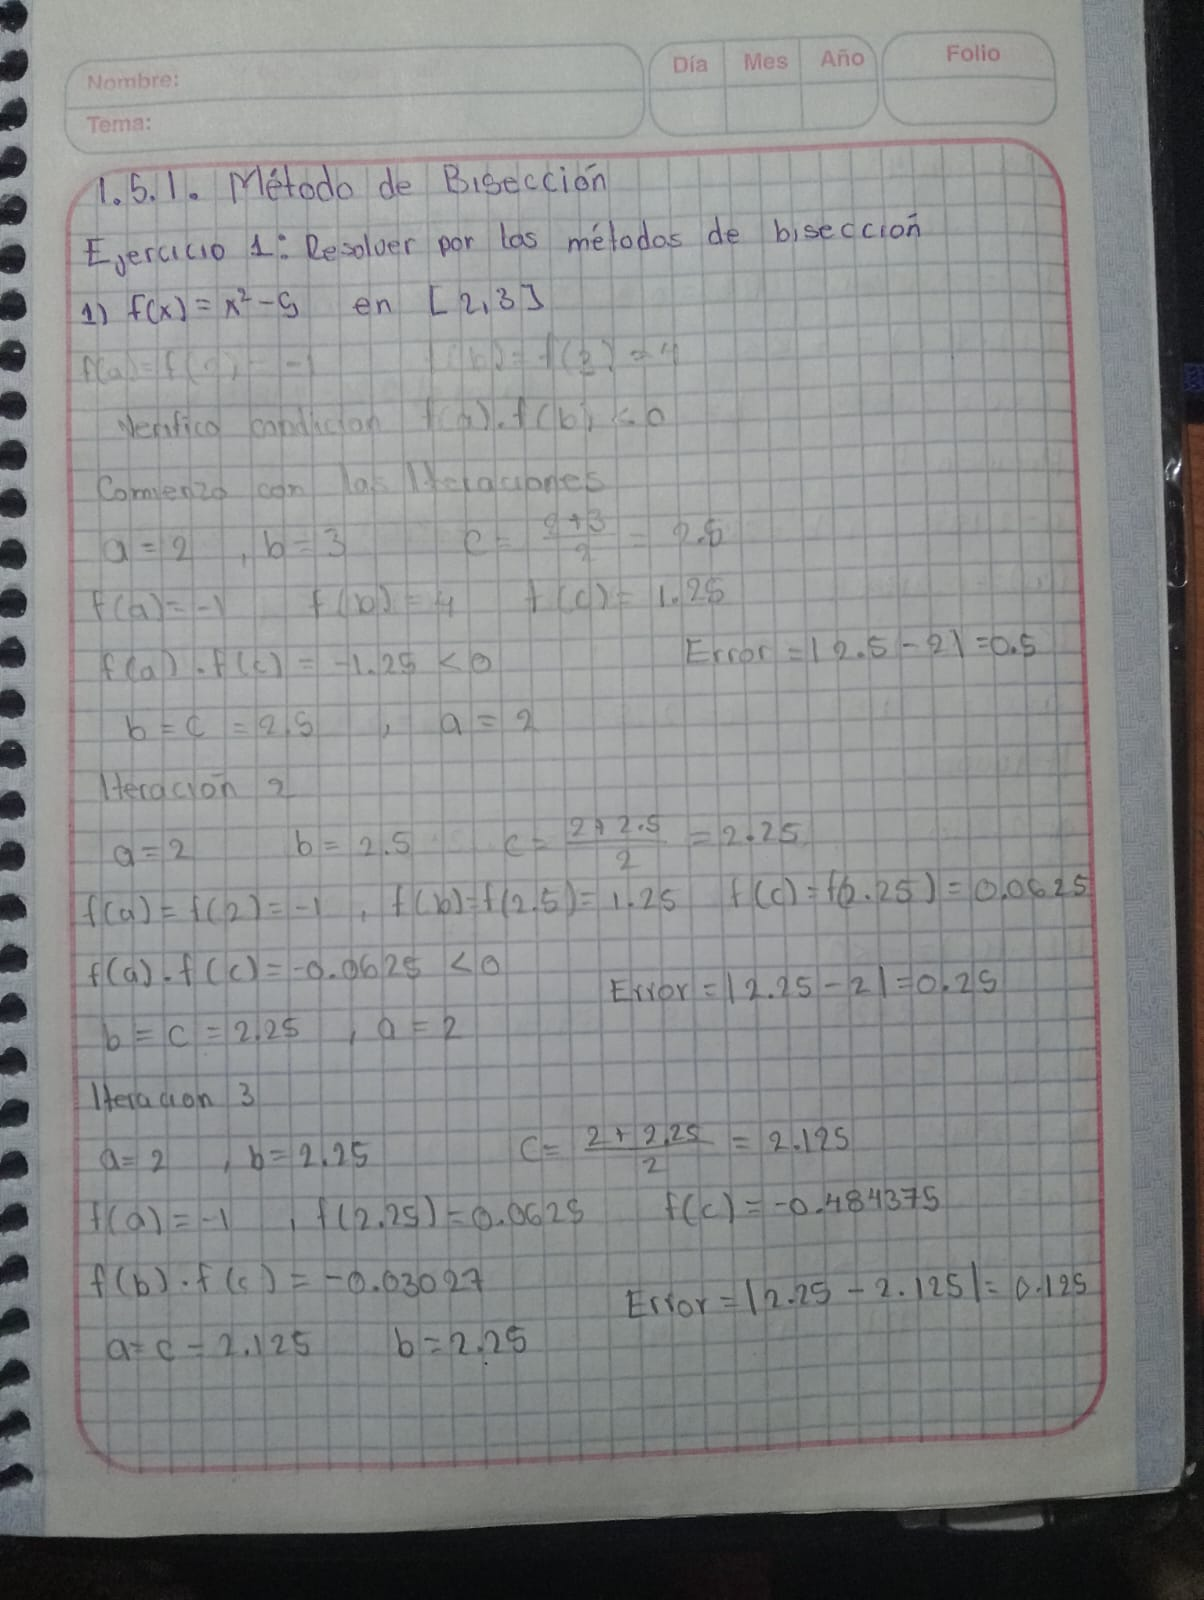
\includegraphics[width=2.60417in,height=\textheight,keepaspectratio,alt={pag.1}]{BISECCION 1.jpg}
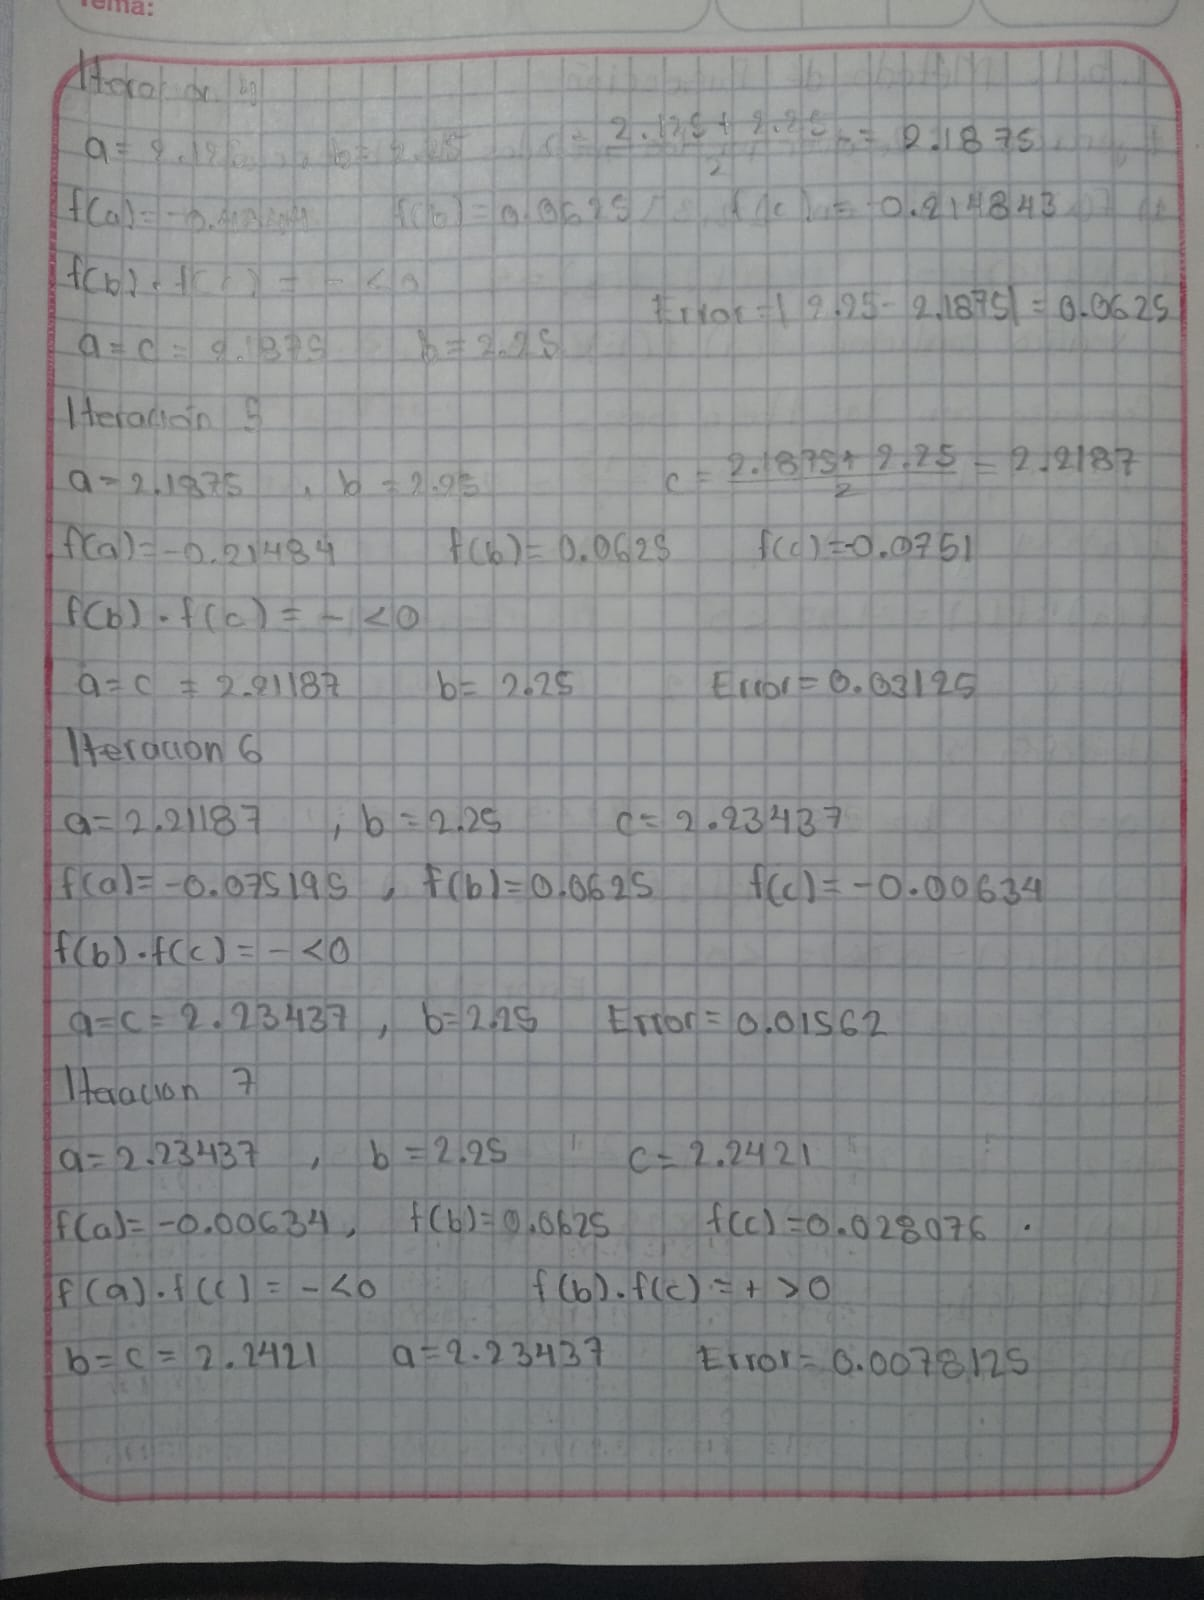
\includegraphics[width=2.60417in,height=\textheight,keepaspectratio,alt={pag.1}]{BISECCION 2.jpg}
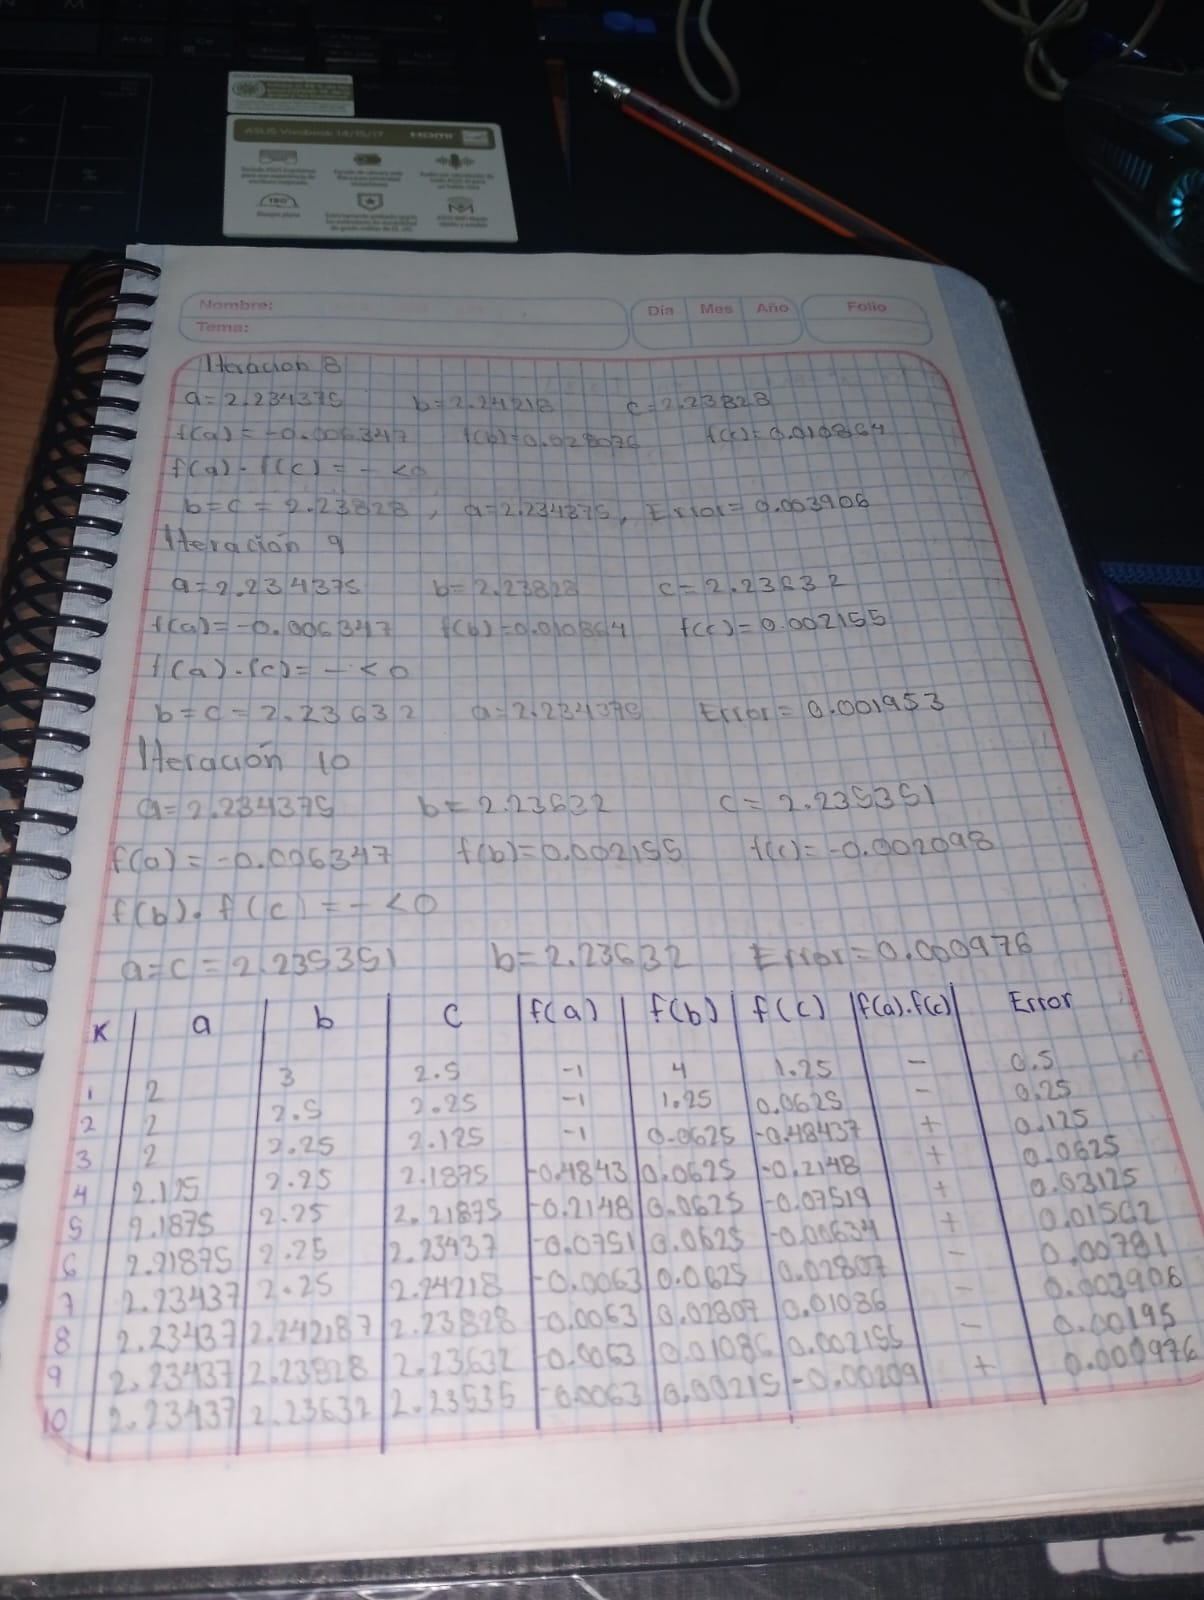
\includegraphics[width=2.60417in,height=\textheight,keepaspectratio,alt={pag.1}]{BISECCION 3.jpg}
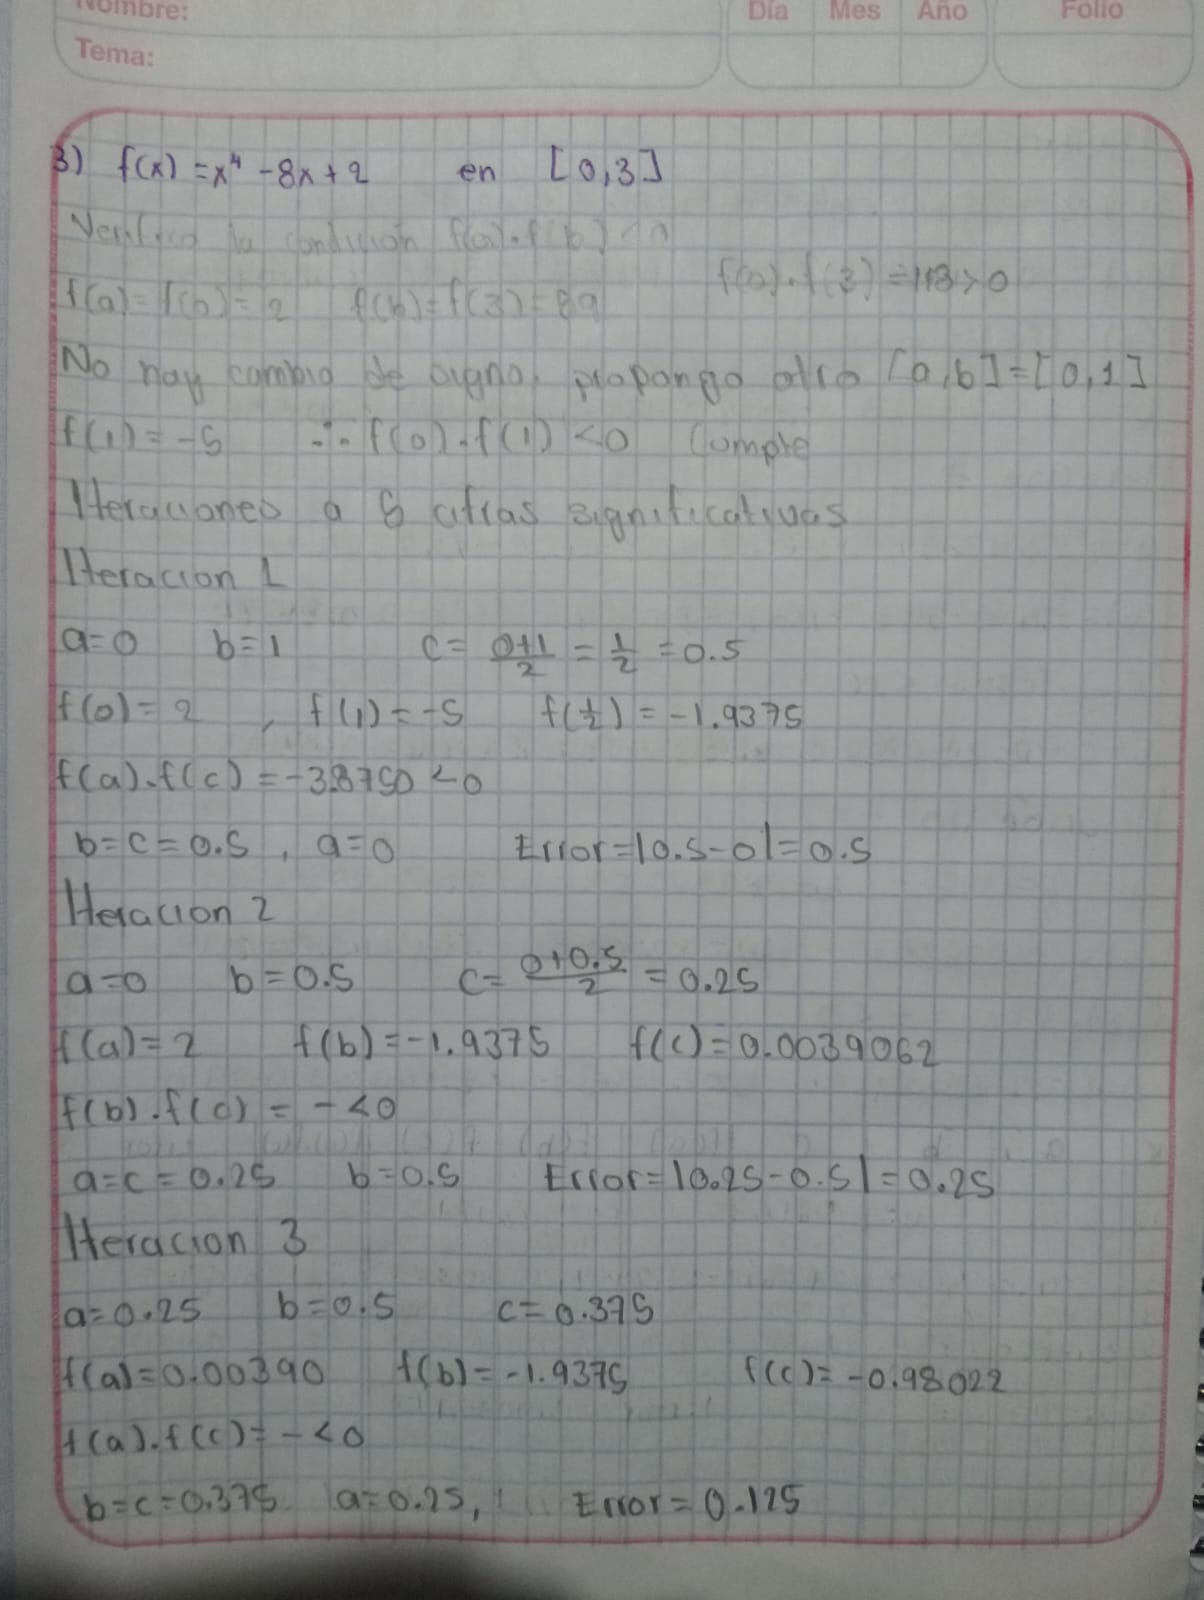
\includegraphics[width=2.60417in,height=\textheight,keepaspectratio,alt={pag.1}]{BISECCION 4.jpg}
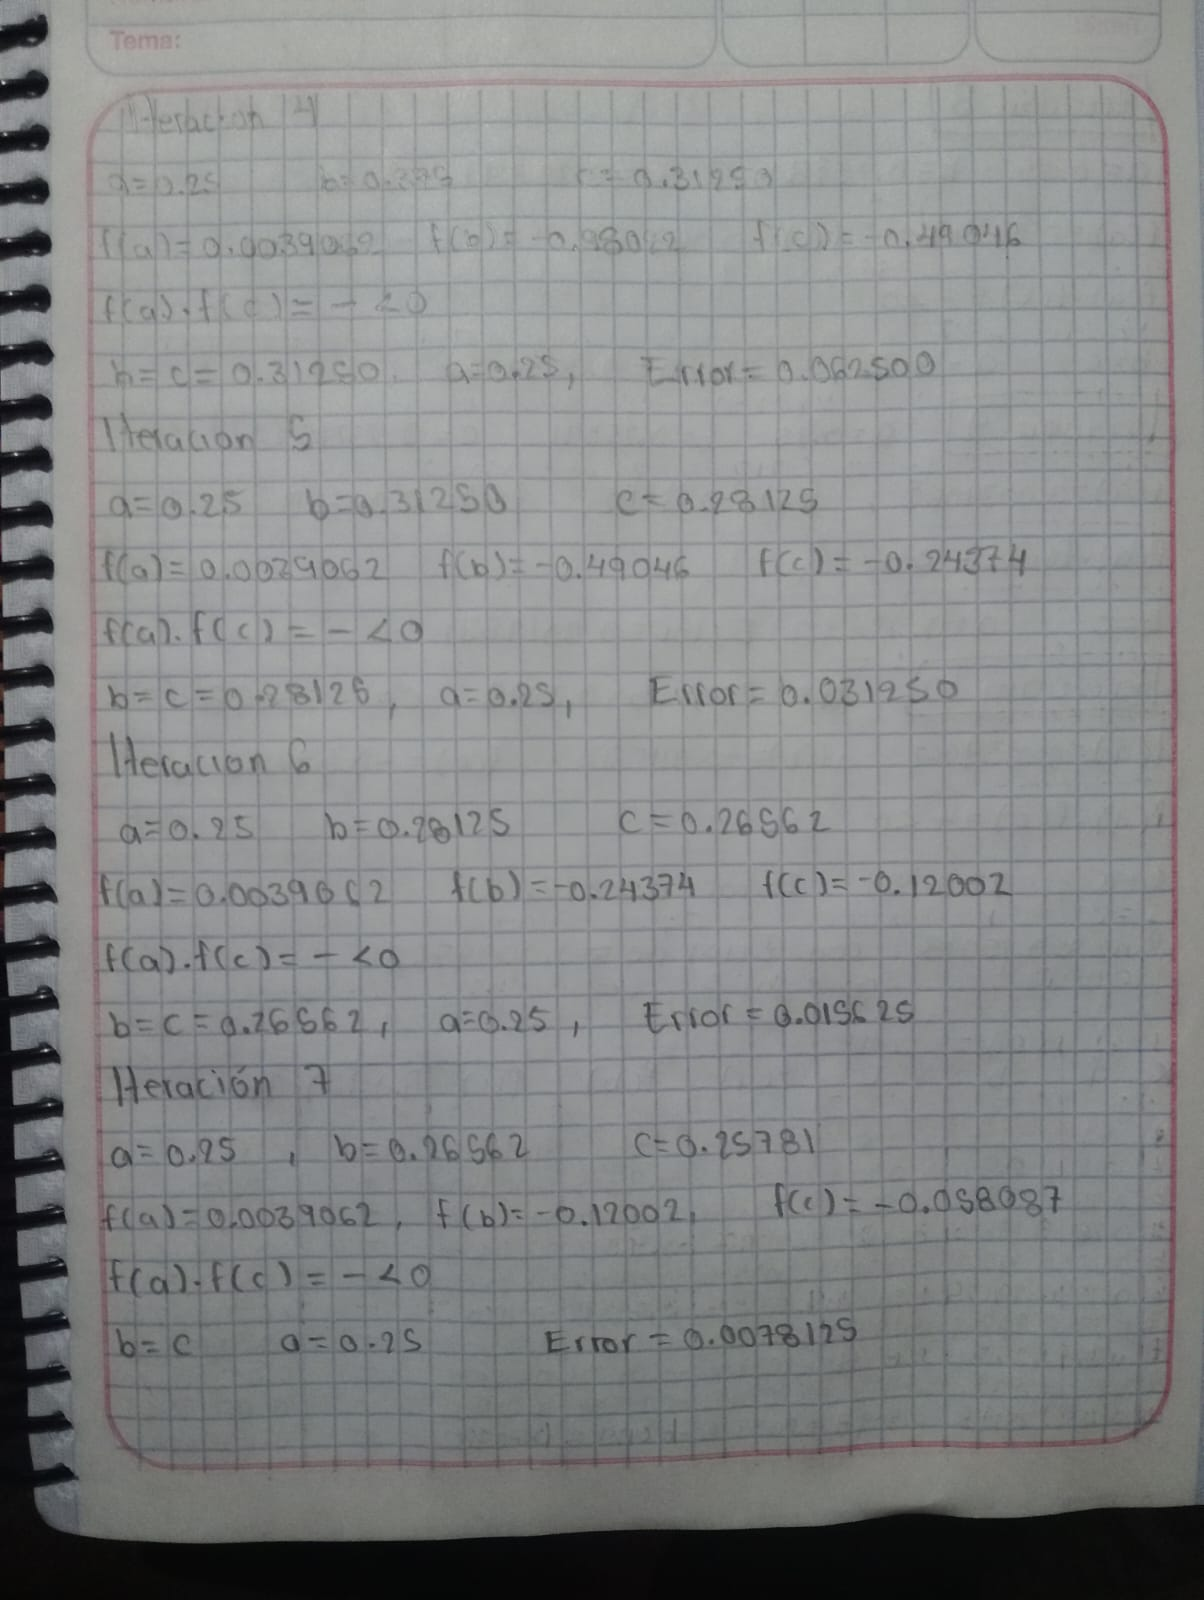
\includegraphics[width=2.60417in,height=\textheight,keepaspectratio,alt={pag.1}]{BISECCION 5.jpg}
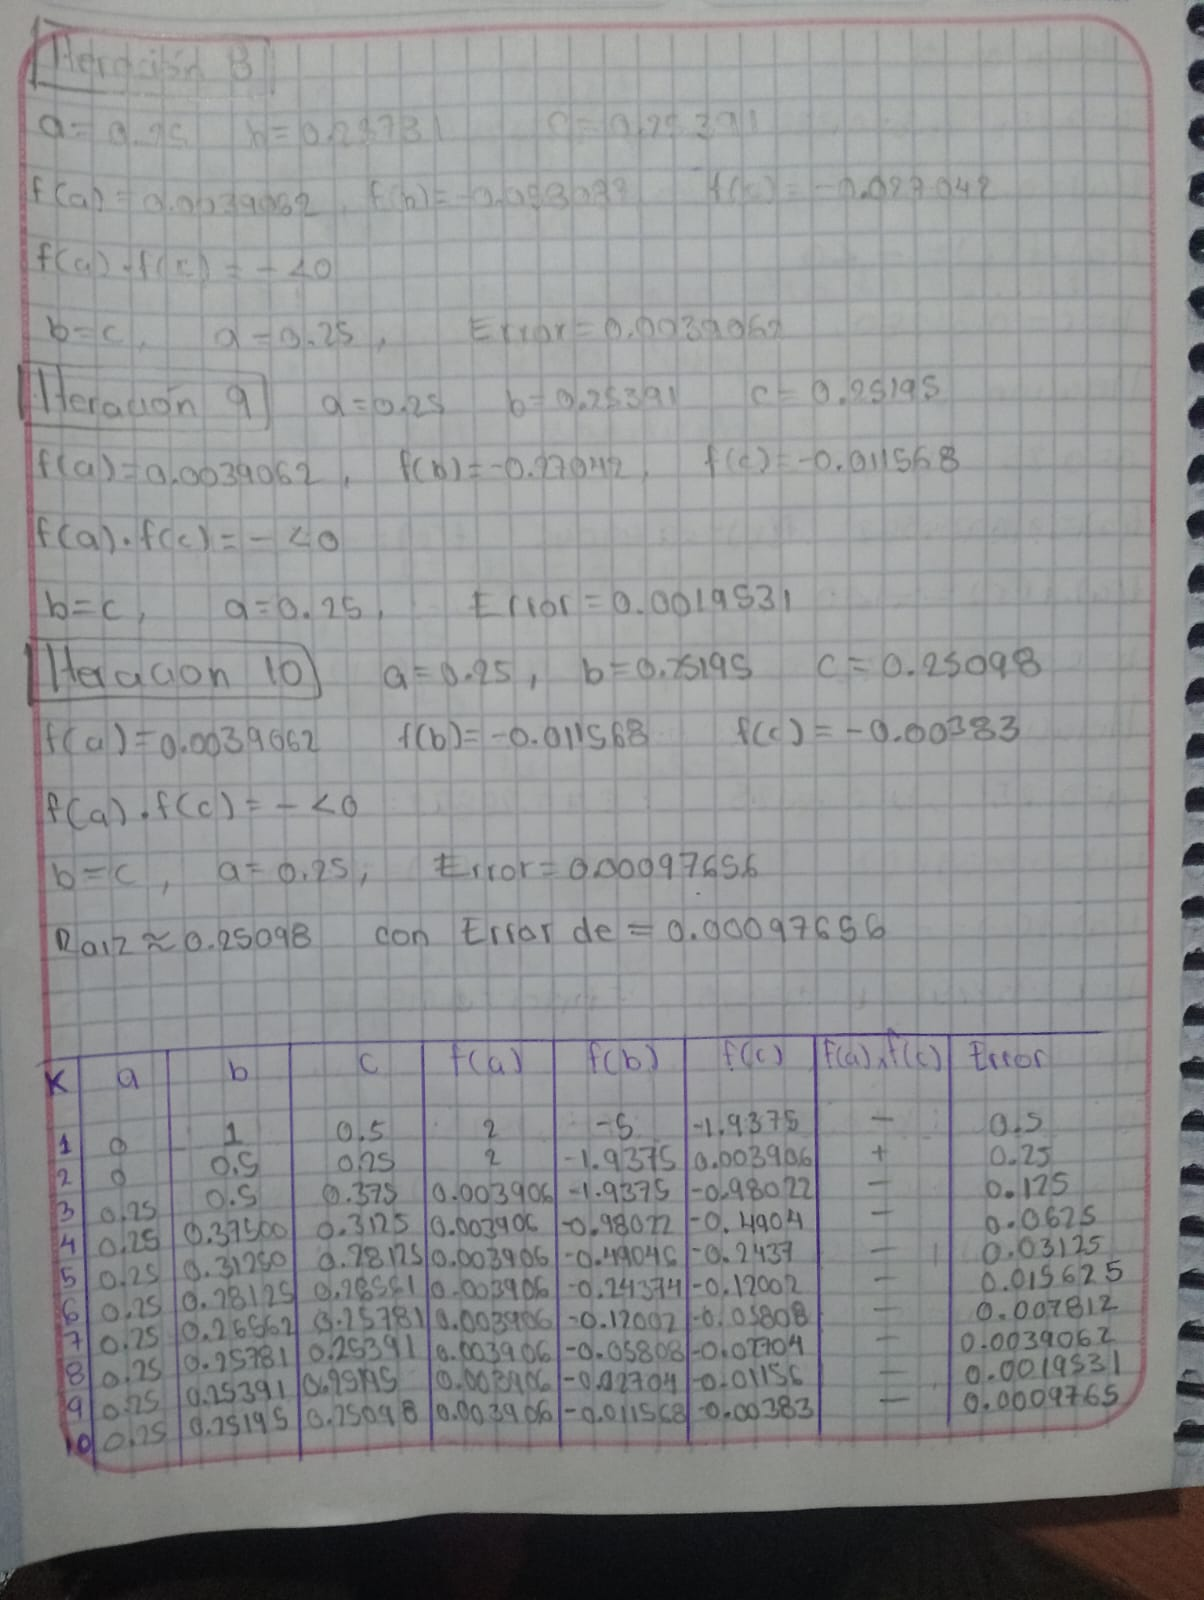
\includegraphics[width=2.60417in,height=\textheight,keepaspectratio,alt={pag.1}]{BISECCION 6.jpg}
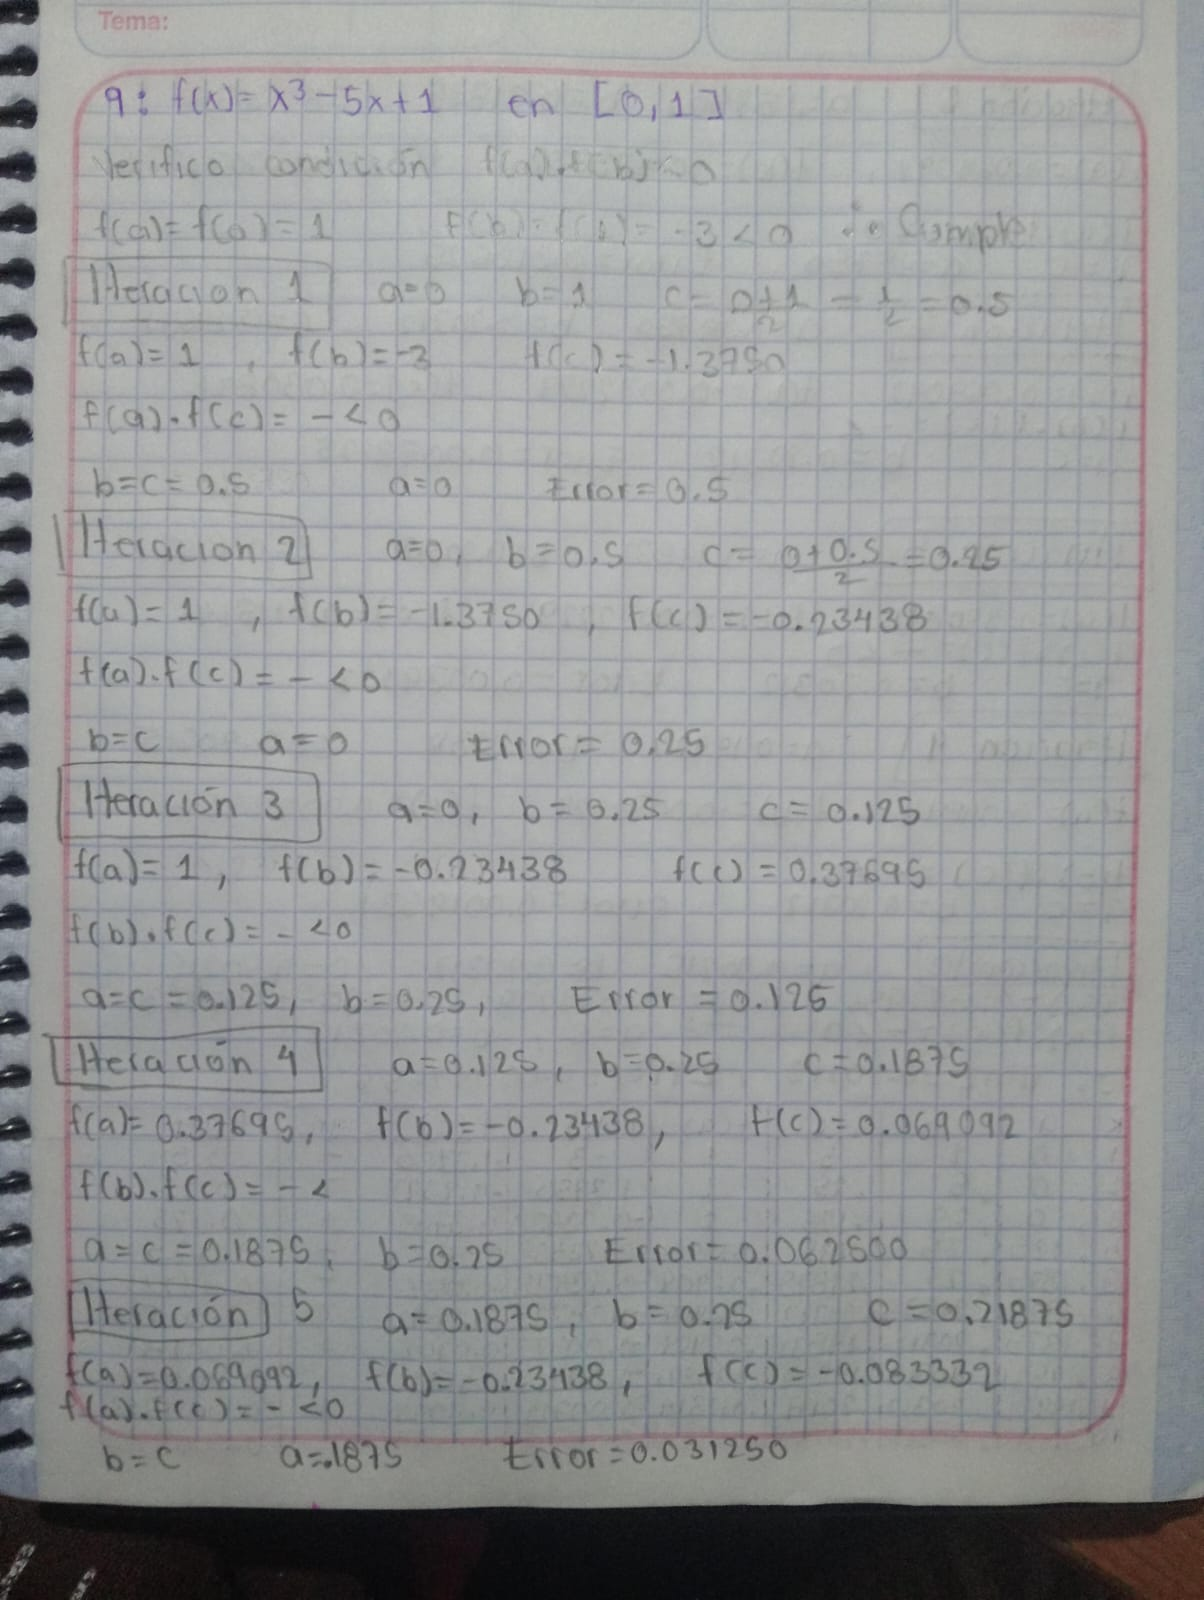
\includegraphics[width=2.60417in,height=\textheight,keepaspectratio,alt={pag.1}]{BISECCION 7.jpg}
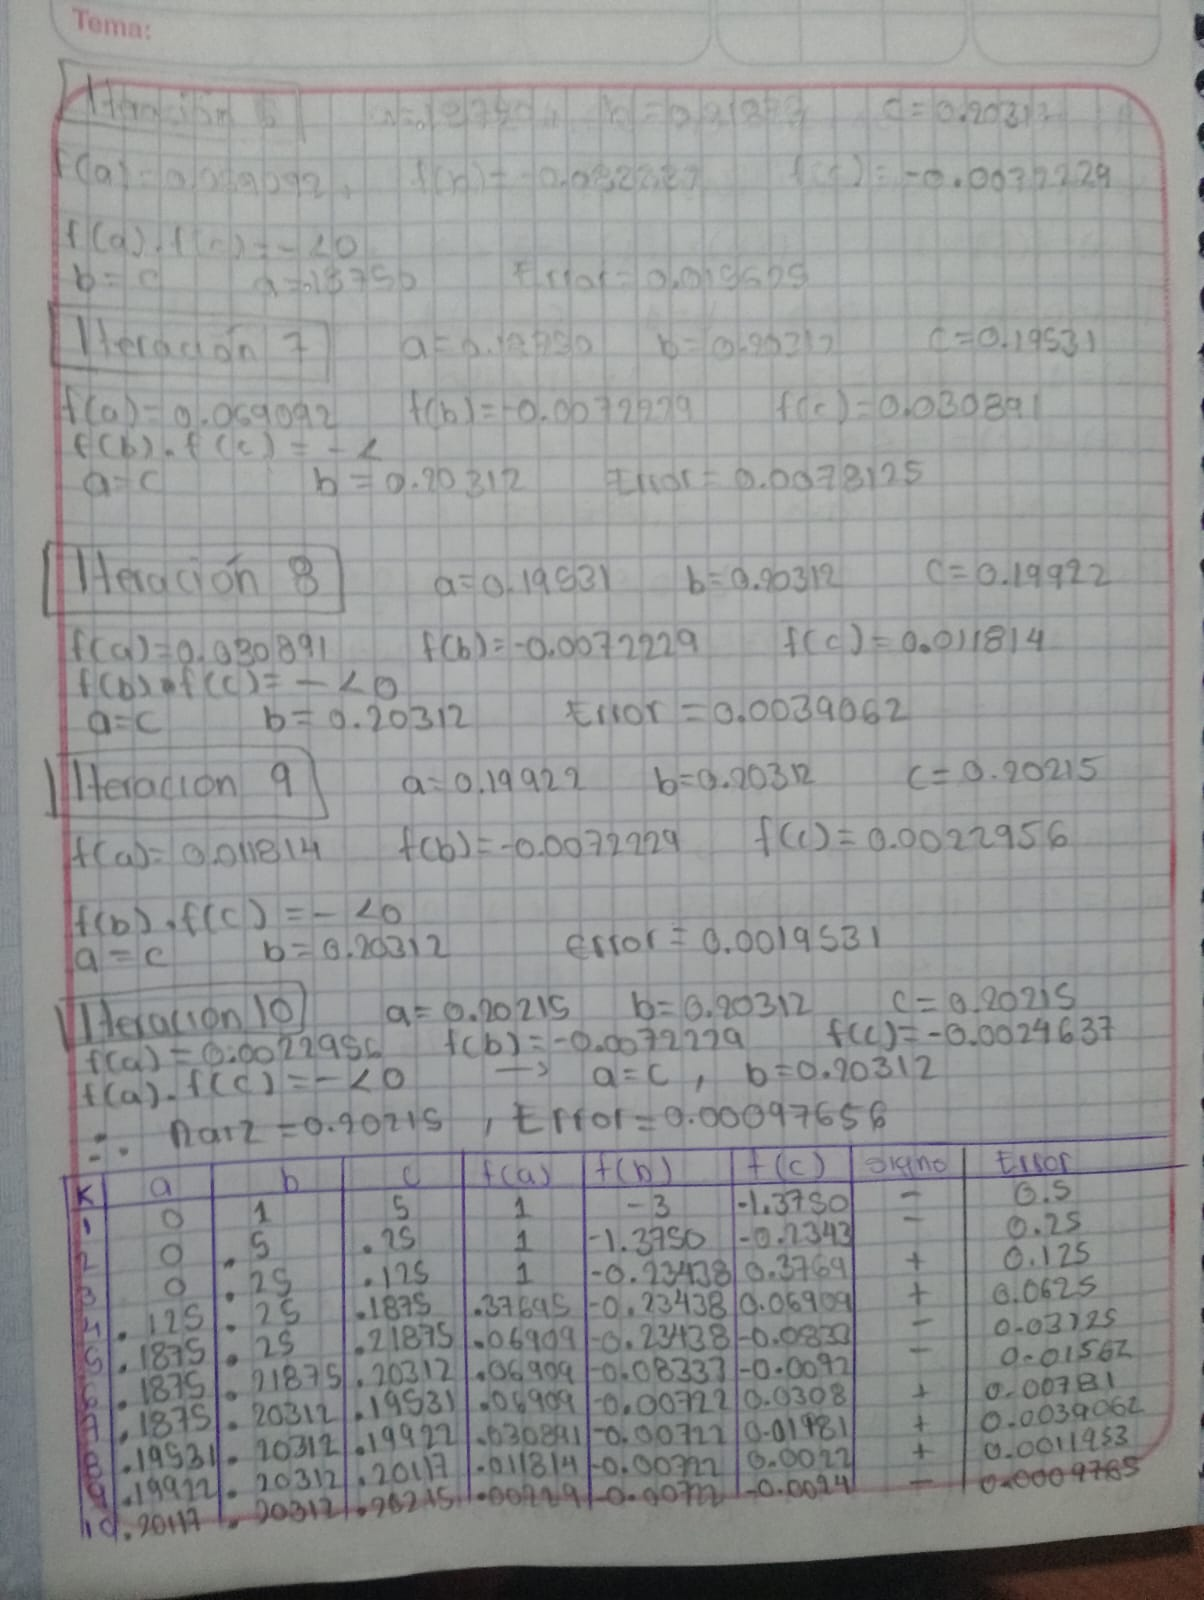
\includegraphics[width=2.60417in,height=\textheight,keepaspectratio,alt={pag.1}]{BISECCION 8.jpg}

\subsection{\texorpdfstring{\emph{Ejercicios en
código:}}{Ejercicios en código:}}\label{ejercicios-en-cuxf3digo}

\subsubsection{5:}\label{section-37}

\(f(x) = \cos(x) - x^2\) en \([0, 1]\)

\begin{Shaded}
\begin{Highlighting}[]
\NormalTok{f }\OtherTok{\textless{}{-}} \ControlFlowTok{function}\NormalTok{(x) }\FunctionTok{cos}\NormalTok{(x) }\SpecialCharTok{{-}}\NormalTok{ x}\SpecialCharTok{\^{}}\DecValTok{2}
\NormalTok{a }\OtherTok{\textless{}{-}} \FloatTok{0.0}\NormalTok{; b }\OtherTok{\textless{}{-}} \FloatTok{1.0}

\NormalTok{resultado }\OtherTok{\textless{}{-}} \FunctionTok{data.frame}\NormalTok{(}
  \AttributeTok{k =} \DecValTok{1}\SpecialCharTok{:}\DecValTok{10}\NormalTok{, }\AttributeTok{a\_k =} \FunctionTok{numeric}\NormalTok{(}\DecValTok{10}\NormalTok{), }\AttributeTok{b\_k =} \FunctionTok{numeric}\NormalTok{(}\DecValTok{10}\NormalTok{), }\AttributeTok{c\_k =} \FunctionTok{numeric}\NormalTok{(}\DecValTok{10}\NormalTok{),}
  \AttributeTok{f\_ak =} \FunctionTok{numeric}\NormalTok{(}\DecValTok{10}\NormalTok{), }\AttributeTok{f\_bk =} \FunctionTok{numeric}\NormalTok{(}\DecValTok{10}\NormalTok{), }\AttributeTok{f\_ck =} \FunctionTok{numeric}\NormalTok{(}\DecValTok{10}\NormalTok{),}
  \AttributeTok{signo =} \FunctionTok{character}\NormalTok{(}\DecValTok{10}\NormalTok{), }\AttributeTok{error =} \FunctionTok{numeric}\NormalTok{(}\DecValTok{10}\NormalTok{), }\AttributeTok{stringsAsFactors =} \ConstantTok{FALSE}
\NormalTok{)}

\NormalTok{a\_temp }\OtherTok{\textless{}{-}}\NormalTok{ a; b\_temp }\OtherTok{\textless{}{-}}\NormalTok{ b}
\ControlFlowTok{for}\NormalTok{ (k }\ControlFlowTok{in} \DecValTok{1}\SpecialCharTok{:}\DecValTok{10}\NormalTok{) \{}
\NormalTok{  c }\OtherTok{\textless{}{-}}\NormalTok{ (a\_temp }\SpecialCharTok{+}\NormalTok{ b\_temp) }\SpecialCharTok{/} \DecValTok{2}
\NormalTok{  fc }\OtherTok{\textless{}{-}} \FunctionTok{f}\NormalTok{(c)}
\NormalTok{  fak }\OtherTok{\textless{}{-}} \FunctionTok{f}\NormalTok{(a\_temp); fbk }\OtherTok{\textless{}{-}} \FunctionTok{f}\NormalTok{(b\_temp)}
\NormalTok{  error }\OtherTok{\textless{}{-}} \FunctionTok{abs}\NormalTok{(b\_temp }\SpecialCharTok{{-}}\NormalTok{ a\_temp)}
\NormalTok{  signo }\OtherTok{\textless{}{-}} \FunctionTok{ifelse}\NormalTok{(fak }\SpecialCharTok{*}\NormalTok{ fc }\SpecialCharTok{\textless{}} \DecValTok{0}\NormalTok{, }\StringTok{"{-}"}\NormalTok{, }\StringTok{"+"}\NormalTok{)}
\NormalTok{  resultado[k, }\DecValTok{2}\SpecialCharTok{:}\DecValTok{9}\NormalTok{] }\OtherTok{\textless{}{-}} \FunctionTok{list}\NormalTok{(a\_temp, b\_temp, c, fak, fbk, fc, signo, error)}
  \ControlFlowTok{if}\NormalTok{ (fak }\SpecialCharTok{*}\NormalTok{ fc }\SpecialCharTok{\textless{}} \DecValTok{0}\NormalTok{) b\_temp }\OtherTok{\textless{}{-}}\NormalTok{ c }\ControlFlowTok{else}\NormalTok{ a\_temp }\OtherTok{\textless{}{-}}\NormalTok{ c}
\NormalTok{\}}

\NormalTok{knitr}\SpecialCharTok{::}\FunctionTok{kable}\NormalTok{(resultado, }\AttributeTok{digits =} \DecValTok{6}\NormalTok{, }
             \AttributeTok{caption =} \StringTok{"10 Iteraciones para f(x) = cos(x) {-} x² en [0, 1]"}\NormalTok{)}
\end{Highlighting}
\end{Shaded}

\begin{longtable}[]{@{}
  >{\raggedleft\arraybackslash}p{(\linewidth - 16\tabcolsep) * \real{0.0405}}
  >{\raggedleft\arraybackslash}p{(\linewidth - 16\tabcolsep) * \real{0.1216}}
  >{\raggedleft\arraybackslash}p{(\linewidth - 16\tabcolsep) * \real{0.1216}}
  >{\raggedleft\arraybackslash}p{(\linewidth - 16\tabcolsep) * \real{0.1216}}
  >{\raggedleft\arraybackslash}p{(\linewidth - 16\tabcolsep) * \real{0.1216}}
  >{\raggedleft\arraybackslash}p{(\linewidth - 16\tabcolsep) * \real{0.1351}}
  >{\raggedleft\arraybackslash}p{(\linewidth - 16\tabcolsep) * \real{0.1351}}
  >{\raggedright\arraybackslash}p{(\linewidth - 16\tabcolsep) * \real{0.0811}}
  >{\raggedleft\arraybackslash}p{(\linewidth - 16\tabcolsep) * \real{0.1216}}@{}}
\caption{10 Iteraciones para f(x) = cos(x) - x² en {[}0,
1{]}}\tabularnewline
\toprule\noalign{}
\begin{minipage}[b]{\linewidth}\raggedleft
k
\end{minipage} & \begin{minipage}[b]{\linewidth}\raggedleft
a\_k
\end{minipage} & \begin{minipage}[b]{\linewidth}\raggedleft
b\_k
\end{minipage} & \begin{minipage}[b]{\linewidth}\raggedleft
c\_k
\end{minipage} & \begin{minipage}[b]{\linewidth}\raggedleft
f\_ak
\end{minipage} & \begin{minipage}[b]{\linewidth}\raggedleft
f\_bk
\end{minipage} & \begin{minipage}[b]{\linewidth}\raggedleft
f\_ck
\end{minipage} & \begin{minipage}[b]{\linewidth}\raggedright
signo
\end{minipage} & \begin{minipage}[b]{\linewidth}\raggedleft
error
\end{minipage} \\
\midrule\noalign{}
\endfirsthead
\toprule\noalign{}
\begin{minipage}[b]{\linewidth}\raggedleft
k
\end{minipage} & \begin{minipage}[b]{\linewidth}\raggedleft
a\_k
\end{minipage} & \begin{minipage}[b]{\linewidth}\raggedleft
b\_k
\end{minipage} & \begin{minipage}[b]{\linewidth}\raggedleft
c\_k
\end{minipage} & \begin{minipage}[b]{\linewidth}\raggedleft
f\_ak
\end{minipage} & \begin{minipage}[b]{\linewidth}\raggedleft
f\_bk
\end{minipage} & \begin{minipage}[b]{\linewidth}\raggedleft
f\_ck
\end{minipage} & \begin{minipage}[b]{\linewidth}\raggedright
signo
\end{minipage} & \begin{minipage}[b]{\linewidth}\raggedleft
error
\end{minipage} \\
\midrule\noalign{}
\endhead
\bottomrule\noalign{}
\endlastfoot
1 & 0.000000 & 1.000000 & 0.500000 & 1.000000 & -0.459698 & 0.627583 & +
& 1.000000 \\
2 & 0.500000 & 1.000000 & 0.750000 & 0.627583 & -0.459698 & 0.169189 & +
& 0.500000 \\
3 & 0.750000 & 1.000000 & 0.875000 & 0.169189 & -0.459698 & -0.124628 &
- & 0.250000 \\
4 & 0.750000 & 0.875000 & 0.812500 & 0.169189 & -0.124628 & 0.027529 & +
& 0.125000 \\
5 & 0.812500 & 0.875000 & 0.843750 & 0.027529 & -0.124628 & -0.047248 &
- & 0.062500 \\
6 & 0.812500 & 0.843750 & 0.828125 & 0.027529 & -0.047248 & -0.009533 &
- & 0.031250 \\
7 & 0.812500 & 0.828125 & 0.820312 & 0.027529 & -0.009533 & 0.009080 & +
& 0.015625 \\
8 & 0.820312 & 0.828125 & 0.824219 & 0.009080 & -0.009533 & -0.000206 &
- & 0.007812 \\
9 & 0.820312 & 0.824219 & 0.822266 & 0.009080 & -0.000206 & 0.004442 & +
& 0.003906 \\
10 & 0.822266 & 0.824219 & 0.823242 & 0.004442 & -0.000206 & 0.002119 &
+ & 0.001953 \\
\end{longtable}

\begin{Shaded}
\begin{Highlighting}[]
\NormalTok{x\_vals }\OtherTok{\textless{}{-}} \FunctionTok{seq}\NormalTok{(}\DecValTok{0}\NormalTok{, }\DecValTok{1}\NormalTok{, }\AttributeTok{length.out =} \DecValTok{200}\NormalTok{)}
\NormalTok{y\_vals }\OtherTok{\textless{}{-}} \FunctionTok{f}\NormalTok{(x\_vals)}

\FunctionTok{plot}\NormalTok{(x\_vals, y\_vals, }\AttributeTok{type =} \StringTok{"l"}\NormalTok{, }\AttributeTok{lwd =} \DecValTok{3}\NormalTok{, }\AttributeTok{col =} \StringTok{"blue"}\NormalTok{,}
     \AttributeTok{main =} \StringTok{"f(x) = cos(x) {-} x² en [0, 1] {-} 10 Iteraciones"}\NormalTok{,}
     \AttributeTok{xlab =} \StringTok{"x"}\NormalTok{, }\AttributeTok{ylab =} \StringTok{"f(x)"}\NormalTok{)}
\FunctionTok{abline}\NormalTok{(}\AttributeTok{h =} \DecValTok{0}\NormalTok{, }\AttributeTok{col =} \StringTok{"red"}\NormalTok{, }\AttributeTok{lty =} \DecValTok{2}\NormalTok{, }\AttributeTok{lwd =} \DecValTok{1}\NormalTok{)}

\NormalTok{colores }\OtherTok{\textless{}{-}} \FunctionTok{rainbow}\NormalTok{(}\DecValTok{10}\NormalTok{)}
\ControlFlowTok{for}\NormalTok{ (i }\ControlFlowTok{in} \DecValTok{1}\SpecialCharTok{:}\DecValTok{10}\NormalTok{) \{}
  \FunctionTok{segments}\NormalTok{(resultado}\SpecialCharTok{$}\NormalTok{a\_k[i], }\SpecialCharTok{{-}}\FloatTok{0.1}\NormalTok{, resultado}\SpecialCharTok{$}\NormalTok{b\_k[i], }\SpecialCharTok{{-}}\FloatTok{0.1}\NormalTok{, }
           \AttributeTok{col =}\NormalTok{ colores[i], }\AttributeTok{lwd =} \DecValTok{3}\NormalTok{)}
  \FunctionTok{points}\NormalTok{(resultado}\SpecialCharTok{$}\NormalTok{c\_k[i], }\DecValTok{0}\NormalTok{, }\AttributeTok{col =}\NormalTok{ colores[i], }\AttributeTok{pch =} \DecValTok{19}\NormalTok{, }\AttributeTok{cex =} \FloatTok{1.2}\NormalTok{)}
  \ControlFlowTok{if}\NormalTok{(i }\SpecialCharTok{\%\%} \DecValTok{2} \SpecialCharTok{==} \DecValTok{0}\NormalTok{) \{}
    \FunctionTok{text}\NormalTok{(resultado}\SpecialCharTok{$}\NormalTok{c\_k[i], }\FloatTok{0.1}\NormalTok{, }\AttributeTok{labels =}\NormalTok{ i, }\AttributeTok{col =}\NormalTok{ colores[i], }\AttributeTok{font =} \DecValTok{2}\NormalTok{, }\AttributeTok{cex =} \FloatTok{0.8}\NormalTok{)}
\NormalTok{  \}}
\NormalTok{\}}

\FunctionTok{legend}\NormalTok{(}\StringTok{"topright"}\NormalTok{, }
       \AttributeTok{legend =} \FunctionTok{c}\NormalTok{(}\StringTok{"f(x)"}\NormalTok{, }\StringTok{"Eje x"}\NormalTok{, }\StringTok{"Intervalos"}\NormalTok{, }\StringTok{"Puntos c\_k"}\NormalTok{),}
       \AttributeTok{col =} \FunctionTok{c}\NormalTok{(}\StringTok{"blue"}\NormalTok{, }\StringTok{"red"}\NormalTok{, }\StringTok{"purple"}\NormalTok{, }\StringTok{"green"}\NormalTok{),}
       \AttributeTok{lty =} \FunctionTok{c}\NormalTok{(}\DecValTok{1}\NormalTok{, }\DecValTok{2}\NormalTok{, }\DecValTok{1}\NormalTok{, }\ConstantTok{NA}\NormalTok{), }\AttributeTok{pch =} \FunctionTok{c}\NormalTok{(}\ConstantTok{NA}\NormalTok{, }\ConstantTok{NA}\NormalTok{, }\ConstantTok{NA}\NormalTok{, }\DecValTok{19}\NormalTok{),}
       \AttributeTok{lwd =} \FunctionTok{c}\NormalTok{(}\DecValTok{3}\NormalTok{, }\DecValTok{1}\NormalTok{, }\DecValTok{3}\NormalTok{, }\ConstantTok{NA}\NormalTok{))}
\end{Highlighting}
\end{Shaded}

\pandocbounded{\includegraphics[keepaspectratio]{Notas_MN_LILIANA_CS_files/figure-latex/unnamed-chunk-444-1.pdf}}

\subsubsection{7:}\label{section-38}

\(f(x) = -4x^2 + 5x + 6\) en \([-1, 0]\)

\begin{Shaded}
\begin{Highlighting}[]
\NormalTok{f }\OtherTok{\textless{}{-}} \ControlFlowTok{function}\NormalTok{(x) }\SpecialCharTok{{-}}\DecValTok{4}\SpecialCharTok{*}\NormalTok{x}\SpecialCharTok{\^{}}\DecValTok{2} \SpecialCharTok{+} \DecValTok{5}\SpecialCharTok{*}\NormalTok{x }\SpecialCharTok{+} \DecValTok{6}
\NormalTok{a }\OtherTok{\textless{}{-}} \SpecialCharTok{{-}}\FloatTok{1.0}\NormalTok{; b }\OtherTok{\textless{}{-}} \FloatTok{0.0}

\NormalTok{resultado }\OtherTok{\textless{}{-}} \FunctionTok{data.frame}\NormalTok{(}
  \AttributeTok{k =} \DecValTok{1}\SpecialCharTok{:}\DecValTok{10}\NormalTok{, }\AttributeTok{a\_k =} \FunctionTok{numeric}\NormalTok{(}\DecValTok{10}\NormalTok{), }\AttributeTok{b\_k =} \FunctionTok{numeric}\NormalTok{(}\DecValTok{10}\NormalTok{), }\AttributeTok{c\_k =} \FunctionTok{numeric}\NormalTok{(}\DecValTok{10}\NormalTok{),}
  \AttributeTok{f\_ak =} \FunctionTok{numeric}\NormalTok{(}\DecValTok{10}\NormalTok{), }\AttributeTok{f\_bk =} \FunctionTok{numeric}\NormalTok{(}\DecValTok{10}\NormalTok{), }\AttributeTok{f\_ck =} \FunctionTok{numeric}\NormalTok{(}\DecValTok{10}\NormalTok{),}
  \AttributeTok{signo =} \FunctionTok{character}\NormalTok{(}\DecValTok{10}\NormalTok{), }\AttributeTok{error =} \FunctionTok{numeric}\NormalTok{(}\DecValTok{10}\NormalTok{), }\AttributeTok{stringsAsFactors =} \ConstantTok{FALSE}
\NormalTok{)}

\NormalTok{a\_temp }\OtherTok{\textless{}{-}}\NormalTok{ a; b\_temp }\OtherTok{\textless{}{-}}\NormalTok{ b}
\ControlFlowTok{for}\NormalTok{ (k }\ControlFlowTok{in} \DecValTok{1}\SpecialCharTok{:}\DecValTok{10}\NormalTok{) \{}
\NormalTok{  c }\OtherTok{\textless{}{-}}\NormalTok{ (a\_temp }\SpecialCharTok{+}\NormalTok{ b\_temp) }\SpecialCharTok{/} \DecValTok{2}
\NormalTok{  fc }\OtherTok{\textless{}{-}} \FunctionTok{f}\NormalTok{(c)}
\NormalTok{  fak }\OtherTok{\textless{}{-}} \FunctionTok{f}\NormalTok{(a\_temp); fbk }\OtherTok{\textless{}{-}} \FunctionTok{f}\NormalTok{(b\_temp)}
\NormalTok{  error }\OtherTok{\textless{}{-}} \FunctionTok{abs}\NormalTok{(b\_temp }\SpecialCharTok{{-}}\NormalTok{ a\_temp)}
\NormalTok{  signo }\OtherTok{\textless{}{-}} \FunctionTok{ifelse}\NormalTok{(fak }\SpecialCharTok{*}\NormalTok{ fc }\SpecialCharTok{\textless{}} \DecValTok{0}\NormalTok{, }\StringTok{"{-}"}\NormalTok{, }\StringTok{"+"}\NormalTok{)}
\NormalTok{  resultado[k, }\DecValTok{2}\SpecialCharTok{:}\DecValTok{9}\NormalTok{] }\OtherTok{\textless{}{-}} \FunctionTok{list}\NormalTok{(a\_temp, b\_temp, c, fak, fbk, fc, signo, error)}
  \ControlFlowTok{if}\NormalTok{ (fak }\SpecialCharTok{*}\NormalTok{ fc }\SpecialCharTok{\textless{}} \DecValTok{0}\NormalTok{) b\_temp }\OtherTok{\textless{}{-}}\NormalTok{ c }\ControlFlowTok{else}\NormalTok{ a\_temp }\OtherTok{\textless{}{-}}\NormalTok{ c}
\NormalTok{\}}

\NormalTok{knitr}\SpecialCharTok{::}\FunctionTok{kable}\NormalTok{(resultado, }\AttributeTok{digits =} \DecValTok{6}\NormalTok{, }
             \AttributeTok{caption =} \StringTok{"10 Iteraciones para f(x) = {-}4x² + 5x + 6 en [{-}1, 0]"}\NormalTok{)}
\end{Highlighting}
\end{Shaded}

\begin{longtable}[]{@{}
  >{\raggedleft\arraybackslash}p{(\linewidth - 16\tabcolsep) * \real{0.0448}}
  >{\raggedleft\arraybackslash}p{(\linewidth - 16\tabcolsep) * \real{0.1493}}
  >{\raggedleft\arraybackslash}p{(\linewidth - 16\tabcolsep) * \real{0.0746}}
  >{\raggedleft\arraybackslash}p{(\linewidth - 16\tabcolsep) * \real{0.1493}}
  >{\raggedleft\arraybackslash}p{(\linewidth - 16\tabcolsep) * \real{0.1493}}
  >{\raggedleft\arraybackslash}p{(\linewidth - 16\tabcolsep) * \real{0.0746}}
  >{\raggedleft\arraybackslash}p{(\linewidth - 16\tabcolsep) * \real{0.1343}}
  >{\raggedright\arraybackslash}p{(\linewidth - 16\tabcolsep) * \real{0.0896}}
  >{\raggedleft\arraybackslash}p{(\linewidth - 16\tabcolsep) * \real{0.1343}}@{}}
\caption{10 Iteraciones para f(x) = -4x² + 5x + 6 en {[}-1,
0{]}}\tabularnewline
\toprule\noalign{}
\begin{minipage}[b]{\linewidth}\raggedleft
k
\end{minipage} & \begin{minipage}[b]{\linewidth}\raggedleft
a\_k
\end{minipage} & \begin{minipage}[b]{\linewidth}\raggedleft
b\_k
\end{minipage} & \begin{minipage}[b]{\linewidth}\raggedleft
c\_k
\end{minipage} & \begin{minipage}[b]{\linewidth}\raggedleft
f\_ak
\end{minipage} & \begin{minipage}[b]{\linewidth}\raggedleft
f\_bk
\end{minipage} & \begin{minipage}[b]{\linewidth}\raggedleft
f\_ck
\end{minipage} & \begin{minipage}[b]{\linewidth}\raggedright
signo
\end{minipage} & \begin{minipage}[b]{\linewidth}\raggedleft
error
\end{minipage} \\
\midrule\noalign{}
\endfirsthead
\toprule\noalign{}
\begin{minipage}[b]{\linewidth}\raggedleft
k
\end{minipage} & \begin{minipage}[b]{\linewidth}\raggedleft
a\_k
\end{minipage} & \begin{minipage}[b]{\linewidth}\raggedleft
b\_k
\end{minipage} & \begin{minipage}[b]{\linewidth}\raggedleft
c\_k
\end{minipage} & \begin{minipage}[b]{\linewidth}\raggedleft
f\_ak
\end{minipage} & \begin{minipage}[b]{\linewidth}\raggedleft
f\_bk
\end{minipage} & \begin{minipage}[b]{\linewidth}\raggedleft
f\_ck
\end{minipage} & \begin{minipage}[b]{\linewidth}\raggedright
signo
\end{minipage} & \begin{minipage}[b]{\linewidth}\raggedleft
error
\end{minipage} \\
\midrule\noalign{}
\endhead
\bottomrule\noalign{}
\endlastfoot
1 & -1.000000 & 0.0 & -0.500000 & -3.000000 & 6.0 & 2.500000 & - &
1.000000 \\
2 & -1.000000 & -0.5 & -0.750000 & -3.000000 & 2.5 & 0.000000 & + &
0.500000 \\
3 & -0.750000 & -0.5 & -0.625000 & 0.000000 & 2.5 & 1.312500 & + &
0.250000 \\
4 & -0.625000 & -0.5 & -0.562500 & 1.312500 & 2.5 & 1.921875 & + &
0.125000 \\
5 & -0.562500 & -0.5 & -0.531250 & 1.921875 & 2.5 & 2.214844 & + &
0.062500 \\
6 & -0.531250 & -0.5 & -0.515625 & 2.214844 & 2.5 & 2.358398 & + &
0.031250 \\
7 & -0.515625 & -0.5 & -0.507812 & 2.358398 & 2.5 & 2.429443 & + &
0.015625 \\
8 & -0.507812 & -0.5 & -0.503906 & 2.429443 & 2.5 & 2.464783 & + &
0.007812 \\
9 & -0.503906 & -0.5 & -0.501953 & 2.464783 & 2.5 & 2.482407 & + &
0.003906 \\
10 & -0.501953 & -0.5 & -0.500977 & 2.482407 & 2.5 & 2.491207 & + &
0.001953 \\
\end{longtable}

\begin{Shaded}
\begin{Highlighting}[]
\NormalTok{x\_vals }\OtherTok{\textless{}{-}} \FunctionTok{seq}\NormalTok{(}\SpecialCharTok{{-}}\DecValTok{1}\NormalTok{, }\DecValTok{0}\NormalTok{, }\AttributeTok{length.out =} \DecValTok{200}\NormalTok{)}
\NormalTok{y\_vals }\OtherTok{\textless{}{-}} \FunctionTok{f}\NormalTok{(x\_vals)}

\FunctionTok{plot}\NormalTok{(x\_vals, y\_vals, }\AttributeTok{type =} \StringTok{"l"}\NormalTok{, }\AttributeTok{lwd =} \DecValTok{3}\NormalTok{, }\AttributeTok{col =} \StringTok{"blue"}\NormalTok{,}
     \AttributeTok{main =} \StringTok{"f(x) = {-}4x² + 5x + 6 en [{-}1, 0] {-} 10 Iteraciones"}\NormalTok{,}
     \AttributeTok{xlab =} \StringTok{"x"}\NormalTok{, }\AttributeTok{ylab =} \StringTok{"f(x)"}\NormalTok{)}
\FunctionTok{abline}\NormalTok{(}\AttributeTok{h =} \DecValTok{0}\NormalTok{, }\AttributeTok{col =} \StringTok{"red"}\NormalTok{, }\AttributeTok{lty =} \DecValTok{2}\NormalTok{, }\AttributeTok{lwd =} \DecValTok{1}\NormalTok{)}

\NormalTok{colores }\OtherTok{\textless{}{-}} \FunctionTok{rainbow}\NormalTok{(}\DecValTok{10}\NormalTok{)}
\ControlFlowTok{for}\NormalTok{ (i }\ControlFlowTok{in} \DecValTok{1}\SpecialCharTok{:}\DecValTok{10}\NormalTok{) \{}
  \FunctionTok{segments}\NormalTok{(resultado}\SpecialCharTok{$}\NormalTok{a\_k[i], }\SpecialCharTok{{-}}\FloatTok{0.5}\NormalTok{, resultado}\SpecialCharTok{$}\NormalTok{b\_k[i], }\SpecialCharTok{{-}}\FloatTok{0.5}\NormalTok{, }
           \AttributeTok{col =}\NormalTok{ colores[i], }\AttributeTok{lwd =} \DecValTok{3}\NormalTok{)}
  \FunctionTok{points}\NormalTok{(resultado}\SpecialCharTok{$}\NormalTok{c\_k[i], }\DecValTok{0}\NormalTok{, }\AttributeTok{col =}\NormalTok{ colores[i], }\AttributeTok{pch =} \DecValTok{19}\NormalTok{, }\AttributeTok{cex =} \FloatTok{1.2}\NormalTok{)}
  \ControlFlowTok{if}\NormalTok{(i }\SpecialCharTok{\%\%} \DecValTok{2} \SpecialCharTok{==} \DecValTok{0}\NormalTok{) \{}
    \FunctionTok{text}\NormalTok{(resultado}\SpecialCharTok{$}\NormalTok{c\_k[i], }\FloatTok{0.5}\NormalTok{, }\AttributeTok{labels =}\NormalTok{ i, }\AttributeTok{col =}\NormalTok{ colores[i], }\AttributeTok{font =} \DecValTok{2}\NormalTok{, }\AttributeTok{cex =} \FloatTok{0.8}\NormalTok{)}
\NormalTok{  \}}
\NormalTok{\}}

\FunctionTok{legend}\NormalTok{(}\StringTok{"topleft"}\NormalTok{, }
       \AttributeTok{legend =} \FunctionTok{c}\NormalTok{(}\StringTok{"f(x)"}\NormalTok{, }\StringTok{"Eje x"}\NormalTok{, }\StringTok{"Intervalos"}\NormalTok{, }\StringTok{"Puntos c\_k"}\NormalTok{),}
       \AttributeTok{col =} \FunctionTok{c}\NormalTok{(}\StringTok{"blue"}\NormalTok{, }\StringTok{"red"}\NormalTok{, }\StringTok{"purple"}\NormalTok{, }\StringTok{"green"}\NormalTok{),}
       \AttributeTok{lty =} \FunctionTok{c}\NormalTok{(}\DecValTok{1}\NormalTok{, }\DecValTok{2}\NormalTok{, }\DecValTok{1}\NormalTok{, }\ConstantTok{NA}\NormalTok{), }\AttributeTok{pch =} \FunctionTok{c}\NormalTok{(}\ConstantTok{NA}\NormalTok{, }\ConstantTok{NA}\NormalTok{, }\ConstantTok{NA}\NormalTok{, }\DecValTok{19}\NormalTok{),}
       \AttributeTok{lwd =} \FunctionTok{c}\NormalTok{(}\DecValTok{3}\NormalTok{, }\DecValTok{1}\NormalTok{, }\DecValTok{3}\NormalTok{, }\ConstantTok{NA}\NormalTok{))}
\end{Highlighting}
\end{Shaded}

\pandocbounded{\includegraphics[keepaspectratio]{Notas_MN_LILIANA_CS_files/figure-latex/unnamed-chunk-446-1.pdf}}

\subsubsection{11:}\label{section-39}

\(f(x) = -2x^4 + 4x^3 + 6x^2 - 3x + 2\) en \([-2, -1]\)

\begin{Shaded}
\begin{Highlighting}[]
\NormalTok{f }\OtherTok{\textless{}{-}} \ControlFlowTok{function}\NormalTok{(x) }\SpecialCharTok{{-}}\DecValTok{2}\SpecialCharTok{*}\NormalTok{x}\SpecialCharTok{\^{}}\DecValTok{4} \SpecialCharTok{+} \DecValTok{4}\SpecialCharTok{*}\NormalTok{x}\SpecialCharTok{\^{}}\DecValTok{3} \SpecialCharTok{+} \DecValTok{6}\SpecialCharTok{*}\NormalTok{x}\SpecialCharTok{\^{}}\DecValTok{2} \SpecialCharTok{{-}} \DecValTok{3}\SpecialCharTok{*}\NormalTok{x }\SpecialCharTok{+} \DecValTok{2}
\NormalTok{a }\OtherTok{\textless{}{-}} \SpecialCharTok{{-}}\FloatTok{2.0}\NormalTok{; b }\OtherTok{\textless{}{-}} \SpecialCharTok{{-}}\FloatTok{1.0}

\NormalTok{resultado }\OtherTok{\textless{}{-}} \FunctionTok{data.frame}\NormalTok{(}
  \AttributeTok{k =} \DecValTok{1}\SpecialCharTok{:}\DecValTok{10}\NormalTok{, }\AttributeTok{a\_k =} \FunctionTok{numeric}\NormalTok{(}\DecValTok{10}\NormalTok{), }\AttributeTok{b\_k =} \FunctionTok{numeric}\NormalTok{(}\DecValTok{10}\NormalTok{), }\AttributeTok{c\_k =} \FunctionTok{numeric}\NormalTok{(}\DecValTok{10}\NormalTok{),}
  \AttributeTok{f\_ak =} \FunctionTok{numeric}\NormalTok{(}\DecValTok{10}\NormalTok{), }\AttributeTok{f\_bk =} \FunctionTok{numeric}\NormalTok{(}\DecValTok{10}\NormalTok{), }\AttributeTok{f\_ck =} \FunctionTok{numeric}\NormalTok{(}\DecValTok{10}\NormalTok{),}
  \AttributeTok{signo =} \FunctionTok{character}\NormalTok{(}\DecValTok{10}\NormalTok{), }\AttributeTok{error =} \FunctionTok{numeric}\NormalTok{(}\DecValTok{10}\NormalTok{), }\AttributeTok{stringsAsFactors =} \ConstantTok{FALSE}
\NormalTok{)}

\NormalTok{a\_temp }\OtherTok{\textless{}{-}}\NormalTok{ a; b\_temp }\OtherTok{\textless{}{-}}\NormalTok{ b}
\ControlFlowTok{for}\NormalTok{ (k }\ControlFlowTok{in} \DecValTok{1}\SpecialCharTok{:}\DecValTok{10}\NormalTok{) \{}
\NormalTok{  c }\OtherTok{\textless{}{-}}\NormalTok{ (a\_temp }\SpecialCharTok{+}\NormalTok{ b\_temp) }\SpecialCharTok{/} \DecValTok{2}
\NormalTok{  fc }\OtherTok{\textless{}{-}} \FunctionTok{f}\NormalTok{(c)}
\NormalTok{  fak }\OtherTok{\textless{}{-}} \FunctionTok{f}\NormalTok{(a\_temp); fbk }\OtherTok{\textless{}{-}} \FunctionTok{f}\NormalTok{(b\_temp)}
\NormalTok{  error }\OtherTok{\textless{}{-}} \FunctionTok{abs}\NormalTok{(b\_temp }\SpecialCharTok{{-}}\NormalTok{ a\_temp)}
\NormalTok{  signo }\OtherTok{\textless{}{-}} \FunctionTok{ifelse}\NormalTok{(fak }\SpecialCharTok{*}\NormalTok{ fc }\SpecialCharTok{\textless{}} \DecValTok{0}\NormalTok{, }\StringTok{"{-}"}\NormalTok{, }\StringTok{"+"}\NormalTok{)}
\NormalTok{  resultado[k, }\DecValTok{2}\SpecialCharTok{:}\DecValTok{9}\NormalTok{] }\OtherTok{\textless{}{-}} \FunctionTok{list}\NormalTok{(a\_temp, b\_temp, c, fak, fbk, fc, signo, error)}
  \ControlFlowTok{if}\NormalTok{ (fak }\SpecialCharTok{*}\NormalTok{ fc }\SpecialCharTok{\textless{}} \DecValTok{0}\NormalTok{) b\_temp }\OtherTok{\textless{}{-}}\NormalTok{ c }\ControlFlowTok{else}\NormalTok{ a\_temp }\OtherTok{\textless{}{-}}\NormalTok{ c}
\NormalTok{\}}

\NormalTok{knitr}\SpecialCharTok{::}\FunctionTok{kable}\NormalTok{(resultado, }\AttributeTok{digits =} \DecValTok{6}\NormalTok{, }
             \AttributeTok{caption =} \StringTok{"10 Iteraciones para f(x) = {-}2x⁴ + 4x³ + 6x² {-} 3x + 2 en [{-}2, {-}1]"}\NormalTok{)}
\end{Highlighting}
\end{Shaded}

\begin{longtable}[]{@{}
  >{\raggedleft\arraybackslash}p{(\linewidth - 16\tabcolsep) * \real{0.0385}}
  >{\raggedleft\arraybackslash}p{(\linewidth - 16\tabcolsep) * \real{0.1282}}
  >{\raggedleft\arraybackslash}p{(\linewidth - 16\tabcolsep) * \real{0.1282}}
  >{\raggedleft\arraybackslash}p{(\linewidth - 16\tabcolsep) * \real{0.1282}}
  >{\raggedleft\arraybackslash}p{(\linewidth - 16\tabcolsep) * \real{0.1410}}
  >{\raggedleft\arraybackslash}p{(\linewidth - 16\tabcolsep) * \real{0.1154}}
  >{\raggedleft\arraybackslash}p{(\linewidth - 16\tabcolsep) * \real{0.1282}}
  >{\raggedright\arraybackslash}p{(\linewidth - 16\tabcolsep) * \real{0.0769}}
  >{\raggedleft\arraybackslash}p{(\linewidth - 16\tabcolsep) * \real{0.1154}}@{}}
\caption{10 Iteraciones para f(x) = -2x⁴ + 4x³ + 6x² - 3x + 2 en {[}-2,
-1{]}}\tabularnewline
\toprule\noalign{}
\begin{minipage}[b]{\linewidth}\raggedleft
k
\end{minipage} & \begin{minipage}[b]{\linewidth}\raggedleft
a\_k
\end{minipage} & \begin{minipage}[b]{\linewidth}\raggedleft
b\_k
\end{minipage} & \begin{minipage}[b]{\linewidth}\raggedleft
c\_k
\end{minipage} & \begin{minipage}[b]{\linewidth}\raggedleft
f\_ak
\end{minipage} & \begin{minipage}[b]{\linewidth}\raggedleft
f\_bk
\end{minipage} & \begin{minipage}[b]{\linewidth}\raggedleft
f\_ck
\end{minipage} & \begin{minipage}[b]{\linewidth}\raggedright
signo
\end{minipage} & \begin{minipage}[b]{\linewidth}\raggedleft
error
\end{minipage} \\
\midrule\noalign{}
\endfirsthead
\toprule\noalign{}
\begin{minipage}[b]{\linewidth}\raggedleft
k
\end{minipage} & \begin{minipage}[b]{\linewidth}\raggedleft
a\_k
\end{minipage} & \begin{minipage}[b]{\linewidth}\raggedleft
b\_k
\end{minipage} & \begin{minipage}[b]{\linewidth}\raggedleft
c\_k
\end{minipage} & \begin{minipage}[b]{\linewidth}\raggedleft
f\_ak
\end{minipage} & \begin{minipage}[b]{\linewidth}\raggedleft
f\_bk
\end{minipage} & \begin{minipage}[b]{\linewidth}\raggedleft
f\_ck
\end{minipage} & \begin{minipage}[b]{\linewidth}\raggedright
signo
\end{minipage} & \begin{minipage}[b]{\linewidth}\raggedleft
error
\end{minipage} \\
\midrule\noalign{}
\endhead
\bottomrule\noalign{}
\endlastfoot
1 & -2.000000 & -1.000000 & -1.500000 & -32.000000 & 5.000000 &
-3.625000 & + & 1.000000 \\
2 & -1.500000 & -1.000000 & -1.250000 & -3.625000 & 5.000000 & 2.429688
& - & 0.500000 \\
3 & -1.500000 & -1.250000 & -1.375000 & -3.625000 & 2.429688 & -0.078613
& + & 0.250000 \\
4 & -1.375000 & -1.250000 & -1.312500 & -0.078613 & 2.429688 & 1.294403
& - & 0.125000 \\
5 & -1.375000 & -1.312500 & -1.343750 & -0.078613 & 1.294403 & 0.638945
& - & 0.062500 \\
6 & -1.375000 & -1.343750 & -1.359375 & -0.078613 & 0.638945 & 0.288097
& - & 0.031250 \\
7 & -1.375000 & -1.359375 & -1.367188 & -0.078613 & 0.288097 & 0.106746
& - & 0.015625 \\
8 & -1.375000 & -1.367188 & -1.371094 & -0.078613 & 0.106746 & 0.014570
& - & 0.007812 \\
9 & -1.375000 & -1.371094 & -1.373047 & -0.078613 & 0.014570 & -0.031895
& + & 0.003906 \\
10 & -1.373047 & -1.371094 & -1.372070 & -0.031895 & 0.014570 &
-0.008631 & + & 0.001953 \\
\end{longtable}

\begin{Shaded}
\begin{Highlighting}[]
\NormalTok{x\_vals }\OtherTok{\textless{}{-}} \FunctionTok{seq}\NormalTok{(}\SpecialCharTok{{-}}\DecValTok{2}\NormalTok{, }\SpecialCharTok{{-}}\DecValTok{1}\NormalTok{, }\AttributeTok{length.out =} \DecValTok{200}\NormalTok{)}
\NormalTok{y\_vals }\OtherTok{\textless{}{-}} \FunctionTok{f}\NormalTok{(x\_vals)}

\FunctionTok{plot}\NormalTok{(x\_vals, y\_vals, }\AttributeTok{type =} \StringTok{"l"}\NormalTok{, }\AttributeTok{lwd =} \DecValTok{3}\NormalTok{, }\AttributeTok{col =} \StringTok{"blue"}\NormalTok{,}
     \AttributeTok{main =} \StringTok{"f(x) = {-}2x⁴ + 4x³ + 6x² {-} 3x + 2 en [{-}2, {-}1] {-} 10 Iteraciones"}\NormalTok{,}
     \AttributeTok{xlab =} \StringTok{"x"}\NormalTok{, }\AttributeTok{ylab =} \StringTok{"f(x)"}\NormalTok{)}
\FunctionTok{abline}\NormalTok{(}\AttributeTok{h =} \DecValTok{0}\NormalTok{, }\AttributeTok{col =} \StringTok{"red"}\NormalTok{, }\AttributeTok{lty =} \DecValTok{2}\NormalTok{, }\AttributeTok{lwd =} \DecValTok{1}\NormalTok{)}

\NormalTok{colores }\OtherTok{\textless{}{-}} \FunctionTok{rainbow}\NormalTok{(}\DecValTok{10}\NormalTok{)}
\ControlFlowTok{for}\NormalTok{ (i }\ControlFlowTok{in} \DecValTok{1}\SpecialCharTok{:}\DecValTok{10}\NormalTok{) \{}
  \FunctionTok{segments}\NormalTok{(resultado}\SpecialCharTok{$}\NormalTok{a\_k[i], }\SpecialCharTok{{-}}\DecValTok{5}\NormalTok{, resultado}\SpecialCharTok{$}\NormalTok{b\_k[i], }\SpecialCharTok{{-}}\DecValTok{5}\NormalTok{, }
           \AttributeTok{col =}\NormalTok{ colores[i], }\AttributeTok{lwd =} \DecValTok{3}\NormalTok{)}
  \FunctionTok{points}\NormalTok{(resultado}\SpecialCharTok{$}\NormalTok{c\_k[i], }\DecValTok{0}\NormalTok{, }\AttributeTok{col =}\NormalTok{ colores[i], }\AttributeTok{pch =} \DecValTok{19}\NormalTok{, }\AttributeTok{cex =} \FloatTok{1.2}\NormalTok{)}
  \ControlFlowTok{if}\NormalTok{(i }\SpecialCharTok{\%\%} \DecValTok{2} \SpecialCharTok{==} \DecValTok{0}\NormalTok{) \{}
    \FunctionTok{text}\NormalTok{(resultado}\SpecialCharTok{$}\NormalTok{c\_k[i], }\DecValTok{5}\NormalTok{, }\AttributeTok{labels =}\NormalTok{ i, }\AttributeTok{col =}\NormalTok{ colores[i], }\AttributeTok{font =} \DecValTok{2}\NormalTok{, }\AttributeTok{cex =} \FloatTok{0.8}\NormalTok{)}
\NormalTok{  \}}
\NormalTok{\}}

\FunctionTok{legend}\NormalTok{(}\StringTok{"topright"}\NormalTok{, }
       \AttributeTok{legend =} \FunctionTok{c}\NormalTok{(}\StringTok{"f(x)"}\NormalTok{, }\StringTok{"Eje x"}\NormalTok{, }\StringTok{"Intervalos"}\NormalTok{, }\StringTok{"Puntos c\_k"}\NormalTok{),}
       \AttributeTok{col =} \FunctionTok{c}\NormalTok{(}\StringTok{"blue"}\NormalTok{, }\StringTok{"red"}\NormalTok{, }\StringTok{"purple"}\NormalTok{, }\StringTok{"green"}\NormalTok{),}
       \AttributeTok{lty =} \FunctionTok{c}\NormalTok{(}\DecValTok{1}\NormalTok{, }\DecValTok{2}\NormalTok{, }\DecValTok{1}\NormalTok{, }\ConstantTok{NA}\NormalTok{), }\AttributeTok{pch =} \FunctionTok{c}\NormalTok{(}\ConstantTok{NA}\NormalTok{, }\ConstantTok{NA}\NormalTok{, }\ConstantTok{NA}\NormalTok{, }\DecValTok{19}\NormalTok{),}
       \AttributeTok{lwd =} \FunctionTok{c}\NormalTok{(}\DecValTok{3}\NormalTok{, }\DecValTok{1}\NormalTok{, }\DecValTok{3}\NormalTok{, }\ConstantTok{NA}\NormalTok{))}
\end{Highlighting}
\end{Shaded}

\pandocbounded{\includegraphics[keepaspectratio]{Notas_MN_LILIANA_CS_files/figure-latex/unnamed-chunk-448-1.pdf}}

\subsubsection{13:}\label{section-40}

\(f(x) = x^4 + 2x^3 - 10x^2 - x + 5\) en \([0, 1]\)

\begin{Shaded}
\begin{Highlighting}[]
\NormalTok{f }\OtherTok{\textless{}{-}} \ControlFlowTok{function}\NormalTok{(x) x}\SpecialCharTok{\^{}}\DecValTok{4} \SpecialCharTok{+} \DecValTok{2}\SpecialCharTok{*}\NormalTok{x}\SpecialCharTok{\^{}}\DecValTok{3} \SpecialCharTok{{-}} \DecValTok{10}\SpecialCharTok{*}\NormalTok{x}\SpecialCharTok{\^{}}\DecValTok{2} \SpecialCharTok{{-}}\NormalTok{ x }\SpecialCharTok{+} \DecValTok{5}
\NormalTok{a }\OtherTok{\textless{}{-}} \FloatTok{0.0}\NormalTok{; b }\OtherTok{\textless{}{-}} \FloatTok{1.0}

\NormalTok{resultado }\OtherTok{\textless{}{-}} \FunctionTok{data.frame}\NormalTok{(}
  \AttributeTok{k =} \DecValTok{1}\SpecialCharTok{:}\DecValTok{10}\NormalTok{, }\AttributeTok{a\_k =} \FunctionTok{numeric}\NormalTok{(}\DecValTok{10}\NormalTok{), }\AttributeTok{b\_k =} \FunctionTok{numeric}\NormalTok{(}\DecValTok{10}\NormalTok{), }\AttributeTok{c\_k =} \FunctionTok{numeric}\NormalTok{(}\DecValTok{10}\NormalTok{),}
  \AttributeTok{f\_ak =} \FunctionTok{numeric}\NormalTok{(}\DecValTok{10}\NormalTok{), }\AttributeTok{f\_bk =} \FunctionTok{numeric}\NormalTok{(}\DecValTok{10}\NormalTok{), }\AttributeTok{f\_ck =} \FunctionTok{numeric}\NormalTok{(}\DecValTok{10}\NormalTok{),}
  \AttributeTok{signo =} \FunctionTok{character}\NormalTok{(}\DecValTok{10}\NormalTok{), }\AttributeTok{error =} \FunctionTok{numeric}\NormalTok{(}\DecValTok{10}\NormalTok{), }\AttributeTok{stringsAsFactors =} \ConstantTok{FALSE}
\NormalTok{)}

\NormalTok{a\_temp }\OtherTok{\textless{}{-}}\NormalTok{ a; b\_temp }\OtherTok{\textless{}{-}}\NormalTok{ b}
\ControlFlowTok{for}\NormalTok{ (k }\ControlFlowTok{in} \DecValTok{1}\SpecialCharTok{:}\DecValTok{10}\NormalTok{) \{}
\NormalTok{  c }\OtherTok{\textless{}{-}}\NormalTok{ (a\_temp }\SpecialCharTok{+}\NormalTok{ b\_temp) }\SpecialCharTok{/} \DecValTok{2}
\NormalTok{  fc }\OtherTok{\textless{}{-}} \FunctionTok{f}\NormalTok{(c)}
\NormalTok{  fak }\OtherTok{\textless{}{-}} \FunctionTok{f}\NormalTok{(a\_temp); fbk }\OtherTok{\textless{}{-}} \FunctionTok{f}\NormalTok{(b\_temp)}
\NormalTok{  error }\OtherTok{\textless{}{-}} \FunctionTok{abs}\NormalTok{(b\_temp }\SpecialCharTok{{-}}\NormalTok{ a\_temp)}
\NormalTok{  signo }\OtherTok{\textless{}{-}} \FunctionTok{ifelse}\NormalTok{(fak }\SpecialCharTok{*}\NormalTok{ fc }\SpecialCharTok{\textless{}} \DecValTok{0}\NormalTok{, }\StringTok{"{-}"}\NormalTok{, }\StringTok{"+"}\NormalTok{)}
\NormalTok{  resultado[k, }\DecValTok{2}\SpecialCharTok{:}\DecValTok{9}\NormalTok{] }\OtherTok{\textless{}{-}} \FunctionTok{list}\NormalTok{(a\_temp, b\_temp, c, fak, fbk, fc, signo, error)}
  \ControlFlowTok{if}\NormalTok{ (fak }\SpecialCharTok{*}\NormalTok{ fc }\SpecialCharTok{\textless{}} \DecValTok{0}\NormalTok{) b\_temp }\OtherTok{\textless{}{-}}\NormalTok{ c }\ControlFlowTok{else}\NormalTok{ a\_temp }\OtherTok{\textless{}{-}}\NormalTok{ c}
\NormalTok{\}}

\NormalTok{knitr}\SpecialCharTok{::}\FunctionTok{kable}\NormalTok{(resultado, }\AttributeTok{digits =} \DecValTok{6}\NormalTok{, }
             \AttributeTok{caption =} \StringTok{"10 Iteraciones para f(x) = x⁴ + 2x³ {-} 10x² {-} x + 5 en [0, 1]"}\NormalTok{)}
\end{Highlighting}
\end{Shaded}

\begin{longtable}[]{@{}
  >{\raggedleft\arraybackslash}p{(\linewidth - 16\tabcolsep) * \real{0.0405}}
  >{\raggedleft\arraybackslash}p{(\linewidth - 16\tabcolsep) * \real{0.1216}}
  >{\raggedleft\arraybackslash}p{(\linewidth - 16\tabcolsep) * \real{0.1216}}
  >{\raggedleft\arraybackslash}p{(\linewidth - 16\tabcolsep) * \real{0.1216}}
  >{\raggedleft\arraybackslash}p{(\linewidth - 16\tabcolsep) * \real{0.1216}}
  >{\raggedleft\arraybackslash}p{(\linewidth - 16\tabcolsep) * \real{0.1351}}
  >{\raggedleft\arraybackslash}p{(\linewidth - 16\tabcolsep) * \real{0.1351}}
  >{\raggedright\arraybackslash}p{(\linewidth - 16\tabcolsep) * \real{0.0811}}
  >{\raggedleft\arraybackslash}p{(\linewidth - 16\tabcolsep) * \real{0.1216}}@{}}
\caption{10 Iteraciones para f(x) = x⁴ + 2x³ - 10x² - x + 5 en {[}0,
1{]}}\tabularnewline
\toprule\noalign{}
\begin{minipage}[b]{\linewidth}\raggedleft
k
\end{minipage} & \begin{minipage}[b]{\linewidth}\raggedleft
a\_k
\end{minipage} & \begin{minipage}[b]{\linewidth}\raggedleft
b\_k
\end{minipage} & \begin{minipage}[b]{\linewidth}\raggedleft
c\_k
\end{minipage} & \begin{minipage}[b]{\linewidth}\raggedleft
f\_ak
\end{minipage} & \begin{minipage}[b]{\linewidth}\raggedleft
f\_bk
\end{minipage} & \begin{minipage}[b]{\linewidth}\raggedleft
f\_ck
\end{minipage} & \begin{minipage}[b]{\linewidth}\raggedright
signo
\end{minipage} & \begin{minipage}[b]{\linewidth}\raggedleft
error
\end{minipage} \\
\midrule\noalign{}
\endfirsthead
\toprule\noalign{}
\begin{minipage}[b]{\linewidth}\raggedleft
k
\end{minipage} & \begin{minipage}[b]{\linewidth}\raggedleft
a\_k
\end{minipage} & \begin{minipage}[b]{\linewidth}\raggedleft
b\_k
\end{minipage} & \begin{minipage}[b]{\linewidth}\raggedleft
c\_k
\end{minipage} & \begin{minipage}[b]{\linewidth}\raggedleft
f\_ak
\end{minipage} & \begin{minipage}[b]{\linewidth}\raggedleft
f\_bk
\end{minipage} & \begin{minipage}[b]{\linewidth}\raggedleft
f\_ck
\end{minipage} & \begin{minipage}[b]{\linewidth}\raggedright
signo
\end{minipage} & \begin{minipage}[b]{\linewidth}\raggedleft
error
\end{minipage} \\
\midrule\noalign{}
\endhead
\bottomrule\noalign{}
\endlastfoot
1 & 0.000000 & 1.000000 & 0.500000 & 5.000000 & -3.000000 & 2.312500 & +
& 1.000000 \\
2 & 0.500000 & 1.000000 & 0.750000 & 2.312500 & -3.000000 & -0.214844 &
- & 0.500000 \\
3 & 0.500000 & 0.750000 & 0.625000 & 2.312500 & -0.214844 & 1.109619 & +
& 0.250000 \\
4 & 0.625000 & 0.750000 & 0.687500 & 1.109619 & -0.214844 & 0.459244 & +
& 0.125000 \\
5 & 0.687500 & 0.750000 & 0.718750 & 0.459244 & -0.214844 & 0.124726 & +
& 0.062500 \\
6 & 0.718750 & 0.750000 & 0.734375 & 0.124726 & -0.214844 & -0.044483 &
- & 0.031250 \\
7 & 0.718750 & 0.734375 & 0.726562 & 0.124726 & -0.044483 & 0.040273 & +
& 0.015625 \\
8 & 0.726562 & 0.734375 & 0.730469 & 0.040273 & -0.044483 & -0.002068 &
- & 0.007812 \\
9 & 0.726562 & 0.730469 & 0.728516 & 0.040273 & -0.002068 & 0.019111 & +
& 0.003906 \\
10 & 0.728516 & 0.730469 & 0.729492 & 0.019111 & -0.002068 & 0.008524 &
+ & 0.001953 \\
\end{longtable}

\begin{Shaded}
\begin{Highlighting}[]
\NormalTok{x\_vals }\OtherTok{\textless{}{-}} \FunctionTok{seq}\NormalTok{(}\DecValTok{0}\NormalTok{, }\DecValTok{1}\NormalTok{, }\AttributeTok{length.out =} \DecValTok{200}\NormalTok{)}
\NormalTok{y\_vals }\OtherTok{\textless{}{-}} \FunctionTok{f}\NormalTok{(x\_vals)}

\FunctionTok{plot}\NormalTok{(x\_vals, y\_vals, }\AttributeTok{type =} \StringTok{"l"}\NormalTok{, }\AttributeTok{lwd =} \DecValTok{3}\NormalTok{, }\AttributeTok{col =} \StringTok{"blue"}\NormalTok{,}
     \AttributeTok{main =} \StringTok{"f(x) = x⁴ + 2x³ {-} 10x² {-} x + 5 en [0, 1] {-} 10 Iteraciones"}\NormalTok{,}
     \AttributeTok{xlab =} \StringTok{"x"}\NormalTok{, }\AttributeTok{ylab =} \StringTok{"f(x)"}\NormalTok{)}
\FunctionTok{abline}\NormalTok{(}\AttributeTok{h =} \DecValTok{0}\NormalTok{, }\AttributeTok{col =} \StringTok{"red"}\NormalTok{, }\AttributeTok{lty =} \DecValTok{2}\NormalTok{, }\AttributeTok{lwd =} \DecValTok{1}\NormalTok{)}

\NormalTok{colores }\OtherTok{\textless{}{-}} \FunctionTok{rainbow}\NormalTok{(}\DecValTok{10}\NormalTok{)}
\ControlFlowTok{for}\NormalTok{ (i }\ControlFlowTok{in} \DecValTok{1}\SpecialCharTok{:}\DecValTok{10}\NormalTok{) \{}
  \FunctionTok{segments}\NormalTok{(resultado}\SpecialCharTok{$}\NormalTok{a\_k[i], }\SpecialCharTok{{-}}\DecValTok{1}\NormalTok{, resultado}\SpecialCharTok{$}\NormalTok{b\_k[i], }\SpecialCharTok{{-}}\DecValTok{1}\NormalTok{, }
           \AttributeTok{col =}\NormalTok{ colores[i], }\AttributeTok{lwd =} \DecValTok{3}\NormalTok{)}
  \FunctionTok{points}\NormalTok{(resultado}\SpecialCharTok{$}\NormalTok{c\_k[i], }\DecValTok{0}\NormalTok{, }\AttributeTok{col =}\NormalTok{ colores[i], }\AttributeTok{pch =} \DecValTok{19}\NormalTok{, }\AttributeTok{cex =} \FloatTok{1.2}\NormalTok{)}
  \ControlFlowTok{if}\NormalTok{(i }\SpecialCharTok{\%\%} \DecValTok{2} \SpecialCharTok{==} \DecValTok{0}\NormalTok{) \{}
    \FunctionTok{text}\NormalTok{(resultado}\SpecialCharTok{$}\NormalTok{c\_k[i], }\DecValTok{1}\NormalTok{, }\AttributeTok{labels =}\NormalTok{ i, }\AttributeTok{col =}\NormalTok{ colores[i], }\AttributeTok{font =} \DecValTok{2}\NormalTok{, }\AttributeTok{cex =} \FloatTok{0.8}\NormalTok{)}
\NormalTok{  \}}
\NormalTok{\}}

\FunctionTok{legend}\NormalTok{(}\StringTok{"topright"}\NormalTok{, }
       \AttributeTok{legend =} \FunctionTok{c}\NormalTok{(}\StringTok{"f(x)"}\NormalTok{, }\StringTok{"Eje x"}\NormalTok{, }\StringTok{"Intervalos"}\NormalTok{, }\StringTok{"Puntos c\_k"}\NormalTok{),}
       \AttributeTok{col =} \FunctionTok{c}\NormalTok{(}\StringTok{"blue"}\NormalTok{, }\StringTok{"red"}\NormalTok{, }\StringTok{"purple"}\NormalTok{, }\StringTok{"green"}\NormalTok{),}
       \AttributeTok{lty =} \FunctionTok{c}\NormalTok{(}\DecValTok{1}\NormalTok{, }\DecValTok{2}\NormalTok{, }\DecValTok{1}\NormalTok{, }\ConstantTok{NA}\NormalTok{), }\AttributeTok{pch =} \FunctionTok{c}\NormalTok{(}\ConstantTok{NA}\NormalTok{, }\ConstantTok{NA}\NormalTok{, }\ConstantTok{NA}\NormalTok{, }\DecValTok{19}\NormalTok{),}
       \AttributeTok{lwd =} \FunctionTok{c}\NormalTok{(}\DecValTok{3}\NormalTok{, }\DecValTok{1}\NormalTok{, }\DecValTok{3}\NormalTok{, }\ConstantTok{NA}\NormalTok{))}
\end{Highlighting}
\end{Shaded}

\pandocbounded{\includegraphics[keepaspectratio]{Notas_MN_LILIANA_CS_files/figure-latex/unnamed-chunk-450-1.pdf}}

\subsubsection{15:}\label{section-41}

\(f(x) = 7 - 4e^{-0.9x+0.2}\) en \([-2, 0]\)

\begin{Shaded}
\begin{Highlighting}[]
\NormalTok{f }\OtherTok{\textless{}{-}} \ControlFlowTok{function}\NormalTok{(x) }\DecValTok{7} \SpecialCharTok{{-}} \DecValTok{4}\SpecialCharTok{*}\FunctionTok{exp}\NormalTok{(}\SpecialCharTok{{-}}\FloatTok{0.9}\SpecialCharTok{*}\NormalTok{x }\SpecialCharTok{+} \FloatTok{0.2}\NormalTok{)}
\NormalTok{a }\OtherTok{\textless{}{-}} \SpecialCharTok{{-}}\FloatTok{2.0}\NormalTok{; b }\OtherTok{\textless{}{-}} \FloatTok{0.0}

\NormalTok{resultado }\OtherTok{\textless{}{-}} \FunctionTok{data.frame}\NormalTok{(}
  \AttributeTok{k =} \DecValTok{1}\SpecialCharTok{:}\DecValTok{10}\NormalTok{, }\AttributeTok{a\_k =} \FunctionTok{numeric}\NormalTok{(}\DecValTok{10}\NormalTok{), }\AttributeTok{b\_k =} \FunctionTok{numeric}\NormalTok{(}\DecValTok{10}\NormalTok{), }\AttributeTok{c\_k =} \FunctionTok{numeric}\NormalTok{(}\DecValTok{10}\NormalTok{),}
  \AttributeTok{f\_ak =} \FunctionTok{numeric}\NormalTok{(}\DecValTok{10}\NormalTok{), }\AttributeTok{f\_bk =} \FunctionTok{numeric}\NormalTok{(}\DecValTok{10}\NormalTok{), }\AttributeTok{f\_ck =} \FunctionTok{numeric}\NormalTok{(}\DecValTok{10}\NormalTok{),}
  \AttributeTok{signo =} \FunctionTok{character}\NormalTok{(}\DecValTok{10}\NormalTok{), }\AttributeTok{error =} \FunctionTok{numeric}\NormalTok{(}\DecValTok{10}\NormalTok{), }\AttributeTok{stringsAsFactors =} \ConstantTok{FALSE}
\NormalTok{)}

\NormalTok{a\_temp }\OtherTok{\textless{}{-}}\NormalTok{ a; b\_temp }\OtherTok{\textless{}{-}}\NormalTok{ b}
\ControlFlowTok{for}\NormalTok{ (k }\ControlFlowTok{in} \DecValTok{1}\SpecialCharTok{:}\DecValTok{10}\NormalTok{) \{}
\NormalTok{  c }\OtherTok{\textless{}{-}}\NormalTok{ (a\_temp }\SpecialCharTok{+}\NormalTok{ b\_temp) }\SpecialCharTok{/} \DecValTok{2}
\NormalTok{  fc }\OtherTok{\textless{}{-}} \FunctionTok{f}\NormalTok{(c)}
\NormalTok{  fak }\OtherTok{\textless{}{-}} \FunctionTok{f}\NormalTok{(a\_temp); fbk }\OtherTok{\textless{}{-}} \FunctionTok{f}\NormalTok{(b\_temp)}
\NormalTok{  error }\OtherTok{\textless{}{-}} \FunctionTok{abs}\NormalTok{(b\_temp }\SpecialCharTok{{-}}\NormalTok{ a\_temp)}
\NormalTok{  signo }\OtherTok{\textless{}{-}} \FunctionTok{ifelse}\NormalTok{(fak }\SpecialCharTok{*}\NormalTok{ fc }\SpecialCharTok{\textless{}} \DecValTok{0}\NormalTok{, }\StringTok{"{-}"}\NormalTok{, }\StringTok{"+"}\NormalTok{)}
\NormalTok{  resultado[k, }\DecValTok{2}\SpecialCharTok{:}\DecValTok{9}\NormalTok{] }\OtherTok{\textless{}{-}} \FunctionTok{list}\NormalTok{(a\_temp, b\_temp, c, fak, fbk, fc, signo, error)}
  \ControlFlowTok{if}\NormalTok{ (fak }\SpecialCharTok{*}\NormalTok{ fc }\SpecialCharTok{\textless{}} \DecValTok{0}\NormalTok{) b\_temp }\OtherTok{\textless{}{-}}\NormalTok{ c }\ControlFlowTok{else}\NormalTok{ a\_temp }\OtherTok{\textless{}{-}}\NormalTok{ c}
\NormalTok{\}}

\NormalTok{knitr}\SpecialCharTok{::}\FunctionTok{kable}\NormalTok{(resultado, }\AttributeTok{digits =} \DecValTok{6}\NormalTok{, }
             \AttributeTok{caption =} \StringTok{"10 Iteraciones para f(x) = 7 {-} 4e\^{}({-}0.9x + 0.2) en [{-}2, 0]"}\NormalTok{)}
\end{Highlighting}
\end{Shaded}

\begin{longtable}[]{@{}
  >{\raggedleft\arraybackslash}p{(\linewidth - 16\tabcolsep) * \real{0.0385}}
  >{\raggedleft\arraybackslash}p{(\linewidth - 16\tabcolsep) * \real{0.1282}}
  >{\raggedleft\arraybackslash}p{(\linewidth - 16\tabcolsep) * \real{0.1282}}
  >{\raggedleft\arraybackslash}p{(\linewidth - 16\tabcolsep) * \real{0.1282}}
  >{\raggedleft\arraybackslash}p{(\linewidth - 16\tabcolsep) * \real{0.1410}}
  >{\raggedleft\arraybackslash}p{(\linewidth - 16\tabcolsep) * \real{0.1154}}
  >{\raggedleft\arraybackslash}p{(\linewidth - 16\tabcolsep) * \real{0.1282}}
  >{\raggedright\arraybackslash}p{(\linewidth - 16\tabcolsep) * \real{0.0769}}
  >{\raggedleft\arraybackslash}p{(\linewidth - 16\tabcolsep) * \real{0.1154}}@{}}
\caption{10 Iteraciones para f(x) = 7 - 4e\^{}(-0.9x + 0.2) en {[}-2,
0{]}}\tabularnewline
\toprule\noalign{}
\begin{minipage}[b]{\linewidth}\raggedleft
k
\end{minipage} & \begin{minipage}[b]{\linewidth}\raggedleft
a\_k
\end{minipage} & \begin{minipage}[b]{\linewidth}\raggedleft
b\_k
\end{minipage} & \begin{minipage}[b]{\linewidth}\raggedleft
c\_k
\end{minipage} & \begin{minipage}[b]{\linewidth}\raggedleft
f\_ak
\end{minipage} & \begin{minipage}[b]{\linewidth}\raggedleft
f\_bk
\end{minipage} & \begin{minipage}[b]{\linewidth}\raggedleft
f\_ck
\end{minipage} & \begin{minipage}[b]{\linewidth}\raggedright
signo
\end{minipage} & \begin{minipage}[b]{\linewidth}\raggedleft
error
\end{minipage} \\
\midrule\noalign{}
\endfirsthead
\toprule\noalign{}
\begin{minipage}[b]{\linewidth}\raggedleft
k
\end{minipage} & \begin{minipage}[b]{\linewidth}\raggedleft
a\_k
\end{minipage} & \begin{minipage}[b]{\linewidth}\raggedleft
b\_k
\end{minipage} & \begin{minipage}[b]{\linewidth}\raggedleft
c\_k
\end{minipage} & \begin{minipage}[b]{\linewidth}\raggedleft
f\_ak
\end{minipage} & \begin{minipage}[b]{\linewidth}\raggedleft
f\_bk
\end{minipage} & \begin{minipage}[b]{\linewidth}\raggedleft
f\_ck
\end{minipage} & \begin{minipage}[b]{\linewidth}\raggedright
signo
\end{minipage} & \begin{minipage}[b]{\linewidth}\raggedleft
error
\end{minipage} \\
\midrule\noalign{}
\endhead
\bottomrule\noalign{}
\endlastfoot
1 & -2.000000 & 0.000000 & -1.000000 & -22.556224 & 2.114389 & -5.016664
& + & 2.000000 \\
2 & -1.000000 & 0.000000 & -0.500000 & -5.016664 & 2.114389 & -0.662163
& + & 1.000000 \\
3 & -0.500000 & 0.000000 & -0.250000 & -0.662163 & 2.114389 & 0.881638 &
- & 0.500000 \\
4 & -0.500000 & -0.250000 & -0.375000 & -0.662163 & 0.881638 & 0.153111
& - & 0.250000 \\
5 & -0.500000 & -0.375000 & -0.437500 & -0.662163 & 0.153111 & -0.243064
& + & 0.125000 \\
6 & -0.437500 & -0.375000 & -0.406250 & -0.243064 & 0.153111 & -0.042191
& + & 0.062500 \\
7 & -0.406250 & -0.375000 & -0.390625 & -0.042191 & 0.153111 & 0.056147
& - & 0.031250 \\
8 & -0.406250 & -0.390625 & -0.398438 & -0.042191 & 0.056147 & 0.007151
& - & 0.015625 \\
9 & -0.406250 & -0.398438 & -0.402344 & -0.042191 & 0.007151 & -0.017477
& + & 0.007812 \\
10 & -0.402344 & -0.398438 & -0.400391 & -0.017477 & 0.007151 &
-0.005152 & + & 0.003906 \\
\end{longtable}

\begin{Shaded}
\begin{Highlighting}[]
\NormalTok{x\_vals }\OtherTok{\textless{}{-}} \FunctionTok{seq}\NormalTok{(}\SpecialCharTok{{-}}\DecValTok{2}\NormalTok{, }\DecValTok{0}\NormalTok{, }\AttributeTok{length.out =} \DecValTok{200}\NormalTok{)}
\NormalTok{y\_vals }\OtherTok{\textless{}{-}} \FunctionTok{f}\NormalTok{(x\_vals)}

\FunctionTok{plot}\NormalTok{(x\_vals, y\_vals, }\AttributeTok{type =} \StringTok{"l"}\NormalTok{, }\AttributeTok{lwd =} \DecValTok{3}\NormalTok{, }\AttributeTok{col =} \StringTok{"blue"}\NormalTok{,}
     \AttributeTok{main =} \StringTok{"f(x) = 7 {-} 4e\^{}({-}0.9x + 0.2) en [{-}2, 0] {-} 10 Iteraciones"}\NormalTok{,}
     \AttributeTok{xlab =} \StringTok{"x"}\NormalTok{, }\AttributeTok{ylab =} \StringTok{"f(x)"}\NormalTok{)}
\FunctionTok{abline}\NormalTok{(}\AttributeTok{h =} \DecValTok{0}\NormalTok{, }\AttributeTok{col =} \StringTok{"red"}\NormalTok{, }\AttributeTok{lty =} \DecValTok{2}\NormalTok{, }\AttributeTok{lwd =} \DecValTok{1}\NormalTok{)}

\NormalTok{colores }\OtherTok{\textless{}{-}} \FunctionTok{rainbow}\NormalTok{(}\DecValTok{10}\NormalTok{)}
\ControlFlowTok{for}\NormalTok{ (i }\ControlFlowTok{in} \DecValTok{1}\SpecialCharTok{:}\DecValTok{10}\NormalTok{) \{}
  \FunctionTok{segments}\NormalTok{(resultado}\SpecialCharTok{$}\NormalTok{a\_k[i], }\SpecialCharTok{{-}}\DecValTok{1}\NormalTok{, resultado}\SpecialCharTok{$}\NormalTok{b\_k[i], }\SpecialCharTok{{-}}\DecValTok{1}\NormalTok{, }
           \AttributeTok{col =}\NormalTok{ colores[i], }\AttributeTok{lwd =} \DecValTok{3}\NormalTok{)}
  \FunctionTok{points}\NormalTok{(resultado}\SpecialCharTok{$}\NormalTok{c\_k[i], }\DecValTok{0}\NormalTok{, }\AttributeTok{col =}\NormalTok{ colores[i], }\AttributeTok{pch =} \DecValTok{19}\NormalTok{, }\AttributeTok{cex =} \FloatTok{1.2}\NormalTok{)}
  \ControlFlowTok{if}\NormalTok{(i }\SpecialCharTok{\%\%} \DecValTok{2} \SpecialCharTok{==} \DecValTok{0}\NormalTok{) \{}
    \FunctionTok{text}\NormalTok{(resultado}\SpecialCharTok{$}\NormalTok{c\_k[i], }\DecValTok{1}\NormalTok{, }\AttributeTok{labels =}\NormalTok{ i, }\AttributeTok{col =}\NormalTok{ colores[i], }\AttributeTok{font =} \DecValTok{2}\NormalTok{, }\AttributeTok{cex =} \FloatTok{0.8}\NormalTok{)}
\NormalTok{  \}}
\NormalTok{\}}

\FunctionTok{legend}\NormalTok{(}\StringTok{"topright"}\NormalTok{, }
       \AttributeTok{legend =} \FunctionTok{c}\NormalTok{(}\StringTok{"f(x)"}\NormalTok{, }\StringTok{"Eje x"}\NormalTok{, }\StringTok{"Intervalos"}\NormalTok{, }\StringTok{"Puntos c\_k"}\NormalTok{),}
       \AttributeTok{col =} \FunctionTok{c}\NormalTok{(}\StringTok{"blue"}\NormalTok{, }\StringTok{"red"}\NormalTok{, }\StringTok{"purple"}\NormalTok{, }\StringTok{"green"}\NormalTok{),}
       \AttributeTok{lty =} \FunctionTok{c}\NormalTok{(}\DecValTok{1}\NormalTok{, }\DecValTok{2}\NormalTok{, }\DecValTok{1}\NormalTok{, }\ConstantTok{NA}\NormalTok{), }\AttributeTok{pch =} \FunctionTok{c}\NormalTok{(}\ConstantTok{NA}\NormalTok{, }\ConstantTok{NA}\NormalTok{, }\ConstantTok{NA}\NormalTok{, }\DecValTok{19}\NormalTok{),}
       \AttributeTok{lwd =} \FunctionTok{c}\NormalTok{(}\DecValTok{3}\NormalTok{, }\DecValTok{1}\NormalTok{, }\DecValTok{3}\NormalTok{, }\ConstantTok{NA}\NormalTok{))}
\end{Highlighting}
\end{Shaded}

\pandocbounded{\includegraphics[keepaspectratio]{Notas_MN_LILIANA_CS_files/figure-latex/unnamed-chunk-451-1.pdf}}

\section{\texorpdfstring{\textbf{Método de la
secante}}{Método de la secante}}\label{muxe9todo-de-la-secante}

\subsection{\texorpdfstring{\emph{Ejercicios a
mano:}}{Ejercicios a mano:}}\label{ejercicios-a-mano-2}

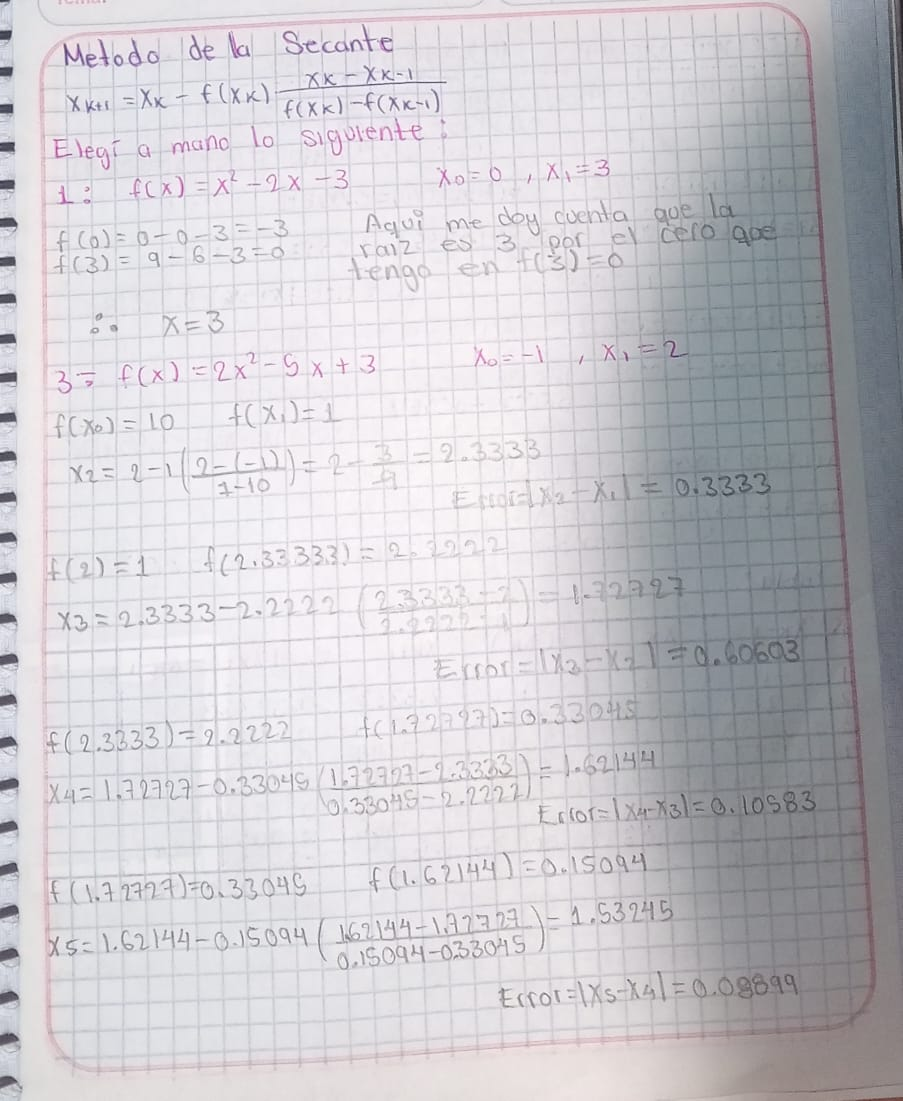
\includegraphics[width=2.60417in,height=\textheight,keepaspectratio,alt={pag.1}]{SECANTE_1.jpg}
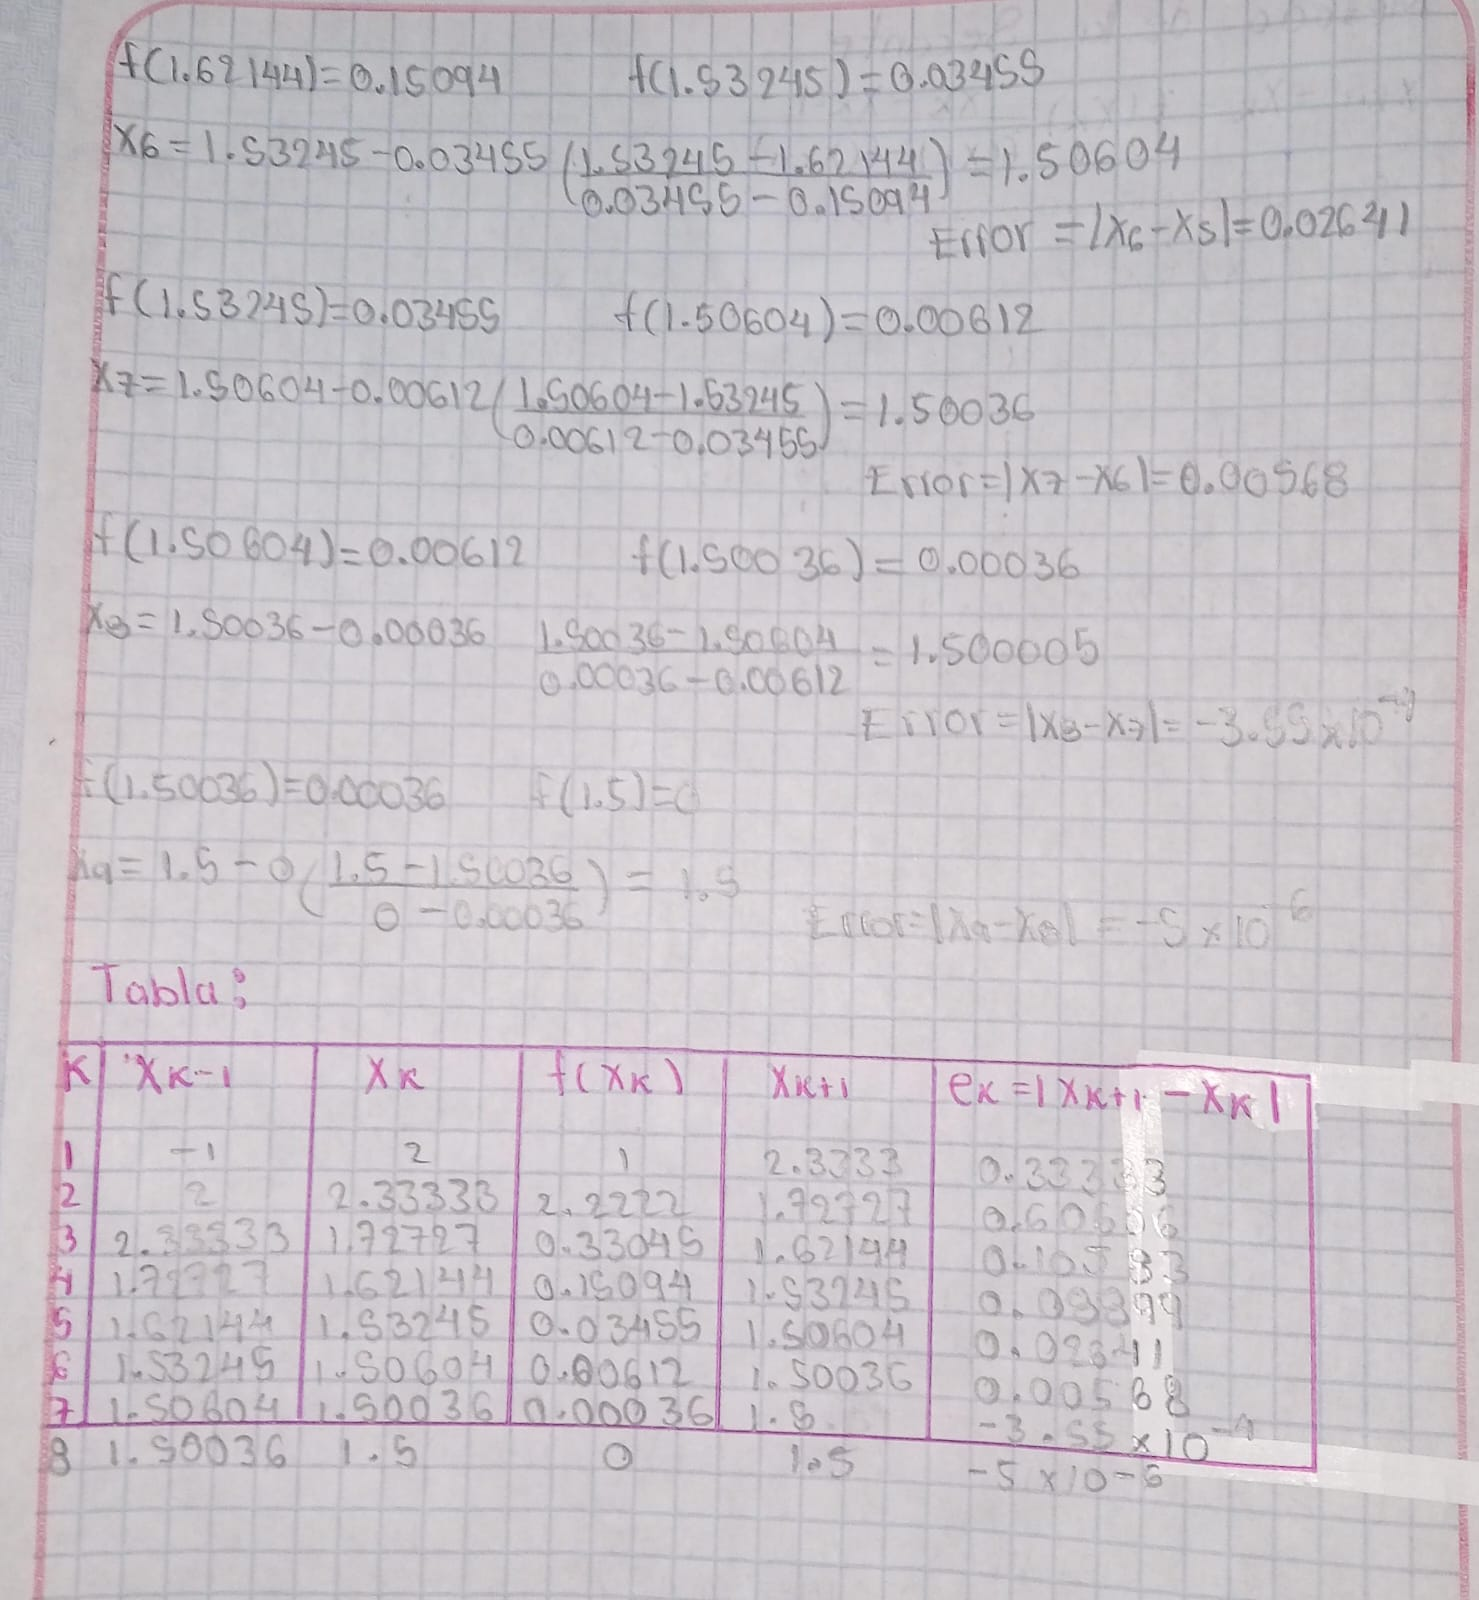
\includegraphics[width=2.60417in,height=\textheight,keepaspectratio,alt={pag.1}]{SECANTE_2.jpg}
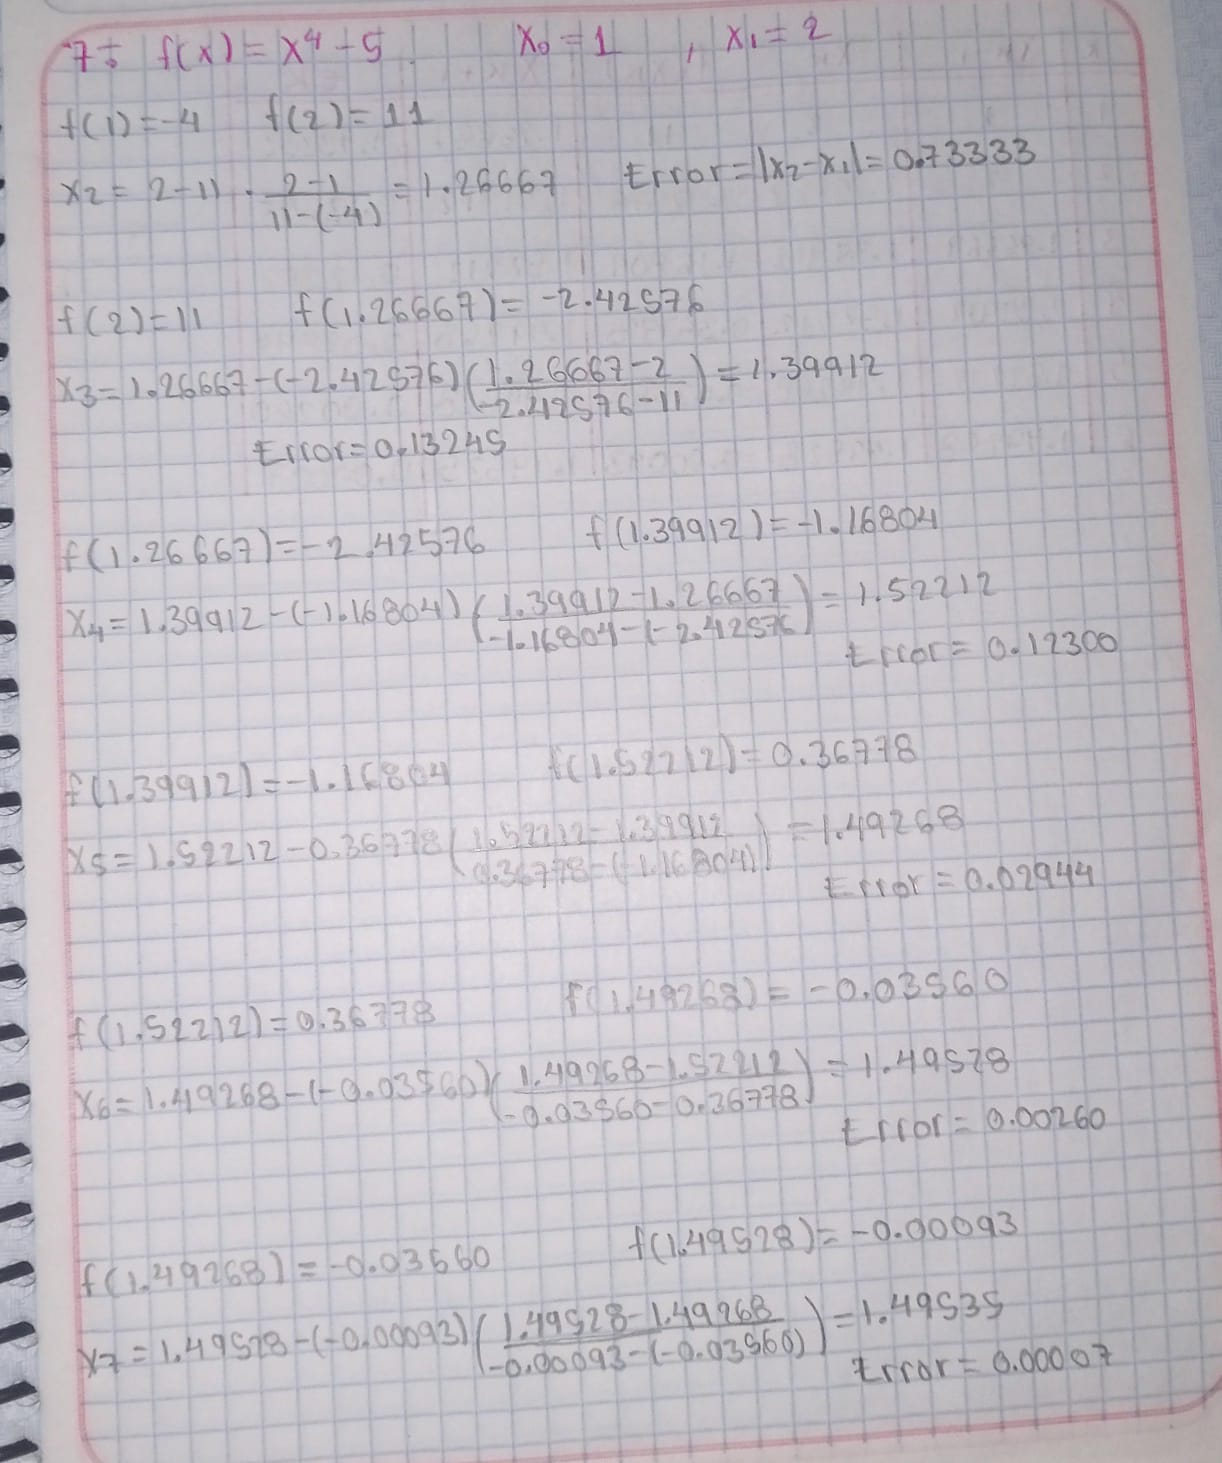
\includegraphics[width=2.60417in,height=\textheight,keepaspectratio,alt={pag.1}]{SECANTE_3.jpg}
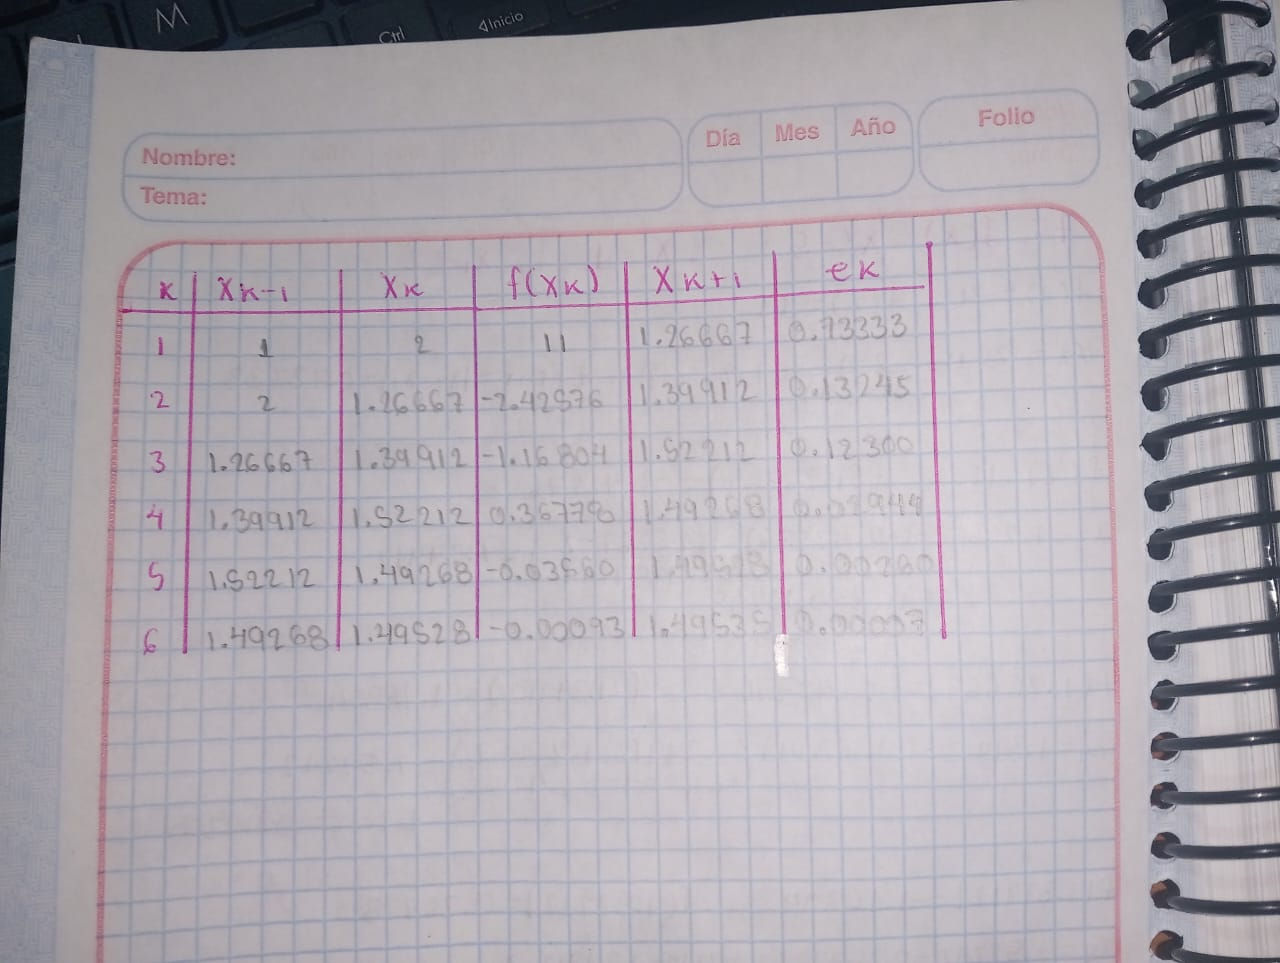
\includegraphics[width=2.60417in,height=\textheight,keepaspectratio,alt={pag.1}]{SECANTE_4.jpg}

\subsection{\texorpdfstring{\emph{Ejercicios en
código:}}{Ejercicios en código:}}\label{ejercicios-en-cuxf3digo-1}

\begin{Shaded}
\begin{Highlighting}[]
\NormalTok{metodo\_secante }\OtherTok{\textless{}{-}} \ControlFlowTok{function}\NormalTok{(f, x0, x1, }\AttributeTok{tol =} \FloatTok{1e{-}5}\NormalTok{, }\AttributeTok{iter\_max =} \DecValTok{100}\NormalTok{) \{}
\NormalTok{  iter }\OtherTok{\textless{}{-}} \DecValTok{0}
\NormalTok{  error }\OtherTok{\textless{}{-}} \DecValTok{1}
  
\NormalTok{  resultados }\OtherTok{\textless{}{-}} \FunctionTok{data.frame}\NormalTok{(}
    \AttributeTok{k =} \FunctionTok{integer}\NormalTok{(),}
    \AttributeTok{x\_k1 =} \FunctionTok{numeric}\NormalTok{(),}
    \AttributeTok{x\_k =} \FunctionTok{numeric}\NormalTok{(),}
    \AttributeTok{f\_x\_k =} \FunctionTok{numeric}\NormalTok{(),}
    \AttributeTok{x\_kp1 =} \FunctionTok{numeric}\NormalTok{(),}
    \AttributeTok{e\_k =} \FunctionTok{numeric}\NormalTok{()}
\NormalTok{  )}
  
\NormalTok{  x\_prev }\OtherTok{\textless{}{-}}\NormalTok{ x0}
\NormalTok{  x\_curr }\OtherTok{\textless{}{-}}\NormalTok{ x1}
  
  \FunctionTok{cat}\NormalTok{(}\StringTok{"Método de la Secante para f(x) ="}\NormalTok{, }\FunctionTok{deparse}\NormalTok{(}\FunctionTok{body}\NormalTok{(f)), }\StringTok{"}\SpecialCharTok{\textbackslash{}n}\StringTok{"}\NormalTok{)}
  \FunctionTok{cat}\NormalTok{(}\StringTok{"x0 ="}\NormalTok{, x0, }\StringTok{", x1 ="}\NormalTok{, x1, }\StringTok{"}\SpecialCharTok{\textbackslash{}n}\StringTok{"}\NormalTok{)}
  \FunctionTok{cat}\NormalTok{(}\StringTok{"Tolerancia ="}\NormalTok{, tol, }\StringTok{"}\SpecialCharTok{\textbackslash{}n\textbackslash{}n}\StringTok{"}\NormalTok{)}
  
  \ControlFlowTok{while}\NormalTok{ (error }\SpecialCharTok{\textgreater{}}\NormalTok{ tol }\SpecialCharTok{\&\&}\NormalTok{ iter }\SpecialCharTok{\textless{}}\NormalTok{ iter\_max) \{}
\NormalTok{    f\_prev }\OtherTok{\textless{}{-}} \FunctionTok{f}\NormalTok{(x\_prev)}
\NormalTok{    f\_curr }\OtherTok{\textless{}{-}} \FunctionTok{f}\NormalTok{(x\_curr)}
    
    \ControlFlowTok{if}\NormalTok{ (}\FunctionTok{abs}\NormalTok{(f\_curr }\SpecialCharTok{{-}}\NormalTok{ f\_prev) }\SpecialCharTok{\textless{}} \FloatTok{1e{-}12}\NormalTok{) \{}
      \FunctionTok{cat}\NormalTok{(}\StringTok{"Error: División por cero}\SpecialCharTok{\textbackslash{}n}\StringTok{"}\NormalTok{)}
      \FunctionTok{return}\NormalTok{(}\ConstantTok{NA}\NormalTok{)}
\NormalTok{    \}}
    
\NormalTok{    x\_next }\OtherTok{\textless{}{-}}\NormalTok{ x\_curr }\SpecialCharTok{{-}}\NormalTok{ f\_curr }\SpecialCharTok{*}\NormalTok{ (x\_curr }\SpecialCharTok{{-}}\NormalTok{ x\_prev) }\SpecialCharTok{/}\NormalTok{ (f\_curr }\SpecialCharTok{{-}}\NormalTok{ f\_prev)}
\NormalTok{    error }\OtherTok{\textless{}{-}} \FunctionTok{abs}\NormalTok{(x\_next }\SpecialCharTok{{-}}\NormalTok{ x\_curr)}
    
\NormalTok{    nueva\_fila }\OtherTok{\textless{}{-}} \FunctionTok{data.frame}\NormalTok{(}
      \AttributeTok{k =}\NormalTok{ iter }\SpecialCharTok{+} \DecValTok{1}\NormalTok{,}
      \AttributeTok{x\_k1 =}\NormalTok{ x\_prev,}
      \AttributeTok{x\_k =}\NormalTok{ x\_curr,}
      \AttributeTok{f\_x\_k =}\NormalTok{ f\_curr,}
      \AttributeTok{x\_kp1 =}\NormalTok{ x\_next,}
      \AttributeTok{e\_k =}\NormalTok{ error}
\NormalTok{    )}
\NormalTok{    resultados }\OtherTok{\textless{}{-}} \FunctionTok{rbind}\NormalTok{(resultados, nueva\_fila)}
    
\NormalTok{    x\_prev }\OtherTok{\textless{}{-}}\NormalTok{ x\_curr}
\NormalTok{    x\_curr }\OtherTok{\textless{}{-}}\NormalTok{ x\_next}
\NormalTok{    iter }\OtherTok{\textless{}{-}}\NormalTok{ iter }\SpecialCharTok{+} \DecValTok{1}
\NormalTok{  \}}
  
  \FunctionTok{cat}\NormalTok{(}\StringTok{"Raíz aproximada:"}\NormalTok{, x\_curr, }\StringTok{"}\SpecialCharTok{\textbackslash{}n}\StringTok{"}\NormalTok{)}
  \FunctionTok{cat}\NormalTok{(}\StringTok{"Iteraciones:"}\NormalTok{, iter, }\StringTok{"}\SpecialCharTok{\textbackslash{}n}\StringTok{"}\NormalTok{)}
  \FunctionTok{cat}\NormalTok{(}\StringTok{"Error final:"}\NormalTok{, error, }\StringTok{"}\SpecialCharTok{\textbackslash{}n\textbackslash{}n}\StringTok{"}\NormalTok{)}
  
  \FunctionTok{return}\NormalTok{(resultados)}
\NormalTok{\}}

\CommentTok{\# FUNCIÓN PARA GRAFICAR}
\NormalTok{graficar\_secante }\OtherTok{\textless{}{-}} \ControlFlowTok{function}\NormalTok{(f, resultados, a, b, titulo) \{}
\NormalTok{  x\_seq }\OtherTok{\textless{}{-}} \FunctionTok{seq}\NormalTok{(a, b, }\AttributeTok{length.out =} \DecValTok{1000}\NormalTok{)}
\NormalTok{  y\_seq }\OtherTok{\textless{}{-}} \FunctionTok{f}\NormalTok{(x\_seq)}
  
  \FunctionTok{plot}\NormalTok{(x\_seq, y\_seq, }\AttributeTok{type =} \StringTok{"l"}\NormalTok{, }\AttributeTok{col =} \StringTok{"blue"}\NormalTok{, }\AttributeTok{lwd =} \DecValTok{2}\NormalTok{,}
       \AttributeTok{main =}\NormalTok{ titulo, }\AttributeTok{xlab =} \StringTok{"x"}\NormalTok{, }\AttributeTok{ylab =} \StringTok{"f(x)"}\NormalTok{)}
  \FunctionTok{abline}\NormalTok{(}\AttributeTok{h =} \DecValTok{0}\NormalTok{, }\AttributeTok{col =} \StringTok{"gray"}\NormalTok{, }\AttributeTok{lty =} \DecValTok{2}\NormalTok{)}
  \FunctionTok{abline}\NormalTok{(}\AttributeTok{v =} \DecValTok{0}\NormalTok{, }\AttributeTok{col =} \StringTok{"gray"}\NormalTok{, }\AttributeTok{lty =} \DecValTok{2}\NormalTok{)}
  
\NormalTok{  n }\OtherTok{\textless{}{-}} \FunctionTok{nrow}\NormalTok{(resultados)}
\NormalTok{  colores }\OtherTok{\textless{}{-}} \FunctionTok{rainbow}\NormalTok{(n)}
  
  \ControlFlowTok{for}\NormalTok{ (i }\ControlFlowTok{in} \DecValTok{1}\SpecialCharTok{:}\NormalTok{n) \{}
\NormalTok{    x\_k1 }\OtherTok{\textless{}{-}}\NormalTok{ resultados}\SpecialCharTok{$}\NormalTok{x\_k1[i]}
\NormalTok{    x\_k }\OtherTok{\textless{}{-}}\NormalTok{ resultados}\SpecialCharTok{$}\NormalTok{x\_k[i]}
\NormalTok{    f\_x\_k1 }\OtherTok{\textless{}{-}} \FunctionTok{f}\NormalTok{(x\_k1)}
\NormalTok{    f\_x\_k }\OtherTok{\textless{}{-}} \FunctionTok{f}\NormalTok{(x\_k)}
    
\NormalTok{    m }\OtherTok{\textless{}{-}}\NormalTok{ (f\_x\_k }\SpecialCharTok{{-}}\NormalTok{ f\_x\_k1) }\SpecialCharTok{/}\NormalTok{ (x\_k }\SpecialCharTok{{-}}\NormalTok{ x\_k1)}
\NormalTok{    b\_linea }\OtherTok{\textless{}{-}}\NormalTok{ f\_x\_k }\SpecialCharTok{{-}}\NormalTok{ m }\SpecialCharTok{*}\NormalTok{ x\_k}
    
\NormalTok{    x\_linea }\OtherTok{\textless{}{-}} \FunctionTok{seq}\NormalTok{(}\FunctionTok{min}\NormalTok{(x\_k1, x\_k) }\SpecialCharTok{{-}} \FloatTok{0.5}\NormalTok{, }\FunctionTok{max}\NormalTok{(x\_k1, x\_k) }\SpecialCharTok{+} \FloatTok{0.5}\NormalTok{, }\AttributeTok{length.out =} \DecValTok{100}\NormalTok{)}
\NormalTok{    y\_linea }\OtherTok{\textless{}{-}}\NormalTok{ m }\SpecialCharTok{*}\NormalTok{ x\_linea }\SpecialCharTok{+}\NormalTok{ b\_linea}
    
    \FunctionTok{lines}\NormalTok{(x\_linea, y\_linea, }\AttributeTok{col =}\NormalTok{ colores[i], }\AttributeTok{lwd =} \DecValTok{1}\NormalTok{, }\AttributeTok{lty =} \DecValTok{2}\NormalTok{)}
    \FunctionTok{points}\NormalTok{(}\FunctionTok{c}\NormalTok{(x\_k1, x\_k), }\FunctionTok{c}\NormalTok{(f\_x\_k1, f\_x\_k), }\AttributeTok{col =}\NormalTok{ colores[i], }\AttributeTok{pch =} \DecValTok{19}\NormalTok{, }\AttributeTok{cex =} \FloatTok{0.8}\NormalTok{)}
    
    \ControlFlowTok{if}\NormalTok{ (i }\SpecialCharTok{\textless{}}\NormalTok{ n) \{}
\NormalTok{      x\_next }\OtherTok{\textless{}{-}}\NormalTok{ resultados}\SpecialCharTok{$}\NormalTok{x\_kp1[i]}
      \FunctionTok{points}\NormalTok{(x\_next, }\DecValTok{0}\NormalTok{, }\AttributeTok{col =}\NormalTok{ colores[i], }\AttributeTok{pch =} \DecValTok{17}\NormalTok{, }\AttributeTok{cex =} \FloatTok{1.2}\NormalTok{)}
\NormalTok{    \}}
\NormalTok{  \}}
  
\NormalTok{  raiz\_final }\OtherTok{\textless{}{-}}\NormalTok{ resultados}\SpecialCharTok{$}\NormalTok{x\_kp1[n]}
  \FunctionTok{points}\NormalTok{(raiz\_final, }\DecValTok{0}\NormalTok{, }\AttributeTok{col =} \StringTok{"red"}\NormalTok{, }\AttributeTok{pch =} \DecValTok{17}\NormalTok{, }\AttributeTok{cex =} \DecValTok{2}\NormalTok{)}
  \FunctionTok{text}\NormalTok{(raiz\_final, }\DecValTok{0}\NormalTok{, }\StringTok{"Raíz"}\NormalTok{, }\AttributeTok{pos =} \DecValTok{3}\NormalTok{, }\AttributeTok{col =} \StringTok{"red"}\NormalTok{)}
\NormalTok{\}}
\end{Highlighting}
\end{Shaded}

\subsection{Ejercicio 2:}\label{ejercicio-2}

\(f(x) = x^4 - 10x^2 + 9\) con \(x_0 = 0\), \(x_1 = 2\)

\begin{Shaded}
\begin{Highlighting}[]
\NormalTok{f2 }\OtherTok{\textless{}{-}} \ControlFlowTok{function}\NormalTok{(x) x}\SpecialCharTok{\^{}}\DecValTok{4} \SpecialCharTok{{-}} \DecValTok{10}\SpecialCharTok{*}\NormalTok{x}\SpecialCharTok{\^{}}\DecValTok{2} \SpecialCharTok{+} \DecValTok{9}
\NormalTok{resultado2 }\OtherTok{\textless{}{-}} \FunctionTok{metodo\_secante}\NormalTok{(f2, }\AttributeTok{x0 =} \DecValTok{0}\NormalTok{, }\AttributeTok{x1 =} \DecValTok{2}\NormalTok{)}
\end{Highlighting}
\end{Shaded}

\begin{verbatim}
## Método de la Secante para f(x) = x^4 - 10 * x^2 + 9 
## x0 = 0 , x1 = 2 
## Tolerancia = 1e-05 
## 
## Raíz aproximada: 1 
## Iteraciones: 5 
## Error final: 2.068098e-07
\end{verbatim}

\begin{Shaded}
\begin{Highlighting}[]
\NormalTok{knitr}\SpecialCharTok{::}\FunctionTok{kable}\NormalTok{(resultado2, }\AttributeTok{digits =} \DecValTok{6}\NormalTok{, }\AttributeTok{caption =} \StringTok{"Iteraciones del método de la secante para f(x) = x⁴ {-} 10x² + 9"}\NormalTok{)}
\end{Highlighting}
\end{Shaded}

\begin{longtable}[]{@{}rrrrrr@{}}
\caption{Iteraciones del método de la secante para f(x) = x⁴ - 10x² +
9}\tabularnewline
\toprule\noalign{}
k & x\_k1 & x\_k & f\_x\_k & x\_kp1 & e\_k \\
\midrule\noalign{}
\endfirsthead
\toprule\noalign{}
k & x\_k1 & x\_k & f\_x\_k & x\_kp1 & e\_k \\
\midrule\noalign{}
\endhead
\bottomrule\noalign{}
\endlastfoot
1 & 0.000000 & 2.000000 & -15.000000 & 0.750000 & 1.250000 \\
2 & 2.000000 & 0.750000 & 3.691406 & 0.996865 & 0.246865 \\
3 & 0.750000 & 0.996865 & 0.050117 & 1.000263 & 0.003398 \\
4 & 0.996865 & 1.000263 & -0.004208 & 1.000000 & 0.000263 \\
5 & 1.000263 & 1.000000 & 0.000003 & 1.000000 & 0.000000 \\
\end{longtable}

\begin{Shaded}
\begin{Highlighting}[]
\FunctionTok{graficar\_secante}\NormalTok{(f2, resultado2, }\SpecialCharTok{{-}}\DecValTok{1}\NormalTok{, }\DecValTok{3}\NormalTok{, }\StringTok{"Método de la Secante {-} Ejercicio 2: f(x) = x⁴ {-} 10x² + 9"}\NormalTok{)}
\end{Highlighting}
\end{Shaded}

\pandocbounded{\includegraphics[keepaspectratio]{Notas_MN_LILIANA_CS_files/figure-latex/unnamed-chunk-454-1.pdf}}

\subsection{Ejercicio 4:}\label{ejercicio-4}

\(f(x) = -3x^2 + 4x + 2\) con \(x_0 = -1\), \(x_1 = 3\)

\begin{Shaded}
\begin{Highlighting}[]
\NormalTok{f4 }\OtherTok{\textless{}{-}} \ControlFlowTok{function}\NormalTok{(x) }\SpecialCharTok{{-}}\DecValTok{3}\SpecialCharTok{*}\NormalTok{x}\SpecialCharTok{\^{}}\DecValTok{2} \SpecialCharTok{+} \DecValTok{4}\SpecialCharTok{*}\NormalTok{x }\SpecialCharTok{+} \DecValTok{2}
\NormalTok{resultado4 }\OtherTok{\textless{}{-}} \FunctionTok{metodo\_secante}\NormalTok{(f4, }\AttributeTok{x0 =} \SpecialCharTok{{-}}\DecValTok{1}\NormalTok{, }\AttributeTok{x1 =} \DecValTok{3}\NormalTok{)}
\end{Highlighting}
\end{Shaded}

\begin{verbatim}
## Método de la Secante para f(x) = -3 * x^2 + 4 * x + 2 
## x0 = -1 , x1 = 3 
## Tolerancia = 1e-05 
## 
## Raíz aproximada: 1.720759 
## Iteraciones: 14 
## Error final: 5.739036e-09
\end{verbatim}

\begin{Shaded}
\begin{Highlighting}[]
\NormalTok{knitr}\SpecialCharTok{::}\FunctionTok{kable}\NormalTok{(resultado4, }\AttributeTok{digits =} \DecValTok{6}\NormalTok{, }\AttributeTok{caption =} \StringTok{"Iteraciones del método de la secante para f(x) = {-}3x² + 4x + 2"}\NormalTok{)}
\end{Highlighting}
\end{Shaded}

\begin{longtable}[]{@{}rrrrrr@{}}
\caption{Iteraciones del método de la secante para f(x) = -3x² + 4x +
2}\tabularnewline
\toprule\noalign{}
k & x\_k1 & x\_k & f\_x\_k & x\_kp1 & e\_k \\
\midrule\noalign{}
\endfirsthead
\toprule\noalign{}
k & x\_k1 & x\_k & f\_x\_k & x\_kp1 & e\_k \\
\midrule\noalign{}
\endhead
\bottomrule\noalign{}
\endlastfoot
1 & -1.000000 & 3.000000 & -13.000000 & -3.500000 & 6.500000 \\
2 & 3.000000 & -3.500000 & -48.750000 & 5.363636 & 8.863636 \\
3 & -3.500000 & 5.363636 & -62.851240 & -34.142857 & 39.506494 \\
4 & 5.363636 & -34.142857 & -3631.775510 & 6.059373 & 40.202230 \\
5 & -34.142857 & 6.059373 & -83.910518 & 7.010196 & 0.950823 \\
6 & 6.059373 & 7.010196 & -117.387750 & 3.676141 & 3.334055 \\
7 & 7.010196 & 3.676141 & -23.837477 & 2.826593 & 0.849548 \\
8 & 3.676141 & 2.826593 & -10.662514 & 2.139053 & 0.687540 \\
9 & 2.826593 & 2.139053 & -3.170430 & 1.848106 & 0.290947 \\
10 & 2.139053 & 1.848106 & -0.854063 & 1.740832 & 0.107274 \\
11 & 1.848106 & 1.740832 & -0.128157 & 1.721892 & 0.018939 \\
12 & 1.740832 & 1.721892 & -0.007171 & 1.720770 & 0.001123 \\
13 & 1.721892 & 1.720770 & -0.000068 & 1.720759 & 0.000011 \\
14 & 1.720770 & 1.720759 & 0.000000 & 1.720759 & 0.000000 \\
\end{longtable}

\begin{Shaded}
\begin{Highlighting}[]
\FunctionTok{graficar\_secante}\NormalTok{(f4, resultado4, }\SpecialCharTok{{-}}\DecValTok{2}\NormalTok{, }\DecValTok{4}\NormalTok{, }\StringTok{"Método de la Secante {-} Ejercicio 4: f(x) = {-}3x² + 4x + 2"}\NormalTok{)}
\end{Highlighting}
\end{Shaded}

\pandocbounded{\includegraphics[keepaspectratio]{Notas_MN_LILIANA_CS_files/figure-latex/unnamed-chunk-456-1.pdf}}

\subsection{Ejercicio 8:}\label{ejercicio-8}

\(f(x) = -2x^4 + 3x^3 + 7x^2 - 5x + 1\) con \(x_0 = 2\), \(x_1 = 4\)

\begin{Shaded}
\begin{Highlighting}[]
\NormalTok{f8 }\OtherTok{\textless{}{-}} \ControlFlowTok{function}\NormalTok{(x) }\SpecialCharTok{{-}}\DecValTok{2}\SpecialCharTok{*}\NormalTok{x}\SpecialCharTok{\^{}}\DecValTok{4} \SpecialCharTok{+} \DecValTok{3}\SpecialCharTok{*}\NormalTok{x}\SpecialCharTok{\^{}}\DecValTok{3} \SpecialCharTok{+} \DecValTok{7}\SpecialCharTok{*}\NormalTok{x}\SpecialCharTok{\^{}}\DecValTok{2} \SpecialCharTok{{-}} \DecValTok{5}\SpecialCharTok{*}\NormalTok{x }\SpecialCharTok{+} \DecValTok{1}
\NormalTok{resultado8 }\OtherTok{\textless{}{-}} \FunctionTok{metodo\_secante}\NormalTok{(f8, }\AttributeTok{x0 =} \DecValTok{2}\NormalTok{, }\AttributeTok{x1 =} \DecValTok{4}\NormalTok{)}
\end{Highlighting}
\end{Shaded}

\begin{verbatim}
## Método de la Secante para f(x) = -2 * x^4 + 3 * x^3 + 7 * x^2 - 5 * x + 1 
## x0 = 2 , x1 = 4 
## Tolerancia = 1e-05 
## 
## Raíz aproximada: 2.525062 
## Iteraciones: 10 
## Error final: 1.469183e-08
\end{verbatim}

\begin{Shaded}
\begin{Highlighting}[]
\NormalTok{knitr}\SpecialCharTok{::}\FunctionTok{kable}\NormalTok{(resultado8, }\AttributeTok{digits =} \DecValTok{6}\NormalTok{, }\AttributeTok{caption =} \StringTok{"Iteraciones del método de la secante para f(x) = {-}2x⁴ + 3x³ + 7x² {-} 5x + 1"}\NormalTok{)}
\end{Highlighting}
\end{Shaded}

\begin{longtable}[]{@{}rrrrrr@{}}
\caption{Iteraciones del método de la secante para f(x) = -2x⁴ + 3x³ +
7x² - 5x + 1}\tabularnewline
\toprule\noalign{}
k & x\_k1 & x\_k & f\_x\_k & x\_kp1 & e\_k \\
\midrule\noalign{}
\endfirsthead
\toprule\noalign{}
k & x\_k1 & x\_k & f\_x\_k & x\_kp1 & e\_k \\
\midrule\noalign{}
\endhead
\bottomrule\noalign{}
\endlastfoot
1 & 2.000000 & 4.000000 & -227.000000 & 2.092437 & 1.907563 \\
2 & 4.000000 & 2.092437 & 10.330876 & 2.175472 & 0.083035 \\
3 & 2.092437 & 2.175472 & 9.342326 & 2.960198 & 0.784726 \\
4 & 2.175472 & 2.960198 & -28.215357 & 2.370670 & 0.589529 \\
5 & 2.960198 & 2.370670 & 5.286717 & 2.463699 & 0.093029 \\
6 & 2.370670 & 2.463699 & 2.347519 & 2.538001 & 0.074302 \\
7 & 2.463699 & 2.538001 & -0.539170 & 2.524123 & 0.013878 \\
8 & 2.538001 & 2.524123 & 0.038526 & 2.525048 & 0.000926 \\
9 & 2.524123 & 2.525048 & 0.000563 & 2.525062 & 0.000014 \\
10 & 2.525048 & 2.525062 & -0.000001 & 2.525062 & 0.000000 \\
\end{longtable}

\begin{Shaded}
\begin{Highlighting}[]
\FunctionTok{graficar\_secante}\NormalTok{(f8, resultado8, }\DecValTok{0}\NormalTok{, }\DecValTok{3}\NormalTok{, }\StringTok{"Método de la Secante {-} Ejercicio 8: f(x) = {-}2x⁴ + 3x³ + 7x² {-} 5x + 1"}\NormalTok{)}
\end{Highlighting}
\end{Shaded}

\pandocbounded{\includegraphics[keepaspectratio]{Notas_MN_LILIANA_CS_files/figure-latex/unnamed-chunk-458-1.pdf}}

\subsection{Ejercicio 11:}\label{ejercicio-11}

\(f(x) = \sin(x) - \frac{x}{3}\) con \(x_0 = 0\), \(x_1 = 1\)

\begin{Shaded}
\begin{Highlighting}[]
\NormalTok{f11 }\OtherTok{\textless{}{-}} \ControlFlowTok{function}\NormalTok{(x) }\FunctionTok{sin}\NormalTok{(x) }\SpecialCharTok{{-}}\NormalTok{ x}\SpecialCharTok{/}\DecValTok{3}
\NormalTok{resultado11 }\OtherTok{\textless{}{-}} \FunctionTok{metodo\_secante}\NormalTok{(f11, }\AttributeTok{x0 =} \DecValTok{0}\NormalTok{, }\AttributeTok{x1 =} \DecValTok{1}\NormalTok{)}
\end{Highlighting}
\end{Shaded}

\begin{verbatim}
## Método de la Secante para f(x) = sin(x) - x/3 
## x0 = 0 , x1 = 1 
## Tolerancia = 1e-05 
## 
## Raíz aproximada: 0 
## Iteraciones: 2 
## Error final: 0
\end{verbatim}

\begin{Shaded}
\begin{Highlighting}[]
\NormalTok{knitr}\SpecialCharTok{::}\FunctionTok{kable}\NormalTok{(resultado11, }\AttributeTok{digits =} \DecValTok{6}\NormalTok{, }\AttributeTok{caption =} \StringTok{"Iteraciones del método de la secante para f(x) = sin(x) {-} x/3"}\NormalTok{)}
\end{Highlighting}
\end{Shaded}

\begin{longtable}[]{@{}rrrrrr@{}}
\caption{Iteraciones del método de la secante para f(x) = sin(x) -
x/3}\tabularnewline
\toprule\noalign{}
k & x\_k1 & x\_k & f\_x\_k & x\_kp1 & e\_k \\
\midrule\noalign{}
\endfirsthead
\toprule\noalign{}
k & x\_k1 & x\_k & f\_x\_k & x\_kp1 & e\_k \\
\midrule\noalign{}
\endhead
\bottomrule\noalign{}
\endlastfoot
1 & 0 & 1 & 0.508138 & 0 & 1 \\
2 & 1 & 0 & 0.000000 & 0 & 0 \\
\end{longtable}

\begin{Shaded}
\begin{Highlighting}[]
\FunctionTok{graficar\_secante}\NormalTok{(f11, resultado11, }\SpecialCharTok{{-}}\DecValTok{1}\NormalTok{, }\DecValTok{2}\NormalTok{, }\StringTok{"Método de la Secante {-} Ejercicio 11: f(x) = sin(x) {-} x/3"}\NormalTok{)}
\end{Highlighting}
\end{Shaded}

\pandocbounded{\includegraphics[keepaspectratio]{Notas_MN_LILIANA_CS_files/figure-latex/unnamed-chunk-460-1.pdf}}

\subsection{Ejercicio 12:}\label{ejercicio-12}

\(f(x) = (3x + 3.1)\cos(2x + \pi/6)\) con \(x_0 = 0.3\), \(x_1 = 0.8\)

\begin{Shaded}
\begin{Highlighting}[]
\NormalTok{f12 }\OtherTok{\textless{}{-}} \ControlFlowTok{function}\NormalTok{(x) (}\DecValTok{3}\SpecialCharTok{*}\NormalTok{x }\SpecialCharTok{+} \FloatTok{3.1}\NormalTok{) }\SpecialCharTok{*} \FunctionTok{cos}\NormalTok{(}\DecValTok{2}\SpecialCharTok{*}\NormalTok{x }\SpecialCharTok{+}\NormalTok{ pi}\SpecialCharTok{/}\DecValTok{6}\NormalTok{)}
\NormalTok{resultado12 }\OtherTok{\textless{}{-}} \FunctionTok{metodo\_secante}\NormalTok{(f12, }\AttributeTok{x0 =} \FloatTok{0.3}\NormalTok{, }\AttributeTok{x1 =} \FloatTok{0.8}\NormalTok{)}
\end{Highlighting}
\end{Shaded}

\begin{verbatim}
## Método de la Secante para f(x) = (3 * x + 3.1) * cos(2 * x + pi/6) 
## x0 = 0.3 , x1 = 0.8 
## Tolerancia = 1e-05 
## 
## Raíz aproximada: 0.5235988 
## Iteraciones: 5 
## Error final: 2.782563e-07
\end{verbatim}

\begin{Shaded}
\begin{Highlighting}[]
\NormalTok{knitr}\SpecialCharTok{::}\FunctionTok{kable}\NormalTok{(resultado12, }\AttributeTok{digits =} \DecValTok{6}\NormalTok{, }\AttributeTok{caption =} \StringTok{"Iteraciones del método de la secante para f(x) = (3x + 3.1)cos(2x + π/6)"}\NormalTok{)}
\end{Highlighting}
\end{Shaded}

\begin{longtable}[]{@{}rrrrrr@{}}
\caption{Iteraciones del método de la secante para f(x) = (3x +
3.1)cos(2x + π/6)}\tabularnewline
\toprule\noalign{}
k & x\_k1 & x\_k & f\_x\_k & x\_kp1 & e\_k \\
\midrule\noalign{}
\endfirsthead
\toprule\noalign{}
k & x\_k1 & x\_k & f\_x\_k & x\_kp1 & e\_k \\
\midrule\noalign{}
\endhead
\bottomrule\noalign{}
\endlastfoot
1 & 0.300000 & 0.800000 & -2.887909 & 0.487298 & 0.312702 \\
2 & 0.800000 & 0.487298 & 0.330909 & 0.519445 & 0.032147 \\
3 & 0.487298 & 0.519445 & 0.038697 & 0.523702 & 0.004257 \\
4 & 0.519445 & 0.523702 & -0.000968 & 0.523598 & 0.000104 \\
5 & 0.523702 & 0.523598 & 0.000003 & 0.523599 & 0.000000 \\
\end{longtable}

\begin{Shaded}
\begin{Highlighting}[]
\FunctionTok{graficar\_secante}\NormalTok{(f12, resultado12, }\DecValTok{0}\NormalTok{, }\FloatTok{1.5}\NormalTok{, }\StringTok{"Método de la Secante {-} Ejercicio 12: f(x) = (3x + 3.1)cos(2x + π/6)"}\NormalTok{)}
\end{Highlighting}
\end{Shaded}

\pandocbounded{\includegraphics[keepaspectratio]{Notas_MN_LILIANA_CS_files/figure-latex/unnamed-chunk-462-1.pdf}}

\section{\texorpdfstring{\textbf{Método de
Newton}}{Método de Newton}}\label{muxe9todo-de-newton}

\subsection{\texorpdfstring{\emph{Ejercicios a
mano}}{Ejercicios a mano}}\label{ejercicios-a-mano-3}

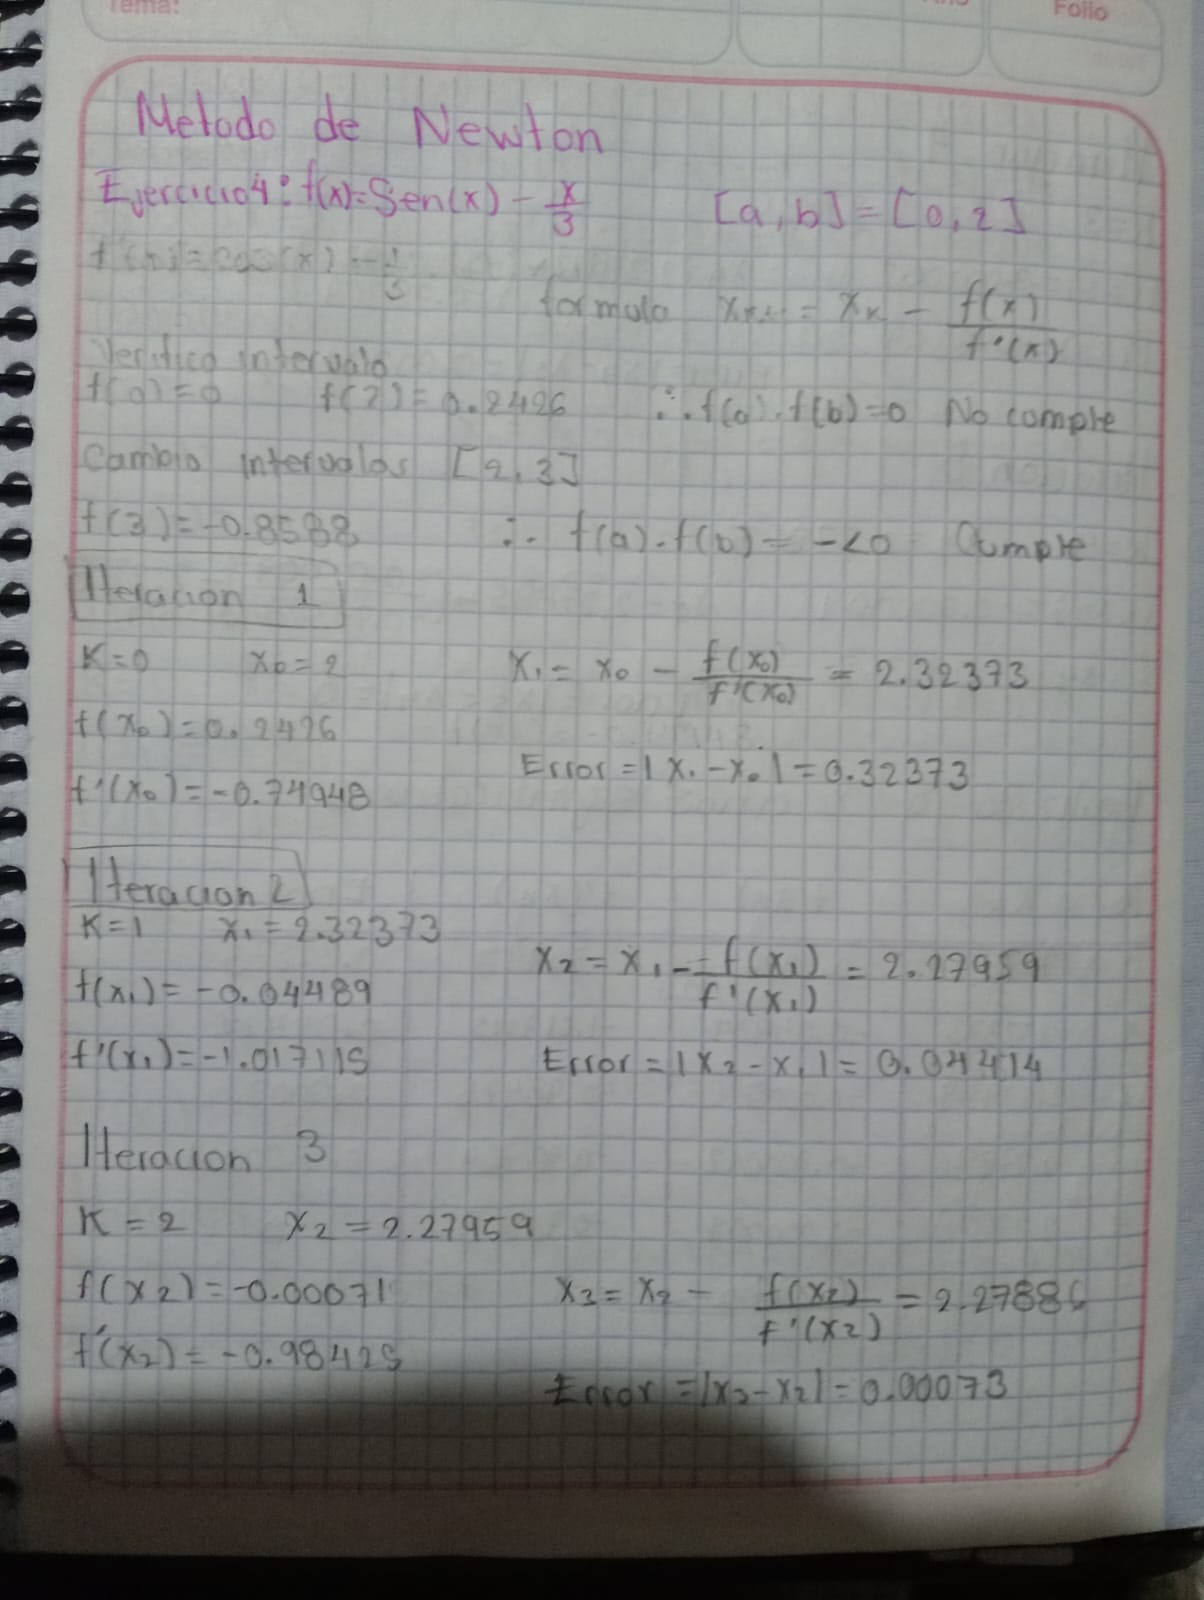
\includegraphics[width=2.60417in,height=\textheight,keepaspectratio,alt={pag.1}]{Newton _1.jpg}
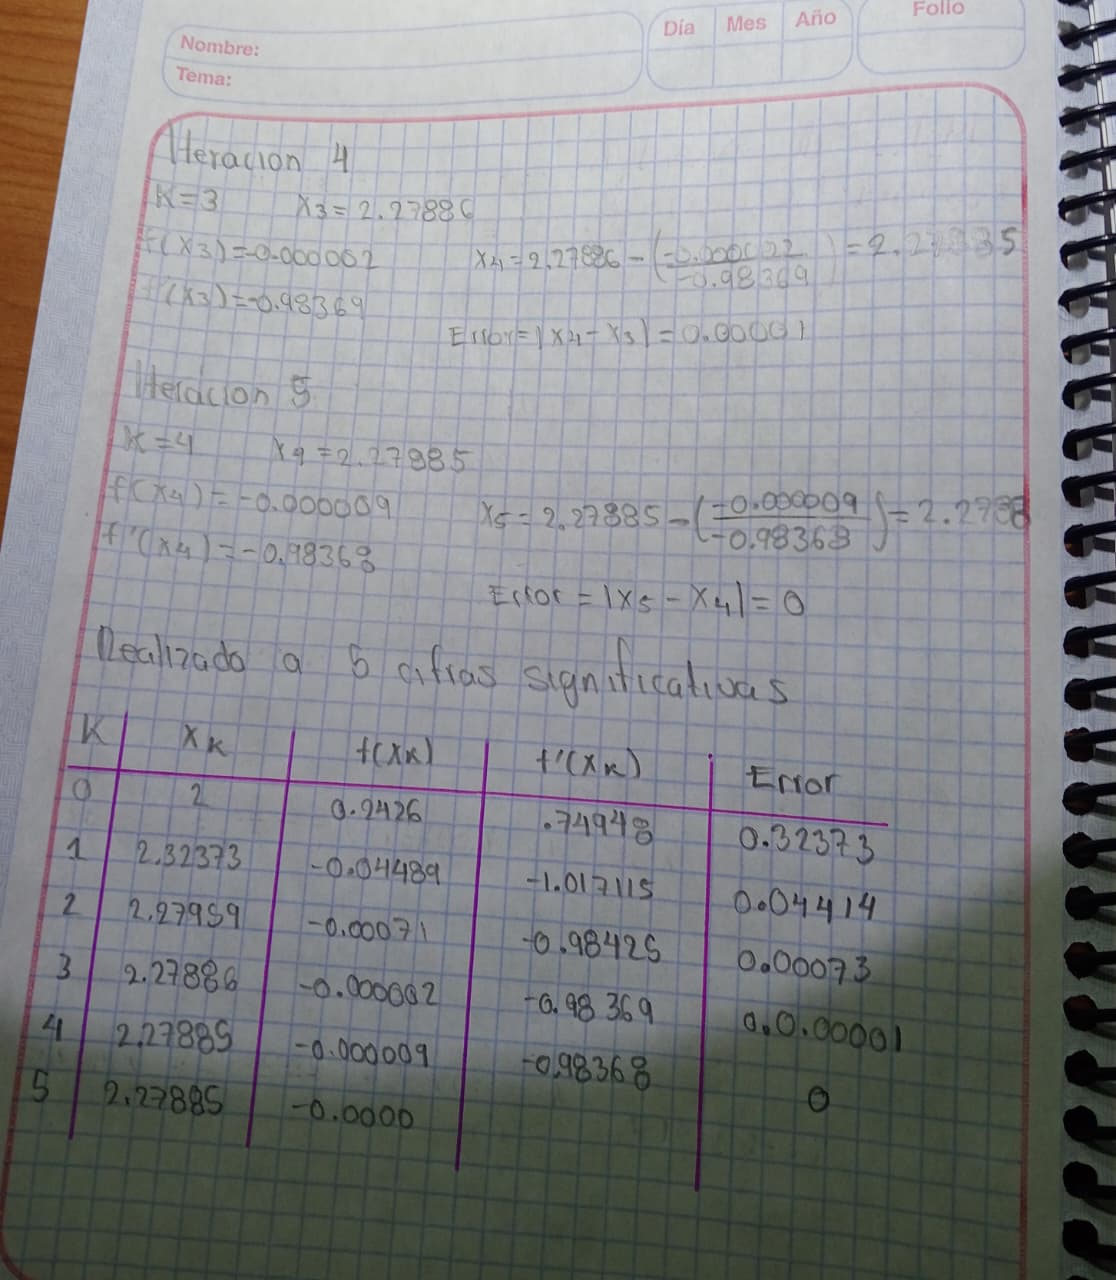
\includegraphics[width=2.60417in,height=\textheight,keepaspectratio,alt={pag.1}]{Newton _2.jpg}
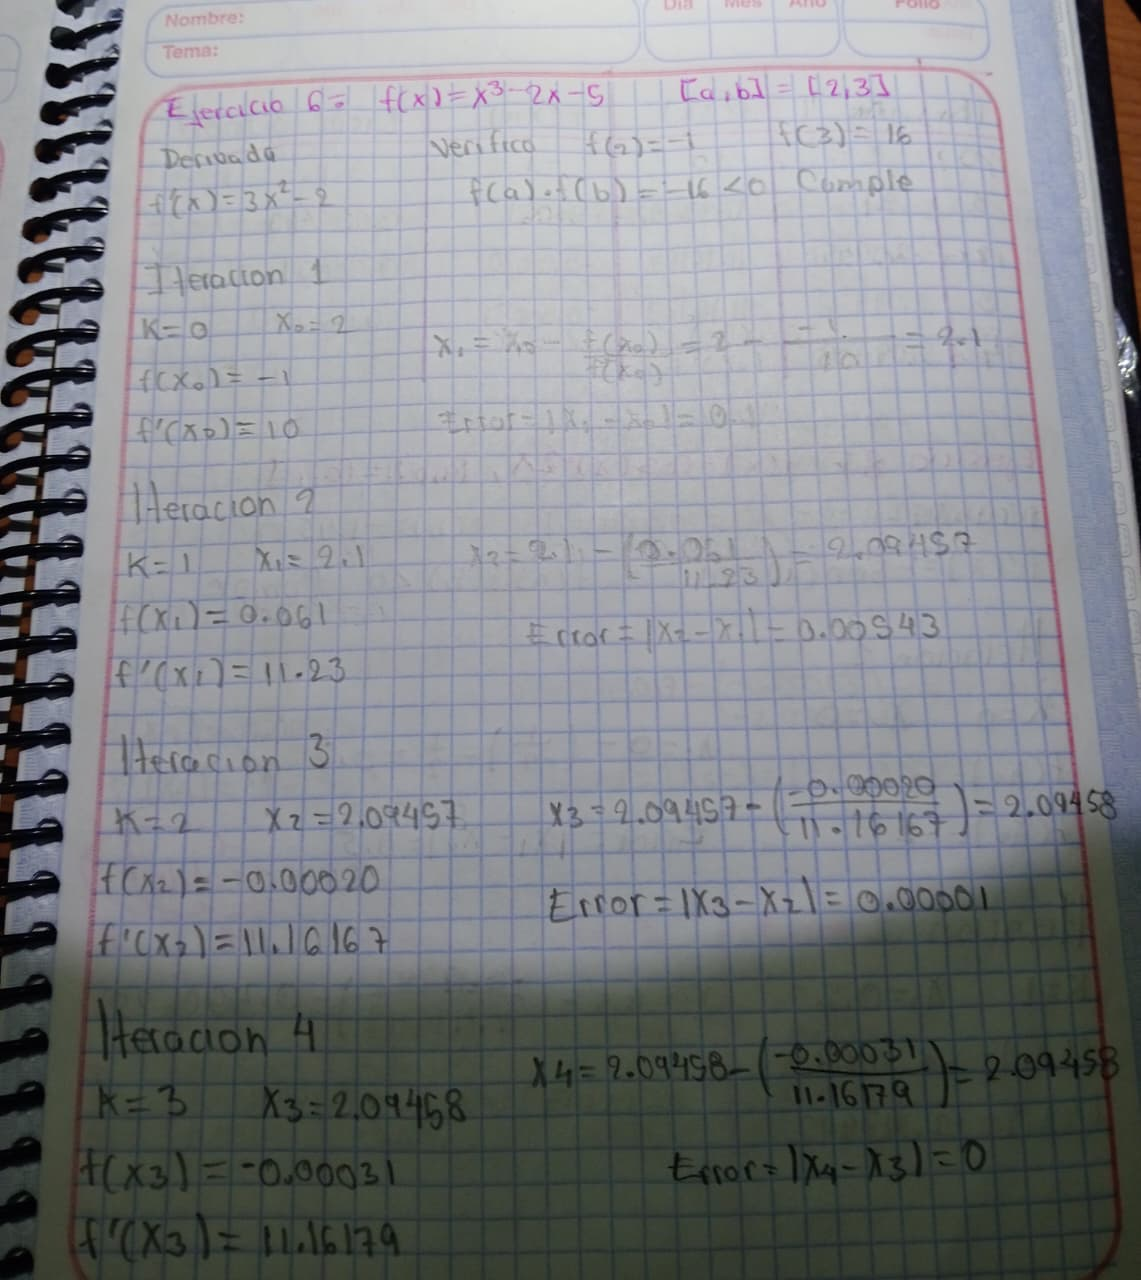
\includegraphics[width=2.60417in,height=\textheight,keepaspectratio,alt={pag.1}]{Newton _3.jpg}
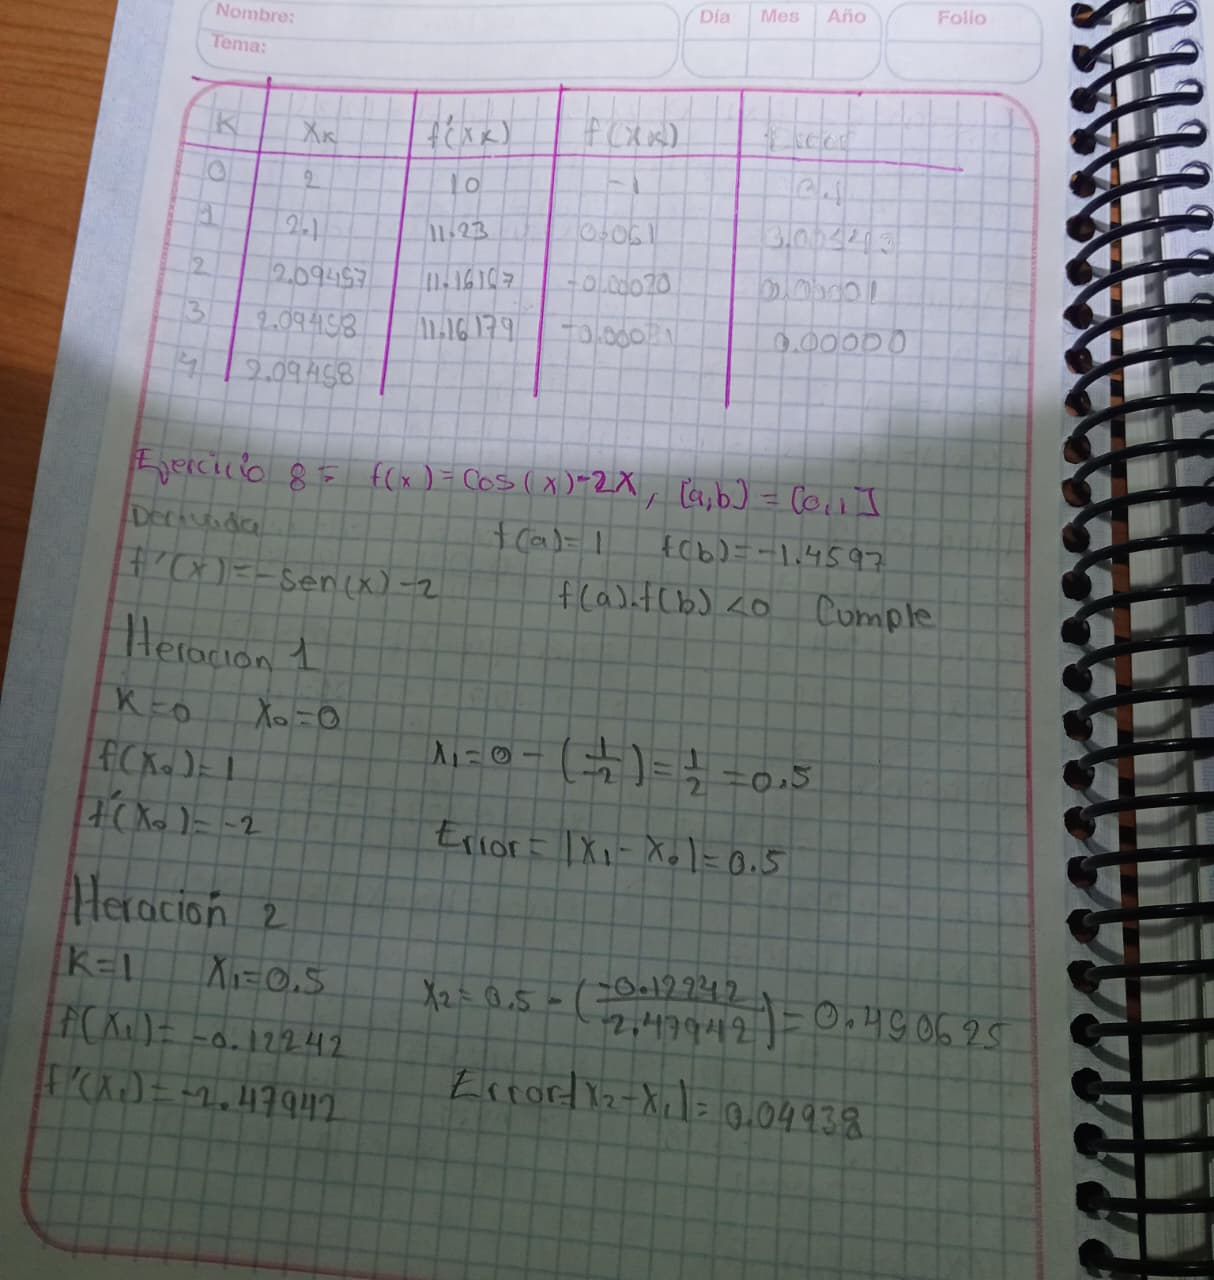
\includegraphics[width=2.60417in,height=\textheight,keepaspectratio,alt={pag.1}]{Newton _4.jpg}
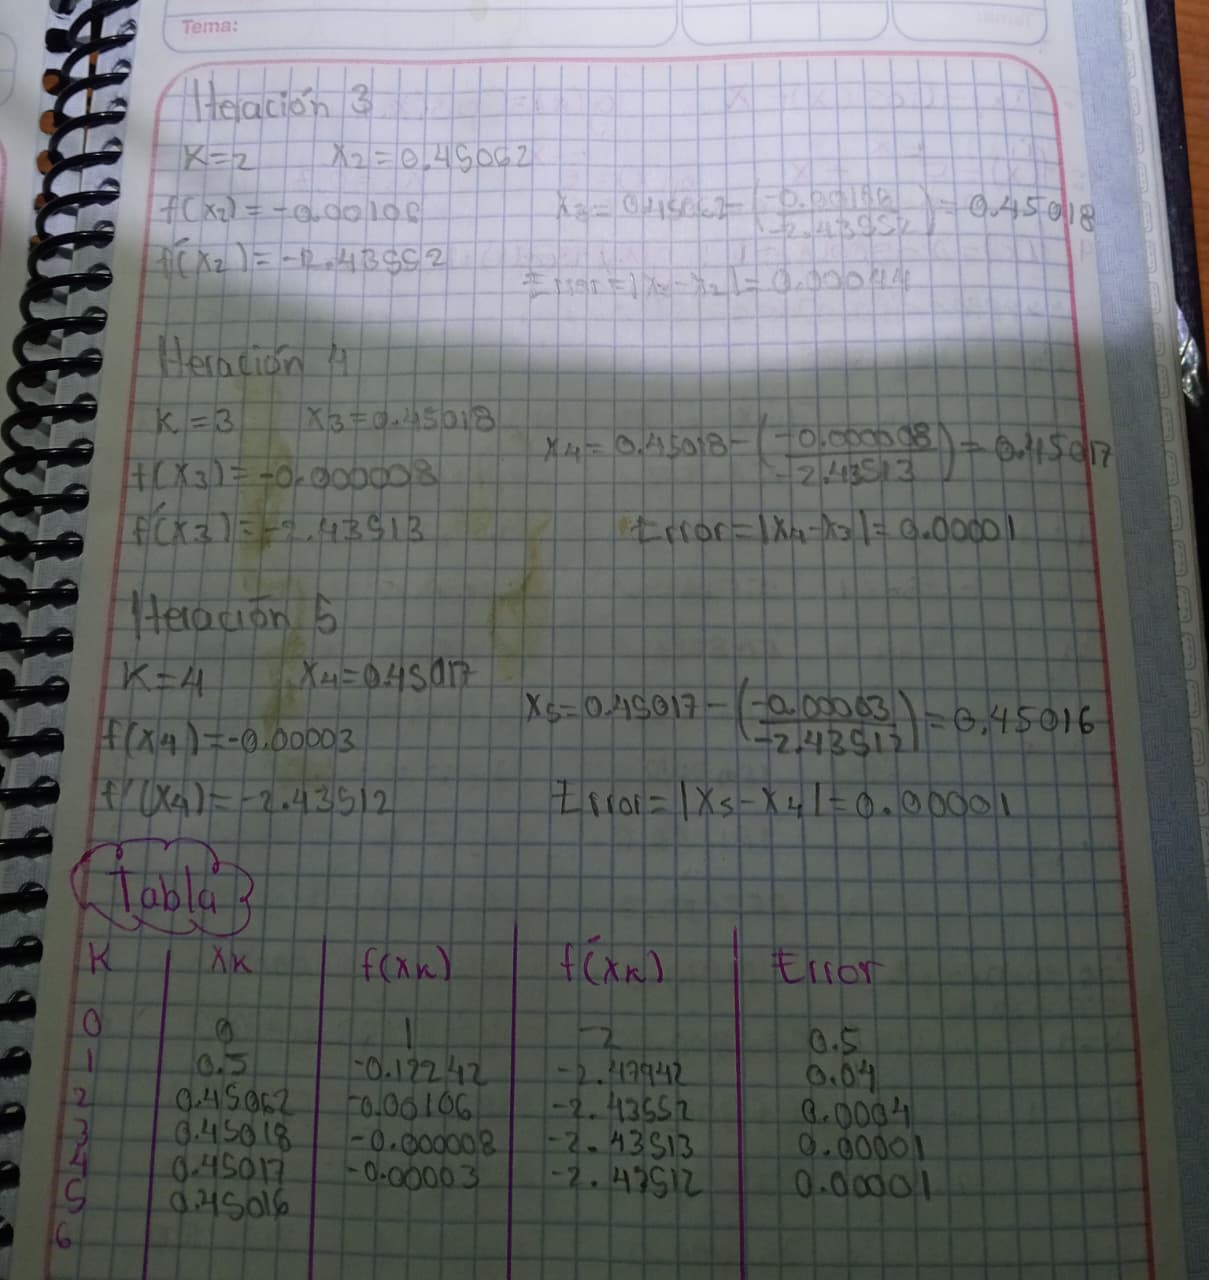
\includegraphics[width=2.60417in,height=\textheight,keepaspectratio,alt={pag.1}]{Newton _5.jpg}

\subsection{\texorpdfstring{\emph{Ejercicios en código
}}{Ejercicios en código }}\label{ejercicios-en-cuxf3digo-2}

\begin{Shaded}
\begin{Highlighting}[]
\NormalTok{newton\_completo }\OtherTok{\textless{}{-}} \ControlFlowTok{function}\NormalTok{(f, df, x0, }\AttributeTok{tol =} \FloatTok{1e{-}6}\NormalTok{, }\AttributeTok{iter\_max =} \DecValTok{10}\NormalTok{, }\AttributeTok{nombre\_funcion =} \StringTok{"f(x)"}\NormalTok{, }\AttributeTok{nombre\_latex =} \StringTok{"f(x)"}\NormalTok{) \{}
  
\NormalTok{  iter }\OtherTok{\textless{}{-}} \DecValTok{0}
\NormalTok{  error }\OtherTok{\textless{}{-}} \DecValTok{1}
\NormalTok{  x\_actual }\OtherTok{\textless{}{-}}\NormalTok{ x0}
  
  \CommentTok{\# Crear dataframe para almacenar resultados}
\NormalTok{  resultado }\OtherTok{\textless{}{-}} \FunctionTok{data.frame}\NormalTok{(}
    \AttributeTok{k =} \DecValTok{1}\SpecialCharTok{:}\NormalTok{iter\_max,}
    \AttributeTok{x\_k =} \FunctionTok{numeric}\NormalTok{(iter\_max),}
    \AttributeTok{f\_xk =} \FunctionTok{numeric}\NormalTok{(iter\_max),}
    \AttributeTok{df\_xk =} \FunctionTok{numeric}\NormalTok{(iter\_max),}
    \AttributeTok{error =} \FunctionTok{numeric}\NormalTok{(iter\_max),}
    \AttributeTok{stringsAsFactors =} \ConstantTok{FALSE}
\NormalTok{  )}
  
\NormalTok{  puntos\_x }\OtherTok{\textless{}{-}} \FunctionTok{numeric}\NormalTok{(iter\_max }\SpecialCharTok{+} \DecValTok{1}\NormalTok{)}
\NormalTok{  puntos\_x[}\DecValTok{1}\NormalTok{] }\OtherTok{\textless{}{-}}\NormalTok{ x0}
  
  \CommentTok{\# Iteraciones del método de Newton}
  \ControlFlowTok{for}\NormalTok{ (k }\ControlFlowTok{in} \DecValTok{1}\SpecialCharTok{:}\NormalTok{iter\_max) \{}
\NormalTok{    x\_siguiente }\OtherTok{\textless{}{-}}\NormalTok{ x\_actual }\SpecialCharTok{{-}} \FunctionTok{f}\NormalTok{(x\_actual)}\SpecialCharTok{/}\FunctionTok{df}\NormalTok{(x\_actual)}
\NormalTok{    error }\OtherTok{\textless{}{-}} \FunctionTok{abs}\NormalTok{(x\_siguiente }\SpecialCharTok{{-}}\NormalTok{ x\_actual)}
    
\NormalTok{    resultado[k, }\DecValTok{2}\SpecialCharTok{:}\DecValTok{5}\NormalTok{] }\OtherTok{\textless{}{-}} \FunctionTok{list}\NormalTok{(x\_actual, }\FunctionTok{f}\NormalTok{(x\_actual), }\FunctionTok{df}\NormalTok{(x\_actual), error)}
\NormalTok{    puntos\_x[k }\SpecialCharTok{+} \DecValTok{1}\NormalTok{] }\OtherTok{\textless{}{-}}\NormalTok{ x\_siguiente}
\NormalTok{    x\_actual }\OtherTok{\textless{}{-}}\NormalTok{ x\_siguiente}
    
    \ControlFlowTok{if}\NormalTok{ (error }\SpecialCharTok{\textless{}}\NormalTok{ tol) \{}
\NormalTok{      resultado }\OtherTok{\textless{}{-}}\NormalTok{ resultado[}\DecValTok{1}\SpecialCharTok{:}\NormalTok{k, ]}
\NormalTok{      puntos\_x }\OtherTok{\textless{}{-}}\NormalTok{ puntos\_x[}\DecValTok{1}\SpecialCharTok{:}\NormalTok{(k }\SpecialCharTok{+} \DecValTok{1}\NormalTok{)]}
      \ControlFlowTok{break}
\NormalTok{    \}}
\NormalTok{  \}}
  
  \FunctionTok{return}\NormalTok{(}\FunctionTok{list}\NormalTok{(}\AttributeTok{raiz =}\NormalTok{ x\_actual, }\AttributeTok{tabla =}\NormalTok{ resultado, }\AttributeTok{puntos =}\NormalTok{ puntos\_x))}
\NormalTok{\}}

\NormalTok{crear\_grafica\_newton }\OtherTok{\textless{}{-}} \ControlFlowTok{function}\NormalTok{(f, puntos\_x, nombre\_latex) \{}
\NormalTok{  x\_min }\OtherTok{\textless{}{-}} \FunctionTok{min}\NormalTok{(puntos\_x) }\SpecialCharTok{{-}} \FloatTok{0.5}
\NormalTok{  x\_max }\OtherTok{\textless{}{-}} \FunctionTok{max}\NormalTok{(puntos\_x) }\SpecialCharTok{+} \FloatTok{0.5}
\NormalTok{  x\_vals }\OtherTok{\textless{}{-}} \FunctionTok{seq}\NormalTok{(x\_min, x\_max, }\AttributeTok{length.out =} \DecValTok{400}\NormalTok{)}
\NormalTok{  y\_vals }\OtherTok{\textless{}{-}} \FunctionTok{sapply}\NormalTok{(x\_vals, f)}
  
  \FunctionTok{plot}\NormalTok{(x\_vals, y\_vals, }\AttributeTok{type =} \StringTok{"l"}\NormalTok{, }\AttributeTok{lwd =} \DecValTok{3}\NormalTok{, }\AttributeTok{col =} \StringTok{"blue"}\NormalTok{,}
       \AttributeTok{main =} \FunctionTok{paste}\NormalTok{(}\StringTok{"Método de Newton para"}\NormalTok{, nombre\_latex),}
       \AttributeTok{xlab =} \StringTok{"x"}\NormalTok{, }\AttributeTok{ylab =} \StringTok{"f(x)"}\NormalTok{,}
       \AttributeTok{ylim =} \FunctionTok{range}\NormalTok{(y\_vals))}
  
  \FunctionTok{abline}\NormalTok{(}\AttributeTok{h =} \DecValTok{0}\NormalTok{, }\AttributeTok{col =} \StringTok{"red"}\NormalTok{, }\AttributeTok{lty =} \DecValTok{2}\NormalTok{, }\AttributeTok{lwd =} \DecValTok{1}\NormalTok{)}
  
\NormalTok{  n\_puntos }\OtherTok{\textless{}{-}} \FunctionTok{length}\NormalTok{(puntos\_x)}
\NormalTok{  colores }\OtherTok{\textless{}{-}} \FunctionTok{rainbow}\NormalTok{(n\_puntos)}
  
  \ControlFlowTok{for}\NormalTok{ (i }\ControlFlowTok{in} \DecValTok{1}\SpecialCharTok{:}\NormalTok{n\_puntos) \{}
\NormalTok{    x\_point }\OtherTok{\textless{}{-}}\NormalTok{ puntos\_x[i]}
\NormalTok{    y\_point }\OtherTok{\textless{}{-}} \FunctionTok{f}\NormalTok{(x\_point)}
    
    \FunctionTok{points}\NormalTok{(x\_point, y\_point, }\AttributeTok{col =}\NormalTok{ colores[i], }\AttributeTok{pch =} \DecValTok{19}\NormalTok{, }\AttributeTok{cex =} \FloatTok{1.2}\NormalTok{)}
    \FunctionTok{segments}\NormalTok{(x\_point, y\_point, x\_point, }\DecValTok{0}\NormalTok{, }\AttributeTok{col =}\NormalTok{ colores[i], }\AttributeTok{lty =} \DecValTok{3}\NormalTok{, }\AttributeTok{lwd =} \DecValTok{1}\NormalTok{)}
    \FunctionTok{points}\NormalTok{(x\_point, }\DecValTok{0}\NormalTok{, }\AttributeTok{col =}\NormalTok{ colores[i], }\AttributeTok{pch =} \DecValTok{4}\NormalTok{, }\AttributeTok{cex =} \FloatTok{1.5}\NormalTok{, }\AttributeTok{lwd =} \DecValTok{2}\NormalTok{)}
    
    \ControlFlowTok{if}\NormalTok{ (i }\SpecialCharTok{\%\%} \DecValTok{2} \SpecialCharTok{==} \DecValTok{0} \SpecialCharTok{||}\NormalTok{ i }\SpecialCharTok{==}\NormalTok{ n\_puntos) \{}
      \FunctionTok{text}\NormalTok{(x\_point, }\FunctionTok{ifelse}\NormalTok{(y\_point }\SpecialCharTok{\textgreater{}=} \DecValTok{0}\NormalTok{, y\_point }\SpecialCharTok{+} \FloatTok{0.1}\NormalTok{, y\_point }\SpecialCharTok{{-}} \FloatTok{0.1}\NormalTok{), }
           \AttributeTok{labels =}\NormalTok{ i, }\AttributeTok{col =}\NormalTok{ colores[i], }\AttributeTok{font =} \DecValTok{2}\NormalTok{, }\AttributeTok{cex =} \FloatTok{0.8}\NormalTok{)}
\NormalTok{    \}}
\NormalTok{  \}}
  
\NormalTok{  raiz\_final }\OtherTok{\textless{}{-}}\NormalTok{ puntos\_x[n\_puntos]}
  \FunctionTok{points}\NormalTok{(raiz\_final, }\DecValTok{0}\NormalTok{, }\AttributeTok{col =} \StringTok{"darkred"}\NormalTok{, }\AttributeTok{pch =} \DecValTok{17}\NormalTok{, }\AttributeTok{cex =} \DecValTok{2}\NormalTok{, }\AttributeTok{lwd =} \DecValTok{2}\NormalTok{)}
  \FunctionTok{text}\NormalTok{(raiz\_final, }\SpecialCharTok{{-}}\FloatTok{0.2}\NormalTok{, }\AttributeTok{labels =} \FunctionTok{paste}\NormalTok{(}\StringTok{"Raíz ≈"}\NormalTok{, }\FunctionTok{round}\NormalTok{(raiz\_final, }\DecValTok{6}\NormalTok{)), }
       \AttributeTok{col =} \StringTok{"darkred"}\NormalTok{, }\AttributeTok{font =} \DecValTok{2}\NormalTok{)}
  
  \FunctionTok{legend}\NormalTok{(}\StringTok{"topright"}\NormalTok{, }
         \AttributeTok{legend =} \FunctionTok{c}\NormalTok{(}\StringTok{"f(x)"}\NormalTok{, }\StringTok{"Eje x"}\NormalTok{, }\StringTok{"Puntos iteración"}\NormalTok{, }\StringTok{"Proyecciones"}\NormalTok{, }\StringTok{"Raíz final"}\NormalTok{),}
         \AttributeTok{col =} \FunctionTok{c}\NormalTok{(}\StringTok{"blue"}\NormalTok{, }\StringTok{"red"}\NormalTok{, }\StringTok{"purple"}\NormalTok{, }\StringTok{"green"}\NormalTok{, }\StringTok{"darkred"}\NormalTok{),}
         \AttributeTok{lty =} \FunctionTok{c}\NormalTok{(}\DecValTok{1}\NormalTok{, }\DecValTok{2}\NormalTok{, }\ConstantTok{NA}\NormalTok{, }\DecValTok{3}\NormalTok{, }\ConstantTok{NA}\NormalTok{), }
         \AttributeTok{pch =} \FunctionTok{c}\NormalTok{(}\ConstantTok{NA}\NormalTok{, }\ConstantTok{NA}\NormalTok{, }\DecValTok{19}\NormalTok{, }\ConstantTok{NA}\NormalTok{, }\DecValTok{17}\NormalTok{),}
         \AttributeTok{lwd =} \FunctionTok{c}\NormalTok{(}\DecValTok{3}\NormalTok{, }\DecValTok{1}\NormalTok{, }\ConstantTok{NA}\NormalTok{, }\DecValTok{1}\NormalTok{, }\DecValTok{2}\NormalTok{))}
\NormalTok{\}}
\end{Highlighting}
\end{Shaded}

\subsubsection{3:}\label{section-42}

\(f(x) = x^4 - 3x^3 + 2\) , \([a,b]\) = \([1.5,2]\)

\begin{Shaded}
\begin{Highlighting}[]
\NormalTok{f3 }\OtherTok{\textless{}{-}} \ControlFlowTok{function}\NormalTok{(x) x}\SpecialCharTok{\^{}}\DecValTok{4} \SpecialCharTok{{-}} \DecValTok{3}\SpecialCharTok{*}\NormalTok{x}\SpecialCharTok{\^{}}\DecValTok{3} \SpecialCharTok{+} \DecValTok{2}
\NormalTok{df3 }\OtherTok{\textless{}{-}} \ControlFlowTok{function}\NormalTok{(x) }\DecValTok{4}\SpecialCharTok{*}\NormalTok{x}\SpecialCharTok{\^{}}\DecValTok{3} \SpecialCharTok{{-}} \DecValTok{9}\SpecialCharTok{*}\NormalTok{x}\SpecialCharTok{\^{}}\DecValTok{2}

\NormalTok{resultado\_newton3 }\OtherTok{\textless{}{-}} \FunctionTok{newton\_completo}\NormalTok{(f3, df3, }\AttributeTok{x0 =} \FloatTok{1.5}\NormalTok{, }\AttributeTok{iter\_max =} \DecValTok{10}\NormalTok{)}

\NormalTok{knitr}\SpecialCharTok{::}\FunctionTok{kable}\NormalTok{(resultado\_newton3}\SpecialCharTok{$}\NormalTok{tabla, }\AttributeTok{digits =} \DecValTok{6}\NormalTok{,}
             \AttributeTok{caption =} \StringTok{"Iteraciones del método de Newton para $f(x) = x\^{}4 {-} 3x\^{}3 + 2$"}\NormalTok{)}
\end{Highlighting}
\end{Shaded}

\begin{longtable}[]{@{}rrrrr@{}}
\caption{Iteraciones del método de Newton para
\(f(x) = x^4 - 3x^3 + 2\)}\tabularnewline
\toprule\noalign{}
k & x\_k & f\_xk & df\_xk & error \\
\midrule\noalign{}
\endfirsthead
\toprule\noalign{}
k & x\_k & f\_xk & df\_xk & error \\
\midrule\noalign{}
\endhead
\bottomrule\noalign{}
\endlastfoot
1 & 1.500000 & -3.062500 & -6.750000 & 0.453704 \\
2 & 1.046296 & -0.237808 & -5.270951 & 0.045117 \\
3 & 1.001180 & -0.005902 & -5.007074 & 0.001179 \\
4 & 1.000001 & -0.000004 & -5.000005 & 0.000001 \\
\end{longtable}

\begin{Shaded}
\begin{Highlighting}[]
\FunctionTok{cat}\NormalTok{(}\StringTok{"Raíz aproximada:"}\NormalTok{, }\FunctionTok{round}\NormalTok{(resultado\_newton3}\SpecialCharTok{$}\NormalTok{raiz, }\DecValTok{8}\NormalTok{), }\StringTok{"}\SpecialCharTok{\textbackslash{}n}\StringTok{"}\NormalTok{)}
\end{Highlighting}
\end{Shaded}

\begin{verbatim}
## Raíz aproximada: 1
\end{verbatim}

\begin{Shaded}
\begin{Highlighting}[]
\FunctionTok{cat}\NormalTok{(}\StringTok{"Iteraciones realizadas:"}\NormalTok{, }\FunctionTok{nrow}\NormalTok{(resultado\_newton3}\SpecialCharTok{$}\NormalTok{tabla), }\StringTok{"}\SpecialCharTok{\textbackslash{}n}\StringTok{"}\NormalTok{)}
\end{Highlighting}
\end{Shaded}

\begin{verbatim}
## Iteraciones realizadas: 4
\end{verbatim}

\begin{Shaded}
\begin{Highlighting}[]
\FunctionTok{cat}\NormalTok{(}\StringTok{"Error final:"}\NormalTok{, resultado\_newton3}\SpecialCharTok{$}\NormalTok{tabla}\SpecialCharTok{$}\NormalTok{error[}\FunctionTok{nrow}\NormalTok{(resultado\_newton3}\SpecialCharTok{$}\NormalTok{tabla)], }\StringTok{"}\SpecialCharTok{\textbackslash{}n}\StringTok{"}\NormalTok{)}
\end{Highlighting}
\end{Shaded}

\begin{verbatim}
## Error final: 8.330873e-07
\end{verbatim}

\begin{Shaded}
\begin{Highlighting}[]
\FunctionTok{crear\_grafica\_newton}\NormalTok{(f3, resultado\_newton3}\SpecialCharTok{$}\NormalTok{puntos, }\StringTok{"$f(x) = x\^{}4 {-} 3x\^{}3 + 2$"}\NormalTok{)}
\end{Highlighting}
\end{Shaded}

\pandocbounded{\includegraphics[keepaspectratio]{Notas_MN_LILIANA_CS_files/figure-latex/unnamed-chunk-466-1.pdf}}

\subsubsection{4:}\label{section-43}

\(f(x) = sin(x) - x/3\) , \([a,b] = [0,2]\)

\begin{Shaded}
\begin{Highlighting}[]
\NormalTok{f4 }\OtherTok{\textless{}{-}} \ControlFlowTok{function}\NormalTok{(x) }\FunctionTok{sin}\NormalTok{(x) }\SpecialCharTok{{-}}\NormalTok{ x}\SpecialCharTok{/}\DecValTok{3}
\NormalTok{df4 }\OtherTok{\textless{}{-}} \ControlFlowTok{function}\NormalTok{(x) }\FunctionTok{cos}\NormalTok{(x) }\SpecialCharTok{{-}} \DecValTok{1}\SpecialCharTok{/}\DecValTok{3}

\NormalTok{resultado\_newton4 }\OtherTok{\textless{}{-}} \FunctionTok{newton\_completo}\NormalTok{(f4, df4, }\AttributeTok{x0 =} \DecValTok{2}\NormalTok{, }\AttributeTok{iter\_max =} \DecValTok{10}\NormalTok{)}

\NormalTok{knitr}\SpecialCharTok{::}\FunctionTok{kable}\NormalTok{(resultado\_newton4}\SpecialCharTok{$}\NormalTok{tabla, }\AttributeTok{digits =} \DecValTok{6}\NormalTok{,}
             \AttributeTok{caption =} \StringTok{"Iteraciones del método de Newton para $f(x) = }\SpecialCharTok{\textbackslash{}\textbackslash{}}\StringTok{sin(x) {-} }\SpecialCharTok{\textbackslash{}\textbackslash{}}\StringTok{frac\{x\}\{3\}$"}\NormalTok{)}
\end{Highlighting}
\end{Shaded}

\begin{longtable}[]{@{}rrrrr@{}}
\caption{Iteraciones del método de Newton para
\(f(x) = \sin(x) - \frac{x}{3}\)}\tabularnewline
\toprule\noalign{}
k & x\_k & f\_xk & df\_xk & error \\
\midrule\noalign{}
\endfirsthead
\toprule\noalign{}
k & x\_k & f\_xk & df\_xk & error \\
\midrule\noalign{}
\endhead
\bottomrule\noalign{}
\endlastfoot
1 & 2.000000 & 0.242631 & -0.749480 & 0.323732 \\
2 & 2.323732 & -0.044893 & -1.017117 & 0.044137 \\
3 & 2.279595 & -0.000720 & -0.984255 & 0.000732 \\
4 & 2.278863 & 0.000000 & -0.983700 & 0.000000 \\
\end{longtable}

\begin{Shaded}
\begin{Highlighting}[]
\FunctionTok{cat}\NormalTok{(}\StringTok{"Raíz aproximada:"}\NormalTok{, }\FunctionTok{round}\NormalTok{(resultado\_newton4}\SpecialCharTok{$}\NormalTok{raiz, }\DecValTok{8}\NormalTok{), }\StringTok{"}\SpecialCharTok{\textbackslash{}n}\StringTok{"}\NormalTok{)}
\end{Highlighting}
\end{Shaded}

\begin{verbatim}
## Raíz aproximada: 2.278863
\end{verbatim}

\begin{Shaded}
\begin{Highlighting}[]
\FunctionTok{cat}\NormalTok{(}\StringTok{"Iteraciones realizadas:"}\NormalTok{, }\FunctionTok{nrow}\NormalTok{(resultado\_newton4}\SpecialCharTok{$}\NormalTok{tabla), }\StringTok{"}\SpecialCharTok{\textbackslash{}n}\StringTok{"}\NormalTok{)}
\end{Highlighting}
\end{Shaded}

\begin{verbatim}
## Iteraciones realizadas: 4
\end{verbatim}

\begin{Shaded}
\begin{Highlighting}[]
\FunctionTok{cat}\NormalTok{(}\StringTok{"Error final:"}\NormalTok{, resultado\_newton4}\SpecialCharTok{$}\NormalTok{tabla}\SpecialCharTok{$}\NormalTok{error[}\FunctionTok{nrow}\NormalTok{(resultado\_newton4}\SpecialCharTok{$}\NormalTok{tabla)], }\StringTok{"}\SpecialCharTok{\textbackslash{}n}\StringTok{"}\NormalTok{)}
\end{Highlighting}
\end{Shaded}

\begin{verbatim}
## Error final: 2.067718e-07
\end{verbatim}

\begin{Shaded}
\begin{Highlighting}[]
\FunctionTok{crear\_grafica\_newton}\NormalTok{(f4, resultado\_newton4}\SpecialCharTok{$}\NormalTok{puntos, }\StringTok{"$f(x) = }\SpecialCharTok{\textbackslash{}\textbackslash{}}\StringTok{sin(x) {-} }\SpecialCharTok{\textbackslash{}\textbackslash{}}\StringTok{frac\{x\}\{3\}$"}\NormalTok{)}
\end{Highlighting}
\end{Shaded}

\pandocbounded{\includegraphics[keepaspectratio]{Notas_MN_LILIANA_CS_files/figure-latex/unnamed-chunk-469-1.pdf}}

\subsubsection{5:}\label{section-44}

\(f(x) = e^{-x} - x\) , \([a,b] = [0,1]\)

\begin{Shaded}
\begin{Highlighting}[]
\NormalTok{f5 }\OtherTok{\textless{}{-}} \ControlFlowTok{function}\NormalTok{(x) }\FunctionTok{exp}\NormalTok{(}\SpecialCharTok{{-}}\NormalTok{x) }\SpecialCharTok{{-}}\NormalTok{ x}
\NormalTok{df5 }\OtherTok{\textless{}{-}} \ControlFlowTok{function}\NormalTok{(x) }\SpecialCharTok{{-}}\FunctionTok{exp}\NormalTok{(}\SpecialCharTok{{-}}\NormalTok{x) }\SpecialCharTok{{-}} \DecValTok{1}

\NormalTok{resultado\_newton5 }\OtherTok{\textless{}{-}} \FunctionTok{newton\_completo}\NormalTok{(f5, df5, }\AttributeTok{x0 =} \FloatTok{0.5}\NormalTok{, }\AttributeTok{iter\_max =} \DecValTok{10}\NormalTok{)}

\NormalTok{knitr}\SpecialCharTok{::}\FunctionTok{kable}\NormalTok{(resultado\_newton5}\SpecialCharTok{$}\NormalTok{tabla, }\AttributeTok{digits =} \DecValTok{6}\NormalTok{,}
             \AttributeTok{caption =} \StringTok{"Iteraciones del método de Newton para $f(x) = e\^{}\{{-}x\} {-} x$"}\NormalTok{)}
\end{Highlighting}
\end{Shaded}

\begin{longtable}[]{@{}rrrrr@{}}
\caption{Iteraciones del método de Newton para
\(f(x) = e^{-x} - x\)}\tabularnewline
\toprule\noalign{}
k & x\_k & f\_xk & df\_xk & error \\
\midrule\noalign{}
\endfirsthead
\toprule\noalign{}
k & x\_k & f\_xk & df\_xk & error \\
\midrule\noalign{}
\endhead
\bottomrule\noalign{}
\endlastfoot
1 & 0.500000 & 0.106531 & -1.606531 & 0.066311 \\
2 & 0.566311 & 0.001305 & -1.567616 & 0.000832 \\
3 & 0.567143 & 0.000000 & -1.567143 & 0.000000 \\
\end{longtable}

\begin{Shaded}
\begin{Highlighting}[]
\FunctionTok{cat}\NormalTok{(}\StringTok{"Raíz aproximada:"}\NormalTok{, }\FunctionTok{round}\NormalTok{(resultado\_newton5}\SpecialCharTok{$}\NormalTok{raiz, }\DecValTok{8}\NormalTok{), }\StringTok{"}\SpecialCharTok{\textbackslash{}n}\StringTok{"}\NormalTok{)}
\end{Highlighting}
\end{Shaded}

\begin{verbatim}
## Raíz aproximada: 0.5671433
\end{verbatim}

\begin{Shaded}
\begin{Highlighting}[]
\FunctionTok{cat}\NormalTok{(}\StringTok{"Iteraciones realizadas:"}\NormalTok{, }\FunctionTok{nrow}\NormalTok{(resultado\_newton5}\SpecialCharTok{$}\NormalTok{tabla), }\StringTok{"}\SpecialCharTok{\textbackslash{}n}\StringTok{"}\NormalTok{)}
\end{Highlighting}
\end{Shaded}

\begin{verbatim}
## Iteraciones realizadas: 3
\end{verbatim}

\begin{Shaded}
\begin{Highlighting}[]
\FunctionTok{cat}\NormalTok{(}\StringTok{"Error final:"}\NormalTok{, resultado\_newton5}\SpecialCharTok{$}\NormalTok{tabla}\SpecialCharTok{$}\NormalTok{error[}\FunctionTok{nrow}\NormalTok{(resultado\_newton5}\SpecialCharTok{$}\NormalTok{tabla)], }\StringTok{"}\SpecialCharTok{\textbackslash{}n}\StringTok{"}\NormalTok{)}
\end{Highlighting}
\end{Shaded}

\begin{verbatim}
## Error final: 1.253749e-07
\end{verbatim}

\begin{Shaded}
\begin{Highlighting}[]
\FunctionTok{crear\_grafica\_newton}\NormalTok{(f5, resultado\_newton5}\SpecialCharTok{$}\NormalTok{puntos, }\StringTok{"$f(x) = e\^{}\{{-}x\} {-} x$"}\NormalTok{)}
\end{Highlighting}
\end{Shaded}

\pandocbounded{\includegraphics[keepaspectratio]{Notas_MN_LILIANA_CS_files/figure-latex/unnamed-chunk-472-1.pdf}}

\subsubsection{6:}\label{section-45}

\(f(x) = x^3 - 2x - 5\) , \([a,b] = [2,3]\)

\begin{Shaded}
\begin{Highlighting}[]
\NormalTok{f6 }\OtherTok{\textless{}{-}} \ControlFlowTok{function}\NormalTok{(x) x}\SpecialCharTok{\^{}}\DecValTok{3} \SpecialCharTok{{-}} \DecValTok{2}\SpecialCharTok{*}\NormalTok{x }\SpecialCharTok{{-}} \DecValTok{5}
\NormalTok{df6 }\OtherTok{\textless{}{-}} \ControlFlowTok{function}\NormalTok{(x) }\DecValTok{3}\SpecialCharTok{*}\NormalTok{x}\SpecialCharTok{\^{}}\DecValTok{2} \SpecialCharTok{{-}} \DecValTok{2}

\NormalTok{resultado\_newton6 }\OtherTok{\textless{}{-}} \FunctionTok{newton\_completo}\NormalTok{(f6, df6, }\AttributeTok{x0 =} \FloatTok{2.5}\NormalTok{, }\AttributeTok{iter\_max =} \DecValTok{10}\NormalTok{)}

\NormalTok{knitr}\SpecialCharTok{::}\FunctionTok{kable}\NormalTok{(resultado\_newton6}\SpecialCharTok{$}\NormalTok{tabla, }\AttributeTok{digits =} \DecValTok{6}\NormalTok{,}
             \AttributeTok{caption =} \StringTok{"Iteraciones del método de Newton para $f(x) = x\^{}3 {-} 2x {-} 5$"}\NormalTok{)}
\end{Highlighting}
\end{Shaded}

\begin{longtable}[]{@{}rrrrr@{}}
\caption{Iteraciones del método de Newton para
\(f(x) = x^3 - 2x - 5\)}\tabularnewline
\toprule\noalign{}
k & x\_k & f\_xk & df\_xk & error \\
\midrule\noalign{}
\endfirsthead
\toprule\noalign{}
k & x\_k & f\_xk & df\_xk & error \\
\midrule\noalign{}
\endhead
\bottomrule\noalign{}
\endlastfoot
1 & 2.500000 & 5.625000 & 16.75000 & 0.335821 \\
2 & 2.164179 & 0.807945 & 12.05101 & 0.067044 \\
3 & 2.097135 & 0.028882 & 11.19393 & 0.002580 \\
4 & 2.094555 & 0.000042 & 11.16149 & 0.000004 \\
5 & 2.094551 & 0.000000 & 11.16144 & 0.000000 \\
\end{longtable}

\begin{Shaded}
\begin{Highlighting}[]
\FunctionTok{cat}\NormalTok{(}\StringTok{"Raíz aproximada:"}\NormalTok{, }\FunctionTok{round}\NormalTok{(resultado\_newton6}\SpecialCharTok{$}\NormalTok{raiz, }\DecValTok{8}\NormalTok{), }\StringTok{"}\SpecialCharTok{\textbackslash{}n}\StringTok{"}\NormalTok{)}
\end{Highlighting}
\end{Shaded}

\begin{verbatim}
## Raíz aproximada: 2.094551
\end{verbatim}

\begin{Shaded}
\begin{Highlighting}[]
\FunctionTok{cat}\NormalTok{(}\StringTok{"Iteraciones realizadas:"}\NormalTok{, }\FunctionTok{nrow}\NormalTok{(resultado\_newton6}\SpecialCharTok{$}\NormalTok{tabla), }\StringTok{"}\SpecialCharTok{\textbackslash{}n}\StringTok{"}\NormalTok{)}
\end{Highlighting}
\end{Shaded}

\begin{verbatim}
## Iteraciones realizadas: 5
\end{verbatim}

\begin{Shaded}
\begin{Highlighting}[]
\FunctionTok{cat}\NormalTok{(}\StringTok{"Error final:"}\NormalTok{, resultado\_newton6}\SpecialCharTok{$}\NormalTok{tabla}\SpecialCharTok{$}\NormalTok{error[}\FunctionTok{nrow}\NormalTok{(resultado\_newton6}\SpecialCharTok{$}\NormalTok{tabla)], }\StringTok{"}\SpecialCharTok{\textbackslash{}n}\StringTok{"}\NormalTok{)}
\end{Highlighting}
\end{Shaded}

\begin{verbatim}
## Error final: 7.920331e-12
\end{verbatim}

\begin{Shaded}
\begin{Highlighting}[]
\FunctionTok{crear\_grafica\_newton}\NormalTok{(f6, resultado\_newton6}\SpecialCharTok{$}\NormalTok{puntos, }\StringTok{"$f(x) = x\^{}3 {-} 2x {-} 5$"}\NormalTok{)}
\end{Highlighting}
\end{Shaded}

\pandocbounded{\includegraphics[keepaspectratio]{Notas_MN_LILIANA_CS_files/figure-latex/unnamed-chunk-475-1.pdf}}

\subsubsection{7:}\label{section-46}

\(f(x) = x^5 - 3x + 1\) , \([a,b] = [0,1]\)

\begin{Shaded}
\begin{Highlighting}[]
\NormalTok{f7 }\OtherTok{\textless{}{-}} \ControlFlowTok{function}\NormalTok{(x) x}\SpecialCharTok{\^{}}\DecValTok{5} \SpecialCharTok{{-}} \DecValTok{3}\SpecialCharTok{*}\NormalTok{x }\SpecialCharTok{+} \DecValTok{1}
\NormalTok{df7 }\OtherTok{\textless{}{-}} \ControlFlowTok{function}\NormalTok{(x) }\DecValTok{5}\SpecialCharTok{*}\NormalTok{x}\SpecialCharTok{\^{}}\DecValTok{4} \SpecialCharTok{{-}} \DecValTok{3}

\NormalTok{resultado\_newton7 }\OtherTok{\textless{}{-}} \FunctionTok{newton\_completo}\NormalTok{(f7, df7, }\AttributeTok{x0 =} \FloatTok{0.5}\NormalTok{, }\AttributeTok{iter\_max =} \DecValTok{10}\NormalTok{)}

\NormalTok{knitr}\SpecialCharTok{::}\FunctionTok{kable}\NormalTok{(resultado\_newton7}\SpecialCharTok{$}\NormalTok{tabla, }\AttributeTok{digits =} \DecValTok{6}\NormalTok{,}
             \AttributeTok{caption =} \StringTok{"Iteraciones del método de Newton para $f(x) = x\^{}5 {-} 3x + 1$"}\NormalTok{)}
\end{Highlighting}
\end{Shaded}

\begin{longtable}[]{@{}rrrrr@{}}
\caption{Iteraciones del método de Newton para
\(f(x) = x^5 - 3x + 1\)}\tabularnewline
\toprule\noalign{}
k & x\_k & f\_xk & df\_xk & error \\
\midrule\noalign{}
\endfirsthead
\toprule\noalign{}
k & x\_k & f\_xk & df\_xk & error \\
\midrule\noalign{}
\endhead
\bottomrule\noalign{}
\endlastfoot
1 & 0.500000 & -0.468750 & -2.687500 & 0.174419 \\
2 & 0.325581 & 0.026914 & -2.943817 & 0.009143 \\
3 & 0.334724 & 0.000030 & -2.937235 & 0.000010 \\
4 & 0.334734 & 0.000000 & -2.937227 & 0.000000 \\
\end{longtable}

\begin{Shaded}
\begin{Highlighting}[]
\FunctionTok{cat}\NormalTok{(}\StringTok{"Raíz aproximada:"}\NormalTok{, }\FunctionTok{round}\NormalTok{(resultado\_newton7}\SpecialCharTok{$}\NormalTok{raiz, }\DecValTok{8}\NormalTok{), }\StringTok{"}\SpecialCharTok{\textbackslash{}n}\StringTok{"}\NormalTok{)}
\end{Highlighting}
\end{Shaded}

\begin{verbatim}
## Raíz aproximada: 0.3347341
\end{verbatim}

\begin{Shaded}
\begin{Highlighting}[]
\FunctionTok{cat}\NormalTok{(}\StringTok{"Iteraciones realizadas:"}\NormalTok{, }\FunctionTok{nrow}\NormalTok{(resultado\_newton7}\SpecialCharTok{$}\NormalTok{tabla), }\StringTok{"}\SpecialCharTok{\textbackslash{}n}\StringTok{"}\NormalTok{)}
\end{Highlighting}
\end{Shaded}

\begin{verbatim}
## Iteraciones realizadas: 4
\end{verbatim}

\begin{Shaded}
\begin{Highlighting}[]
\FunctionTok{cat}\NormalTok{(}\StringTok{"Error final:"}\NormalTok{, resultado\_newton7}\SpecialCharTok{$}\NormalTok{tabla}\SpecialCharTok{$}\NormalTok{error[}\FunctionTok{nrow}\NormalTok{(resultado\_newton7}\SpecialCharTok{$}\NormalTok{tabla)], }\StringTok{"}\SpecialCharTok{\textbackslash{}n}\StringTok{"}\NormalTok{)}
\end{Highlighting}
\end{Shaded}

\begin{verbatim}
## Error final: 1.302847e-11
\end{verbatim}

\begin{Shaded}
\begin{Highlighting}[]
\FunctionTok{crear\_grafica\_newton}\NormalTok{(f7, resultado\_newton7}\SpecialCharTok{$}\NormalTok{puntos, }\StringTok{"$f(x) = x\^{}5 {-} 3x + 1$"}\NormalTok{)}
\end{Highlighting}
\end{Shaded}

\pandocbounded{\includegraphics[keepaspectratio]{Notas_MN_LILIANA_CS_files/figure-latex/unnamed-chunk-478-1.pdf}}

\subsubsection{8:}\label{section-47}

\(f(x) = cos(x) - 2x\) , \([a,b] = [0,1]\)

\begin{Shaded}
\begin{Highlighting}[]
\NormalTok{f8 }\OtherTok{\textless{}{-}} \ControlFlowTok{function}\NormalTok{(x) }\FunctionTok{cos}\NormalTok{(x) }\SpecialCharTok{{-}} \DecValTok{2}\SpecialCharTok{*}\NormalTok{x}
\NormalTok{df8 }\OtherTok{\textless{}{-}} \ControlFlowTok{function}\NormalTok{(x) }\SpecialCharTok{{-}}\FunctionTok{sin}\NormalTok{(x) }\SpecialCharTok{{-}} \DecValTok{2}

\NormalTok{resultado\_newton8 }\OtherTok{\textless{}{-}} \FunctionTok{newton\_completo}\NormalTok{(f8, df8, }\AttributeTok{x0 =} \FloatTok{0.5}\NormalTok{, }\AttributeTok{iter\_max =} \DecValTok{10}\NormalTok{)}

\NormalTok{knitr}\SpecialCharTok{::}\FunctionTok{kable}\NormalTok{(resultado\_newton8}\SpecialCharTok{$}\NormalTok{tabla, }\AttributeTok{digits =} \DecValTok{6}\NormalTok{,}
             \AttributeTok{caption =} \StringTok{"Iteraciones del método de Newton para $f(x) = }\SpecialCharTok{\textbackslash{}\textbackslash{}}\StringTok{cos(x) {-} 2x$"}\NormalTok{)}
\end{Highlighting}
\end{Shaded}

\begin{longtable}[]{@{}rrrrr@{}}
\caption{Iteraciones del método de Newton para
\(f(x) = \cos(x) - 2x\)}\tabularnewline
\toprule\noalign{}
k & x\_k & f\_xk & df\_xk & error \\
\midrule\noalign{}
\endfirsthead
\toprule\noalign{}
k & x\_k & f\_xk & df\_xk & error \\
\midrule\noalign{}
\endhead
\bottomrule\noalign{}
\endlastfoot
1 & 0.500000 & -0.122417 & -2.479426 & 0.049373 \\
2 & 0.450627 & -0.001079 & -2.435530 & 0.000443 \\
3 & 0.450184 & 0.000000 & -2.435131 & 0.000000 \\
\end{longtable}

\begin{Shaded}
\begin{Highlighting}[]
\FunctionTok{cat}\NormalTok{(}\StringTok{"Raíz aproximada:"}\NormalTok{, }\FunctionTok{round}\NormalTok{(resultado\_newton8}\SpecialCharTok{$}\NormalTok{raiz, }\DecValTok{8}\NormalTok{), }\StringTok{"}\SpecialCharTok{\textbackslash{}n}\StringTok{"}\NormalTok{)}
\end{Highlighting}
\end{Shaded}

\begin{verbatim}
## Raíz aproximada: 0.4501836
\end{verbatim}

\begin{Shaded}
\begin{Highlighting}[]
\FunctionTok{cat}\NormalTok{(}\StringTok{"Iteraciones realizadas:"}\NormalTok{, }\FunctionTok{nrow}\NormalTok{(resultado\_newton8}\SpecialCharTok{$}\NormalTok{tabla), }\StringTok{"}\SpecialCharTok{\textbackslash{}n}\StringTok{"}\NormalTok{)}
\end{Highlighting}
\end{Shaded}

\begin{verbatim}
## Iteraciones realizadas: 3
\end{verbatim}

\begin{Shaded}
\begin{Highlighting}[]
\FunctionTok{cat}\NormalTok{(}\StringTok{"Error final:"}\NormalTok{, resultado\_newton8}\SpecialCharTok{$}\NormalTok{tabla}\SpecialCharTok{$}\NormalTok{error[}\FunctionTok{nrow}\NormalTok{(resultado\_newton8}\SpecialCharTok{$}\NormalTok{tabla)], }\StringTok{"}\SpecialCharTok{\textbackslash{}n}\StringTok{"}\NormalTok{)}
\end{Highlighting}
\end{Shaded}

\begin{verbatim}
## Error final: 3.62829e-08
\end{verbatim}

\begin{Shaded}
\begin{Highlighting}[]
\FunctionTok{crear\_grafica\_newton}\NormalTok{(f8, resultado\_newton8}\SpecialCharTok{$}\NormalTok{puntos, }\StringTok{"$f(x) = }\SpecialCharTok{\textbackslash{}\textbackslash{}}\StringTok{cos(x) {-} 2x$"}\NormalTok{)}
\end{Highlighting}
\end{Shaded}

\pandocbounded{\includegraphics[keepaspectratio]{Notas_MN_LILIANA_CS_files/figure-latex/unnamed-chunk-481-1.pdf}}

\subsubsection{9:}\label{section-48}

\(f(x) = ln(x + 2) + x - 1\) , \([a,b] = [0,1]\)

\begin{Shaded}
\begin{Highlighting}[]
\NormalTok{f9 }\OtherTok{\textless{}{-}} \ControlFlowTok{function}\NormalTok{(x) }\FunctionTok{log}\NormalTok{(x }\SpecialCharTok{+} \DecValTok{2}\NormalTok{) }\SpecialCharTok{+}\NormalTok{ x }\SpecialCharTok{{-}} \DecValTok{1}
\NormalTok{df9 }\OtherTok{\textless{}{-}} \ControlFlowTok{function}\NormalTok{(x) }\DecValTok{1}\SpecialCharTok{/}\NormalTok{(x }\SpecialCharTok{+} \DecValTok{2}\NormalTok{) }\SpecialCharTok{+} \DecValTok{1}

\NormalTok{resultado\_newton9 }\OtherTok{\textless{}{-}} \FunctionTok{newton\_completo}\NormalTok{(f9, df9, }\AttributeTok{x0 =} \DecValTok{0}\NormalTok{, }\AttributeTok{iter\_max =} \DecValTok{10}\NormalTok{)}

\NormalTok{knitr}\SpecialCharTok{::}\FunctionTok{kable}\NormalTok{(resultado\_newton9}\SpecialCharTok{$}\NormalTok{tabla, }\AttributeTok{digits =} \DecValTok{6}\NormalTok{,}
             \AttributeTok{caption =} \StringTok{"Iteraciones del método de Newton para $f(x) = }\SpecialCharTok{\textbackslash{}\textbackslash{}}\StringTok{ln(x + 2) + x {-} 1$"}\NormalTok{)}
\end{Highlighting}
\end{Shaded}

\begin{longtable}[]{@{}rrrrr@{}}
\caption{Iteraciones del método de Newton para
\(f(x) = \ln(x + 2) + x - 1\)}\tabularnewline
\toprule\noalign{}
k & x\_k & f\_xk & df\_xk & error \\
\midrule\noalign{}
\endfirsthead
\toprule\noalign{}
k & x\_k & f\_xk & df\_xk & error \\
\midrule\noalign{}
\endhead
\bottomrule\noalign{}
\endlastfoot
1 & 0.000000 & -0.306853 & 1.500000 & 0.204569 \\
2 & 0.204569 & -0.004900 & 1.453603 & 0.003371 \\
3 & 0.207939 & -0.000001 & 1.452911 & 0.000001 \\
\end{longtable}

\begin{Shaded}
\begin{Highlighting}[]
\FunctionTok{cat}\NormalTok{(}\StringTok{"Raíz aproximada:"}\NormalTok{, }\FunctionTok{round}\NormalTok{(resultado\_newton9}\SpecialCharTok{$}\NormalTok{raiz, }\DecValTok{8}\NormalTok{), }\StringTok{"}\SpecialCharTok{\textbackslash{}n}\StringTok{"}\NormalTok{)}
\end{Highlighting}
\end{Shaded}

\begin{verbatim}
## Raíz aproximada: 0.20794
\end{verbatim}

\begin{Shaded}
\begin{Highlighting}[]
\FunctionTok{cat}\NormalTok{(}\StringTok{"Iteraciones realizadas:"}\NormalTok{, }\FunctionTok{nrow}\NormalTok{(resultado\_newton9}\SpecialCharTok{$}\NormalTok{tabla), }\StringTok{"}\SpecialCharTok{\textbackslash{}n}\StringTok{"}\NormalTok{)}
\end{Highlighting}
\end{Shaded}

\begin{verbatim}
## Iteraciones realizadas: 3
\end{verbatim}

\begin{Shaded}
\begin{Highlighting}[]
\FunctionTok{cat}\NormalTok{(}\StringTok{"Error final:"}\NormalTok{, resultado\_newton9}\SpecialCharTok{$}\NormalTok{tabla}\SpecialCharTok{$}\NormalTok{error[}\FunctionTok{nrow}\NormalTok{(resultado\_newton9}\SpecialCharTok{$}\NormalTok{tabla)], }\StringTok{"}\SpecialCharTok{\textbackslash{}n}\StringTok{"}\NormalTok{)}
\end{Highlighting}
\end{Shaded}

\begin{verbatim}
## Error final: 8.036683e-07
\end{verbatim}

\begin{Shaded}
\begin{Highlighting}[]
\FunctionTok{crear\_grafica\_newton}\NormalTok{(f9, resultado\_newton9}\SpecialCharTok{$}\NormalTok{puntos, }\StringTok{"$f(x) = }\SpecialCharTok{\textbackslash{}\textbackslash{}}\StringTok{ln(x + 2) + x {-} 1$"}\NormalTok{)}
\end{Highlighting}
\end{Shaded}

\pandocbounded{\includegraphics[keepaspectratio]{Notas_MN_LILIANA_CS_files/figure-latex/unnamed-chunk-484-1.pdf}}

\subsubsection{11:}\label{section-49}

\(f(x) = x^3 - 4sin(x)\) , \([a,b] = [1,2]\)

\begin{Shaded}
\begin{Highlighting}[]
\NormalTok{f11 }\OtherTok{\textless{}{-}} \ControlFlowTok{function}\NormalTok{(x) x}\SpecialCharTok{\^{}}\DecValTok{3} \SpecialCharTok{{-}} \DecValTok{4}\SpecialCharTok{*}\FunctionTok{sin}\NormalTok{(x)}
\NormalTok{df11 }\OtherTok{\textless{}{-}} \ControlFlowTok{function}\NormalTok{(x) }\DecValTok{3}\SpecialCharTok{*}\NormalTok{x}\SpecialCharTok{\^{}}\DecValTok{2} \SpecialCharTok{{-}} \DecValTok{4}\SpecialCharTok{*}\FunctionTok{cos}\NormalTok{(x)}

\NormalTok{resultado\_newton11 }\OtherTok{\textless{}{-}} \FunctionTok{newton\_completo}\NormalTok{(f11, df11, }\AttributeTok{x0 =} \FloatTok{1.5}\NormalTok{, }\AttributeTok{iter\_max =} \DecValTok{10}\NormalTok{)}

\NormalTok{knitr}\SpecialCharTok{::}\FunctionTok{kable}\NormalTok{(resultado\_newton11}\SpecialCharTok{$}\NormalTok{tabla, }\AttributeTok{digits =} \DecValTok{6}\NormalTok{,}
             \AttributeTok{caption =} \StringTok{"Iteraciones del método de Newton para $f(x) = x\^{}3 {-} 4}\SpecialCharTok{\textbackslash{}\textbackslash{}}\StringTok{sin(x)$"}\NormalTok{)}
\end{Highlighting}
\end{Shaded}

\begin{longtable}[]{@{}rrrrr@{}}
\caption{Iteraciones del método de Newton para
\(f(x) = x^3 - 4\sin(x)\)}\tabularnewline
\toprule\noalign{}
k & x\_k & f\_xk & df\_xk & error \\
\midrule\noalign{}
\endfirsthead
\toprule\noalign{}
k & x\_k & f\_xk & df\_xk & error \\
\midrule\noalign{}
\endhead
\bottomrule\noalign{}
\endlastfoot
1 & 1.500000 & -0.614980 & 6.467051 & 0.095094 \\
2 & 1.595094 & 0.059621 & 7.730160 & 0.007713 \\
3 & 1.587382 & 0.000403 & 7.625679 & 0.000053 \\
4 & 1.587329 & 0.000000 & 7.624964 & 0.000000 \\
\end{longtable}

\begin{Shaded}
\begin{Highlighting}[]
\FunctionTok{cat}\NormalTok{(}\StringTok{"Raíz aproximada:"}\NormalTok{, }\FunctionTok{round}\NormalTok{(resultado\_newton11}\SpecialCharTok{$}\NormalTok{raiz, }\DecValTok{8}\NormalTok{), }\StringTok{"}\SpecialCharTok{\textbackslash{}n}\StringTok{"}\NormalTok{)}
\end{Highlighting}
\end{Shaded}

\begin{verbatim}
## Raíz aproximada: 1.587329
\end{verbatim}

\begin{Shaded}
\begin{Highlighting}[]
\FunctionTok{cat}\NormalTok{(}\StringTok{"Iteraciones realizadas:"}\NormalTok{, }\FunctionTok{nrow}\NormalTok{(resultado\_newton11}\SpecialCharTok{$}\NormalTok{tabla), }\StringTok{"}\SpecialCharTok{\textbackslash{}n}\StringTok{"}\NormalTok{)}
\end{Highlighting}
\end{Shaded}

\begin{verbatim}
## Iteraciones realizadas: 4
\end{verbatim}

\begin{Shaded}
\begin{Highlighting}[]
\FunctionTok{cat}\NormalTok{(}\StringTok{"Error final:"}\NormalTok{, resultado\_newton11}\SpecialCharTok{$}\NormalTok{tabla}\SpecialCharTok{$}\NormalTok{error[}\FunctionTok{nrow}\NormalTok{(resultado\_newton11}\SpecialCharTok{$}\NormalTok{tabla)], }\StringTok{"}\SpecialCharTok{\textbackslash{}n}\StringTok{"}\NormalTok{)}
\end{Highlighting}
\end{Shaded}

\begin{verbatim}
## Error final: 2.478495e-09
\end{verbatim}

\begin{Shaded}
\begin{Highlighting}[]
\FunctionTok{crear\_grafica\_newton}\NormalTok{(f11, resultado\_newton11}\SpecialCharTok{$}\NormalTok{puntos, }\StringTok{"$f(x) = x\^{}3 {-} 4}\SpecialCharTok{\textbackslash{}\textbackslash{}}\StringTok{sin(x)$"}\NormalTok{)}
\end{Highlighting}
\end{Shaded}

\pandocbounded{\includegraphics[keepaspectratio]{Notas_MN_LILIANA_CS_files/figure-latex/unnamed-chunk-487-1.pdf}}

\section{\texorpdfstring{\textbf{Método Punto
Fijo}}{Método Punto Fijo}}\label{muxe9todo-punto-fijo}

\subsection{\texorpdfstring{\emph{A mano}}{A mano}}\label{a-mano}

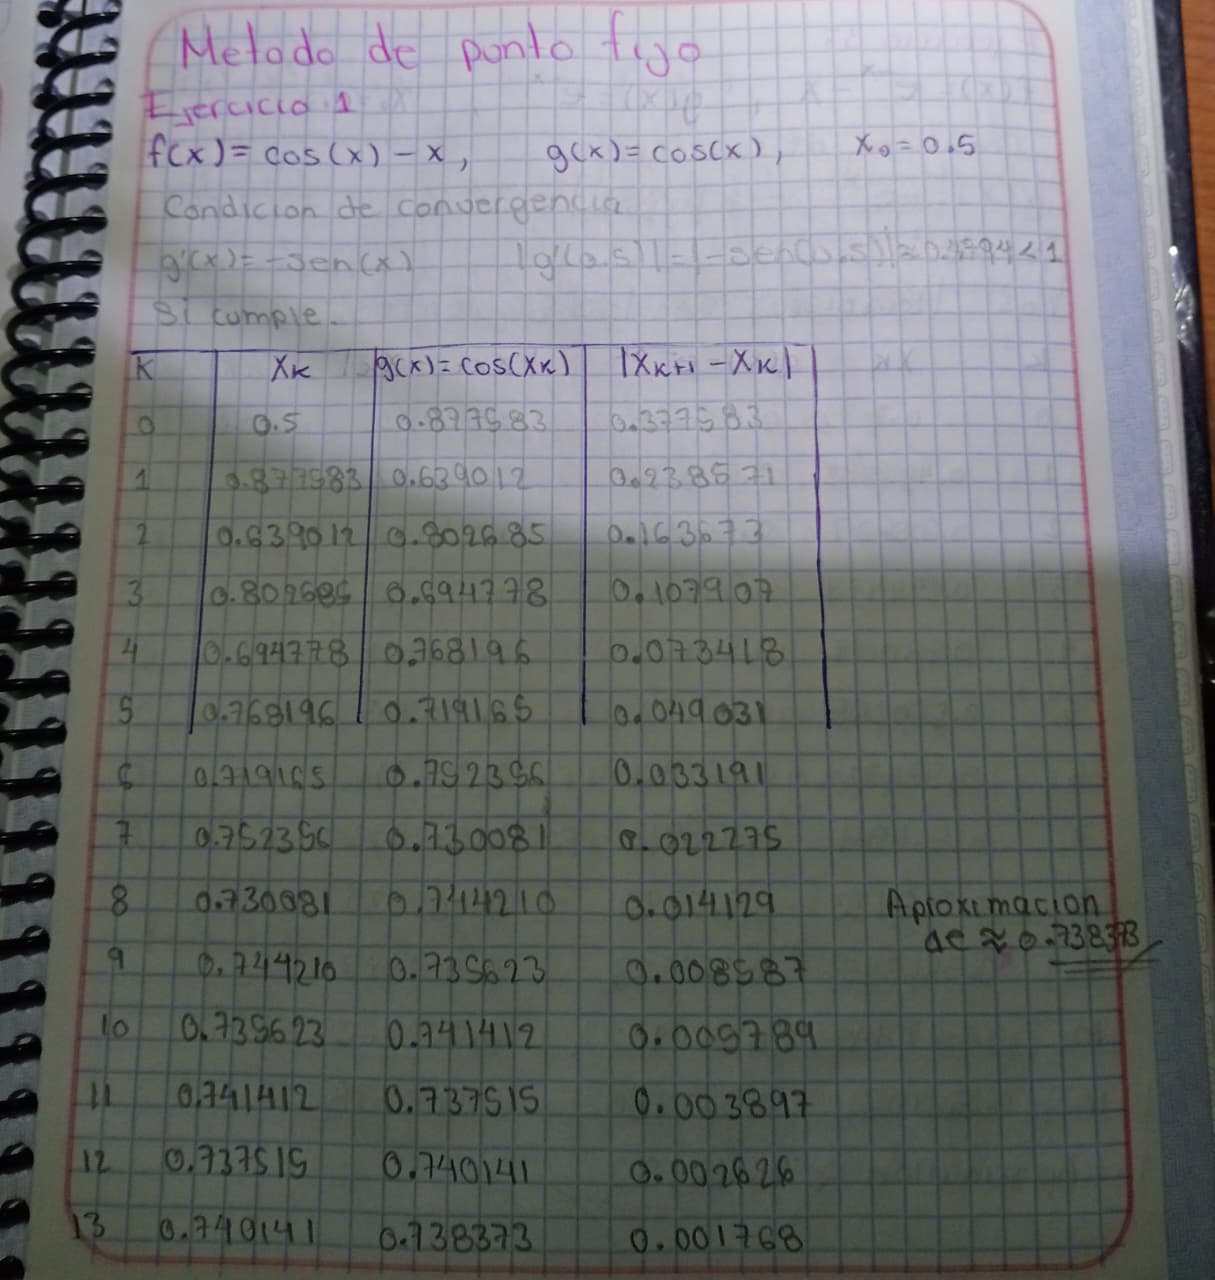
\includegraphics[width=2.60417in,height=\textheight,keepaspectratio,alt={pag.1}]{FIJO_1.jpg}
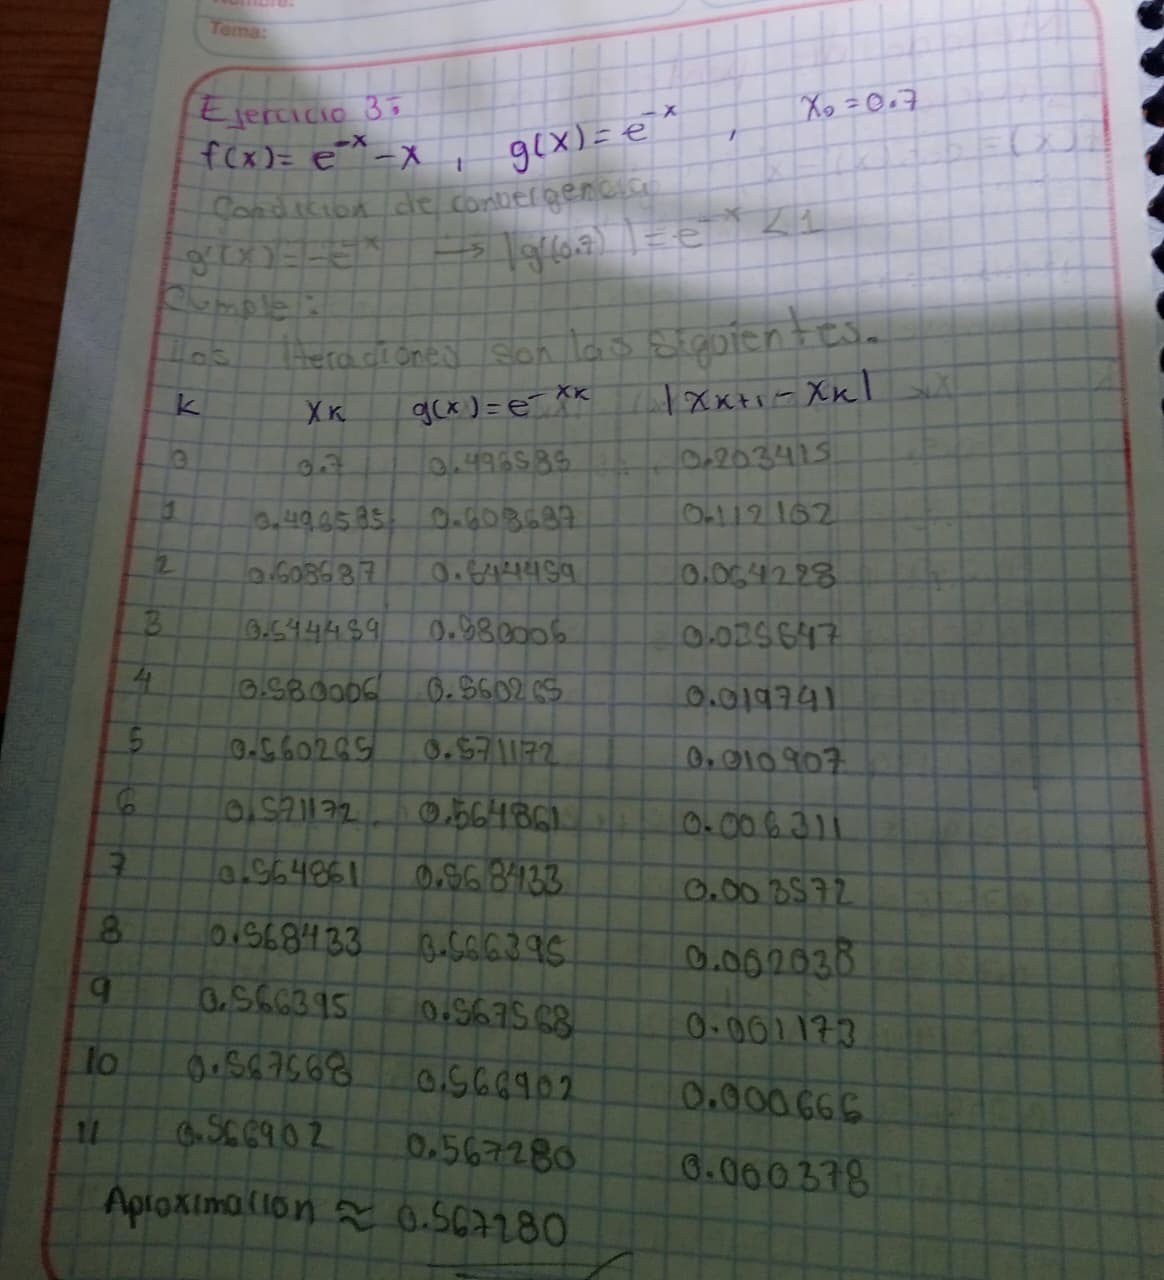
\includegraphics[width=2.60417in,height=\textheight,keepaspectratio,alt={pag.1}]{FIJO_2.jpg}
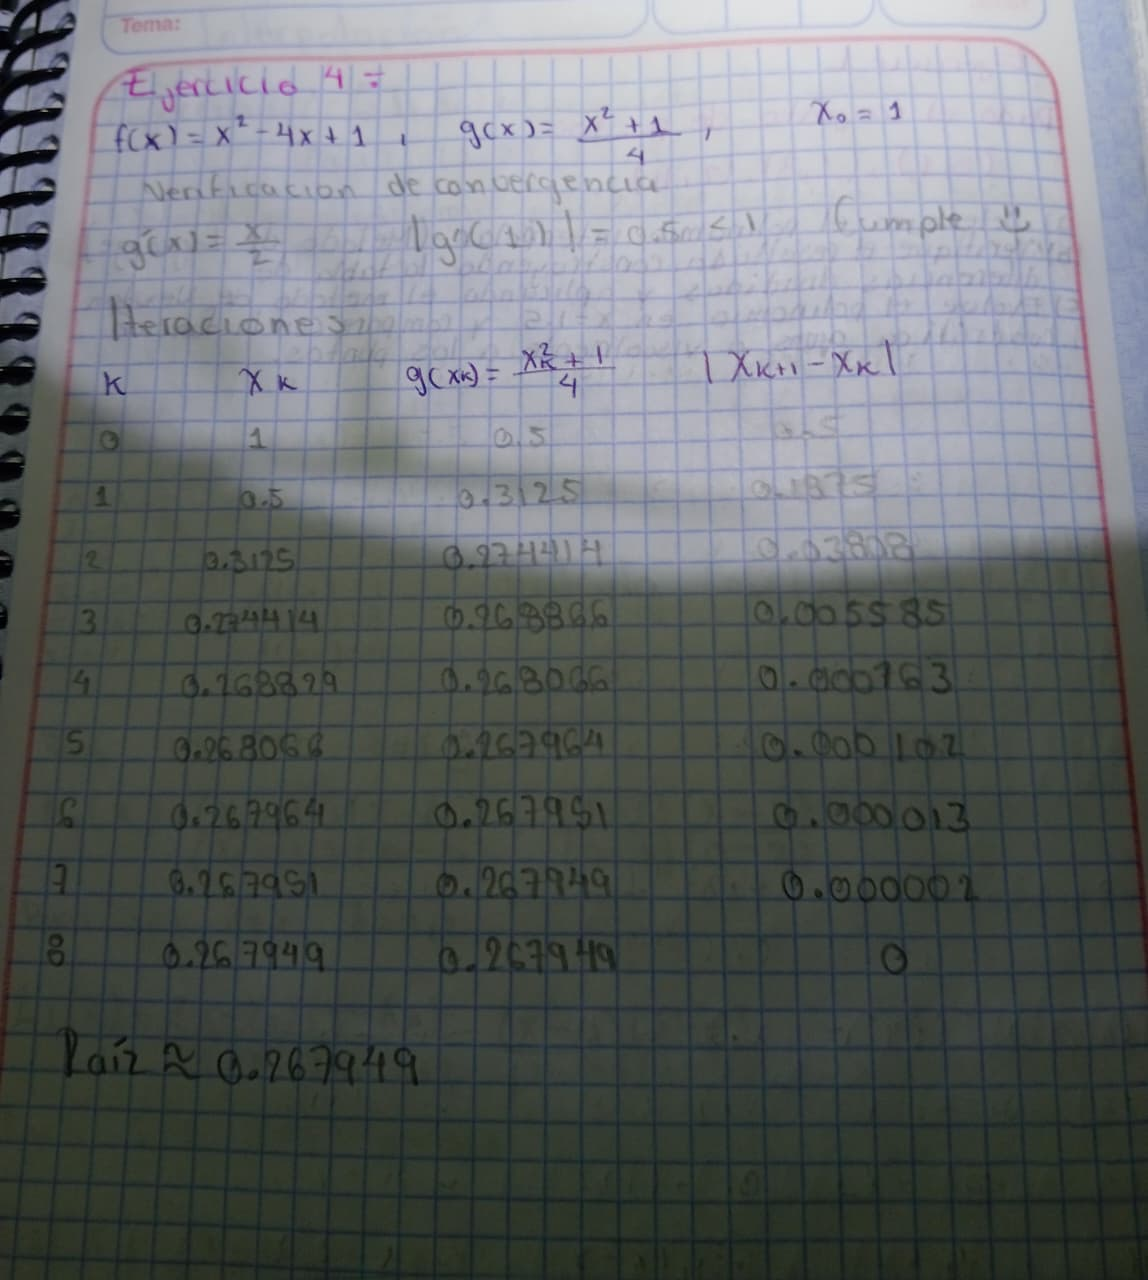
\includegraphics[width=2.60417in,height=\textheight,keepaspectratio,alt={pag.1}]{FIJO_3.jpg}

\subsection{\texorpdfstring{\emph{Ejercicios con
codigo}}{Ejercicios con codigo}}\label{ejercicios-con-codigo}

\begin{Shaded}
\begin{Highlighting}[]
\CommentTok{\# Punto Fijo }

\NormalTok{punto\_fijo\_completo }\OtherTok{\textless{}{-}} \ControlFlowTok{function}\NormalTok{(g, x0, }\AttributeTok{tol =} \FloatTok{1e{-}6}\NormalTok{, }\AttributeTok{iter\_max =} \DecValTok{10}\NormalTok{, }
                               \AttributeTok{nombre\_funcion =} \StringTok{"g(x)"}\NormalTok{, }\AttributeTok{nombre\_latex =} \StringTok{"g(x)"}\NormalTok{) \{}
  
\NormalTok{  iter }\OtherTok{\textless{}{-}} \DecValTok{0}
\NormalTok{  error }\OtherTok{\textless{}{-}} \DecValTok{1}
\NormalTok{  x\_actual }\OtherTok{\textless{}{-}}\NormalTok{ x0}
  
  \CommentTok{\# Crear dataframe para almacenar resultados}
\NormalTok{  resultado }\OtherTok{\textless{}{-}} \FunctionTok{data.frame}\NormalTok{(}
    \AttributeTok{k =} \DecValTok{1}\SpecialCharTok{:}\NormalTok{iter\_max,}
    \AttributeTok{x\_k =} \FunctionTok{numeric}\NormalTok{(iter\_max),}
    \AttributeTok{g\_xk =} \FunctionTok{numeric}\NormalTok{(iter\_max),}
    \AttributeTok{error =} \FunctionTok{numeric}\NormalTok{(iter\_max),}
    \AttributeTok{stringsAsFactors =} \ConstantTok{FALSE}
\NormalTok{  )}
  
\NormalTok{  puntos\_x }\OtherTok{\textless{}{-}} \FunctionTok{numeric}\NormalTok{(iter\_max }\SpecialCharTok{+} \DecValTok{1}\NormalTok{)}
\NormalTok{  puntos\_x[}\DecValTok{1}\NormalTok{] }\OtherTok{\textless{}{-}}\NormalTok{ x0}
\NormalTok{  puntos\_y }\OtherTok{\textless{}{-}} \FunctionTok{numeric}\NormalTok{(iter\_max }\SpecialCharTok{+} \DecValTok{1}\NormalTok{)}
\NormalTok{  puntos\_y[}\DecValTok{1}\NormalTok{] }\OtherTok{\textless{}{-}} \ConstantTok{NA}
  
  \CommentTok{\# Iteraciones del método del punto fijo}
  \ControlFlowTok{for}\NormalTok{ (k }\ControlFlowTok{in} \DecValTok{1}\SpecialCharTok{:}\NormalTok{iter\_max) \{}
\NormalTok{    x\_siguiente }\OtherTok{\textless{}{-}} \FunctionTok{g}\NormalTok{(x\_actual)}
\NormalTok{    error }\OtherTok{\textless{}{-}} \FunctionTok{abs}\NormalTok{(x\_siguiente }\SpecialCharTok{{-}}\NormalTok{ x\_actual)}
    
\NormalTok{    resultado[k, }\DecValTok{2}\SpecialCharTok{:}\DecValTok{4}\NormalTok{] }\OtherTok{\textless{}{-}} \FunctionTok{list}\NormalTok{(x\_actual, x\_siguiente, error)}
\NormalTok{    puntos\_x[k }\SpecialCharTok{+} \DecValTok{1}\NormalTok{] }\OtherTok{\textless{}{-}}\NormalTok{ x\_siguiente}
\NormalTok{    puntos\_y[k }\SpecialCharTok{+} \DecValTok{1}\NormalTok{] }\OtherTok{\textless{}{-}}\NormalTok{ x\_siguiente}
\NormalTok{    x\_actual }\OtherTok{\textless{}{-}}\NormalTok{ x\_siguiente}
    
    \ControlFlowTok{if}\NormalTok{ (error }\SpecialCharTok{\textless{}}\NormalTok{ tol) \{}
\NormalTok{      resultado }\OtherTok{\textless{}{-}}\NormalTok{ resultado[}\DecValTok{1}\SpecialCharTok{:}\NormalTok{k, ]}
\NormalTok{      puntos\_x }\OtherTok{\textless{}{-}}\NormalTok{ puntos\_x[}\DecValTok{1}\SpecialCharTok{:}\NormalTok{(k }\SpecialCharTok{+} \DecValTok{1}\NormalTok{)]}
\NormalTok{      puntos\_y }\OtherTok{\textless{}{-}}\NormalTok{ puntos\_y[}\DecValTok{1}\SpecialCharTok{:}\NormalTok{(k }\SpecialCharTok{+} \DecValTok{1}\NormalTok{)]}
      \ControlFlowTok{break}
\NormalTok{    \}}
\NormalTok{  \}}
  
  \CommentTok{\# Verificar convergencia}
  \ControlFlowTok{if}\NormalTok{ (iter\_max }\SpecialCharTok{\textgreater{}} \DecValTok{1}\NormalTok{) \{}
\NormalTok{    g\_prime }\OtherTok{\textless{}{-}} \FunctionTok{tryCatch}\NormalTok{(\{}
      \CommentTok{\# Aproximación numérica de la derivada}
\NormalTok{      h }\OtherTok{\textless{}{-}} \FloatTok{1e{-}6}
\NormalTok{      (}\FunctionTok{g}\NormalTok{(x0 }\SpecialCharTok{+}\NormalTok{ h) }\SpecialCharTok{{-}} \FunctionTok{g}\NormalTok{(x0)) }\SpecialCharTok{/}\NormalTok{ h}
\NormalTok{    \}, }\AttributeTok{error =} \ControlFlowTok{function}\NormalTok{(e) }\ConstantTok{NA}\NormalTok{)}
    
\NormalTok{    condicion }\OtherTok{\textless{}{-}} \FunctionTok{ifelse}\NormalTok{(}\SpecialCharTok{!}\FunctionTok{is.na}\NormalTok{(g\_prime), }\FunctionTok{abs}\NormalTok{(g\_prime) }\SpecialCharTok{\textless{}} \DecValTok{1}\NormalTok{, }\StringTok{"No se pudo calcular"}\NormalTok{)}
\NormalTok{  \} }\ControlFlowTok{else}\NormalTok{ \{}
\NormalTok{    condicion }\OtherTok{\textless{}{-}} \StringTok{"No evaluado"}
\NormalTok{  \}}
  
  \FunctionTok{return}\NormalTok{(}\FunctionTok{list}\NormalTok{(}
    \AttributeTok{raiz =}\NormalTok{ x\_actual,}
    \AttributeTok{tabla =}\NormalTok{ resultado,}
    \AttributeTok{puntos\_x =}\NormalTok{ puntos\_x,}
    \AttributeTok{puntos\_y =}\NormalTok{ puntos\_y,}
    \AttributeTok{condicion\_convergencia =}\NormalTok{ condicion,}
    \AttributeTok{derivada\_aproximada =} \FunctionTok{ifelse}\NormalTok{(}\FunctionTok{exists}\NormalTok{(}\StringTok{"g\_prime"}\NormalTok{), g\_prime, }\ConstantTok{NA}\NormalTok{)}
\NormalTok{  ))}
\NormalTok{\}}
\end{Highlighting}
\end{Shaded}

\begin{Shaded}
\begin{Highlighting}[]
\CommentTok{\# FUNCIÓN PARA CREAR GRÁFICAS }
\NormalTok{crear\_grafica\_punto\_fijo }\OtherTok{\textless{}{-}} \ControlFlowTok{function}\NormalTok{(g, puntos\_x, nombre\_latex, x\_min, x\_max) \{}
  
  \CommentTok{\# Generar valores para las curvas}
\NormalTok{  x\_vals }\OtherTok{\textless{}{-}} \FunctionTok{seq}\NormalTok{(x\_min, x\_max, }\AttributeTok{length.out =} \DecValTok{400}\NormalTok{)}
\NormalTok{  g\_vals }\OtherTok{\textless{}{-}} \FunctionTok{sapply}\NormalTok{(x\_vals, g)}
  
  \CommentTok{\# Crear gráfica base}
  \FunctionTok{plot}\NormalTok{(x\_vals, g\_vals, }\AttributeTok{type =} \StringTok{"l"}\NormalTok{, }\AttributeTok{lwd =} \DecValTok{3}\NormalTok{, }\AttributeTok{col =} \StringTok{"blue"}\NormalTok{,}
       \AttributeTok{main =} \FunctionTok{paste}\NormalTok{(}\StringTok{"Método del Punto Fijo para"}\NormalTok{, nombre\_latex),}
       \AttributeTok{xlab =} \StringTok{"x"}\NormalTok{, }\AttributeTok{ylab =} \StringTok{"y"}\NormalTok{,}
       \AttributeTok{ylim =} \FunctionTok{range}\NormalTok{(}\FunctionTok{c}\NormalTok{(x\_vals, g\_vals)),}
       \AttributeTok{xlim =} \FunctionTok{c}\NormalTok{(x\_min, x\_max))}
  
  \CommentTok{\# Línea y = x (diagonal)}
  \FunctionTok{lines}\NormalTok{(x\_vals, x\_vals, }\AttributeTok{col =} \StringTok{"red"}\NormalTok{, }\AttributeTok{lwd =} \DecValTok{2}\NormalTok{, }\AttributeTok{lty =} \DecValTok{2}\NormalTok{)}
  
  \CommentTok{\# Ejes}
  \FunctionTok{abline}\NormalTok{(}\AttributeTok{h =} \DecValTok{0}\NormalTok{, }\AttributeTok{v =} \DecValTok{0}\NormalTok{, }\AttributeTok{col =} \StringTok{"gray"}\NormalTok{, }\AttributeTok{lty =} \DecValTok{3}\NormalTok{)}
  
  \CommentTok{\# Puntos de iteración}
\NormalTok{  n\_puntos }\OtherTok{\textless{}{-}} \FunctionTok{length}\NormalTok{(puntos\_x)}
\NormalTok{  colores }\OtherTok{\textless{}{-}} \FunctionTok{rainbow}\NormalTok{(n\_puntos)}
  
  \ControlFlowTok{for}\NormalTok{ (i }\ControlFlowTok{in} \DecValTok{1}\SpecialCharTok{:}\NormalTok{n\_puntos) \{}
\NormalTok{    x\_point }\OtherTok{\textless{}{-}}\NormalTok{ puntos\_x[i]}
\NormalTok{    y\_point }\OtherTok{\textless{}{-}} \FunctionTok{ifelse}\NormalTok{(i }\SpecialCharTok{==} \DecValTok{1}\NormalTok{, }\ConstantTok{NA}\NormalTok{, }\FunctionTok{g}\NormalTok{(puntos\_x[i}\DecValTok{{-}1}\NormalTok{]))}
    
    \ControlFlowTok{if}\NormalTok{ (}\SpecialCharTok{!}\FunctionTok{is.na}\NormalTok{(y\_point)) \{}
      \CommentTok{\# Punto en y = g(x)}
      \FunctionTok{points}\NormalTok{(x\_point, y\_point, }\AttributeTok{col =}\NormalTok{ colores[i], }\AttributeTok{pch =} \DecValTok{19}\NormalTok{, }\AttributeTok{cex =} \FloatTok{1.2}\NormalTok{)}
      
      \CommentTok{\# Línea vertical a y = x}
      \FunctionTok{segments}\NormalTok{(x\_point, y\_point, y\_point, y\_point, }
               \AttributeTok{col =}\NormalTok{ colores[i], }\AttributeTok{lty =} \DecValTok{3}\NormalTok{, }\AttributeTok{lwd =} \DecValTok{1}\NormalTok{)}
      
      \CommentTok{\# Punto en y = x}
      \FunctionTok{points}\NormalTok{(y\_point, y\_point, }\AttributeTok{col =}\NormalTok{ colores[i], }\AttributeTok{pch =} \DecValTok{4}\NormalTok{, }\AttributeTok{cex =} \FloatTok{1.5}\NormalTok{, }\AttributeTok{lwd =} \DecValTok{2}\NormalTok{)}
      
      \CommentTok{\# Línea horizontal a siguiente punto}
      \FunctionTok{segments}\NormalTok{(y\_point, y\_point, y\_point, }\FunctionTok{g}\NormalTok{(y\_point), }
               \AttributeTok{col =}\NormalTok{ colores[i], }\AttributeTok{lty =} \DecValTok{3}\NormalTok{, }\AttributeTok{lwd =} \DecValTok{1}\NormalTok{)}
      
      \CommentTok{\# Etiqueta numérica cada 2 puntos o en el último}
      \ControlFlowTok{if}\NormalTok{ (i }\SpecialCharTok{\%\%} \DecValTok{2} \SpecialCharTok{==} \DecValTok{0} \SpecialCharTok{||}\NormalTok{ i }\SpecialCharTok{==}\NormalTok{ n\_puntos) \{}
        \FunctionTok{text}\NormalTok{(x\_point, y\_point }\SpecialCharTok{+} \FloatTok{0.05}\SpecialCharTok{*}\NormalTok{(x\_max}\SpecialCharTok{{-}}\NormalTok{x\_min), }
             \AttributeTok{labels =}\NormalTok{ i}\DecValTok{{-}1}\NormalTok{, }\AttributeTok{col =}\NormalTok{ colores[i], }\AttributeTok{font =} \DecValTok{2}\NormalTok{, }\AttributeTok{cex =} \FloatTok{0.8}\NormalTok{)}
\NormalTok{      \}}
\NormalTok{    \}}
\NormalTok{  \}}
  
  \CommentTok{\# Raíz final (punto fijo)}
\NormalTok{  raiz\_final }\OtherTok{\textless{}{-}}\NormalTok{ puntos\_x[n\_puntos]}
  \FunctionTok{points}\NormalTok{(raiz\_final, raiz\_final, }\AttributeTok{col =} \StringTok{"darkgreen"}\NormalTok{, }\AttributeTok{pch =} \DecValTok{17}\NormalTok{, }\AttributeTok{cex =} \DecValTok{2}\NormalTok{, }\AttributeTok{lwd =} \DecValTok{3}\NormalTok{)}
  
  \CommentTok{\# Leyenda}
  \FunctionTok{legend}\NormalTok{(}\StringTok{"topright"}\NormalTok{, }
         \AttributeTok{legend =} \FunctionTok{c}\NormalTok{(}\StringTok{"y = g(x)"}\NormalTok{, }\StringTok{"y = x"}\NormalTok{, }\StringTok{"Puntos iteración"}\NormalTok{, }
                    \StringTok{"Trayectoria"}\NormalTok{, }\StringTok{"Raíz (punto fijo)"}\NormalTok{),}
         \AttributeTok{col =} \FunctionTok{c}\NormalTok{(}\StringTok{"blue"}\NormalTok{, }\StringTok{"red"}\NormalTok{, }\StringTok{"purple"}\NormalTok{, }\StringTok{"orange"}\NormalTok{, }\StringTok{"darkgreen"}\NormalTok{),}
         \AttributeTok{lty =} \FunctionTok{c}\NormalTok{(}\DecValTok{1}\NormalTok{, }\DecValTok{2}\NormalTok{, }\ConstantTok{NA}\NormalTok{, }\DecValTok{3}\NormalTok{, }\ConstantTok{NA}\NormalTok{), }
         \AttributeTok{pch =} \FunctionTok{c}\NormalTok{(}\ConstantTok{NA}\NormalTok{, }\ConstantTok{NA}\NormalTok{, }\DecValTok{19}\NormalTok{, }\ConstantTok{NA}\NormalTok{, }\DecValTok{17}\NormalTok{),}
         \AttributeTok{lwd =} \FunctionTok{c}\NormalTok{(}\DecValTok{3}\NormalTok{, }\DecValTok{2}\NormalTok{, }\ConstantTok{NA}\NormalTok{, }\DecValTok{1}\NormalTok{, }\DecValTok{3}\NormalTok{))}
  
  \CommentTok{\# Texto informativo}
  \FunctionTok{text}\NormalTok{(x\_min }\SpecialCharTok{+} \FloatTok{0.1}\SpecialCharTok{*}\NormalTok{(x\_max}\SpecialCharTok{{-}}\NormalTok{x\_min), x\_max }\SpecialCharTok{{-}} \FloatTok{0.1}\SpecialCharTok{*}\NormalTok{(x\_max}\SpecialCharTok{{-}}\NormalTok{x\_min),}
       \FunctionTok{paste}\NormalTok{(}\StringTok{"Raíz ≈"}\NormalTok{, }\FunctionTok{round}\NormalTok{(raiz\_final, }\DecValTok{6}\NormalTok{)), }
       \AttributeTok{col =} \StringTok{"darkgreen"}\NormalTok{, }\AttributeTok{font =} \DecValTok{2}\NormalTok{, }\AttributeTok{adj =} \DecValTok{0}\NormalTok{)}
\NormalTok{\}}
\end{Highlighting}
\end{Shaded}

\subsubsection{Ejercicio 3:}\label{ejercicio-3}

\(f(x) = e^{-x} - x\)

\(g(x) = e^{-x}\)

\(x0 = 0.7\)

\begin{Shaded}
\begin{Highlighting}[]
\NormalTok{g43 }\OtherTok{\textless{}{-}} \ControlFlowTok{function}\NormalTok{(x) }\FunctionTok{exp}\NormalTok{(}\SpecialCharTok{{-}}\NormalTok{x)}
\NormalTok{resultado\_pf43 }\OtherTok{\textless{}{-}} \FunctionTok{punto\_fijo\_completo}\NormalTok{(g43, }\AttributeTok{x0 =} \FloatTok{0.7}\NormalTok{, }\AttributeTok{iter\_max =} \DecValTok{8}\NormalTok{,}
                                      \AttributeTok{nombre\_latex =} \StringTok{"$g(x) = e\^{}\{{-}x\}$"}\NormalTok{)}

\NormalTok{knitr}\SpecialCharTok{::}\FunctionTok{kable}\NormalTok{(resultado\_pf43}\SpecialCharTok{$}\NormalTok{tabla, }\AttributeTok{digits =} \DecValTok{6}\NormalTok{,}
             \AttributeTok{caption =} \StringTok{"Iteraciones del método del Punto Fijo para $g(x) = e\^{}\{{-}x\}$"}\NormalTok{)}
\end{Highlighting}
\end{Shaded}

\begin{longtable}[]{@{}rrrr@{}}
\caption{Iteraciones del método del Punto Fijo para
\(g(x) = e^{-x}\)}\tabularnewline
\toprule\noalign{}
k & x\_k & g\_xk & error \\
\midrule\noalign{}
\endfirsthead
\toprule\noalign{}
k & x\_k & g\_xk & error \\
\midrule\noalign{}
\endhead
\bottomrule\noalign{}
\endlastfoot
1 & 0.700000 & 0.496585 & 0.203415 \\
2 & 0.496585 & 0.608605 & 0.112020 \\
3 & 0.608605 & 0.544109 & 0.064496 \\
4 & 0.544109 & 0.580359 & 0.036249 \\
5 & 0.580359 & 0.559698 & 0.020661 \\
6 & 0.559698 & 0.571382 & 0.011684 \\
7 & 0.571382 & 0.564745 & 0.006637 \\
8 & 0.564745 & 0.568505 & 0.003761 \\
\end{longtable}

\begin{Shaded}
\begin{Highlighting}[]
\FunctionTok{cat}\NormalTok{(}\StringTok{"Raíz aproximada:"}\NormalTok{, }\FunctionTok{round}\NormalTok{(resultado\_pf43}\SpecialCharTok{$}\NormalTok{raiz, }\DecValTok{8}\NormalTok{), }\StringTok{"}\SpecialCharTok{\textbackslash{}n}\StringTok{"}\NormalTok{)}
\end{Highlighting}
\end{Shaded}

\begin{verbatim}
## Raíz aproximada: 0.5685054
\end{verbatim}

\begin{Shaded}
\begin{Highlighting}[]
\FunctionTok{cat}\NormalTok{(}\StringTok{"Iteraciones realizadas:"}\NormalTok{, }\FunctionTok{nrow}\NormalTok{(resultado\_pf43}\SpecialCharTok{$}\NormalTok{tabla), }\StringTok{"}\SpecialCharTok{\textbackslash{}n}\StringTok{"}\NormalTok{)}
\end{Highlighting}
\end{Shaded}

\begin{verbatim}
## Iteraciones realizadas: 8
\end{verbatim}

\begin{Shaded}
\begin{Highlighting}[]
\FunctionTok{cat}\NormalTok{(}\StringTok{"Error final:"}\NormalTok{, resultado\_pf43}\SpecialCharTok{$}\NormalTok{tabla}\SpecialCharTok{$}\NormalTok{error[}\FunctionTok{nrow}\NormalTok{(resultado\_pf43}\SpecialCharTok{$}\NormalTok{tabla)], }\StringTok{"}\SpecialCharTok{\textbackslash{}n}\StringTok{"}\NormalTok{)}
\end{Highlighting}
\end{Shaded}

\begin{verbatim}
## Error final: 0.003760817
\end{verbatim}

\begin{Shaded}
\begin{Highlighting}[]
\FunctionTok{cat}\NormalTok{(}\StringTok{"Condición |g\textquotesingle{}(x0)| \textless{} 1?:"}\NormalTok{, resultado\_pf43}\SpecialCharTok{$}\NormalTok{condicion\_convergencia, }\StringTok{"}\SpecialCharTok{\textbackslash{}n}\StringTok{"}\NormalTok{)}
\end{Highlighting}
\end{Shaded}

\begin{verbatim}
## Condición |g'(x0)| < 1?: TRUE
\end{verbatim}

\begin{Shaded}
\begin{Highlighting}[]
\FunctionTok{crear\_grafica\_punto\_fijo}\NormalTok{(g43, resultado\_pf43}\SpecialCharTok{$}\NormalTok{puntos\_x,}
                        \StringTok{"$g(x) = e\^{}\{{-}x\}$"}\NormalTok{, }\AttributeTok{x\_min =} \FloatTok{0.4}\NormalTok{, }\AttributeTok{x\_max =} \DecValTok{1}\NormalTok{)}
\end{Highlighting}
\end{Shaded}

\pandocbounded{\includegraphics[keepaspectratio]{Notas_MN_LILIANA_CS_files/figure-latex/unnamed-chunk-491-1.pdf}}

\subsubsection{Ejercicio 2:}\label{ejercicio-2-1}

\(f(x) = x^3 + x - 1\)

\(g(x) = 1 - x^3\)

\(x0 = 0.6\)

\begin{Shaded}
\begin{Highlighting}[]
\NormalTok{g42 }\OtherTok{\textless{}{-}} \ControlFlowTok{function}\NormalTok{(x) }\DecValTok{1} \SpecialCharTok{{-}}\NormalTok{ x}\SpecialCharTok{\^{}}\DecValTok{3}
\NormalTok{resultado\_pf42 }\OtherTok{\textless{}{-}} \FunctionTok{punto\_fijo\_completo}\NormalTok{(g42, }\AttributeTok{x0 =} \FloatTok{0.6}\NormalTok{, }\AttributeTok{iter\_max =} \DecValTok{10}\NormalTok{,}
                                      \AttributeTok{nombre\_latex =} \StringTok{"$g(x) = 1 {-} x\^{}3$"}\NormalTok{)}

\NormalTok{knitr}\SpecialCharTok{::}\FunctionTok{kable}\NormalTok{(resultado\_pf42}\SpecialCharTok{$}\NormalTok{tabla, }\AttributeTok{digits =} \DecValTok{6}\NormalTok{,}
             \AttributeTok{caption =} \StringTok{"Iteraciones del método del Punto Fijo para $g(x) = 1 {-} x\^{}3$"}\NormalTok{)}
\end{Highlighting}
\end{Shaded}

\begin{longtable}[]{@{}rrrr@{}}
\caption{Iteraciones del método del Punto Fijo para
\(g(x) = 1 - x^3\)}\tabularnewline
\toprule\noalign{}
k & x\_k & g\_xk & error \\
\midrule\noalign{}
\endfirsthead
\toprule\noalign{}
k & x\_k & g\_xk & error \\
\midrule\noalign{}
\endhead
\bottomrule\noalign{}
\endlastfoot
1 & 0.600000 & 0.784000 & 0.184000 \\
2 & 0.784000 & 0.518110 & 0.265890 \\
3 & 0.518110 & 0.860920 & 0.342810 \\
4 & 0.860920 & 0.361901 & 0.499019 \\
5 & 0.361901 & 0.952601 & 0.590700 \\
6 & 0.952601 & 0.135563 & 0.817038 \\
7 & 0.135563 & 0.997509 & 0.861945 \\
8 & 0.997509 & 0.007455 & 0.990053 \\
9 & 0.007455 & 1.000000 & 0.992544 \\
10 & 1.000000 & 0.000001 & 0.999998 \\
\end{longtable}

\begin{Shaded}
\begin{Highlighting}[]
\FunctionTok{cat}\NormalTok{(}\StringTok{"Raíz aproximada:"}\NormalTok{, }\FunctionTok{round}\NormalTok{(resultado\_pf42}\SpecialCharTok{$}\NormalTok{raiz, }\DecValTok{8}\NormalTok{), }\StringTok{"}\SpecialCharTok{\textbackslash{}n}\StringTok{"}\NormalTok{)}
\end{Highlighting}
\end{Shaded}

\begin{verbatim}
## Raíz aproximada: 1.24e-06
\end{verbatim}

\begin{Shaded}
\begin{Highlighting}[]
\FunctionTok{cat}\NormalTok{(}\StringTok{"Iteraciones realizadas:"}\NormalTok{, }\FunctionTok{nrow}\NormalTok{(resultado\_pf42}\SpecialCharTok{$}\NormalTok{tabla), }\StringTok{"}\SpecialCharTok{\textbackslash{}n}\StringTok{"}\NormalTok{)}
\end{Highlighting}
\end{Shaded}

\begin{verbatim}
## Iteraciones realizadas: 10
\end{verbatim}

\begin{Shaded}
\begin{Highlighting}[]
\FunctionTok{cat}\NormalTok{(}\StringTok{"Error final:"}\NormalTok{, resultado\_pf42}\SpecialCharTok{$}\NormalTok{tabla}\SpecialCharTok{$}\NormalTok{error[}\FunctionTok{nrow}\NormalTok{(resultado\_pf42}\SpecialCharTok{$}\NormalTok{tabla)], }\StringTok{"}\SpecialCharTok{\textbackslash{}n}\StringTok{"}\NormalTok{)}
\end{Highlighting}
\end{Shaded}

\begin{verbatim}
## Error final: 0.9999983
\end{verbatim}

\begin{Shaded}
\begin{Highlighting}[]
\FunctionTok{cat}\NormalTok{(}\StringTok{"Condición |g\textquotesingle{}(x0)| \textless{} 1?:"}\NormalTok{, resultado\_pf42}\SpecialCharTok{$}\NormalTok{condicion\_convergencia, }\StringTok{"}\SpecialCharTok{\textbackslash{}n}\StringTok{"}\NormalTok{)}
\end{Highlighting}
\end{Shaded}

\begin{verbatim}
## Condición |g'(x0)| < 1?: FALSE
\end{verbatim}

\begin{Shaded}
\begin{Highlighting}[]
\FunctionTok{crear\_grafica\_punto\_fijo}\NormalTok{(g42, resultado\_pf42}\SpecialCharTok{$}\NormalTok{puntos\_x,}
                        \StringTok{"$g(x) = 1 {-} x\^{}3$"}\NormalTok{, }\AttributeTok{x\_min =} \DecValTok{0}\NormalTok{, }\AttributeTok{x\_max =} \FloatTok{1.5}\NormalTok{)}
\end{Highlighting}
\end{Shaded}

\pandocbounded{\includegraphics[keepaspectratio]{Notas_MN_LILIANA_CS_files/figure-latex/unnamed-chunk-493-1.pdf}}

\subsubsection{Ejercicio 4:}\label{ejercicio-4-1}

\(f(x) = x^2 - 4x + 1\)

\(g(x) = (x^2 + 1)/4\)

\(x0 = 1\)

\begin{Shaded}
\begin{Highlighting}[]
\NormalTok{g44 }\OtherTok{\textless{}{-}} \ControlFlowTok{function}\NormalTok{(x) (x}\SpecialCharTok{\^{}}\DecValTok{2} \SpecialCharTok{+} \DecValTok{1}\NormalTok{)}\SpecialCharTok{/}\DecValTok{4}
\NormalTok{resultado\_pf44 }\OtherTok{\textless{}{-}} \FunctionTok{punto\_fijo\_completo}\NormalTok{(g44, }\AttributeTok{x0 =} \DecValTok{1}\NormalTok{, }\AttributeTok{iter\_max =} \DecValTok{8}\NormalTok{,}
                                      \AttributeTok{nombre\_latex =} \StringTok{"$g(x) = }\SpecialCharTok{\textbackslash{}\textbackslash{}}\StringTok{frac\{x\^{}2 + 1\}\{4\}$"}\NormalTok{)}

\NormalTok{knitr}\SpecialCharTok{::}\FunctionTok{kable}\NormalTok{(resultado\_pf44}\SpecialCharTok{$}\NormalTok{tabla, }\AttributeTok{digits =} \DecValTok{6}\NormalTok{,}
             \AttributeTok{caption =} \StringTok{"Iteraciones del método del Punto Fijo para $g(x) = }\SpecialCharTok{\textbackslash{}\textbackslash{}}\StringTok{frac\{x\^{}2 + 1\}\{4\}$"}\NormalTok{)}
\end{Highlighting}
\end{Shaded}

\begin{longtable}[]{@{}rrrr@{}}
\caption{Iteraciones del método del Punto Fijo para
\(g(x) = \frac{x^2 + 1}{4}\)}\tabularnewline
\toprule\noalign{}
k & x\_k & g\_xk & error \\
\midrule\noalign{}
\endfirsthead
\toprule\noalign{}
k & x\_k & g\_xk & error \\
\midrule\noalign{}
\endhead
\bottomrule\noalign{}
\endlastfoot
1 & 1.000000 & 0.500000 & 0.500000 \\
2 & 0.500000 & 0.312500 & 0.187500 \\
3 & 0.312500 & 0.274414 & 0.038086 \\
4 & 0.274414 & 0.268826 & 0.005588 \\
5 & 0.268826 & 0.268067 & 0.000759 \\
6 & 0.268067 & 0.267965 & 0.000102 \\
7 & 0.267965 & 0.267951 & 0.000014 \\
8 & 0.267951 & 0.267949 & 0.000002 \\
\end{longtable}

\begin{Shaded}
\begin{Highlighting}[]
\FunctionTok{cat}\NormalTok{(}\StringTok{"Raíz aproximada:"}\NormalTok{, }\FunctionTok{round}\NormalTok{(resultado\_pf44}\SpecialCharTok{$}\NormalTok{raiz, }\DecValTok{8}\NormalTok{), }\StringTok{"}\SpecialCharTok{\textbackslash{}n}\StringTok{"}\NormalTok{)}
\end{Highlighting}
\end{Shaded}

\begin{verbatim}
## Raíz aproximada: 0.2679495
\end{verbatim}

\begin{Shaded}
\begin{Highlighting}[]
\FunctionTok{cat}\NormalTok{(}\StringTok{"Iteraciones realizadas:"}\NormalTok{, }\FunctionTok{nrow}\NormalTok{(resultado\_pf44}\SpecialCharTok{$}\NormalTok{tabla), }\StringTok{"}\SpecialCharTok{\textbackslash{}n}\StringTok{"}\NormalTok{)}
\end{Highlighting}
\end{Shaded}

\begin{verbatim}
## Iteraciones realizadas: 8
\end{verbatim}

\begin{Shaded}
\begin{Highlighting}[]
\FunctionTok{cat}\NormalTok{(}\StringTok{"Error final:"}\NormalTok{, resultado\_pf44}\SpecialCharTok{$}\NormalTok{tabla}\SpecialCharTok{$}\NormalTok{error[}\FunctionTok{nrow}\NormalTok{(resultado\_pf44}\SpecialCharTok{$}\NormalTok{tabla)], }\StringTok{"}\SpecialCharTok{\textbackslash{}n}\StringTok{"}\NormalTok{)}
\end{Highlighting}
\end{Shaded}

\begin{verbatim}
## Error final: 1.828966e-06
\end{verbatim}

\begin{Shaded}
\begin{Highlighting}[]
\FunctionTok{cat}\NormalTok{(}\StringTok{"Condición |g\textquotesingle{}(x0)| \textless{} 1?:"}\NormalTok{, resultado\_pf44}\SpecialCharTok{$}\NormalTok{condicion\_convergencia, }\StringTok{"}\SpecialCharTok{\textbackslash{}n}\StringTok{"}\NormalTok{)}
\end{Highlighting}
\end{Shaded}

\begin{verbatim}
## Condición |g'(x0)| < 1?: TRUE
\end{verbatim}

\begin{Shaded}
\begin{Highlighting}[]
\FunctionTok{crear\_grafica\_punto\_fijo}\NormalTok{(g44, resultado\_pf44}\SpecialCharTok{$}\NormalTok{puntos\_x,}
                        \StringTok{"$g(x) = }\SpecialCharTok{\textbackslash{}\textbackslash{}}\StringTok{frac\{x\^{}2 + 1\}\{4\}$"}\NormalTok{, }\AttributeTok{x\_min =} \DecValTok{0}\NormalTok{, }\AttributeTok{x\_max =} \FloatTok{1.5}\NormalTok{)}
\end{Highlighting}
\end{Shaded}

\pandocbounded{\includegraphics[keepaspectratio]{Notas_MN_LILIANA_CS_files/figure-latex/unnamed-chunk-495-1.pdf}}

\subsubsection{Ejercicio 9:}\label{ejercicio-9}

\(f(x) = x - sin(x) - 1\)

\(g(x) = sin(x) + 1\)

\(x0 = 1\)

\begin{Shaded}
\begin{Highlighting}[]
\NormalTok{g9 }\OtherTok{\textless{}{-}} \ControlFlowTok{function}\NormalTok{(x) }\FunctionTok{sin}\NormalTok{(x) }\SpecialCharTok{+} \DecValTok{1}
\NormalTok{resultado\_pf9 }\OtherTok{\textless{}{-}} \FunctionTok{punto\_fijo\_completo}\NormalTok{(g9, }\AttributeTok{x0 =} \DecValTok{1}\NormalTok{, }\AttributeTok{iter\_max =} \DecValTok{10}\NormalTok{,}
                                     \AttributeTok{nombre\_latex =} \StringTok{"$g(x) = }\SpecialCharTok{\textbackslash{}\textbackslash{}}\StringTok{sin(x) + 1$"}\NormalTok{)}

\NormalTok{knitr}\SpecialCharTok{::}\FunctionTok{kable}\NormalTok{(resultado\_pf9}\SpecialCharTok{$}\NormalTok{tabla, }\AttributeTok{digits =} \DecValTok{6}\NormalTok{,}
             \AttributeTok{caption =} \StringTok{"Iteraciones del método del Punto Fijo para $g(x) = }\SpecialCharTok{\textbackslash{}\textbackslash{}}\StringTok{sin(x) + 1$"}\NormalTok{)}
\end{Highlighting}
\end{Shaded}

\begin{longtable}[]{@{}rrrr@{}}
\caption{Iteraciones del método del Punto Fijo para
\(g(x) = \sin(x) + 1\)}\tabularnewline
\toprule\noalign{}
k & x\_k & g\_xk & error \\
\midrule\noalign{}
\endfirsthead
\toprule\noalign{}
k & x\_k & g\_xk & error \\
\midrule\noalign{}
\endhead
\bottomrule\noalign{}
\endlastfoot
1 & 1.000000 & 1.841471 & 0.841471 \\
2 & 1.841471 & 1.963591 & 0.122120 \\
3 & 1.963591 & 1.923843 & 0.039748 \\
4 & 1.923843 & 1.938324 & 0.014481 \\
5 & 1.938324 & 1.933219 & 0.005105 \\
6 & 1.933219 & 1.935041 & 0.001822 \\
7 & 1.935041 & 1.934393 & 0.000648 \\
8 & 1.934393 & 1.934624 & 0.000230 \\
9 & 1.934624 & 1.934542 & 0.000082 \\
10 & 1.934542 & 1.934571 & 0.000029 \\
\end{longtable}

\begin{Shaded}
\begin{Highlighting}[]
\FunctionTok{cat}\NormalTok{(}\StringTok{"Raíz aproximada:"}\NormalTok{, }\FunctionTok{round}\NormalTok{(resultado\_pf9}\SpecialCharTok{$}\NormalTok{raiz, }\DecValTok{8}\NormalTok{), }\StringTok{"}\SpecialCharTok{\textbackslash{}n}\StringTok{"}\NormalTok{)}
\end{Highlighting}
\end{Shaded}

\begin{verbatim}
## Raíz aproximada: 1.934571
\end{verbatim}

\begin{Shaded}
\begin{Highlighting}[]
\FunctionTok{cat}\NormalTok{(}\StringTok{"Iteraciones realizadas:"}\NormalTok{, }\FunctionTok{nrow}\NormalTok{(resultado\_pf9}\SpecialCharTok{$}\NormalTok{tabla), }\StringTok{"}\SpecialCharTok{\textbackslash{}n}\StringTok{"}\NormalTok{)}
\end{Highlighting}
\end{Shaded}

\begin{verbatim}
## Iteraciones realizadas: 10
\end{verbatim}

\begin{Shaded}
\begin{Highlighting}[]
\FunctionTok{cat}\NormalTok{(}\StringTok{"Error final:"}\NormalTok{, resultado\_pf9}\SpecialCharTok{$}\NormalTok{tabla}\SpecialCharTok{$}\NormalTok{error[}\FunctionTok{nrow}\NormalTok{(resultado\_pf9}\SpecialCharTok{$}\NormalTok{tabla)], }\StringTok{"}\SpecialCharTok{\textbackslash{}n}\StringTok{"}\NormalTok{)}
\end{Highlighting}
\end{Shaded}

\begin{verbatim}
## Error final: 2.917573e-05
\end{verbatim}

\begin{Shaded}
\begin{Highlighting}[]
\FunctionTok{cat}\NormalTok{(}\StringTok{"Condición |g\textquotesingle{}(x0)| \textless{} 1?:"}\NormalTok{, resultado\_pf9}\SpecialCharTok{$}\NormalTok{condicion\_convergencia, }\StringTok{"}\SpecialCharTok{\textbackslash{}n}\StringTok{"}\NormalTok{)}
\end{Highlighting}
\end{Shaded}

\begin{verbatim}
## Condición |g'(x0)| < 1?: TRUE
\end{verbatim}

\begin{Shaded}
\begin{Highlighting}[]
\FunctionTok{crear\_grafica\_punto\_fijo}\NormalTok{(g9, resultado\_pf9}\SpecialCharTok{$}\NormalTok{puntos\_x,}
                        \StringTok{"$g(x) = }\SpecialCharTok{\textbackslash{}\textbackslash{}}\StringTok{sin(x) + 1$"}\NormalTok{, }\AttributeTok{x\_min =} \FloatTok{0.5}\NormalTok{, }\AttributeTok{x\_max =} \FloatTok{2.5}\NormalTok{)}
\end{Highlighting}
\end{Shaded}

\pandocbounded{\includegraphics[keepaspectratio]{Notas_MN_LILIANA_CS_files/figure-latex/unnamed-chunk-497-1.pdf}}

\subsubsection{Ejercicio 12:}\label{ejercicio-12-1}

\(f(x) = x^3 + 4x^2 - 10\)

\(g(x) = sqrt((10 - x^3)/4)\)

\(x0 = 1.5\)

\begin{Shaded}
\begin{Highlighting}[]
\NormalTok{g12 }\OtherTok{\textless{}{-}} \ControlFlowTok{function}\NormalTok{(x) }\FunctionTok{sqrt}\NormalTok{((}\DecValTok{10} \SpecialCharTok{{-}}\NormalTok{ x}\SpecialCharTok{\^{}}\DecValTok{3}\NormalTok{)}\SpecialCharTok{/}\DecValTok{4}\NormalTok{)}
\NormalTok{resultado\_pf12 }\OtherTok{\textless{}{-}} \FunctionTok{punto\_fijo\_completo}\NormalTok{(g12, }\AttributeTok{x0 =} \FloatTok{1.5}\NormalTok{, }\AttributeTok{iter\_max =} \DecValTok{10}\NormalTok{,}
                                      \AttributeTok{nombre\_latex =} \StringTok{"$g(x) = }\SpecialCharTok{\textbackslash{}\textbackslash{}}\StringTok{sqrt\{}\SpecialCharTok{\textbackslash{}\textbackslash{}}\StringTok{frac\{10 {-} x\^{}3\}\{4\}\}$"}\NormalTok{)}

\NormalTok{knitr}\SpecialCharTok{::}\FunctionTok{kable}\NormalTok{(resultado\_pf12}\SpecialCharTok{$}\NormalTok{tabla, }\AttributeTok{digits =} \DecValTok{6}\NormalTok{,}
             \AttributeTok{caption =} \StringTok{"Iteraciones del método del Punto Fijo para $g(x) = }\SpecialCharTok{\textbackslash{}\textbackslash{}}\StringTok{sqrt\{}\SpecialCharTok{\textbackslash{}\textbackslash{}}\StringTok{frac\{10 {-} x\^{}3\}\{4\}\}$"}\NormalTok{)}
\end{Highlighting}
\end{Shaded}

\begin{longtable}[]{@{}rrrr@{}}
\caption{Iteraciones del método del Punto Fijo para
\(g(x) = \sqrt{\frac{10 - x^3}{4}}\)}\tabularnewline
\toprule\noalign{}
k & x\_k & g\_xk & error \\
\midrule\noalign{}
\endfirsthead
\toprule\noalign{}
k & x\_k & g\_xk & error \\
\midrule\noalign{}
\endhead
\bottomrule\noalign{}
\endlastfoot
1 & 1.500000 & 1.286954 & 0.213046 \\
2 & 1.286954 & 1.402541 & 0.115587 \\
3 & 1.402541 & 1.345458 & 0.057082 \\
4 & 1.345458 & 1.375170 & 0.029712 \\
5 & 1.375170 & 1.360094 & 0.015076 \\
6 & 1.360094 & 1.367847 & 0.007753 \\
7 & 1.367847 & 1.363887 & 0.003960 \\
8 & 1.363887 & 1.365917 & 0.002030 \\
9 & 1.365917 & 1.364878 & 0.001039 \\
10 & 1.364878 & 1.365410 & 0.000532 \\
\end{longtable}

\begin{Shaded}
\begin{Highlighting}[]
\FunctionTok{cat}\NormalTok{(}\StringTok{"Raíz aproximada:"}\NormalTok{, }\FunctionTok{round}\NormalTok{(resultado\_pf12}\SpecialCharTok{$}\NormalTok{raiz, }\DecValTok{8}\NormalTok{), }\StringTok{"}\SpecialCharTok{\textbackslash{}n}\StringTok{"}\NormalTok{)}
\end{Highlighting}
\end{Shaded}

\begin{verbatim}
## Raíz aproximada: 1.36541
\end{verbatim}

\begin{Shaded}
\begin{Highlighting}[]
\FunctionTok{cat}\NormalTok{(}\StringTok{"Iteraciones realizadas:"}\NormalTok{, }\FunctionTok{nrow}\NormalTok{(resultado\_pf12}\SpecialCharTok{$}\NormalTok{tabla), }\StringTok{"}\SpecialCharTok{\textbackslash{}n}\StringTok{"}\NormalTok{)}
\end{Highlighting}
\end{Shaded}

\begin{verbatim}
## Iteraciones realizadas: 10
\end{verbatim}

\begin{Shaded}
\begin{Highlighting}[]
\FunctionTok{cat}\NormalTok{(}\StringTok{"Error final:"}\NormalTok{, resultado\_pf12}\SpecialCharTok{$}\NormalTok{tabla}\SpecialCharTok{$}\NormalTok{error[}\FunctionTok{nrow}\NormalTok{(resultado\_pf12}\SpecialCharTok{$}\NormalTok{tabla)], }\StringTok{"}\SpecialCharTok{\textbackslash{}n}\StringTok{"}\NormalTok{)}
\end{Highlighting}
\end{Shaded}

\begin{verbatim}
## Error final: 0.000531844
\end{verbatim}

\begin{Shaded}
\begin{Highlighting}[]
\FunctionTok{cat}\NormalTok{(}\StringTok{"Condición |g\textquotesingle{}(x0)| \textless{} 1?:"}\NormalTok{, resultado\_pf12}\SpecialCharTok{$}\NormalTok{condicion\_convergencia, }\StringTok{"}\SpecialCharTok{\textbackslash{}n}\StringTok{"}\NormalTok{)}
\end{Highlighting}
\end{Shaded}

\begin{verbatim}
## Condición |g'(x0)| < 1?: TRUE
\end{verbatim}

\begin{Shaded}
\begin{Highlighting}[]
\FunctionTok{cat}\NormalTok{(}\StringTok{"|g\textquotesingle{}(x0)| aproximado:"}\NormalTok{, }\FunctionTok{round}\NormalTok{(}\FunctionTok{abs}\NormalTok{(resultado\_pf12}\SpecialCharTok{$}\NormalTok{derivada\_aproximada), }\DecValTok{6}\NormalTok{), }\StringTok{"}\SpecialCharTok{\textbackslash{}n}\StringTok{"}\NormalTok{)}
\end{Highlighting}
\end{Shaded}

\begin{verbatim}
## |g'(x0)| aproximado: 0.655619
\end{verbatim}

\begin{Shaded}
\begin{Highlighting}[]
\FunctionTok{crear\_grafica\_punto\_fijo}\NormalTok{(g12, resultado\_pf12}\SpecialCharTok{$}\NormalTok{puntos\_x,}
                        \StringTok{"$g(x) = }\SpecialCharTok{\textbackslash{}\textbackslash{}}\StringTok{sqrt\{}\SpecialCharTok{\textbackslash{}\textbackslash{}}\StringTok{frac\{10 {-} x\^{}3\}\{4\}\}$"}\NormalTok{, }\AttributeTok{x\_min =} \DecValTok{1}\NormalTok{, }\AttributeTok{x\_max =} \DecValTok{2}\NormalTok{)}
\end{Highlighting}
\end{Shaded}

\pandocbounded{\includegraphics[keepaspectratio]{Notas_MN_LILIANA_CS_files/figure-latex/unnamed-chunk-499-1.pdf}}

\subsubsection{Ejercicio 14:}\label{ejercicio-14}

\(f(x) = x - e^{-x^2}\)

\(g(x) = e^{-x^2}\)

\(x0 = 0.5\)

\begin{Shaded}
\begin{Highlighting}[]
\NormalTok{g14 }\OtherTok{\textless{}{-}} \ControlFlowTok{function}\NormalTok{(x) }\FunctionTok{exp}\NormalTok{(}\SpecialCharTok{{-}}\NormalTok{x}\SpecialCharTok{\^{}}\DecValTok{2}\NormalTok{)}
\NormalTok{resultado\_pf14 }\OtherTok{\textless{}{-}} \FunctionTok{punto\_fijo\_completo}\NormalTok{(g14, }\AttributeTok{x0 =} \FloatTok{0.5}\NormalTok{, }\AttributeTok{iter\_max =} \DecValTok{10}\NormalTok{,}
                                      \AttributeTok{nombre\_latex =} \StringTok{"$g(x) = e\^{}\{{-}x\^{}2\}$"}\NormalTok{)}

\NormalTok{knitr}\SpecialCharTok{::}\FunctionTok{kable}\NormalTok{(resultado\_pf14}\SpecialCharTok{$}\NormalTok{tabla, }\AttributeTok{digits =} \DecValTok{6}\NormalTok{,}
             \AttributeTok{caption =} \StringTok{"Iteraciones del método del Punto Fijo para $g(x) = e\^{}\{{-}x\^{}2\}$"}\NormalTok{)}
\end{Highlighting}
\end{Shaded}

\begin{longtable}[]{@{}rrrr@{}}
\caption{Iteraciones del método del Punto Fijo para
\(g(x) = e^{-x^2}\)}\tabularnewline
\toprule\noalign{}
k & x\_k & g\_xk & error \\
\midrule\noalign{}
\endfirsthead
\toprule\noalign{}
k & x\_k & g\_xk & error \\
\midrule\noalign{}
\endhead
\bottomrule\noalign{}
\endlastfoot
1 & 0.500000 & 0.778801 & 0.278801 \\
2 & 0.778801 & 0.545239 & 0.233562 \\
3 & 0.545239 & 0.742832 & 0.197592 \\
4 & 0.742832 & 0.575913 & 0.166919 \\
5 & 0.575913 & 0.717720 & 0.141807 \\
6 & 0.717720 & 0.597428 & 0.120292 \\
7 & 0.597428 & 0.699829 & 0.102401 \\
8 & 0.699829 & 0.612773 & 0.087055 \\
9 & 0.612773 & 0.686952 & 0.074178 \\
10 & 0.686952 & 0.623814 & 0.063138 \\
\end{longtable}

\begin{Shaded}
\begin{Highlighting}[]
\FunctionTok{cat}\NormalTok{(}\StringTok{"Raíz aproximada:"}\NormalTok{, }\FunctionTok{round}\NormalTok{(resultado\_pf14}\SpecialCharTok{$}\NormalTok{raiz, }\DecValTok{8}\NormalTok{), }\StringTok{"}\SpecialCharTok{\textbackslash{}n}\StringTok{"}\NormalTok{)}
\end{Highlighting}
\end{Shaded}

\begin{verbatim}
## Raíz aproximada: 0.6238142
\end{verbatim}

\begin{Shaded}
\begin{Highlighting}[]
\FunctionTok{cat}\NormalTok{(}\StringTok{"Iteraciones realizadas:"}\NormalTok{, }\FunctionTok{nrow}\NormalTok{(resultado\_pf14}\SpecialCharTok{$}\NormalTok{tabla), }\StringTok{"}\SpecialCharTok{\textbackslash{}n}\StringTok{"}\NormalTok{)}
\end{Highlighting}
\end{Shaded}

\begin{verbatim}
## Iteraciones realizadas: 10
\end{verbatim}

\begin{Shaded}
\begin{Highlighting}[]
\FunctionTok{cat}\NormalTok{(}\StringTok{"Error final:"}\NormalTok{, resultado\_pf14}\SpecialCharTok{$}\NormalTok{tabla}\SpecialCharTok{$}\NormalTok{error[}\FunctionTok{nrow}\NormalTok{(resultado\_pf14}\SpecialCharTok{$}\NormalTok{tabla)], }\StringTok{"}\SpecialCharTok{\textbackslash{}n}\StringTok{"}\NormalTok{)}
\end{Highlighting}
\end{Shaded}

\begin{verbatim}
## Error final: 0.06313759
\end{verbatim}

\begin{Shaded}
\begin{Highlighting}[]
\FunctionTok{cat}\NormalTok{(}\StringTok{"Condición |g\textquotesingle{}(x0)| \textless{} 1?:"}\NormalTok{, resultado\_pf14}\SpecialCharTok{$}\NormalTok{condicion\_convergencia, }\StringTok{"}\SpecialCharTok{\textbackslash{}n}\StringTok{"}\NormalTok{)}
\end{Highlighting}
\end{Shaded}

\begin{verbatim}
## Condición |g'(x0)| < 1?: TRUE
\end{verbatim}

\begin{Shaded}
\begin{Highlighting}[]
\FunctionTok{crear\_grafica\_punto\_fijo}\NormalTok{(g14, resultado\_pf14}\SpecialCharTok{$}\NormalTok{puntos\_x,}
                        \StringTok{"$g(x) = e\^{}\{{-}x\^{}2\}$"}\NormalTok{, }\AttributeTok{x\_min =} \DecValTok{0}\NormalTok{, }\AttributeTok{x\_max =} \DecValTok{1}\NormalTok{)}
\end{Highlighting}
\end{Shaded}

\pandocbounded{\includegraphics[keepaspectratio]{Notas_MN_LILIANA_CS_files/figure-latex/unnamed-chunk-501-1.pdf}}

\chapter{\texorpdfstring{\textbf{Interpolación}}{Interpolación}}\label{interpolaciuxf3n}

\section{\texorpdfstring{\emph{ejercicios a
mano:}}{ejercicios a mano:}}\label{ejercicios-a-mano-4}

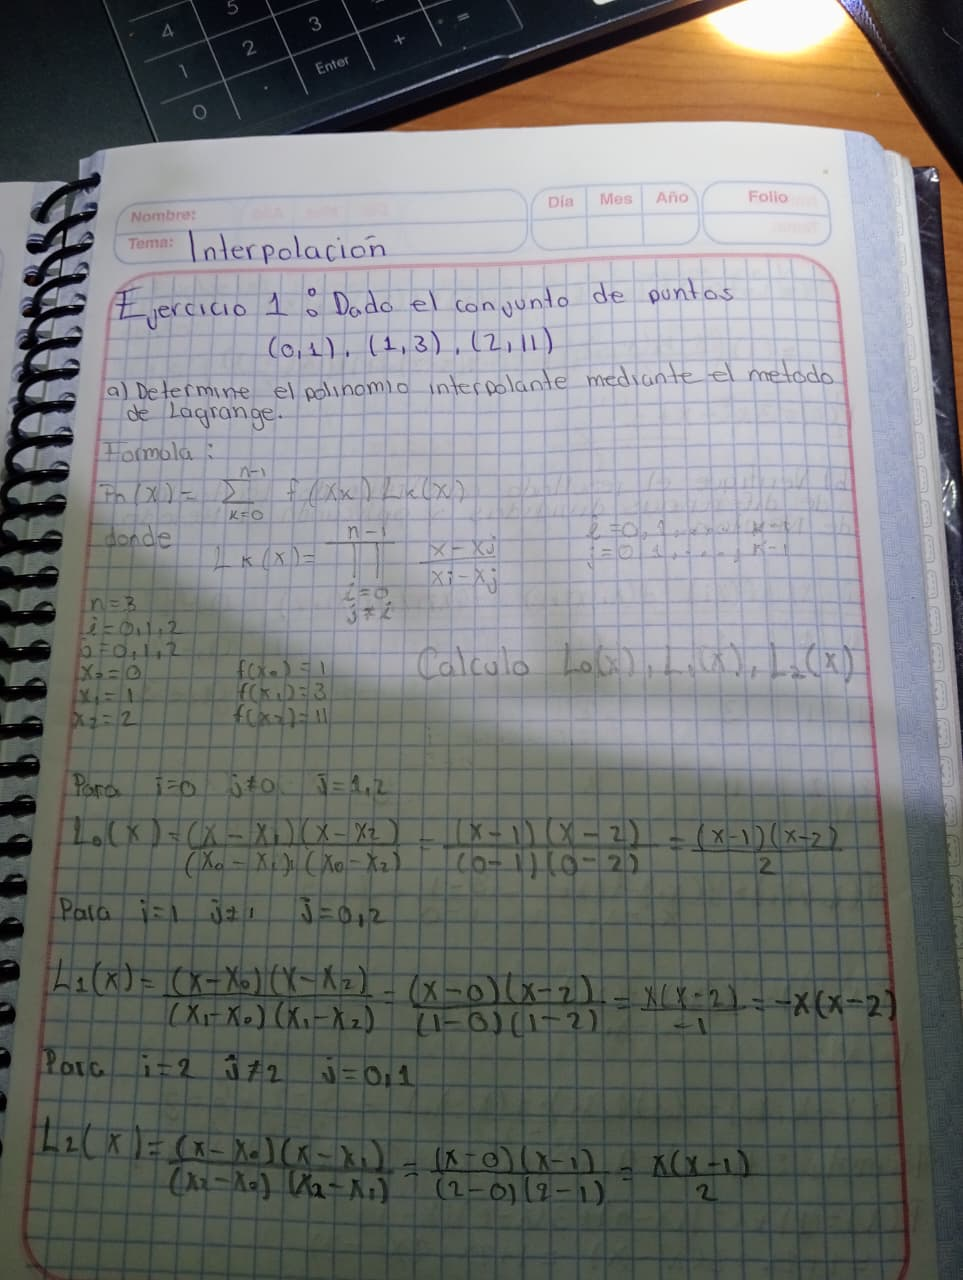
\includegraphics[width=2.60417in,height=\textheight,keepaspectratio,alt={pag.1}]{Interpolación_1.jpg}
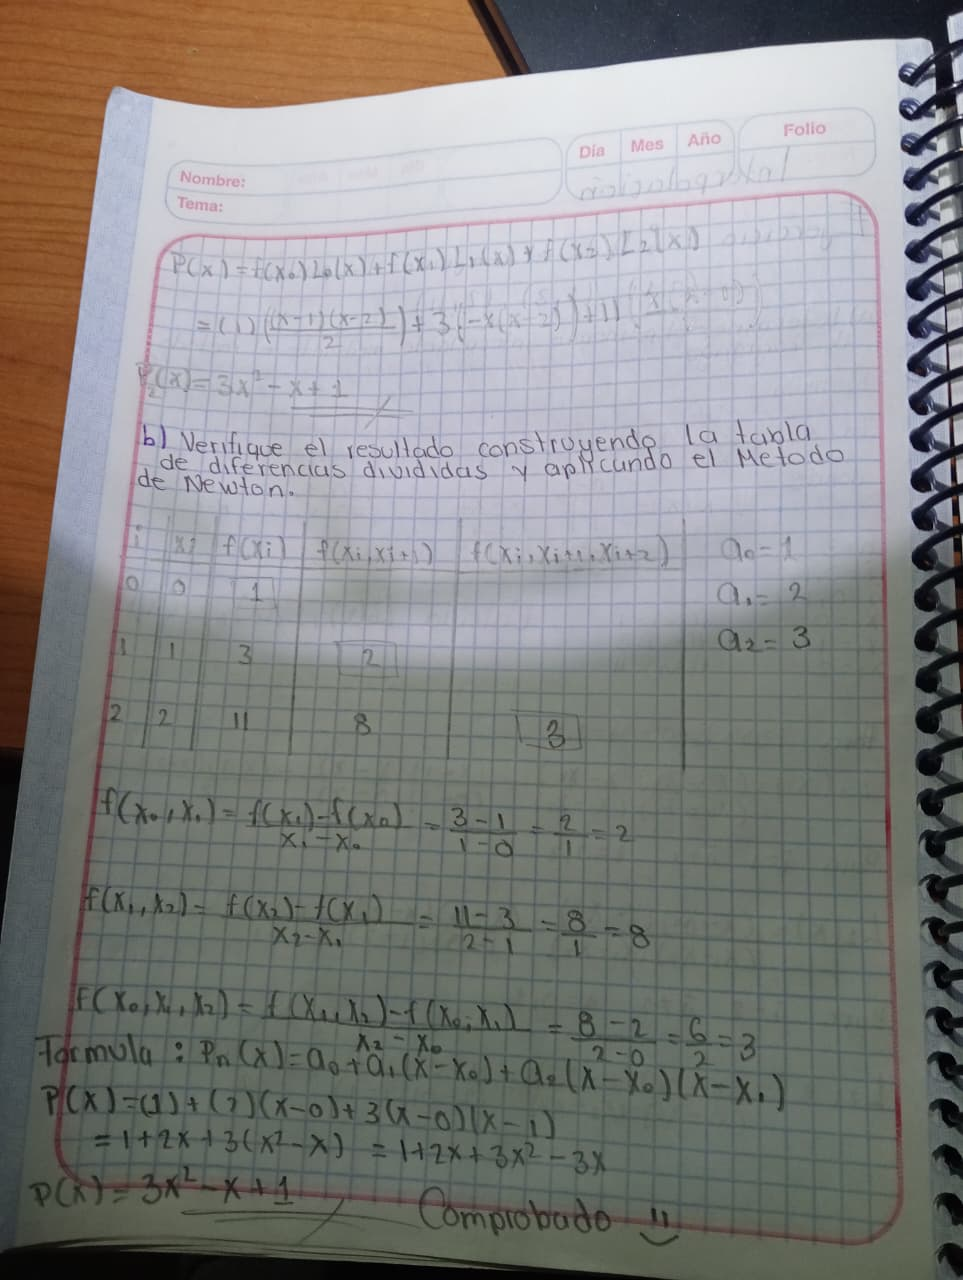
\includegraphics[width=2.60417in,height=\textheight,keepaspectratio,alt={pag.1}]{Interpolación_2.jpg}
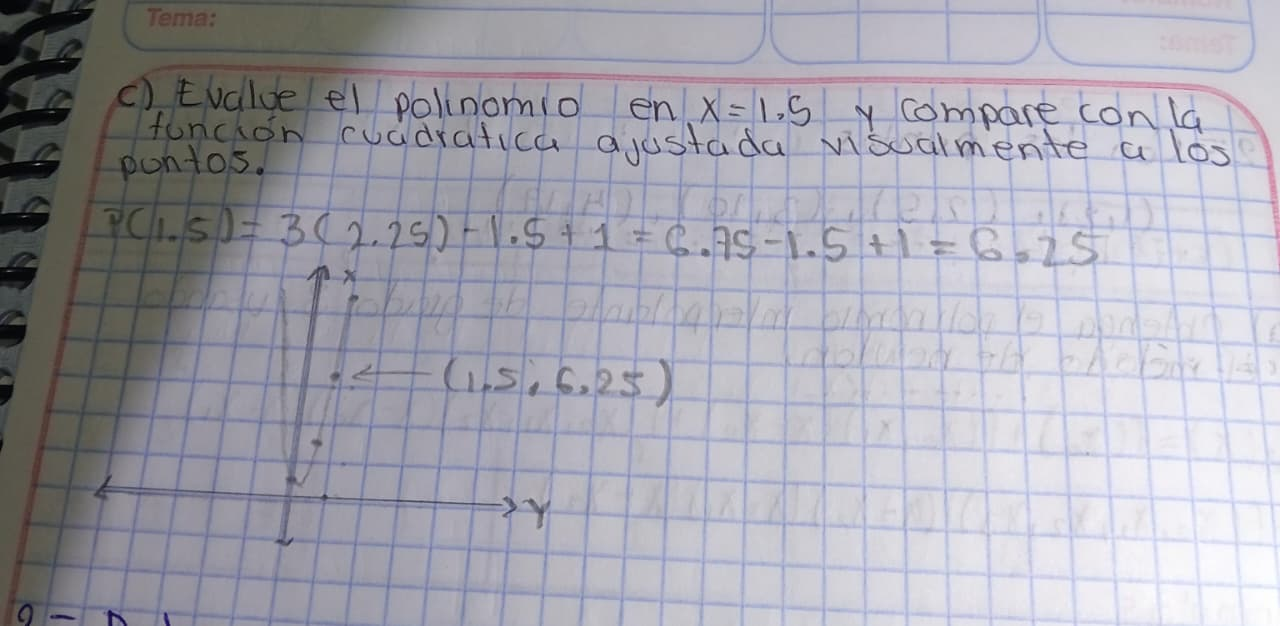
\includegraphics[width=2.60417in,height=\textheight,keepaspectratio,alt={pag.1}]{Interpolación_3.jpg}
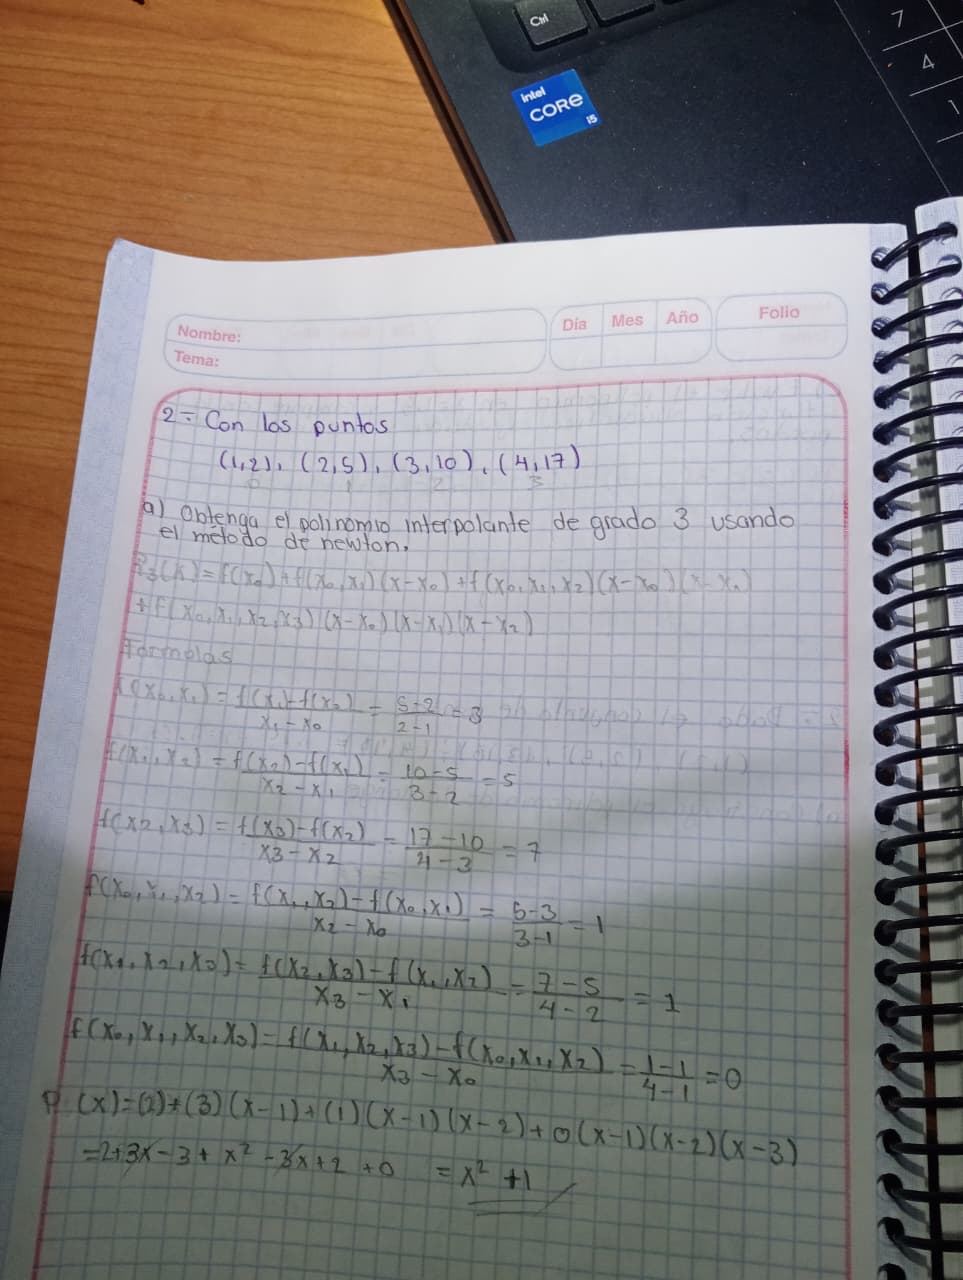
\includegraphics[width=2.60417in,height=\textheight,keepaspectratio,alt={pag.1}]{Interpolación_4.jpg}
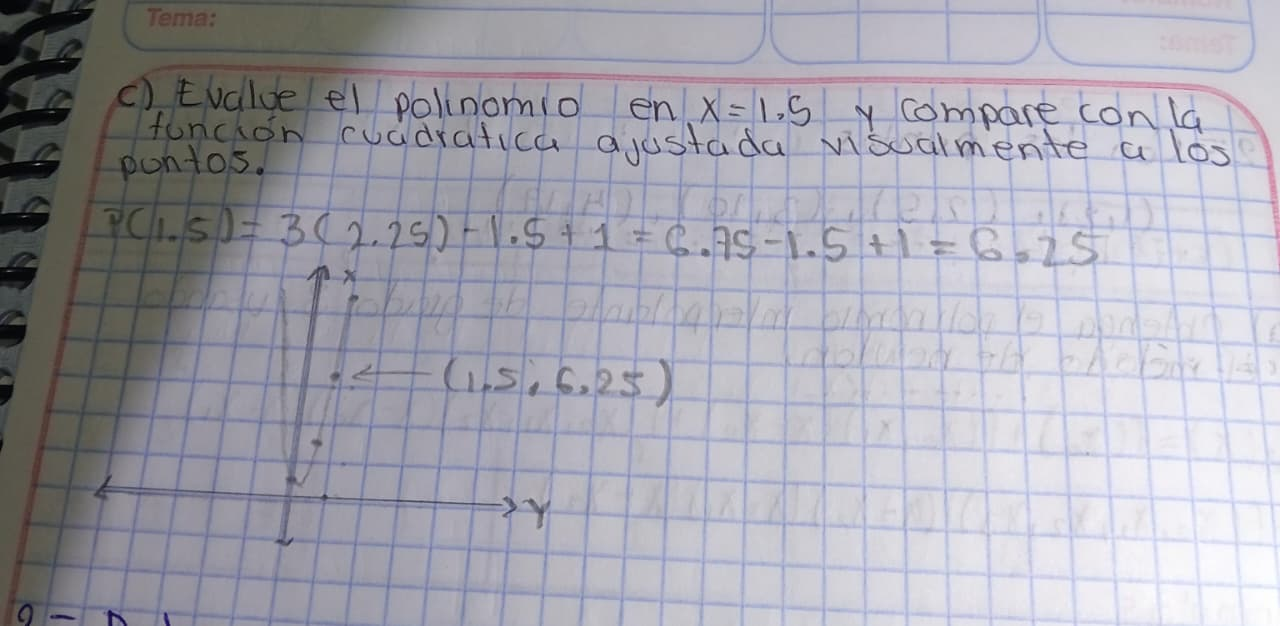
\includegraphics[width=2.60417in,height=\textheight,keepaspectratio,alt={pag.1}]{Interpolación_3.jpg}
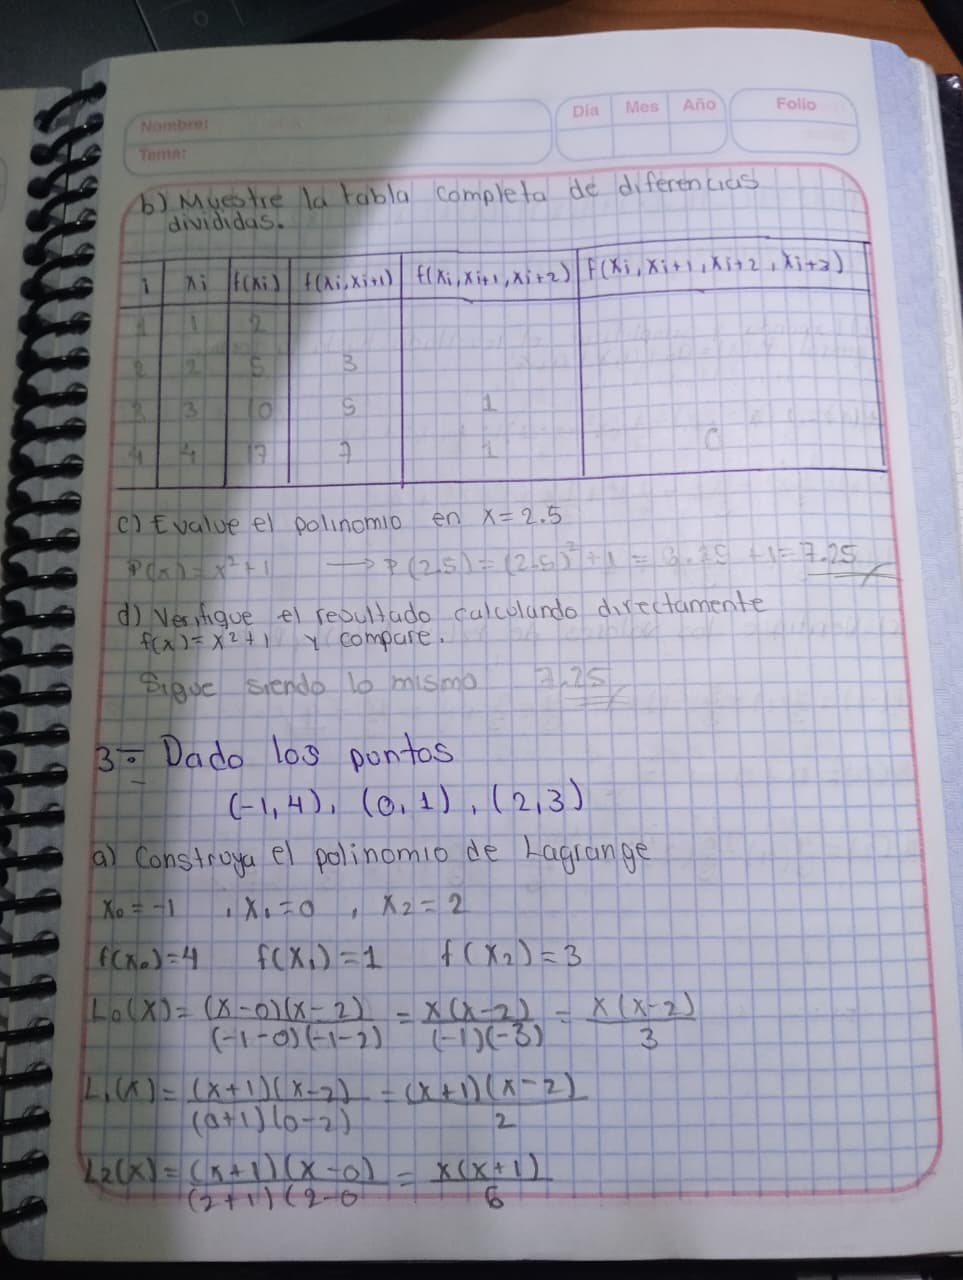
\includegraphics[width=2.60417in,height=\textheight,keepaspectratio,alt={pag.1}]{Interpolación_5.jpg}
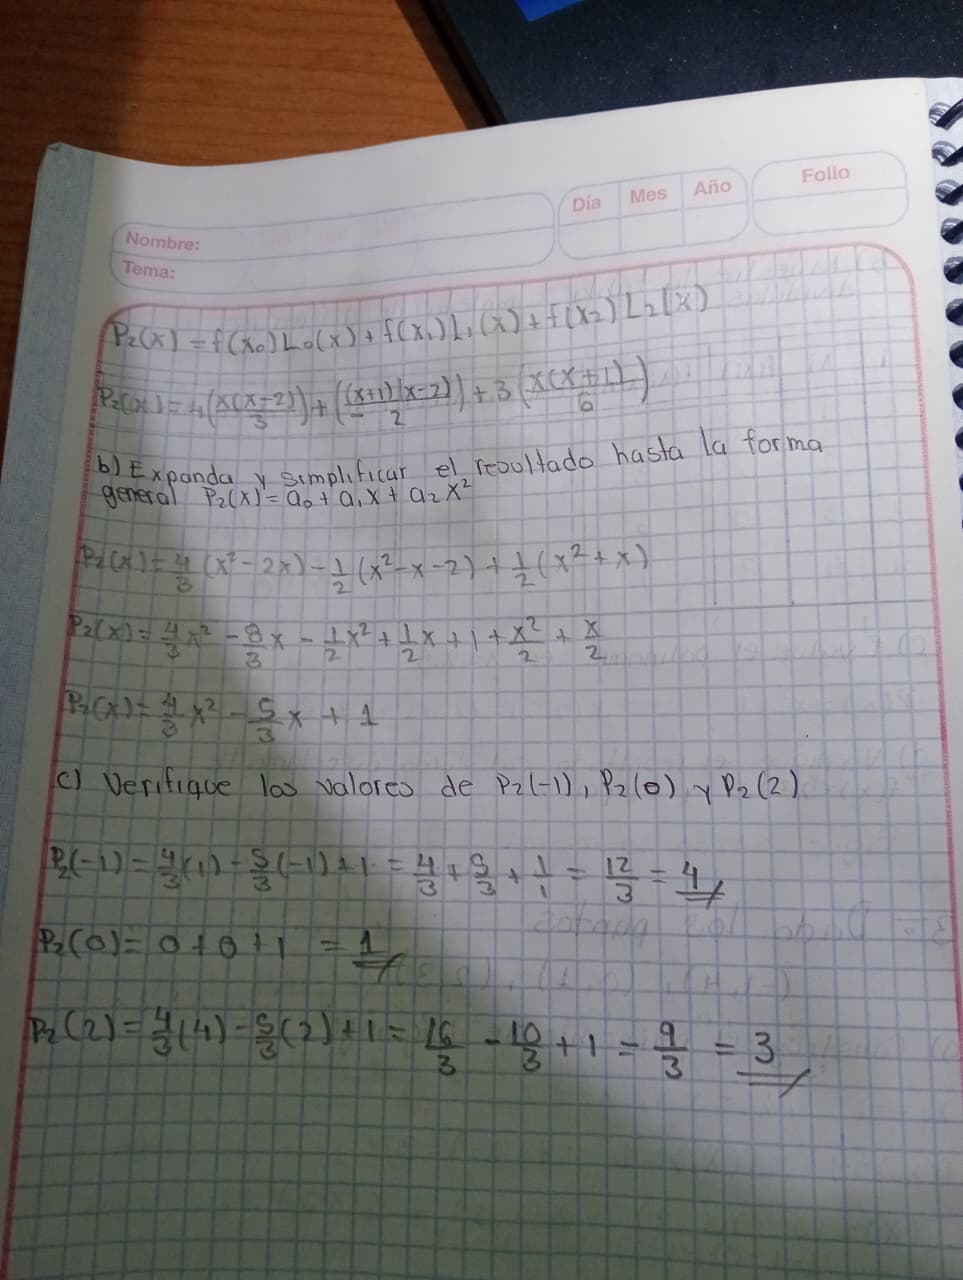
\includegraphics[width=2.60417in,height=\textheight,keepaspectratio,alt={pag.1}]{Interpolación_6.jpg}
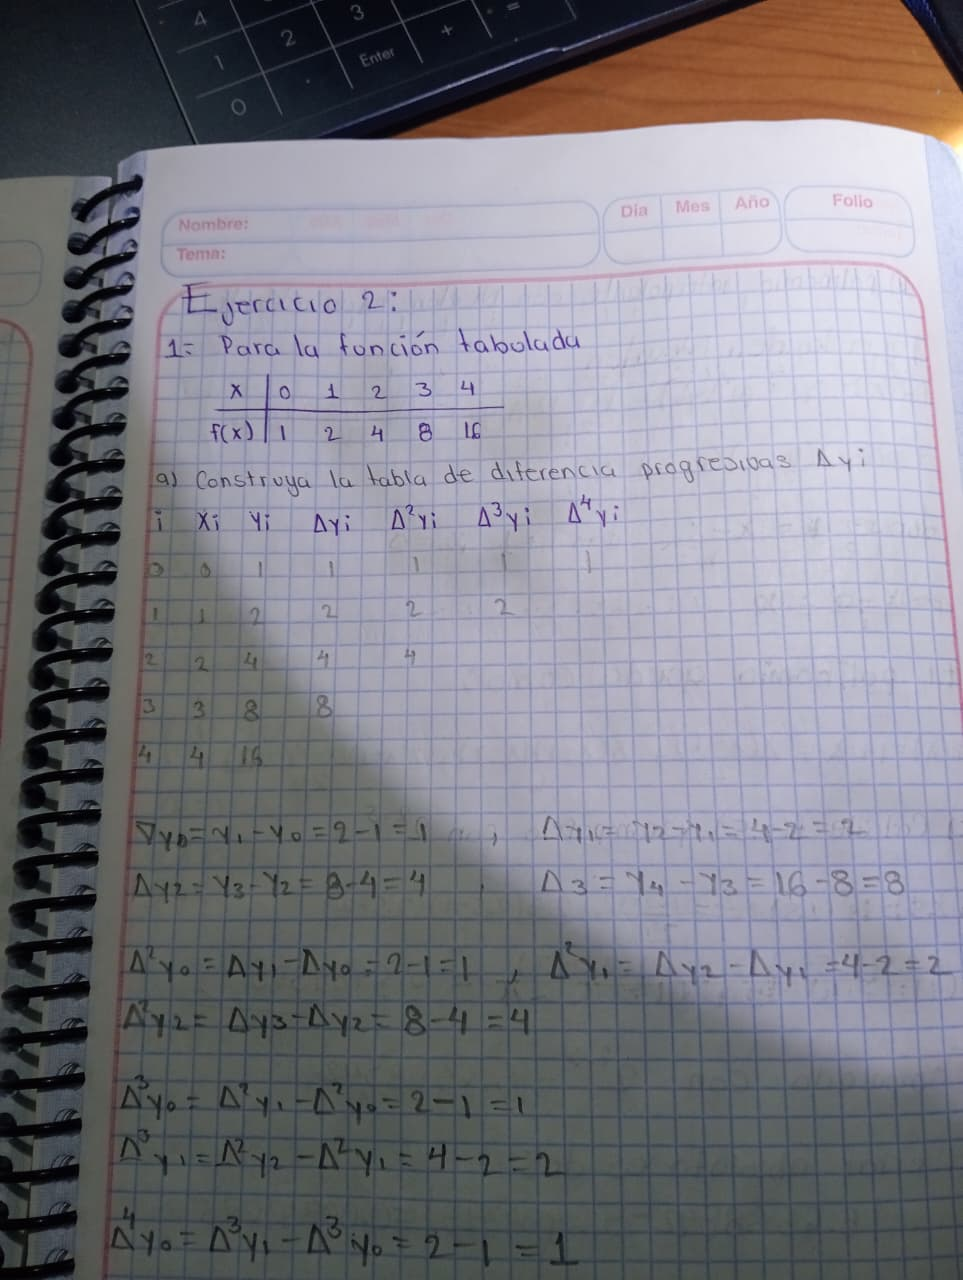
\includegraphics[width=2.60417in,height=\textheight,keepaspectratio,alt={pag.1}]{Interpolación_7.jpg}
\includegraphics[width=2.60417in,height=\textheight,keepaspectratio,alt={pag.1}]{\#\#\#**Verifcar que en la comprobación efectivamente se obtienen las igualdades** Interpolación_8.jpg}
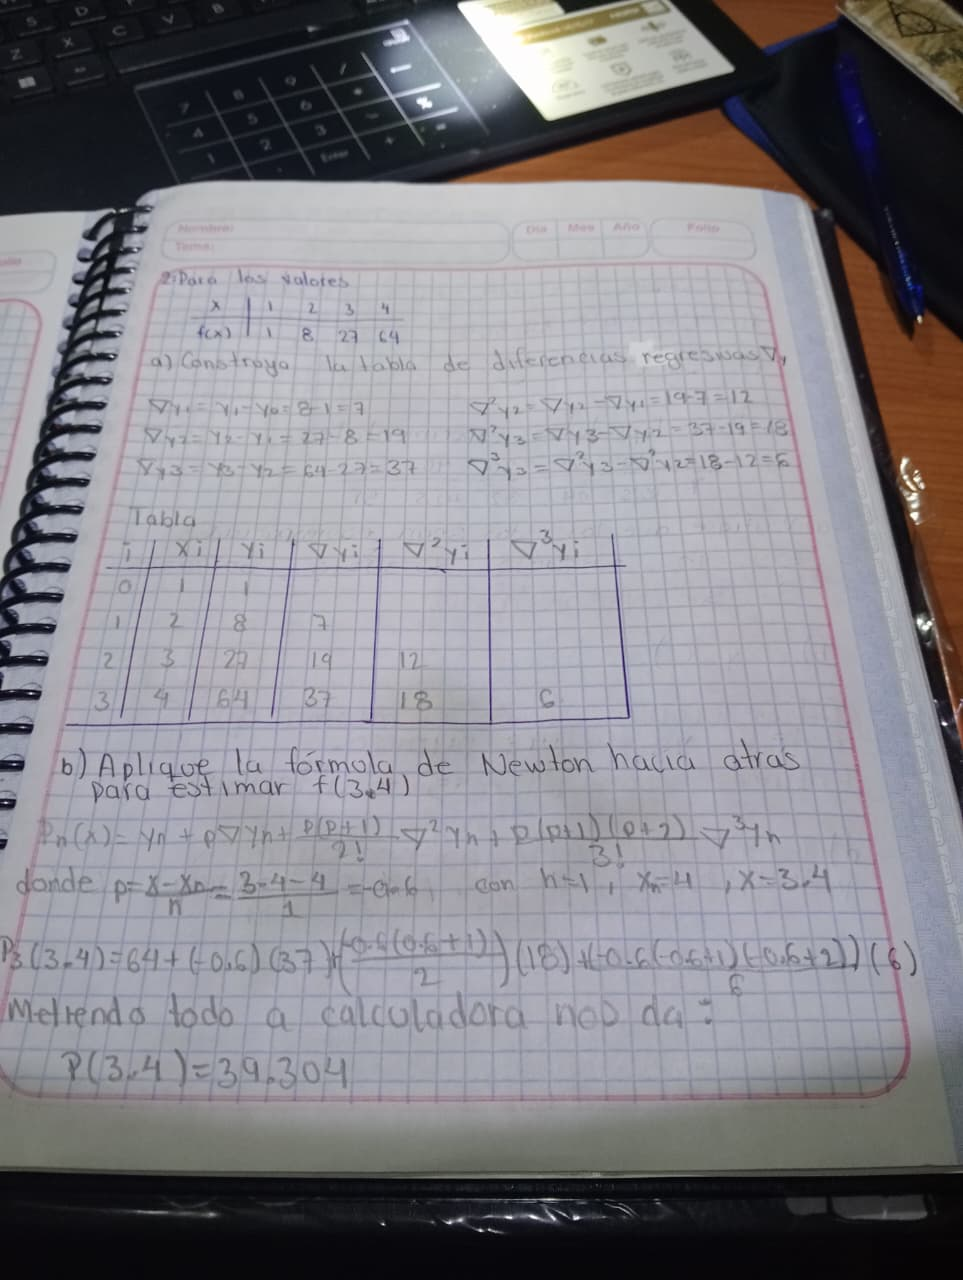
\includegraphics[width=2.60417in,height=\textheight,keepaspectratio,alt={pag.1}]{Interpolación_9.jpg}
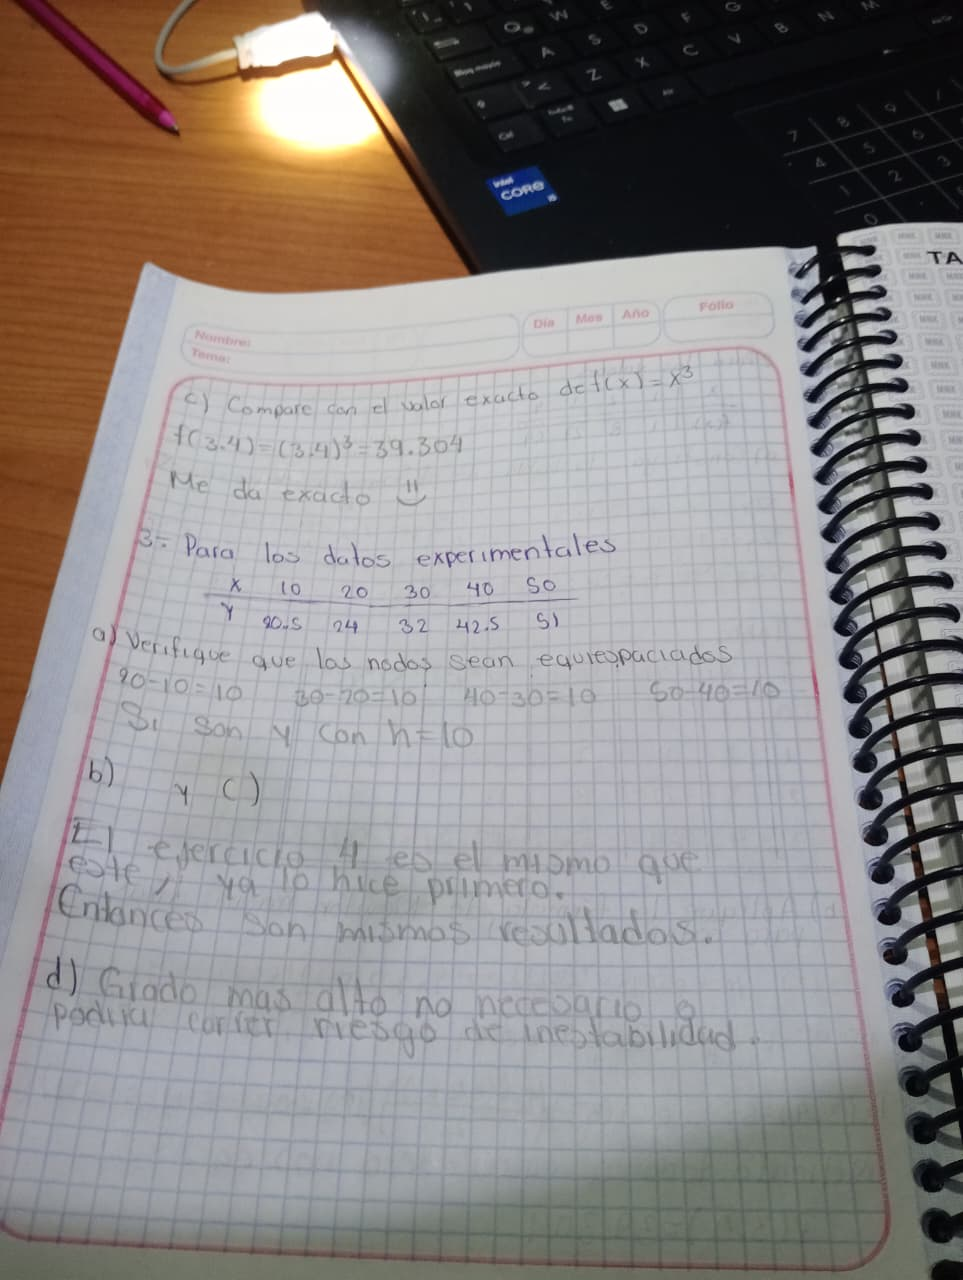
\includegraphics[width=2.60417in,height=\textheight,keepaspectratio,alt={pag.1}]{Interpolación_10.jpg}
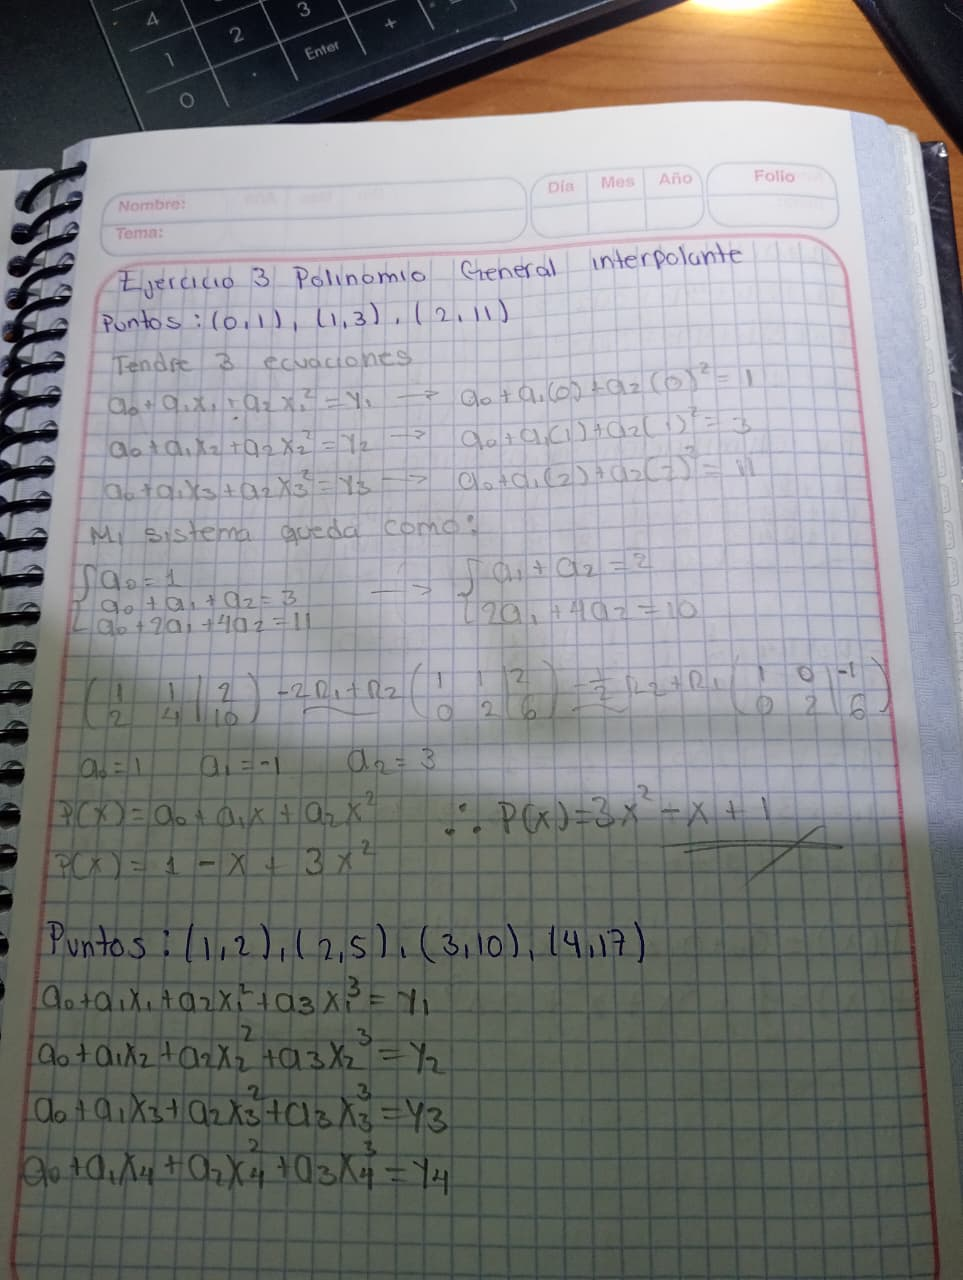
\includegraphics[width=2.60417in,height=\textheight,keepaspectratio,alt={pag.1}]{Interpolación_11.jpg}
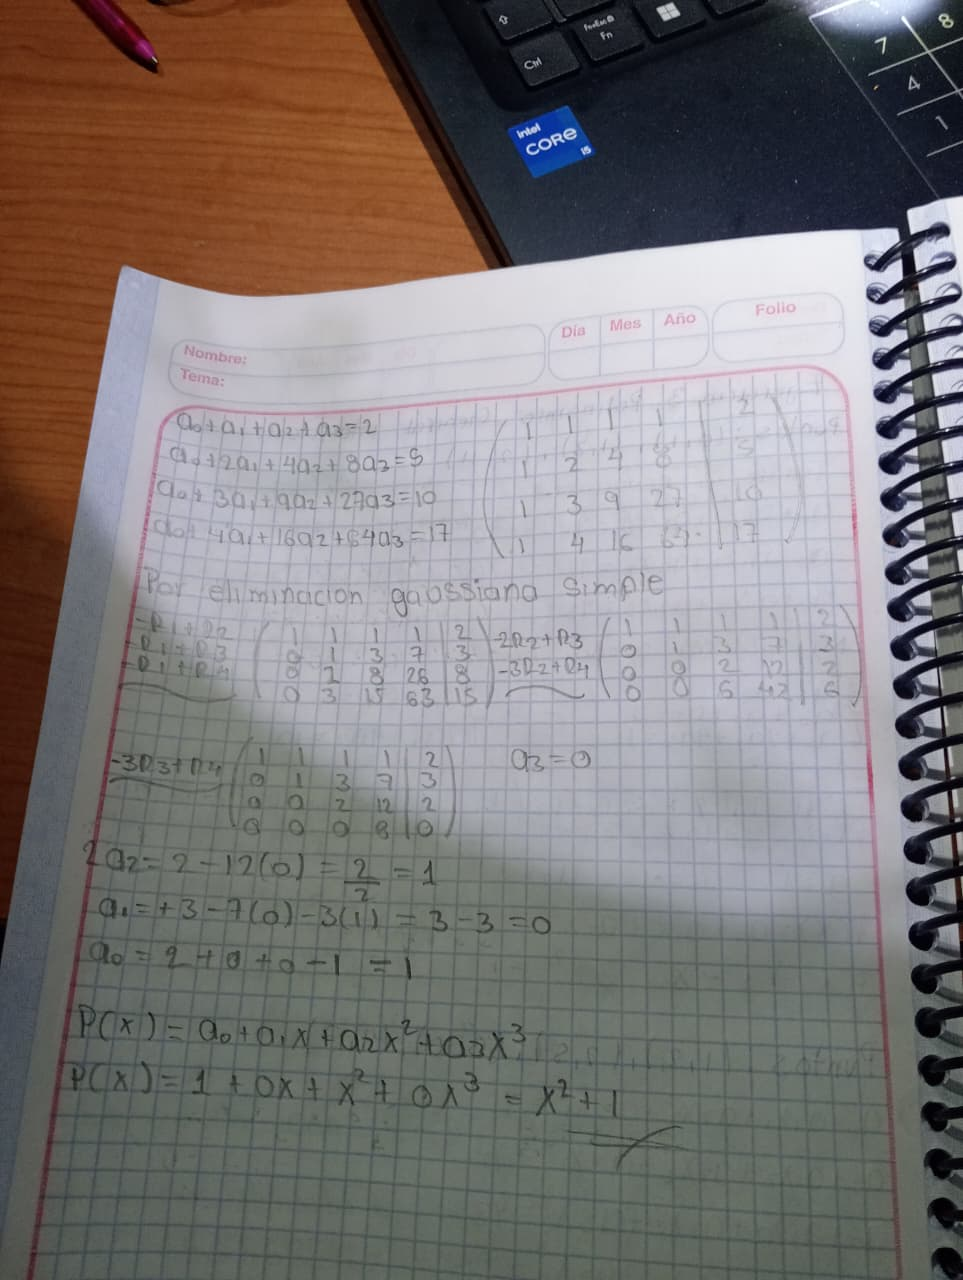
\includegraphics[width=2.60417in,height=\textheight,keepaspectratio,alt={pag.1}]{Interpolación_12.jpg}
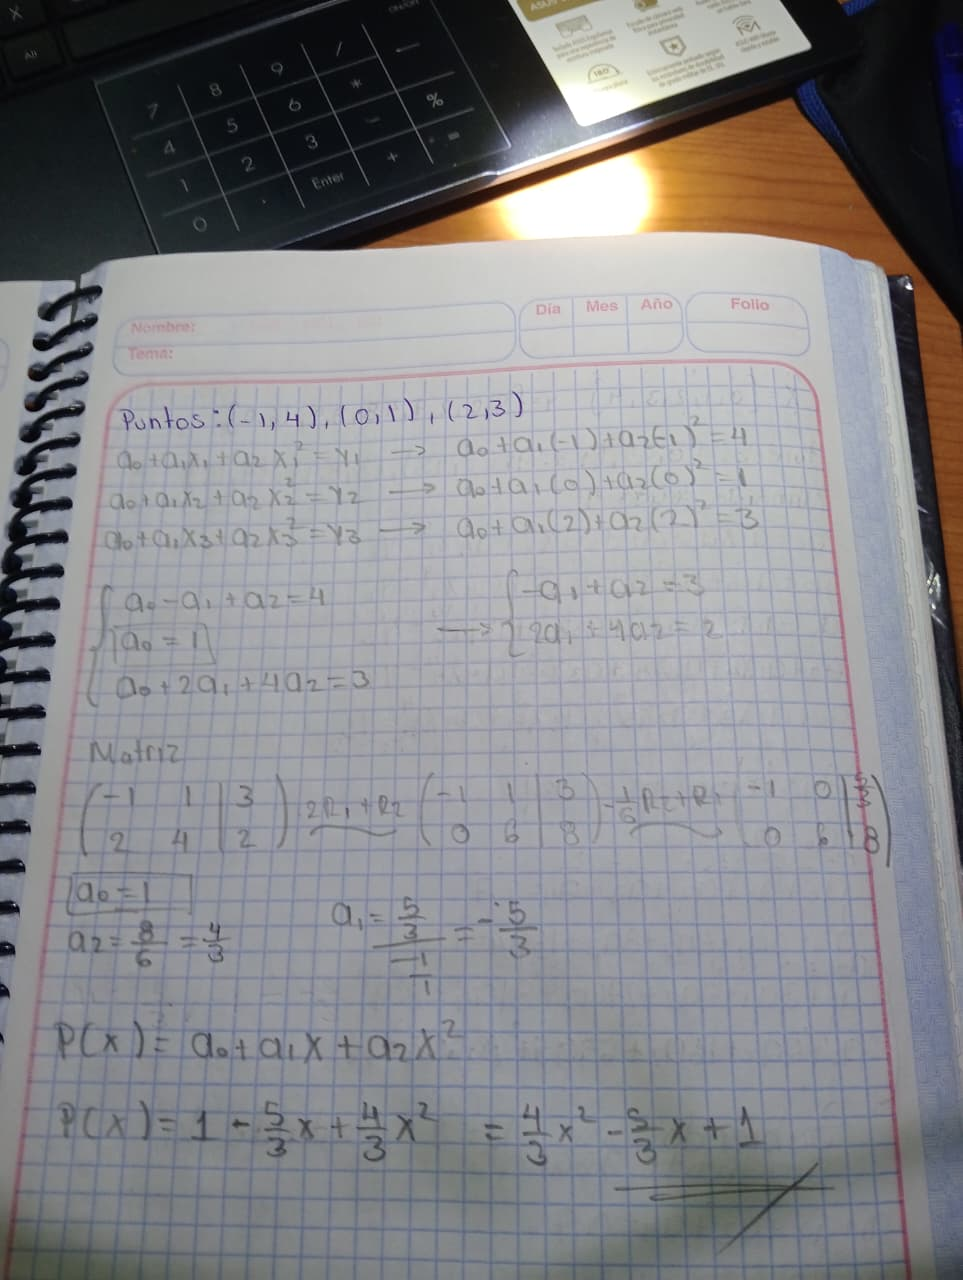
\includegraphics[width=2.60417in,height=\textheight,keepaspectratio,alt={pag.1}]{Interpolación_13.jpg}
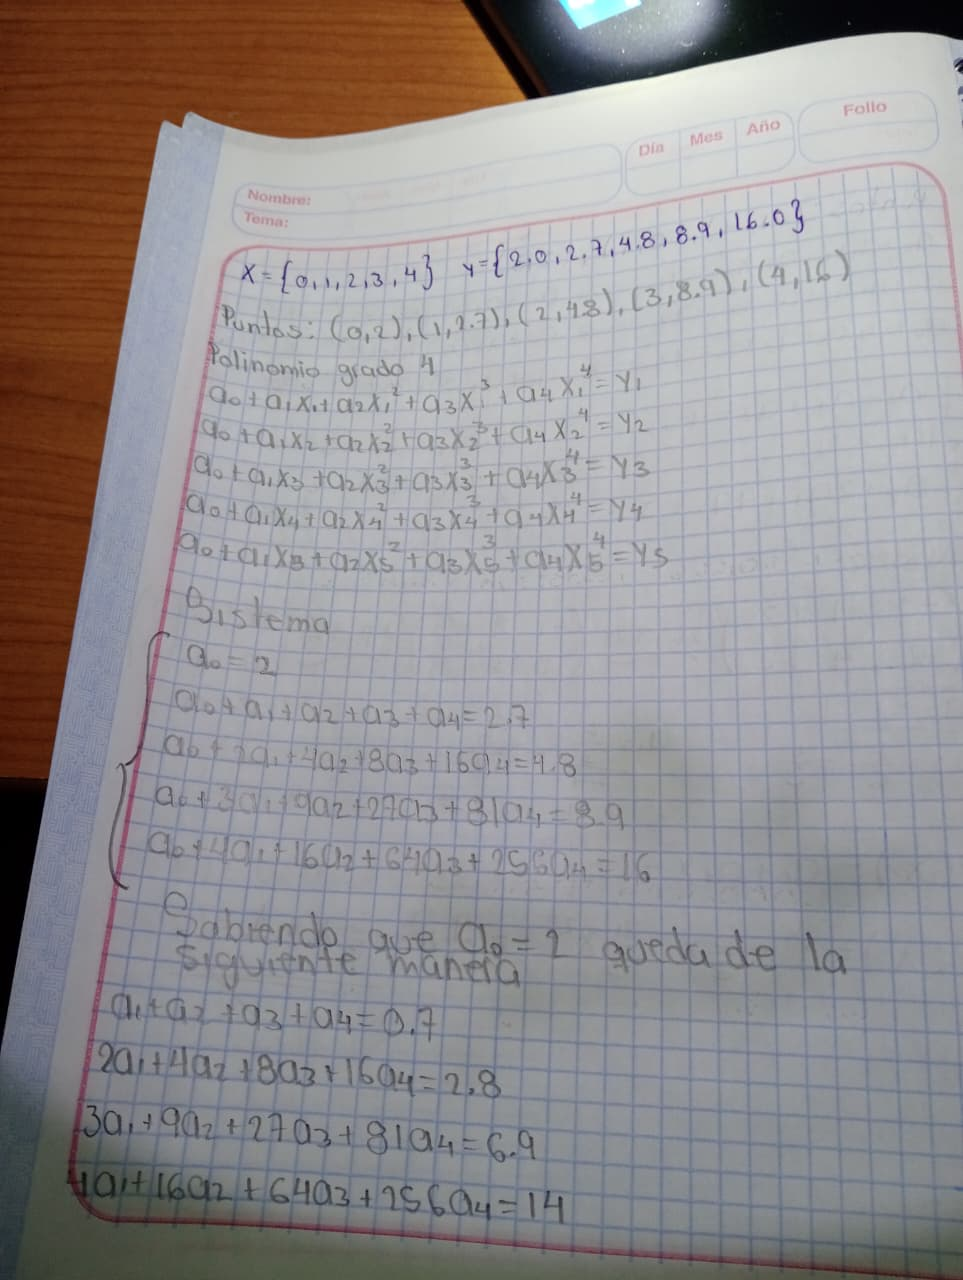
\includegraphics[width=2.60417in,height=\textheight,keepaspectratio,alt={pag.1}]{Interpolación_14.jpg}
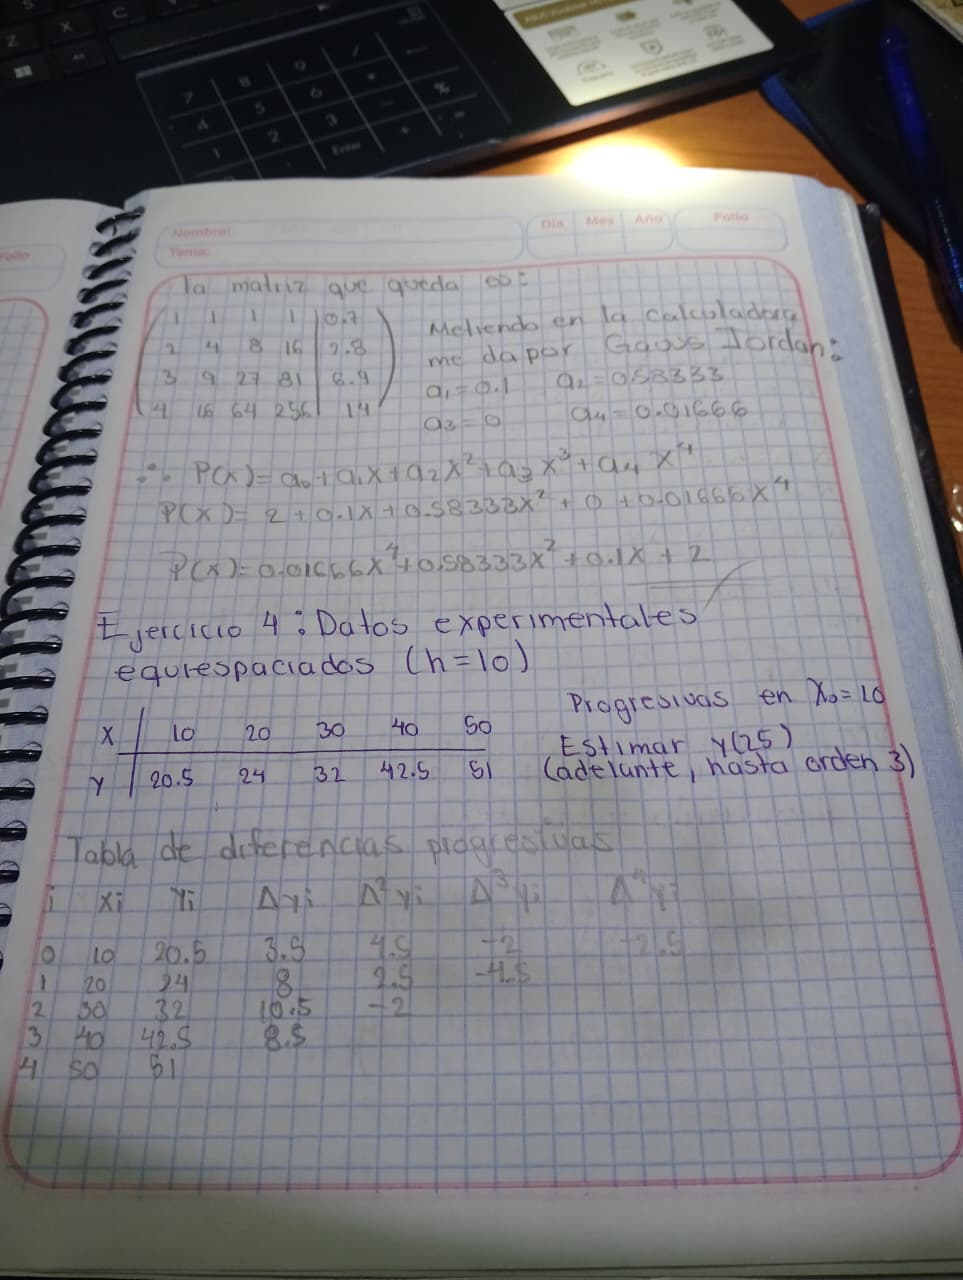
\includegraphics[width=2.60417in,height=\textheight,keepaspectratio,alt={pag.1}]{Interpolación_15.jpg}
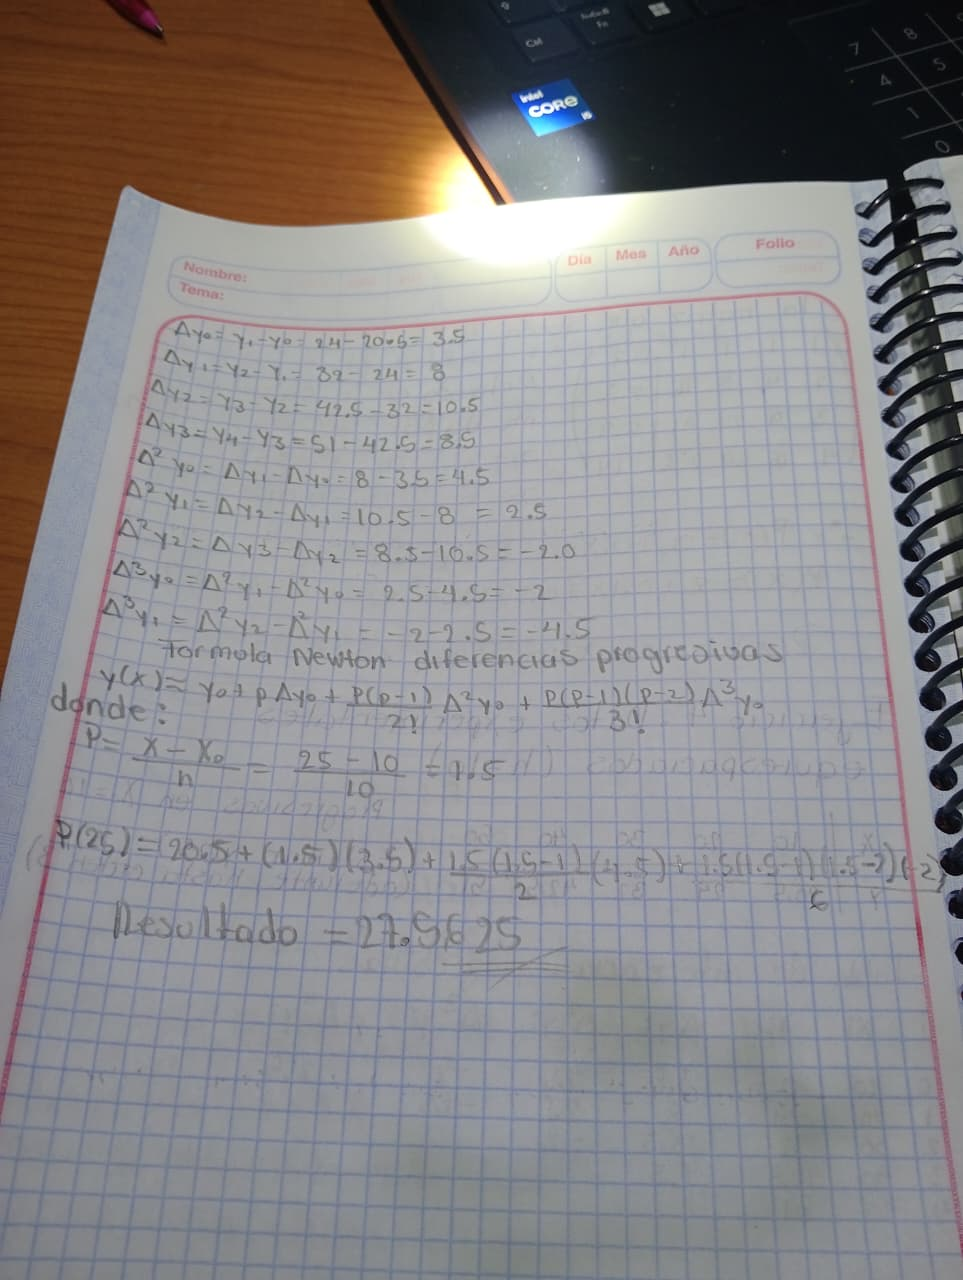
\includegraphics[width=2.60417in,height=\textheight,keepaspectratio,alt={pag.1}]{Interpolación_16.jpg}

\chapter{Observaciones}\label{observaciones}

\section{Sistemas de Ecuaciones
Lineales:}\label{sistemas-de-ecuaciones-lineales-1}

\begin{enumerate}
\def\labelenumi{\arabic{enumi})}
\item
  \emph{Verifcar que en la comprobación efectivamente se obtienen las
  igualdades}
\item
  \emph{Cuando se realicen las comprobaciones, realizarlas con valores
  redondeados, no los impresos}
\item
  \emph{Se vino un ``cat(''/)``, está de más, eliminar.}
\item
  \emph{En Gauss-Seidel aunque se menciona al inicio del ejercicio que
  no converge, hay que reafirmarlo al final.}
\item
  \emph{En Gauss-Seidel, con seis/siete ceros basta, 15-16 ya es
  prácticamete un cero-cero}
\item
  \emph{Valdría la pena graficas la soluciones en un plano para
  visualizar la estabilidad y estacionareidad de las soluciones}
\item
  \emph{Ver la posiblidad de manipular la gráfica para hacer una especie
  de zoom y líneas verticales que ayuden a interpretar mejor la gráfica}
\end{enumerate}

\backmatter
\end{document}
